% -----------------------------------------  
% Autogenerated LaTeX file from XML DocBook  
% -----------------------------------------  
%%<params>
%%</params>
\documentclass[letterpaper,10pt,twoside,openright]{book}
\IfFileExists{ifxetex.sty}{%
    \usepackage{ifxetex}%
  }{%
    \newif\ifxetex
    \xetexfalse
  }
  \ifxetex
\usepackage{fontspec}
\usepackage{xltxtra}
\setmainfont{DejaVu Serif}
\setsansfont{DejaVu Sans}
\setmonofont{DejaVu Sans Mono}
\else
\usepackage[T1]{fontenc}
\usepackage[latin1]{inputenc}
\fi
\usepackage{fancybox}
\usepackage{makeidx}
\usepackage[hyperlink]{cll}
\renewcommand{\DBKreleaseinfo}{}
\renewcommand{\DBKrevhistory}{}
\setcounter{tocdepth}{5}
\setcounter{secnumdepth}{5}
\def\DBKcopyright{\noindent Copyright \textnormal{\copyright} Test Copyright Year 2014 Test Copyright Holder}


\def\DBKsubtitle{Test Subtitle}



\title{The Complete Lojban Language}
\author{AuthorFirstName AuthorSurName}
\hypersetup{%
pdfcreator={DBLaTeX-0.3.4},%
pdftitle={The Complete Lojban Language},%
pdfauthor={AuthorFirstName AuthorSurName}%
}
\renewcommand{\DBKindexation}{}
\makeindex
\makeglossary
\begin{document}
\lstsetup
\frontmatter
\maketitle
\tableofcontents
\mainmatter

% ------- 
% Chapter 
% ------- 

\chapter{Lojban As We Mangle It In Lojbanistan: About This Book}
\label{chapter-about}\hyperlabel{chapter-about}%
    
\noindent\begin{minipage}[c]{\linewidth}
\begin{center}
\imgexists{media/chapter-about.gif}{{\imgevalsize{media/chapter-about.gif}{\includegraphics[width=\imgwidth,height=\imgheight,keepaspectratio=true]{media/chapter-about.gif}}}}{}\end{center}
\end{minipage}

   
\section{What is Lojban?}
\label{section-what-is-lojban}\hyperlabel{section-what-is-lojban}%
     
 \index{Logical Language Group!relation to Lojban} \index{Lojban!history of} Lojban (pronounced 
 “LOZH-{}bahn”) is a constructed language. Previous versions of the language were called 
 “Loglan” by Dr. James Cooke Brown, who founded the Loglan Project and started the development of the language in 1955. The goals for the language were first described in the open literature in the article 
   “\emph{Loglan}”, published in 
 \emph{Scientific American}, June, 1960. Made well-{}known by that article and by occasional references in science fiction (most notably in Robert Heinlein's novel 
  \emph{The Moon Is A Harsh Mistress}) and computer publications, Loglan and Lojban have been built over four decades by dozens of workers and hundreds of supporters, led since 1987 by The Logical Language Group (who are the publishers of this book).
  
 \index{Lojban!features of} There are thousands of artificial languages (of which Esperanto is the best-{}known), but Loglan/Lojban has been engineered to make it unique in several ways. The following are the main features of Lojban:
  \begin{itemize}

\item{}  Lojban is designed to be used by people in communication with each other, and possibly in the future with computers.
  

\item{}  Lojban is designed to be neutral between cultures.
  

\item{}  Lojban grammar is based on the principles of predicate logic.
  

\item{}  Lojban has an unambiguous yet flexible grammar.
  

\item{}  Lojban has phonetic spelling, and unambiguously resolves its sounds into words.
  

\item{}  Lojban is simple compared to natural languages; it is easy to learn.
  

\item{}  Lojban's 1300 root words can be easily combined to form a vocabulary of millions of words.
  

\item{}  Lojban is regular; the rules of the language are without exceptions.
  

\item{}  Lojban attempts to remove restrictions on creative and clear thought and communication.
  

\item{}  Lojban has a variety of uses, ranging from the creative to the scientific, from the theoretical to the practical.
  

\item{}  Lojban has been demonstrated in translation and in original works of prose and poetry.
  
\end{itemize}
    
\section{What is this book?}
\label{section-what-is-cll}\hyperlabel{section-what-is-cll}%
    
 \index{goal of this book} \index{this book!goal of} \index{reference grammar} This book is what is called a 
 “reference grammar”. It attempts to expound the whole Lojban language, or at least as much of it as is understood at present. Lojban is a rich language with many features, and an attempt has been made to discover the functions of those features. The word 
  “discover” is used advisedly; Lojban was not 
 “invented” by any one person or committee. Often, grammatical features were introduced into the language long before their usage was fully understood. Sometimes they were introduced for one reason, only to prove more useful for other reasons not recognized at the time.
  
By intention, this book is complete in description but not in explanation. For every rule in the formal Lojban grammar (given in 
 Chapter \ref{chapter-grammars}), there is a bit of explanation and an example somewhere in the book, and often a great deal more than a bit. In essence, 
 Chapter \ref{chapter-tour} gives a brief overview of the language, 
 Chapter \ref{chapter-grammars} gives the formal structure of the language, and the chapters in between put semantic flesh on those formal bones. I hope that eventually more grammatical material founded on (or even correcting) the explanations in this book will become available.
  
 \index{linguistic drift} \index{Lojban!stability of} Nevertheless, the publication of this book is, in one sense, the completion of a long period of language evolution. With the exception of a possible revision of the language that will not even be considered until five years from publication date, and any revisions of this book needed to correct outright errors, the language described in this book will not be changing by deliberate act of its creators any more. Instead, language change will take place in the form of new vocabulary – Lojban does not yet have nearly the vocabulary it needs to be a fully usable language of the modern world, as 
 Chapter \ref{chapter-lujvo} explains – and through the irregular natural processes of drift and (who knows?) native-{}speaker evolution. (Teach your children Lojban!) You can learn the language described here with assurance that (unlike previous versions of Lojban and Loglan, as well as most other artificial languages) it will not be subject to further fiddling by language-{}meisters.
  
 \index{this book!structure of} \index{structure of this book} It is probably worth mentioning that this book was written somewhat piecemeal. Each chapter began life as an explication of a specific Lojban topic; only later did these begin to clump together into a larger structure of words and ideas. Therefore, there are perhaps not as many cross-{}references as there should be. However, I have attempted to make the index as comprehensive as possible.
  
 \index{chapter titles!intent of} \index{jokes} \index{Lojbanistan} Each chapter has a descriptive title, often involving some play on words; this is an attempt to make the chapters more memorable. The title of 
 Chapter \ref{chapter-about} (which you are now reading), for example, is an allusion to the book 
 \emph{English As We Speak It In Ireland}, by P. W. Joyce, which is a sort of informal reference grammar of Hiberno-{}English. 
  “Lojbanistan” is both an imaginary country where Lojban is the native language, and a term for the actual community of Lojban-{}speakers, scattered over the world. Why 
  “mangle”? As yet, nobody in the real Lojbanistan speaks the language at all well, by the standards of the imaginary Lojbanistan; that is one of the circumstances this book is meant to help remedy.
     
\section{What are the typographical conventions of this book?}
\label{section-conventions}\hyperlabel{section-conventions}%
     
Each chapter is broken into numbered sections; each section contains a mixture of expository text, numbered examples, and possibly tables.
  
 \index{this book!examples of} \index{examples in this book} The reader will notice a certain similarity in the examples used throughout the book. One chapter after another rings the changes on the self-{}same sentences:
  
\begin{longfloat}{example}{\caption[{   }]{   \index{go to the store!example}    \label{c1e3d1}\hyperlabel{c1e3d1}  }
\label{example-random-id-hrtj}\hyperlabel{example-random-id-hrtj}%
}

\begin{tabulary}{\linewidth}{LLLL}
{}mi&
{}klama&
{}le&
{}zarci\tabularnewline
{}I&
{}go-{}to&
{}that-{}which-{}I-{}describe-{}as-{}a&
{}store.\tabularnewline
\multicolumn{4}{l}{
I go to the store.
}\tabularnewline
\end{tabulary}

\end{longfloat}
  
  will become wearisomely familiar before 
 Chapter \ref{chapter-grammars} is reached. This method is deliberate; I have tried to use simple and (eventually) familiar examples wherever possible, to avoid obscuring new grammatical points with new vocabulary. Of course, this is not the method of a textbook, but this book is not a textbook (although people have learned Lojban from it and its predecessors). Rather, it is intended both for self-{}learning (of course, at present would-{}be Lojban teachers must be self-{}learners) and to serve as a reference in the usual sense, for looking up obscure points about the language.
  
 \index{examples!structure of} \index{structure of examples} \index{example of examples} It is useful to talk further about 
 Example \ref{example-random-id-hrtj} for what it illustrates about examples in this book. Examples usually occupy three lines. The first of these is in Lojban, the second in a word-{}by-{}word literal translation of the Lojban into English, and the third in colloquial English. The second and third lines are sometimes called the 
  “literal translation” and the 
 “colloquial translation” respectively. Sometimes, when clarity is not sacrificed thereby, one or both are omitted. If there is more than one Lojban sentence, it generally means that they have the same meaning.
  
 \index{square brackets!use of in notation} Words are sometimes surrounded by square brackets. In Lojban texts, these enclose optional grammatical particles that may (in the context of the particular example) be either omitted or included. In literal translations, they enclose words that are used as conventional translations of specific Lojban words, but don't have exactly the meanings or uses that the English word would suggest. In 
  Chapter \ref{chapter-phonology}, square brackets surround phonetic representations in the International Phonetic Alphabet.
   
 \index{grammatical categories!use of upper case for} \index{tables!format of} Many of the tables, especially those placed at the head of various sections, are in three columns. The first column contains Lojban words discussed in that section; the second column contains the grammatical category (represented by an UPPER CASE Lojban word) to which the word belongs, and the third column contains a brief English gloss, not necessarily or typically a full explanation. Other tables are explained in context.
  
 \index{technical terms} A few Lojban words are used in this book as technical terms. All of these are explained in 
  Chapter \ref{chapter-tour}, except for a few used only in single chapters, which are explained in the introductory sections of those chapters.
    
\section{Disclaimers}
\label{section-disclaimers}\hyperlabel{section-disclaimers}%
    
 \index{disclaimers} It is necessary to add, alas, that the examples used in this book do not refer to any existing person, place, or institution, and that any such resemblance is entirely coincidental and unintentional, and not intended to give offense.
  
 \index{dictionary!superior authority of} When definitions and place structures of gismu, and especially of lujvo, are given in this book, they may differ from those given in the English-{}Lojban dictionary (which, as of this writing, is not yet published). If so, the information given in the dictionary supersedes whatever is given here.
    
\section{Acknowledgements and Credits}
\label{credits}\hyperlabel{credits}%
    
 \index{LLG} \index{this book!author of} \index{author of this book} Although the bulk of this book was written for the Logical Language Group (LLG) by John Cowan, who is represented by the occasional authorial 
  “I”, certain chapters were first written by others and then heavily edited by me to fit into this book.
  
 \index{this book!contributors to} \index{contributors to this book} In particular: 
 Chapter \ref{chapter-tour} is a fusion of originally separate documents, one by Athelstan, and one by Nora Tansky LeChevalier and Bob LeChevalier; 
 Chapter \ref{chapter-phonology} and 
 Chapter \ref{chapter-morphology} were originally written by Bob LeChevalier with contributions by Chuck Barton; 
 Chapter \ref{chapter-lujvo} was originally written (in much longer form) by Nick Nicholas; the dialogue near the end of 
 Chapter \ref{chapter-attitudinals} was contributed by Nora Tansky LeChevalier; 
 Chapter \ref{chapter-negation} and parts of 
 Chapter \ref{chapter-quantifiers} were originally by Bob LeChevalier; and the YACC grammar in 
  Chapter \ref{chapter-grammars} is the work of several hands, but is primarily by Bob LeChevalier and Jeff Taylor. The BNF grammar, which is also in 
 Chapter \ref{chapter-grammars}, was originally written by me, then rewritten by Clark Nelson, and finally touched up by me again.
  
 \index{this book!credits for} \index{credits for this book} The research into natural languages from which parts of 
 Chapter \ref{chapter-selbri} draw their material was performed by Ivan Derzhanski. LLG acknowledges his kind permission to use the fruits of his research.
   
 \index{pictures!credits for} \index{credits for pictures} The pictures in this book were drawn by Nora Tansky LeChevalier, except for the picture appearing in 
  Chapter \ref{chapter-morphology}, which is by Sylvia Rutiser Rissell.
  
The index was made by Nora Tansky LeChevalier.
  
 \index{this book!reviewers of} \index{reviewers of this book} I would like to thank the following people for their detailed reviews, suggestions, comments, and early detection of my embarrassing errors in Lojban, logic, English, and cross-{}references: Nick Nicholas, Mark Shoulson, Veijo Vilva, Colin Fine, And Rosta, Jorge Llambias, Iain Alexander, Paulo S. L. M. Barreto, Robert J. Chassell, Gale Cowan, Karen Stein, Ivan Derzhanski, Jim Carter, Irene Gates, Bob LeChevalier, John Parks-{}Clifford (also known as 
 “pc”), and Nora Tansky LeChevalier.
  
Nick Nicholas (NSN) would like to thank the following Lojbanists: Mark Shoulson, Veijo Vilva, Colin Fine, And Rosta, and Iain Alexander for their suggestions and comments; John Cowan, for his extensive comments, his exemplary trailblazing of Lojban grammar, and for solving the 
 \hyperlink{valsi-manskapi}{\emph{\emph{\index{manskapi}manskapi}}} dilemma for NSN; Jorge Llambias, for his even more extensive comments, and for forcing NSN to think more than he was inclined to; Bob LeChevalier, for his skeptical overview of the issue, his encouragement, and for scouring all Lojban text his computer has been burdened with for lujvo; Nora Tansky LeChevalier, for writing the program converting old rafsi text to new rafsi text, and sparing NSN from embarrassing errors; and Jim Carter, for his dogged persistence in analyzing lujvo algorithmically, which inspired this research, and for first identifying the three lujvo classes.
   
 \index{Brown!James Cooke} Of course, the entire Loglan Project owes a considerable debt to James Cooke Brown as the language inventor, and also to several earlier contributors to the development of the language. Especially noteworthy are Doug Landauer, Jeff Prothero, Scott Layson, Jeff Taylor, and Bob McIvor. Final responsibility for the remaining errors and infelicities is solely mine.
     
\section{Informal Bibliography}
\label{section-bibliography}\hyperlabel{section-bibliography}%
    
 \index{Loglan} \index{bibliography} The founding document for the Loglan Project, of which this book is one of the products, is 
 \emph{Loglan 1: A Logical Language} by James Cooke Brown (4th ed. 1989, The Loglan Institute, Gainesville, Florida, U.S.A.). The language described therein is not Lojban, but is very close to it and may be considered an ancestral version. It is regrettably necessary to state that nothing in this book has been approved by Dr. Brown, and that the very existence of Lojban is disapproved of by him.
   
The logic of Lojban, such as it is, owes a good deal to the American philosopher W. v.O. Quine, especially 
 \emph{Word and Object} (1960, M.I.T. Press). Much of Quine's philosophical writings, especially on observation sentences, reads like a literal translation from Lojban.
   
The theory of negation expounded in 
 Chapter \ref{chapter-negation} is derived from a reading of Laurence Horn's work 
 \emph{A Natural History of Negation}.
  
Of course, neither Brown nor Quine nor Horn is in any way responsible for the uses or misuses I have made of their works.
   
 \index{books about Lojban} Depending on just when you are reading this book, there may be three other books about Lojban available: a textbook, a Lojban/English dictionary, and a book containing general information about Lojban. You can probably get these books, if they have been published, from the same place where you got this book. In addition, other books not yet foreseen may also exist.
     
\section{Captions to Pictures}
\label{section-captions}\hyperlabel{section-captions}%
    
The following examples list the Lojban caption, with a translation, for the picture at the head of each chapter. If a chapter's picture has no caption, 
 “(none)” is specified instead.
  
\subsection[{Chapter 1 Caption}]{\hyperlink{chapter-about-picture}{Chapter 1 Caption}}
    
\begin{lstlisting}[firstnumber=1,]
        coi lojban.             coi rodo
      \end{lstlisting}
  
\begin{lstlisting}[firstnumber=1,]
        Greetings, O Lojban!    Greetings, all-of you
      \end{lstlisting}
    
\subsection[{Chapter 2 Caption}]{\hyperlink{chapter-tour-picture}{Chapter 2 Caption}}
    
\begin{lstlisting}[firstnumber=1,]
        (none)
      \end{lstlisting}
    
\subsection[{Chapter 3 Caption}]{\hyperlink{chapter-phonology-picture}{Chapter 3 Caption}}
    
\begin{lstlisting}[firstnumber=1,]
        .i .ai .i .ai .o
      \end{lstlisting}
  
\begin{lstlisting}[firstnumber=1,]
        [untranslatable]
      \end{lstlisting}
    
\subsection[{Chapter 4 Caption}]{\hyperlink{chapter-morphology-picture}{Chapter 4 Caption}}
    
\begin{lstlisting}[firstnumber=1,]
        jbobliku
      \end{lstlisting}
  
\begin{lstlisting}[firstnumber=1,]
        Lojbanic-blocks
      \end{lstlisting}
    
\subsection[{Chapter 5 Caption}]{\hyperlink{chapter-selbri-picture}{Chapter 5 Caption}}
    
\begin{lstlisting}[firstnumber=1,]
        (none)
      \end{lstlisting}
    
\subsection[{Chapter 6 Caption}]{\hyperlink{chapter-sumti-picture}{Chapter 6 Caption}}
    
\begin{lstlisting}[firstnumber=1,]
        lei re nanmu cu bevri le re nanmu
      \end{lstlisting}
  
\begin{lstlisting}[firstnumber=1,]
        The-mass-of two men carry the two men
        Two men (jointly) carry two men (both of them).
      \end{lstlisting}
    
\subsection[{Chapter 7 Caption}]{\hyperlink{chapter-anaphoric-cmavo-picture}{Chapter 7 Caption}}
    
\begin{lstlisting}[firstnumber=1,]
        ma drani danfu
        .i di'e

        .i di'u
        .i dei
        .i ri
        .i do'i
      \end{lstlisting}
  
\begin{lstlisting}[firstnumber=1,]
        [What sumti] is-the-correct type-of-answer?
        The-next-sentence.
        The-previous-sentence.
        This-sentence.
        The-previous-sentence.
        An-unspecified-utterance.
      \end{lstlisting}
    
\subsection[{Chapter 8 Caption}]{\hyperlink{chapter-relative-clauses-picture}{Chapter 8 Caption}}
    
\begin{lstlisting}[firstnumber=1,]
        ko viska re prenu poi bruna la santas.
      \end{lstlisting}
  
\begin{lstlisting}[firstnumber=1,]
        [You!] see two persons who-are brothers-of Santa.

      \end{lstlisting}
    
\subsection[{Chapter 9 Caption}]{\hyperlink{chapter-sumti-tcita-picture}{Chapter 9 Caption}}
    
\begin{lstlisting}[firstnumber=1,]
        (none)
      \end{lstlisting}
    
\subsection[{Chapter 10 Caption}]{\hyperlink{chapter-tenses-picture}{Chapter 10 Caption}}
    
\begin{lstlisting}[firstnumber=1,]
          za'o klama
      \end{lstlisting}
  
\begin{lstlisting}[firstnumber=1,]
        [superfective] come/go
        Something goes (or comes) for too long.
      \end{lstlisting}
    
\subsection[{Chapter 11 Caption}]{\hyperlink{chapter-abstractions-picture}{Chapter 11 Caption}}
    
\begin{lstlisting}[firstnumber=1,]
        le si'o kunti
      \end{lstlisting}
  
\begin{lstlisting}[firstnumber=1,]
        The concept-of emptiness
      \end{lstlisting}
    
\subsection[{Chapter 12 Caption}]{\hyperlink{chapter-lujvo-picture}{Chapter 12 Caption}}
    
\begin{lstlisting}[firstnumber=1,]
        (none)
      \end{lstlisting}
    
\subsection[{Chapter 13 Caption}]{\hyperlink{chapter-attitudinals-picture}{Chapter 13 Caption}}
    
\begin{lstlisting}[firstnumber=1,]
        .oi ro'i ro'a ro'o
      \end{lstlisting}
  
\begin{lstlisting}[firstnumber=1,]
        [Pain!] [emotional] [social] [physical]
      \end{lstlisting}
    
\subsection[{Chapter 14 Caption}]{\hyperlink{chapter-connectives-picture}{Chapter 14 Caption}}
    
\begin{lstlisting}[firstnumber=1,]
        (none)
      \end{lstlisting}
    
\subsection[{Chapter 15 Caption}]{\hyperlink{chapter-negation-picture}{Chapter 15 Caption}}
    
\begin{lstlisting}[firstnumber=1,]
        mi na'e lumci le karce
      \end{lstlisting}
  
\begin{lstlisting}[firstnumber=1,]
        I other-than wash the car
        I didn't wash the car.
      \end{lstlisting}
    
\subsection[{Chapter 16 Caption}]{\hyperlink{chapter-quantifiers-picture}{Chapter 16 Caption}}
    
\begin{lstlisting}[firstnumber=1,]
        drata mupli pe'u .djan.
      \end{lstlisting}
  
\begin{lstlisting}[firstnumber=1,]
        another example [please] John
        Another example, John, please!
      \end{lstlisting}
    
\subsection[{Chapter 17 Caption}]{\hyperlink{chapter-letterals-picture}{Chapter 17 Caption}}
    
\begin{lstlisting}[firstnumber=1,]
        zai xanlerfu by. ly. .obu .jy by. .abu ny.

      \end{lstlisting}
  
\begin{lstlisting}[firstnumber=1,]
        [Shift] hand-letters l o j b a n
        "Lojban" in a manual alphabet
      \end{lstlisting}
    
\subsection[{Chapter 18 Caption}]{\hyperlink{chapter-mekso-picture}{Chapter 18 Caption}}
    
\begin{lstlisting}[firstnumber=1,]
        no no
      \end{lstlisting}
  
\begin{lstlisting}[firstnumber=1,]
        0 0
      \end{lstlisting}
    
\subsection[{Chapter 19 Caption}]{\hyperlink{chapter-structure-picture}{Chapter 19 Caption}}
    
\begin{lstlisting}[firstnumber=1,]
        (none)
      \end{lstlisting}
    
\subsection[{Chapter 20 Caption}]{\hyperlink{chapter-catalogue-picture}{Chapter 20 Caption}}
    
\begin{lstlisting}[firstnumber=1,]
        (none)
      \end{lstlisting}
    
\subsection[{Chapter 21 Caption}]{\hyperlink{chapter-grammars-picture}{Chapter 21 Caption}}
    
\begin{lstlisting}[firstnumber=1,]
        (none)
      \end{lstlisting}
      
\section{Boring Legalities}
\label{section-copyright}\hyperlabel{section-copyright}%
    
Copyright © 1997 by The Logical Language Group, Inc. All Rights Reserved.
  
Permission is granted to make and distribute verbatim copies of this book, either in electronic or in printed form, provided the copyright notice and this permission notice are preserved on all copies.
  
Permission is granted to copy and distribute modified versions of this book, provided that the modifications are clearly marked as such, and provided that the entire resulting derived work is distributed under the terms of a permission notice identical to this one.
  
Permission is granted to copy and distribute translations of this book into another language, under the above conditions for modified versions, except that this permission notice may be stated in a translation that has been approved by the Logical Language Group, rather than in English.
  
The contents of 
 Chapter \ref{chapter-grammars} are in the public domain.
  
For information, contact: The Logical Language Group, 2904 Beau Lane, Fairfax VA 22031-{}1303 USA Telephone 703-{}385-{}0273. Electronic address: 
 \href{mailto:llg-board@lojban.org}{llg-{}board@lojban.org}World Wide Web: 
 \href{http://www.lojban.org}{http://www.lojban.org}
   
% ------- 
% Chapter 
% ------- 

\chapter{A Quick Tour of Lojban Grammar, With Diagrams}
\label{chapter-tour}\hyperlabel{chapter-tour}%
    
\noindent\begin{minipage}[c]{\linewidth}
\begin{center}
\imgexists{media/chapter-tour.gif}{{\imgevalsize{media/chapter-tour.gif}{\includegraphics[width=\imgwidth,height=\imgheight,keepaspectratio=true]{media/chapter-tour.gif}}}}{}\end{center}
\end{minipage}

  
\section{The concept of the bridi}
\label{section-bridi}\hyperlabel{section-bridi}%
    
 \index{bridi!concept of} This chapter gives diagrammed examples of basic Lojban sentence structures. The most general pattern is covered first, followed by successive variations on the basic components of the Lojban sentence. There are many more capabilities not covered in this chapter, but covered in detail in later chapters, so this chapter is a 
 “quick tour” of the material later covered more slowly throughout the book. It also introduces most of the Lojban words used to discuss Lojban grammar.
  
    Let us consider John and Sam and three statements about them:
   
\begin{longfloat}{example}{\caption[{    }]{  \index{father!example}  \index{John and Sam!example}   \label{c2e1d1}\hyperlabel{c2e1d1}  }
\label{example-random-id-qIuj}\hyperlabel{example-random-id-qIuj}%
}

John is the father of Sam.

\end{longfloat}
  
\begin{longfloat}{example}{\caption[{    }]{  \index{hits!example}  \index{John and Sam!example}   \label{c2e1d2}\hyperlabel{c2e1d2}  }
\label{example-random-id-qiuQ}\hyperlabel{example-random-id-qiuQ}%
}

John hits Sam.

\end{longfloat}
  
\begin{longfloat}{example}{\caption[{    }]{  \index{taller!example}  \index{John and Sam!example}   \label{c2e1d3}\hyperlabel{c2e1d3}  }
\label{example-random-id-qIuS}\hyperlabel{example-random-id-qIuS}%
}

John is taller than Sam.

\end{longfloat}
  
 \index{sumti!relation with bridi} \index{brivla!relation to bridi} \index{predication!compared with bridi} \index{bridi!compared with predication} \index{predication!as a relationship} \index{relationship!active/static/attributive compared} These examples all describe relationships between John and Sam. However, in English, we use the noun 
  “father” to describe a static relationship in 
 Example \ref{example-random-id-qIuj}, the verb 
 “hits” to describe an active relationship in 
  Example \ref{example-random-id-qiuQ}, and the adjective 
 “taller” to describe an attributive relationship in 
  Example \ref{example-random-id-qIuS}. In Lojban we make no such grammatical distinctions; these three sentences, when expressed in Lojban, are structurally identical. The same part of speech is used to represent the relationship. In formal logic this whole structure is called a 
 “predication”; in Lojban it is called a 
 \hyperlink{valsi-bridi}{\emph{\emph{\index{bridi}bridi}}}, and the central part of speech is the 
 \hyperlink{valsi-selbri}{\emph{\emph{\index{selbri}selbri}}}. Logicians refer to the things thus related as 
 “arguments”, while Lojbanists call them 
 \hyperlink{valsi-sumti}{\emph{\emph{\index{sumti}sumti}}}. These Lojban terms will be used for the rest of the book.
  
\noindent\begin{minipage}[c]{\linewidth}
\begin{center}
\imgexists{media/chapter-2-diagram.png}{{\imgevalsize{media/chapter-2-diagram.png}{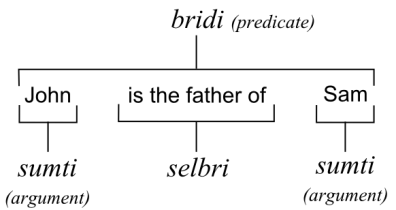
\includegraphics[width=\imgwidth,height=\imgheight,keepaspectratio=true]{media/chapter-2-diagram.png}}}}{}\end{center}
\end{minipage}

  
    In a relationship, there are a definite number of things being related. In English, for example, 
 “give” has three places: the donor, the recipient and the gift. For example:
  
\begin{longfloat}{example}{\caption[{   }]{  \label{c2e1d4}\hyperlabel{c2e1d4}  \index{give!example}  }
\label{example-random-id-DE08}\hyperlabel{example-random-id-DE08}%
}

John gives Sam the book.

\end{longfloat}
  
and
  
\begin{longfloat}{example}{\caption[{   }]{  \label{c2e1d5}\hyperlabel{c2e1d5}  \index{give!example}  }
\label{example-random-id-IBBE}\hyperlabel{example-random-id-IBBE}%
}

Sam gives John the book.

\end{longfloat}
  
mean two different things because the relative positions of 
 “John” and 
 “Sam” have been switched. Further,
  
\begin{longfloat}{example}{\caption[{   }]{  \label{c2e1d6}\hyperlabel{c2e1d6}  \index{give!example}  }
\label{example-random-id-DxbA}\hyperlabel{example-random-id-DxbA}%
}

The book gives John Sam.

\end{longfloat}
  
seems strange to us merely because the places are being filled by unorthodox arguments. The relationship expressed by 
 “give” has not changed.
  
 \index{place structure!definition of} In Lojban, each selbri has a specified number and type of arguments, known collectively as its 
 “place structure”. The simplest kind of selbri consists of a single root word, called a 
 \hyperlink{valsi-gismu}{\emph{\emph{\index{gismu}gismu}}}, and the definition in a dictionary gives the place structure explicitly. The primary task of constructing a Lojban sentence, after choosing the relationship itself, is deciding what you will use to fill in the sumti places.
  
This book uses the Lojban terms 
 \hyperlink{valsi-bridi}{\emph{\emph{\index{bridi}bridi}}}, 
 \hyperlink{valsi-sumti}{\emph{\emph{\index{sumti}sumti}}}, and 
 \hyperlink{valsi-selbri}{\emph{\emph{\index{selbri}selbri}}}, because it is best to come to understand them independently of the English associations of the corresponding words, which are only roughly similar in meaning anyhow.
  
   \index{double underscore notation convention for Quick Tour chapter} \index{underscore notation for Quick Tour chapter} \index{notation conventions!for Quick Tour chapter} The Lojban examples in this chapter (but not in the rest of the book) use a single underline (-{}-{}-{}) under each sumti, and a double underline (===) under each selbri, to help you to tell them apart.
    
\section{Pronunciation}
\label{section-pronunciation}\hyperlabel{section-pronunciation}%
    
 \index{pronunciation!quick-{}tour version} Detailed pronunciation and spelling rules are given in 
 Chapter \ref{chapter-phonology}, but what follows will keep the reader from going too far astray while digesting this chapter.
  
 \index{vowels!pronunciation of!quick-{}tour version} Lojban has six recognized vowels: 
 \emph{a}, 
 \emph{e}, 
 \emph{i}, 
 \emph{o}, 
 \emph{u} and 
 \emph{y}. The first five are roughly pronounced as 
 “a” as in 
 “father”, 
 \emph{e} as in 
 “let”, 
 \emph{i} as in 
 “machine”, 
 \emph{o} as in 
 “dome” and 
 \emph{u} as in 
 “flute”. 
 \emph{y} is pronounced as the sound called 
 “schwa”, that is, as the unstressed 
 “a” as in 
 “about” or 
 “around”.
  
 \index{consonants!pronunciation of!quick-{}tour version} Twelve consonants in Lojban are pronounced more or less as their counterparts are in English: 
 \emph{b}, 
 \emph{d}, 
 \emph{f}, 
 \emph{k}, 
 \emph{l}, 
 \emph{m}, 
 \emph{n}, 
 \emph{p}, 
 \emph{r}, 
 \emph{t}, 
 \emph{v} and 
 \emph{z}. The letter 
 \emph{c}, on the other hand is pronounced as the 
 “sh” in 
 “hush”, while 
 \emph{j} is its voiced counterpart, the sound of the 
 “s” in 
 “pleasure”. 
 \emph{g} is always pronounced as it is in 
 “gift”, never as in 
 “giant”. 
 \emph{s} is as in 
 “sell”, never as in 
 “rose”. The sound of 
 \emph{x} is not found in English in normal words. It is found as 
 “ch” in Scottish 
 “loch”, as 
 “j” in Spanish 
 “junta”, and as 
 „ch“ in German 
 „Bach“; it also appears in the English interjection 
 “yecchh!”. It gets easier to say as you practice it. The letter 
 \emph{r} can be trilled, but doesn't have to be.
  
 \index{diphthongs!pronunciation of!quick-{}tour version} The Lojban diphthongs 
 \emph{ai}, 
 \emph{ei}, 
 \emph{oi}, and 
 \emph{au} are pronounced much as in the English words 
 “sigh”, 
 “say”, 
 “boy”, and 
 “how”. Other Lojban diphthongs begin with an 
 \emph{i} pronounced like English 
 “y” (for example, 
 \emph{io} is pronounced 
 “yo”) or else with a 
 \emph{u} pronounced like English 
 “w” (for example, 
 \emph{ua} is pronounced 
 “wa”).
  
 \index{period!quick-{}tour version} \index{comma!quick-{}tour version} \index{apostrophe!quick-{}tour version} Lojban also has three 
 “semi-{}letters”: the period, the comma and the apostrophe. The period represents a glottal stop or a pause; it is a required stoppage of the flow of air in the speech stream. The apostrophe sounds just like the English letter 
  “h”. Unlike a regular consonant, it is not found at the beginning or end of a word, nor is it found adjacent to a consonant; it is only found between two vowels. The comma has no sound associated with it, and is used to separate syllables that might ordinarily run together. It is not used in this chapter.
  
 \index{stress!quick-{}tour version} Stress falls on the next to the last syllable of all words, unless that vowel is 
 \emph{y}, which is never stressed; in such words the third-{}to-{}last syllable is stressed. If a word only has one syllable, then that syllable is not stressed.
  
All Lojban words are pronounced as they are spelled: there are no silent letters.
    
\section{Words that can act as sumti}
\label{section-sumti-cmavo}\hyperlabel{section-sumti-cmavo}%
    
 \index{pro-{}sumti!quick-{}tour version} Here is a short table of single words used as sumti. This table provides examples only, not the entire set of such words, which may be found in 
 Section \ref{section-koha-summary}.
  
\begin{tabulary}{\linewidth}{LL}
{}\emph{mi}&
{}
I/me, we/us
\tabularnewline
{}\emph{do}&
{}
you
\tabularnewline
{}\emph{ti}&
{}
this, these
\tabularnewline
{}\emph{ta}&
{}
that, those
\tabularnewline
{}\emph{tu}&
{}
that far away, those far away
\tabularnewline
{}\emph{zo'e}&
{}
unspecified value (used when a sumti is unimportant or obvious)
\tabularnewline
\end{tabulary}
  
Lojban sumti are not specific as to number (singular or plural), nor gender (masculine/feminine/neutral). Such distinctions can be optionally added by methods that are beyond the scope of this chapter.
   
 \index{pointing cmavo!quick-{}tour version} The cmavo 
 \hyperlink{valsi-ti}{\emph{\emph{\index{ti}ti}}}, 
 \hyperlink{valsi-ta}{\emph{\emph{\index{ta}ta}}}, and 
 \hyperlink{valsi-tu}{\emph{\emph{\index{tu}tu}}} refer to whatever the speaker is pointing at, and should not be used to refer to things that cannot in principle be pointed at.
  
 \index{names!quick-{}tour version} Names may also be used as sumti, provided they are preceded with the word 
 \hyperlink{valsi-la}{\emph{\emph{\index{la}la}}}:
  
\begin{tabulary}{\linewidth}{LL}
{}\emph{\index{la meris.}la meris.}&
the one/ones named Mary\tabularnewline
{}\emph{\index{la djan.}la djan.}&
the one/ones named John\tabularnewline
\end{tabulary}
  
Other Lojban spelling versions are possible for names from other languages, and there are restrictions on which letters may appear in Lojban names: see 
 Section \ref{section-names} for more information.
    
\section{Some words used to indicate selbri relations}
\label{section-some-selbri}\hyperlabel{section-some-selbri}%
    
 \index{selbri list for quick tour} Here is a short table of some words used as Lojban selbri in this chapter:
  
\begin{tabulary}{\linewidth}{LL}
{}\hyperlink{valsi-vecnu}{\emph{\emph{\index{vecnu}vecnu}}}&
x1 (seller) sells x2 (goods) to x3 (buyer) for x4 (price)\tabularnewline
{}\hyperlink{valsi-tavla}{\emph{\emph{\index{tavla}tavla}}}&
x1 (talker) talks to x2 (audience) about x3 (topic) in language x4\tabularnewline
{}\hyperlink{valsi-sutra}{\emph{\emph{\index{sutra}sutra}}}&
x1 (agent) is fast at doing x2 (action)\tabularnewline
{}\hyperlink{valsi-blariho}{\emph{\emph{\index{blari'o}blari'o}}}&
x1 (object/light source) is blue-green\tabularnewline
{}\hyperlink{valsi-melbi}{\emph{\emph{\index{melbi}melbi}}}&
x1 (object/idea) is beautiful to x2 (observer) by standard x3\tabularnewline
{}\hyperlink{valsi-cutci}{\emph{\emph{\index{cutci}cutci}}}&
x1 is a shoe/boot for x2 (foot) made of x3 (material)\tabularnewline
{}\hyperlink{valsi-bajra}{\emph{\emph{\index{bajra}bajra}}}&
x1 runs on x2 (surface) using x3 (limbs) in manner x4 (gait)\tabularnewline
{}\hyperlink{valsi-klama}{\emph{\emph{\index{klama}klama}}}&
x1 goes/comes to x2 (destination) from x3 (origin point) via x4 (route) using x5 (means of transportation)\tabularnewline
{}\hyperlink{valsi-pluka}{\emph{\emph{\index{pluka}pluka}}}&
x1 pleases/is pleasing to x2 (experiencer) under conditions x3\tabularnewline
{}\hyperlink{valsi-gerku}{\emph{\emph{\index{gerku}gerku}}}&
x1 is a dog of breed x2\tabularnewline
{}\hyperlink{valsi-kurji}{\emph{\emph{\index{kurji}kurji}}}&
x1 takes care of x2\tabularnewline
{}\hyperlink{valsi-kanro}{\emph{\emph{\index{kanro}kanro}}}&
x1 is healthy by standard x2\tabularnewline
{}\hyperlink{valsi-stali}{\emph{\emph{\index{stali}stali}}}&
x1 stays/remains with x2\tabularnewline
{}\hyperlink{valsi-zarci}{\emph{\emph{\index{zarci}zarci}}}&
x1 is a market/store/shop selling x2 (products) operated by x3 (storekeeper)\tabularnewline
\end{tabulary}
  
 \index{x1!notation convention!quick-{}tour version} Each selbri (relation) has a specific rule that defines the role of each sumti in the bridi, based on its position. In the table above, that order was expressed by labeling the sumti positions as x1, x2, x3, x4, and x5.
  
 \index{words not in the dictionary} Like the table in 
 Section \ref{section-sumti-cmavo}, this table is far from complete: in fact, no complete table can exist, because Lojban allows new words to be created (in specified ways) whenever a speaker or writer finds the existing supply of words inadequate. This notion is a basic difference between Lojban (and some other languages such as German and Chinese) and English; in English, most people are very leery of using words that 
 “aren't in the dictionary”. Lojbanists are encouraged to invent new words; doing so is a major way of participating in the development of the language. 
 Chapter \ref{chapter-morphology} explains how to make new words, and 
 Chapter \ref{chapter-lujvo} explains how to give them appropriate meanings.
    
\section{Some simple Lojban bridi}
\label{section-some-simple-bridi}\hyperlabel{section-some-simple-bridi}%
    
 \index{bridi!quick-{}tour version} Let's look at a simple Lojban bridi. The place structure of the gismu 
 \hyperlink{valsi-tavla}{\emph{\emph{\index{tavla}tavla}}} is
  
\begin{longfloat}{example}{\caption[{  }]{  \label{c2e5d1}\hyperlabel{c2e5d1}  }
\label{example-random-id-5Lis}\hyperlabel{example-random-id-5Lis}%
}

x1 talks to x2 about x3 in language x4

\end{longfloat}
  
where the 
 “x” es with following numbers represent the various arguments that could be inserted at the given positions in the English sentence. For example:
  
\begin{longfloat}{example}{\caption[{   }]{  \index{engineering!example}  \label{c2e5d2}\hyperlabel{c2e5d2}  }
\label{example-random-id-3bc3}\hyperlabel{example-random-id-3bc3}%
}

John talks to Sam about engineering in Lojban.

\end{longfloat}
  
    has 
 “John” in the x1 place, 
 “Sam” in the x2 place, 
 “engineering” in the x3 place, and 
  “Lojban” in the x4 place, and could be paraphrased:
  
\begin{longfloat}{example}{\caption[{  }]{  \label{c2e5d3}\hyperlabel{c2e5d3}  }
\label{example-random-id-pVMH}\hyperlabel{example-random-id-pVMH}%
}

Talking is going on, with speaker John and listener Sam and subject matter engineering and language Lojban.

\end{longfloat}
  
The Lojban bridi corresponding to 
 Example \ref{example-random-id-5Lis} will have the form
  
\begin{longfloat}{example}{\caption[{  }]{  \label{c2e5d4}\hyperlabel{c2e5d4}  }
\label{example-random-id-k01t}\hyperlabel{example-random-id-k01t}%
}

\begin{tabulary}{\linewidth}{LLLLLL}
{}\ul{x1}&
{}
cu
&
{}\bf{tavla}&
{}\ul{x2}&
{}\ul{x3}&
{}\ul{x4}\tabularnewline
\end{tabulary}

\end{longfloat}
  
 \index{cu!use of!quick-{}tour version} \index{cu!omission of!quick-{}tour version} The word 
 \hyperlink{valsi-cu}{\emph{\emph{\index{cu}cu}}} serves as a separator between any preceding sumti and the selbri. It can often be omitted, as in the following examples.
  
\begin{longfloat}{example}{\caption[{  }]{  \label{c2e5d5}\hyperlabel{c2e5d5}  }
\label{example-random-id-k02C}\hyperlabel{example-random-id-k02C}%
}

\begin{tabulary}{\linewidth}{LLLLL}
{}\ul{mi}&
{}\bf{tavla}&
{}\ul{do}&
{}\ul{zo'e}&
{}\ul{zo'e}\tabularnewline
\multicolumn{5}{l}{
I talk to you about something in some language.
}\tabularnewline
\end{tabulary}

\end{longfloat}
  
\begin{longfloat}{example}{\caption[{  }]{  \label{c2e5d6}\hyperlabel{c2e5d6}  }
\label{example-random-id-k02u}\hyperlabel{example-random-id-k02u}%
}

\begin{tabulary}{\linewidth}{LLLLL}
{}\ul{do}&
{}\bf{tavla}&
{}\ul{mi}&
{}\ul{ta}&
{}\ul{zo'e}\tabularnewline
\multicolumn{5}{l}{
You talk to me about that thing in a language.
}\tabularnewline
\end{tabulary}

\end{longfloat}
  
\begin{longfloat}{example}{\caption[{  }]{  \label{c2e5d7}\hyperlabel{c2e5d7}  }
\label{example-random-id-k03n}\hyperlabel{example-random-id-k03n}%
}

\begin{tabulary}{\linewidth}{LLLLL}
{}\ul{mi}&
{}\bf{tavla}&
{}\ul{zo'e}&
{}\ul{tu}&
{}\ul{ti}\tabularnewline
\multicolumn{5}{l}{
I talk to someone about that thing yonder in this language.
}\tabularnewline
\end{tabulary}

\end{longfloat}
  
(
 Example \ref{example-random-id-k03n} is a bit unusual, as there is no easy way to point to a language; one might point to a copy of this book, and hope the meaning gets across!)
  
 \index{ellipsis!quick-{}tour version} When there are one or more occurrences of the cmavo 
 \hyperlink{valsi-zohe}{\emph{\emph{\index{zo'e}zo'e}}} at the end of a bridi, they may be omitted, a process called 
 “ellipsis”. 
  Example \ref{example-random-id-k02C} and 
 Example \ref{example-random-id-k02u} may be expressed thus:
  
\begin{longfloat}{example}{\caption[{  }]{  \label{c2e5d8}\hyperlabel{c2e5d8}  }
\label{example-random-id-k04J}\hyperlabel{example-random-id-k04J}%
}

\begin{tabulary}{\linewidth}{LLL}
{}\ul{mi}&
{}\bf{tavla}&
{}\ul{do}\tabularnewline
\multicolumn{3}{l}{
I talk to you (about something in some language).
}\tabularnewline
\end{tabulary}

\end{longfloat}
  
\begin{longfloat}{example}{\caption[{  }]{  \label{c2e5d9}\hyperlabel{c2e5d9}  }
\label{example-random-id-k05i}\hyperlabel{example-random-id-k05i}%
}

\begin{tabulary}{\linewidth}{LLLL}
{}\ul{do}&
{}\bf{tavla}&
{}\ul{mi}&
{}\ul{ta}\tabularnewline
\multicolumn{4}{l}{
You talk to me about that thing (in some language).
}\tabularnewline
\end{tabulary}

\end{longfloat}
  
Note that 
 Example \ref{example-random-id-k03n} is not subject to ellipsis by this direct method, as the 
  \hyperlink{valsi-zohe}{\emph{\emph{\index{zo'e}zo'e}}} in it is not at the end of the bridi.
    
\section{Variant bridi structure}
\label{section-variant-bridi-structure}\hyperlabel{section-variant-bridi-structure}%
    
 \index{sumti placement!variant!quick-{}tour version} Consider the sentence
  
\begin{longfloat}{example}{\caption[{  }]{  \label{c2e6d1}\hyperlabel{c2e6d1}  }
\label{example-random-id-k068}\hyperlabel{example-random-id-k068}%
}

\begin{tabulary}{\linewidth}{LLLLLL}
{}\ul{mi}&
{}
cu
&
{}\bf{vecnu}&
{}\ul{ti}&
{}\ul{ta}&
{}\ul{zo'e}\tabularnewline
{}\ul{seller-x1}&
{}\emph{}&
{}\bf{sells}&
{}\ul{goods-sold-x2}&
{}\ul{buyer-x3}&
{}\ul{price-x4}\tabularnewline
{}\ul{I}&
{}\emph{}&
{}\bf{sell}&
{}\ul{this}&
{}\ul{to that}&
{}\ul{for some price.}\tabularnewline
\multicolumn{6}{l}{
I sell this-{}thing/these-{}things to that-{}buyer/those-{}buyers.
}\tabularnewline
\multicolumn{6}{l}{\emph{(the price is obvious or unimportant)}}\tabularnewline
\end{tabulary}

\end{longfloat}
  
  Example \ref{example-random-id-k068} has one sumti (the x1) before the selbri. It is also possible to put more than one sumti before the selbri, without changing the order of sumti:
  
\begin{longfloat}{example}{\caption[{  }]{  \label{c2e6d2}\hyperlabel{c2e6d2}  }
\label{example-random-id-k0aR}\hyperlabel{example-random-id-k0aR}%
}

\begin{tabulary}{\linewidth}{LLLLL}
{}\ul{mi}&
{}\ul{ti}&
{}
cu
&
{}\bf{vecnu}&
{}\ul{ta}\tabularnewline
{}\ul{seller-x1}&
{}\ul{goods-sold-x2}&
{}\emph{}&
{}\bf{sells}&
{}\ul{buyer-x3}\tabularnewline
{}\ul{I}&
{}\ul{this}&
{}\emph{}&
{}\bf{sell}&
{}\ul{to that.}\tabularnewline
\multicolumn{5}{l}{\emph{(translates as stilted or poetic English)}}\tabularnewline
\multicolumn{5}{l}{
I this thing do sell to that buyer.
}\tabularnewline
\end{tabulary}

\end{longfloat}
  
\begin{longfloat}{example}{\caption[{  }]{  \label{c2e6d3}\hyperlabel{c2e6d3}  }
\label{example-random-id-k0Bm}\hyperlabel{example-random-id-k0Bm}%
}

\begin{tabulary}{\linewidth}{LLLLL}
{}\ul{mi}&
{}\ul{ti}&
{}\ul{ta}&
{}
cu
&
{}\bf{vecnu}\tabularnewline
{}\ul{seller-x1}&
{}\ul{goods-sold-x2}&
{}\ul{buyer-x3}&
{}

&
{}\bf{sells}\tabularnewline
{}\ul{I}&
{}\ul{this}&
{}\ul{to that}&
{}

&
{}\bf{sell}\tabularnewline
\multicolumn{5}{l}{\emph{(translates as stilted or poetic English)}}\tabularnewline
\multicolumn{5}{l}{
I this thing to that buyer do sell.
}\tabularnewline
\end{tabulary}

\end{longfloat}
  
  Example \ref{example-random-id-k068} through 
 Example \ref{example-random-id-k0Bm} mean the same thing. Usually, placing more than one sumti before the selbri is done for style or for emphasis on the sumti that are out-{}of-{}place from their normal position. (Native speakers of languages other than English may prefer such orders.)
  
 \index{observatives!quick-{}tour version} If there are no sumti before the selbri, then it is understood that the x1 sumti value is equivalent to 
 \hyperlink{valsi-zohe}{\emph{\emph{\index{zo'e}zo'e}}}; i.e. unimportant or obvious, and therefore not given. Any sumti after the selbri start counting from x2.
  
\begin{longfloat}{example}{\caption[{  }]{  \label{c2e6d4}\hyperlabel{c2e6d4}  }
\label{example-random-id-k0br}\hyperlabel{example-random-id-k0br}%
}

\begin{tabulary}{\linewidth}{LLLL}
{}\ul{ta}&
{}
cu
&
{}\bf{melbi}\tabularnewline
{}\ul{object/idea-x1}&
{}

&
{}\bf{is-beautiful}&
{}\emph{to someone by some standard}\tabularnewline
{}\ul{That/Those}&
{}

&
{}\bf{is/are beautiful.}\tabularnewline
\multicolumn{4}{l}{
That is beautiful.
}\tabularnewline
\multicolumn{4}{l}{
Those are beautiful.
}\tabularnewline
\end{tabulary}

\end{longfloat}
  
when the x1 is omitted, becomes:
  
\begin{longfloat}{example}{\caption[{  }]{  \label{c2e6d5}\hyperlabel{c2e6d5}  }
\label{example-random-id-k0Ch}\hyperlabel{example-random-id-k0Ch}%
}

\begin{tabulary}{\linewidth}{LLL}
{}\ul{}&
{}\bf{melbi}&
{}\emph{}\tabularnewline
{}\ul{unspecified-x1}&
{}\bf{is-beautiful}&
{}\emph{to someone by some standard}\tabularnewline
\multicolumn{3}{l}{
Beautiful!
}\tabularnewline
\multicolumn{3}{l}{
It's beautiful!
}\tabularnewline
\end{tabulary}

\end{longfloat}
  
Omitting the x1 adds emphasis to the selbri relation, which has become first in the sentence. This kind of sentence is termed an observative, because it is often used when someone first observes or takes note of the relationship, and wishes to quickly communicate it to someone else. Commonly understood English observatives include 
   “Smoke!” upon seeing smoke or smelling the odor, or 
 “Car!” to a person crossing the street who might be in danger. Any Lojban selbri can be used as an observative if no sumti appear before the selbri.
   
The word 
 \hyperlink{valsi-cu}{\emph{\emph{\index{cu}cu}}} does not occur in an observative; 
  \hyperlink{valsi-cu}{\emph{\emph{\index{cu}cu}}} is a separator, and there must be a sumti before the selbri that needs to be kept separate for 
 \hyperlink{valsi-cu}{\emph{\emph{\index{cu}cu}}} to be used. With no sumti preceding the selbri, 
 \hyperlink{valsi-cu}{\emph{\emph{\index{cu}cu}}} is not permitted. Short words like 
 \hyperlink{valsi-cu}{\emph{\emph{\index{cu}cu}}} which serve grammatical functions are called 
 \hyperlink{valsi-cmavo}{\emph{\emph{\index{cmavo}cmavo}}} in Lojban.
    
\section{Varying the order of sumti}
\label{section-order-of-sumti}\hyperlabel{section-order-of-sumti}%
    
 \index{sumti reordering!quick-{}tour version} For one reason or another you may want to change the order, placing one particular sumti at the front of the bridi. The cmavo 
 \hyperlink{valsi-se}{\emph{\emph{\index{se}se}}}, when placed before the last word of the selbri, will switch the meanings of the first and second sumti places. So
  
\begin{longfloat}{example}{\caption[{  }]{  \label{c2e7d1}\hyperlabel{c2e7d1}  }
\label{example-random-id-k0dU}\hyperlabel{example-random-id-k0dU}%
}

\begin{tabulary}{\linewidth}{LLLL}
{}\ul{mi}&
{}\bf{tavla}&
{}\ul{do}&
{}\ul{ti}\tabularnewline
\multicolumn{4}{l}{
I talk to you about this.
}\tabularnewline
\end{tabulary}

\end{longfloat}
  
has the same meaning as
  
\begin{longfloat}{example}{\caption[{  }]{  \label{c2e7d2}\hyperlabel{c2e7d2}  }
\label{example-random-id-k0eV}\hyperlabel{example-random-id-k0eV}%
}

\begin{tabulary}{\linewidth}{LLLL}
{}\ul{do}&
{}\bf{se tavla}&
{}\ul{mi}&
{}\ul{ti}\tabularnewline
\multicolumn{4}{l}{
You are talked to by me about this.
}\tabularnewline
\end{tabulary}

\end{longfloat}
  
 The cmavo 
 \hyperlink{valsi-te}{\emph{\emph{\index{te}te}}}, when used in the same location, switches the meanings of the first and the third sumti places.
  
\begin{longfloat}{example}{\caption[{  }]{  \label{c2e7d3}\hyperlabel{c2e7d3}  }
\label{example-random-id-k0FJ}\hyperlabel{example-random-id-k0FJ}%
}

\begin{tabulary}{\linewidth}{LLLL}
{}\ul{mi}&
{}\bf{tavla}&
{}\ul{do}&
{}\ul{ti}\tabularnewline
\multicolumn{4}{l}{
I talk to you about this.
}\tabularnewline
\end{tabulary}

\end{longfloat}
  
has the same meaning as
  
\begin{longfloat}{example}{\caption[{  }]{  \label{c2e7d4}\hyperlabel{c2e7d4}  }
\label{example-random-id-k0fo}\hyperlabel{example-random-id-k0fo}%
}

\begin{tabulary}{\linewidth}{LLLL}
{}\ul{ti}&
{}\bf{te tavla}&
{}\ul{do}&
{}\ul{mi}\tabularnewline
\multicolumn{4}{l}{
This is talked about to you by me.
}\tabularnewline
\end{tabulary}

\end{longfloat}
  
Note that only the first and third sumti have switched places; the second sumti has remained in the second place.
  
 The cmavo 
 \hyperlink{valsi-ve}{\emph{\emph{\index{ve}ve}}} and 
 \hyperlink{valsi-xe}{\emph{\emph{\index{xe}xe}}} switch the first and fourth sumti places, and the first and fifth sumti places, respectively. These changes in the order of places are known as 
 “conversions”, and the 
 \hyperlink{valsi-se}{\emph{\emph{\index{se}se}}}, 
 \hyperlink{valsi-te}{\emph{\emph{\index{te}te}}}, 
 \hyperlink{valsi-ve}{\emph{\emph{\index{ve}ve}}}, and 
 \hyperlink{valsi-xe}{\emph{\emph{\index{xe}xe}}} cmavo are said to convert the selbri.
  
More than one of these operators may be used on a given selbri at one time, and in such a case they are evaluated from left to right. However, in practice they are used one at a time, as there are better tools for complex manipulation of the sumti places. See 
 Chapter \ref{chapter-selbri} for details.
   
 \index{passive voice} The effect is similar to what in English is called the 
 “passive voice”. In Lojban, the converted selbri has a new place structure that is renumbered to reflect the place reversal, thus having effects when such a conversion is used in combination with other constructs such as 
   \emph{\index{le selbri [ku]}le selbri [ku]} (see 
 Section \ref{section-description-sumti}).
    
\section{The basic structure of longer utterances}
\label{section-structure-of-utterances}\hyperlabel{section-structure-of-utterances}%
    
 People don't always say just one sentence. Lojban has a specific structure for talk or writing that is longer than one sentence. The entirety of a given speech event or written text is called an utterance. The sentences (usually, but not always, bridi) in an utterance are separated by the cmavo 
 \hyperlink{valsi-niho}{\emph{\emph{\index{ni'o}ni'o}}} and 
 \hyperlink{valsi-i}{\emph{\emph{\index{i}i}}}. These correspond to a brief pause (or nothing at all) in spoken English, and the various punctuation marks like period, question mark, and exclamation mark in written English. These separators prevent the sumti at the beginning of the next sentence from being mistaken for a trailing sumti of the previous sentence.
   
The cmavo 
 \hyperlink{valsi-niho}{\emph{\emph{\index{ni'o}ni'o}}} separates paragraphs (covering different topics of discussion). In a long text or utterance, the topical structure of the text may be indicated by multiple 
 \hyperlink{valsi-niho}{\emph{\emph{\index{ni'o}ni'o}}} s, with perhaps 
 \emph{\index{ni'oni'oni'o}ni'oni'oni'o} used to indicate a chapter, 
 \emph{\index{ni'oni'o}ni'oni'o} to indicate a section, and a single 
 \hyperlink{valsi-niho}{\emph{\emph{\index{ni'o}ni'o}}} to indicate a subtopic corresponding to a single English paragraph.
  
The cmavo 
 \hyperlink{valsi-i}{\emph{\emph{\index{i}i}}} separates sentences. It is sometimes compounded with words that modify the exact meaning (the semantics) of the sentence in the context of the utterance. (The cmavo 
 \hyperlink{valsi-xu}{\emph{\emph{\index{xu}xu}}}, discussed in 
 Section \ref{section-basic-questions}, is one such word – it turns the sentence from a statement to a question about truth.) When more than one person is talking, a new speaker will usually omit the 
 \hyperlink{valsi-i}{\emph{\emph{\index{i}i}}} even though she/he may be continuing on the same topic.
  
It is still O.K. for a new speaker to say the 
 \hyperlink{valsi-i}{\emph{\emph{\index{i}i}}} before continuing; indeed, it is encouraged for maximum clarity (since it is possible that the second speaker might merely be adding words onto the end of the first speaker's sentence). A good translation for 
 \hyperlink{valsi-i}{\emph{\emph{\index{i}i}}} is the 
 “and” used in run-{}on sentences when people are talking informally: 
 “I did this, and then I did that, and ..., and ...”.
    
\section{tanru}
\label{section-basic-tanru}\hyperlabel{section-basic-tanru}%
    
 \index{tanru!quick-{}tour version} When two gismu are adjacent, the first one modifies the second, and the selbri takes its place structure from the rightmost word. Such combinations of gismu are called 
 \hyperlink{valsi-tanru}{\emph{\emph{\index{tanru}tanru}}}. For example,
  
\begin{longfloat}{example}{\caption[{  }]{  \label{c2e9d1}\hyperlabel{c2e9d1}  }
\label{example-random-id-GPcS}\hyperlabel{example-random-id-GPcS}%
}

\begin{tabulary}{\linewidth}{LL}
{}sutra&
{}tavla\tabularnewline
\end{tabulary}

\end{longfloat}
  
has the place structure
  
\begin{longfloat}{example}{\caption[{   }]{  \index{fast talker!example}   \label{c2e9d2}\hyperlabel{c2e9d2}  }
\label{example-random-id-ANfh}\hyperlabel{example-random-id-ANfh}%
}

x1 is a fast type-{}of talker to x2 about x3 in language x4

x1 talks fast to x2 about x3 in language x4

\end{longfloat}
  
    \index{tanru default grouping!quick-{}tour version} When three or more gismu are in a row, the first modifies the second, and that combined meaning modifies the third, and that combined meaning modifies the fourth, and so on. For example
  
\begin{longfloat}{example}{\caption[{  }]{  \label{c2e9d3}\hyperlabel{c2e9d3}  }
\label{example-random-id-pzS9}\hyperlabel{example-random-id-pzS9}%
}

\begin{tabulary}{\linewidth}{LLL}
{}sutra&
{}tavla&
{}cutci\tabularnewline
\end{tabulary}

\end{longfloat}
  
    has the place structure
  
\begin{longfloat}{example}{\caption[{   }]{  \index{fast-{}talker shoe!example}   \label{c2e9d4}\hyperlabel{c2e9d4}  }
\label{example-random-id-7KPn}\hyperlabel{example-random-id-7KPn}%
}

s1 is a fast-{}talker type of shoe worn by s2 of material s3

\end{longfloat}
  
That is, it is a shoe that is worn by a fast talker rather than a shoe that is fast and is also worn by a talker.
   
Note especially the use of 
 “type-{}of” as a mechanism for connecting the English translations of the two or more gismu; this convention helps the learner understand each tanru in its context. Creative interpretations are also possible, however:
  
\begin{longfloat}{example}{\caption[{   }]{  \index{runner shoe!example}   \label{c2e9d5}\hyperlabel{c2e9d5}  }
\label{example-random-id-jE94}\hyperlabel{example-random-id-jE94}%
}

\begin{tabulary}{\linewidth}{LL}
{}bajra&
{}cutci\tabularnewline
\multicolumn{2}{l}{
runner shoe
}\tabularnewline
\end{tabulary}

\end{longfloat}
  
    most probably refers to shoes suitable for runners, but might be interpreted in some imaginative instances as 
 “shoes that run (by themselves?)”. In general, however, the meaning of a tanru is determined by the literal meaning of its components, and not by any connotations or figurative meanings. Thus
  
\begin{longfloat}{example}{\caption[{  }]{  \label{c2e9d6}\hyperlabel{c2e9d6}  }
\label{example-random-id-HcV5}\hyperlabel{example-random-id-HcV5}%
}

\begin{tabulary}{\linewidth}{LL}
{}sutra&
{}tavla\tabularnewline
\multicolumn{2}{l}{
fast-{}talker
}\tabularnewline
\end{tabulary}

\end{longfloat}
  
would not necessarily imply any trickery or deception, unlike the English idiom, and a
  
\begin{longfloat}{example}{\caption[{     }]{  \index{Lepidoptera!example}  \index{butterfly!social!example}  \index{social butterfly!example}  \label{c2e9d7}\hyperlabel{c2e9d7}  }
\label{example-random-id-8umU}\hyperlabel{example-random-id-8umU}%
}

\begin{tabulary}{\linewidth}{LL}
{}jikca&
{}toldi\tabularnewline
\multicolumn{2}{l}{
social butterfly
}\tabularnewline
\end{tabulary}

\end{longfloat}
  
    must always be an insect with large brightly-{}colored wings, of the family 
 \emph{Lepidoptera}.
   
 \index{tanru!place structure of!quick-{}tour version} The place structure of a tanru is always that of the final component of the tanru. Thus, the following has the place structure of 
 \hyperlink{valsi-klama}{\emph{\emph{\index{klama}klama}}}:
  
\begin{longfloat}{example}{\caption[{  }]{  \label{c2e9d8}\hyperlabel{c2e9d8}  }
\label{example-random-id-k0FP}\hyperlabel{example-random-id-k0FP}%
}

\begin{tabulary}{\linewidth}{LLLL}
{}\ul{mi}&
{}
cu
&
{}\bf{sutra klama}&
{}\ul{la meris.}\tabularnewline
{}\ul{I}&
{}

&
{}\bf{quickly-go}&
{}\ul{to Mary.}\tabularnewline
\end{tabulary}

\end{longfloat}
  
 \index{tanru conversion!effect on place structure!quick-{}tour version} With the conversion 
 \emph{\index{se klama}se klama} as the final component of the tanru, the place structure of the entire selbri is that of 
 \emph{\index{se klama}se klama}: the x1 place is the destination, and the x2 place is the one who goes:
   
\begin{longfloat}{example}{\caption[{  }]{  \label{c2e9d9}\hyperlabel{c2e9d9}  }
\label{example-random-id-k0J1}\hyperlabel{example-random-id-k0J1}%
}

\begin{tabulary}{\linewidth}{LLLLL}
{}\ul{mi}&
{}
cu
&
{}\bf{sutra}&
{}\bf{se klama}&
{}\ul{la meris.}\tabularnewline
{}\ul{I}&
{}

&
{}\bf{quickly}&
{}\bf{am-gone-to}&
{}\ul{by Mary.}\tabularnewline
\end{tabulary}

\end{longfloat}
  
 \index{tanru!and conversion!quick-{}tour version} The following example shows that there is more to conversion than merely switching places, though:
  
\begin{longfloat}{example}{\caption[{  }]{  \label{c2e9d10}\hyperlabel{c2e9d10}  }
\label{example-random-id-k0LW}\hyperlabel{example-random-id-k0LW}%
}

\begin{tabulary}{\linewidth}{LLLL}
{}\ul{la tam.}&
{}
cu
&
{}\bf{melbi tavla}&
{}\ul{la meris.}\tabularnewline
{}\ul{Tom}&
{}

&
{}\bf{beautifully-talks}&
{}\ul{to Mary.}\tabularnewline
{}\ul{Tom}&
{}

&
{}\bf{is a beautiful-talker}&
{}\ul{to Mary.}\tabularnewline
\end{tabulary}

\end{longfloat}
  
has the place structure of 
 \hyperlink{valsi-tavla}{\emph{\emph{\index{tavla}tavla}}}, but note the two distinct interpretations.
  
Now, using conversion, we can modify the place structure order:
   
\begin{longfloat}{example}{\caption[{  }]{  \label{c2e9d11}\hyperlabel{c2e9d11}  }
\label{example-random-id-k0mh}\hyperlabel{example-random-id-k0mh}%
}

\begin{tabulary}{\linewidth}{LLLL}
{}\ul{la meris.}&
{}
cu
&
{}\bf{melbi se tavla}&
{}\ul{la tam.}\tabularnewline
{}\ul{Mary}&
{}

&
{}\bf{is beautifully-talked-to}&
{}\ul{by Tom.}\tabularnewline
{}\ul{Mary}&
{}

&
{}\bf{is a beautiful-audience}&
{}\ul{for Tom.}\tabularnewline
\end{tabulary}

\end{longfloat}
  
and we see that the modification has been changed so as to focus on Mary's role in the bridi relationship, leading to a different set of possible interpretations.
  
Note that there is no place structure change if the modifying term is converted, and so less drastic variation in possible meanings:
  
\begin{longfloat}{example}{\caption[{   }]{  \label{c2e9d12}\hyperlabel{c2e9d12}  \index{talker!example}  }
\label{example-random-id-qIv0}\hyperlabel{example-random-id-qIv0}%
}

\begin{tabulary}{\linewidth}{LLLL}
{}\ul{la tam.}&
{}
cu
&
{}\bf{tavla melbi}&
{}\ul{la meris.}\tabularnewline
{}\ul{Tom}&
{}

&
{}\bf{is talkerly-beautiful}&
{}\ul{to Mary.}\tabularnewline
\end{tabulary}

\end{longfloat}
  
\begin{longfloat}{example}{\caption[{  }]{  \label{c2e9d13}\hyperlabel{c2e9d13}  }
\label{example-random-id-qIVa}\hyperlabel{example-random-id-qIVa}%
}

\begin{tabulary}{\linewidth}{LLLL}
{}\ul{la tam.}&
{}
cu
&
{}\bf{se tavla melbi}&
{}\ul{la meris.}\tabularnewline
{}\ul{Tom}&
{}

&
{}\bf{is audiencely-beautiful}&
{}\ul{to Mary.}\tabularnewline
\end{tabulary}

\end{longfloat}
  
and we see that the manner in which Tom is seen as beautiful by Mary changes, but Tom is still the one perceived as beautiful, and Mary, the observer of beauty.
    
\section{Description sumti}
\label{section-description-sumti}\hyperlabel{section-description-sumti}%
    
   \index{descriptions!quick-{}tour version} Often we wish to talk about things other than the speaker, the listener and things we can point to. Let's say I want to talk about a talker other than 
 \hyperlink{valsi-mi}{\emph{\emph{\index{mi}mi}}}. What I want to talk about would naturally fit into the first place of 
 \hyperlink{valsi-tavla}{\emph{\emph{\index{tavla}tavla}}}. Lojban, it turns out, has an operator that pulls this first place out of a selbri and converts it to a sumti called a 
 “description sumti”. The description sumti 
 \emph{\index{le tavla ku}le tavla ku} means 
 “the talker”, and may be used wherever any sumti may be used.
  
For example,
  
\begin{longfloat}{example}{\caption[{  }]{  \label{c2e10d1}\hyperlabel{c2e10d1}  }
\label{example-random-id-k0Pj}\hyperlabel{example-random-id-k0Pj}%
}

\begin{tabulary}{\linewidth}{LLLLL}
{}\ul{mi}&
{}\bf{tavla}&
{}\ul{do}&
{}\ul{le tavla}&
{}
ku
\tabularnewline
\end{tabulary}

\end{longfloat}
  
means the same as
  
\begin{longfloat}{example}{\caption[{  }]{  \label{c2e10d2}\hyperlabel{c2e10d2}  }
\label{example-random-id-oH9T}\hyperlabel{example-random-id-oH9T}%
}

I talk to you about the talker

\end{longfloat}
  
where 
 “the talker” is presumably someone other than me, though not necessarily.
  
Similarly 
 \emph{\index{le sutra tavla ku}le sutra tavla ku} is 
 “the fast talker”, and 
  \emph{\index{le sutra te tavla ku}le sutra te tavla ku} is 
 “the fast subject of talk” or 
 “the subject of fast talk”. Which of these related meanings is understood will depend on the context in which the expression is used. The most plausible interpretation within the context will generally be assumed by a listener to be the intended one.
  
In many cases the word 
 \hyperlink{valsi-ku}{\emph{\emph{\index{ku}ku}}} may be omitted. In particular, it is never necessary in a description at the end of a sentence, so:
  
\begin{longfloat}{example}{\caption[{  }]{  \label{c2e10d3}\hyperlabel{c2e10d3}  }
\label{example-random-id-k0Q2}\hyperlabel{example-random-id-k0Q2}%
}

\begin{tabulary}{\linewidth}{LLLL}
{}\ul{mi}&
{}\bf{tavla}&
{}\ul{do}&
{}\ul{le tavla}\tabularnewline
{}\ul{I}&
{}\bf{talk-to}&
{}\ul{you}&
{}\ul{about-the talker}\tabularnewline
\end{tabulary}

\end{longfloat}
  
means exactly the same thing as 
 Example \ref{example-random-id-k0Pj}.
  
 \index{cu!need for!quick-{}tour version} There is a problem when we want to say 
 “The fast one is talking.” The 
 “obvious” translation 
 \emph{\index{le sutra tavla}le sutra tavla} turns out to mean 
 “the fast talker”, and has no selbri at all. To solve this problem we can use the word 
  \hyperlink{valsi-cu}{\emph{\emph{\index{cu}cu}}}, which so far has always been optional, in front of the selbri.
  
The word 
 \hyperlink{valsi-cu}{\emph{\emph{\index{cu}cu}}} has no meaning, and exists only to mark the beginning of the selbri within the bridi, separating it from a previous sumti. It comes before any other part of the selbri, including other cmavo like 
 \hyperlink{valsi-se}{\emph{\emph{\index{se}se}}} or 
 \hyperlink{valsi-te}{\emph{\emph{\index{te}te}}}. Thus:
  
\begin{longfloat}{example}{\caption[{  }]{  \label{c2e10d4}\hyperlabel{c2e10d4}  }
\label{example-random-id-k0QA}\hyperlabel{example-random-id-k0QA}%
}

\begin{tabulary}{\linewidth}{L}
{}\ul{le sutra tavla}\tabularnewline
{}\ul{The fast talker}\tabularnewline
\end{tabulary}

\end{longfloat}
  
\begin{longfloat}{example}{\caption[{  }]{  \label{c2e10d5}\hyperlabel{c2e10d5}  }
\label{example-random-id-k0qb}\hyperlabel{example-random-id-k0qb}%
}

\begin{tabulary}{\linewidth}{LLL}
{}\ul{le sutra}&
{}
cu
&
{}\bf{tavla}\tabularnewline
{}\ul{The fast one}&
{}

&
{}\bf{is talking.}\tabularnewline
\end{tabulary}

\end{longfloat}
  
\begin{longfloat}{example}{\caption[{  }]{  \label{c2e10d6}\hyperlabel{c2e10d6}  }
\label{example-random-id-k0Qf}\hyperlabel{example-random-id-k0Qf}%
}

\begin{tabulary}{\linewidth}{L}
{}\ul{le sutra se tavla}\tabularnewline
{}\ul{The fast talked-to one}\tabularnewline
\end{tabulary}

\end{longfloat}
  
\begin{longfloat}{example}{\caption[{  }]{  \label{c2e10d7}\hyperlabel{c2e10d7}  }
\label{example-random-id-k0ru}\hyperlabel{example-random-id-k0ru}%
}

\begin{tabulary}{\linewidth}{LLL}
{}\ul{le sutra}&
{}
cu
&
{}\bf{se tavla}\tabularnewline
{}\ul{The fast one}&
{}

&
{}\bf{is talked to.}\tabularnewline
\end{tabulary}

\end{longfloat}
  
 \index{KU selma'o!quick-{}tour version} \index{ku!quick-{}tour version} Consider the following more complex example, with two description sumti.
  
\begin{longfloat}{example}{\caption[{  }]{  \label{c2e10d8}\hyperlabel{c2e10d8}  }
\label{example-random-id-k0S1}\hyperlabel{example-random-id-k0S1}%
}

\begin{tabulary}{\linewidth}{LLLLLLL}
{}\ul{mi}&
{}
cu
&
{}\bf{tavla}&
{}\ul{le vecnu}&
{}
ku
&
{}\ul{le blari'o}&
{}
ku
\tabularnewline
{}\ul{I}&
{}

&
{}\bf{talk-to}&
{}\ul{the seller}&
{}

&
{}\ul{about the blue-green-thing.}&
{}

\tabularnewline
\end{tabulary}

\end{longfloat}
  
The sumti 
 \emph{\index{le vecnu}le vecnu} contains the selbri 
 \hyperlink{valsi-vecnu}{\emph{\emph{\index{vecnu}vecnu}}}, which has the 
 “seller” in the x1 place, and uses it in this sentence to describe a particular 
 “seller” that the speaker has in mind (one that he or she probably expects the listener will also know about). Similarly, the speaker has a particular blue-{}green thing in mind, which is described using 
 \hyperlink{valsi-le}{\emph{\emph{\index{le}le}}} to mark 
 \hyperlink{valsi-blariho}{\emph{\emph{\index{blari'o}blari'o}}}, a selbri whose first sumti is something blue-{}green.
  
It is safe to omit both occurrences of 
 \hyperlink{valsi-ku}{\emph{\emph{\index{ku}ku}}} in 
 Example \ref{example-random-id-k0S1}, and it is also safe to omit the 
 \hyperlink{valsi-cu}{\emph{\emph{\index{cu}cu}}}.
    
\section{Examples of brivla}
\label{section-some-brivla}\hyperlabel{section-some-brivla}%
    
 \index{brivla!types of!quick-{}tour version} The simplest form of selbri is an individual word. A word which may by itself express a selbri relation is called a 
 \hyperlink{valsi-brivla}{\emph{\emph{\index{brivla}brivla}}}. The three types of brivla are gismu (root words), lujvo (compounds), and fu'ivla (borrowings from other languages). All have identical grammatical uses. So far, most of our selbri have been gismu or tanru built from gismu.
   
 \index{gismu!quick-{}tour version} gismu:
  
\begin{longfloat}{example}{\caption[{  }]{  \label{c2e11d1}\hyperlabel{c2e11d1}  }
\label{example-random-id-k0SM}\hyperlabel{example-random-id-k0SM}%
}

\begin{tabulary}{\linewidth}{LLLLLLL}
{}\ul{mi}&
{}
cu
&
{}\bf{klama}&
{}\ul{ti}&
{}\ul{zo'e}&
{}\ul{zo'e}&
{}\ul{ta}\tabularnewline
{}\ul{Go-er}&
{}

&
{}\bf{goes}&
{}\ul{destination}&
{}\ul{origin}&
{}\ul{route}&
{}\ul{means.}\tabularnewline
\multicolumn{7}{l}{
I go here (to this) using that means (from somewhere via some route).
}\tabularnewline
\end{tabulary}

\end{longfloat}
  
 \index{lujvo!quick-{}tour version} lujvo:
  
\begin{longfloat}{example}{\caption[{  }]{  \label{c2e11d2}\hyperlabel{c2e11d2}  }
\label{example-random-id-k0SR}\hyperlabel{example-random-id-k0SR}%
}

\begin{tabulary}{\linewidth}{LLL}
{}\ul{ta}&
{}
cu
&
{}\bf{blari'o}\tabularnewline
{}\ul{That}&
{}

&
{}\bf{is-blue-green.}\tabularnewline
\end{tabulary}

\end{longfloat}
  
 \index{fu'ivla!quick-{}tour version} fu'ivla:
  
\begin{longfloat}{example}{\caption[{  }]{  \label{c2e11d3}\hyperlabel{c2e11d3}  }
\label{example-random-id-k0Tj}\hyperlabel{example-random-id-k0Tj}%
}

\begin{tabulary}{\linewidth}{LLL}
{}\ul{ti}&
{}
cu
&
{}\bf{djarspageti}\tabularnewline
{}\ul{This}&
{}

&
{}\bf{is-spaghetti.}\tabularnewline
\end{tabulary}

\end{longfloat}
  
 \index{cmavo as selbri!quick-{}tour version} Some cmavo may also serve as selbri, acting as variables that stand for another selbri. The most commonly used of these is 
 \hyperlink{valsi-gohi}{\emph{\emph{\index{go'i}go'i}}}, which represents the main bridi of the previous Lojban sentence, with any new sumti or other sentence features being expressed replacing the previously expressed ones. Thus, in this context:
  
\begin{longfloat}{example}{\caption[{  }]{  \label{c2e11d4}\hyperlabel{c2e11d4}  }
\label{example-random-id-k0UC}\hyperlabel{example-random-id-k0UC}%
}

\begin{tabulary}{\linewidth}{LLL}
{}\ul{ta}&
{}
cu
&
{}\bf{go'i}\tabularnewline
{}\ul{That}&
{}

&
{}\bf{too/same-as-last selbri.}\tabularnewline
\multicolumn{3}{l}{
That (is spaghetti), too.
}\tabularnewline
\end{tabulary}

\end{longfloat}
    
\section[{The sumti di'u and la'e di'u}]{The sumti 
 \hyperlink{valsi-dihu}{\emph{\emph{\index{di'u}di'u}}} and 
 \emph{\index{la'e di'u}la'e di'u}}
\label{section-dihu-and-lahe-dihu}\hyperlabel{section-dihu-and-lahe-dihu}%
    
 \index{reference!quick-{}tour version} In English, I might say 
 “The dog is beautiful”, and you might reply 
 “This pleases me.” How do you know what 
  “this” refers to? Lojban uses different expressions to convey the possible meanings of the English:
  
\begin{longfloat}{example}{\caption[{   }]{  \index{beautiful dog!example}  \label{c2e12d1}\hyperlabel{c2e12d1}  }
\label{example-random-id-k0wB}\hyperlabel{example-random-id-k0wB}%
}

\begin{tabulary}{\linewidth}{LLLL}
{}\ul{le gerku}&
{}
ku
&
{}
cu
&
{}\bf{melbi}\tabularnewline
\multicolumn{4}{l}{
The dog is beautiful.
}\tabularnewline
\end{tabulary}

\end{longfloat}
  
The following three sentences all might translate as 
 “This pleases me.”
   
\begin{longfloat}{example}{\caption[{  }]{  \label{c2e12d2}\hyperlabel{c2e12d2}  }
\label{example-random-id-k0wS}\hyperlabel{example-random-id-k0wS}%
}

\begin{tabulary}{\linewidth}{LLLL}
{}\ul{ti}&
{}
cu
&
{}\bf{pluka}&
{}\ul{mi}\tabularnewline
\multicolumn{4}{l}{
This (the dog) pleases me.
}\tabularnewline
\end{tabulary}

\end{longfloat}
  
\begin{longfloat}{example}{\caption[{  }]{  \label{c2e12d3}\hyperlabel{c2e12d3}  }
\label{example-random-id-k0yC}\hyperlabel{example-random-id-k0yC}%
}

\begin{tabulary}{\linewidth}{LLLL}
{}\ul{di'u}&
{}
cu
&
{}\bf{pluka}&
{}\ul{mi}\tabularnewline
\multicolumn{4}{l}{
This (the last sentence) pleases me (perhaps because it is grammatical or sounds nice).
}\tabularnewline
\end{tabulary}

\end{longfloat}
  
\begin{longfloat}{example}{\caption[{  }]{  \label{c2e12d4}\hyperlabel{c2e12d4}  }
\label{example-random-id-k0YS}\hyperlabel{example-random-id-k0YS}%
}

\begin{tabulary}{\linewidth}{LLLL}
{}\ul{la'e di'u}&
{}
cu
&
{}\bf{pluka}&
{}\ul{mi}\tabularnewline
\multicolumn{4}{l}{
This (the meaning of the last sentence; i.e. that the dog is beautiful) pleases me.
}\tabularnewline
\end{tabulary}

\end{longfloat}
  
 \index{pleases}  Example \ref{example-random-id-k0YS} uses one sumti to point to or refer to another by inference. It is common to write 
 \hyperlink{valsi-lahedihu}{\emph{\emph{\index{la'edi'u}la'edi'u}}} as a single word; it is used more often than 
  \hyperlink{valsi-dihu}{\emph{\emph{\index{di'u}di'u}}} by itself.
    
\section{Possession}
\label{section-possession}\hyperlabel{section-possession}%
    
 \index{possession!quick-{}tour version}  “Possession” refers to the concept of specifying an object by saying who it belongs to (or with). A full explanation of Lojban possession is given in 
 Chapter \ref{chapter-relative-clauses}. A simple means of expressing possession, however, is to place a sumti representing the possessor of an object within the description sumti that refers to the object: specifically, between the 
 \hyperlink{valsi-le}{\emph{\emph{\index{le}le}}} and the selbri of the description:
  
\begin{longfloat}{example}{\caption[{  }]{  \label{c2e13d1}\hyperlabel{c2e13d1}  }
\label{example-random-id-k0zY}\hyperlabel{example-random-id-k0zY}%
}

\begin{tabulary}{\linewidth}{LLL}
{}\ul{le mi gerku}&
{}
cu
&
{}\bf{sutra}\tabularnewline
{}\ul{The of-me dog}&
{}

&
{}\bf{is fast.}\tabularnewline
\multicolumn{3}{l}{
My dog is fast.
}\tabularnewline
\end{tabulary}

\end{longfloat}
  
 \index{possession not ownership!quick-{}tour version} In Lojban, possession doesn't necessarily mean ownership: one may 
 “possess” a chair simply by sitting on it, even though it actually belongs to someone else. English uses possession casually in the same way, but also uses it to refer to actual ownership or even more intimate relationships: 
 “my arm” doesn't mean 
 “some arm I own” but rather 
 “the arm that is part of my body”. Lojban has methods of specifying all these different kinds of possession precisely and easily.
    
\section{Vocatives and commands}
\label{section-vocatives-and-commands}\hyperlabel{section-vocatives-and-commands}%
     
 \index{vocatives!quick-{}tour version} You may call someone's attention to the fact that you are addressing them by using 
 \hyperlink{valsi-doi}{\emph{\emph{\index{doi}doi}}} followed by their name. The sentence
  
\begin{longfloat}{example}{\caption[{  }]{  \label{c2e14d1}\hyperlabel{c2e14d1}  }
\label{example-random-id-ahVb}\hyperlabel{example-random-id-ahVb}%
}

\begin{tabulary}{\linewidth}{LL}
{}doi&
{}djan.\tabularnewline
\end{tabulary}

\end{longfloat}
  
means 
 “Oh, John, I'm talking to you”. It also has the effect of setting the value of 
 \hyperlink{valsi-do}{\emph{\emph{\index{do}do}}}; 
 \hyperlink{valsi-do}{\emph{\emph{\index{do}do}}} now refers to 
 “John” until it is changed in some way in the conversation. Note that 
 Example \ref{example-random-id-ahVb} is not a bridi, but it is a legitimate Lojban sentence nevertheless; it is known as a 
 “vocative phrase”.
   
 Other cmavo can be used instead of 
 \hyperlink{valsi-doi}{\emph{\emph{\index{doi}doi}}} in a vocative phrase, with a different significance. For example, the cmavo 
  \hyperlink{valsi-coi}{\emph{\emph{\index{coi}coi}}} means 
 “hello” and 
 \hyperlink{valsi-coho}{\emph{\emph{\index{co'o}co'o}}} means 
 “good-{}bye”. Either word may stand alone, they may follow one another, or either may be followed by a pause and a name. (Vocative phrases with 
 \hyperlink{valsi-doi}{\emph{\emph{\index{doi}doi}}} do not need a pause before the name.)
  
\begin{longfloat}{example}{\caption[{  }]{  \label{c2e14d2}\hyperlabel{c2e14d2}  }
\label{example-random-id-qIWX}\hyperlabel{example-random-id-qIWX}%
}

\begin{tabulary}{\linewidth}{LL}
{}coi.&
{}djan.\tabularnewline
\multicolumn{2}{l}{
Hello, John.
}\tabularnewline
\end{tabulary}

\end{longfloat}
  
\begin{longfloat}{example}{\caption[{  }]{  \label{c2e14d3}\hyperlabel{c2e14d3}  }
\label{example-random-id-qIxE}\hyperlabel{example-random-id-qIxE}%
}

\begin{tabulary}{\linewidth}{LL}
{}co'o.&
{}djan.\tabularnewline
\multicolumn{2}{l}{
Good-{}bye, John.
}\tabularnewline
\end{tabulary}

\end{longfloat}
  
 \index{imperatives!quick-{}tour version} \index{commands!quick-{}tour version} Commands are expressed in Lojban by a simple variation of the main bridi structure. If you say
  
\begin{longfloat}{example}{\caption[{  }]{  \label{c2e14d4}\hyperlabel{c2e14d4}  }
\label{example-random-id-k11I}\hyperlabel{example-random-id-k11I}%
}

\begin{tabulary}{\linewidth}{LL}
{}\ul{do}&
{}\bf{tavla}\tabularnewline
{}\ul{You}&
{}\bf{are-talking.}\tabularnewline
\end{tabulary}

\end{longfloat}
  
you are simply making a statement of fact. In order to issue a command in Lojban, substitute the word 
 \hyperlink{valsi-ko}{\emph{\emph{\index{ko}ko}}} for 
 \hyperlink{valsi-do}{\emph{\emph{\index{do}do}}}. The bridi
  
\begin{longfloat}{example}{\caption[{   }]{  \index{Talk"!!example}  \label{c2e14d5}\hyperlabel{c2e14d5}  }
\label{example-random-id-k11z}\hyperlabel{example-random-id-k11z}%
}

\begin{tabulary}{\linewidth}{LL}
{}\ul{ko}&
{}\bf{tavla}\tabularnewline
\end{tabulary}

\end{longfloat}
  
    instructs the listener to do whatever is necessary to make 
 Example \ref{example-random-id-k11I} true; it means 
 “Talk!” Other examples:
  
\begin{longfloat}{example}{\caption[{  }]{  \label{c2e14d6}\hyperlabel{c2e14d6}  }
\label{example-random-id-k13h}\hyperlabel{example-random-id-k13h}%
}

\begin{tabulary}{\linewidth}{LL}
{}\ul{ko}&
{}\bf{sutra}\tabularnewline
\multicolumn{2}{l}{
Be fast!
}\tabularnewline
\end{tabulary}

\end{longfloat}
  
The 
 \hyperlink{valsi-ko}{\emph{\emph{\index{ko}ko}}} need not be in the x1 place, but rather can occur anywhere a sumti is allowed, leading to possible Lojban commands that are very unlike English commands:
   
\begin{longfloat}{example}{\caption[{  }]{  \label{c2e14d7}\hyperlabel{c2e14d7}  }
\label{example-random-id-k14j}\hyperlabel{example-random-id-k14j}%
}

\begin{tabulary}{\linewidth}{LLL}
{}\ul{mi}&
{}\bf{tavla}&
{}\ul{ko}\tabularnewline
\multicolumn{3}{l}{
Be talked to by me.
}\tabularnewline
\multicolumn{3}{l}{
Let me talk to you.
}\tabularnewline
\end{tabulary}

\end{longfloat}
  
The cmavo 
 \hyperlink{valsi-ko}{\emph{\emph{\index{ko}ko}}} can fill any appropriate sumti place, and can be used as often as is appropriate for the selbri:
  
\begin{longfloat}{example}{\caption[{   }]{  \index{Take care"!!example}  \label{c2e14d8}\hyperlabel{c2e14d8}  }
\label{example-random-id-k14X}\hyperlabel{example-random-id-k14X}%
}

\begin{tabulary}{\linewidth}{LLL}
{}\ul{ko}&
{}\bf{kurji}&
{}\ul{ko}\tabularnewline
\end{tabulary}

\end{longfloat}
  
and
  
\begin{longfloat}{example}{\caption[{  }]{  \label{c2e14d9}\hyperlabel{c2e14d9}  }
\label{example-random-id-k15M}\hyperlabel{example-random-id-k15M}%
}

\begin{tabulary}{\linewidth}{LLL}
{}\ul{ko}&
{}\ul{ko}&
{}\bf{kurji}\tabularnewline
\end{tabulary}

\end{longfloat}
  
    both mean 
 “You take care of you” and 
 “Be taken care of by you”, or to put it colloquially, 
 “Take care of yourself”.
    
\section{Questions}
\label{section-basic-questions}\hyperlabel{section-basic-questions}%
    
 \index{questions!quick-{}tour version} There are many kinds of questions in Lojban: full explanations appear in 
 Section \ref{section-questions-and-answers} and in various other chapters throughout the book. In this chapter, we will introduce three kinds: sumti questions, selbri questions, and yes/no questions.
    
 \index{sumti questions!quick-{}tour version} \index{questions!quick-{}tour version} The cmavo 
 \hyperlink{valsi-ma}{\emph{\emph{\index{ma}ma}}} is used to create a sumti question: it indicates that the speaker wishes to know the sumti which should be placed at the location of the 
 \hyperlink{valsi-ma}{\emph{\emph{\index{ma}ma}}} to make the bridi true. It can be translated as 
 “Who?” or 
 “What?” in most cases, but also serves for 
 “When?”, 
 “Where?”, and 
 “Why?” when used in sumti places that express time, location, or cause. For example:
  
\begin{longfloat}{example}{\caption[{  }]{  \label{c2e15d1}\hyperlabel{c2e15d1}  }
\label{example-random-id-k161}\hyperlabel{example-random-id-k161}%
}

\begin{tabulary}{\linewidth}{LLLL}
{}\ul{ma}&
{}\bf{tavla}&
{}\ul{do}&
{}\ul{mi}\tabularnewline
{}\ul{Who?}&
{}\bf{talks}&
{}\ul{to-you}&
{}\ul{about-me.}\tabularnewline
\multicolumn{4}{l}{
Who is talking to you about me?
}\tabularnewline
\end{tabulary}

\end{longfloat}
  
The listener can reply by simply stating a sumti:
  
\begin{longfloat}{example}{\caption[{  }]{  \label{c2e15d2}\hyperlabel{c2e15d2}  }
\label{example-random-id-k1Aa}\hyperlabel{example-random-id-k1Aa}%
}

\begin{tabulary}{\linewidth}{L}
{}\ul{la djan.}\tabularnewline
\multicolumn{1}{l}{
John (is talking to you about me).
}\tabularnewline
\end{tabulary}

\end{longfloat}
  
Like 
 \hyperlink{valsi-ko}{\emph{\emph{\index{ko}ko}}}, 
 \hyperlink{valsi-ma}{\emph{\emph{\index{ma}ma}}} can occur in any position where a sumti is allowed, not just in the first position:
  
\begin{longfloat}{example}{\caption[{  }]{  \label{c2e15d3}\hyperlabel{c2e15d3}  }
\label{example-random-id-k1aE}\hyperlabel{example-random-id-k1aE}%
}

\begin{tabulary}{\linewidth}{LLLL}
{}\ul{do}&
{}
cu
&
{}\bf{tavla}&
{}\ul{ma}\tabularnewline
{}\ul{You}&
{}

&
{}\bf{talk}&
{}\ul{to what/whom?}\tabularnewline
\end{tabulary}

\end{longfloat}
  
A 
 \hyperlink{valsi-ma}{\emph{\emph{\index{ma}ma}}} can also appear in multiple sumti positions in one sentence, in effect asking several questions at once.
  
\begin{longfloat}{example}{\caption[{  }]{  \label{c2e15d4}\hyperlabel{c2e15d4}  }
\label{example-random-id-k1dc}\hyperlabel{example-random-id-k1dc}%
}

\begin{tabulary}{\linewidth}{LLLL}
{}\ul{ma}&
{}
cu
&
{}\bf{tavla}&
{}\ul{ma}\tabularnewline
{}\ul{What/Who}&
{}

&
{}\bf{talks}&
{}\ul{to what/whom?}\tabularnewline
\end{tabulary}

\end{longfloat}
  
 \index{separate questions!quick-{}tour version} The two separate 
 \hyperlink{valsi-ma}{\emph{\emph{\index{ma}ma}}} positions ask two separate questions, and can therefore be answered with different values in each sumti place.
   
 \index{bridi questions!quick-{}tour version} \index{selbri questions!quick-{}tour version} The cmavo 
 \hyperlink{valsi-mo}{\emph{\emph{\index{mo}mo}}} is the selbri analogue of 
 \hyperlink{valsi-ma}{\emph{\emph{\index{ma}ma}}}. It asks the respondent to provide a selbri that would be a true relation if inserted in place of the 
 \hyperlink{valsi-mo}{\emph{\emph{\index{mo}mo}}}:
  
\begin{longfloat}{example}{\caption[{  }]{  \label{c2e15d5}\hyperlabel{c2e15d5}  }
\label{example-random-id-k1DE}\hyperlabel{example-random-id-k1DE}%
}

\begin{tabulary}{\linewidth}{LLL}
{}\ul{do}&
{}
cu
&
{}\bf{mo}\tabularnewline
{}\ul{You}&
{}

&
{}\bf{are-what/do-what?}\tabularnewline
\end{tabulary}

\end{longfloat}
  
A 
 \hyperlink{valsi-mo}{\emph{\emph{\index{mo}mo}}} may be used anywhere a brivla or other selbri might. Keep this in mind for later examples. Unfortunately, by itself, 
 \hyperlink{valsi-mo}{\emph{\emph{\index{mo}mo}}} is a very non-{}specific question. The response to the question in 
 Example \ref{example-random-id-k1DE} could be:
  
\begin{longfloat}{example}{\caption[{  }]{  \label{c2e15d6}\hyperlabel{c2e15d6}  }
\label{example-random-id-k1DR}\hyperlabel{example-random-id-k1DR}%
}

\begin{tabulary}{\linewidth}{LLL}
{}\ul{mi}&
{}
cu
&
{}\bf{melbi}\tabularnewline
\multicolumn{3}{l}{
I am beautiful.
}\tabularnewline
\end{tabulary}

\end{longfloat}
  
or:
  
\begin{longfloat}{example}{\caption[{  }]{  \label{c2e15d7}\hyperlabel{c2e15d7}  }
\label{example-random-id-k1gh}\hyperlabel{example-random-id-k1gh}%
}

\begin{tabulary}{\linewidth}{LLL}
{}\ul{mi}&
{}
cu
&
{}\bf{tavla}\tabularnewline
\multicolumn{3}{l}{
I talk.
}\tabularnewline
\end{tabulary}

\end{longfloat}
  
 \index{speaker-{}listener cooperation} Clearly, 
 \hyperlink{valsi-mo}{\emph{\emph{\index{mo}mo}}} requires some cooperation between the speaker and the respondent to ensure that the right question is being answered. If context doesn't make the question specific enough, the speaker must ask the question more specifically using a more complex construction such as a tanru (see 
 Section \ref{section-basic-tanru}).
  
It is perfectly permissible for the respondent to fill in other unspecified places in responding to a 
 \hyperlink{valsi-mo}{\emph{\emph{\index{mo}mo}}} question. Thus, the respondent in 
 Example \ref{example-random-id-k1gh} could have also specified an audience, a topic, and/or a language in the response.
  
 \index{yes/no questions!quick-{}tour version} Finally, we must consider questions that can be answered 
 “Yes” or 
 “No”, such as
  
\begin{longfloat}{example}{\caption[{  }]{  \label{c2e15d8}\hyperlabel{c2e15d8}  }
\label{example-random-id-fVMN}\hyperlabel{example-random-id-fVMN}%
}

Are you talking to me?

\end{longfloat}
  
Like all yes-{}or-{}no questions in English, 
 Example \ref{example-random-id-fVMN} may be reformulated as
  
\begin{longfloat}{example}{\caption[{  }]{  \label{c2e15d9}\hyperlabel{c2e15d9}  }
\label{example-random-id-648w}\hyperlabel{example-random-id-648w}%
}

Is it true that you are talking to me?

\end{longfloat}
  
 In Lojban we have a word that asks precisely that question in precisely the same way. The cmavo 
 \hyperlink{valsi-xu}{\emph{\emph{\index{xu}xu}}}, when placed in front of a bridi, asks whether that bridi is true as stated. So
  
\begin{longfloat}{example}{\caption[{  }]{  \label{c2e15d10}\hyperlabel{c2e15d10}  }
\label{example-random-id-k1gp}\hyperlabel{example-random-id-k1gp}%
}

\begin{tabulary}{\linewidth}{LLLL}
{}\emph{xu}&
{}\ul{do}&
{}\bf{tavla}&
{}\ul{mi}\tabularnewline
{}\emph{Is-{}it-{}true-{}that}&
{}\ul{you}&
{}\bf{are-talking}&
{}\ul{to-me?}\tabularnewline
\end{tabulary}

\end{longfloat}
  
is the Lojban translation of 
 Example \ref{example-random-id-fVMN}.
  
 \index{affirmative answer!quick-{}tour version} \index{go'i with xu!quick-{}tour version} The answer 
 “Yes” may be given by simply restating the bridi without the 
 \hyperlink{valsi-xu}{\emph{\emph{\index{xu}xu}}} question word. Lojban has a shorthand for doing this with the word 
 \hyperlink{valsi-gohi}{\emph{\emph{\index{go'i}go'i}}}, mentioned in 
 Section \ref{section-some-brivla}. Instead of a negative answer, the bridi may be restated in such a way as to make it true. If this can be done by substituting sumti, it may be done with 
  \hyperlink{valsi-gohi}{\emph{\emph{\index{go'i}go'i}}} as well. For example:
  
\begin{longfloat}{example}{\caption[{   }]{  \index{healthy!example}  \label{c2e15d11}\hyperlabel{c2e15d11}  }
\label{example-random-id-k1gU}\hyperlabel{example-random-id-k1gU}%
}

\begin{tabulary}{\linewidth}{LLL}
{}\emph{xu}&
{}\ul{do}&
{}\bf{kanro}\tabularnewline
\multicolumn{3}{l}{
Are you healthy?
}\tabularnewline
\end{tabulary}

\end{longfloat}
  
    can be answered with
  
\begin{longfloat}{example}{\caption[{   }]{  \index{healthy!example}  \label{c2e15d12}\hyperlabel{c2e15d12}  }
\label{example-random-id-k1iE}\hyperlabel{example-random-id-k1iE}%
}

\begin{tabulary}{\linewidth}{LL}
{}\ul{mi}&
{}\bf{kanro}\tabularnewline
\multicolumn{2}{l}{
I am healthy.
}\tabularnewline
\end{tabulary}

\end{longfloat}
  
or
  
\begin{longfloat}{example}{\caption[{   }]{  \index{healthy!example}  \label{c2e15d13}\hyperlabel{c2e15d13}  }
\label{example-random-id-k1JT}\hyperlabel{example-random-id-k1JT}%
}

\begin{tabulary}{\linewidth}{L}
{}\bf{go'i}\tabularnewline
\multicolumn{1}{l}{
I am healthy.
}\tabularnewline
\end{tabulary}

\end{longfloat}
  
       (Note that 
 \hyperlink{valsi-do}{\emph{\emph{\index{do}do}}} to the questioner is 
 \hyperlink{valsi-mi}{\emph{\emph{\index{mi}mi}}} to the respondent.)
 
  
or
  
\begin{longfloat}{example}{\caption[{   }]{  \index{healthy!example}  \label{c2e15d14}\hyperlabel{c2e15d14}  }
\label{example-random-id-k1jY}\hyperlabel{example-random-id-k1jY}%
}

\begin{tabulary}{\linewidth}{LLL}
{}\ul{le tavla}&
{}
cu
&
{}\bf{kanro}\tabularnewline
\multicolumn{3}{l}{
The talker is healthy.
}\tabularnewline
\end{tabulary}

\end{longfloat}
  
or
  
\begin{longfloat}{example}{\caption[{   }]{  \index{healthy!example}  \label{c2e15d15}\hyperlabel{c2e15d15}  }
\label{example-random-id-k1LE}\hyperlabel{example-random-id-k1LE}%
}

\begin{tabulary}{\linewidth}{LLL}
{}\ul{le tavla}&
{}
cu
&
{}\bf{go'i}\tabularnewline
\multicolumn{3}{l}{
The talker is healthy.
}\tabularnewline
\end{tabulary}

\end{longfloat}
  
 \index{negative answer!quick-{}tour version} A general negative answer may be given by 
  \emph{\index{na go'i}na go'i}. 
 \hyperlink{valsi-na}{\emph{\emph{\index{na}na}}} may be placed before any selbri (but after the 
 \hyperlink{valsi-cu}{\emph{\emph{\index{cu}cu}}}). It is equivalent to stating 
 “It is not true that ...” before the bridi. It does not imply that anything else is true or untrue, only that that specific bridi is not true. More details on negative statements are available in 
 Chapter \ref{chapter-negation}.
    
\section{Indicators}
\label{section-attitudinals}\hyperlabel{section-attitudinals}%
    
 \index{interjections!quick-{}tour version} \index{attitudinal indicators!quick-{}tour version} \index{indicators!quick-{}tour version} Different cultures express emotions and attitudes with a variety of intonations and gestures that are not usually included in written language. Some of these are available in some languages as interjections (i.e. Aha!, Oh no!, Ouch!, Aahh!, etc.), but they vary greatly from culture to culture.
    
Lojban has a group of cmavo known as 
 “attitudinal indicators” which specifically covers this type of commentary on spoken statements. They are both written and spoken, but require no specific intonation or gestures. Grammatically they are very simple: one or more attitudinals at the beginning of a bridi apply to the entire bridi; anywhere else in the bridi they apply to the word immediately to the left. For example:
   
\begin{longfloat}{example}{\caption[{  }]{  \label{c2e16d1}\hyperlabel{c2e16d1}  }
\label{example-random-id-k1LH}\hyperlabel{example-random-id-k1LH}%
}

\begin{tabulary}{\linewidth}{LLLL}
{}\emph{.ie}&
{}\ul{mi}&
{}
cu
&
{}\bf{klama}\tabularnewline
{}\emph{Agreement!}&
{}\ul{I}&
{}

&
{}\bf{go.}\tabularnewline
\multicolumn{4}{l}{
Yep! I'll go.
}\tabularnewline
\end{tabulary}

\end{longfloat}
  
\begin{longfloat}{example}{\caption[{  }]{  \label{c2e16d2}\hyperlabel{c2e16d2}  }
\label{example-random-id-k1mS}\hyperlabel{example-random-id-k1mS}%
}

\begin{tabulary}{\linewidth}{LLLL}
{}\emph{.ei}&
{}\ul{mi}&
{}
cu
&
{}\bf{klama}\tabularnewline
{}\emph{Obligation!}&
{}\ul{I}&
{}

&
{}\bf{go.}\tabularnewline
\multicolumn{4}{l}{
I should go.
}\tabularnewline
\end{tabulary}

\end{longfloat}
  
\begin{longfloat}{example}{\caption[{  }]{  \label{c2e16d3}\hyperlabel{c2e16d3}  }
\label{example-random-id-k1pF}\hyperlabel{example-random-id-k1pF}%
}

\begin{tabulary}{\linewidth}{LLLLLL}
{}\ul{mi}&
{}
cu
&
{}\bf{klama}&
{}\ul{le melbi}&
{}\emph{.ui}&
{}
ku
\tabularnewline
{}\ul{I}&
{}

&
{}\bf{go}&
{}\ul{to-the beautiful-thing}&
{}\emph{and I am happy because it is the beautiful thing I'm going to}&
{}

\tabularnewline
\end{tabulary}

\end{longfloat}
  
 \index{but/and equivalence} \index{metalinguistic words!quick-{}tour version} \index{discursives!quick-{}tour version} Not all indicators indicate attitudes. Discursives, another group of cmavo with the same grammatical rules as attitudinal indicators, allow free expression of certain kinds of commentary about the main utterances. Using discursives allows a clear separation of these so-{}called 
  “metalinguistic” features from the underlying statements and logical structure. By comparison, the English words 
  “but” and 
 “also”, which discursively indicate contrast or an added weight of example, are logically equivalent to 
 “and”, which does not have a discursive content. The average English-{}speaker does not think about, and may not even realize, the paradoxical idea that 
 “but” basically means 
 “and”.
  
\begin{longfloat}{example}{\caption[{  }]{  \label{c2e16d4}\hyperlabel{c2e16d4}  }
\label{example-random-id-k1Rd}\hyperlabel{example-random-id-k1Rd}%
}

\begin{tabulary}{\linewidth}{LLLLLLL}
{}\ul{mi}&
{}
cu
&
{}\bf{klama}&
{}\emph{.i}&
{}\ul{do}&
{}
cu
&
{}\bf{stali}\tabularnewline
{}\ul{I}&
{}

&
{}\bf{go.}&
{}\emph{}&
{}\ul{You}&
{}

&
{}\bf{stay.}\tabularnewline
\end{tabulary}

\end{longfloat}
  
\begin{longfloat}{example}{\caption[{  }]{  \label{c2e16d5}\hyperlabel{c2e16d5}  }
\label{example-random-id-k1Rv}\hyperlabel{example-random-id-k1Rv}%
}

\begin{tabulary}{\linewidth}{LLLLLLLLL}
{}\ul{mi}&
{}
cu
&
{}\bf{klama}&
{}\emph{.i}&
{}\emph{ji'a}&
{}\ul{do}&
{}
cu
&
{}\bf{stali}\tabularnewline
{}\ul{I}&
{}

&
{}\bf{go.}&
{}\emph{}&
{}\emph{In addition,}&
{}\ul{you}&
{}

&
{}\bf{stay.}&
{}\emph{added weight}\tabularnewline
\end{tabulary}

\end{longfloat}
  
\begin{longfloat}{example}{\caption[{  }]{  \label{c2e16d6}\hyperlabel{c2e16d6}  }
\label{example-random-id-k1sb}\hyperlabel{example-random-id-k1sb}%
}

\begin{tabulary}{\linewidth}{LLLLLLLLL}
{}\ul{mi}&
{}
cu
&
{}\bf{klama}&
{}\emph{.i}&
{}\emph{ku'i}&
{}\ul{do}&
{}
cu
&
{}\bf{stali}\tabularnewline
{}\ul{I}&
{}

&
{}\bf{go.}&
{}\emph{}&
{}\emph{However,}&
{}\ul{you}&
{}

&
{}\bf{stay.}&
{}\emph{contrast}\tabularnewline
\end{tabulary}

\end{longfloat}
  
 \index{evidentials!quick-{}tour version} Another group of indicators are called 
 “evidentials”. Evidentials show the speaker's relationship to the statement, specifically how the speaker came to make the statement. These include 
   \hyperlink{valsi-zaha}{\emph{\emph{\index{za'a}za'a}}} (I directly observe the relationship), 
  \hyperlink{valsi-pehi}{\emph{\emph{\index{pe'i}pe'i}}} (I believe that the relationship holds), 
  \hyperlink{valsi-ruha}{\emph{\emph{\index{ru'a}ru'a}}} (I postulate the relationship), and others. Many American Indian languages use this kind of words.
   
\begin{longfloat}{example}{\caption[{  }]{  \label{c2e16d7}\hyperlabel{c2e16d7}  }
\label{example-random-id-k1uT}\hyperlabel{example-random-id-k1uT}%
}

\begin{tabulary}{\linewidth}{LLLL}
{}\emph{pe'i}&
{}\ul{do}&
{}
cu
&
{}\bf{melbi}\tabularnewline
{}\emph{I opine!}&
{}\ul{You}&
{}

&
{}\bf{are beautiful.}\tabularnewline
\end{tabulary}

\end{longfloat}
  
\begin{longfloat}{example}{\caption[{  }]{  \label{c2e16d8}\hyperlabel{c2e16d8}  }
\label{example-random-id-k1Xs}\hyperlabel{example-random-id-k1Xs}%
}

\begin{tabulary}{\linewidth}{LLLL}
{}\emph{za'a}&
{}\ul{do}&
{}
cu
&
{}\bf{melbi}\tabularnewline
{}\emph{I directly observe!}&
{}\ul{You}&
{}

&
{}\bf{are beautiful.}\tabularnewline
\end{tabulary}

\end{longfloat}
    
\section{Tenses}
\label{section-tenses}\hyperlabel{section-tenses}%
    
 \index{time tenses!quick-{}tour version} \index{tenses!quick-{}tour version} In English, every verb is tagged for the grammatical category called tense: past, present, or future. The sentence
  
\begin{longfloat}{example}{\caption[{  }]{  \label{c2e17d1}\hyperlabel{c2e17d1}  }
\label{example-random-id-xIVa}\hyperlabel{example-random-id-xIVa}%
}

John went to the store

\end{longfloat}
  
necessarily happens at some time in the past, whereas
  
\begin{longfloat}{example}{\caption[{  }]{  \label{c2e17d2}\hyperlabel{c2e17d2}  }
\label{example-random-id-1Acu}\hyperlabel{example-random-id-1Acu}%
}

John is going to the store

\end{longfloat}
  
is necessarily happening right now.
  
 \index{sentences!tenseless!quick-{}tour version} The Lojban sentence
  
\begin{longfloat}{example}{\caption[{  }]{  \label{c2e17d3}\hyperlabel{c2e17d3}  }
\label{example-random-id-k1xz}\hyperlabel{example-random-id-k1xz}%
}

\begin{tabulary}{\linewidth}{LLLL}
{}\ul{la djan.}&
{}
cu
&
{}\bf{klama}&
{}\ul{le zarci}\tabularnewline
{}\ul{John}&
{}

&
{}\bf{goes/went/will-go}&
{}\ul{to-the store}\tabularnewline
\end{tabulary}

\end{longfloat}
  
serves as a translation of either 
 Example \ref{example-random-id-xIVa} or 
 Example \ref{example-random-id-1Acu}, and of many other possible English sentences as well. It is not marked for tense, and can refer to an event in the past, the present or the future. This rule does not mean that Lojban has no way of representing the time of an event. A close translation of 
 Example \ref{example-random-id-xIVa} would be:
  
\begin{longfloat}{example}{\caption[{  }]{  \label{c2e17d4}\hyperlabel{c2e17d4}  }
\label{example-random-id-k1Y5}\hyperlabel{example-random-id-k1Y5}%
}

\begin{tabulary}{\linewidth}{LLLL}
{}\ul{la djan.}&
{}\emph{pu}&
{}\bf{klama}&
{}\ul{le zarci}\tabularnewline
{}\ul{John}&
{}\emph{[past]}&
{}\bf{goes}&
{}\ul{to-the store}\tabularnewline
\end{tabulary}

\end{longfloat}
  
where the tag 
 \hyperlink{valsi-pu}{\emph{\emph{\index{pu}pu}}} forces the sentence to refer to a time in the past. Similarly,
  
\begin{longfloat}{example}{\caption[{  }]{  \label{c2e17d5}\hyperlabel{c2e17d5}  }
\label{example-random-id-k1Y8}\hyperlabel{example-random-id-k1Y8}%
}

\begin{tabulary}{\linewidth}{LLLL}
{}\ul{la djan.}&
{}\emph{ca}&
{}\bf{klama}&
{}\ul{le zarci}\tabularnewline
{}\ul{John}&
{}\emph{[present]}&
{}\bf{goes}&
{}\ul{to-the store}\tabularnewline
\end{tabulary}

\end{longfloat}
  
necessarily refers to the present, because of the tag 
 \hyperlink{valsi-ca}{\emph{\emph{\index{ca}ca}}}. Tags used in this way always appear at the very beginning of the selbri, just after the 
 \hyperlink{valsi-cu}{\emph{\emph{\index{cu}cu}}}, and they may make a 
 \hyperlink{valsi-cu}{\emph{\emph{\index{cu}cu}}} unnecessary, since tags cannot be absorbed into tanru. Such tags serve as an equivalent to English tenses and adverbs. In Lojban, tense information is completely optional. If unspecified, the appropriate tense is picked up from context.
   
 \index{space tenses!quick-{}tour version} Lojban also extends the notion of 
 “tense” to refer not only to time but to space. The following example uses the tag 
 \hyperlink{valsi-vu}{\emph{\emph{\index{vu}vu}}} to specify that the event it describes happens far away from the speaker:
  
\begin{longfloat}{example}{\caption[{  }]{  \label{c2e17d6}\hyperlabel{c2e17d6}  }
\label{example-random-id-k20b}\hyperlabel{example-random-id-k20b}%
}

\begin{tabulary}{\linewidth}{LLL}
{}\ul{do}&
{}\bf{vu vecnu}&
{}\ul{zo'e}\tabularnewline
{}\ul{You}&
{}\bf{yonder sell}&
{}\ul{something-unspecified.}\tabularnewline
\end{tabulary}

\end{longfloat}
  
In addition, tense tags (either for time or space) can be prefixed to the selbri of a description, producing a tensed sumti:
  
\begin{longfloat}{example}{\caption[{  }]{  \label{c2e17d7}\hyperlabel{c2e17d7}  }
\label{example-random-id-k26N}\hyperlabel{example-random-id-k26N}%
}

\begin{tabulary}{\linewidth}{LLLL}
{}\ul{le pu bajra}&
{}
ku
&
{}
cu
&
{}\bf{tavla}\tabularnewline
{}\ul{The earlier/former/past runner}&
{}

&
{}

&
{}\bf{talked/talks.}\tabularnewline
\end{tabulary}

\end{longfloat}
  
(Since Lojban tense is optional, we don't know when he or she talks.)
  
Tensed sumti with space tags correspond roughly to the English use of 
 “this” or 
 “that” as adjectives, as in the following example, which uses the tag 
  \hyperlink{valsi-vi}{\emph{\emph{\index{vi}vi}}} meaning 
 “nearby”:
  
\begin{longfloat}{example}{\caption[{  }]{  \label{c2e17d8}\hyperlabel{c2e17d8}  }
\label{example-random-id-k28N}\hyperlabel{example-random-id-k28N}%
}

\begin{tabulary}{\linewidth}{LLLL}
{}\ul{le vi bajra }&
{}
ku
&
{}
cu
&
{}\bf{tavla}\tabularnewline
{}\ul{The nearby runner}&
{}

&
{}

&
{}\bf{talks.}\tabularnewline
\multicolumn{4}{l}{
This runner talks.
}\tabularnewline
\end{tabulary}

\end{longfloat}
  
Do not confuse the use of 
 \hyperlink{valsi-vi}{\emph{\emph{\index{vi}vi}}} in 
 Example \ref{example-random-id-k28N} with the cmavo 
 \hyperlink{valsi-ti}{\emph{\emph{\index{ti}ti}}}, which also means 
 “this”, but in the sense of 
 “this thing”.
  
 \index{sumti with tenses!quick-{}tour version} Furthermore, a tense tag can appear both on the selbri and within a description, as in the following example (where 
 \hyperlink{valsi-ba}{\emph{\emph{\index{ba}ba}}} is the tag for future time):
  
\begin{longfloat}{example}{\caption[{  }]{  \label{c2e17d9}\hyperlabel{c2e17d9}  }
\label{example-random-id-k29L}\hyperlabel{example-random-id-k29L}%
}

\begin{tabulary}{\linewidth}{LLLL}
{}\ul{le vi tavla }&
{}
ku
&
{}
cu
&
{}\bf{ba klama}\tabularnewline
{}\ul{The here talker}&
{}

&
{}

&
{}\bf{[future] goes.}\tabularnewline
\multicolumn{4}{l}{
The talker who is here will go.
}\tabularnewline
\multicolumn{4}{l}{
This talker will go.
}\tabularnewline
\end{tabulary}

\end{longfloat}
    
\section{Lojban grammatical terms}
\label{section-terms}\hyperlabel{section-terms}%
     
 \index{grammatical terms!quick-{}tour version} Here is a review of the Lojban grammatical terms used in this chapter, plus some others used throughout this book. Only terms that are themselves Lojban words are included: there are of course many expressions like 
  “indicator” in 
 Chapter \ref{chapter-quantifiers} that are not explained here. See the Index for further help with these.
  
\noindent
\begin{description}
\item[{bridi:}]    \index{bridi!definition!quick-{}tour version} predication; the basic unit of Lojban expression; the main kind of Lojban sentence; a claim that some objects stand in some relationship, or that some single object has some property.
   \item[{sumti:}]    \index{sumti!definition!quick-{}tour version} argument; words identifying something which stands in a specified relationship to something else, or which has a specified property. See 
 Chapter \ref{chapter-sumti}.
  \item[{selbri:}]    \index{selbri!definition!quick-{}tour version} logical predicate; the core of a bridi; the word or words specifying the relationship between the objects referred to by the sumti. See 
 Chapter \ref{chapter-selbri}.
  \item[{cmavo:}]    \index{cmavo!definition!quick-{}tour version} one of the Lojban parts of speech; a short word; a structural word; a word used for its grammatical function.
   \item[{brivla:}]    \index{brivla!definition!quick-{}tour version} one of the Lojban parts of speech; a content word; a predicate word; can function as a selbri; is a gismu, a lujvo, or a fu'ivla. See 
  Chapter \ref{chapter-morphology}.
  \item[{gismu:}]    \index{gismu!definition!quick-{}tour version} a root word; a kind of brivla; has associated rafsi. See 
 Chapter \ref{chapter-morphology}.
  \item[{lujvo:}]    \index{lujvo!definition!quick-{}tour version} a compound word; a kind of brivla; may or may not appear in a dictionary; does not have associated rafsi. See 
 Chapter \ref{chapter-morphology} and 
 Chapter \ref{chapter-lujvo}.
  \item[{fu'ivla:}]    \index{fu'ivla!definition!quick-{}tour version} a borrowed word; a kind of brivla; may or may not appear in a dictionary; copied in a modified form from some non-{}Lojban language; usually refers to some aspect of culture or the natural world; does not have associated rafsi. See 
  Chapter \ref{chapter-morphology}.
  \item[{rafsi:}]    \index{rafsi!definition!quick-{}tour version} a word fragment; one or more is associated with each gismu; can be assembled according to rules in order to make lujvo; not a valid word by itself. See 
 Chapter \ref{chapter-morphology}.
  \item[{tanru:}]    \index{tanru!definition!quick-{}tour version} a group of two or more brivla, possibly with associated cmavo, that form a selbri; always divisible into two parts, with the first part modifying the meaning of the second part (which is taken to be basic). See 
 Chapter \ref{chapter-selbri}.
  \item[{selma'o:}]    \index{selma'o!definition!quick-{}tour version} a group of cmavo that have the same grammatical use (can appear interchangeably in sentences, as far as the grammar is concerned) but differ in meaning or other usage. See 
 Chapter \ref{chapter-catalogue}.
  \end{description}
   
% ------- 
% Chapter 
% ------- 

\chapter{The Hills Are Alive With The Sounds Of Lojban}
\label{chapter-phonology}\hyperlabel{chapter-phonology}%
    
\noindent\begin{minipage}[c]{\linewidth}
\begin{center}
\imgexists{media/chapter-phonology.gif}{{\imgevalsize{media/chapter-phonology.gif}{\includegraphics[width=\imgwidth,height=\imgheight,keepaspectratio=true]{media/chapter-phonology.gif}}}}{}\end{center}
\end{minipage}

  
\section{Orthography}
\label{section-orthography}\hyperlabel{section-orthography}%
    
 \index{orthography!relation to pronunciation} \index{pronunciation!relation to orthography} \index{audio-{}visual isomorphism} \index{isomorphism!audio-{}visual} Lojban is designed so that any properly spoken Lojban utterance can be uniquely transcribed in writing, and any properly written Lojban can be spoken so as to be uniquely reproduced by another person. As a consequence, the standard Lojban orthography must assign to each distinct sound, or phoneme, a unique letter or symbol. Each letter or symbol has only one sound or, more accurately, a limited range of sounds that are permitted pronunciations for that phoneme. Some symbols indicate stress (speech emphasis) and pause, which are also essential to Lojban word recognition. In addition, everything that is represented in other languages by punctuation (when written) or by tone of voice (when spoken) is represented in Lojban by words. These two properties together are known technically as “audio-{}visual isomorphism”.
   
 \index{alphabet!Lojban} \index{Lojban alphabet} \index{Latin alphabet} Lojban uses a variant of the Latin (Roman) alphabet, consisting of the following letters and symbols:
 
\begin{tabular*}{\linewidth}{llllllllllllllllllllllllll}
{'} & {,} & {.} & {a} & {b} & {c} & {d} & {e} & {f} & {g} & {i} & {j} & {k} & {l} & {m} & {n} & {o} & {p} & {r} & {s} & {t} & {u} & {v} & {x} & {y} & {z} \\

\end{tabular*}
     omitting the letters 
 “h”, 
 “q”, and 
 “w”.
  
 \index{alphabetic order} The alphabetic order given above is that of the ASCII coded character set, widely used in computers. By making Lojban alphabetical order the same as ASCII, computerized sorting and searching of Lojban text is facilitated.
    
 \index{stress!showing non-{}standard} \index{capital letters!use of} Capital letters are used only to represent non-{}standard stress, which can appear only in the representation of Lojbanized names. Thus the English name 
 “Josephine”, as normally pronounced, is Lojbanized as 
 \emph{DJOsefin.}, pronounced 
 ['dʒosɛfinʔ]. (See 
 Section \ref{section-basic-phonetics} for an explanation of the symbols within square brackets.) Technically, it is sufficient to capitalize the vowel letter, in this case 
  \emph{O}, but it is easier on the reader to capitalize the whole syllable.
  
Without the capitalization, the ordinary rules of Lojban stress would cause the 
  \hyperlink{valsi-se}{\emph{\emph{\index{se}se}}} syllable to be stressed. Lojbanized names are meant to represent the pronunciation of names from other languages with as little distortion as may be; as such, they are exempt from many of the regular rules of Lojban phonology, as will appear in the rest of this chapter.
    
\section{Basic Phonetics}
\label{section-basic-phonetics}\hyperlabel{section-basic-phonetics}%
    
 \index{brackets!use in IPA notation} \index{phonetic alphabet} \index{IPA} \index{International Phonetic Alphabet (see also IPA)} Lojban pronunciations are defined using the International Phonetic Alphabet, or IPA, a standard method of transcribing pronunciations. By convention, IPA transcriptions are always within square brackets: for example, the word 
  “cat” is pronounced (in General American pronunciation) 
  [kæt]. 
 Section \ref{section-anglophone-phonetics} contains a brief explanation of the IPA characters used in this chapter, with their nearest analogues in English, and will be especially useful to those not familiar with the technical terms used in describing speech sounds.
   
 \index{standard pronunciation} \index{pronunciation!standard} The standard pronunciations and permitted variants of the Lojban letters are listed in the table below. The descriptions have deliberately been made a bit ambiguous to cover variations in pronunciation by speakers of different native languages and dialects. In all cases except 
  \emph{r} the first IPA symbol shown represents the preferred pronunciation; for 
 \emph{r}, all of the variations (and any other rhotic sound) are equally acceptable.
  
\begin{tabulary}{\linewidth}{LLLL}
Letter&
IPA&
X-SAMPA&
Description\tabularnewline
\hline
{}\emph{'}&
{}[h]&
{}[h]&
an unvoiced glottal spirant\tabularnewline
{}\emph{,}&
-&
-&
the syllable separator\tabularnewline
{}\emph{.}&
{}[ʔ]&
{}[?]&
a glottal stop or a pause\tabularnewline
{}\emph{a}&
{}[a], [ɑ]  &
{}[a], [A]  &
an open vowel\tabularnewline
{}\emph{b}&
{}[b]&
{}[b]&
a voiced bilabial stop\tabularnewline
{}\emph{c}&
{}[ʃ], [ʂ]  &
{}[S], [s\textasciigrave]  &
an unvoiced coronal sibilant\tabularnewline
{}\emph{d}&
{}[d]&
{}[d]&
a voiced dental/alveolar stop\tabularnewline
{}\emph{e}&
{}[ɛ], [e]  &
{}[E], [e]  &
a front mid vowel\tabularnewline
{}\emph{f}&
{}[f], [ɸ]  &
{}[f], [p\textbackslash{}]  &
an unvoiced labial fricative\tabularnewline
{}\emph{g}&
{}[ɡ]&
{}[g]&
a voiced velar stop\tabularnewline
{}\emph{i}&
{}[i]&
{}[i]&
a front close vowel\tabularnewline
{}\emph{j}&
{}[ʒ], [ʐ]  &
{}[Z], [z\textasciigrave]  &
a voiced coronal sibilant\tabularnewline
{}\emph{k}&
{}[k]&
{}[k]&
an unvoiced velar stop\tabularnewline
{}\emph{l}&
{}[l], [l̩]  &
{}[l], [l=]  &
a voiced lateral approximant (may be syllabic)\tabularnewline
{}\emph{m}&
{}[m], [m̩]  &
{}[m], [m=]  &
a voiced bilabial nasal (may be syllabic)\tabularnewline
{}\emph{n}&
{}[n], [n̩], [ŋ], [ŋ̍]  &
{}[n], [n=], [N], [N=]  &
a voiced dental or velar nasal (may be syllabic)\tabularnewline
{}\emph{o}&
{}[o], [ɔ]  &
{}[o], [O]  &
a back mid vowel\tabularnewline
{}\emph{p}&
{}[p]&
{}[p]&
an unvoiced bilabial stop\tabularnewline
{}\emph{r}&
{}[r], [ɹ], [ɾ], [ʀ], [r̩], [ɹ̩], [ɾ̩], [ʀ̩]  &
{}[r], [r\textbackslash{}], [4], [R\textbackslash{}], [r=], [r\textbackslash{}=], [4=], [R\textbackslash{}=]  &
a rhotic sound\tabularnewline
{}\emph{s}&
{}[s]&
{}[s]&
an unvoiced alveolar sibilant\tabularnewline
{}\emph{t}&
{}[t]&
{}[t]&
an unvoiced dental/alveolar stop\tabularnewline
{}\emph{u}&
{}[u]&
{}[u]&
a back close vowel\tabularnewline
{}\emph{v}&
{}[v], [β]  &
{}[v], [B]  &
a voiced labial fricative\tabularnewline
{}\emph{x}&
{}[x]&
{}[x]&
an unvoiced velar fricative\tabularnewline
{}\emph{y}&
{}[ə]&
{}[@]&
a central mid vowel\tabularnewline
{}\emph{z}&
{}[z]&
{}[z]&
a voiced alveolar sibilant\tabularnewline
\end{tabulary}
  
 \index{sounds!clarity of} \index{clarity of sounds} \index{Lojban letters!list with IPA pronunciation} \index{Lojban letters!IPA for pronouncing} \index{pronunciation!IPA for Lojban} The Lojban sounds must be clearly pronounced so that they are not mistaken for each other. Voicing and placement of the tongue are the key factors in correct pronunciation, but other subtle differences will develop between consonants in a Lojban-{}speaking community. At this point these are the only mandatory rules on the range of sounds.
  
 \index{rounded/unrounded vowels} Note in particular that Lojban vowels can be pronounced with either rounded or unrounded lips; typically 
 \emph{o} and 
 \emph{u} are rounded and the others are not, as in English, but this is not a requirement; some people round 
 \emph{y} as well. Lojban consonants can be aspirated or unaspirated. Palatalizing of consonants, as found in Russian and other languages, is not generally acceptable in pronunciation, though a following 
 \emph{i} may cause it.
  
 \index{sounds for letters!Lojban contrasted with English} \index{sounds!difficult} The sounds represented by the letters 
 \emph{c}, 
 \emph{g}, 
 \emph{j}, 
 \emph{s}, and 
 \emph{x} require special attention for speakers of English, either because they are ambiguous in the orthography of English ( 
  \emph{c}, 
 \emph{g}, 
 \emph{s}), or because they are strikingly different in Lojban ( 
 \emph{c}, 
 \emph{j}, 
 \emph{x}). The English 
 “c” represents three different sounds, 
 [k] in 
 “cat” and 
 [s] in 
 “cent”, as well as the 
 [ʃ] of 
 “ocean”. Similarly, English 
 “g” can represent 
 [ɡ] as in 
 “go”, 
 [dʒ] as in 
 “gentle”, and 
 [ʒ] as in the second "g" in 
 “garage” (in some pronunciations). English 
 “s” can be either 
 [s] as in 
 “cats”, 
 [z] as in 
 “cards”, 
 [ʃ] as in 
 “tension”, or 
 [ʒ] as in 
 “measure”. The sound of Lojban 
 \emph{x} doesn't appear in most English dialects at all.
  
 \index{j-{}sound in English!representation in Lojban} \index{ch-{}sound in English!representation in Lojban} \index{ts-{}sound in Russian!representation in Lojban} \index{sounds!complex} There are two common English sounds that are found in Lojban but are not Lojban consonants: the 
 “ch” of 
 “church” and the 
 “j” of 
 “judge”. In Lojban, these are considered two consonant sounds spoken together without an intervening vowel sound, and so are represented in Lojban by the two separate consonants: 
 \emph{tc} (IPA 
 [tʃ]) and 
 \emph{dj} (IPA 
 [dʒ]). In general, whether a complex sound is considered one sound or two depends on the language: Russian views 
 “ts” as a single sound, whereas English, French, and Lojban consider it to be a consonant cluster.
    
\section{The Special Lojban Characters}
\label{section-lojban-characters}\hyperlabel{section-lojban-characters}%
    
 \index{characters!special} The apostrophe, period, and comma need special attention. They are all used as indicators of a division between syllables, but each has a different pronunciation, and each is used for different reasons:
  
 \index{apostrophe!type of letter in word-{}formation} \index{' symbol!definition (see also apostrophe)} \index{apostrophe!definition of} The apostrophe represents a phoneme similar to a short, breathy English 
 “h”, (IPA 
 [h]). The letter 
 “h” is not used to represent this sound for two reasons: primarily in order to simplify explanations of the morphology, but also because the sound is very common, and the apostrophe is a visually lightweight representation of it. The apostrophe sound is a consonant in nature, but is not treated as either a consonant or a vowel for purposes of Lojban morphology (word-{}formation), which is explained in 
 Chapter \ref{chapter-morphology}. In addition, the apostrophe visually parallels the comma and the period, which are also used (in different ways) to separate syllables.
  
 \index{unvoiced vowel glide!apostrophe as} \index{apostrophe!purpose of} The apostrophe is included in Lojban only to enable a smooth transition between vowels, while joining the vowels within a single word. In fact, one way to think of the apostrophe is as representing an unvoiced vowel glide.
   
 \index{apostrophe!variant of} As a permitted variant, any unvoiced fricative other than those already used in Lojban may be used to render the apostrophe: IPA 
 [θ] is one possibility. The convenience of the listener should be regarded as paramount in deciding to use a substitute for 
 [h].
  
 \index{pause!representation of in Lojban} \index{glottal stop!as pause in Lojban} \index{period!definition of} The period represents a mandatory pause, with no specified length; a glottal stop (IPA 
  [ʔ]) is considered a pause of shortest length. A pause (or glottal stop) may appear between any two words, and in certain cases – explained in detail in 
  Section \ref{section-pauses} – must occur. In particular, a word beginning with a vowel is always preceded by a pause, and a word ending in a consonant is always followed by a pause.
  
 \index{period!optional} Technically, the period is an optional reminder to the reader of a mandatory pause that is dictated by the rules of the language; because these rules are unambiguous, a missing period can be inferred from otherwise correct text. Periods are included only as an aid to the reader.
  
 \index{period!within a word} A period also may be found apparently embedded in a word. When this occurs, such a written string is not one word but two, written together to indicate that the writer intends a unitary meaning for the compound. It is not really necessary to use a space between words if a period appears.
  
 \index{pause!contrasted with syllable break} \index{syllable break!contrasted with pause} \index{syllable break!representation in Lojban} \index{comma!definition of} The comma is used to indicate a syllable break within a word, generally one that is not obvious to the reader. Such a comma is written to separate syllables, but indicates that there must be no pause between them, in contrast to the period. Between two vowels, a comma indicates that some type of glide may be necessary to avoid a pause that would split the two syllables into separate words. It is always legal to use the apostrophe (IPA 
  [h]) sound in pronouncing a comma. However, a comma cannot be pronounced as a pause or glottal stop between the two letters separated by the comma, because that pronunciation would split the word into two words.
   
 \index{comma!optional} \index{comma!main use of} Otherwise, a comma is usually only used to clarify the presence of syllabic 
 \emph{l}, 
 \emph{m}, 
 \emph{n}, or 
 \emph{r} (discussed later). Commas are never required: no two Lojban words differ solely because of the presence or placement of a comma.
  
 \index{period!example of} Here is a somewhat artificial example of the difference in pronunciation between periods, commas and apostrophes. In the English song about Old MacDonald's Farm, the vowel string which is written as 
 “ee-{}i-{}ee-{}i-{}o” in English could be Lojbanized with periods as:
  
\begin{longfloat}{example}{\caption[{   }]{   \index{Old McDonald!example}    \label{c3e3d1}\hyperlabel{c3e3d1}  }
\label{example-random-id-k2B4}\hyperlabel{example-random-id-k2B4}%
}
\begin{itemize}

\item{}.i.ai.i.ai.o


\item{}[ʔi ʔaj ʔi ʔaj ʔo]


\item{}Ee! Eye! Ee! Eye! Oh!

\end{itemize}

\end{longfloat}
  
However, this would sound clipped, staccato, and unmusical compared to the English. Furthermore, although 
 Example \ref{example-random-id-k2B4} is a string of meaningful Lojban words, as a sentence it makes very little sense. (Note the use of periods embedded within the written word.)
  
 \index{comma!example of} If commas were used instead of periods, we could represent the English string as a Lojbanized name, ending in a consonant:
  
\begin{longfloat}{example}{\caption[{  }]{  \label{c3e3d2}\hyperlabel{c3e3d2}  }
\label{example-random-id-k2b9}\hyperlabel{example-random-id-k2b9}%
}
\begin{itemize}

\item{}.i,ai,i,ai,on.


\item{}[ʔi jaj ji jaj jonʔ]

\end{itemize}

\end{longfloat}
  
 \index{comma!variant of} The commas represent new syllable breaks, but prohibit the use of pauses or glottal stop. The pronunciation shown is just one possibility, but closely parallels the intended English pronunciation.
   
However, the use of commas in this way is risky to unambiguous interpretation, since the glides might be heard by some listeners as diphthongs, producing something like
  
\begin{longfloat}{example}{\caption[{  }]{  \label{c3e3d3}\hyperlabel{c3e3d3}  }
\label{example-random-id-dQfn}\hyperlabel{example-random-id-dQfn}%
}
\begin{itemize}

\item{}.i,iai,ii,iai,ion.

\end{itemize}

\end{longfloat}
  
which is technically a different Lojban name. Since the intent with Lojbanized names is to allow them to be pronounced more like their native counterparts, the comma is allowed to represent vowel glides or some non-{}Lojbanic sound. Such an exception affects only spelling accuracy and the ability of a reader to replicate the desired pronunciation exactly; it will not affect the recognition of word boundaries.
  
 \index{apostrophe!as preferable over comma in names} Still, it is better if Lojbanized names are always distinct. Therefore, the apostrophe is preferred in regular Lojbanized names that are not attempting to simulate a non-{}Lojban pronunciation perfectly. (Perfection, in any event, is not really achievable, because some sounds simply lack reasonable Lojbanic counterparts.)
  
If apostrophes were used instead of commas in 
 Example \ref{example-random-id-k2b9}, it would appear as:
  
\begin{longfloat}{example}{\caption[{  }]{  \label{c3e3d4}\hyperlabel{c3e3d4}  }
\label{example-random-id-k2bc}\hyperlabel{example-random-id-k2bc}%
}
\begin{itemize}

\item{}.i'ai'i'ai'on.


\item{}[ʔi hai hi hai honʔ]

\end{itemize}

\end{longfloat}
  
 \index{apostrophe!example of} which preserves the rhythm and length, if not the exact sounds, of the original English.
    
\section{Diphthongs and Syllabic Consonants}
\label{section-diphthongs}\hyperlabel{section-diphthongs}%
    
 \index{diphthongs!definition of} There exist 16 diphthongs in the Lojban language. A diphthong is a vowel sound that consists of two elements, a short vowel sound and a glide, either a labial (IPA 
 [w]) or palatal (IPA 
 [j]) glide, that either precedes (an on-{}glide) or follows (an off-{}glide) the main vowel. Diphthongs always constitute a single syllable.
  
 \index{vowels!contrasted with consonants} \index{consonants!contrasted with vowels} For Lojban purposes, a vowel sound is a relatively long speech-{}sound that forms the nucleus of a syllable. Consonant sounds are relatively brief and normally require an accompanying vowel sound in order to be audible. Consonants may occur at the beginning or end of a syllable, around the vowel, and there may be several consonants in a cluster in either position. Each separate vowel sound constitutes a distinct syllable; consonant sounds do not affect the determination of syllables.
  
 \index{vowels!definition of} The six Lojban vowels are 
 \emph{a}, 
 \emph{e}, 
 \emph{i}, 
 \emph{o}, 
 \emph{u}, and 
 \emph{y}. The first five vowels appear freely in all kinds of Lojban words. The vowel 
 \emph{y} has a limited distribution: it appears only in Lojbanized names, in the Lojban names of the letters of the alphabet, as a glue vowel in compound words, and standing alone as a space-{}filler word (like English 
  “uh” or 
 “er”).
  
 \index{diphthongs!list of} \index{diphthongs!IPA for} The Lojban diphthongs are shown in the table below. (Variant pronunciations have been omitted, but are much as one would expect based on the variant pronunciations of the separate vowel letters: 
 \emph{ai} may be pronounced 
 [ɑj], for example.)
  
\begin{tabulary}{\linewidth}{LLL}
Letters&
IPA&
Description\tabularnewline
\hline
{}\emph{ai}&
{}[aj]&
an open vowel with palatal off-glide\tabularnewline
{}\emph{ei}&
{}[ɛj]&
a front mid vowel with palatal off-glide\tabularnewline
{}\emph{oi}&
{}[oj]&
a back mid vowel with palatal off-glide\tabularnewline
{}\emph{au}&
{}[aw]&
an open vowel with labial off-glide\tabularnewline
{}\emph{ia}&
{}[ja]&
an open vowel with palatal on-glide\tabularnewline
{}\emph{ie}&
{}[jɛ]&
a front mid vowel with palatal on-glide\tabularnewline
{}\emph{ii}&
{}[ji]&
a front close vowel with palatal on-glide\tabularnewline
{}\emph{io}&
{}[jo]&
a back mid vowel with palatal on-glide\tabularnewline
{}\emph{iu}&
{}[ju]&
a back close vowel with palatal on-glide\tabularnewline
{}\emph{ua}&
{}[wa]&
an open vowel with labial on-glide\tabularnewline
{}\emph{ue}&
{}[wɛ]&
a front mid vowel with labial on-glide\tabularnewline
{}\emph{ui}&
{}[wi]&
a front close vowel with labial on-glide\tabularnewline
{}\emph{uo}&
{}[wo]&
a back mid vowel with labial on-glide\tabularnewline
{}\emph{uu}&
{}[wu]&
a back close vowel with labial on-glide\tabularnewline
{}\emph{iy}&
{}[jə]&
a central mid vowel with palatal on-glide\tabularnewline
{}\emph{uy}&
{}[wə]&
a central mid vowel with labial on-glide\tabularnewline
\end{tabulary}
  
(Approximate English equivalents of most of these diphthongs exist: see 
 Section \ref{section-anglophone-diphthongs} for examples.)
  
 \index{diphthongs!classification of} The first four diphthongs above ( 
 \emph{ai}, 
 \emph{ei}, 
 \emph{oi}, and 
 \emph{au}, the ones with off-{}glides) are freely used in most types of Lojban words; the ten following ones are used only as stand-{}alone words and in Lojbanized names and borrowings; and the last two ( 
  \emph{iy} and 
 \emph{uy}) are used only in Lojbanized names.
  
 \index{syllabic consonants} \index{consonants!syllabic} The syllabic consonants of Lojban, 
  [l̩], 
 [m̩], 
 [n̩], and 
 [r̩], are variants of the non-{}syllabic 
 [l], 
 [m], 
 [n], and 
 [r] respectively. They normally have only a limited distribution, appearing in Lojban names and borrowings, although in principle any 
  \emph{l}, 
 \emph{m}, 
 \emph{n}, or 
 \emph{r} may be pronounced syllabically. If a syllabic consonant appears next to a 
  \emph{l}, 
 \emph{m}, 
 \emph{n}, or 
 \emph{r} that is not syllabic, it may not be clear which is which:
  
\begin{longfloat}{example}{\caption[{  }]{  \label{c3e4d1}\hyperlabel{c3e4d1}  }
\label{example-random-id-k2CE}\hyperlabel{example-random-id-k2CE}%
}
\begin{itemize}

\item{}brlgan.


\item{}[br̩l gan]


\item{}[brl̩ gan]

\end{itemize}

\end{longfloat}
  
is a hypothetical Lojbanized name with more than one valid pronunciation; however it is pronounced, it remains the same word.
  
  \index{Earl!example}   \index{syllabic consonants!final in word} Syllabic consonants are treated as consonants rather than vowels from the standpoint of Lojban morphology. Thus Lojbanized names, which are generally required to end in a consonant, are allowed to end with a syllabic consonant. An example is 
  \emph{rl.}, which is an approximation of the English name 
 “Earl”, and has two syllabic consonants.
    
 \index{syllabic consonants!effect on stress} \index{stress!effect of syllabic consonants on} Syllables with syllabic consonants and no vowel are never stressed or counted when determining which syllables to stress (see 
  Section \ref{section-stress}).
    
\section{Vowel Pairs}
\label{section-vowel-pairs}\hyperlabel{section-vowel-pairs}%
    
 \index{vowel pairs!use of apostrophe in} \index{apostrophe!use in vowel pairs} \index{vowel pairs!definition of} Lojban vowels also occur in pairs, where each vowel sound is in a separate syllable. These two vowel sounds are connected (and separated) by an apostrophe. Lojban vowel pairs should be pronounced continuously with the 
  [h] sound between (and not by a glottal stop or pause, which would split the two vowels into separate words).
   
 \index{diphthongs!contrasted with vowel pairs} \index{vowel pairs!contrasted with diphthongs} All vowel combinations are permitted in two-{}syllable pairs with the apostrophe separating them; this includes those which constitute diphthongs when the apostrophe is not included.
  
 \index{vowel pairs!list of} The Lojban vowel pairs are:
   
\begin{tabular*}{\linewidth}{llllll}
{\emph{a'a}} & {\emph{a'e}} & {\emph{a'i}} & {\emph{a'o}} & {\emph{a'u}} & {\emph{a'y}} \\
{\emph{e'a}} & {\emph{e'e}} & {\emph{e'i}} & {\emph{e'o}} & {\emph{e'u}} & {\emph{e'y}} \\
{\emph{i'a}} & {\emph{i'e}} & {\emph{i'i}} & {\emph{i'o}} & {\emph{i'u}} & {\emph{i'y}} \\
{\emph{o'a}} & {\emph{o'e}} & {\emph{o'i}} & {\emph{o'o}} & {\emph{o'u}} & {\emph{o'y}} \\
{\emph{u'a}} & {\emph{u'e}} & {\emph{u'i}} & {\emph{u'o}} & {\emph{u'u}} & {\emph{u'y}} \\
{\emph{y'a}} & {\emph{y'e}} & {\emph{y'i}} & {\emph{y'o}} & {\emph{y'u}} & {\emph{y'y}} \\

\end{tabular*}
  
 \index{vowel pairs!involving y} Vowel pairs involving 
 \emph{y} appear only in Lojbanized names. They could appear in cmavo (structure words), but only 
  \hyperlink{valsi-yhy}{\emph{\emph{\index{.y'y.}.y'y.}}} is so used – it is the Lojban name of the apostrophe letter (see 
 Section \ref{section-lerfu-liste}).
  
 \index{vowel pairs!grouping of} When more than two vowels occur together in Lojban, the normal pronunciation pairs vowels from the left into syllables, as in the Lojbanized name:
  
\begin{longfloat}{example}{\caption[{  }]{  \label{c3e5d1}\hyperlabel{c3e5d1}  }
\label{example-random-id-RxtI}\hyperlabel{example-random-id-RxtI}%
}
\begin{itemize}

\item{}meiin.


\item{}mei,in.

\end{itemize}

\end{longfloat}
  
  Example \ref{example-random-id-RxtI} contains the diphthong 
 \emph{ei} followed by the vowel 
 \emph{i}. In order to indicate a different grouping, the comma must always be used, leading to:
  
\begin{longfloat}{example}{\caption[{  }]{  \label{c3e5d2}\hyperlabel{c3e5d2}  }
\label{example-random-id-H0wB}\hyperlabel{example-random-id-H0wB}%
}
\begin{itemize}

\item{}me,iin.

\end{itemize}

\end{longfloat}
  
which contains the vowel 
 \emph{e} followed by the diphthong 
 \emph{ii}. In rough English representation, 
 Example \ref{example-random-id-RxtI} is 
 “May Een”, whereas 
 Example \ref{example-random-id-H0wB} is 
 “Meh Yeen”.
    
\section{Consonant Clusters}
\label{section-clusters}\hyperlabel{section-clusters}%
    
 \index{consonant!effect on syllable count} \index{consonant!definition} A consonant sound is a relatively brief speech-{}sound that precedes or follows a vowel sound in a syllable; its presence either preceding or following does not add to the count of syllables, nor is a consonant required in either position for any syllable. Lojban has seventeen consonants: for the purposes of this section, the apostrophe is not counted as a consonant.
  
 \index{consonants!voicing of} \index{consonants!voiced/unvoiced equivalents} An important distinction dividing Lojban consonants is that of voicing. The following table shows the unvoiced consonants and the corresponding voiced ones:
   
\begin{tabulary}{\linewidth}{LL}
UNVOICED&
VOICED\tabularnewline
\hline
{}\emph{p}&
{}\emph{b}\tabularnewline
{}\emph{t}&
{}\emph{d}\tabularnewline
{}\emph{k}&
{}\emph{g}\tabularnewline
{}\emph{f}&
{}\emph{v}\tabularnewline
{}\emph{c}&
{}\emph{j}\tabularnewline
{}\emph{s}&
{}\emph{z}\tabularnewline
{}\emph{x}&
-\tabularnewline
\end{tabulary}
  
The consonant 
 \emph{x} has no voiced counterpart in Lojban. The remaining consonants, 
 \emph{l}, 
 \emph{m}, 
 \emph{n}, and 
 \emph{r}, are typically pronounced with voice, but can be pronounced unvoiced.
  
 \index{consonant clusters!contrasted with single consonants} \index{consonant clusters!contrasted with doubled consonants} \index{doubled consonants!contrasted with consonant clusters} \index{doubled consonants!contrasted with single consonants} \index{single consonants!contrasted with consonant clusters} \index{single consonants!contrasted with doubled consonants} \index{consonant clusters!definition of} Consonant sounds occur in languages as single consonants, or as doubled, or as clustered combinations. Single consonant sounds are isolated by word boundaries or by intervening vowel sounds from other consonant sounds. Doubled consonant sounds are either lengthened like 
 [s] in English 
 “hiss”, or repeated like 
 [k] in English 
 “backcourt”. Consonant clusters consist of two or more single or doubled consonant sounds in a group, each of which is different from its immediate neighbor. In Lojban, doubled consonants are excluded altogether, and clusters are limited to two or three members, except in Lojbanized names.
   
 \index{consonants!position of} Consonants can occur in three positions in words: initial (at the beginning), medial (in the middle), and final (at the end). In many languages, the sound of a consonant varies depending upon its position in the word. In Lojban, as much as possible, the sound of a consonant is unrelated to its position. In particular, the common American English trait of changing a 
 “t” between vowels into a 
 “d” or even an alveolar tap (IPA 
 [ɾ]) is unacceptable in Lojban.
 
  
 \index{consonants!final} \index{consonants!restrictions on} Lojban imposes no restrictions on the appearance of single consonants in any valid consonant position; however, no consonant (including syllabic consonants) occurs final in a word except in Lojbanized names.
   
 \index{consonant pairs!restrictions on} Pairs of consonants can also appear freely, with the following restrictions:
  \begin{enumerate}

\item{}  It is forbidden for both consonants to be the same, as this would violate the rule against double consonants.
  

\item{}   \index{voiced/unvoiced consonants!restrictions on} It is forbidden for one consonant to be voiced and the other unvoiced. The consonants
 \emph{l}, 
 \emph{m}, 
 \emph{n}, and 
 \emph{r} are exempt from this restriction. As a result, 
 \emph{bf} is forbidden, and so is 
 \emph{sd}, but both 
 \emph{fl} and 
 \emph{vl}, and both 
 \emph{ls} and 
 \emph{lz}, are permitted.
 
  

\item{}  It is forbidden for both consonants to be drawn from the set 
 \emph{c}, 
 \emph{j}, 
 \emph{s}, 
 \emph{z}.
 
  

\item{}  The specific pairs 
 \emph{cx}, 
 \emph{kx}, 
 \emph{xc}, 
 \emph{xk}, and 
 \emph{mz} are forbidden.
 
  
\end{enumerate}
  
 \index{y!use in avoiding forbidden consonant pairs} These rules apply to all kinds of words, even Lojbanized names. If a name would normally contain a forbidden consonant pair, a 
 \emph{y} can be inserted to break up the pair:
 
  
\begin{longfloat}{example}{\caption[{   }]{   \index{James!example}    \label{c3e6d1}\hyperlabel{c3e6d1}  }
\label{example-random-id-k2cK}\hyperlabel{example-random-id-k2cK}%
}
\begin{itemize}

\item{}djeimyz.


\item{}[dʒɛj məzʔ]


\item{}James

\end{itemize}

\end{longfloat}
  
The regular English pronunciation of 
 “James”, which is 
 [dʒɛjmz], would Lojbanize as 
 \emph{djeimz.}, which contains a forbidden consonant pair.
    
\section{Initial Consonant Pairs}
\label{section-initial-pairs}\hyperlabel{section-initial-pairs}%
    
 \index{consonant pairs!initial} The set of consonant pairs that may appear at the beginning of a word (excluding Lojbanized names) is far more restricted than the fairly large group of permissible consonant pairs described in 
  Section \ref{section-clusters}. Even so, it is more than English allows, although hopefully not more than English-{}speakers (and others) can learn to pronounce.
  
 \index{initial consonant pairs!list of} There are just 48 such permissible initial consonant pairs, as follows:
  
\begin{tabulary}{\linewidth}{LLLLLLLL}
{}\emph{bl}&
{}\emph{br}&
&
&
&
&
&
\tabularnewline
{}\emph{cf}&
{}\emph{ck}&
{}\emph{cl}&
{}\emph{cm}&
{}\emph{cn}&
{}\emph{cp}&
{}\emph{cr}&
{}\emph{ct}\tabularnewline
{}\emph{dj}&
{}\emph{dr}&
{}\emph{dz}\tabularnewline
{}\emph{fl}&
{}\emph{fr}\tabularnewline
{}\emph{gl}&
{}\emph{gr}\tabularnewline
{}\emph{jb}&
{}\emph{jd}&
{}\emph{jg}&
{}\emph{jm}&
{}\emph{jv}\tabularnewline
{}\emph{kl}&
{}\emph{kr}\tabularnewline
{}\emph{ml}&
{}\emph{mr}\tabularnewline
{}\emph{pl}&
{}\emph{pr}\tabularnewline
{}\emph{sf}&
{}\emph{sk}&
{}\emph{sl}&
{}\emph{sm}&
{}\emph{sn}&
{}\emph{sp}&
{}\emph{sr}&
{}\emph{st}\tabularnewline
{}\emph{tc}&
{}\emph{tr}&
{}\emph{ts}\tabularnewline
{}\emph{vl}&
{}\emph{vr}\tabularnewline
{}\emph{xl}&
{}\emph{xr}\tabularnewline
{}\emph{zb}&
{}\emph{zd}&
{}\emph{zg}&
{}\emph{zm}&
{}\emph{zv}\tabularnewline
\end{tabulary}
  
Lest this list seem almost random, a pairing of voiced and unvoiced equivalent vowels will show significant patterns which may help in learning:
  
\begin{tabulary}{\linewidth}{LLLLLLLLLLLL}
{}\emph{pl}&
{}\emph{pr}&
&
&
&
&
&
&
&
&
{}\emph{fl}&
{}\emph{fr}\tabularnewline
{}\emph{bl}&
{}\emph{br}&
&
&
&
&
&
&
&
&
{}\emph{vl}&
{}\emph{vr}\tabularnewline
{}

\tabularnewline
{}\emph{cp}&
{}\emph{cf}&
&
&
{}\emph{ct}&
{}\emph{ck}&
{}\emph{cm}&
{}\emph{cn}&
&
&
{}\emph{cl}&
{}\emph{cr}\tabularnewline
{}\emph{jb}&
{}\emph{jv}&
&
&
{}\emph{jd}&
{}\emph{jg}&
{}\emph{jm}\tabularnewline
{}\emph{sp}&
{}\emph{sf}&
&
&
{}\emph{st}&
{}\emph{sk}&
{}\emph{sm}&
{}\emph{sn}&
&
&
{}\emph{sl}&
{}\emph{sr}\tabularnewline
{}\emph{zb}&
{}\emph{zv}&
&
&
{}\emph{zd}&
{}\emph{zg}&
{}\emph{zm}\tabularnewline
{}

\tabularnewline
{}\emph{tc}&
{}\emph{tr}&
&
&
{}\emph{ts}&
&
&
&
&
&
{}\emph{kl}&
{}\emph{kr}\tabularnewline
{}\emph{dj}&
{}\emph{dr}&
&
&
{}\emph{dz}&
&
&
&
&
&
{}\emph{gl}&
{}\emph{gr}\tabularnewline
{}

\tabularnewline
{}\emph{ml}&
{}\emph{mr}&
&
&
&
&
&
&
&
&
{}\emph{xl}&
{}\emph{xr}\tabularnewline
\end{tabulary}
  
 \index{unvoiced consonants!contrasted with voiced in allowable consonant pairs} \index{voiced consonants!contrasted with unvoiced in allowable consonant pairs} Note that if both consonants of an initial pair are voiced, the unvoiced equivalent is also permissible, and the voiced pair can be pronounced simply by voicing the unvoiced pair. (The converse is not true: 
 \emph{cn} is a permissible initial pair, but 
 \emph{jn} is not.)
  
 \index{consonant triples} Consonant triples can occur medially in Lojban words. They are subject to the following rules:
  \begin{enumerate}

\item{}   \index{consonant triples!restrictions on} The first two consonants must constitute a permissible consonant pair;
  

\item{}  The last two consonants must constitute a permissible initial consonant pair;
  

\item{}  The triples 
 \emph{ndj}, 
 \emph{ndz}, 
 \emph{ntc}, and 
 \emph{nts} are forbidden.
  
\end{enumerate}
  
 \index{consonant clusters!more than three consonants in} Lojbanized names can begin or end with any permissible consonant pair, not just the 48 initial consonant pairs listed above, and can have consonant triples in any location, as long as the pairs making up those triples are permissible. In addition, names can contain consonant clusters with more than three consonants, again requiring that each pair within the cluster is valid.
         
\section{Buffering Of Consonant Clusters}
\label{section-buffer-vowels}\hyperlabel{section-buffer-vowels}%
    
 \index{vowel!buffer} \index{buffer vowel} \index{consonant clusters!buffering of} Many languages do not have consonant clusters at all, and even those languages that do have them often allow only a subset of the full Lojban set. As a result, the Lojban design allows the use of a buffer sound between consonant combinations which a speaker finds unpronounceable. This sound may be any non-{}Lojbanic vowel which is clearly separable by the listener from the Lojban vowels. Some possibilities are IPA 
 [ɪ], 
 [ɨ], 
 [ʊ], or even 
 [ʏ], but there probably is no universally acceptable buffer sound. When using a consonant buffer, the sound should be made as short as possible. Two examples showing such buffering (we will use 
 [ɪ] in this chapter) are:
  
\begin{longfloat}{example}{\caption[{  }]{  \label{c3e8d1}\hyperlabel{c3e8d1}  }
\label{example-random-id-k2dg}\hyperlabel{example-random-id-k2dg}%
}
\begin{itemize}

\item{}vrusi


\item{}[ˈvru si]


\item{}[vɪ ˈru si]

\end{itemize}

\end{longfloat}
  
\begin{longfloat}{example}{\caption[{   }]{  \label{c3e8d2}\hyperlabel{c3e8d2}   \index{Amsterdam!example}    }
\label{example-random-id-k2dI}\hyperlabel{example-random-id-k2dI}%
}
\begin{itemize}

\item{}.AMsterdam.


\item{}[ʔam ster damʔ]


\item{}[ˈʔa mɪ sɪ tɛ rɪ da mɪʔ]

\end{itemize}

\end{longfloat}
  
 \index{stress!effect of buffer vowel on} \index{buffer vowel!and stress} When a buffer vowel is used, it splits each buffered consonant into its own syllable. However, the buffering syllables are never stressed, and are not counted in determining stress. They are, in effect, not really syllables to a Lojban listener, and thus their impact is ignored.
   
Here are more examples of unbuffered and buffered pronunciations:
  
\begin{longfloat}{example}{\caption[{  }]{  \label{c3e8d3}\hyperlabel{c3e8d3}  }
\label{example-random-id-k2DT}\hyperlabel{example-random-id-k2DT}%
}
\begin{itemize}

\item{}klama


\item{}[ˈkla ma]


\item{}[kɪ ˈla ma]

\end{itemize}

\end{longfloat}
  
\begin{longfloat}{example}{\caption[{  }]{  \label{c3e8d4}\hyperlabel{c3e8d4}  }
\label{example-random-id-k2Gg}\hyperlabel{example-random-id-k2Gg}%
}
\begin{itemize}

\item{}xapcke


\item{}[ˈxap ʃkɛ]


\item{}[ˈxa pɪ ʃkɛ]


\item{}[ˈxa pɪ ʃɪ kɛ]

\end{itemize}

\end{longfloat}
  
In 
 Example \ref{example-random-id-k2Gg}, we see that buffering vowels can be used in just some, rather than all, of the possible places: the second pronunciation buffers the 
 \emph{pc} consonant pair but not the 
 \emph{ck}. The third pronunciation buffers both.
  
\begin{longfloat}{example}{\caption[{  }]{  \label{c3e8d5}\hyperlabel{c3e8d5}  }
\label{example-random-id-k2hN}\hyperlabel{example-random-id-k2hN}%
}
\begin{itemize}

\item{}ponyni'u


\item{}[po nə 'ni hu]

\end{itemize}

\end{longfloat}
  
 \index{y sound!contrasted with vowel buffer} \index{vowel buffer!contrasted with y sound}  Example \ref{example-random-id-k2hN} cannot contain any buffering vowel. It is important not to confuse the vowel 
 \emph{y}, which is pronounced 
 [ə], with the buffer, which has a variety of possible pronunciations and is never written. Consider the contrast between
  
\begin{longfloat}{example}{\caption[{   }]{   \index{bone bread!example}    \label{c3e8d6}\hyperlabel{c3e8d6}  }
\label{example-random-id-k2jU}\hyperlabel{example-random-id-k2jU}%
}
\begin{itemize}

\item{}bongynanba


\item{}[boŋ gə ˈnan ba]

\end{itemize}

\end{longfloat}
  
an unlikely Lojban compound word meaning 
 “bone bread” (note the use of 
  [ŋ] as a representative of 
 \emph{n} before 
 \emph{g}) and
  
\begin{longfloat}{example}{\caption[{  }]{  \label{c3e8d7}\hyperlabel{c3e8d7}  }
\label{example-random-id-k2jv}\hyperlabel{example-random-id-k2jv}%
}
\begin{itemize}

\item{}bongnanba


\item{}[boŋ ˈgnan ba]

\end{itemize}

\end{longfloat}
  
a possible borrowing from another language (Lojban borrowings can only take a limited form). If 
   Example \ref{example-random-id-k2jv} were pronounced with buffering, as
  
\begin{longfloat}{example}{\caption[{  }]{  \label{c3e8d8}\hyperlabel{c3e8d8}  }
\label{example-random-id-k2Kb}\hyperlabel{example-random-id-k2Kb}%
}
\begin{itemize}

\item{}[boŋ gɪ ˈnan ba]

\end{itemize}

\end{longfloat}
  
it would be very similar to 
 Example \ref{example-random-id-k2jU}. Only a clear distinction between 
 \emph{y} and any buffering vowel would keep the two words distinct.
  
 \index{buffer vowel!shortening of} \index{vowels!length of} Since buffering is done for the benefit of the speaker in order to aid pronounceability, there is no guarantee that the listener will not mistake a buffer vowel for one of the six regular Lojban vowels. The buffer vowel should be as laxly pronounced as possible, as central as possible, and as short as possible. Furthermore, it is worthwhile for speakers who use buffers to pronounce their regular vowels a bit longer than usual, to avoid confusion with buffer vowels. The speakers of many languages will have trouble correctly hearing any of the suggested buffer vowels otherwise. By this guideline, 
  Example \ref{example-random-id-k2Kb} would be pronounced
  
\begin{longfloat}{example}{\caption[{  }]{  \label{c3e8d9}\hyperlabel{c3e8d9}  }
\label{example-random-id-k2oF}\hyperlabel{example-random-id-k2oF}%
}
\begin{itemize}

\item{}[boːŋ gɪ ˈnaːn baː]

\end{itemize}

\end{longfloat}
  
with lengthened vowels.
    
\section{Syllabication And Stress}
\label{section-stress}\hyperlabel{section-stress}%
    
 \index{syllabication!definition of} A Lojban word has one syllable for each of its vowels, diphthongs, and syllabic consonants (referred to simply as 
  “vowels” for the purposes of this section.) Syllabication rules determine which of the consonants separating two vowels belong to the preceding vowel and which to the following vowel. These rules are conventional only; the phonetic facts of the matter about how utterances are syllabified in any language are always very complex.
  
 \index{syllabication!rules for} A single consonant always belongs to the following vowel. A consonant pair is normally divided between the two vowels; however, if the pair constitute a valid initial consonant pair, they are normally both assigned to the following vowel. A consonant triple is divided between the first and second consonants. Apostrophes and commas, of course, also represent syllable breaks. Syllabic consonants usually appear alone in their syllables.
  
 \index{syllabication!and names} It is permissible to vary from these rules in Lojbanized names. For example, there are no definitive rules for the syllabication of names with consonant clusters longer than three consonants. The comma is used to indicate variant syllabication or to explicitly mark normal syllabication.
     
 \index{syllabication!examples of} Here are some examples of Lojban syllabication:
   
\begin{longfloat}{example}{\caption[{  }]{  \label{c3e9d1}\hyperlabel{c3e9d1}  }
\label{example-random-id-C9tX}\hyperlabel{example-random-id-C9tX}%
}
\begin{itemize}

\item{}pujenaicajeba


\item{}pu,je,nai,ca,je,ba

\end{itemize}

\end{longfloat}
  
This word has no consonant pairs and is therefore syllabified before each medial consonant.
   
\begin{longfloat}{example}{\caption[{  }]{  \label{c3e9d2}\hyperlabel{c3e9d2}  }
\label{example-random-id-WfXq}\hyperlabel{example-random-id-WfXq}%
}
\begin{itemize}

\item{}ninmu


\item{}nin,mu

\end{itemize}

\end{longfloat}
  
This word is split at a consonant pair.
  
\begin{longfloat}{example}{\caption[{  }]{  \label{c3e9d3}\hyperlabel{c3e9d3}  }
\label{example-random-id-cwtY}\hyperlabel{example-random-id-cwtY}%
}
\begin{itemize}

\item{}fitpri


\item{}fit,pri

\end{itemize}

\end{longfloat}
  
This word is split at a consonant triple, between the first two consonants of the triple.
  
\begin{longfloat}{example}{\caption[{  }]{  \label{c3e9d4}\hyperlabel{c3e9d4}  }
\label{example-random-id-WHAV}\hyperlabel{example-random-id-WHAV}%
}
\begin{itemize}

\item{}sairgoi


\item{}sair,goi


\item{}sai,r,goi

\end{itemize}

\end{longfloat}
  
This word contains the consonant pair 
 \emph{rg}; the 
 \emph{r} may be pronounced syllabically or not.
  
\begin{longfloat}{example}{\caption[{  }]{  \label{c3e9d5}\hyperlabel{c3e9d5}  }
\label{example-random-id-nK5r}\hyperlabel{example-random-id-nK5r}%
}
\begin{itemize}

\item{}klezba


\item{}klez,ba


\item{}kle,zba

\end{itemize}

\end{longfloat}
  
This word contains the permissible initial pair 
 \emph{zb}, and so may be syllabicated either between 
 \emph{z} and 
 \emph{b} or before 
 \emph{zb}.
  
 \index{stressed vowel!compared with stressed syllable} \index{stressed syllable!compared with stressed vowel} \index{stress!definition of} Stress is a relatively louder pronunciation of one syllable in a word or group of words. Since every syllable has a vowel sound (or diphthong or syllabic consonant) as its nucleus, and the stress is on the vowel sound itself, the terms 
 “stressed syllable” and 
 “stressed vowel” are largely interchangeable concepts.
  
 \index{stress!rules for} Most Lojban words are stressed on the next-{}to-{}the-{}last, or penultimate, syllable. In counting syllables, however, syllables whose vowel is 
 \emph{y} or which contain a syllabic consonant ( 
  \emph{l}, 
 \emph{m}, 
 \emph{n}, or 
 \emph{r}) are never counted. (The Lojban term for penultimate stress is 
 \emph{\index{da'amoi terbasna}da'amoi terbasna}.) Similarly, syllables created solely by adding a buffer vowel, such as 
 [ɪ], are not counted.
  
 \index{stress!levels of} There are actually three levels of stress – primary, secondary, and weak. Weak stress is the lowest level, so it really means no stress at all. Weak stress is required for syllables containing 
 \emph{y}, a syllabic consonant, or a buffer vowel.
  
 \index{names!stress on} \index{brivla!stress on} \index{cmavo!stress on} \index{stress!primary} Primary stress is required on the penultimate syllable of Lojban content words (called 
 \hyperlink{valsi-brivla}{\emph{\emph{\index{brivla}brivla}}}). Lojbanized names may be stressed on any syllable, but if a syllable other than the penultimate is stressed, the syllable (or at least its vowel) must be capitalized in writing. Lojban structural words (called 
 \hyperlink{valsi-cmavo}{\emph{\emph{\index{cmavo}cmavo}}}) may be stressed on any syllable or none at all. However, primary stress may not be used in a syllable just preceding a brivla, unless a pause divides them; otherwise, the two words may run together.
  
 \index{stress!secondary} Secondary stress is the optional and non-{}distinctive emphasis used for other syllables besides those required to have either weak or primary stress. There are few rules governing secondary stress, which typically will follow a speaker's native language habits or preferences. Secondary stress can be used for contrast, or for emphasis of a point. Secondary stress can be emphasized at any level up to primary stress, although the speaker must not allow a false primary stress in brivla, since errors in word resolution could result.
  
  The following are Lojban words with stress explicitly shown:
  
\begin{longfloat}{example}{\caption[{  }]{  \label{c3e9d6}\hyperlabel{c3e9d6}  }
\label{example-random-id-cxzt}\hyperlabel{example-random-id-cxzt}%
}
\begin{itemize}

\item{}dikyjvo


\item{}DI,ky,jvo

\end{itemize}

\end{longfloat}
  
(In a fully-{}buffered dialect, the pronunciation would be: 
 ['di kə ʒɪ vo].) Note that the syllable 
 \hyperlink{valsi-ky}{\emph{\emph{\index{ky}ky}}} is not counted in determining stress. The vowel 
 \emph{y} is never stressed in a normal Lojban context.
  
\begin{longfloat}{example}{\caption[{   }]{   \index{Armstrong!example}    \label{c3e9d7}\hyperlabel{c3e9d7}  }
\label{example-random-id-Sz52}\hyperlabel{example-random-id-Sz52}%
}
\begin{itemize}

\item{}.armstrong.


\item{}.ARM,strong.

\end{itemize}

\end{longfloat}
  
This is a Lojbanized version of the name 
 “Armstrong”. The final 
  \emph{g} must be explicitly pronounced. With full buffering, the name would be pronounced:
  
\begin{longfloat}{example}{\caption[{  }]{  \label{c3e9d8}\hyperlabel{c3e9d8}  }
\label{example-random-id-k2PA}\hyperlabel{example-random-id-k2PA}%
}
\begin{itemize}

\item{}[ˈʔa rɪ mɪ sɪ tɪ ro nɪ gɪʔ]

\end{itemize}

\end{longfloat}
  
However, there is no need to insert a buffer in every possible place just because it is inserted in one place: partial buffering is also acceptable. In every case, however, the stress remains in the same place: on the first syllable.
  
 \index{-{}ng!Lojban contrasted with English} The English pronunciation of 
 “Armstrong”, as spelled in English, is not correct by Lojban standards; the letters 
  “ng” in English represent a velar nasal (IPA 
 [ŋ]) which is a single consonant. In Lojban, 
 \emph{ng} represents two separate consonants that must both be pronounced; you may not use 
 [ŋ] to pronounce Lojban 
 \emph{ng}, although 
 [ŋg] is acceptable. English speakers are likely to have to pronounce the ending with a buffer, as one of the following:
  
\begin{longfloat}{example}{\caption[{  }]{  \label{c3e9d9}\hyperlabel{c3e9d9}  }
\label{example-random-id-k2T5}\hyperlabel{example-random-id-k2T5}%
}
\begin{itemize}

\item{}[ˈʔarm stron gɪʔ]


\item{}[ˈʔarm stroŋ gɪʔ]


\item{}[ˈʔarm stro nɪgʔ]

\end{itemize}

\end{longfloat}
  
The normal English pronunciation of the name 
 “Armstrong” could be Lojbanized as:
   
\begin{longfloat}{example}{\caption[{  }]{  \label{c3e9d10}\hyperlabel{c3e9d10}  }
\label{example-random-id-vY2y}\hyperlabel{example-random-id-vY2y}%
}
\begin{itemize}

\item{}.ARMstron.

\end{itemize}

\end{longfloat}
  
since Lojban 
 \emph{n} is allowed to be pronounced as the velar nasal 
 [ŋ].
  
Here is another example showing the use of 
 \emph{y}:
  
\begin{longfloat}{example}{\caption[{  }]{  \label{c3e9d11}\hyperlabel{c3e9d11}  }
\label{example-random-id-hNb7}\hyperlabel{example-random-id-hNb7}%
}
\begin{itemize}

\item{}bisydja


\item{}BI,sy,dja


\item{}BI,syd,ja

\end{itemize}

\end{longfloat}
  
This word is a compound word, or lujvo, built from the two affixes 
 \emph{bis} and 
 \emph{dja}. When they are joined, an impermissible consonant pair results: 
 \emph{sd}. In accordance with the algorithm for making lujvo, explained in 
 Section \ref{section-lujvo-making}, a 
 \emph{y} is inserted to separate the impermissible consonant pair; the 
 \emph{y} is not counted as a syllable for purposes of stress determination.
  
\begin{longfloat}{example}{\caption[{  }]{  \label{c3e9d12}\hyperlabel{c3e9d12}  }
\label{example-random-id-5g4j}\hyperlabel{example-random-id-5g4j}%
}
\begin{itemize}

\item{}da'udja


\item{}da'UD,ja


\item{}da'U,dja

\end{itemize}

\end{longfloat}
  
  These two syllabications sound the same to a Lojban listener – the association of unbuffered consonants in syllables is of no import in recognizing the word.
  
\begin{longfloat}{example}{\caption[{   }]{  \index{syllabication!variants of!example}  \label{c3e9d13}\hyperlabel{c3e9d13}  }
\label{example-random-id-Ki4a}\hyperlabel{example-random-id-Ki4a}%
}
\begin{itemize}

\item{}e'u bridi


\item{}e'u BRI,di


\item{}E'u BRI,di


\item{}e'U.BRI,di

\end{itemize}

\end{longfloat}
  
In 
 Example \ref{example-random-id-Ki4a}, 
 \hyperlink{valsi-ehu}{\emph{\emph{\index{e'u}e'u}}} is a cmavo and 
 \hyperlink{valsi-bridi}{\emph{\emph{\index{bridi}bridi}}} is a brivla. Either of the first two pronunciations is permitted: no primary stress on either syllable of 
 \hyperlink{valsi-ehu}{\emph{\emph{\index{e'u}e'u}}}, or primary stress on the first syllable. The third pronunciation, which places primary stress on the second syllable of the cmavo, requires that – since the following word is a brivla – the two words must be separated by a pause. Consider the following two cases:
  
\begin{longfloat}{example}{\caption[{  }]{  \label{c3e9d14}\hyperlabel{c3e9d14}  }
\label{example-random-id-qIXo}\hyperlabel{example-random-id-qIXo}%
}
\begin{itemize}

\item{}le re nobli prenu


\item{}le re NObli PREnu

\end{itemize}

\end{longfloat}
  
\begin{longfloat}{example}{\caption[{  }]{  \label{c3e9d15}\hyperlabel{c3e9d15}  }
\label{example-random-id-qiXR}\hyperlabel{example-random-id-qiXR}%
}
\begin{itemize}

\item{}le re no bliprenu


\item{}le re no bliPREnu

\end{itemize}

\end{longfloat}
  
If the cmavo 
 \hyperlink{valsi-no}{\emph{\emph{\index{no}no}}} in 
 Example \ref{example-random-id-qiXR} were to be stressed, the phrase would sound exactly like the given pronunciation of 
 Example \ref{example-random-id-qIXo}, which is unacceptable in Lojban: a single pronunciation cannot represent both.
    
\section{IPA For English Speakers}
\label{section-anglophone-phonetics}\hyperlabel{section-anglophone-phonetics}%
    
 \index{IPA pronunciation!description} \index{television} \index{Received Pronunciation} \index{General American} There are many dialects of English, thus making it difficult to define the standardized symbols of the IPA in terms useful to every reader. All the symbols used in this chapter are repeated here, in more or less alphabetical order, with examples drawn from General American. In addition, some attention is given to the Received Pronunciation of (British) English. These two dialects are referred to as GA and RP respectively. Speakers of other dialects should consult a book on phonetics or their local television sets.
     
\noindent
\begin{description}
\item[{[ˈ]}]   An IPA indicator of primary stress; the syllable which follows 
 [ˈ] receives primary stress.
  \item[{[ʔ]}]   An allowed variant of Lojban 
 \emph{.}. This sound is not usually considered part of English. It is the catch in your throat that sometimes occurs prior to the beginning of a word (and sometimes a syllable) which starts with a vowel. In some dialects, like Cockney and some kinds of American English, it is used between vowels instead of 
 “t”: 
 “bottle”  [boʔl̩]. The English interjection 
 “uh-{}oh!” almost always has it between the syllables.
  \item[{[ː]}]   A symbol indicating that the previous vowel is to be spoken for a longer time than usual. Lojban vowels can be pronounced long in order to make a greater contrast with buffer vowels.
  \item[{[a]}]   The preferred pronunciation of Lojban 
 \emph{a}. This sound doesn't occur in GA, but sounds somewhat like the 
 “ar” of 
 “park”, as spoken in RP or New England American. It is pronounced further forward in the mouth than 
 [ɑ].
  \item[{[ɑ]}]   An allowed variant of Lojban 
 \emph{a}. The 
 “a” of GA 
 “father”. The sound 
 [a] is preferred because GA speakers often relax an unstressed 
 [ɑ] into a schwa 
 [ə], as in the usual pronunciations of 
 “about” and 
 “sofa”. Because schwa is a distinct vowel in Lojban, English speakers must either learn to avoid this shift or to use 
 [a] instead: the Lojban word for 
 “sofa” is 
 \hyperlink{valsi-sfofa}{\emph{\emph{\index{sfofa}sfofa}}}, pronounced 
 [sfofa] or 
 [sfofɑ] but never 
 [sfofə] which would be the non-{}word 
 \emph{\index{sfofy}sfofy}.
  \item[{[æ]}]   Not a Lojban sound. The 
 “a” of English 
 “cat”.
  \item[{[b]}]   The preferred pronunciation of Lojban 
 \emph{b}. As in English 
 “boy”, 
 “sober”, or 
 “job”.
  \item[{[β]}]   An allowed variant of Lojban 
 \emph{v}. Not an English sound; the Spanish 
 “b” or 
 “v” between vowels. This sound should not be used for Lojban 
 \emph{b}.
  \item[{[d]}]   The preferred pronunciation of Lojban 
 \emph{d}. As in English 
 “dog”, 
 “soda”, or 
 “mad”.
  \item[{[ɛ]}]   The preferred pronunciation of Lojban 
 \emph{e}. The 
 “e” of English 
 “met”.
  \item[{[e]}]   An allowed variant of Lojban 
 \emph{e}. This sound is not found in English, but is the Spanish 
 “e”, or the tense 
 «e» of Italian. The vowel of English 
 “say” is similar except for the off-{}glide: you can learn to make this sound by holding your tongue steady while saying the first part of the English vowel.
  \item[{[ə]}]   The preferred pronunciation of Lojban 
 \emph{y}. As in the 
 “a” of English 
 “sofa” or 
 “about”. Schwa is generally unstressed in Lojban, as it is in English. It is a totally relaxed sound made with the tongue in the middle of the mouth.
  \item[{[f]}]   The preferred pronunciation of Lojban 
 \emph{f}. As in 
 “fee”, 
 “loafer”, or 
 “chef”.
  \item[{[ɸ]}]   An allowed variant of Lojban 
 \emph{f}. Not an English sound; the Japanese 
   “f” sound.
  \item[{[g]}]   The preferred pronunciation of Lojban 
 \emph{g}. As in English 
 “go”, 
 “eagle”, or 
 “dog”.
  \item[{[h]}]   The preferred pronunciation of the Lojban apostrophe sound. As in English 
 “aha” or the second "h" in 
 “oh, hello”.
  \item[{[i]}]   The preferred pronunciation of Lojban 
 \emph{i}. Essentially like the English vowel of 
 “pizza” or 
 “machine”, although the English vowel is sometimes pronounced with an off-{}glide, which should not be present in Lojban.
  \item[{[ɪ]}]   A possible Lojban buffer vowel. The 
  “i” of English 
 “bit”.
  \item[{[ɨ]}]   A possible Lojban buffer vowel. The 
  “u” of 
 “just” in some varieties of GA, those which make the word sound more or less like 
 “jist”. Also Russian 
 «y» as in 
 «byt'» (to be); like a schwa 
 [ə], but higher in the mouth.
  \item[{[j]}]   Used in Lojban diphthongs beginning or ending with 
 \emph{i}. Like the 
 “y” in English 
 “yard” or 
 “say”.
  \item[{[k]}]   The preferred pronunciation of Lojban 
 \emph{k}. As in English 
 “kill”, 
 “token”, or 
 “flak”.
  \item[{[l]}]   The preferred pronunciation of Lojban 
 \emph{l}. As in English 
 “low”, 
 “nylon”, or 
 “excel”.
  \item[{[l̩]}]   The syllabic version of Lojban 
 \emph{l}, as in English 
 “bottle” or 
 “middle”.
  \item[{[m]}]   The preferred pronunciation of Lojban 
 \emph{m}. As in English 
 “me”, 
 “humor”, or 
 “ham”.
  \item[{[m̩]}]   The syllabic version of Lojban 
 \emph{m}. As in English 
 “catch 'em” or 
 “bottom”.
  \item[{[n]}]   The preferred pronunciation of Lojban 
 \emph{n}. As in English 
 \hyperlink{valsi-no}{\emph{\emph{\index{no}no}}}, 
 “honor”, or 
 “son”.
  \item[{[n̩]}]   The syllabic version of Lojban 
 \emph{n}. As in English 
 “button”.
  \item[{[ŋ]}]   An allowed variant of Lojban 
 \emph{n}, especially in Lojbanized names and before 
 \emph{g} or 
 \emph{k}. As in English 
 “sing” or 
 “singer” (but not 
 “finger” or 
 “danger”).
  \item[{[ŋ̍]}]   An allowed variant of Lojban syllabic 
 \emph{n}, especially in Lojbanized names.
  \item[{[o]}]   The preferred pronunciation of Lojban 
 \emph{o}. As in the French 
 « haute (cuisine) » or Spanish 
 “como”. There is no exact English equivalent of this sound. The nearest GA equivalent is the 
 “o” of 
 “dough” or 
 “joke”, but it is essential that the off-{}glide (a 
 [w]-{}like sound) at the end of the vowel is not pronounced when speaking Lojban. The RP sound in these words is 
 [əw] in IPA terms, and has no 
 [o] in it at all; unless you can speak with a Scots, Irish, or American accent, you may have trouble with this sound.
  \item[{[ɔ]}]   An allowed variant of Lojban 
 \emph{o}, especially before 
 \emph{r}. This sound is a shortened form of the 
 “aw” in GA 
 “dawn” (for those people who don't pronounce 
 “dawn” and 
 “Don” alike; if you do, you may have trouble with this sound). In RP, but not GA, it is the 
 “o” of 
 “hot”.
  \item[{[p]}]   The preferred pronunciation of Lojban 
 \emph{p}. As in English 
 “pay”, 
 “super”, or 
 “up”.
  \item[{[r]}]   One version of Lojban 
 \emph{r}. Not an English sound. The Spanish 
 “rr” and the Scots 
 “r”, a tongue-{}tip trill.
  \item[{[ɹ]}]   One version of Lojban 
 \emph{r}. As in GA 
 “right”, 
 “baron”, or 
 “car”. Not found in RP.
  \item[{[ɾ]}]   One version of Lojban 
 \emph{r}. In GA, appears as a variant of 
 “t” or 
 “d” in the words 
 “metal” and 
 “medal” respectively. A tongue-{}tip flap.
  \item[{[ʀ]}]   One version of Lojban 
 \emph{r}. Not an English sound. The French or German 
 « r » in   « reine » or 
 „rot“ respectively. A uvular trill.
  \item[{  [r̩], 
 [ɹ̩], 
 [ɾ̩], 
 [ʀ̩]}]   are syllabic versions of the above. 
 [ɹ̩] appears in the GA (but not RP) pronunciation of 
 “bird”.
  \item[{[s]}]   The preferred pronunciation of Lojban 
 \emph{s}. As in English 
 “so”, 
 “basin”, or 
 “yes”.
  \item[{[ʃ]}]   The preferred pronunciation of Lojban 
 \emph{c}. The 
 “sh” of English 
 “ship”, 
 “ashen”, or 
 “dish”.
  \item[{[ʂ]}]   An allowed variant of Lojban 
 \emph{s}. Not an English sound. The Hindi retroflex 
 “s” with dot below, or Klingon 
 “S”.
  \item[{[t]}]   The preferred pronunciation of Lojban 
 \emph{t}. As in English 
 “tea”, 
 “later”, or 
 “not”. It is important to avoid the GA habit of pronouncing the 
 “t” between vowels as 
 [d] or 
 [ɾ].
  \item[{[θ]}]   Not normally a Lojban sound, but a possible variant of Lojban 
 \emph{'}. The 
 “th” of English 
 “thin” (but not 
 “then”).
  \item[{[v]}]   The preferred pronunciation of Lojban 
 \emph{v}. As in English 
 “voice”, 
 “savor”, or 
 “live”.
  \item[{[w]}]   Used in Lojban diphthongs beginning or ending with 
 \emph{u}. Like the 
 “w” in English 
 “wet”  [wɛt] or 
 “cow”  [kɑw].
  \item[{[x]}]   The preferred pronunciation of Lojban 
 \emph{x}. Not normally an English sound, but used in some pronunciations of 
 “loch” and 
 “Bach”; 
 “gh” in Scots 
 “might” and 
 “night”. The German 
 „Ach-{}Laut“. To pronounce 
 [x], force air through your throat without vibrating your vocal chords; there should be lots of scrape.
  \item[{[ʏ]}]   A possible Lojban buffer vowel. Not an English sound: the 
  „ü“ of German 
 „hübsch“.
  \item[{[z]}]   The preferred pronunciation of Lojban 
 \emph{z}. As in English 
 “zoo”, 
 “hazard”, or 
 “fizz”.
  \item[{[ʒ]}]   The preferred pronunciation of Lojban 
 \emph{j}. The 
 “si” of English 
 “vision”, or the consonant at the end of GA 
 “garage”.
  \item[{[ʐ]}]   An allowed variant of Lojban 
 \emph{z}. Not an English sound. The voiced version of 
 [ʂ].
  \end{description}
    
\section{English Analogues For Lojban Diphthongs}
\label{section-anglophone-diphthongs}\hyperlabel{section-anglophone-diphthongs}%
    
 \index{diphthongs!English analogues of} Here is a list of English words that contain diphthongs that are similar to the Lojban diphthongs. This list does not constitute an official pronunciation guide; it is intended as a help to English-{}speakers.
  
\begin{tabulary}{\linewidth}{LL}
Lojban&
English\tabularnewline
\hline
{}\emph{ai}&
{}“pie”\tabularnewline
{}\emph{ei}&
{}“pay”\tabularnewline
{}\emph{oi}&
{}“boy”\tabularnewline
{}\emph{au}&
{}“cow”\tabularnewline
{}\emph{ia}&
{}“yard”\tabularnewline
{}\emph{ie}&
{}“yes”\tabularnewline
{}\emph{ii}&
{}“ye”\tabularnewline
{}\emph{io}&
{}“yodel” (in GA only)\tabularnewline
{}\emph{iu}&
{}“unicorn” or “few”\tabularnewline
{}\emph{ua}&
{}“suave”\tabularnewline
{}\emph{ue}&
{}“wet”\tabularnewline
{}\emph{ui}&
{}“we”\tabularnewline
{}\emph{uo}&
{}“woe” (in GA only)\tabularnewline
{}\emph{uu}&
{}“woo”\tabularnewline
{}\emph{iy}&
{}“million” (the “io” part, that is)\tabularnewline
{}\emph{uy}&
{}“was” (when unstressed)\tabularnewline
\end{tabulary}
    
\section{Oddball Orthographies}
\label{section-oddball-orthographies}\hyperlabel{section-oddball-orthographies}%
    
 \index{orthography!non-{}standard} The following notes describe ways in which Lojban has been written or could be written that differ from the standard orthography explained in the rest of this chapter. Nobody needs to read this section except people with an interest in the obscure. Technicalities are used without explanation or further apology.
   
There exists an alternative orthography for Lojban, which is designed to be as compatible as possible (but no more so) with the orthography used in pre-{}Lojban versions of Loglan. The consonants undergo no change, except that 
  \emph{x} is replaced by 
 \emph{h}. The individual vowels likewise remain unchanged. However, the vowel pairs and diphthongs are changed as follows:
   \begin{itemize}

\item{}    \emph{ai}, 
 \emph{ei}, 
 \emph{oi}, 
 \emph{au} become 
 \emph{ai}, 
 \emph{ei}, 
 \emph{oi}, 
 \emph{ao}.
 
  

\item{}    \emph{ia} through 
 \emph{iu} and 
 \emph{ua} through 
 \emph{uu} remain unchanged.
 
  

\item{}    \emph{a'i}, 
  \emph{e'i}, 
 \emph{o'i} and 
  \emph{a'o} become 
  \emph{a,i}, 
 \emph{e,i}, 
 \emph{o,i} and 
 \emph{a,o}.
 
  

\item{}    \emph{i'a} through 
 \emph{i'u} and 
 \emph{u'a} through 
 \emph{u'u} are changed to 
  \emph{ia} through 
 \emph{iu} and 
 \emph{ua} through 
 \emph{uu} in lujvo and cmavo other than attitudinals, but become 
 \emph{i,a} through 
 \emph{i,u} and 
 \emph{u,a} through 
 \emph{u,u} in names, fu'ivla, and attitudinal cmavo.
 
  

\item{}  All other vowel pairs simply drop the apostrophe.
   
\end{itemize}
  
The result of these rules is to eliminate the apostrophe altogether, replacing it with comma where necessary, and otherwise with nothing. In addition, names and the cmavo 
 \hyperlink{valsi-i}{\emph{\emph{\index{i}i}}} are capitalized, and irregular stress is marked with an apostrophe (now no longer used for a sound) following the stressed syllable.
    
Three points must be emphasized about this alternative orthography:
   \begin{itemize}

\item{}   \index{non-{}standard orthographies!caveat} It is not standard, and has not been used.
  

\item{}  It does not represent any changes to the standard Lojban phonology; it is simply a representation of the same phonology using a different written form.
  

\item{}  It was designed to aid in a planned rapprochement between the Logical Language Group and The Loglan Institute, a group headed by James Cooke Brown. The rapprochement never took place.
   
\end{itemize}
  
 \index{non-{}standard orthographies!Cyrillic} There also exists a Cyrillic orthography for Lojban which was designed when the introductory Lojban brochure was translated into Russian. It uses the 
 “а”, 
 “б”, 
 “в”, 
 “г”, 
 “д”, 
 “е”, 
 “ж”, 
 “з”, 
 “и”, 
 “к”, 
 “л”, 
 “м”, 
 “н”, 
 “о”, 
 “п”, 
 “р”, 
 “с”, 
 “т”, 
 “у”, 
 “ф”, 
 “х”, and 
 “ш” in the obvious ways. The Latin letter 
 “y” is mapped onto the hard sign 
 “ъ”, as in Bulgarian. The apostrophe, comma, and period are unchanged. Diphthongs are written as vowel pairs, as in the Roman representation.
  
 \index{Tolkien!and non-{}standard Lojban orthography} \index{non-{}standard orthographies!Tengwar} Finally, an orthography using the Tengwar of Féanor, a fictional orthography invented by J. R. R. Tolkien and described in the Appendixes to 
   \emph{The Lord Of The Rings}, has been devised for Lojban. The following mapping, which closely resembles that used for Westron, will be meaningful only to those who have read those appendixes. In brief, the tincotéma and parmatéma are used in the conventional ways; the calmatéma represents palatal consonants, and the quessetéma represents velar consonants.
   
\noindent
\begin{description}
\item[{tinco}] \emph{t}
\item[{calma}] -{}
\item[{ando}] \emph{d}
\item[{anga}] -{}
\item[{thule}] -{}
\item[{harma}] \emph{c}
\item[{anto}] -{}
\item[{anca}] \emph{j}
\item[{numen}] \emph{n}
\item[{noldo}] -{}
\item[{ore}] \emph{r}
\item[{anna}] \emph{i}
\item[{parma}] \emph{p}
\item[{quesse}] \emph{k}
\item[{umbar}] \emph{b}
\item[{ungwe}] \emph{g}
\item[{formen}] \emph{f}
\item[{hwesta}] \emph{x}
\item[{ampa}] \emph{v}
\item[{unque}] -{}
\item[{malta}] \emph{m}
\item[{nwalme}] -{}
\item[{vala}] \emph{u}
\item[{vilya}] -{}
\end{description}
   
The letters 
 “vala” and 
 “anna” are used for 
 \emph{u} and 
 \emph{i} only when those letters are used to represent glides. Of the additional letters, 
 \emph{r}, 
 \emph{l}, 
 \emph{s}, and 
 \emph{z} are written with 
 “rómen”, 
 “lambe”, 
 “silme”, and 
 “áre”/ 
 “esse” respectively; the inverted forms are used as free variants.
  
Lojban, like Quenya, is a vowel-{}last language, so tehtar are read as following the tengwar on which they are placed. The conventional tehtar are used for the five regular vowels, and the dot below for \emph{y}. The Lojban apostrophe is represented by “halla”. There is no equivalent of the Lojban comma or period.
   
% ------- 
% Chapter 
% ------- 

\chapter{The Shape Of Words To Come: Lojban Morphology}
\label{chapter-morphology}\hyperlabel{chapter-morphology}%
    
\noindent\begin{minipage}[c]{\linewidth}
\begin{center}
\imgexists{media/chapter-morphology.gif}{{\imgevalsize{media/chapter-morphology.gif}{\includegraphics[width=\imgwidth,height=\imgheight,keepaspectratio=true]{media/chapter-morphology.gif}}}}{}\end{center}
\end{minipage}

   
\section{Introductory}
\label{section-morphology-introduction}\hyperlabel{section-morphology-introduction}%
    
\index{word forms!in Lojban (see also morphology)} \index{morphology!definition} \index{morphology!simplicity of} Morphology is the part of grammar that deals with the form of words. Lojban's morphology is fairly simple compared to that of many languages, because Lojban words don't change form depending on how they are used. English has only a small number of such changes compared to languages like Russian, but it does have changes like 
 “boys” as the plural of 
  “boy”, or 
 “walked” as the past-{}tense form of 
 “walk”. To make plurals or past tenses in Lojban, you add separate words to the sentence that express the number of boys, or the time when the walking was going on.
  
 \index{word forms!as related to grammatical uses} \index{derivational morphology!definition} \index{morphology!derivational} However, Lojban does have what is called 
 “derivational morphology”: the capability of building new words from old words. In addition, the form of words tells us something about their grammatical uses, and sometimes about the means by which they entered the language. Lojban has very orderly rules for the formation of words of various types, both the words that already exist and new words yet to be created by speakers and writers.
   
 \index{morphology!conventions for} A stream of Lojban sounds can be uniquely broken up into its component words according to specific rules. These so-{}called 
 “morphology rules” are summarized in this chapter. (However, a detailed algorithm for breaking sounds into words has not yet been fully debugged, and so is not presented in this book.) First, here are some conventions used to talk about groups of Lojban letters, including vowels and consonants.
   \begin{enumerate}

\item{}   \index{y!considered not to be a vowel for morphological discussions} \index{V!as a symbol for a single vowel} \index{morphology!symbolic conventions for discussing} V represents any single Lojban vowel except 
 \emph{y}; that is, it represents 
 \emph{a}, 
 \emph{e}, 
 \emph{i}, 
 \emph{o}, or 
 \emph{u}.
  

\item{}   \index{VV string!as a symbol for a double vowel} VV represents either a diphthong, one of the following:
 
\begin{tabular*}{\linewidth}{llll}
{\emph{ai}} & {\emph{ei}} & {\emph{oi}} & {\emph{au}} \\

\end{tabular*}
         or a two-{}syllable vowel pair with an apostrophe separating the vowels, one of the following:
 
\begin{tabular*}{\linewidth}{lllll}
{\emph{a'a}} & {\emph{a'e}} & {\emph{a'i}} & {\emph{a'o}} & {\emph{a'u}} \\
{\emph{e'a}} & {\emph{e'e}} & {\emph{e'i}} & {\emph{e'o}} & {\emph{e'u}} \\
{\emph{i'a}} & {\emph{i'e}} & {\emph{i'i}} & {\emph{i'o}} & {\emph{i'u}} \\
{\emph{o'a}} & {\emph{o'e}} & {\emph{o'i}} & {\emph{o'o}} & {\emph{o'u}} \\
{\emph{u'a}} & {\emph{u'e}} & {\emph{u'i}} & {\emph{u'o}} & {\emph{u'u}} \\

\end{tabular*}
  
  

\item{}   \index{apostrophe!as not a consonant for morphological discussions} \index{syllabic r!as a consonant for morphological discussions} \index{syllabic n!as a consonant for morphological discussions} \index{syllabic m!as a consonant for morphological discussions} \index{syllabic l!considered as a consonant for morphological discussions} \index{C string!as a symbol for a single consonant} C represents a single Lojban consonant, not including the apostrophe, one of
   \emph{b},   \emph{c},   \emph{d},   \emph{f},   \emph{g},   \emph{j},   \emph{k},   \emph{l},   \emph{m},   \emph{n},   \emph{p},   \emph{r},   \emph{s},   \emph{t},   \emph{v},   \emph{x},    or \emph{z},            . Syllabic \emph{l}, \emph{m}, \emph{n}, and \emph{r} always count as consonants for the purposes of this chapter.
 
  

\item{}   \index{CC string!as a symbol for a permissible initial consonant pair} CC represents two adjacent consonants of type C which constitute one of the 48 permissible initial consonant pairs: 
   
\begin{lstlisting}[firstnumber=1,]
          bl br
          cf ck cl cm cn cp cr ct
          dj dr dz
          fl fr
          gl gr
          jb jd jg jm jv
          kl kr
          ml mr
          pl pr
          sf sk sl sm sn sp sr st
          tc tr ts
          vl vr 
          xl xr
          zb zd zg zm zv
        \end{lstlisting}

  

\item{}   \index{C/C string!as a symbol for a permissible consonant pair} C/C represents two adjacent consonants which constitute one of the permissible consonant pairs (not necessarily a permissible initial consonant pair). The permissible consonant pairs are explained in Section \ref{section-clusters}. In brief, any consonant pair is permissible unless it: contains two identical letters, contains both a voiced (excluding \emph{r}, \emph{l}, \emph{m}, \emph{n}) and an unvoiced consonant, or is one of certain specified forbidden pairs.
 
  

\item{}   \index{C/CC string!as a symbol for a consonant triple} C/CC represents a consonant triple. The first two consonants must constitute a permissible consonant pair; the last two consonants must constitute a permissible initial consonant pair.
  
\end{enumerate}
  
 \index{brivla!as one of the 3 basic word classes} \index{cmene!as one of the 3 basic word classes} \index{cmavo!as one of the 3 basic word classes} \index{parts of speech} \index{word classes} Lojban has three basic word classes – parts of speech – in contrast to the eight that are traditional in English. These three classes are called cmavo, brivla, and cmene. Each of these classes has uniquely identifying properties – an arrangement of letters that allows the word to be uniquely and unambiguously recognized as a separate word in a string of Lojban, upon either reading or hearing, and as belonging to a specific word-{}class.
    
They are also functionally different: cmavo are the structure words, corresponding to English words like 
  “and”, 
 “if”, 
 “the” and 
 “to”; brivla are the content words, corresponding to English words like 
 “come”, 
 “red”, 
 “doctor”, and 
 “freely”; cmene are proper names, corresponding to English 
 “James”, 
 “Afghanistan”, and 
 “Pope John Paul II”.
    
\section{cmavo}
\label{section-cmavo}\hyperlabel{section-cmavo}%
    
 \index{punctuation marks!cmavo as Lojban equivalents} \index{numbers!cmavo as Lojban equivalents} \index{prepositions!cmavo as Lojban equivalents} \index{conjunctions!cmavo as Lojban equivalents} \index{articles!cmavo as Lojban equivalents} \index{structure words} \index{selma'o!definition} \index{cmavo!definition} The first group of Lojban words discussed in this chapter are the cmavo. They are the structure words that hold the Lojban language together. They often have no semantic meaning in themselves, though they may affect the semantics of brivla to which they are attached. The cmavo include the equivalent of English articles, conjunctions, prepositions, numbers, and punctuation marks. There are over a hundred subcategories of cmavo, known as \hyperlink{valsi-selmaho}{\emph{\emph{\index{selma'o}selma'o}}}, each having a specifically defined grammatical usage. The various selma'o are discussed throughout 
 Chapter \ref{chapter-selbri} to 
 Chapter \ref{chapter-structure} and summarized in 
 Chapter \ref{chapter-catalogue}.
  
 \index{cmavo!structure of} Standard cmavo occur in four forms defined by their word structure. Here are some examples of the various forms:
  
\begin{tabulary}{\linewidth}{LLLLLL}
V-form&
{}\hyperlink{valsi-a}{\emph{\emph{\index{.a}.a}}}&
{}\hyperlink{valsi-e}{\emph{\emph{\index{.e}.e}}}&
{}\hyperlink{valsi-i}{\emph{\emph{\index{.i}.i}}}&
{}\hyperlink{valsi-o}{\emph{\emph{\index{.o}.o}}}&
{}\hyperlink{valsi-u}{\emph{\emph{\index{.u}.u}}}\tabularnewline
CV-form&
{}\hyperlink{valsi-ba}{\emph{\emph{\index{ba}ba}}}&
{}\hyperlink{valsi-ce}{\emph{\emph{\index{ce}ce}}}&
{}\hyperlink{valsi-di}{\emph{\emph{\index{di}di}}}&
{}\hyperlink{valsi-fo}{\emph{\emph{\index{fo}fo}}}&
{}\hyperlink{valsi-gu}{\emph{\emph{\index{gu}gu}}}\tabularnewline
VV-form&
{}\hyperlink{valsi-au}{\emph{\emph{\index{.au}.au}}}&
{}\hyperlink{valsi-ei}{\emph{\emph{\index{.ei}.ei}}}&
{}\hyperlink{valsi-ia}{\emph{\emph{\index{.ia}.ia}}}&
{}\hyperlink{valsi-ohu}{\emph{\emph{\index{o'u}o'u}}}&
{}\hyperlink{valsi-uhe}{\emph{\emph{\index{u'e}u'e}}}\tabularnewline
CVV-form&
{}\hyperlink{valsi-kiha}{\emph{\emph{\index{ki'a}ki'a}}}&
{}\hyperlink{valsi-pei}{\emph{\emph{\index{pei}pei}}}&
{}\hyperlink{valsi-miho}{\emph{\emph{\index{mi'o}mi'o}}}&
{}\hyperlink{valsi-coi}{\emph{\emph{\index{coi}coi}}}&
{}\hyperlink{valsi-cuhu}{\emph{\emph{\index{cu'u}cu'u}}}\tabularnewline
\end{tabulary}
  
In addition, there is the cmavo 
 \hyperlink{valsi-y}{\emph{\emph{\index{.y.}.y.}}} (remember that 
 \emph{y} is not a V), which must have pauses before and after it.
  
 \index{cmavo!lack of relation of form to grammatical use} \index{experimental cmavo!forms for} \index{cmavo!for experimental use} \index{cmavo!simple} A simple cmavo thus has the property of having only one or two vowels, or of having a single consonant followed by one or two vowels. Words consisting of three or more vowels in a row, or a single consonant followed by three or more vowels, are also of cmavo form, but are reserved for experimental use: a few examples are 
   \emph{\index{ku'a'e}ku'a'e}, 
  \emph{\index{sau'e}sau'e}, and 
 \emph{\index{bai'ai}bai'ai}. All CVV cmavo beginning with the letter 
 \emph{x} are also reserved for experimental use. In general, though, the form of a cmavo tells you little or nothing about its grammatical use.
  
 \index{experimental cmavo!definition} \index{cmavo!experimental}  “Experimental use” means that the language designers will not assign any standard meaning or usage to these words, and words and usages coined by Lojban speakers will not appear in official dictionaries for the indefinite future. Experimental-{}use words provide an escape hatch for adding grammatical mechanisms (as opposed to semantic concepts) the need for which was not foreseen.
  
 \index{cmavo!diphthongs in} The cmavo of VV-{}form include not only the diphthongs and vowel pairs listed in 
  Section \ref{section-morphology-introduction}, but also the following ten additional diphthongs:
  
\begin{tabular*}{\linewidth}{lllll}
{\hyperlink{valsi-ia}{\emph{\emph{\index{.ia}.ia}}}} & {\hyperlink{valsi-ie}{\emph{\emph{\index{.ie}.ie}}}} & {\hyperlink{valsi-ii}{\emph{\emph{\index{.ii}.ii}}}} & {\hyperlink{valsi-io}{\emph{\emph{\index{.io}.io}}}} & {\hyperlink{valsi-iu}{\emph{\emph{\index{.iu}.iu}}}} \\
{\hyperlink{valsi-ua}{\emph{\emph{\index{.ua}.ua}}}} & {\hyperlink{valsi-ue}{\emph{\emph{\index{.ue}.ue}}}} & {\hyperlink{valsi-ui}{\emph{\emph{\index{.ui}.ui}}}} & {\hyperlink{valsi-uo}{\emph{\emph{\index{.uo}.uo}}}} & {\hyperlink{valsi-uu}{\emph{\emph{\index{.uu}.uu}}}} \\

\end{tabular*}
  
In addition, cmavo can have the form 
 \emph{Cy}, a consonant followed by the letter 
 \emph{y}. These cmavo represent letters of the Lojban alphabet, and are discussed in detail in 
  Chapter \ref{chapter-letterals}.
  
 \index{compound cmavo!compared with sequence of simple cmavo} \index{compound cmavo!definition} \index{cmavo!compound} Compound cmavo are sequences of cmavo attached together to form a single written word. A compound cmavo is always identical in meaning and in grammatical use to the separated sequence of simple cmavo from which it is composed. These words are written in compound form merely to save visual space, and to ease the reader's burden in identifying when the component cmavo are acting together.
  
 \index{compound cmavo!recognition of} Compound cmavo, while not visually short like their components, can be readily identified by two characteristics:
  \begin{enumerate}

\item{}  They have no consonant pairs or clusters, and
  

\item{}  They end in a vowel.
  
\end{enumerate}
  
For example:
  
\begin{longfloat}{example}{\caption[{  }]{  \label{c4e2d1}\hyperlabel{c4e2d1}  }
\label{example-random-id-qiXV}\hyperlabel{example-random-id-qiXV}%
}

\begin{tabular*}{\linewidth}{l}
{.iseci'i} \\
{.i se ci'i} \\

\end{tabular*}

\end{longfloat}
  
\begin{longfloat}{example}{\caption[{  }]{  \label{c4e2d2}\hyperlabel{c4e2d2}  }
\label{example-random-id-qIYK}\hyperlabel{example-random-id-qIYK}%
}

\begin{tabular*}{\linewidth}{l}
{punaijecanai} \\
{pu nai je ca nai} \\

\end{tabular*}

\end{longfloat}
  
\begin{longfloat}{example}{\caption[{  }]{  \label{c4e2d3}\hyperlabel{c4e2d3}  }
\label{example-random-id-qiz6}\hyperlabel{example-random-id-qiz6}%
}

\begin{tabular*}{\linewidth}{l}
{ki'e.u'e} \\
{ki'e .u'e} \\

\end{tabular*}

\end{longfloat}
  
 \index{pauses!before vowels} The cmavo 
 \hyperlink{valsi-uhe}{\emph{\emph{\index{u'e}u'e}}} begins with a vowel, and like all words beginning with a vowel, requires a pause (represented by 
 \emph{.}) before it. This pause cannot be omitted simply because the cmavo is incorporated into a compound cmavo. On the other hand,
  
\begin{longfloat}{example}{\caption[{  }]{  \label{c4e2d4}\hyperlabel{c4e2d4}  }
\label{example-random-id-FDhH}\hyperlabel{example-random-id-FDhH}%
}

\begin{tabulary}{\linewidth}{L}
{}ki'e'u'e\tabularnewline
\end{tabulary}

\end{longfloat}
  
is a single cmavo reserved for experimental purposes: it has four vowels.
  
\begin{longfloat}{example}{\caption[{  }]{  \label{c4e2d5}\hyperlabel{c4e2d5}  }
\label{example-random-id-CtnR}\hyperlabel{example-random-id-CtnR}%
}

\begin{tabular*}{\linewidth}{l}
{cy.ibu.abu} \\
{cy. .ibu .abu} \\

\end{tabular*}

\end{longfloat}
  
Again the pauses are required (see 
 Section \ref{section-pauses}); the pause after 
 \hyperlink{valsi-cy}{\emph{\emph{\index{cy.}cy.}}} merges with the pause before 
 \hyperlink{valsi-ibu}{\emph{\emph{\index{.ibu}.ibu}}}.
  
 \index{stress!on cmavo} \index{cmavo!stress on} There is no particular stress required in cmavo or their compounds. Some conventions do exist that are not mandatory. For two-{}syllable cmavo, for example, stress is typically placed on the first vowel; an example is
  
\begin{longfloat}{example}{\caption[{  }]{  \label{c4e2d6}\hyperlabel{c4e2d6}  }
\label{example-random-id-pdGY}\hyperlabel{example-random-id-pdGY}%
}
\begin{itemize}

\item{}.e'o ko ko kurji


\item{}.E'o ko ko KURji

\end{itemize}

\end{longfloat}
  
This convention results in a consistent rhythm to the language, since brivla are required to have penultimate stress; some find this esthetically pleasing.
  
 \index{pause!requirement between stressed syllables} If the final syllable of one word is stressed, and the first syllable of the next word is stressed, you must insert a pause or glottal stop between the two stressed syllables. Thus
   
\begin{longfloat}{example}{\caption[{  }]{  \label{c4e2d7}\hyperlabel{c4e2d7}  }
\label{example-random-id-uqDz}\hyperlabel{example-random-id-uqDz}%
}

\begin{tabulary}{\linewidth}{LLL}
{}le&
{}re&
{}nanmu\tabularnewline
\end{tabulary}

\end{longfloat}
  
can be optionally pronounced
  
\begin{longfloat}{example}{\caption[{  }]{  \label{c4e2d8}\hyperlabel{c4e2d8}  }
\label{example-random-id-dfzc}\hyperlabel{example-random-id-dfzc}%
}
\begin{itemize}

\item{}le RE. NANmu

\end{itemize}

\end{longfloat}
  
since there are no rules forcing stress on either of the first two words; the stress on 
 \hyperlink{valsi-re}{\emph{\emph{\index{re}re}}}, though, demands that a pause separate 
 \hyperlink{valsi-re}{\emph{\emph{\index{re}re}}} from the following syllable 
 \emph{\index{nan}nan} to ensure that the stress on 
 \emph{\index{nan}nan} is properly heard as a stressed syllable. The alternative pronunciation
    
\begin{longfloat}{example}{\caption[{  }]{  \label{c4e2d9}\hyperlabel{c4e2d9}  }
\label{example-random-id-bLbf}\hyperlabel{example-random-id-bLbf}%
}
\begin{itemize}

\item{}LE re NANmu

\end{itemize}

\end{longfloat}
  
is also valid; this would apply secondary stress (used for purposes of emphasis, contrast or sentence rhythm) to 
 \hyperlink{valsi-le}{\emph{\emph{\index{le}le}}}, comparable in rhythmical effect to the English phrase 
 “THE two men”. In 
 Example \ref{example-random-id-dfzc}, the secondary stress on 
 \hyperlink{valsi-re}{\emph{\emph{\index{re}re}}} would be similar to that in the English phrase 
 “the TWO men”.
  
Both cmavo may also be left unstressed, thus:
  
\begin{longfloat}{example}{\caption[{  }]{  \label{c4e2d10}\hyperlabel{c4e2d10}  }
\label{example-random-id-sg0p}\hyperlabel{example-random-id-sg0p}%
}
\begin{itemize}

\item{}le re NANmu

\end{itemize}

\end{longfloat}
  
This would probably be the most common usage.
    
\section{brivla}
\label{section-morphology-brivla}\hyperlabel{section-morphology-brivla}%
    
 \index{adverbs!brivla as Lojban equivalents} \index{verbs!brivla as Lojban equivalents} \index{adjectives!brivla as Lojban equivalents} \index{nouns!brivla as Lojban equivalents} \index{brivla!definition} Predicate words, called 
 \hyperlink{valsi-brivla}{\emph{\emph{\index{brivla}brivla}}}, are at the core of Lojban. They carry most of the semantic information in the language. They serve as the equivalent of English nouns, verbs, adjectives, and adverbs, all in a single part of speech.
      
 \index{subtypes of words} \index{types and subtypes of words} Every brivla belongs to one of three major subtypes. These subtypes are defined by the form, or morphology, of the word – all words of a particular structure can be assigned by sight or sound to a particular type (cmavo, brivla, or cmene) and subtype. Knowing the type and subtype then gives you, the reader or listener, significant clues to the meaning and the origin of the word, even if you have never heard the word before.
   
 \index{flexible vocabulary} The same principle allows you, when speaking or writing, to invent new brivla for new concepts 
 “on the fly”; yet it offers people that you are trying to communicate with a good chance to figure out your meaning. In this way, Lojban has a flexible vocabulary which can be expanded indefinitely.
   
 \index{brivla!properties of} All brivla have the following properties:
  \begin{enumerate}

\item{}  always end in a vowel;
  

\item{}  always contain a consonant pair in the first five letters, where 
 \emph{y} and apostrophe are not counted as letters for this purpose (see 
 Section \ref{section-rafsi}.);
  

\item{}  always are stressed on the next-{}to-{}the-{}last (penultimate) syllable; this implies that they have two or more syllables.
  
\end{enumerate}
  
 \index{cmene form!contrasted with brivla form} \index{cmavo form!contrasted with brivla form} \index{brivla form!contrasted with cmene form} \index{brivla form!contrasted with cmavo form} \index{brivla!recognition of} The presence of a consonant pair distinguishes brivla from cmavo and their compounds. The final vowel distinguishes brivla from cmene, which always end in a consonant. Thus 
 \emph{\index{da'amei}da'amei} must be a compound cmavo because it lacks a consonant pair; 
 \hyperlink{valsi-lojban}{\emph{\emph{\index{lojban.}lojban.}}} must be a name because it lacks a final vowel.
  
 \index{consonant pairs!letter y within} \index{y!letter!between letters of consonant pair} \index{consonant pairs!in brivla} \index{brivla!consonant pairs in} Thus, 
 \hyperlink{valsi-bisycla}{\emph{\emph{\index{bisycla}bisycla}}} has the consonant pair 
 \emph{sc} in the first five non-{} 
 \emph{y} letters even though the 
 \emph{sc} actually appears in the form of 
 \hyperlink{valsi-sy}{\emph{\emph{\index{sy.}sy.}}}. Similarly, the word 
 \hyperlink{valsi-rohinreho}{\emph{\emph{\index{ro'inre'o}ro'inre'o}}} contains 
 \emph{nr} in the first five letters because the apostrophes are not counted for this purpose.
  
 \index{brivla!subtypes of} The three subtypes of brivla are:
  \begin{enumerate}

\item{}   \index{gismu!as a subtype of brivla} \index{primitive roots!gismu as} gismu, the Lojban primitive roots from which all other brivla are built;
   

\item{}   \index{compound of gismu!lujvo as} \index{lujvo!as a subtype of brivla} lujvo, the compounds of two or more gismu; and
  

\item{}   \index{borrowing from other language!fu'ivla as} \index{fu'ivla!as a subtype of brivla} fu'ivla (literally 
 “copy-{}word”), the specialized words that are not Lojban primitives or natural compounds, and are therefore borrowed from other languages.
  
\end{enumerate}
    
\section{gismu}
\label{section-gismu}\hyperlabel{section-gismu}%
    
 \index{gismu!rationale for choice of} \index{gismu!definition} The gismu, or Lojban root words, are those brivla representing concepts most basic to the language. The gismu were chosen for various reasons: some represent concepts that are very familiar and basic; some represent concepts that are frequently used in other languages; some were added because they would be helpful in constructing more complex words; some because they represent fundamental Lojban concepts (like 
 \hyperlink{valsi-cmavo}{\emph{\emph{\index{cmavo}cmavo}}} and 
 \hyperlink{valsi-gismu}{\emph{\emph{\index{gismu}gismu}}} themselves).
  
 \index{gismu!as partitioning semantic space} \index{gismu!selection of} The gismu do not represent any sort of systematic partitioning of semantic space. Some gismu may be superfluous, or appear for historical reasons: the gismu list was being collected for almost 35 years and was only weeded out once. Instead, the intention is that the gismu blanket semantic space: they make it possible to talk about the entire range of human concerns.
  
 \index{learning Lojban!magnitude of task} \index{cmavo and gismu!major} \index{gismu!and cmavo!major} There are about 1350 gismu. In learning Lojban, you need only to learn most of these gismu and their combining forms (known as 
   \hyperlink{valsi-rafsi}{\emph{\emph{\index{rafsi}rafsi}}}) as well as perhaps 200 major cmavo, and you will be able to communicate effectively in the language. This may sound like a lot, but it is a small number compared to the vocabulary needed for similar communications in other languages.
  
 \index{gismu!rules for} All gismu have very strong form restrictions. Using the conventions defined in 
 Section \ref{section-morphology-introduction}, all gismu are of the forms CVC/CV or CCVCV. They must meet the rules for all brivla given in 
 Section \ref{section-morphology-brivla}; furthermore, they:
  \begin{enumerate}

\item{}  always have five letters;
  

\item{}  always start with a consonant and end with a single vowel;
  

\item{}  always contain exactly one consonant pair, which is a permissible initial pair (CC) if it's at the beginning of the gismu, but otherwise only has to be a permissible pair (C/C);
  

\item{}  are always stressed on the first syllable (since that is penultimate).
  
\end{enumerate}
  
 \index{gismu!length of} The five letter length distinguishes gismu from lujvo and fu'ivla. In addition, no gismu contains 
 \emph{'}.
  
 \index{gismu!conflicts between} \index{gismu!special} With the exception of five special brivla variables, 
 \hyperlink{valsi-broda}{\emph{\emph{\index{broda}broda}}}, 
 \hyperlink{valsi-brode}{\emph{\emph{\index{brode}brode}}}, 
 \hyperlink{valsi-brodi}{\emph{\emph{\index{brodi}brodi}}}, 
 \hyperlink{valsi-brodo}{\emph{\emph{\index{brodo}brodo}}}, and 
 \hyperlink{valsi-brodu}{\emph{\emph{\index{brodu}brodu}}}, no two gismu differ only in the final vowel. Furthermore, the set of gismu was specifically designed to reduce the likelihood that two similar sounding gismu could be confused. For example, because 
 \hyperlink{valsi-gismu}{\emph{\emph{\index{gismu}gismu}}} is in the set of gismu, 
 \hyperlink{valsi-kismu}{\emph{\emph{\index{kismu}kismu}}}, 
 \hyperlink{valsi-xismu}{\emph{\emph{\index{xismu}xismu}}}, 
 \hyperlink{valsi-gicmu}{\emph{\emph{\index{gicmu}gicmu}}}, 
 \hyperlink{valsi-gizmu}{\emph{\emph{\index{gizmu}gizmu}}}, and 
 \hyperlink{valsi-gisnu}{\emph{\emph{\index{gisnu}gisnu}}} cannot be.
  
 \index{gismu!source of} Almost all Lojban gismu are constructed from pieces of words drawn from other languages, specifically Chinese, English, Hindi, Spanish, Russian, and Arabic, the six most widely spoken natural languages. For a given concept, words in the six languages that represent that concept were written in Lojban phonetics. Then a gismu was selected to maximize the recognizability of the Lojban word for speakers of the six languages by weighting the inclusion of the sounds drawn from each language by the number of speakers of that language. See 
  Section \ref{section-gismu-making} for a full explanation of the algorithm.
  
 \index{gismu!examples of} Here are a few examples of gismu, with rough English equivalents (not definitions):
  
\begin{longfloat}{example}{\caption[{  }]{  \label{c4e4d1}\hyperlabel{c4e4d1}  }
\label{example-random-id-qJ0x}\hyperlabel{example-random-id-qJ0x}%
}

\begin{tabulary}{\linewidth}{L}
{}creka\tabularnewline
\multicolumn{1}{l}{
shirt
}\tabularnewline
\end{tabulary}

\end{longfloat}
  
\begin{longfloat}{example}{\caption[{  }]{  \label{c4e4d2}\hyperlabel{c4e4d2}  }
\label{example-random-id-qj4M}\hyperlabel{example-random-id-qj4M}%
}

\begin{tabulary}{\linewidth}{L}
{}lijda\tabularnewline
\multicolumn{1}{l}{
religion
}\tabularnewline
\end{tabulary}

\end{longfloat}
  
\begin{longfloat}{example}{\caption[{  }]{  \label{c4e4d3}\hyperlabel{c4e4d3}  }
\label{example-random-id-qJ4M}\hyperlabel{example-random-id-qJ4M}%
}

\begin{tabulary}{\linewidth}{L}
{}blanu\tabularnewline
\multicolumn{1}{l}{
blue
}\tabularnewline
\end{tabulary}

\end{longfloat}
  
\begin{longfloat}{example}{\caption[{  }]{  \label{c4e4d4}\hyperlabel{c4e4d4}  }
\label{example-random-id-qJ5Y}\hyperlabel{example-random-id-qJ5Y}%
}

\begin{tabulary}{\linewidth}{L}
{}mamta\tabularnewline
\multicolumn{1}{l}{
mother
}\tabularnewline
\end{tabulary}

\end{longfloat}
  
\begin{longfloat}{example}{\caption[{  }]{  \label{c4e4d5}\hyperlabel{c4e4d5}  }
\label{example-random-id-qj6K}\hyperlabel{example-random-id-qj6K}%
}

\begin{tabulary}{\linewidth}{L}
{}cukta\tabularnewline
\multicolumn{1}{l}{
book
}\tabularnewline
\end{tabulary}

\end{longfloat}
  
\begin{longfloat}{example}{\caption[{  }]{  \label{c4e4d6}\hyperlabel{c4e4d6}  }
\label{example-random-id-qJ6R}\hyperlabel{example-random-id-qJ6R}%
}

\begin{tabulary}{\linewidth}{L}
{}patfu\tabularnewline
\multicolumn{1}{l}{
father
}\tabularnewline
\end{tabulary}

\end{longfloat}
  
\begin{longfloat}{example}{\caption[{  }]{  \label{c4e4d7}\hyperlabel{c4e4d7}  }
\label{example-random-id-qJ6y}\hyperlabel{example-random-id-qJ6y}%
}

\begin{tabulary}{\linewidth}{L}
{}nanmu\tabularnewline
\multicolumn{1}{l}{
man
}\tabularnewline
\end{tabulary}

\end{longfloat}
  
\begin{longfloat}{example}{\caption[{  }]{  \label{c4e4d8}\hyperlabel{c4e4d8}  }
\label{example-random-id-qj71}\hyperlabel{example-random-id-qj71}%
}

\begin{tabulary}{\linewidth}{L}
{}ninmu\tabularnewline
\multicolumn{1}{l}{
woman
}\tabularnewline
\end{tabulary}

\end{longfloat}
  
A small number of gismu were formed differently; see 
 Section \ref{section-cultural-gismu} for a list.
    
\section{lujvo}
\label{section-lujvo}\hyperlabel{section-lujvo}%
    
 \index{modifying brivla (see also seltau)} \index{seltau!compared with English adverb} \index{seltau!compared with English adjective} \index{tanru!explanation of} When specifying a concept that is not found among the gismu (or, more specifically, when the relevant gismu seems too general in meaning), a Lojbanist generally attempts to express the concept as a tanru. Lojban tanru are an elaboration of the concept of 
 “metaphor” used in English. In Lojban, any brivla can be used to modify another brivla. The first of the pair modifies the second. This modification is usually restrictive – the modifying brivla reduces the broader sense of the modified brivla to form a more narrow, concrete, or specific concept. Modifying brivla may thus be seen as acting like English adverbs or adjectives. For example,
    
\begin{longfloat}{example}{\caption[{  }]{  \label{c4e5d1}\hyperlabel{c4e5d1}  }
\label{example-random-id-xhQP}\hyperlabel{example-random-id-xhQP}%
}

\begin{tabulary}{\linewidth}{LL}
{}skami&
{}pilno\tabularnewline
\end{tabulary}

\end{longfloat}
  
is the tanru which expresses the concept of 
 “computer user”.
  
 \index{tanru!combination of} The simplest Lojban tanru are pairings of two concepts or ideas. Such tanru take two simpler ideas that can be represented by gismu and combine them into a single more complex idea. Two-{}part tanru may then be recombined in pairs with other tanru, or with individual gismu, to form more complex or more specific ideas, and so on.
  
 \index{tanru!ambiguity of} The meaning of a tanru is usually at least partly ambiguous: 
 \emph{\index{skami pilno}skami pilno} could refer to a computer that is a user, or to a user of computers. There are a variety of ways that the modifier component can be related to the modified component. It is also possible to use cmavo within tanru to provide variations (or to prevent ambiguities) of meaning.
  
 \index{tanru!and creativity} Making tanru is essentially a poetic or creative act, not a science. While the syntax expressing the grouping relationships within tanru is unambiguous, tanru are still semantically ambiguous, since the rules defining the relationships between the gismu are flexible. The process of devising a new tanru is dealt with in detail in 
 Chapter \ref{chapter-selbri}.
  
\index{tanru!expression of} To express a simple tanru, simply say the component gismu together. Thus the binary metaphor 
 “big boat” becomes the tanru
   
\begin{longfloat}{example}{\caption[{   }]{  \index{big boat!example}  \label{c4e5d2}\hyperlabel{c4e5d2}  }
\label{example-random-id-oLE3}\hyperlabel{example-random-id-oLE3}%
}

\begin{tabulary}{\linewidth}{LL}
{}barda&
{}bloti\tabularnewline
\end{tabulary}

\end{longfloat}
  
representing roughly the same concept as the English word 
 “ship”.
  
  \index{paternal grandmother!example}   The binary metaphor 
 “father mother” can refer to a paternal grandmother ( 
   “a father-{}ly type of mother”), while 
 “mother father” can refer to a maternal grandfather ( 
  “a mother-{}ly type of father”). In Lojban, these become the tanru
  
\begin{longfloat}{example}{\caption[{   }]{   \index{father mother!example}    \label{c4e5d3}\hyperlabel{c4e5d3}  }
\label{example-random-id-4wK9}\hyperlabel{example-random-id-4wK9}%
}

\begin{tabulary}{\linewidth}{LL}
{}patfu&
{}mamta\tabularnewline
\end{tabulary}

\end{longfloat}
  
and
  
\begin{longfloat}{example}{\caption[{   }]{   \index{mother father!example}    \label{c4e5d4}\hyperlabel{c4e5d4}  }
\label{example-random-id-KQ4s}\hyperlabel{example-random-id-KQ4s}%
}

\begin{tabulary}{\linewidth}{LL}
{}mamta&
{}patfu\tabularnewline
\end{tabulary}

\end{longfloat}
  
respectively.
  
 \index{tanru!ambiguity in} The possibility of semantic ambiguity can easily be seen in the last case. To interpret 
 Example \ref{example-random-id-KQ4s}, the listener must determine what type of motherliness pertains to the father being referred to. In an appropriate context, 
 \emph{\index{mamta patfu}mamta patfu} could mean not 
 “grandfather” but simply 
 “father with some motherly attributes”, depending on the culture. If absolute clarity is required, there are ways to expand upon and explain the exact interrelationship between the components; but such detail is usually not needed.
  
 \index{tanru!to lujvo} \index{lujvo!from tanru} \index{brivla!from tanru} When a concept expressed in a tanru proves useful, or is frequently expressed, it is desirable to choose one of the possible meanings of the tanru and assign it to a new brivla. For 
 Example \ref{example-random-id-xhQP}, we would probably choose 
 “user of computers”, and form the new word
  
\begin{longfloat}{example}{\caption[{  }]{  \label{c4e5d5}\hyperlabel{c4e5d5}  }
\label{example-random-id-v5YD}\hyperlabel{example-random-id-v5YD}%
}

\begin{tabulary}{\linewidth}{L}
\multicolumn{1}{l}{
sampli
}\tabularnewline
\end{tabulary}

\end{longfloat}
  
Such a brivla, built from the rafsi which represent its component words, is called a 
 \hyperlink{valsi-lujvo}{\emph{\emph{\index{lujvo}lujvo}}}. Another example, corresponding to the tanru of 
 Example \ref{example-random-id-oLE3}, would be:
  
\begin{longfloat}{example}{\caption[{  }]{  \label{c4e5d6}\hyperlabel{c4e5d6}  }
\label{example-random-id-aiAR}\hyperlabel{example-random-id-aiAR}%
}

\begin{tabulary}{\linewidth}{L}
\multicolumn{1}{l}{
bralo'i
}\tabularnewline
\multicolumn{1}{l}{
big-{}boat
}\tabularnewline
\multicolumn{1}{l}{
ship
}\tabularnewline
\end{tabulary}

\end{longfloat}
  
 \index{lujvo!construction of} \index{rafsi!definition} \index{lujvo!unambiguous decomposition of} The lujvo representing a given tanru is built from units representing the component gismu. These units are called 
 \hyperlink{valsi-rafsi}{\emph{\emph{\index{rafsi}rafsi}}} in Lojban. Each rafsi represents only one gismu. The rafsi are attached together in the order of the words in the tanru, occasionally inserting so-{}called 
 “hyphen” letters to ensure that the pieces stick together as a single word and cannot accidentally be broken apart into cmavo, gismu, or other word forms. As a result, each lujvo can be readily and accurately recognized, allowing a listener to pick out the word from a string of spoken Lojban, and if necessary, unambiguously decompose the word to a unique source tanru, thus providing a strong clue to its meaning.
   
The lujvo that can be built from the tanru 
 \emph{\index{mamta patfu}mamta patfu} in 
 Example \ref{example-random-id-KQ4s} is
  
\begin{longfloat}{example}{\caption[{  }]{  \label{c4e5d7}\hyperlabel{c4e5d7}  }
\label{example-random-id-TCUH}\hyperlabel{example-random-id-TCUH}%
}

\begin{tabulary}{\linewidth}{L}
\multicolumn{1}{l}{
mampa'u
}\tabularnewline
\end{tabulary}

\end{longfloat}
  
which refers specifically to the concept 
 “maternal grandfather”. The two gismu that constitute the tanru are represented in 
 \hyperlink{valsi-mampahu}{\emph{\emph{\index{mampa'u}mampa'u}}} by the rafsi 
 \emph{mam-{}} and 
 \emph{-{}pa'u}, respectively; these two rafsi are then concatenated together to form 
 \hyperlink{valsi-mampahu}{\emph{\emph{\index{mampa'u}mampa'u}}}.
  
 \index{long rafsi form!compared with short form in effect on lujvo meaning} \index{short rafsi form!compared with long form in effect on lujvo meaning} \index{rafsi form!effect of choice on meaning of lujvo} \index{lujvo!multiple forms of} \index{lujvo!meaning of} Like gismu, lujvo have only one meaning. When a lujvo is formally entered into a dictionary of the language, a specific definition will be assigned based on one particular interrelationship between the terms. (See 
 Chapter \ref{chapter-lujvo} for how this has been done.) Unlike gismu, lujvo may have more than one form. This is because there is no difference in meaning between the various rafsi for a gismu when they are used to build a lujvo. A long rafsi may be used, especially in noisy environments, in place of a short rafsi; the result is considered the same lujvo, even though the word is spelled and pronounced differently. Thus the word 
   \hyperlink{valsi-brivla}{\emph{\emph{\index{brivla}brivla}}}, built from the tanru 
 \emph{\index{bridi valsi}bridi valsi}, is the same lujvo as 
 \hyperlink{valsi-brivalsi}{\emph{\emph{\index{brivalsi}brivalsi}}}, 
 \hyperlink{valsi-bridyvla}{\emph{\emph{\index{bridyvla}bridyvla}}}, and 
 \hyperlink{valsi-bridyvalsi}{\emph{\emph{\index{bridyvalsi}bridyvalsi}}}, each of which uses a different combination of rafsi.
  
 \index{apostrophe!and consonant cluster determination in lujvo} \index{' symbol!and consonant cluster determination in lujvo} \index{y-{}hyphen!and consonant cluster determination} \index{rafsi!rules for combining to form lujvo} \index{lujvo!rules for formation of} When assembling rafsi together into lujvo, the rules for valid brivla must be followed: a consonant cluster must occur in the first five letters (excluding 
 \emph{y} and 
 \emph{'}), and the lujvo must end in a vowel.
  
 \index{glue in lujvo!y-{}hyphen as} \index{y-{}hyphen!and stress determination} \index{y-{}hyphen!use of} A 
 \emph{y} (which is ignored in determining stress or consonant clusters) is inserted in the middle of the consonant cluster to glue the word together when the resulting cluster is either not permissible or the word is likely to break up. There are specific rules describing these conditions, detailed in 
   Section \ref{section-rafsi}.
  
 \index{glue in lujvo!n-{}hyphen as} \index{n-{}hyphen!use of} \index{glue in lujvo!r-{}hyphen as} \index{r-{}hyphen!use of} An 
 \emph{r} (in some cases, an 
 \emph{n}) is inserted when a CVV-{}form rafsi attaches to the beginning of a lujvo in such a way that there is no consonant cluster. For example, in the lujvo
  
\begin{longfloat}{example}{\caption[{   }]{   \index{field rations!example}    \label{c4e5d8}\hyperlabel{c4e5d8}  }
\label{example-random-id-3Qtv}\hyperlabel{example-random-id-3Qtv}%
}

\begin{tabulary}{\linewidth}{L}
\multicolumn{1}{l}{
soirsai
}\tabularnewline
\multicolumn{1}{l}{
sonci sanmi
}\tabularnewline
\multicolumn{1}{l}{
soldier meal
}\tabularnewline
\multicolumn{1}{l}{
field rations
}\tabularnewline
\end{tabulary}

\end{longfloat}
  
 \index{cmavo!contrasted with same-{}form rafsi in meaning} \index{rafsi!contrasted with same-{}form cmavo in meaning} the rafsi 
 \emph{soi-{}} and 
 \emph{-{}sai} are joined, with the additional 
  \emph{r} making up the 
 \emph{rs} consonant pair needed to make the word a brivla. Without the 
 \emph{r}, the word would break up into 
 \emph{\index{soi sai}soi sai}, two cmavo. The pair of cmavo have no relation to their rafsi lookalikes; they will either be ungrammatical (as in this case), or will express a different meaning from what was intended.
   
Learning rafsi and the rules for assembling them into lujvo is clearly seen to be necessary for fully using the potential Lojban vocabulary.
  
 \index{lujvo!invention of} Most important, it is possible to invent new lujvo while you speak or write in order to represent a new or unfamiliar concept, one for which you do not know any existing Lojban word. As long as you follow the rules for building these compounds, there is a good chance that you will be understood without explanation.
    
\section{rafsi}
\label{section-rafsi}\hyperlabel{section-rafsi}%
    
 \index{rafsi!selection considerations in making lujvo} \index{gismu!level of uniqueness of rafsi relating to} \index{rafsi!level of uniqueness of relation to gismu} \index{rafsi!multiplicity of for single gismu} \index{rafsi!uniqueness in gismu referent of} \index{rafsi!use of} Every gismu has from two to five rafsi, each of a different form, but each such rafsi represents only one gismu. It is valid to use any of the rafsi forms in building lujvo – whichever the reader or listener will most easily understand, or whichever is most pleasing – subject to the rules of lujvo making. There is a scoring algorithm which is intended to determine which of the possible and legal lujvo forms will be the standard dictionary form (see 
 Section \ref{section-lujvo-scoring}).
  
 \index{unreduced lujvo!definition} \index{long rafsi!definition} \index{4-{}letter rafsi!definition} \index{5-{}letter rafsi!definition} \index{gismu!basic rafsi for} \index{lujvo!unreduced} \index{rafsi!long} \index{rafsi!forms of} Each gismu always has at least two rafsi forms; one is the gismu itself (used only at the end of a lujvo), and one is the gismu without its final vowel (used only at the beginning or middle of a lujvo). These forms are represented as CVC/CV or CCVCV (called 
 “the 5-{}letter rafsi”), and CVC/C or CCVC (called 
 “the 4-{}letter rafsi”) respectively. The dashes in these rafsi form representations show where other rafsi may be attached to form a valid lujvo. When lujvo are formed only from 4-{}letter and 5-{}letter rafsi, known collectively as 
  “long rafsi”, they are called 
  “unreduced lujvo”.
   
Some examples of unreduced lujvo forms are:
   
\begin{longfloat}{example}{\caption[{  }]{  \label{c4e6d1}\hyperlabel{c4e6d1}  }
\label{example-random-id-qj84}\hyperlabel{example-random-id-qj84}%
}

\begin{tabulary}{\linewidth}{L}
\multicolumn{1}{l}{
mamtypatfu
}\tabularnewline
\multicolumn{1}{l}{
mamta patfu
}\tabularnewline
\multicolumn{1}{l}{
“mother father”
}\tabularnewline
\multicolumn{1}{l}{
or “maternal grandfather”
}\tabularnewline
\end{tabulary}

\end{longfloat}
  
\begin{longfloat}{example}{\caption[{  }]{  \label{c4e6d2}\hyperlabel{c4e6d2}  }
\label{example-random-id-qj99}\hyperlabel{example-random-id-qj99}%
}

\begin{tabulary}{\linewidth}{L}
\multicolumn{1}{l}{
lerfyliste
}\tabularnewline
\multicolumn{1}{l}{
lerfu liste
}\tabularnewline
\multicolumn{1}{l}{
“letter list” or a “list of letters”
}\tabularnewline
\multicolumn{1}{l}{
(letters of the alphabet)
}\tabularnewline
\end{tabulary}

\end{longfloat}
  
\begin{longfloat}{example}{\caption[{  }]{  \label{c4e6d3}\hyperlabel{c4e6d3}  }
\label{example-random-id-qj9G}\hyperlabel{example-random-id-qj9G}%
}

\begin{tabulary}{\linewidth}{L}
\multicolumn{1}{l}{
nancyprali
}\tabularnewline
\multicolumn{1}{l}{
nanca prali
}\tabularnewline
\multicolumn{1}{l}{
“year profit”
}\tabularnewline
\multicolumn{1}{l}{
or “annual profit”
}\tabularnewline
\end{tabulary}

\end{longfloat}
  
\begin{longfloat}{example}{\caption[{  }]{  \label{c4e6d4}\hyperlabel{c4e6d4}  }
\label{example-random-id-qJbi}\hyperlabel{example-random-id-qJbi}%
}

\begin{tabulary}{\linewidth}{L}
\multicolumn{1}{l}{
prunyplipe
}\tabularnewline
\multicolumn{1}{l}{
pruni plipe
}\tabularnewline
\multicolumn{1}{l}{
“elastic (springy) leap”
}\tabularnewline
\multicolumn{1}{l}{
or “spring” (the verb)
}\tabularnewline
\end{tabulary}

\end{longfloat}
  
\begin{longfloat}{example}{\caption[{   }]{   \index{supper!example}    \label{c4e6d5}\hyperlabel{c4e6d5}  }
\label{example-random-id-qjbP}\hyperlabel{example-random-id-qjbP}%
}

\begin{tabulary}{\linewidth}{L}
\multicolumn{1}{l}{
vancysanmi
}\tabularnewline
\multicolumn{1}{l}{
vanci sanmi
}\tabularnewline
\multicolumn{1}{l}{
“evening meal”
}\tabularnewline
\multicolumn{1}{l}{
or “supper”
}\tabularnewline
\end{tabulary}

\end{longfloat}
  
 \index{short rafsi} \index{rafsi!short} In addition to these two forms, each gismu may have up to three additional short rafsi, three letters long. All short rafsi have one of the forms CVC, CCV, or CVV. The total number of rafsi forms that are assigned to a gismu depends on how useful the gismu is, or is presumed to be, in making lujvo, when compared to other gismu that could be assigned the rafsi.
  
 \index{-{}er!use of zmadu in forming} \index{comparatives!use of zmadu in forming} For example, 
 \hyperlink{valsi-zmadu}{\emph{\emph{\index{zmadu}zmadu}}} ( 
 “more than”) has the two short rafsi 
 \emph{zma} and 
 \emph{mau} (in addition to its unreduced rafsi 
  \emph{zmad} and 
 \hyperlink{valsi-zmadu}{\emph{\emph{\index{zmadu}zmadu}}}), because a vast number of lujvo have been created based on 
 \hyperlink{valsi-zmadu}{\emph{\emph{\index{zmadu}zmadu}}}, corresponding in general to English comparative adjectives ending in 
  “-{}er” such as 
 “whiter” (Lojban 
 \hyperlink{valsi-labmau}{\emph{\emph{\index{labmau}labmau}}}). On the other hand, 
 \hyperlink{valsi-bakri}{\emph{\emph{\index{bakri}bakri}}} ( 
 “chalk”) has no short rafsi and few lujvo.
  
There are at most one CVC-{}form, one CCV-{}form, and one CVV-{}form rafsi per gismu. In fact, only a tiny handful of gismu have both a CCV-{}form and a CVV-{}form rafsi assigned, and still fewer have all three forms of short rafsi. However, gismu with both a CVC-{}form and another short rafsi are fairly common, partly because more possible CVC-{}form rafsi exist. Yet CVC-{}form rafsi, even though they are fairly easy to remember, cannot be used at the end of a lujvo (because lujvo must end in vowels), so justifying the assignment of an additional short rafsi to many gismu.
   
 \index{rafsi!rationale for assignments of} \index{rafsi space} The intention was to use the available 
 “rafsi space”-{} the set of all possible short rafsi forms – in the most efficient way possible; the goal is to make the most-{}used lujvo as short as possible (thus maximizing the use of short rafsi), while keeping the rafsi very recognizable to anyone who knows the source gismu. For this reason, the letters in a rafsi have always been chosen from among the five letters of the corresponding gismu. As a result, there are a limited set of short rafsi available for assignment to each gismu. At most seven possible short rafsi are available for consideration (of which at most three can be used, as explained above).
     
 \index{rafsi!possible forms for construction of} Here are the only short rafsi forms that can possibly exist for gismu of the form CVC/CV, like \hyperlink{valsi-sakli}{\emph{\emph{\index{sakli}sakli}}}. The digits in the second column represent the gismu letters used to form the rafsi.
  
\begin{tabulary}{\linewidth}{LLL}
CVC&
123&
{}\emph{-{}sak-{}}\tabularnewline
CVC&
124&
{}\emph{-{}sal-{}}\tabularnewline
CVV&
12'5&
{}\emph{-{}sa'i-{}}\tabularnewline
CVV&
125&
{}\emph{-{}sai-{}}\tabularnewline
CCV&
345&
{}\emph{-{}kli-{}}\tabularnewline
CCV&
132&
{}\emph{-{}ska-{}}\tabularnewline
\end{tabulary}
  
(The only actual short rafsi for 
 \hyperlink{valsi-sakli}{\emph{\emph{\index{sakli}sakli}}} is 
 \emph{-{}sal-{}}.)
  
For gismu of the form CCVCV, like 
 \hyperlink{valsi-blaci}{\emph{\emph{\index{blaci}blaci}}}, the only short rafsi forms that can exist are:
  
\begin{tabulary}{\linewidth}{LLL}
CVC&
134&
{}\emph{-{}bac-{}}\tabularnewline
CVC&
234&
{}\emph{-{}lac}\tabularnewline
CVV&
13'5&
{}\emph{-{}ba'i-{}}\tabularnewline
CVV&
135&
{}\emph{-{}bai-{}}\tabularnewline
CVV&
23'5&
{}\emph{-{}la'i-{}}\tabularnewline
CVV&
235&
{}\emph{-{}lai-{}}\tabularnewline
CCV&
123&
{}\emph{-{}bla-{}}\tabularnewline
\end{tabulary}
  
 \index{rafsi assignments!non-{}reassignability of} (In fact, 
 \hyperlink{valsi-blaci}{\emph{\emph{\index{blaci}blaci}}} has none of these short rafsi; they are all assigned to other gismu. Lojban speakers are not free to reassign any of the rafsi; the tables shown here are to help understand how the rafsi were chosen in the first place.)
  
 \index{rafsi!considerations restricting construction of} There are a few restrictions: a CVV-{}form rafsi without an apostrophe cannot exist unless the vowels make up one of the four diphthongs 
 \emph{ai}, 
 \emph{ei}, 
 \emph{oi}, or 
 \emph{au}; and a CCV-{}form rafsi is possible only if the two consonants form a permissible initial consonant pair (see 
 Section \ref{section-morphology-introduction}). Thus 
 \hyperlink{valsi-mamta}{\emph{\emph{\index{mamta}mamta}}}, which has the same form as 
 \hyperlink{valsi-salci}{\emph{\emph{\index{salci}salci}}}, can only have 
 \emph{mam}, 
 \emph{mat}, and 
 \emph{ma'a} as possible rafsi: in fact, only 
  \emph{mam} is assigned to it.
  
 \index{numbers!rafsi for} \index{rafsi for numbers} Some cmavo also have associated rafsi, usually CVC-{}form. For example, the ten common numerical digits, which are all CV form cmavo, each have a CVC-{}form rafsi formed by adding a consonant to the cmavo. Most cmavo that have rafsi are ones used in composing tanru.
  
 \index{fully reduced lujvo!definition} \index{lujvo!fully reduced} The term for a lujvo made up solely of short rafsi is 
 “fully reduced lujvo”. Here are some examples of fully reduced lujvo:
   
\begin{longfloat}{example}{\caption[{  }]{  \label{c4e6d6}\hyperlabel{c4e6d6}  }
\label{example-random-id-qJc2}\hyperlabel{example-random-id-qJc2}%
}

\begin{tabulary}{\linewidth}{L}
\multicolumn{1}{l}{
cumfri
}\tabularnewline
\multicolumn{1}{l}{
cumki lifri
}\tabularnewline
\multicolumn{1}{l}{
“possible experience”
}\tabularnewline
\end{tabulary}

\end{longfloat}
  
\begin{longfloat}{example}{\caption[{  }]{  \label{c4e6d7}\hyperlabel{c4e6d7}  }
\label{example-random-id-qjcA}\hyperlabel{example-random-id-qjcA}%
}

\begin{tabulary}{\linewidth}{L}
\multicolumn{1}{l}{
klezba
}\tabularnewline
\multicolumn{1}{l}{
klesi zbasu
}\tabularnewline
\multicolumn{1}{l}{
“category make”
}\tabularnewline
\end{tabulary}

\end{longfloat}
  
\begin{longfloat}{example}{\caption[{  }]{  \label{c4e6d8}\hyperlabel{c4e6d8}  }
\label{example-random-id-qjD7}\hyperlabel{example-random-id-qjD7}%
}

\begin{tabulary}{\linewidth}{L}
\multicolumn{1}{l}{
kixta'a
}\tabularnewline
\multicolumn{1}{l}{
krixa tavla
}\tabularnewline
\multicolumn{1}{l}{
“cry-{}out talk”
}\tabularnewline
\end{tabulary}

\end{longfloat}
  
\begin{longfloat}{example}{\caption[{  }]{  \label{c4e6d9}\hyperlabel{c4e6d9}  }
\label{example-random-id-qJDa}\hyperlabel{example-random-id-qJDa}%
}

\begin{tabulary}{\linewidth}{L}
\multicolumn{1}{l}{
sniju'o
}\tabularnewline
\multicolumn{1}{l}{
sinxa djuno
}\tabularnewline
\multicolumn{1}{l}{
“sign know”
}\tabularnewline
\end{tabulary}

\end{longfloat}
  
In addition, the unreduced forms in Example \ref{example-random-id-qj84} and Example \ref{example-random-id-qj99} may be fully reduced to:
  
\begin{longfloat}{example}{\caption[{  }]{  \label{c4e6d10}\hyperlabel{c4e6d10}  }
\label{example-random-id-qjdE}\hyperlabel{example-random-id-qjdE}%
}

\begin{tabulary}{\linewidth}{L}
\multicolumn{1}{l}{
mampa'u
}\tabularnewline
\multicolumn{1}{l}{
mamta patfu
}\tabularnewline
\multicolumn{1}{l}{
“mother father”
}\tabularnewline
\multicolumn{1}{l}{
or “maternal grandfather”
}\tabularnewline
\end{tabulary}

\end{longfloat}
  
\begin{longfloat}{example}{\caption[{  }]{  \label{c4e6d11}\hyperlabel{c4e6d11}  }
\label{example-random-id-qJDg}\hyperlabel{example-random-id-qJDg}%
}

\begin{tabulary}{\linewidth}{L}
\multicolumn{1}{l}{
lerste
}\tabularnewline
\multicolumn{1}{l}{
lerfu liste
}\tabularnewline
\multicolumn{1}{l}{
“letter list” or a “list of letters”
}\tabularnewline
\end{tabulary}

\end{longfloat}
  
 \index{lujvo!recognizing} \index{lujvo form!number of letters in} \index{lujvo form!consonant cluster requirement in} \index{lujvo form!final letter of} \index{lujvo!summary of form characteristics} As noted above, CVC-{}form rafsi cannot appear as the final rafsi in a lujvo, because all lujvo must end with one or two vowels. As a brivla, a lujvo must also contain a consonant cluster within the first five letters – this ensures that they cannot be mistaken for compound cmavo. Of course, all lujvo have at least six letters since they have two or more rafsi, each at least three letters long; hence they cannot be confused with gismu.
  
 \index{lujvo form!requirements for hyphen insertion in} \index{hyphen letter!definition} \index{hyphens!use of} When attaching two rafsi together, it may be necessary to insert a hyphen letter. In Lojban, the term 
  “hyphen” always refers to a letter, either the vowel 
 \emph{y} or one of the consonants 
 \emph{r} and 
 \emph{n}. (The letter 
 \emph{l} can also be a hyphen, but is not used as one in lujvo.)
  
 \index{lujvo form!requirements for y-{}hyphen insertion in} The 
    y-{}hyphen is used after a CVC-{}form rafsi when joining it with the following rafsi could result in an impermissible consonant pair, or when the resulting lujvo could fall apart into two or more words (either cmavo or gismu).
  
 \index{lujvo!and consonant pairs} Thus, the tanru 
 \emph{\index{pante tavla}pante tavla} ( 
 “protest talk”) cannot produce the lujvo 
 \emph{\index{patta'a}patta'a}, because 
 \emph{tt} is not a permissible consonant pair; the lujvo must be 
 \hyperlink{valsi-patytaha}{\emph{\emph{\index{patyta'a}patyta'a}}}. Similarly, the tanru 
 \emph{\index{mudri siclu}mudri siclu} ( 
 “wooden whistle”) cannot form the lujvo 
 \emph{\index{mudsiclu}mudsiclu}; instead, 
 \hyperlink{valsi-mudysiclu}{\emph{\emph{\index{mudysiclu}mudysiclu}}} must be used. (Remember that 
 \emph{y} is not counted in determining whether the first five letters of a brivla contain a consonant cluster: this is why.)
  
 \index{rafsi!four-{}letter!requirement for y-{}hyphen} The 
    y-{}hyphen is also used to attach a 4-{}letter rafsi, formed by dropping the final vowel of a gismu, to the following rafsi. (This procedure was shown, but not explained, in 
 Example \ref{example-random-id-qj84} to 
 Example \ref{example-random-id-qjbP}.)
  
The lujvo forms 
 \hyperlink{valsi-zunlyjamfu}{\emph{\emph{\index{zunlyjamfu}zunlyjamfu}}}, 
 \hyperlink{valsi-zunlyjma}{\emph{\emph{\index{zunlyjma}zunlyjma}}}, 
 \hyperlink{valsi-zuljamfu}{\emph{\emph{\index{zuljamfu}zuljamfu}}}, and 
 \hyperlink{valsi-zuljma}{\emph{\emph{\index{zuljma}zuljma}}} are all legitimate and equivalent forms made from the tanru 
 \emph{\index{zunle jamfu}zunle jamfu} ( 
 “left foot”). Of these, 
 \hyperlink{valsi-zuljma}{\emph{\emph{\index{zuljma}zuljma}}} is the preferred one since it is the shortest; it thus is likely to be the form listed in a Lojban dictionary.
  
 \index{lujvo form!requirements for n-{}hyphen insertion in} \index{lujvo form!requirements for r-{}hyphen insertion in} \index{r-{}hyphen!use of} The 
    r-{}hyphen and its close relative, the 
    n-{}hyphen, are used in lujvo only after CVV-{}form rafsi. A hyphen is always required in a two-{}part lujvo of the form CVV-{}CVV, since otherwise there would be no consonant cluster.
  
An 
    r-{}hyphen or 
    n-{}hyphen is also required after the CVV-{}form rafsi of any lujvo of the form CVV-{}CVC/CV or CVV-{}CCVCV since it would otherwise fall apart into a CVV-{}form cmavo and a gismu. In any lujvo with more than two parts, a CVV-{}form rafsi in the initial position must always be followed by a hyphen. If the hyphen were to be omitted, the supposed lujvo could be broken into smaller words without the hyphen: because the CVV-{}form rafsi would be interpreted as a cmavo, and the remainder of the word as a valid lujvo that is one rafsi shorter.
  
 \index{r-{}hyphen!contrasted with n-{}hyphen in requirements for use} \index{n-{}hyphen!contrasted with r-{}hyphen in requirements for use} \index{n-{}hyphen!use of} An 
    n-{}hyphen is only used in place of an 
    r-{}hyphen when the following rafsi begins with 
 \emph{r}. For example, the tanru 
 \emph{\index{rokci renro}rokci renro} ( 
 “rock throw”) cannot be expressed as 
 \emph{\index{ro'ire'o}ro'ire'o} (which breaks up into two cmavo), nor can it be 
 \emph{\index{ro'irre'o}ro'irre'o} (which has an impermissible double consonant); the 
    n-{}hyphen is required, and the correct form of the hyphenated lujvo is 
 \hyperlink{valsi-rohinreho}{\emph{\emph{\index{ro'inre'o}ro'inre'o}}}. The same lujvo could also be expressed without hyphenation as 
 \hyperlink{valsi-rokreho}{\emph{\emph{\index{rokre'o}rokre'o}}}.
  
 \index{lujvo!with zei} There is also a different way of building lujvo, or rather phrases which are grammatically and semantically equivalent to lujvo. You can make a phrase containing any desired words, joining each pair of them with the special cmavo 
 \hyperlink{valsi-zei}{\emph{\emph{\index{zei}zei}}}. Thus,
  
\begin{longfloat}{example}{\caption[{  }]{  \label{c4e6d12}\hyperlabel{c4e6d12}  }
\label{example-random-id-VeGL}\hyperlabel{example-random-id-VeGL}%
}

\begin{tabulary}{\linewidth}{L}
\multicolumn{1}{l}{
bridi zei valsi
}\tabularnewline
\end{tabulary}

\end{longfloat}
  
 \index{cmavo without rafsi!method of including in lujvo} \index{fu'ivla!method of including in lujvo} \index{cmene!method of including in lujvo} \index{rafsi!lack of!effect on forming lujvo} \index{lujvo!from cmavo with no rafsi} is the exact equivalent of 
 \hyperlink{valsi-brivla}{\emph{\emph{\index{brivla}brivla}}} (but not necessarily the same as the underlying tanru 
 \emph{\index{bridi valsi}bridi valsi}, which could have other meanings.) Using 
 \hyperlink{valsi-zei}{\emph{\emph{\index{zei}zei}}} is the only way to get a cmavo lacking a rafsi, a cmene, or a fu'ivla into a lujvo:
  
\begin{longfloat}{example}{\caption[{   }]{   \index{X-{}ray!example}    \label{c4e6d13}\hyperlabel{c4e6d13}  }
\label{example-random-id-qJe1}\hyperlabel{example-random-id-qJe1}%
}

\begin{tabulary}{\linewidth}{L}
\multicolumn{1}{l}{
xy. zei kantu
}\tabularnewline
\multicolumn{1}{l}{
X ray
}\tabularnewline
\end{tabulary}

\end{longfloat}
  
\begin{longfloat}{example}{\caption[{    }]{   \index{Persian rug!example}    \index{rug!Persian!example}  \label{c4e6d14}\hyperlabel{c4e6d14}  }
\label{example-random-id-qJeE}\hyperlabel{example-random-id-qJeE}%
}

\begin{tabulary}{\linewidth}{L}
\multicolumn{1}{l}{
kulnr,farsi zei lolgai
}\tabularnewline
\multicolumn{1}{l}{
Farsi floor-{}cover
}\tabularnewline
\multicolumn{1}{l}{
Persian rug
}\tabularnewline
\end{tabulary}

\end{longfloat}
  
\begin{longfloat}{example}{\caption[{   }]{   \index{hepatitis!example}    \label{c4e6d15}\hyperlabel{c4e6d15}  }
\label{example-random-id-qJef}\hyperlabel{example-random-id-qJef}%
}

\begin{tabulary}{\linewidth}{L}
\multicolumn{1}{l}{
na'e zei .a zei na'e zei by. livgyterbilma
}\tabularnewline
\multicolumn{1}{l}{
non-{}A, non-{}B liver-{}disease
}\tabularnewline
\multicolumn{1}{l}{
non-{}A, non-{}B hepatitis
}\tabularnewline
\end{tabulary}

\end{longfloat}
  
\begin{longfloat}{example}{\caption[{    }]{   \index{Sherman tank!example}    \index{tank!Sherman!example}  \label{c4e6d16}\hyperlabel{c4e6d16}  }
\label{example-random-id-qJEh}\hyperlabel{example-random-id-qJEh}%
}

\begin{tabulary}{\linewidth}{L}
\multicolumn{1}{l}{
.cerman. zei jamkarce
}\tabularnewline
\multicolumn{1}{l}{
Sherman war-{}car
}\tabularnewline
\multicolumn{1}{l}{
Sherman tank
}\tabularnewline
\end{tabulary}

\end{longfloat}
  
Example \ref{example-random-id-qJef} is particularly noteworthy because the phrase that would be produced by removing the 
 \hyperlink{valsi-zei}{\emph{\emph{\index{zei}zei}}}s from it doesn't end with a brivla, and in fact is not even grammatical. As written, the example is a tanru with two components, but by adding a 
 \hyperlink{valsi-zei}{\emph{\emph{\index{zei}zei}}} between 
 \hyperlink{valsi-by}{\emph{\emph{\index{by.}by.}}} and 
 \hyperlink{valsi-livgyterbilma}{\emph{\emph{\index{livgyterbilma}livgyterbilma}}} to produce
  
\begin{longfloat}{example}{\caption[{   }]{   \index{hepatitis!example}    \label{c4e6d17}\hyperlabel{c4e6d17}  }
\label{example-random-id-Wnaz}\hyperlabel{example-random-id-Wnaz}%
}

\begin{tabulary}{\linewidth}{L}
\multicolumn{1}{l}{
na'e zei .a zei na'e zei by. zei livgyterbilma
}\tabularnewline
\multicolumn{1}{l}{
non-{}A-{}non-{}B-{}hepatitis
}\tabularnewline
\end{tabulary}

\end{longfloat}
  
the whole phrase would become a single lujvo. The longer lujvo of 
 Example \ref{example-random-id-Wnaz} may be preferable, because its place structure can be built from that of 
 \hyperlink{valsi-bilma}{\emph{\emph{\index{bilma}bilma}}}, whereas the place structure of a lujvo without a brivla must be constructed ad hoc.
  
 \index{cmavo!contrasted with rafsi in usage} \index{rafsi!contrasted with cmavo in usage} \index{rafsi!contrasted with words} Note that rafsi may not be used in 
 \hyperlink{valsi-zei}{\emph{\emph{\index{zei}zei}}} phrases, because they are not words. CVV rafsi look like words (specifically cmavo) but there can be no confusion between the two uses of the same letters, because cmavo appear only as separate words or in compound cmavo (which are really just a notation for writing separate but closely related words as if they were one); rafsi appear only as parts of lujvo.
    
\section{fu'ivla}
\label{section-fuhivla}\hyperlabel{section-fuhivla}%
    
 \index{lujvo!unsuitability of for concrete/specific terms and jargon} \index{food!use of fu'ivla for specific} \index{animals!use of fu'ivla for specific} \index{plants!use of fu'ivla for specific} \index{jargon!use of fu'ivla for} \index{specific terms!use of fu'ivla for} \index{concrete terms!use of fu'ivla for} \index{fu'ivla!use of} The use of tanru or lujvo is not always appropriate for very concrete or specific terms (e.g. 
  “brie” or 
  “cobra”), or for jargon words specialized to a narrow field (e.g. 
   “quark”, 
  “integral”, or 
  “iambic pentameter”). These words are in effect names for concepts, and the names were invented by speakers of another language. The vast majority of words referring to plants, animals, foods, and scientific terminology cannot be easily expressed as tanru. They thus must be borrowed (actually 
  “copied”) into Lojban from the original language.
  
\index{borrowings!Stage 1} \index{borrowings!using foreign-{}language name} \index{borrowing!four stages of} There are four stages of borrowing in Lojban, as words become more and more modified (but shorter and easier to use). Stage 1 is the use of a foreign name quoted with the cmavo 
  \hyperlink{valsi-laho}{\emph{\emph{\index{la'o}la'o}}} (explained in full in 
 Section \ref{section-more-quotations}):
  
\begin{longfloat}{example}{\caption[{  }]{  \label{c4e7d1}\hyperlabel{c4e7d1}  }
\label{example-random-id-QpNm}\hyperlabel{example-random-id-QpNm}%
}

\begin{tabulary}{\linewidth}{LLLLL}
{}me&
{}la'o&
{}ly.&
{}spaghetti&
{}.ly.\tabularnewline
\end{tabulary}

\end{longfloat}
  
 \index{spaghetti} is a predicate with the place structure 
 “x1 is a quantity of spaghetti”.
   
 \index{borrowings!Stage 2} \index{borrowings!using lojbanized name} Stage 2 involves changing the foreign name to a Lojbanized name, as explained in 
 Section \ref{section-cmene}:
  
\begin{longfloat}{example}{\caption[{  }]{  \label{c4e7d2}\hyperlabel{c4e7d2}  }
\label{example-random-id-zijY}\hyperlabel{example-random-id-zijY}%
}

\begin{tabulary}{\linewidth}{LLL}
{}me&
{}la&
{}spagetis.\tabularnewline
\end{tabulary}

\end{longfloat}
  
One of these expedients is often quite sufficient when you need a word quickly in conversation. (This can make it easier to get by when you do not yet have full command of the Lojban vocabulary, provided you are talking to someone who will recognize the borrowing.)
   
 \index{fu'ivla!as Stage 3 borrowings} \index{borrowings!Stage 3} \index{borrowings!fu'ivla form with categorizing rafsi} Where a little more universality is desired, the word to be borrowed must be Lojbanized into one of several permitted forms. A rafsi is then usually attached to the beginning of the Lojbanized form, using a hyphen to ensure that the resulting word doesn't fall apart.
  
 \index{borrowings!most common form for} \index{fu'ivla!uniqueness of meaning in} \index{rafsi!as fu'ivla categorizer} \index{fu'ivla categorizer} The rafsi categorizes or limits the meaning of the fu'ivla; otherwise a word having several different jargon meanings in other languages would require the word-{}inventor to choose which meaning should be assigned to the fu'ivla, since fu'ivla (like other brivla) are not permitted to have more than one definition. Such a Stage 3 borrowing is the most common kind of fu'ivla.
    
 \index{fu'ivla!as Stage 4 borrowings} \index{borrowings!Stage 4} \index{borrowings!fu'ivla form without categorizing rafsi} Finally, Stage 4 fu'ivla do not have any rafsi classifier, and are used where a fu'ivla has become so common or so important that it must be made as short as possible. (See 
 Section \ref{section-rafsi-fuhivla} for a proposal concerning Stage 4 fu'ivla.)
  
 \index{fu'ivla!form of} \index{fu'ivla!construction of} The form of a fu'ivla reliably distinguishes it from both the gismu and the cmavo. Like cultural gismu, fu'ivla are generally based on a word from a single non-{}Lojban language. The word is 
 “borrowed” (actually 
 “copied”, hence the Lojban tanru 
 \emph{\index{fukpi valsi}fukpi valsi}) from the other language and Lojbanized – the phonemes are converted to their closest Lojban equivalent and modifications are made as necessary to make the word a legitimate Lojban fu'ivla-{}form word. All fu'ivla:
  \begin{enumerate}

\item{}   \index{fu'ivla!initial consonant cluster in} \index{fu'ivla!rules for formation of} must contain a consonant cluster in the first five letters of the word; if this consonant cluster is at the beginning, it must either be a permissible initial consonant pair, or a longer cluster such that each pair of adjacent consonants in the cluster is a permissible initial consonant pair: 
 \hyperlink{valsi-spraile}{\emph{\emph{\index{spraile}spraile}}} is acceptable, but not 
 \emph{\index{ktraile}ktraile} or 
 \emph{\index{trkaile}trkaile};
  

\item{}  must end in one or more vowels;
  

\item{}   \index{slinku'i test!definition} must not be gismu or lujvo, or any combination of cmavo, gismu, and lujvo; furthermore, a fu'ivla with a CV cmavo joined to the front of it must not have the form of a lujvo (the so-{}called 
 “slinku'i test”, not discussed further in this book);
   

\item{}   \index{y!letter!prohibition from fu'ivla} cannot contain 
 \emph{y}, although they may contain syllabic pronunciations of Lojban consonants;
  

\item{}   \index{fu'ivla!stress in} like other brivla, are stressed on the penultimate syllable.
  
\end{enumerate}
  
 \index{fu'ivla!consonant clusters in} Note that consonant triples or larger clusters that are not at the beginning of a fu'ivla can be quite flexible, as long as all consonant pairs are permissible. There is no need to restrict fu'ivla clusters to permissible initial pairs except at the beginning.
    
 \index{borrowings!Stage 3 contrasted with Stage 4 in ease of construction} \index{fu'ivla!categorized contrasted with uncategorized in ease of construction} This is a fairly liberal definition and allows quite a lot of possibilities within 
 “fu'ivla space”. Stage 3 fu'ivla can be made easily on the fly, as lujvo can, because the procedure for forming them always guarantees a word that cannot violate any of the rules. Stage 4 fu'ivla require running tests that are not simple to characterize or perform, and should be made only after deliberation and by someone knowledgeable about all the considerations that apply.
  
 \index{fu'ivla!algorithm for constructing} Here is a simple and reliable procedure for making a non-{}Lojban word into a valid Stage 3 fu'ivla:
  \begin{enumerate}

\item{}  Eliminate all double consonants and silent letters.
  

\item{}  Convert all sounds to their closest Lojban equivalents. Lojban 
 \emph{y}, however, may not be used in any fu'ivla.
  

\item{}  If the last letter is not a vowel, modify the ending so that the word ends in a vowel, either by removing a final consonant or by adding a suggestively chosen final vowel.
  

\item{}  If the first letter is not a consonant, modify the beginning so that the word begins with a consonant, either by removing an initial vowel or adding a suggestively chosen initial consonant.
  

\item{}   \index{fu'ivla categorizer!selection consideration for} \index{l-{}hyphen!use of} Prefix the result of steps 1-{}5 with a 4-{}letter rafsi that categorizes the fu'ivla into a 
 “topic area”. It is only safe to use a 4-{}letter rafsi; short rafsi sometimes produce invalid fu'ivla. Hyphenate the rafsi to the rest of the fu'ivla with an 
        r-{}hyphen; if that would produce a double 
 \emph{r}, use an 
        n-{}hyphen instead; if the rafsi ends in 
 \emph{r} and the rest of the fu'ivla begins with 
 \emph{n} (or vice versa), or if the rafsi ends in "r" and the rest of the fu'ivla begins with "tc", "ts", "dj", or "dz" (using "n" would result in a phonotactically impermissible cluster), use an 
        l-{}hyphen. (This is the only use of 
        l-{}hyphen in Lojban.)
  
Alternatively, if a CVC-{}form short rafsi is available it can be used instead of the long rafsi.
   

\item{}  Remember that the stress necessarily appears on the penultimate (next-{}to-{}the-{}last) syllable.
  
\end{enumerate}
  
  In this section, the hyphen is set off with commas in the examples, but these commas are not required in writing, and the hyphen need not be pronounced as a separate syllable.
  
Here are a few examples:
  
\begin{longfloat}{example}{\caption[{     }]{   \index{spaghetti!example}    \label{c4e7d3}\hyperlabel{c4e7d3} \index{syllabic pronunciations of consonants!in fu'ivla!example}  \index{syllabic pronunciations of consonants!in fu'ivla category attachment!example}  }
\label{example-random-id-ufin}\hyperlabel{example-random-id-ufin}%
}

\begin{tabulary}{\linewidth}{L}
\multicolumn{1}{l}{
spaghetti \emph{from English or Italian}
}\tabularnewline
\multicolumn{1}{l}{
spageti \emph{Lojbanize}
}\tabularnewline
\multicolumn{1}{l}{
cidj,r,spageti \emph{prefix long rafsi}
}\tabularnewline
\multicolumn{1}{l}{
dja,r,spageti \emph{prefix short rafsi}
}\tabularnewline
\end{tabulary}

\end{longfloat}
  
  where 
 \emph{cidj-{}} is the 4-{}letter rafsi for 
 \hyperlink{valsi-cidja}{\emph{\emph{\index{cidja}cidja}}}, the Lojban gismu for 
 “food”, thus categorizing 
 \hyperlink{valsi-cidjrspageti}{\emph{\emph{\index{cidjrspageti}cidjrspageti}}} as a kind of food. The form with the short rafsi happens to work, but such good fortune cannot be relied on: in any event, it means the same thing.
  
\begin{longfloat}{example}{\caption[{       }]{   \index{syllabic pronunciations of consonants!in fu'ivla category attachment!example} \index{syllabic pronunciations of consonants!in fu'ivla!example}  \index{maple trees!example}     \index{Acer!example}     \index{maple sugar!example}    \label{c4e7d4}\hyperlabel{c4e7d4}  }
\label{example-random-id-pzXe}\hyperlabel{example-random-id-pzXe}%
}

\begin{tabulary}{\linewidth}{L}
\multicolumn{1}{l}{
Acer \emph{the scientific name of maple trees}
}\tabularnewline
\multicolumn{1}{l}{
acer \emph{Lojbanize}
}\tabularnewline
\multicolumn{1}{l}{
xaceru \emph{add initial consonant and final vowel}
}\tabularnewline
\multicolumn{1}{l}{
tric,r,xaceru \emph{prefix rafsi}
}\tabularnewline
\multicolumn{1}{l}{
ric,r,xaceru \emph{prefix short rafsi}
}\tabularnewline
\end{tabulary}

\end{longfloat}
  
where 
 \emph{tric-{}} and 
 \emph{ric-{}} are rafsi for 
 \hyperlink{valsi-tricu}{\emph{\emph{\index{tricu}tricu}}}, the gismu for 
 “tree”. Note that by the same principles, 
 “maple sugar” could get the fu'ivla 
  \hyperlink{valsi-saktrxaceru}{\emph{\emph{\index{saktrxaceru}saktrxaceru}}}, or could be represented by the tanru 
 \emph{\index{tricrxaceru sakta}tricrxaceru sakta}. Technically, 
 \hyperlink{valsi-ricrxaceru}{\emph{\emph{\index{ricrxaceru}ricrxaceru}}} and 
 \hyperlink{valsi-tricrxaceru}{\emph{\emph{\index{tricrxaceru}tricrxaceru}}} are distinct fu'ivla, but they would surely be given the same meanings if both happened to be in use.
  
\begin{longfloat}{example}{\caption[{     }]{   \index{syllabic pronunciations of consonants!in fu'ivla category attachment!example} \index{syllabic pronunciations of consonants!in fu'ivla!example}  \index{brie!example}    \label{c4e7d5}\hyperlabel{c4e7d5}  }
\label{example-random-id-C0YS}\hyperlabel{example-random-id-C0YS}%
}

\begin{tabulary}{\linewidth}{L}
\multicolumn{1}{l}{
brie \emph{from French}
}\tabularnewline
\multicolumn{1}{l}{
bri \emph{Lojbanize}
}\tabularnewline
\multicolumn{1}{l}{
cirl,r,bri \emph{prefix rafsi}
}\tabularnewline
\end{tabulary}

\end{longfloat}
  
  where 
 \emph{cirl-{}} represents 
 \hyperlink{valsi-cirla}{\emph{\emph{\index{cirla}cirla}}} ( 
 “cheese”).
  
\begin{longfloat}{example}{\caption[{     }]{   \index{syllabic pronunciations of consonants!in fu'ivla category attachment!example} \index{syllabic pronunciations of consonants!in fu'ivla!example}  \index{cobra!example}    \label{c4e7d6}\hyperlabel{c4e7d6}  }
\label{example-random-id-DQju}\hyperlabel{example-random-id-DQju}%
}

\begin{tabulary}{\linewidth}{L}
\multicolumn{1}{l}{
cobra
}\tabularnewline
\multicolumn{1}{l}{
kobra \emph{Lojbanize}
}\tabularnewline
\multicolumn{1}{l}{
sinc,r,kobra \emph{prefix rafsi}
}\tabularnewline
\end{tabulary}

\end{longfloat}
  
  where 
 \emph{sinc-{}} represents 
 \hyperlink{valsi-since}{\emph{\emph{\index{since}since}}} ( 
 “snake”).
  
\begin{longfloat}{example}{\caption[{     }]{   \index{syllabic pronunciations of consonants!in fu'ivla category attachment!example} \index{syllabic pronunciations of consonants!in fu'ivla!example}  \index{quark!example}    \label{c4e7d7}\hyperlabel{c4e7d7}  }
\label{example-random-id-TFzH}\hyperlabel{example-random-id-TFzH}%
}

\begin{tabulary}{\linewidth}{L}
\multicolumn{1}{l}{
quark
}\tabularnewline
\multicolumn{1}{l}{
kuark \emph{Lojbanize}
}\tabularnewline
\multicolumn{1}{l}{
kuarka \emph{add final vowel}
}\tabularnewline
\multicolumn{1}{l}{
sask,r,kuarka \emph{prefix rafsi}
}\tabularnewline
\end{tabulary}

\end{longfloat}
  
 \index{allowable diphthongs!in gismu and lujvo contrasted with in fu'ivla} \index{allowable diphthongs!in fu'ivla contrasted with in gismu and lujvo} \index{diphthongs!in fu'ivla} \index{fu'ivla!diphthongs in} where 
 \emph{sask-{}} represents 
 \hyperlink{valsi-saske}{\emph{\emph{\index{saske}saske}}} ( 
 “science”). Note the extra vowel 
 \emph{a} added to the end of the word, and the diphthong 
 \emph{ua}, which never appears in gismu or lujvo, but may appear in fu'ivla.
  
\begin{longfloat}{example}{\caption[{    }]{  \index{syllabic pronunciations of consonants!in fu'ivla category attachment!example} \index{syllabic pronunciations of consonants!in fu'ivla!example}  \label{c4e7d8}\hyperlabel{c4e7d8}  }
\label{example-random-id-FTfQ}\hyperlabel{example-random-id-FTfQ}%
}

\begin{tabulary}{\linewidth}{L}
\multicolumn{1}{l}{
자모 \emph{from Korean}
}\tabularnewline
\multicolumn{1}{l}{
djamo \emph{Lojbanize}
}\tabularnewline
\multicolumn{1}{l}{
lerf,r,djamo \emph{prefix rafsi}
}\tabularnewline
\multicolumn{1}{l}{
ler,l,djamo \emph{prefix rafsi}
}\tabularnewline
\end{tabulary}

\end{longfloat}
  
where 
 \emph{ler-{}} represents 
 \hyperlink{valsi-lerfu}{\emph{\emph{\index{lerfu}lerfu}}} ( 
 “letter”). Note the l-{}hyphen in "lerldjamo", since "lerndjamo" contains the forbidden cluster "ndj".
   
 \index{fu'ivla categorizer!for distinguishing fu'ivla form} \index{fu'ivla!disambiguation of} The use of the prefix helps distinguish among the many possible meanings of the borrowed word, depending on the field. As it happens, 
 \hyperlink{valsi-spageti}{\emph{\emph{\index{spageti}spageti}}} and 
 \hyperlink{valsi-kuarka}{\emph{\emph{\index{kuarka}kuarka}}} are valid Stage 4 fu'ivla, but 
 \emph{\index{xaceru}xaceru} looks like a compound cmavo, and 
 \emph{\index{kobra}kobra} like a gismu.
  
 \index{fu'ivla categorizer!for distinguishing specialized meanings} For another example, 
 “integral” has a specific meaning to a mathematician. But the Lojban fu'ivla 
  \hyperlink{valsi-integrale}{\emph{\emph{\index{integrale}integrale}}}, which is a valid Stage 4 fu'ivla, does not convey that mathematical sense to a non-{}mathematical listener, even one with an English-{}speaking background; its source – the English word 
 “integral” – has various other specialized meanings in other fields.
   
Left uncontrolled, 
 \hyperlink{valsi-integrale}{\emph{\emph{\index{integrale}integrale}}} almost certainly would eventually come to mean the same collection of loosely related concepts that English associates with 
 “integral”, with only the context to indicate (possibly) that the mathematical term is meant.
   
 \index{integral!architectural concept!example} \index{integral!mathematical concept!example}  The prefix method would render the mathematical concept as 
 \hyperlink{valsi-cmacrntegrale}{\emph{\emph{\index{cmacrntegrale}cmacrntegrale}}}, if the 
 \emph{i} of 
 \hyperlink{valsi-integrale}{\emph{\emph{\index{integrale}integrale}}} is removed, or something like 
 \hyperlink{valsi-cmacrnintegrale}{\emph{\emph{\index{cmacrnintegrale}cmacrnintegrale}}}, if a new consonant is added to the beginning; 
 \emph{cmac-{}} is the rafsi for 
 \hyperlink{valsi-cmaci}{\emph{\emph{\index{cmaci}cmaci}}} ( 
 “mathematics”). The architectural sense of 
 “integral” might be conveyed with 
  \hyperlink{valsi-djinrnintegrale}{\emph{\emph{\index{djinrnintegrale}djinrnintegrale}}} or 
 \hyperlink{valsi-tarmrnintegrale}{\emph{\emph{\index{tarmrnintegrale}tarmrnintegrale}}}, where 
 \hyperlink{valsi-dinju}{\emph{\emph{\index{dinju}dinju}}} and 
 \hyperlink{valsi-tarmi}{\emph{\emph{\index{tarmi}tarmi}}} mean 
 “building” and 
 “form” respectively.
  
Here are some fu'ivla representing cultures and related things, shown with more than one rafsi prefix:
  
\begin{longfloat}{example}{\caption[{     }]{ \index{syllabic pronunciations of consonants!in fu'ivla!example}  \index{syllabic pronunciations of consonants!in fu'ivla category attachment!example} \index{Bulgarian!example}  \label{c4e7d9}\hyperlabel{c4e7d9}  }
\label{example-random-id-qJG8}\hyperlabel{example-random-id-qJG8}%
}

\begin{tabulary}{\linewidth}{L}
\multicolumn{1}{l}{
bang,r,blgaria
}\tabularnewline
\multicolumn{1}{l}{
Bulgarian \emph{in language}
}\tabularnewline
\end{tabulary}

\end{longfloat}
  
\begin{longfloat}{example}{\caption[{     }]{  \label{c4e7d10}\hyperlabel{c4e7d10}  \index{syllabic pronunciations of consonants!in fu'ivla category attachment!example} \index{syllabic pronunciations of consonants!in fu'ivla!example} \index{Bulgarian!example}  }
\label{example-random-id-qJga}\hyperlabel{example-random-id-qJga}%
}

\begin{tabulary}{\linewidth}{L}
\multicolumn{1}{l}{
kuln,r,blgaria
}\tabularnewline
\multicolumn{1}{l}{
Bulgarian \emph{in culture}
}\tabularnewline
\end{tabulary}

\end{longfloat}
  
\begin{longfloat}{example}{\caption[{     }]{   \index{syllabic pronunciations of consonants!in fu'ivla category attachment!example}  \index{Bulgarian!example}    \label{c4e7d11}\hyperlabel{c4e7d11} \index{syllabic pronunciations of consonants!in fu'ivla!example}  }
\label{example-random-id-qjGf}\hyperlabel{example-random-id-qjGf}%
}

\begin{tabulary}{\linewidth}{L}
\multicolumn{1}{l}{
gugd,r,blgaria
}\tabularnewline
\multicolumn{1}{l}{
Bulgaria \emph{the country}
}\tabularnewline
\end{tabulary}

\end{longfloat}
  
\begin{longfloat}{example}{\caption[{     }]{  \label{c4e7d12}\hyperlabel{c4e7d12}  \index{syllabic pronunciations of consonants!in fu'ivla category attachment!example} \index{Korean!example} \index{syllabic pronunciations of consonants!in fu'ivla!example}  }
\label{example-random-id-qJGv}\hyperlabel{example-random-id-qJGv}%
}

\begin{tabulary}{\linewidth}{L}
\multicolumn{1}{l}{
bang,r,kore,a
}\tabularnewline
\multicolumn{1}{l}{
Korean \emph{the language}
}\tabularnewline
\end{tabulary}

\end{longfloat}
  
\begin{longfloat}{example}{\caption[{     }]{    \index{syllabic pronunciations of consonants!in fu'ivla category attachment!example} \index{Korean!example}    \label{c4e7d13}\hyperlabel{c4e7d13} \index{syllabic pronunciations of consonants!in fu'ivla!example}  }
\label{example-random-id-qjh0}\hyperlabel{example-random-id-qjh0}%
}

\begin{tabulary}{\linewidth}{L}
\multicolumn{1}{l}{
kuln,r,kore,a
}\tabularnewline
\multicolumn{1}{l}{
Korean \emph{the culture}
}\tabularnewline
\end{tabulary}

\end{longfloat}
  
  \index{Navajo!example}   \index{fu'ivla!considerations for choosing basis word} \index{fu'ivla!with invalid diphthongs} \index{invalid diphthongs!in fu'ivla} Note the commas in 
 Example \ref{example-random-id-qJGv} and 
 Example \ref{example-random-id-qjh0}, used because 
 \emph{ea} is not a valid diphthong in Lojban. Arguably, some form of the native name 
 “Chosen” should have been used instead of the internationally known 
 “Korea”; this is a recurring problem in all borrowings. In general, it is better to use the native name unless using it will severely impede understanding: 
  “Navajo” is far more widely known than 
  “Dine'e”.
    
\section{cmene}
\label{section-cmene}\hyperlabel{section-cmene}%
    
 \index{names in Lojban (see also cmene)} \index{cmene!definition} \index{names!purpose of} \index{cmene!purpose of} Lojbanized names, called 
 \hyperlink{valsi-cmene}{\emph{\emph{\index{cmene}cmene}}}, are very much like their counterparts in other languages. They are labels applied to things (or people) to stand for them in descriptions or in direct address. They may convey meaning in themselves, but do not necessarily do so.
   
 \index{names!rationale for lojbanizing} \index{cmene!rationale for lojbanizing} \index{cmene!and analyzability of speech stream} \index{names!examples of} \index{cmene!examples of} Because names are often highly personal and individual, Lojban attempts to allow native language names to be used with a minimum of modification. The requirement that the Lojban speech stream be unambiguously analyzable, however, means that most names must be modified somewhat when they are Lojbanized. Here are a few examples of English names and possible Lojban equivalents:
  
\begin{longfloat}{example}{\caption[{   }]{   \index{Jim!example}    \label{c4e8d1}\hyperlabel{c4e8d1}  }
\label{example-random-id-qjhN}\hyperlabel{example-random-id-qjhN}%
}

\begin{tabulary}{\linewidth}{L}
\multicolumn{1}{l}{
djim.
}\tabularnewline
\multicolumn{1}{l}{
Jim
}\tabularnewline
\end{tabulary}

\end{longfloat}
  
\begin{longfloat}{example}{\caption[{   }]{   \index{Jane!example}    \label{c4e8d2}\hyperlabel{c4e8d2}  }
\label{example-random-id-qjHo}\hyperlabel{example-random-id-qjHo}%
}

\begin{tabulary}{\linewidth}{L}
\multicolumn{1}{l}{
djein.
}\tabularnewline
\multicolumn{1}{l}{
Jane
}\tabularnewline
\end{tabulary}

\end{longfloat}
  
\begin{longfloat}{example}{\caption[{   }]{   \index{Arnold!example}    \label{c4e8d3}\hyperlabel{c4e8d3}  }
\label{example-random-id-qjIj}\hyperlabel{example-random-id-qjIj}%
}

\begin{tabulary}{\linewidth}{L}
\multicolumn{1}{l}{
.arnold.
}\tabularnewline
\multicolumn{1}{l}{
Arnold
}\tabularnewline
\end{tabulary}

\end{longfloat}
  
\begin{longfloat}{example}{\caption[{   }]{   \index{Pete!example}    \label{c4e8d4}\hyperlabel{c4e8d4}  }
\label{example-random-id-qjim}\hyperlabel{example-random-id-qjim}%
}

\begin{tabulary}{\linewidth}{L}
\multicolumn{1}{l}{
pit.
}\tabularnewline
\multicolumn{1}{l}{
Pete
}\tabularnewline
\end{tabulary}

\end{longfloat}
  
\begin{longfloat}{example}{\caption[{   }]{   \index{Katrina!example}    \label{c4e8d5}\hyperlabel{c4e8d5}  }
\label{example-random-id-qjin}\hyperlabel{example-random-id-qjin}%
}

\begin{tabulary}{\linewidth}{L}
\multicolumn{1}{l}{
katrinas.
}\tabularnewline
\multicolumn{1}{l}{
Katrina
}\tabularnewline
\end{tabulary}

\end{longfloat}
  
\begin{longfloat}{example}{\caption[{   }]{   \index{Catherine!example}    \label{c4e8d6}\hyperlabel{c4e8d6}  }
\label{example-random-id-qjIq}\hyperlabel{example-random-id-qjIq}%
}

\begin{tabulary}{\linewidth}{L}
\multicolumn{1}{l}{
kat,r,in.
}\tabularnewline
\multicolumn{1}{l}{
Catherine
}\tabularnewline
\end{tabulary}

\end{longfloat}
  
\index{syllabic consonant!effect on stress determination} (Note that syllabic 
 \emph{r} is skipped in determining the stressed syllable, so 
   Example \ref{example-random-id-qjIq} is stressed on the 
 \hyperlink{valsi-ka}{\emph{\emph{\index{ka}ka}}}.)
  
\begin{longfloat}{example}{\caption[{   }]{   \index{Cathy!example}    \label{c4e8d7}\hyperlabel{c4e8d7}  }
\label{example-random-id-qJiv}\hyperlabel{example-random-id-qJiv}%
}

\begin{tabulary}{\linewidth}{L}
\multicolumn{1}{l}{
katis.
}\tabularnewline
\multicolumn{1}{l}{
Cathy
}\tabularnewline
\end{tabulary}

\end{longfloat}
  
\begin{longfloat}{example}{\caption[{   }]{   \index{Kate!example}    \label{c4e8d8}\hyperlabel{c4e8d8}  }
\label{example-random-id-qjIy}\hyperlabel{example-random-id-qjIy}%
}

\begin{tabulary}{\linewidth}{L}
\multicolumn{1}{l}{
keit.
}\tabularnewline
\multicolumn{1}{l}{
Kate
}\tabularnewline
\end{tabulary}

\end{longfloat}
  
\index{names!unusual stress in} \index{cmene!unusual stress in} \index{names!stress in} \index{cmene!stress in} \index{names!rules for formation} \index{cmene!rules for formation} Names may have almost any form, but always end in a consonant, and are followed by a pause. They are penultimately stressed, unless unusual stress is marked with capitalization. A name may have multiple parts, each ending with a consonant and pause, or the parts may be combined into a single word with no pause. For example,
   
\begin{longfloat}{example}{\caption[{    }]{  \index{John Brown!example}  \index{Brown!John!example}  \label{c4e8d9}\hyperlabel{c4e8d9}  }
\label{example-random-id-43uP}\hyperlabel{example-random-id-43uP}%
}

\begin{tabulary}{\linewidth}{L}
\multicolumn{1}{l}{
djan. braun.
}\tabularnewline
\end{tabulary}

\end{longfloat}
  
and
  
\begin{longfloat}{example}{\caption[{    }]{  \index{John Brown!example}  \index{Brown!John!example}  \label{c4e8d10}\hyperlabel{c4e8d10}  }
\label{example-random-id-QnyL}\hyperlabel{example-random-id-QnyL}%
}

\begin{tabulary}{\linewidth}{L}
\multicolumn{1}{l}{
djanbraun.
}\tabularnewline
\end{tabulary}

\end{longfloat}
  
are both valid Lojbanizations of 
 “John Brown”.
   
 \index{names!authority for} \index{cmene!authority for} The final arbiter of the correct form of a name is the person doing the naming, although most cultures grant people the right to determine how they want their own name to be spelled and pronounced. The English name 
 “Mary” can thus be Lojbanized as 
 \emph{meris.}, 
 \emph{maris.}, 
 \emph{meiris.}, 
 \emph{merix.}, or even 
 \emph{marys.}. The last alternative is not pronounced much like its English equivalent, but may be desirable to someone who values spelling over pronunciation. The final consonant need not be an 
 \emph{s}; there must, however, be some Lojban consonant at the end.
  
 \index{names!restrictions on form of} \index{cmene!restrictions on form of} Names are not permitted to have the sequences 
 \hyperlink{valsi-la}{\emph{\emph{\index{la}la}}}, 
 \hyperlink{valsi-lai}{\emph{\emph{\index{lai}lai}}}, or 
 \hyperlink{valsi-doi}{\emph{\emph{\index{doi}doi}}} embedded in them, unless the sequence is immediately preceded by a consonant. These minor restrictions are due to the fact that all Lojban cmene embedded in a speech stream will be preceded by one of these words or by a pause. With one of these words embedded, the cmene might break up into valid Lojban words followed by a shorter cmene. However, break-{}up cannot happen after a consonant, because that would imply that the word before the 
 \hyperlink{valsi-la}{\emph{\emph{\index{la}la}}}, or whatever, ended in a consonant without pause, which is impossible.
  
  \index{Nederlands!example}   \index{Laplace!example} For example, the invalid name 
 \emph{laplas.} would look like the Lojban words 
 \emph{\index{la plas.}la plas.}, and 
 \emph{ilanas.} would be misunderstood as 
 \emph{\index{.i la nas.}.i la nas.}. However, 
 \begin{itemize}

\item{}NEderlants.

\end{itemize}
 cannot be misheard as 
 \begin{itemize}

\item{}NEder lants.

\end{itemize}
, because 
 \begin{itemize}

\item{}NEder

\end{itemize}
 with no following pause is not a possible Lojban word.
  
 \index{names!alternatives for restricted sequences in} \index{cmene!alternatives for restricted sequences in} There are close alternatives to these forbidden sequences that can be used in Lojbanizing names, such as 
 \hyperlink{valsi-ly}{\emph{\emph{\index{ly}ly}}}, 
 \hyperlink{valsi-lei}{\emph{\emph{\index{lei}lei}}}, and 
 \hyperlink{valsi-dai}{\emph{\emph{\index{dai}dai}}} or 
  \hyperlink{valsi-dohi}{\emph{\emph{\index{do'i}do'i}}}, that do not cause these problems.
  
 \index{cmene!rules for} \index{names!rules for} Lojban cmene are identifiable as word forms by the following characteristics:
   \begin{enumerate}

\item{}   \index{cmene!consonant clusters permitted in} \index{cmene!final letter in} They must end in one or more consonants. There are no rules about how many consonants may appear in a cluster in cmene, provided that each consonant pair (whether standing by itself, or as part of a larger cluster) is a permissible pair.
  

\item{}   \index{diphthongs!specific to cmene} \index{diphthongs!specific to names} \index{uy diphthong!in cmene} \index{iy diphthong!in cmene} They may contain the letter y as a normal, non-{}hyphenating vowel. They are the only kind of Lojban word that may contain the two diphthongs 
 \emph{iy} and 
 \emph{uy}.
  

\item{}   \index{names!requirement for pause after} \index{cmene!requirement for pause after} They are always followed in speech by a pause after the final consonant, written as 
 \emph{.}.
  

\item{}   \index{capitalization!use of} \index{capitalization!for unusual stress in names} \index{capitalization!use in names} \index{names!stress in} \index{cmene!stress in} They may be stressed on any syllable; if this syllable is not the penultimate one, it must be capitalized when writing. Neither names nor words that begin sentences are capitalized in Lojban, so this is the only use of capital letters.
   
\end{enumerate}
  
 \index{names!from Lojban words} \index{cmene!from Lojban words} Names meeting these criteria may be invented, Lojbanized from names in other languages, or formed by appending a consonant onto a cmavo, a gismu, a fu'ivla or a lujvo. Some cmene built from Lojban words are:
  
\begin{longfloat}{example}{\caption[{   }]{  \index{One!the!example}  \label{c4e8d11}\hyperlabel{c4e8d11}  }
\label{example-random-id-qjj1}\hyperlabel{example-random-id-qjj1}%
}

\begin{tabulary}{\linewidth}{L}
{}pav.\tabularnewline
\multicolumn{1}{l}{
the One
}\tabularnewline
\end{tabulary}

\end{longfloat}
  
from the cmavo \hyperlink{valsi-pa}{\emph{\emph{\index{pa}pa}}}, with rafsi \emph{pav}, meaning “one”
  
\begin{longfloat}{example}{\caption[{   }]{  \index{Sun!the!example}  \label{c4e8d12}\hyperlabel{c4e8d12}  }
\label{example-random-id-qjjN}\hyperlabel{example-random-id-qjjN}%
}

\begin{tabulary}{\linewidth}{L}
{}sol.\tabularnewline
\multicolumn{1}{l}{
the Sun
}\tabularnewline
\end{tabulary}

\end{longfloat}
  
from the gismu \hyperlink{valsi-solri}{\emph{\emph{\index{solri}solri}}}, meaning “solar”, or actually “pertaining to the Sun”
  
\begin{longfloat}{example}{\caption[{   }]{   \index{Chief!example}    \label{c4e8d13}\hyperlabel{c4e8d13}  }
\label{example-random-id-qjJz}\hyperlabel{example-random-id-qjJz}%
}

\begin{tabulary}{\linewidth}{L}
{}ralj.\tabularnewline
\multicolumn{1}{l}{
Chief \emph{as a title}
}\tabularnewline
\end{tabulary}

\end{longfloat}
  
from the gismu \hyperlink{valsi-ralju}{\emph{\emph{\index{ralju}ralju}}}, meaning “principal”.
  
\begin{longfloat}{example}{\caption[{    }]{   \index{Lord!example}     \index{Lady!example}    \label{c4e8d14}\hyperlabel{c4e8d14}  }
\label{example-random-id-qJKt}\hyperlabel{example-random-id-qJKt}%
}

\begin{tabulary}{\linewidth}{L}
{}nol.\tabularnewline
\multicolumn{1}{l}{
Lord/Lady
}\tabularnewline
\end{tabulary}

\end{longfloat}
  
from the gismu \hyperlink{valsi-nobli}{\emph{\emph{\index{nobli}nobli}}}, with rafsi \emph{nol}, meaning “noble”.
  
\index{cmene!algorithm for} \index{names!algorithm for} To Lojbanize a name from the various natural languages, apply the following rules:
  \begin{enumerate}

\item{}  Eliminate double consonants and silent letters.
  

\item{}  Add a final 
 \emph{s} or 
 \emph{n} (or some other consonant that sounds good) if the name ends in a vowel.
  

\item{}  Convert all sounds to their closest Lojban equivalents.
  

\item{}  If possible and acceptable, shift the stress to the penultimate (next-{}to-{}the-{}last) syllable. Use commas and capitalization in written Lojban when it is necessary to preserve non-{}standard syllabication or stress. Do not capitalize names otherwise.
    

\item{}   \index{cmene!avoiding impermissible consonant clusters in} If the name contains an impermissible consonant pair, insert a vowel between the consonants: 
 \emph{y} is recommended.
  

\item{}   \index{cmene!proscribed syllables in} No cmene may have the syllables 
 \hyperlink{valsi-la}{\emph{\emph{\index{la}la}}}, 
 \hyperlink{valsi-lai}{\emph{\emph{\index{lai}lai}}}, or 
 \hyperlink{valsi-doi}{\emph{\emph{\index{doi}doi}}} in them, unless immediately preceded by a consonant. If these combinations are present, they must be converted to something else. Possible substitutions include 
 \hyperlink{valsi-ly}{\emph{\emph{\index{ly}ly}}}, 
 \emph{\index{ly'i}ly'i}, and 
 \hyperlink{valsi-dai}{\emph{\emph{\index{dai}dai}}} or 
  \hyperlink{valsi-dohi}{\emph{\emph{\index{do'i}do'i}}}, respectively.
  
\end{enumerate}
  
 \index{scientific names!rules for} \index{Linnaean names!rules for} There are some additional rules for Lojbanizing the scientific names (technically known as 
  “Linnaean binomials” after their inventor) which are internationally applied to each species of animal or plant. Where precision is essential, these names need not be Lojbanized, but can be directly inserted into Lojban text using the cmavo 
   \hyperlink{valsi-laho}{\emph{\emph{\index{la'o}la'o}}}, explained in 
 Section \ref{section-more-quotations}. Using this cmavo makes the already lengthy Latinized names at least four syllables longer, however, and leaves the pronunciation in doubt. The following suggestions, though incomplete, will assist in converting Linnaean binomals to valid Lojban names. They can also help to create fu'ivla based on Linnaean binomials or other words of the international scientific vocabulary. The term 
    “back vowel” in the following list refers to any of the letters 
 \emph{a}, 
 \emph{o}, or 
 \emph{u}; the term 
 “front vowel” correspondingly refers to any of the letters 
 \emph{e}, 
 \emph{i}, or 
 \emph{y}.
  \begin{enumerate}

\item{}  Change double consonants other than 
 \emph{cc} to single consonants.
  

\item{}  Change 
 \emph{cc} before a front vowel to 
 \emph{kc}, but otherwise to 
 \emph{k}.
  

\item{}  Change 
 \emph{c} before a back vowel and final 
 \emph{c} to 
 \emph{k}.
  

\item{}  Change 
 \emph{ng} before a consonant (other than 
 \emph{h}) and final 
 \emph{ng} to 
 \emph{n}.
  

\item{}  Change 
 \emph{x} to 
 \emph{z} initially, but otherwise to 
 \emph{ks}.
  

\item{}  Change 
 \emph{pn} to 
 \emph{n} initially.
  

\item{}  Change final 
 \emph{ie} and 
 \emph{ii} to 
 \emph{i}.
  

\item{}  Make the following idiosyncratic substitutions:
  
\begin{tabulary}{\linewidth}{LL}
aa&
a\tabularnewline
ae&
e\tabularnewline
ch&
k\tabularnewline
ee&
i\tabularnewline
eigh&
ei\tabularnewline
ew&
u\tabularnewline
igh&
ai\tabularnewline
oo&
u\tabularnewline
ou&
u\tabularnewline
ow&
au\tabularnewline
ph&
f\tabularnewline
q&
k\tabularnewline
sc&
sk\tabularnewline
w&
u\tabularnewline
y&
i\tabularnewline
\end{tabulary}
  
However, the diphthong substitutions should not be done if the two vowels are in two different syllables.
  

\item{}  Change 
 “h” between two vowels to 
 \emph{'}, but otherwise remove it completely. If preservation of the 
 “h” seems essential, change it to 
 \emph{x} instead.
  

\item{}  Place \emph{'} between any remaining vowel pairs that do not form Lojban diphthongs.
  
\end{enumerate}
  
Some further examples of Lojbanized names are:
  
\begin{tabulary}{\linewidth}{LLL}
English&
{}“Mary”&
{}\emph{meris.} or \emph{meiris.}\tabularnewline
English&
{}“Smith”&
{}\emph{smit.}\tabularnewline
English&
{}“Jones”&
{}\emph{djonz.}\tabularnewline
English&
{}“John”&
{}\emph{djan.} or \emph{jan.} (American) or \emph{djon.} or \emph{jon.} (British)\tabularnewline
English&
{}“Alice”&
{}\emph{.alis.}\tabularnewline
English&
{}“Elise”&
{}\emph{.eLIS.}\tabularnewline
English&
{}“Johnson”&
{}\emph{djansn.}\tabularnewline
English&
{}“William”&
{}\emph{.uiliam.} or \emph{.uil,iam.}\tabularnewline
English&
{}“Brown”&
{}\emph{braun.}\tabularnewline
English&
{}“Charles”&
{}\emph{tcarlz.}\tabularnewline
French&
{}“Charles”&
{}\emph{carl.}\tabularnewline
French&
{}“De Gaulle”&
{}\emph{dyGOL.}\tabularnewline
German&
{}“Heinrich”&
{}\emph{xainrix.}\tabularnewline
Spanish&
{}“Joaquin”&
{}\emph{xuaKIN.}\tabularnewline
Russian&
{}“Svetlana”&
{}\emph{sfietlanys.}\tabularnewline
Russian&
{}“Khrushchev”&
{}\emph{xrucTCOF.}\tabularnewline
Hindi&
{}“Krishna”&
{}\emph{kricnas.}\tabularnewline
Polish&
{}“Lech Walesa”&
{}\emph{lex. va,uensas.}\tabularnewline
Spanish&
{}“Don Quixote”&
{}\emph{don. kicotes.} or modern Spanish: \emph{don. kixotes.} or Mexican dialect: \emph{don. ki'otes.}\tabularnewline
Chinese&
{}“Mao Zedong”&
{}\emph{maudzydyn.}\tabularnewline
Japanese&
{}“Fujiko”&
{}\emph{fudjikos.} or \emph{fujikos.}\tabularnewline
\end{tabulary}
     
\section{Rules for inserting pauses}
\label{section-pauses}\hyperlabel{section-pauses}%
    
 \index{pauses!rules for} Summarized in one place, here are the rules for inserting pauses between Lojban words:
  \begin{enumerate}

\item{}   \index{pause!between words} \index{pause!proscribed within words} Any two words may have a pause between them; it is always illegal to pause in the middle of a word, because that breaks up the word into two words.
  

\item{}   \index{pause!and consonant-{}final words} \index{consonant-{}final words!necessity for pause after} Every word ending in a consonant must be followed by a pause. Necessarily, all such words are cmene.
  

\item{}   \index{pause!and vowel-{}initial words} \index{vowel-{}initial words!necessity for pause before} Every word beginning with a vowel must be preceded by a pause. Such words are either cmavo, fu'ivla, or cmene; all gismu and lujvo begin with consonants.
  

\item{}   \index{pause!and cmene} \index{cmene!rules for pause before} Every cmene must be preceded by a pause, unless the immediately preceding word is one of the cmavo 
 \hyperlink{valsi-la}{\emph{\emph{\index{la}la}}}, 
 \hyperlink{valsi-lai}{\emph{\emph{\index{lai}lai}}}, 
 \hyperlink{valsi-lahi}{\emph{\emph{\index{la'i}la'i}}}, or 
 \hyperlink{valsi-doi}{\emph{\emph{\index{doi}doi}}} (which is why those strings are forbidden in cmene). However, the situation triggering this rule rarely occurs.
  

\item{}   \index{pause!and final-{}syllable stress} \index{final syllable stress!rules for pause after} \index{stress!final syllable!rules for pause after} If the last syllable of a word bears the stress, and a brivla follows, the two must be separated by a pause, to prevent confusion with the primary stress of the brivla. In this case, the first word must be either a cmavo or a cmene with unusual stress (which already ends with a pause, of course).
  

\item{}   \index{pause!and Cy-{}form cmavo} \index{cmavo!rules for pause after Cy-{}form} \index{Cy-{}form cmavo!rules for pause after} A cmavo of the form 
 “Cy” must be followed by a pause unless another 
 “Cy”-{}form cmavo follows.
  

\item{}   \index{non-{}Lojban text!rules for pause with} \index{pause!and non-{}Lojban text} When non-{}Lojban text is embedded in Lojban, it must be preceded and followed by pauses. (How to embed non-{}Lojban text is explained in 
  Section \ref{section-more-quotations}.)
  
\end{enumerate}
    
\section{Considerations for making lujvo}
\label{section-lujvo-considerations}\hyperlabel{section-lujvo-considerations}%
    
Given a tanru which expresses an idea to be used frequently, it can be turned into a lujvo by following the lujvo-{}making algorithm which is given in 
 Section \ref{section-lujvo-making}.
  
In building a lujvo, the first step is to replace each gismu with a rafsi that uniquely represents that gismu. These rafsi are then attached together by fixed rules that allow the resulting compound to be recognized as a single word and to be analyzed in only one way.
  
There are three other complications; only one is serious.
  
 \index{rafsi!multiple for each gismu} The first is that there is usually more than one rafsi that can be used for each gismu. The one to be used is simply whichever one sounds or looks best to the speaker or writer. There are usually many valid combinations of possible rafsi. They all are equally valid, and all of them mean exactly the same thing. (The scoring algorithm given in 
 Section \ref{section-lujvo-scoring} is used to choose the standard form of the lujvo – the version which would be entered into a dictionary.)
  
 \index{linguistic drift in Lojban!possible source of} \index{lujvo!consideration in choosing meaning for} \index{lujvo!unambiguity of} The second complication is the serious one. Remember that a tanru is ambiguous – it has several possible meanings. A lujvo, or at least one that would be put into the dictionary, has just a single meaning. Like a gismu, a lujvo is a predicate which encompasses one area of the semantic universe, with one set of places. Hopefully the meaning chosen is the most useful of the possible semantic spaces. A possible source of linguistic drift in Lojban is that as Lojbanic society evolves, the concept that seems the most useful one may change.
    
\index{za'e!use to avoid lujvo misunderstandings} \index{lujvo!meaning drift of} You must also be aware of the possibility of some prior meaning of a new lujvo, especially if you are writing for posterity. If a lujvo is invented which involves the same tanru as one that is in the dictionary, and is assigned a different meaning (or even just a different place structure), linguistic drift results. This isn't necessarily bad. Every natural language does it. But in communication, when you use a meaning different from the dictionary definition, someone else may use the dictionary and therefore misunderstand you. You can use the cmavo 
  \hyperlink{valsi-zahe}{\emph{\emph{\index{za'e}za'e}}} (explained in 
  Section \ref{section-bahe}) before a newly coined lujvo to indicate that it may have a non-{}dictionary meaning.
  
 \index{lujvo!ultimate guideline for choice of meaning/place-{}structure} The essential nature of human communication is that if the listener understands, then all is well. Let this be the ultimate guideline for choosing meanings and place structures for invented lujvo.
  
 \index{lujvo!dropping elements of} \index{Zipf's Law} The third complication is also simple, but tends to scare new Lojbanists with its implications. It is based on Zipf's Law, which says that the length of words is inversely proportional to their usage. The shortest words are those which are used more; the longest ones are used less. Conversely, commonly used concepts will be tend to be abbreviated. In English, we have abbreviations and acronyms and jargon, all of which represent complex ideas that are used often by small groups of people, so they shortened them to convey more information more rapidly.
     
Therefore, given a complicated tanru with grouping markers, abstraction markers, and other cmavo in it to make it syntactically unambiguous, the psychological basis of Zipf's Law may compel the lujvo-{}maker to drop some of the cmavo to make a shorter (technically incorrect) tanru, and then use that tanru to make the lujvo.
    
 \index{lujvo!based on multiple tanru} This doesn't lead to ambiguity, as it might seem to. A given lujvo still has exactly one meaning and place structure. It is just that more than one tanru is competing for the same lujvo. But more than one meaning for the tanru was already competing for the 
 “right” to define the meaning of the lujvo. Someone has to use judgment in deciding which one meaning is to be chosen over the others.
  
 \index{lujvo!shorter for more general concepts} \index{lujvo!considerations for retaining elements of} If the lujvo made by a shorter form of tanru is in use, or is likely to be useful for another meaning, the decider then retains one or more of the cmavo, preferably ones that set this meaning apart from the shorter form meaning that is used or anticipated. As a rule, therefore, the shorter lujvo will be used for a more general concept, possibly even instead of a more frequent word. If both words are needed, the simpler one should be shorter. It is easier to add a cmavo to clarify the meaning of the more complex term than it is to find a good alternate tanru for the simpler term.
   
 \index{lujvo!and plausibility} \index{lujvo!and the listener} And of course, we have to consider the listener. On hearing an unknown word, the listener will decompose it and get a tanru that makes no sense or the wrong sense for the context. If the listener realizes that the grouping operators may have been dropped out, he or she may try alternate groupings, or try inserting an abstraction operator if that seems plausible. (The grouping of tanru is explained in 
 Chapter \ref{chapter-selbri}; abstraction is explained in 
 Chapter \ref{chapter-abstractions}.) Plausibility is the key to learning new ideas and to evaluating unfamiliar lujvo.
    
\section{The lujvo-{}making algorithm}
\label{section-lujvo-making}\hyperlabel{section-lujvo-making}%
    
 \index{lujvo!algorithm for} The following is the current algorithm for generating Lojban lujvo given a known tanru and a complete list of gismu and their assigned rafsi. The algorithm was designed by Bob LeChevalier and Dr. James Cooke Brown for computer program implementation. It was modified in 1989 with the assistance of Nora LeChevalier, who detected a flaw in the original 
  “tosmabru test”.
   
Given a tanru that is to be made into a lujvo:
  \begin{enumerate}

\item{}  Choose a 3-{}letter or 4-{}letter rafsi for each of the gismu and cmavo in the tanru except the last.
  

\item{}  Choose a 3-{}letter (CVV-{}form or CCV-{}form) or 5-{}letter rafsi for the final gismu in the tanru.
  

\item{}  Join the resulting string of rafsi, initially without hyphens.
  

\item{}   \index{hyphens in lujvo!proscribed where not required} Add hyphen letters where necessary. It is illegal to add a hyphen at a place that is not required by this algorithm. Right-{}to-{}left tests are recommended, for reasons discussed below.
  \begin{enumerate}

\item{}  If there are more than two words in the tanru, put an 
        r-{}hyphen (or an 
        n-{}hyphen) after the first rafsi if it is CVV-{}form. If there are exactly two words, then put an 
        r-{}hyphen (or an 
        n-{}hyphen) between the two rafsi if the first rafsi is CVV-{}form, unless the second rafsi is CCV-{}form (for example, 
 \emph{\index{saicli}saicli} requires no hyphen). Use an 
        r-{}hyphen unless the letter after the hyphen is 
 \emph{r}, in which case use an 
        n-{}hyphen. Never use an 
        n-{}hyphen unless it is required.
  

\item{}  Put a 
        y-{}hyphen between the consonants of any impermissible consonant pair. This will always appear between rafsi.
  

\item{}   \index{tosmabru test} Put a 
        y-{}hyphen after any 4-{}letter rafsi form.
  
\end{enumerate}
  

\item{}  Test all forms with one or more initial CVC-{}form rafsi – with the pattern 
 “CVC ... CVC + X” – for 
 “tosmabru failure”. X must either be a CVCCV long rafsi that happens to have a permissible initial pair as the consonant cluster, or is something which has caused a 
    y-{}hyphen to be installed between the previous CVC and itself by one of the above rules.
  
The test is as follows:
  \begin{enumerate}

\item{}  Examine all the C/C consonant pairs up to the first y-{}hyphen, or up to the end of the word in case there are no y-{}hyphens.
  
These consonant pairs are called "joints”.
  

\item{}  If all of those joints are permissible initials, then the trial word will break up into a cmavo and a shorter brivla. If not, the word will not break up, and no further hyphens are needed.
  

\item{}  Install a y-{}hyphen at the first such joint.
  
\end{enumerate}
  
\end{enumerate}
  
 \index{lujvo!selection of best form of} \index{lujvo!scoring of} Note that the 
 “tosmabru test” implies that the algorithm will be more efficient if rafsi junctures are tested for required hyphens from right to left, instead of from left to right; when the test is required, it cannot be completed until hyphenation to the right has been determined.
      
\section{The lujvo scoring algorithm}
\label{section-lujvo-scoring}\hyperlabel{section-lujvo-scoring}%
    
This algorithm was devised by Bob and Nora LeChevalier in 1989. It is not the only possible algorithm, but it usually gives a choice that people find preferable. The algorithm may be changed in the future. The lowest-{}scoring variant will usually be the dictionary form of the lujvo. (In previous versions, it was the highest-{}scoring variant.)
  \begin{enumerate}

\item{}  Count the total number of letters, including hyphens and apostrophes; call it 
 \texttt{L}.
  

\item{}  Count the number of apostrophes; call it 
 \texttt{A}.
  

\item{}  Count the number of 
 \emph{y-{}}, 
 \emph{r-{}}, and 
          n-{}hyphens; call it 
  \texttt{H}.
  

\item{}  For each rafsi, find the value in the following table. Sum this value over all rafsi; call it 
 \texttt{R}: 
 
\begin{tabulary}{\linewidth}{LLL}
CVC/CV (final)&
{}(\emph{-{}sarji})&
1\tabularnewline
CVC/C&
{}(\emph{-{}sarj-{}})&
2\tabularnewline
CCVCV (final)&
{}(\emph{-{}zbasu})&
3\tabularnewline
CCVC&
{}(\emph{-{}zbas-{}})&
4\tabularnewline
CVC&
{}(\emph{-{}nun-{}})&
5\tabularnewline
CVV with an apostrophe&
{}(\emph{-{}ta'u-{}})&
6\tabularnewline
CCV&
{}(\emph{-{}zba-{}})&
7\tabularnewline
CVV with no apostrophe&
{}(\emph{-{}sai-{}})&
8\tabularnewline
\end{tabulary}
  
  

\item{}  Count the number of vowels, not including 
 \emph{y}; call it 
 \texttt{V}.
  
\end{enumerate}
  
 \index{lujvo form!hierarchy of priorities for selection of} \index{hierarchy of priorities for selecting lujvo form} The score is then:
 (1000 * L) -{} (500 * A) + (100 * H) -{} (10 * R) -{} V  \index{lujvo!scored examples of} In case of ties, there is no preference. This should be rare. Note that the algorithm essentially encodes a hierarchy of priorities: short words are preferred (counting apostrophes as half a letter), then words with fewer hyphens, words with more pleasing rafsi (this judgment is subjective), and finally words with more vowels are chosen. Each decision principle is applied in turn if the ones before it have failed to choose; it is possible that a lower-{}ranked principle might dominate a higher-{}ranked one if it is ten times better than the alternative.
   
    \index{lujvo!examples of making} Here are some lujvo with their scores (not necessarily the lowest scoring forms for these lujvo, nor even necessarily sensible lujvo):
  
\begin{longfloat}{example}{\caption[{  }]{  \label{c4e12d1}\hyperlabel{c4e12d1}  }
\label{example-random-id-qJKu}\hyperlabel{example-random-id-qJKu}%
}

\begin{tabulary}{\linewidth}{L}
\multicolumn{1}{l}{
zbasai
}\tabularnewline
\multicolumn{1}{l}{\emph{zba + sai}}\tabularnewline
\multicolumn{1}{l}{
(1000 * 6) -{} (500 * 0) + (100 * 0) -{} (10 * 15) -{} 3 = 5847
}\tabularnewline
\end{tabulary}

\end{longfloat}
  
\begin{longfloat}{example}{\caption[{  }]{  \label{c4e12d2}\hyperlabel{c4e12d2}  }
\label{example-random-id-qjLd}\hyperlabel{example-random-id-qjLd}%
}

\begin{tabulary}{\linewidth}{L}
\multicolumn{1}{l}{
nunynau
}\tabularnewline
\multicolumn{1}{l}{\emph{nun + y + nau}}\tabularnewline
\multicolumn{1}{l}{
(1000 * 7) -{} (500 * 0) + (100 * 1) -{} (10 * 13) -{} 3 = 6967
}\tabularnewline
\end{tabulary}

\end{longfloat}
  
\begin{longfloat}{example}{\caption[{  }]{  \label{c4e12d3}\hyperlabel{c4e12d3}  }
\label{example-random-id-qJLQ}\hyperlabel{example-random-id-qJLQ}%
}

\begin{tabulary}{\linewidth}{L}
\multicolumn{1}{l}{
sairzbata'u
}\tabularnewline
\multicolumn{1}{l}{\emph{sai + r + zba + ta'u}}\tabularnewline
\multicolumn{1}{l}{
(1000 * 11) -{} (500 * 1) + (100 * 1) -{} (10 * 21) -{} 5 = 10385
}\tabularnewline
\end{tabulary}

\end{longfloat}
  
\begin{longfloat}{example}{\caption[{  }]{  \label{c4e12d4}\hyperlabel{c4e12d4}  }
\label{example-random-id-qJmn}\hyperlabel{example-random-id-qJmn}%
}

\begin{tabulary}{\linewidth}{L}
\multicolumn{1}{l}{
zbazbasysarji
}\tabularnewline
\multicolumn{1}{l}{\emph{zba + zbas + y + sarji}}\tabularnewline
\multicolumn{1}{l}{
(1000 * 13) -{} (500 * 0) + (100 * 1) -{} (10 * 12) -{} 4 = 12976
}\tabularnewline
\end{tabulary}

\end{longfloat}
    
\section{lujvo-{}making examples}
\label{section-lujvo-making-examples}\hyperlabel{section-lujvo-making-examples}%
    
 \index{doghouse!example} This section contains examples of making and scoring lujvo. First, we will start with the tanru 
 \emph{\index{gerku zdani}gerku zdani} ( 
 “dog house”) and construct a lujvo meaning 
   “doghouse”, that is, a house where a dog lives. We will use a brute-{}force application of the algorithm in 
 Section \ref{section-lujvo-scoring}, using every possible rafsi.
  
The rafsi for 
 \hyperlink{valsi-gerku}{\emph{\emph{\index{gerku}gerku}}} are:
  
\begin{tabular*}{\linewidth}{llll}
{\emph{-{}ger-{}}, } & {\emph{-{}ge'u-{}}, } & {\emph{-{}gerk-{}}, } & {\emph{-{}gerku}} \\

\end{tabular*}
  
The rafsi for 
 \hyperlink{valsi-zdani}{\emph{\emph{\index{zdani}zdani}}} are:
  
\begin{tabular*}{\linewidth}{lll}
{\emph{-{}zda-{}}, } & {\emph{-{}zdan-{}}, } & {\emph{-{}zdani}.} \\

\end{tabular*}
  
Step 1 of the algorithm directs us to use 
 \emph{-{}ger-{}}, 
 \emph{-{}ge'u-{}} and 
 \emph{-{}gerk-{}} as possible rafsi for 
 \hyperlink{valsi-gerku}{\emph{\emph{\index{gerku}gerku}}}; Step 2 directs us to use 
 \emph{-{}zda-{}} and 
 \emph{-{}zdani} as possible rafsi for 
 \hyperlink{valsi-zdani}{\emph{\emph{\index{zdani}zdani}}}. The six possible forms of the lujvo are then:
  
\begin{tabular*}{\linewidth}{l}
{\emph{ger}\emph{-{}zda}} \\
{\emph{ger}\emph{-{}zdani}} \\
{\emph{ge'u}\emph{-{}zda}} \\
{\emph{ge'u}\emph{-{}zdani}} \\
{\emph{gerk}\emph{-{}zda}} \\
{\emph{gerk}\emph{-{}zdani}} \\

\end{tabular*}
  
We must then insert appropriate hyphens in each case. The first two forms need no hyphenation: 
  \hyperlink{valsi-ge}{\emph{\emph{\index{ge}ge}}} cannot fall off the front, because the following word would begin with 
 \emph{rz}, which is not a permissible initial consonant pair. So the lujvo forms are 
 \hyperlink{valsi-gerzda}{\emph{\emph{\index{gerzda}gerzda}}} and 
 \hyperlink{valsi-gerzdani}{\emph{\emph{\index{gerzdani}gerzdani}}}.
  
The third form, 
 \emph{ge'u}\emph{-{}zda}, needs no hyphen, because even though the first rafsi is CVV, the second one is CCV, so there is a consonant cluster in the first five letters. So 
 \hyperlink{valsi-gehuzda}{\emph{\emph{\index{ge'uzda}ge'uzda}}} is this form of the lujvo.
  
The fourth form, 
 \emph{\index{ge'u-{}zdani}ge'u-{}zdani}, however, requires an 
    r-{}hyphen; otherwise, the 
 \emph{ge'u-{}} part would fall off as a cmavo. So this form of the lujvo is 
 \hyperlink{valsi-gehurzdani}{\emph{\emph{\index{ge'urzdani}ge'urzdani}}}.
  
The last two forms require 
    y-{}hyphens, as all 4-{}letter rafsi do, and so are 
  \hyperlink{valsi-gerkyzda}{\emph{\emph{\index{gerkyzda}gerkyzda}}} and 
 \hyperlink{valsi-gerkyzdani}{\emph{\emph{\index{gerkyzdani}gerkyzdani}}} respectively.
  
  \index{boat class!example}   The scoring algorithm is heavily weighted in favor of short lujvo, so we might expect that 
 \hyperlink{valsi-gerzda}{\emph{\emph{\index{gerzda}gerzda}}} would win. Its \texttt{L} score is 6, its \texttt{A} score is 0, its \texttt{H} score is 0, its \texttt{R} score is 12, and its \texttt{V} score is 3, for a final score of 5878. The other forms have scores of 7917, 6367, 9506, 8008, and 10047 respectively. Consequently, this lujvo would probably appear in the dictionary in the form 
 \hyperlink{valsi-gerzda}{\emph{\emph{\index{gerzda}gerzda}}}.
  
For the next example, we will use the tanru 
 \emph{\index{bloti klesi}bloti klesi} ( 
 “boat class”) presumably referring to the category (rowboat, motorboat, cruise liner) into which a boat falls. We will omit the long rafsi from the process, since lujvo containing long rafsi are almost never preferred by the scoring algorithm when there are short rafsi available.
  
The rafsi for 
 \hyperlink{valsi-bloti}{\emph{\emph{\index{bloti}bloti}}} are 
 \emph{-{}lot-{}}, 
 \emph{-{}blo-{}}, and 
 \emph{-{}lo'i-{}}; for 
 \hyperlink{valsi-klesi}{\emph{\emph{\index{klesi}klesi}}} they are 
 \emph{-{}kle-{}} and 
 \emph{-{}lei-{}}. Both these gismu are among the handful which have both CVV-{}form and CCV-{}form rafsi, so there is an unusual number of possibilities available for a two-{}part tanru:
  
\begin{tabular*}{\linewidth}{lll}
{\hyperlink{valsi-lotkle}{\emph{\emph{\index{lotkle}lotkle}}}} & {\hyperlink{valsi-blokle}{\emph{\emph{\index{blokle}blokle}}}} & {\hyperlink{valsi-lohikle}{\emph{\emph{\index{lo'ikle}lo'ikle}}}} \\
{\hyperlink{valsi-lotlei}{\emph{\emph{\index{lotlei}lotlei}}}} & {\hyperlink{valsi-blolei}{\emph{\emph{\index{blolei}blolei}}}} & {\hyperlink{valsi-lohirlei}{\emph{\emph{\index{lo'irlei}lo'irlei}}}} \\

\end{tabular*}
  
Only 
 \hyperlink{valsi-lohirlei}{\emph{\emph{\index{lo'irlei}lo'irlei}}} requires hyphenation (to avoid confusion with the cmavo sequence 
 \emph{\index{lo'i lei}lo'i lei}). All six forms are valid versions of the lujvo, as are the six further forms using long rafsi; however, the scoring algorithm produces the following results:
  
\begin{tabulary}{\linewidth}{LL}
{}\hyperlink{valsi-lotkle}{\emph{\emph{\index{lotkle}lotkle}}}&
5878\tabularnewline
{}\hyperlink{valsi-blokle}{\emph{\emph{\index{blokle}blokle}}}&
5858\tabularnewline
{}\hyperlink{valsi-lohikle}{\emph{\emph{\index{lo'ikle}lo'ikle}}}&
6367\tabularnewline
{}\hyperlink{valsi-lotlei}{\emph{\emph{\index{lotlei}lotlei}}}&
5867\tabularnewline
{}\hyperlink{valsi-blolei}{\emph{\emph{\index{blolei}blolei}}}&
5847\tabularnewline
{}\hyperlink{valsi-lohirlei}{\emph{\emph{\index{lo'irlei}lo'irlei}}}&
7456\tabularnewline
\end{tabulary}
  
  \index{Logical Language Group!example}   So the form 
 \hyperlink{valsi-blolei}{\emph{\emph{\index{blolei}blolei}}} is preferred, but only by a tiny margin over 
 \hyperlink{valsi-blokle}{\emph{\emph{\index{blokle}blokle}}}; "lotlei" and "lotkle" are only slightly worse; 
 \hyperlink{valsi-lohikle}{\emph{\emph{\index{lo'ikle}lo'ikle}}} suffers because of its apostrophe, and 
 \hyperlink{valsi-lohirlei}{\emph{\emph{\index{lo'irlei}lo'irlei}}} because of having both apostrophe and hyphen.
  
Our third example will result in forming both a lujvo and a name from the tanru 
 \emph{\index{logji bangu girzu}logji bangu girzu}, or 
 “logical-{}language group” in English. ( 
 “The Logical Language Group” is the name of the publisher of this book and the organization for the promotion of Lojban.)
  
The available rafsi are 
 \emph{-{}loj-{}} and 
 \emph{-{}logj-{}}; 
 \emph{-{}ban-{}}, 
 \emph{-{}bau-{}}, and 
 \emph{-{}bang-{}}; and 
 \emph{-{}gri-{}} and 
 \emph{-{}girzu}, and (for name purposes only) 
 \emph{-{}gir-{}} and 
 \emph{-{}girz-{}}. The resulting 12 lujvo possibilities are:
  
\begin{tabular*}{\linewidth}{lll}
{\emph{loj}\emph{-{}ban}\emph{-{}gri}} & {\emph{loj}\emph{-{}bau}\emph{-{}gri}} & {\emph{loj}\emph{-{}bang}\emph{-{}gri}} \\
{\emph{logj}\emph{-{}ban}\emph{-{}gri}} & {\emph{logj}\emph{-{}bau}\emph{-{}gri}} & {\emph{logj}\emph{-{}bang}\emph{-{}gri}} \\
{\emph{loj}\emph{-{}ban}\emph{-{}girzu}} & {\emph{loj}\emph{-{}bau}\emph{-{}girzu}} & {\emph{loj}\emph{-{}bang}\emph{-{}girzu}} \\
{\emph{logj}\emph{-{}ban}\emph{-{}girzu}} & {\emph{logj}\emph{-{}bau}\emph{-{}girzu}} & {\emph{logj}\emph{-{}bang}\emph{-{}girzu}} \\

\end{tabular*}
  
and the 12 name possibilities are:
  
\begin{tabular*}{\linewidth}{lll}
{\emph{loj}\emph{-{}ban}\emph{-{}gir}} & {\emph{loj}\emph{-{}bau}\emph{-{}gir}} & {\emph{loj}\emph{-{}bang}\emph{-{}gir}} \\
{\emph{logj}\emph{-{}ban}\emph{-{}gir}} & {\emph{logj}\emph{-{}bau}\emph{-{}gir}} & {\emph{logj}\emph{-{}bang}\emph{-{}gir}} \\
{\emph{loj}\emph{-{}ban}\emph{-{}girz}} & {\emph{loj}\emph{-{}bau}\emph{-{}girz}} & {\emph{loj}\emph{-{}bang}\emph{-{}girz}} \\
{\emph{logj}\emph{-{}ban}\emph{-{}girz}} & {\emph{logj}\emph{-{}bau}\emph{-{}girz}} & {\emph{logj}\emph{-{}bang}\emph{-{}girz}} \\

\end{tabular*}
  
After hyphenation, we have:
  
\begin{tabular*}{\linewidth}{lll}
{\hyperlink{valsi-lojbangri}{\emph{\emph{\index{lojbangri}lojbangri}}}} & {\hyperlink{valsi-lojbaugri}{\emph{\emph{\index{lojbaugri}lojbaugri}}}} & {\hyperlink{valsi-lojbangygri}{\emph{\emph{\index{lojbangygri}lojbangygri}}}} \\
{\hyperlink{valsi-logjybangri}{\emph{\emph{\index{logjybangri}logjybangri}}}} & {\hyperlink{valsi-logjybaugri}{\emph{\emph{\index{logjybaugri}logjybaugri}}}} & {\hyperlink{valsi-logjybangygri}{\emph{\emph{\index{logjybangygri}logjybangygri}}}} \\
{\hyperlink{valsi-lojbangirzu}{\emph{\emph{\index{lojbangirzu}lojbangirzu}}}} & {\hyperlink{valsi-lojbaugirzu}{\emph{\emph{\index{lojbaugirzu}lojbaugirzu}}}} & {\hyperlink{valsi-lojbangygirzu}{\emph{\emph{\index{lojbangygirzu}lojbangygirzu}}}} \\
{\hyperlink{valsi-logjybangirzu}{\emph{\emph{\index{logjybangirzu}logjybangirzu}}}} & {\hyperlink{valsi-logjybaugirzu}{\emph{\emph{\index{logjybaugirzu}logjybaugirzu}}}} & {\hyperlink{valsi-logjybangygirzu}{\emph{\emph{\index{logjybangygirzu}logjybangygirzu}}}} \\
{\hyperlink{valsi-lojbangir}{\emph{\emph{\index{lojbangir}lojbangir}}}} & {\hyperlink{valsi-lojbaugir}{\emph{\emph{\index{lojbaugir}lojbaugir}}}} & {\hyperlink{valsi-lojbangygir}{\emph{\emph{\index{lojbangygir}lojbangygir}}}} \\
{\hyperlink{valsi-logjybangir}{\emph{\emph{\index{logjybangir}logjybangir}}}} & {\hyperlink{valsi-logjybaugir}{\emph{\emph{\index{logjybaugir}logjybaugir}}}} & {\hyperlink{valsi-logjybangygir}{\emph{\emph{\index{logjybangygir}logjybangygir}}}} \\
{\hyperlink{valsi-lojbangirz}{\emph{\emph{\index{lojbangirz}lojbangirz}}}} & {\hyperlink{valsi-lojbaugirz}{\emph{\emph{\index{lojbaugirz}lojbaugirz}}}} & {\hyperlink{valsi-lojbangygirz}{\emph{\emph{\index{lojbangygirz}lojbangygirz}}}} \\
{\hyperlink{valsi-logjybangirz}{\emph{\emph{\index{logjybangirz}logjybangirz}}}} & {\hyperlink{valsi-logjybaugirz}{\emph{\emph{\index{logjybaugirz}logjybaugirz}}}} & {\hyperlink{valsi-logjybangygirz}{\emph{\emph{\index{logjybangygirz}logjybangygirz}}}} \\

\end{tabular*}
  
 \index{sexual teacher!male!example}  \index{male sexual teacher!example}   The only fully reduced lujvo forms are 
  \hyperlink{valsi-lojbangri}{\emph{\emph{\index{lojbangri}lojbangri}}} and 
 \hyperlink{valsi-lojbaugri}{\emph{\emph{\index{lojbaugri}lojbaugri}}}, of which the latter has a slightly lower score: 8827 versus 8796, respectively. However, for the name of the organization, we chose to make sure the name of the language was embedded in it, and to use the clearer long-{}form rafsi for 
 \hyperlink{valsi-girzu}{\emph{\emph{\index{girzu}girzu}}}, producing 
 \emph{lojbangirz.}
  
Finally, here is a four-{}part lujvo with a cmavo in it, based on the tanru 
 \emph{\index{nakni ke cinse ctuca}nakni ke cinse ctuca} or 
 “male (sexual teacher)”. The 
  \hyperlink{valsi-ke}{\emph{\emph{\index{ke}ke}}} cmavo ensures the interpretation 
 “teacher of sexuality who is male”, rather than 
 “teacher of male sexuality”. Here are the possible forms of the lujvo, both before and after hyphenation:
  
\begin{tabular*}{\linewidth}{ll}
{\emph{nak}\emph{-{}kem}\emph{-{}cin}\emph{-{}ctu}} & {\hyperlink{valsi-nakykemcinctu}{\emph{\emph{\index{nakykemcinctu}nakykemcinctu}}}} \\
{\emph{nak}\emph{-{}kem}\emph{-{}cin}\emph{-{}ctuca}} & {\hyperlink{valsi-nakykemcinctuca}{\emph{\emph{\index{nakykemcinctuca}nakykemcinctuca}}}} \\
{\emph{nak}\emph{-{}kem}\emph{-{}cins}\emph{-{}ctu}} & {\hyperlink{valsi-nakykemcinsyctu}{\emph{\emph{\index{nakykemcinsyctu}nakykemcinsyctu}}}} \\
{\emph{nak}\emph{-{}kem}\emph{-{}cins}\emph{-{}ctuca}} & {\hyperlink{valsi-nakykemcinsyctuca}{\emph{\emph{\index{nakykemcinsyctuca}nakykemcinsyctuca}}}} \\
{\emph{nakn}\emph{-{}kem}\emph{-{}cin}\emph{-{}ctu}} & {\hyperlink{valsi-naknykemcinctu}{\emph{\emph{\index{naknykemcinctu}naknykemcinctu}}}} \\
{\emph{nakn}\emph{-{}kem}\emph{-{}cin}\emph{-{}ctuca}} & {\hyperlink{valsi-naknykemcinctuca}{\emph{\emph{\index{naknykemcinctuca}naknykemcinctuca}}}} \\
{\emph{nakn}\emph{-{}kem}\emph{-{}cins}\emph{-{}ctu}} & {\hyperlink{valsi-naknykemcinsyctu}{\emph{\emph{\index{naknykemcinsyctu}naknykemcinsyctu}}}} \\
{\emph{nakn}\emph{-{}kem}\emph{-{}cins}\emph{-{}ctuca}} & {\hyperlink{valsi-naknykemcinsyctuca}{\emph{\emph{\index{naknykemcinsyctuca}naknykemcinsyctuca}}}} \\

\end{tabular*}
  
 \index{gismu!algorithm for} Of these forms, 
 \hyperlink{valsi-nakykemcinctu}{\emph{\emph{\index{nakykemcinctu}nakykemcinctu}}} is the shortest and is preferred by the scoring algorithm. On the whole, however, it might be better to just make a lujvo for 
 \emph{\index{cinse ctuca}cinse ctuca} (which would be 
 \hyperlink{valsi-cinctu}{\emph{\emph{\index{cinctu}cinctu}}}) since the sex of the teacher is rarely important. If there was a reason to specify 
 “male”, then the simpler tanru 
 \emph{\index{nakni cinctu}nakni cinctu} ( 
 “male sexual-{}teacher”) would be appropriate. This tanru is actually shorter than the four-{}part lujvo, since the 
 \hyperlink{valsi-ke}{\emph{\emph{\index{ke}ke}}} required for grouping need not be expressed.
    
\section{The gismu creation algorithm}
\label{section-gismu-making}\hyperlabel{section-gismu-making}%
    
 \index{source languages!use in creating gismu} The gismu were created through the following process:
  \begin{enumerate}

\item{}   \index{gismu!creation!scoring rules} At least one word was found in each of the six source languages (Chinese, English, Hindi, Spanish, Russian, Arabic) corresponding to the proposed gismu. This word was rendered into Lojban phonetics rather liberally: consonant clusters consisting of a stop and the corresponding fricative were simplified to just the fricative (
 \emph{tc} became 
 \emph{c}, 
 \emph{dj} became 
 \emph{j}) and non-{}Lojban vowels were mapped onto Lojban ones. Furthermore, morphological endings were dropped. The same mapping rules were applied to all six languages for the sake of consistency.
  

\item{}  All possible gismu forms were matched against the six source-{}language forms. The matches were scored as follows: 
 \begin{enumerate}

\item{}  If three or more letters were the same in the proposed gismu and the source-{}language word, and appeared in the same order, the score was equal to the number of letters that were the same. Intervening letters, if any, did not matter.
  

\item{}  If exactly two letters were the same in the proposed gismu and the source-{}language word, and either the two letters were consecutive in both words, or were separated by a single letter in both words, the score was 2. Letters in reversed order got no score.
  

\item{}   \index{gismu!creation!considerations for selection after scoring} Otherwise, the score was 0.
  
\end{enumerate}

  

\item{}   \index{gismu!creation!proscribed gismu pairs} \index{gismu!too-{}similar} The scores were divided by the length of the source-{}language word in its Lojbanized form, and then multiplied by a weighting value specific to each language, reflecting the proportional number of first-{}language and second-{}language speakers of the language. (Second-{}language speakers were reckoned at half their actual numbers.) The weights were chosen to sum to 1.00. The sum of the weighted scores was the total score for the proposed gismu form.
  

\item{}  Any gismu forms that conflicted with existing gismu were removed. Obviously, being identical with an existing gismu constitutes a conflict. In addition, a proposed gismu that was identical to an existing gismu except for the final vowel was considered a conflict, since two such gismu would have identical 4-{}letter rafsi.
  
 \index{gismu!creation!and transcription blunders} More subtly: If the proposed gismu was identical to an existing gismu except for a single consonant, and the consonant was "too similar” based on the following table, then the proposed gismu was rejected.
  
\begin{tabulary}{\linewidth}{LL}
proposed gismu&
existing gismu\tabularnewline
\hline
{}\emph{b}&
{}\emph{p}, \emph{v}\tabularnewline
{}\emph{c}&
{}\emph{j}, \emph{s}\tabularnewline
{}\emph{d}&
{}\emph{t}\tabularnewline
{}\emph{f}&
{}\emph{p}, \emph{v}\tabularnewline
{}\emph{g}&
{}\emph{k}, \emph{x}\tabularnewline
{}\emph{j}&
{}\emph{c}, \emph{z}\tabularnewline
{}\emph{k}&
{}\emph{g}, \emph{x}\tabularnewline
{}\emph{l}&
{}\emph{r}\tabularnewline
{}\emph{m}&
{}\emph{n}\tabularnewline
{}\emph{n}&
{}\emph{m}\tabularnewline
{}\emph{p}&
{}\emph{b}, \emph{f}\tabularnewline
{}\emph{r}&
{}\emph{l}\tabularnewline
{}\emph{s}&
{}\emph{c}, \emph{z}\tabularnewline
{}\emph{t}&
{}\emph{d}\tabularnewline
{}\emph{v}&
{}\emph{b}, \emph{f}\tabularnewline
{}\emph{x}&
{}\emph{g}, \emph{k}\tabularnewline
{}\emph{z}&
{}\emph{j}, \emph{s}\tabularnewline
\end{tabulary}
  
 \index{gismu!source-{}language weights for} See Section \ref{section-gismu} for an example.
  

\item{}  The gismu form with the highest score usually became the actual gismu. Sometimes a lower-{}scoring form was used to provide a better rafsi. A few gismu were changed in error as a result of transcription blunders (for example, the gismu 
 \hyperlink{valsi-gismu}{\emph{\emph{\index{gismu}gismu}}} should have been 
 \hyperlink{valsi-gicmu}{\emph{\emph{\index{gicmu}gicmu}}}, but it's too late to fix it now).
  
The language weights used to make most of the gismu were as follows:
  
\begin{tabulary}{\linewidth}{LL}
Chinese&
0.36\tabularnewline
English&
0.21\tabularnewline
Hindi&
0.16\tabularnewline
Spanish&
0.11\tabularnewline
Russian&
0.09\tabularnewline
Arabic&
0.07\tabularnewline
\end{tabulary}
  
reflecting 1985 number-{}of-{}speakers data. A few gismu were made much later using updated weights:
  
\begin{tabulary}{\linewidth}{LL}
Chinese&
0.347\tabularnewline
Hindi&
0.196\tabularnewline
English&
0.160\tabularnewline
Spanish&
0.123\tabularnewline
Russian&
0.089\tabularnewline
Arabic&
0.085\tabularnewline
\end{tabulary}
  
 \index{gismu!coined} \index{gismu!exceptions to gismu creation by algorithm} (English and Hindi switched places due to demographic changes.)
  
\end{enumerate}
  
 \index{gismu!Lojban-{}specific} Note that the stressed vowel of the gismu was considered sufficiently distinctive that two or more gismu may differ only in this vowel; as an extreme example, 
  \hyperlink{valsi-bradi}{\emph{\emph{\index{bradi}bradi}}}, 
 \hyperlink{valsi-bredi}{\emph{\emph{\index{bredi}bredi}}}, 
 \hyperlink{valsi-bridi}{\emph{\emph{\index{bridi}bridi}}}, and 
 \hyperlink{valsi-brodi}{\emph{\emph{\index{brodi}brodi}}} (but fortunately not 
 \hyperlink{valsi-brudi}{\emph{\emph{\index{brudi}brudi}}}) are all existing gismu.
    
\section{Cultural and other non-{}algorithmic gismu}
\label{section-cultural-gismu}\hyperlabel{section-cultural-gismu}%
    
The following gismu were not made by the gismu creation algorithm. They are, in effect, coined words similar to fu'ivla. They are exceptions to the otherwise mandatory gismu creation algorithm where there was sufficient justification for such exceptions. Except for the small metric prefixes and the assignable predicates beginning with 
 \emph{brod-{}}, they all end in the letter 
 \emph{o}, which is otherwise a rare letter in Lojban gismu.
  
 \index{gismu!scientific-{}mathematical} The following gismu represent concepts that are sufficiently unique to Lojban that they were either coined from combining forms of other gismu, or else made up out of whole cloth. These gismu are thus conceptually similar to lujvo even though they are only five letters long; however, unlike lujvo, they have rafsi assigned to them for use in building more complex lujvo. Assigning gismu to these concepts helps to keep the resulting lujvo reasonably short.
  
\noindent
\begin{description}
\item[{\hyperlink{valsi-broda}{\emph{\emph{\index{broda}broda}}}}] 1st assignable predicate
\item[{\hyperlink{valsi-brode}{\emph{\emph{\index{brode}brode}}}}] 2nd assignable predicate
\item[{\hyperlink{valsi-brodi}{\emph{\emph{\index{brodi}brodi}}}}] 3rd assignable predicate
\item[{\hyperlink{valsi-brodo}{\emph{\emph{\index{brodo}brodo}}}}] 4th assignable predicate
\item[{\hyperlink{valsi-brodu}{\emph{\emph{\index{brodu}brodu}}}}] 5th assignable predicate
\item[{\hyperlink{valsi-cmavo}{\emph{\emph{\index{cmavo}cmavo}}}}] structure word (from \emph{\index{cmalu valsi}cmalu valsi})
\item[{\hyperlink{valsi-lojbo}{\emph{\emph{\index{lojbo}lojbo}}}}] Lojbanic (from \emph{\index{logji bangu}logji bangu})
\item[{\hyperlink{valsi-lujvo}{\emph{\emph{\index{lujvo}lujvo}}}}] compound word (from \emph{\index{pluja valsi}pluja valsi})
\item[{\hyperlink{valsi-mekso}{\emph{\emph{\index{mekso}mekso}}}}] Mathematical EXpression
\end{description}
  
It is important to understand that even though 
 \hyperlink{valsi-cmavo}{\emph{\emph{\index{cmavo}cmavo}}}, 
 \hyperlink{valsi-lojbo}{\emph{\emph{\index{lojbo}lojbo}}}, and 
 \hyperlink{valsi-lujvo}{\emph{\emph{\index{lujvo}lujvo}}} were made up from parts of other gismu, they are now full-{}fledged gismu used in exactly the same way as all other gismu, both in grammar and in word formation.
  
The following three groups of gismu represent concepts drawn from the international language of science and mathematics. They are used for concepts that are represented in most languages by a root which is recognized internationally.
  
Small metric prefixes (values less than 1):
  
\begin{tabulary}{\linewidth}{LLL}
{}\hyperlink{valsi-decti}{\emph{\emph{\index{decti}decti}}}&
.1&
deci\tabularnewline
{}\hyperlink{valsi-centi}{\emph{\emph{\index{centi}centi}}}&
.01&
centi\tabularnewline
{}\hyperlink{valsi-milti}{\emph{\emph{\index{milti}milti}}}&
.001&
milli\tabularnewline
{}\hyperlink{valsi-mikri}{\emph{\emph{\index{mikri}mikri}}}&
{}10$^{\text{-{}6}}$&
micro\tabularnewline
{}\hyperlink{valsi-nanvi}{\emph{\emph{\index{nanvi}nanvi}}}&
{}10$^{\text{-{}9}}$&
nano\tabularnewline
{}\hyperlink{valsi-picti}{\emph{\emph{\index{picti}picti}}}&
{}10$^{\text{-{}12}}$&
pico\tabularnewline
{}\hyperlink{valsi-femti}{\emph{\emph{\index{femti}femti}}}&
{}10$^{\text{-{}15}}$&
femto\tabularnewline
{}\hyperlink{valsi-xatsi}{\emph{\emph{\index{xatsi}xatsi}}}&
{}10$^{\text{-{}18}}$&
atto\tabularnewline
{}\hyperlink{valsi-zepti}{\emph{\emph{\index{zepti}zepti}}}&
{}10$^{\text{-{}21}}$&
zepto\tabularnewline
{}\hyperlink{valsi-gocti}{\emph{\emph{\index{gocti}gocti}}}&
{}10$^{\text{-{}24}}$&
yocto\tabularnewline
\end{tabulary}
  
Large metric prefixes (values greater than 1):
  
\begin{tabulary}{\linewidth}{LLL}
{}\hyperlink{valsi-dekto}{\emph{\emph{\index{dekto}dekto}}}&
10&
deka\tabularnewline
{}\hyperlink{valsi-xecto}{\emph{\emph{\index{xecto}xecto}}}&
100&
hecto\tabularnewline
{}\hyperlink{valsi-kilto}{\emph{\emph{\index{kilto}kilto}}}&
1000&
kilo\tabularnewline
{}\hyperlink{valsi-megdo}{\emph{\emph{\index{megdo}megdo}}}&
{}10$^{\text{6}}$&
mega\tabularnewline
{}\hyperlink{valsi-gigdo}{\emph{\emph{\index{gigdo}gigdo}}}&
{}10$^{\text{9}}$&
giga\tabularnewline
{}\hyperlink{valsi-terto}{\emph{\emph{\index{terto}terto}}}&
{}10$^{\text{12}}$&
tera\tabularnewline
{}\hyperlink{valsi-petso}{\emph{\emph{\index{petso}petso}}}&
{}10$^{\text{15}}$&
peta\tabularnewline
{}\hyperlink{valsi-xexso}{\emph{\emph{\index{xexso}xexso}}}&
{}10$^{\text{18}}$&
exa\tabularnewline
{}\hyperlink{valsi-zetro}{\emph{\emph{\index{zetro}zetro}}}&
{}10$^{\text{21}}$&
zetta\tabularnewline
{}\hyperlink{valsi-gotro}{\emph{\emph{\index{gotro}gotro}}}&
{}10$^{\text{24}}$&
yotta\tabularnewline
\end{tabulary}
  
 \index{gismu!cultural} Other scientific or mathematical terms:
  
\noindent
\begin{description}
\item[{\hyperlink{valsi-delno}{\emph{\emph{\index{delno}delno}}}}] candela
\item[{\hyperlink{valsi-kelvo}{\emph{\emph{\index{kelvo}kelvo}}}}] kelvin
\item[{\hyperlink{valsi-molro}{\emph{\emph{\index{molro}molro}}}}] mole
\item[{\hyperlink{valsi-radno}{\emph{\emph{\index{radno}radno}}}}] radian
\item[{\hyperlink{valsi-sinso}{\emph{\emph{\index{sinso}sinso}}}}] sine
\item[{\hyperlink{valsi-stero}{\emph{\emph{\index{stero}stero}}}}] steradian
\item[{\hyperlink{valsi-tanjo}{\emph{\emph{\index{tanjo}tanjo}}}}] tangent
\item[{\hyperlink{valsi-xampo}{\emph{\emph{\index{xampo}xampo}}}}] ampere
\end{description}
  
 \index{gismu!for Lojban source languages} \index{gismu!for languages} The gismu 
 \hyperlink{valsi-sinso}{\emph{\emph{\index{sinso}sinso}}} and 
 \hyperlink{valsi-tanjo}{\emph{\emph{\index{tanjo}tanjo}}} were only made non-{}algorithmically because they were identical (having been borrowed from a common source) in all the dictionaries that had translations. The other terms in this group are units in the international metric system; some metric units, however, were made by the ordinary process (usually because they are different in Chinese).
  
Finally, there are the cultural gismu, which are also borrowed, but by modifying a word from one particular language, instead of using the multi-{}lingual gismu creation algorithm. Cultural gismu are used for words that have local importance to a particular culture; other cultures or languages may have no word for the concept at all, or may borrow the word from its home culture, just as Lojban does. In such a case, the gismu algorithm, which uses weighted averages, doesn't accurately represent the frequency of usage of the individual concept. Cultural gismu are not even required to be based on the six major languages.
  
The six Lojban source languages:
   
\noindent
\begin{description}
\item[{\hyperlink{valsi-jungo}{\emph{\emph{\index{jungo}jungo}}}}] Chinese (from “Zhong $^{\text{1}}$ guo $^{\text{2}}$”)
\item[{\hyperlink{valsi-glico}{\emph{\emph{\index{glico}glico}}}}] English
\item[{\hyperlink{valsi-xindo}{\emph{\emph{\index{xindo}xindo}}}}] Hindi
\item[{\hyperlink{valsi-spano}{\emph{\emph{\index{spano}spano}}}}] Spanish
\item[{\hyperlink{valsi-rusko}{\emph{\emph{\index{rusko}rusko}}}}] Russian
\item[{\hyperlink{valsi-xrabo}{\emph{\emph{\index{xrabo}xrabo}}}}] Arabic
\end{description}
  
 \index{gismu!for countries} Seven other widely spoken languages that were on the list of candidates for gismu-{}making, but weren't used:
  
\noindent
\begin{description}
\item[{\hyperlink{valsi-bengo}{\emph{\emph{\index{bengo}bengo}}}}] Bengali
\item[{\hyperlink{valsi-porto}{\emph{\emph{\index{porto}porto}}}}] Portuguese
\item[{\hyperlink{valsi-baxso}{\emph{\emph{\index{baxso}baxso}}}}] Bahasa Melayu/Bahasa Indonesia
\item[{\hyperlink{valsi-ponjo}{\emph{\emph{\index{ponjo}ponjo}}}}] Japanese (from “Nippon”)
\item[{\hyperlink{valsi-dotco}{\emph{\emph{\index{dotco}dotco}}}}] German (from „Deutsch“)
\item[{\hyperlink{valsi-fraso}{\emph{\emph{\index{fraso}fraso}}}}] French (from « Français »)
\item[{\hyperlink{valsi-xurdo}{\emph{\emph{\index{xurdo}xurdo}}}}] Urdu
\end{description}
  
 \index{continents!gismu for} \index{gismu!geographical} (Urdu and Hindi began as the same language with different writing systems, but have now become somewhat different, principally in borrowed vocabulary. Urdu-{}speakers were counted along with Hindi-{}speakers when weights were assigned for gismu-{}making purposes.)
  
 \index{gismu!ethnic} Countries with a large number of speakers of any of the above languages (where the meaning of “large” is dependent on the specific language):
  
  
\begin{tabulary}{\linewidth}{LL}
\multicolumn{2}{l}{English:}\tabularnewline
{}\hyperlink{valsi-merko}{\emph{\emph{\index{merko}merko}}}&
American\tabularnewline
{}\hyperlink{valsi-brito}{\emph{\emph{\index{brito}brito}}}&
British\tabularnewline
{}\hyperlink{valsi-skoto}{\emph{\emph{\index{skoto}skoto}}}&
Scottish\tabularnewline
{}\hyperlink{valsi-sralo}{\emph{\emph{\index{sralo}sralo}}}&
Australian\tabularnewline
{}\hyperlink{valsi-kadno}{\emph{\emph{\index{kadno}kadno}}}&
Canadian\tabularnewline
\end{tabulary}
  
\begin{tabulary}{\linewidth}{LL}
\multicolumn{2}{l}{Spanish:}\tabularnewline
{}\hyperlink{valsi-gento}{\emph{\emph{\index{gento}gento}}}&
Argentinian\tabularnewline
{}\hyperlink{valsi-mexno}{\emph{\emph{\index{mexno}mexno}}}&
Mexican\tabularnewline
\end{tabulary}
  
\begin{tabulary}{\linewidth}{LL}
\multicolumn{2}{l}{Russian:}\tabularnewline
{}\hyperlink{valsi-softo}{\emph{\emph{\index{softo}softo}}}&
Soviet/USSR\tabularnewline
{}\hyperlink{valsi-vukro}{\emph{\emph{\index{vukro}vukro}}}&
Ukrainian\tabularnewline
\end{tabulary}
  
\begin{tabulary}{\linewidth}{LL}
\multicolumn{2}{l}{Arabic:}\tabularnewline
{}\hyperlink{valsi-filso}{\emph{\emph{\index{filso}filso}}}&
Palestinian\tabularnewline
{}\hyperlink{valsi-jerxo}{\emph{\emph{\index{jerxo}jerxo}}}&
Algerian\tabularnewline
{}\hyperlink{valsi-jordo}{\emph{\emph{\index{jordo}jordo}}}&
Jordanian\tabularnewline
{}\hyperlink{valsi-libjo}{\emph{\emph{\index{libjo}libjo}}}&
Libyan\tabularnewline
{}\hyperlink{valsi-lubno}{\emph{\emph{\index{lubno}lubno}}}&
Lebanese\tabularnewline
{}\hyperlink{valsi-misro}{\emph{\emph{\index{misro}misro}}}&
{}Egyptian (from “Mizraim”)\tabularnewline
{}\hyperlink{valsi-morko}{\emph{\emph{\index{morko}morko}}}&
Moroccan\tabularnewline
{}\hyperlink{valsi-rakso}{\emph{\emph{\index{rakso}rakso}}}&
Iraqi\tabularnewline
{}\hyperlink{valsi-sadjo}{\emph{\emph{\index{sadjo}sadjo}}}&
Saudi\tabularnewline
{}\hyperlink{valsi-sirxo}{\emph{\emph{\index{sirxo}sirxo}}}&
Syrian\tabularnewline
\end{tabulary}
  
\begin{tabulary}{\linewidth}{LL}
\multicolumn{2}{l}{Bahasa Melayu/Bahasa Indonesia:}\tabularnewline
{}\hyperlink{valsi-bindo}{\emph{\emph{\index{bindo}bindo}}}&
Indonesian\tabularnewline
{}\hyperlink{valsi-meljo}{\emph{\emph{\index{meljo}meljo}}}&
Malaysian\tabularnewline
\end{tabulary}
  
\begin{tabulary}{\linewidth}{LL}
\multicolumn{2}{l}{Portuguese:}\tabularnewline
{}\hyperlink{valsi-brazo}{\emph{\emph{\index{brazo}brazo}}}&
Brazilian\tabularnewline
\end{tabulary}
  
\begin{tabulary}{\linewidth}{LL}
\multicolumn{2}{l}{Urdu:}\tabularnewline
{}\hyperlink{valsi-kisto}{\emph{\emph{\index{kisto}kisto}}}&
Pakistani\tabularnewline
\end{tabulary}
  
  
 \index{gismu!religious} The continents (and oceanic regions) of the Earth:
   
\noindent
\begin{description}
\item[{\hyperlink{valsi-bemro}{\emph{\emph{\index{bemro}bemro}}}}] North American (from \emph{\index{berti merko}berti merko})
\item[{\hyperlink{valsi-dzipo}{\emph{\emph{\index{dzipo}dzipo}}}}] Antarctican (from \emph{\index{cadzu cipni}cadzu cipni})
\item[{\hyperlink{valsi-ketco}{\emph{\emph{\index{ketco}ketco}}}}] South American (from “Quechua”)
\item[{\hyperlink{valsi-friko}{\emph{\emph{\index{friko}friko}}}}] African
\item[{\hyperlink{valsi-polno}{\emph{\emph{\index{polno}polno}}}}] Polynesian/Oceanic
\item[{\hyperlink{valsi-ropno}{\emph{\emph{\index{ropno}ropno}}}}] European
\item[{\hyperlink{valsi-xazdo}{\emph{\emph{\index{xazdo}xazdo}}}}] Asiatic
\end{description}
  
A few smaller but historically important cultures:
  
\noindent
\begin{description}
\item[{\hyperlink{valsi-latmo}{\emph{\emph{\index{latmo}latmo}}}}] Latin/Roman
\item[{\hyperlink{valsi-srito}{\emph{\emph{\index{srito}srito}}}}] Sanskrit
\item[{\hyperlink{valsi-xebro}{\emph{\emph{\index{xebro}xebro}}}}] Hebrew/Israeli/Jewish
\item[{\hyperlink{valsi-xelso}{\emph{\emph{\index{xelso}xelso}}}}] Greek (from \&\#x201C;Hellas\&\#x201D;)
\end{description}
  
 \index{cultural words!rafsi fu'ivla proposal for} \index{rafsi fu'ivla} Major world religions:
  
\noindent
\begin{description}
\item[{\hyperlink{valsi-budjo}{\emph{\emph{\index{budjo}budjo}}}}] Buddhist
\item[{\hyperlink{valsi-dadjo}{\emph{\emph{\index{dadjo}dadjo}}}}] Taoist
\item[{\hyperlink{valsi-muslo}{\emph{\emph{\index{muslo}muslo}}}}] Islamic/Moslem
\item[{\hyperlink{valsi-xriso}{\emph{\emph{\index{xriso}xriso}}}}] Christian
\end{description}
  
 \index{fu'ivla!form for rafsi fu'ivla proposal} \index{CCVVCV fu'ivla!and rafsi fu'ivla proposal} A few terms that cover multiple groups of the above:
  
\noindent
\begin{description}
\item[{\hyperlink{valsi-jegvo}{\emph{\emph{\index{jegvo}jegvo}}}}] Jehovist (Judeo-{}Christian-{}Moslem)
\item[{\hyperlink{valsi-semto}{\emph{\emph{\index{semto}semto}}}}] Semitic
\item[{\hyperlink{valsi-slovo}{\emph{\emph{\index{slovo}slovo}}}}] Slavic
\item[{\hyperlink{valsi-xispo}{\emph{\emph{\index{xispo}xispo}}}}] Hispanic (New World Spanish)
\end{description}
    
\section{rafsi fu'ivla: a proposal}
\label{section-rafsi-fuhivla}\hyperlabel{section-rafsi-fuhivla}%
    
The list of cultures represented by gismu, given in 
 Section \ref{section-cultural-gismu}, is unavoidably controversial. Much time has been spent debating whether this or that culture 
 “deserves a gismu” or 
 “must languish in fu'ivla space”. To help defuse this argument, a last-{}minute proposal was made when this book was already substantially complete. I have added it here with experimental status: it is not yet a standard part of Lojban, since all its implications have not been tested in open debate, and it affects a part of the language (lujvo-{}making) that has long been stable, but is known to be fragile in the face of small changes. (Many attempts were made to add general mechanisms for making lujvo that contained fu'ivla, but all failed on obvious or obscure counterexamples; finally the general 
 \hyperlink{valsi-zei}{\emph{\emph{\index{zei}zei}}} mechanism was devised instead.)
  
The first part of the proposal is uncontroversial and involves no change to the language mechanisms. All valid Type 4 fu'ivla of the form CCVVCV would be reserved for cultural brivla analogous to those described in 
 Section \ref{section-cultural-gismu}. For example,
  
\begin{longfloat}{example}{\caption[{   }]{   \index{Chilean desert!example}    \label{c4e16d1}\hyperlabel{c4e16d1}  }
\label{example-random-id-PMb2}\hyperlabel{example-random-id-PMb2}%
}

\begin{tabulary}{\linewidth}{L}
{}tci'ile\tabularnewline
\multicolumn{1}{l}{
Chilean
}\tabularnewline
\end{tabulary}

\end{longfloat}
  
  is of the appropriate form, and passes all tests required of a Stage 4 fu'ivla. No two fu'ivla of this form would be allowed to coexist if they differed only in the final vowel; this rule was applied to gismu, but does not apply to other fu'ivla or to lujvo.
  
The second, and fully experimental, part of the proposal is to allow rafsi to be formed from these cultural fu'ivla by removing the final vowel and treating the result as a 4-{}letter rafsi (although it would contain five letters, not four). These rafsi could then be used on a par with all other rafsi in forming lujvo. The tanru
  
\begin{longfloat}{example}{\caption[{  }]{  \label{c4e16d2}\hyperlabel{c4e16d2}  }
\label{example-random-id-hcR6}\hyperlabel{example-random-id-hcR6}%
}

\begin{tabulary}{\linewidth}{LLLL}
{}tci'ile&
{}ke&
{}canre&
{}tutra\tabularnewline
{}Chilean&
{}type-{}of&
{}\emph{sand territory}\tabularnewline
\multicolumn{4}{l}{
Chilean desert
}\tabularnewline
\end{tabulary}

\end{longfloat}
  
could be represented by the lujvo
  
\begin{longfloat}{example}{\caption[{  }]{  \label{c4e16d3}\hyperlabel{c4e16d3}  }
\label{example-random-id-0rzn}\hyperlabel{example-random-id-0rzn}%
}

\begin{tabulary}{\linewidth}{L}
{}tci'ilykemcantutra\tabularnewline
\end{tabulary}

\end{longfloat}
  
which is an illegal word in standard Lojban, but a valid lujvo under this proposal. There would be no short rafsi or 5-{}letter rafsi assigned to any fu'ivla, so no fu'ivla could appear as the last element of a lujvo.
  
The cultural fu'ivla introduced under this proposal are called 
 \emph{\index{rafsi fu'ivla}rafsi fu'ivla}, since they are distinguished from other Type 4 fu'ivla by the property of having rafsi. If this proposal is workable and introduces no problems into Lojban morphology, it might become standard for all Type 4 fu'ivla, including those made for plants, animals, foodstuffs, and other things.
    
% ------- 
% Chapter 
% ------- 

\chapter{“Pretty Little Girls' School”: The Structure Of Lojban selbri}
\label{chapter-selbri}\hyperlabel{chapter-selbri}%
    
\noindent\begin{minipage}[c]{\linewidth}
\begin{center}
\imgexists{media/chapter-selbri.gif}{{\imgevalsize{media/chapter-selbri.gif}{\includegraphics[width=\imgwidth,height=\imgheight,keepaspectratio=true]{media/chapter-selbri.gif}}}}{}\end{center}
\end{minipage}

   
\section{Lojban content words: brivla}
\label{section-content-words-brivla}\hyperlabel{section-content-words-brivla}%
    
 \index{bridi!relation to selbri} \index{selbri!relation to bridi} \index{selbri!definition} \index{bridi!definition} At the center, logically and often physically, of every Lojban bridi is one or more words which constitute the selbri. A bridi expresses a relationship between things: the selbri specifies which relationship is referred to. The difference between:
  
\begin{longfloat}{example}{\caption[{  }]{  \label{c5e1d1}\hyperlabel{c5e1d1}  }
\label{example-do-mamta-mi}\hyperlabel{example-do-mamta-mi}%
}

\begin{tabulary}{\linewidth}{LLL}
{}do&
{}mamta&
{}mi\tabularnewline
{}You&
{}are-{}a-{}mother-{}of&
{}me\tabularnewline
\multicolumn{3}{l}{
You are my mother
}\tabularnewline
\end{tabulary}

\end{longfloat}
  
and
  
\begin{longfloat}{example}{\caption[{  }]{  \label{c5e1d2}\hyperlabel{c5e1d2}  }
\label{example-random-id-B0aR}\hyperlabel{example-random-id-B0aR}%
}

\begin{tabulary}{\linewidth}{LLL}
{}do&
{}patfu&
{}mi\tabularnewline
{}You&
{}are-{}a-{}father-{}of&
{}me.\tabularnewline
\multicolumn{3}{l}{
You are my father.
}\tabularnewline
\end{tabulary}

\end{longfloat}
  
lies in the different selbri.
  
 \index{brivla!types} \index{brivla as selbri} \index{selbri!brivla as} The simplest kind of selbri is a single Lojban content word: a brivla. There are three different varieties of brivla: those which are built into the language (the gismu), those which are derived from combinations of the gismu (the lujvo), and those which are taken (usually in a modified form) from other languages (the fu'ivla). In addition, there are a few cmavo that can act like brivla; these are mentioned in 
 Section \ref{section-cmavo-selbri}, and discussed in full in 
 Chapter \ref{chapter-anaphoric-cmavo}.
  
For the purposes of this chapter, however, all brivla are alike. For example,
  
\begin{longfloat}{example}{\caption[{  }]{  \label{c5e1d3}\hyperlabel{c5e1d3}  }
\label{example-random-id-483c}\hyperlabel{example-random-id-483c}%
}

\begin{tabulary}{\linewidth}{LL}
{}ta&
{}bloti\tabularnewline
{}That&
{}is-{}a-{}boat.\tabularnewline
\multicolumn{2}{l}{
That is a boat.
}\tabularnewline
\end{tabulary}

\end{longfloat}
  
\begin{longfloat}{example}{\caption[{  }]{  \label{c5e1d4}\hyperlabel{c5e1d4}  }
\label{example-random-id-mdxB}\hyperlabel{example-random-id-mdxB}%
}

\begin{tabulary}{\linewidth}{LL}
{}ta&
{}brablo\tabularnewline
{}That&
{}is-{}a-{}large-{}boat.\tabularnewline
\multicolumn{2}{l}{
That is a ship.
}\tabularnewline
\end{tabulary}

\end{longfloat}
  
\begin{longfloat}{example}{\caption[{   }]{   \index{schooner!example}    \label{c5e1d5}\hyperlabel{c5e1d5}  }
\label{example-random-id-UMjE}\hyperlabel{example-random-id-UMjE}%
}

\begin{tabulary}{\linewidth}{LL}
{}ta&
{}blotrskunri\tabularnewline
{}That&
{}is-{}a-{}(boat)-{}schooner.\tabularnewline
\multicolumn{2}{l}{
That is a schooner.
}\tabularnewline
\end{tabulary}

\end{longfloat}
  
  illustrate the three types of brivla (gismu, lujvo, and fu'ivla respectively), but in each case the selbri is composed of a single word whose meaning can be learned independent of its origins.
  
The remainder of this chapter will mostly use gismu as example brivla, because they are short. However, it is important to keep in mind that wherever a gismu appears, it could be replaced by any other kind of brivla.
     
\section{Simple tanru}
\label{section-simple-tanru}\hyperlabel{section-simple-tanru}%
        
 \index{tanru!definition} \index{tanru!simple} Beyond the single brivla, a selbri may consist of two brivla placed together. When a selbri is built in this way from more than one brivla, it is called a tanru, a word with no single English equivalent. The nearest analogue to tanru in English are combinations of two nouns such as 
 “lemon tree”. There is no way to tell just by looking at the phrase 
 “lemon tree” exactly what it refers to, even if you know the meanings of 
 “lemon” and 
 “tree” by themselves. As English-{}speakers, we must simply know that it refers to 
 “a tree which bears lemons as fruits”. A person who didn't know English very well might think of it as analogous to 
 “brown tree” and wonder, 
 “What kind of tree is lemon-{}colored?”
  
 \index{adjective-{}noun combination!with tanru} \index{adverb-{}verb combination!with tanru} In Lojban, tanru are also used for the same purposes as English adjective-{}noun combinations like 
 “big boy” and adverb-{}verb combinations like 
 “quickly run”. This is a consequence of Lojban not having any such categories as 
 “noun”, 
 “verb”, 
 “adjective”, or 
 “adverb”. English words belonging to any of these categories are translated by simple brivla in Lojban. Here are some examples of tanru:
  
\begin{longfloat}{example}{\caption[{   }]{   \index{lemon tree!example}    \label{c5e2d1}\hyperlabel{c5e2d1}  }
\label{example-lemon-tree}\hyperlabel{example-lemon-tree}%
}

\begin{tabulary}{\linewidth}{LLL}
{}tu&
{}pelnimre&
{}tricu\tabularnewline
{}That-{}yonder&
{}is-{}a-{}(lemon&
{}tree).\tabularnewline
\multicolumn{3}{l}{
That is a lemon tree.
}\tabularnewline
\end{tabulary}

\end{longfloat}
  
\begin{longfloat}{example}{\caption[{  }]{  \label{c5e2d2}\hyperlabel{c5e2d2}  }
\label{example-random-id-qHNA}\hyperlabel{example-random-id-qHNA}%
}

\begin{tabulary}{\linewidth}{LLLL}
{}la&
{}djan.&
{}barda&
{}nanla\tabularnewline
{}That-{}named&
{}John&
{}is-{}a-{}big&
{}boy.\tabularnewline
\multicolumn{4}{l}{
John is a big boy.
}\tabularnewline
\end{tabulary}

\end{longfloat}
  
\begin{longfloat}{example}{\caption[{   }]{   \index{quick runner!example}    \label{c5e2d3}\hyperlabel{c5e2d3}  }
\label{example-random-id-eD63}\hyperlabel{example-random-id-eD63}%
}

\begin{tabulary}{\linewidth}{LLL}
{}mi&
{}sutra&
{}bajra\tabularnewline
{}I&
{}quick&
{}run\tabularnewline
\multicolumn{3}{l}{
I quickly run./I run quickly.
}\tabularnewline
\end{tabulary}

\end{longfloat}
  
Note that 
 \hyperlink{valsi-pelnimre}{\emph{\emph{\index{pelnimre}pelnimre}}} is a lujvo for 
 “lemon”; it is derived from the gismu 
 \hyperlink{valsi-pelxu}{\emph{\emph{\index{pelxu}pelxu}}}, yellow, and 
 \hyperlink{valsi-nimre}{\emph{\emph{\index{nimre}nimre}}}, citrus. Note also that 
 \hyperlink{valsi-sutra}{\emph{\emph{\index{sutra}sutra}}} can mean 
 “fast/quick” or 
 “quickly” depending on its use:
  
\begin{longfloat}{example}{\caption[{  }]{  \label{c5e2d4}\hyperlabel{c5e2d4}  }
\label{example-random-id-cjhN}\hyperlabel{example-random-id-cjhN}%
}

\begin{tabulary}{\linewidth}{LL}
{}mi&
{}sutra\tabularnewline
{}I&
{}am-{}fast/quick\tabularnewline
\end{tabulary}

\end{longfloat}
  
  shows 
 \hyperlink{valsi-sutra}{\emph{\emph{\index{sutra}sutra}}} used to translate an adjective, whereas in 
 Example \ref{example-random-id-eD63} it is translating an adverb. (Another correct translation of 
 Example \ref{example-random-id-eD63}, however, would be 
 “I am a quick runner”.)
  
 \index{tertau!definition of} \index{seltau!definition of} There are special Lojban terms for the two components of a tanru, derived from the place structure of the word 
 \hyperlink{valsi-tanru}{\emph{\emph{\index{tanru}tanru}}}. The first component is called the 
 \hyperlink{valsi-seltau}{\emph{\emph{\index{seltau}seltau}}}, and the second component is called the 
 \hyperlink{valsi-tertau}{\emph{\emph{\index{tertau}tertau}}}.
  
 \index{tertau!effect on meaning of tanru} \index{tanru!primary meaning of} The most important rule for use in interpreting tanru is that the tertau carries the primary meaning. A 
 \emph{\index{pelnimre tricu}pelnimre tricu} is primarily a tree, and only secondarily is it connected with lemons in some way. For this reason, an alternative translation of 
 Example \ref{example-lemon-tree} would be:
  
\begin{longfloat}{example}{\caption[{  }]{  \label{c5e2d5}\hyperlabel{c5e2d5}  }
\label{example-random-id-hP9j}\hyperlabel{example-random-id-hP9j}%
}

That is a lemon type of tree.

\end{longfloat}
  
This 
 “type of” relationship between the components of a tanru is fundamental to the tanru concept.
  
 \index{modifier!seltau as} \index{seltau!effect on meaning of tanru} We may also say that the seltau modifies the meaning of the tertau:
  
\begin{longfloat}{example}{\caption[{  }]{  \label{c5e2d6}\hyperlabel{c5e2d6}  }
\label{example-random-id-4fvn}\hyperlabel{example-random-id-4fvn}%
}

That is a tree which is lemon-{}ish (in the way appropriate to trees)

\end{longfloat}
  
would be another possible translation of 
 Example \ref{example-lemon-tree}. In the same way, a more explicit translation of 
 Example \ref{example-random-id-qHNA} might be:
  
\begin{longfloat}{example}{\caption[{  }]{  \label{c5e2d7}\hyperlabel{c5e2d7}  }
\label{example-random-id-asRA}\hyperlabel{example-random-id-asRA}%
}

John is a boy who is big in the way that boys are big.

\end{longfloat}
  
This 
 “way that boys are big” would be quite different from the way in which elephants are big; big-{}for-{}a-{}boy is small-{}for-{}an-{}elephant.
  
 \index{ambiguity of tanru} \index{tanru!ambiguity of} All tanru are ambiguous semantically. Possible translations of:
  
\begin{longfloat}{example}{\caption[{   }]{   \index{goer table!example}    \label{c5e2d8}\hyperlabel{c5e2d8}  }
\label{example-random-id-aIfM}\hyperlabel{example-random-id-aIfM}%
}

\begin{tabulary}{\linewidth}{LLL}
{}ta&
{}klama&
{}jubme\tabularnewline
{}That&
{}is-{}a-{}goer&
{}type-{}of-{}table.\tabularnewline
\end{tabulary}

\end{longfloat}
  
include:
  \begin{itemize}

\item{}    That is a table which goes (a wheeled table, perhaps).
  

\item{}  That is a table owned by one who goes.
  

\item{}  That is a table used by those who go (a sports doctor's table?).
  

\item{}  That is a table when it goes (otherwise it is a chair?).
  
\end{itemize}
  
 \index{tanru!as ambiguous} In each case the object referred to is a 
 “goer type of table”, but the ambiguous 
 “type of” relationship can mean one of many things. A speaker who uses tanru (and pragmatically all speakers must) takes the risk of being misunderstood. Using tanru is convenient because they are short and expressive; the circumlocution required to squeeze out all ambiguity can require too much effort.
  
 \index{tanru!meaning of} No general theory covering the meaning of all possible tanru exists; probably no such theory can exist. However, some regularities obviously do exist:
  
\begin{longfloat}{example}{\caption[{  }]{  \label{c5e2d9}\hyperlabel{c5e2d9}  }
\label{example-random-id-Lczh}\hyperlabel{example-random-id-Lczh}%
}

\begin{tabulary}{\linewidth}{LLL}
{}do&
{}barda&
{}prenu\tabularnewline
{}You&
{}are-{}a-{}large&
{}person.\tabularnewline
\end{tabulary}

\end{longfloat}
  
\begin{longfloat}{example}{\caption[{  }]{  \label{c5e2d10}\hyperlabel{c5e2d10}  }
\label{example-random-id-Ldb1}\hyperlabel{example-random-id-Ldb1}%
}

\begin{tabulary}{\linewidth}{LLL}
{}do&
{}cmalu&
{}prenu\tabularnewline
{}You&
{}are-{}a-{}small&
{}person.\tabularnewline
\end{tabulary}

\end{longfloat}
  
are parallel tanru, in the sense that the relationship between 
 \hyperlink{valsi-barda}{\emph{\emph{\index{barda}barda}}} and 
 \hyperlink{valsi-prenu}{\emph{\emph{\index{prenu}prenu}}} is the same as that between 
 \hyperlink{valsi-cmalu}{\emph{\emph{\index{cmalu}cmalu}}} and 
 \hyperlink{valsi-prenu}{\emph{\emph{\index{prenu}prenu}}}. 
 Section \ref{section-asymmetric-tanru} and 
 Section \ref{section-symmetric-tanru} contain a partial listing of some types of tanru, with examples.
     
\section[{Three-{}part tanru grouping with bo}]{Three-{}part tanru grouping with 
 \hyperlink{valsi-bo}{\emph{\emph{\index{bo}bo}}}}
\label{section-three-part-tanru}\hyperlabel{section-three-part-tanru}%
     
The following cmavo is discussed in this section:
  
\begin{tabulary}{\linewidth}{LLL}
{}\emph{bo}&
{}
BO
&
{}
closest scope grouping
\tabularnewline
\end{tabulary}
  
 \index{tanru grouping!three-{}part} Consider the English sentence:
    
\begin{longfloat}{example}{\caption[{   }]{  \index{girls' school!little!example}  \label{c5e3d1}\hyperlabel{c5e3d1}  }
\label{example-random-id-gCLr}\hyperlabel{example-random-id-gCLr}%
}

That's a little girls' school.

\end{longfloat}
  
What does it mean? Two possible readings are:
  
\begin{longfloat}{example}{\caption[{   }]{  \index{girls' school!little!example}  \label{c5e3d2}\hyperlabel{c5e3d2}  }
\label{example-random-id-5UBW}\hyperlabel{example-random-id-5UBW}%
}

That's a little school for girls.

\end{longfloat}
  
\begin{longfloat}{example}{\caption[{   }]{  \index{girls' school!little!example}  \label{c5e3d3}\hyperlabel{c5e3d3}  }
\label{example-random-id-5UBJ}\hyperlabel{example-random-id-5UBJ}%
}

That's a school for little girls.

\end{longfloat}
  
 \index{speech rhythm!for grouping in English} This ambiguity is quite different from the simple tanru ambiguity described in 
 Section \ref{section-simple-tanru}. We understand that 
 “girls' school” means 
 “a school where girls are the students”, and not 
 “a school where girls are the teachers” or 
 “a school which is a girl” (!). Likewise, we understand that 
 “little girl” means 
 “girl who is small”. This is an ambiguity of grouping. Is 
 “girls' school” to be taken as a unit, with 
 “little” specifying the type of girls' school? Or is 
 “little girl” to be taken as a unit, specifying the type of school? In English speech, different tones of voice, or 
    exaggerated speech rhythm showing the grouping, are used to make the distinction; English writing usually leaves it unrepresented.
   
  Lojban makes no use of tones of voice for any purpose; explicit words are used to do the work. The cmavo 
 \hyperlink{valsi-bo}{\emph{\emph{\index{bo}bo}}} (which belongs to selma'o BO) may be placed between the two brivla which are most closely associated. Therefore, a Lojban translation of 
 Example \ref{example-random-id-5UBW} would be:
  
\begin{longfloat}{example}{\caption[{  }]{  \label{c5e3d4}\hyperlabel{c5e3d4}  }
\label{example-random-id-nwuU}\hyperlabel{example-random-id-nwuU}%
}

\begin{tabulary}{\linewidth}{LLLLL}
{}ta&
{}cmalu&
{}nixli&
{}bo&
{}ckule\tabularnewline
{}That&
{}is-{}a-{}small&
{}girl&
{}[]&
{}school.\tabularnewline
\end{tabulary}

\end{longfloat}
  
Example \ref{example-random-id-5UBJ} might be translated:
  
\begin{longfloat}{example}{\caption[{  }]{  \label{c5e3d5}\hyperlabel{c5e3d5}  }
\label{example-random-id-jquh}\hyperlabel{example-random-id-jquh}%
}

\begin{tabulary}{\linewidth}{LLLLL}
{}ta&
{}cmalu&
{}bo&
{}nixli&
{}ckule\tabularnewline
{}That&
{}is-{}a-{}small&
{}[]&
{}girl&
{}school.\tabularnewline
\end{tabulary}

\end{longfloat}
  
The 
 \hyperlink{valsi-bo}{\emph{\emph{\index{bo}bo}}} is represented in the literal translation by a hyphen because in written English a hyphen is sometimes used for the same purpose: 
 “a big dog-{}catcher” would be quite different from a 
 “big-{}dog catcher” (presumably someone who catches only big dogs).
  
 \index{tanru nested within tanru} Analysis of 
 Example \ref{example-random-id-nwuU} and 
 Example \ref{example-random-id-jquh} reveals a tanru nested within a tanru. In 
 Example \ref{example-random-id-nwuU}, the main tanru has a seltau of 
 \hyperlink{valsi-cmalu}{\emph{\emph{\index{cmalu}cmalu}}} and a tertau of 
 \emph{\index{nixli bo ckule}nixli bo ckule}; the tertau is itself a tanru with 
 \hyperlink{valsi-nixli}{\emph{\emph{\index{nixli}nixli}}} as the seltau and 
 \hyperlink{valsi-ckule}{\emph{\emph{\index{ckule}ckule}}} as the tertau. In 
 Example \ref{example-random-id-jquh}, on the other hand, the seltau is 
 \emph{\index{cmalu bo nixli}cmalu bo nixli} (itself a tanru), whereas the tertau is 
 \hyperlink{valsi-ckule}{\emph{\emph{\index{ckule}ckule}}}. 
    This structure of tanru nested within tanru forms the basis for all the more complex types of selbri that will be explained below.
  
What about 
 Example \ref{example-random-id-9FPm}? What does it mean?
  
\begin{longfloat}{example}{\caption[{  }]{  \label{c5e3d6}\hyperlabel{c5e3d6}  }
\label{example-random-id-9FPm}\hyperlabel{example-random-id-9FPm}%
}

\begin{tabulary}{\linewidth}{LLLL}
{}ta&
{}cmalu&
{}nixli&
{}ckule\tabularnewline
{}That&
{}is-{}a-{}small&
{}girl&
{}school.\tabularnewline
\end{tabulary}

\end{longfloat}
  
 \index{tanru!default left-{}grouping of} \index{left-{}grouping rule!definition of} The rules of Lojban do not leave this sentence ambiguous, as the rules of English do with 
 Example \ref{example-random-id-gCLr}. The choice made by the language designers is to say that 
 Example \ref{example-random-id-9FPm} means the same as 
 Example \ref{example-random-id-jquh}. This is true no matter what three brivla are used: the leftmost two are always grouped together. This rule is called the 
 “left-{}grouping rule”. Left-{}grouping in seemingly ambiguous structures is quite common – though not universal – in other contexts in Lojban.
  
Another way to express the English meaning of 
 Example \ref{example-random-id-nwuU} and 
 Example \ref{example-random-id-jquh}, using parentheses to mark grouping, is:
  
\begin{longfloat}{example}{\caption[{  }]{  \label{c5e3d7}\hyperlabel{c5e3d7}  }
\label{example-random-id-ERBx}\hyperlabel{example-random-id-ERBx}%
}

\begin{tabulary}{\linewidth}{LLLLLL}
{}ta&
{}cmalu&
{}[]&
{}nixli&
{}bo&
{}ckule\tabularnewline
{}That&
{}is-{}a-{}small&
{}type-{}of&
{}(girl&
{}type-{}of&
{}school).\tabularnewline
\end{tabulary}

\end{longfloat}
  
\begin{longfloat}{example}{\caption[{  }]{  \label{c5e3d8}\hyperlabel{c5e3d8}  }
\label{example-random-id-ERBQ}\hyperlabel{example-random-id-ERBQ}%
}

\begin{tabulary}{\linewidth}{LLLLLL}
{}ta&
{}cmalu&
{}bo&
{}nixli&
{}[]&
{}ckule\tabularnewline
{}That&
{}is-{}a-{}(small&
{}type-{}of&
{}girl)&
{}type-{}of&
{}school.\tabularnewline
\end{tabulary}

\end{longfloat}
  
Because 
 “type-{}of” is implicit in the Lojban tanru form, it has no Lojban equivalent.
  
Note: It is perfectly legal, though pointless, to insert 
 \hyperlink{valsi-bo}{\emph{\emph{\index{bo}bo}}} into a simple tanru:
  
\begin{longfloat}{example}{\caption[{  }]{  \label{c5e3d9}\hyperlabel{c5e3d9}  }
\label{example-random-id-q6br}\hyperlabel{example-random-id-q6br}%
}

\begin{tabulary}{\linewidth}{LLLL}
{}ta&
{}klama&
{}bo&
{}jubme\tabularnewline
{}That&
{}is-{}a-{}goer&
{}[]&
{}table.\tabularnewline
\end{tabulary}

\end{longfloat}
  
is a legal Lojban bridi that means exactly the same thing as 
 Example \ref{example-random-id-aIfM}, and is ambiguous in exactly the same ways. The cmavo 
 \hyperlink{valsi-bo}{\emph{\emph{\index{bo}bo}}} serves only to resolve grouping ambiguity: it says nothing about the more basic ambiguity present in all tanru.
     
\section{Complex tanru grouping}
\label{section-complex-grouping}\hyperlabel{section-complex-grouping}%
     
 \index{tanru grouping!complex} If one element of a tanru can be another tanru, why not both elements?
  
\begin{longfloat}{example}{\caption[{  }]{  \label{c5e4d1}\hyperlabel{c5e4d1}  }
\label{example-random-id-m5SD}\hyperlabel{example-random-id-m5SD}%
}

\begin{tabulary}{\linewidth}{LLLLLLL}
{}do&
{}mutce&
{}bo&
{}barda&
{}gerku&
{}bo&
{}kavbu\tabularnewline
{}You&
{}are-{}a-{}(very&
{}type-{}of&
{}large)&
{}(dog&
{}type-{}of&
{}capturer).\tabularnewline
\multicolumn{7}{l}{
You are a very large dog-{}catcher.
}\tabularnewline
\end{tabulary}

\end{longfloat}
  
In 
 Example \ref{example-random-id-m5SD}, the selbri is a tanru with seltau 
 \emph{\index{mutce bo barda}mutce bo barda} and tertau 
 \emph{\index{gerku bo kavbu}gerku bo kavbu}. It is worth emphasizing once again that this tanru has the same fundamental ambiguity as all other Lojban tanru: the sense in which the 
 “dog type-{}of capturer” is said to be 
 “very type-{}of large” is not precisely specified. Presumably it is his body which is large, but theoretically it could be one of his other properties.
  
 \index{pretty!English ambiguity of} We will now justify the title of this chapter by exploring the ramifications of the phrase 
 “pretty little girls' school”, an expansion of the tanru used in 
  Section \ref{section-three-part-tanru} to four brivla. (Although this example has been used in the Loglan Project almost since the beginning – it first appeared in Quine's book 
 \emph{Word and Object} (1960) – it is actually a mediocre example because of the ambiguity of English 
 “pretty”; it can mean 
 “beautiful”, the sense intended here, or it can mean 
 “very”. Lojban 
 \hyperlink{valsi-melbi}{\emph{\emph{\index{melbi}melbi}}} is not subject to this ambiguity: it means only 
 “beautiful”.)
  
Here are four ways to group this phrase:
  
\begin{longfloat}{example}{\caption[{  }]{  \label{c5e4d2}\hyperlabel{c5e4d2}  }
\label{example-random-id-qjmr}\hyperlabel{example-random-id-qjmr}%
}

\begin{tabulary}{\linewidth}{LLLLLLLL}
{}ta&
{}melbi&
{}cmalu&
{}nixli&
{}ckule\tabularnewline
{}That&
{}is-{}a-{}((pretty&
{}type-{}of&
{}little)&
{}type-{}of&
{}girl)&
{}type-{}of&
{}school.\tabularnewline
\multicolumn{8}{l}{
That is a school for girls who are beautifully small.
}\tabularnewline
\end{tabulary}

\end{longfloat}
  
\begin{longfloat}{example}{\caption[{  }]{  \label{c5e4d3}\hyperlabel{c5e4d3}  }
\label{example-random-id-qjNi}\hyperlabel{example-random-id-qjNi}%
}

\begin{tabulary}{\linewidth}{LLLLLLL}
{}ta&
{}melbi&
{}cmalu&
{}nixli&
{}bo&
{}ckule\tabularnewline
{}That&
{}is-{}a-{}(pretty&
{}type-{}of&
{}little)&
{}(girl&
{}type-{}of&
{}school).\tabularnewline
\multicolumn{7}{l}{
That is a girls' school which is beautifully small.
}\tabularnewline
\end{tabulary}

\end{longfloat}
  
\begin{longfloat}{example}{\caption[{  }]{  \label{c5e4d4}\hyperlabel{c5e4d4}  }
\label{example-random-id-qjog}\hyperlabel{example-random-id-qjog}%
}

\begin{tabulary}{\linewidth}{LLLLLLLL}
{}ta&
{}melbi&
{}cmalu&
{}bo&
{}nixli&
{}ckule\tabularnewline
{}That&
{}is-{}a-{}(pretty&
{}type-{}of&
{}(little&
{}type-{}of&
{}girl))&
{}type-{}of&
{}school.\tabularnewline
\multicolumn{8}{l}{
That is a school for small girls who are beautiful.
}\tabularnewline
\end{tabulary}

\end{longfloat}
  
\begin{longfloat}{example}{\caption[{  }]{  \label{c5e4d5}\hyperlabel{c5e4d5}  }
\label{example-random-id-qjop}\hyperlabel{example-random-id-qjop}%
}

\begin{tabulary}{\linewidth}{LLLLLLLL}
{}ta&
{}melbi&
{}cmalu&
{}bo&
{}nixli&
{}bo&
{}ckule\tabularnewline
{}That&
{}is-{}a-{}pretty&
{}type-{}of&
{}(little&
{}type-{}of&
{}(girl&
{}type-{}of&
{}school)).\tabularnewline
\multicolumn{8}{l}{
That is a small school for girls which is beautiful.
}\tabularnewline
\end{tabulary}

\end{longfloat}
  
 \index{bo!for right-{}grouping in tanru} \index{tanru grouping!with bo} \index{right-{}grouping in tanru!with bo} \index{right-{}grouping rule!definition of}  Example \ref{example-random-id-qjop} uses a construction which has not been seen before: 
 \emph{\index{cmalu bo nixli bo ckule}cmalu bo nixli bo ckule}, with two consecutive uses of 
 \hyperlink{valsi-bo}{\emph{\emph{\index{bo}bo}}} between brivla. The rule for multiple 
 \hyperlink{valsi-bo}{\emph{\emph{\index{bo}bo}}} constructions is the opposite of the rule when no 
 \hyperlink{valsi-bo}{\emph{\emph{\index{bo}bo}}} is present at all: the last two are grouped together. Not surprisingly, this is called the 
 “right-{}grouping rule”, and it is associated with every use of 
  \hyperlink{valsi-bo}{\emph{\emph{\index{bo}bo}}} in the language. Therefore,
  
\begin{longfloat}{example}{\caption[{  }]{  \label{c5e4d6}\hyperlabel{c5e4d6}  }
\label{example-random-id-snKn}\hyperlabel{example-random-id-snKn}%
}

\begin{tabulary}{\linewidth}{LLLLLL}
{}ta&
{}cmalu&
{}bo&
{}nixli&
{}bo&
{}ckule\tabularnewline
{}That&
{}is-{}a-{}little&
{}type-{}of&
{}(girl&
{}type-{}of&
{}school).\tabularnewline
\end{tabulary}

\end{longfloat}
  
means the same as 
 Example \ref{example-random-id-nwuU}, not 
 Example \ref{example-random-id-jquh}. This rule may seem peculiar at first, but one of its consequences is that 
 \hyperlink{valsi-bo}{\emph{\emph{\index{bo}bo}}} is never necessary between the first two elements of any of the complex tanru presented so far: all of 
 Example \ref{example-random-id-qjmr} through 
 Example \ref{example-random-id-qjop} could have 
 \hyperlink{valsi-bo}{\emph{\emph{\index{bo}bo}}} inserted between 
 \hyperlink{valsi-melbi}{\emph{\emph{\index{melbi}melbi}}} and 
 \hyperlink{valsi-cmalu}{\emph{\emph{\index{cmalu}cmalu}}} with no change in meaning.
     
\section[{Complex tanru with ke and ke'e}]{Complex tanru with 
 \hyperlink{valsi-ke}{\emph{\emph{\index{ke}ke}}} and 
 \hyperlink{valsi-kehe}{\emph{\emph{\index{ke'e}ke'e}}}}
\label{section-ke-grouping}\hyperlabel{section-ke-grouping}%
     
The following cmavo are discussed in this section:
  
\begin{tabulary}{\linewidth}{LLL}
{}\emph{ke}&
{}
KE
&
{}
start grouping
\tabularnewline
{}\emph{ke'e}&
{}
KEhE
&
{}
end grouping
\tabularnewline
\end{tabulary}
  
 \index{tanru grouping!with ke} \index{grouping parentheses} There is, in fact, a fifth grouping of 
 “pretty little girls' school” that cannot be expressed with the resources explained so far. To handle it, we must introduce the grouping parentheses cmavo, 
   \hyperlink{valsi-ke}{\emph{\emph{\index{ke}ke}}} and 
 \hyperlink{valsi-kehe}{\emph{\emph{\index{ke'e}ke'e}}} (belonging to selma'o KE and KEhE respectively). Any portion of a selbri sandwiched between these two cmavo is taken to be a single tanru component, independently of what is adjacent to it. Thus, 
 Example \ref{example-random-id-qjmr} can be rewritten in any of the following ways:
  
\begin{longfloat}{example}{\caption[{  }]{  \label{c5e5d1}\hyperlabel{c5e5d1}  }
\label{example-random-id-qjqu}\hyperlabel{example-random-id-qjqu}%
}

\begin{tabulary}{\linewidth}{LLLLLLL}
{}ta&
{}ke&
{}melbi&
{}cmalu&
{}ke'e&
{}nixli&
{}ckule\tabularnewline
{}That&
{}is-{}a-{}(&
{}pretty&
{}little&
{})&
{}girl&
{}school.\tabularnewline
\end{tabulary}

\end{longfloat}
  
\begin{longfloat}{example}{\caption[{  }]{  \label{c5e5d2}\hyperlabel{c5e5d2}  }
\label{example-random-id-qJQz}\hyperlabel{example-random-id-qJQz}%
}

\begin{tabulary}{\linewidth}{LLLLLLLLL}
{}ta&
{}ke&
{}ke&
{}melbi&
{}cmalu&
{}ke'e&
{}nixli&
{}ke'e&
{}ckule\tabularnewline
{}That&
{}is-{}a-{}(&
{}(&
{}pretty&
{}little&
{})&
{}girl&
{})&
{}school.\tabularnewline
\end{tabulary}

\end{longfloat}
  
\begin{longfloat}{example}{\caption[{  }]{  \label{c5e5d3}\hyperlabel{c5e5d3}  }
\label{example-random-id-qjSA}\hyperlabel{example-random-id-qjSA}%
}

\begin{tabulary}{\linewidth}{LLLLLLLLLLL}
{}ta&
{}ke&
{}ke&
{}ke&
{}melbi&
{}cmalu&
{}ke'e&
{}nixli&
{}ke'e&
{}ckule&
{}ke'e\tabularnewline
{}That&
{}is-{}a-{}(&
{}(&
{}(&
{}pretty&
{}little&
{})&
{}girl&
{})&
{}school&
{}).\tabularnewline
\end{tabulary}

\end{longfloat}
  
Even more versions could be created simply by placing any number of 
 \hyperlink{valsi-ke}{\emph{\emph{\index{ke}ke}}} cmavo at the beginning of the selbri, and a like number of 
 \hyperlink{valsi-kehe}{\emph{\emph{\index{ke'e}ke'e}}} cmavo at its end. Obviously, all of these are a waste of breath once the left-{}grouping rule has been grasped. However, the following is equivalent to 
 Example \ref{example-random-id-qjog} and may be easier to understand:
  
\begin{longfloat}{example}{\caption[{  }]{  \label{c5e5d4}\hyperlabel{c5e5d4}  }
\label{example-random-id-zV26}\hyperlabel{example-random-id-zV26}%
}

\begin{tabulary}{\linewidth}{LLLLLLLLLLLL}
{}ta&
{}melbi&
{}ke&
{}cmalu&
{}nixli&
{}ke'e&
{}ckule\tabularnewline
{}That&
{}is-{}a-{}(&
{}pretty&
{}type-{}of&
{}(&
{}little&
{}type-{}of&
{}girl&
{})&
{})&
{}type-{}of&
{}school.\tabularnewline
\end{tabulary}

\end{longfloat}
  
Likewise, a 
 \hyperlink{valsi-ke}{\emph{\emph{\index{ke}ke}}} and 
 \hyperlink{valsi-kehe}{\emph{\emph{\index{ke'e}ke'e}}} version of 
 Example \ref{example-random-id-qjNi} would be:
  
\begin{longfloat}{example}{\caption[{  }]{  \label{c5e5d5}\hyperlabel{c5e5d5}  }
\label{example-random-id-AUdM}\hyperlabel{example-random-id-AUdM}%
}

\begin{tabulary}{\linewidth}{LLLLLLLLL}
{}ta&
{}melbi&
{}cmalu&
{}ke&
{}nixli&
{}ckule&
{}[ke'e]\tabularnewline
{}That&
{}is-{}a-{}(pretty&
{}type-{}of&
{}little)&
{}(&
{}girl&
{}type-{}of&
{}school&
{}).\tabularnewline
\end{tabulary}

\end{longfloat}
  
The final 
 \hyperlink{valsi-kehe}{\emph{\emph{\index{ke'e}ke'e}}} is given in square brackets here to indicate that it can be elided. It is always possible to elide 
  \hyperlink{valsi-kehe}{\emph{\emph{\index{ke'e}ke'e}}} at the end of the selbri, making 
 Example \ref{example-random-id-AUdM} as terse as 
 Example \ref{example-random-id-qjNi}.
  
Now how about that fifth grouping? It is
  
\begin{longfloat}{example}{\caption[{  }]{  \label{c5e5d6}\hyperlabel{c5e5d6}  }
\label{example-random-id-tz0L}\hyperlabel{example-random-id-tz0L}%
}

\begin{tabulary}{\linewidth}{LLLLLLLLLLLL}
{}ta&
{}melbi&
{}ke&
{}cmalu&
{}nixli&
{}ckule&
{}[ke'e]\tabularnewline
{}That&
{}is-{}a-{}pretty&
{}type-{}of&
{}(&
{}(&
{}little&
{}type-{}of&
{}girl&
{})&
{}type-{}of&
{}school&
{}).\tabularnewline
\multicolumn{12}{l}{
That is a beautiful school for small girls.
}\tabularnewline
\end{tabulary}

\end{longfloat}
  
  Example \ref{example-random-id-tz0L} is distinctly different in meaning from any of Examples 4.2 through 4.5. Note that within the 
 \hyperlink{valsi-ke}{\emph{\emph{\index{ke}ke}}}…\hyperlink{valsi-kehe}{\emph{\emph{\index{ke'e}ke'e}}} parentheses, the left-{}grouping rule is applied to 
 \emph{\index{cmalu nixli ckule}cmalu nixli ckule}.
  
 \index{tanru grouping!with ke and bo}     It is perfectly all right to mix 
 \hyperlink{valsi-bo}{\emph{\emph{\index{bo}bo}}} and 
 \hyperlink{valsi-ke}{\emph{\emph{\index{ke}ke}}}…\hyperlink{valsi-kehe}{\emph{\emph{\index{ke'e}ke'e}}} in a single selbri. For instance, 
 Example \ref{example-random-id-qjop}, which in pure 
 \hyperlink{valsi-ke}{\emph{\emph{\index{ke}ke}}}…\hyperlink{valsi-kehe}{\emph{\emph{\index{ke'e}ke'e}}} form is
  
\begin{longfloat}{example}{\caption[{  }]{  \label{c5e5d7}\hyperlabel{c5e5d7}  }
\label{example-random-id-uBS4}\hyperlabel{example-random-id-uBS4}%
}

\begin{tabulary}{\linewidth}{LLLLLLLLLLLL}
{}ta&
{}melbi&
{}ke&
{}cmalu&
{}ke&
{}nixli&
{}ckule&
{}[ke'e]&
{}[ke'e]\tabularnewline
{}That&
{}is-{}a-{}pretty&
{}type-{}of&
{}(&
{}little&
{}type-{}of&
{}(&
{}girl&
{}type-{}of&
{}school&
{})&
{}).\tabularnewline
\end{tabulary}

\end{longfloat}
  
can equivalently be expressed as:
  
\begin{longfloat}{example}{\caption[{  }]{  \label{c5e5d8}\hyperlabel{c5e5d8}  }
\label{example-random-id-Ei5U}\hyperlabel{example-random-id-Ei5U}%
}

\begin{tabulary}{\linewidth}{LLLLLLLLLLLL}
{}ta&
{}melbi&
{}ke&
{}cmalu&
{}nixli&
{}bo&
{}ckule&
{}[ke'e]\tabularnewline
{}That&
{}is-{}a-{}pretty&
{}type-{}of&
{}(&
{}little&
{}type-{}of&
{}(&
{}girl&
{}type-{}of&
{}school&
{})&
{}).\tabularnewline
\end{tabulary}

\end{longfloat}
  
and in many other different forms as well.
     
\section{Logical connection within tanru}
\label{section-logical-connection}\hyperlabel{section-logical-connection}%
    
The following cmavo are discussed in this section:
  
\begin{tabulary}{\linewidth}{LLL}
{}\emph{je}&
{}
JA
&
{}
tanru logical “and”
\tabularnewline
{}\emph{ja}&
{}
JA
&
{}
tanru logical “or”
\tabularnewline
{}\emph{joi}&
{}
JOI
&
{}
mixed mass “and”
\tabularnewline
{}\emph{gu'e}&
{}
GUhA
&
{}
tanru forethought logical “and”
\tabularnewline
{}\emph{gi}&
{}
GI
&
{}
forethought connection separator
\tabularnewline
\end{tabulary}
  
  Consider the English phrase 
 “big red dog”. How shall this be rendered as a Lojban tanru? The naive attempt:
   
\begin{longfloat}{example}{\caption[{   }]{   \index{big red dog!example}    \label{c5e6d1}\hyperlabel{c5e6d1}  }
\label{example-random-id-riAq}\hyperlabel{example-random-id-riAq}%
}

\begin{tabulary}{\linewidth}{LLLLL}
{}barda&
{}xunre&
{}gerku\tabularnewline
{}(big&
{}type-{}of&
{}red)&
{}type-{}of&
{}dog\tabularnewline
\end{tabulary}

\end{longfloat}
  
will not do, as it means a dog whose redness is big, in whatever way redness might be described as 
 “big”. Nor is
  
\begin{longfloat}{example}{\caption[{  }]{  \label{c5e6d2}\hyperlabel{c5e6d2}  }
\label{example-random-id-6MqF}\hyperlabel{example-random-id-6MqF}%
}

\begin{tabulary}{\linewidth}{LLLLL}
{}barda&
{}xunre&
{}bo&
{}gerku\tabularnewline
{}big&
{}type-{}of&
{}(red&
{}type-{}of&
{}dog)\tabularnewline
\end{tabulary}

\end{longfloat}
  
 \index{adjective ordering} much better. After all, the straightforward understanding of the English phrase is that the dog is big as compared with other dogs, not merely as compared with other red dogs. In fact, the bigness and redness are independent properties of the dog, and only obscure rules of English adjective ordering prevent us from saying 
  “red big dog”.
  
 \index{logical connectives!in tanru} The Lojban approach to this problem is to introduce the cmavo 
 \hyperlink{valsi-je}{\emph{\emph{\index{je}je}}}, which is one of the many equivalents of English 
 “and”. A big red dog is one that is both big and red, and we can say:
   
\begin{longfloat}{example}{\caption[{  }]{  \label{c5e6d3}\hyperlabel{c5e6d3}  }
\label{example-random-id-0UrF}\hyperlabel{example-random-id-0UrF}%
}

\begin{tabulary}{\linewidth}{LLLLL}
{}barda&
{}je&
{}xunre&
{}gerku\tabularnewline
{}(big&
{}and&
{}red)&
{}type-{}of&
{}dog\tabularnewline
\end{tabulary}

\end{longfloat}
  
Of course,
  
\begin{longfloat}{example}{\caption[{  }]{  \label{c5e6d4}\hyperlabel{c5e6d4}  }
\label{example-random-id-DzeP}\hyperlabel{example-random-id-DzeP}%
}

\begin{tabulary}{\linewidth}{LLLLL}
{}xunre&
{}je&
{}barda&
{}gerku\tabularnewline
{}(red&
{}and&
{}big)&
{}type-{}of&
{}dog\tabularnewline
\end{tabulary}

\end{longfloat}
  
 \index{logical connectives in tanru!effect on tanru grouping} is equally satisfactory and means the same thing. As these examples indicate, joining two brivla with 
 \hyperlink{valsi-je}{\emph{\emph{\index{je}je}}} makes them a unit for tanru purposes. However, explicit grouping with 
 \hyperlink{valsi-bo}{\emph{\emph{\index{bo}bo}}} or 
 \hyperlink{valsi-ke}{\emph{\emph{\index{ke}ke}}}…\hyperlink{valsi-kehe}{\emph{\emph{\index{ke'e}ke'e}}} associates brivla more closely than 
 \hyperlink{valsi-je}{\emph{\emph{\index{je}je}}} does:
  
\begin{longfloat}{example}{\caption[{  }]{  \label{c5e6d5}\hyperlabel{c5e6d5}  }
\label{example-random-id-LES9}\hyperlabel{example-random-id-LES9}%
}

\begin{tabulary}{\linewidth}{LLLLLLL}
{}barda&
{}je&
{}pelxu&
{}bo&
{}xunre&
{}gerku\tabularnewline
{}barda&
{}je&
{}ke&
{}pelxu&
{}xunre&
{}ke'e&
{}gerku\tabularnewline
{}(big&
{}and&
{}(yellow&
{}type-{}of&
{}red))&
{}dog\tabularnewline
\multicolumn{7}{l}{
big yellowish-{}red dog
}\tabularnewline
\end{tabulary}

\end{longfloat}
  
With no grouping indicators, we get:
  
\begin{longfloat}{example}{\caption[{  }]{  \label{c5e6d6}\hyperlabel{c5e6d6}  }
\label{example-random-id-fuhg}\hyperlabel{example-random-id-fuhg}%
}

\begin{tabulary}{\linewidth}{LLLLLLL}
{}barda&
{}je&
{}pelxu&
{}xunre&
{}gerku\tabularnewline
{}((big&
{}and&
{}yellow)&
{}type-{}of&
{}red)&
{}type-{}of&
{}dog\tabularnewline
{}biggish-{}&
{}and&
{}yellowish-{}red&
{}dog\tabularnewline
\end{tabulary}

\end{longfloat}
  
which again raises the question of 
 Example \ref{example-random-id-riAq}: what does 
 “biggish-{}red” mean?
  
 \index{logical connectives in tanru!usefulness of} Unlike 
 \hyperlink{valsi-bo}{\emph{\emph{\index{bo}bo}}} and 
 \hyperlink{valsi-ke}{\emph{\emph{\index{ke}ke}}}…\hyperlink{valsi-kehe}{\emph{\emph{\index{ke'e}ke'e}}}, 
 \hyperlink{valsi-je}{\emph{\emph{\index{je}je}}} is useful as well as merely legal within simple tanru. It may be used to partly resolve the ambiguity of simple tanru:
  
\begin{longfloat}{example}{\caption[{  }]{  \label{c5e6d7}\hyperlabel{c5e6d7}  }
\label{example-random-id-W56H}\hyperlabel{example-random-id-W56H}%
}

\begin{tabulary}{\linewidth}{LLLL}
{}ta&
{}blanu&
{}je&
{}zdani\tabularnewline
{}that&
{}is-{}blue&
{}and&
{}is-{}a-{}house\tabularnewline
\end{tabulary}

\end{longfloat}
  
definitely refers to something which is both blue and is a house, and not to any of the other possible interpretations of simple 
 \emph{\index{blanu zdani}blanu zdani}. Furthermore, 
 \emph{\index{blanu zdani}blanu zdani} refers to something which is blue in the way that houses are blue; 
 \emph{\index{blanu je zdani}blanu je zdani} has no such implication – the blueness of a 
 \emph{\index{blanu je zdani}blanu je zdani} is independent of its houseness.
  
With the addition of 
 \hyperlink{valsi-je}{\emph{\emph{\index{je}je}}}, many more versions of 
 “pretty little girls' school” are made possible: see 
  Section \ref{section-pretty-school-groupings} for a complete list.
  
A subtle point in the semantics of tanru like 
 Example \ref{example-random-id-0UrF} needs special elucidation. There are at least two possible interpretations of:
  
\begin{longfloat}{example}{\caption[{  }]{  \label{c5e6d8}\hyperlabel{c5e6d8}  }
\label{example-random-id-N5Bt}\hyperlabel{example-random-id-N5Bt}%
}

\begin{tabulary}{\linewidth}{LLLLLL}
{}ta&
{}melbi&
{}je&
{}nixli&
{}ckule\tabularnewline
{}That&
{}is-{}a-{}(beautiful&
{}and&
{}girl)&
{}type-{}of&
{}school.\tabularnewline
\end{tabulary}

\end{longfloat}
  
It can be understood as:
  
\begin{longfloat}{example}{\caption[{  }]{  \label{c5e6d9}\hyperlabel{c5e6d9}  }
\label{example-random-id-FCDa}\hyperlabel{example-random-id-FCDa}%
}

That is a girls' school and a beautiful school.

\end{longfloat}
  
or as:
  
\begin{longfloat}{example}{\caption[{  }]{  \label{c5e6d10}\hyperlabel{c5e6d10}  }
\label{example-random-id-aFxm}\hyperlabel{example-random-id-aFxm}%
}

That is a school for things which are both girls and beautiful.

\end{longfloat}
  
 \index{logical connectives in tanru!ambiguity of} The interpretation specified by 
 Example \ref{example-random-id-FCDa} treats the tanru as a sort of abbreviation for:
  
\begin{longfloat}{example}{\caption[{  }]{  \label{c5e6d11}\hyperlabel{c5e6d11}  }
\label{example-random-id-pHHw}\hyperlabel{example-random-id-pHHw}%
}

\begin{tabulary}{\linewidth}{LLLLLLLLLLLL}
{}ta&
{}ke&
{}melbi&
{}ckule&
{}ke'e&
{}je&
{}ke&
{}nixli&
{}ckule&
{}[ke'e]\tabularnewline
{}That&
{}is-{}a-{}(&
{}beautiful&
{}type-{}of&
{}school&
{})&
{}and&
{}(&
{}girl&
{}type-{}of&
{}school&
{})\tabularnewline
\end{tabulary}

\end{longfloat}
  
whereas the interpretation specified by 
 Example \ref{example-random-id-aFxm} does not. This is a kind of semantic ambiguity for which Lojban does not compel a firm resolution. The way in which the school is said to be of type 
 “beautiful and girl” may entail that it is separately a beautiful school and a girls' school; but the alternative interpretation, that the members of the school are beautiful and girls, is also possible. Still another interpretation is:
  
\begin{longfloat}{example}{\caption[{  }]{  \label{c5e6d12}\hyperlabel{c5e6d12}  }
\label{example-random-id-2cjH}\hyperlabel{example-random-id-2cjH}%
}

That is a school for beautiful things and also for girls.

\end{longfloat}
  
so while the logical connectives help to resolve the meaning of tanru, they by no means compel a single meaning in and of themselves.
  
 \index{logical connectives in tanru!effect on formal logical manipulations} In general, logical connectives within tanru cannot undergo the formal manipulations that are possible with the related logical connectives that exist outside tanru; see 
 Section \ref{section-tanru} for further details.
  
 The logical connective 
 \hyperlink{valsi-je}{\emph{\emph{\index{je}je}}} is only one of the fourteen logical connectives that Lojban provides. Here are a few examples of some of the others:
  
\begin{longfloat}{example}{\caption[{  }]{  \label{c5e6d13}\hyperlabel{c5e6d13}  }
\label{example-random-id-qJse}\hyperlabel{example-random-id-qJse}%
}

\begin{tabulary}{\linewidth}{LLLLLLL}
{}le&
{}bajra&
{}cu&
{}jinga&
{}ja&
{}te&
{}jinga\tabularnewline
\multicolumn{7}{l}{
the runner(s) is/are winner(s) or loser(s).
}\tabularnewline
\end{tabulary}

\end{longfloat}
  
\begin{longfloat}{example}{\caption[{  }]{  \label{c5e6d14}\hyperlabel{c5e6d14}  }
\label{example-random-id-qJsg}\hyperlabel{example-random-id-qJsg}%
}

\begin{tabulary}{\linewidth}{LLLL}
{}blanu&
{}naja&
{}lenku&
{}skapi\tabularnewline
{}(blue&
{}only-{}if&
{}cold)&
{}skin\tabularnewline
\multicolumn{4}{l}{
skin which is blue only if it is cold
}\tabularnewline
\end{tabulary}

\end{longfloat}
  
\begin{longfloat}{example}{\caption[{  }]{  \label{c5e6d15}\hyperlabel{c5e6d15}  }
\label{example-random-id-qjsy}\hyperlabel{example-random-id-qjsy}%
}

\begin{tabulary}{\linewidth}{LLLL}
{}xamgu&
{}jo&
{}tordu&
{}nuntavla\tabularnewline
{}(good&
{}if-{}and-{}only-{}if&
{}short)&
{}speech\tabularnewline
\multicolumn{4}{l}{
speech which is good if (and only if) it is short
}\tabularnewline
\end{tabulary}

\end{longfloat}
  
\begin{longfloat}{example}{\caption[{  }]{  \label{c5e6d16}\hyperlabel{c5e6d16}  }
\label{example-random-id-qjtD}\hyperlabel{example-random-id-qjtD}%
}

\begin{tabulary}{\linewidth}{LLLL}
{}vajni&
{}ju&
{}pluka&
{}nuntavla\tabularnewline
{}(important&
{}whether-{}or-{}not&
{}pleasing)&
{}event-{}of-{}talking\tabularnewline
\multicolumn{4}{l}{
speech which is important, whether or not it is pleasing
}\tabularnewline
\end{tabulary}

\end{longfloat}
  
In 
 Example \ref{example-random-id-qJse}, 
 \hyperlink{valsi-ja}{\emph{\emph{\index{ja}ja}}} is grammatically equivalent to 
 \hyperlink{valsi-je}{\emph{\emph{\index{je}je}}} but means 
 “or” (more precisely, 
 “and/or”). Likewise, 
 \hyperlink{valsi-naja}{\emph{\emph{\index{naja}naja}}} means 
 “only if” in 
 Example \ref{example-random-id-qJsg}, 
 \hyperlink{valsi-jo}{\emph{\emph{\index{jo}jo}}} means 
 “if and only if” in 
 Example \ref{example-random-id-qjsy}, and 
 \hyperlink{valsi-ju}{\emph{\emph{\index{ju}ju}}} means 
 “whether or not” in 
 Example \ref{example-random-id-qjtD}.
  
 \index{multiple logical connectives!within tanru} Now consider the following example:
  
\begin{longfloat}{example}{\caption[{  }]{  \label{c5e6d17}\hyperlabel{c5e6d17}  }
\label{example-random-id-NuWM}\hyperlabel{example-random-id-NuWM}%
}

\begin{tabulary}{\linewidth}{LLLLL}
{}ricfu&
{}je&
{}blanu&
{}jabo&
{}crino\tabularnewline
{}rich&
{}and&
{}(blue&
{}or&
{}green)\tabularnewline
\end{tabulary}

\end{longfloat}
  
 \index{tanru grouping with JA+BO!effect on tanru grouping} which illustrates a new grammatical feature: the use of both 
 \hyperlink{valsi-ja}{\emph{\emph{\index{ja}ja}}} and 
 \hyperlink{valsi-bo}{\emph{\emph{\index{bo}bo}}} between tanru components. The two cmavo combine to form a compound whose meaning is that of 
 \hyperlink{valsi-ja}{\emph{\emph{\index{ja}ja}}} but which groups more closely; 
 \hyperlink{valsi-ja}{\emph{\emph{\index{ja}ja}}}\hyperlink{valsi-bo}{\emph{\emph{\index{bo}bo}}} is to 
  \hyperlink{valsi-ja}{\emph{\emph{\index{ja}ja}}} as plain 
 \hyperlink{valsi-bo}{\emph{\emph{\index{bo}bo}}} is to no cmavo at all. However, both 
 \hyperlink{valsi-ja}{\emph{\emph{\index{ja}ja}}} and 
 \hyperlink{valsi-ja}{\emph{\emph{\index{ja}ja}}}\hyperlink{valsi-bo}{\emph{\emph{\index{bo}bo}}} group less closely than 
  \hyperlink{valsi-bo}{\emph{\emph{\index{bo}bo}}} does:
  
\begin{longfloat}{example}{\caption[{  }]{  \label{c5e6d18}\hyperlabel{c5e6d18}  }
\label{example-random-id-KxqX}\hyperlabel{example-random-id-KxqX}%
}

\begin{tabulary}{\linewidth}{LLLLLLL}
{}ricfu&
{}je&
{}blanu&
{}jabo&
{}crino&
{}bo&
{}blanu\tabularnewline
{}rich&
{}and&
{}(blue&
{}or&
{}green&
{}-{}&
{}blue)\tabularnewline
{}rich&
{}and&
{}(blue&
{}or&
{}greenish-{}blue)\tabularnewline
\end{tabulary}

\end{longfloat}
  
An alternative form of 
 Example \ref{example-random-id-NuWM} is:
  
\begin{longfloat}{example}{\caption[{  }]{  \label{c5e6d19}\hyperlabel{c5e6d19}  }
\label{example-random-id-2WtT}\hyperlabel{example-random-id-2WtT}%
}

\begin{tabulary}{\linewidth}{LLLLLLL}
{}ricfu&
{}je&
{}ke&
{}blanu&
{}ja&
{}crino&
{}[ke'e]\tabularnewline
{}rich&
{}and&
{}(blue&
{}or&
{}green)\tabularnewline
\end{tabulary}

\end{longfloat}
  
 \index{non-{}logical connectives!within tanru} In addition to the logical connectives, there are also a variety of non-{}logical connectives, grammatically equivalent to the logical ones. The only one with a well-{}understood meaning in tanru contexts is 
 \hyperlink{valsi-joi}{\emph{\emph{\index{joi}joi}}}, which is the kind of 
 “and” that denotes a mixture:
  
\begin{longfloat}{example}{\caption[{  }]{  \label{c5e6d20}\hyperlabel{c5e6d20}  }
\label{example-random-id-Hr1L}\hyperlabel{example-random-id-Hr1L}%
}

\begin{tabulary}{\linewidth}{LLLLL}
{}ti&
{}blanu&
{}joi&
{}xunre&
{}bolci\tabularnewline
{}This&
{}is-{}a-{}(blue&
{}and&
{}red)&
{}ball.\tabularnewline
\end{tabulary}

\end{longfloat}
  
The ball described is neither solely red nor solely blue, but probably striped or in some other way exhibiting a combination of the two colors. 
 Example \ref{example-random-id-Hr1L} is distinct from:
  
\begin{longfloat}{example}{\caption[{  }]{  \label{c5e6d21}\hyperlabel{c5e6d21}  }
\label{example-random-id-NAhT}\hyperlabel{example-random-id-NAhT}%
}

\begin{tabulary}{\linewidth}{LLLL}
{}ti&
{}blanu&
{}xunre&
{}bolci\tabularnewline
\multicolumn{4}{l}{
This is a bluish-{}red ball
}\tabularnewline
\end{tabulary}

\end{longfloat}
  
which would be a ball whose color is some sort of purple tending toward red, since 
 \hyperlink{valsi-xunre}{\emph{\emph{\index{xunre}xunre}}} is the more important of the two components. On the other hand,
  
\begin{longfloat}{example}{\caption[{  }]{  \label{c5e6d22}\hyperlabel{c5e6d22}  }
\label{example-random-id-78C3}\hyperlabel{example-random-id-78C3}%
}

\begin{tabulary}{\linewidth}{LLLLLLL}
{}ti&
{}blanu&
{}je&
{}xunre&
{}bolci\tabularnewline
{}This&
{}is&
{}a&
{}(blue&
{}and&
{}red)&
{}ball\tabularnewline
\end{tabulary}

\end{longfloat}
  
is probably self-{}contradictory, seeming to claim that the ball is independently both blue and red at the same time, although some sensible interpretation may exist.
   
 \index{forethought logical connectives!within tanru} Finally, just as English 
 “and” has the variant form 
 “both ... and”, so 
 \hyperlink{valsi-je}{\emph{\emph{\index{je}je}}} between tanru components has the variant form 
 \hyperlink{valsi-guhe}{\emph{\emph{\index{gu'e}gu'e}}}…\hyperlink{valsi-gi}{\emph{\emph{\index{gi}gi}}}, where 
 \hyperlink{valsi-guhe}{\emph{\emph{\index{gu'e}gu'e}}} is placed before the components and 
 \hyperlink{valsi-gi}{\emph{\emph{\index{gi}gi}}} between them:
  
\begin{longfloat}{example}{\caption[{  }]{  \label{c5e6d23}\hyperlabel{c5e6d23}  }
\label{example-random-id-gLbh}\hyperlabel{example-random-id-gLbh}%
}

\begin{tabulary}{\linewidth}{LLLLLL}
{}gu'e&
{}barda&
{}gi&
{}xunre&
{}gerku\tabularnewline
{}(both&
{}big&
{}and&
{}red)&
{}type-{}of&
{}dog\tabularnewline
\end{tabulary}

\end{longfloat}
  
is equivalent in meaning to 
 Example \ref{example-random-id-0UrF}. For each logical connective related to 
 \hyperlink{valsi-je}{\emph{\emph{\index{je}je}}}, there is a corresponding connective related to 
 \hyperlink{valsi-guhe}{\emph{\emph{\index{gu'e}gu'e}}}…\hyperlink{valsi-gi}{\emph{\emph{\index{gi}gi}}} in a systematic way.
  
 \index{forethought logical connectives in tanru!effect on tanru grouping} The portion of a 
 \hyperlink{valsi-guhe}{\emph{\emph{\index{gu'e}gu'e}}}…\hyperlink{valsi-gi}{\emph{\emph{\index{gi}gi}}} construction before the 
 \hyperlink{valsi-gi}{\emph{\emph{\index{gi}gi}}} is a full selbri, and may use any of the selbri resources including 
 \hyperlink{valsi-je}{\emph{\emph{\index{je}je}}} logical connections. After the 
 \hyperlink{valsi-gi}{\emph{\emph{\index{gi}gi}}}, logical connections are taken to be wider in scope than the 
 \hyperlink{valsi-guhe}{\emph{\emph{\index{gu'e}gu'e}}}…\hyperlink{valsi-gi}{\emph{\emph{\index{gi}gi}}}, which has in effect the same scope as 
 \hyperlink{valsi-bo}{\emph{\emph{\index{bo}bo}}}:
  
\begin{longfloat}{example}{\caption[{  }]{  \label{c5e6d24}\hyperlabel{c5e6d24}  }
\label{example-random-id-ETVe}\hyperlabel{example-random-id-ETVe}%
}

\begin{tabulary}{\linewidth}{LLLLLLLL}
{}gu'e&
{}barda&
{}je&
{}xunre&
{}gi&
{}gerku&
{}ja&
{}mlatu\tabularnewline
{}(both&
{}(big&
{}and&
{}red)&
{}and&
{}dog)&
{}or&
{}cat\tabularnewline
\multicolumn{8}{l}{
something which is either big, red, and a dog, or else a cat
}\tabularnewline
\end{tabulary}

\end{longfloat}
  
leaves 
 \hyperlink{valsi-mlatu}{\emph{\emph{\index{mlatu}mlatu}}} outside the 
 \hyperlink{valsi-guhe}{\emph{\emph{\index{gu'e}gu'e}}}…\hyperlink{valsi-gi}{\emph{\emph{\index{gi}gi}}} construction. The scope of the 
 \hyperlink{valsi-gi}{\emph{\emph{\index{gi}gi}}} arm extends only to a single brivla or to two or more brivla connected with 
 \hyperlink{valsi-bo}{\emph{\emph{\index{bo}bo}}} or 
 \hyperlink{valsi-ke}{\emph{\emph{\index{ke}ke}}}…\hyperlink{valsi-kehe}{\emph{\emph{\index{ke'e}ke'e}}}.
     
\section[{Linked sumti: be-{}bei-{}be'o}]{Linked sumti: \hyperlink{valsi-be}{\emph{\emph{\index{be}be}}}-{}\hyperlink{valsi-bei}{\emph{\emph{\index{bei}bei}}}-{}\hyperlink{valsi-beho}{\emph{\emph{\index{be'o}be'o}}}}
\label{section-be-sumti}\hyperlabel{section-be-sumti}%
    
The following cmavo are discussed in this section:
  
\begin{tabulary}{\linewidth}{LLL}
{}\emph{be}&
{}
BE
&
{}
linked sumti marker
\tabularnewline
{}\emph{bei}&
{}
BEI
&
{}
linked sumti separator
\tabularnewline
{}\emph{be'o}&
{}
BEhO
&
{}
linked sumti terminator
\tabularnewline
\end{tabulary}
  
The question of the place structures of selbri has been glossed over so far. This chapter does not attempt to treat place structure issues in detail; they are discussed in 
 Chapter \ref{chapter-sumti-tcita}. One grammatical structure related to places belongs here, however. In simple sentences such as 
 Example \ref{example-do-mamta-mi}, the place structure of the selbri is simply the defined place structure of the gismu
 \hyperlink{valsi-mamta}{\emph{\emph{\index{mamta}mamta}}}. What about more complex selbri?
  
 \index{tanru!place structures of} For tanru, the place structure rule is simple: the place structure of a tanru is always the place structure of its tertau. Thus, the place structure of 
 \emph{\index{blanu zdani}blanu zdani} is that of 
 \hyperlink{valsi-zdani}{\emph{\emph{\index{zdani}zdani}}}: the x1 place is a house or nest, and the x2 place is its occupants.
  
What about the places of 
 \hyperlink{valsi-blanu}{\emph{\emph{\index{blanu}blanu}}}? Is there any way to get them into the act? In fact, 
 \hyperlink{valsi-blanu}{\emph{\emph{\index{blanu}blanu}}} has only one place, and this is merged, as it were, with the x1 place of 
 \hyperlink{valsi-zdani}{\emph{\emph{\index{zdani}zdani}}}. It is whatever is in the x1 place that is being characterized as blue-{}for-{}a-{}house. But if we replace 
 \hyperlink{valsi-blanu}{\emph{\emph{\index{blanu}blanu}}} with 
 \hyperlink{valsi-xamgu}{\emph{\emph{\index{xamgu}xamgu}}}, we get:
  
\begin{longfloat}{example}{\caption[{   }]{   \index{good house!example}    \label{c5e7d1}\hyperlabel{c5e7d1}  }
\label{example-random-id-tffW}\hyperlabel{example-random-id-tffW}%
}

\begin{tabulary}{\linewidth}{LLL}
{}ti&
{}xamgu&
{}zdani\tabularnewline
{}This&
{}is-{}a-{}good&
{}house.\tabularnewline
\multicolumn{3}{l}{
This is a good (for someone, by some standard) house.
}\tabularnewline
\end{tabulary}

\end{longfloat}
  
Since 
 \hyperlink{valsi-xamgu}{\emph{\emph{\index{xamgu}xamgu}}} has three places (x1, the good thing; x2, the person for whom it is good; and x3, the standard of goodness), 
 Example \ref{example-random-id-tffW} necessarily omits information about the last two: there is no room for them. Room can be made, however!
  
\begin{longfloat}{example}{\caption[{  }]{  \label{c5e7d2}\hyperlabel{c5e7d2}  }
\label{example-random-id-Uuio}\hyperlabel{example-random-id-Uuio}%
}

\begin{tabulary}{\linewidth}{LLLLLLLL}
{}ti&
{}xamgu&
{}be&
{}do&
{}bei&
{}mi&
{}[be'o]&
{}zdani\tabularnewline
{}This&
{}is-{}a-{}good&
{}(for&
{}you&
{}by-{}standard&
{}me)&
{}house.\tabularnewline
\multicolumn{8}{l}{
This is a house that is good for you by my standards.
}\tabularnewline
\end{tabulary}

\end{longfloat}
  
 \index{linked sumti!in tanru} \index{seltau!filling sumti places in} Here, the gismu 
 \hyperlink{valsi-xamgu}{\emph{\emph{\index{xamgu}xamgu}}} has been followed by the cmavo 
 \hyperlink{valsi-be}{\emph{\emph{\index{be}be}}} (of selma'o BE), which signals that one or more sumti follows. These sumti are not part of the overall bridi place structure, but fill the places of the brivla they are attached to, starting with x2. If there is more than one sumti, they are separated by the cmavo 
 \hyperlink{valsi-bei}{\emph{\emph{\index{bei}bei}}} (of selma'o BEI), and the list of sumti is terminated by the elidable terminator 
 \hyperlink{valsi-beho}{\emph{\emph{\index{be'o}be'o}}} (of selma'o BEhO).
  
 \index{linked sumti!definition} Grammatically, a brivla with sumti linked to it in this fashion plays the same role in tanru as a simple brivla. To illustrate, here is a fully fleshed-{}out version of 
 Example \ref{example-random-id-nwuU}, with all places filled in:
  
\begin{longfloat}{example}{\caption[{   }]{   \index{Brooklyn!example}    \label{c5e7d3}\hyperlabel{c5e7d3}  }
\label{example-random-id-7vxB}\hyperlabel{example-random-id-7vxB}%
}

\begin{tabulary}{\linewidth}{LLLLLLLLLLL}
{}ti&
{}cmalu&
{}be&
{}le&
{}ka&
{}canlu&
{}bei&
{}lo'e&
{}ckule&
{}be'o\tabularnewline
{}This&
{}is&
{}a&
{}small&
{}(in-{}dimension&
{}the&
{}property-{}of&
{}volume&
{}by-{}standard&
{}the-{}typical&
{}school)\tabularnewline
\end{tabulary}

\begin{tabulary}{\linewidth}{LLLLLLLLLL}
{}nixli&
{}be&
{}li&
{}mu&
{}bei&
{}lo&
{}merko&
{}be'o&
{}bo&
{}ckule\tabularnewline
{}(girl&
{}(of-{}years&
{}the-{}number&
{}five&
{}by-{}standard&
{}some&
{}American-{}thing)&
{}school)\tabularnewline
\end{tabulary}

\begin{tabulary}{\linewidth}{LLLL}
{}la&
{}bryklyn.&
{}loi&
{}pemci\tabularnewline
{}in-{}Brooklyn&
{}with-{}subject&
{}poems\tabularnewline
\end{tabulary}

\begin{tabulary}{\linewidth}{LLLLLL}
{}le&
{}mela&
{}nu,IORK.&
{}prenu&
{}le&
{}jecta\tabularnewline
{}for-{}audience&
{}New-{}York&
{}persons&
{}with-{}operator&
{}the&
{}state.\tabularnewline
\end{tabulary}

This is a school, small in volume compared to the typical school, pertaining to five-{}year-{}old girls (by American standards), in Brooklyn, teaching poetry to the New York community and operated by the state.

\end{longfloat}
  
Here the three places of 
 \hyperlink{valsi-cmalu}{\emph{\emph{\index{cmalu}cmalu}}}, the three of 
 \hyperlink{valsi-nixli}{\emph{\emph{\index{nixli}nixli}}}, and the four of 
 \hyperlink{valsi-ckule}{\emph{\emph{\index{ckule}ckule}}} are fully specified. Since the places of 
 \hyperlink{valsi-ckule}{\emph{\emph{\index{ckule}ckule}}} are the places of the bridi as a whole, it was not necessary to link the sumti which follow 
 \hyperlink{valsi-ckule}{\emph{\emph{\index{ckule}ckule}}}. It would have been legal to do so, however:
  
\begin{longfloat}{example}{\caption[{  }]{  \label{c5e7d4}\hyperlabel{c5e7d4}  }
\label{example-random-id-YIty}\hyperlabel{example-random-id-YIty}%
}

\begin{tabulary}{\linewidth}{LLLLLLLLL}
{}mi&
{}klama&
{}be&
{}le&
{}zarci&
{}bei&
{}le&
{}zdani&
{}[be'o]\tabularnewline
{}I&
{}go&
{}(to-{}the&
{}market&
{}from-{}the&
{}house).\tabularnewline
\end{tabulary}

\end{longfloat}
  
means the same as
  
\begin{longfloat}{example}{\caption[{  }]{  \label{c5e7d5}\hyperlabel{c5e7d5}  }
\label{example-random-id-UtBR}\hyperlabel{example-random-id-UtBR}%
}

\begin{tabulary}{\linewidth}{LLLLLL}
{}mi&
{}klama&
{}le&
{}zarci&
{}le&
{}zdani\tabularnewline
{}I&
{}go&
{}to-{}the&
{}market&
{}from-{}the&
{}house.\tabularnewline
\end{tabulary}

\end{longfloat}
  
 \index{tanru!place structures of} No matter how complex a tanru gets, the last brivla always dictates the place structure: the place structure of
  
\begin{longfloat}{example}{\caption[{  }]{  \label{c5e7d6}\hyperlabel{c5e7d6}  }
\label{example-random-id-Twmx}\hyperlabel{example-random-id-Twmx}%
}

\begin{tabulary}{\linewidth}{LLLLLL}
{}melbi&
{}je&
{}cmalu&
{}nixli&
{}bo&
{}ckule\tabularnewline
{}a&
{}(pretty&
{}and&
{}little)&
{}(girl&
{}school)\tabularnewline
\multicolumn{6}{l}{
a school for girls which is both beautiful and small
}\tabularnewline
\end{tabulary}

\end{longfloat}
  
is simply that of 
 \hyperlink{valsi-ckule}{\emph{\emph{\index{ckule}ckule}}}. (The sole exception to this rule is discussed in 
 Section \ref{section-co-inversion}.)
  
 \index{FA tags and linked sumti} \index{linked sumti and FA tags} It is possible to precede linked sumti by the place structure ordering tags 
  \hyperlink{valsi-fe}{\emph{\emph{\index{fe}fe}}}, 
 \hyperlink{valsi-fi}{\emph{\emph{\index{fi}fi}}}, 
 \hyperlink{valsi-fo}{\emph{\emph{\index{fo}fo}}}, and 
 \hyperlink{valsi-fu}{\emph{\emph{\index{fu}fu}}} (of selma'o FA, discussed further in 
 Section \ref{section-FA}), which serve to explicitly specify the x2, x3, x4, and x5 places respectively. Normally, the place following the 
 \hyperlink{valsi-be}{\emph{\emph{\index{be}be}}} is the x2 place and the other places follow in order. If it seems convenient to change the order, however, it can be accomplished as follows:
  
\begin{longfloat}{example}{\caption[{  }]{  \label{c5e7d7}\hyperlabel{c5e7d7}  }
\label{example-random-id-mhS7}\hyperlabel{example-random-id-mhS7}%
}

\begin{tabulary}{\linewidth}{LLLLLLLLLL}
{}ti&
{}xamgu&
{}be&
{}fi&
{}mi&
{}bei&
{}fe&
{}do&
{}[be'o]&
{}zdani\tabularnewline
{}This&
{}is-{}a-{}good&
{}(&
{}by-{}standard&
{}me&
{}for&
{}you&
{})&
{}house.\tabularnewline
\end{tabulary}

\end{longfloat}
  
which is equivalent in meaning to 
 Example \ref{example-random-id-Uuio}. Note that the order of 
 \hyperlink{valsi-be}{\emph{\emph{\index{be}be}}}, 
 \hyperlink{valsi-bei}{\emph{\emph{\index{bei}bei}}}, and 
 \hyperlink{valsi-beho}{\emph{\emph{\index{be'o}be'o}}} does not change; only the inserted 
 \hyperlink{valsi-fi}{\emph{\emph{\index{fi}fi}}} tells us that 
 \hyperlink{valsi-mi}{\emph{\emph{\index{mi}mi}}} is the x3 place (and correspondingly, the inserted 
 \hyperlink{valsi-fe}{\emph{\emph{\index{fe}fe}}} tells us that 
 \hyperlink{valsi-do}{\emph{\emph{\index{do}do}}} is the x2 place). Changing the order of sumti is often done to match the order of another language, or for emphasis or rhythm.
  
Of course, using FA cmavo makes it easy to specify one place while omitting a previous place:
  
\begin{longfloat}{example}{\caption[{  }]{  \label{c5e7d8}\hyperlabel{c5e7d8}  }
\label{example-random-id-9b37}\hyperlabel{example-random-id-9b37}%
}

\begin{tabulary}{\linewidth}{LLLLLLL}
{}ti&
{}xamgu&
{}be&
{}fi&
{}mi&
{}[be'o]&
{}zdani\tabularnewline
{}This&
{}is-{}a-{}good&
{}(by-{}standard&
{}me)&
{}house.\tabularnewline
\multicolumn{7}{l}{
This is a good house by my standards.
}\tabularnewline
\end{tabulary}

\end{longfloat}
  
 \index{sumti tcita and tense tags} \index{tense tags and sumti tcita} \index{sumti tcita and modal tags} \index{modal tags and sumti tcita} \index{sumti tcita and linked sumti} \index{linked sumti and sumti tcita} Similarly, sumti labeled by modal or tense tags can be inserted into strings of linked sumti just as they can into bridi:
   
\begin{longfloat}{example}{\caption[{  }]{  \label{c5e7d9}\hyperlabel{c5e7d9}  }
\label{example-random-id-GstI}\hyperlabel{example-random-id-GstI}%
}

\begin{tabulary}{\linewidth}{LLLLLLL}
{}ta&
{}blanu&
{}be&
{}ga'a&
{}mi&
{}[be'o]&
{}zdani\tabularnewline
{}That&
{}is-{}a-{}blue&
{}(to-{}observer&
{}me)&
{}house.\tabularnewline
\multicolumn{7}{l}{
That is a blue, as I see it, house.
}\tabularnewline
\end{tabulary}

\end{longfloat}
  
The meaning of 
 Example \ref{example-random-id-GstI} is slightly different from:
  
\begin{longfloat}{example}{\caption[{  }]{  \label{c5e7d10}\hyperlabel{c5e7d10}  }
\label{example-random-id-63c5}\hyperlabel{example-random-id-63c5}%
}

\begin{tabulary}{\linewidth}{LLLLL}
{}ta&
{}blanu&
{}zdani&
{}ga'a&
{}mi\tabularnewline
{}That&
{}is-{}a-{}blue&
{}house&
{}to-{}observer&
{}me.\tabularnewline
\multicolumn{5}{l}{
That is a blue house, as I see it.
}\tabularnewline
\end{tabulary}

\end{longfloat}
  
See discussions in 
 Chapter \ref{chapter-sumti-tcita} of modals and in 
 Chapter \ref{chapter-tenses} of tenses for more explanations.
  
 \index{be'o!effect of relative clauses on elidability of} \index{relative clauses!effect on elidability of be'o} \index{be'o!elidability of} \index{elidability of be'o} The terminator 
 \hyperlink{valsi-beho}{\emph{\emph{\index{be'o}be'o}}} is almost always elidable: however, if the selbri belongs to a description, then a relative clause following it will attach to the last linked sumti unless 
  \hyperlink{valsi-beho}{\emph{\emph{\index{be'o}be'o}}} is used, in which case it will attach to the outer description:
  
\begin{longfloat}{example}{\caption[{  }]{  \label{c5e7d11}\hyperlabel{c5e7d11}  }
\label{example-random-id-qJTI}\hyperlabel{example-random-id-qJTI}%
}

\begin{tabulary}{\linewidth}{LLLLLLLL}
{}le&
{}xamgu&
{}be&
{}do&
{}noi&
{}barda&
{}cu&
{}zdani\tabularnewline
{}The&
{}good-{}thing&
{}for&
{}you&
{}(who&
{}are-{}large)&
{}is-{}a-{}house.\tabularnewline
\end{tabulary}

\end{longfloat}
  
\begin{longfloat}{example}{\caption[{  }]{  \label{c5e7d12}\hyperlabel{c5e7d12}  }
\label{example-random-id-qjTj}\hyperlabel{example-random-id-qjTj}%
}

\begin{tabulary}{\linewidth}{LLLLLLLLL}
{}le&
{}xamgu&
{}be&
{}do&
{}be'o&
{}noi&
{}barda&
{}cu&
{}zdani\tabularnewline
{}The&
{}(good-{}thing&
{}for&
{}you)&
{}(which&
{}is-{}large)&
{}is-{}a-{}house\tabularnewline
\end{tabulary}

\end{longfloat}
  
(Relative clauses are explained in 
 Chapter \ref{chapter-relative-clauses}.)
  
 \index{be'o!effect of ku on elidability of} \index{ku!effect on elidability of be'o} In other cases, however, 
 \hyperlink{valsi-beho}{\emph{\emph{\index{be'o}be'o}}} cannot be elided if 
 \hyperlink{valsi-ku}{\emph{\emph{\index{ku}ku}}} has also been elided:
  
\begin{longfloat}{example}{\caption[{  }]{  \label{c5e7d13}\hyperlabel{c5e7d13}  }
\label{example-random-id-zb4A}\hyperlabel{example-random-id-zb4A}%
}

\begin{tabulary}{\linewidth}{LLLLLLLL}
{}le&
{}xamgu&
{}be&
{}le&
{}ctuca&
{}[ku]&
{}be'o&
{}zdani\tabularnewline
{}the&
{}good&
{}(for&
{}the&
{}teacher)&
{}house\tabularnewline
\end{tabulary}

\end{longfloat}
  
requires either 
 \hyperlink{valsi-ku}{\emph{\emph{\index{ku}ku}}} or 
 \hyperlink{valsi-beho}{\emph{\emph{\index{be'o}be'o}}}, and since there is only one occurrence of 
 \hyperlink{valsi-be}{\emph{\emph{\index{be}be}}}, the 
 \hyperlink{valsi-beho}{\emph{\emph{\index{be'o}be'o}}} must match it, whereas it may be confusing which occurrence of 
 \hyperlink{valsi-le}{\emph{\emph{\index{le}le}}} the 
 \hyperlink{valsi-ku}{\emph{\emph{\index{ku}ku}}} terminates (in fact the second one is correct).
     
\section[{Inversion of tanru: co}]{Inversion of tanru: 
 \hyperlink{valsi-co}{\emph{\emph{\index{co}co}}}}
\label{section-co-inversion}\hyperlabel{section-co-inversion}%
    
The following cmavo is discussed in this section:
  
\begin{tabulary}{\linewidth}{LLL}
{}\emph{co}&
{}
CO
&
{}
tanru inversion marker
\tabularnewline
\end{tabulary}
  
 \index{tanru inversion} The standard order of Lojban tanru, whereby the modifier precedes what it modifies, is very natural to English-{}speakers: we talk of 
 “blue houses”, not of 
 “houses blue”. In other languages, however, such matters are differently arranged, and Lojban supports this reverse order (tertau before seltau) by inserting the particle 
 \hyperlink{valsi-co}{\emph{\emph{\index{co}co}}}. 
 Example \ref{example-random-id-qjtV} and 
 Example \ref{example-random-id-qjty} mean exactly the same thing:
  
\begin{longfloat}{example}{\caption[{  }]{  \label{c5e8d1}\hyperlabel{c5e8d1}  }
\label{example-random-id-qjtV}\hyperlabel{example-random-id-qjtV}%
}

\begin{tabulary}{\linewidth}{LLL}
{}ta&
{}blanu&
{}zdani\tabularnewline
{}That&
{}is-{}a-{}blue&
{}type-{}of-{}house.\tabularnewline
\multicolumn{3}{l}{
That is a blue house.
}\tabularnewline
\end{tabulary}

\end{longfloat}
  
\begin{longfloat}{example}{\caption[{  }]{  \label{c5e8d2}\hyperlabel{c5e8d2}  }
\label{example-random-id-qjty}\hyperlabel{example-random-id-qjty}%
}

\begin{tabulary}{\linewidth}{LLLL}
{}ta&
{}zdani&
{}co&
{}blanu\tabularnewline
{}That&
{}is-{}a-{}house&
{}of-{}type&
{}blue.\tabularnewline
\multicolumn{4}{l}{
That is a blue house.
}\tabularnewline
\end{tabulary}

\end{longfloat}
  
 \index{seltau!definition} \index{tertau!definition} \index{tanru inversion!definition} This change is called 
 “tanru inversion”. In tanru inversion, the element before 
  \hyperlink{valsi-co}{\emph{\emph{\index{co}co}}} ( 
 \hyperlink{valsi-zdani}{\emph{\emph{\index{zdani}zdani}}} in 
 Example \ref{example-random-id-qjty}) is the tertau, and the element following 
 \hyperlink{valsi-co}{\emph{\emph{\index{co}co}}} ( 
 \hyperlink{valsi-blanu}{\emph{\emph{\index{blanu}blanu}}}) in 
 Example \ref{example-random-id-qjty}) is the seltau.
  
 \index{place structure and tanru inversion} \index{tanru inversion and place structure} The meaning, and more specifically, the place structure, of a tanru is not affected by inversion: the place structure of 
 \emph{\index{zdani co blanu}zdani co blanu} is still that of 
 \hyperlink{valsi-zdani}{\emph{\emph{\index{zdani}zdani}}}. However, the existence of inversion in a selbri has a very special effect on any sumti which follow that selbri. Instead of being interpreted as filling places of the selbri, they actually fill the places (starting with x2) of the seltau. In 
 Section \ref{section-be-sumti}, we saw how to fill interior places with 
 \hyperlink{valsi-be}{\emph{\emph{\index{be}be}}}…\hyperlink{valsi-bei}{\emph{\emph{\index{bei}bei}}}…\hyperlink{valsi-beho}{\emph{\emph{\index{be'o}be'o}}}, and in fact 
 Example \ref{example-random-id-qjuc} and 
 Example \ref{example-random-id-qjVx} have the same meaning:
  
\begin{longfloat}{example}{\caption[{  }]{  \label{c5e8d3}\hyperlabel{c5e8d3}  }
\label{example-random-id-qjuc}\hyperlabel{example-random-id-qjuc}%
}

\begin{tabulary}{\linewidth}{LLLLLLLLLL}
{}mi&
{}klama&
{}be&
{}le&
{}zarci&
{}bei&
{}le&
{}zdani&
{}be'o&
{}troci\tabularnewline
{}I&
{}am-{}a-{}(goer&
{}to&
{}the&
{}market&
{}from&
{}the&
{}house)&
{}type-{}of&
{}trier.\tabularnewline
\multicolumn{10}{l}{
I try to go to the market from the house.
}\tabularnewline
\end{tabulary}

\end{longfloat}
  
\begin{longfloat}{example}{\caption[{   }]{   \index{try to go!example}    \label{c5e8d4}\hyperlabel{c5e8d4}  }
\label{example-random-id-qjVx}\hyperlabel{example-random-id-qjVx}%
}

\begin{tabulary}{\linewidth}{LLLLLLLL}
{}mi&
{}troci&
{}co&
{}klama&
{}le&
{}zarci&
{}le&
{}zdani\tabularnewline
{}I&
{}am-{}a-{}trier&
{}of-{}type&
{}(goer&
{}to-{}the&
{}market&
{}from-{}the&
{}house).\tabularnewline
\multicolumn{8}{l}{
I try to go to the market from the house.
}\tabularnewline
\end{tabulary}

\end{longfloat}
  
  Example \ref{example-random-id-qjVx} is a less deeply nested construction, requiring fewer cmavo. As a result it is probably easier to understand.
  
  Note that in Lojban 
 “trying to go” is expressed using 
 \hyperlink{valsi-troci}{\emph{\emph{\index{troci}troci}}} as the tertau. The reason is that 
 “trying to go” is a 
 “going type of trying”, not a 
 “trying type of going”. The trying is more fundamental than the going – if the trying fails, we may not have a going at all.
  
 \index{inverted tanru!effect on sumti after the selbri} \index{inverted tanru!effect on sumti before the selbri} \index{unfilled places of inverted tanru} Any sumti which precede a selbri with an inverted tanru fill the places of the selbri (i.e., the places of the tertau) in the ordinary way. In 
  Example \ref{example-random-id-qjVx}, 
 \hyperlink{valsi-mi}{\emph{\emph{\index{mi}mi}}} fills the x1 place of 
 \emph{\index{troci co klama}troci co klama}, which is the x1 place of 
 \hyperlink{valsi-troci}{\emph{\emph{\index{troci}troci}}}. The other places of the selbri remain unfilled. The trailing sumti 
 \emph{\index{le zarci}le zarci} and 
 \emph{\index{le zdani}le zdani} do not occupy selbri places, despite appearances.
  
As a result, the regular mechanisms (involving selma'o VOhA and GOhI, explained in 
 Chapter \ref{chapter-anaphoric-cmavo}) for referring to individual sumti of a bridi cannot refer to any of the trailing places of 
 Example \ref{example-random-id-qjVx}, because they are not really 
 “sumti of the bridi” at all.
  
 \index{tanru inversion!where allowed} \index{tanru inversion!in complex tanru} When inverting a more complex tanru, it is possible to invert it only at the most general modifier-{}modified pair. The only possible inversion of 
 Example \ref{example-random-id-nwuU}, for instance, is:
  
\begin{longfloat}{example}{\caption[{  }]{  \label{c5e8d5}\hyperlabel{c5e8d5}  }
\label{example-random-id-7uS2}\hyperlabel{example-random-id-7uS2}%
}

\begin{tabulary}{\linewidth}{LLLLLL}
{}ta&
{}nixli&
{}[bo]&
{}ckule&
{}co&
{}cmalu\tabularnewline
{}That&
{}(is-{}a-{}girl&
{}type-{}of&
{}school)&
{}of-{}type&
{}little.\tabularnewline
\multicolumn{6}{l}{
That's a girls' school which is small.
}\tabularnewline
\end{tabulary}

\end{longfloat}
  
 \index{tanru grouping!effect of tanru inversion on} \index{tanru inversion!effect on tanru grouping}     Note that the 
 \hyperlink{valsi-bo}{\emph{\emph{\index{bo}bo}}} of 
 Example \ref{example-random-id-nwuU} is optional in 
 Example \ref{example-random-id-7uS2}, because 
 \hyperlink{valsi-co}{\emph{\emph{\index{co}co}}} groups more loosely than any other cmavo used in tanru, including none at all. Not even 
 \hyperlink{valsi-ke}{\emph{\emph{\index{ke}ke}}}…\hyperlink{valsi-kehe}{\emph{\emph{\index{ke'e}ke'e}}} parentheses can encompass a 
 \hyperlink{valsi-co}{\emph{\emph{\index{co}co}}}:
  
\begin{longfloat}{example}{\caption[{  }]{  \label{c5e8d6}\hyperlabel{c5e8d6}  }
\label{example-random-id-y501}\hyperlabel{example-random-id-y501}%
}

\begin{tabulary}{\linewidth}{LLLLLLLL}
{}ta&
{}cmalu&
{}ke&
{}nixli&
{}ckule&
{}[ke'e]&
{}co&
{}melbi\tabularnewline
{}That&
{}is-{}a-{}(little&
{}type-{}of&
{}(girl&
{}type-{}of&
{}school))&
{}of-{}type&
{}pretty.\tabularnewline
\multicolumn{8}{l}{
That's a small school for girls which is beautiful.
}\tabularnewline
\end{tabulary}

\end{longfloat}
  
 \index{tanru inversion!rule for removing} In 
 Example \ref{example-random-id-y501}, the 
 \hyperlink{valsi-kehe}{\emph{\emph{\index{ke'e}ke'e}}} is automatically inserted before the 
 \hyperlink{valsi-co}{\emph{\emph{\index{co}co}}} rather than at its usual place at the end of the selbri. As a result, there is a simple and mechanical rule for removing 
 \hyperlink{valsi-co}{\emph{\emph{\index{co}co}}} from any selbri: change 
 “A co B” to 
 “ke B ke'e A”. (At the same time, any sumti following the selbri must be transformed into 
 \hyperlink{valsi-be}{\emph{\emph{\index{be}be}}}…\hyperlink{valsi-bei}{\emph{\emph{\index{bei}bei}}}…\hyperlink{valsi-beho}{\emph{\emph{\index{be'o}be'o}}} form and attached following B.) Therefore,
  
\begin{longfloat}{example}{\caption[{  }]{  \label{c5e8d7}\hyperlabel{c5e8d7}  }
\label{example-random-id-4c0A}\hyperlabel{example-random-id-4c0A}%
}

\begin{tabulary}{\linewidth}{LLLL}
{}ckule&
{}co&
{}melbi&
{}nixli\tabularnewline
{}school&
{}of-{}type&
{}pretty&
{}girl\tabularnewline
\multicolumn{4}{l}{
school for beautiful girls
}\tabularnewline
\end{tabulary}

\end{longfloat}
  
means the same as:
  
\begin{longfloat}{example}{\caption[{  }]{  \label{c5e8d8}\hyperlabel{c5e8d8}  }
\label{example-random-id-w5cI}\hyperlabel{example-random-id-w5cI}%
}

\begin{tabulary}{\linewidth}{LLLLL}
{}ke&
{}melbi&
{}nixli&
{}ke'e&
{}ckule\tabularnewline
{}(pretty&
{}girl)&
{}school\tabularnewline
\end{tabulary}

\end{longfloat}
  
 \index{multiple tanru inversion!effect on grouping} \index{tanru inversion!multiple} Multiple 
 \hyperlink{valsi-co}{\emph{\emph{\index{co}co}}} cmavo can appear within a selbri, indicating multiple inversions: a right-{}grouping rule is employed, as for 
  \hyperlink{valsi-bo}{\emph{\emph{\index{bo}bo}}}. The above rule can be applied to interpret such selbri, but all 
 \hyperlink{valsi-co}{\emph{\emph{\index{co}co}}} cmavo must be removed simultaneously:
  
\begin{longfloat}{example}{\caption[{  }]{  \label{c5e8d9}\hyperlabel{c5e8d9}  }
\label{example-random-id-yLn5}\hyperlabel{example-random-id-yLn5}%
}

\begin{tabulary}{\linewidth}{LLLLL}
{}ckule&
{}co&
{}nixli&
{}co&
{}cmalu\tabularnewline
{}school&
{}of-{}type&
{}(girl&
{}of-{}type&
{}little)\tabularnewline
\end{tabulary}

\end{longfloat}
  
becomes formally
  
\begin{longfloat}{example}{\caption[{  }]{  \label{c5e8d10}\hyperlabel{c5e8d10}  }
\label{example-random-id-mM3Q}\hyperlabel{example-random-id-mM3Q}%
}

\begin{tabulary}{\linewidth}{LLLLLLL}
{}ke&
{}ke&
{}cmalu&
{}ke'e&
{}nixli&
{}ke'e&
{}ckule\tabularnewline
{}(&
{}(little)&
{}girl&
{})&
{}school\tabularnewline
\end{tabulary}

\end{longfloat}
  
which by the left-{}grouping rule is simply
  
\begin{longfloat}{example}{\caption[{  }]{  \label{c5e8d11}\hyperlabel{c5e8d11}  }
\label{example-random-id-LGRz}\hyperlabel{example-random-id-LGRz}%
}

\begin{tabulary}{\linewidth}{LLL}
{}cmalu&
{}nixli&
{}ckule\tabularnewline
{}little&
{}girl&
{}school\tabularnewline
\multicolumn{3}{l}{
school for little girls
}\tabularnewline
\end{tabulary}

\end{longfloat}
  
As stated above, the selbri places, other than the first, of
  
\begin{longfloat}{example}{\caption[{  }]{  \label{c5e8d12}\hyperlabel{c5e8d12}  }
\label{example-random-id-Qcwd}\hyperlabel{example-random-id-Qcwd}%
}

\begin{tabulary}{\linewidth}{LLLL}
{}mi&
{}klama&
{}co&
{}sutra\tabularnewline
{}I&
{}am-{}a-{}goer&
{}of-{}type&
{}quick\tabularnewline
\multicolumn{4}{l}{
I go quickly
}\tabularnewline
\end{tabulary}

\end{longfloat}
  
cannot be filled by placing sumti after the selbri, because any sumti in that position fill the places of 
 \hyperlink{valsi-sutra}{\emph{\emph{\index{sutra}sutra}}}, the seltau. However, the tertau places (which means in effect the selbri places) can be filled with 
 \hyperlink{valsi-be}{\emph{\emph{\index{be}be}}}:
  
\begin{longfloat}{example}{\caption[{  }]{  \label{c5e8d13}\hyperlabel{c5e8d13}  }
\label{example-random-id-PDAh}\hyperlabel{example-random-id-PDAh}%
}

\begin{tabulary}{\linewidth}{LLLLLLLL}
{}mi&
{}klama&
{}be&
{}le&
{}zarci&
{}be'o&
{}co&
{}sutra\tabularnewline
{}I&
{}am-{}a-{}goer&
{}(to&
{}the&
{}store)&
{}of-{}type&
{}quick.\tabularnewline
\multicolumn{8}{l}{
I go to the store quickly.
}\tabularnewline
\end{tabulary}

\end{longfloat}
     
\section{Other kinds of simple selbri}
\label{section-cmavo-selbri}\hyperlabel{section-cmavo-selbri}%
    
The following cmavo are discussed in this section:
  
\begin{tabulary}{\linewidth}{LLL}
{}\emph{go'i}&
{}
GOhA
&
{}
repeats the previous bridi
\tabularnewline
{}\emph{du}&
{}
GOhA
&
{}
equality
\tabularnewline
{}\emph{nu'a}&
{}
NUhA
&
{}
math operator to selbri
\tabularnewline
{}\emph{moi}&
{}
MOI
&
{}
changes number to ordinal selbri
\tabularnewline
{}\emph{mei}&
{}
MOI
&
{}
changes number to cardinal selbri
\tabularnewline
{}\emph{nu}&
{}
NU
&
{}
event abstraction
\tabularnewline
{}\emph{kei}&
{}
KEI
&
{}
terminator for NU
\tabularnewline
\end{tabulary}
  
 \index{equivalents to brivla} \index{brivla equivalents} So far we have only discussed brivla and tanru built up from brivla as possible selbri. In fact, there are a few other constructions in Lojban which are grammatically equivalent to brivla: they can be used either directly as selbri, or as components in tanru. Some of these types of simple selbri are discussed at length in 
 Chapter \ref{chapter-anaphoric-cmavo}, 
 Chapter \ref{chapter-abstractions}, and 
 Chapter \ref{chapter-mekso}; but for completeness these types are mentioned here with a brief explanation and an example of their use in selbri.
  
 \index{tanru!with GOhA} \index{selbri!with GOhA} \index{GOhA selma'o!as component in tanru} \index{GOhA selma'o!as selbri} The cmavo of selma'o GOhA (with one exception) serve as pro-{}bridi, providing a reference to the content of other bridi; none of them has a fixed meaning. The most commonly used member of GOhA is probably 
 \hyperlink{valsi-gohi}{\emph{\emph{\index{go'i}go'i}}}, which amounts to a repetition of the previous bridi, or part of it. If I say:
  
\begin{longfloat}{example}{\caption[{  }]{  \label{c5e9d1}\hyperlabel{c5e9d1}  }
\label{example-random-id-2UvG}\hyperlabel{example-random-id-2UvG}%
}

\begin{tabulary}{\linewidth}{LLLLL}
{}la&
{}djan.&
{}klama&
{}le&
{}zarci\tabularnewline
{}John&
{}goes-{}to&
{}the&
{}market.\tabularnewline
\end{tabulary}

\end{longfloat}
  
 you may retort:
  
\begin{longfloat}{example}{\caption[{  }]{  \label{c5e9d2}\hyperlabel{c5e9d2}  }
\label{example-random-id-EvoD}\hyperlabel{example-random-id-EvoD}%
}

\begin{tabulary}{\linewidth}{LLLL}
{}la&
{}djan.&
{}go'i&
{}troci\tabularnewline
{}John&
{}[repeat&
{}last]&
{}are-{}a-{}tryer\tabularnewline
\multicolumn{4}{l}{
John tries to.
}\tabularnewline
\end{tabulary}

\end{longfloat}
  
  Example \ref{example-random-id-EvoD} is short for:
  
\begin{longfloat}{example}{\caption[{  }]{  \label{c5e9d3}\hyperlabel{c5e9d3}  }
\label{example-random-id-nKQ3}\hyperlabel{example-random-id-nKQ3}%
}

\begin{tabulary}{\linewidth}{LLLLLLLL}
{}la&
{}djan.&
{}klama&
{}be&
{}le&
{}zarci&
{}be'o&
{}troci\tabularnewline
{}John&
{}is-{}a-{}goer&
{}(to&
{}the&
{}market)&
{}type-{}of&
{}trier.\tabularnewline
\end{tabulary}

\end{longfloat}
  
because the whole bridi of 
 Example \ref{example-random-id-2UvG} has been packaged up into the single word 
 \hyperlink{valsi-gohi}{\emph{\emph{\index{go'i}go'i}}} and inserted into 
 Example \ref{example-random-id-EvoD}.
  
 \index{du!as an exception within GOhA selma'o} The exceptional member of GOhA is 
 \hyperlink{valsi-du}{\emph{\emph{\index{du}du}}}, which represents the relation of identity. Its place structure is:
  \begin{quote}

x1 is identical with x2, x3, ...

\end{quote}
  
for as many places as are given. More information on selma'o GOhA is available in 
 Chapter \ref{chapter-anaphoric-cmavo}.
  
 \index{tanru!containing mathematical expressions} \index{mathematical expressions in tanru} Lojban mathematical expressions (mekso) can be incorporated into selbri in two different ways. Mathematical operators such as 
  \hyperlink{valsi-suhi}{\emph{\emph{\index{su'i}su'i}}}, meaning 
 “plus”, can be transformed into selbri by prefixing them with 
 \hyperlink{valsi-nuha}{\emph{\emph{\index{nu'a}nu'a}}} (of selma'o NUhA). The resulting place structure is:
  \begin{quote}

x1 is the result of applying (the operator) to arguments x2, x3, etc.

\end{quote}
  
for as many arguments as are required. (The result goes in the x1 place because the number of following places may be indefinite.) For example:
  
\begin{longfloat}{example}{\caption[{  }]{  \label{c5e9d4}\hyperlabel{c5e9d4}  }
\label{example-random-id-pp6j}\hyperlabel{example-random-id-pp6j}%
}

\begin{tabulary}{\linewidth}{LLLLLLLL}
{}li&
{}vo&
{}nu'a&
{}su'i&
{}li&
{}re&
{}li&
{}re\tabularnewline
{}The-{}number&
{}4&
{}is-{}the-{}sum-{}of&
{}the-{}number&
{}2&
{}and-{}the-{}number&
{}2.\tabularnewline
\end{tabulary}

\end{longfloat}
  
A possible tanru example might be:
  
\begin{longfloat}{example}{\caption[{   }]{   \index{addition problems!example}    \label{c5e9d5}\hyperlabel{c5e9d5}  }
\label{example-random-id-K7yz}\hyperlabel{example-random-id-K7yz}%
}

\begin{tabulary}{\linewidth}{LLLLLLL}
{}mi&
{}jimpe&
{}tu'a&
{}loi&
{}nu'a&
{}su'i&
{}nabmi\tabularnewline
{}I&
{}understand&
{}something-{}about&
{}the-{}mass-{}of&
{}is-{}the-{}sum-{}of&
{}problems.\tabularnewline
\multicolumn{7}{l}{
I understand addition problems.
}\tabularnewline
\end{tabulary}

\end{longfloat}
  
 \index{MOI selma'o}   More usefully, it is possible to combine a mathematical expression with a cmavo of selma'o MOI to create one of various numerical selbri. Details are available in 
  Section \ref{section-mekso-selbri}. Here are a few tanru:
  
\begin{longfloat}{example}{\caption[{   }]{   \index{Preem Palver!example}    \label{c5e9d6}\hyperlabel{c5e9d6}  }
\label{example-random-id-qjWh}\hyperlabel{example-random-id-qjWh}%
}

\begin{tabulary}{\linewidth}{LLLLL}
{}la&
{}prim.&
{}palvr.&
{}pamoi&
{}cusku\tabularnewline
{}Preem&
{}Palver&
{}is-{}the-{}1-{}th&
{}speaker.\tabularnewline
\multicolumn{5}{l}{
Preem Palver is the first speaker.
}\tabularnewline
\end{tabulary}

\end{longfloat}
  
\begin{longfloat}{example}{\caption[{   }]{   \index{two brothers!example}    \label{c5e9d7}\hyperlabel{c5e9d7}  }
\label{example-random-id-qJwU}\hyperlabel{example-random-id-qJwU}%
}

\begin{tabulary}{\linewidth}{LLLLLLL}
{}la&
{}an,iis.&
{}joi&
{}la&
{}.asun.&
{}bruna&
{}remei\tabularnewline
{}Anyi&
{}massed-{}with&
{}Asun&
{}are-{}a-{}brother&
{}type-{}of-{}twosome.\tabularnewline
\multicolumn{7}{l}{
Anyi and Asun are two brothers.
}\tabularnewline
\end{tabulary}

\end{longfloat}
  
 \index{NU selma'o}    Finally, an important type of simple selbri which is not a brivla is the abstraction. Grammatically, abstractions are simple: a cmavo of selma'o NU, followed by a bridi, followed by the elidable terminator 
 \hyperlink{valsi-kei}{\emph{\emph{\index{kei}kei}}} of selma'o KEI. Semantically, abstractions are an extremely subtle and powerful feature of Lojban whose full ramifications are documented in 
 Chapter \ref{chapter-abstractions}. A few examples:
  
\begin{longfloat}{example}{\caption[{  }]{  \label{c5e9d8}\hyperlabel{c5e9d8}  }
\label{example-random-id-5szz}\hyperlabel{example-random-id-5szz}%
}

\begin{tabulary}{\linewidth}{LLLLL}
{}ti&
{}nu&
{}zdile&
{}kei&
{}kumfa\tabularnewline
{}This&
{}is-{}an-{}event-{}of&
{}amusement&
{}room.\tabularnewline
\multicolumn{5}{l}{
This is an amusement room.
}\tabularnewline
\end{tabulary}

\end{longfloat}
  
 \index{abstraction bridi!contrasted with component non-{}abstraction bridi in meaning}  Example \ref{example-random-id-5szz} is quite distinct in meaning from:
  
\begin{longfloat}{example}{\caption[{  }]{  \label{c5e9d9}\hyperlabel{c5e9d9}  }
\label{example-random-id-yNSI}\hyperlabel{example-random-id-yNSI}%
}

\begin{tabulary}{\linewidth}{LLL}
{}ti&
{}zdile&
{}kumfa\tabularnewline
{}This&
{}is-{}an-{}amuser&
{}room.\tabularnewline
\end{tabulary}

\end{longfloat}
  
which suggests the meaning 
 “a room that amuses someone”.
     
\section[{selbri based on sumti: me}]{selbri based on sumti: \hyperlink{valsi-me}{\emph{\emph{\index{me}me}}}}
\label{section-me-selbri}\hyperlabel{section-me-selbri}%
    
The following cmavo are discussed in this section:
  
\begin{tabulary}{\linewidth}{LLL}
{}\emph{me}&
{}
ME
&
{}
changes sumti to simple selbri
\tabularnewline
{}\emph{me'u}&
{}
MEhU
&
{}
terminator for \hyperlink{valsi-me}{\emph{\emph{\index{me}me}}}
\tabularnewline
\end{tabulary}
  
 \index{me!place structure of} \index{conversion of sumti into selbri} \index{sumti into selbri} \index{selbri from sumti} A sumti can be made into a simple selbri by preceding it with 
 \hyperlink{valsi-me}{\emph{\emph{\index{me}me}}} (of selma'o ME) and following it with the elidable terminator 
 \hyperlink{valsi-mehu}{\emph{\emph{\index{me'u}me'u}}} (of selma'o MEhU). This makes a selbri with the place structure
  \begin{quote}

x1 is one of the referents of “[the sumti]”

\end{quote}
  
which is true of the thing, or things, that are the referents of the sumti, and not of anything else. For example, consider the sumti
  
\begin{longfloat}{example}{\caption[{   }]{   \index{Three Kings!example}    \label{c5e10d1}\hyperlabel{c5e10d1}  }
\label{example-random-id-v6QW}\hyperlabel{example-random-id-v6QW}%
}

\begin{tabulary}{\linewidth}{LLL}
{}le&
{}ci&
{}nolraitru\tabularnewline
{}the&
{}three&
{}noblest-{}governors\tabularnewline
\multicolumn{3}{l}{
the three kings
}\tabularnewline
\end{tabulary}

\end{longfloat}
  
  If these are understood to be the Three Kings of Christian tradition, who arrive every year on January 6, then we may say:
   
\begin{longfloat}{example}{\caption[{  }]{  \label{c5e10d2}\hyperlabel{c5e10d2}  }
\label{example-random-id-99r3}\hyperlabel{example-random-id-99r3}%
}

\begin{tabulary}{\linewidth}{LLLLLLL}
{}la&
{}BALtazar.&
{}cu&
{}me&
{}le&
{}ci&
{}nolraitru\tabularnewline
{}Balthazar&
{}is&
{}one-{}of-{}the-{}referents-{}of&
{}“the three kings”&
{}.\tabularnewline
\multicolumn{7}{l}{
Balthazar is one of the three kings.
}\tabularnewline
\end{tabulary}

\end{longfloat}
  
and likewise
  
\begin{longfloat}{example}{\caption[{  }]{  \label{c5e10d3}\hyperlabel{c5e10d3}  }
\label{example-random-id-gPnL}\hyperlabel{example-random-id-gPnL}%
}

\begin{tabulary}{\linewidth}{LLLLLLL}
{}la&
{}kaspar.&
{}cu&
{}me&
{}le&
{}ci&
{}nolraitru\tabularnewline
\multicolumn{7}{l}{
Caspar is one of the three kings.
}\tabularnewline
\end{tabulary}

\end{longfloat}
  
and
  
\begin{longfloat}{example}{\caption[{  }]{  \label{c5e10d4}\hyperlabel{c5e10d4}  }
\label{example-random-id-4827}\hyperlabel{example-random-id-4827}%
}

\begin{tabulary}{\linewidth}{LLLLLLL}
{}la&
{}melxi,or.&
{}cu&
{}me&
{}le&
{}ci&
{}nolraitru\tabularnewline
\multicolumn{7}{l}{
Melchior is one of the three kings.
}\tabularnewline
\end{tabulary}

\end{longfloat}
  
 \index{du!compared with me in effect} \index{me!compared with du in effect} \index{me/du equivalence} If the sumti refers to a single object, then the effect of 
 \hyperlink{valsi-me}{\emph{\emph{\index{me}me}}} is much like that of 
 \hyperlink{valsi-du}{\emph{\emph{\index{du}du}}}:
  
\begin{longfloat}{example}{\caption[{  }]{  \label{c5e10d5}\hyperlabel{c5e10d5}  }
\label{example-random-id-HMHc}\hyperlabel{example-random-id-HMHc}%
}

\begin{tabulary}{\linewidth}{LLLLL}
{}do&
{}du&
{}la&
{}djan.\tabularnewline
{}You&
{}are-{}identical-{}with&
{}the-{}one-{}called&
{}“John”&
{}.\tabularnewline
\multicolumn{5}{l}{
You are John.
}\tabularnewline
\end{tabulary}

\end{longfloat}
  
means the same as
  
\begin{longfloat}{example}{\caption[{  }]{  \label{c5e10d6}\hyperlabel{c5e10d6}  }
\label{example-random-id-GMCc}\hyperlabel{example-random-id-GMCc}%
}

\begin{tabulary}{\linewidth}{LLLL}
{}do&
{}me&
{}la&
{}djan.\tabularnewline
{}You&
{}are-{}the-{}referent-{}of&
{}“the-{}one-{}called ‘John’”&
{}.\tabularnewline
\multicolumn{4}{l}{
You are John.
}\tabularnewline
\end{tabulary}

\end{longfloat}
  
 \index{me!used with names} It is common to use 
 \hyperlink{valsi-me}{\emph{\emph{\index{me}me}}} selbri, especially those based on name sumti using 
 \hyperlink{valsi-la}{\emph{\emph{\index{la}la}}}, as seltau. For example:
  
\begin{longfloat}{example}{\caption[{   }]{   \index{Chrysler!example}    \label{c5e10d7}\hyperlabel{c5e10d7}  }
\label{example-random-id-raQG}\hyperlabel{example-random-id-raQG}%
}

\begin{tabulary}{\linewidth}{LLLLLL}
{}ta&
{}me&
{}lai&
{}kraislr.&
{}[me'u]&
{}karce\tabularnewline
{}That&
{}(is-{}a-{}referent&
{}of&
{}“the-{}mass-{}called ‘Chrysler’”&
{})&
{}car.\tabularnewline
\multicolumn{6}{l}{
That is a Chrysler car.
}\tabularnewline
\end{tabulary}

\end{longfloat}
  
 \index{logical connectives!relative precedence with me'u} \index{me'u!relative precedence with logical connectives} \index{elidability of me'u} The elidable terminator 
 \hyperlink{valsi-mehu}{\emph{\emph{\index{me'u}me'u}}} can usually be omitted. It is absolutely required only if the 
 \hyperlink{valsi-me}{\emph{\emph{\index{me}me}}} selbri is being used in an indefinite description (a type of sumti explained in 
   Section \ref{section-indefinite-descriptions}), and if the indefinite description is followed by a relative clause (explained in 
   Chapter \ref{chapter-relative-clauses}) or a sumti logical connective (explained in 
 Section \ref{section-sumti-connection}). Without a 
 \hyperlink{valsi-mehu}{\emph{\emph{\index{me'u}me'u}}}, the relative clause or logical connective would appear to belong to the sumti embedded in the 
 \hyperlink{valsi-me}{\emph{\emph{\index{me}me}}} expression. Here is a contrasting pair of sentences:
  
\begin{longfloat}{example}{\caption[{  }]{  \label{c5e10d8}\hyperlabel{c5e10d8}  }
\label{example-random-id-qJyi}\hyperlabel{example-random-id-qJyi}%
}

\begin{tabulary}{\linewidth}{LLLLLLLLLLL}
{}re&
{}me&
{}le&
{}ci&
{}nolraitru&
{}.e&
{}la&
{}djan.&
{}[me'u]&
{}cu&
{}blabi\tabularnewline
\multicolumn{11}{l}{
Two of the group 
 “the three kings and John” are white.
}\tabularnewline
\end{tabulary}

\end{longfloat}
  
\begin{longfloat}{example}{\caption[{  }]{  \label{c5e10d9}\hyperlabel{c5e10d9}  }
\label{example-random-id-qJyK}\hyperlabel{example-random-id-qJyK}%
}

\begin{tabulary}{\linewidth}{LLLLLLLLLLL}
{}re&
{}me&
{}le&
{}ci&
{}nolraitru&
{}me'u&
{}.e&
{}la&
{}djan.&
{}cu&
{}blabi\tabularnewline
\multicolumn{11}{l}{
Two of the three kings, and John, are white.
}\tabularnewline
\end{tabulary}

\end{longfloat}
  
In 
 Example \ref{example-random-id-qJyi} the 
 \hyperlink{valsi-me}{\emph{\emph{\index{me}me}}} selbri covers the three kings plus John, and the indefinite description picks out two of them that are said to be white: we cannot say which two. In 
   Example \ref{example-random-id-qJyK}, though, the 
 \hyperlink{valsi-me}{\emph{\emph{\index{me}me}}} selbri covers only the three kings: two of them are said to be white, and so is John.
  
Finally, here is another example requiring 
 \hyperlink{valsi-mehu}{\emph{\emph{\index{me'u}me'u}}}:
  
\begin{longfloat}{example}{\caption[{  }]{  \label{c5e10d10}\hyperlabel{c5e10d10}  }
\label{example-random-id-ygzq}\hyperlabel{example-random-id-ygzq}%
}

\begin{tabulary}{\linewidth}{LLLLLLLLLL}
{}ta&
{}me&
{}la'e&
{}le&
{}se&
{}cusku&
{}be&
{}do&
{}me'u&
{}cukta\tabularnewline
{}That&
{}is-{}a-{}(what-{}you-{}said)&
{}type&
{}of&
{}book.\tabularnewline
\multicolumn{10}{l}{
That is the kind of book you were talking about.
}\tabularnewline
\end{tabulary}

\end{longfloat}
  
There are other sentences where either 
 \hyperlink{valsi-mehu}{\emph{\emph{\index{me'u}me'u}}} or some other elidable terminator must be expressed:
  
\begin{longfloat}{example}{\caption[{  }]{  \label{c5e10d11}\hyperlabel{c5e10d11}  }
\label{example-random-id-8yDj}\hyperlabel{example-random-id-8yDj}%
}

\begin{tabulary}{\linewidth}{LLLLLLLL}
{}le&
{}me&
{}le&
{}ci&
{}nolraitru&
{}[ku]&
{}me'u&
{}nunsalci\tabularnewline
{}the&
{}(the&
{}three&
{}kings)&
{}type-{}of-{}event-{}of-{}celebrating\tabularnewline
\multicolumn{8}{l}{
the Three Kings celebration
}\tabularnewline
\end{tabulary}

\end{longfloat}
  
requires either 
 \hyperlink{valsi-ku}{\emph{\emph{\index{ku}ku}}} or 
 \hyperlink{valsi-mehu}{\emph{\emph{\index{me'u}me'u}}} to be explicit, and (as with 
 \hyperlink{valsi-beho}{\emph{\emph{\index{be'o}be'o}}} in 
 Section \ref{section-be-sumti}) the 
 \hyperlink{valsi-mehu}{\emph{\emph{\index{me'u}me'u}}} leaves no doubt which cmavo it is paired with.
     
\section{Conversion of simple selbri}
\label{section-place-conversion}\hyperlabel{section-place-conversion}%
    
 \index{xe} \index{ve} \index{te} \index{se} \index{SE selma'o} \index{place structure!re-{}ordering by conversion} \index{conversion!definition} \index{tanru and conversion} \index{conversion and tanru} Conversion is the process of changing a selbri so that its places appear in a different order. This is not the same as labeling the sumti with the cmavo of FA, as mentioned in 
 Section \ref{section-be-sumti}, and then rearranging the order in which the sumti are spoken or written. Conversion transforms the selbri into a distinct, though closely related, selbri with renumbered places.
  
In Lojban, conversion is accomplished by placing a cmavo of selma'o SE before the selbri:
  
\begin{longfloat}{example}{\caption[{  }]{  \label{c5e11d1}\hyperlabel{c5e11d1}  }
\label{example-random-id-29Gu}\hyperlabel{example-random-id-29Gu}%
}

\begin{tabulary}{\linewidth}{LLL}
{}mi&
{}prami&
{}do\tabularnewline
\multicolumn{3}{l}{
I love you.
}\tabularnewline
\end{tabulary}

\end{longfloat}
  
is equivalent in meaning to:
  
\begin{longfloat}{example}{\caption[{  }]{  \label{c5e11d2}\hyperlabel{c5e11d2}  }
\label{example-random-id-DWcN}\hyperlabel{example-random-id-DWcN}%
}

\begin{tabulary}{\linewidth}{LLLLLLL}
{}do&
{}se&
{}prami&
{}mi\tabularnewline
{}You&
{}[swap&
{}x1&
{}and&
{}x2]&
{}love&
{}me.\tabularnewline
\multicolumn{7}{l}{
You are loved by me.
}\tabularnewline
\end{tabulary}

\end{longfloat}
  
Conversion is fully explained in 
 Section \ref{section-SE}. For the purposes of this chapter, the important point about conversion is that it applies only to the following simple selbri. When trying to convert a tanru, therefore, it is necessary to be careful! Consider 
 Example \ref{example-random-id-mPX8}:
  
\begin{longfloat}{example}{\caption[{   }]{   \index{walk to market!example}    \label{c5e11d3}\hyperlabel{c5e11d3}  }
\label{example-random-id-mPX8}\hyperlabel{example-random-id-mPX8}%
}

\begin{tabulary}{\linewidth}{LLLLLLL}
{}la&
{}.alis.&
{}cu&
{}cadzu&
{}klama&
{}le&
{}zarci\tabularnewline
{}Alice&
{}is-{}a-{}walker&
{}type-{}of&
{}goer&
{}to-{}the&
{}market.\tabularnewline
{}Alice&
{}walkingly&
{}goes&
{}to&
{}the&
{}market.\tabularnewline
\multicolumn{7}{l}{
Alice walks to the market.
}\tabularnewline
\end{tabulary}

\end{longfloat}
  
To convert this sentence so that 
 \emph{\index{le zarci}le zarci} is in the x1 place, one correct way is:
  
\begin{longfloat}{example}{\caption[{  }]{  \label{c5e11d4}\hyperlabel{c5e11d4}  }
\label{example-random-id-4mbn}\hyperlabel{example-random-id-4mbn}%
}

\begin{tabulary}{\linewidth}{LLLLLLLLLL}
{}le&
{}zarci&
{}cu&
{}se&
{}ke&
{}cadzu&
{}klama&
{}[ke'e]&
{}la&
{}.alis.\tabularnewline
{}The&
{}market&
{}is-{}a-{}[swap&
{}x1/x2]&
{}(walker&
{}type-{}of&
{}goer)&
{}Alice.\tabularnewline
{}The&
{}market&
{}is-{}walkingly&
{}gone-{}to&
{}by-{}Alice.\tabularnewline
\end{tabulary}

\end{longfloat}
  
 \index{ke!for conversion of tanru} \index{conversion with ke} The 
 \hyperlink{valsi-ke}{\emph{\emph{\index{ke}ke}}}…\hyperlink{valsi-kehe}{\emph{\emph{\index{ke'e}ke'e}}} brackets cause the entire tanru to be converted by the 
 \hyperlink{valsi-se}{\emph{\emph{\index{se}se}}}, which would otherwise convert only 
 \hyperlink{valsi-cadzu}{\emph{\emph{\index{cadzu}cadzu}}}, leading to:
  
\begin{longfloat}{example}{\caption[{  }]{  \label{c5e11d5}\hyperlabel{c5e11d5}  }
\label{example-random-id-UNt0}\hyperlabel{example-random-id-UNt0}%
}

\begin{tabulary}{\linewidth}{LLLLLLLLL}
{}le&
{}zarci&
{}cu&
{}se&
{}cadzu&
{}klama&
{}la&
{}.alis.\tabularnewline
{}The&
{}market&
{}(is-{}a-{}[swap&
{}x1/x2]&
{}walker)&
{}type-{}of&
{}goer&
{}to&
{}Alice.\tabularnewline
{}The&
{}market&
{}is-{}a-{}walking-{}surface&
{}type-{}of&
{}goer&
{}to&
{}Alice.\tabularnewline
\end{tabulary}

\end{longfloat}
  
whatever that might mean. An alternative approach, since the place structure of 
 \emph{\index{cadzu klama}cadzu klama} is that of 
 \hyperlink{valsi-klama}{\emph{\emph{\index{klama}klama}}} alone, is to convert only the latter:
  
\begin{longfloat}{example}{\caption[{  }]{  \label{c5e11d6}\hyperlabel{c5e11d6}  }
\label{example-random-id-U0fo}\hyperlabel{example-random-id-U0fo}%
}

\begin{tabulary}{\linewidth}{LLLLLLLL}
{}le&
{}zarci&
{}cu&
{}cadzu&
{}se&
{}klama&
{}la&
{}.alis.\tabularnewline
{}The&
{}market&
{}walkingly&
{}is-{}gone-{}to&
{}by-{}Alice.\tabularnewline
\end{tabulary}

\end{longfloat}
  
But the tanru in 
 Example \ref{example-random-id-U0fo} may or may not have the same meaning as that in 
 Example \ref{example-random-id-mPX8}; in particular, because 
 \hyperlink{valsi-cadzu}{\emph{\emph{\index{cadzu}cadzu}}} is not converted, there is a suggestion that although Alice is the goer, the market is the walker. With a different sumti as x1, this seemingly odd interpretation might make considerable sense:
  
\begin{longfloat}{example}{\caption[{  }]{  \label{c5e11d7}\hyperlabel{c5e11d7}  }
\label{example-random-id-XEnd}\hyperlabel{example-random-id-XEnd}%
}

\begin{tabulary}{\linewidth}{LLLLLLLL}
{}la&
{}djan.&
{}cu&
{}cadzu&
{}se&
{}klama&
{}la&
{}.alis\tabularnewline
{}John&
{}walkingly&
{}is-{}gone-{}to&
{}by&
{}Alice\tabularnewline
\end{tabulary}

\end{longfloat}
  
suggests that Alice is going to John, who is a moving target.
  
 \index{tense conversion!with jai} \index{jai!for modal conversion} There is an alternative type of conversion, using the cmavo 
 \hyperlink{valsi-jai}{\emph{\emph{\index{jai}jai}}} of selma'o JAI optionally followed by a modal or tense construction. Grammatically, such a combination behaves exactly like conversion using SE. More details can be found in 
 Section \ref{section-modal-jai}.
     
\section{Scalar negation of selbri}
\label{section-selbri-scalar-negation}\hyperlabel{section-selbri-scalar-negation}%
    
 \index{selbri!scalar negation of} \index{scalar negation!effect on selbri} Negation is too large and complex a topic to explain fully in this chapter; see 
 Chapter \ref{chapter-negation}. In brief, there are two main types of negation in Lojban. This section is concerned with so-{}called 
 “scalar negation”, which is used to state that a true relation between the sumti is something other than what the selbri specifies. Scalar negation is expressed by cmavo of selma'o NAhE:
  
\begin{longfloat}{example}{\caption[{  }]{  \label{c5e12d1}\hyperlabel{c5e12d1}  }
\label{example-random-id-4oxH}\hyperlabel{example-random-id-4oxH}%
}

\begin{tabulary}{\linewidth}{LLLLLLLLLL}
{}la&
{}.alis.&
{}cu&
{}na'e&
{}ke&
{}cadzu&
{}klama&
{}[ke'e]&
{}le&
{}zarci\tabularnewline
{}Alice&
{}non-{}&
{}(walkingly&
{}goes)&
{}to-{}the&
{}market.\tabularnewline
{}Alice&
{}other-{}than&
{}(walkingly&
{}goes)&
{}to-{}the&
{}market.\tabularnewline
\multicolumn{10}{l}{
Alice doesn't walk to the market.
}\tabularnewline
\end{tabulary}

\end{longfloat}
  
 \index{ke!for expanding scope of scalar negation} meaning that Alice's relationship to the market is something other than that of walking there. But if the 
 \hyperlink{valsi-ke}{\emph{\emph{\index{ke}ke}}} were omitted, the result would be:
  
\begin{longfloat}{example}{\caption[{  }]{  \label{c5e12d2}\hyperlabel{c5e12d2}  }
\label{example-random-id-NL2Y}\hyperlabel{example-random-id-NL2Y}%
}

\begin{tabulary}{\linewidth}{LLLLLLLL}
{}la&
{}.alis.&
{}cu&
{}na'e&
{}cadzu&
{}klama&
{}le&
{}zarci\tabularnewline
{}Alice&
{}non-{}&
{}walkingly&
{}goes&
{}to-{}the&
{}market.\tabularnewline
\multicolumn{8}{l}{
Alice doesn't walk to the market.
}\tabularnewline
\end{tabulary}

\end{longfloat}
  
meaning that Alice does go there in some way ( 
 \hyperlink{valsi-klama}{\emph{\emph{\index{klama}klama}}} is not negated), but by a means other than that of walking. 
 Example \ref{example-random-id-4oxH} negates both 
 \hyperlink{valsi-cadzu}{\emph{\emph{\index{cadzu}cadzu}}} and 
 \hyperlink{valsi-klama}{\emph{\emph{\index{klama}klama}}}, suggesting that Alice's relation to the market is something different from walkingly-{}going; it might be walking without going, or going without walking, or neither.
  
Of course, any of the simple selbri types explained in 
 Section \ref{section-cmavo-selbri} may be used in place of brivla in any of these examples:
  
\begin{longfloat}{example}{\caption[{  }]{  \label{c5e12d3}\hyperlabel{c5e12d3}  }
\label{example-random-id-YB00}\hyperlabel{example-random-id-YB00}%
}

\begin{tabulary}{\linewidth}{LLLLLL}
{}la&
{}djonz.&
{}cu&
{}na'e&
{}pamoi&
{}cusku\tabularnewline
{}Jones&
{}is&
{}non-{}1st&
{}speaker\tabularnewline
\multicolumn{6}{l}{
Jones is not the first speaker.
}\tabularnewline
\end{tabulary}

\end{longfloat}
  
Since only 
 \hyperlink{valsi-pamoi}{\emph{\emph{\index{pamoi}pamoi}}} is negated, an appropriate inference is that he is some other kind of speaker.
  
 \index{negation!complex examples} \index{complex negation!examples} Here is an assortment of more complex examples showing the interaction of scalar negation with 
 \hyperlink{valsi-bo}{\emph{\emph{\index{bo}bo}}} grouping, 
 \hyperlink{valsi-ke}{\emph{\emph{\index{ke}ke}}} and 
 \hyperlink{valsi-kehe}{\emph{\emph{\index{ke'e}ke'e}}} grouping, logical connection, and sumti linked with 
 \hyperlink{valsi-be}{\emph{\emph{\index{be}be}}} and 
 \hyperlink{valsi-bei}{\emph{\emph{\index{bei}bei}}}:
  
 \index{na'e!contrasted with na'e ke}
  
\begin{longfloat}{example}{\caption[{  }]{  \label{c5e12d4}\hyperlabel{c5e12d4}  }
\label{example-random-id-I1Rd}\hyperlabel{example-random-id-I1Rd}%
}

\begin{tabulary}{\linewidth}{LLLLLLLLLLLL}
{}mi&
{}na'e&
{}sutra&
{}cadzu&
{}be&
{}fi&
{}le&
{}birka&
{}be'o&
{}klama&
{}le&
{}zarci\tabularnewline
{}I&
{}(&
{}(non-{}quickly)&
{}(&
{}walking&
{}using&
{}the&
{}arms)&
{})&
{}go-{}to&
{}the&
{}market.\tabularnewline
\multicolumn{12}{l}{
I go to the market, walking using my arms other than quickly.
}\tabularnewline
\end{tabulary}

\end{longfloat}
  
In 
 Example \ref{example-random-id-I1Rd}, 
 \hyperlink{valsi-nahe}{\emph{\emph{\index{na'e}na'e}}} negates only 
 \hyperlink{valsi-sutra}{\emph{\emph{\index{sutra}sutra}}}. Contrast 
 Example \ref{example-random-id-KcK8}:
  
\begin{longfloat}{example}{\caption[{  }]{  \label{c5e12d5}\hyperlabel{c5e12d5}  }
\label{example-random-id-KcK8}\hyperlabel{example-random-id-KcK8}%
}

\begin{tabulary}{\linewidth}{LLLLLLLLLLLLLL}
{}mi&
{}na'e&
{}ke&
{}sutra&
{}cadzu&
{}be&
{}fi&
{}le&
{}birka&
{}[be'o]&
{}ke'e&
{}klama&
{}le&
{}zarci\tabularnewline
{}I&
{}non-{}&
{}(&
{}quickly&
{}(walking&
{}using&
{}the&
{}arms)&
{})&
{}go-{}to&
{}the&
{}market.\tabularnewline
\multicolumn{14}{l}{
I go to the market, other than by walking quickly on my arms.
}\tabularnewline
\end{tabulary}

\end{longfloat}
  
Now consider 
 Example \ref{example-random-id-qjyW} and 
 Example \ref{example-random-id-qjyy}, which are equivalent in meaning, but use 
 \hyperlink{valsi-ke}{\emph{\emph{\index{ke}ke}}} grouping and 
 \hyperlink{valsi-bo}{\emph{\emph{\index{bo}bo}}} grouping respectively:
  
\begin{longfloat}{example}{\caption[{  }]{  \label{c5e12d6}\hyperlabel{c5e12d6}  }
\label{example-random-id-qjyW}\hyperlabel{example-random-id-qjyW}%
}

\begin{tabulary}{\linewidth}{LLLLLLLLLLLLL}
{}mi&
{}sutra&
{}cadzu&
{}be&
{}fi&
{}le&
{}birka&
{}be'o&
{}je&
{}masno&
{}klama&
{}le&
{}zarci\tabularnewline
{}I&
{}(quickly&
{}–&
{}(walking&
{}using&
{}the&
{}arms)&
{}and&
{}slowly)&
{}go-{}to&
{}the&
{}market.\tabularnewline
\multicolumn{13}{l}{
I go to the market, both quickly walking using my arms and slowly.
}\tabularnewline
\end{tabulary}

\end{longfloat}
  
\begin{longfloat}{example}{\caption[{  }]{  \label{c5e12d7}\hyperlabel{c5e12d7}  }
\label{example-random-id-qjyy}\hyperlabel{example-random-id-qjyy}%
}

\begin{tabulary}{\linewidth}{LLLLLLLLLLLLLLL}
{}mi&
{}ke&
{}sutra&
{}cadzu&
{}be&
{}fi&
{}le&
{}birka&
{}[be'o]&
{}ke'e&
{}je&
{}masno&
{}klama&
{}le&
{}zarci\tabularnewline
{}I&
{}(&
{}(quickly&
{}(walking&
{}using&
{}the&
{}arms)&
{})&
{}and&
{}slowly)&
{}go-{}to&
{}the&
{}market.\tabularnewline
\multicolumn{15}{l}{
I go to the market, both quickly walking using my arms and slowly.
}\tabularnewline
\end{tabulary}

\end{longfloat}
  
However, if we place a 
 \hyperlink{valsi-nahe}{\emph{\emph{\index{na'e}na'e}}} at the beginning of the selbri in both 
 Example \ref{example-random-id-qjyW} and 
 Example \ref{example-random-id-qjyy}, we get different results:
  
\begin{longfloat}{example}{\caption[{  }]{  \label{c5e12d8}\hyperlabel{c5e12d8}  }
\label{example-random-id-qjyz}\hyperlabel{example-random-id-qjyz}%
}

\begin{tabulary}{\linewidth}{LLLLLLLLLLLLLL}
{}mi&
{}na'e&
{}sutra&
{}cadzu&
{}be&
{}fi&
{}le&
{}birka&
{}be'o&
{}je&
{}masno&
{}klama&
{}le&
{}zarci\tabularnewline
{}I&
{}(&
{}(non-{}&
{}quickly)&
{}-{}&
{}(walking&
{}using&
{}the&
{}arms)&
{}and&
{}slowly)&
{}go-{}to&
{}the&
{}market.\tabularnewline
\multicolumn{14}{l}{
I go to the market, both walking using my arms other than quickly, and also slowly.
}\tabularnewline
\end{tabulary}

\end{longfloat}
  
\begin{longfloat}{example}{\caption[{  }]{  \label{c5e12d9}\hyperlabel{c5e12d9}  }
\label{example-random-id-qJzr}\hyperlabel{example-random-id-qJzr}%
}

\begin{tabulary}{\linewidth}{LLLLLLLLLLLLLLLL}
{}mi&
{}na'e&
{}ke&
{}sutra&
{}cadzu&
{}be&
{}fi&
{}le&
{}birka&
{}[be'o]&
{}ke'e&
{}je&
{}masno&
{}klama&
{}le&
{}zarci\tabularnewline
{}I&
{}(non-{}(quickly&
{}(walking&
{}using&
{}the&
{}arms)&
{})&
{}and&
{}slowly)&
{}go-{}to&
{}the&
{}market.\tabularnewline
\multicolumn{16}{l}{
I go to the market, both other than quickly walking using my arms, and also slowly.
}\tabularnewline
\end{tabulary}

\end{longfloat}
  
The difference arises because the 
 \hyperlink{valsi-nahe}{\emph{\emph{\index{na'e}na'e}}} in 
 Example \ref{example-random-id-qJzr} negates the whole construction from 
 \hyperlink{valsi-ke}{\emph{\emph{\index{ke}ke}}} to 
 \hyperlink{valsi-kehe}{\emph{\emph{\index{ke'e}ke'e}}}, whereas in 
 Example \ref{example-random-id-qjyz} it negates 
 \hyperlink{valsi-sutra}{\emph{\emph{\index{sutra}sutra}}} alone.
  
 \index{perils of omitting terminators} \index{omitting terminators!perils of} Beware of omitting terminators in these complex examples! If the explicit 
  \hyperlink{valsi-kehe}{\emph{\emph{\index{ke'e}ke'e}}} is left out in 
 Example \ref{example-random-id-qJzr}, it is transformed into:
  
\begin{longfloat}{example}{\caption[{  }]{  \label{c5e12d10}\hyperlabel{c5e12d10}  }
\label{example-random-id-Y53U}\hyperlabel{example-random-id-Y53U}%
}

\begin{tabulary}{\linewidth}{LLLLLLLLLLLLLLLL}
{}mi&
{}na'e&
{}ke&
{}sutra&
{}cadzu&
{}be&
{}fi&
{}le&
{}birka&
{}be'o&
{}je&
{}masno&
{}klama&
{}[ke'e]&
{}le&
{}zarci\tabularnewline
{}I&
{}non-{}(quickly&
{}(&
{}(walking&
{}using&
{}the&
{}arms)&
{})&
{}and&
{}slowly)&
{}go-{}to)&
{}the&
{}market.\tabularnewline
{}I&
{}do&
{}something&
{}other&
{}than&
{}quickly&
{}both&
{}going&
{}to&
{}the&
{}market&
{}walking\tabularnewline
\multicolumn{16}{l}{
using my arms and slowly going to the market.
}\tabularnewline
\end{tabulary}

\end{longfloat}
  
And if both 
 \hyperlink{valsi-kehe}{\emph{\emph{\index{ke'e}ke'e}}} and 
 \hyperlink{valsi-beho}{\emph{\emph{\index{be'o}be'o}}} are omitted, the results are even sillier:
  
\begin{longfloat}{example}{\caption[{  }]{  \label{c5e12d11}\hyperlabel{c5e12d11}  }
\label{example-random-id-0WLq}\hyperlabel{example-random-id-0WLq}%
}

\begin{tabulary}{\linewidth}{LLLLLLLLLLLLLLLL}
{}mi&
{}na'e&
{}ke&
{}sutra&
{}cadzu&
{}be&
{}fi&
{}le&
{}birka&
{}je&
{}masno&
{}klama&
{}[be'o]&
{}[ke'e]&
{}le&
{}zarci\tabularnewline
{}I&
{}non-{}(quickly&
{}walk&
{}on&
{}my&
{}(arm-{}type&
{}and&
{}slow)&
{}goers)&
{}on&
{}the&
{}market.\tabularnewline
\multicolumn{16}{l}{
I do something other than quickly walking using the goers, both arm-{}type and slow, relative-{}to the market.
}\tabularnewline
\end{tabulary}

\end{longfloat}
  
In 
 Example \ref{example-random-id-0WLq}, everything after 
 \hyperlink{valsi-be}{\emph{\emph{\index{be}be}}} is a linked sumti, so the place structure is that of 
  \hyperlink{valsi-cadzu}{\emph{\emph{\index{cadzu}cadzu}}}, whose x2 place is the surface walked upon. It is less than clear what an 
 “arm-{}type goer” might be. Furthermore, since the x3 place has been occupied by the linked sumti, the 
  \emph{\index{le zarci}le zarci} following the selbri falls into the nonexistent x4 place of 
 \hyperlink{valsi-cadzu}{\emph{\emph{\index{cadzu}cadzu}}}. As a result, the whole example, though grammatical, is complete nonsense. (The bracketed Lojban words appear where a fluent Lojbanist would understand them to be implied.)
  
 \index{na'e!before gu'e} Finally, it is also possible to place 
 \hyperlink{valsi-nahe}{\emph{\emph{\index{na'e}na'e}}} before a 
 \hyperlink{valsi-guhe}{\emph{\emph{\index{gu'e}gu'e}}}…\hyperlink{valsi-gi}{\emph{\emph{\index{gi}gi}}} logically connected tanru construction. The meaning of this usage has not yet been firmly established.
     
\section{Tenses and bridi negation}
\label{section-bridi-negation-tenses}\hyperlabel{section-bridi-negation-tenses}%
    
A bridi can have cmavo associated with it which specify the time, place, or mode of action. For example, in
  
\begin{longfloat}{example}{\caption[{  }]{  \label{c5e13d1}\hyperlabel{c5e13d1}  }
\label{example-random-id-uz13}\hyperlabel{example-random-id-uz13}%
}

\begin{tabulary}{\linewidth}{LLLLL}
{}mi&
{}pu&
{}klama&
{}le&
{}zarci\tabularnewline
{}I&
{}[past]&
{}go&
{}to-{}the&
{}market.\tabularnewline
\multicolumn{5}{l}{
I went to the market.
}\tabularnewline
\end{tabulary}

\end{longfloat}
  
the cmavo 
 \hyperlink{valsi-pu}{\emph{\emph{\index{pu}pu}}} specifies that the action of the speaker going to the market takes place in the past. Tenses are explained in full detail in 
 Chapter \ref{chapter-tenses}. Tense is semantically a property of the entire bridi; however, the usual syntax for tenses attaches them at the front of the selbri, as in 
 Example \ref{example-random-id-uz13}. There are alternative ways of expressing tense information as well. Modals, which are explained in 
 Chapter \ref{chapter-sumti-tcita}, behave in the same way as tenses.
  
Similarly, a bridi may have the particle 
 \hyperlink{valsi-na}{\emph{\emph{\index{na}na}}} (of selma'o NA) attached to the beginning of the selbri to negate the bridi. A negated bridi expresses what is false without saying anything about what is true. Do not confuse this usage with the scalar negation of 
 Section \ref{section-selbri-scalar-negation}. For example:
  
\begin{longfloat}{example}{\caption[{  }]{  \label{c5e13d2}\hyperlabel{c5e13d2}  }
\label{example-random-id-PYSP}\hyperlabel{example-random-id-PYSP}%
}

\begin{tabulary}{\linewidth}{LLLLLLLLLL}
{}la&
{}djonz.&
{}na&
{}pamoi&
{}cusku\tabularnewline
{}Jones&
{}(Not!)&
{}is-{}the-{}first&
{}speaker\tabularnewline
{}It&
{}is&
{}not&
{}true&
{}that&
{}Jones&
{}is&
{}the&
{}first&
{}speaker.\tabularnewline
\multicolumn{10}{l}{
Jones isn't the first speaker.
}\tabularnewline
\end{tabulary}

\end{longfloat}
  
Jones may be the second speaker, or not a speaker at all; 
 Example \ref{example-random-id-PYSP} doesn't say. There are other ways of expressing bridi negation as well; the topic is explained fully in 
 Chapter \ref{chapter-negation}.
  
 \index{bridi negation!relative order with tense} \index{tense!relative order with bridi negation} Various combinations of tense and bridi negation cmavo are permitted. If both are expressed, either order is permissible with no change in meaning:
   
\begin{longfloat}{example}{\caption[{  }]{  \label{c5e13d3}\hyperlabel{c5e13d3}  }
\label{example-random-id-RV4C}\hyperlabel{example-random-id-RV4C}%
}

\begin{tabulary}{\linewidth}{LLLLLLLLL}
{}mi&
{}na&
{}pu&
{}klama&
{}le&
{}zarci\tabularnewline
{}mi&
{}pu&
{}na&
{}klama&
{}le&
{}zarci\tabularnewline
{}It&
{}is&
{}false&
{}that&
{}I&
{}went&
{}to&
{}the&
{}market.\tabularnewline
\multicolumn{9}{l}{
I didn't go to the market.
}\tabularnewline
\end{tabulary}

\end{longfloat}
  
 \index{bridi negation!multiple} It is also possible to have more than one 
 \hyperlink{valsi-na}{\emph{\emph{\index{na}na}}}, in which case pairs of 
 \hyperlink{valsi-na}{\emph{\emph{\index{na}na}}} cmavo cancel out:
  
\begin{longfloat}{example}{\caption[{  }]{  \label{c5e13d4}\hyperlabel{c5e13d4}  }
\label{example-random-id-TuP7}\hyperlabel{example-random-id-TuP7}%
}

\begin{tabulary}{\linewidth}{LLLLLLLLLLLLL}
{}mi&
{}na&
{}na&
{}klama&
{}le&
{}zarci\tabularnewline
{}It&
{}is&
{}false&
{}that&
{}it&
{}is&
{}false&
{}that&
{}I&
{}go&
{}to&
{}the&
{}market.\tabularnewline
\multicolumn{13}{l}{
I go to the market.
}\tabularnewline
\end{tabulary}

\end{longfloat}
  
 \index{tense and na!multiple} \index{na and tense!multiple} It is even possible, though somewhat pointless, to have multiple 
 \hyperlink{valsi-na}{\emph{\emph{\index{na}na}}} cmavo and tense cmavo mixed together, subject to the limitation that two adjacent tense cmavo will be understood as a compound tense, and must fit the grammar of tenses as explained in 
    Chapter \ref{chapter-tenses}.
  
\begin{longfloat}{example}{\caption[{  }]{  \label{c5e13d5}\hyperlabel{c5e13d5}  }
\label{example-random-id-hw6g}\hyperlabel{example-random-id-hw6g}%
}

\begin{tabulary}{\linewidth}{LLLLLLLLLLLLLLLLLLLLLLL}
{}mi&
{}na&
{}pu&
{}na&
{}ca&
{}klama&
{}le&
{}zarci\tabularnewline
{}I&
{}[not]&
{}[past]&
{}[not]&
{}[present]&
{}go&
{}to-{}the&
{}market\tabularnewline
{}It&
{}is&
{}not&
{}the&
{}case&
{}that&
{}in&
{}the&
{}past&
{}it&
{}was&
{}not&
{}the&
{}case&
{}that&
{}in&
{}the&
{}present&
{}I&
{}went&
{}to&
{}the&
{}market.\tabularnewline
{}I&
{}didn't&
{}not&
{}go&
{}to&
{}the&
{}market.\tabularnewline
\multicolumn{23}{l}{
I went to the market.
}\tabularnewline
\end{tabulary}

\end{longfloat}
  
 \index{negation cmavo!position relative to selbri} \index{modal cmavo!position relative to selbri} \index{tense cmavo!position relative to selbri} Tense, modal, and negation cmavo can appear only at the beginning of the selbri. They cannot be embedded within it.
      
\section{Some types of asymmetrical tanru}
\label{section-asymmetric-tanru}\hyperlabel{section-asymmetric-tanru}%
     
 \index{tanru!asymmetrical} \index{asymmetrical tanru} This section and 
 Section \ref{section-symmetric-tanru} contain some example tanru classified into groups based on the type of relationship between the modifying seltau and the modified tertau. All the examples are paralleled by compounds actually observed in various natural languages. In the tables which follow, each group is preceded by a brief explanation of the relationship. The tables themselves contain a tanru, a literal gloss, an indication of the languages which exhibit a compound analogous to this tanru, and (for those tanru with no English parallel) a translation.
  
 \index{languages!abbreviations for} Here are the 3-{}letter abbreviations used for the various languages (it is presumed to be obvious whether a compound is found in English or not, so English is not explicitly noted):
  
\noindent
\begin{description}
\item[{Aba}] Abazin
\item[{Chi}] Chinese
\item[{Ewe}] Ewe
\item[{Fin}] Finnish
\item[{Geo}] Georgian
\item[{Gua}] Guarani
\item[{Hop}] Hopi
\item[{Hun}] Hungarian
\item[{Imb}] Imbabura Quechua
\item[{Kar}] Karaitic
\item[{Kaz}] Kazakh
\item[{Kor}] Korean
\item[{Mon}] Mongolian
\item[{Qab}] Qabardian
\item[{Que}] Quechua
\item[{Rus}] Russian
\item[{Skt}] Sanskrit
\item[{Swe}] Swedish
\item[{Tur}] Turkish
\item[{Udm}] Udmurt
\end{description}
  
Any lujvo or fu'ivla used in a group are glossed at the end of that group.
  
 \index{asymmetrical tanru!definition} The tanru discussed in this section are asymmetrical tanru; that is, ones in which the order of the terms is fundamental to the meaning of the tanru. For example, 
  \emph{\index{junla dadysli}junla dadysli}, or 
 “clock pendulum”, is the kind of pendulum used in a clock, whereas 
 \emph{\index{dadysli junla}dadysli junla}, or 
 “pendulum clock”, is the kind of clock that employs a pendulum. Most tanru are asymmetrical in this sense. Symmetrical tanru are discussed in 
 Section \ref{section-symmetric-tanru}.
  
 \index{asymmetrical tanru types!object-{}of-{}action + action} The tertau represents an action, and the seltau then represents the object of that action:
  
\begin{tabulary}{\linewidth}{LLLL}
{}\emph{\index{pinsi nunkilbra}pinsi nunkilbra}&
pencil sharpener&
Hun\tabularnewline
{}\emph{\index{zgike nunctu}zgike nunctu}&
music instruction&
Hun\tabularnewline
{}\emph{\index{mirli nunkalte}mirli nunkalte}&
deer hunting&
Hun\tabularnewline
{}\emph{\index{finpe nunkalte}finpe nunkalte}&
fish hunting&
Tur,Kor,Udm,Aba&
fishing\tabularnewline
{}\emph{\index{smacu terkavbu}smacu terkavbu}&
mousetrap&
Tur,Kor,Hun,Udm,Aba\tabularnewline
{}\emph{\index{zdani turni}zdani turni}&
house ruler&
Kar&
host\tabularnewline
{}\emph{\index{zerle'a nunte'a}zerle'a nunte'a}&
thief fear&
Skt&
fear of thieves\tabularnewline
{}\emph{\index{cevni zekri}cevni zekri}&
god crime&
Skt&
offense against the gods\tabularnewline
\end{tabulary}
  
\noindent
\begin{description}
\item[{\hyperlink{valsi-nunkilbra}{\emph{\emph{\index{nunkilbra}nunkilbra}}}}] sharpness-{}apparatus
\item[{\hyperlink{valsi-nunctu}{\emph{\emph{\index{nunctu}nunctu}}}}] event-{}of-{}teaching
\item[{\hyperlink{valsi-nunkalte}{\emph{\emph{\index{nunkalte}nunkalte}}}}] event-{}of-{}hunting
\item[{\hyperlink{valsi-terkavbu}{\emph{\emph{\index{terkavbu}terkavbu}}}}] trap
\item[{\hyperlink{valsi-zerleha}{\emph{\emph{\index{zerle'a}zerle'a}}}}] crime-{}taker
\item[{\hyperlink{valsi-nunteha}{\emph{\emph{\index{nunte'a}nunte'a}}}}] event-{}of-{}fearing
\end{description}
  
 \index{asymmetrical tanru types!elements-{}in-{}set + set} The tertau represents a set, and the seltau the type of the elements contained in that set:
  
\begin{tabulary}{\linewidth}{LLLL}
{}\emph{\index{zdani lijgri}zdani lijgri}&
house row\tabularnewline
{}\emph{\index{selci lamgri}selci lamgri}&
cell block\tabularnewline
{}\emph{\index{karda mulgri}karda mulgri}&
card pack&
Swe\tabularnewline
{}\emph{\index{rokci derxi}rokci derxi}&
stone heap&
Swe\tabularnewline
{}\emph{\index{tadni girzu}tadni girzu}&
student group&
Hun\tabularnewline
{}\emph{\index{remna girzu}remna girzu}&
human-being group&
Qab&
group of people\tabularnewline
{}\emph{\index{cpumi'i lijgri}cpumi'i lijgri}&
tractor column&
Qab\tabularnewline
{}\emph{\index{cevni jenmi}cevni jenmi}&
god army&
Skt\tabularnewline
{}\emph{\index{cevni prenu}cevni prenu}&
god folk&
Skt\tabularnewline
\end{tabulary}
  
\noindent
\begin{description}
\item[{\hyperlink{valsi-lijgri}{\emph{\emph{\index{lijgri}lijgri}}}}] line-{}group
\item[{\hyperlink{valsi-lamgri}{\emph{\emph{\index{lamgri}lamgri}}}}] adjacent-{}group
\item[{\hyperlink{valsi-mulgri}{\emph{\emph{\index{mulgri}mulgri}}}}] complete-{}group
\item[{\hyperlink{valsi-cpumihi}{\emph{\emph{\index{cpumi'i}cpumi'i}}}}] pull-{}machine
\end{description}
  
 \index{asymmetrical tanru types!set + element-{}of-{}set} Conversely: the tertau is an element, and the seltau represents a set in which that element is contained. Implicitly, the meaning of the tertau is restricted from its usual general meaning to the specific meaning appropriate for elements in the given set. Note the opposition between 
 \emph{\index{zdani linji}zdani linji} in the previous group, and 
 \emph{\index{linji zdani}linji zdani} in this one, which shows why this kind of tanru is called 
 “asymmetrical”.
  
\begin{tabulary}{\linewidth}{LLL}
{}\emph{\index{carvi dirgo}carvi dirgo}&
raindrop&
Tur,Kor,Hun,Udm,Aba\tabularnewline
{}\emph{\index{linji zdani}linji zdani}&
row house\tabularnewline
\end{tabulary}
  
 \index{asymmetrical tanru types!object + component/detail} The seltau specifies an object and the tertau a component or detail of that object; the tanru as a whole refers to the detail, specifying that it is a detail of that whole and not some other.
  
\begin{tabulary}{\linewidth}{LLLL}
{}\emph{\index{junla dadysli}junla dadysli}&
clock pendulum&
Hun\tabularnewline
{}\emph{\index{purdi vorme}purdi vorme}&
garden door&
Qab\tabularnewline
{}\emph{\index{purdi bitmu}purdi bitmu}&
garden wall&
Que\tabularnewline
{}\emph{\index{moklu skapi}moklu skapi}&
mouth skin&
Imb&
lips\tabularnewline
{}\emph{\index{nazbi kevna}nazbi kevna}&
nose hole&
Imb&
nostril\tabularnewline
{}\emph{\index{karce xislu}karce xislu}&
automobile wheel&
Chi\tabularnewline
{}\emph{\index{jipci pimlu}jipci pimlu}&
chicken feather&
Chi\tabularnewline
{}\emph{\index{vinji rebla}vinji rebla}&
airplane tail&
Chi\tabularnewline
\end{tabulary}
  
\noindent
\begin{description}
\item[{\hyperlink{valsi-dadysli}{\emph{\emph{\index{dadysli}dadysli}}}}] hang-{}oscillator
\end{description}
  
 \index{asymmetrical tanru types!characteristic/detail + object} Conversely: the seltau specifies a characteristic or important detail of the object described by the tertau; objects described by the tanru as a whole are differentiated from other similar objects by this detail.
  
\begin{tabulary}{\linewidth}{LLLL}
{}\emph{\index{pixra cukta}pixra cukta}&
picture book\tabularnewline
{}\emph{\index{kerfa silka}kerfa silka}&
hair silk&
Kar&
velvet\tabularnewline
{}\emph{\index{plise tapla}plise tapla}&
apple cake&
Tur\tabularnewline
{}\emph{\index{dadysli junla}dadysli junla}&
pendulum clock&
Hun\tabularnewline
\end{tabulary}
  
\noindent
\begin{description}
\item[{\hyperlink{valsi-dadysli}{\emph{\emph{\index{dadysli}dadysli}}}}] hang-{}oscillator
\end{description}
  
 \index{asymmetrical tanru types!general-{}class + sub-{}class} The tertau specifies a general class of object (a genus), and the seltau specifies a sub-{}class of that class (a species):
  
\begin{tabulary}{\linewidth}{LLL}
{}\emph{\index{ckunu tricu}ckunu tricu}&
pine tree&
Hun,Tur,Hop\tabularnewline
\end{tabulary}
  
 \index{asymmetrical tanru types!possessor + object} The tertau specifies an object of possession, and the seltau may specify the possessor (the possession may be intrinsic or otherwise). In English, these compounds have an explicit possessive element in them: 
 “lion's mane”, 
 “child's foot”, 
 “noble's cow”.
  
\begin{tabulary}{\linewidth}{LLLL}
{}\emph{\index{cinfo kerfa}cinfo kerfa}&
lion mane&
Kor,Tur,Hun,Udm,Qab\tabularnewline
{}\emph{\index{verba jamfu}verba jamfu}&
child foot&
Swe\tabularnewline
{}\emph{\index{nixli tuple}nixli tuple}&
girl leg&
Swe\tabularnewline
{}\emph{\index{cinfo jamfu}cinfo jamfu}&
lion foot&
Que\tabularnewline
{}\emph{\index{danlu skapi}danlu skapi}&
animal skin&
Ewe\tabularnewline
{}\emph{\index{ralju zdani}ralju zdani}&
chief house&
Ewe\tabularnewline
{}\emph{\index{jmive munje}jmive munje}&
living world&
Skt\tabularnewline
{}\emph{\index{nobli bakni}nobli bakni}&
noble cow&
Skt\tabularnewline
{}\emph{\index{nolraitru ralju}nolraitru ralju}&
king chief&
Skt&
emperor\tabularnewline
\end{tabulary}
  
\noindent
\begin{description}
\item[{\hyperlink{valsi-nolraitru}{\emph{\emph{\index{nolraitru}nolraitru}}}}] nobly-{}superlative-{}ruler
\end{description}
  
 \index{asymmetrical tanru types!inhabitant + habitat} The tertau specifies a habitat, and the seltau specifies the inhabitant:
  
\begin{tabulary}{\linewidth}{LL}
{}\emph{\index{lanzu tumla}lanzu tumla}&
family land\tabularnewline
\end{tabulary}
  
 \index{asymmetrical tanru types!effect + causative agent} The tertau specifies a causative agent, and the seltau specifies the effect of that cause:
  
\begin{tabulary}{\linewidth}{LLLL}
{}\emph{\index{kalselvi'i gapci}kalselvi'i gapci}&
tear gas&
Hun\tabularnewline
{}\emph{\index{terbi'a jurme}terbi'a jurme}&
disease germ&
Tur\tabularnewline
{}\emph{\index{fenki litki}fenki litki}&
crazy liquid&
Hop&
whisky\tabularnewline
{}\emph{\index{pinca litki}pinca litki}&
urine liquid&
Hop&
beer\tabularnewline
\end{tabulary}
  
\noindent
\begin{description}
\item[{\hyperlink{valsi-kalselvihi}{\emph{\emph{\index{kalselvi'i}kalselvi'i}}}}] eye-{}excreted-{}thing
\item[{\hyperlink{valsi-terbiha}{\emph{\emph{\index{terbi'a}terbi'a}}}}] disease
\end{description}
  
 \index{asymmetrical tanru types!cause + effect} Conversely: the tertau specifies an effect, and the seltau specifies its cause.
  
\begin{tabulary}{\linewidth}{LLL}
{}\emph{\index{djacu barna}djacu barna}&
water mark&
Chi\tabularnewline
\end{tabulary}
  
 \index{asymmetrical tanru types!purpose-{}of-{}instrument + instrument} The tertau specifies an instrument, and the seltau specifies the purpose of that instrument:
  
\begin{tabulary}{\linewidth}{LLLL}
{}\emph{\index{taxfu dadgreku}taxfu dadgreku}&
garment rack&
Chi\tabularnewline
{}\emph{\index{tergu'i ti'otci}tergu'i ti'otci}&
lamp shade&
Chi\tabularnewline
{}\emph{\index{xirma zdani}xirma zdani}&
horse house&
Chi&
stall\tabularnewline
{}\emph{\index{nuzba tanbo}nuzba tanbo}&
news board&
Chi&
bulletin board\tabularnewline
\end{tabulary}
  
\noindent
\begin{description}
\item[{\hyperlink{valsi-dadgreku}{\emph{\emph{\index{dadgreku}dadgreku}}}}] hang-{}frame
\item[{\hyperlink{valsi-terguhi}{\emph{\emph{\index{tergu'i}tergu'i}}}}] source of illumination
\item[{\hyperlink{valsi-tihotci}{\emph{\emph{\index{ti'otci}ti'otci}}}}] shadow-{}tool
\end{description}
  
 \index{asymmetrical tanru types!object-{}of-{}purpose-{}of-{}instrument + instrument} More vaguely: the tertau specifies an instrument, and the seltau specifies the object of the purpose for which that instrument is used:
  
\begin{tabulary}{\linewidth}{LLLL}
{}\emph{\index{cpina rokci}cpina rokci}&
pepper stone&
Que&
stone for grinding pepper\tabularnewline
{}\emph{\index{jamfu djacu}jamfu djacu}&
foot water&
Skt&
water for washing the feet\tabularnewline
{}\emph{\index{grana mudri}grana mudri}&
post wood&
Skt&
wood for making a post\tabularnewline
{}\emph{\index{moklu djacu}moklu djacu}&
mouth water&
Hun&
water for washing the mouth\tabularnewline
{}\emph{\index{lanme gerku}lanme gerku}&
sheep dog&
&
dog for working sheep\tabularnewline
\end{tabulary}
  
 \index{asymmetrical tanru types!source + product} The tertau specifies a product from some source, and the seltau specifies the source of the product:
  
\begin{tabulary}{\linewidth}{LLLL}
{}\emph{\index{moklu djacu}moklu djacu}&
mouth water&
Aba,Qab&
saliva\tabularnewline
{}\emph{\index{ractu mapku}ractu mapku}&
rabbit hat&
Rus\tabularnewline
{}\emph{\index{jipci sovda}jipci sovda}&
chicken egg&
Chi\tabularnewline
{}\emph{\index{sikcurnu silka}sikcurnu silka}&
silkworm silk&
Chi\tabularnewline
{}\emph{\index{mlatu kalci}mlatu kalci}&
cat feces&
Chi\tabularnewline
{}\emph{\index{bifce lakse}bifce lakse}&
bee wax&
Chi&
beeswax\tabularnewline
{}\emph{\index{cribe rectu}cribe rectu}&
bear meat&
Tur,Kor,Hun,Udm,Aba\tabularnewline
{}\emph{\index{solxrula grasu}solxrula grasu}&
sunflower oil&
Tur,Kor,Hun,Udm,Aba\tabularnewline
{}\emph{\index{bifce jisra}bifce jisra}&
bee juice&
Hop&
honey\tabularnewline
{}\emph{\index{tatru litki}tatru litki}&
breast liquid&
Hop&
milk\tabularnewline
{}\emph{\index{kanla djacu}kanla djacu}&
eye water&
Kor&
tear\tabularnewline
\end{tabulary}
  
\noindent
\begin{description}
\item[{\hyperlink{valsi-sikcurnu}{\emph{\emph{\index{sikcurnu}sikcurnu}}}}] silk-{}worm
\item[{\hyperlink{valsi-solxrula}{\emph{\emph{\index{solxrula}solxrula}}}}] solar-{}flower
\end{description}
  
 \index{asymmetrical tanru types!product + source} Conversely: the tertau specifies the source of a product, and the seltau specifies the product:
  
\begin{tabulary}{\linewidth}{LLL}
{}\emph{\index{silna jinto}silna jinto}&
salt well&
Chi\tabularnewline
{}\emph{\index{kolme terkakpa}kolme terkakpa}&
coal mine&
Chi\tabularnewline
{}\emph{\index{ctile jinto}ctile jinto}&
oil well&
Chi\tabularnewline
\end{tabulary}
  
\noindent
\begin{description}
\item[{\hyperlink{valsi-terkakpa}{\emph{\emph{\index{terkakpa}terkakpa}}}}] source of digging
\end{description}
  
 \index{asymmetrical tanru types!source-{}material + object} The tertau specifies an object, and the seltau specifies the material from which the object is made. This case is especially interesting, because the referent of the tertau may normally be made from just one kind of material, which is then overridden in the tanru.
  
\begin{tabulary}{\linewidth}{LLLL}
{}\emph{\index{rokci cinfo}rokci cinfo}&
stone lion\tabularnewline
{}\emph{\index{snime nanmu}snime nanmu}&
snow man&
Hun\tabularnewline
{}\emph{\index{kliti cipni}kliti cipni}&
clay bird\tabularnewline
{}\emph{\index{blaci kanla}blaci kanla}&
glass eye&
Hun\tabularnewline
{}\emph{\index{blaci kanla}blaci kanla}&
glass eye&
Que&
spectacles\tabularnewline
{}\emph{\index{solji sicni}solji sicni}&
gold coin&
Tur\tabularnewline
{}\emph{\index{solji junla}solji junla}&
gold watch&
Tur,Kor,Hun\tabularnewline
{}\emph{\index{solji djine}solji djine}&
gold ring&
Udm,Aba,Que\tabularnewline
{}\emph{\index{rokci zdani}rokci zdani}&
stone house&
Imb\tabularnewline
{}\emph{\index{mudri zdani}mudri zdani}&
wood house&
Ewe&
wooden house\tabularnewline
{}\emph{\index{rokci bitmu}rokci bitmu}&
stone wall&
Ewe\tabularnewline
{}\emph{\index{solji carce}solji carce}&
gold chariot&
Skt\tabularnewline
{}\emph{\index{mudri xarci}mudri xarci}&
wood weapon&
Skt&
wooden weapon\tabularnewline
{}\emph{\index{cmaro'i dargu}cmaro'i dargu}&
pebble road&
Chi\tabularnewline
{}\emph{\index{sudysrasu cutci}sudysrasu cutci}&
straw shoe&
Chi\tabularnewline
\end{tabulary}
  
\noindent
\begin{description}
\item[{\hyperlink{valsi-cmarohi}{\emph{\emph{\index{cmaro'i}cmaro'i}}}}] small-{}rock
\item[{\hyperlink{valsi-sudysrasu}{\emph{\emph{\index{sudysrasu}sudysrasu}}}}] dry-{}grass
\end{description}
  
Note: the two senses of 
 \emph{\index{blaci kanla}blaci kanla} can be discriminated as:
  
\begin{tabulary}{\linewidth}{LLL}
{}\emph{\index{blaci kanla bo tarmi}blaci kanla bo tarmi}&
glass (eye shape)&
glass eye\tabularnewline
{}\emph{\index{blaci kanla bo sidju}blaci kanla bo sidju}&
glass (eye helper)&
spectacles\tabularnewline
\end{tabulary}
  
 \index{asymmetrical tanru types!object-{}measured + standard-{}object} The tertau specifies a typical object used to measure a quantity and the seltau specifies something measured. The tanru as a whole refers to a given quantity of the thing being measured. English does not have compounds of this form, as a rule.
  
\begin{tabulary}{\linewidth}{LLLL}
{}\emph{\index{tumla spisa}tumla spisa}&
land piece&
Tur&
piece of land\tabularnewline
{}\emph{\index{tcati kabri}tcati kabri}&
tea cup&
Kor,Aba&
cup of tea\tabularnewline
{}\emph{\index{nanba spisa}nanba spisa}&
bread piece&
Kor&
piece of bread\tabularnewline
{}\emph{\index{bukpu spisa}bukpu spisa}&
cloth piece&
Udm,Aba&
piece of cloth\tabularnewline
{}\emph{\index{djacu calkyguzme}djacu calkyguzme}&
water calabash&
Ewe&
calabash of water\tabularnewline
\end{tabulary}
  
\noindent
\begin{description}
\item[{\hyperlink{valsi-calkyguzme}{\emph{\emph{\index{calkyguzme}calkyguzme}}}}] shell-{}fruit, calabash
\end{description}
  
 \index{asymmetrical tanru types!overriding-{}property + object-{}with-{}implicit-{}properties} The tertau specifies an object with certain implicit properties, and the seltau overrides one of those implicit properties:
  
\begin{tabulary}{\linewidth}{LLLL}
{}\emph{\index{kensa bloti}kensa bloti}&
spaceship\tabularnewline
{}\emph{\index{bakni verba}bakni verba}&
cattle child&
Ewe&
calf\tabularnewline
\end{tabulary}
  
 \index{asymmetrical tanru types!whole + part} The seltau specifies a whole, and the tertau specifies a part which normally is associated with a different whole. The tanru then refers to a part of the seltau which stands in the same relationship to the whole seltau as the tertau stands to its typical whole.
  
\begin{tabulary}{\linewidth}{LLLL}
{}\emph{\index{kosta degji}kosta degji}&
coat finger&
Hun&
coat sleeve\tabularnewline
{}\emph{\index{denci genja}denci genja}&
tooth root&
Imb\tabularnewline
{}\emph{\index{tricu stedu}tricu stedu}&
tree head&
Imb&
treetop\tabularnewline
\end{tabulary}
  
 \index{asymmetrical tanru types!product + producer} The tertau specifies the producer of a certain product, and the seltau specifies the product. In this way, the tanru as a whole distinguishes its referents from other referents of the tertau which do not produce the product.
  
\begin{tabulary}{\linewidth}{LLL}
{}\emph{\index{silka curnu}silka curnu}&
silkworm&
Tur,Hun,Aba\tabularnewline
\end{tabulary}
  
 \index{asymmetrical tanru types!object-{}giving-{}characteristic + other-{}object} The tertau specifies an object, and the seltau specifies another object which has a characteristic property. The tanru as a whole refers to those referents of the tertau which possess the property.
  
\begin{tabulary}{\linewidth}{LLLL}
{}\emph{\index{sonci manti}sonci manti}&
soldier ant\tabularnewline
{}\emph{\index{ninmu bakni}ninmu bakni}&
woman cattle&
Imb&
cow\tabularnewline
{}\emph{\index{mamta degji}mamta degji}&
mother finger&
Imb&
thumb\tabularnewline
{}\emph{\index{cifnu degji}cifnu degji}&
baby finger&
Imb&
pinky\tabularnewline
{}\emph{\index{pacraistu zdani}pacraistu zdani}&
hell house&
Skt\tabularnewline
{}\emph{\index{fagri dapma}fagri dapma}&
fire curse&
Skt&
curse destructive as fire\tabularnewline
\end{tabulary}
  
\noindent
\begin{description}
\item[{\hyperlink{valsi-pacraistu}{\emph{\emph{\index{pacraistu}pacraistu}}}}] evil-{}superlative-{}site
\end{description}
  
 \index{asymmetrical tanru types!similar-{}appearance-{}object + object} As a particular case (when the property is that of resemblance): the seltau specifies an object which the referent of the tanru resembles.
  
\begin{tabulary}{\linewidth}{LLLL}
{}\emph{\index{grutrceraso jbama}grutrceraso jbama}&
cherry bomb\tabularnewline
{}\emph{\index{solji kerfa}solji kerfa}&
gold hair&
Hun&
golden hair\tabularnewline
{}\emph{\index{kanla djacu}kanla djacu}&
eye water&
Kar&
spring\tabularnewline
{}\emph{\index{bakni rokci}bakni rokci}&
bull stone&
Mon&
boulder\tabularnewline
\end{tabulary}
  
\noindent
\begin{description}
\item[{\hyperlink{valsi-grutrceraso}{\emph{\emph{\index{grutrceraso}grutrceraso}}}}] fu'ivla for “cherry” based on Linnean name
\end{description}
  
 \index{asymmetrical tanru types!typical-{}place + object} The seltau specifies a place, and the tertau an object characteristically located in or at that place.
  
\begin{tabulary}{\linewidth}{LLLL}
{}\emph{\index{ckana boxfo}ckana boxfo}&
bed sheet&
Chi\tabularnewline
{}\emph{\index{mrostu mojysu'a}mrostu mojysu'a}&
tomb monument&
Chi&
tombstone\tabularnewline
{}\emph{\index{jubme tergusni}jubme tergusni}&
table lamp&
Chi\tabularnewline
{}\emph{\index{foldi smacu}foldi smacu}&
field mouse&
Chi\tabularnewline
{}\emph{\index{briju ci'ajbu}briju ci'ajbu}&
office desk&
Chi\tabularnewline
{}\emph{\index{rirxe xirma}rirxe xirma}&
river horse&
Chi&
hippopotamus\tabularnewline
{}\emph{\index{xamsi gerku}xamsi gerku}&
sea dog&
Chi&
seal\tabularnewline
{}\emph{\index{cagyce'u zdani}cagyce'u zdani}&
village house&
Skt\tabularnewline
\end{tabulary}
  
\noindent
\begin{description}
\item[{\hyperlink{valsi-mrostu}{\emph{\emph{\index{mrostu}mrostu}}}}] dead-{}site
\item[{\hyperlink{valsi-mojysuha}{\emph{\emph{\index{mojysu'a}mojysu'a}}}}] remember-{}structure
\item[{\hyperlink{valsi-cihajbu}{\emph{\emph{\index{ci'ajbu}ci'ajbu}}}}] write-{}table
\item[{\hyperlink{valsi-cagycehu}{\emph{\emph{\index{cagyce'u}cagyce'u}}}}] farm-{}community
\end{description}
  
 \index{asymmetrical tanru types!object + place-{}sold} Specifically: the tertau is a place where the seltau is sold or made available to the public.
  
\begin{tabulary}{\linewidth}{LLLL}
{}\emph{\index{cidja barja}cidja barja}&
food bar&
Chi&
restaurant\tabularnewline
{}\emph{\index{cukta barja}cukta barja}&
book bar&
Chi&
library\tabularnewline
\end{tabulary}
  
 \index{asymmetrical tanru types!locus-{}of-{}application + object} The seltau specifies the locus of application of the tertau.
  
\begin{tabulary}{\linewidth}{LLLL}
{}\emph{\index{kanla velmikce}kanla velmikce}&
eye medicine&
Chi\tabularnewline
{}\emph{\index{jgalu grasu}jgalu grasu}&
nail oil&
Chi&
nail polish\tabularnewline
{}\emph{\index{denci pesxu}denci pesxu}&
tooth paste&
Chi\tabularnewline
\end{tabulary}
  
\noindent
\begin{description}
\item[{\hyperlink{valsi-velmikce}{\emph{\emph{\index{velmikce}velmikce}}}}] treatment used by doctor
\end{description}
  
 \index{asymmetrical tanru types!activity + implement-{}used} The tertau specifies an implement used in the activity denoted by the seltau.
  
\begin{tabulary}{\linewidth}{LLL}
{}\emph{\index{me la pinpan. bolci}me la pinpan. bolci}&
Ping-Pong ball&
Chi\tabularnewline
\end{tabulary}
  
 \index{asymmetrical tanru types!undesired-{}object + protection-{}object} The tertau specifies a protective device against the undesirable features of the referent of the seltau.
  
\begin{tabulary}{\linewidth}{LLLL}
{}\emph{\index{carvi mapku}carvi mapku}&
rain cap&
Chi\tabularnewline
{}\emph{\index{carvi taxfu}carvi taxfu}&
rain garment&
Chi&
raincoat\tabularnewline
{}\emph{\index{vindu firgai}vindu firgai}&
poison mask&
Chi&
gas mask\tabularnewline
\end{tabulary}
  
\noindent
\begin{description}
\item[{\hyperlink{valsi-firgai}{\emph{\emph{\index{firgai}firgai}}}}] face-{}cover
\end{description}
  
 \index{asymmetrical tanru types!object + usual-{}container} The tertau specifies a container characteristically used to hold the referent of the seltau.
  
\begin{tabulary}{\linewidth}{LLLL}
{}\emph{\index{cukta vasru}cukta vasru}&
book vessel&
Chi&
satchel\tabularnewline
{}\emph{\index{vanju kabri}vanju kabri}&
wine cup&
Chi\tabularnewline
{}\emph{\index{spatrkoka lanka}spatrkoka lanka}&
coca basket&
Que\tabularnewline
{}\emph{\index{rismi dakli}rismi dakli}&
rice bag&
Ewe,Chi\tabularnewline
{}\emph{\index{tcati kabri}tcati kabri}&
tea cup&
Chi\tabularnewline
{}\emph{\index{ladru botpi}ladru botpi}&
milk bottle&
Chi\tabularnewline
{}\emph{\index{rismi patxu}rismi patxu}&
rice pot&
Chi\tabularnewline
{}\emph{\index{festi lante}festi lante}&
trash can&
Chi\tabularnewline
{}\emph{\index{bifce zdani}bifce zdani}&
bee house&
Kor&
beehive\tabularnewline
{}\emph{\index{cladakyxa'i zdani}cladakyxa'i zdani}&
sword house&
Kor&
sheath\tabularnewline
{}\emph{\index{manti zdani}manti zdani}&
ant nest&
Gua&
anthill\tabularnewline
\end{tabulary}
  
\noindent
\begin{description}
\item[{\hyperlink{valsi-spatrkoka}{\emph{\emph{\index{spatrkoka}spatrkoka}}}}] fu'ivla for “coca”
\item[{\hyperlink{valsi-cladakyxahi}{\emph{\emph{\index{cladakyxa'i}cladakyxa'i}}}}] (long-{}knife)-{}weapon
\end{description}
  
 \index{asymmetrical tanru types!characteristic-{}time + event} The seltau specifies the characteristic time of the event specified by the tertau.
  
\begin{tabulary}{\linewidth}{LLL}
{}\emph{\index{vensa djedi}vensa djedi}&
spring day&
Chi\tabularnewline
{}\emph{\index{crisa citsi}crisa citsi}&
summer season&
Chi\tabularnewline
{}\emph{\index{cerni bumru}cerni bumru}&
morning fog&
Chi\tabularnewline
{}\emph{\index{critu lunra}critu lunra}&
autumn moon&
Chi\tabularnewline
{}\emph{\index{dunra nicte}dunra nicte}&
winter night&
Chi\tabularnewline
{}\emph{\index{nicte ckule}nicte ckule}&
night school&
Chi\tabularnewline
\end{tabulary}
  
 \index{asymmetrical tanru types!energy-{}source + powered} The seltau specifies a source of energy for the referent of the tertau.
  
\begin{tabulary}{\linewidth}{LLL}
{}\emph{\index{dikca tergusni}dikca tergusni}&
electric lamp&
Chi\tabularnewline
{}\emph{\index{ratni nejni}ratni nejni}&
atom energy&
Chi\tabularnewline
{}\emph{\index{brife molki}brife molki}&
windmill&
Tur,Kor,Hun,Udm,Aba\tabularnewline
\end{tabulary}
  
\noindent
\begin{description}
\item[{\hyperlink{valsi-tergusni}{\emph{\emph{\index{tergusni}tergusni}}}}] illumination-{}source
\end{description}
  
 \index{asymmetrical tanru types!miscellaneous} Finally, some tanru which don't fall into any of the above categories.
  
\begin{tabulary}{\linewidth}{LLL}
{}\emph{\index{ladru denci}ladru denci}&
milk tooth&
Tur,Hun,Udm,Qab\tabularnewline
{}\emph{\index{kanla denci}kanla denci}&
eye tooth\tabularnewline
\end{tabulary}
  
It is clear that 
 “tooth” is being specified, and that 
 “milk” and 
 “eye” act as modifiers. However, the relationship between 
 \hyperlink{valsi-ladru}{\emph{\emph{\index{ladru}ladru}}} and 
 \hyperlink{valsi-denci}{\emph{\emph{\index{denci}denci}}} is something like 
 “tooth which one has when one is drinking milk from one's mother”, a relationship certainly present nowhere except in this particular concept. As for 
 \emph{\index{kanla denci}kanla denci}, the relationship is not only not present on the surface, it is hardly possible to formulate it at all.
    
\section{Some types of symmetrical tanru}
\label{section-symmetric-tanru}\hyperlabel{section-symmetric-tanru}%
     
 \index{symmetrical tanru} This section deals with symmetrical tanru, where order is not important. Many of these tanru can be expressed with a logical or non-{}logical connective between the components.
   
 \index{symmetrical tanru types!both separately true} The tanru may refer to things which are correctly specified by both tanru components. Some of these instances may also be seen as asymmetrical tanru where the seltau specifies a material. The connective 
  \hyperlink{valsi-je}{\emph{\emph{\index{je}je}}} is appropriate:
  
\begin{tabulary}{\linewidth}{LLLL}
{}\emph{\index{cipnrstrigi pacru'i}cipnrstrigi pacru'i}&
owl demon&
Skt\tabularnewline
{}\emph{\index{nolraitru prije}nolraitru prije}&
royal sage&
Skt\tabularnewline
{}\emph{\index{remna nakni}remna nakni}&
human-being male&
Qab&
man\tabularnewline
{}\emph{\index{remna fetsi}remna fetsi}&
human-being female&
Qab&
woman\tabularnewline
{}\emph{\index{sonci tolvri}sonci tolvri}&
soldier coward&
Que\tabularnewline
{}\emph{\index{panzi nanmu}panzi nanmu}&
offspring man&
Ewe&
son\tabularnewline
{}\emph{\index{panzi ninmu}panzi ninmu}&
offspring woman&
Ewe&
daughter\tabularnewline
{}\emph{\index{solji sicni}solji sicni}&
gold coin&
Tur\tabularnewline
{}\emph{\index{solji junla}solji junla}&
gold watch&
Tur,Kor,Hun\tabularnewline
{}\emph{\index{solji djine}solji djine}&
gold ring&
Udm,Aba,Que\tabularnewline
{}\emph{\index{rokci zdani}rokci zdani}&
stone house&
Imb\tabularnewline
{}\emph{\index{mudri zdani}mudri zdani}&
wooden house&
Ewe\tabularnewline
{}\emph{\index{rokci bitmu}rokci bitmu}&
stone wall&
Ewe\tabularnewline
{}\emph{\index{solji carce}solji carce}&
gold chariot&
Skt\tabularnewline
{}\emph{\index{mudri xarci}mudri xarci}&
wooden weapon&
Skt\tabularnewline
{}\emph{\index{zdani tcadu}zdani tcadu}&
home town&
Chi\tabularnewline
\end{tabulary}
  
\noindent
\begin{description}
\item[{\hyperlink{valsi-cipnrstrigi}{\emph{\emph{\index{cipnrstrigi}cipnrstrigi}}}}] fu'ivla for “owl” based on Linnean name
\item[{\hyperlink{valsi-pacruhi}{\emph{\emph{\index{pacru'i}pacru'i}}}}] evil-{}spirit
\item[{\hyperlink{valsi-tolvri}{\emph{\emph{\index{tolvri}tolvri}}}}] opposite-{}of-{}brave
\end{description}
  
 \index{symmetrical tanru types!one or other true} The tanru may refer to all things which are specified by either of the tanru components. The connective 
 \hyperlink{valsi-ja}{\emph{\emph{\index{ja}ja}}} is appropriate:
  
\begin{tabulary}{\linewidth}{LLLL}
{}\emph{\index{nunji'a nunterji'a}nunji'a nunterji'a}&
victory defeat&
Skt&
victory or defeat\tabularnewline
{}\emph{\index{donri nicte}donri nicte}&
day night&
Skt&
day and night\tabularnewline
{}\emph{\index{lunra tarci}lunra tarci}&
moon stars&
Skt&
moon and stars\tabularnewline
{}\emph{\index{patfu mamta}patfu mamta}&
father mother&
Imb,Kaz,Chi&
parents\tabularnewline
{}\emph{\index{tuple birka}tuple birka}&
leg arm&
Kaz&
extremity\tabularnewline
{}\emph{\index{nuncti nunpinxe}nuncti nunpinxe}&
eating drinking&
Udm&
cuisine\tabularnewline
{}\emph{\index{bersa tixnu}bersa tixnu}&
son daughter&
Chi&
children\tabularnewline
\end{tabulary}
  
\noindent
\begin{description}
\item[{\hyperlink{valsi-nunjiha}{\emph{\emph{\index{nunji'a}nunji'a}}}}] event-{}of-{}winning
\item[{\hyperlink{valsi-nunterjiha}{\emph{\emph{\index{nunterji'a}nunterji'a}}}}] event-{}of-{}losing
\item[{\hyperlink{valsi-nuncti}{\emph{\emph{\index{nuncti}nuncti}}}}] event-{}of-{}eating
\item[{\hyperlink{valsi-nunpinxe}{\emph{\emph{\index{nunpinxe}nunpinxe}}}}] event-{}of-{}drinking
\end{description}
  
 \index{symmetrical tanru types!using more inclusive class} Alternatively, the tanru may refer to things which are specified by either of the tanru components or by some more inclusive class of things which the components typify:
  
\begin{tabulary}{\linewidth}{LLLL}
{}\emph{\index{curnu jalra}curnu jalra}&
worm beetle&
Mon&
insect\tabularnewline
{}\emph{\index{jalra curnu}jalra curnu}&
beetle worm&
Mon&
insect\tabularnewline
{}\emph{\index{kabri palta}kabri palta}&
cup plate&
Kaz&
crockery\tabularnewline
{}\emph{\index{jipci gunse}jipci gunse}&
hen goose&
Qab&
housefowl\tabularnewline
{}\emph{\index{xrula tricu}xrula tricu}&
flower tree&
Chi&
vegetation\tabularnewline
\end{tabulary}
  
 \index{symmetrical tanru types!using crucial/typical parts} The tanru components specify crucial or typical parts of the referent of the tanru as a whole:
  
\begin{tabulary}{\linewidth}{LLLL}
{}\emph{\index{tumla vacri}tumla vacri}&
land air&
Fin&
world\tabularnewline
{}\emph{\index{moklu stedu}moklu stedu}&
mouth head&
Aba&
face\tabularnewline
{}\emph{\index{sudysrasu cunmi}sudysrasu cunmi}&
hay millet&
Qab&
agriculture\tabularnewline
{}\emph{\index{gugde ciste}gugde ciste}&
state system&
Mon&
politics\tabularnewline
{}\emph{\index{prenu so'imei}prenu so'imei}&
people multitude&
Mon&
masses\tabularnewline
{}\emph{\index{djacu dertu}djacu dertu}&
water earth&
Chi&
climate\tabularnewline
\end{tabulary}
  
\noindent
\begin{description}
\item[{\hyperlink{valsi-sudysrasu}{\emph{\emph{\index{sudysrasu}sudysrasu}}}}] dry-{}grass
\item[{\hyperlink{valsi-sohimei}{\emph{\emph{\index{so'imei}so'imei}}}}] manysome
\end{description}
    
\section{  “Pretty little girls' school”: forty ways to say it}
\label{section-pretty-school-groupings}\hyperlabel{section-pretty-school-groupings}%
    
 \index{pretty little girls' school!forty ways} The following examples show every possible grouping arrangement of 
 \emph{\index{melbi cmalu nixli ckule}melbi cmalu nixli ckule} using 
 \hyperlink{valsi-bo}{\emph{\emph{\index{bo}bo}}} or 
 \hyperlink{valsi-ke}{\emph{\emph{\index{ke}ke}}}…\hyperlink{valsi-kehe}{\emph{\emph{\index{ke'e}ke'e}}} for grouping and 
 \hyperlink{valsi-je}{\emph{\emph{\index{je}je}}} or 
 \hyperlink{valsi-je}{\emph{\emph{\index{je}je}}}\hyperlink{valsi-bo}{\emph{\emph{\index{bo}bo}}} for logical connection. Most of these are definitely not plausible interpretations of the English phrase 
 “pretty little girls' school”, especially those which describe something which is both a girl and a school.
  
Examples Example \ref{example-random-id-qjmr}, Example \ref{example-random-id-qjNi}, Example \ref{example-random-id-qjog}, Example \ref{example-random-id-qjop}, and Example \ref{example-random-id-tz0L} are repeated here as Examples Example \ref{example-random-id-qjzw}, Example \ref{example-random-id-qKaM}, Example \ref{example-random-id-qKfX}, Example \ref{example-random-id-qKmg}, and Example \ref{example-random-id-qKPQ} respectively.
          The seven examples following each of these share the same grouping pattern, but differ in the presence or absence of 
 \hyperlink{valsi-je}{\emph{\emph{\index{je}je}}} at each possible site. Some of the examples have more than one Lojban version. In that case, they differ only in grouping mechanism, and are always equivalent in meaning.
  
The logical connective 
 \hyperlink{valsi-je}{\emph{\emph{\index{je}je}}} is associative: that is, 
 “A and (B and C)” is the same as 
 “(A and B) and C”. Therefore, some of the examples have the same meaning as others. In particular, Example \ref{example-random-id-qKAG}, Example \ref{example-random-id-qKFA}, Example \ref{example-random-id-qKLN}, Example \ref{example-random-id-qKpo}, and Example \ref{example-random-id-qKU6} all have the same meaning because all four brivla are logically connected and the grouping is simply irrelevant.
      Other equivalent forms are noted in the examples themselves. However, if 
  \hyperlink{valsi-je}{\emph{\emph{\index{je}je}}} were replaced by 
 \hyperlink{valsi-naja}{\emph{\emph{\index{naja}naja}}} or 
 \hyperlink{valsi-jo}{\emph{\emph{\index{jo}jo}}} or most of the other logical connectives, the meanings would become distinct.
  
It must be emphasized that, because of the ambiguity of all tanru, the English translations are by no means definitive – they represent only one possible interpretation of the corresponding Lojban sentence.
  
\begin{longfloat}{example}{\caption[{  }]{  \label{c5e16d1}\hyperlabel{c5e16d1}  }
\label{example-random-id-qjzw}\hyperlabel{example-random-id-qjzw}%
}

\begin{tabulary}{\linewidth}{LLLLLLL}
{}melbi&
{}cmalu&
{}nixli&
{}ckule\tabularnewline
{}((pretty&
{}type-{}of&
{}little)&
{}type-{}of&
{}girl)&
{}type-{}of&
{}school\tabularnewline
\multicolumn{7}{l}{
school for girls who are beautifully small
}\tabularnewline
\end{tabulary}

\end{longfloat}
  
\begin{longfloat}{example}{\caption[{  }]{  \label{c5e16d2}\hyperlabel{c5e16d2}  }
\label{example-random-id-qK2W}\hyperlabel{example-random-id-qK2W}%
}

\begin{tabulary}{\linewidth}{LLLLLLL}
{}melbi&
{}je&
{}cmalu&
{}nixli&
{}ckule\tabularnewline
{}((pretty&
{}and&
{}little)&
{}type-{}of&
{}girl)&
{}type-{}of&
{}school\tabularnewline
\multicolumn{7}{l}{
school for girls who are beautiful and small
}\tabularnewline
\end{tabulary}

\end{longfloat}
  
\begin{longfloat}{example}{\caption[{  }]{  \label{c5e16d3}\hyperlabel{c5e16d3}  }
\label{example-random-id-qK2x}\hyperlabel{example-random-id-qK2x}%
}

\begin{tabulary}{\linewidth}{LLLLLLL}
{}melbi&
{}bo&
{}cmalu&
{}je&
{}nixli&
{}ckule\tabularnewline
{}((pretty&
{}type-{}of&
{}little)&
{}and&
{}girl)&
{}type-{}of&
{}school\tabularnewline
\multicolumn{7}{l}{
school for girls and for beautifully small things
}\tabularnewline
\end{tabulary}

\end{longfloat}
  
\begin{longfloat}{example}{\caption[{  }]{  \label{c5e16d4}\hyperlabel{c5e16d4}  }
\label{example-random-id-qK5r}\hyperlabel{example-random-id-qK5r}%
}

\begin{tabulary}{\linewidth}{LLLLLLL}
{}ke&
{}melbi&
{}cmalu&
{}nixli&
{}ke'e&
{}je&
{}ckule\tabularnewline
{}((pretty&
{}type-{}of&
{}little)&
{}type-{}of&
{}girl)&
{}and&
{}school\tabularnewline
\multicolumn{7}{l}{
thing which is a school and a beautifully small girl
}\tabularnewline
\end{tabulary}

\end{longfloat}
  
\begin{longfloat}{example}{\caption[{  }]{  \label{c5e16d5}\hyperlabel{c5e16d5}  }
\label{example-random-id-qK5Y}\hyperlabel{example-random-id-qK5Y}%
}

\begin{tabulary}{\linewidth}{LLLLLLLLL}
{}melbi&
{}je&
{}cmalu&
{}je&
{}nixli&
{}ckule\tabularnewline
{}((pretty&
{}and&
{}little)&
{}and&
{}girl)&
{}type-{}of&
{}school\tabularnewline
{}school&
{}for&
{}things&
{}which&
{}are&
{}beautiful,&
{}small,&
{}and&
{}girls\tabularnewline
\multicolumn{9}{l}{
Note: same as Example \ref{example-random-id-qKjr}
}\tabularnewline
\end{tabulary}

\end{longfloat}
  
\begin{longfloat}{example}{\caption[{  }]{  \label{c5e16d6}\hyperlabel{c5e16d6}  }
\label{example-random-id-qK7I}\hyperlabel{example-random-id-qK7I}%
}

\begin{tabulary}{\linewidth}{LLLLLLLLLL}
{}melbi&
{}bo&
{}cmalu&
{}je&
{}nixli&
{}je&
{}ckule\tabularnewline
{}((pretty&
{}type-{}of&
{}little)&
{}and&
{}girl)&
{}and&
{}school\tabularnewline
{}thing&
{}which&
{}is&
{}beautifully&
{}small,&
{}a&
{}school,&
{}and&
{}a&
{}girl\tabularnewline
\multicolumn{10}{l}{
Note: same as Example \ref{example-random-id-qKdY}
}\tabularnewline
\end{tabulary}

\end{longfloat}
  
\begin{longfloat}{example}{\caption[{  }]{  \label{c5e16d7}\hyperlabel{c5e16d7}  }
\label{example-random-id-qK90}\hyperlabel{example-random-id-qK90}%
}

\begin{tabulary}{\linewidth}{LLLLLLLL}
{}ke&
{}melbi&
{}je&
{}cmalu&
{}nixli&
{}ke'e&
{}je&
{}ckule\tabularnewline
{}((pretty&
{}and&
{}little)&
{}type-{}of&
{}girl)&
{}and&
{}school\tabularnewline
\multicolumn{8}{l}{
thing which is a school and a girl who is both beautiful and small
}\tabularnewline
\end{tabulary}

\end{longfloat}
  
\begin{longfloat}{example}{\caption[{  }]{  \label{c5e16d8}\hyperlabel{c5e16d8}  }
\label{example-random-id-qKAG}\hyperlabel{example-random-id-qKAG}%
}

\begin{tabulary}{\linewidth}{LLLLLLL}
{}melbi&
{}je&
{}cmalu&
{}je&
{}nixli&
{}je&
{}ckule\tabularnewline
{}((pretty&
{}and&
{}little)&
{}and&
{}girl)&
{}and&
{}school\tabularnewline
\multicolumn{7}{l}{
thing which is beautiful, small, a girl, and a school
}\tabularnewline
\end{tabulary}

\end{longfloat}
  
\begin{longfloat}{example}{\caption[{  }]{  \label{c5e16d9}\hyperlabel{c5e16d9}  }
\label{example-random-id-qKaM}\hyperlabel{example-random-id-qKaM}%
}

\begin{tabulary}{\linewidth}{LLLLLLL}
{}melbi&
{}cmalu&
{}nixli&
{}bo&
{}ckule\tabularnewline
{}(pretty&
{}type-{}of&
{}little)&
{}type-{}of&
{}(girl&
{}type-{}of&
{}school)\tabularnewline
\multicolumn{7}{l}{
girls' school which is beautifully small
}\tabularnewline
\end{tabulary}

\end{longfloat}
  
\begin{longfloat}{example}{\caption[{  }]{  \label{c5e16d10}\hyperlabel{c5e16d10}  }
\label{example-random-id-qKat}\hyperlabel{example-random-id-qKat}%
}

\begin{tabulary}{\linewidth}{LLLLLLL}
{}melbi&
{}je&
{}cmalu&
{}nixli&
{}bo&
{}ckule\tabularnewline
{}(pretty&
{}and&
{}little)&
{}type-{}of&
{}(girl&
{}type-{}of&
{}school)\tabularnewline
\multicolumn{7}{l}{
girls' school which is beautiful and small
}\tabularnewline
\end{tabulary}

\end{longfloat}
  
\begin{longfloat}{example}{\caption[{  }]{  \label{c5e16d11}\hyperlabel{c5e16d11}  }
\label{example-random-id-qKBQ}\hyperlabel{example-random-id-qKBQ}%
}

\begin{tabulary}{\linewidth}{LLLLLLL}
{}melbi&
{}cmalu&
{}nixli&
{}je&
{}ckule\tabularnewline
{}(pretty&
{}type-{}of&
{}little)&
{}type-{}of&
{}(girl&
{}and&
{}school)\tabularnewline
\multicolumn{7}{l}{
something which is a girl and a school which is beautifully small
}\tabularnewline
\end{tabulary}

\end{longfloat}
  
\begin{longfloat}{example}{\caption[{  }]{  \label{c5e16d12}\hyperlabel{c5e16d12}  }
\label{example-random-id-qKBy}\hyperlabel{example-random-id-qKBy}%
}

\begin{tabulary}{\linewidth}{LLLLLLL}
{}melbi&
{}bo&
{}cmalu&
{}je&
{}nixli&
{}bo&
{}ckule\tabularnewline
{}(pretty&
{}type-{}of&
{}little)&
{}and&
{}(girl&
{}type-{}of&
{}school)\tabularnewline
\multicolumn{7}{l}{
something which is beautifully small and a girls' school
}\tabularnewline
\end{tabulary}

\end{longfloat}
  
\begin{longfloat}{example}{\caption[{  }]{  \label{c5e16d13}\hyperlabel{c5e16d13}  }
\label{example-random-id-qKcH}\hyperlabel{example-random-id-qKcH}%
}

\begin{tabulary}{\linewidth}{LLLLLLL}
{}melbi&
{}je&
{}cmalu&
{}nixli&
{}je&
{}ckule\tabularnewline
{}(pretty&
{}and&
{}little)&
{}type-{}of&
{}(girl&
{}and&
{}school)\tabularnewline
\multicolumn{7}{l}{
a pretty and little type of thing which is both a girl and a school
}\tabularnewline
\end{tabulary}

\end{longfloat}
  
\begin{longfloat}{example}{\caption[{  }]{  \label{c5e16d14}\hyperlabel{c5e16d14}  }
\label{example-random-id-qKdY}\hyperlabel{example-random-id-qKdY}%
}

\begin{tabulary}{\linewidth}{LLLLLLL}
{}melbi&
{}bo&
{}cmalu&
{}je&
{}nixli&
{}jebo&
{}ckule\tabularnewline
{}(pretty&
{}type-{}of&
{}little)&
{}and&
{}(girl&
{}and&
{}school)\tabularnewline
\multicolumn{7}{l}{
thing which is beautifully small, a school, and a girl
}\tabularnewline
\end{tabulary}

\end{longfloat}
  
Note: same as Example \ref{example-random-id-qK7I}
  
\begin{longfloat}{example}{\caption[{  }]{  \label{c5e16d15}\hyperlabel{c5e16d15}  }
\label{example-random-id-qKEI}\hyperlabel{example-random-id-qKEI}%
}

\begin{tabulary}{\linewidth}{LLLLLLL}
{}melbi&
{}jebo&
{}cmalu&
{}je&
{}nixli&
{}bo&
{}ckule\tabularnewline
{}(pretty&
{}and&
{}little)&
{}and&
{}(girl&
{}type-{}of&
{}school)\tabularnewline
\multicolumn{7}{l}{
thing which is beautiful and small and a girl's school
}\tabularnewline
\end{tabulary}

\end{longfloat}
  
Note: same as Example \ref{example-random-id-qKpm}
  
\begin{longfloat}{example}{\caption[{  }]{  \label{c5e16d16}\hyperlabel{c5e16d16}  }
\label{example-random-id-qKFA}\hyperlabel{example-random-id-qKFA}%
}

\begin{tabulary}{\linewidth}{LLLLLLL}
{}melbi&
{}jebo&
{}cmalu&
{}je&
{}nixli&
{}jebo&
{}ckule\tabularnewline
{}(pretty&
{}and&
{}little)&
{}and&
{}(girl&
{}and&
{}school)\tabularnewline
\multicolumn{7}{l}{
thing which is beautiful, small, a girl, and a school
}\tabularnewline
\end{tabulary}

\end{longfloat}
  
\begin{longfloat}{example}{\caption[{  }]{  \label{c5e16d17}\hyperlabel{c5e16d17}  }
\label{example-random-id-qKfX}\hyperlabel{example-random-id-qKfX}%
}

\begin{tabulary}{\linewidth}{LLLLLLL}
{}melbi&
{}cmalu&
{}bo&
{}nixli&
{}ckule\tabularnewline
{}(pretty&
{}type-{}of&
{}(little&
{}type-{}of&
{}girl))&
{}type-{}of&
{}school\tabularnewline
\multicolumn{7}{l}{
school for beautiful girls who are small
}\tabularnewline
\end{tabulary}

\end{longfloat}
  
\begin{longfloat}{example}{\caption[{  }]{  \label{c5e16d18}\hyperlabel{c5e16d18}  }
\label{example-random-id-qKGW}\hyperlabel{example-random-id-qKGW}%
}

\begin{tabulary}{\linewidth}{LLLLLLL}
{}melbi&
{}cmalu&
{}je&
{}nixli&
{}ckule\tabularnewline
{}(pretty&
{}type-{}of&
{}(little&
{}and&
{}girl))&
{}type-{}of&
{}school\tabularnewline
\multicolumn{7}{l}{
school for beautiful things which are small and are girls
}\tabularnewline
\end{tabulary}

\end{longfloat}
  
\begin{longfloat}{example}{\caption[{  }]{  \label{c5e16d19}\hyperlabel{c5e16d19}  }
\label{example-random-id-qKHA}\hyperlabel{example-random-id-qKHA}%
}

\begin{tabulary}{\linewidth}{LLLLLLL}
{}melbi&
{}je&
{}cmalu&
{}bo&
{}nixli&
{}ckule\tabularnewline
{}(pretty&
{}and&
{}(little&
{}type-{}of&
{}girl))&
{}type-{}of&
{}school\tabularnewline
\multicolumn{7}{l}{
school for things which are beautiful and are small girls
}\tabularnewline
\end{tabulary}

\end{longfloat}
  
\begin{longfloat}{example}{\caption[{  }]{  \label{c5e16d20}\hyperlabel{c5e16d20}  }
\label{example-random-id-qKjJ}\hyperlabel{example-random-id-qKjJ}%
}

\begin{tabulary}{\linewidth}{LLLLLLLL}
{}ke&
{}melbi&
{}cmalu&
{}bo&
{}nixli&
{}ke'e&
{}je&
{}ckule\tabularnewline
{}melbi&
{}bo&
{}cmalu&
{}bo&
{}nixli&
{}je&
{}ckule\tabularnewline
{}(pretty&
{}type-{}of&
{}(little&
{}type-{}of&
{}girl))&
{}and&
{}school\tabularnewline
\multicolumn{8}{l}{
thing which is a school and a small girl who is beautiful
}\tabularnewline
\end{tabulary}

\end{longfloat}
  
\begin{longfloat}{example}{\caption[{  }]{  \label{c5e16d21}\hyperlabel{c5e16d21}  }
\label{example-random-id-qKjr}\hyperlabel{example-random-id-qKjr}%
}

\begin{tabulary}{\linewidth}{LLLLLLL}
{}melbi&
{}je&
{}cmalu&
{}jebo&
{}nixli&
{}ckule\tabularnewline
{}(pretty&
{}and&
{}(little&
{}and&
{}girl))&
{}type-{}of&
{}school\tabularnewline
\multicolumn{7}{l}{
school for things which are beautiful, small, and girls
}\tabularnewline
\end{tabulary}

\end{longfloat}
  
Note: same as Example \ref{example-random-id-qK5Y}
  
\begin{longfloat}{example}{\caption[{  }]{  \label{c5e16d22}\hyperlabel{c5e16d22}  }
\label{example-random-id-qKKM}\hyperlabel{example-random-id-qKKM}%
}

\begin{tabulary}{\linewidth}{LLLLLLL}
{}melbi&
{}je&
{}cmalu&
{}bo&
{}nixli&
{}je&
{}ckule\tabularnewline
{}(pretty&
{}and&
{}(little&
{}type-{}of&
{}girl))&
{}and&
{}school\tabularnewline
\multicolumn{7}{l}{
thing which is beautiful, a small girl, and a school
}\tabularnewline
\end{tabulary}

\end{longfloat}
  
Note: same as Example \ref{example-random-id-qKsA}
  
\begin{longfloat}{example}{\caption[{  }]{  \label{c5e16d23}\hyperlabel{c5e16d23}  }
\label{example-random-id-qKLi}\hyperlabel{example-random-id-qKLi}%
}

\begin{tabulary}{\linewidth}{LLLLLLLL}
{}ke&
{}melbi&
{}cmalu&
{}je&
{}nixli&
{}ke'e&
{}je&
{}ckule\tabularnewline
{}(pretty&
{}type-{}of&
{}(little&
{}and&
{}girl))&
{}and&
{}school\tabularnewline
\multicolumn{8}{l}{
thing which is beautifully small, a beautiful girl, and a school
}\tabularnewline
\end{tabulary}

\end{longfloat}
  
\begin{longfloat}{example}{\caption[{  }]{  \label{c5e16d24}\hyperlabel{c5e16d24}  }
\label{example-random-id-qKLN}\hyperlabel{example-random-id-qKLN}%
}

\begin{tabulary}{\linewidth}{LLLLLLL}
{}melbi&
{}je&
{}cmalu&
{}jebo&
{}nixli&
{}je&
{}ckule\tabularnewline
{}(pretty&
{}and&
{}(little&
{}and&
{}girl))&
{}and&
{}school\tabularnewline
\multicolumn{7}{l}{
thing which is beautiful, small, a girl, and a school
}\tabularnewline
\end{tabulary}

\end{longfloat}
  
\begin{longfloat}{example}{\caption[{  }]{  \label{c5e16d25}\hyperlabel{c5e16d25}  }
\label{example-random-id-qKmg}\hyperlabel{example-random-id-qKmg}%
}

\begin{tabulary}{\linewidth}{LLLLLLLL}
{}melbi&
{}cmalu&
{}bo&
{}nixli&
{}bo&
{}ckule\tabularnewline
{}melbi&
{}ke&
{}cmalu&
{}ke&
{}nixli&
{}ckule&
{}[ke'e]&
{}[ke'e]\tabularnewline
{}pretty&
{}type-{}of&
{}(little&
{}type-{}of&
{}(girl&
{}type-{}of&
{}school))\tabularnewline
\multicolumn{8}{l}{
small school for girls which is beautiful
}\tabularnewline
\end{tabulary}

\end{longfloat}
  
\begin{longfloat}{example}{\caption[{  }]{  \label{c5e16d26}\hyperlabel{c5e16d26}  }
\label{example-random-id-qKn8}\hyperlabel{example-random-id-qKn8}%
}

\begin{tabulary}{\linewidth}{LLLLLLL}
{}melbi&
{}ke&
{}cmalu&
{}nixli&
{}je&
{}ckule&
{}[ke'e]\tabularnewline
{}pretty&
{}type-{}of&
{}(little&
{}type-{}of&
{}(girl&
{}and&
{}school))\tabularnewline
\multicolumn{7}{l}{
small thing, both a girl and a school, which is beautiful
}\tabularnewline
\end{tabulary}

\end{longfloat}
  
\begin{longfloat}{example}{\caption[{  }]{  \label{c5e16d27}\hyperlabel{c5e16d27}  }
\label{example-random-id-qKNY}\hyperlabel{example-random-id-qKNY}%
}

\begin{tabulary}{\linewidth}{LLLLLLL}
{}melbi&
{}cmalu&
{}je&
{}nixli&
{}bo&
{}ckule\tabularnewline
{}pretty&
{}type-{}of&
{}(little&
{}and&
{}(girl&
{}type-{}of&
{}school))\tabularnewline
\multicolumn{7}{l}{
thing which is beautifully small and a girls' school that is beautiful
}\tabularnewline
\end{tabulary}

\end{longfloat}
  
\begin{longfloat}{example}{\caption[{  }]{  \label{c5e16d28}\hyperlabel{c5e16d28}  }
\label{example-random-id-qKp6}\hyperlabel{example-random-id-qKp6}%
}

\begin{tabulary}{\linewidth}{LLLLLLLLL}
{}melbi&
{}je&
{}cmalu&
{}bo&
{}nixli&
{}bo&
{}ckule\tabularnewline
{}melbi&
{}je&
{}ke&
{}cmalu&
{}nixli&
{}bo&
{}ckule&
{}[ke'e]\tabularnewline
{}melbi&
{}je&
{}ke&
{}cmalu&
{}ke&
{}nixli&
{}ckule&
{}[ke'e]&
{}[ke'e]\tabularnewline
{}pretty&
{}and&
{}(little&
{}type-{}of&
{}(girl&
{}type-{}of&
{}school))\tabularnewline
\multicolumn{9}{l}{
thing which is beautiful and a small type of girls' school
}\tabularnewline
\end{tabulary}

\end{longfloat}
  
\begin{longfloat}{example}{\caption[{  }]{  \label{c5e16d29}\hyperlabel{c5e16d29}  }
\label{example-random-id-qKp9}\hyperlabel{example-random-id-qKp9}%
}

\begin{tabulary}{\linewidth}{LLLLLLLL}
{}melbi&
{}cmalu&
{}je&
{}nixli&
{}jebo&
{}ckule\tabularnewline
{}melbi&
{}cmalu&
{}je&
{}ke&
{}nixli&
{}je&
{}ckule&
{}[ke'e]\tabularnewline
{}pretty&
{}type-{}of&
{}(little&
{}and&
{}(girl&
{}and&
{}school))\tabularnewline
\multicolumn{8}{l}{
thing which is beautifully small, a beautiful girl, and a beautiful school
}\tabularnewline
\end{tabulary}

\end{longfloat}
  
Note: same as Example \ref{example-random-id-qKR5}
  
\begin{longfloat}{example}{\caption[{  }]{  \label{c5e16d30}\hyperlabel{c5e16d30}  }
\label{example-random-id-qKpm}\hyperlabel{example-random-id-qKpm}%
}

\begin{tabulary}{\linewidth}{LLLLLLLLL}
{}melbi&
{}je&
{}cmalu&
{}jebo&
{}nixli&
{}bo&
{}ckule\tabularnewline
{}melbi&
{}je&
{}ke&
{}cmalu&
{}je&
{}nixli&
{}bo&
{}ckule&
{}[ke'e]\tabularnewline
{}pretty&
{}and&
{}(little&
{}and&
{}(girl&
{}type-{}of&
{}school))\tabularnewline
\multicolumn{9}{l}{
thing which is beautiful, small and a girls' school
}\tabularnewline
\end{tabulary}

\end{longfloat}
  
Note: same as Example \ref{example-random-id-qKEI}
  
\begin{longfloat}{example}{\caption[{  }]{  \label{c5e16d31}\hyperlabel{c5e16d31}  }
\label{example-random-id-qKPn}\hyperlabel{example-random-id-qKPn}%
}

\begin{tabulary}{\linewidth}{LLLLLLLL}
{}melbi&
{}je&
{}ke&
{}cmalu&
{}nixli&
{}je&
{}ckule&
{}[ke'e]\tabularnewline
{}pretty&
{}and&
{}(little&
{}type-{}of&
{}(girl&
{}and&
{}school))\tabularnewline
\multicolumn{8}{l}{
beautiful thing which is a small girl and a small school
}\tabularnewline
\end{tabulary}

\end{longfloat}
  
\begin{longfloat}{example}{\caption[{  }]{  \label{c5e16d32}\hyperlabel{c5e16d32}  }
\label{example-random-id-qKpo}\hyperlabel{example-random-id-qKpo}%
}

\begin{tabulary}{\linewidth}{LLLLLLL}
{}melbi&
{}jebo&
{}cmalu&
{}jebo&
{}nixli&
{}jebo&
{}ckule\tabularnewline
{}pretty&
{}and&
{}(little&
{}and&
{}(girl&
{}and&
{}school))\tabularnewline
\multicolumn{7}{l}{
thing which is beautiful, small, a girl, and a school
}\tabularnewline
\end{tabulary}

\end{longfloat}
  
\begin{longfloat}{example}{\caption[{  }]{  \label{c5e16d33}\hyperlabel{c5e16d33}  }
\label{example-random-id-qKPQ}\hyperlabel{example-random-id-qKPQ}%
}

\begin{tabulary}{\linewidth}{LLLLLLL}
{}melbi&
{}ke&
{}cmalu&
{}nixli&
{}ckule&
{}[ke'e]\tabularnewline
{}pretty&
{}type-{}of&
{}((little&
{}type-{}of&
{}girl)&
{}type-{}of&
{}school)\tabularnewline
\multicolumn{7}{l}{
beautiful school for small girls
}\tabularnewline
\end{tabulary}

\end{longfloat}
  
\begin{longfloat}{example}{\caption[{  }]{  \label{c5e16d34}\hyperlabel{c5e16d34}  }
\label{example-random-id-qKpX}\hyperlabel{example-random-id-qKpX}%
}

\begin{tabulary}{\linewidth}{LLLLLLL}
{}melbi&
{}ke&
{}cmalu&
{}je&
{}nixli&
{}ckule&
{}[ke'e]\tabularnewline
{}pretty&
{}type-{}of&
{}((little&
{}and&
{}girl)&
{}type-{}of&
{}school\tabularnewline
\multicolumn{7}{l}{
beautiful school for things which are small and are girls
}\tabularnewline
\end{tabulary}

\end{longfloat}
  
\begin{longfloat}{example}{\caption[{  }]{  \label{c5e16d35}\hyperlabel{c5e16d35}  }
\label{example-random-id-qKPz}\hyperlabel{example-random-id-qKPz}%
}

\begin{tabulary}{\linewidth}{LLLLLLLL}
{}melbi&
{}ke&
{}cmalu&
{}bo&
{}nixli&
{}je&
{}ckule&
{}[ke'e]\tabularnewline
{}pretty&
{}type-{}of&
{}((little&
{}type-{}of&
{}girl)&
{}and&
{}school)\tabularnewline
\multicolumn{8}{l}{
beautiful thing which is a small girl and a school
}\tabularnewline
\end{tabulary}

\end{longfloat}
  
\begin{longfloat}{example}{\caption[{  }]{  \label{c5e16d36}\hyperlabel{c5e16d36}  }
\label{example-random-id-qKQ3}\hyperlabel{example-random-id-qKQ3}%
}

\begin{tabulary}{\linewidth}{LLLLLLL}
{}melbi&
{}je&
{}ke&
{}cmalu&
{}nixli&
{}ckule&
{}[ke'e]\tabularnewline
{}pretty&
{}and&
{}((little&
{}type-{}of&
{}girl)&
{}type-{}of&
{}school)\tabularnewline
\multicolumn{7}{l}{
thing which is beautiful and a school for small girls
}\tabularnewline
\end{tabulary}

\end{longfloat}
  
\begin{longfloat}{example}{\caption[{  }]{  \label{c5e16d37}\hyperlabel{c5e16d37}  }
\label{example-random-id-qKR5}\hyperlabel{example-random-id-qKR5}%
}

\begin{tabulary}{\linewidth}{LLLLLLL}
{}melbi&
{}cmalu&
{}je&
{}nixli&
{}je&
{}ckule\tabularnewline
{}pretty&
{}type-{}of&
{}((little&
{}and&
{}girl)&
{}and&
{}school)\tabularnewline
\multicolumn{7}{l}{
thing which is beautifully small, a beautiful girl, and a beautiful school
}\tabularnewline
\end{tabulary}

\end{longfloat}
  
Note: same as Example \ref{example-random-id-qKp9}
  
\begin{longfloat}{example}{\caption[{  }]{  \label{c5e16d38}\hyperlabel{c5e16d38}  }
\label{example-random-id-qKsA}\hyperlabel{example-random-id-qKsA}%
}

\begin{tabulary}{\linewidth}{LLLLLLLLL}
{}melbi&
{}je&
{}ke&
{}cmalu&
{}bo&
{}nixli&
{}je&
{}ckule&
{}[ke'e]\tabularnewline
{}pretty&
{}and&
{}((little&
{}type-{}of&
{}girl)&
{}and&
{}school)\tabularnewline
\multicolumn{9}{l}{
thing which is beautiful, a small girl and a school
}\tabularnewline
\end{tabulary}

\end{longfloat}
  
Note: same as Example \ref{example-random-id-qKKM}
  
\begin{longfloat}{example}{\caption[{  }]{  \label{c5e16d39}\hyperlabel{c5e16d39}  }
\label{example-random-id-qKSK}\hyperlabel{example-random-id-qKSK}%
}

\begin{tabulary}{\linewidth}{LLLLLLLL}
{}melbi&
{}je&
{}ke&
{}cmalu&
{}je&
{}nixli&
{}ckule&
{}[ke'e]\tabularnewline
{}pretty&
{}and&
{}((little&
{}and&
{}girl)&
{}type-{}of&
{}school)\tabularnewline
\multicolumn{8}{l}{
thing which is beautiful and is a small school and a girls' school
}\tabularnewline
\end{tabulary}

\end{longfloat}
  
\begin{longfloat}{example}{\caption[{  }]{  \label{c5e16d40}\hyperlabel{c5e16d40}  }
\label{example-random-id-qKU6}\hyperlabel{example-random-id-qKU6}%
}

\begin{tabulary}{\linewidth}{LLLLLLLLL}
{}melbi&
{}je&
{}ke&
{}cmalu&
{}je&
{}nixli&
{}je&
{}ckule&
{}[ke'e]\tabularnewline
{}pretty&
{}and&
{}((little&
{}and&
{}girl)&
{}and&
{}school)\tabularnewline
\multicolumn{9}{l}{
thing which is beautiful, small, a girl, and a school
}\tabularnewline
\end{tabulary}

\end{longfloat}
    
% ------- 
% Chapter 
% ------- 

\chapter{To Speak Of Many Things: The Lojban sumti}
\label{chapter-sumti}\hyperlabel{chapter-sumti}%
    
\noindent\begin{minipage}[c]{\linewidth}
\begin{center}
\imgexists{media/chapter-sumti.gif}{{\imgevalsize{media/chapter-sumti.gif}{\includegraphics[width=\imgwidth,height=\imgheight,keepaspectratio=true]{media/chapter-sumti.gif}}}}{}\end{center}
\end{minipage}

   
\section{The five kinds of simple sumti}
\label{section-simple-sumti-kinds}\hyperlabel{section-simple-sumti-kinds}%
     
 \index{sumti!definition} \index{simple sumti} If you understand anything about Lojban, you know what a sumti is by now, right? An argument, one of those things that fills the places of simple Lojban sentences like:
  
\begin{longfloat}{example}{\caption[{  }]{  \label{c6e1d1}\hyperlabel{c6e1d1}  }
\label{example-random-id-VKU6}\hyperlabel{example-random-id-VKU6}%
}

\begin{tabulary}{\linewidth}{LLLL}
{}mi&
{}klama&
{}le&
{}zarci\tabularnewline
{}I&
{}go-{}to&
{}the&
{}market\tabularnewline
\end{tabulary}

\end{longfloat}
  
 \index{pro-{}sumti!contrasted with description} In 
 Example \ref{example-random-id-VKU6}, 
 \hyperlink{valsi-mi}{\emph{\emph{\index{mi}mi}}} and 
 \emph{\index{le zarci}le zarci} are the sumti. It is easy to see that these two sumti are not of the same kind: 
 \hyperlink{valsi-mi}{\emph{\emph{\index{mi}mi}}} is a pro-{}sumti (the Lojban analogue of a pronoun) referring to the speaker, whereas 
 \emph{\index{le zarci}le zarci} is a description which refers to something described as being a market.
  
 \index{sumti!kinds of} There are five kinds of simple sumti provided by Lojban:
   \begin{enumerate}

\item{}  \index{gadri!definition} \index{sumti!descriptions as} descriptions like 
 \emph{\index{le zarci}le zarci}, which usually begin with a descriptor (called a 
 \hyperlink{valsi-gadri}{\emph{\emph{\index{gadri}gadri}}} in Lojban) such as 
  \hyperlink{valsi-le}{\emph{\emph{\index{le}le}}};
  

\item{}  \index{sumti!pro-{}sumti as} pro-{}sumti, such as 
 \hyperlink{valsi-mi}{\emph{\emph{\index{mi}mi}}};
  

\item{}  \index{sumti!names as} names, such as 
 \emph{\index{la lojban.}la lojban.}, which usually begin with 
 \hyperlink{valsi-la}{\emph{\emph{\index{la}la}}};
  

\item{}  \index{sumti!quotations as} quotations, which begin with 
 \hyperlink{valsi-lu}{\emph{\emph{\index{lu}lu}}}, 
 \hyperlink{valsi-lehu}{\emph{\emph{\index{le'u}le'u}}}, 
 \hyperlink{valsi-zo}{\emph{\emph{\index{zo}zo}}}, or 
 \hyperlink{valsi-zoi}{\emph{\emph{\index{zoi}zoi}}};
  

\item{}  \index{sumti!numbers as} pure numbers, which usually begin with 
 \hyperlink{valsi-li}{\emph{\emph{\index{li}li}}}.
  
\end{enumerate}
  
Here are a few examples of each kind of sumti:
  
\begin{longfloat}{example}{\caption[{  }]{  \label{c6e1d2}\hyperlabel{c6e1d2}  }
\label{example-random-id-Dx1s}\hyperlabel{example-random-id-Dx1s}%
}

\begin{tabulary}{\linewidth}{LLLLL}
{}e'osai&
{}ko&
{}sarji&
{}la&
{}lojban.\tabularnewline
\multicolumn{5}{l}{
Please support Lojban!
}\tabularnewline
\end{tabulary}

\end{longfloat}
  
  Example \ref{example-random-id-Dx1s} exhibits 
 \hyperlink{valsi-ko}{\emph{\emph{\index{ko}ko}}}, a pro-{}sumti; and 
 \emph{\index{la lojban.}la lojban.}, a name.
  
\begin{longfloat}{example}{\caption[{  }]{  \label{c6e1d3}\hyperlabel{c6e1d3}  }
\label{example-random-id-v1mS}\hyperlabel{example-random-id-v1mS}%
}

\begin{tabulary}{\linewidth}{LLLLLLL}
{}mi&
{}cusku&
{}lu&
{}e'osai&
{}li'u&
{}le&
{}tcidu\tabularnewline
\multicolumn{7}{l}{
I express 
 “Please!” to-{}the reader.
}\tabularnewline
\end{tabulary}

\end{longfloat}
  
 \index{le} \index{li'u} \index{lu}  Example \ref{example-random-id-v1mS} exhibits 
 \hyperlink{valsi-mi}{\emph{\emph{\index{mi}mi}}}, a pro-{}sumti; 
 \emph{\index{lu e'osai li'u}lu e'osai li'u}, a quotation; and 
 \emph{\index{le tcidu}le tcidu}, a description.
  
\begin{longfloat}{example}{\caption[{  }]{  \label{c6e1d4}\hyperlabel{c6e1d4}  }
\label{example-random-id-0YaH}\hyperlabel{example-random-id-0YaH}%
}

\begin{tabulary}{\linewidth}{LLLL}
{}ti&
{}mitre&
{}li&
{}ci\tabularnewline
{}This&
{}measures-{}in-{}meters&
{}the-{}number&
{}three.\tabularnewline
\multicolumn{4}{l}{
This is three meters long.
}\tabularnewline
\end{tabulary}

\end{longfloat}
  
 \index{li}  Example \ref{example-random-id-0YaH} exhibits 
 \hyperlink{valsi-ti}{\emph{\emph{\index{ti}ti}}}, a pro-{}sumti; and 
 \emph{\index{li ci}li ci}, a number.
  
Most of this chapter is about descriptions, as they have the most complicated syntax and usage. Some attention is also given to names, which are closely interwoven with descriptions. Pro-{}sumti, numbers, and quotations are described in more detail in 
 Chapter \ref{chapter-anaphoric-cmavo}, 
 Chapter \ref{chapter-mekso}, and 
 Chapter \ref{chapter-structure} respectively, so this chapter only gives summaries of their forms and uses. See 
 Section \ref{section-pro-sumti} through 
 Section \ref{section-number-summary} for these summaries.
    
\section{The three basic description types}
\label{section-basic-descriptors}\hyperlabel{section-basic-descriptors}%
    
 \index{descriptions!types of} The following cmavo are discussed in this section:
  
\begin{tabulary}{\linewidth}{LLL}
{}\emph{le}&
{}
LE
&
{}
the, the one(s) described as
\tabularnewline
{}\emph{lo}&
{}
LE
&
{}
some, some of those which really are
\tabularnewline
{}\emph{la}&
{}
LA
&
{}
the one(s) named
\tabularnewline
{}\emph{ku}&
{}
KU
&
{}
elidable terminator for LE, LA
\tabularnewline
\end{tabulary}
  
 \index{selbri!as part of description} \index{descriptor!as part of description} \index{descriptions!components of} \index{descriptions!types of} The syntax of descriptions is fairly complex, and not all of it can be explained within the confines of this chapter: relative clauses, in particular, are discussed in 
 Chapter \ref{chapter-relative-clauses}. However, most descriptions have just two components: a descriptor belonging to selma'o LE or LA, and a selbri. (The difference between selma'o LE and selma'o LA is not important until 
 Section \ref{section-names}.) Furthermore, the selbri is often just a single brivla. Here is an elementary example:
  
\begin{longfloat}{example}{\caption[{  }]{  \label{c6e2d1}\hyperlabel{c6e2d1}  }
\label{example-random-id-rBuQ}\hyperlabel{example-random-id-rBuQ}%
}

\begin{tabulary}{\linewidth}{LL}
{}le&
{}zarci\tabularnewline
{}one-{}or-{}more-{}specific-{}things-{}each-{}of-{}which-{}I-{}describe-{}as&
{}being-{}a-{}market\tabularnewline
\multicolumn{2}{l}{
the market
}\tabularnewline
\end{tabulary}

\end{longfloat}
  
 \index{le!compared with English the} The long gloss for 
 \hyperlink{valsi-le}{\emph{\emph{\index{le}le}}} is of course far too long to use most of the time, and in fact 
  \hyperlink{valsi-le}{\emph{\emph{\index{le}le}}} is quite close in meaning to English 
 “the”. It has particular implications, however, which 
 “the” does not have.
  
 \index{descriptions!importance of selbri first place in} \index{descriptors!purpose of} The general purpose of all descriptors is to create a sumti which might occur in the x1 place of the selbri belonging to the description. Thus 
 \emph{\index{le zarci}le zarci} conveys something which might be found in the x1 place of 
 \hyperlink{valsi-zarci}{\emph{\emph{\index{zarci}zarci}}}, namely a market.
  
 \index{le!and truth of selbri} \index{le!and specificity} \index{le!implications of} The specific purpose of 
 \hyperlink{valsi-le}{\emph{\emph{\index{le}le}}} is twofold. First, it indicates that the speaker has one or more specific markets in mind (whether or not the listener knows which ones they are). Second, it also indicates that the speaker is merely describing the things he or she has in mind as markets, without being committed to the truth of that description.
  
\begin{longfloat}{example}{\caption[{  }]{  \label{c6e2d2}\hyperlabel{c6e2d2}  }
\label{example-random-id-ULGC}\hyperlabel{example-random-id-ULGC}%
}

\begin{tabulary}{\linewidth}{LLLL}
{}le&
{}zarci&
{}cu&
{}barda\tabularnewline
{}One-{}or-{}more-{}specific-{}things-{}which-{}I-{}describe&
{}as&
{}“markets”&
{}is/are-{}big.\tabularnewline
\multicolumn{4}{l}{
The market is big.
}\tabularnewline
\multicolumn{4}{l}{
The markets are big.
}\tabularnewline
\end{tabulary}

\end{longfloat}
  
 \index{plurals!Lojban contrasted with English in necessity of marking} Note that English-{}speakers must state whether a reference to markets is to just one ( 
 “the market”) or to more than one ( 
 “the markets”). Lojban requires no such forced choice, so both colloquial translations of 
 Example \ref{example-random-id-ULGC} are valid. Only the context can specify which is meant. (This rule does not mean that Lojban has no way of specifying the number of markets in such a case: that mechanism is explained in 
 Section \ref{section-quantified-descriptions}.)
  
Now consider the following strange-{}looking example:
  
\begin{longfloat}{example}{\caption[{   }]{   \index{The men are women!example}    \label{c6e2d3}\hyperlabel{c6e2d3}  }
\label{example-random-id-PutX}\hyperlabel{example-random-id-PutX}%
}

\begin{tabulary}{\linewidth}{LLLLL}
{}le&
{}nanmu&
{}cu&
{}ninmu\tabularnewline
{}One-{}or-{}more-{}specific-{}things-{}which-{}I-{}describe&
{}as&
{}“men”&
{}are&
{}women.\tabularnewline
\multicolumn{5}{l}{
The man is a woman.
}\tabularnewline
\multicolumn{5}{l}{
The men are women.
}\tabularnewline
\end{tabulary}

\end{longfloat}
  
 \index{le!in false-{}to-{}fact descriptions}  Example \ref{example-random-id-PutX} is not self-{}contradictory in Lojban, because 
 \emph{\index{le nanmu}le nanmu} merely means something or other which, for my present purposes, I choose to describe as a man, whether or not it really is a man. A plausible instance would be: someone we had assumed to be a man at a distance turned out to be actually a woman on closer observation. 
  Example \ref{example-random-id-PutX} is what I would say to point out my observation to you.
   
 \index{descriptions!specific} \index{specific descriptions} In all descriptions with 
 \hyperlink{valsi-le}{\emph{\emph{\index{le}le}}}, the listener is presumed to either know what I have in mind or else not to be concerned at present (perhaps I will give more identifying details later). In particular, I might be pointing at the supposed man or men: 
 Example \ref{example-random-id-PutX} would then be perfectly intelligible, since 
 \emph{\index{le nanmu}le nanmu} merely clarifies that I am pointing at the supposed man, not at a landscape, or a nose, which happens to lie in the same direction.
  
\index{lo!implications of} \index{descriptions!non-{}specific} \index{non-{}specific descriptions} The second descriptor dealt with in this section is 
 \hyperlink{valsi-lo}{\emph{\emph{\index{lo}lo}}}. Unlike 
 \hyperlink{valsi-le}{\emph{\emph{\index{le}le}}}, 
 \hyperlink{valsi-lo}{\emph{\emph{\index{lo}lo}}} is nonspecific:
  
\begin{longfloat}{example}{\caption[{  }]{  \label{c6e2d4}\hyperlabel{c6e2d4}  }
\label{example-random-id-t11z}\hyperlabel{example-random-id-t11z}%
}

\begin{tabulary}{\linewidth}{LL}
{}lo&
{}zarci\tabularnewline
{}one-{}or-{}more-{}of-{}all-{}the-{}things-{}which-{}really&
{}are-{}markets\tabularnewline
\multicolumn{2}{l}{
a market
}\tabularnewline
\multicolumn{2}{l}{
some markets
}\tabularnewline
\end{tabulary}

\end{longfloat}
  
 \index{lo!and truth of selbri} \index{lo!contrasted with le in truth requirement} \index{le!contrasted with lo in truth requirement} \index{le!contrasted with lo in specificity} \index{lo!contrasted with le in specificity} Again, there are two colloquial English translations. The effect of using 
 \hyperlink{valsi-lo}{\emph{\emph{\index{lo}lo}}} in 
 Example \ref{example-random-id-t11z} is to refer generally to one or more markets, without being specific about which. Unlike 
 \emph{\index{le zarci}le zarci}, 
 \emph{\index{lo zarci}lo zarci} must refer to something which actually is a market (that is, which can appear in the x1 place of a truthful bridi whose selbri is 
 \hyperlink{valsi-zarci}{\emph{\emph{\index{zarci}zarci}}}). Thus
  
\begin{longfloat}{example}{\caption[{  }]{  \label{c6e2d5}\hyperlabel{c6e2d5}  }
\label{example-random-id-fSxN}\hyperlabel{example-random-id-fSxN}%
}

\begin{tabulary}{\linewidth}{LLLL}
{}lo&
{}nanmu&
{}cu&
{}ninmu\tabularnewline
\multicolumn{4}{l}{
Some man is a woman.
}\tabularnewline
\multicolumn{4}{l}{
Some men are women.
}\tabularnewline
\end{tabulary}

\end{longfloat}
  
must be false in Lojban, given that there are no objects in the real world which are both men and women. Pointing at some specific men or women would not make 
  Example \ref{example-random-id-fSxN} true, because those specific individuals are no more both-{}men-{}and-{}women than any others. In general, 
 \hyperlink{valsi-lo}{\emph{\emph{\index{lo}lo}}} refers to whatever individuals meet its description.
  
\index{la!use with descriptions contrasted with use before Lojbanized names} \index{le!compared with la in specificity} \index{la!compared with le in specificity} \index{la!implications of} The last descriptor of this section is 
 \hyperlink{valsi-la}{\emph{\emph{\index{la}la}}}, which indicates that the selbri which follows it has been dissociated from its normal meaning and is being used as a name. Like 
 \hyperlink{valsi-le}{\emph{\emph{\index{le}le}}} descriptions, 
 \hyperlink{valsi-la}{\emph{\emph{\index{la}la}}} descriptions are implicitly restricted to those I have in mind. (Do not confuse this use of 
 \hyperlink{valsi-la}{\emph{\emph{\index{la}la}}} with its use before regular Lojbanized names, which is discussed in 
 Section \ref{section-names}.) For example:
  
\begin{longfloat}{example}{\caption[{   }]{   \index{bear wrote story!example}    \label{c6e2d6}\hyperlabel{c6e2d6}  }
\label{example-random-id-PrGp}\hyperlabel{example-random-id-PrGp}%
}

\begin{tabulary}{\linewidth}{LLLLLL}
{}la&
{}cribe&
{}pu&
{}finti&
{}le&
{}lisri\tabularnewline
{}The-{}one-{}named&
{}“bear”&
{}[past]&
{}creates&
{}the&
{}story.\tabularnewline
\multicolumn{6}{l}{
Bear wrote the story.
}\tabularnewline
\end{tabulary}

\end{longfloat}
  
\index{naming predicate} In 
 Example \ref{example-random-id-PrGp}, 
 \emph{\index{la cribe}la cribe} refers to someone whose naming predicate is 
  \hyperlink{valsi-cribe}{\emph{\emph{\index{cribe}cribe}}}, i.e. 
 “Bear”. In English, most names don't mean anything, or at least not anything obvious. The name 
 “Frank” coincides with the English word 
 “frank”, meaning 
 “honest”, and so one way of translating 
 “Frank ate some cheese” into Lojban would be:
  
\begin{longfloat}{example}{\caption[{  }]{  \label{c6e2d7}\hyperlabel{c6e2d7}  }
\label{example-random-id-yyBX}\hyperlabel{example-random-id-yyBX}%
}

\begin{tabulary}{\linewidth}{LLLLLL}
{}la&
{}stace&
{}pu&
{}citka&
{}lo&
{}cirla\tabularnewline
{}The-{}one-{}called&
{}“Honest/Frank”&
{}[past]&
{}eats&
{}some&
{}cheese.\tabularnewline
\end{tabulary}

\end{longfloat}
  
English-{}speakers typically would not do this, as we tend to be more attached to the sound of our names than their meaning, even if the meaning (etymological or current) is known. Speakers of other languages may feel differently. (In point of fact, 
 “Frank” originally meant 
 “the free one” rather than 
 “the honest one”.)
  
 \index{la!contrasted with le in implications} It is important to note the differences between 
 Example \ref{example-random-id-PrGp} and the following:
  
\begin{longfloat}{example}{\caption[{  }]{  \label{c6e2d8}\hyperlabel{c6e2d8}  }
\label{example-random-id-nXyo}\hyperlabel{example-random-id-nXyo}%
}

\begin{tabulary}{\linewidth}{LLLLLL}
{}le&
{}cribe&
{}pu&
{}finti&
{}le&
{}lisri\tabularnewline
{}One-{}or-{}more-{}specific-{}things-{}which-{}I-{}describe-{}as&
{}a-{}bear&
{}[past]&
{}creates&
{}the&
{}story.\tabularnewline
\multicolumn{6}{l}{
The bear(s) wrote the story.
}\tabularnewline
\end{tabulary}

\end{longfloat}
  
\begin{longfloat}{example}{\caption[{  }]{  \label{c6e2d9}\hyperlabel{c6e2d9}  }
\label{example-random-id-93Yv}\hyperlabel{example-random-id-93Yv}%
}

\begin{tabulary}{\linewidth}{LLLLLL}
{}lo&
{}cribe&
{}pu&
{}finti&
{}le&
{}lisri\tabularnewline
{}One-{}or-{}more-{}of-{}the-{}things-{}which-{}really&
{}are-{}bears&
{}[past]&
{}creates&
{}the&
{}story.\tabularnewline
\multicolumn{6}{l}{
A bear wrote the story.
}\tabularnewline
\multicolumn{6}{l}{
Some bears wrote the story.
}\tabularnewline
\end{tabulary}

\end{longfloat}
  
 \index{la!contrasted with lo in implications}  Example \ref{example-random-id-nXyo} is about a specific bear or bearlike thing(s), or thing(s) which the speaker (perhaps whimsically or metaphorically) describes as a bear (or more than one); 
 Example \ref{example-random-id-93Yv} is about one or more of the really existing, objectively defined bears. In either case, though, each of them must have contributed to the writing of the story, if more than one bear (or 
 “bear”) is meant.
  
 \index{descriptions with lo!teddy bear contrasted with real bear} (The notion of a 
 “really existing, objectively defined bear” raises certain difficulties. Is a panda bear a 
 “real bear”? How about a teddy bear? In general, the answer is 
 “yes”. Lojban gismu are defined as broadly as possible, allowing tanru and lujvo to narrow down the definition. There probably are no necessary and sufficient conditions for defining what is and what is not a bear that can be pinned down with complete precision: the real world is fuzzy. In borderline cases, 
  \hyperlink{valsi-le}{\emph{\emph{\index{le}le}}} may communicate better than 
 \hyperlink{valsi-lo}{\emph{\emph{\index{lo}lo}}}.)
  
So while 
 Example \ref{example-random-id-PrGp} could easily be true (there is a real writer named 
 “Greg Bear”), and 
 Example \ref{example-random-id-nXyo} could be true if the speaker is sufficiently peculiar in what he or she describes as a bear, 
 Example \ref{example-random-id-93Yv} is certainly false.
  
Similarly, compare the following two examples, which are analogous to 
 Example \ref{example-random-id-nXyo} and 
 Example \ref{example-random-id-93Yv} respectively:
  
\begin{longfloat}{example}{\caption[{  }]{  \label{c6e2d10}\hyperlabel{c6e2d10}  }
\label{example-random-id-qKw7}\hyperlabel{example-random-id-qKw7}%
}

\begin{tabulary}{\linewidth}{LLLLLL}
{}le&
{}remna&
{}pu&
{}finti&
{}le&
{}lisri\tabularnewline
\multicolumn{6}{l}{
The human being(s) wrote the story.
}\tabularnewline
\end{tabulary}

\end{longfloat}
  
\begin{longfloat}{example}{\caption[{  }]{  \label{c6e2d11}\hyperlabel{c6e2d11}  }
\label{example-random-id-qKYf}\hyperlabel{example-random-id-qKYf}%
}

\begin{tabulary}{\linewidth}{LLLLLL}
{}lo&
{}remna&
{}pu&
{}finti&
{}le&
{}lisri\tabularnewline
\multicolumn{6}{l}{
A human being wrote the story.
}\tabularnewline
\multicolumn{6}{l}{
Some human beings wrote the story.
}\tabularnewline
\end{tabulary}

\end{longfloat}
  
 \index{lo!contrasted with le in implications} \index{le!contrasted with lo in implications}  Example \ref{example-random-id-qKw7} says who the author of the story is: one or more particular human beings that the speaker has in mind. If the topic of conversation is the story, then 
 Example \ref{example-random-id-qKw7} identifies the author as someone who can be pointed out or who has been previously mentioned; whereas if the topic is a person, then 
 \emph{\index{le remna}le remna} is in effect a shorthand reference to that person. 
 Example \ref{example-random-id-qKYf} merely says that the author is human.
  
\index{ku!uses of} \index{cu!effect on elidability of ku} \index{ku!effect of following selbri on elidability of} \index{ku!as elidable terminator for descriptions} The elidable terminator for all descriptions is 
 \hyperlink{valsi-ku}{\emph{\emph{\index{ku}ku}}}. It can almost always be omitted with no danger of ambiguity. The main exceptions are in certain uses of relative clauses, which are discussed in 
 Section \ref{section-descriptors}, and in the case of a description immediately preceding the selbri. In this latter case, using an explicit 
 \hyperlink{valsi-cu}{\emph{\emph{\index{cu}cu}}} before the selbri makes the 
 \hyperlink{valsi-ku}{\emph{\emph{\index{ku}ku}}} unnecessary. There are also a few other uses of 
 \hyperlink{valsi-ku}{\emph{\emph{\index{ku}ku}}}: in the compound negator 
 \emph{\index{naku}naku} (discussed in 
 Chapter \ref{chapter-quantifiers}) and to terminate place-{}structure, tense, and modal tags that do not have associated sumti (discussed in 
 Chapter \ref{chapter-sumti-tcita} and 
 Chapter \ref{chapter-tenses}).
    
\section{Individuals and masses}
\label{section-masses}\hyperlabel{section-masses}%
    
The following cmavo are discussed in this section:
  
\begin{tabulary}{\linewidth}{LLL}
{}\emph{lei}&
{}
LE
&
{}
the mass I describe as
\tabularnewline
{}\emph{loi}&
{}
LE
&
{}
part of the mass of those which really are
\tabularnewline
{}\emph{lai}&
{}
LA
&
{}
the mass of those named
\tabularnewline
\end{tabulary}
  
 \index{sumti!for set objects} \index{sumti!for mass objects} \index{sumti!for individual objects} \index{sumti!classified by types of objects referred to} All Lojban sumti are classified by whether they refer to one of three types of objects, known as 
 “individuals”, 
 “masses”, and 
 “sets”. The term 
 “individual” is misleading when used to refer to more than one object, but no less-{}confusing term has as yet been found. All the descriptions in 
 Section \ref{section-simple-sumti-kinds} and 
 Section \ref{section-basic-descriptors} refer to individuals, whether one or more than one. Consider the following example:
  
\begin{longfloat}{example}{\caption[{  }]{  \label{c6e3d1}\hyperlabel{c6e3d1}  }
\label{example-random-id-mwhq}\hyperlabel{example-random-id-mwhq}%
}

\begin{tabulary}{\linewidth}{LLLLLL}
{}le&
{}prenu&
{}cu&
{}bevri&
{}le&
{}pipno\tabularnewline
{}One-{}or-{}more-{}of-{}those-{}I-{}describe-{}as&
{}persons&
{}carry&
{}the&
{}piano.\tabularnewline
\multicolumn{6}{l}{
The person(s) carry the piano.
}\tabularnewline
\end{tabulary}

\end{longfloat}
  
(Of course the second 
 \hyperlink{valsi-le}{\emph{\emph{\index{le}le}}} should really get the same translation as the first, but I am putting the focus of this discussion on the first 
 \hyperlink{valsi-le}{\emph{\emph{\index{le}le}}}, the one preceding 
 \hyperlink{valsi-prenu}{\emph{\emph{\index{prenu}prenu}}}. I will assume that there is only one piano under discussion.)
  
 \index{individual objects!multiple} \index{multiple individual objects!meaning of} \index{le!meaning of in the plural} \index{plurals with le!meaning of} Suppose the context of 
 Example \ref{example-random-id-mwhq} is such that you can determine that I am talking about three persons. What am I claiming? I am claiming that each of the three persons carried the piano. This claim can be true if the persons carried the piano one at a time, or in turns, or in a variety of other ways. But in order for 
 Example \ref{example-random-id-mwhq} to be true, I must be willing to assert that person 1 carried the piano, and that person 2 carried the piano, and that person 3 carried the piano.
  
But suppose I am not willing to claim that. For in fact pianos are heavy, and very few persons can carry a piano all by themselves. The most likely factual situation is that person 1 carried one end of the piano, and person 2 the other end, while person 3 either held up the middle or else supervised the whole operation without actually lifting anything. The correct way of expressing such a situation in Lojban is:
  
\begin{longfloat}{example}{\caption[{   }]{   \index{piano-{}moving!example}    \label{c6e3d2}\hyperlabel{c6e3d2}  }
\label{example-random-id-eCsh}\hyperlabel{example-random-id-eCsh}%
}

\begin{tabulary}{\linewidth}{LLLLLL}
{}lei&
{}prenu&
{}cu&
{}bevri&
{}le&
{}pipno\tabularnewline
{}The-{}mass-{}of-{}one-{}or-{}more-{}of-{}those-{}I-{}describe-{}as&
{}persons&
{}carry&
{}the&
{}piano.\tabularnewline
\end{tabulary}

\end{longfloat}
  
\index{mass object!and logical reasoning} \index{mass object!properties of} \index{multiple individual objects!contrasted with mass object} \index{mass object!contrasted with multiple individual objects} Here the same three persons are treated not as individuals, but as a so-{}called 
 “mass entity”, or just 
 “mass”. A mass has the properties of each individual which composes it, and may have other properties of its own as well. This can lead to apparent contradictions. Thus suppose in the piano-{}moving example above that person 1 has fair skin, whereas person 2 has dark skin. Then it is correct to say that the person-{}mass has both fair skin and dark skin. Using the mass descriptor 
  \hyperlink{valsi-lei}{\emph{\emph{\index{lei}lei}}} signals that ordinary logical reasoning is not applicable: contradictions can be maintained, and all sorts of other peculiarities may exist. However, we can safely say that a mass inherits only the component properties that are relevant to it; it would be ludicrous to say that a mass of two persons is of molecular dimensions, simply because some of the parts (namely, the molecules) of the persons are that small.
  
\index{lai!as mass counterpart of lai} \index{loi!as mass counterpart of lo} The descriptors 
 \hyperlink{valsi-loi}{\emph{\emph{\index{loi}loi}}} and 
 \hyperlink{valsi-lai}{\emph{\emph{\index{lai}lai}}} are analogous to 
 \hyperlink{valsi-lo}{\emph{\emph{\index{lo}lo}}} and 
 \hyperlink{valsi-la}{\emph{\emph{\index{la}la}}} respectively, but refer to masses either by property ( 
 \hyperlink{valsi-loi}{\emph{\emph{\index{loi}loi}}}) or by name ( 
 \hyperlink{valsi-lai}{\emph{\emph{\index{lai}lai}}}). A classic example of 
 \hyperlink{valsi-loi}{\emph{\emph{\index{loi}loi}}} use is:
  
\begin{longfloat}{example}{\caption[{   }]{   \index{lions in Africa!example}    \label{c6e3d3}\hyperlabel{c6e3d3}  }
\label{example-random-id-T1pF}\hyperlabel{example-random-id-T1pF}%
}

\begin{tabulary}{\linewidth}{LLLLLL}
{}loi&
{}cinfo&
{}cu&
{}xabju&
{}le&
{}fi'ortu'a\tabularnewline
{}Part-{}of-{}the-{}mass-{}of-{}those-{}which-{}really&
{}are-{}lions&
{}dwell&
{}in-{}the&
{}African-{}land.\tabularnewline
\multicolumn{6}{l}{
The lion dwells in Africa.
}\tabularnewline
\multicolumn{6}{l}{
Lions dwell in Africa.
}\tabularnewline
\end{tabulary}

\end{longfloat}
  
\index{loi!contrasted with lei in specificity} \index{lei!contrasted with loi in specificity} The difference between 
 \hyperlink{valsi-lei}{\emph{\emph{\index{lei}lei}}} and 
 \hyperlink{valsi-loi}{\emph{\emph{\index{loi}loi}}} is that 
 \emph{\index{lei cinfo}lei cinfo} refers to a mass of specific individuals which the speaker calls lions, whereas 
 \emph{\index{loi cinfo}loi cinfo} refers to some part of the mass of all those individuals which actually are lions. The restriction to 
 “some part of the mass” allows statements like 
 Example \ref{example-random-id-T1pF} to be true even though some lions do not dwell in Africa – they live in various zoos around the world. On the other hand, 
 Example \ref{example-random-id-T1pF} doesn't actually say that most lions live in Africa: equally true is
  
\begin{longfloat}{example}{\caption[{   }]{   \index{Englishman in Africa!example}    \label{c6e3d4}\hyperlabel{c6e3d4}  }
\label{example-random-id-JzXc}\hyperlabel{example-random-id-JzXc}%
}

\begin{tabulary}{\linewidth}{LLLLLL}
{}loi&
{}glipre&
{}cu&
{}xabju&
{}le&
{}fi'ortu'a\tabularnewline
{}Part-{}of-{}the-{}mass-{}of-{}those-{}which-{}really&
{}are-{}English-{}persons&
{}dwell&
{}in-{}the&
{}African-{}land.\tabularnewline
\multicolumn{6}{l}{
The English dwell in Africa.
}\tabularnewline
\end{tabulary}

\end{longfloat}
  
since there is at least one English person living there. 
 Section \ref{section-sets} explains another method of saying what is usually meant by 
 “The lion lives in Africa” which does imply that living in Africa is normal, not exceptional, for lions.
  
 \index{mass objects!peculiarities of English translation of} Note that the Lojban mass articles are sometimes translated by English plurals (the most usual case), sometimes by English singulars (when the singular is used to express typicalness or abstraction), and sometimes by singulars with no article:
    
\begin{longfloat}{example}{\caption[{   }]{   \index{butter is soft!example}    \label{c6e3d5}\hyperlabel{c6e3d5}  }
\label{example-random-id-yDCF}\hyperlabel{example-random-id-yDCF}%
}

\begin{tabulary}{\linewidth}{LLLL}
{}loi&
{}matne&
{}cu&
{}ranti\tabularnewline
{}Part-{}of-{}the-{}mass-{}of-{}that-{}which-{}really&
{}is-{}a-{}quantity-{}of-{}butter&
{}is-{}soft.\tabularnewline
\multicolumn{4}{l}{
Butter is soft.
}\tabularnewline
\end{tabulary}

\end{longfloat}
  
\index{mass object!as dependent on intention} Of course, some butter is hard (for example, if it is frozen butter), so the 
 “part-{}of” implication of 
 \hyperlink{valsi-loi}{\emph{\emph{\index{loi}loi}}} becomes once again useful. The reason this mechanism works is that the English words like 
 “butter”, which are seen as already describing masses, are translated in Lojban by non-{}mass forms. The place structure of 
 \hyperlink{valsi-matne}{\emph{\emph{\index{matne}matne}}} is 
  “x1 is a quantity of butter from source x2”, so the single English word 
 “butter” is translated as something like 
 “a part of the mass formed from all the quantities of butter that exist”. (Note that the operation of forming a mass entity does not imply, in Lojban, that the components of the mass are necessarily close to one another or even related in any way other than conceptually. Masses are formed by the speaker's intention to form a mass, and can in principle contain anything.)
  
 \index{mass name!use of} The mass name descriptor 
   \hyperlink{valsi-lai}{\emph{\emph{\index{lai}lai}}} is used in circumstances where we wish to talk about a mass of things identified by a name which is common to all of them. It is not used to identify a mass by a single name peculiar to it. Thus the mass version of 
 Example \ref{example-random-id-fSxN},
  
\begin{longfloat}{example}{\caption[{   }]{   \index{Bears wrote book!example}    \label{c6e3d6}\hyperlabel{c6e3d6}  }
\label{example-random-id-H8z5}\hyperlabel{example-random-id-H8z5}%
}

\begin{tabulary}{\linewidth}{LLLLLLL}
{}lai&
{}cribe&
{}pu&
{}finti&
{}le&
{}vi&
{}cukta\tabularnewline
{}The-{}mass-{}of-{}those-{}named&
{}“bear”&
{}[past]&
{}creates&
{}the&
{}nearby&
{}book.\tabularnewline
\multicolumn{7}{l}{
The Bears wrote this book.
}\tabularnewline
\end{tabulary}

\end{longfloat}
  
\index{lai!contrasted with la in implications} \index{la!contrasted with lai in implications} in a context where 
 \emph{\index{la cribe}la cribe} would be understood as plural, would mean that either Tom Bear or Fred Bear (to make up some names) might have written the book, or that Tom and Fred might have written it as collaborators. Using 
  \hyperlink{valsi-la}{\emph{\emph{\index{la}la}}} instead of 
 \hyperlink{valsi-lai}{\emph{\emph{\index{lai}lai}}} in 
 Example \ref{example-random-id-H8z5} would give the implication that each of Tom and Fred, considered individually, had written it.
    
\section{Masses and sets}
\label{section-sets}\hyperlabel{section-sets}%
    
The following cmavo are discussed in this section:
  
\begin{tabulary}{\linewidth}{LLL}
{}\emph{le'i}&
{}
LE
&
{}
the set described as
\tabularnewline
{}\emph{lo'i}&
{}
LE
&
{}
the set of those which really are
\tabularnewline
{}\emph{la'i}&
{}
LA
&
{}
the set of those named
\tabularnewline
\end{tabulary}
  
 \index{mass!compared with set as abstract of multiple individuals} \index{set!compared with mass as abstract of multiple individuals} \index{mass!contrasted with set in attribution of component properties} \index{set!contrasted with mass in attribution of component properties} Having said so much about masses, let us turn to sets. Sets are easier to understand than masses, but are more rarely used. Like a mass, a set is an abstract object formed from a number of individuals; however, the properties of a set are not derived from any of the properties of the individuals that compose it.
  
\index{la'i!as set counterpart of lai} \index{lo'i!as set counterpart of loi} \index{le'i!as set counterpart of lei} \index{sets!properties of} \index{cardinality!definition} \index{cardinality!property of sets} \index{membership!property of sets} \index{inclusion!property of sets} Sets have properties like cardinality (how many elements in the set), membership (the relationship between a set and its elements), and set inclusion (the relationship between two sets, one of which – the superset – contains all the elements of the other – the subset). The set descriptors 
    \hyperlink{valsi-lehi}{\emph{\emph{\index{le'i}le'i}}}, 
 \hyperlink{valsi-lohi}{\emph{\emph{\index{lo'i}lo'i}}} and 
 \hyperlink{valsi-lahi}{\emph{\emph{\index{la'i}la'i}}} correspond exactly to the mass descriptors 
 \hyperlink{valsi-lei}{\emph{\emph{\index{lei}lei}}}, 
 \hyperlink{valsi-loi}{\emph{\emph{\index{loi}loi}}}, and 
 \hyperlink{valsi-lai}{\emph{\emph{\index{lai}lai}}} except that normally we talk of the whole of a set, not just part of it. Here are some examples contrasting 
 \hyperlink{valsi-lo}{\emph{\emph{\index{lo}lo}}}, 
 \hyperlink{valsi-loi}{\emph{\emph{\index{loi}loi}}}, and 
 \hyperlink{valsi-lohi}{\emph{\emph{\index{lo'i}lo'i}}}:
  
\begin{longfloat}{example}{\caption[{   }]{   \index{rats are brown!example}    \label{c6e4d1}\hyperlabel{c6e4d1}  }
\label{example-random-id-qL1E}\hyperlabel{example-random-id-qL1E}%
}

\begin{tabulary}{\linewidth}{LLLL}
{}lo&
{}ratcu&
{}cu&
{}bunre\tabularnewline
{}One-{}or-{}more-{}of-{}those-{}which-{}really-{}are&
{}rats&
{}are-{}brown.\tabularnewline
\multicolumn{4}{l}{
Some rats are brown.
}\tabularnewline
\end{tabulary}

\end{longfloat}
  
\begin{longfloat}{example}{\caption[{  }]{  \label{c6e4d2}\hyperlabel{c6e4d2}  }
\label{example-random-id-qL2Y}\hyperlabel{example-random-id-qL2Y}%
}

\begin{tabulary}{\linewidth}{LLLL}
{}loi&
{}ratcu&
{}cu&
{}cmalu\tabularnewline
{}Part-{}of-{}the-{}mass-{}of-{}those-{}which-{}really-{}are&
{}rats&
{}are-{}small.\tabularnewline
\multicolumn{4}{l}{
Rats are small.
}\tabularnewline
\end{tabulary}

\end{longfloat}
  
\index{lo'i!contrasted with lo and loi} \index{loi!contrasted with lo and lo'i} \index{lo!contrasted with loi and lo'i}
  
\begin{longfloat}{example}{\caption[{  }]{  \label{c6e4d3}\hyperlabel{c6e4d3}  }
\label{example-random-id-qL3V}\hyperlabel{example-random-id-qL3V}%
}

\begin{tabulary}{\linewidth}{LLLL}
{}lo'i&
{}ratcu&
{}cu&
{}barda\tabularnewline
{}The-{}set-{}of&
{}rats&
{}is-{}large.\tabularnewline
\multicolumn{4}{l}{
There are a lot of rats.
}\tabularnewline
\end{tabulary}

\end{longfloat}
  
The mass of rats is small because at least one rat is small; the mass of rats is also large; the set of rats, though, is unquestionably large – it has billions of members. The mass of rats is also brown, since some of its components are; but it would be incorrect to call the set of rats brown – brown-{}ness is not the sort of property that sets possess.
   
 \index{sets!use in Lojban place structure} Lojban speakers should generally think twice before employing the set descriptors. However, certain predicates have places that require set sumti to fill them. For example, the place structure of 
 \hyperlink{valsi-fadni}{\emph{\emph{\index{fadni}fadni}}} is:
  \begin{quote}

x1 is ordinary/common/typical/usual in property x2 among the members of set x3

\end{quote}
  
Why is it necessary for the x3 place of 
 \hyperlink{valsi-fadni}{\emph{\emph{\index{fadni}fadni}}} to be a set? Because it makes no sense for an individual to be typical of another individual: an individual is typical of a group. In order to make sure that the bridi containing 
 \hyperlink{valsi-fadni}{\emph{\emph{\index{fadni}fadni}}} is about an entire group, its x3 place must be filled with a set:
  
\begin{longfloat}{example}{\caption[{   }]{   \index{typical Lojban user!example}    \label{c6e4d4}\hyperlabel{c6e4d4}  }
\label{example-random-id-xIXo}\hyperlabel{example-random-id-xIXo}%
}

\begin{tabulary}{\linewidth}{LLLLL}
{}mi&
{}fadni&
{}zo'e&
{}lo'i&
{}lobypli\tabularnewline
{}I&
{}am-{}ordinary&
{}among&
{}the-{}set-{}of&
{}Lojban-{}users.\tabularnewline
\multicolumn{5}{l}{
I am a typical Lojban user.
}\tabularnewline
\end{tabulary}

\end{longfloat}
  
Note that the x2 place has been omitted; I am not specifying in exactly which way I am typical – whether in language knowledge, or age, or interests, or something else. If 
 \hyperlink{valsi-lohi}{\emph{\emph{\index{lo'i}lo'i}}} were changed to 
 \hyperlink{valsi-lo}{\emph{\emph{\index{lo}lo}}} in 
 Example \ref{example-random-id-xIXo}, the meaning would be something like 
 “I am typical of some Lojban user”, which is nonsense.
    
\section{Descriptors for typical objects}
\label{section-typicals}\hyperlabel{section-typicals}%
     
The following cmavo are discussed in this section:
  
\begin{tabulary}{\linewidth}{LLL}
{}\emph{lo'e}&
{}
LE
&
{}
the typical
\tabularnewline
{}\emph{le'e}&
{}
LE
&
{}
the stereotypical
\tabularnewline
\end{tabulary}
  
As promised in 
 Section \ref{section-masses}, Lojban has a method for discriminating between 
 “the lion” who lives in Africa and 
 “the Englishman” who, generally speaking, doesn't live in Africa even though some Englishmen do. The descriptor 
 \hyperlink{valsi-lohe}{\emph{\emph{\index{lo'e}lo'e}}} means 
 “the typical”, as in
  
\begin{longfloat}{example}{\caption[{   }]{   \index{lion in Africa!example}    \label{c6e5d1}\hyperlabel{c6e5d1}  }
\label{example-random-id-AJKt}\hyperlabel{example-random-id-AJKt}%
}

\begin{tabulary}{\linewidth}{LLLLLL}
{}lo'e&
{}cinfo&
{}cu&
{}xabju&
{}le&
{}fi'ortu'a\tabularnewline
{}The-{}typical&
{}lion&
{}dwells-{}in&
{}the&
{}African-{}land.\tabularnewline
\multicolumn{6}{l}{
The lion dwells in Africa.
}\tabularnewline
\end{tabulary}

\end{longfloat}
  
\index{typical objects!and instantiation} \index{typical objects!determining characteristics of} What is this 
 “typical lion”? Surely it is not any particular lion, because no lion has all of the 
 “typical” characteristics, and (worse yet) some characteristics that all real lions have can't be viewed as typical. For example, all real lions are either male or female, but it would be bizarre to suppose that the typical lion is either one. So the typical lion has no particular sex, but does have a color (golden brown), a residence (Africa), a diet (game), and so on. Likewise we can say that
  
\begin{longfloat}{example}{\caption[{   }]{   \index{typical Englishman!example}    \label{c6e5d2}\hyperlabel{c6e5d2}  }
\label{example-random-id-8PoG}\hyperlabel{example-random-id-8PoG}%
}

\begin{tabulary}{\linewidth}{LLLLLLLLL}
{}lo'e&
{}glipre&
{}cu&
{}xabju&
{}le&
{}fi'ortu'a&
{}na.e&
{}le&
{}gligugde\tabularnewline
{}The-{}typical&
{}English-{}person&
{}dwells-{}in&
{}the&
{}African-{}land&
{}(Not!)&
{}and&
{}the&
{}English-{}country.\tabularnewline
\multicolumn{9}{l}{
The typical English person dwells not in Africa but in England.
}\tabularnewline
\end{tabulary}

\end{longfloat}
  
\index{le'i!relationship to le'e} \index{le'e!relationship to le'i} \index{lo'i!relationship to lo'e} \index{lo'e!relationship to lo'i} The relationship between 
 \emph{\index{lo'e cinfo}lo'e cinfo} and 
 \emph{\index{lo'i cinfo}lo'i cinfo} may be explained thus: the typical lion is an imaginary lion-{}abstraction which best exemplifies the set of lions. There is a similar relationship between 
 \hyperlink{valsi-lehe}{\emph{\emph{\index{le'e}le'e}}} and 
 \hyperlink{valsi-lehi}{\emph{\emph{\index{le'i}le'i}}}:
  
\begin{longfloat}{example}{\caption[{  }]{  \label{c6e5d3}\hyperlabel{c6e5d3}  }
\label{example-random-id-D88V}\hyperlabel{example-random-id-D88V}%
}

\begin{tabulary}{\linewidth}{LLLLLL}
{}le'e&
{}xelso&
{}merko&
{}cu&
{}gusta&
{}ponse\tabularnewline
{}The-{}stereotypical&
{}Greek-{}type-{}of&
{}American&
{}is-{}a-{}restaurant-{}type-{}of&
{}owner.\tabularnewline
\multicolumn{6}{l}{
Lots of Greek-{}Americans own restaurants.
}\tabularnewline
\end{tabulary}

\end{longfloat}
  
\index{stereotypical!compared with typical} \index{typical!compared with stereotypical} \index{stereotypical!as not derogatory in Lojban} \index{Greek-{}Americans own restaurants} \index{stereotypical objects} Here we are concerned not with the actual set of Greek-{}Americans, but with the set of those the speaker has in mind, which is typified by one (real or imaginary) who owns a restaurant. The word 
 “stereotypical” is often derogatory in English, but 
  \hyperlink{valsi-lehe}{\emph{\emph{\index{le'e}le'e}}} need not be derogatory in Lojban: it simply suggests that the example is typical in the speaker's imagination rather than in some objectively agreed-{}upon way. Of course, different speakers may disagree about what the features of 
 “the typical lion” are (some would include having a short intestine, whereas others would know nothing of lions' intestines), so the distinction between 
 \emph{\index{lo'e cinfo}lo'e cinfo} and 
 \emph{\index{le'e cinfo}le'e cinfo} may be very fine.
  
Furthermore,
  
\begin{longfloat}{example}{\caption[{   }]{   \index{Hollywood!example}    \label{c6e5d4}\hyperlabel{c6e5d4}  }
\label{example-random-id-NVFy}\hyperlabel{example-random-id-NVFy}%
}

\begin{tabulary}{\linewidth}{LLLLLLLL}
{}le'e&
{}skina&
{}cu&
{}se&
{}finti&
{}ne'i&
{}la&
{}xali,uyd.\tabularnewline
{}The-{}stereotypical&
{}movie&
{}is-{}invented&
{}in&
{}Hollywood.\tabularnewline
\end{tabulary}

\end{longfloat}
  
is probably true to an American, but might be false (not the stereotype) to someone living in India or Russia.
  
  \index{typical Smith!example}   \index{name equivalent for typical!rationale for lack of} Note that there is no naming equivalent of 
 \hyperlink{valsi-lohe}{\emph{\emph{\index{lo'e}lo'e}}} and 
 \hyperlink{valsi-lehe}{\emph{\emph{\index{le'e}le'e}}}, because there is no need, as a rule, for a 
 “typical George” or a 
 “typical Smith”. People or things who share a common name do not, in general, have any other common attributes worth mentioning.
     
\section{Quantified sumti}
\label{section-quantified-sumti}\hyperlabel{section-quantified-sumti}%
    
The following cmavo are discussed in this section:
  
\begin{tabulary}{\linewidth}{LLL}
{}\emph{ro}&
{}
PA
&
{}
all of/each of
\tabularnewline
{}\emph{su'o}&
{}
PA
&
{}
at least (one of)
\tabularnewline
\end{tabulary}
  
Quantifiers tell us how many: in the case of quantifiers with sumti, how many things we are talking about. In Lojban, quantifiers are expressed by numbers and mathematical expressions: a large topic discussed in some detail in 
  Chapter \ref{chapter-mekso}. For the purposes of this chapter, a simplified treatment will suffice. Our examples will employ either the simple Lojban numbers 
 \hyperlink{valsi-pa}{\emph{\emph{\index{pa}pa}}}, 
 \hyperlink{valsi-re}{\emph{\emph{\index{re}re}}}, 
 \hyperlink{valsi-ci}{\emph{\emph{\index{ci}ci}}}, 
 \hyperlink{valsi-vo}{\emph{\emph{\index{vo}vo}}}, and 
 \hyperlink{valsi-mu}{\emph{\emph{\index{mu}mu}}}, meaning 
 “one”, 
 “two”, 
 “three”, 
 “four”, 
 “five” respectively, or else one of four special quantifiers, two of which are discussed in this section and listed above. These four quantifiers are important because every Lojban sumti has either one or two of them implicitly present in it – which one or two depends on the particular kind of sumti. There is more explanation of implicit quantifiers later in this section. (The other two quantifiers, 
 \hyperlink{valsi-piro}{\emph{\emph{\index{piro}piro}}} and 
 \hyperlink{valsi-pisuho}{\emph{\emph{\index{pisu'o}pisu'o}}}, are explained in 
  Section \ref{section-quantified-descriptions}.)
  
Every Lojban sumti may optionally be preceded by an explicit quantifier. The purpose of this quantifier is to specify how many of the things referred to by the sumti are being talked about. Here are some simple examples contrasting sumti with and without explicit quantifiers:
  
\begin{longfloat}{example}{\caption[{  }]{  \label{c6e6d1}\hyperlabel{c6e6d1}  }
\label{example-random-id-qL61}\hyperlabel{example-random-id-qL61}%
}

\begin{tabulary}{\linewidth}{LLLL}
{}do&
{}cadzu&
{}le&
{}bisli\tabularnewline
{}You&
{}walk-{}on&
{}the&
{}ice.\tabularnewline
\end{tabulary}

\end{longfloat}
  
\begin{longfloat}{example}{\caption[{  }]{  \label{c6e6d2}\hyperlabel{c6e6d2}  }
\label{example-random-id-qLAH}\hyperlabel{example-random-id-qLAH}%
}

\begin{tabulary}{\linewidth}{LLLLL}
{}re&
{}do&
{}cadzu&
{}le&
{}bisli\tabularnewline
{}Two-{}of&
{}you&
{}walk-{}on&
{}the&
{}ice.\tabularnewline
\end{tabulary}

\end{longfloat}
  
The difference between 
 Example \ref{example-random-id-qL61} and 
 Example \ref{example-random-id-qLAH} is the presence of the explicit quantifier 
 \hyperlink{valsi-re}{\emph{\emph{\index{re}re}}} in the latter example. Although 
 \hyperlink{valsi-re}{\emph{\emph{\index{re}re}}} by itself means 
 “two”, when used as a quantifier it means 
 “two-{}of”. Out of the group of listeners (the number of which isn't stated), two (we are not told which ones) are asserted to be 
 “walkers on the ice”. Implicitly, the others (if any) are not walkers on the ice. In Lojban, you cannot say 
 “I own three shoes” if in fact you own four shoes. Numbers need never be specified, but if they are specified they must be correct.
  
(This rule does not mean that there is no way to specify a number which is vague. The sentence
  
\begin{longfloat}{example}{\caption[{  }]{  \label{c6e6d3}\hyperlabel{c6e6d3}  }
\label{example-random-id-gLpy}\hyperlabel{example-random-id-gLpy}%
}

\begin{tabulary}{\linewidth}{LLLLL}
{}mi&
{}ponse&
{}su'o&
{}ci&
{}cutci\tabularnewline
{}I&
{}possess&
{}at-{}least&
{}three&
{}shoes.\tabularnewline
\end{tabulary}

\end{longfloat}
  
is true if you own three shoes, or four, or indeed any larger number. More details on vague numbers appear in the discussion of mathematical expressions in 
   Chapter \ref{chapter-mekso}.)
  
Now consider 
 Example \ref{example-random-id-qL61} again. How many of the listeners are claimed to walk on the ice? The answer turns out to be: all of them, however many that is. So 
 Example \ref{example-random-id-qL61} and 
 Example \ref{example-random-id-0qr0}:
  
\begin{longfloat}{example}{\caption[{  }]{  \label{c6e6d4}\hyperlabel{c6e6d4}  }
\label{example-random-id-0qr0}\hyperlabel{example-random-id-0qr0}%
}

\begin{tabulary}{\linewidth}{LLLLL}
{}ro&
{}do&
{}cadzu&
{}le&
{}bisli\tabularnewline
{}All-{}of&
{}you&
{}walk-{}on&
{}the&
{}ice.\tabularnewline
\end{tabulary}

\end{longfloat}
  
 \index{sumti!as having implicit quantifiers} \index{quantifiers!with sumti} turn out to mean exactly the same thing. This is a safe strategy, because if one of my listeners doesn't turn out to be walking on the ice, I can safely claim that I didn't intend that person to be a listener! And in fact, all of the personal pro-{}sumti such as 
  \hyperlink{valsi-mi}{\emph{\emph{\index{mi}mi}}} and 
 \hyperlink{valsi-miho}{\emph{\emph{\index{mi'o}mi'o}}} and 
 \hyperlink{valsi-ko}{\emph{\emph{\index{ko}ko}}} obey the same rule. We say that personal pro-{}sumti have a so-{}called 
  “implicit quantifier” of 
 \hyperlink{valsi-ro}{\emph{\emph{\index{ro}ro}}} (all). This just means that if no quantifier is given explicitly, the meaning is the same as if the implicit quantifier had been used.
   
 \index{implicit quantifier!on quotations!discussion of} Not all sumti have 
 \hyperlink{valsi-ro}{\emph{\emph{\index{ro}ro}}} as the implicit quantifier, however. Consider the quotation in:
  
\begin{longfloat}{example}{\caption[{  }]{  \label{c6e6d5}\hyperlabel{c6e6d5}  }
\label{example-random-id-3eMo}\hyperlabel{example-random-id-3eMo}%
}

\begin{tabulary}{\linewidth}{LLLLLLLL}
{}mi&
{}cusku&
{}lu&
{}do&
{}cadzu&
{}le&
{}bisli&
{}li'u\tabularnewline
{}I&
{}express&
{}[quote]&
{}you&
{}walk-{}on&
{}the&
{}ice&
{}[unquote].\tabularnewline
\multicolumn{8}{l}{
I say, 
 “You walk on the ice.”
}\tabularnewline
\end{tabulary}

\end{longfloat}
  
What is the implicit quantifier of the quotation 
 \emph{\index{lu do cadzu le bisli li'u}lu do cadzu le bisli li'u}? Surely not 
 \hyperlink{valsi-ro}{\emph{\emph{\index{ro}ro}}}. If 
 \hyperlink{valsi-ro}{\emph{\emph{\index{ro}ro}}} were supplied explicitly, thus:
  
\begin{longfloat}{example}{\caption[{  }]{  \label{c6e6d6}\hyperlabel{c6e6d6}  }
\label{example-random-id-h4SJ}\hyperlabel{example-random-id-h4SJ}%
}

\begin{tabulary}{\linewidth}{LLLLLLLLL}
{}mi&
{}cusku&
{}ro&
{}lu&
{}do&
{}cadzu&
{}le&
{}bisli&
{}li'u\tabularnewline
\multicolumn{9}{l}{
I express all-{}of [quote] you walk-{}on the ice [unquote].
}\tabularnewline
\end{tabulary}

\end{longfloat}
  
the meaning would be something like 
 “I say every occurrence of the sentence 'You walk on the ice'”. Of course I don't say every occurrence of it, only some occurrences. One might suppose that 
 Example \ref{example-random-id-3eMo} means that I express exactly one occurrence, but it is more Lojbanic to leave the number unspecified, as with other sumti. We can say definitely, however, that I say it at least once.
  
The Lojban cmavo meaning 
 “at least” is 
 \hyperlink{valsi-suho}{\emph{\emph{\index{su'o}su'o}}}, and if no ordinary number follows, 
 \hyperlink{valsi-suho}{\emph{\emph{\index{su'o}su'o}}} means 
 “at least once”. (See 
 Example \ref{example-random-id-gLpy} for the use of 
 \hyperlink{valsi-suho}{\emph{\emph{\index{su'o}su'o}}} with an ordinary number). Therefore, the explicitly quantified version of 
 Example \ref{example-random-id-3eMo} is
  
 \index{implicit quantifier!for quotations} \index{quotations!implicit quantifier for} \index{su'o!as implicit quantifier for quotations}
  
\begin{longfloat}{example}{\caption[{  }]{  \label{c6e6d7}\hyperlabel{c6e6d7}  }
\label{example-random-id-P558}\hyperlabel{example-random-id-P558}%
}

\begin{tabulary}{\linewidth}{LLLLLLLLL}
{}mi&
{}cusku&
{}su'o&
{}lu&
{}do&
{}cadzu&
{}le&
{}bisli&
{}li'u\tabularnewline
{}I&
{}express&
{}at-{}least-{}one-{}of&
{}[quote]&
{}you&
{}walk-{}on&
{}the&
{}ice&
{}[unquote].\tabularnewline
{}I&
{}say&
{}one&
{}or&
{}more&
{}instances&
{}of&
{}“You walk on the ice”&
{}.\tabularnewline
\multicolumn{9}{l}{
I say 
 “You walk on the ice”.
}\tabularnewline
\end{tabulary}

\end{longfloat}
  
If an explicit ordinary number such as 
 \hyperlink{valsi-re}{\emph{\emph{\index{re}re}}} were to appear, it would have to convey an exact expression, so
  
\begin{longfloat}{example}{\caption[{  }]{  \label{c6e6d8}\hyperlabel{c6e6d8}  }
\label{example-random-id-59dF}\hyperlabel{example-random-id-59dF}%
}

\begin{tabulary}{\linewidth}{LLLLLLLLL}
{}mi&
{}cusku&
{}re&
{}lu&
{}do&
{}cadzu&
{}le&
{}bisli&
{}li'u\tabularnewline
{}I&
{}express&
{}two-{}of&
{}[quote]&
{}you&
{}walk-{}on&
{}the&
{}ice&
{}[unquote].\tabularnewline
\end{tabulary}

\end{longfloat}
  
means that I say the sentence exactly twice, neither more nor less.
    
\section{Quantified descriptions}
\label{section-quantified-descriptions}\hyperlabel{section-quantified-descriptions}%
    
The following cmavo are discussed in this section:
  
\begin{tabulary}{\linewidth}{LLLLLL}
{}\emph{piro}&
{}
PA
&
{}
the whole of
&
{}\emph{pisu'o}&
{}
PA
&
{}
a part of
\tabularnewline
\end{tabulary}
  
 \index{quantification!before description sumti compared with before non-{}description sumti} Like other sumti, descriptions can be quantified. When a quantifier appears before a description, it has the same meaning as one appearing before a non-{}description sumti: it specifies how many things, of all those referred to by the description, are being talked about in this particular bridi. Suppose that context tells us that 
 \emph{\index{le gerku}le gerku} refers to three dogs. Then we can say that exactly two of them are white as follows:
  
\begin{longfloat}{example}{\caption[{   }]{   \index{two dogs are white!example}    \label{c6e7d1}\hyperlabel{c6e7d1}  }
\label{example-random-id-WtUh}\hyperlabel{example-random-id-WtUh}%
}

\begin{tabulary}{\linewidth}{LLLLL}
{}re&
{}le&
{}gerku&
{}cu&
{}blabi\tabularnewline
{}Two-{}of&
{}the&
{}dogs&
{}are-{}white.\tabularnewline
\multicolumn{5}{l}{
Two of the dogs are white.
}\tabularnewline
\end{tabulary}

\end{longfloat}
  
\index{inner quantifier!effect of on meaning} \index{outer quantifier!effect of on meaning} \index{inner quantifier!contrasted with outer quantifier} \index{outer quantifier!contrasted with inner quantifier} \index{inner quantifier!definition} \index{outer quantifier!definition} When discussing descriptions, this ordinary quantifier is called an 
 “outer quantifier”, since it appears outside the description. But there is another possible location for a quantifier: between the descriptor and the selbri. This quantifier is called an 
 “inner quantifier”, and its meaning is quite different: it tells the listener how many objects the description selbri characterizes.
  
For example, the context of 
 Example \ref{example-random-id-WtUh} supposedly told us that 
 \emph{\index{le gerku}le gerku} referred to some three specific dogs. This assumption can be made certain with the use of an explicit inner quantifier:
  
\begin{longfloat}{example}{\caption[{  }]{  \label{c6e7d2}\hyperlabel{c6e7d2}  }
\label{example-random-id-X3iY}\hyperlabel{example-random-id-X3iY}%
}

\begin{tabulary}{\linewidth}{LLLLLL}
{}re&
{}le&
{}ci&
{}gerku&
{}cu&
{}blabi\tabularnewline
{}Two-{}of&
{}the&
{}three&
{}dogs&
{}are-{}white.\tabularnewline
\multicolumn{6}{l}{
Two of the three dogs are white.
}\tabularnewline
\end{tabulary}

\end{longfloat}
  
(As explained in the discussion of 
 Example \ref{example-random-id-gLpy}, simple numbers like those in 
 Example \ref{example-random-id-X3iY} must be exact: it therefore follows that the third dog cannot be white.)
  
 \index{inner quantifier!explicit} You may also specify an explicit inner quantifier and leave the outer quantifier implicit:
  
\begin{longfloat}{example}{\caption[{  }]{  \label{c6e7d3}\hyperlabel{c6e7d3}  }
\label{example-random-id-JxzV}\hyperlabel{example-random-id-JxzV}%
}

\begin{tabulary}{\linewidth}{LLLLL}
{}le&
{}ci&
{}gerku&
{}cu&
{}blabi\tabularnewline
{}The&
{}three&
{}dogs&
{}are-{}white.\tabularnewline
\multicolumn{5}{l}{
The three dogs are white.
}\tabularnewline
\end{tabulary}

\end{longfloat}
  
 \index{outer quantifier!implicit on descriptors} \index{inner quantifier!implicit on descriptors} \index{descriptors!implicit quantifiers for} There are rules for each of the 11 descriptors specifying what the implicit values for the inner and outer quantifiers are. They are meant to provide sensible default values when context is absent, not necessarily to prescribe hard and fast rules. The following table lists the implicit values:
   
\begin{tabulary}{\linewidth}{LLL}
{}\hyperlink{valsi-le}{\emph{\emph{\index{le}le}}}:&
{}\emph{\index{ro le su'o}ro le su'o}&
all of the at-least-one described as\tabularnewline
{}\hyperlink{valsi-lo}{\emph{\emph{\index{lo}lo}}}:&
{}\emph{\index{su'o lo ro}su'o lo ro}&
at least one of all of those which really are\tabularnewline
{}\hyperlink{valsi-la}{\emph{\emph{\index{la}la}}}:&
{}\emph{\index{ro la su'o}ro la su'o}&
all of the at least one named\tabularnewline
{}\hyperlink{valsi-lei}{\emph{\emph{\index{lei}lei}}}:&
{}\emph{\index{pisu'o lei su'o}pisu'o lei su'o}&
some part of the mass of the at-least-one described as\tabularnewline
{}\hyperlink{valsi-loi}{\emph{\emph{\index{loi}loi}}}:&
{}\emph{\index{pisu'o loi ro}pisu'o loi ro}&
some part of the mass of all those that really are\tabularnewline
{}\hyperlink{valsi-lai}{\emph{\emph{\index{lai}lai}}}:&
{}\emph{\index{pisu'o lai su'o}pisu'o lai su'o}&
some part of the mass of the at-least-one named\tabularnewline
{}\hyperlink{valsi-lehi}{\emph{\emph{\index{le'i}le'i}}}:&
{}\emph{\index{piro le'i su'o}piro le'i su'o}&
the whole of the set of the at-least-one described as\tabularnewline
{}\hyperlink{valsi-lohi}{\emph{\emph{\index{lo'i}lo'i}}}:&
{}\emph{\index{piro lo'i ro}piro lo'i ro}&
the whole of the set of all those that really are\tabularnewline
{}\hyperlink{valsi-lahi}{\emph{\emph{\index{la'i}la'i}}}:&
{}\emph{\index{piro la'i su'o}piro la'i su'o}&
the whole of the set of the at-least-one named\tabularnewline
{}\hyperlink{valsi-lehe}{\emph{\emph{\index{le'e}le'e}}}:&
{}\emph{\index{ro le'e su'o}ro le'e su'o}&
all the stereotypes of the at-least-one described as\tabularnewline
{}\hyperlink{valsi-lohe}{\emph{\emph{\index{lo'e}lo'e}}}:&
{}\emph{\index{su'o lo'e ro}su'o lo'e ro}&
at least one of the types of all those that really are\tabularnewline
\end{tabulary}
  
 \index{le-{}series cmavo!as encompassing le-{}series and la-{}series descriptors for quantification discussion} \index{le-{}series cmavo!definition} \index{la-{}series descriptors!compared with le-{}series in implicit quantification} \index{le-{}series descriptors!compared with la-{}series in implicit quantification} When examined for the first time, this table looks dreadfully arbitrary. In fact, there are quite a few regularities in it. First of all, the la-{}series (that is, the descriptors 
 \hyperlink{valsi-la}{\emph{\emph{\index{la}la}}}, 
 \hyperlink{valsi-lai}{\emph{\emph{\index{lai}lai}}}, and 
 \hyperlink{valsi-lahi}{\emph{\emph{\index{la'i}la'i}}}) and the le-{}series (that is, the descriptors 
 \hyperlink{valsi-le}{\emph{\emph{\index{le}le}}}, 
 \hyperlink{valsi-lei}{\emph{\emph{\index{lei}lei}}}, 
 \hyperlink{valsi-lehi}{\emph{\emph{\index{le'i}le'i}}}, and 
 \hyperlink{valsi-lehe}{\emph{\emph{\index{le'e}le'e}}}) always have corresponding implicit quantifiers, so we may subsume the la-{}series under the le-{}series for the rest of this discussion: 
 “le-{}series cmavo” will refer to both the le-{}series proper and to the la-{}series.
   
 \index{le-{}series cmavo!rule for implicit inner quantifier} \index{lo-{}series cmavo!rule for implicit inner quantifier} The rule for the inner quantifier is very simple: the lo-{}series cmavo (namely, 
  \hyperlink{valsi-lo}{\emph{\emph{\index{lo}lo}}}, 
 \hyperlink{valsi-loi}{\emph{\emph{\index{loi}loi}}}, 
 \hyperlink{valsi-lohi}{\emph{\emph{\index{lo'i}lo'i}}}, and 
 \hyperlink{valsi-lohe}{\emph{\emph{\index{lo'e}lo'e}}}) all have an implicit inner quantifier of 
 \hyperlink{valsi-ro}{\emph{\emph{\index{ro}ro}}}, whereas the le-{}series cmavo all have an implicit inner quantifier of 
  \hyperlink{valsi-suho}{\emph{\emph{\index{su'o}su'o}}}.
  
 \index{le-{}series cmavo!rationale for implicit inner quantifier} \index{lo-{}series cmavo!rationale for implicit inner quantifier} Why? Because lo-{}series descriptors always refer to all of the things which really fit into the x1 place of the selbri. They are not restricted by the speaker's intention. Descriptors of the le-{}series, however, are so restricted, and therefore talk about some number, definite or indefinite, of objects the speaker has in mind – but never less than one.
  
\index{masses!rule for implicit outer quantifier} \index{sets!rule for implicit outer quantifier} Understanding the implicit outer quantifier requires rules of greater subtlety. In the case of mass and set descriptors, a single rule suffices for each: reference to a mass is implicitly a reference to some part of the mass; reference to a set is implicitly a reference to the whole set. Masses and sets are inherently singular objects: it makes no sense to talk about two distinct masses with the same components, or two distinct sets with the same members. Therefore, the largest possible outer quantifier for either a set description or a mass description is 
 \hyperlink{valsi-piro}{\emph{\emph{\index{piro}piro}}}, the whole of it.
  
 \index{plural masses!possible use for} (Pedantically, it is possible that the mass of water molecules composing an ice cube might be thought of as different from the same mass of water molecules in liquid form, in which case we might talk about 
 \emph{\index{re lei djacu}re lei djacu}, two masses of the water-{}bits I have in mind.)
  
\index{pisu'o!explanation of meaning} \index{piro!explanation of meaning} Why 
 “\hyperlink{valsi-pi}{\emph{\emph{\index{pi}pi}}}-{}”? It is the Lojban cmavo for the decimal point. Just as 
  \emph{\index{pimu}pimu} means 
 “.5”, and when used as a quantifier specifies a portion consisting of five tenths of a thing, 
 \hyperlink{valsi-piro}{\emph{\emph{\index{piro}piro}}} means a portion consisting of the all-{}ness – the entirety – of a thing. Similarly, 
 \hyperlink{valsi-pisuho}{\emph{\emph{\index{pisu'o}pisu'o}}} specifies a portion consisting of at least one part of a thing, i.e. some of it.
   
 \index{portion!on set contrasted with on individual} \index{outer quantifiers!for expressing subsets} \index{subsets!expressing with outer quantifiers} Smaller quantifiers are possible for sets, and refer to subsets. Thus 
  \emph{\index{pimu le'i nanmu}pimu le'i nanmu} is a subset of the set of men I have in mind; we don't know precisely which elements make up this subset, but it must have half the size of the full set. This is the best way to say 
 “half of the men”; saying 
 \emph{\index{pimu le nanmu}pimu le nanmu} would give us a half-{}portion of one of them instead! Of course, the result of 
 \emph{\index{pimu le'i nanmu}pimu le'i nanmu} is still a set; if you need to refer to the individuals of the subset, you must say so (see 
 \hyperlink{valsi-luha}{\emph{\emph{\index{lu'a}lu'a}}} in 
  Section \ref{section-sumti-qualifiers}).
  
 \index{lo!implicit outer quantifier for} \index{le!implicit outer quantifier for} \index{individual descriptors!different implicit outer quantifiers among} \index{outer quantifiers!rationale for differences in implicit quantifier on descriptors} The case of outer quantifiers for individual descriptors (including 
 \hyperlink{valsi-le}{\emph{\emph{\index{le}le}}}, 
 \hyperlink{valsi-lo}{\emph{\emph{\index{lo}lo}}}, 
 \hyperlink{valsi-la}{\emph{\emph{\index{la}la}}}, and the typical descriptors 
 \hyperlink{valsi-lehe}{\emph{\emph{\index{le'e}le'e}}} and 
 \hyperlink{valsi-lohe}{\emph{\emph{\index{lo'e}lo'e}}}) is special. When we refer to specific individuals with 
 \hyperlink{valsi-le}{\emph{\emph{\index{le}le}}}, we mean to refer to all of those we have in mind, so 
 \hyperlink{valsi-ro}{\emph{\emph{\index{ro}ro}}} is appropriate as the implicit quantifier, just as it is appropriate for 
 \hyperlink{valsi-do}{\emph{\emph{\index{do}do}}}. Reference to non-{}specific individuals with 
 \hyperlink{valsi-lo}{\emph{\emph{\index{lo}lo}}}, however, is typically to only some of the objects which can be correctly described, and so 
 \hyperlink{valsi-suho}{\emph{\emph{\index{su'o}su'o}}} is the appropriate implicit quantifier, just as for quotations.
  
 \index{lo!contrasted with le in implicit quantification} \index{le!contrasted with lo in implicit quantification} From the English-{}speaking point of view, the difference in structure between the following example using 
 \hyperlink{valsi-le}{\emph{\emph{\index{le}le}}}:
  
\begin{longfloat}{example}{\caption[{  }]{  \label{c6e7d4}\hyperlabel{c6e7d4}  }
\label{example-random-id-f643}\hyperlabel{example-random-id-f643}%
}

\begin{tabulary}{\linewidth}{LLLLLL}
{}[ro]&
{}le&
{}ci&
{}gerku&
{}cu&
{}blabi\tabularnewline
{}[All-{}of]&
{}those-{}described-{}as&
{}three&
{}dogs&
{}are-{}white.\tabularnewline
\multicolumn{6}{l}{
The three dogs are white.
}\tabularnewline
\end{tabulary}

\end{longfloat}
  
and the corresponding form with 
 \hyperlink{valsi-lo}{\emph{\emph{\index{lo}lo}}}:
  
\begin{longfloat}{example}{\caption[{  }]{  \label{c6e7d5}\hyperlabel{c6e7d5}  }
\label{example-random-id-gr7Y}\hyperlabel{example-random-id-gr7Y}%
}

\begin{tabulary}{\linewidth}{LLLLLL}
{}ci&
{}lo&
{}[ro]&
{}gerku&
{}cu&
{}blabi\tabularnewline
{}Three-{}of&
{}those-{}which-{}are&
{}[all]&
{}dogs&
{}are-{}white.\tabularnewline
\multicolumn{6}{l}{
Three dogs are white.
}\tabularnewline
\end{tabulary}

\end{longfloat}
  
looks very peculiar. Why is the number 
 \hyperlink{valsi-ci}{\emph{\emph{\index{ci}ci}}} found as an inner quantifier in 
 Example \ref{example-random-id-f643} and as an outer quantifier in 
 Example \ref{example-random-id-gr7Y}? The number of dogs is the same in either case. The answer is that the 
 \hyperlink{valsi-ci}{\emph{\emph{\index{ci}ci}}} in 
 Example \ref{example-random-id-f643} is part of the specification: it tells us the actual number of dogs in the group that the speaker has in mind. In 
 Example \ref{example-random-id-gr7Y}, however, the dogs referred to by 
 \emph{\index{... lo gerku}... lo gerku} are all the dogs that exist: the outer quantifier then restricts the number to three; which three, we cannot tell. The implicit quantifiers are chosen to avoid claiming too much or too little: in the case of 
 \hyperlink{valsi-le}{\emph{\emph{\index{le}le}}}, the implicit outer quantifier 
 \hyperlink{valsi-ro}{\emph{\emph{\index{ro}ro}}} says that each of the dogs in the restricted group is white; in the case of 
 \hyperlink{valsi-lo}{\emph{\emph{\index{lo}lo}}}, the implicit inner quantifier simply says that three dogs, chosen from the group of all the dogs there are, are white.
  
 \index{lo-{}series description!caution on exact numbers as inner quantifiers on} Using exact numbers as inner quantifiers in lo-{}series descriptions is dangerous, because you are stating that exactly that many things exist which really fit the description. So examples like
  
\begin{longfloat}{example}{\caption[{  }]{  \label{c6e7d6}\hyperlabel{c6e7d6}  }
\label{example-random-id-uYH4}\hyperlabel{example-random-id-uYH4}%
}

\begin{tabulary}{\linewidth}{LLLLLL}
{}[so'o]&
{}lo&
{}ci&
{}gerku&
{}cu&
{}blabi\tabularnewline
{}[some-{}of]&
{}those-{}which-{}really-{}are&
{}three&
{}dogs&
{}are-{}white\tabularnewline
\end{tabulary}

\end{longfloat}
  
are semantically anomalous; 
 Example \ref{example-random-id-uYH4} claims that some dog (or dogs) is white, but also that there are just three dogs in the universe!
  
Nevertheless, inner quantifiers are permitted on 
 \hyperlink{valsi-lo}{\emph{\emph{\index{lo}lo}}} descriptors for consistency's sake, and may occasionally be useful.
  
Note that the inner quantifier of 
 \hyperlink{valsi-le}{\emph{\emph{\index{le}le}}}, even when exact, need not be truthful: 
 \emph{\index{le ci nanmu}le ci nanmu} means 
 “what I describe as three men”, not 
 “three of what I describe as men”. This follows from the rule that what is described by a 
 \hyperlink{valsi-le}{\emph{\emph{\index{le}le}}} description represents the speaker's viewpoint rather than the objective way things are.
    
\section{Indefinite descriptions}
\label{section-indefinite-descriptions}\hyperlabel{section-indefinite-descriptions}%
    
 \index{descriptors!omission of} \index{lo!omission of} By a quirk of Lojban syntax, it is possible to omit the descriptor 
 \hyperlink{valsi-lo}{\emph{\emph{\index{lo}lo}}}, but never any other descriptor, from a description like that of 
 Example \ref{example-random-id-gr7Y}; namely, one which has an explicit outer quantifier but no explicit inner quantifier. The following example:
  
\begin{longfloat}{example}{\caption[{  }]{  \label{c6e8d1}\hyperlabel{c6e8d1}  }
\label{example-random-id-EsVd}\hyperlabel{example-random-id-EsVd}%
}

\begin{tabulary}{\linewidth}{LLLLL}
{}ci&
{}gerku&
{}[ku]&
{}cu&
{}blabi\tabularnewline
\multicolumn{5}{l}{
Three dogs are white.
}\tabularnewline
\end{tabulary}

\end{longfloat}
  
 \index{indefinite description!definition} \index{omission of descriptor!effect on ku} \index{ku!effect on of omitting descriptor} is equivalent in meaning to 
 Example \ref{example-random-id-gr7Y}. Even though the descriptor is not present, the elidable terminator 
 \hyperlink{valsi-ku}{\emph{\emph{\index{ku}ku}}} may still be used. The name 
 “indefinite description” for this syntactic form is historically based: of course, it is no more and no less indefinite than its counterpart with an explicit 
   \hyperlink{valsi-lo}{\emph{\emph{\index{lo}lo}}}. Indefinite descriptions were introduced into the language in order to imitate the syntax of English and other natural languages.
  
 \index{inner quantifier!in indefinite description} \index{outer quantifier!in indefinite description} \index{indefinite description!as prohibiting explicit inner quantifier} \index{indefinite description!as needing explicit outer quantifier} Indefinite descriptions must fit this mold exactly: there is no way to make one which does not have an explicit outer quantifier (thus 
 \emph{\index{*gerku cu blabi}*gerku cu blabi} is ungrammatical), or which has an explicit inner quantifier (thus 
 \emph{\index{*reboi ci gerku cu blabi}*reboi ci gerku cu blabi} is also ungrammatical – 
 \emph{\index{re ci gerku cu blabi}re ci gerku cu blabi} is fine, but means 
 “23 dogs are white”).
  
Note: 
 Example \ref{example-random-id-gLpy} also contains an indefinite description, namely 
   \emph{\index{su'o ci cutci}su'o ci cutci}; another version of that example using an explicit 
 \hyperlink{valsi-lo}{\emph{\emph{\index{lo}lo}}} would be:
  
\begin{longfloat}{example}{\caption[{  }]{  \label{c6e8d2}\hyperlabel{c6e8d2}  }
\label{example-random-id-SMvA}\hyperlabel{example-random-id-SMvA}%
}

\begin{tabulary}{\linewidth}{LLLLLL}
{}mi&
{}ponse&
{}su'o&
{}ci&
{}lo&
{}cutci\tabularnewline
{}I&
{}possess&
{}at-{}least&
{}three&
{}things-{}which-{}really-{}are&
{}shoes\tabularnewline
\multicolumn{6}{l}{
I own three (or more) shoes.
}\tabularnewline
\end{tabulary}

\end{longfloat}
    
\section{sumti-{}based descriptions}
\label{section-sumti-based-descriptions}\hyperlabel{section-sumti-based-descriptions}%
    
As stated in 
 Section \ref{section-basic-descriptors}, most descriptions consist of just a descriptor and a selbri. (In this chapter, the selbri have always been single gismu, but of course any selbri, however complex, can be employed in a description. The syntax and semantics of selbri are explained in 
 Chapter \ref{chapter-selbri}.) In the intervening sections, inner and outer quantifiers have been added to the syntax. Now it is time to discuss a description of a radically different kind: the sumti-{}based description.
   
 \index{sumti-{}based description!outer quantifier on} \index{sumti-{}based description!inner quantifier on} \index{sumti-{}based description!definition} A sumti-{}based description has a sumti where the selbri would normally be, and the inner quantifier is required – it cannot be implicit. An outer quantifier is permitted but not required.
   
A full theory of sumti-{}based descriptions has yet to be worked out. One common case, however, is well understood. Compare the following:
  
\begin{longfloat}{example}{\caption[{   }]{   \index{the two of you!example}    \label{c6e9d1}\hyperlabel{c6e9d1}  }
\label{example-random-id-qLaQ}\hyperlabel{example-random-id-qLaQ}%
}

\begin{tabulary}{\linewidth}{LLLL}
{}re&
{}do&
{}cu&
{}nanmu\tabularnewline
{}Two-{}of&
{}you&
{}are-{}men.\tabularnewline
\end{tabulary}

\end{longfloat}
  
\begin{longfloat}{example}{\caption[{   }]{  \label{c6e9d2}\hyperlabel{c6e9d2} \index{the two of you!example}  }
\label{example-random-id-qLAr}\hyperlabel{example-random-id-qLAr}%
}

\begin{tabulary}{\linewidth}{LLLLL}
{}le&
{}re&
{}do&
{}cu&
{}nanmu\tabularnewline
{}The&
{}two-{}of&
{}you&
{}are&
{}men.\tabularnewline
\end{tabulary}

\end{longfloat}
  
  Example \ref{example-random-id-qLaQ} simply specifies that of the group of listeners, size unknown, two are men. 
 Example \ref{example-random-id-qLAr}, which has the sumti-{}based description 
  \emph{\index{le re do}le re do}, says that of the two listeners, all (the implicit outer quantifier 
 \hyperlink{valsi-ro}{\emph{\emph{\index{ro}ro}}}) are men. So in effect the inner quantifier 
 \hyperlink{valsi-re}{\emph{\emph{\index{re}re}}} gives the number of individuals which the inner sumti 
  \hyperlink{valsi-do}{\emph{\emph{\index{do}do}}} refers to.
  
Here is another group of examples:
  
\begin{longfloat}{example}{\caption[{   }]{   \index{three bears!example}    \label{c6e9d3}\hyperlabel{c6e9d3}  }
\label{example-random-id-qLbf}\hyperlabel{example-random-id-qLbf}%
}

\begin{tabulary}{\linewidth}{LLLLLL}
{}re&
{}le&
{}ci&
{}cribe&
{}cu&
{}bunre\tabularnewline
{}Two-{}of&
{}the&
{}three&
{}bears&
{}are-{}brown.\tabularnewline
\end{tabulary}

\end{longfloat}
  
\begin{longfloat}{example}{\caption[{   }]{  \label{c6e9d4}\hyperlabel{c6e9d4} \index{three bears!example}  }
\label{example-random-id-qLbh}\hyperlabel{example-random-id-qLbh}%
}

\begin{tabulary}{\linewidth}{LLLLLLL}
{}le&
{}re&
{}le&
{}ci&
{}cribe&
{}cu&
{}bunre\tabularnewline
{}The&
{}two-{}of&
{}the&
{}three&
{}bears&
{}are-{}brown.\tabularnewline
\end{tabulary}

\end{longfloat}
  
\begin{longfloat}{example}{\caption[{   }]{  \label{c6e9d5}\hyperlabel{c6e9d5} \index{three bears!example}  }
\label{example-random-id-qLBq}\hyperlabel{example-random-id-qLBq}%
}

\begin{tabulary}{\linewidth}{LLLLLLLL}
{}pa&
{}le&
{}re&
{}le&
{}ci&
{}cribe&
{}cu&
{}bunre\tabularnewline
{}One-{}of&
{}the&
{}two-{}of&
{}the&
{}three&
{}bears&
{}are-{}brown.\tabularnewline
\end{tabulary}

\end{longfloat}
  
\index{sumti-{}based descriptions with le!as increasing restricting to in-{}mind} In each case, 
 \emph{\index{le ci cribe}le ci cribe} restricts the bears (or alleged bears) being talked of to some group of three which the speaker has in mind. 
 Example \ref{example-random-id-qLbf} says that two of them (which two is not stated) are brown. 
 Example \ref{example-random-id-qLbh} says that a specific pair of them are brown. 
 Example \ref{example-random-id-qLBq} says that of a specific pair chosen from the original three, one or the other of that pair is brown.
    
\section{sumti qualifiers}
\label{section-sumti-qualifiers}\hyperlabel{section-sumti-qualifiers}%
    
The following cmavo are discussed in this section:
  
 \index{sumti qualifiers!list of}
  
\begin{tabulary}{\linewidth}{LLL}
{}\emph{la'e}&
{}
LAhE
&
{}
something referred to by
\tabularnewline
{}\emph{lu'e}&
{}
LAhE
&
{}
a reference to
\tabularnewline
{}\emph{tu'a}&
{}
LAhE
&
{}
an abstraction involving
\tabularnewline
{}\emph{lu'a}&
{}
LAhE
&
{}
an individual/member/component of
\tabularnewline
{}\emph{lu'i}&
{}
LAhE
&
{}
a set formed from
\tabularnewline
{}\emph{lu'o}&
{}
LAhE
&
{}
a mass formed from
\tabularnewline
{}\emph{vu'i}&
{}
LAhE
&
{}
a sequence formed from
\tabularnewline
{}\emph{na'ebo}&
{}
NAhE+BO
&
{}
something other than
\tabularnewline
{}\emph{to'ebo}&
{}
NAhE+BO
&
{}
the opposite of
\tabularnewline
{}\emph{no'ebo}&
{}
NAhE+BO
&
{}
the neutral form of
\tabularnewline
{}\emph{je'abo}&
{}
NAhE+BO
&
{}
that which indeed is
\tabularnewline
{}\emph{lu'u}&
{}
LUhU
&
{}
elidable terminator for LAhE and NAhE+BO
\tabularnewline
\end{tabulary}
  
Well, that's quite a list of cmavo. What are they all about?
  
\index{lu'u!as elidable terminator for qualified sumti} \index{sumti qualifiers!elidable terminator for qualified sumti} \index{sumti qualifiers!external syntax of} \index{sumti qualifiers!internal syntax of} \index{NAhE selma'o} \index{LAhE selma'o} The above cmavo and compound cmavo are called the 
 “sumti qualifiers”. All of them are either single cmavo of selma'o LAhE, or else compound cmavo involving a scalar negation cmavo of selma'o NAhE immediately followed by 
  \hyperlink{valsi-bo}{\emph{\emph{\index{bo}bo}}} of selma'o BO. Syntactically, you can prefix a sumti qualifier to any sumti and produce another simple sumti. (You may need to add the elidable terminator 
  \hyperlink{valsi-luhu}{\emph{\emph{\index{lu'u}lu'u}}} to show where the qualified sumti ends.)
   
 \index{sumti qualifiers!as short forms for common special cases} Semantically, sumti qualifiers represent short forms of certain common special cases. Suppose you want to say 
 “I see 'The Red Pony'”, where 
  “The Red Pony” is the title of a book. How about:
   
\index{unqualified sumti!contrasted with qualified sumti} \index{qualified sumti!contrasted with unqualified sumti}
  
\begin{longfloat}{example}{\caption[{   }]{   \index{Red Pony!example}    \label{c6e10d1}\hyperlabel{c6e10d1}  }
\label{example-random-id-6W3v}\hyperlabel{example-random-id-6W3v}%
}

\begin{tabulary}{\linewidth}{LLLLLLL}
{}mi&
{}viska&
{}lu&
{}le&
{}xunre&
{}cmaxirma&
{}li'u\tabularnewline
{}I&
{}see&
{}[quote]&
{}the&
{}red&
{}small-{}horse&
{}[unquote].\tabularnewline
\end{tabulary}

\end{longfloat}
  
But 
 Example \ref{example-random-id-6W3v} doesn't work: it says that you see a piece of text 
 “The Red Pony”. That might be all right if you were looking at the cover of the book, where the words 
  “The Red Pony” are presumably written. (More precisely, where the words 
  \emph{\index{le xunre cmaxirma}le xunre cmaxirma} are written – but we may suppose the book has been translated into Lojban.)
  
What you really want to say is:
  
\begin{longfloat}{example}{\caption[{   }]{  \label{c6e10d2}\hyperlabel{c6e10d2} \index{Red Pony!example}  }
\label{example-random-id-MSVK}\hyperlabel{example-random-id-MSVK}%
}

\begin{tabulary}{\linewidth}{LLLLLLLLLL}
{}mi&
{}viska&
{}le&
{}selsinxa&
{}be&
{}lu&
{}le&
{}xunre&
{}cmaxirma&
{}li'u\tabularnewline
{}I&
{}see&
{}the&
{}thing-{}represented-{}by&
{}[quote]&
{}the&
{}red&
{}small-{}horse&
{}[unquote].\tabularnewline
\end{tabulary}

\end{longfloat}
  
The x2 place of 
 \emph{\index{selsinxa}selsinxa} (the x1 place of 
 \hyperlink{valsi-sinxa}{\emph{\emph{\index{sinxa}sinxa}}}) is a sign or symbol, and the x1 place of 
 \emph{\index{selsinxa}selsinxa} (the x2 place of 
 \hyperlink{valsi-sinxa}{\emph{\emph{\index{sinxa}sinxa}}}) is the thing represented by the sign. 
 Example \ref{example-random-id-MSVK} allows us to use a symbol (namely the title of a book) to represent the thing it is a symbol of (namely the book itself).
  
This operation turns out to be needed often enough that it's useful to be able to say:
  
\begin{longfloat}{example}{\caption[{  }]{  \label{c6e10d3}\hyperlabel{c6e10d3}  }
\label{example-random-id-Ajty}\hyperlabel{example-random-id-Ajty}%
}

\begin{tabulary}{\linewidth}{LLLLLLLLL}
{}mi&
{}viska&
{}la'e&
{}lu&
{}le&
{}xunre&
{}cmaxirma&
{}li'u&
{}[lu'u]\tabularnewline
{}I&
{}see&
{}the-{}referent-{}of&
{}[quote]&
{}the&
{}red&
{}small-{}horse&
{}[unquote].\tabularnewline
\end{tabulary}

\end{longfloat}
  
\index{referent!referring to with la'e} \index{la'e!effect of on meaning} \index{dereferencing a pointer!with la'e} \index{la'e!as short for le selsinxa bele selsinxa be} So when 
 \hyperlink{valsi-lahe}{\emph{\emph{\index{la'e}la'e}}} is prefixed to a sumti referring to a symbol, it produces a sumti referring to the referent of that symbol. (In computer jargon, 
  \hyperlink{valsi-lahe}{\emph{\emph{\index{la'e}la'e}}} dereferences a pointer.)
  
By introducing a sumti qualifier, we correct a false sentence ( 
 Example \ref{example-random-id-6W3v}), which too closely resembles its literal English equivalent, into a true sentence ( 
 Example \ref{example-random-id-Ajty}), without having to change it overmuch; in particular, the structure remains the same. Most of the uses of sumti qualifiers are of this general kind.
  
\index{symbol!referring to with lu'e} \index{lu'e!effect of on meaning} The sumti qualifier 
 \hyperlink{valsi-luhe}{\emph{\emph{\index{lu'e}lu'e}}} provides the converse operation: it can be prefixed to a sumti referring to some thing to produce a sumti referring to a sign or symbol for the thing. For example,
  
\index{lu'e!as short for le sinxa bele sinxa be}
  
\begin{longfloat}{example}{\caption[{   }]{   \index{title of book!example}    \label{c6e10d4}\hyperlabel{c6e10d4}  }
\label{example-random-id-7ytm}\hyperlabel{example-random-id-7ytm}%
}

\begin{tabulary}{\linewidth}{LLLLLLL}
{}mi&
{}pu&
{}cusku&
{}lu'e&
{}le&
{}vi&
{}cukta\tabularnewline
{}I&
{}[past]&
{}express&
{}a-{}symbol-{}for&
{}the&
{}nearby&
{}book.\tabularnewline
\multicolumn{7}{l}{
I said the title of this book.
}\tabularnewline
\end{tabulary}

\end{longfloat}
  
The equivalent form not using a sumti qualifier would be:
  
\begin{longfloat}{example}{\caption[{   }]{  \label{c6e10d5}\hyperlabel{c6e10d5} \index{title of book!example}  }
\label{example-random-id-aC9Q}\hyperlabel{example-random-id-aC9Q}%
}

\begin{tabulary}{\linewidth}{LLLLLLLLL}
{}mi&
{}pu&
{}cusku&
{}le&
{}sinxa&
{}be&
{}le&
{}vi&
{}cukta\tabularnewline
{}I&
{}[past]&
{}express&
{}the&
{}symbol-{}for&
{}the&
{}nearby&
{}book.\tabularnewline
\end{tabulary}

\end{longfloat}
  
which is equivalent to 
 Example \ref{example-random-id-7ytm}, but longer.
  
\index{sequence!contrasted with set} \index{vu'i!use for creating sequence} \index{tu'a!use for forming abstractions} \index{vu'i!effect of on meaning} \index{lu'o!effect of on meaning} \index{lu'i!effect of on meaning} \index{lu'a!effect of on meaning} \index{tu'a!effect of on meaning} The other sumti qualifiers follow the same rules. The cmavo 
 \hyperlink{valsi-tuha}{\emph{\emph{\index{tu'a}tu'a}}} is used in forming abstractions, and is explained more fully in 
 Section \ref{section-events-and-contours}. The triplet 
 \hyperlink{valsi-luha}{\emph{\emph{\index{lu'a}lu'a}}}, 
  \hyperlink{valsi-luhi}{\emph{\emph{\index{lu'i}lu'i}}}, and 
  \hyperlink{valsi-luho}{\emph{\emph{\index{lu'o}lu'o}}} convert between individuals, sets, and masses; 
  \hyperlink{valsi-vuhi}{\emph{\emph{\index{vu'i}vu'i}}} belongs to this group as well, but creates a sequence, which is similar to a set but has a definite order. (The set of John and Charles is the same as the set of Charles and John, but the sequences are different.) Here are some examples:
   
\begin{longfloat}{example}{\caption[{  }]{  \label{c6e10d6}\hyperlabel{c6e10d6}  }
\label{example-random-id-ioCu}\hyperlabel{example-random-id-ioCu}%
}

\begin{tabulary}{\linewidth}{LLLLL}
{}mi&
{}troci&
{}tu'a&
{}le&
{}vorme\tabularnewline
{}I&
{}try&
{}some-{}abstraction-{}about&
{}the&
{}door.\tabularnewline
\multicolumn{5}{l}{
I try (to open) the door.
}\tabularnewline
\end{tabulary}

\end{longfloat}
  
 \index{tu'a!as being deliberately vague}  Example \ref{example-random-id-ioCu} might mean that I try to do something else involving the door; the form is deliberately vague.
  
Most of the following examples make use of the cmavo 
 \hyperlink{valsi-ri}{\emph{\emph{\index{ri}ri}}}, belonging to selma'o KOhA. This cmavo means 
 “the thing last mentioned”; it is equivalent to repeating the immediately previous sumti (but in its original context). It is explained in more detail in 
 Section \ref{section-ri-gohi-series}.
  
\begin{longfloat}{example}{\caption[{   }]{   \index{set of rats!example}    \label{c6e10d7}\hyperlabel{c6e10d7}  }
\label{example-random-id-qLbv}\hyperlabel{example-random-id-qLbv}%
}

\begin{tabulary}{\linewidth}{LLLLLLLL}
{}lo'i&
{}ratcu&
{}cu&
{}barda&
{}.iku'i&
{}lu'a&
{}ri&
{}cmalu\tabularnewline
{}The-{}set-{}of&
{}rats&
{}is-{}large.&
{}But&
{}some-{}members-{}of&
{}it-{}last-{}mentioned&
{}is-{}small.\tabularnewline
\multicolumn{8}{l}{
The set of rats is large, but some of its members are small.
}\tabularnewline
\end{tabulary}

\end{longfloat}
  
\begin{longfloat}{example}{\caption[{   }]{  \label{c6e10d8}\hyperlabel{c6e10d8} \index{set of rats!example}  }
\label{example-random-id-qLCP}\hyperlabel{example-random-id-qLCP}%
}

\begin{tabulary}{\linewidth}{LLLLLLLL}
{}lo&
{}ratcu&
{}cu&
{}cmalu&
{}.iku'i&
{}lu'i&
{}ri&
{}barda\tabularnewline
{}Some&
{}rats&
{}are-{}small.&
{}But&
{}the-{}set-{}of&
{}them-{}last-{}mentioned&
{}is-{}large.\tabularnewline
\multicolumn{8}{l}{
Some rats are small, but the set of rats is large.
}\tabularnewline
\end{tabulary}

\end{longfloat}
  
\begin{longfloat}{example}{\caption[{   }]{  \label{c6e10d9}\hyperlabel{c6e10d9} \index{set of rats!example}  }
\label{example-random-id-qLcy}\hyperlabel{example-random-id-qLcy}%
}

\begin{tabulary}{\linewidth}{LLLLLLLLLLLL}
{}mi&
{}ce&
{}do&
{}girzu&
{}.i&
{}lu'o&
{}ri&
{}gunma&
{}.i&
{}vu'i&
{}ri&
{}porsi\tabularnewline
{}I&
{}in-{}a-{}set-{}with&
{}you&
{}are-{}a-{}set.&
{}The-{}mass-{}of&
{}it-{}last-{}mentioned&
{}is-{}a-{}mass.&
{}The-{}sequence-{}of&
{}it-{}last-{}mentioned&
{}is-{}a-{}sequence\tabularnewline
\multicolumn{12}{l}{
The set of you and me is a set. The mass of you and me is a mass. The sequence of you and me is a sequence.
}\tabularnewline
\end{tabulary}

\end{longfloat}
  
(Yes, I know these examples are a bit silly. This set was introduced for completeness, and practical examples are as yet hard to come by.)
  
 \index{negation sumti qualifiers!meanings of} \index{sumti qualifiers!for negation} Finally, the four sumti qualifiers formed from a cmavo of NAhE and 
 \hyperlink{valsi-bo}{\emph{\emph{\index{bo}bo}}} are all concerned with negation, which is discussed in detail in 
 Chapter \ref{chapter-negation}. Here are a few examples of negation sumti qualifiers:
   
  
\begin{longfloat}{example}{\caption[{  }]{  \label{c6e10d10}\hyperlabel{c6e10d10}  }
\label{example-random-id-4Mte}\hyperlabel{example-random-id-4Mte}%
}

\begin{tabulary}{\linewidth}{LLLLL}
{}mi&
{}viska&
{}na'ebo&
{}le&
{}gerku\tabularnewline
{}I&
{}see&
{}something-{}other-{}than&
{}the&
{}dog.\tabularnewline
\end{tabulary}

\end{longfloat}
  
  
This compound, 
 \emph{\index{na'ebo}na'ebo}, is the most common of the four negation sumti qualifiers. The others usually only make sense in the context of repeating, with modifications, something already referred to:
    
\begin{longfloat}{example}{\caption[{   }]{   \index{lukewarm food!example}    \label{c6e10d11}\hyperlabel{c6e10d11}  }
\label{example-random-id-JwCb}\hyperlabel{example-random-id-JwCb}%
}

\begin{tabulary}{\linewidth}{LLLLLLLLLLLLLLLL}
{}mi&
{}nelci&
{}loi&
{}glare&
{}cidja&
{}.ije&
{}do&
{}nelci&
{}to'ebo&
{}ri&
{}.ije&
{}la&
{}djein.&
{}nelci&
{}no'ebo&
{}ra\tabularnewline
{}I&
{}like&
{}part-{}of-{}the-{}mass-{}of&
{}hot-{}type-{}of&
{}food.&
{}And&
{}you&
{}like&
{}the-{}opposite-{}of&
{}the-{}last-{}mentioned.&
{}And&
{}Jane&
{}likes&
{}the-{}neutral-{}value-{}of&
{}something-{}mentioned.\tabularnewline
\multicolumn{16}{l}{
I like hot food, and you like cold food, and Jane likes lukewarm food.
}\tabularnewline
\end{tabulary}

\end{longfloat}
  
(In 
 Example \ref{example-random-id-JwCb}, the sumti 
 \hyperlink{valsi-ra}{\emph{\emph{\index{ra}ra}}} refers to some previously mentioned sumti other than that referred to by 
 \hyperlink{valsi-ri}{\emph{\emph{\index{ri}ri}}}. We cannot use 
 \hyperlink{valsi-ri}{\emph{\emph{\index{ri}ri}}} here, because it would signify 
 \emph{\index{la djein.}la djein.}, that being the most recent sumti available to 
 \hyperlink{valsi-ri}{\emph{\emph{\index{ri}ri}}}. See more detailed explanations in 
 Section \ref{section-ri-gohi-series}.)
    
\section{The syntax of vocative phrases}
\label{section-vocative-syntax}\hyperlabel{section-vocative-syntax}%
    
 \index{vocative phrases!as a free modifier} Vocative phrases are not sumti, but are explained in this chapter because their syntax is very similar to that of sumti. Grammatically, a vocative phrase is one of the so-{}called 
  “free modifiers” of Lojban, along with subscripts, parentheses, and various other constructs explained in 
  Chapter \ref{chapter-structure}. They can be placed after many, but not all, constructions of the grammar: in general, after any elidable terminator (which, however, must not then be elided!), at the beginnings and ends of sentences, and in many other places.
  
 \index{vocative phrase!purpose of} The purpose of a vocative phrase is to indicate who is being addressed, or to indicate to that person that he or she ought to be listening. A vocative phrase begins with a cmavo of selma'o COI or DOI, all of which are explained in more detail in 
  Section \ref{section-vocative-scales}. Sometimes that is all there is to the phrase:
  
\begin{longfloat}{example}{\caption[{  }]{  \label{c6e11d1}\hyperlabel{c6e11d1}  }
\label{example-random-id-qLE3}\hyperlabel{example-random-id-qLE3}%
}

\begin{tabulary}{\linewidth}{L}
{}coi\tabularnewline
{}[greetings]\tabularnewline
\multicolumn{1}{l}{
Hello.
}\tabularnewline
\end{tabulary}

\end{longfloat}
  
\begin{longfloat}{example}{\caption[{  }]{  \label{c6e11d2}\hyperlabel{c6e11d2}  }
\label{example-random-id-qLeB}\hyperlabel{example-random-id-qLeB}%
}

\begin{tabulary}{\linewidth}{L}
{}je'e\tabularnewline
{}[acknowledgement]\tabularnewline
\multicolumn{1}{l}{
Uh-{}huh.
}\tabularnewline
\multicolumn{1}{l}{
Roger!
}\tabularnewline
\end{tabulary}

\end{longfloat}
  
 \index{vocative word!phrase following} In these cases, the person being addressed is obvious from the context. However, a vocative word (more precisely, one or more cmavo of COI, possibly followed by 
 \hyperlink{valsi-doi}{\emph{\emph{\index{doi}doi}}}, or else just 
 \hyperlink{valsi-doi}{\emph{\emph{\index{doi}doi}}} by itself) can be followed by one of several kinds of phrases, all of which are intended to indicate the addressee. The most common case is a name:
  
 \index{coi}
  
\begin{longfloat}{example}{\caption[{  }]{  \label{c6e11d3}\hyperlabel{c6e11d3}  }
\label{example-random-id-Bega}\hyperlabel{example-random-id-Bega}%
}

\begin{tabulary}{\linewidth}{LL}
{}coi.&
{}djan.\tabularnewline
\multicolumn{2}{l}{
Hello, John.
}\tabularnewline
\end{tabulary}

\end{longfloat}
  
A pause is required (for morphological reasons) between a member of COI and a name. You can use 
 \hyperlink{valsi-doi}{\emph{\emph{\index{doi}doi}}} instead of a pause:
  
\begin{longfloat}{example}{\caption[{  }]{  \label{c6e11d4}\hyperlabel{c6e11d4}  }
\label{example-random-id-QmzB}\hyperlabel{example-random-id-QmzB}%
}

\begin{tabulary}{\linewidth}{LLL}
{}coi&
{}doi&
{}djan.\tabularnewline
\multicolumn{3}{l}{
Hello, John.
}\tabularnewline
\end{tabulary}

\end{longfloat}
  
 means exactly the same thing and does not require a pause. Using 
 \hyperlink{valsi-doi}{\emph{\emph{\index{doi}doi}}} by itself is like just saying someone's name to attract his or her attention:
  
\begin{longfloat}{example}{\caption[{  }]{  \label{c6e11d5}\hyperlabel{c6e11d5}  }
\label{example-random-id-ULHn}\hyperlabel{example-random-id-ULHn}%
}

\begin{tabulary}{\linewidth}{LL}
{}doi&
{}djan.\tabularnewline
\multicolumn{2}{l}{
John!
}\tabularnewline
\end{tabulary}

\end{longfloat}
  
 \index{vocative phrase!implicit descriptor on} \index{vocative phrase!with sumti without descriptor} \index{vocative phrase!forms of} In place of a name, a description may appear, lacking its descriptor, which is understood to be 
 \hyperlink{valsi-le}{\emph{\emph{\index{le}le}}}:
  
\begin{longfloat}{example}{\caption[{  }]{  \label{c6e11d6}\hyperlabel{c6e11d6}  }
\label{example-random-id-V530}\hyperlabel{example-random-id-V530}%
}

\begin{tabulary}{\linewidth}{LLLL}
{}coi&
{}xunre&
{}pastu&
{}nixli\tabularnewline
{}Hello,&
{}(red-{}type-{}of&
{}dress)-{}type-{}of&
{}girl.\tabularnewline
\multicolumn{4}{l}{
Hello, girl with the red dress!
}\tabularnewline
\end{tabulary}

\end{longfloat}
  
 \index{vocative phrase!explicit quantifiers prohibited on} \index{vocative phrase!implicit quantifiers on} The listener need not really be a 
 \emph{\index{xunre pastu nixli}xunre pastu nixli}, as long as she understands herself correctly from the description. (Actually, only a bare selbri can appear; explicit quantifiers are forbidden in this form of vocative, so the implicit quantifiers 
 \emph{\index{su'o le ro}su'o le ro} are in effect.)
  
Finally, a complete sumti may be used, the most general case.
  
\begin{longfloat}{example}{\caption[{  }]{  \label{c6e11d7}\hyperlabel{c6e11d7}  }
\label{example-random-id-tBTa}\hyperlabel{example-random-id-tBTa}%
}

\begin{tabulary}{\linewidth}{LLLLLL}
{}co'o&
{}la&
{}bab.&
{}.e&
{}la&
{}noras.\tabularnewline
\multicolumn{6}{l}{
Goodbye, Bob and Nora.
}\tabularnewline
\end{tabulary}

\end{longfloat}
  
 \index{vocative phrase!with complete sumti}  Example \ref{example-random-id-V530} is thus the same as:
  
\begin{longfloat}{example}{\caption[{  }]{  \label{c6e11d8}\hyperlabel{c6e11d8}  }
\label{example-random-id-3Qac}\hyperlabel{example-random-id-3Qac}%
}

\begin{tabulary}{\linewidth}{LLLLL}
{}coi&
{}le&
{}xunre&
{}pastu&
{}nixli\tabularnewline
{}Hello,&
{}the-{}one-{}described-{}as&
{}red-{}dress&
{}girl!\tabularnewline
\end{tabulary}

\end{longfloat}
  
and 
 Example \ref{example-random-id-ULHn} is the same as:
  
\begin{longfloat}{example}{\caption[{  }]{  \label{c6e11d9}\hyperlabel{c6e11d9}  }
\label{example-random-id-bx2C}\hyperlabel{example-random-id-bx2C}%
}

\begin{tabulary}{\linewidth}{LLL}
{}doi&
{}la&
{}djan.\tabularnewline
{}The-{}one-{}named&
{}John!\tabularnewline
\end{tabulary}

\end{longfloat}
  
 \index{vocative phrase terminator!elidability of} \index{vocative phrase!elidable terminator for} Finally, the elidable terminator for vocative phrases is 
 \hyperlink{valsi-dohu}{\emph{\emph{\index{do'u}do'u}}} (of selma'o DOhU), which is rarely needed except when a simple vocative word is being placed somewhere within a bridi. It may also be required when a vocative is placed between a sumti and its relative clause, or when there are a sequence of so-{}called 
  “free modifiers” (vocatives, subscripts, utterance ordinals – see 
 Chapter \ref{chapter-mekso} – metalinguistic comments – see 
 Section \ref{section-parentheses} – or reciprocals – see
 Chapter \ref{chapter-structure}) which must be properly separated.
  
 \index{vocative phrase!effect of position on meaning} The meaning of a vocative phrase that is within a sentence is not affected by its position in the sentence: thus 
  Example \ref{example-random-id-bx2C} and 
 Example \ref{example-random-id-qLFi} mean the same thing:
  
\begin{longfloat}{example}{\caption[{  }]{  \label{c6e11d10}\hyperlabel{c6e11d10}  }
\label{example-random-id-qLFi}\hyperlabel{example-random-id-qLFi}%
}

\begin{tabulary}{\linewidth}{LLLLL}
{}doi&
{}djan.&
{}ko&
{}klama&
{}mi\tabularnewline
\multicolumn{5}{l}{
John, come to me!
}\tabularnewline
\end{tabulary}

\end{longfloat}
  
\begin{longfloat}{example}{\caption[{  }]{  \label{c6e11d11}\hyperlabel{c6e11d11}  }
\label{example-random-id-qLGC}\hyperlabel{example-random-id-qLGC}%
}

\begin{tabulary}{\linewidth}{LLLLL}
{}ko&
{}klama&
{}mi&
{}doi&
{}djan.\tabularnewline
\multicolumn{5}{l}{
Come to me, John!
}\tabularnewline
\end{tabulary}

\end{longfloat}
  
As usual for this chapter, the full syntax of vocative phrases has not been explained: relative clauses, discussed in 
 Chapter \ref{chapter-relative-clauses}, make for more possibilities.
    
\section{Lojban names}
\label{section-names}\hyperlabel{section-names}%
    
Names have been used freely as sumti throughout this chapter without too much explanation. The time for the explanation has now come.
  
 \index{name words!recognition of} \index{names!two kinds of} First of all, there are two different kinds of things usually called 
 “names” when talking about Lojban. The naming predicates of 
 Section \ref{section-basic-descriptors} are just ordinary predicates which are being used in a special sense. In addition, though, there is a class of Lojban words which are used only to name things: these can be recognized by the fact that they end in a consonant followed by a pause. Some examples:
  
\begin{longfloat}{example}{\caption[{  }]{  \label{c6e12d1}\hyperlabel{c6e12d1}  }
\label{example-random-id-u0zY}\hyperlabel{example-random-id-u0zY}%
}

\begin{tabulary}{\linewidth}{LLLL}
{}djan.&
{}meris.&
{}djein.&
{}.alis.\tabularnewline
\multicolumn{4}{l}{
John. Mary. Jane. Alice.
}\tabularnewline
\end{tabulary}

\end{longfloat}
  
(Note that 
 \emph{.alis.} begins as well as ends with a pause, because all Lojban words beginning with a vowel must be preceded by a pause. See 
 Chapter \ref{chapter-morphology} for more information.)
  
 \index{names!with LA descriptor} \index{names!in vocative phrase} \index{names!uses of} Names of this kind have two basic uses in Lojban: when used in a vocative phrase (see 
  Section \ref{section-vocative-syntax}) they indicate who the listener is or should be. When used with a descriptor of selma'o LA, namely 
 \hyperlink{valsi-la}{\emph{\emph{\index{la}la}}}, 
 \hyperlink{valsi-lai}{\emph{\emph{\index{lai}lai}}}, or 
 \hyperlink{valsi-lahi}{\emph{\emph{\index{la'i}la'i}}}, they form sumti which refer to the persons or things known by the name.
  
\begin{longfloat}{example}{\caption[{  }]{  \label{c6e12d2}\hyperlabel{c6e12d2}  }
\label{example-random-id-qLgw}\hyperlabel{example-random-id-qLgw}%
}

\begin{tabulary}{\linewidth}{LLLLL}
{}la&
{}djonz.&
{}klama&
{}le&
{}zarci\tabularnewline
{}Jones&
{}goes&
{}to-{}the&
{}store.\tabularnewline
\multicolumn{5}{l}{
The Joneses go to-{}the store.
}\tabularnewline
\end{tabulary}

\end{longfloat}
  
\begin{longfloat}{example}{\caption[{  }]{  \label{c6e12d3}\hyperlabel{c6e12d3}  }
\label{example-random-id-qLHn}\hyperlabel{example-random-id-qLHn}%
}

\begin{tabulary}{\linewidth}{LLLLL}
{}lai&
{}djonz.&
{}klama&
{}le&
{}zarci\tabularnewline
{}The-{}mass-{}of&
{}Joneses&
{}go&
{}to-{}the&
{}store.\tabularnewline
\multicolumn{5}{l}{
The Joneses go to the store.
}\tabularnewline
\end{tabulary}

\end{longfloat}
  
In 
 Example \ref{example-random-id-qLgw}, the significance is that all the persons (perhaps only one) I mean to refer to by the name 
 \emph{djonz.} are going to the store. In 
 Example \ref{example-random-id-qLHn}, the Joneses are massified, and only some part of them needs to be going. Of course, by 
 \emph{djonz.} I can mean whomever I want: that person need not use the name 
 \emph{djonz.} at all.
  
 \index{LA selma'o!contrasted with LE in use of name-{}words} \index{LE selma'o!contrasted with LA in use of name-{}words} The sumti in 
 Example \ref{example-random-id-qLgw} and 
 Example \ref{example-random-id-qLHn} operate exactly like the similar uses of 
 \hyperlink{valsi-la}{\emph{\emph{\index{la}la}}} and 
 \hyperlink{valsi-lai}{\emph{\emph{\index{lai}lai}}} in 
 Example \ref{example-random-id-PrGp} and 
 Example \ref{example-random-id-H8z5} respectively. The only difference is that these descriptors are followed by Lojban name-{}words. And in fact, the only difference between descriptors of selma'o LA (these three) and of selma'o LE (all the other descriptors) is that the former can be followed by name-{}words, whereas the latter cannot.
   
\index{doi!effect on necessity for pause before name-{}word} \index{LA selma'o!effect on necessity for pause before name-{}word} \index{name-{}words!pause requirements before} \index{name-{}words!limitations on} There are certain limitations on the form of name-{}words in Lojban. In particular, they cannot contain the letter-{}sequences (or sound-{}sequences) 
  \hyperlink{valsi-la}{\emph{\emph{\index{la}la}}}, 
 \hyperlink{valsi-lai}{\emph{\emph{\index{lai}lai}}}, or 
 \hyperlink{valsi-doi}{\emph{\emph{\index{doi}doi}}} unless a consonant immediately precedes within the name. Reciprocally, every name not preceded by 
 \hyperlink{valsi-la}{\emph{\emph{\index{la}la}}}, 
 \hyperlink{valsi-lai}{\emph{\emph{\index{lai}lai}}}, 
 \hyperlink{valsi-lahi}{\emph{\emph{\index{la'i}la'i}}}, or 
 \hyperlink{valsi-doi}{\emph{\emph{\index{doi}doi}}} must be preceded by a pause instead:
  
\begin{longfloat}{example}{\caption[{  }]{  \label{c6e12d4}\hyperlabel{c6e12d4}  }
\label{example-random-id-qLiB}\hyperlabel{example-random-id-qLiB}%
}

\begin{tabulary}{\linewidth}{LL}
{}coi&
{}.djan.\tabularnewline
\multicolumn{2}{l}{
Hello, John.
}\tabularnewline
\end{tabulary}

\end{longfloat}
  
\begin{longfloat}{example}{\caption[{  }]{  \label{c6e12d5}\hyperlabel{c6e12d5}  }
\label{example-random-id-qLIJ}\hyperlabel{example-random-id-qLIJ}%
}

\begin{tabulary}{\linewidth}{LLLL}
{}zo&
{}.djan.&
{}cmene&
{}mi\tabularnewline
{}The-{}word&
{}“John”&
{}is-{}the-{}name-{}of&
{}me.\tabularnewline
\multicolumn{4}{l}{
My name is John.
}\tabularnewline
\end{tabulary}

\end{longfloat}
  
In 
 Example \ref{example-random-id-qLiB} and 
 Example \ref{example-random-id-qLIJ}, 
 \emph{.djan.} appears with a pause before it as well as after it, because the preceding word is not one of the four special cases. These rules force names to always be separable from the general word-{}stream.
  
 \index{names!multiple} Unless some other rule prevents it (such as the rule that 
 \hyperlink{valsi-zo}{\emph{\emph{\index{zo}zo}}} is always followed by a single word, which is quoted), multiple names may appear wherever one name is permitted, each with its terminating pause:
  
\begin{longfloat}{example}{\caption[{    }]{   \index{Newport News!example}     \index{John Paul Jones!example}    \label{c6e12d6}\hyperlabel{c6e12d6}  }
\label{example-random-id-cw3p}\hyperlabel{example-random-id-cw3p}%
}

\begin{tabulary}{\linewidth}{LLLLLLLLLLLL}
{}doi&
{}djan.&
{}pol.&
{}djonz.&
{}le&
{}bloti&
{}cu&
{}klama&
{}fi&
{}la&
{}niuport.&
{}niuz.\tabularnewline
\multicolumn{12}{l}{
John Paul Jones, the boat comes (to somewhere) from Newport News.
}\tabularnewline
\end{tabulary}

\end{longfloat}
  
\index{name-{}words!permissible consonant combinations} A name may not contain any consonant combination that is illegal in Lojban words generally: the 
 “impermissible consonant clusters” of Lojban morphology (explained in 
   Section \ref{section-clusters}). Thus 
 \emph{djeimz.} is not a valid version of 
 “James” (because 
 \emph{mz} is invalid): 
 \emph{djeimyz} will suffice. Similarly, 
 \hyperlink{valsi-la}{\emph{\emph{\index{la}la}}} may be replaced by 
 \hyperlink{valsi-ly}{\emph{\emph{\index{ly}ly}}}, 
 \hyperlink{valsi-lai}{\emph{\emph{\index{lai}lai}}} by 
 \emph{\index{ly'i}ly'i}, 
 \hyperlink{valsi-doi}{\emph{\emph{\index{doi}doi}}} by 
 \hyperlink{valsi-dohi}{\emph{\emph{\index{do'i}do'i}}} or 
 \hyperlink{valsi-dai}{\emph{\emph{\index{dai}dai}}}. Here are a few examples:
   
 \index{Doyle!example}  \index{Lyra!example} \index{Lottie!example}  
\begin{tabulary}{\linewidth}{LLL}
Doyle&
{}\emph{*doi,l}&
{}\emph{do'il} or \emph{dai,l}\tabularnewline
Lyra&
{}\emph{*lairas}&
{}\emph{ly'iras}\tabularnewline
Lottie&
{}\emph{*latis}&
{}\emph{LYtis.} or \emph{lotis.}\tabularnewline
(American pronunciation)\tabularnewline
\end{tabulary}
  
  
  \index{names!using rafsi} Names may be borrowed from other languages or created arbitrarily. Another common practice is to use one or more rafsi, arranged to end with a consonant, to form a name: thus the rafsi 
 \emph{loj-{}} for 
 \hyperlink{valsi-logji}{\emph{\emph{\index{logji}logji}}} (logical) and 
 \emph{ban-{}} for 
 \hyperlink{valsi-bangu}{\emph{\emph{\index{bangu}bangu}}} (language) unite to form the name of this language:
  
\begin{longfloat}{example}{\caption[{  }]{  \label{c6e12d7}\hyperlabel{c6e12d7}  }
\label{example-random-id-uXAY}\hyperlabel{example-random-id-uXAY}%
}

\begin{tabulary}{\linewidth}{L}
{}lojban.\tabularnewline
\multicolumn{1}{l}{
Lojban
}\tabularnewline
\end{tabulary}

\end{longfloat}
  
 \index{names from vowel-{}final base!commonly used consonant endings} \index{names!borrowing from other languages} When borrowing names from another language which end in a vowel, or when turning a Lojban brivla (all of which end in vowels) into a name, the vowel may be removed or an arbitrary consonant added. It is common (but not required) to use the consonants 
  \emph{s} or 
 \emph{n} when borrowing vowel-{}final names from English; speakers of other languages may wish to use other consonant endings.
   
 \index{names with la!implicit quantifier for} The implicit quantifier for name sumti of the form 
 \hyperlink{valsi-la}{\emph{\emph{\index{la}la}}} followed by a name is 
 \hyperlink{valsi-suho}{\emph{\emph{\index{su'o}su'o}}}, just as for 
 \hyperlink{valsi-la}{\emph{\emph{\index{la}la}}} followed by a selbri.
    
\section{Pro-{}sumti summary}
\label{section-pro-sumti}\hyperlabel{section-pro-sumti}%
    
 \index{pro-{}sumti!classes of} The Lojban pro-{}sumti are the cmavo of selma'o KOhA. They fall into several classes: personal, definable, quantificational, reflexive, back-{}counting, indefinite, demonstrative, metalinguistic, relative, question. More details are given in 
 Chapter \ref{chapter-anaphoric-cmavo}; this section mostly duplicates information found there, but adds material on the implicit quantifier of each pro-{}sumti.
  
\index{pro-{}sumti!implicit quantifier for} The following examples illustrate each of the classes. Unless otherwise noted below, the implicit quantification for pro-{}sumti is 
 \hyperlink{valsi-ro}{\emph{\emph{\index{ro}ro}}} (all). In the case of pro-{}sumti which refer to other sumti, the 
 \hyperlink{valsi-ro}{\emph{\emph{\index{ro}ro}}} signifies 
 “all of those referred to by the other sumti”: thus it is possible to restrict, but not to extend, the quantification of the other sumti.
  
 \index{personal pro-{}sumti} Personal pro-{}sumti ( 
 \hyperlink{valsi-mi}{\emph{\emph{\index{mi}mi}}}, 
 \hyperlink{valsi-do}{\emph{\emph{\index{do}do}}}, 
 \hyperlink{valsi-miho}{\emph{\emph{\index{mi'o}mi'o}}}, 
 \hyperlink{valsi-miha}{\emph{\emph{\index{mi'a}mi'a}}}, 
  \hyperlink{valsi-maha}{\emph{\emph{\index{ma'a}ma'a}}}, 
  \hyperlink{valsi-doho}{\emph{\emph{\index{do'o}do'o}}}, 
  \hyperlink{valsi-ko}{\emph{\emph{\index{ko}ko}}}) refer to the speaker or the listener or both, with or without third parties:
  
\begin{longfloat}{example}{\caption[{  }]{  \label{c6e13d1}\hyperlabel{c6e13d1}  }
\label{example-random-id-PHPi}\hyperlabel{example-random-id-PHPi}%
}

\begin{tabulary}{\linewidth}{LLL}
{}mi&
{}prami&
{}do\tabularnewline
\multicolumn{3}{l}{
I love you.
}\tabularnewline
\end{tabulary}

\end{longfloat}
  
 \index{personal pro-{}sumti!implicit quantifier for} The personal pro-{}sumti may be interpreted in context as either representing individuals or masses, so the implicit quantifier may be 
  \hyperlink{valsi-pisuho}{\emph{\emph{\index{pisu'o}pisu'o}}} rather than 
  \hyperlink{valsi-ro}{\emph{\emph{\index{ro}ro}}}: in particular, 
 \hyperlink{valsi-miho}{\emph{\emph{\index{mi'o}mi'o}}}, 
 \hyperlink{valsi-miha}{\emph{\emph{\index{mi'a}mi'a}}}, 
  \hyperlink{valsi-maha}{\emph{\emph{\index{ma'a}ma'a}}}, and 
  \hyperlink{valsi-doho}{\emph{\emph{\index{do'o}do'o}}} specifically represent mass combinations of the individuals (you and I, I and others, you and I and others, you and others) that make them up.
   
 \index{definable pro-{}sumti} Definable pro-{}sumti ( 
 \hyperlink{valsi-koha}{\emph{\emph{\index{ko'a}ko'a}}}, 
 \hyperlink{valsi-kohe}{\emph{\emph{\index{ko'e}ko'e}}}, 
 \hyperlink{valsi-kohi}{\emph{\emph{\index{ko'i}ko'i}}}, 
 \hyperlink{valsi-koho}{\emph{\emph{\index{ko'o}ko'o}}}, 
 \hyperlink{valsi-kohu}{\emph{\emph{\index{ko'u}ko'u}}}, 
 \hyperlink{valsi-foha}{\emph{\emph{\index{fo'a}fo'a}}}, 
  \hyperlink{valsi-fohe}{\emph{\emph{\index{fo'e}fo'e}}}, 
 \hyperlink{valsi-fohi}{\emph{\emph{\index{fo'i}fo'i}}}, 
 \hyperlink{valsi-foho}{\emph{\emph{\index{fo'o}fo'o}}}, 
 \hyperlink{valsi-fohu}{\emph{\emph{\index{fo'u}fo'u}}}) refer to whatever the speaker has explicitly made them refer to. This reference is accomplished with 
 \hyperlink{valsi-goi}{\emph{\emph{\index{goi}goi}}} (of selma'o GOI), which means 
 “defined-{}as”.
  
\begin{longfloat}{example}{\caption[{  }]{  \label{c6e13d2}\hyperlabel{c6e13d2}  }
\label{example-random-id-8whK}\hyperlabel{example-random-id-8whK}%
}

\begin{tabulary}{\linewidth}{LLLLLLLLLLL}
{}le&
{}cribe&
{}goi&
{}ko'a&
{}cu&
{}xekri&
{}.i&
{}ko'a&
{}citka&
{}le&
{}smacu\tabularnewline
\multicolumn{11}{l}{
The bear defined-{}as it-{}1 is-{}black. It-{}1 eats the mouse.
}\tabularnewline
\end{tabulary}

\end{longfloat}
  
 \index{quantificational pro-{}sumti} Quantificational pro-{}sumti ( 
 \hyperlink{valsi-da}{\emph{\emph{\index{da}da}}}, 
 \hyperlink{valsi-de}{\emph{\emph{\index{de}de}}}, 
 \hyperlink{valsi-di}{\emph{\emph{\index{di}di}}}) are used as variables in bridi involving predicate logic:
  
\begin{longfloat}{example}{\caption[{  }]{  \label{c6e13d3}\hyperlabel{c6e13d3}  }
\label{example-random-id-FVj8}\hyperlabel{example-random-id-FVj8}%
}

\begin{tabulary}{\linewidth}{LLLLLLLLLL}
{}ro&
{}da&
{}poi&
{}prenu&
{}cu&
{}prami&
{}pa&
{}de&
{}poi&
{}finpe\tabularnewline
{}All&
{}somethings-{}1&
{}which-{}are&
{}persons&
{}love&
{}one&
{}something-{}2&
{}which-{}is&
{}a-{}fish.\tabularnewline
\multicolumn{10}{l}{
All persons love a fish (each his/her own).
}\tabularnewline
\end{tabulary}

\end{longfloat}
  
 \index{quantificational pro-{}sumti!implicit quantification rules} (This is not the same as 
 “All persons love a certain fish”; the difference between the two is one of quantifier order.) The implicit quantification rules for quantificational pro-{}sumti are particular to them, and are discussed in detail in 
  Chapter \ref{chapter-quantifiers}. Roughly speaking, the quantifier is 
 \hyperlink{valsi-suho}{\emph{\emph{\index{su'o}su'o}}} (at least one) when the pro-{}sumti is first used, and 
 \hyperlink{valsi-ro}{\emph{\emph{\index{ro}ro}}} (all) thereafter.
  
 \index{reflexive pro-{}sumti} Reflexive pro-{}sumti ( 
 \hyperlink{valsi-voha}{\emph{\emph{\index{vo'a}vo'a}}}, 
 \hyperlink{valsi-vohe}{\emph{\emph{\index{vo'e}vo'e}}}, 
 \hyperlink{valsi-vohi}{\emph{\emph{\index{vo'i}vo'i}}}, 
 \hyperlink{valsi-voho}{\emph{\emph{\index{vo'o}vo'o}}}, 
 \hyperlink{valsi-vohu}{\emph{\emph{\index{vo'u}vo'u}}}) refer to the same referents as sumti filling other places in the same bridi, with the effect that the same thing is referred to twice:
  
\begin{longfloat}{example}{\caption[{  }]{  \label{c6e13d4}\hyperlabel{c6e13d4}  }
\label{example-random-id-nMse}\hyperlabel{example-random-id-nMse}%
}

\begin{tabulary}{\linewidth}{LLLLL}
{}le&
{}cribe&
{}cu&
{}batci&
{}vo'a\tabularnewline
{}The&
{}bear&
{}bites&
{}what-{}is-{}in-{}the-{}x1-{}place.\tabularnewline
\multicolumn{5}{l}{
The bear bites itself.
}\tabularnewline
\end{tabulary}

\end{longfloat}
  
 \index{back-{}counting pro-{}sumti} Back-{}counting pro-{}sumti ( 
 \hyperlink{valsi-ri}{\emph{\emph{\index{ri}ri}}}, 
 \hyperlink{valsi-ra}{\emph{\emph{\index{ra}ra}}}, 
 \hyperlink{valsi-ru}{\emph{\emph{\index{ru}ru}}}) refer to the referents of previous sumti counted backwards from the pro-{}sumti:
  
\begin{longfloat}{example}{\caption[{  }]{  \label{c6e13d5}\hyperlabel{c6e13d5}  }
\label{example-random-id-cjTj}\hyperlabel{example-random-id-cjTj}%
}

\begin{tabulary}{\linewidth}{LLLLL}
{}mi&
{}klama&
{}la&
{}frankfurt.&
{}ri\tabularnewline
{}I&
{}go&
{}to-{}Frankfurt&
{}from-{}the-{}referent-{}of-{}the-{}last-{}sumti\tabularnewline
\multicolumn{5}{l}{
I go from Frankfurt to Frankfurt (by some unstated route).
}\tabularnewline
\end{tabulary}

\end{longfloat}
  
 \index{indefinite pro-{}sumti} Indefinite pro-{}sumti ( 
 \hyperlink{valsi-zohe}{\emph{\emph{\index{zo'e}zo'e}}}, 
 \hyperlink{valsi-zuhi}{\emph{\emph{\index{zu'i}zu'i}}}, 
  \hyperlink{valsi-ziho}{\emph{\emph{\index{zi'o}zi'o}}}) refer to something which is unspecified:
  
\begin{longfloat}{example}{\caption[{  }]{  \label{c6e13d6}\hyperlabel{c6e13d6}  }
\label{example-random-id-d5Ee}\hyperlabel{example-random-id-d5Ee}%
}

\begin{tabulary}{\linewidth}{LLLLLLL}
{}mi&
{}klama&
{}la&
{}frankfurt.&
{}zo'e&
{}zo'e&
{}zo'e\tabularnewline
{}I&
{}go&
{}to-{}Frankfurt&
{}from-{}unspecified&
{}via-{}unspecified&
{}by-{}means-{}unspecified.\tabularnewline
\end{tabulary}

\end{longfloat}
  
 \index{indefinite pro-{}sumti!implicit quantifier for} The implicit quantifier for indefinite pro-{}sumti is, well, indefinite. It might be 
  \hyperlink{valsi-ro}{\emph{\emph{\index{ro}ro}}} (all) or 
 \hyperlink{valsi-suho}{\emph{\emph{\index{su'o}su'o}}} (at least one) or conceivably even 
 \hyperlink{valsi-no}{\emph{\emph{\index{no}no}}} (none), though 
 \hyperlink{valsi-no}{\emph{\emph{\index{no}no}}} would require a very odd context indeed.
  
 \index{demonstrative pro-{}sumti} Demonstrative pro-{}sumti ( 
 \hyperlink{valsi-ti}{\emph{\emph{\index{ti}ti}}}, 
 \hyperlink{valsi-ta}{\emph{\emph{\index{ta}ta}}}, 
 \hyperlink{valsi-tu}{\emph{\emph{\index{tu}tu}}}) refer to things pointed at by the speaker, or when pointing is not possible, to things near or far from the speaker:
  
\begin{longfloat}{example}{\caption[{  }]{  \label{c6e13d7}\hyperlabel{c6e13d7}  }
\label{example-random-id-aqfJ}\hyperlabel{example-random-id-aqfJ}%
}

\begin{tabulary}{\linewidth}{LLLLLL}
{}ko&
{}muvgau&
{}ti&
{}ta&
{}tu\tabularnewline
{}You&
{}[imperative]&
{}move&
{}this-{}thing&
{}from-{}that-{}nearby-{}place&
{}to-{}that-{}further-{}away-{}place.\tabularnewline
\multicolumn{6}{l}{
Move this from there to over there!
}\tabularnewline
\end{tabulary}

\end{longfloat}
  
 \index{metalinguistic pro-{}sumti} Metalinguistic pro-{}sumti ( 
 \hyperlink{valsi-dihu}{\emph{\emph{\index{di'u}di'u}}}, 
 \hyperlink{valsi-dehu}{\emph{\emph{\index{de'u}de'u}}}, 
  \hyperlink{valsi-dahu}{\emph{\emph{\index{da'u}da'u}}}, 
  \hyperlink{valsi-dihe}{\emph{\emph{\index{di'e}di'e}}}, 
  \hyperlink{valsi-dehe}{\emph{\emph{\index{de'e}de'e}}}, 
  \hyperlink{valsi-dahe}{\emph{\emph{\index{da'e}da'e}}}, 
  \hyperlink{valsi-dei}{\emph{\emph{\index{dei}dei}}}, 
 \hyperlink{valsi-dohi}{\emph{\emph{\index{do'i}do'i}}}) refer to spoken or written utterances, either preceding, following, or the same as the current utterance.
  
\begin{longfloat}{example}{\caption[{  }]{  \label{c6e13d8}\hyperlabel{c6e13d8}  }
\label{example-random-id-8VYF}\hyperlabel{example-random-id-8VYF}%
}

\begin{tabulary}{\linewidth}{LLLLLLLLLLL}
{}li&
{}re&
{}su'i&
{}re&
{}du&
{}li&
{}vo&
{}.i&
{}la'e&
{}di'u&
{}jetnu\tabularnewline
{}The-{}number&
{}two&
{}plus&
{}two&
{}equals&
{}the-{}number&
{}four.&
{}The-{}referent-{}of&
{}the-{}previous-{}utterance&
{}is-{}true.\tabularnewline
\end{tabulary}

\end{longfloat}
  
 \index{metalinguistic pro-{}sumti!implicit quantifier for} The implicit quantifier for metalinguistic pro-{}sumti is 
  \hyperlink{valsi-suho}{\emph{\emph{\index{su'o}su'o}}} (at least one), because they are considered analogous to 
 \hyperlink{valsi-lo}{\emph{\emph{\index{lo}lo}}} descriptions: they refer to things which really are previous, current, or following utterances.
  
 \index{relative pro-{}sumti} The relative pro-{}sumti ( 
  \hyperlink{valsi-keha}{\emph{\emph{\index{ke'a}ke'a}}}) is used within relative clauses (see 
 Chapter \ref{chapter-relative-clauses} for a discussion of relative clauses) to refer to whatever sumti the relative clause is attached to.
  
\begin{longfloat}{example}{\caption[{  }]{  \label{c6e13d9}\hyperlabel{c6e13d9}  }
\label{example-random-id-sf2T}\hyperlabel{example-random-id-sf2T}%
}

\begin{tabulary}{\linewidth}{LLLLLLLLLLLL}
{}mi&
{}viska&
{}le&
{}mlatu&
{}ku&
{}poi&
{}zo'e&
{}zbasu&
{}ke'a&
{}loi&
{}slasi\tabularnewline
{}I&
{}see&
{}the&
{}cat(s)&
{}such-{}that&
{}something-{}unspecified&
{}makes&
{}it/them&
{}(the&
{}cats)&
{}from-{}a-{}mass-{}of&
{}plastic.\tabularnewline
\multicolumn{12}{l}{
I see the cat(s) made of plastic.
}\tabularnewline
\end{tabulary}

\end{longfloat}
  
 \index{question pro-{}sumti} The question pro-{}sumti ( 
  \hyperlink{valsi-ma}{\emph{\emph{\index{ma}ma}}}) is used to ask questions which request the listener to supply a sumti which will make the question into a truth:
  
\begin{longfloat}{example}{\caption[{  }]{  \label{c6e13d10}\hyperlabel{c6e13d10}  }
\label{example-random-id-9tSb}\hyperlabel{example-random-id-9tSb}%
}

\begin{tabulary}{\linewidth}{LLL}
{}do&
{}klama&
{}ma\tabularnewline
{}You&
{}go&
{}to-{}what-{}sumti?\tabularnewline
\multicolumn{3}{l}{
Where are you going?
}\tabularnewline
\end{tabulary}

\end{longfloat}
  
 \index{question pro-{}sumti!implicit quantifier for} The implicit quantifier for the question pro-{}sumti is 
  \hyperlink{valsi-suho}{\emph{\emph{\index{su'o}su'o}}} (at least one), because the listener is only being asked to supply a single answer, not all correct answers.
  
 \index{definable pro-{}sumti!sequences of lerfu words as} In addition, sequences of lerfu words (of selma'o BY and related selma'o) can also be used as definable pro-{}sumti.
     
\section{Quotation summary}
\label{section-quotation}\hyperlabel{section-quotation}%
    
 \index{quotation!four kinds} There are four kinds of quotation in Lojban: text quotation, words quotation, single-{}word quotation, non-{}Lojban quotation. More information is provided in Chapter \ref{chapter-structure}.
  
\index{text quotation!as internally grammatical} \index{text quotation!syntax of} Text quotations are preceded by 
 \hyperlink{valsi-lu}{\emph{\emph{\index{lu}lu}}} and followed by 
 \hyperlink{valsi-lihu}{\emph{\emph{\index{li'u}li'u}}}, and are an essential part of the surrounding text: they must be grammatical Lojban texts.
  
\begin{longfloat}{example}{\caption[{  }]{  \label{c6e14d1}\hyperlabel{c6e14d1}  }
\label{example-random-id-v1DE}\hyperlabel{example-random-id-v1DE}%
}

\begin{tabulary}{\linewidth}{LLLLLLL}
{}mi&
{}cusku&
{}lu&
{}mi'e&
{}djan.&
{}li'u\tabularnewline
{}I&
{}say&
{}the-{}text&
{}[quote]&
{}I-{}am&
{}John&
{}[unquote].\tabularnewline
\multicolumn{7}{l}{
I say “I'm John”.
}\tabularnewline
\end{tabulary}

\end{longfloat}
  
 \index{word quotation!internal grammar of} \index{word quotation!as morphologically valid} Words quotations are quotations of one or more Lojban words. The words need not mean anything, but they must be morphologically valid so that the end of the quotation can be discerned.
  
 \index{le'u} \index{lo'u}
  
\begin{longfloat}{example}{\caption[{  }]{  \label{c6e14d2}\hyperlabel{c6e14d2}  }
\label{example-random-id-UMDQ}\hyperlabel{example-random-id-UMDQ}%
}

\begin{tabulary}{\linewidth}{LLLLLL}
{}mi&
{}cusku&
{}lo'u&
{}li&
{}mi&
{}le'u\tabularnewline
{}I&
{}say&
{}the-{}words&
{}[quote]&
{}\emph{\index{li mi}li mi}&
{}[unquote].\tabularnewline
\multicolumn{6}{l}{
I say “\emph{\index{li mi}li mi}”.
}\tabularnewline
\end{tabulary}

\end{longfloat}
  
Note that the translation of 
 Example \ref{example-random-id-UMDQ} does not translate the Lojban words, because they are not presumed to have any meaning (in fact, they are ungrammatical).
  
 \index{single-{}word quotation} Single-{}word quotation quotes a single Lojban word. Compound cmavo are not allowed.
   
\begin{longfloat}{example}{\caption[{  }]{  \label{c6e14d3}\hyperlabel{c6e14d3}  }
\label{example-random-id-XqKv}\hyperlabel{example-random-id-XqKv}%
}

\begin{tabulary}{\linewidth}{LLLL}
{}mi&
{}cusku&
{}zo&
{}.ai\tabularnewline
\multicolumn{4}{l}{
I say the-{}word 
 \hyperlink{valsi-ai}{\emph{\emph{\index{ai}ai}}}.
}\tabularnewline
\end{tabulary}

\end{longfloat}
  
 \index{non-{}Lojban quotation} Non-{}Lojban quotation can quote anything, Lojban or not, even non-{}speech such as drum talk, whistle words, music, or belching. A Lojban word which does not appear within the quotation is used before and after it to set it off from the surrounding Lojban text.
  
\begin{longfloat}{example}{\caption[{  }]{  \label{c6e14d4}\hyperlabel{c6e14d4}  }
\label{example-random-id-1Uey}\hyperlabel{example-random-id-1Uey}%
}

\begin{tabulary}{\linewidth}{LLLLLLL}
{}mi&
{}cusku&
{}zoi&
{}kuot.&
{}I'm&
{}John&
{}.kuot\tabularnewline
\multicolumn{7}{l}{
I say 
 “I'm John”.
}\tabularnewline
\end{tabulary}

\end{longfloat}
  
 \index{quotation!implicit quantifier for} The implicit quantifier for all types of quotation is 
 \hyperlink{valsi-suho}{\emph{\emph{\index{su'o}su'o}}} (at least one), because quotations are analogous to 
 \hyperlink{valsi-lo}{\emph{\emph{\index{lo}lo}}} descriptions: they refer to things which actually are words or sequences of words.
    
\section{Number summary}
\label{section-number-summary}\hyperlabel{section-number-summary}%
    
\index{number sumti!with li} \index{number sumti!syntax of} The sumti which refer to numbers consist of the cmavo 
 \hyperlink{valsi-li}{\emph{\emph{\index{li}li}}} (of selma'o LI) followed by an arbitrary Lojban mekso, or mathematical expression. This can be anything from a simple number up to the most complicated combination of numbers, variables, operators, and so on. Much more information on numbers is given in 
 Chapter \ref{chapter-mekso}. Here are a few examples of increasing complexity:
  
\begin{longfloat}{example}{\caption[{  }]{  \label{c6e15d1}\hyperlabel{c6e15d1}  }
\label{example-random-id-qLIm}\hyperlabel{example-random-id-qLIm}%
}

\begin{tabulary}{\linewidth}{LL}
{}li&
{}vo\tabularnewline
{}the-{}number&
{}four\tabularnewline
\multicolumn{2}{l}{4}\tabularnewline
\end{tabulary}

\end{longfloat}
  
\begin{longfloat}{example}{\caption[{  }]{  \label{c6e15d2}\hyperlabel{c6e15d2}  }
\label{example-random-id-qLis}\hyperlabel{example-random-id-qLis}%
}

\begin{tabulary}{\linewidth}{LLLL}
{}li&
{}re&
{}su'i&
{}re\tabularnewline
{}the-{}number&
{}two&
{}plus&
{}two\tabularnewline
\multicolumn{4}{l}{2 + 2}\tabularnewline
\end{tabulary}

\end{longfloat}
  
\begin{longfloat}{example}{\caption[{  }]{  \label{c6e15d3}\hyperlabel{c6e15d3}  }
\label{example-random-id-qLiX}\hyperlabel{example-random-id-qLiX}%
}

\begin{tabulary}{\linewidth}{LLLLLLLLLLLL}
{}li&
{}.abu&
{}bopi'i&
{}xy.&
{}bote'a&
{}re&
{}su'i&
{}by.&
{}bopi'i&
{}xy.&
{}su'i&
{}cy.\tabularnewline
{}the-{}number&
{}a&
{}times&
{}x&
{}to-{}power&
{}2&
{}plus&
{}b&
{}times&
{}x&
{}plus&
{}c\tabularnewline
\multicolumn{12}{l}{ax$^{\text{2}}$ + bx + c}\tabularnewline
\end{tabulary}

\end{longfloat}
  
 \index{number sumti!with li contrasted with me'o} \index{number sumti!with me'o contrasted with li} \index{LI selma'o} \index{me'o} \index{number sumti!with me'o} An alternative to 
 \hyperlink{valsi-li}{\emph{\emph{\index{li}li}}} is 
 \hyperlink{valsi-meho}{\emph{\emph{\index{me'o}me'o}}}, also of selma'o LI. Number expressions beginning with 
 \hyperlink{valsi-meho}{\emph{\emph{\index{me'o}me'o}}} refer to the actual expression, rather than its value. Thus 
 Example \ref{example-random-id-qLIm} and 
 Example \ref{example-random-id-qLis} above have the same meaning, the number four, whereas
  
\begin{longfloat}{example}{\caption[{  }]{  \label{c6e15d4}\hyperlabel{c6e15d4}  }
\label{example-random-id-sW7u}\hyperlabel{example-random-id-sW7u}%
}

\begin{tabulary}{\linewidth}{LL}
{}me'o&
{}vo\tabularnewline
{}the-{}expression&
{}four\tabularnewline
\multicolumn{2}{l}{
“4”
}\tabularnewline
\end{tabulary}

\end{longfloat}
  
and
  
\begin{longfloat}{example}{\caption[{  }]{  \label{c6e15d5}\hyperlabel{c6e15d5}  }
\label{example-random-id-3s82}\hyperlabel{example-random-id-3s82}%
}

\begin{tabulary}{\linewidth}{LLLL}
{}me'o&
{}re&
{}su'i&
{}re\tabularnewline
{}the-{}expression&
{}two&
{}plus&
{}two\tabularnewline
\multicolumn{4}{l}{
“2+2”
}\tabularnewline
\end{tabulary}

\end{longfloat}
  
refer to different pieces of text.
  
 \index{mathematical expressions!implicit quantifier for} \index{numbers!implicit quantifier for} The implicit quantifier for numbers and mathematical expressions is 
  \hyperlink{valsi-suho}{\emph{\emph{\index{su'o}su'o}}}, because these sumti are analogous to 
 \hyperlink{valsi-lo}{\emph{\emph{\index{lo}lo}}} descriptions: they refer to things which actually are numbers or pieces of text. In the case of numbers (with 
 \hyperlink{valsi-li}{\emph{\emph{\index{li}li}}}), this is a distinction without a difference, as there is only one number which is 4; but there are many texts 
 “4”, as many as there are documents in which that numeral appears.
   
% ------- 
% Chapter 
% ------- 

\chapter{Brevity Is The Soul Of Language: Pro-{}sumti And Pro-{}bridi}
\label{chapter-anaphoric-cmavo}\hyperlabel{chapter-anaphoric-cmavo}%
     
\noindent\begin{minipage}[c]{\linewidth}
\begin{center}
\imgexists{media/chapter-anaphoric-cmavo.gif}{{\imgevalsize{media/chapter-anaphoric-cmavo.gif}{\includegraphics[width=\imgwidth,height=\imgheight,keepaspectratio=true]{media/chapter-anaphoric-cmavo.gif}}}}{}\end{center}
\end{minipage}

   
\section{What are pro-{}sumti and pro-{}bridi? What are they for?}
\label{section-anaphoric-cmavo-introduction}\hyperlabel{section-anaphoric-cmavo-introduction}%
    
 \index{pronouns in English!as noun abbreviations} Speakers of Lojban, like speakers of other languages, require mechanisms of abbreviation. If every time we referred to something, we had to express a complete description of it, life would be too short to say what we have to say. In English, we have words called 
 “pronouns” which allow us to replace nouns or noun phrases with shorter terms. An English with no pronouns might look something like this:
   
\begin{longfloat}{example}{\caption[{  }]{  \label{c7e1d1}\hyperlabel{c7e1d1}  }
\label{example-random-id-KeL4}\hyperlabel{example-random-id-KeL4}%
}

Speakers of Lojban, like speakers of other languages, require mechanisms of abbreviation. If every time speakers of Lojban referred to a thing to which speakers of Lojban refer, speakers of Lojban had to express a complete description of what speakers of Lojban referred to, life would be too short to say what speakers of Lojban have to say.

\end{longfloat}
  
 \index{pronouns in English!as independent of abbreviations} Speakers of this kind of English would get mightily sick of talking. Furthermore, there are uses of pronouns in English which are independent of abbreviation. There is all the difference in the world between:
   
\begin{longfloat}{example}{\caption[{   }]{   \index{shook stick!example}    \label{c7e1d2}\hyperlabel{c7e1d2}  }
\label{example-random-id-VISf}\hyperlabel{example-random-id-VISf}%
}

John picked up a stick and shook it.

\end{longfloat}
  
and
  
\begin{longfloat}{example}{\caption[{   }]{ \index{shook stick!example}  \label{c7e1d3}\hyperlabel{c7e1d3}  }
\label{example-random-id-GoqJ}\hyperlabel{example-random-id-GoqJ}%
}

John picked up a stick and shook a stick.

\end{longfloat}
  
  Example \ref{example-random-id-GoqJ} does not imply that the two sticks are necessarily the same, whereas 
 Example \ref{example-random-id-VISf} requires that they are.
  
 \index{GOhA selma'o} \index{pro-{}sumti!series} \index{pro-{}sumti!compared to pro-{}bridi as means of abbreviation} \index{pro-{}bridi!compared to pro-{}sumti as means of abbreviation} \index{pro-{}bridi!definition} \index{pro-{}sumti!definition} \index{pro-{}sumti!compared to pronouns in usage as abbreviations} \index{pronouns!compared to pro-{}sumti in usage as abbreviations} In Lojban, we have sumti rather than nouns, so our equivalent of pronouns are called by the hybrid term 
  “pro-{}sumti”. A purely Lojban term would be 
 \emph{\index{sumti cmavo}sumti cmavo}: all of the pro-{}sumti are cmavo belonging to selma'o KOhA. In exactly the same way, Lojban has a group of cmavo (belonging to selma'o GOhA) which serve as selbri or full bridi. These may be called 
 “pro-{}bridi” or 
 \emph{\index{bridi cmavo}bridi cmavo}. This chapter explains the uses of all the members of selma'o KOhA and GOhA. They fall into a number of groups, known as series: thus, in selma'o KOhA, we have among others the mi-{}series, the ko'a-{}series, the da-{}series, and so on. In each section, a series of pro-{}sumti is explained, and if there is a corresponding series of pro-{}bridi, it is explained and contrasted. Many pro-{}sumti series don't have pro-{}bridi analogues, however.
  
 \index{antecedent of pro-{}bridi!definition} \index{referent of pro-{}bridi!definition} \index{antecedent of pro-{}sumti!definition} \index{referent of pro-{}sumti!definition} A few technical terms: The term 
  “referent” means the thing to which a pro-{}sumti (by extension, a pro-{}bridi) refers. If the speaker of a sentence is James, then the referent of the word 
 “I” is James. On the other hand, the term 
 “antecedent” refers to a piece of language which a pro-{}sumti (or pro-{}bridi) implicitly repeats. In
  
\begin{longfloat}{example}{\caption[{  }]{  \label{c7e1d4}\hyperlabel{c7e1d4}  }
\label{example-random-id-AnBS}\hyperlabel{example-random-id-AnBS}%
}

John loves himself

\end{longfloat}
  
the antecedent of 
 “himself” is 
 “John”; not the person, but a piece of text (a name, in this case). John, the person, would be the referent of 
 “himself”. Not all pro-{}sumti or pro-{}bridi have antecedents, but all of them have referents.
    
\section{Personal pro-{}sumti: the mi-{}series}
\label{section-mi-series}\hyperlabel{section-mi-series}%
    
The following cmavo are discussed in this section:
  
\begin{tabulary}{\linewidth}{LLLL}
{}\emph{mi}&
{}
KOhA
&
{}
mi-{}series
&
{}
I, me 
\tabularnewline
{}\emph{do}&
{}
KOhA
&
{}
mi-{}series
&
{}
you
\tabularnewline
{}\emph{mi'o}&
{}
KOhA
&
{}
mi-{}series
&
{}
you and I
\tabularnewline
{}\emph{mi'a}&
{}
KOhA
&
{}
mi-{}series
&
{}
I and others, we but not you
\tabularnewline
{}\emph{ma'a}&
{}
KOhA
&
{}
mi-{}series
&
{}
you and I and others
\tabularnewline
{}\emph{do'o}&
{}
KOhA
&
{}
mi-{}series
&
{}
you and others
\tabularnewline
{}\emph{ko}&
{}
KOhA
&
{}
mi-{}series
&
{}
you-{}imperative
\tabularnewline
\end{tabulary}
  
  \index{foreman of a jury!example}   \index{personal pronouns!with mi-{}series for I/you} \index{pro-{}sumti!for listener(s)} \index{pro-{}sumti!for speaker(s)} \index{pro-{}sumti!mi-{}series} \index{mi-{}series!of pro-{}sumti} The mi-{}series of pro-{}sumti refer to the speaker, the listener, and others in various combinations. 
 \hyperlink{valsi-mi}{\emph{\emph{\index{mi}mi}}} refers to the speaker and perhaps others for whom the speaker speaks; it may be a Lojbanic mass. 
 \hyperlink{valsi-do}{\emph{\emph{\index{do}do}}} refers to the listener or listeners. Neither 
 \hyperlink{valsi-mi}{\emph{\emph{\index{mi}mi}}} nor 
 \hyperlink{valsi-do}{\emph{\emph{\index{do}do}}} is specific about the number of persons referred to; for example, the foreman of a jury may refer to the members of the jury as 
  \hyperlink{valsi-mi}{\emph{\emph{\index{mi}mi}}}, since in speaking officially he represents all of them.
  
 \index{COI selma'o} \index{COI selma'o!effect on referent of "do"} \index{COI selma'o!effect on referent of "mi"} The referents of 
 \hyperlink{valsi-mi}{\emph{\emph{\index{mi}mi}}} and 
 \hyperlink{valsi-do}{\emph{\emph{\index{do}do}}} are usually obvious from the context, but may be assigned by the vocative words of selma'o COI, explained in 
 Section \ref{section-vocative-scales}. The vocative 
 \hyperlink{valsi-mihe}{\emph{\emph{\index{mi'e}mi'e}}} assigns 
 \hyperlink{valsi-mi}{\emph{\emph{\index{mi}mi}}}, whereas all of the other vocatives assign 
 \hyperlink{valsi-do}{\emph{\emph{\index{do}do}}}.
  
\begin{longfloat}{example}{\caption[{  }]{  \label{c7e2d1}\hyperlabel{c7e2d1}  }
\label{example-random-id-4dna}\hyperlabel{example-random-id-4dna}%
}

\begin{tabulary}{\linewidth}{LLLLLLLLLLL}
{}mi'e&
{}djan.&
{}doi&
{}frank.&
{}mi&
{}cusku&
{}lu&
{}mi&
{}bajra&
{}li'u&
{}do\tabularnewline
{}I-{}am&
{}John,&
{}O&
{}Frank,&
{}I&
{}express&
{}[quote]&
{}I&
{}run&
{}[unquote]&
{}to-{}you\tabularnewline
\multicolumn{11}{l}{
I am John, Frank; I tell you 
 “I run”.
}\tabularnewline
\end{tabulary}

\end{longfloat}
  
 \index{pro-{}sumti!for listeners and/or speakers and/or others} The cmavo 
 \hyperlink{valsi-miho}{\emph{\emph{\index{mi'o}mi'o}}}, 
 \hyperlink{valsi-miha}{\emph{\emph{\index{mi'a}mi'a}}}, 
  \hyperlink{valsi-maha}{\emph{\emph{\index{ma'a}ma'a}}}, and 
  \hyperlink{valsi-doho}{\emph{\emph{\index{do'o}do'o}}} express various combinations of the speaker and/or the listener and/or other people:
   \begin{itemize}

\item{}    \hyperlink{valsi-miho}{\emph{\emph{\index{mi'o}mi'o}}} includes only the speaker and the listener but no one else;
  

\item{}    \hyperlink{valsi-miha}{\emph{\emph{\index{mi'a}mi'a}}} includes the speaker and others but excludes the listener;
   

\item{}    \hyperlink{valsi-doho}{\emph{\emph{\index{do'o}do'o}}} includes the listener and others but excludes the speaker;
   

\item{}    \hyperlink{valsi-maha}{\emph{\emph{\index{ma'a}ma'a}}} includes all three: speaker, listener, others.
   
\end{itemize}
  
 \index{pro-{}sumti for speaker/listener/others!as masses} \index{pro-{}sumti for speaker/listener/others!relation to joi} All of these pro-{}sumti represent masses. For example, 
 \hyperlink{valsi-miho}{\emph{\emph{\index{mi'o}mi'o}}} is the same as 
 \emph{\index{mi joi do}mi joi do}, the mass of me and you considered jointly.
  
 \index{pro-{}sumti for "we"!contrasted with English "we"} \index{English "we"!contrasted with Lojban pro-{}sumti for "we"} In English, 
 “we” can mean 
 \hyperlink{valsi-mi}{\emph{\emph{\index{mi}mi}}} or 
 \hyperlink{valsi-miho}{\emph{\emph{\index{mi'o}mi'o}}} or 
 \hyperlink{valsi-miha}{\emph{\emph{\index{mi'a}mi'a}}} or even 
  \hyperlink{valsi-maha}{\emph{\emph{\index{ma'a}ma'a}}}, and English-{}speakers often suffer because they cannot easily distinguish 
  \hyperlink{valsi-miho}{\emph{\emph{\index{mi'o}mi'o}}} from 
 \hyperlink{valsi-miha}{\emph{\emph{\index{mi'a}mi'a}}}:
   
\begin{longfloat}{example}{\caption[{  }]{  \label{c7e2d2}\hyperlabel{c7e2d2}  }
\label{example-random-id-22dg}\hyperlabel{example-random-id-22dg}%
}

We're going to the store.

\end{longfloat}
  
Does this include the listener or not? There's no way to be sure.
  
\index{ko!use for commands} \index{ko!use for imperatives} \index{imperatives!with ko} \index{commands!with ko} Finally, the cmavo 
 \hyperlink{valsi-ko}{\emph{\emph{\index{ko}ko}}} is logically equivalent to 
 \hyperlink{valsi-do}{\emph{\emph{\index{do}do}}}; its referent is the listener. However, its use alters an assertion about the listener into a command to the listener to make the assertion true:
  
\begin{longfloat}{example}{\caption[{  }]{  \label{c7e2d3}\hyperlabel{c7e2d3}  }
\label{example-random-id-n1Rv}\hyperlabel{example-random-id-n1Rv}%
}

\begin{tabulary}{\linewidth}{LLLL}
{}do&
{}klama&
{}le&
{}zarci\tabularnewline
{}You&
{}go&
{}to-{}the&
{}store.\tabularnewline
\end{tabulary}

\end{longfloat}
  
becomes:
  
\begin{longfloat}{example}{\caption[{  }]{  \label{c7e2d4}\hyperlabel{c7e2d4}  }
\label{example-random-id-uwDI}\hyperlabel{example-random-id-uwDI}%
}

\begin{tabulary}{\linewidth}{LLLLL}
{}ko&
{}klama&
{}le&
{}zarci\tabularnewline
{}You&
{}[imperative]&
{}go&
{}to-{}the&
{}store.\tabularnewline
{}Make&
{}“you go to the store”&
{}true!\tabularnewline
\multicolumn{5}{l}{
Go to the store!
}\tabularnewline
\end{tabulary}

\end{longfloat}
  
 \index{ko!in later selbri place in imperative} \index{imperatives!English contrasted with Lojban in presence of subject of command} In English, the subject of a command is omitted, but in Lojban, the word 
 \hyperlink{valsi-ko}{\emph{\emph{\index{ko}ko}}} must be used. However, 
 \hyperlink{valsi-ko}{\emph{\emph{\index{ko}ko}}} does not have to appear in the x1 place:
  
\begin{longfloat}{example}{\caption[{  }]{  \label{c7e2d5}\hyperlabel{c7e2d5}  }
\label{example-random-id-5Jbi}\hyperlabel{example-random-id-5Jbi}%
}

\begin{tabulary}{\linewidth}{LLLL}
{}mi&
{}viska&
{}ko\tabularnewline
{}I&
{}see&
{}you&
{}[imperative]\tabularnewline
{}Make&
{}“I see you”&
{}true!\tabularnewline
\multicolumn{4}{l}{
Be seen by me!
}\tabularnewline
\end{tabulary}

\end{longfloat}
  
 \index{ko!in sub-{}clause of main bridi} In 
 Example \ref{example-random-id-5Jbi}, it is necessary to make the verb passive in English in order to convey the effect of 
 \hyperlink{valsi-ko}{\emph{\emph{\index{ko}ko}}} in the x2 place. Indeed, 
 \hyperlink{valsi-ko}{\emph{\emph{\index{ko}ko}}} does not even have to be a sumti of the main bridi:
  
\begin{longfloat}{example}{\caption[{  }]{  \label{c7e2d6}\hyperlabel{c7e2d6}  }
\label{example-random-id-VTRG}\hyperlabel{example-random-id-VTRG}%
}

\begin{tabulary}{\linewidth}{LLLLLLLLLLLL}
{}mi&
{}viska&
{}le&
{}prenu&
{}poi&
{}prami&
{}ko\tabularnewline
{}I&
{}see&
{}the&
{}person&
{}that&
{}loves&
{}you&
{}[imperative]\tabularnewline
{}Make&
{}“I see the person that loves you”&
{}true!\tabularnewline
{}Be&
{}such&
{}that&
{}the&
{}person&
{}who&
{}loves&
{}you&
{}is&
{}seen&
{}by&
{}me!\tabularnewline
\multicolumn{12}{l}{
Show me the person who loves you!
}\tabularnewline
\end{tabulary}

\end{longfloat}
  
 \index{mi-{}series pro-{}sumti!lack of pro-{}bridi equivalent} As mentioned in 
 Section \ref{section-anaphoric-cmavo-introduction}, some pro-{}sumti series have corresponding pro-{}bridi series. However, there is no equivalent of the mi-{}series among pro-{}bridi, since a person isn't a relationship.
    
\section{Demonstrative pro-{}sumti: the ti-{}series}
\label{section-ti-series}\hyperlabel{section-ti-series}%
    
The following cmavo are discussed in this section:
  
\begin{tabulary}{\linewidth}{LLLL}
{}\emph{ti}&
{}
KOhA
&
{}
ti-{}series
&
{}
this here, a nearby object 
\tabularnewline
{}\emph{ta}&
{}
KOhA
&
{}
ti-{}series
&
{}
that there, a medium-{}distant object
\tabularnewline
{}\emph{tu}&
{}
KOhA
&
{}
ti-{}series
&
{}
that yonder, a far-{}distant object
\tabularnewline
\end{tabulary}
  
 \index{pro-{}sumti!ti-{}series} \index{ti-{}series pro-{}sumti!as pointing referents only} \index{this/that in English!compared with ti-{}series pro-{}sumti} \index{ti-{}series pro-{}sumti!compared with English this/that} \index{demonstrative pro-{}sumti} \index{pointing!reference by} It is often useful to refer to things by pointing to them or by some related non-{}linguistic mechanism. In English, the words 
 “this” and 
 “that” serve this function among others: 
 “this” refers to something pointed at that is near the speaker, and 
 “that” refers to something further away. The Lojban pro-{}sumti of the ti-{}series serve the same functions, but more narrowly. The cmavo 
 \hyperlink{valsi-ti}{\emph{\emph{\index{ti}ti}}}, 
 \hyperlink{valsi-ta}{\emph{\emph{\index{ta}ta}}}, and 
 \hyperlink{valsi-tu}{\emph{\emph{\index{tu}tu}}} provide only the pointing function of 
 “this” and 
 “that”; they are not used to refer to things that cannot be pointed at.
  
 \index{ti-{}series pro-{}sumti!3 degrees of distance with} \index{tu!archaic English yon as equivalent of} \index{yon!as archaic English equivalent of tu} There are three pro-{}sumti of the ti-{}series rather than just two because it is often useful to distinguish between objects that are at more than two different distances. Japanese, among other languages, regularly does this. Until the 16th century, English did too; the pronoun 
 “that” referred to something at a medium distance from the speaker, and the now-{}archaic pronoun 
 “yon” to something far away.
   
 \index{ti-{}series pro-{}sumti!problems in written text} \index{ti-{}series pro-{}sumti!conversational convention for} In conversation, there is a special rule about 
 \hyperlink{valsi-ta}{\emph{\emph{\index{ta}ta}}} and 
 \hyperlink{valsi-tu}{\emph{\emph{\index{tu}tu}}} that is often helpful in interpreting them. When used contrastingly, 
 \hyperlink{valsi-ta}{\emph{\emph{\index{ta}ta}}} refers to something that is near the listener, whereas 
 \hyperlink{valsi-tu}{\emph{\emph{\index{tu}tu}}} refers to something far from both speaker and listener. This makes for a parallelism between 
 \hyperlink{valsi-ti}{\emph{\emph{\index{ti}ti}}} and 
 \hyperlink{valsi-mi}{\emph{\emph{\index{mi}mi}}}, and 
 \hyperlink{valsi-ta}{\emph{\emph{\index{ta}ta}}} and 
 \hyperlink{valsi-do}{\emph{\emph{\index{do}do}}}, that is convenient when pointing is not possible; for example, when talking by telephone. In written text, on the other hand, the meaning of the ti-{}series is inherently vague; is the writer to be taken as pointing to something, and if so, to what? In all cases, what counts as 
 “near” and 
 “far away” is relative to the current situation.
  
 \index{this!pronoun expression with ti} \index{ti!as pronoun expression for English this} \index{this!adjective usage contrasted with pronoun usage} \index{this!pronoun usage contrasted with adjective usage} It is important to distinguish between the English pronoun 
 “this” and the English adjective 
 “this” as in 
 “this boat”. The latter is not represented in Lojban by 
  \hyperlink{valsi-ti}{\emph{\emph{\index{ti}ti}}}:
  
\begin{longfloat}{example}{\caption[{   }]{   \index{this boat!example}    \label{c7e3d1}\hyperlabel{c7e3d1}  }
\label{example-random-id-IWi7}\hyperlabel{example-random-id-IWi7}%
}

\begin{tabulary}{\linewidth}{LLL}
{}le&
{}ti&
{}bloti\tabularnewline
{}the&
{}this&
{}boat\tabularnewline
\end{tabulary}

\end{longfloat}
  
\index{this!adjective expression with vi} \index{vi!as adjective expression for English this} does not mean 
 “this boat” but rather 
  “this one's boat”, 
 “the boat associated with this thing”, as explained in 
 Section \ref{section-possessive-sumti}. A correct Lojban translation of 
 Example \ref{example-random-id-IWi7} is
  
\begin{longfloat}{example}{\caption[{   }]{  \label{c7e3d2}\hyperlabel{c7e3d2} \index{this boat!example}  }
\label{example-random-id-rfUc}\hyperlabel{example-random-id-rfUc}%
}

\begin{tabulary}{\linewidth}{LLL}
{}le&
{}vi&
{}bloti\tabularnewline
{}the&
{}here&
{}boat\tabularnewline
\multicolumn{3}{l}{
the nearby boat
}\tabularnewline
\end{tabulary}

\end{longfloat}
  
using a spatial tense before the selbri 
 \hyperlink{valsi-bloti}{\emph{\emph{\index{bloti}bloti}}} to express that the boat is near the speaker. (Tenses are explained in full in 
 Chapter \ref{chapter-tenses}.) Another correct translation would be:
  
\begin{longfloat}{example}{\caption[{   }]{  \label{c7e3d3}\hyperlabel{c7e3d3} \index{this boat!example}  }
\label{example-random-id-pRLq}\hyperlabel{example-random-id-pRLq}%
}

\begin{tabulary}{\linewidth}{LLL}
{}ti&
{}noi&
{}bloti\tabularnewline
{}this-{}thing&
{}which-{}incidentally&
{}is-{}a-{}boat\tabularnewline
\end{tabulary}

\end{longfloat}
  
 \index{ti-{}series pro-{}sumti!lack of pro-{}bridi equivalent} \index{this!adjective expression with ti noi} \index{ti noi!as adjective expression for this} There are no demonstrative pro-{}bridi to correspond to the ti-{}series: you can't point to a relationship.
    
\section{Utterance pro-{}sumti: the di'u-{}series}
\label{section-dihu-series}\hyperlabel{section-dihu-series}%
    
The following cmavo are discussed in this section:
  
\begin{tabulary}{\linewidth}{LLLL}
{}\emph{di'u}&
{}
KOhA
&
{}
di'u-{}series
&
{}
the previous utterance 
\tabularnewline
{}\emph{de'u}&
{}
KOhA
&
{}
di'u-{}series
&
{}
an earlier utterance
\tabularnewline
{}\emph{da'u}&
{}
KOhA
&
{}
di'u-{}series
&
{}
a much earlier utterance
\tabularnewline
{}\emph{di'e}&
{}
KOhA
&
{}
di'u-{}series
&
{}
the next utterance
\tabularnewline
{}\emph{de'e}&
{}
KOhA
&
{}
di'u-{}series
&
{}
a later utterance
\tabularnewline
{}\emph{da'e}&
{}
KOhA
&
{}
di'u-{}series
&
{}
a much later utterance
\tabularnewline
{}\emph{dei}&
{}
KOhA
&
{}
di'u-{}series
&
{}
this very utterance
\tabularnewline
{}\emph{do'i}&
{}
KOhA
&
{}
di'u-{}series
&
{}
some utterance
\tabularnewline
\end{tabulary}
  
 \index{pro-{}sumti!di'u-{}series} \index{this!as utterance reference in English} \index{di'u-{}series pro-{}sumti} \index{utterance pro-{}sumti (see also di'u-{}series pro-{}sumti)} \index{pro-{}sumti for utterances} The cmavo of the di'u-{}series enable us to talk about things that have been, are being, or will be said. In English, it is normal to use 
 “this” and 
 “that” for this (indeed, the immediately preceding 
 “this” is an example of such a usage):
  
\begin{longfloat}{example}{\caption[{  }]{  \label{c7e4d1}\hyperlabel{c7e4d1}  }
\label{example-random-id-KNih}\hyperlabel{example-random-id-KNih}%
}

You don't like cats.

That is untrue.

\end{longfloat}
  
Here 
 “that” does not refer to something that can be pointed to, but to the preceding sentence 
 “You don't like cats”. In Lojban, therefore, 
 Example \ref{example-random-id-KNih} is rendered:
  
\begin{longfloat}{example}{\caption[{  }]{  \label{c7e4d2}\hyperlabel{c7e4d2}  }
\label{example-random-id-nTou}\hyperlabel{example-random-id-nTou}%
}

\begin{tabulary}{\linewidth}{LLLLLLLLL}
{}do&
{}na&
{}nelci&
{}loi&
{}mlatu&
{}.i&
{}di'u&
{}jitfa&
{}jufra\tabularnewline
{}You&
{}(Not!)&
{}like&
{}the-{}mass-{}of&
{}cats.&
{}The-{}previous-{}utterance&
{}is-{}a-{}false-{}sentence.\tabularnewline
\end{tabulary}

\end{longfloat}
  
 \index{ti-{}series pro-{}sumti!contrasted with di'u-{}series pro-{}sumti} \index{di'u!contrasted with ta} \index{ta!contrasted with di'u} Using 
 \hyperlink{valsi-ta}{\emph{\emph{\index{ta}ta}}} instead of 
 \hyperlink{valsi-dihu}{\emph{\emph{\index{di'u}di'u}}} would cause the listener to look around to see what the speaker of the second sentence was physically pointing to.
  
 As with 
 \hyperlink{valsi-ti}{\emph{\emph{\index{ti}ti}}}, 
 \hyperlink{valsi-ta}{\emph{\emph{\index{ta}ta}}}, and 
 \hyperlink{valsi-tu}{\emph{\emph{\index{tu}tu}}}, the cmavo of the di'u-{}series come in threes: a close utterance, a medium-{}distance utterance, and a distant utterance, either in the past or in the future. It turned out to be impossible to use the 
 \emph{i}/ 
 \emph{a}/ 
 \emph{u} vowel convention of the demonstratives in 
 Section \ref{section-ti-series} without causing collisions with other cmavo, and so the di'u-{}series has a unique 
 \emph{i}/ 
 \emph{e}/ 
 \emph{a} convention in the first vowel of the cmavo.
  
 Most references in speech are to the past (what has already been said), so 
 \hyperlink{valsi-dihe}{\emph{\emph{\index{di'e}di'e}}}, 
  \hyperlink{valsi-dehe}{\emph{\emph{\index{de'e}de'e}}}, and 
  \hyperlink{valsi-dahe}{\emph{\emph{\index{da'e}da'e}}} are not very useful when speaking. In writing, they are frequently handy:
   
\begin{longfloat}{example}{\caption[{   }]{   \index{Simon says!example}    \label{c7e4d3}\hyperlabel{c7e4d3}  }
\label{example-random-id-erEL}\hyperlabel{example-random-id-erEL}%
}

\begin{tabulary}{\linewidth}{LLLL}
{}la&
{}saimn.&
{}cusku&
{}di'e\tabularnewline
{}Simon&
{}expresses&
{}the-{}following-{}utterance.\tabularnewline
\multicolumn{4}{l}{
Simon says:
}\tabularnewline
\end{tabulary}

\end{longfloat}
  
  Example \ref{example-random-id-erEL} would typically be followed by a quotation. Note that although presumably the quotation is of something Simon has said in the past, the quotation utterance itself would appear after 
 Example \ref{example-random-id-erEL}, and so 
 \hyperlink{valsi-dihe}{\emph{\emph{\index{di'e}di'e}}} is appropriate.
   
 The remaining two cmavo, 
 \hyperlink{valsi-dei}{\emph{\emph{\index{dei}dei}}} and 
 \hyperlink{valsi-dohi}{\emph{\emph{\index{do'i}do'i}}}, refer respectively to the very utterance that the speaker is uttering, and to some vague or unspecified utterance uttered by someone at some time:
  
\begin{longfloat}{example}{\caption[{  }]{  \label{c7e4d4}\hyperlabel{c7e4d4}  }
\label{example-random-id-qLmA}\hyperlabel{example-random-id-qLmA}%
}

\begin{tabulary}{\linewidth}{LLL}
{}dei&
{}jetnu&
{}jufra\tabularnewline
{}This-{}utterance&
{}is-{}a-{}true-{}sentence.\tabularnewline
\multicolumn{3}{l}{
What I am saying (at this moment) is true.
}\tabularnewline
\end{tabulary}

\end{longfloat}
  
\begin{longfloat}{example}{\caption[{  }]{  \label{c7e4d5}\hyperlabel{c7e4d5}  }
\label{example-random-id-qLmV}\hyperlabel{example-random-id-qLmV}%
}

\begin{tabulary}{\linewidth}{LLL}
{}do'i&
{}jetnu&
{}jufra\tabularnewline
{}Some-{}utterance&
{}is-{}a-{}true-{}sentence.\tabularnewline
\multicolumn{3}{l}{
That's true (where 
 “that” is not necessarily what was just said).
}\tabularnewline
\end{tabulary}

\end{longfloat}
  
The cmavo of the di'u-{}series have a meaning that is relative to the context. The referent of 
 \hyperlink{valsi-dei}{\emph{\emph{\index{dei}dei}}} in the current utterance is the same as the referent of 
 \hyperlink{valsi-dihu}{\emph{\emph{\index{di'u}di'u}}} in the next utterance. The term 
 “utterance” is used rather than 
 “sentence” because the amount of speech or written text referred to by any of these words is vague. Often, a single bridi is intended, but longer utterances may be thus referred to.
  
 Note one very common construction with 
 \hyperlink{valsi-dihu}{\emph{\emph{\index{di'u}di'u}}} and the cmavo 
 \hyperlink{valsi-lahe}{\emph{\emph{\index{la'e}la'e}}} (of selma'o LAhE; see 
 Section \ref{section-sumti-qualifiers}) which precedes a sumti and means 
 “the thing referred to by (the sumti)”:
  
\begin{longfloat}{example}{\caption[{  }]{  \label{c7e4d6}\hyperlabel{c7e4d6}  }
\label{example-random-id-MsUd}\hyperlabel{example-random-id-MsUd}%
}

\begin{tabulary}{\linewidth}{LLLLLLLLL}
{}mi&
{}prami&
{}la&
{}djein.&
{}.i&
{}mi&
{}nelci&
{}la'e&
{}di'u\tabularnewline
{}I&
{}love&
{}Jane.&
{}And&
{}I&
{}like&
{}the-{}referent-{}of&
{}the-{}last-{}utterance.\tabularnewline
\multicolumn{9}{l}{
I love Jane, and I like that.
}\tabularnewline
\end{tabulary}

\end{longfloat}
  
 \index{la'edi'u!contrasted with di'u} \index{di'u!contrasted with la'edi'u} The effect of 
 \emph{\index{la'e di'u}la'e di'u} in 
 Example \ref{example-random-id-MsUd} is that the speaker likes, not the previous sentence, but rather the state of affairs referred to by the previous sentence, namely his loving Jane. This cmavo compound is often written as a single word: 
 \hyperlink{valsi-lahedihu}{\emph{\emph{\index{la'edi'u}la'edi'u}}}. It is important not to mix up 
  \hyperlink{valsi-dihu}{\emph{\emph{\index{di'u}di'u}}} and 
 \hyperlink{valsi-lahedihu}{\emph{\emph{\index{la'edi'u}la'edi'u}}}, or the wrong meaning will generally result:
   
\begin{longfloat}{example}{\caption[{  }]{  \label{c7e4d7}\hyperlabel{c7e4d7}  }
\label{example-random-id-68ru}\hyperlabel{example-random-id-68ru}%
}

\begin{tabulary}{\linewidth}{LLLLLLLL}
{}mi&
{}prami&
{}la&
{}djein.&
{}.i&
{}mi&
{}nelci&
{}di'u\tabularnewline
\multicolumn{8}{l}{
I love Jane. And I like the-{}last-{}utterance.
}\tabularnewline
\end{tabulary}

\end{longfloat}
  
says that the speaker likes one of his own sentences.
  
There are no pro-{}bridi corresponding to the di'u-{}series.
    
\section{Assignable pro-{}sumti and pro-{}bridi: the ko'a-{}series and the broda-{}series}
\label{section-koha-broda-series}\hyperlabel{section-koha-broda-series}%
    
The following cmavo and gismu are discussed in this section:
   
\begin{tabulary}{\linewidth}{LLLL}
{}\emph{ko'a}&
{}
KOhA
&
{}
ko'a-{}series
&
{}
it-{}1 
\tabularnewline
{}\emph{ko'e}&
{}
KOhA
&
{}
ko'a-{}series
&
{}
it-{}2
\tabularnewline
{}\emph{ko'i}&
{}
KOhA
&
{}
ko'a-{}series
&
{}
it-{}3
\tabularnewline
{}\emph{ko'o}&
{}
KOhA
&
{}
ko'a-{}series
&
{}
it-{}4
\tabularnewline
{}\emph{ko'u}&
{}
KOhA
&
{}
ko'a-{}series
&
{}
it-{}5
\tabularnewline
{}\emph{fo'a}&
{}
KOhA
&
{}
ko'a-{}series
&
{}
it-{}6
\tabularnewline
{}\emph{fo'e}&
{}
KOhA
&
{}
ko'a-{}series
&
{}
it-{}7
\tabularnewline
{}\emph{fo'i}&
{}
KOhA
&
{}
ko'a-{}series
&
{}
it-{}8
\tabularnewline
{}\emph{fo'o}&
{}
KOhA
&
{}
ko'a-{}series
&
{}
it-{}9
\tabularnewline
{}\emph{fo'u}&
{}
KOhA
&
{}
ko'a-{}series
&
{}
it-{}10
\tabularnewline
{}\emph{broda}&
{}
BRIVLA
&
{}
broda-{}series
&
{}
is-{}thing-{}1
\tabularnewline
{}\emph{brode}&
{}
BRIVLA
&
{}
broda-{}series
&
{}
is-{}thing-{}2
\tabularnewline
{}\emph{brodi}&
{}
BRIVLA
&
{}
broda-{}series
&
{}
is-{}thing-{}3
\tabularnewline
{}\emph{brodo}&
{}
BRIVLA
&
{}
broda-{}series
&
{}
is-{}thing-{}4
\tabularnewline
{}\emph{brodu}&
{}
BRIVLA
&
{}
broda-{}series
&
{}
is-{}thing-{}5
\tabularnewline
{}\emph{goi}&
{}
GOI
&
{}
pro-{}sumti assignment
\tabularnewline
{}\emph{cei}&
{}
CEI
&
{}
pro-{}bridi assignment
\tabularnewline
\end{tabulary}
  
 \index{ko'a-{}series pro-{}sumti} \index{pro-{}sumti!ko'a-{}series} \index{personal pronouns!with ko'a-{}series for he/she/it/they} The discussion of personal pro-{}sumti in 
  Section \ref{section-mi-series} may have seemed incomplete. In English, the personal pronouns include not only 
  “I” and 
 “you” but also 
 “he”, 
 “she”, 
 “it”, and 
 “they”. Lojban does have equivalents of this latter group: in fact, it has more of them than English does. However, they are organized and used very differently.
  
 \index{ko'a-{}series pro-{}sumti!as assignable} \index{personal pronouns for he/she/it/they!English contrasted with Lojban in organization} There are ten cmavo in the ko'a-{}series, and they may be assigned freely to any sumti whatsoever. The English word 
 “he” can refer only to males, 
 “she” only to females (and ships and a few other things), 
 “it” only to inanimate things, and 
 “they” only to plurals; the cmavo of the ko'a-{}series have no restrictions at all. Therefore, it is almost impossible to guess from the context what ko'a-{}series cmavo might refer to if they are just used freely:
  
\begin{longfloat}{example}{\caption[{  }]{  \label{c7e5d1}\hyperlabel{c7e5d1}  }
\label{example-random-id-qdCR}\hyperlabel{example-random-id-qdCR}%
}

\begin{tabulary}{\linewidth}{LLLLLLLL}
{}la&
{}.alis.&
{}klama&
{}le&
{}zarci&
{}.i&
{}ko'a&
{}blanu\tabularnewline
\multicolumn{8}{l}{
Alice goes-{}to the store. It-{}1 is-{}blue.
}\tabularnewline
\end{tabulary}

\end{longfloat}
  
The English gloss 
 “it-{}1”, plus knowledge about the real world, would tend to make English-{}speakers believe that 
  \hyperlink{valsi-koha}{\emph{\emph{\index{ko'a}ko'a}}} refers to the store; in other words, that its antecedent is 
 \emph{\index{le zarci}le zarci}. To a Lojbanist, however, 
 \emph{\index{la .alis.}la .alis.} is just as likely an antecedent, in which case 
 Example \ref{example-random-id-qdCR} means that Alice, not the store, is blue.
  
 \index{ko'a-{}series pro-{}sumti!assigning with goi} To avoid this pitfall, Lojban employs special syntax, using the cmavo 
 \hyperlink{valsi-goi}{\emph{\emph{\index{goi}goi}}}:
  
\begin{longfloat}{example}{\caption[{  }]{  \label{c7e5d2}\hyperlabel{c7e5d2}  }
\label{example-random-id-duGR}\hyperlabel{example-random-id-duGR}%
}

\begin{tabulary}{\linewidth}{LLLLLLLLLLLL}
{}la&
{}.alis.&
{}klama&
{}le&
{}zarci&
{}.i&
{}ko'a&
{}goi&
{}la&
{}.alis.&
{}cu&
{}blanu\tabularnewline
{}Alice&
{}goes-{}to&
{}the&
{}store.&
{}It-{}1,&
{}also-{}known-{}as&
{}Alice,&
{}is-{}blue.\tabularnewline
\end{tabulary}

\end{longfloat}
  
 \index{ko'a-{}series pro-{}sumti!assignment with goi as symmetrical} Syntactically, 
 \emph{\index{goi la .alis.}goi la .alis.} is a relative phrase (relative phrases are explained in 
 Chapter \ref{chapter-relative-clauses}). Semantically, it says that 
 \hyperlink{valsi-koha}{\emph{\emph{\index{ko'a}ko'a}}} and 
 \emph{\index{la .alis.}la .alis.} refer to the same thing, and furthermore that this is true because 
 \hyperlink{valsi-koha}{\emph{\emph{\index{ko'a}ko'a}}} is being defined as meaning 
 \emph{\index{la .alis.}la .alis.}. It is equally correct to say:
  
\begin{longfloat}{example}{\caption[{  }]{  \label{c7e5d3}\hyperlabel{c7e5d3}  }
\label{example-random-id-oKaM}\hyperlabel{example-random-id-oKaM}%
}

\begin{tabulary}{\linewidth}{LLLLLLLLLLLL}
{}la&
{}.alis.&
{}klama&
{}le&
{}zarci&
{}.i&
{}la&
{}.alis.&
{}goi&
{}ko'a&
{}cu&
{}blanu\tabularnewline
{}Alice&
{}goes-{}to&
{}the&
{}store.&
{}Alice,&
{}also-{}known-{}as&
{}it-{}1,&
{}is-{}blue.\tabularnewline
\end{tabulary}

\end{longfloat}
  
 in other words, 
 \hyperlink{valsi-goi}{\emph{\emph{\index{goi}goi}}} is symmetrical. There is a terminator, 
 \hyperlink{valsi-gehu}{\emph{\emph{\index{ge'u}ge'u}}} (of selma'o GEhU), which is almost always elidable. The details are in 
 Section \ref{section-relative-phrases}.
  
 \index{goi assignment of ko'a-{}series pro-{}sumti!use in speech contrasted with writing} The afterthought form of 
 \hyperlink{valsi-goi}{\emph{\emph{\index{goi}goi}}} shown in 
 Example \ref{example-random-id-duGR} and 
 Example \ref{example-random-id-oKaM} is probably most common in speech, where we do not know until part way through our utterance that we will want to refer to Alice again. In writing, though, 
 \hyperlink{valsi-koha}{\emph{\emph{\index{ko'a}ko'a}}} may be assigned at the point where Alice is first mentioned. An example of this forethought form of 
 \hyperlink{valsi-goi}{\emph{\emph{\index{goi}goi}}} is:
  
\begin{longfloat}{example}{\caption[{  }]{  \label{c7e5d4}\hyperlabel{c7e5d4}  }
\label{example-random-id-1FJV}\hyperlabel{example-random-id-1FJV}%
}

\begin{tabulary}{\linewidth}{LLLLLLLLLLL}
{}la&
{}.alis.&
{}goi&
{}ko'a&
{}klama&
{}le&
{}zarci&
{}.i&
{}ko'a&
{}cu&
{}blanu\tabularnewline
{}Alice,&
{}also-{}known-{}as&
{}it-{}1,&
{}goes-{}to&
{}the&
{}store.&
{}It-{}1&
{}is-{}blue.\tabularnewline
\end{tabulary}

\end{longfloat}
  
 \index{hereafter known as!example}  \index{legal jargon!example}      Again, \emph{\index{ko'a goi la .alis.}ko'a goi la .alis.} would have been entirely acceptable in 
 Example \ref{example-random-id-1FJV}. This last form is reminiscent of legal jargon: “The party of the first part, hereafter known as Buyer, ...”.
   
 \index{pro-{}bridi!as abbreviation for bridi} \index{broda-{}series for pro-{}bridi!compared with ko'a-{}series for pro-{}sumti} \index{ko'a-{}series for pro-{}sumti!compared with broda-{}series for pro-{}bridi} \index{pro-{}bridi!broda-{}series} \index{broda-{}series pro-{}bridi} Just as the ko'a-{}series of pro-{}sumti allows a substitute for a sumti which is long or complex, or which for some other reason we do not want to repeat, so the broda-{}series of pro-{}bridi allows a substitute for a selbri or even a whole bridi:
  
\begin{longfloat}{example}{\caption[{   }]{   \index{thingy!example}    \label{c7e5d5}\hyperlabel{c7e5d5}  }
\label{example-random-id-yXYT}\hyperlabel{example-random-id-yXYT}%
}

\begin{tabulary}{\linewidth}{LLLLLLLLLLLLLLLLLLLLLL}
{}ti&
{}slasi&
{}je&
{}mlatu&
{}bo&
{}cidja&
{}lante&
{}gacri&
{}cei&
{}broda&
{}.i&
{}le&
{}crino&
{}broda&
{}cu&
{}barda&
{}.i&
{}le&
{}xunre&
{}broda&
{}cu&
{}cmalu\tabularnewline
\multicolumn{22}{l}{
These are plastic cat-{}food can covers or thingies. The green thingy is large. The red thingy is small.
}\tabularnewline
\end{tabulary}

\end{longfloat}
  
 \index{broda-{}series pro-{}bridi!word-{}form rationale} \index{cei!for broda-{}series pro-{}bridi assignment} \index{broda-{}series pro-{}bridi!assigning with cei} \index{goi for ko'a-{}series assignment!compared with cei for broda-{}series assignment} \index{cei for broda-{}series assignment!compared with goi for ko'a-{}series assignment} \index{antecedent!for pro-{}bridi} The pro-{}bridi 
 \hyperlink{valsi-broda}{\emph{\emph{\index{broda}broda}}} has as its antecedent the selbri 
 \emph{\index{slasi je mlatu bo cidja lante gacri}slasi je mlatu bo cidja lante gacri}. The cmavo 
 \hyperlink{valsi-cei}{\emph{\emph{\index{cei}cei}}} performs the role of 
  \hyperlink{valsi-goi}{\emph{\emph{\index{goi}goi}}} in assigning 
 \hyperlink{valsi-broda}{\emph{\emph{\index{broda}broda}}} to this long phrase, and 
 \hyperlink{valsi-broda}{\emph{\emph{\index{broda}broda}}} can then be used just like any other brivla. (In fact, 
 \hyperlink{valsi-broda}{\emph{\emph{\index{broda}broda}}} and its relatives actually 
 \emph{are} brivla: they are gismu in morphology, although they behave exactly like the members of selma'o GOhA. The reasons for using gismu rather than cmavo are buried in the Loglan Project's history.)
  
 \index{antecedent!for pro-{}bridi as full bridi} Note that pro-{}bridi are so called because, even though they have the grammar of selbri, their antecedents are whole bridi. In the following rather contrived example, the antecedent of 
 \hyperlink{valsi-brode}{\emph{\emph{\index{brode}brode}}} is the whole bridi 
 \emph{\index{mi klama le zarci}mi klama le zarci}:
  
\begin{longfloat}{example}{\caption[{  }]{  \label{c7e5d6}\hyperlabel{c7e5d6}  }
\label{example-random-id-UFJf}\hyperlabel{example-random-id-UFJf}%
}

\begin{tabulary}{\linewidth}{LLLLLLLLL}
{}mi&
{}klama&
{}cei&
{}brode&
{}le&
{}zarci&
{}.i&
{}do&
{}brode\tabularnewline
{}I&
{}go-{}to&
{}(which-{}is&
{}claim-{}1)&
{}the&
{}store.&
{}You&
{}claim-{}1.\tabularnewline
\multicolumn{9}{l}{
I go to the store. You, too.
}\tabularnewline
\end{tabulary}

\end{longfloat}
  
 \index{pro-{}bridi!overriding sumti of antecedent bridi for} In the second bridi, 
 \emph{\index{do brode}do brode} means 
 \emph{\index{do klama le zarci}do klama le zarci}, because 
 \hyperlink{valsi-brode}{\emph{\emph{\index{brode}brode}}} carries the x2 sumti of 
 \emph{\index{mi klama le zarci}mi klama le zarci} along with it. It also potentially carries the x1 sumti as well, but the explicit x1 sumti 
 \hyperlink{valsi-do}{\emph{\emph{\index{do}do}}} overrides the 
 \hyperlink{valsi-mi}{\emph{\emph{\index{mi}mi}}} of the antecedent bridi. Similarly, any tense or negation that is present in the antecedent is also carried, and can be overridden by explicit tense or negation cmavo on the pro-{}bridi. These rules hold for all pro-{}bridi that have antecedents.
   
 \index{broda-{}series pro-{}bridi!with no assignment} \index{broda-{}series pro-{}bridi!use as abstract pattern} \index{broda-{}series pro-{}bridi!use as sample gismu} Another use of 
 \hyperlink{valsi-broda}{\emph{\emph{\index{broda}broda}}} and its relatives, without assignment, is as 
 “sample gismu”:
  
\begin{longfloat}{example}{\caption[{  }]{  \label{c7e5d7}\hyperlabel{c7e5d7}  }
\label{example-random-id-AYYA}\hyperlabel{example-random-id-AYYA}%
}

\begin{tabulary}{\linewidth}{LLLLLLL}
{}broda&
{}ke&
{}brode&
{}brodi\tabularnewline
{}a&
{}thing-{}1&
{}type&
{}of&
{}(thing-{}2&
{}type-{}of&
{}thing-{}3)\tabularnewline
\end{tabulary}

\end{longfloat}
  
represents an abstract pattern, a certain kind of tanru. (Historically, this use was the original one.)
  
 \index{lerfu as pro-{}sumti!implicit assignment of antecedent} \index{ko'a-{}series pro-{}sumti!contrasted with lerfu as pro-{}sumti in explicit assignment of} \index{lerfu as pro-{}sumti!contrasted with ko'a-{}series in explicit assignment of} \index{pro-{}sumti!lerfu as} \index{lerfu!as assignable pro-{}sumti} As is explained in 
 Section \ref{section-lerfu-pro-sumti}, the words for Lojban letters, belonging to selma'o BY and certain related selma'o, are also usable as assignable pro-{}sumti. The main difference between letter pro-{}sumti and ko'a-{}series pro-{}sumti is that, in the absence of an explicit assignment, letters are taken to refer to the most recent name or description sumti beginning with the same letter:
       
\begin{longfloat}{example}{\caption[{  }]{  \label{c7e5d8}\hyperlabel{c7e5d8}  }
\label{example-random-id-x1gh}\hyperlabel{example-random-id-x1gh}%
}

\begin{tabulary}{\linewidth}{LLLLLLLLL}
{}mi&
{}viska&
{}le&
{}gerku&
{}.i&
{}gy.&
{}cusku&
{}zo&
{}arf.\tabularnewline
{}I&
{}see&
{}the&
{}dog.&
{}D&
{}expresses&
{}the-{}word&
{}“Arf!”&
{}.\tabularnewline
\end{tabulary}

\end{longfloat}
  
 \index{goi!use in assigning lerfu as pro-{}sumti} \index{lerfu as pro-{}sumti!explicit assignment of antecedent} The Lojban word 
 \hyperlink{valsi-gerku}{\emph{\emph{\index{gerku}gerku}}} begins with 
 \emph{g}, so the antecedent of 
 \hyperlink{valsi-gy}{\emph{\emph{\index{gy.}gy.}}}, the cmavo for the letter 
 \emph{g}, must be 
 \emph{\index{le gerku}le gerku}. In the English translation, we use the same principle to refer to the dog as 
 “D”. Of course, in case of ambiguity, 
 \hyperlink{valsi-goi}{\emph{\emph{\index{goi}goi}}} can be used to make an explicit assignment.
  
 \index{names!assigning with goi} \index{goi!use in assigning name} Furthermore, 
 \hyperlink{valsi-goi}{\emph{\emph{\index{goi}goi}}} can even be used to assign a name:
  
\begin{longfloat}{example}{\caption[{  }]{  \label{c7e5d9}\hyperlabel{c7e5d9}  }
\label{example-random-id-rbPr}\hyperlabel{example-random-id-rbPr}%
}

\begin{tabulary}{\linewidth}{LLLLLLLLL}
{}le&
{}ninmu&
{}goi&
{}la&
{}sam.&
{}cu&
{}klama&
{}le&
{}zarci\tabularnewline
{}The&
{}woman&
{}also-{}known-{}as&
{}Sam&
{}goes&
{}to-{}the&
{}store.\tabularnewline
\multicolumn{9}{l}{
The woman, whom I'll call Sam, goes to the store.
}\tabularnewline
\end{tabulary}

\end{longfloat}
  
This usage does not imply that the woman's name is Sam, or even that the speaker usually calls the woman 
 “Sam”. 
 “Sam” is simply a name chosen, as if at random, for use in the current context only.
    
\section{Anaphoric pro-{}sumti and pro-{}bridi: the ri-{}series and the go'i-{}series}
\label{section-ri-gohi-series}\hyperlabel{section-ri-gohi-series}%
    
The following cmavo are discussed in this section:
  
\begin{tabulary}{\linewidth}{LLLL}
{}\emph{ri}&
{}
KOhA
&
{}
ri-{}series
&
{}
(repeats last sumti) 
\tabularnewline
{}\emph{ra}&
{}
KOhA
&
{}
ri-{}series
&
{}
(repeats previous sumti)
\tabularnewline
{}\emph{ru}&
{}
KOhA
&
{}
ri-{}series
&
{}
(repeats long-{}ago sumti)
\tabularnewline
{}\emph{go'i}&
{}
GOhA
&
{}
go'i-{}series
&
{}
(repeats last bridi)
\tabularnewline
{}\emph{go'a}&
{}
GOhA
&
{}
go'i-{}series
&
{}
(repeats previous bridi)
\tabularnewline
{}\emph{go'u}&
{}
GOhA
&
{}
go'i-{}series
&
{}
(repeats long-{}ago bridi)
\tabularnewline
{}\emph{go'e}&
{}
GOhA
&
{}
go'i-{}series
&
{}
(repeats last-{}but-{}one bridi)
\tabularnewline
{}\emph{go'o}&
{}
GOhA
&
{}
go'i-{}series
&
{}
(repeats future bridi)
\tabularnewline
{}\emph{nei}&
{}
GOhA
&
{}
go'i-{}series
&
{}
(repeats current bridi)
\tabularnewline
{}\emph{no'a}&
{}
GOhA
&
{}
go'i-{}series
&
{}
(repeats outer bridi)
\tabularnewline
{}\emph{ra'o}&
{}
RAhO
&
{}
pro-{}cmavo update
\tabularnewline
\end{tabulary}
  
The term 
 “anaphora” literally means 
  “repetition”, but is used in linguistics to refer to pronouns whose significance is the repetition of earlier words, namely their antecedents. Lojban provides three pro-{}sumti anaphora, 
  \hyperlink{valsi-ri}{\emph{\emph{\index{ri}ri}}}, 
 \hyperlink{valsi-ra}{\emph{\emph{\index{ra}ra}}}, and 
 \hyperlink{valsi-ru}{\emph{\emph{\index{ru}ru}}}; and three corresponding pro-{}bridi anaphora, 
  \hyperlink{valsi-gohi}{\emph{\emph{\index{go'i}go'i}}}, 
 \hyperlink{valsi-goha}{\emph{\emph{\index{go'a}go'a}}}, and 
  \hyperlink{valsi-gohu}{\emph{\emph{\index{go'u}go'u}}}. These cmavo reveal the same vowel pattern as the ti-{}series, but the 
  “distances” referred to are not physical distances, but distances from the anaphoric cmavo to its antecedent.
  
The cmavo 
 \hyperlink{valsi-ri}{\emph{\emph{\index{ri}ri}}} is the simplest of these; it has the same referent as the last complete sumti appearing before the 
 \hyperlink{valsi-ri}{\emph{\emph{\index{ri}ri}}}:
  
\begin{longfloat}{example}{\caption[{  }]{  \label{c7e6d1}\hyperlabel{c7e6d1}  }
\label{example-random-id-3som}\hyperlabel{example-random-id-3som}%
}

\begin{tabulary}{\linewidth}{LLLLLLL}
{}la&
{}.alis.&
{}sipna&
{}le&
{}ri&
{}kumfa\tabularnewline
{}Alice&
{}sleeps-{}in&
{}the&
{}of-{}[repeat&
{}last&
{}sumti]&
{}room.\tabularnewline
\multicolumn{7}{l}{
Alice sleeps in her room.
}\tabularnewline
\end{tabulary}

\end{longfloat}
  
The 
 \hyperlink{valsi-ri}{\emph{\emph{\index{ri}ri}}} in 
 Example \ref{example-random-id-3som} is equivalent to repeating the last sumti, which is 
 \emph{\index{la .alis.}la .alis.}, so 
 Example \ref{example-random-id-3som} is equivalent to:
  
\begin{longfloat}{example}{\caption[{  }]{  \label{c7e6d2}\hyperlabel{c7e6d2}  }
\label{example-random-id-bs5R}\hyperlabel{example-random-id-bs5R}%
}

\begin{tabulary}{\linewidth}{LLLLLLL}
{}la&
{}.alis.&
{}sipna&
{}le&
{}la&
{}.alis.&
{}kumfa\tabularnewline
{}Alice&
{}sleeps-{}in&
{}the&
{}of-{}Alice&
{}room.\tabularnewline
\multicolumn{7}{l}{
Alice sleeps in Alice's room.
}\tabularnewline
\end{tabulary}

\end{longfloat}
  
Note that 
 \hyperlink{valsi-ri}{\emph{\emph{\index{ri}ri}}} does not repeat 
 \emph{\index{le ri kumfa}le ri kumfa}, because that sumti is not yet complete when 
 \hyperlink{valsi-ri}{\emph{\emph{\index{ri}ri}}} appears. This prevents 
 \hyperlink{valsi-ri}{\emph{\emph{\index{ri}ri}}} from getting entangled in paradoxes of self-{}reference. (There are plenty of other ways to do that!) Note also that sumti within other sumti, as in quotations, abstractions, and the like, are counted in the order of their beginnings; thus a lower level sumti like 
 \emph{\index{la alis.}la alis.} in 
 Example \ref{example-random-id-bs5R} is considered to be more recent than a higher level sumti that contains it.
  
Certain sumti are ignored by 
 \hyperlink{valsi-ri}{\emph{\emph{\index{ri}ri}}}; specifically, most of the other cmavo of KOhA, and the almost-{}grammatically-{}equivalent lerfu words of selma'o BY. It is simpler just to repeat these directly:
  
\begin{longfloat}{example}{\caption[{  }]{  \label{c7e6d3}\hyperlabel{c7e6d3}  }
\label{example-random-id-CVmN}\hyperlabel{example-random-id-CVmN}%
}

\begin{tabulary}{\linewidth}{LLL}
{}mi&
{}prami&
{}mi\tabularnewline
{}I&
{}love&
{}me.\tabularnewline
\multicolumn{3}{l}{
I love myself.
}\tabularnewline
\end{tabulary}

\end{longfloat}
  
However, the cmavo of the ti-{}series can be picked up by 
 \hyperlink{valsi-ri}{\emph{\emph{\index{ri}ri}}}, because you might have changed what you are pointing at, so repeating 
 \hyperlink{valsi-ti}{\emph{\emph{\index{ti}ti}}} may not be effective. Likewise, 
 \hyperlink{valsi-ri}{\emph{\emph{\index{ri}ri}}} itself (or rather its antecedent) can be repeated by a later 
 \hyperlink{valsi-ri}{\emph{\emph{\index{ri}ri}}}; in fact, a string of 
 \hyperlink{valsi-ri}{\emph{\emph{\index{ri}ri}}} cmavo with no other intervening sumti always all repeat the same sumti:
  
\begin{longfloat}{example}{\caption[{  }]{  \label{c7e6d4}\hyperlabel{c7e6d4}  }
\label{example-random-id-eXsN}\hyperlabel{example-random-id-eXsN}%
}

\begin{tabulary}{\linewidth}{LLLLLLLLLLLL}
{}la&
{}djan.&
{}viska&
{}le&
{}tricu&
{}.i&
{}ri&
{}se&
{}jadni&
{}le&
{}ri&
{}jimca\tabularnewline
{}John&
{}sees&
{}the&
{}tree.&
{}[repeat&
{}last]&
{}is-{}adorned-{}by&
{}the&
{}of-{}[repeat&
{}last]&
{}branch.\tabularnewline
\multicolumn{12}{l}{
John sees the tree. It is adorned by its branches.
}\tabularnewline
\end{tabulary}

\end{longfloat}
  
Here the second 
 \hyperlink{valsi-ri}{\emph{\emph{\index{ri}ri}}} has as antecedent the first 
 \hyperlink{valsi-ri}{\emph{\emph{\index{ri}ri}}}, which has as antecedent 
 \emph{\index{le tricu}le tricu}. All three refer to the same thing: a tree.
  
To refer to the next-{}to-{}last sumti, the third-{}from-{}last sumti, and so on, 
 \hyperlink{valsi-ri}{\emph{\emph{\index{ri}ri}}} may be subscripted (subscripts are explained in 
 Section \ref{section-subscripts-general}):
  
\begin{longfloat}{example}{\caption[{  }]{  \label{c7e6d5}\hyperlabel{c7e6d5}  }
\label{example-random-id-Lc2y}\hyperlabel{example-random-id-Lc2y}%
}

\begin{tabulary}{\linewidth}{LLLLLLLLLLLLLLL}
{}lo&
{}smuci&
{}.i&
{}lo&
{}forca&
{}.i&
{}la&
{}rik.&
{}pilno&
{}rixire&
{}.i&
{}la&
{}.alis.&
{}pilno&
{}riximu\tabularnewline
{}A&
{}spoon.&
{}A&
{}fork.&
{}Rick&
{}uses&
{}[repeat&
{}next-{}to-{}last].&
{}Alice&
{}uses&
{}[repeat&
{}fifth-{}from-{}last].\tabularnewline
\end{tabulary}

\end{longfloat}
  
Here 
 \emph{\index{rixire}rixire}, or 
 “ri-{}sub-{}2”, skips 
 \emph{\index{la rik.}la rik.} to reach 
 \emph{\index{lo forca}lo forca}. In the same way, 
 \emph{\index{riximu}riximu}, or 
 “ri-{}sub-{}5”, skips 
 \emph{\index{la .alis.}la .alis.}, 
 \emph{\index{rixire}rixire}, 
 \emph{\index{la rik.}la rik.}, and 
 \emph{\index{lo forca}lo forca} to reach 
 \emph{\index{lo smuci}lo smuci}. As can clearly be seen, this procedure is barely practicable in writing, and would break down totally in speech.
  
Therefore, the vaguer 
 \hyperlink{valsi-ra}{\emph{\emph{\index{ra}ra}}} and 
 \hyperlink{valsi-ru}{\emph{\emph{\index{ru}ru}}} are also provided. The cmavo 
 \hyperlink{valsi-ra}{\emph{\emph{\index{ra}ra}}} repeats a recently used sumti, and 
 \hyperlink{valsi-ru}{\emph{\emph{\index{ru}ru}}} one that was further back in the speech or text. The use of 
 \hyperlink{valsi-ra}{\emph{\emph{\index{ra}ra}}} and 
 \hyperlink{valsi-ru}{\emph{\emph{\index{ru}ru}}} forces the listener to guess at the referent, but makes life easier for the speaker. Can 
 \hyperlink{valsi-ra}{\emph{\emph{\index{ra}ra}}} refer to the last sumti, like 
 \hyperlink{valsi-ri}{\emph{\emph{\index{ri}ri}}}? The answer is no if 
 \hyperlink{valsi-ri}{\emph{\emph{\index{ri}ri}}} has also been used. If 
 \hyperlink{valsi-ri}{\emph{\emph{\index{ri}ri}}} has not been used, then 
 \hyperlink{valsi-ra}{\emph{\emph{\index{ra}ra}}} might be the last sumti. Likewise, if 
 \hyperlink{valsi-ra}{\emph{\emph{\index{ra}ra}}} has been used, then any use of 
 \hyperlink{valsi-ru}{\emph{\emph{\index{ru}ru}}} would repeat a sumti earlier than the one 
 \hyperlink{valsi-ra}{\emph{\emph{\index{ra}ra}}} is repeating. A more reasonable version of Example Example \ref{example-random-id-Lc2y}, but one that depends more on context, is:
  
\begin{longfloat}{example}{\caption[{  }]{  \label{c7e6d6}\hyperlabel{c7e6d6}  }
\label{example-random-id-N89g}\hyperlabel{example-random-id-N89g}%
}

\begin{tabulary}{\linewidth}{LLLLLLLLLLLLLLL}
{}lo&
{}smuci&
{}.i&
{}lo&
{}forca&
{}.i&
{}la&
{}rik.&
{}pilno&
{}ra&
{}.i&
{}la&
{}.alis.&
{}pilno&
{}ru\tabularnewline
{}A&
{}spoon.&
{}A&
{}fork.&
{}Rick&
{}uses&
{}[some&
{}previous&
{}thing].&
{}Alice&
{}uses&
{}[some&
{}more&
{}remote&
{}thing].\tabularnewline
\end{tabulary}

\end{longfloat}
  
In 
 Example \ref{example-random-id-N89g}, the use of 
 \hyperlink{valsi-ra}{\emph{\emph{\index{ra}ra}}} tells us that something other than 
 \emph{\index{la rik.}la rik.} is the antecedent; 
 \emph{\index{lo forca}lo forca} is the nearest sumti, so it is probably the antecedent. Similarly, the antecedent of 
 \hyperlink{valsi-ru}{\emph{\emph{\index{ru}ru}}} must be something even further back in the utterance than 
 \emph{\index{lo forca}lo forca}, and 
 \emph{\index{lo smuci}lo smuci} is the obvious candidate.
  
The meaning of 
 \hyperlink{valsi-ri}{\emph{\emph{\index{ri}ri}}} must be determined every time it is used. Since 
 \hyperlink{valsi-ra}{\emph{\emph{\index{ra}ra}}} and 
 \hyperlink{valsi-ru}{\emph{\emph{\index{ru}ru}}} are more vaguely defined, they may well retain the same meaning for a while, but the listener cannot count on this behavior. To make a permanent reference to something repeated by 
 \hyperlink{valsi-ri}{\emph{\emph{\index{ri}ri}}}, 
 \hyperlink{valsi-ra}{\emph{\emph{\index{ra}ra}}}, or 
 \hyperlink{valsi-ru}{\emph{\emph{\index{ru}ru}}}, use 
 \hyperlink{valsi-goi}{\emph{\emph{\index{goi}goi}}} and a ko'a-{}series cmavo:
  
\begin{longfloat}{example}{\caption[{  }]{  \label{c7e6d7}\hyperlabel{c7e6d7}  }
\label{example-random-id-xIRG}\hyperlabel{example-random-id-xIRG}%
}

\begin{tabulary}{\linewidth}{LLLLLLLLLL}
{}la&
{}.alis.&
{}klama&
{}le&
{}zarci&
{}.i&
{}ri&
{}goi&
{}ko'a&
{}blanu\tabularnewline
{}Alice&
{}goes-{}to&
{}the&
{}store.&
{}It-{}last-{}mentioned&
{}also-{}known-{}as&
{}it-{}1&
{}is-{}blue.\tabularnewline
\end{tabulary}

\end{longfloat}
  
allows the store to be referred to henceforth as 
 \hyperlink{valsi-koha}{\emph{\emph{\index{ko'a}ko'a}}} without ambiguity. 
 Example \ref{example-random-id-xIRG} is equivalent to 
 Example \ref{example-random-id-qdCR} and eliminates any possibility of 
 \hyperlink{valsi-koha}{\emph{\emph{\index{ko'a}ko'a}}} being interpreted by the listener as referring to Alice.
  
 \index{answers!go'i for yes/no questions} \index{questions!answering with go'i} \index{go'i!as affirmative answer to yes/no question} \index{go'i-{}series pro-{}bridi!effect of sumti of referent bridi on} \index{go'i-{}series pro-{}bridi!as main-{}bridi anaphora only} \index{go'i-{}series pro-{}bridi!effect of sub-{}clauses on} \index{go'i-{}series pro-{}bridi!referent of} \index{go'i-{}series pro-{}bridi!compared with ri-{}series pro-{}sumti in rules of reference} \index{go'i-{}series pro-{}bridi} \index{ri-{}series pro-{}sumti} \index{anaphora!pro-{}bridi go'i-{}series as} \index{anaphora!pro-{}sumti ri-{}series as} \index{pronouns!as anaphora} \index{anaphora!definition} The cmavo 
 \hyperlink{valsi-gohi}{\emph{\emph{\index{go'i}go'i}}}, 
 \hyperlink{valsi-goha}{\emph{\emph{\index{go'a}go'a}}}, and 
  \hyperlink{valsi-gohu}{\emph{\emph{\index{go'u}go'u}}} follow exactly the same rules as 
  \hyperlink{valsi-ri}{\emph{\emph{\index{ri}ri}}}, 
 \hyperlink{valsi-ra}{\emph{\emph{\index{ra}ra}}}, and 
 \hyperlink{valsi-ru}{\emph{\emph{\index{ru}ru}}}, except that they are pro-{}bridi, and therefore repeat bridi, not sumti – specifically, main sentence bridi. Any bridi that are embedded within other bridi, such as relative clauses or abstractions, are not counted. Like the cmavo of the broda-{}series, the cmavo of the go'i-{}series copy all sumti with them. This makes 
 \hyperlink{valsi-gohi}{\emph{\emph{\index{go'i}go'i}}} by itself convenient for answering a question affirmatively, or for repeating the last bridi, possibly with new sumti:
  
\begin{longfloat}{example}{\caption[{  }]{  \label{c7e6d8}\hyperlabel{c7e6d8}  }
\label{example-random-id-qLN4}\hyperlabel{example-random-id-qLN4}%
}

\begin{tabulary}{\linewidth}{LLLLLLLLL}
{}xu&
{}zo&
{}djan.&
{}cmene&
{}do&
{}.i&
{}go'i\tabularnewline
{}[True-{}false?]&
{}The-{}word&
{}“John”&
{}is-{}the-{}name&
{}of&
{}you?&
{}[repeat&
{}last&
{}bridi].\tabularnewline
\multicolumn{9}{l}{
Is John your name? Yes.
}\tabularnewline
\end{tabulary}

\end{longfloat}
  
\begin{longfloat}{example}{\caption[{  }]{  \label{c7e6d9}\hyperlabel{c7e6d9}  }
\label{example-random-id-qLn5}\hyperlabel{example-random-id-qLn5}%
}

\begin{tabulary}{\linewidth}{LLLLLLLL}
{}mi&
{}klama&
{}le&
{}zarci&
{}.i&
{}do&
{}go'i\tabularnewline
{}I&
{}go-{}to&
{}the&
{}store.&
{}You&
{}[repeat&
{}last&
{}bridi].\tabularnewline
\multicolumn{8}{l}{
I go to the store. You, too.
}\tabularnewline
\end{tabulary}

\end{longfloat}
  
 \index{cei} \index{go'i-{}series pro-{}bridi!assigning for permanent reference} Note that 
 Example \ref{example-random-id-qLn5} means the same as 
 Example \ref{example-random-id-UFJf}, but without the bother of assigning an actual broda-{}series word to the first bridi. For long-{}term reference, use 
 \emph{\index{go'i cei broda}go'i cei broda} or the like, analogously to 
  \emph{\index{ri goi ko'a}ri goi ko'a} in 
 Example \ref{example-random-id-xIRG}.
  
 The remaining four cmavo of the go'i-{}series are provided for convenience or for achieving special effects. The cmavo 
 \hyperlink{valsi-gohe}{\emph{\emph{\index{go'e}go'e}}} means the same as 
  \emph{\index{go'ixire}go'ixire}: it repeats the last bridi but one. This is useful in conversation:
   
\begin{longfloat}{example}{\caption[{  }]{  \label{c7e6d10}\hyperlabel{c7e6d10}  }
\label{example-random-id-9hf5}\hyperlabel{example-random-id-9hf5}%
}

\begin{tabulary}{\linewidth}{LLLLLLLLLLLLLLLLLLLLLL}
{}A:&
{}mi&
{}ba&
{}klama&
{}le&
{}zarci&
{}B:&
{}mi&
{}nelci&
{}le&
{}si'o&
{}mi&
{}go'i&
{}A:&
{}do&
{}go'e\tabularnewline
{}A:&
{}I&
{}[future]&
{}go-{}to&
{}the&
{}store.&
{}B:&
{}I&
{}like&
{}the&
{}concept-{}of&
{}I&
{}[repeat&
{}last&
{}bridi].&
{}A:&
{}You&
{}[repeat&
{}last&
{}bridi&
{}but&
{}one].\tabularnewline
\multicolumn{22}{l}{
A: I am going to the store. B: I like the idea of my going. A: You'll go, too.
}\tabularnewline
\end{tabulary}

\end{longfloat}
  
Here B's sentence repeats A's within an abstraction (explained in Chapter \ref{chapter-abstractions}): 
 \emph{\index{le si'o mi go'i}le si'o mi go'i} means 
 \emph{\index{le si'o mi klama le zarci}le si'o mi klama le zarci}. Why must B use the word 
 \hyperlink{valsi-mi}{\emph{\emph{\index{mi}mi}}} explicitly to replace the x1 of 
 \emph{\index{mi klama le zarci}mi klama le zarci}, even though it looks like 
 \hyperlink{valsi-mi}{\emph{\emph{\index{mi}mi}}} is replacing 
 \hyperlink{valsi-mi}{\emph{\emph{\index{mi}mi}}}? Because B's 
 \hyperlink{valsi-mi}{\emph{\emph{\index{mi}mi}}} refers to B, whereas A's 
 \hyperlink{valsi-mi}{\emph{\emph{\index{mi}mi}}} refers to A. If B said:
  
\begin{longfloat}{example}{\caption[{  }]{  \label{c7e6d11}\hyperlabel{c7e6d11}  }
\label{example-random-id-2uS7}\hyperlabel{example-random-id-2uS7}%
}

\begin{tabulary}{\linewidth}{LLLLL}
{}mi&
{}nelci&
{}le&
{}si'o&
{}go'i\tabularnewline
\end{tabulary}

\end{longfloat}
  
that would mean:
  \begin{quote}

I like the idea of your going to the store.

\end{quote}
  
The repetition signalled by 
 \hyperlink{valsi-gohi}{\emph{\emph{\index{go'i}go'i}}} is not literally of words, but of concepts. Finally, A repeats her own sentence, but with the x1 changed to 
 \hyperlink{valsi-do}{\emph{\emph{\index{do}do}}}, meaning B. Note that in 
 Example \ref{example-random-id-9hf5}, the tense 
 \hyperlink{valsi-ba}{\emph{\emph{\index{ba}ba}}} (future time) is carried along by both 
 \hyperlink{valsi-gohi}{\emph{\emph{\index{go'i}go'i}}} and 
 \hyperlink{valsi-gohe}{\emph{\emph{\index{go'e}go'e}}}.
   
Descriptions based on go'i-{}series cmavo can be very useful for repeating specific sumti of previous bridi:
  
\begin{longfloat}{example}{\caption[{  }]{  \label{c7e6d12}\hyperlabel{c7e6d12}  }
\label{example-random-id-hwau}\hyperlabel{example-random-id-hwau}%
}

\begin{tabulary}{\linewidth}{LLLLLLLLLLLLLL}
{}le&
{}xekri&
{}mlatu&
{}cu&
{}klama&
{}le&
{}zarci&
{}.i&
{}le&
{}go'i&
{}cu&
{}cadzu&
{}le&
{}bisli\tabularnewline
{}The&
{}black&
{}cat&
{}goes-{}to&
{}the&
{}store.&
{}That-{}described-{}as-{}the-{}x1-{}place-{}of&
{}[repeat&
{}last&
{}bridi]&
{}walks-{}on&
{}the&
{}ice.\tabularnewline
\multicolumn{14}{l}{
The black cat goes to the store. It walks on the ice.
}\tabularnewline
\end{tabulary}

\end{longfloat}
  
Here the 
 \hyperlink{valsi-gohi}{\emph{\emph{\index{go'i}go'i}}} repeats 
 \emph{\index{le xekri mlatu cu klama le zarci}le xekri mlatu cu klama le zarci}, and since 
 \hyperlink{valsi-le}{\emph{\emph{\index{le}le}}} makes the x1 place into a description, and the x1 place of this bridi is 
 \emph{\index{le xekri mlatu}le xekri mlatu}, 
 \emph{\index{le go'i}le go'i} means 
 \emph{\index{le xekri mlatu}le xekri mlatu}.
  
The cmavo 
 \hyperlink{valsi-goho}{\emph{\emph{\index{go'o}go'o}}}, 
  \hyperlink{valsi-nei}{\emph{\emph{\index{nei}nei}}}, and 
  \hyperlink{valsi-noha}{\emph{\emph{\index{no'a}no'a}}} have been little used so far. They repeat respectively some future bridi, the current bridi, and the bridi that encloses the current bridi ( 
  \hyperlink{valsi-noha}{\emph{\emph{\index{no'a}no'a}}}, unlike the other members of the go'i-{} series, can repeat non-{}sentence bridi). Here are a few examples:
   
\begin{longfloat}{example}{\caption[{  }]{  \label{c7e6d13}\hyperlabel{c7e6d13}  }
\label{example-random-id-EUmV}\hyperlabel{example-random-id-EUmV}%
}

\begin{tabulary}{\linewidth}{LLLLLLLLLLLLLLLLLLLL}
{}mi&
{}nupre&
{}le&
{}nu&
{}mi&
{}go'o&
{}.i&
{}ba&
{}dunda&
{}le&
{}djini&
{}le&
{}bersa&
{}.i&
{}ba&
{}dunda&
{}le&
{}zdani&
{}le&
{}tixnu\tabularnewline
{}I&
{}promise&
{}the&
{}event-{}of&
{}I&
{}[repeat&
{}future&
{}bridi]&
{}[Future]&
{}give&
{}the&
{}money&
{}to-{}the&
{}son&
{}[Future]&
{}give&
{}the&
{}house&
{}to-{}the&
{}daughter\tabularnewline
\multicolumn{20}{l}{
I promise to do the following: Give the money to my son. Give the house to my daughter.
}\tabularnewline
\end{tabulary}

\end{longfloat}
  
(Note: The Lojban does not contain an equivalent of the 
 \hyperlink{valsi-my}{\emph{\emph{\index{my}my}}} in the colloquial English; it leaves the fact that it is the speaker's son and daughter that are referred to implicit. To make the fact explicit, use 
 \emph{\index{le bersa}le bersa}/\emph{\index{tixnu be mi}tixnu be mi}.)
  
For good examples of 
 \hyperlink{valsi-nei}{\emph{\emph{\index{nei}nei}}} and 
  \hyperlink{valsi-noha}{\emph{\emph{\index{no'a}no'a}}}, we need nested bridi contexts:
   
\begin{longfloat}{example}{\caption[{  }]{  \label{c7e6d14}\hyperlabel{c7e6d14}  }
\label{example-random-id-qLo1}\hyperlabel{example-random-id-qLo1}%
}

\begin{tabulary}{\linewidth}{LLLLLLLLLLLLLLLL}
{}mi&
{}se&
{}pluka&
{}le&
{}nu&
{}do&
{}pensi&
{}le&
{}nu&
{}nei&
{}kei&
{}pu&
{}le&
{}nu&
{}do&
{}zukte\tabularnewline
{}I&
{}am-{}pleased-{}by&
{}the&
{}event-{}of&
{}(you&
{}think-{}about&
{}(the&
{}event-{}of&
{}[main&
{}bridi])&
{}before&
{}the-{}event&
{}of&
{}(your&
{}acting).\tabularnewline
\multicolumn{16}{l}{
I am pleased that you thought about whether I would be pleased (about ...) before you acted.
}\tabularnewline
\end{tabulary}

\end{longfloat}
  
\begin{longfloat}{example}{\caption[{  }]{  \label{c7e6d15}\hyperlabel{c7e6d15}  }
\label{example-random-id-qLop}\hyperlabel{example-random-id-qLop}%
}

\begin{tabulary}{\linewidth}{LLLLLLLLLL}
{}mi&
{}ba&
{}klama&
{}ca&
{}le&
{}nu&
{}do&
{}no'a\tabularnewline
{}I&
{}[future]&
{}go&
{}[present]&
{}the&
{}event-{}of&
{}you&
{}[repeats&
{}outer&
{}bridi]\tabularnewline
\multicolumn{10}{l}{
I will go when you do.
}\tabularnewline
\end{tabulary}

\end{longfloat}
  
 \index{go'i ra'o!contrasted with go'i} Finally, 
 \hyperlink{valsi-raho}{\emph{\emph{\index{ra'o}ra'o}}} is a cmavo that can be appended to any go'i-{}series cmavo, or indeed any cmavo of selma'o GOhA, to signal that pro-{}sumti or pro-{}bridi cmavo in the antecedent are to be repeated literally and reinterpreted in their new context. Normally, any pro-{}sumti used within the antecedent of the pro-{}bridi keep their meanings intact. In the presence of 
 \hyperlink{valsi-raho}{\emph{\emph{\index{ra'o}ra'o}}}, however, their meanings must be reinterpreted with reference to the new environment. If someone says to you:
  
\begin{longfloat}{example}{\caption[{  }]{  \label{c7e6d16}\hyperlabel{c7e6d16}  }
\label{example-random-id-9Uq6}\hyperlabel{example-random-id-9Uq6}%
}

\begin{tabulary}{\linewidth}{LLLLL}
{}mi&
{}ba&
{}lumci&
{}lemi&
{}karce\tabularnewline
\multicolumn{5}{l}{
I will wash my car.
}\tabularnewline
\end{tabulary}

\end{longfloat}
  
you might reply either:
  
\begin{longfloat}{example}{\caption[{  }]{  \label{c7e6d17}\hyperlabel{c7e6d17}  }
\label{example-random-id-1fK3}\hyperlabel{example-random-id-1fK3}%
}

\begin{tabulary}{\linewidth}{LL}
{}mi&
{}go'i\tabularnewline
\multicolumn{2}{l}{
I will wash your car.
}\tabularnewline
\end{tabulary}

\end{longfloat}
  
or:
  
\begin{longfloat}{example}{\caption[{  }]{  \label{c7e6d18}\hyperlabel{c7e6d18}  }
\label{example-random-id-qW1B}\hyperlabel{example-random-id-qW1B}%
}

\begin{tabulary}{\linewidth}{LLL}
{}mi&
{}go'i&
{}ra'o\tabularnewline
\multicolumn{3}{l}{
I will wash my car.
}\tabularnewline
\end{tabulary}

\end{longfloat}
  
The 
 \hyperlink{valsi-raho}{\emph{\emph{\index{ra'o}ra'o}}} forces the second 
 \hyperlink{valsi-mi}{\emph{\emph{\index{mi}mi}}} from the original bridi to mean the new speaker rather than the former speaker. This means that 
 \emph{\index{go'e ra'o}go'e ra'o} would be an acceptable alternative to 
  \emph{\index{do go'e}do go'e} in B's statement in 
  Example \ref{example-random-id-9hf5}.
  
 \index{go'i-{}series pro-{}bridi!in quotations} \index{ri-{}series pro-{}sumti!in quotations} The anaphoric pro-{}sumti of this section can be used in quotations, but never refer to any of the supporting text outside the quotation, since speakers presumably do not know that they may be quoted by someone else.
   
 \index{go'i-{}series pro-{}bridi!in quotation series} \index{ri-{}series pro-{}sumti!in quotation series} However, a 
 \emph{\index{ri-{}}ri-{}}series or 
 \emph{\index{go'a-{}}go'a-{}}series reference within a quotation can refer to something mentioned in an earlier quotation if the two quotations are closely related in time and context. This allows a quotation to be broken up by narrative material without interfering with the pro-{}sumti within it. Here's an example:
   
\begin{longfloat}{example}{\caption[{  }]{  \label{c7e6d19}\hyperlabel{c7e6d19}  }
\label{example-random-id-LWyE}\hyperlabel{example-random-id-LWyE}%
}

\begin{tabulary}{\linewidth}{LLLLLLLLLLLLLLLLL}
{}la&
{}djan.&
{}cusku&
{}lu&
{}mi&
{}klama&
{}le&
{}zarci&
{}li'u&
{}.i&
{}la&
{}.alis.&
{}cusku&
{}lu&
{}mi&
{}go'i&
{}li'u\tabularnewline
{}John&
{}says&
{}[quote]&
{}I&
{}go-{}to&
{}the&
{}store&
{}[unquote].&
{}Alice&
{}says&
{}[quote]&
{}I&
{}[repeat]&
{}[unquote].\tabularnewline
\multicolumn{17}{l}{
John says, “I am going to the store.” Alice says, “Me too.”
}\tabularnewline
\end{tabulary}

\end{longfloat}
  
 \index{go'i-{}series pro-{}bridi!in narrative about quotation} \index{ri-{}series pro-{}sumti!in narrative about quotation} Of course, there is no problem with narrative material referring to something within a quotation: people who quote, unlike people who are quoted, are aware of what they are doing.
    
\section{Indefinite pro-{}sumti and pro-{}bridi: the zo'e-{}series and the co'e-{}series}
\label{section-zohe-cohe-series}\hyperlabel{section-zohe-cohe-series}%
      
The following cmavo are discussed in this section:
  
\begin{tabulary}{\linewidth}{LLLL}
{}\emph{zo'e}&
{}
KOhA
&
{}
zo'e-{}series
&
{}
the obvious value
\tabularnewline
{}\emph{zu'i}&
{}
KOhA
&
{}
zo'e-{}series
&
{}
the typical value
\tabularnewline
{}\emph{zi'o}&
{}
KOhA
&
{}
zo'e-{}series
&
{}
the nonexistent value
\tabularnewline
{}\emph{co'e}&
{}
GOhA
&
{}
co'e-{}series
&
{}
has the obvious relationship
\tabularnewline
\end{tabulary}
  
 \index{typical value!contrasted with elliptical value for sumti} \index{elliptical value!contrasted with typical value for sumti} \index{elliptical sumti} \index{zo'e!as place-{}holder for sumti} \index{elliptical pro-{}bridi} \index{indefinite pro-{}bridi} \index{pro-{}sumti!unspecified} \index{elliptical pro-{}sumti} \index{indefinite pro-{}sumti} \index{co'e-{}series pro-{}bridi} \index{zo'e-{}series pro-{}sumti} The cmavo of the zo'e-{}series represent indefinite, unspecified sumti. The cmavo 
   \hyperlink{valsi-zohe}{\emph{\emph{\index{zo'e}zo'e}}} represents an elliptical value for this sumti place; it is the optional spoken place holder when a sumti is skipped without being specified. Note that the elliptical value is not always the typical value. The properties of ellipsis lead to an elliptical sumti being defined as 
      “whatever I want it to mean but haven't bothered to figure out, or figure out how to express”.
  
 \index{typical sumti} \index{pro-{}sumti!typical} The cmavo 
 \hyperlink{valsi-zuhi}{\emph{\emph{\index{zu'i}zu'i}}}, on the other hand, represents the typical value for this place of this bridi:
    
\begin{longfloat}{example}{\caption[{  }]{  \label{c7e7d1}\hyperlabel{c7e7d1}  }
\label{example-random-id-VScg}\hyperlabel{example-random-id-VScg}%
}

\begin{tabulary}{\linewidth}{LLLLLLLLLLLLLL}
{}mi&
{}klama&
{}le&
{}bartu&
{}be&
{}le&
{}zdani&
{}le&
{}nenri&
{}be&
{}le&
{}zdani&
{}zu'i&
{}zu'i\tabularnewline
{}I&
{}go&
{}to-{}the&
{}outside&
{}of&
{}the&
{}house&
{}from-{}the&
{}inside&
{}of&
{}the&
{}house&
{}[by-{}typical-{}route]&
{}[by-{}typical-{}means]\tabularnewline
\end{tabulary}

\end{longfloat}
  
In 
 Example \ref{example-random-id-VScg}, the first 
 \hyperlink{valsi-zuhi}{\emph{\emph{\index{zu'i}zu'i}}} probably means something like 
  “by the door”, and the second 
 \hyperlink{valsi-zuhi}{\emph{\emph{\index{zu'i}zu'i}}} probably means something like 
  “on foot”, those being the typical route and means for leaving a house. On the other hand, if you are at the top of a high rise during a fire, neither 
 \hyperlink{valsi-zuhi}{\emph{\emph{\index{zu'i}zu'i}}} is appropriate. It's also common to use 
  \hyperlink{valsi-zuhi}{\emph{\emph{\index{zu'i}zu'i}}} in 
  “by standard” places.
  
 \index{irrelevant!specifying of sumti place} \index{sumti!irrelevant to relationship} \index{zi'o} Finally, the cmavo 
 \hyperlink{valsi-ziho}{\emph{\emph{\index{zi'o}zi'o}}} represents a value which does not even exist. When a bridi fills one of its places with 
 \hyperlink{valsi-ziho}{\emph{\emph{\index{zi'o}zi'o}}}, what is really meant is that the selbri has a place which is irrelevant to the true relationship the speaker wishes to express. For example, the place structure of 
  \hyperlink{valsi-zbasu}{\emph{\emph{\index{zbasu}zbasu}}} is:
  \begin{quote}

actor x1 makes x2 from materials x3

\end{quote}
  
  \index{living things!example}   Consider the sentence
  \begin{quote}

Living things are made from cells.

\end{quote}
  
This cannot be correctly expressed as:
  
\begin{longfloat}{example}{\caption[{  }]{  \label{c7e7d2}\hyperlabel{c7e7d2}  }
\label{example-random-id-ipCV}\hyperlabel{example-random-id-ipCV}%
}

\begin{tabulary}{\linewidth}{LLLLLLLLL}
{}loi&
{}jmive&
{}cu&
{}se&
{}zbasu&
{}[zo'e]&
{}fi&
{}loi&
{}selci\tabularnewline
{}The-{}mass-{}of&
{}living-{}things&
{}is-{}made&
{}[by-{}something]&
{}from&
{}the-{}mass-{}of&
{}cells\tabularnewline
\end{tabulary}

\end{longfloat}
  
because the 
 \hyperlink{valsi-zohe}{\emph{\emph{\index{zo'e}zo'e}}}, expressed or understood, in 
 Example \ref{example-random-id-ipCV} indicates that there is still a 
 “maker” in this relationship. We do not generally suppose, however, that someone 
 “makes” living things from cells. The best answer is probably to find a different selbri, one which does not imply a 
  “maker”: however, an alternative strategy is to use 
 \hyperlink{valsi-ziho}{\emph{\emph{\index{zi'o}zi'o}}} to eliminate the maker place:
  
\begin{longfloat}{example}{\caption[{  }]{  \label{c7e7d3}\hyperlabel{c7e7d3}  }
\label{example-random-id-xxm1}\hyperlabel{example-random-id-xxm1}%
}

\begin{tabulary}{\linewidth}{LLLLLLLL}
{}loi&
{}jmive&
{}cu&
{}se&
{}zbasu&
{}zi'o&
{}loi&
{}selci\tabularnewline
{}The-{}mass-{}of&
{}living-{}things&
{}is-{}made&
{}[without-{}maker]&
{}from&
{}the-{}mass-{}of&
{}cells.\tabularnewline
\end{tabulary}

\end{longfloat}
  
 \index{zi'o!as creating new selbri} Note: The use of 
 \hyperlink{valsi-ziho}{\emph{\emph{\index{zi'o}zi'o}}} to block up, as it were, one place of a selbri actually creates a new selbri with a different place structure. Consider the following examples:
  
\begin{longfloat}{example}{\caption[{  }]{  \label{c7e7d4}\hyperlabel{c7e7d4}  }
\label{example-random-id-qLoY}\hyperlabel{example-random-id-qLoY}%
}

\begin{tabulary}{\linewidth}{LLLLLL}
{}mi&
{}zbasu&
{}le&
{}dinju&
{}loi&
{}mudri\tabularnewline
{}I&
{}make&
{}the&
{}building&
{}from-{}some-{}of-{}the-{}mass-{}of&
{}wood.\tabularnewline
\multicolumn{6}{l}{
I make the building out of wood.
}\tabularnewline
\end{tabulary}

\end{longfloat}
  
\begin{longfloat}{example}{\caption[{  }]{  \label{c7e7d5}\hyperlabel{c7e7d5}  }
\label{example-random-id-qLPI}\hyperlabel{example-random-id-qLPI}%
}

\begin{tabulary}{\linewidth}{LLLLLL}
{}zi'o&
{}zbasu&
{}le&
{}dinju&
{}loi&
{}mudri\tabularnewline
{}[without-{}maker]&
{}makes&
{}the&
{}building&
{}from-{}some-{}of-{}the-{}mass-{}of&
{}wood.\tabularnewline
\multicolumn{6}{l}{
The building is made out of wood.
}\tabularnewline
\end{tabulary}

\end{longfloat}
  
\begin{longfloat}{example}{\caption[{  }]{  \label{c7e7d6}\hyperlabel{c7e7d6}  }
\label{example-random-id-qLpy}\hyperlabel{example-random-id-qLpy}%
}

\begin{tabulary}{\linewidth}{LLLLL}
{}mi&
{}zbasu&
{}zi'o&
{}loi&
{}mudri\tabularnewline
{}I&
{}make&
{}[without-{}thing-{}made]&
{}from-{}some-{}of-{}the-{}mass-{}of&
{}wood.\tabularnewline
\multicolumn{5}{l}{
I build using wood.
}\tabularnewline
\end{tabulary}

\end{longfloat}
  
\begin{longfloat}{example}{\caption[{  }]{  \label{c7e7d7}\hyperlabel{c7e7d7}  }
\label{example-random-id-qLqE}\hyperlabel{example-random-id-qLqE}%
}

\begin{tabulary}{\linewidth}{LLLLL}
{}mi&
{}zbasu&
{}le&
{}dinju&
{}zi'o\tabularnewline
{}I&
{}make&
{}the&
{}building&
{}[without-{}material].\tabularnewline
\multicolumn{5}{l}{
I make the building.
}\tabularnewline
\end{tabulary}

\end{longfloat}
  
If 
 Example \ref{example-random-id-qLoY} is true, then 
 Example \ref{example-random-id-qLPI} through 
 Example \ref{example-random-id-qLqE} must be true also. However, 
 Example \ref{example-random-id-xxm1} does not correspond to any sentence with three regular (non-{} 
 \hyperlink{valsi-ziho}{\emph{\emph{\index{zi'o}zi'o}}}) sumti.
  
 \index{co'e!as selbri place-{}holder} \index{selbri!omitting with co'e} The pro-{}bridi 
 \hyperlink{valsi-cohe}{\emph{\emph{\index{co'e}co'e}}} (which by itself constitutes the co'e-{}series of selma'o GOhA) represents the elliptical selbri. Lojban grammar does not allow the speaker to merely omit a selbri from a bridi, although any or all sumti may be freely omitted. Being vague about a relationship requires the use of 
  \hyperlink{valsi-cohe}{\emph{\emph{\index{co'e}co'e}}} as a selbri place-{}holder:
   
\begin{longfloat}{example}{\caption[{  }]{  \label{c7e7d8}\hyperlabel{c7e7d8}  }
\label{example-random-id-uy9R}\hyperlabel{example-random-id-uy9R}%
}

\begin{tabulary}{\linewidth}{LLLLLLLL}
{}mi&
{}troci&
{}le&
{}nu&
{}mi&
{}co'e&
{}le&
{}vorme\tabularnewline
{}I&
{}try&
{}the&
{}event-{}of&
{}my&
{}[doing-{}the-{}obvious-{}action]&
{}to-{}the&
{}door.\tabularnewline
\multicolumn{8}{l}{
I try the door.
}\tabularnewline
\end{tabulary}

\end{longfloat}
  
The English version means, and the Lojban version probably means, that I try to open the door, but the relationship of opening is not actually specified; the Lojbanic listener must guess it from context. Lojban, unlike English, makes it clear that there is an implicit action that is not being expressed.
  
 \index{co'e!rationale for word form} The form of 
 \hyperlink{valsi-cohe}{\emph{\emph{\index{co'e}co'e}}} was chosen to resemble 
  \hyperlink{valsi-zohe}{\emph{\emph{\index{zo'e}zo'e}}}; the cmavo 
 \hyperlink{valsi-dohe}{\emph{\emph{\index{do'e}do'e}}} of selma'o BAI (see 
  Section \ref{section-BAI}) also belongs to the same group of cmavo.
  
 \index{zo'e-{}series!compared with do'i as indefinite pro-{}sumti} \index{do'i!compared with zo'e-{}series as indefinite pro-{}sumti} Note that 
 \hyperlink{valsi-dohi}{\emph{\emph{\index{do'i}do'i}}}, of the di'u-{}series, is also a kind of indefinite pro-{}sumti: it is indefinite in referent, but is restricted to referring only to an utterance.
     
\section{Reflexive and reciprocal pro-{}sumti: the vo'a-{}series}
\label{section-voha-series}\hyperlabel{section-voha-series}%
      
The following cmavo are discussed in this section:
  
\begin{tabulary}{\linewidth}{LLLL}
{}\emph{vo'a}&
{}
KOhA
&
{}
vo'a-{}series
&
{}
x1 of this bridi 
\tabularnewline
{}\emph{vo'e}&
{}
KOhA
&
{}
vo'a-{}series
&
{}
x2 of this bridi
\tabularnewline
{}\emph{vo'i}&
{}
KOhA
&
{}
vo'a-{}series
&
{}
x3 of this bridi
\tabularnewline
{}\emph{vo'o}&
{}
KOhA
&
{}
vo'a-{}series
&
{}
x4 of this bridi
\tabularnewline
{}\emph{vo'u}&
{}
KOhA
&
{}
vo'a-{}series
&
{}
x5 of this bridi
\tabularnewline
{}\emph{soi}&
{}
SOI
&
{}

&
{}
reciprocity
\tabularnewline
{}\emph{se'u}&
{}
SEhU
&
{}

&
{}
soi terminator
\tabularnewline
\end{tabulary}
  
 \index{reciprocal pro-{}sumti} \index{reflexive pro-{}sumti} \index{pro-{}sumti!referring to place of same bridi with vo'a-{}series} \index{pro-{}sumti!vo'a-{}series} \index{anaphora!pro-{}sumti vo'a-{}series as} The cmavo of the vo'a-{}series are pro-{}sumti anaphora, like those of the ri-{}series, but have a specific function. These cmavo refer to the other places of the same bridi; the five of them represent up to five places. The same vo'a-{}series cmavo mean different things in different bridi. Some examples:
   
\begin{longfloat}{example}{\caption[{   }]{   \index{wash self!example}    \label{c7e8d1}\hyperlabel{c7e8d1}  }
\label{example-random-id-qLqT}\hyperlabel{example-random-id-qLqT}%
}

\begin{tabulary}{\linewidth}{LLL}
{}mi&
{}lumci&
{}vo'a\tabularnewline
\multicolumn{3}{l}{
I wash myself
}\tabularnewline
\end{tabulary}

\end{longfloat}
  
\begin{longfloat}{example}{\caption[{  }]{  \label{c7e8d2}\hyperlabel{c7e8d2}  }
\label{example-random-id-qLqV}\hyperlabel{example-random-id-qLqV}%
}

\begin{tabulary}{\linewidth}{LLLLL}
{}mi&
{}klama&
{}le&
{}zarci&
{}vo'e\tabularnewline
\multicolumn{5}{l}{
I go to the store from itself [by some route unspecified].
}\tabularnewline
\end{tabulary}

\end{longfloat}
  
 \index{pro-{}sumti!referring to place of different bridi with go'i-{}series} To refer to places of neighboring bridi, constructions like 
 \emph{\index{le se go'i ku}le se go'i ku} do the job: this refers to the 2nd place of the previous main bridi, as explained in 
 Section \ref{section-ri-gohi-series}.
  
 \index{vice versa!English!expressing with vo'a-{}series pro-{}sumti and soi} \index{vo'a-{}series pro-{}sumti!use in expressing reciprocity with soi} \index{soi!use in expressing reciprocity with vo'a-{}series pro-{}sumti} \index{reciprocity!expressing with vo'a-{}series pro-{}sumti and soi} The cmavo of the vo'a-{}series are also used with 
 \hyperlink{valsi-soi}{\emph{\emph{\index{soi}soi}}} (of selma'o SOI) to precisely express reciprocity, which in English is imprecisely expressed with a discursive phrase like 
   “vice versa”:
  
\begin{longfloat}{example}{\caption[{   }]{   \index{vice versa!example}    \label{c7e8d3}\hyperlabel{c7e8d3}  }
\label{example-random-id-vpb3}\hyperlabel{example-random-id-vpb3}%
}

\begin{tabulary}{\linewidth}{LLLLLLLLLLLL}
{}mi&
{}prami&
{}do&
{}soi&
{}vo'a&
{}vo'e\tabularnewline
{}I&
{}love&
{}you&
{}[reciprocity]&
{}[x1&
{}of&
{}this&
{}bridi]&
{}[x2&
{}of&
{}this&
{}bridi].\tabularnewline
\multicolumn{12}{l}{
I love you and vice versa (swapping 
 “I” and 
 “you”).
}\tabularnewline
\end{tabulary}

\end{longfloat}
  
\index{soi with one following sumti!convention} The significance of 
 \emph{\index{soi vo'a vo'e}soi vo'a vo'e} is that the bridi is still true even if the x1 (specified by 
 \hyperlink{valsi-voha}{\emph{\emph{\index{vo'a}vo'a}}}) and the x2 (specified by 
 \hyperlink{valsi-vohe}{\emph{\emph{\index{vo'e}vo'e}}}) places are interchanged. If only a single sumti follows 
 \hyperlink{valsi-soi}{\emph{\emph{\index{soi}soi}}}, then the sumti immediately preceding 
 \hyperlink{valsi-soi}{\emph{\emph{\index{soi}soi}}} is understood to be one of those involved:
  
\begin{longfloat}{example}{\caption[{   }]{  \label{c7e8d4}\hyperlabel{c7e8d4} \index{vice versa!example}  }
\label{example-random-id-CMQ1}\hyperlabel{example-random-id-CMQ1}%
}

\begin{tabulary}{\linewidth}{LLLLLLLL}
{}mi&
{}prami&
{}do&
{}soi&
{}vo'a\tabularnewline
{}I&
{}love&
{}you&
{}[reciprocity]&
{}[x1&
{}of&
{}this&
{}bridi].\tabularnewline
\end{tabulary}

\end{longfloat}
  
again involves the x1 and x2 places.
  
 \index{soi!use in expressing reciprocity} \index{reciprocity!expressing with soi} Of course, other places can be involved, and other sumti may be used in place of vo'a-{}series cmavo, provided those other sumti can be reasonably understood as referring to the same things mentioned in the bridi proper. Here are several examples that mean the same thing:
  
\begin{longfloat}{example}{\caption[{   }]{  \label{c7e8d5}\hyperlabel{c7e8d5} \index{vice versa!example}  }
\label{example-random-id-rqNJ}\hyperlabel{example-random-id-rqNJ}%
}

\begin{tabulary}{\linewidth}{LLLLLLLLLLLLL}
{}mi&
{}bajykla&
{}ti&
{}ta&
{}soi&
{}vo'e\tabularnewline
{}mi&
{}bajykla&
{}ti&
{}ta&
{}soi&
{}vo'e&
{}vo'i\tabularnewline
{}soi&
{}vo'e&
{}vo'i&
{}mi&
{}bajykla&
{}ti&
{}ta\tabularnewline
{}I&
{}runningly-{}go&
{}to&
{}this&
{}from&
{}that&
{}and&
{}vice&
{}versa&
{}(to&
{}that&
{}from&
{}this).\tabularnewline
\end{tabulary}

\end{longfloat}
  
 \index{se'u!elidability considerations} \index{se'u!as elidable terminator for soi} The elidable terminator for 
 \hyperlink{valsi-soi}{\emph{\emph{\index{soi}soi}}} is 
 \hyperlink{valsi-sehu}{\emph{\emph{\index{se'u}se'u}}} (selma'o SEhU), which is normally needed only if there is just one sumti after the 
 \hyperlink{valsi-soi}{\emph{\emph{\index{soi}soi}}}, and the 
 \hyperlink{valsi-soi}{\emph{\emph{\index{soi}soi}}} construction is not at the end of the bridi. Constructions using 
 \hyperlink{valsi-soi}{\emph{\emph{\index{soi}soi}}} are free modifiers, and as such can go almost anywhere. Here is an example where 
  \hyperlink{valsi-sehu}{\emph{\emph{\index{se'u}se'u}}} is required:
  
\begin{longfloat}{example}{\caption[{   }]{  \label{c7e8d6}\hyperlabel{c7e8d6} \index{vice versa!example}  }
\label{example-random-id-RFBV}\hyperlabel{example-random-id-RFBV}%
}

\begin{tabulary}{\linewidth}{LLLLLLLLL}
{}mi&
{}bajykla&
{}ti&
{}soi&
{}vo'i&
{}se'u&
{}ta\tabularnewline
{}I&
{}runningly-{}go&
{}to-{}this&
{}[reciprocity]&
{}[x3&
{}of&
{}this&
{}bridi]&
{}from-{}that\tabularnewline
\multicolumn{9}{l}{
I run to this from that and vice versa.
}\tabularnewline
\end{tabulary}

\end{longfloat}
    
\section[{sumti and bridi questions: ma and mo}]{sumti and bridi questions: 
  \hyperlink{valsi-ma}{\emph{\emph{\index{ma}ma}}} and 
 \hyperlink{valsi-mo}{\emph{\emph{\index{mo}mo}}}}
\label{section-sumti-and-bridi-questions}\hyperlabel{section-sumti-and-bridi-questions}%
    
The following cmavo are discussed in this section:
  
\begin{tabulary}{\linewidth}{LLL}
{}\emph{ma}&
{}
KOhA
&
{}
sumti question
\tabularnewline
{}\emph{mo}&
{}
GOhA
&
{}
bridi question
\tabularnewline
\end{tabulary}
  
 \index{questions!sumti} \index{ma!as sumti question} Lojban questions are more fully explained in 
 Section \ref{section-questions-and-answers}, but 
 \hyperlink{valsi-ma}{\emph{\emph{\index{ma}ma}}} and 
 \hyperlink{valsi-mo}{\emph{\emph{\index{mo}mo}}} are listed in this chapter for completeness. The cmavo 
 \hyperlink{valsi-ma}{\emph{\emph{\index{ma}ma}}} asks for a sumti to make the bridi true:
  
\begin{longfloat}{example}{\caption[{  }]{  \label{c7e9d1}\hyperlabel{c7e9d1}  }
\label{example-random-id-Csod}\hyperlabel{example-random-id-Csod}%
}

\begin{tabulary}{\linewidth}{LLL}
{}do&
{}klama&
{}ma\tabularnewline
{}You&
{}go&
{}to-{}what-{}destination?\tabularnewline
\multicolumn{3}{l}{
Where are you going?
}\tabularnewline
\end{tabulary}

\end{longfloat}
  
 \index{go'i!compared with mo in overriding of arguments} \index{mo!compared with go'i in overriding of arguments} \index{questions!selbri} \index{mo!as selbri question} The cmavo 
 \hyperlink{valsi-mo}{\emph{\emph{\index{mo}mo}}}, on the other hand, asks for a selbri which makes the question bridi true. If the answer is a full bridi, then the arguments of the answer override the arguments in the question, in the same manner as the go'i-{}series cmavo. A simple example is:
  
\begin{longfloat}{example}{\caption[{  }]{  \label{c7e9d2}\hyperlabel{c7e9d2}  }
\label{example-random-id-Ih10}\hyperlabel{example-random-id-Ih10}%
}

\begin{tabulary}{\linewidth}{LLLLLLLL}
{}do&
{}mo\tabularnewline
{}What&
{}predicate&
{}is&
{}true&
{}as&
{}applied&
{}to&
{}you?\tabularnewline
\multicolumn{8}{l}{
How are you?
}\tabularnewline
\multicolumn{8}{l}{
What are you doing?
}\tabularnewline
\multicolumn{8}{l}{
What are you?
}\tabularnewline
\end{tabulary}

\end{longfloat}
  
  Example \ref{example-random-id-8HKo} is a truly pregnant question that will have several meanings depending on context.
  
(One thing it probably does not mean is 
 “Who are you?” in the sense 
 “What is your name/identity?”, which is better expressed by:
  
\begin{longfloat}{example}{\caption[{   }]{   \index{what is your name!example}    \label{c7e9d3}\hyperlabel{c7e9d3}  }
\label{example-random-id-8HKo}\hyperlabel{example-random-id-8HKo}%
}

\begin{tabulary}{\linewidth}{LLLL}
{}ma&
{}cmene&
{}do\tabularnewline
{}What&
{}sumti&
{}is-{}the-{}name-{}of&
{}you?\tabularnewline
\multicolumn{4}{l}{
What is your name?
}\tabularnewline
\end{tabulary}

\end{longfloat}
  
or even
  
\begin{longfloat}{example}{\caption[{  }]{  \label{c7e9d4}\hyperlabel{c7e9d4}  }
\label{example-random-id-y4Yi}\hyperlabel{example-random-id-y4Yi}%
}

\begin{tabulary}{\linewidth}{LLL}
{}doi&
{}ma\tabularnewline
{}O&
{}[what&
{}sumti?]\tabularnewline
\end{tabulary}

\end{longfloat}
  
which uses the vocative 
 \hyperlink{valsi-doi}{\emph{\emph{\index{doi}doi}}} to address someone, and simultaneously asks who the someone is.)
   
A further example of 
 \hyperlink{valsi-mo}{\emph{\emph{\index{mo}mo}}}:
  
\begin{longfloat}{example}{\caption[{  }]{  \label{c7e9d5}\hyperlabel{c7e9d5}  }
\label{example-random-id-PP7r}\hyperlabel{example-random-id-PP7r}%
}

\begin{tabulary}{\linewidth}{LLLLLLLLLLL}
{}lo&
{}mo&
{}prenu&
{}cu&
{}darxi&
{}do&
{}.i&
{}barda\tabularnewline
{}A&
{}[what&
{}selbri?]&
{}type-{}of&
{}person&
{}hit&
{}you?&
{}(Observative:)&
{}A&
{}big&
{}thing.\tabularnewline
\multicolumn{11}{l}{
Which person hit you? The big one.
}\tabularnewline
\end{tabulary}

\end{longfloat}
  
 \index{multiple mo!as multiple questions} \index{multiple ma!as multiple questions} \index{multiple questions in one bridi!expressing} When 
 \hyperlink{valsi-ma}{\emph{\emph{\index{ma}ma}}} or 
 \hyperlink{valsi-mo}{\emph{\emph{\index{mo}mo}}} is repeated, multiple questions are being asked simultaneously:
  
\begin{longfloat}{example}{\caption[{  }]{  \label{c7e9d6}\hyperlabel{c7e9d6}  }
\label{example-random-id-2KPQ}\hyperlabel{example-random-id-2KPQ}%
}

\begin{tabulary}{\linewidth}{LLLLL}
{}ma&
{}djuno&
{}ma\tabularnewline
{}[What&
{}sumti]&
{}knows&
{}[what&
{}sumti]?\tabularnewline
\multicolumn{5}{l}{
Who knows what?
}\tabularnewline
\end{tabulary}

\end{longfloat}
    
\section[{Relativized pro-{}sumti: ke'a}]{Relativized pro-{}sumti: 
 \hyperlink{valsi-keha}{\emph{\emph{\index{ke'a}ke'a}}}}
\label{section-keha}\hyperlabel{section-keha}%
    
The following cmavo are discussed in this section:
  
\begin{tabulary}{\linewidth}{LLL}
{}\emph{ke'a}&
{}
KOhA
&
{}
relativized sumti
\tabularnewline
\end{tabulary}
  
 \index{relative clauses!use of ke'a for referral to relativized sumti in} \index{ke'a!for relativized sumti in relative clauses} \index{pro-{}sumti!for relativized sumti in relative clauses} This pro-{}sumti is used in relative clauses (explained in 
 Chapter \ref{chapter-relative-clauses}) to indicate how the sumti being relativized fits within the clause. For example:
  
\begin{longfloat}{example}{\caption[{   }]{   \index{cat of plastic!example}    \label{c7e10d1}\hyperlabel{c7e10d1}  }
\label{example-random-id-UNBb}\hyperlabel{example-random-id-UNBb}%
}

\begin{tabulary}{\linewidth}{LLLLLLLLLLLL}
{}mi&
{}catlu&
{}lo&
{}mlatu&
{}poi&
{}[zo'e]&
{}zbasu&
{}ke'a&
{}lei&
{}slasi\tabularnewline
{}I&
{}see&
{}a&
{}cat&
{}such-{}that&
{}something-{}unspecified&
{}makes&
{}the-{}thing-{}being-{}relativized&
{}[the&
{}cat]&
{}from-{}some-{}mass-{}of&
{}plastic.\tabularnewline
\multicolumn{12}{l}{
I see a cat made of plastic.
}\tabularnewline
\end{tabulary}

\end{longfloat}
  
\index{ke'a!ambiguity when omitted} If 
 \hyperlink{valsi-keha}{\emph{\emph{\index{ke'a}ke'a}}} were omitted from 
 Example \ref{example-random-id-UNBb}, it might be confused with:
  
\begin{longfloat}{example}{\caption[{  }]{  \label{c7e10d2}\hyperlabel{c7e10d2}  }
\label{example-random-id-0EWp}\hyperlabel{example-random-id-0EWp}%
}

\begin{tabulary}{\linewidth}{LLLLLLLLLLL}
{}mi&
{}catlu&
{}lo&
{}mlatu&
{}poi&
{}[ke'a]&
{}zbasu&
{}lei&
{}slasi\tabularnewline
{}I&
{}see&
{}a&
{}cat&
{}such-{}that&
{}the-{}thing-{}being-{}relativized&
{}[the&
{}cat]&
{}makes&
{}a-{}mass-{}of&
{}plastic\tabularnewline
\multicolumn{11}{l}{
I see a cat that makes plastic.
}\tabularnewline
\end{tabulary}

\end{longfloat}
  
 \index{ri!contrasted with ke'a in relative clauses} \index{ke'a!contrasted with ri in relative clauses} The anaphora cmavo 
  \hyperlink{valsi-ri}{\emph{\emph{\index{ri}ri}}} cannot be used in place of 
 \hyperlink{valsi-keha}{\emph{\emph{\index{ke'a}ke'a}}} in 
 Example \ref{example-random-id-UNBb} and 
 Example \ref{example-random-id-0EWp}, because the relativized sumti is not yet complete when the 
  \hyperlink{valsi-keha}{\emph{\emph{\index{ke'a}ke'a}}} appears.
  
 \index{subscripts!on ke'a for nested relative clauses} \index{ke'a!subscripting for nested relative clauses} \index{ke'a!and abstract descriptions} Note that 
 \hyperlink{valsi-keha}{\emph{\emph{\index{ke'a}ke'a}}} is used only with relative clauses, and not with other embedded bridi such as abstract descriptions. In the case of relative clauses within relative clauses, 
 \hyperlink{valsi-keha}{\emph{\emph{\index{ke'a}ke'a}}} may be subscripted to make the difference clear (see 
 Section \ref{section-nesting}).
    
\section[{Abstraction focus pro-{}sumti: ce'u}]{Abstraction focus pro-{}sumti: 
 \hyperlink{valsi-cehu}{\emph{\emph{\index{ce'u}ce'u}}}}
\label{section-cehu}\hyperlabel{section-cehu}%
    
The following cmavo are discussed in this section:
  
\begin{tabulary}{\linewidth}{LLL}
{}\emph{ce'u}&
{}
KOhA
&
{}
abstraction focus
\tabularnewline
\end{tabulary}
  
 The cmavo 
 \hyperlink{valsi-cehu}{\emph{\emph{\index{ce'u}ce'u}}} is used within abstraction bridi, particularly property abstractions introduced by the cmavo 
  \hyperlink{valsi-ka}{\emph{\emph{\index{ka}ka}}}. Abstractions, including the uses of 
 \hyperlink{valsi-cehu}{\emph{\emph{\index{ce'u}ce'u}}}, are discussed in full in 
 Chapter \ref{chapter-abstractions}.
  
 \index{ce'u!use in specifying sumti place of property in abstraction} \index{property abstraction!specifying sumti place of property with ce'u} In brief: Every property abstraction specifies a property of one of the sumti in it; that sumti place is filled by using 
   \hyperlink{valsi-cehu}{\emph{\emph{\index{ce'u}ce'u}}}. This convention enables us to distinguish clearly between:
  
\begin{longfloat}{example}{\caption[{   }]{   \index{happiness!example}    \label{c7e11d1}\hyperlabel{c7e11d1}  }
\label{example-random-id-ELxF}\hyperlabel{example-random-id-ELxF}%
}

\begin{tabulary}{\linewidth}{LLLLL}
{}le&
{}ka&
{}ce'u&
{}gleki\tabularnewline
{}the&
{}property-{}of&
{}(X&
{}being-{}happy)\tabularnewline
{}the&
{}property&
{}of&
{}being&
{}happy\tabularnewline
\multicolumn{5}{l}{
happiness
}\tabularnewline
\end{tabulary}

\end{longfloat}
  
and
  
\begin{longfloat}{example}{\caption[{  }]{  \label{c7e11d2}\hyperlabel{c7e11d2}  }
\label{example-random-id-VSw3}\hyperlabel{example-random-id-VSw3}%
}

\begin{tabulary}{\linewidth}{LLLL}
{}le&
{}ka&
{}gleki&
{}ce'u\tabularnewline
{}the&
{}property-{}of&
{}(being-{}happy&
{}about-{}X)\tabularnewline
\multicolumn{4}{l}{
the property of being that which someone is happy about
}\tabularnewline
\end{tabulary}

\end{longfloat}
    
\section{Bound variable pro-{}sumti and pro-{}bridi: the da-{}series and the bu'a-{}series}
\label{section-da-buha-series}\hyperlabel{section-da-buha-series}%
    
The following cmavo are discussed in this section:
  
\begin{tabulary}{\linewidth}{LLLL}
{}\emph{da}&
{}
KOhA
&
{}
da-{}series
&
{}
something-{}1 
\tabularnewline
{}\emph{de}&
{}
KOhA
&
{}
da-{}series
&
{}
something-{}2
\tabularnewline
{}\emph{di}&
{}
KOhA
&
{}
da-{}series
&
{}
something-{}3
\tabularnewline
{}\emph{bu'a}&
{}
GOhA
&
{}
bu'a-{}series
&
{}
some-{}predicate-{}1
\tabularnewline
{}\emph{bu'e}&
{}
GOhA
&
{}
bu'a-{}series
&
{}
some-{}predicate-{}2
\tabularnewline
{}\emph{bu'i}&
{}
GOhA
&
{}
bu'a-{}series
&
{}
some-{}predicate-{}3
\tabularnewline
\end{tabulary}
  
 \index{bu'a-{}series pro-{}sumti!for bound variables} \index{da-{}series pro-{}sumti!for bound variables} Bound variables belong to the predicate-{}logic part of Lojban, and are listed here for completeness only. Their semantics is explained in 
 Chapter \ref{chapter-quantifiers}. It is worth mentioning that the Lojban translation of 
 Example \ref{example-random-id-VISf} is:
  
\begin{longfloat}{example}{\caption[{  }]{  \label{c7e12d1}\hyperlabel{c7e12d1}  }
\label{example-random-id-6vxz}\hyperlabel{example-random-id-6vxz}%
}

\begin{tabulary}{\linewidth}{LLLLLLLLLLL}
{}la&
{}djan.&
{}cu&
{}lafti&
{}da&
{}poi&
{}grana&
{}ku'o&
{}gi'e&
{}desygau&
{}da\tabularnewline
{}John&
{}raised&
{}something-{}1&
{}which&
{}is-{}a-{}stick&
{}and&
{}shake-{}did&
{}something-{}1.\tabularnewline
\multicolumn{11}{l}{
John picked up a stick and shook it.
}\tabularnewline
\end{tabulary}

\end{longfloat}
    
\section{Pro-{}sumti and pro-{}bridi cancelling}
\label{section-daho}\hyperlabel{section-daho}%
    
The following cmavo are discussed in this section:
  
\begin{tabulary}{\linewidth}{LLL}
{}\emph{da'o}&
{}
DAhO
&
{}
cancel all pro-{}sumti/pro-{}bridi
\tabularnewline
\end{tabulary}
  
 \index{pro-{}bridi assignment!stability of} \index{pro-{}sumti assignment!stability of} How long does a pro-{}sumti or pro-{}bridi remain stable? In other words, once we know the referent of a pro-{}sumti or pro-{}bridi, how long can we be sure that future uses of the same cmavo have the same referent? The answer to this question depends on which series the cmavo belongs to.
  
 \index{bound variable pro-{}sumti!stability of} \index{assignable pro-{}sumti!explicit cancellation of by rebinding} \index{assignable pro-{}sumti!stability of} \index{personal pro-{}sumti!stability of} \index{personal pro-{}sumti!implicit cancellation of by change of speaker/listener} Personal pro-{}sumti are stable until there is a change of speaker or listener, possibly signaled by a vocative. Assignable pro-{}sumti and pro-{}bridi last indefinitely or until rebound with 
 \hyperlink{valsi-goi}{\emph{\emph{\index{goi}goi}}} or 
 \hyperlink{valsi-cei}{\emph{\emph{\index{cei}cei}}}. Bound variable pro-{}sumti and pro-{}bridi also generally last until re-{}bound; details are available in 
  Section \ref{section-notes-on-variables}.
  
 \index{anaphoric pro-{}bridi!stability of} \index{anaphoric pro-{}sumti!stability of} \index{ke'a!stability of} \index{reflexive pro-{}sumti!stability of} \index{utterance pro-{}sumti!stability of} Utterance pro-{}sumti are stable only within the utterance in which they appear; similarly, reflexive pro-{}sumti are stable only within the bridi in which they appear; and 
  \hyperlink{valsi-keha}{\emph{\emph{\index{ke'a}ke'a}}} is stable only within its relative clause. Anaphoric pro-{}sumti and pro-{}bridi are stable only within narrow limits depending on the rules for the particular cmavo.
  
 \index{indefinite pro-{}bridi!stability of} \index{indefinite pro-{}sumti!stability of} \index{demonstrative pro-{}sumti!stability of} Demonstrative pro-{}sumti, indefinite pro-{}sumti and pro-{}bridi, and sumti and bridi questions potentially change referents every time they are used.
    
 \index{da'o!syntax of} \index{da'o!for cancellation of pro-{}sumti/pro-{}bridi assignment} \index{cancellation of pro-{}sumti/pro-{}bridi assignment!with da'o} \index{pro-{}bridi assignment!explicit cancellation of with da'o} \index{pro-{}sumti assignment!explicit cancellation of with da'o} However, there are ways to cancel all pro-{}sumti and pro-{}bridi, so that none of them have known referents. (Some, such as 
 \hyperlink{valsi-mi}{\emph{\emph{\index{mi}mi}}}, will acquire the same referent as soon as they are used again after the cancellation.) The simplest way to cancel everything is with the cmavo 
 \hyperlink{valsi-daho}{\emph{\emph{\index{da'o}da'o}}} of selma'o DAhO, which is used solely for this purpose; it may appear anywhere, and has no effect on the grammar of texts containing it. One use of 
  \hyperlink{valsi-daho}{\emph{\emph{\index{da'o}da'o}}} is when entering a conversation, to indicate that one's pro-{}sumti assignments have nothing to do with any assignments already made by other participants in the conversation.
   
 \index{pro-{}bridi assignment!no'i effect on} \index{pro-{}sumti assignment!no'i effect on} \index{no'i!effect on pro-{}sumti/pro-{}bridi assignments} \index{ni'o!effect on pro-{}sumti/pro-{}bridi assignments} In addition, the cmavo 
 \hyperlink{valsi-niho}{\emph{\emph{\index{ni'o}ni'o}}} and 
 \hyperlink{valsi-nohi}{\emph{\emph{\index{no'i}no'i}}} of selma'o NIhO, which are used primarily to indicate shifts in topic, may also have the effect of canceling pro-{}sumti and pro-{}bridi assignments, or of reinstating ones formerly in effect. More explanations of NIhO can be found in 
 Section \ref{section-niho}.
    
\section{The identity predicate: du}
\label{section-du}\hyperlabel{section-du}%
     
The following cmavo is discussed in this section:
  
\begin{tabulary}{\linewidth}{LLL}
{}\emph{du}&
{}
GOhA
&
{}
identity
\tabularnewline
\end{tabulary}
  
 \index{identity predicate} The cmavo 
 \hyperlink{valsi-du}{\emph{\emph{\index{du}du}}} has the place structure:
  \begin{quote}

x1 is identical with x2, x3, ...

\end{quote}
  
 \index{du!rationale for selection of selma'o for} and appears in selma'o GOhA for reasons of convenience: it is not a pro-{}bridi. 
 \hyperlink{valsi-du}{\emph{\emph{\index{du}du}}} serves as mathematical 
 “=”, and outside mathematical contexts is used for defining or identifying. Mathematical examples may be found in 
 Chapter \ref{chapter-mekso}.
  
 \index{mintu!contrasted with du} \index{du!contrasted with mintu} The main difference between
  
\begin{longfloat}{example}{\caption[{  }]{  \label{c7e14d1}\hyperlabel{c7e14d1}  }
\label{example-random-id-GGoH}\hyperlabel{example-random-id-GGoH}%
}

\begin{tabulary}{\linewidth}{LLLL}
{}ko'a&
{}du&
{}le&
{}nanmu\tabularnewline
{}It-{}1&
{}is-{}identical-{}to&
{}the&
{}man\tabularnewline
\end{tabulary}

\end{longfloat}
  
and
  
\begin{longfloat}{example}{\caption[{  }]{  \label{c7e14d2}\hyperlabel{c7e14d2}  }
\label{example-random-id-prfu}\hyperlabel{example-random-id-prfu}%
}

\begin{tabulary}{\linewidth}{LLLL}
{}ko'a&
{}mintu&
{}le&
{}nanmu\tabularnewline
{}It-{}1&
{}is-{}the-{}same-{}as&
{}the&
{}man\tabularnewline
\end{tabulary}

\end{longfloat}
  
 \index{du!meaning of} is this defining nature. 
 Example \ref{example-random-id-GGoH} presumes that the speaker is responding to a request for information about what 
 \hyperlink{valsi-koha}{\emph{\emph{\index{ko'a}ko'a}}} refers to, or that the speaker in some way feels the need to define 
 \hyperlink{valsi-koha}{\emph{\emph{\index{ko'a}ko'a}}} for later reference. A bridi with 
 \hyperlink{valsi-du}{\emph{\emph{\index{du}du}}} is an identity sentence, somewhat metalinguistically saying that all attached sumti are representations for the same referent. There may be any number of sumti associated with 
 \hyperlink{valsi-du}{\emph{\emph{\index{du}du}}}, and all are said to be identical.
  
  Example \ref{example-random-id-prfu}, however, predicates; it is used to make a claim about the identity of 
 \hyperlink{valsi-koha}{\emph{\emph{\index{ko'a}ko'a}}}, which presumably has been defined previously.
  
 \index{dunli!contrasted with du} \index{du!contrasted with dunli} \index{du!derivation of} Note: 
 \hyperlink{valsi-du}{\emph{\emph{\index{du}du}}} historically is derived from 
 \hyperlink{valsi-dunli}{\emph{\emph{\index{dunli}dunli}}}, but 
  \hyperlink{valsi-dunli}{\emph{\emph{\index{dunli}dunli}}} has a third place which 
  \hyperlink{valsi-du}{\emph{\emph{\index{du}du}}} lacks: the standard of equality.
    
\section{lujvo based on pro-{}sumti}
\label{section-anaphoric-rafsi}\hyperlabel{section-anaphoric-rafsi}%
    
 \index{pro-{}sumti!rafsi for} \index{rafsi!based on pro-{}sumti} There exist rafsi allocated to a few cmavo of selma'o KOhA, but they are rarely used. (See 
 Section \ref{section-koha-summary} for a complete list.) The obvious way to use them is as internal sumti, filling in an appropriate place of the gismu or lujvo to which they are attached; as such, they usually stand as the first rafsi in their lujvo.
  
  \index{you-{}talk!example}   \index{pro-{}sumti rafsi!effect of on place structure of lujvo} \index{lujvo!pro-{}sumti rafsi effect on place structure of} Thus 
 \hyperlink{valsi-dontaha}{\emph{\emph{\index{donta'a}donta'a}}}, meaning 
 “you-{}talk”, would be interpreted as 
 \emph{\index{tavla be do}tavla be do}, and would have the place structure
   
\begin{longfloat}{example}{\caption[{  }]{  \label{c7e15d1}\hyperlabel{c7e15d1}  }
\label{example-random-id-unmV}\hyperlabel{example-random-id-unmV}%
}
\begin{quote}

t1 talks to you about subject t3 in language t4

\end{quote}

\end{longfloat}
  
since \texttt{t2} (the addressee) is already known to be 
 \hyperlink{valsi-do}{\emph{\emph{\index{do}do}}}.
  
  \index{you-{}cmavo!example}   On the other hand, the lujvo 
 \hyperlink{valsi-donmaho}{\emph{\emph{\index{donma'o}donma'o}}}, literally 
 “you-{}cmavo”, which means 
  “a second person personal pronoun”, would be interpreted as 
 \emph{\index{cmavo be zo do}cmavo be zo do}, and have the place structure:
   
\begin{longfloat}{example}{\caption[{  }]{  \label{c7e15d2}\hyperlabel{c7e15d2}  }
\label{example-random-id-H5NB}\hyperlabel{example-random-id-H5NB}%
}
\begin{quote}

c1 is a second person pronoun in language c4

\end{quote}

\end{longfloat}
   
since both the \texttt{c2} place (the grammatical class) and the \texttt{c3} place (the meaning) are obvious from the context 
 \hyperlink{valsi-do}{\emph{\emph{\index{do}do}}}.
  
 \index{pro-{}sumti rafsi!anticipated use of for abbreviating inconvenient forms} An anticipated use of rafsi for cmavo in the 
  \hyperlink{valsi-foha}{\emph{\emph{\index{fo'a}fo'a}}} series is to express lujvo which can't be expressed in a convenient rafsi form, because they are too long to express, or are formally inconvenient (fu'ivla, cmene, and so forth.) An example would be:
     
\begin{longfloat}{example}{\caption[{  }]{  \label{c7e15d3}\hyperlabel{c7e15d3}  }
\label{example-random-id-tH6w}\hyperlabel{example-random-id-tH6w}%
}

\begin{tabulary}{\linewidth}{LLLLLLL}
{}fo'a&
{}goi&
{}le&
{}kulnrsu,omi&
{}.i&
{}lo&
{}fo'arselsanga\tabularnewline
{}x6&
{}stands&
{}for&
{}Finnish-{}culture.&
{}An&
{}x6-{}song.\tabularnewline
\end{tabulary}

\end{longfloat}
  
  \index{beverage!example}   \index{zi'o rafsi!effect of on place structure of lujvo} \index{lujvo!zi'o rafsi effect on place structure of} Finally, lujvo involving 
 \hyperlink{valsi-ziho}{\emph{\emph{\index{zi'o}zi'o}}} are also possible, and are fully discussed in 
 Chapter \ref{chapter-lujvo}. In brief, the convention is to use the rafsi for   \hyperlink{valsi-ziho}{\emph{\emph{\index{zi'o}zi'o}}} as a prefix immediately followed by the rafsi for the number of the place to be deleted. Thus, if we consider a beverage (something drunk without considering who, if anyone, drinks it) as a 
   \emph{\index{se pinxe be zi'o}se pinxe be zi'o}, the lujvo corresponding to this is 
 \hyperlink{valsi-zilrelselpinxe}{\emph{\emph{\index{zilrelselpinxe}zilrelselpinxe}}} (deleting the second place of 
 \emph{\index{se pinxe}se pinxe}). Deleting the x1 place in this fashion would move all remaining places up by one. This would mean that 
 \hyperlink{valsi-zilpavypinxe}{\emph{\emph{\index{zilpavypinxe}zilpavypinxe}}} has the same place structure as 
 \hyperlink{valsi-zilrelselpinxe}{\emph{\emph{\index{zilrelselpinxe}zilrelselpinxe}}}, and 
 \emph{\index{lo zilpavypinxe}lo zilpavypinxe}, like 
 \emph{\index{lo zilrelselpinxe}lo zilrelselpinxe}, refers to a beverage, and not to a non-{}existent drinker.
   
 \index{pro-{}bridi rafsi!as producing context-{}dependent meanings} The pro-{}bridi 
 \hyperlink{valsi-cohe}{\emph{\emph{\index{co'e}co'e}}}, 
  \hyperlink{valsi-du}{\emph{\emph{\index{du}du}}}, and 
 \hyperlink{valsi-buha}{\emph{\emph{\index{bu'a}bu'a}}} also have rafsi, which can be used just as if they were gismu. The resulting lujvo have (except for 
 \emph{\index{du-{}}du-{}}based lujvo) highly context-{}dependent meanings.
    
\section{KOhA cmavo by series}
\label{section-koha-summary}\hyperlabel{section-koha-summary}%
    
mi-{}series
  
\begin{tabulary}{\linewidth}{LL}
{}\emph{mi}&
{}
I (rafsi: \emph{mib})
\tabularnewline
{}\emph{do}&
{}
you (rafsi: \emph{don} and \hyperlink{valsi-doi}{\emph{\emph{\index{doi}doi}}})
\tabularnewline
{}\emph{mi'o}&
{}
you and I
\tabularnewline
{}\emph{mi'a}&
{}
I and others, we but not you
\tabularnewline
{}\emph{ma'a}&
{}
you and I and others
\tabularnewline
{}\emph{do'o}&
{}
you and others
\tabularnewline
{}\emph{ko}&
{}
you-{}imperative
\tabularnewline
\end{tabulary}
   
ti-{}series
  
\begin{tabulary}{\linewidth}{LL}
{}\emph{ti}&
{}
this here; something nearby (rafsi: \emph{tif})
\tabularnewline
{}\emph{ta}&
{}
that there; something distant (rafsi: \emph{taz})
\tabularnewline
{}\emph{tu}&
{}
that yonder; something far distant (rafsi: \emph{tuf})
\tabularnewline
\end{tabulary}
   
di'u-{}series
  
\begin{tabulary}{\linewidth}{LL}
{}\emph{di'u}&
{}
the previous utterance
\tabularnewline
{}\emph{de'u}&
{}
an earlier utterance
\tabularnewline
{}\emph{da'u}&
{}
a much earlier utterance
\tabularnewline
{}\emph{di'e}&
{}
the next utterance
\tabularnewline
{}\emph{de'e}&
{}
a later utterance
\tabularnewline
{}\emph{da'e}&
{}
a much later utterance
\tabularnewline
{}\emph{dei}&
{}
this very utterance
\tabularnewline
{}\emph{do'i}&
{}
some utterance
\tabularnewline
\end{tabulary}
   
ko'a-{}series
  
\begin{tabulary}{\linewidth}{LL}
{}\emph{ko'a}&
{}
it-{}1; 1st assignable pro-{}sumti
\tabularnewline
{}\emph{ko'e}&
{}
it-{}2; 2nd assignable pro-{}sumti
\tabularnewline
{}\emph{ko'i}&
{}
it-{}3; 3rd assignable pro-{}sumti
\tabularnewline
{}\emph{ko'o}&
{}
it-{}4; 4th assignable pro-{}sumti
\tabularnewline
{}\emph{ko'u}&
{}
it-{}5; 5th assignable pro-{}sumti
\tabularnewline
{}\emph{fo'a}&
{}
it-{}6; 6th assignable pro-{}sumti (rafsi: \hyperlink{valsi-foha}{\emph{\emph{\index{fo'a}fo'a}}})
\tabularnewline
{}\emph{fo'e}&
{}
it-{}7; 7th assignable pro-{}sumti (rafsi: \hyperlink{valsi-fohe}{\emph{\emph{\index{fo'e}fo'e}}})
\tabularnewline
{}\emph{fo'i}&
{}
it-{}8; 8th assignable pro-{}sumti (rafsi: \hyperlink{valsi-fohi}{\emph{\emph{\index{fo'i}fo'i}}})
\tabularnewline
{}\emph{fo'o}&
{}
it-{}9; 9th assignable pro-{}sumti
\tabularnewline
{}\emph{fo'u}&
{}
it-{}10; 10th assignable pro-{}sumti
\tabularnewline
\end{tabulary}
   
ri-{}series
  
\begin{tabulary}{\linewidth}{LL}
{}\emph{ri}&
{}
(repeats the last sumti)
\tabularnewline
{}\emph{ra}&
{}
(repeats a previous sumti)
\tabularnewline
{}\emph{ru}&
{}
(repeats a long-{}ago sumti)
\tabularnewline
\end{tabulary}
   
zo'e-{}series
  
\begin{tabulary}{\linewidth}{LL}
{}\emph{zo'e}&
{}
the obvious value
\tabularnewline
{}\emph{zu'i}&
{}
the typical value
\tabularnewline
{}\emph{zi'o}&
{}
the nonexistent value (rafsi: \emph{zil})
\tabularnewline
\end{tabulary}
   
vo'a-{}series
  
\begin{tabulary}{\linewidth}{LL}
{}\emph{vo'a}&
{}
x1 of this bridi
\tabularnewline
{}\emph{vo'e}&
{}
x2 of this bridi
\tabularnewline
{}\emph{vo'i}&
{}
x3 of this bridi
\tabularnewline
{}\emph{vo'o}&
{}
x4 of this bridi
\tabularnewline
{}\emph{vo'u}&
{}
x5 of this bridi
\tabularnewline
\end{tabulary}
   
da-{}series
  
\begin{tabulary}{\linewidth}{LL}
{}\emph{da}&
{}
something-{}1 (rafsi: \emph{dav}/\emph{dza})
\tabularnewline
{}\emph{de}&
{}
something-{}2
\tabularnewline
{}\emph{di}&
{}
something-{}3
\tabularnewline
\end{tabulary}
   
others:
  
\begin{tabulary}{\linewidth}{LL}
{}\emph{ke'a}&
{}
relativized sumti
\tabularnewline
{}\emph{ma}&
{}
sumti question
\tabularnewline
{}\emph{ce'u}&
{}
abstraction focus
\tabularnewline
\end{tabulary}
    
\section{GOhA and other pro-{}bridi by series}
\label{section-goha-summary}\hyperlabel{section-goha-summary}%
     
broda-{}series (not GOhA):
  
\begin{tabulary}{\linewidth}{LL}
{}\emph{broda}&
{}
is-{}1; 1st assignable pro-{}bridi
\tabularnewline
{}\emph{brode}&
{}
is-{}2; 2nd assignable pro-{}bridi
\tabularnewline
{}\emph{brodi}&
{}
is-{}3; 3rd assignable pro-{}bridi
\tabularnewline
{}\emph{brodo}&
{}
is-{}4; 4th assignable pro-{}bridi
\tabularnewline
{}\emph{brodu}&
{}
is-{}5; 5th assignable pro-{}bridi
\tabularnewline
\end{tabulary}
   
go'i-{}series
  
\begin{tabulary}{\linewidth}{LL}
{}\emph{go'i}&
{}
(repeats the last bridi)
\tabularnewline
{}\emph{go'a}&
{}
(repeats a previous bridi)
\tabularnewline
{}\emph{go'u}&
{}
(repeats a long-{}ago bridi)
\tabularnewline
{}\emph{go'e}&
{}
(repeats the last-{}but-{}one bridi)
\tabularnewline
{}\emph{go'o}&
{}
(repeats a future bridi)
\tabularnewline
{}\emph{nei}&
{}
(repeats the current bridi)
\tabularnewline
{}\emph{no'a}&
{}
(repeats the next outer bridi)
\tabularnewline
\end{tabulary}
   
bu'a-{}series
  
\begin{tabulary}{\linewidth}{LL}
{}\emph{bu'a}&
{}
some-{}predicate-{}1 (rafsi: \emph{bul})
\tabularnewline
{}\emph{bu'e}&
{}
some-{}predicate-{}2
\tabularnewline
{}\emph{bu'i}&
{}
some-{}predicate-{}3
\tabularnewline
\end{tabulary}
   
others:
  
\begin{tabulary}{\linewidth}{LLLL}
{}\emph{co'e}&
{}
has the obvious relationship (rafsi: \emph{com}/\hyperlink{valsi-cohe}{\emph{\emph{\index{co'e}co'e}}})
\tabularnewline
{}\emph{mo}&
{}
bridi question
\tabularnewline
{}\emph{du}&
{}
identity: x1 is identical to x2, x3 ...
&
{}\emph{dub}&
{}\emph{du'o}\tabularnewline
\end{tabulary}
    
\section{Other cmavo discussed in this chapter}
\label{section-other-summary}\hyperlabel{section-other-summary}%
    
\begin{tabulary}{\linewidth}{LLL}
{}\emph{goi}&
{}
GOI
&
{}
pro-{}sumti assignment (ko'a-{}series)
\tabularnewline
{}\emph{cei}&
{}
CEI
&
{}
pro-{}bridi assignment (broda-{}series)
\tabularnewline
{}\emph{ra'o}&
{}
RAhO
&
{}
pro-{}sumti/pro-{}bridi update
\tabularnewline
{}\emph{soi}&
{}
SOI
&
{}
reciprocity
\tabularnewline
{}\emph{se'u}&
{}
SEhU
&
{}
soi terminator
\tabularnewline
{}\emph{da'o}&
{}
DAhO
&
{}
cancel all pro-{}sumti/pro-{}bridi
\tabularnewline
\end{tabulary}
   
% ------- 
% Chapter 
% ------- 

\chapter{Relative Clauses, Which Make sumti Even More Complicated}
\label{chapter-relative-clauses}\hyperlabel{chapter-relative-clauses}%
    
\noindent\begin{minipage}[c]{\linewidth}
\begin{center}
\imgexists{media/chapter-relative-clauses.gif}{{\imgevalsize{media/chapter-relative-clauses.gif}{\includegraphics[width=\imgwidth,height=\imgheight,keepaspectratio=true]{media/chapter-relative-clauses.gif}}}}{}\end{center}
\end{minipage}

   
\section{What are you pointing at?}
\label{section-poi}\hyperlabel{section-poi}%
    
The following cmavo are discussed in this section:
  
\begin{tabulary}{\linewidth}{LLL}
{}\emph{poi}&
{}
NOI
&
{}
restrictive relative clause introducer
\tabularnewline
{}\emph{ke'a}&
{}
GOhA
&
{}
relative pro-{}sumti
\tabularnewline
{}\emph{ku'o}&
{}
KUhO
&
{}
relative clause terminator
\tabularnewline
\end{tabulary}
  
Let us think about the problem of communicating what it is that we are pointing at when we are pointing at something. In Lojban, we can refer to what we are pointing at by using the pro-{}sumti 
 \hyperlink{valsi-ti}{\emph{\emph{\index{ti}ti}}} if it is nearby, or 
 \hyperlink{valsi-ta}{\emph{\emph{\index{ta}ta}}} if it is somewhat further away, or 
 \hyperlink{valsi-tu}{\emph{\emph{\index{tu}tu}}} if it is distant. (Pro-{}sumti are explained in full in 
 Chapter \ref{chapter-anaphoric-cmavo}.)
  
 \index{reference!ambiguity of ti/ta/tu} However, even with the assistance of a pointing finger, or pointing lips, or whatever may be appropriate in the local culture, it is often hard for a listener to tell just what is being pointed at. Suppose one is pointing at a person (in particular, in the direction of his or her face), and says:
  
\begin{longfloat}{example}{\caption[{  }]{  \label{c8e1d1}\hyperlabel{c8e1d1}  }
\label{example-random-id-QzhK}\hyperlabel{example-random-id-QzhK}%
}

\begin{tabulary}{\linewidth}{LLL}
{}ti&
{}cu&
{}barda\tabularnewline
{}This-{}one&
{}is-{}big.\tabularnewline
\end{tabulary}

\end{longfloat}
  
What is the referent of 
 \hyperlink{valsi-ti}{\emph{\emph{\index{ti}ti}}}? Is it the person? Or perhaps it is the person's nose? Or even (for 
 \hyperlink{valsi-ti}{\emph{\emph{\index{ti}ti}}} can be plural as well as singular, and mean 
  “these ones” as well as 
 “this one”) the pores on the person's nose?
  
\index{reference!use of relative clause for} \index{relative clause!use for reference} To help solve this problem, Lojban uses a construction called a 
 “relative clause”. Relative clauses are usually attached to the end of sumti, but there are other places where they can go as well, as explained later in this chapter. A relative clause begins with a word of selma'o NOI, and ends with the elidable terminator 
 \hyperlink{valsi-kuho}{\emph{\emph{\index{ku'o}ku'o}}} (of selma'o KUhO). As you might suppose, 
 \hyperlink{valsi-noi}{\emph{\emph{\index{noi}noi}}} is a cmavo of selma'o NOI; however, first we will discuss the cmavo 
 \hyperlink{valsi-poi}{\emph{\emph{\index{poi}poi}}}, which also belongs to selma'o NOI.
  
\index{ke'a!as referent for relativized sumti} \index{reference!to relativized sumti with ke'a} \index{relativized sumti!definition} \index{poi!syntax of} In between the 
 \hyperlink{valsi-poi}{\emph{\emph{\index{poi}poi}}} and the 
 \hyperlink{valsi-kuho}{\emph{\emph{\index{ku'o}ku'o}}} appears a full bridi, with the same syntax as any other bridi. Anywhere within the bridi of a relative clause, the pro-{}sumti 
 \hyperlink{valsi-keha}{\emph{\emph{\index{ke'a}ke'a}}} (of selma'o KOhA) may be used, and it stands for the sumti to which the relative clause is attached (called the 
 “relativized sumti”). Here are some examples before we go any further:
   
\begin{longfloat}{example}{\caption[{   }]{  \label{c8e1d2}\hyperlabel{c8e1d2}  \index{big person!example}  }
\label{example-random-id-qLt8}\hyperlabel{example-random-id-qLt8}%
}

\begin{tabulary}{\linewidth}{LLLLLLLL}
{}ti&
{}poi&
{}ke'a&
{}prenu&
{}ku'o&
{}cu&
{}barda\tabularnewline
{}This-{}thing&
{}such-{}that-{}(IT&
{}is-{}a-{}person)&
{}is-{}large.\tabularnewline
{}This&
{}thing&
{}which&
{}is&
{}a&
{}person&
{}is&
{}big.\tabularnewline
\multicolumn{8}{l}{
This person is big.
}\tabularnewline
\end{tabulary}

\end{longfloat}
  
\begin{longfloat}{example}{\caption[{   }]{ \index{big nose!example}   \label{c8e1d3}\hyperlabel{c8e1d3}  }
\label{example-random-id-qLtX}\hyperlabel{example-random-id-qLtX}%
}

\begin{tabulary}{\linewidth}{LLLLLLLL}
{}ti&
{}poi&
{}ke'a&
{}nazbi&
{}ku'o&
{}cu&
{}barda\tabularnewline
{}This-{}thing&
{}such-{}that-{}(IT&
{}is-{}a-{}nose)&
{}is-{}large.\tabularnewline
{}This&
{}thing&
{}which&
{}is&
{}a&
{}nose&
{}is&
{}big.\tabularnewline
\multicolumn{8}{l}{
This nose is big.
}\tabularnewline
\end{tabulary}

\end{longfloat}
  
\begin{longfloat}{example}{\caption[{   }]{  \index{big nose-{}pores!example}  \label{c8e1d4}\hyperlabel{c8e1d4}  }
\label{example-random-id-qLuj}\hyperlabel{example-random-id-qLuj}%
}

\begin{tabulary}{\linewidth}{LLLLLLLL}
{}ti&
{}poi&
{}ke'a&
{}nazbi&
{}kapkevna&
{}ku'o&
{}cu&
{}barda\tabularnewline
{}This-{}thing&
{}such-{}that-{}(IT&
{}is-{}a-{}nose-{}type-{}of&
{}skin-{}hole)&
{}is-{}big.\tabularnewline
{}These&
{}things&
{}which&
{}are&
{}nose-{}pores&
{}are&
{}big.\tabularnewline
\multicolumn{8}{l}{
These nose-{}pores are big.
}\tabularnewline
\end{tabulary}

\end{longfloat}
  
  \index{IT!as notation convention in relative clause chapter} In the literal translations throughout this chapter, the word 
 “IT”, capitalized, is used to represent the cmavo 
 \hyperlink{valsi-keha}{\emph{\emph{\index{ke'a}ke'a}}}. In each case, it serves to represent the sumti (in 
 Example \ref{example-random-id-qLt8} through 
 Example \ref{example-random-id-qLuj}, the cmavo 
 \hyperlink{valsi-ti}{\emph{\emph{\index{ti}ti}}}) to which the relative clause is attached.
  
 \index{ke'a!non-{}initial place use in relative clause} Of course, there is no reason why 
 \hyperlink{valsi-keha}{\emph{\emph{\index{ke'a}ke'a}}} needs to appear in the x1 place of a relative clause bridi; it can appear in any place, or indeed even in a sub-{}bridi within the relative clause bridi. Here are two more examples:
  
\begin{longfloat}{example}{\caption[{  }]{  \label{c8e1d5}\hyperlabel{c8e1d5}  }
\label{example-random-id-qLUV}\hyperlabel{example-random-id-qLUV}%
}

\begin{tabulary}{\linewidth}{LLLLLLLLLL}
{}tu&
{}poi&
{}le&
{}mlatu&
{}pu&
{}lacpu&
{}ke'a&
{}ku'o&
{}cu&
{}ratcu\tabularnewline
{}That-{}distant-{}thing&
{}such-{}that&
{}(the&
{}cat&
{}[past]&
{}drags&
{}IT)&
{}is-{}a-{}rat.\tabularnewline
{}That&
{}thing&
{}which&
{}the&
{}cat&
{}dragged&
{}is&
{}a&
{}rat.\tabularnewline
\multicolumn{10}{l}{
What the cat dragged is a rat.
}\tabularnewline
\end{tabulary}

\end{longfloat}
  
\begin{longfloat}{example}{\caption[{  }]{  \label{c8e1d6}\hyperlabel{c8e1d6}  }
\label{example-random-id-qLxF}\hyperlabel{example-random-id-qLxF}%
}

\begin{tabulary}{\linewidth}{LLLLLLLLLLLLL}
{}ta&
{}poi&
{}mi&
{}djica&
{}le&
{}nu&
{}mi&
{}ponse&
{}ke'a&
{}[kei]&
{}ku'o&
{}cu&
{}bloti\tabularnewline
{}That-{}thing&
{}such-{}that(&
{}I&
{}desire&
{}the&
{}event-{}of(&
{}I&
{}own&
{}IT&
{})&
{})&
{}is-{}a-{}boat.\tabularnewline
\multicolumn{13}{l}{
That thing that I want to own is a boat.
}\tabularnewline
\end{tabulary}

\end{longfloat}
  
In 
 Example \ref{example-random-id-qLxF}, 
 \hyperlink{valsi-keha}{\emph{\emph{\index{ke'a}ke'a}}} appears in an abstraction clause (abstractions are explained in 
 Chapter \ref{chapter-abstractions}) within a relative clause.
  
 \index{relative clause!effect of omission of ke'ake'a on} \index{ke'a!effect of omission of} Like any sumti, 
 \hyperlink{valsi-keha}{\emph{\emph{\index{ke'a}ke'a}}} can be omitted. The usual presumption in that case is that it then falls into the x1 place:
  
\begin{longfloat}{example}{\caption[{  }]{  \label{c8e1d7}\hyperlabel{c8e1d7}  }
\label{example-random-id-sMHH}\hyperlabel{example-random-id-sMHH}%
}

\begin{tabulary}{\linewidth}{LLLLL}
{}ti&
{}poi&
{}nazbi&
{}cu&
{}barda\tabularnewline
{}This-{}thing&
{}which&
{}is-{}a-{}nose&
{}is-{}big.\tabularnewline
\end{tabulary}

\end{longfloat}
  
almost certainly means the same thing as 
 Example \ref{example-random-id-qLtX}. However, 
 \hyperlink{valsi-keha}{\emph{\emph{\index{ke'a}ke'a}}} can be omitted if it is clear to the listener that it belongs in some place other than x1:
  
\begin{longfloat}{example}{\caption[{  }]{  \label{c8e1d8}\hyperlabel{c8e1d8}  }
\label{example-random-id-cUsJ}\hyperlabel{example-random-id-cUsJ}%
}

\begin{tabulary}{\linewidth}{LLLLLLLL}
{}tu&
{}poi&
{}le&
{}mlatu&
{}pu&
{}lacpu&
{}cu&
{}ratcu\tabularnewline
{}That-{}distant-{}thing&
{}which&
{}the&
{}cat&
{}[past]&
{}drags&
{}is-{}a-{}rat\tabularnewline
\end{tabulary}

\end{longfloat}
  
is equivalent to 
 Example \ref{example-random-id-qLuj}.
  
 \index{ku'o!elidability for relative clauses} As stated before, 
 \hyperlink{valsi-kuho}{\emph{\emph{\index{ku'o}ku'o}}} is an elidable terminator, and in fact it is almost always elidable. Throughout the rest of this chapter, 
 \hyperlink{valsi-kuho}{\emph{\emph{\index{ku'o}ku'o}}} will not be written in any of the examples unless it is absolutely required: thus, 
 Example \ref{example-random-id-qLt8} can be written:
  
\begin{longfloat}{example}{\caption[{  }]{  \label{c8e1d9}\hyperlabel{c8e1d9}  }
\label{example-random-id-MtNs}\hyperlabel{example-random-id-MtNs}%
}

\begin{tabulary}{\linewidth}{LLLLL}
{}ti&
{}poi&
{}prenu&
{}cu&
{}barda\tabularnewline
{}That&
{}which&
{}is-{}a-{}person&
{}is-{}big.\tabularnewline
\multicolumn{5}{l}{
That person is big.
}\tabularnewline
\end{tabulary}

\end{longfloat}
  
 \index{poi!discussion of translation} without any change in meaning. Note that 
 \hyperlink{valsi-poi}{\emph{\emph{\index{poi}poi}}} is translated 
 “which” rather than 
 “such-{}that” when 
 \hyperlink{valsi-keha}{\emph{\emph{\index{ke'a}ke'a}}} has been omitted from the x1 place of the relative clause bridi. The word 
 “which” is used in English to introduce English relative clauses: other words that can be used are 
 “who” and 
 “that”, as in:
  
\begin{longfloat}{example}{\caption[{  }]{  \label{c8e1d10}\hyperlabel{c8e1d10}  }
\label{example-random-id-j5ym}\hyperlabel{example-random-id-j5ym}%
}

I saw a man who was going to the store.

\end{longfloat}
  
and
  
\begin{longfloat}{example}{\caption[{  }]{  \label{c8e1d11}\hyperlabel{c8e1d11}  }
\label{example-random-id-J9yC}\hyperlabel{example-random-id-J9yC}%
}

The building that the school was located in is large.

\end{longfloat}
  
In 
 Example \ref{example-random-id-j5ym} the relative clause is 
 “who was going to the store”, and in 
 Example \ref{example-random-id-J9yC} it is 
 “that the school was located in”. Sometimes 
 “who”, 
 “which”, and 
 “that” are used in literal translations in this chapter in order to make them read more smoothly.
    
\section{Incidental relative clauses}
\label{section-noi}\hyperlabel{section-noi}%
    
The following cmavo is discussed in this section:
  
\begin{tabulary}{\linewidth}{LLL}
{}\emph{noi}&
{}
NOI
&
{}
incidental relative clause introducer
\tabularnewline
\end{tabulary}
  
\index{relative clauses!restricted contrasted with incidental} \index{non-{}restrictive relative clause!definition (see also incidental relative clause)} \index{incidental relative clause!definition} \index{restrictive relative clause!definition} \index{relative clause!restrictive (see also restrictive relative clause)} \index{relative clauses!kinds of} There are two basic kinds of relative clauses: restrictive relative clauses introduced by 
  \hyperlink{valsi-poi}{\emph{\emph{\index{poi}poi}}}, and incidental (sometimes called simply 
 “non-{}restrictive”) relative clauses introduced by 
 \hyperlink{valsi-noi}{\emph{\emph{\index{noi}noi}}}. The difference between restrictive and incidental relative clauses is that restrictive clauses provide information that is essential to identifying the referent of the sumti to which they are attached, whereas incidental relative clauses provide additional information which is helpful to the listener but is not essential for identifying the referent of the sumti. All of the examples in 
 Section \ref{section-poi} are restrictive relative clauses: the information in the relative clause is essential to identification. (The title of this chapter, though, uses an incidental relative clause.)
    
Consider the following examples:
  
\begin{longfloat}{example}{\caption[{  }]{  \label{c8e2d1}\hyperlabel{c8e2d1}  }
\label{example-random-id-qLXK}\hyperlabel{example-random-id-qLXK}%
}

\begin{tabulary}{\linewidth}{LLLLLL}
{}le&
{}gerku&
{}poi&
{}blanu&
{}cu&
{}barda\tabularnewline
{}The&
{}dog&
{}which&
{}is-{}blue&
{}is-{}large.\tabularnewline
\multicolumn{6}{l}{
The dog which is blue is large.
}\tabularnewline
\end{tabulary}

\end{longfloat}
  
\begin{longfloat}{example}{\caption[{  }]{  \label{c8e2d2}\hyperlabel{c8e2d2}  }
\label{example-random-id-qLys}\hyperlabel{example-random-id-qLys}%
}

\begin{tabulary}{\linewidth}{LLLLLL}
{}le&
{}gerku&
{}noi&
{}blanu&
{}cu&
{}barda\tabularnewline
{}The&
{}dog&
{}incidentally-{}which&
{}is-{}blue&
{}is-{}large.\tabularnewline
\multicolumn{6}{l}{
The dog, which is blue, is large.
}\tabularnewline
\end{tabulary}

\end{longfloat}
  
In 
 Example \ref{example-random-id-qLXK}, the information conveyed by 
 \emph{\index{poi blanu}poi blanu} is essential to identifying the dog in question: it restricts the possible referents from dogs in general to dogs that are blue. This is why 
 \hyperlink{valsi-poi}{\emph{\emph{\index{poi}poi}}} relative clauses are called restrictive. In 
 Example \ref{example-random-id-qLys}, on the other hand, the dog which is referred to has presumably already been identified clearly, and the relative clause 
 \emph{\index{noi blanu}noi blanu} just provides additional information about it. (If in fact the dog hasn't been identified clearly, then the relative clause does not help identify it further.)
  
 \index{incidental relative clause!as a parenthetical device} \index{comma!effect on relative clause in English} \index{relative clauses!effect of commas in English} \index{relative clauses!restricted contrasted with incidental in English expression} In English, the distinction between restrictive and incidental relative clauses is expressed in writing by surrounding incidental, but not restrictive, clauses with commas. These commas are functioning as parentheses, because incidental relative clauses are essentially parenthetical. This distinction in punctuation is represented in speech by a difference in tone of voice. In addition, English restrictive relative clauses can be introduced by 
   “that” as well as 
 “which” and 
 “who”, whereas incidental relative clauses cannot begin with 
 “that”. Lojban, however, always uses the cmavo 
 \hyperlink{valsi-poi}{\emph{\emph{\index{poi}poi}}} and 
 \hyperlink{valsi-noi}{\emph{\emph{\index{noi}noi}}} rather than punctuation or intonation to make the distinction.
  
Here are more examples of incidental relative clauses:
  
\begin{longfloat}{example}{\caption[{  }]{  \label{c8e2d3}\hyperlabel{c8e2d3}  }
\label{example-random-id-WxJo}\hyperlabel{example-random-id-WxJo}%
}

\begin{tabulary}{\linewidth}{LLLLL}
{}mi&
{}noi&
{}jdice&
{}cu&
{}zvati\tabularnewline
{}I&
{}who-{}incidentally&
{}am-{}a-{}judge&
{}am-{}at&
{}[some-{}place].\tabularnewline
\multicolumn{5}{l}{
I, a judge, am present.
}\tabularnewline
\end{tabulary}

\end{longfloat}
  
In this example, 
 \hyperlink{valsi-mi}{\emph{\emph{\index{mi}mi}}} is already sufficiently restricted, and the additional information that I am a judge is being provided solely for the listener's edification.
  
\begin{longfloat}{example}{\caption[{  }]{  \label{c8e2d4}\hyperlabel{c8e2d4}  }
\label{example-random-id-pR53}\hyperlabel{example-random-id-pR53}%
}

\begin{tabulary}{\linewidth}{LLLLLLLL}
{}xu&
{}do&
{}viska&
{}le&
{}mi&
{}karce&
{}noi&
{}blabi\tabularnewline
{}[True?]&
{}You&
{}see&
{}my&
{}car&
{}incidentally-{}which&
{}is-{}white.\tabularnewline
\multicolumn{8}{l}{
Do you see my car, which is white?
}\tabularnewline
\end{tabulary}

\end{longfloat}
  
In 
 Example \ref{example-random-id-pR53}, the speaker is presumed to have only one car, and is providing incidental information that it is white. (Alternatively, he or she might have more than one car, since 
 \emph{\index{le karce}le karce} can be plural, in which case the incidental information is that each of them is white.) Contrast 
  Example \ref{example-random-id-0qU1} with a restrictive relative clause:
   
\begin{longfloat}{example}{\caption[{  }]{  \label{c8e2d5}\hyperlabel{c8e2d5}  }
\label{example-random-id-0qU1}\hyperlabel{example-random-id-0qU1}%
}

\begin{tabulary}{\linewidth}{LLLLLLLL}
{}xu&
{}do&
{}viska&
{}le&
{}mi&
{}karce&
{}poi&
{}blabi\tabularnewline
{}[True?]&
{}You&
{}see&
{}my&
{}car&
{}which&
{}is-{}white.\tabularnewline
{}Do&
{}you&
{}see&
{}my&
{}car&
{}that&
{}is&
{}white?\tabularnewline
\multicolumn{8}{l}{
Do you see my white car?
}\tabularnewline
\end{tabulary}

\end{longfloat}
  
 \index{relative clause!compared with tanru} Here the speaker probably has several cars, and is restricting the referent of the sumti 
 \emph{\index{le mi karce}le mi karce} (and thereby the listener's attention) to the white one only. 
 Example \ref{example-random-id-0qU1} means much the same as 
 Example \ref{example-random-id-zsQ6}, which does not use a relative clause:
  
\begin{longfloat}{example}{\caption[{  }]{  \label{c8e2d6}\hyperlabel{c8e2d6}  }
\label{example-random-id-zsQ6}\hyperlabel{example-random-id-zsQ6}%
}

\begin{tabulary}{\linewidth}{LLLLLLL}
{}xu&
{}do&
{}viska&
{}le&
{}mi&
{}blabi&
{}karce\tabularnewline
{}[True?]&
{}You&
{}see&
{}my&
{}white&
{}car.\tabularnewline
\multicolumn{7}{l}{
Do you see my car, the white one?
}\tabularnewline
\end{tabulary}

\end{longfloat}
  
 \index{relative clause!contrasted with tanru} So a restrictive relative clause attached to a description can often mean the same as a description involving a tanru. However, 
  \emph{\index{blabi karce}blabi karce}, like all tanru, is somewhat vague: in principle, it might refer to a car which carries white things, or even express some more complicated concept involving whiteness and car-{}ness; the restrictive relative clause of 
  Example \ref{example-random-id-0qU1} can only refer to a car which is white, not to any more complex or extended concept.
    
\section{Relative phrases}
\label{section-relative-phrases}\hyperlabel{section-relative-phrases}%
    
The following cmavo are discussed in this section:
  
\begin{tabulary}{\linewidth}{LLL}
{}\emph{pe}&
{}
GOI
&
{}
restrictive association
\tabularnewline
{}\emph{po}&
{}
GOI
&
{}
restrictive possession
\tabularnewline
{}\emph{po'e}&
{}
GOI
&
{}
restrictive intrinsic possession
\tabularnewline
{}\emph{po'u}&
{}
GOI
&
{}
restrictive identification
\tabularnewline
{}\emph{ne}&
{}
GOI
&
{}
incidental association
\tabularnewline
{}\emph{no'u}&
{}
GOI
&
{}
incidental identification
\tabularnewline
{}\emph{ge'u}&
{}
GEhU
&
{}
relative phrase terminator
\tabularnewline
\end{tabulary}
  
 \index{relative phrase!as an abbreviation of a common relative clause} \index{relative phrase!syntax of} \index{relative phrase!rationale for} There are types of relative clauses (those which have a certain selbri) which are frequently wanted in Lojban, and can be expressed using a shortcut called a relative phrase. Relative phrases are introduced by cmavo of selma'o GOI, and consist of a GOI cmavo followed by a single sumti.
  
\index{loose association!expressing with pe} \index{pe!as loose association} \index{pe!compared with poi ke'a sranapoi ke'a srana} Here is an example of 
 \hyperlink{valsi-pe}{\emph{\emph{\index{pe}pe}}}, plus an equivalent sentence using a relative clause:
  
\begin{longfloat}{example}{\caption[{  }]{  \label{c8e3d1}\hyperlabel{c8e3d1}  }
\label{example-random-id-qM04}\hyperlabel{example-random-id-qM04}%
}

\begin{tabulary}{\linewidth}{LLLLLL}
{}le&
{}stizu&
{}pe&
{}mi&
{}cu&
{}blanu\tabularnewline
{}The&
{}chair&
{}associated-{}with&
{}me&
{}is-{}blue.\tabularnewline
\multicolumn{6}{l}{
My chair is blue.
}\tabularnewline
\end{tabulary}

\end{longfloat}
  
\begin{longfloat}{example}{\caption[{  }]{  \label{c8e3d2}\hyperlabel{c8e3d2}  }
\label{example-random-id-qM1W}\hyperlabel{example-random-id-qM1W}%
}

\begin{tabulary}{\linewidth}{LLLLLLLL}
{}le&
{}stizu&
{}poi&
{}ke'a&
{}srana&
{}mi&
{}cu&
{}blanu\tabularnewline
{}The&
{}chair&
{}such-{}that(&
{}IT&
{}is-{}associated-{}with&
{}me)&
{}is-{}blue.\tabularnewline
\end{tabulary}

\end{longfloat}
  
In 
 Example \ref{example-random-id-qM04} and 
 Example \ref{example-random-id-qM1W}, the link between the chair and the speaker is of the loosest kind.
  
\index{specificity!expressing with po} \index{possession!expressing with po} \index{po!as restrictive possession} \index{po!compared with poi ke'a se steci sranapoi ke'a se steci srana} Here is an example of 
 \hyperlink{valsi-po}{\emph{\emph{\index{po}po}}}:
  
\begin{longfloat}{example}{\caption[{  }]{  \label{c8e3d3}\hyperlabel{c8e3d3}  }
\label{example-random-id-qM3D}\hyperlabel{example-random-id-qM3D}%
}

\begin{tabulary}{\linewidth}{LLLLLL}
{}le&
{}stizu&
{}po&
{}mi&
{}cu&
{}xunre\tabularnewline
{}The&
{}chair&
{}specific-{}to&
{}me&
{}is&
{}red.\tabularnewline
\end{tabulary}

\end{longfloat}
  
\begin{longfloat}{example}{\caption[{  }]{  \label{c8e3d4}\hyperlabel{c8e3d4}  }
\label{example-random-id-qm3I}\hyperlabel{example-random-id-qm3I}%
}

\begin{tabulary}{\linewidth}{LLLLLLLLLL}
{}le&
{}stizu&
{}poi&
{}ke'a&
{}se&
{}steci&
{}srana&
{}mi&
{}cu&
{}xunre\tabularnewline
{}The&
{}chair&
{}such-{}that&
{}(IT&
{}is-{}specifically&
{}associated-{}with&
{}me)&
{}is-{}red.\tabularnewline
\end{tabulary}

\end{longfloat}
  
 \index{po!contrasted with pe} \index{pe!contrasted with po}  Example \ref{example-random-id-qM3D} and 
 Example \ref{example-random-id-qm3I} contrast with 
 Example \ref{example-random-id-qM04} and 
 Example \ref{example-random-id-qM1W}: the chair is more permanently connected with the speaker. A plausible (though not the only possible) contrast between 
 Example \ref{example-random-id-qM04} and 
 Example \ref{example-random-id-qM3D} is that 
 \emph{\index{pe mi}pe mi} would be appropriate for a chair the speaker is currently sitting on (whether or not the speaker owned that chair), and 
 \emph{\index{po mi}po mi} for a chair owned by the speaker (whether or not he or she was currently occupying it).
  
 \index{po!contrasted with English possession} As a result, the relationship expressed between two sumti by 
 \hyperlink{valsi-po}{\emph{\emph{\index{po}po}}} is usually called 
 “possession”, although it does not necessarily imply ownership, legal or otherwise. The central concept is that of specificity ( 
  \hyperlink{valsi-steci}{\emph{\emph{\index{steci}steci}}} in Lojban).
  
\index{inalienable possession!expressing with po'e} \index{intrinsic possession!expressing with po'e} \index{possession!intrinsic!expressing with po'e} \index{po'e!as intrinsic possession} \index{po'e!compared with poi ke'a jinzi ke se steci sranapoi ke'a jinzi ke se steci srana} Here is an example of 
 \hyperlink{valsi-pohe}{\emph{\emph{\index{po'e}po'e}}}, as well as another example of 
  \hyperlink{valsi-po}{\emph{\emph{\index{po}po}}}:
  
\begin{longfloat}{example}{\caption[{  }]{  \label{c8e3d5}\hyperlabel{c8e3d5}  }
\label{example-random-id-qM3Q}\hyperlabel{example-random-id-qM3Q}%
}

\begin{tabulary}{\linewidth}{LLLLLL}
{}le&
{}birka&
{}po'e&
{}mi&
{}cu&
{}spofu\tabularnewline
{}The&
{}arm&
{}intrinsically-{}possessed-{}by&
{}me&
{}is-{}broken\tabularnewline
\end{tabulary}

\end{longfloat}
  
\begin{longfloat}{example}{\caption[{   }]{ \index{person's arm!example}  \label{c8e3d6}\hyperlabel{c8e3d6}  }
\label{example-random-id-qm5E}\hyperlabel{example-random-id-qm5E}%
}

\begin{tabulary}{\linewidth}{LLLLLLLLLLL}
{}le&
{}birka&
{}poi&
{}jinzi&
{}ke&
{}se&
{}steci&
{}srana&
{}mi&
{}cu&
{}spofu\tabularnewline
{}The&
{}arm&
{}which&
{}is-{}intrinsically&
{}(specifically&
{}associated-{}with)&
{}me&
{}is-{}broken.\tabularnewline
\end{tabulary}

\end{longfloat}
  
\begin{longfloat}{example}{\caption[{  }]{  \label{c8e3d7}\hyperlabel{c8e3d7}  }
\label{example-random-id-qm7W}\hyperlabel{example-random-id-qm7W}%
}

\begin{tabulary}{\linewidth}{LLLLLL}
{}le&
{}botpi&
{}po&
{}mi&
{}cu&
{}spofu\tabularnewline
{}The&
{}bottle&
{}specific-{}to&
{}me&
{}is-{}broken\tabularnewline
\end{tabulary}

\end{longfloat}
  
    \index{alienable possession!definition} \index{extrinsic possession!definition} \index{inalienable possession!definition} \index{intrinsic possession!definition} \index{po!contrasted with po'e} \index{po'e!contrasted with po}  Example \ref{example-random-id-qM3Q} and 
 Example \ref{example-random-id-qm5E} on the one hand, and 
 Example \ref{example-random-id-qm7W} on the other, illustrate the contrast between two types of possession called 
 “intrinsic” and 
 “extrinsic”, or sometimes 
 “inalienable” and 
  “alienable”, respectively. Something is intrinsically (or inalienably) possessed by someone if the possession is part of the possessor, and cannot be changed without changing the possessor. In the case of 
 Example \ref{example-random-id-qM3Q}, people are usually taken to intrinsically possess their arms: even if an arm is cut off, it remains the arm of that person. (If the arm is transplanted to another person, however, it becomes intrinsically possessed by the new user, though, so intrinsic possession is a matter of degree.)
    
 \index{inalienable!distinguishing from alienable} By contrast, the bottle of 
 Example \ref{example-random-id-qm7W} can be given away, or thrown away, or lost, or stolen, so it is possessed extrinsically (alienably). The exact line between intrinsic and extrinsic possession is culturally dependent. The U.S. Declaration of Independence speaks of the 
  “inalienable rights” of men, but just what those rights are, and even whether the concept makes sense at all, varies from culture to culture.
   
Note that 
 Example \ref{example-random-id-qM3Q} can also be expressed without a relative clause:
  
\begin{longfloat}{example}{\caption[{  }]{  \label{c8e3d8}\hyperlabel{c8e3d8}  }
\label{example-random-id-bF0U}\hyperlabel{example-random-id-bF0U}%
}

\begin{tabulary}{\linewidth}{LLLLLL}
{}le&
{}birka&
{}be&
{}mi&
{}cu&
{}spofu\tabularnewline
{}The&
{}arm&
{}of-{}body&
{}me&
{}is&
{}broken\tabularnewline
\end{tabulary}

\end{longfloat}
  
 \index{intrinsic possession!expressing by using place in some selbri} reflecting the fact that the gismu 
 \hyperlink{valsi-birka}{\emph{\emph{\index{birka}birka}}} has an x2 place representing the body to which the arm belongs. Many, but not all, cases of intrinsic possession can be thus covered without using 
   \hyperlink{valsi-pohe}{\emph{\emph{\index{po'e}po'e}}} by placing the possessor into the appropriate place of the description selbri.
   
Here is an example of 
 \hyperlink{valsi-pohu}{\emph{\emph{\index{po'u}po'u}}}:
  
\begin{longfloat}{example}{\caption[{  }]{  \label{c8e3d9}\hyperlabel{c8e3d9}  }
\label{example-random-id-qM8u}\hyperlabel{example-random-id-qM8u}%
}

\begin{tabulary}{\linewidth}{LLLLLLLLL}
{}le&
{}gerku&
{}po'u&
{}le&
{}mi&
{}pendo&
{}cu&
{}cinba&
{}mi\tabularnewline
{}The&
{}dog&
{}which-{}is&
{}my&
{}friend&
{}kisses&
{}me.\tabularnewline
\end{tabulary}

\end{longfloat}
  
\begin{longfloat}{example}{\caption[{  }]{  \label{c8e3d10}\hyperlabel{c8e3d10}  }
\label{example-random-id-qm90}\hyperlabel{example-random-id-qm90}%
}

\begin{tabulary}{\linewidth}{LLLLLLLLLL}
{}le&
{}gerku&
{}poi&
{}du&
{}le&
{}mi&
{}pendo&
{}cu&
{}cinba&
{}mi\tabularnewline
{}The&
{}dog&
{}which&
{}=&
{}my&
{}friend&
{}kisses&
{}me.\tabularnewline
\end{tabulary}

\end{longfloat}
  
 \index{identity!expressing with po'u} \index{po'u!as identity} \index{po'u!compared with poi ke'a dupoi ke'a du} The cmavo 
 \hyperlink{valsi-pohu}{\emph{\emph{\index{po'u}po'u}}} does not represent possession at all, but rather identity. (Note that it means 
 \emph{\index{poi du}poi du} and its form was chosen to suggest the relationship.)
  
In 
 Example \ref{example-random-id-qM8u}, the use of 
 \hyperlink{valsi-pohu}{\emph{\emph{\index{po'u}po'u}}} tells us that 
 \emph{\index{le gerku}le gerku} and 
 \emph{\index{le mi pendo}le mi pendo} represent the same thing. Consider the contrast between 
 Example \ref{example-random-id-qM8u} and:
  
\begin{longfloat}{example}{\caption[{  }]{  \label{c8e3d11}\hyperlabel{c8e3d11}  }
\label{example-random-id-wARJ}\hyperlabel{example-random-id-wARJ}%
}

\begin{tabulary}{\linewidth}{LLLLLLLLL}
{}le&
{}mi&
{}pendo&
{}po'u&
{}le&
{}gerku&
{}cu&
{}cinba&
{}mi\tabularnewline
{}My&
{}friend&
{}which-{}is&
{}the&
{}dog&
{}kisses&
{}me.\tabularnewline
\end{tabulary}

\end{longfloat}
  
 \index{po'u!relative phrase of contrasted with relativized sumti of} The facts of the case are the same, but the listener's knowledge about the situation may not be. In 
 Example \ref{example-random-id-qM8u}, the listener is presumed not to understand which dog is meant by 
 \emph{\index{le gerku}le gerku}, so the speaker adds a relative phrase clarifying that it is the particular dog which is the speaker's friend.
  
  Example \ref{example-random-id-wARJ}, however, assumes that the listener does not know which of the speaker's friends is referred to, and specifies that it is the friend that is the dog (which dog is taken to be obvious). Here is another example of the same contrast:
  
\begin{longfloat}{example}{\caption[{   }]{  \index{New York city!example}  \label{c8e3d12}\hyperlabel{c8e3d12}  }
\label{example-random-id-qMAd}\hyperlabel{example-random-id-qMAd}%
}

\begin{tabulary}{\linewidth}{LLLLL}
{}le&
{}tcadu&
{}po'u&
{}la&
{}nu,iork\tabularnewline
\multicolumn{5}{l}{
The city of New York [not another city]
}\tabularnewline
\end{tabulary}

\end{longfloat}
  
\begin{longfloat}{example}{\caption[{    }]{ \index{New York state!example}  \index{New York city!example}  \label{c8e3d13}\hyperlabel{c8e3d13}  }
\label{example-random-id-qmaY}\hyperlabel{example-random-id-qmaY}%
}

\begin{tabulary}{\linewidth}{LLLLL}
{}la&
{}nu,iork&
{}po'u&
{}le&
{}tcadu\tabularnewline
\multicolumn{5}{l}{
New York the city (not the state or some other New York)
}\tabularnewline
\end{tabulary}

\end{longfloat}
  
    \index{possessed in relative phrases!compared with possessor} \index{possessor in relative phrases!compared with possessed} The principle that the possessor and the possessed may change places applies to all the GOI cmavo, and allows for the possibility of odd effects:
  
\begin{longfloat}{example}{\caption[{   }]{  \label{c8e3d14}\hyperlabel{c8e3d14}  \index{friend's cup!example}  }
\label{example-random-id-qMb2}\hyperlabel{example-random-id-qMb2}%
}

\begin{tabulary}{\linewidth}{LLLLLLLL}
{}le&
{}kabri&
{}pe&
{}le&
{}mi&
{}pendo&
{}cu&
{}cmalu\tabularnewline
{}The&
{}cup&
{}associated-{}with&
{}my&
{}friend&
{}is&
{}small.\tabularnewline
\multicolumn{8}{l}{
My friend's cup is small
}\tabularnewline
\end{tabulary}

\end{longfloat}
  
\begin{longfloat}{example}{\caption[{   }]{  \label{c8e3d15}\hyperlabel{c8e3d15} \index{cup's friend!example}  }
\label{example-random-id-qmbn}\hyperlabel{example-random-id-qmbn}%
}

\begin{tabulary}{\linewidth}{LLLLLLLL}
{}le&
{}mi&
{}pendo&
{}pe&
{}le&
{}kabri&
{}cu&
{}cmalu\tabularnewline
{}My&
{}friend&
{}associated-{}with&
{}the&
{}cup&
{}is&
{}small.\tabularnewline
\multicolumn{8}{l}{
My friend, the one with the cup, is small.
}\tabularnewline
\end{tabulary}

\end{longfloat}
  
    Example \ref{example-random-id-qMb2} is useful in a context which is about my friend, and states that his or her cup is small, whereas 
 Example \ref{example-random-id-qmbn} is useful in a context that is primarily about a certain cup, and makes a claim about 
 “my friend of the cup”, as opposed to some other friend of mine. Here the cup appears to 
 “possess” the person! English can't even express this relationship with a possessive – 
 “the cup's friend of mine” looks like nonsense – but Lojban has no trouble doing so.
   
\index{incidental identification!expressing with no'u} \index{incidental association!expressing with ne} \index{po'u!compared with no'u} \index{pe!compared with ne} \index{no'u!compared with po'u} \index{ne!compared with pe} Finally, the cmavo 
 \hyperlink{valsi-ne}{\emph{\emph{\index{ne}ne}}} and 
 \hyperlink{valsi-nohu}{\emph{\emph{\index{no'u}no'u}}} stand to 
  \hyperlink{valsi-pe}{\emph{\emph{\index{pe}pe}}} and 
 \hyperlink{valsi-pohu}{\emph{\emph{\index{po'u}po'u}}}, respectively, as 
 \hyperlink{valsi-noi}{\emph{\emph{\index{noi}noi}}} does to 
 \emph{\index{poi-{}}poi-{}} they provide incidental information:
  
\begin{longfloat}{example}{\caption[{  }]{  \label{c8e3d16}\hyperlabel{c8e3d16}  }
\label{example-random-id-Arj8}\hyperlabel{example-random-id-Arj8}%
}

\begin{tabulary}{\linewidth}{LLLLLLLL}
{}le&
{}blabi&
{}gerku&
{}ne&
{}mi&
{}cu&
{}batci&
{}do\tabularnewline
{}The&
{}white&
{}dog,&
{}incidentally-{}associated-{}with&
{}me,&
{}bites&
{}you.\tabularnewline
\multicolumn{8}{l}{
The white dog, which is mine, bites you.
}\tabularnewline
\end{tabulary}

\end{longfloat}
  
In 
 Example \ref{example-random-id-Arj8}, the white dog is already fully identified (after all, presumably the listener knows which dog bit him or her!). The fact that it is yours is merely incidental to the main bridi claim.
  
 \index{po'u!contrasted with no'u} \index{no'u!contrasted with po'u} Distinguishing between 
 \hyperlink{valsi-pohu}{\emph{\emph{\index{po'u}po'u}}} and 
 \hyperlink{valsi-nohu}{\emph{\emph{\index{no'u}no'u}}} can be a little tricky. Consider a room with several men in it, one of whom is named Jim. If you don't know their names, I might say:
   
\begin{longfloat}{example}{\caption[{  }]{  \label{c8e3d17}\hyperlabel{c8e3d17}  }
\label{example-random-id-DSf4}\hyperlabel{example-random-id-DSf4}%
}

\begin{tabulary}{\linewidth}{LLLLLLL}
{}le&
{}nanmu&
{}no'u&
{}la&
{}djim.&
{}cu&
{}terpemci\tabularnewline
{}The&
{}man,&
{}incidentally-{}who-{}is&
{}Jim,&
{}is-{}a-{}poet.\tabularnewline
\multicolumn{7}{l}{
The man, Jim, is a poet.
}\tabularnewline
\end{tabulary}

\end{longfloat}
  
Here I am saying that one of the men is a poet, and incidentally telling you that he is Jim. But if you do know the names, then
  
\begin{longfloat}{example}{\caption[{  }]{  \label{c8e3d18}\hyperlabel{c8e3d18}  }
\label{example-random-id-y8nH}\hyperlabel{example-random-id-y8nH}%
}

\begin{tabulary}{\linewidth}{LLLLLLL}
{}le&
{}nanmu&
{}po'u&
{}la&
{}djim.&
{}cu&
{}terpemci\tabularnewline
{}The&
{}man&
{}who-{}is&
{}Jim&
{}is-{}a-{}poet.\tabularnewline
\multicolumn{7}{l}{
The man Jim is a poet.
}\tabularnewline
\end{tabulary}

\end{longfloat}
  
is appropriate. Now I am using the fact that the man I am speaking of is Jim in order to pick out which man I mean.
  
 \index{possession!Lojban usage compared with French and German in omission/inclusion} \index{possession!Lojban usage contrasted with English in omission/inclusion} It is worth mentioning that English sometimes over-{}specifies possession from the Lojban point of view (and the point of view of many other languages, including ones closely related to English). The idiomatic English sentence
  
\begin{longfloat}{example}{\caption[{  }]{  \label{c8e3d19}\hyperlabel{c8e3d19}  }
\label{example-random-id-GXyS}\hyperlabel{example-random-id-GXyS}%
}

The man put his hands in his pockets.

\end{longfloat}
  
seems strange to a French-{} or German-{}speaking person: whose pockets would he put his hands into? and even odder, whose hands would he put into his pockets? In Lojban, the sentence
  
\begin{longfloat}{example}{\caption[{   }]{ \index{hands in pockets!example}  \label{c8e3d20}\hyperlabel{c8e3d20}  }
\label{example-random-id-V4R1}\hyperlabel{example-random-id-V4R1}%
}

\begin{tabulary}{\linewidth}{LLLLLLLL}
{}le&
{}nanmu&
{}cu&
{}punji&
{}le&
{}xance&
{}le&
{}daski\tabularnewline
{}The&
{}man&
{}puts&
{}the&
{}hand&
{}at-{}locus-{}the&
{}pocket.\tabularnewline
\end{tabulary}

\end{longfloat}
  
    is very natural. Of course, if the man is in fact putting his hands into another's pockets, or another's hands into his pockets, the fact can be specified.
  
 \index{goi!rationale for non-{}inclusion in relative clause chapter} \index{ge'u!effect of following logical connective on elidability} \index{logical connectives!effect on elidability of ge'u from preceding relative phrase} \index{ge'u!elidability of from relative phrases} Finally, the elidable terminator for GOI cmavo is 
 \hyperlink{valsi-gehu}{\emph{\emph{\index{ge'u}ge'u}}} of selma'o GEhU; it is almost never required. However, if a logical connective immediately follows a sumti modified by a relative phrase, then an explicit 
 \hyperlink{valsi-gehu}{\emph{\emph{\index{ge'u}ge'u}}} is needed to allow the connective to affect the relativized sumti rather than the sumti of the relative phrase. (What about the cmavo after which selma'o GOI is named? It is discussed in 
  Section \ref{section-koha-broda-series}, as it is not semantically akin to the other kinds of relative phrases, although the syntax is the same.)
    
\section[{Multiple relative clauses: zi'e}]{Multiple relative clauses: 
 \hyperlink{valsi-zihe}{\emph{\emph{\index{zi'e}zi'e}}}}
\label{section-zihe}\hyperlabel{section-zihe}%
    
\begin{tabulary}{\linewidth}{LLL}
{}\emph{zi'e}&
{}
ZIhE
&
{}
relative clause joiner
\tabularnewline
\end{tabulary}
  
 \index{multiple relative clauses!attaching with zi'e} Sometimes it is necessary or useful to attach more than one relative clause to a sumti. This is made possible in Lojban by the cmavo 
 \hyperlink{valsi-zihe}{\emph{\emph{\index{zi'e}zi'e}}} (of selma'o ZIhE), which is used to join one or more relative clauses together into a single unit, thus making them apply to the same sumti. For example:
  
\begin{longfloat}{example}{\caption[{  }]{  \label{c8e4d1}\hyperlabel{c8e4d1}  }
\label{example-random-id-HBMR}\hyperlabel{example-random-id-HBMR}%
}

\begin{tabulary}{\linewidth}{LLLLLLLLLLL}
{}le&
{}gerku&
{}poi&
{}blabi&
{}zi'e&
{}poi&
{}batci&
{}le&
{}nanmu&
{}cu&
{}klama\tabularnewline
\multicolumn{11}{l}{
The dog which is white and which bites the man goes.
}\tabularnewline
\end{tabulary}

\end{longfloat}
  
 \index{zi'e!compared with English and} \index{zi'e!contrasted with logical connectives} The most usual translation of 
 \hyperlink{valsi-zihe}{\emph{\emph{\index{zi'e}zi'e}}} in English is 
 “and”, but 
 \hyperlink{valsi-zihe}{\emph{\emph{\index{zi'e}zi'e}}} is not really a logical connective: unlike most of the true logical connectives (which are explained in 
 Chapter \ref{chapter-connectives}), it cannot be converted into a logical connection between sentences.
  
 \index{relative phrase!connecting to relative clause with zi'e} \index{relative clause!connecting to relative phrase with zi'e} \index{multiple relative clauses!connecting different kinds with zi'e} It is perfectly correct to use 
 \hyperlink{valsi-zihe}{\emph{\emph{\index{zi'e}zi'e}}} to connect relative clauses of different kinds:
  
\begin{longfloat}{example}{\caption[{  }]{  \label{c8e4d2}\hyperlabel{c8e4d2}  }
\label{example-random-id-Vbm7}\hyperlabel{example-random-id-Vbm7}%
}

\begin{tabulary}{\linewidth}{LLLLLLLLLLLLLL}
{}le&
{}gerku&
{}poi&
{}blabi&
{}zi'e&
{}noi&
{}le&
{}mi&
{}pendo&
{}cu&
{}ponse&
{}ke'a&
{}cu&
{}klama\tabularnewline
{}The&
{}dog&
{}that-{}is&
{}(white)&
{}and&
{}incidentally-{}such-{}that&
{}(my&
{}friend&
{}owns&
{}IT)&
{}goes.\tabularnewline
\multicolumn{14}{l}{
The dog that is white, which my friend owns, is going.
}\tabularnewline
\end{tabulary}

\end{longfloat}
  
In 
 Example \ref{example-random-id-Vbm7}, the restrictive clause 
 \emph{\index{poi blabi}poi blabi} specifies which dog is referred to, but the incidental clause 
 \emph{\index{noi le mi pendo cu ponse}noi le mi pendo cu ponse} is mere incidental information: the listener is supposed to already have identified the dog from the 
 \emph{\index{poi blabi}poi blabi}. Of course, the meaning (though not necessarily the emphasis) is the same if the incidental clause appears first.
  
 \index{zi'e!use in connecting relative phrase/clause to relative phrase/clause} It is also possible to connect relative phrases with 
 \hyperlink{valsi-zihe}{\emph{\emph{\index{zi'e}zi'e}}}, or a relative phrase with a relative clause:
  
\begin{longfloat}{example}{\caption[{  }]{  \label{c8e4d3}\hyperlabel{c8e4d3}  }
\label{example-random-id-36tm}\hyperlabel{example-random-id-36tm}%
}

\begin{tabulary}{\linewidth}{LLLLLLLLL}
{}le&
{}botpi&
{}po&
{}mi&
{}zi'e&
{}poi&
{}blanu&
{}cu&
{}spofu\tabularnewline
{}The&
{}bottle&
{}specific-{}to&
{}me&
{}and&
{}which-{}is&
{}blue&
{}is-{}broken.\tabularnewline
\multicolumn{9}{l}{
My blue bottle is broken.
}\tabularnewline
\end{tabulary}

\end{longfloat}
  
Note that if the colloquial translation of 
 Example \ref{example-random-id-36tm} were 
 “My bottle, which is blue, is broken”, then 
 \hyperlink{valsi-noi}{\emph{\emph{\index{noi}noi}}} rather than 
 \hyperlink{valsi-poi}{\emph{\emph{\index{poi}poi}}} would have been correct in the Lojban version, since that version of the English implies that you do not need to know the bottle is blue. As written, 
 Example \ref{example-random-id-36tm} suggests that I probably have more than one bottle, and the one in question needs to be picked out as the blue one.
  
\begin{longfloat}{example}{\caption[{   }]{ \index{my chair!example}  \label{c8e4d4}\hyperlabel{c8e4d4}  }
\label{example-random-id-FapT}\hyperlabel{example-random-id-FapT}%
}

\begin{tabulary}{\linewidth}{LLLLLLLLLLLLL}
{}mi&
{}ba&
{}zutse&
{}le&
{}stizu&
{}pe&
{}mi&
{}zi'e&
{}po&
{}do&
{}zi'e&
{}poi&
{}xunre\tabularnewline
{}I&
{}[future]&
{}sit-{}in&
{}the&
{}chair&
{}associated-{}with&
{}me&
{}and&
{}specific-{}to&
{}you&
{}and&
{}which-{}is&
{}red.\tabularnewline
\multicolumn{13}{l}{
I will sit in my chair (really yours), the red one.
}\tabularnewline
\end{tabulary}

\end{longfloat}
  
     Example \ref{example-random-id-FapT} illustrates that more than two relative phrases or clauses can be connected with 
 \hyperlink{valsi-zihe}{\emph{\emph{\index{zi'e}zi'e}}}. It almost defies colloquial translation because of the very un-{}English contrast between 
 \emph{\index{pe mi}pe mi}, implying that the chair is temporarily connected with me, and 
 \emph{\index{po do}po do}, implying that the chair has a more permanent association with you. (Perhaps I am a guest in your house, in which case the chair would naturally be your property.)
  
Here is another example, mixing a relative phrase and two relative clauses, a restrictive one and a non-{}restrictive one:
  
\begin{longfloat}{example}{\caption[{  }]{  \label{c8e4d5}\hyperlabel{c8e4d5}  }
\label{example-random-id-erma}\hyperlabel{example-random-id-erma}%
}

\begin{tabulary}{\linewidth}{LLLLLLLLLLLLLLLLLLL}
{}mi&
{}ba&
{}citka&
{}le&
{}dembi&
{}pe&
{}mi&
{}zi'e&
{}poi&
{}cpana&
{}le&
{}mi&
{}palta&
{}zi'e&
{}noi&
{}do&
{}dunda&
{}ke'a&
{}mi\tabularnewline
{}I&
{}[future]&
{}eat&
{}the&
{}beans&
{}associated-{}with&
{}me&
{}and&
{}which&
{}are-{}upon&
{}my&
{}plate&
{}and&
{}which-{}incidentally&
{}you&
{}gave&
{}IT&
{}to-{}me.\tabularnewline
\multicolumn{19}{l}{
I'll eat my beans that are on my plate, the ones you gave me.
}\tabularnewline
\end{tabulary}

\end{longfloat}
    
\section[{Non-{}veridical relative clauses: voi}]{Non-{}veridical relative clauses: 
 \hyperlink{valsi-voi}{\emph{\emph{\index{voi}voi}}}}
\label{section-voi}\hyperlabel{section-voi}%
    
\begin{tabulary}{\linewidth}{LLL}
{}\emph{voi}&
{}
NOI
&
{}
non-{}veridical relative clause introducer
\tabularnewline
\end{tabulary}
  
There is another member of selma'o NOI which serves to introduce a third kind of relative clause: 
 \hyperlink{valsi-voi}{\emph{\emph{\index{voi}voi}}}. Relative clauses introduced by 
 \hyperlink{valsi-voi}{\emph{\emph{\index{voi}voi}}} are restrictive, like those introduced by 
 \hyperlink{valsi-poi}{\emph{\emph{\index{poi}poi}}}. However, there is a fundamental difference between 
 \hyperlink{valsi-poi}{\emph{\emph{\index{poi}poi}}} and 
 \hyperlink{valsi-voi}{\emph{\emph{\index{voi}voi}}} relative clauses. A 
 \hyperlink{valsi-poi}{\emph{\emph{\index{poi}poi}}} relative clause is said to be veridical, in the same sense that a description using 
 \hyperlink{valsi-lo}{\emph{\emph{\index{lo}lo}}} or 
 \hyperlink{valsi-loi}{\emph{\emph{\index{loi}loi}}} is: it is essential to the interpretation that the bridi actually be true. For example:
  
\begin{longfloat}{example}{\caption[{  }]{  \label{c8e5d1}\hyperlabel{c8e5d1}  }
\label{example-random-id-pcvP}\hyperlabel{example-random-id-pcvP}%
}

\begin{tabulary}{\linewidth}{LLLLLL}
{}le&
{}gerku&
{}poi&
{}blabi&
{}cu&
{}klama\tabularnewline
{}The&
{}dog&
{}which&
{}is-{}white&
{}goes.\tabularnewline
\end{tabulary}

\end{longfloat}
  
it must actually be true that the dog is white, or the sentence constitutes a miscommunication. If there is a white dog and a brown dog, and the speaker uses 
 \emph{\index{le gerku poi blabi}le gerku poi blabi} to refer to the brown dog, then the listener will not understand correctly. However,
  
\begin{longfloat}{example}{\caption[{  }]{  \label{c8e5d2}\hyperlabel{c8e5d2}  }
\label{example-random-id-BDgn}\hyperlabel{example-random-id-BDgn}%
}

\begin{tabulary}{\linewidth}{LLLLLL}
{}le&
{}gerku&
{}voi&
{}blabi&
{}cu&
{}klama\tabularnewline
{}The&
{}dog&
{}which-{}I-{}describe-{}as&
{}white&
{}goes.\tabularnewline
\end{tabulary}

\end{longfloat}
  
puts the listener on notice that the dog in question may not actually meet objective standards (whatever they are) for being white: only the speaker can say exactly what is meant by the term. In this way, 
 \hyperlink{valsi-voi}{\emph{\emph{\index{voi}voi}}} is like 
 \hyperlink{valsi-le}{\emph{\emph{\index{le}le}}}; the speaker's intention determines the meaning.
  
As a result, the following two sentences
  
\begin{longfloat}{example}{\caption[{  }]{  \label{c8e5d3}\hyperlabel{c8e5d3}  }
\label{example-random-id-qMCc}\hyperlabel{example-random-id-qMCc}%
}

\begin{tabulary}{\linewidth}{LLLL}
{}le&
{}nanmu&
{}cu&
{}ninmu\tabularnewline
{}That-{}which-{}I-{}describe-{}as&
{}a-{}man&
{}is-{}a-{}woman.\tabularnewline
\multicolumn{4}{l}{
The 
 “guy” is actually a gal.
}\tabularnewline
\end{tabulary}

\end{longfloat}
  
\begin{longfloat}{example}{\caption[{  }]{  \label{c8e5d4}\hyperlabel{c8e5d4}  }
\label{example-random-id-qmcE}\hyperlabel{example-random-id-qmcE}%
}

\begin{tabulary}{\linewidth}{LLLLL}
{}ti&
{}voi&
{}nanmu&
{}cu&
{}ninmu\tabularnewline
{}This-{}thing&
{}which-{}I-{}describe-{}as&
{}a-{}man&
{}is-{}a-{}woman.\tabularnewline
\end{tabulary}

\end{longfloat}
  
mean essentially the same thing (except that 
 Example \ref{example-random-id-qmcE} involves pointing thanks to the use of 
 \hyperlink{valsi-ti}{\emph{\emph{\index{ti}ti}}}, whereas 
 Example \ref{example-random-id-qMCc} doesn't), and neither one is self-{}contradictory: it is perfectly all right to describe something as a man (although perhaps confusing to the listener) even if it actually is a woman.
    
\section{Relative clauses and descriptors}
\label{section-descriptors}\hyperlabel{section-descriptors}%
    
So far, this chapter has described the various kinds of relative clauses (including relative phrases). The list is now complete, and the rest of the chapter will be concerned with the syntax of sumti that include relative clauses. So far, all relative clauses have appeared directly after the sumti to which they are attached. This is the most common position (and originally the only one), but a variety of other placements are also possible which produce a variety of semantic effects.
  
There are actually three places where a relative clause can be attached to a description sumti: after the descriptor ( 
 \hyperlink{valsi-le}{\emph{\emph{\index{le}le}}}, 
 \hyperlink{valsi-lo}{\emph{\emph{\index{lo}lo}}}, or whatever), after the embedded selbri but before the elidable terminator (which is 
 \hyperlink{valsi-ku}{\emph{\emph{\index{ku}ku}}}), and after the 
 \hyperlink{valsi-ku}{\emph{\emph{\index{ku}ku}}}. The relative clauses attached to descriptors that we have seen have occupied the second position. Thus 
 Example \ref{example-random-id-pcvP}, if written out with all elidable terminators, would appear as:
   
\begin{longfloat}{example}{\caption[{  }]{  \label{c8e6d1}\hyperlabel{c8e6d1}  }
\label{example-random-id-UmLX}\hyperlabel{example-random-id-UmLX}%
}

\begin{tabulary}{\linewidth}{LLLLLLLLL}
{}le&
{}gerku&
{}poi&
{}blabi&
{}ku'o&
{}ku&
{}cu&
{}klama&
{}vau\tabularnewline
{}The&
{}(dog&
{}which&
{}(is-{}white)&
{})&
{}goes.\tabularnewline
\multicolumn{9}{l}{
The dog which is white is going.
}\tabularnewline
\end{tabulary}

\end{longfloat}
  
Here 
 \hyperlink{valsi-kuho}{\emph{\emph{\index{ku'o}ku'o}}} is the terminator paired with 
 \hyperlink{valsi-poi}{\emph{\emph{\index{poi}poi}}} and 
 \hyperlink{valsi-ku}{\emph{\emph{\index{ku}ku}}} with 
 \hyperlink{valsi-le}{\emph{\emph{\index{le}le}}}, and 
 \hyperlink{valsi-vau}{\emph{\emph{\index{vau}vau}}} is the terminator of the whole bridi.
  
When a simple descriptor using 
 \hyperlink{valsi-le}{\emph{\emph{\index{le}le}}}, like 
 \emph{\index{le gerku}le gerku}, has a relative clause attached, it is purely a matter of style and emphasis where the relative clause should go. Therefore, the following examples are all equivalent in meaning to 
 Example \ref{example-random-id-UmLX}:
  
\begin{longfloat}{example}{\caption[{  }]{  \label{c8e6d2}\hyperlabel{c8e6d2}  }
\label{example-random-id-qmCQ}\hyperlabel{example-random-id-qmCQ}%
}

\begin{tabulary}{\linewidth}{LLLLLLL}
{}le&
{}poi&
{}blabi&
{}ku'o&
{}gerku&
{}cu&
{}klama\tabularnewline
{}The&
{}such-{}that&
{}(it-{}is-{}white)&
{}dog&
{}goes.\tabularnewline
\end{tabulary}

\end{longfloat}
  
\begin{longfloat}{example}{\caption[{  }]{  \label{c8e6d3}\hyperlabel{c8e6d3}  }
\label{example-random-id-qMct}\hyperlabel{example-random-id-qMct}%
}

\begin{tabulary}{\linewidth}{LLLLLLL}
{}le&
{}gerku&
{}ku&
{}poi&
{}blabi&
{}cu&
{}klama\tabularnewline
{}The&
{}(dog)&
{}which&
{}is-{}white&
{}goes.\tabularnewline
\end{tabulary}

\end{longfloat}
  
  Example \ref{example-random-id-UmLX} will seem most natural to speakers of languages like English, which always puts relative clauses after the noun phrases they are attached to; 
 Example \ref{example-random-id-qmCQ}, on the other hand, may seem more natural to Finnish or Chinese speakers, who put the relative clause first. Note that in 
 Example \ref{example-random-id-qmCQ}, the elidable terminator 
 \hyperlink{valsi-kuho}{\emph{\emph{\index{ku'o}ku'o}}} must appear, or the selbri of the relative clause ( 
 \hyperlink{valsi-blabi}{\emph{\emph{\index{blabi}blabi}}}) will merge with the selbri of the description ( 
 \hyperlink{valsi-gerku}{\emph{\emph{\index{gerku}gerku}}}), resulting in an ungrammatical sentence. The purpose of the form appearing in 
 Example \ref{example-random-id-qMct} will be apparent shortly.
  
As is explained in detail in 
 Section \ref{section-quantified-descriptions}, two different numbers (known as the 
 “inner quantifier” and the 
 “outer quantifier”) can be attached to a description. The inner quantifier specifies how many things the descriptor refers to: it appears between the descriptor and the description selbri. The outer quantifier appears before the descriptor, and specifies how many of the things referred to by the descriptor are involved in this particular bridi. In the following example,
  
\begin{longfloat}{example}{\caption[{  }]{  \label{c8e6d4}\hyperlabel{c8e6d4}  }
\label{example-random-id-3nJN}\hyperlabel{example-random-id-3nJN}%
}

\begin{tabulary}{\linewidth}{LLLLLLLL}
{}re&
{}le&
{}mu&
{}prenu&
{}cu&
{}klama&
{}le&
{}zarci\tabularnewline
{}Two-{}of&
{}the&
{}five&
{}persons&
{}go&
{}to-{}the&
{}market.\tabularnewline
\multicolumn{8}{l}{
Two of the five people [that I have in mind] are going to the market.
}\tabularnewline
\end{tabulary}

\end{longfloat}
  
  \hyperlink{valsi-mu}{\emph{\emph{\index{mu}mu}}} is the inner quantifier and 
 \hyperlink{valsi-re}{\emph{\emph{\index{re}re}}} is the outer quantifier. Now what is meant by attaching a relative clause to the sumti 
 \emph{\index{re le mu prenu}re le mu prenu}? Suppose the relative clause is 
 \emph{\index{poi ninmu}poi ninmu} (meaning 
 “who are women”). Now the three possible attachment points discussed previously take on significance.
  
\begin{longfloat}{example}{\caption[{  }]{  \label{c8e6d5}\hyperlabel{c8e6d5}  }
\label{example-random-id-qMdb}\hyperlabel{example-random-id-qMdb}%
}

\begin{tabulary}{\linewidth}{LLLLLLLLLLL}
{}re&
{}le&
{}poi&
{}ninmu&
{}ku'o&
{}mu&
{}prenu&
{}cu&
{}klama&
{}le&
{}zarci\tabularnewline
{}Two&
{}of&
{}the&
{}such-{}that([they]&
{}are-{}women)&
{}five&
{}persons&
{}go&
{}to-{}the&
{}market.\tabularnewline
\multicolumn{11}{l}{
Two women out of the five persons go to the market.
}\tabularnewline
\end{tabulary}

\end{longfloat}
  
\begin{longfloat}{example}{\caption[{  }]{  \label{c8e6d6}\hyperlabel{c8e6d6}  }
\label{example-random-id-qmDo}\hyperlabel{example-random-id-qmDo}%
}

\begin{tabulary}{\linewidth}{LLLLLLLLLLL}
{}re&
{}le&
{}mu&
{}prenu&
{}poi&
{}ninmu&
{}[ku]&
{}cu&
{}klama&
{}le&
{}zarci\tabularnewline
{}Two&
{}of&
{}the&
{}(five&
{}persons&
{}which&
{}are-{}women)&
{}go&
{}to-{}the&
{}market.\tabularnewline
\multicolumn{11}{l}{
Two of the five women go to the market.
}\tabularnewline
\end{tabulary}

\end{longfloat}
  
\begin{longfloat}{example}{\caption[{  }]{  \label{c8e6d7}\hyperlabel{c8e6d7}  }
\label{example-random-id-qMDQ}\hyperlabel{example-random-id-qMDQ}%
}

\begin{tabulary}{\linewidth}{LLLLLLLLLLL}
{}re&
{}le&
{}mu&
{}prenu&
{}ku&
{}poi&
{}ninmu&
{}cu&
{}klama&
{}le&
{}zarci\tabularnewline
{}(Two&
{}of&
{}the&
{}five&
{}persons)&
{}which&
{}are-{}women&
{}go&
{}to-{}the&
{}market.\tabularnewline
\multicolumn{11}{l}{
Two women out of the five persons go to the market.
}\tabularnewline
\end{tabulary}

\end{longfloat}
  
As the parentheses show, 
 Example \ref{example-random-id-qmDo} means that all five of the persons are women, whereas 
 Example \ref{example-random-id-qMDQ} means that the two who are going to the market are women. How do we remember which is which? If the relative clause comes after the explicit 
 \hyperlink{valsi-ku}{\emph{\emph{\index{ku}ku}}}, as in 
 Example \ref{example-random-id-qMDQ}, then the sumti as a whole is qualified by the relative clause. If there is no 
 \hyperlink{valsi-ku}{\emph{\emph{\index{ku}ku}}}, or if the relative clause comes before an explicit 
 \hyperlink{valsi-ku}{\emph{\emph{\index{ku}ku}}}, then the relative clause is understood to apply to everything which the underlying selbri applies to.
  
What about 
 Example \ref{example-random-id-qMdb}? By convention, it means the same as 
 Example \ref{example-random-id-qMDQ}, and it requires no 
 \hyperlink{valsi-ku}{\emph{\emph{\index{ku}ku}}}, but it does typically require a 
 \hyperlink{valsi-kuho}{\emph{\emph{\index{ku'o}ku'o}}} instead. Note that the relative clause comes before the inner quantifier.
  
When 
 \hyperlink{valsi-le}{\emph{\emph{\index{le}le}}} is the descriptor being used, and the sumti has no explicit outer quantifier, then the outer quantifier is understood to be 
 \hyperlink{valsi-ro}{\emph{\emph{\index{ro}ro}}} (meaning 
 “all”), as is explained in 
 Section \ref{section-quantified-descriptions}. Thus 
 \emph{\index{le gerku}le gerku} is taken to mean 
 “all of the things I refer to as dogs”, possibly all one of them. In that case, there is no difference between a relative clause after the 
 \hyperlink{valsi-ku}{\emph{\emph{\index{ku}ku}}} or before it. However, if the descriptor is 
 \hyperlink{valsi-lo}{\emph{\emph{\index{lo}lo}}}, the difference is quite important:
  
\begin{longfloat}{example}{\caption[{  }]{  \label{c8e6d8}\hyperlabel{c8e6d8}  }
\label{example-random-id-qmDS}\hyperlabel{example-random-id-qmDS}%
}

\begin{tabulary}{\linewidth}{LLLLLLLLL}
{}lo&
{}prenu&
{}ku&
{}noi&
{}blabi&
{}cu&
{}klama&
{}le&
{}zarci\tabularnewline
{}(Some&
{}persons)&
{}incidentally-{}which&
{}are-{}white&
{}go&
{}to-{}the&
{}market.\tabularnewline
\multicolumn{9}{l}{
Some people, who are white, go to the market.
}\tabularnewline
\end{tabulary}

\end{longfloat}
  
\begin{longfloat}{example}{\caption[{  }]{  \label{c8e6d9}\hyperlabel{c8e6d9}  }
\label{example-random-id-qmdX}\hyperlabel{example-random-id-qmdX}%
}

\begin{tabulary}{\linewidth}{LLLLLLLLL}
{}lo&
{}prenu&
{}noi&
{}blabi&
{}[ku]&
{}cu&
{}klama&
{}le&
{}zarci\tabularnewline
{}Some&
{}(persons&
{}incidentally-{}which&
{}are-{}white)&
{}go&
{}to-{}the&
{}market.\tabularnewline
\multicolumn{9}{l}{
Some of the people, who by the way are white, go to the market.
}\tabularnewline
\end{tabulary}

\end{longfloat}
  
Both 
 Example \ref{example-random-id-qmDS} and 
 Example \ref{example-random-id-qmdX} tell us that one or more persons are going to the market. However, they make very different incidental claims. Now, what does 
 \emph{\index{lo prenu noi blabi}lo prenu noi blabi} mean? Well, the default inner quantifier is 
 \hyperlink{valsi-ro}{\emph{\emph{\index{ro}ro}}} (meaning 
 “all”), and the default outer quantifier is 
 \hyperlink{valsi-suho}{\emph{\emph{\index{su'o}su'o}}} (meaning 
 “at least one”). Therefore, we must first take all persons, then choose at least one of them. That one or more people will be going.
   
In 
 Example \ref{example-random-id-qmDS}, the relative clause described the sumti once the outer quantifier was applied: one or more people, who are white, are going. But in 
 Example \ref{example-random-id-qmdX}, the relative clause actually describes the sumti before the outer quantification is applied, so that it ends up meaning 
 “First take all persons – by the way, they're all white”. But not all people are white, so the incidental claim being made here is false.
   
 \index{relative clauses on lo!syntax suggestion} The safe strategy, therefore, is to always use 
 \hyperlink{valsi-ku}{\emph{\emph{\index{ku}ku}}} when attaching a 
 \hyperlink{valsi-noi}{\emph{\emph{\index{noi}noi}}} relative clause to a 
 \hyperlink{valsi-lo}{\emph{\emph{\index{lo}lo}}} descriptor. Otherwise we may end up claiming far too much.
  
 \index{relative clauses and names!placement considerations} \index{relative clauses!on names} \index{relative clauses!as part of name} \index{relative clauses!impact of la on placement} When the descriptor is 
 \hyperlink{valsi-la}{\emph{\emph{\index{la}la}}}, indicating that what follows is a selbri used for naming, then the positioning of relative clauses has a different significance. A relative clause inside the 
 \hyperlink{valsi-ku}{\emph{\emph{\index{ku}ku}}}, whether before or after the selbri, is reckoned part of the name; a relative clause outside the 
 \hyperlink{valsi-ku}{\emph{\emph{\index{ku}ku}}} is not. Therefore,
  
\begin{longfloat}{example}{\caption[{   }]{ \index{afraid of horse!example}  \label{c8e6d10}\hyperlabel{c8e6d10}  }
\label{example-random-id-JYj4}\hyperlabel{example-random-id-JYj4}%
}

\begin{tabulary}{\linewidth}{LLLLLLLLLL}
{}mi&
{}viska&
{}la&
{}nanmu&
{}poi&
{}terpa&
{}le&
{}ke'a&
{}xirma&
{}[ku]\tabularnewline
{}I&
{}see&
{}that-{}named&
{}(&
{}“man which fears the of-{}IT horse”&
{}).\tabularnewline
\multicolumn{10}{l}{
I see Man Afraid Of His Horse.
}\tabularnewline
\end{tabulary}

\end{longfloat}
  
    says that the speaker sees a person with a particular name, who does not necessarily fear any horses, whereas
  
\begin{longfloat}{example}{\caption[{  }]{  \label{c8e6d11}\hyperlabel{c8e6d11}  }
\label{example-random-id-9GWR}\hyperlabel{example-random-id-9GWR}%
}

\begin{tabulary}{\linewidth}{LLLLLLLLLL}
{}mi&
{}viska&
{}la&
{}nanmu&
{}ku&
{}poi&
{}terpa&
{}le&
{}ke'a&
{}xirma.\tabularnewline
{}I&
{}see&
{}that-{}named(&
{}“Man”&
{})&
{}which&
{}fears&
{}the&
{}of-{}IT&
{}horse.\tabularnewline
\multicolumn{10}{l}{
I see the person named 
 “Man” who is afraid of his horse.
}\tabularnewline
\end{tabulary}

\end{longfloat}
  
refers to one (or more) of those named 
 “Man”, namely the one(s) who are afraid of their horses.
  
 \index{relative clauses and indefinite sumti!placement considerations} \index{relative clauses!impact of indefinite sumti on placement} Finally, so-{}called indefinite sumti like 
   \emph{\index{re karce}re karce}, which means almost the same as 
 \emph{\index{re lo karce}re lo karce} (which in turn means the same as 
 \emph{\index{re lo ro karce}re lo ro karce}), can have relative clauses attached; these are taken to be of the outside-{}the-{} 
 \hyperlink{valsi-ku}{\emph{\emph{\index{ku}ku}}} variety. Here is an example:
  
\begin{longfloat}{example}{\caption[{  }]{  \label{c8e6d12}\hyperlabel{c8e6d12}  }
\label{example-random-id-J11I}\hyperlabel{example-random-id-J11I}%
}

\begin{tabulary}{\linewidth}{LLLLLLL}
{}mi&
{}ponse&
{}re&
{}karce&
{}[ku]&
{}poi&
{}xekri\tabularnewline
{}I&
{}possess&
{}two&
{}cars&
{}which-{}are&
{}black.\tabularnewline
\end{tabulary}

\end{longfloat}
  
 \index{relative clauses on indefinite sumti!syntax considerations} \index{relative clauses!syntax with indefinite sumti} The restrictive relative clause only affects the two cars being affected by the main bridi, not all cars that exist. It is ungrammatical to try to place a relative clause within an indefinite sumti (that is, before an explicitly expressed terminating 
    \hyperlink{valsi-ku}{\emph{\emph{\index{ku}ku}}}.) Use an explicit 
 \hyperlink{valsi-lo}{\emph{\emph{\index{lo}lo}}} instead.
    
\section{Possessive sumti}
\label{section-possessive-sumti}\hyperlabel{section-possessive-sumti}%
    
\index{possessive sumti!compared with relative phrase} \index{relative phrase!compared with possessive sumti} \index{sumti!between descriptor and description selbri} In 
 Example \ref{example-random-id-pR53} through 
 Example \ref{example-random-id-zsQ6}, the sumti 
 \emph{\index{le mi karce}le mi karce} appears, glossed as 
 “my car”. Although it might not seem so, this sumti actually contains a relative phrase. When a sumti appears between a descriptor and its description selbri, it is actually a 
 \hyperlink{valsi-pe}{\emph{\emph{\index{pe}pe}}} relative phrase. So
  
\begin{longfloat}{example}{\caption[{   }]{ \index{my!example}  \label{c8e7d1}\hyperlabel{c8e7d1}  }
\label{example-random-id-pALv}\hyperlabel{example-random-id-pALv}%
}

\begin{tabulary}{\linewidth}{LLLLL}
{}le&
{}mi&
{}karce&
{}cu&
{}xunre\tabularnewline
{}My&
{}car&
{}is-{}red.\tabularnewline
\end{tabulary}

\end{longfloat}
  
    and
  
\begin{longfloat}{example}{\caption[{  }]{  \label{c8e7d2}\hyperlabel{c8e7d2}  }
\label{example-random-id-1ng6}\hyperlabel{example-random-id-1ng6}%
}

\begin{tabulary}{\linewidth}{LLLLLL}
{}le&
{}pe&
{}mi&
{}karce&
{}cu&
{}xunre\tabularnewline
{}The&
{}(associated-{}with&
{}me)&
{}car&
{}is-{}red.\tabularnewline
\end{tabulary}

\end{longfloat}
  
mean exactly the same thing. Furthermore, since there are no special considerations of quantifiers here,
  
\begin{longfloat}{example}{\caption[{  }]{  \label{c8e7d3}\hyperlabel{c8e7d3}  }
\label{example-random-id-BCqF}\hyperlabel{example-random-id-BCqF}%
}

\begin{tabulary}{\linewidth}{LLLLLL}
{}le&
{}karce&
{}pe&
{}mi&
{}cu&
{}xunre\tabularnewline
{}The&
{}car&
{}associated-{}with&
{}me&
{}is-{}red.\tabularnewline
\end{tabulary}

\end{longfloat}
  
 \index{possessor sumti!definition} \index{possessive sumti!definition} means the same thing as well. A sumti like the one in 
 Example \ref{example-random-id-pALv} is called a 
 “possessive sumti”. Of course, it does not really indicate possession in the sense of ownership, but like 
  \hyperlink{valsi-pe}{\emph{\emph{\index{pe}pe}}} relative phrases, indicates only weak association; you can say 
 \emph{\index{le mi karce}le mi karce} even if you've only borrowed it for the night. (In English, 
 “my car” usually means 
 \emph{\index{le karce po mi}le karce po mi}, but we do not have the same sense of possession in 
 “my seat on the bus”; Lojban simply makes the weaker sense the standard one.) The inner sumti, 
  \hyperlink{valsi-mi}{\emph{\emph{\index{mi}mi}}} in 
 Example \ref{example-random-id-pALv}, is correspondingly called the 
 “possessor sumti”.
  
 \index{relative clauses and possessive sumti!development history} \index{possessive sumti and relative clauses!development history} Historically, possessive sumti existed before any other kind of relative phrase or clause, and were retained when the machinery of relative phrases and clauses as detailed in this chapter so far was slowly built up. When preposed relative clauses of the 
  Example \ref{example-random-id-1ng6} type were devised, possessive sumti were most easily viewed as a special case of them.
   
 \index{numbers!as possessive sumti} \index{quotations!as possessive sumti} \index{descriptions!as possessive sumti} \index{names!as possessive sumti} \index{pro-{}sumti!as possessive sumti} \index{relative phrases!contrasted with possessive sumti in complexity allowed} \index{possessive sumti!contrasted with relative phrases in complexity allowed} \index{possessive sumti!syntax allowed} Although any sumti, however complex, can appear in a full-{}fledged relative phrase, only simple sumti can appear as possessor sumti, without a 
  \hyperlink{valsi-pe}{\emph{\emph{\index{pe}pe}}}. Roughly speaking, the legal possessor sumti are: pro-{}sumti, quotations, names and descriptions, and numbers. In addition, the possessor sumti may not be preceded by a quantifier, as such a form would be interpreted as the unusual 
 “descriptor + quantifier + sumti” type of description. All these sumti forms are explained in full in 
 Chapter \ref{chapter-sumti}.
  
Here is an example of a description used in a possessive sumti:
   
\begin{longfloat}{example}{\caption[{  }]{  \label{c8e7d4}\hyperlabel{c8e7d4}  }
\label{example-random-id-rBmw}\hyperlabel{example-random-id-rBmw}%
}

\begin{tabulary}{\linewidth}{LLLLLLL}
{}le&
{}le&
{}nanmu&
{}ku&
{}karce&
{}cu&
{}blanu\tabularnewline
{}The&
{}(associated-{}with-{}the&
{}man)&
{}car&
{}is&
{}blue.\tabularnewline
\multicolumn{7}{l}{
The man's car is blue.
}\tabularnewline
\end{tabulary}

\end{longfloat}
  
 \index{possessive sumti!effect on elidability of ku} \index{ku!effect of possessive sumti on elidability of} Note the explicit 
 \hyperlink{valsi-ku}{\emph{\emph{\index{ku}ku}}} at the end of the possessor sumti, which prevents the selbri of the possessor sumti from merging with the selbri of the main description sumti. Because of the need for this 
 \hyperlink{valsi-ku}{\emph{\emph{\index{ku}ku}}}, the most common kind of possessor sumti are pro-{}sumti, especially personal pro-{}sumti, which require no elidable terminator. Descriptions are more likely to be attached with relative phrases.
   
And here is a number used as a possessor sumti:
  
\begin{longfloat}{example}{\caption[{   }]{  \label{c8e7d5}\hyperlabel{c8e7d5} \index{juror 5!example}  }
\label{example-random-id-pYfN}\hyperlabel{example-random-id-pYfN}%
}

\begin{tabulary}{\linewidth}{LLLLLL}
{}le&
{}li&
{}mu&
{}jdice&
{}se&
{}bende\tabularnewline
{}The&
{}of-{}the-{}number-{}five&
{}judging&
{}team-{}member\tabularnewline
\multicolumn{6}{l}{
Juror number 5
}\tabularnewline
\end{tabulary}

\end{longfloat}
  
    which is not quite the same as 
 “the fifth juror”; it simply indicates a weak association between the particular juror and the number 5.
  
 \index{possessive sumti with relative clauses!effect of placement} \index{relative clauses with possessive sumti!effect of placement} \index{possessive sumti!with relative clauses on possessive sumti} \index{possessive sumti!relative clauses on} \index{relative clauses!on possessive sumti} A possessive sumti may also have regular relative clauses attached to it. This would need no comment if it were not for the following special rule: a relative clause immediately following the possessor sumti is understood to affect the possessor sumti, not the possessive. For example:
   
\begin{longfloat}{example}{\caption[{  }]{  \label{c8e7d6}\hyperlabel{c8e7d6}  }
\label{example-random-id-cVjs}\hyperlabel{example-random-id-cVjs}%
}

\begin{tabulary}{\linewidth}{LLLLLLLLL}
{}le&
{}mi&
{}noi&
{}sipna&
{}vau&
{}karce&
{}cu&
{}na&
{}klama\tabularnewline
{}The&
{}of-{}me&
{}incidentally-{}which-{}(is-{}sleeping)&
{}car&
{}isn't&
{}going.\tabularnewline
\end{tabulary}

\end{longfloat}
  
means that my car isn't going; the incidental claim of 
 \emph{\index{noi sipna}noi sipna} applies to me, not my car, however. If I wanted to say that the car is sleeping (whatever that might mean) I would need:
  
\begin{longfloat}{example}{\caption[{  }]{  \label{c8e7d7}\hyperlabel{c8e7d7}  }
\label{example-random-id-iP4q}\hyperlabel{example-random-id-iP4q}%
}

\begin{tabulary}{\linewidth}{LLLLLLLL}
{}le&
{}mi&
{}karce&
{}poi&
{}sipna&
{}cu&
{}na&
{}klama\tabularnewline
{}The&
{}of-{}me&
{}car&
{}which&
{}sleeps&
{}isn't&
{}going.\tabularnewline
\end{tabulary}

\end{longfloat}
  
 \index{ku'o!effect of vau on elidability} \index{vau!effect on elidability ku'o} Note that 
 Example \ref{example-random-id-cVjs} uses 
 \hyperlink{valsi-vau}{\emph{\emph{\index{vau}vau}}} rather than 
 \hyperlink{valsi-kuho}{\emph{\emph{\index{ku'o}ku'o}}} at the end of the relative clause: this terminator ends every simple bridi and is almost always elidable; in this case, though, it is a syllable shorter than the equally valid alternative, 
  \hyperlink{valsi-kuho}{\emph{\emph{\index{ku'o}ku'o}}}.
    
\section[{Relative clauses and complex sumti: vu'o}]{Relative clauses and complex sumti: 
 \hyperlink{valsi-vuho}{\emph{\emph{\index{vu'o}vu'o}}}}
\label{section-vuho}\hyperlabel{section-vuho}%
    
The following cmavo is discussed in this section:
  
\begin{tabulary}{\linewidth}{LLL}
{}\emph{vu'o}&
{}
VUhO
&
{}
relative clause attacher
\tabularnewline
\end{tabulary}
  
Normally, relative clauses attach only to simple sumti or parts of sumti: pro-{}sumti, names and descriptions, pure numbers, and quotations. An example of a relative clause attached to a pure number is:
   
\begin{longfloat}{example}{\caption[{   }]{  \label{c8e8d1}\hyperlabel{c8e8d1}  \index{irrational number!example}  }
\label{example-random-id-sfHA}\hyperlabel{example-random-id-sfHA}%
}

\begin{tabulary}{\linewidth}{LLLLLL}
{}li&
{}pai&
{}noi&
{}na'e&
{}frinu&
{}namcu\tabularnewline
{}The-{}number&
{}pi,&
{}incidentally-{}which&
{}is-{}a-{}non-{}&
{}fraction&
{}number\tabularnewline
\multicolumn{6}{l}{
The irrational number pi
}\tabularnewline
\end{tabulary}

\end{longfloat}
  
    \index{relative clauses!on quotation} \index{relative clauses!on number} And here is an incidental relative clause attached to a quotation:
   
\begin{longfloat}{example}{\caption[{  }]{  \label{c8e8d2}\hyperlabel{c8e8d2}  }
\label{example-random-id-WuBh}\hyperlabel{example-random-id-WuBh}%
}

\begin{tabulary}{\linewidth}{LLLLLLLLLLLL}
{}lu&
{}mi&
{}klama&
{}le&
{}zarci&
{}li'u&
{}noi&
{}mi&
{}cusku&
{}ke'a&
{}cu&
{}jufra\tabularnewline
{}[quote]&
{}I&
{}go&
{}to-{}the&
{}market&
{}[unquote]&
{}incidentally-{}which-{}(I&
{}express&
{}IT)&
{}is-{}a-{}sentence.\tabularnewline
\multicolumn{12}{l}{
  “I'm going to the market”, which I'd said, is a sentence.
}\tabularnewline
\end{tabulary}

\end{longfloat}
  
which may serve to identify the author of the quotation or some other relevant, but subsidiary, fact about it. All such relative clauses appear only after the simple sumti, never before it.
   
 \index{NAhE selma'o} \index{NAhE selma'o!effect of relative clause placement with} \index{LAhE selma'o!effect of relative clause placement with} \index{relative clauses and NAhE!placement considerations} \index{relative clauses!impact of NAhE on placement} \index{relative clauses and LAhE!placement considerations} \index{relative clauses!impact of LAhE on placement} In addition, sumti with attached sumti qualifiers of selma'o LAhE or NAhE+BO (which are explained in detail in 
  Section \ref{section-sumti-qualifiers}) can have a relative clause appearing after the qualifier and before the qualified sumti, as in:
  
\begin{longfloat}{example}{\caption[{   }]{ \index{red pony!example}  \label{c8e8d3}\hyperlabel{c8e8d3}  }
\label{example-random-id-4sqi}\hyperlabel{example-random-id-4sqi}%
}

\begin{tabulary}{\linewidth}{LLLLLLLLLLLLLL}
{}la'e&
{}poi&
{}tolcitno&
{}vau&
{}lu&
{}le&
{}xunre&
{}cmaxirma&
{}li'u&
{}cu&
{}zvati&
{}le&
{}vu&
{}kumfa\tabularnewline
{}A-{}referent-{}of&
{}(which&
{}is-{}old)&
{}[quote]&
{}The&
{}Red&
{}Small-{}horse&
{}[unquote]&
{}is-{}at&
{}the&
{}[far&
{}distance]&
{}room.\tabularnewline
\multicolumn{14}{l}{
An old 
 “The Red Pony” is in the far room.
}\tabularnewline
\end{tabulary}

\end{longfloat}
  
     Example \ref{example-random-id-4sqi} is a bit complex, and may need some picking apart. The quotation 
 \emph{\index{lu le xunre cmaxirma li'u}lu le xunre cmaxirma li'u} means the string of words 
 “The Red Pony”. If the 
  \hyperlink{valsi-lahe}{\emph{\emph{\index{la'e}la'e}}} at the beginning of the sentence were omitted, 
 Example \ref{example-random-id-4sqi} would claim that a certain string of words is in a room distant from the speaker. But obviously a string of words can't be in a room! The effect of the 
 \hyperlink{valsi-lahe}{\emph{\emph{\index{la'e}la'e}}} is to modify the sumti so that it refers not to the words themselves, but to the referent of those words, a novel by John Steinbeck (presumably in Lojban translation). The particular copy of 
 “The Red Pony” is identified by the restrictive relative clause. 
   Example \ref{example-random-id-4sqi} means exactly the same as:
  
\begin{longfloat}{example}{\caption[{   }]{ \index{red pony!example}  \label{c8e8d4}\hyperlabel{c8e8d4}  }
\label{example-random-id-yX24}\hyperlabel{example-random-id-yX24}%
}

\begin{tabulary}{\linewidth}{LLLLLLLLLLLLLL}
{}la'e&
{}lu&
{}le&
{}xunre&
{}cmaxirma&
{}li'u&
{}lu'u&
{}poi&
{}to'ercitno&
{}cu&
{}zvati&
{}le&
{}vu&
{}kumfa\tabularnewline
{}A-{}referent-{}of&
{}([quote]&
{}The&
{}Red&
{}Small-{}horse&
{}[unquote])&
{}which&
{}is-{}old&
{}is-{}at&
{}the&
{}[far&
{}distance]&
{}room.\tabularnewline
\end{tabulary}

\end{longfloat}
  
and the two sentences can be considered stylistic variants. Note the required 
 \hyperlink{valsi-luhu}{\emph{\emph{\index{lu'u}lu'u}}} terminator, which prevents the relative clause from attaching to the quotation itself: we do not wish to refer to an old quotation!
   
 \index{relative clauses!on connected sumti} Sometimes, however, it is important to make a relative clause apply to the whole of a more complex sumti, one which involves logical or non-{}logical connection (explained in 
  Chapter \ref{chapter-connectives}). For example,
  
\begin{longfloat}{example}{\caption[{  }]{  \label{c8e8d5}\hyperlabel{c8e8d5}  }
\label{example-random-id-EYgE}\hyperlabel{example-random-id-EYgE}%
}

\begin{tabulary}{\linewidth}{LLLLLLLLLLL}
{}la&
{}frank.&
{}.e&
{}la&
{}djordj.&
{}noi&
{}nanmu&
{}cu&
{}klama&
{}le&
{}zdani\tabularnewline
{}Frank&
{}and&
{}George&
{}incidentally-{}who&
{}is-{}a-{}man&
{}go&
{}to-{}the&
{}house.\tabularnewline
\multicolumn{11}{l}{
Frank and George, who is a man, go to the house.
}\tabularnewline
\end{tabulary}

\end{longfloat}
  
The incidental claim in 
 Example \ref{example-random-id-EYgE} is not that Frank and George are men, but only that George is a man, because the incidental relative clause attaches only to 
  \emph{\index{la djordj}la djordj}, the immediately preceding simple sumti.
   
 \index{relative clause scope!extending to preceding sumti with vu'o} To make a relative clause attach to both parts of the logically connected sumti in 
 Example \ref{example-random-id-EYgE}, a new cmavo is needed, 
 \hyperlink{valsi-vuho}{\emph{\emph{\index{vu'o}vu'o}}} (of selma'o VUhO). It is placed between the sumti and the relative clause, and extends the sphere of influence of that relative clause to the entire preceding sumti, including however many logical or non-{}logical connectives there may be.
  
\begin{longfloat}{example}{\caption[{  }]{  \label{c8e8d6}\hyperlabel{c8e8d6}  }
\label{example-random-id-9XPz}\hyperlabel{example-random-id-9XPz}%
}

\begin{tabulary}{\linewidth}{LLLLLLLLLLLL}
{}la&
{}frank.&
{}.e&
{}la&
{}djordj.&
{}vu'o&
{}noi&
{}nanmu&
{}cu&
{}klama&
{}le&
{}zdani\tabularnewline
{}Frank&
{}and&
{}George&
{}incidentally-{}who&
{}are-{}men&
{}go&
{}to-{}the&
{}house.\tabularnewline
\multicolumn{12}{l}{
Frank and George, who are men, go to the house.
}\tabularnewline
\end{tabulary}

\end{longfloat}
  
The presence of 
 \hyperlink{valsi-vuho}{\emph{\emph{\index{vu'o}vu'o}}} here means that the relative clause 
 \emph{\index{noi nanmu}noi nanmu} extends to the entire logically connected sumti 
 \emph{\index{la frank. .e la djordj.}la frank. .e la djordj.}; in other words, both Frank and George are claimed to be men, as the colloquial translation shows.
  
 \index{relative clauses on complex sumti!Lojban contrasted with English} English is able to resolve the distinction correctly in the case of 
 Example \ref{example-random-id-EYgE} and 
 Example \ref{example-random-id-9XPz} by making use of number: 
 “who is” rather than 
 “who are”. Lojban doesn't distinguish between singular and plural verbs: 
   \hyperlink{valsi-nanmu}{\emph{\emph{\index{nanmu}nanmu}}} can mean 
 “is a man” or 
 “are men”, so another means is required. Furthermore, Lojban's mechanism works correctly in general: if 
 \hyperlink{valsi-nanmu}{\emph{\emph{\index{nanmu}nanmu}}} (meaning 
 “is-{}a-{}man”) were replaced with 
 \emph{\index{pu bajra}pu bajra} ( 
 “ran”), English would have to make the distinction some other way:
  
\begin{longfloat}{example}{\caption[{  }]{  \label{c8e8d7}\hyperlabel{c8e8d7}  }
\label{example-random-id-qmeb}\hyperlabel{example-random-id-qmeb}%
}

\begin{tabulary}{\linewidth}{LLLLLLLLLLLL}
{}la&
{}frank.&
{}.e&
{}la&
{}djordj.&
{}noi&
{}pu&
{}bajra&
{}cu&
{}klama&
{}le&
{}zdani\tabularnewline
{}Frank&
{}and&
{}(George&
{}who&
{}[past]&
{}runs)&
{}go&
{}to-{}the&
{}house.\tabularnewline
\multicolumn{12}{l}{
Frank and George, who ran, go to the house.
}\tabularnewline
\end{tabulary}

\end{longfloat}
  
\begin{longfloat}{example}{\caption[{  }]{  \label{c8e8d8}\hyperlabel{c8e8d8}  }
\label{example-random-id-qmEt}\hyperlabel{example-random-id-qmEt}%
}

\begin{tabulary}{\linewidth}{LLLLLLLLLLLLL}
{}la&
{}frank.&
{}.e&
{}la&
{}djordj.&
{}vu'o&
{}noi&
{}pu&
{}bajra&
{}cu&
{}klama&
{}le&
{}zdani\tabularnewline
{}(Frank&
{}and&
{}George)&
{}who&
{}[past]&
{}run&
{}go&
{}to-{}the&
{}house.\tabularnewline
\multicolumn{13}{l}{
Frank and George, who ran, go to the house.
}\tabularnewline
\end{tabulary}

\end{longfloat}
  
In spoken English, tone of voice would serve; in written English, one or both sentences would need rewriting.
     
\section{Relative clauses in vocative phrases}
\label{section-relative-clauses-and-vocatives}\hyperlabel{section-relative-clauses-and-vocatives}%
    
 \index{DOI selma'o} \index{COI selma'o} Vocative phrases are explained in more detail in 
 Section \ref{section-vocative-syntax}. Briefly, they are a method of indicating who a sentence or discourse is addressed to: of identifying the intended listener. They take three general forms, all beginning with cmavo from selma'o COI or DOI (called 
 “vocative words”; there can be one or many), followed by either a name, a selbri, or a sumti. Here are three examples:
  
\begin{longfloat}{example}{\caption[{  }]{  \label{c8e9d1}\hyperlabel{c8e9d1}  }
\label{example-random-id-qMG8}\hyperlabel{example-random-id-qMG8}%
}

\begin{tabulary}{\linewidth}{LL}
{}coi.&
{}frank.\tabularnewline
\multicolumn{2}{l}{
Hello, Frank.
}\tabularnewline
\end{tabulary}

\end{longfloat}
  
\begin{longfloat}{example}{\caption[{  }]{  \label{c8e9d2}\hyperlabel{c8e9d2}  }
\label{example-random-id-qMGj}\hyperlabel{example-random-id-qMGj}%
}

\begin{tabulary}{\linewidth}{LL}
{}co'o&
{}xirma\tabularnewline
\multicolumn{2}{l}{
Goodbye, horse.
}\tabularnewline
\end{tabulary}

\end{longfloat}
  
\begin{longfloat}{example}{\caption[{  }]{  \label{c8e9d3}\hyperlabel{c8e9d3}  }
\label{example-random-id-qmgM}\hyperlabel{example-random-id-qmgM}%
}

\begin{tabulary}{\linewidth}{LLLLLL}
{}fi'i&
{}la&
{}frank.&
{}.e&
{}la&
{}djordj.\tabularnewline
\multicolumn{6}{l}{
Welcome, Frank and George!
}\tabularnewline
\end{tabulary}

\end{longfloat}
  
Note that 
 Example \ref{example-random-id-qMGj} says farewell to something which doesn't really have to be a horse, something that the speaker simply thinks of as being a horse, or even might be something (a person, for example) who is named 
 “Horse”. In a sense, 
 Example \ref{example-random-id-qMGj} is ambiguous between 
 \emph{\index{co'o le xirma}co'o le xirma} and 
 \emph{\index{co'o la xirma}co'o la xirma}, a relatively safe semantic ambiguity, since names are ambiguous in general: saying 
 “George” doesn't distinguish between the possible Georges.
  
Similarly, 
 Example \ref{example-random-id-qMG8} can be thought of as an abbreviation of:
  
\begin{longfloat}{example}{\caption[{  }]{  \label{c8e9d4}\hyperlabel{c8e9d4}  }
\label{example-random-id-oWPU}\hyperlabel{example-random-id-oWPU}%
}

\begin{tabulary}{\linewidth}{LLLL}
{}coi&
{}la&
{}frank.\tabularnewline
{}Hello,&
{}the-{}one-{}named&
{}“Frank”&
{}.\tabularnewline
\end{tabulary}

\end{longfloat}
  
Syntactically, vocative phrases are a kind of free modifier, and can appear in many places in Lojban text, generally at the beginning or end of some complete construct; or, as in 
 Example \ref{example-random-id-qMG8} to 
 Example \ref{example-random-id-qmgM}, as sentences by themselves.
  
 \index{vocative phrase with name!placement of relative clause on} \index{relative clauses!placement with vocative phrases} \index{vocative phrases!relative clauses on} \index{relative clauses!on vocative phrases} As can be seen, the form of vocative phrases is similar to that of sumti, and as you might expect, vocative phrases allow relative clauses in various places. In vocative phrases which are simple names (after the vocative words), any relative clauses must come just after the names:
  
\begin{longfloat}{example}{\caption[{  }]{  \label{c8e9d5}\hyperlabel{c8e9d5}  }
\label{example-random-id-xECX}\hyperlabel{example-random-id-xECX}%
}

\begin{tabulary}{\linewidth}{LLLLLL}
{}coi.&
{}frank.&
{}poi&
{}xunre&
{}se&
{}bende\tabularnewline
{}Hello,&
{}Frank&
{}who&
{}is-{}a-{}red&
{}team-{}member\tabularnewline
\multicolumn{6}{l}{
Hello, Frank from the Red Team!
}\tabularnewline
\end{tabulary}

\end{longfloat}
  
The restrictive relative clause in 
  Example \ref{example-random-id-xECX} suggests that there is some other Frank (perhaps on the Green Team) from whom this Frank, the one the speaker is greeting, must be distinguished.
  
 \index{vocative phrase with selbri!placement of relative clause on} A vocative phrase containing a selbri can have relative clauses either before or after the selbri; both forms have the same meaning. Here are some examples:
   
\begin{longfloat}{example}{\caption[{  }]{  \label{c8e9d6}\hyperlabel{c8e9d6}  }
\label{example-random-id-qmgV}\hyperlabel{example-random-id-qmgV}%
}

\begin{tabulary}{\linewidth}{LLLLLLL}
{}co'o&
{}poi&
{}mi&
{}zvati&
{}ke'a&
{}ku'o&
{}xirma\tabularnewline
{}Goodbye,&
{}such-{}that-{}(I&
{}am-{}at&
{}IT)&
{}horse\tabularnewline
\multicolumn{7}{l}{
Goodbye, horse where I am!
}\tabularnewline
\end{tabulary}

\end{longfloat}
  
\begin{longfloat}{example}{\caption[{  }]{  \label{c8e9d7}\hyperlabel{c8e9d7}  }
\label{example-random-id-qMHc}\hyperlabel{example-random-id-qMHc}%
}

\begin{tabulary}{\linewidth}{LLLLL}
{}co'o&
{}xirma&
{}poi&
{}mi&
{}zvati\tabularnewline
{}Goodbye,&
{}horse&
{}such-{}that-{}(I&
{}am-{}at-{}it).\tabularnewline
\end{tabulary}

\end{longfloat}
  
  Example \ref{example-random-id-qmgV} and 
 Example \ref{example-random-id-qMHc} mean the same thing. In fact, relative clauses can appear in both places.
    
\section{Relative clauses within relative clauses}
\label{section-nesting}\hyperlabel{section-nesting}%
    
 \index{relative clauses!relative clauses within} For the most part, these are straightforward and uncomplicated: a sumti that is part of a relative clause bridi may itself be modified by a relative clause:
  
\begin{longfloat}{example}{\caption[{  }]{  \label{c8e10d1}\hyperlabel{c8e10d1}  }
\label{example-random-id-TGiu}\hyperlabel{example-random-id-TGiu}%
}

\begin{tabulary}{\linewidth}{LLLLLLLLLL}
{}le&
{}prenu&
{}poi&
{}zvati&
{}le&
{}kumfa&
{}poi&
{}blanu&
{}cu&
{}masno\tabularnewline
{}The&
{}person&
{}who&
{}is-{}in&
{}the&
{}room&
{}which&
{}is-{}blue&
{}is-{}slow.\tabularnewline
\end{tabulary}

\end{longfloat}
  
 \index{ke'a with subscript!use for outer sumti reference} \index{subscripts!use with ke'a for outer sumti reference} \index{inner sumti!referring to from within relative clause within relative clause} \index{outer sumti!referring to from within relative clause within relative clause} \index{relativized sumti!in relative clauses within relative clauses} \index{ke'a!meaning in relative clause inside relative clause} However, an ambiguity can exist if 
 \hyperlink{valsi-keha}{\emph{\emph{\index{ke'a}ke'a}}} is used in a relative clause within a relative clause: does it refer to the outermost sumti, or to the sumti within the outer relative clause to which the inner relative clause is attached? The latter. To refer to the former, use a subscript on 
 \hyperlink{valsi-keha}{\emph{\emph{\index{ke'a}ke'a}}}:
  
\begin{longfloat}{example}{\caption[{   }]{ \index{room which he built!example}  \label{c8e10d2}\hyperlabel{c8e10d2}  }
\label{example-random-id-8RdM}\hyperlabel{example-random-id-8RdM}%
}

\begin{tabulary}{\linewidth}{LLLLLLLLLLLL}
{}le&
{}prenu&
{}poi&
{}zvati&
{}le&
{}kumfa&
{}poi&
{}ke'axire&
{}zbasu&
{}ke'a&
{}cu&
{}masno\tabularnewline
{}The&
{}person&
{}who&
{}is-{}in&
{}the&
{}room&
{}which&
{}IT-{}sub-{}2&
{}built&
{}IT&
{}is-{}slow.\tabularnewline
\multicolumn{12}{l}{
The person who is in the room which he built is slow.
}\tabularnewline
\end{tabulary}

\end{longfloat}
  
    Here, the meaning of 
 “IT-{}sub-{}2” is that sumti attached to the second relative clause, counting from the innermost, is used. Therefore, 
 \emph{\index{ke'axipa}ke'axipa} (IT-{}sub-{}1) means the same as plain 
  \hyperlink{valsi-keha}{\emph{\emph{\index{ke'a}ke'a}}}.
  
 \index{prenex!use for outer sumti reference} \index{outer sumti!prenex for referring to from within relative clause within relative clause} Alternatively, you can use a prenex (explained in full in 
 Chapter \ref{chapter-quantifiers}), which is syntactically a series of sumti followed by the special cmavo 
 \hyperlink{valsi-zohu}{\emph{\emph{\index{zo'u}zo'u}}}, prefixed to the relative clause bridi:
  
\begin{longfloat}{example}{\caption[{   }]{ \index{room which he built!example}  \label{c8e10d3}\hyperlabel{c8e10d3}  }
\label{example-random-id-5TuF}\hyperlabel{example-random-id-5TuF}%
}

\begin{tabulary}{\linewidth}{LLLLLLLLLLLLLLLLLLLLL}
{}le&
{}prenu&
{}poi&
{}ke'a&
{}goi&
{}ko'a&
{}zo'u&
{}ko'a&
{}zvati&
{}le&
{}kumfa&
{}poi&
{}ke'a&
{}goi&
{}ko'e&
{}zo'u&
{}ko'a&
{}zbasu&
{}ke'a&
{}cu&
{}masno\tabularnewline
{}The&
{}man&
{}who&
{}(IT&
{}=&
{}it1&
{}:&
{}it1&
{}is-{}in&
{}the&
{}room&
{}which&
{}(IT&
{}=&
{}it2&
{}:&
{}it1&
{}built&
{}it2)&
{}is-{}slow.\tabularnewline
\end{tabulary}

\end{longfloat}
  
  Example \ref{example-random-id-5TuF} is more verbose than 
 Example \ref{example-random-id-8RdM}, but may be clearer, since it explicitly spells out the two 
 \hyperlink{valsi-keha}{\emph{\emph{\index{ke'a}ke'a}}} cmavo, each on its own level, and assigns them to the assignable cmavo 
 \hyperlink{valsi-koha}{\emph{\emph{\index{ko'a}ko'a}}} and 
 \hyperlink{valsi-kohe}{\emph{\emph{\index{ko'e}ko'e}}} (explained in Section \ref{section-koha-broda-series}).
    
\section{Index of relative clause cmavo}
\label{section-relative-clause-cmavo-summary}\hyperlabel{section-relative-clause-cmavo-summary}%
    
 \index{relative clauses!list of cmavo for} Relative clause introducers (selma'o NOI):
  
\begin{tabulary}{\linewidth}{LL}
{}\emph{noi}&
{}
incidental clauses
\tabularnewline
{}\emph{poi}&
{}
restrictive clauses
\tabularnewline
{}\emph{voi}&
{}
restrictive clauses (non-{}veridical)
\tabularnewline
\end{tabulary}
  
Relative phrase introducers (selma'o GOI):
  
\begin{tabulary}{\linewidth}{LL}
{}\emph{goi}&
{}
pro-{}sumti assignment
\tabularnewline
{}\emph{pe}&
{}
restrictive association
\tabularnewline
{}\emph{ne}&
{}
incidental association
\tabularnewline
{}\emph{po}&
{}
extrinsic (alienable) possession
\tabularnewline
{}\emph{po'e}&
{}
intrinsic (inalienable) possession
\tabularnewline
{}\emph{po'u}&
{}
restrictive identification
\tabularnewline
{}\emph{no'u}&
{}
incidental identification
\tabularnewline
\end{tabulary}
  
Relativizing pro-{}sumti (selma'o KOhA):
  
\begin{tabulary}{\linewidth}{LL}
{}\emph{ke'a}&
{}
pro-{}sumti for relativized sumti
\tabularnewline
\end{tabulary}
  
Relative clause joiner (selma'o ZIhE):
  
\begin{tabulary}{\linewidth}{LL}
{}\emph{zi'e}&
{}
joins relative clauses applying to a single sumti
\tabularnewline
\end{tabulary}
  
Relative clause associator (selma'o VUhO):
  
\begin{tabulary}{\linewidth}{LL}
{}\emph{vu'o}&
{}
causes relative clauses to apply to all of a complex sumti
\tabularnewline
\end{tabulary}
  
Elidable terminators (each its own selma'o):
  
\begin{tabulary}{\linewidth}{LL}
{}\emph{ku'o}&
{}
relative clause elidable terminator
\tabularnewline
{}\emph{ge'u}&
{}
relative phrase elidable terminator
\tabularnewline
\end{tabulary}
   
% ------- 
% Chapter 
% ------- 

\chapter{To Boston Via The Road Go I, With An Excursion Into The Land Of Modals}
\label{chapter-sumti-tcita}\hyperlabel{chapter-sumti-tcita}%
    
\noindent\begin{minipage}[c]{\linewidth}
\begin{center}
\imgexists{media/chapter-sumti-tcita.gif}{{\imgevalsize{media/chapter-sumti-tcita.gif}{\includegraphics[width=\imgwidth,height=\imgheight,keepaspectratio=true]{media/chapter-sumti-tcita.gif}}}}{}\end{center}
\end{minipage}

   
\section{Introductory}
\label{section-sumti-tcita-introduction}\hyperlabel{section-sumti-tcita-introduction}%
    
 \index{relationship!objects of} \index{relationship!as basis of sentence} \index{sentence!basic Lojban} \index{selbri!definition} \index{sumti!definition} The basic type of Lojban sentence is the bridi: a claim by the speaker that certain objects are related in a certain way. The objects are expressed by Lojban grammatical forms called 
 \hyperlink{valsi-sumti}{\emph{\emph{\index{sumti}sumti}}}; the relationship is expressed by the Lojban grammatical form called a 
 \hyperlink{valsi-selbri}{\emph{\emph{\index{selbri}selbri}}}.
  
 \index{sumti!as objects in place structure slots} \index{place structure!empty slots in} \index{place structure!definition} \index{selbri!place structure of} The sumti are not randomly associated with the selbri, but according to a systematic pattern known as the 
 “place structure” of the selbri. This chapter describes the various ways in which the place structure of Lojban bridi is expressed and by which it can be manipulated. The place structure of a selbri is a sequence of empty slots into which the sumti associated with that selbri are placed. The sumti are said to occupy the places of the selbri.
  
 \index{place structure of selbri!determining} For our present purposes, every selbri is assumed to have a well-{}known place structure. If the selbri is a brivla, the place structure can be looked up in a dictionary (or, if the brivla is a lujvo not in any dictionary, inferred from the principles of lujvo construction as explained in 
 Chapter \ref{chapter-lujvo}); if the selbri is a tanru, the place structure is the same as that of the final component in the tanru.
  
    \index{x1!in place structure notation} \index{place structure!notation conventions} \index{klama!place structure of} The stock example of a place structure is that of the gismu 
 \hyperlink{valsi-klama}{\emph{\emph{\index{klama}klama}}}:
  \begin{quote}

  \hyperlink{valsi-klama}{\emph{\emph{\index{klama}klama}}} x1 comes/goes to destination x2 from origin x3 via route x4 employing means of transport x5.  

\end{quote}
  
The 
 “x1 ... x5” indicates that 
 \hyperlink{valsi-klama}{\emph{\emph{\index{klama}klama}}} is a five-{}place predicate, and show the natural order (as assigned by the language engineers) of those places: agent, destination, origin, route, means.
  
 \index{place structure!instability of} The place structures of brivla are not absolutely stable aspects of the language. The work done so far has attempted to establish a basic place structure on which all users can, at first, agree. In the light of actual experience with the individual selbri of the language, there will inevitably be some degree of change to the brivla place structures.
    
\section[{Standard bridi form: cu}]{Standard bridi form: 
 \hyperlink{valsi-cu}{\emph{\emph{\index{cu}cu}}}}
\label{section-cu}\hyperlabel{section-cu}%
    
The following cmavo is discussed in this section:
  
\begin{tabulary}{\linewidth}{LLL}
{}\emph{cu}&
{}
CU
&
{}
prefixed selbri separator
\tabularnewline
\end{tabulary}
  
 \index{bridi!building from selbri and sumti} The most usual way of constructing a bridi from a selbri such as 
 \hyperlink{valsi-klama}{\emph{\emph{\index{klama}klama}}} and an appropriate number of sumti is to place the sumti intended for the x1 place before the selbri, and all the other sumti in order after the selbri, thus:
    
\begin{longfloat}{example}{\caption[{     }]{  \index{Boston from Atlanta!example} \index{go!example} \index{go to Boston from Atlanta!example}  \label{c9e2d1}\hyperlabel{c9e2d1}  }
\label{example-random-id-Ji94}\hyperlabel{example-random-id-Ji94}%
}

\begin{tabulary}{\linewidth}{LLLLLLLLLLL}
{}mi&
{}cu&
{}klama&
{}la&
{}bastn.&
{}la&
{}.atlantas.&
{}le&
{}dargu&
{}le&
{}karce\tabularnewline
{}I&
{}go&
{}to-{}Boston&
{}from-{}Atlanta&
{}via-{}the&
{}road&
{}using-{}the&
{}car.\tabularnewline
\end{tabulary}

\end{longfloat}
  
Here the sumti are assigned to the places as follows:
  
\begin{tabulary}{\linewidth}{LLL}
x1&
agent&
{}\hyperlink{valsi-mi}{\emph{\emph{\index{mi}mi}}}\tabularnewline
x2&
destination&
{}\emph{\index{la bastn.}la bastn.}\tabularnewline
x3&
origin&
{}\emph{\index{la .atlantas.}la .atlantas.}\tabularnewline
x4&
route&
{}\emph{\index{le dargu}le dargu}\tabularnewline
x5&
means&
{}\emph{\index{le karce}le karce}\tabularnewline
\end{tabulary}
  
(Note: Many of the examples in the rest of this chapter will turn out to have the same meaning as 
 Example \ref{example-random-id-Ji94}; this fact will not be reiterated.)
  
 \index{bridi!non-{}standard form} \index{standard bridi form!definition} \index{bridi!standard form of} This ordering, with the x1 place before the selbri and all other places in natural order after the selbri, is called 
 “standard bridi form”, and is found in the bulk of Lojban bridi, whether used in main sentences or in subordinate clauses. However, many other forms are possible, such as:
    
\begin{longfloat}{example}{\caption[{  }]{  \label{c9e2d2}\hyperlabel{c9e2d2}  }
\label{example-random-id-yLqT}\hyperlabel{example-random-id-yLqT}%
}

\begin{tabulary}{\linewidth}{LLLLLLLLLLL}
{}mi&
{}la&
{}bastn.&
{}la&
{}.atlantas.&
{}le&
{}dargu&
{}le&
{}karce&
{}cu&
{}klama\tabularnewline
{}I,&
{}to-{}Boston&
{}from-{}Atlanta&
{}via-{}the&
{}road&
{}using-{}the&
{}car,&
{}go.\tabularnewline
\end{tabulary}

\end{longfloat}
  
 \index{bridi!effect of alternate form on sumti order} Here the selbri is at the end; all the sumti are placed before it. However, the same order is maintained.
  
Similarly, we may split up the sumti, putting some before the selbri and others after it:
  
\begin{longfloat}{example}{\caption[{  }]{  \label{c9e2d3}\hyperlabel{c9e2d3}  }
\label{example-random-id-vzNY}\hyperlabel{example-random-id-vzNY}%
}

\begin{tabulary}{\linewidth}{LLLLLLLLLLL}
{}mi&
{}la&
{}bastn.&
{}cu&
{}klama&
{}la&
{}.atlantas.&
{}le&
{}dargu&
{}le&
{}karce\tabularnewline
{}I&
{}to-{}Boston&
{}go&
{}from-{}Atlanta&
{}via-{}the&
{}road&
{}using-{}the&
{}car.\tabularnewline
\end{tabulary}

\end{longfloat}
  
 \index{emphasis!changing by using non-{}standard form of bridi} \index{bridi!effect of using non-{}standard form} All of the variant forms in this section and following sections can be used to place emphasis on the part or parts which have been moved out of their standard places. Thus, 
 Example \ref{example-random-id-yLqT} places emphasis on the selbri (because it is at the end); 
 Example \ref{example-random-id-vzNY} emphasizes 
 \emph{\index{la bastn.}la bastn.}, because it has been moved before the selbri. Moving more than one component may dilute this emphasis. It is permitted, but no stylistic significance has yet been established for drastic reordering.
  
 \index{cu!effect on elidable terminators} \index{cu!usefulness of} \index{cu!necessity of} \index{cu!as selbri separator} In all these examples, the cmavo 
 \hyperlink{valsi-cu}{\emph{\emph{\index{cu}cu}}} (belonging to selma'o CU) is used to separate the selbri from any preceding sumti. It is never absolutely necessary to use 
 \hyperlink{valsi-cu}{\emph{\emph{\index{cu}cu}}}. However, providing it helps the reader or listener to locate the selbri quickly, and may make it possible to place a complex sumti just before the selbri, allowing the speaker to omit elidable terminators, possibly a whole stream of them, that would otherwise be necessary.
   
 \index{bridi!selbri-{}first as exceptional} \index{selbri-{}first bridi!effect on sumti places} \index{sumti!omitted first place in selbri-{}first bridi} \index{sumti!order in selbri-{}first bridi} \index{sumti!order in selbri} The general rule, then, is that the selbri may occur anywhere in the bridi as long as the sumti maintain their order. The only exception (and it is an important one) is that if the selbri appears first, the x1 sumti is taken to have been omitted:
  
\begin{longfloat}{example}{\caption[{  }]{  \label{c9e2d4}\hyperlabel{c9e2d4}  }
\label{example-random-id-aQtM}\hyperlabel{example-random-id-aQtM}%
}

\begin{tabulary}{\linewidth}{LLLLLLLLL}
{}klama&
{}la&
{}bastn.&
{}la&
{}.atlantas.&
{}le&
{}dargu&
{}le&
{}karce\tabularnewline
{}A-{}goer&
{}to-{}Boston&
{}from-{}Atlanta&
{}via-{}the&
{}road&
{}using-{}the&
{}car.\tabularnewline
{}Goes&
{}to-{}Boston&
{}from-{}Atlanta&
{}via-{}the&
{}road&
{}using-{}the&
{}car.\tabularnewline
\multicolumn{9}{l}{
Look: a goer to Boston from Atlanta via the road using the car!
}\tabularnewline
\end{tabulary}

\end{longfloat}
  
 \index{command!contrasted with observative form} \index{observative form!contrasted with command} \index{observative!definition} \index{bridi!exception to sumti place structure in} \index{bridi!omitting the first sumti place} Here the x1 place is empty: the listener must guess from context who is going to Boston. In 
 Example \ref{example-random-id-aQtM}, 
 \hyperlink{valsi-klama}{\emph{\emph{\index{klama}klama}}} is glossed 
 “a goer” rather than 
 “go” because 
 “Go” at the beginning of an English sentence would suggest a command: 
 “Go to Boston!”. 
 Example \ref{example-random-id-aQtM} is not a command, simply a normal statement with the x1 place unspecified, causing the emphasis to fall on the selbri 
 \hyperlink{valsi-klama}{\emph{\emph{\index{klama}klama}}}. Such a bridi, with empty x1, is called an 
 “observative”, because it usually calls on the listener to observe something in the environment which would belong in the x1 place. The third translation above shows this observative nature. Sometimes it is the relationship itself which the listener is asked to observe.
   
(There is a way to both provide a sumti for the x1 place and put the selbri first in the bridi: see 
 Example \ref{example-random-id-oDES}.)
  
 \index{bridi!leaving end sumti places unspecified in} \index{sumti!dropping trailing unspecified} \index{unspecified trailing sumti!dropping} Suppose the speaker desires to omit a place other than the x1 place? (Presumably it is obvious or, for one reason or another, not worth saying.) Places at the end may simply be dropped:
  
\begin{longfloat}{example}{\caption[{  }]{  \label{c9e2d5}\hyperlabel{c9e2d5}  }
\label{example-random-id-5Eqa}\hyperlabel{example-random-id-5Eqa}%
}

\begin{tabulary}{\linewidth}{LLLLLLLLLLLL}
{}mi&
{}klama&
{}la&
{}bastn.&
{}la&
{}.atlantas.\tabularnewline
{}I&
{}go&
{}to-{}Boston&
{}from-{}Atlanta&
{}(via&
{}an&
{}unspecified&
{}route,&
{}using&
{}an&
{}unspecified&
{}means).\tabularnewline
\end{tabulary}

\end{longfloat}
  
   \index{unspecified sumti!non-{}trailing}  Example \ref{example-random-id-5Eqa} has empty x4 and x5 places: the speaker does not specify the route or the means of transport. However, simple omission will not work for a place when the places around it are to be specified: in
  
\begin{longfloat}{example}{\caption[{  }]{  \label{c9e2d6}\hyperlabel{c9e2d6}  }
\label{example-random-id-jh7T}\hyperlabel{example-random-id-jh7T}%
}

\begin{tabulary}{\linewidth}{LLLLLLLL}
{}mi&
{}klama&
{}la&
{}bastn.&
{}la&
{}.atlantas.&
{}le&
{}karce\tabularnewline
{}I&
{}go&
{}to-{}Boston&
{}from-{}Atlanta&
{}via-{}the&
{}car.\tabularnewline
\end{tabulary}

\end{longfloat}
  
  \emph{\index{le karce}le karce} occupies the x4 place, and therefore 
 Example \ref{example-random-id-jh7T} means:
  \begin{quote}

I go to Boston from Atlanta, using the car as a route.

\end{quote}
  
This is nonsense, since a car cannot be a route. What the speaker presumably meant is expressed by:
  
\begin{longfloat}{example}{\caption[{   }]{  \label{c9e2d7}\hyperlabel{c9e2d7} \index{unspecified route!example}  }
\label{example-random-id-tqoQ}\hyperlabel{example-random-id-tqoQ}%
}

\begin{tabulary}{\linewidth}{LLLLLLLLL}
{}mi&
{}klama&
{}la&
{}bastn.&
{}la&
{}.atlantas.&
{}zo'e&
{}le&
{}karce\tabularnewline
{}I&
{}go&
{}to-{}Boston&
{}from-{}Atlanta&
{}via-{}something-{}unspecified&
{}using-{}the&
{}car.\tabularnewline
\end{tabulary}

\end{longfloat}
  
\index{place structures!omitting places with zo'e} \index{place structure!leaving a sumti place unspecified in with zo'e} \index{bridi!leaving a sumti place unspecified in with zo'e} \index{zo'e!as place-{}holder for unspecified sumti} \index{unspecified sumti!using zo'e as place-{}holder for} Here the sumti cmavo 
 \hyperlink{valsi-zohe}{\emph{\emph{\index{zo'e}zo'e}}} is used to explicitly fill the x4 place; 
 \hyperlink{valsi-zohe}{\emph{\emph{\index{zo'e}zo'e}}} means 
 “the unspecified thing” and has the same meaning as leaving the place empty: the listener must infer the correct meaning from context.
    
\section{Tagging places: FA}
\label{section-FA}\hyperlabel{section-FA}%
    
The following cmavo are discussed in this section:
  
\begin{tabulary}{\linewidth}{LLL}
{}\emph{fa}&
{}
FA
&
{}
tags x1 place
\tabularnewline
{}\emph{fe}&
{}
FA
&
{}
tags x2 place
\tabularnewline
{}\emph{fi}&
{}
FA
&
{}
tags x3 place
\tabularnewline
{}\emph{fo}&
{}
FA
&
{}
tags x4 place
\tabularnewline
{}\emph{fu}&
{}
FA
&
{}
tags x5 place
\tabularnewline
{}\emph{fi'a}&
{}
FA
&
{}
place structure question
\tabularnewline
\end{tabulary}
  
\index{FA selma'o!syntax of} In sentences like 
 Example \ref{example-random-id-Ji94}, it is easy to get lost and forget which sumti falls in which place, especially if the sumti are more complicated than simple names or descriptions. The place structure tags of selma'o FA may be used to help clarify place structures. The five cmavo 
 \hyperlink{valsi-fa}{\emph{\emph{\index{fa}fa}}}, 
 \hyperlink{valsi-fe}{\emph{\emph{\index{fe}fe}}}, 
 \hyperlink{valsi-fi}{\emph{\emph{\index{fi}fi}}}, 
 \hyperlink{valsi-fo}{\emph{\emph{\index{fo}fo}}}, and 
 \hyperlink{valsi-fu}{\emph{\emph{\index{fu}fu}}} may be inserted just before the sumti in the x1 to x5 places respectively:
  
\begin{longfloat}{example}{\caption[{  }]{  \label{c9e3d1}\hyperlabel{c9e3d1}  }
\label{example-random-id-yLop}\hyperlabel{example-random-id-yLop}%
}

\begin{tabulary}{\linewidth}{LLLLLLLLLLLLLLLL}
{}fa&
{}mi&
{}cu&
{}klama&
{}fe&
{}la&
{}bastn.&
{}fi&
{}la&
{}.atlantas.&
{}fo&
{}le&
{}dargu&
{}fu&
{}le&
{}karce\tabularnewline
{}x1=&
{}I&
{}go&
{}x2=&
{}Boston&
{}x3=&
{}Atlanta&
{}x4=&
{}the&
{}road&
{}x5=&
{}the&
{}car.\tabularnewline
\multicolumn{16}{l}{
I go to Boston from Atlanta via the road using the car.
}\tabularnewline
\end{tabulary}

\end{longfloat}
  
 \index{FA selma'o!for accessing a selbri place explicitly by relative number} \index{sumti!explicitly mapping into place structure with FA} \index{place structure!explicitly mapping sumti to place with FA} \index{place structure!effect of FA on} \index{FA selma'o!effect on place structure} In 
 Example \ref{example-random-id-yLop}, the tag 
 \hyperlink{valsi-fu}{\emph{\emph{\index{fu}fu}}} before 
 \emph{\index{le karce}le karce} clarifies that 
 \emph{\index{le karce}le karce} occupies the x5 place of 
 \hyperlink{valsi-klama}{\emph{\emph{\index{klama}klama}}}. The use of 
 \hyperlink{valsi-fu}{\emph{\emph{\index{fu}fu}}} tells us nothing about the purpose or meaning of the x5 place; it simply says that 
 \emph{\index{le karce}le karce} occupies it.
  
In 
 Example \ref{example-random-id-yLop}, the tags are overkill; they serve only to make 
 Example \ref{example-random-id-Ji94} even longer than it is. Here is a better illustration of the use of FA tags for clarification:
  
\begin{longfloat}{example}{\caption[{  }]{  \label{c9e3d2}\hyperlabel{c9e3d2}  }
\label{example-random-id-3CPJ}\hyperlabel{example-random-id-3CPJ}%
}

\begin{tabulary}{\linewidth}{LLLLLLLLLLLLLLL}
{}fa&
{}mi&
{}klama&
{}fe&
{}le&
{}zdani&
{}be&
{}mi&
{}be'o&
{}poi&
{}nurma&
{}vau&
{}fi&
{}la&
{}nu,IORK.\tabularnewline
{}x1=&
{}I&
{}go&
{}x2=&
{}(the&
{}house&
{}of&
{}me)&
{}which&
{}is-{}rural&
{}x3=&
{}New&
{}York.\tabularnewline
\end{tabulary}

\end{longfloat}
  
In 
 Example \ref{example-random-id-3CPJ}, the place structure of 
 \hyperlink{valsi-klama}{\emph{\emph{\index{klama}klama}}} is as follows:
  
\begin{tabulary}{\linewidth}{LLL}
x1&
agent&
{}\hyperlink{valsi-mi}{\emph{\emph{\index{mi}mi}}}\tabularnewline
x2&
destination&
{}\emph{\index{le zdani be mi be'o poi nurma vau}le zdani be mi be'o poi nurma vau}\tabularnewline
x3&
origin&
{}\emph{\index{la nu,IORK.}la nu,IORK.}\tabularnewline
x4&
route&
(empty)\tabularnewline
x5&
means&
(empty)\tabularnewline
\end{tabulary}
  
 \index{FA selma'o!as a reminder of place in place structure} The 
 \hyperlink{valsi-fi}{\emph{\emph{\index{fi}fi}}} tag serves to remind the hearer that what follows is in the x3 place of 
 \hyperlink{valsi-klama}{\emph{\emph{\index{klama}klama}}}; after listening to the complex sumti occupying the x2 place, it's easy to get lost.
  
 \index{sumti!re-{}ordering with FA} \index{selbri-{}first bridi!specifying first sumti place in with fa} \index{place structure order!effect of FA on} \index{FA selma'o!effect on place structure order} Of course, once the sumti have been tagged, the order in which they are specified no longer carries the burden of distinguishing the places. Therefore, it is perfectly all right to scramble them into any order desired, and to move the selbri to anywhere in the bridi, even the beginning:
  
\begin{longfloat}{example}{\caption[{  }]{  \label{c9e3d3}\hyperlabel{c9e3d3}  }
\label{example-random-id-YmN2}\hyperlabel{example-random-id-YmN2}%
}

\begin{tabulary}{\linewidth}{LLLLLLLLLLLLLLL}
{}klama&
{}fa&
{}mi&
{}fi&
{}la&
{}.atlantas.&
{}fu&
{}le&
{}karce&
{}fe&
{}la&
{}bastn.&
{}fo&
{}le&
{}dargu\tabularnewline
{}go&
{}x1=&
{}I&
{}x3=&
{}Atlanta&
{}x5=&
{}the&
{}car&
{}x2=&
{}Boston&
{}x4=&
{}the&
{}road.\tabularnewline
\multicolumn{15}{l}{
Go I from Atlanta using the car to Boston via the road.
}\tabularnewline
\end{tabulary}

\end{longfloat}
  
\index{selbri-{}first bridi!effect on use of cu} \index{cu!effect of selbri-{}first bridi on} Note that no 
 \hyperlink{valsi-cu}{\emph{\emph{\index{cu}cu}}} is permitted before the selbri in 
 Example \ref{example-random-id-YmN2}, because 
 \hyperlink{valsi-cu}{\emph{\emph{\index{cu}cu}}} separates the selbri from any preceding sumti, and 
 Example \ref{example-random-id-YmN2} has no such sumti.
  
\begin{longfloat}{example}{\caption[{  }]{  \label{c9e3d4}\hyperlabel{c9e3d4}  }
\label{example-random-id-fG8R}\hyperlabel{example-random-id-fG8R}%
}

\begin{tabulary}{\linewidth}{LLLLLLLLLLLLLLLL}
{}fu&
{}le&
{}karce&
{}fo&
{}le&
{}dargu&
{}fi&
{}la&
{}.atlantas.&
{}fe&
{}la&
{}bastn.&
{}cu&
{}klama&
{}fa&
{}mi\tabularnewline
{}x5=&
{}the&
{}car&
{}x4=&
{}the&
{}road&
{}x3=&
{}Atlanta&
{}x2=&
{}Boston&
{}go&
{}x1=I\tabularnewline
\multicolumn{16}{l}{
Using the car, via the road, from Atlanta to Boston go I.
}\tabularnewline
\end{tabulary}

\end{longfloat}
  
  Example \ref{example-random-id-fG8R} exhibits the reverse of the standard bridi form seen in 
  Example \ref{example-random-id-Ji94} and 
 Example \ref{example-random-id-yLop}, but still means exactly the same thing. If the FA tags were left out, however, producing:
  
\begin{longfloat}{example}{\caption[{  }]{  \label{c9e3d5}\hyperlabel{c9e3d5}  }
\label{example-random-id-j7Nu}\hyperlabel{example-random-id-j7Nu}%
}

\begin{tabulary}{\linewidth}{LLLLLLLLLLL}
{}le&
{}karce&
{}le&
{}dargu&
{}la&
{}.atlantas.&
{}la&
{}bastn.&
{}cu&
{}klama&
{}mi\tabularnewline
{}The&
{}car&
{}to-{}the&
{}road&
{}from-{}Atlanta&
{}via-{}Boston&
{}goes&
{}using-{}me.\tabularnewline
\multicolumn{11}{l}{
The car goes to the road from Atlanta, with Boston as the route, using me as a means of transport.
}\tabularnewline
\end{tabulary}

\end{longfloat}
  
the meaning would be wholly changed, and in fact nonsensical.
  
 \index{zo'e!compared with FA for omitting places} \index{FA selma'o!compared with zo'e for omitting places} \index{place structures!omitting places with FA} Tagging places with FA cmavo makes it easy not only to reorder the places but also to omit undesirable ones, without any need for 
 \hyperlink{valsi-zohe}{\emph{\emph{\index{zo'e}zo'e}}} or special rules about the x1 place:
  
\begin{longfloat}{example}{\caption[{  }]{  \label{c9e3d6}\hyperlabel{c9e3d6}  }
\label{example-random-id-brGX}\hyperlabel{example-random-id-brGX}%
}

\begin{tabulary}{\linewidth}{LLLLLLLLLL}
{}klama&
{}fi&
{}la&
{}.atlantas.&
{}fe&
{}la&
{}bastn.&
{}fu&
{}le&
{}karce\tabularnewline
{}A-{}goer&
{}x3=&
{}Atlanta&
{}x2=&
{}Boston&
{}x5&
{}=&
{}the&
{}car.\tabularnewline
\multicolumn{10}{l}{
A goer from Atlanta to Boston using the car.
}\tabularnewline
\end{tabulary}

\end{longfloat}
  
Here the x1 and x4 places are empty, and so no sumti are tagged with 
 \hyperlink{valsi-fa}{\emph{\emph{\index{fa}fa}}} or 
 \hyperlink{valsi-fo}{\emph{\emph{\index{fo}fo}}}; in addition, the x2 and x3 places appear in reverse order.
  
 \index{FA selma'o!effect on subsequent non-{}tagged places} What if some sumti have FA tags and others do not? The rule is that after a FA-{}tagged sumti, any sumti following it occupy the places numerically succeeding it, subject to the proviso that an already-{}filled place is skipped:
  
\begin{longfloat}{example}{\caption[{  }]{  \label{c9e3d7}\hyperlabel{c9e3d7}  }
\label{example-random-id-oDES}\hyperlabel{example-random-id-oDES}%
}

\begin{tabulary}{\linewidth}{LLLLLLLLLLLLL}
{}klama&
{}fa&
{}mi&
{}la&
{}bastn.&
{}la&
{}.atlantas.&
{}le&
{}dargu&
{}le&
{}karce\tabularnewline
{}Go&
{}x1=&
{}I&
{}x2=&
{}Boston&
{}x3=&
{}Atlanta&
{}x4=&
{}the&
{}road&
{}x5=&
{}the&
{}car.\tabularnewline
\multicolumn{13}{l}{
Go I to Boston from Atlanta via the road using the car.
}\tabularnewline
\end{tabulary}

\end{longfloat}
  
In 
 Example \ref{example-random-id-oDES}, the 
 \hyperlink{valsi-fa}{\emph{\emph{\index{fa}fa}}} causes 
 \hyperlink{valsi-mi}{\emph{\emph{\index{mi}mi}}} to occupy the x1 place, and then the following untagged sumti occupy in order the x2 through x5 places. This is the mechanism by which Lojban allows placing the selbri first while specifying a sumti for the x1 place.
  
Here is a more complex (and more confusing) example:
  
\begin{longfloat}{example}{\caption[{  }]{  \label{c9e3d8}\hyperlabel{c9e3d8}  }
\label{example-random-id-q8is}\hyperlabel{example-random-id-q8is}%
}

\begin{tabulary}{\linewidth}{LLLLLLLLLLLL}
{}mi&
{}klama&
{}fi&
{}la&
{}.atlantas.&
{}le&
{}dargu&
{}fe&
{}la&
{}bastn.&
{}le&
{}karce\tabularnewline
{}I&
{}go&
{}x3=&
{}Atlanta,&
{}the&
{}road&
{}x2=&
{}Boston,&
{}the&
{}car.\tabularnewline
\multicolumn{12}{l}{
I go from Atlanta via the road to Boston using the car.
}\tabularnewline
\end{tabulary}

\end{longfloat}
  
In 
 Example \ref{example-random-id-q8is}, 
 \hyperlink{valsi-mi}{\emph{\emph{\index{mi}mi}}} occupies the x1 place because it is the first sumti in the sentence (and is before the selbri). The second sumti, 
 \emph{\index{la .atlantas.}la .atlantas.}, occupies the x3 place by virtue of the tag 
  \hyperlink{valsi-fi}{\emph{\emph{\index{fi}fi}}}, and 
 \emph{\index{le dargu}le dargu} occupies the x4 place as a result of following 
 \emph{\index{la .atlantas.}la .atlantas.}. Finally, 
 \emph{\index{la bastn.}la bastn.} occupies the x2 place because of its tag 
 \hyperlink{valsi-fe}{\emph{\emph{\index{fe}fe}}}, and 
 \emph{\index{le karce}le karce} skips over the already-{}occupied x3 and x4 places to land in the x5 place.
  
 \index{FA selma'o!avoidance of complex usage of} Such a convoluted use of tags should probably be avoided except when trying for a literal translation of some English (or other natural-{}language) sentence; the rules stated here are merely given so that some standard interpretation is possible.
  
 \index{multiple sumti in one place!meaning} \index{sumti!multiple in one place with FA} \index{FA selma'o!for putting more than one sumti in a single place} It is grammatically permitted to tag more than one sumti with the same FA cmavo. The effect is that of making more than one claim:
  
\begin{longfloat}{example}{\caption[{   }]{  \index{to movie!house!office: example}  \label{c9e3d9}\hyperlabel{c9e3d9}  }
\label{example-random-id-N1aE}\hyperlabel{example-random-id-N1aE}%
}

\begin{tabulary}{\linewidth}{LLLLLLLLLLLLLLLL}
{}[fa]&
{}la&
{}rik.&
{}fa&
{}la&
{}djein.&
{}klama&
{}[fe]&
{}le&
{}skina&
{}fe&
{}le&
{}zdani&
{}fe&
{}le&
{}zarci\tabularnewline
{}[x1=]&
{}Rick&
{}x1=&
{}Jane&
{}goes-{}to&
{}[x2=]&
{}the&
{}movie&
{}x2=&
{}the&
{}house&
{}x2=&
{}the&
{}office\tabularnewline
\end{tabulary}

\end{longfloat}
  
  \index{multiple sumti in one place!avoiding} may be taken to say that both Rick and Jane go to the movie, the house, and the office, merging six claims into one. More likely, however, it will simply confuse the listener. There are better ways, involving logical connectives (explained in 
 Chapter \ref{chapter-connectives}), to say such things in Lojban. In fact, putting more than one sumti into a place is odd enough that it can only be done by explicit FA usage: this is the motivation for the proviso above, that already-{}occupied places are skipped. In this way, no sumti can be forced into a place already occupied unless it has an explicit FA cmavo tagging it.
    
\index{questions!place structure position} \index{place structure questions} The cmavo 
 \hyperlink{valsi-fiha}{\emph{\emph{\index{fi'a}fi'a}}} also belongs to selma'o FA, and allows Lojban users to ask questions about place structures. A bridi containing 
  \hyperlink{valsi-fiha}{\emph{\emph{\index{fi'a}fi'a}}} is a question, asking the listener to supply the appropriate other member of FA which will make the bridi a true statement:
   
\begin{longfloat}{example}{\caption[{   }]{ \index{give or receive!example}  \label{c9e3d10}\hyperlabel{c9e3d10}  }
\label{example-random-id-GnTu}\hyperlabel{example-random-id-GnTu}%
}

\begin{tabulary}{\linewidth}{LLLLLLLLLLLL}
{}fi'a&
{}do&
{}dunda&
{}[fe]&
{}le&
{}vi&
{}rozgu\tabularnewline
{}[what&
{}place]?&
{}you&
{}give&
{}x2=&
{}the&
{}nearby&
{}rose\tabularnewline
{}In&
{}what&
{}way&
{}are&
{}you&
{}involved&
{}in&
{}the&
{}giving&
{}of&
{}this&
{}rose?\tabularnewline
\multicolumn{12}{l}{
Are you the giver or the receiver of this rose?
}\tabularnewline
\end{tabulary}

\end{longfloat}
  
In 
 Example \ref{example-random-id-GnTu}, the speaker uses the selbri 
 \hyperlink{valsi-dunda}{\emph{\emph{\index{dunda}dunda}}}, whose place structure is:
  \begin{quote}

  \hyperlink{valsi-dunda}{\emph{\emph{\index{dunda}dunda}}} x1 gives x2 to x3  

\end{quote}
  
 \index{answers!to place structure questions} The tagged sumti 
 \emph{\index{fi'a do}fi'a do} indicates that the speaker wishes to know whether the sumti 
  \hyperlink{valsi-do}{\emph{\emph{\index{do}do}}} falls in the x1 or the x3 place (the x2 place is already occupied by 
 \emph{\index{le rozgu}le rozgu}). The listener can reply with a sentence consisting solely of a FA cmavo: 
 \hyperlink{valsi-fa}{\emph{\emph{\index{fa}fa}}} if the listener is the giver, 
 \hyperlink{valsi-fi}{\emph{\emph{\index{fi}fi}}} if he/she is the receiver.
  
 \index{fi'a!effect on subsequent untagged sumti} I have inserted the tag 
 \hyperlink{valsi-fe}{\emph{\emph{\index{fe}fe}}} in brackets into 
 Example \ref{example-random-id-GnTu}, but it is actually not necessary, because 
 \hyperlink{valsi-fiha}{\emph{\emph{\index{fi'a}fi'a}}} does not count as a numeric tag; therefore, 
  \emph{\index{le vi rozgu}le vi rozgu} would necessarily be in the x2 place even if no tag were present, because it immediately follows the selbri.
  
There is also another member of FA, namely 
 \hyperlink{valsi-fai}{\emph{\emph{\index{fai}fai}}}, which is discussed in 
 Section \ref{section-modal-jai}.
    
\section{Conversion: SE}
\label{section-SE}\hyperlabel{section-SE}%
    
The following cmavo are discussed in this section:
  
\begin{tabulary}{\linewidth}{LLL}
{}\emph{se}&
{}
SE
&
{}
2nd place conversion
\tabularnewline
{}\emph{te}&
{}
SE
&
{}
3rd place conversion
\tabularnewline
{}\emph{ve}&
{}
SE
&
{}
4th place conversion
\tabularnewline
{}\emph{xe}&
{}
SE
&
{}
5th place conversion
\tabularnewline
\end{tabulary}
  
\index{SE selma'o!for converting place structure} \index{SE selma'o!effect on selbri place structure} \index{converted selbri!as different selbri from unconverted} \index{converted selbri!place structure of} \index{converted selbri!forming with SE} \index{converted selbri!definition} So far we have seen ways to move sumti around within a bridi, but the actual place structure of the selbri has always remained untouched. The conversion cmavo of selma'o SE are incorporated within the selbri itself, and produce a new selbri (called a converted selbri) with a different place structure. In particular, after the application of any SE cmavo, the number and purposes of the places remain the same, but two of them have been exchanged, the x1 place and another. Which place has been exchanged with x1 depends on the cmavo chosen. Thus, for example, when 
  \hyperlink{valsi-se}{\emph{\emph{\index{se}se}}} is used, the x1 place is swapped with the x2 place.
  
 \index{SE selma'o!word formation of cmavo in} \index{SE selma'o!rationale for no 1st place conversion} Note that the cmavo of SE begin with consecutive consonants in alphabetical order. There is no 
 “1st place conversion” cmavo, because exchanging the x1 place with itself is a pointless maneuver.
  
 \index{se klama!place structure of} Here are the place structures of 
 \emph{\index{se klama}se klama}:
  \begin{quote}

  x1 is the destination of x2's going from x3 via x4 using x5  

\end{quote}
  
 and 
 \emph{\index{te klama}te klama}:
  \begin{quote}

  x1 is the origin and x2 the destination of x3 going via x4 using x5  

\end{quote}
  
 and 
 \emph{\index{ve klama}ve klama}:
   \begin{quote}

  x1 is the route to x2 from x3 used by x4 going via x5  

\end{quote}
  
 and 
 \emph{\index{xe klama}xe klama}:
  \begin{quote}

  x1 is the means in going to x2 from x3 via x4 employed by x5  

\end{quote}
  
 \index{SE selma'o!effect on place structure numbering} Note that the place structure numbers in each case continue to be listed in the usual order, x1 to x5.
  
Consider the following pair of examples:
  
\begin{longfloat}{example}{\caption[{  }]{  \label{c9e4d1}\hyperlabel{c9e4d1}  }
\label{example-random-id-qmHh}\hyperlabel{example-random-id-qmHh}%
}

\begin{tabulary}{\linewidth}{LLLLLL}
{}la&
{}bastn.&
{}cu&
{}se&
{}klama&
{}mi\tabularnewline
{}Boston&
{}is-{}the-{}destination&
{}of-{}me.\tabularnewline
{}Boston&
{}is&
{}my&
{}destination.\tabularnewline
\multicolumn{6}{l}{
Boston is gone to by me.
}\tabularnewline
\end{tabulary}

\end{longfloat}
  
\begin{longfloat}{example}{\caption[{  }]{  \label{c9e4d2}\hyperlabel{c9e4d2}  }
\label{example-random-id-qMHH}\hyperlabel{example-random-id-qMHH}%
}

\begin{tabulary}{\linewidth}{LLLLLLL}
{}fe&
{}la&
{}bastn.&
{}cu&
{}klama&
{}fa&
{}mi\tabularnewline
{}x2&
{}=&
{}Boston&
{}go&
{}x1=I.\tabularnewline
\multicolumn{7}{l}{
To Boston go I.
}\tabularnewline
\end{tabulary}

\end{longfloat}
  
 \index{converted selbri!as resetting standard order} \index{FA in selbri!compared with converted selbri in meaning} \index{converted selbri!compared with selbri with FA in meaning} \index{FA in selbri!contrasted converted selbri with in structure} \index{converted selbri!contrasted with selbri with FA in structure}  Example \ref{example-random-id-qmHh} and 
 Example \ref{example-random-id-qMHH} mean the same thing, in the sense that there is a relationship of going with the speaker as the agent and Boston as the destination (and with unspecified origin, route, and means). Structurally, however, they are quite different. 
  Example \ref{example-random-id-qmHh} has 
 \emph{\index{la bastn.}la bastn.} in the x1 place and 
 \hyperlink{valsi-mi}{\emph{\emph{\index{mi}mi}}} in the x2 place of the selbri 
 \emph{\index{se klama}se klama}, and uses standard bridi order; 
 Example \ref{example-random-id-qMHH} has 
 \hyperlink{valsi-mi}{\emph{\emph{\index{mi}mi}}} in the x1 place and 
 \emph{\index{la bastn.}la bastn.} in the x2 place of the selbri 
 \hyperlink{valsi-klama}{\emph{\emph{\index{klama}klama}}}, and uses a non-{}standard order.
  
 \index{LE selma'o} \index{LA selma'o} \index{converted selbri!in descriptions} The most important use of conversion is in the construction of descriptions. A description is a sumti which begins with a cmavo of selma'o LA or LE, called the descriptor, and contains (in the simplest case) a selbri. We have already seen the descriptions 
 \emph{\index{le dargu}le dargu} and 
 \emph{\index{le karce}le karce}. To this we could add:
  
\begin{longfloat}{example}{\caption[{   }]{ \index{the go-{}er!example}  \label{c9e4d3}\hyperlabel{c9e4d3}  }
\label{example-random-id-3YoA}\hyperlabel{example-random-id-3YoA}%
}

\begin{tabulary}{\linewidth}{LLLLLL}
{}le&
{}klama\tabularnewline
{}the&
{}go-{}er,&
{}the&
{}one&
{}who&
{}goes\tabularnewline
\end{tabulary}

\end{longfloat}
  
    \index{converted selbri!to access non-{}first place in description} \index{descriptions!use of SE in} \index{descriptions!as based on first place of following selbri} In every case, the description is about something which fits into the x1 place of the selbri. In order to get a description of a destination (that is, something fitting the x2 place of 
 \hyperlink{valsi-klama}{\emph{\emph{\index{klama}klama}}}), we must convert the selbri to 
 \emph{\index{se klama}se klama}, whose x1 place is a destination. The result is
  
\begin{longfloat}{example}{\caption[{   }]{ \index{the destination!example}  \label{c9e4d4}\hyperlabel{c9e4d4}  }
\label{example-random-id-brDN}\hyperlabel{example-random-id-brDN}%
}

\begin{tabulary}{\linewidth}{LLL}
{}le&
{}se&
{}klama\tabularnewline
\multicolumn{3}{l}{
the destination gone to by someone
}\tabularnewline
\end{tabulary}

\end{longfloat}
  
Likewise, we can create three more converted descriptions:
  
\begin{longfloat}{example}{\caption[{  }]{  \label{c9e4d5}\hyperlabel{c9e4d5}  }
\label{example-random-id-qMIQ}\hyperlabel{example-random-id-qMIQ}%
}

\begin{tabulary}{\linewidth}{LLL}
{}le&
{}te&
{}klama\tabularnewline
\multicolumn{3}{l}{
the origin of someone's going
}\tabularnewline
\end{tabulary}

\end{longfloat}
  
\begin{longfloat}{example}{\caption[{  }]{  \label{c9e4d6}\hyperlabel{c9e4d6}  }
\label{example-random-id-qMjE}\hyperlabel{example-random-id-qMjE}%
}

\begin{tabulary}{\linewidth}{LLL}
{}le&
{}ve&
{}klama\tabularnewline
\multicolumn{3}{l}{
the route of someone's going
}\tabularnewline
\end{tabulary}

\end{longfloat}
  
\begin{longfloat}{example}{\caption[{  }]{  \label{c9e4d7}\hyperlabel{c9e4d7}  }
\label{example-random-id-qmji}\hyperlabel{example-random-id-qmji}%
}

\begin{tabulary}{\linewidth}{LLL}
{}le&
{}xe&
{}klama\tabularnewline
\multicolumn{3}{l}{
the means by which someone goes
}\tabularnewline
\end{tabulary}

\end{longfloat}
  
 \index{pluta} \index{ve klama}  \index{Mars road!example}   \index{pluta!contrasted with ve klama} \index{ve klama!contrasted with pluta} \index{converted selbri!retention of basic meaning in} \index{converted selbri!contrasted with other similar selbri}  Example \ref{example-random-id-qMjE} does not mean 
 “the route” plain and simple: that is 
 \emph{\index{le pluta}le pluta}, using a different selbri. It means a route that is used by someone for an act of 
   \hyperlink{valsi-klama}{\emph{\emph{\index{klama}klama}}}; that is, a journey with origin and destination. A 
 “road” on Mars, on which no one has traveled or is ever likely to, may be called 
 \emph{\index{le pluta}le pluta}, but it cannot be 
   \emph{\index{le ve klama}le ve klama}, since there exists no one for whom it is 
  \emph{\index{le ve klama be fo da}le ve klama be fo da} (the route taken in an actual journey by someone [da]).
   
 \index{conversion!extending scope of} \index{conversion!scope of} \index{SE selma'o!extending scope of} \index{SE selma'o!scope of} When converting selbri that are more complex than a single brivla, it is important to realize that the scope of a SE cmavo is only the following brivla (or equivalent unit). In order to convert an entire tanru, it is necessary to enclose the tanru in 
  \hyperlink{valsi-ke}{\emph{\emph{\index{ke}ke}}}…\hyperlink{valsi-kehe}{\emph{\emph{\index{ke'e}ke'e}}} brackets:
  
\begin{longfloat}{example}{\caption[{   }]{ \index{blue house!example}  \label{c9e4d8}\hyperlabel{c9e4d8}  }
\label{example-random-id-wQbB}\hyperlabel{example-random-id-wQbB}%
}

\begin{tabulary}{\linewidth}{LLLLLLL}
{}mi&
{}se&
{}ke&
{}blanu&
{}zdani&
{}[ke'e]&
{}ti\tabularnewline
{}I&
{}[2nd&
{}conversion]&
{}blue&
{}house&
{}this-{}thing\tabularnewline
\end{tabulary}

\end{longfloat}
  
The place structure of 
 \emph{\index{blanu zdani}blanu zdani} (blue house) is the same as that of 
 \hyperlink{valsi-zdani}{\emph{\emph{\index{zdani}zdani}}}, by the rule given in 
 Section \ref{section-sumti-tcita-introduction}. The place structure of 
 \hyperlink{valsi-zdani}{\emph{\emph{\index{zdani}zdani}}} is:
  \begin{quote}

  \hyperlink{valsi-zdani}{\emph{\emph{\index{zdani}zdani}}} x1 is a house/nest/lair/den for inhabitant x2  

\end{quote}
  
The place structure of 
 \emph{\index{se ke blanu zdani [ke'e]}se ke blanu zdani [ke'e]} is therefore:
  \begin{quote}

  x1 is the inhabitant of the blue house (etc.) x2  

\end{quote}
  
Consequently, 
 Example \ref{example-random-id-wQbB} means:
  \begin{quote}

I am the inhabitant of the blue house which is this thing.

\end{quote}
  
Conversion applied to only part of a tanru has subtler effects which are explained in 
 Section \ref{section-place-conversion}.
  
 \index{multiple conversion!effect of ordering} \index{conversion!effect of multiple on a selbri} \index{multiple SE!effect of ordering} \index{SE selma'o!effect of multiple on a selbri} It is grammatical to convert a selbri more than once with SE; later (inner) conversions are applied before earlier (outer) ones. For example, the place structure of 
 \emph{\index{se te klama}se te klama} is achieved by exchanging the x1 and x2 place of 
  \emph{\index{te klama}te klama}, producing:
  
 \index{se te}
  \begin{quote}

  x1 is the destination and x2 is the origin of x3 going via x4 using x5  

\end{quote}
  
On the other hand, 
 \emph{\index{te se klama}te se klama} has a place structure derived from swapping the x1 and x3 places of 
 \emph{\index{se klama}se klama}:
  \begin{quote}

  x1 is the origin of x2's going to x3 via x4 using x5  

\end{quote}
  
 \index{multiple conversion!avoiding} which is quite different. However, multiple conversions like this are never necessary. Arbitrary scrambling of places can be achieved more easily and far more intelligibly with FA tags, and only a single conversion is ever needed in a description.
  
\index{conversion!swapping non-{}first places} (Although no one has made any real use of it, it is perhaps worth noting that compound conversions of the form 
 \emph{\index{setese}setese}, where the first and third cmavo are the same, effectively swap the two given places while leaving the others, including x1, alone: 
  \emph{\index{setese}setese} (or equivalently 
  \emph{\index{tesete}tesete}) swap the x2 and x3 places, whereas 
 \emph{\index{texete}texete} (or 
 \emph{\index{xetexe}xetexe}) swap the x3 and x5 places.)
    
\section{Modal places: FIhO, FEhU}
\label{section-selbri-modals}\hyperlabel{section-selbri-modals}%
    
The following cmavo are discussed in this section:
  
\begin{tabulary}{\linewidth}{LLL}
{}\emph{fi'o}&
{}
FIhO
&
{}
modal place prefix
\tabularnewline
{}\emph{fe'u}&
{}
FEhU
&
{}
modal terminator
\tabularnewline
\end{tabulary}
  
Sometimes the place structures engineered into Lojban are inadequate to meet the needs of actual speech. Consider the gismu 
 \hyperlink{valsi-viska}{\emph{\emph{\index{viska}viska}}}, whose place structure is:
  \begin{quote}

  \hyperlink{valsi-viska}{\emph{\emph{\index{viska}viska}}} x1 sees x2 under conditions x3  

\end{quote}
  
Seeing is a threefold relationship, involving an agent (le viska), an object of sight (le se viska), and an environment that makes seeing possible (le te viska). Seeing is done with one or more eyes, of course; in general, the eyes belong to the entity in the x1 place.
  
    \index{fi'o!use in adding places to place structure} \index{place structure!adding new places to with modal sumti} \index{fi'o!as modal tag} Suppose, however, that you are blind in one eye and are talking to someone who doesn't know that. You might want to say, 
 “I see you with the left eye.” There is no place in the place structure of 
 \hyperlink{valsi-viska}{\emph{\emph{\index{viska}viska}}} such as 
 “with eye x4” or the like. Lojban allows you to solve the problem by adding a new place, changing the relationship:
  
\begin{longfloat}{example}{\caption[{   }]{ \index{see with left eye!example}  \label{c9e5d1}\hyperlabel{c9e5d1}  }
\label{example-random-id-BSAc}\hyperlabel{example-random-id-BSAc}%
}

\begin{tabulary}{\linewidth}{LLLLLLLL}
{}mi&
{}viska&
{}do&
{}fi'o&
{}kanla&
{}[fe'u]&
{}le&
{}zunle\tabularnewline
{}I&
{}see&
{}you&
{}[modal]&
{}eye:&
{}the&
{}left-{}thing\tabularnewline
\multicolumn{8}{l}{
I see you with the left eye.
}\tabularnewline
\end{tabulary}

\end{longfloat}
  
 \index{fi'o with selbri!meaning of} \index{modal tag!fi'o with selbri as} \index{fi'o!effect on following selbri} The three-{}place relation 
 \hyperlink{valsi-viska}{\emph{\emph{\index{viska}viska}}} has now acquired a fourth place specifying the eye used for seeing. The combination of the cmavo 
 \hyperlink{valsi-fiho}{\emph{\emph{\index{fi'o}fi'o}}} (of selma'o FIhO) followed by a selbri, in this case the gismu 
 \hyperlink{valsi-kanla}{\emph{\emph{\index{kanla}kanla}}}, forms a tag which is prefixed to the sumti filling the new place, namely 
 \emph{\index{le zunle}le zunle}. The semantics of 
 \emph{\index{fi'o kanla le zunle}fi'o kanla le zunle} is that 
 \emph{\index{le zunle}le zunle} fills the x1 place of 
 \hyperlink{valsi-kanla}{\emph{\emph{\index{kanla}kanla}}}, whose place structure is
  \begin{quote}

  \hyperlink{valsi-kanla}{\emph{\emph{\index{kanla}kanla}}} x1 is an/the eye of body x2  

\end{quote}
  
 \index{modal sumti!as first place of modal tag selbri} \index{modal place relation!importance of first place in} \index{fi'o tag!relation of modal sumti following to selbri} \index{modal place!relation of to selbri} Thus 
 \emph{\index{le zunle}le zunle} is an eye. The x2 place of 
 \hyperlink{valsi-kanla}{\emph{\emph{\index{kanla}kanla}}} is unspecified and must be inferred from the context. It is important to remember that even though 
 \emph{\index{le zunle}le zunle} is placed following 
 \emph{\index{fi'o kanla}fi'o kanla}, semantically it belongs in the x1 place of 
 \hyperlink{valsi-kanla}{\emph{\emph{\index{kanla}kanla}}}. The selbri may be terminated with 
 \hyperlink{valsi-fehu}{\emph{\emph{\index{fe'u}fe'u}}} (of selma'o FEhU), an elidable terminator which is rarely required unless a non-{}logical connective follows the tag (omitting 
 \hyperlink{valsi-fehu}{\emph{\emph{\index{fe'u}fe'u}}} in that case would make the connective affect the selbri).
  
 \index{modal sumti!and FA marking} \index{modal sumti!effect on place structure} \index{modal sumti!position in bridi} \index{seltcita sumti!definition (see also modal sumti)} \index{sumti tcita!definition (see also modal tag)} \index{modal sumti!definition (see also seltcita sumti)} \index{modal tag!definition (see also sumti tcita)} \index{modal place!rationale for term name} \index{modal place!definition} The term for such an added place is a 
 “modal place”, as distinguished from the regular numbered places. (This use of the word 
 “modal” is specific to the Loglan Project, and does not agree with the standard uses in either logic or linguistics, but is now too entrenched to change easily.) The 
 \hyperlink{valsi-fiho}{\emph{\emph{\index{fi'o}fi'o}}} construction marking a modal place is called a 
 “modal tag”, and the sumti which follows it a 
 “modal sumti”; the purely Lojban terms 
   \emph{\index{sumti tcita}sumti tcita} and 
 \emph{\index{seltcita sumti}seltcita sumti}, respectively, are also commonly used. Modal sumti may be placed anywhere within the bridi, in any order; they have no effect whatever on the rules for assigning unmarked bridi to numbered places, and they may not be marked with FA cmavo.
   
Consider 
 Example \ref{example-random-id-BSAc} again. Another way to view the situation is to consider the speaker's left eye as a tool, a tool for seeing. The relevant selbri then becomes 
 \hyperlink{valsi-pilno}{\emph{\emph{\index{pilno}pilno}}}, whose place structure is
  \begin{quote}

  \hyperlink{valsi-pilno}{\emph{\emph{\index{pilno}pilno}}} x1 uses x2 as a tool for purpose x3  

\end{quote}
  
and we can rewrite 
 Example \ref{example-random-id-BSAc} as
  
\begin{longfloat}{example}{\caption[{  }]{  \label{c9e5d2}\hyperlabel{c9e5d2}  }
\label{example-random-id-Lu15}\hyperlabel{example-random-id-Lu15}%
}

\begin{tabulary}{\linewidth}{LLLLLLLLL}
{}mi&
{}viska&
{}do&
{}fi'o&
{}se&
{}pilno&
{}le&
{}zunle&
{}kanla\tabularnewline
{}I&
{}see&
{}you&
{}[modal]&
{}[conversion]&
{}use:&
{}the&
{}left&
{}eye.\tabularnewline
\multicolumn{9}{l}{
I see you using my left eye.
}\tabularnewline
\end{tabulary}

\end{longfloat}
  
Here the selbri belonging to the modal is 
 \emph{\index{se pilno}se pilno}. The conversion of 
 \hyperlink{valsi-pilno}{\emph{\emph{\index{pilno}pilno}}} is necessary in order to get the 
 “tool” place into x1, since only x1 can be the modal sumti. The 
   “tool user” place is the x2 of 
 \emph{\index{se pilno}se pilno} (because it is the x1 of 
 \hyperlink{valsi-pilno}{\emph{\emph{\index{pilno}pilno}}}) and remains unspecified. The tag 
 \emph{\index{fi'o pilno}fi'o pilno} would mean 
 “with tool user”, leaving the tool unspecified.
    
\section{Modal tags: BAI}
\label{section-BAI}\hyperlabel{section-BAI}%
    
There are certain selbri which seem particularly useful in constructing modal tags. In particular, 
 \hyperlink{valsi-pilno}{\emph{\emph{\index{pilno}pilno}}} is one of them. The place structure of 
 \hyperlink{valsi-pilno}{\emph{\emph{\index{pilno}pilno}}} is:
  \begin{quote}

  \hyperlink{valsi-pilno}{\emph{\emph{\index{pilno}pilno}}} x1 uses x2 as a tool for purpose x3  

\end{quote}
  
\index{BAI modal tags!rationale for} and almost any selbri which represents an action may need to specify a tool. Having to say 
 \emph{\index{fi'o se pilno}fi'o se pilno} frequently would make many Lojban sentences unnecessarily verbose and clunky, so an abbreviation is provided in the language design: the compound cmavo 
 \hyperlink{valsi-sepiho}{\emph{\emph{\index{sepi'o}sepi'o}}}.
   
 \index{conversion!of BAI cmavo} \index{modal tags!short forms as BAI cmavo} \index{fi'o constructs!short forms as BAI cmavo} \index{BAI selma'o!as short forms for fi'o constructs} Here 
 \hyperlink{valsi-se}{\emph{\emph{\index{se}se}}} is used before a cmavo, namely 
 \hyperlink{valsi-piho}{\emph{\emph{\index{pi'o}pi'o}}}, rather than before a brivla. The meaning of this cmavo, which belongs to selma'o BAI, is exactly the same as that of 
  \emph{\index{fi'o pilno fe'u}fi'o pilno fe'u}. Since what we want is a tag based on 
 \emph{\index{se pilno}se pilno} rather than 
 \emph{\index{pilno-{}}pilno-{}} the tool, not the tool user – the grammar allows a BAI cmavo to be converted using a SE cmavo. 
 Example \ref{example-random-id-Lu15} may therefore be rewritten as:
  
\begin{longfloat}{example}{\caption[{  }]{  \label{c9e6d1}\hyperlabel{c9e6d1}  }
\label{example-random-id-N32m}\hyperlabel{example-random-id-N32m}%
}

\begin{tabulary}{\linewidth}{LLLLLLL}
{}mi&
{}viska&
{}do&
{}sepi'o&
{}le&
{}zunle&
{}kanla\tabularnewline
{}I&
{}see&
{}you&
{}with-{}tool:&
{}the&
{}left&
{}eye\tabularnewline
\multicolumn{7}{l}{
I see you using my left eye.
}\tabularnewline
\end{tabulary}

\end{longfloat}
  
The compound cmavo 
 \hyperlink{valsi-sepiho}{\emph{\emph{\index{sepi'o}sepi'o}}} is much shorter than 
  \emph{\index{fi'o se pilno [fe'u]}fi'o se pilno [fe'u]} and can be thought of as a single word meaning 
 “with-{}tool”. The modal tag 
 \hyperlink{valsi-piho}{\emph{\emph{\index{pi'o}pi'o}}}, with no 
  \hyperlink{valsi-se}{\emph{\emph{\index{se}se}}}, similarly means 
 “with-{}tool-{}user”, probably a less useful concept. Nevertheless, the parallelism with the place structure of 
 \hyperlink{valsi-pilno}{\emph{\emph{\index{pilno}pilno}}} makes the additional syllable worthwhile.
  
\index{conversion!effect on BAI} \index{BAI selma'o!effect of conversion on} Some BAI cmavo make sense with as well as without a SE cmavo; for example, 
 \hyperlink{valsi-kaha}{\emph{\emph{\index{ka'a}ka'a}}}, the BAI corresponding to the gismu 
  \hyperlink{valsi-klama}{\emph{\emph{\index{klama}klama}}}, has five usable forms corresponding to the five places of 
 \hyperlink{valsi-klama}{\emph{\emph{\index{klama}klama}}} respectively:
  
\noindent
\begin{description}
\item[{\hyperlink{valsi-kaha}{\emph{\emph{\index{ka'a}ka'a}}}}] with-{}goer
\item[{\hyperlink{valsi-sekaha}{\emph{\emph{\index{seka'a}seka'a}}}}] with-{}destination
\item[{\hyperlink{valsi-tekaha}{\emph{\emph{\index{teka'a}teka'a}}}}] with-{}origin
\item[{\hyperlink{valsi-vekaha}{\emph{\emph{\index{veka'a}veka'a}}}}] with-{}route
\item[{\hyperlink{valsi-xekaha}{\emph{\emph{\index{xeka'a}xeka'a}}}}] with-{}means-{}of-{}transport
\end{description}
  
Any of these tags may be used to provide modal places for bridi, as in the following examples:
  
\begin{longfloat}{example}{\caption[{   (  }]{ \index{Avon!example}  \index{traveling salesperson!example} (
 \label{c9e6d2}\hyperlabel{c9e6d2}  }
\label{example-random-id-r0QA}\hyperlabel{example-random-id-r0QA}%
}

\begin{tabulary}{\linewidth}{LLLLLLLLL}
{}la&
{}.eivn.&
{}cu&
{}vecnu&
{}loi&
{}flira&
{}cinta&
{}ka'a&
{}mi\tabularnewline
{}Avon&
{}sells&
{}a-{}mass-{}of&
{}face&
{}paint&
{}with-{}goer&
{}me.\tabularnewline
\multicolumn{9}{l}{
I am a traveling cosmetics salesperson for Avon.
}\tabularnewline
\end{tabulary}

\end{longfloat}
  
     Example \ref{example-random-id-r0QA} may seem a bit strained, but it illustrates the way in which an existing selbri, 
 \hyperlink{valsi-vecnu}{\emph{\emph{\index{vecnu}vecnu}}} in this case, may have a place added to it which might otherwise seem utterly unrelated.)
  
\begin{longfloat}{example}{\caption[{  }]{  \label{c9e6d3}\hyperlabel{c9e6d3}  }
\label{example-random-id-qmJM}\hyperlabel{example-random-id-qmJM}%
}

\begin{tabulary}{\linewidth}{LLLLL}
{}mi&
{}cadzu&
{}seka'a&
{}la&
{}bratfyd.\tabularnewline
{}I&
{}walk&
{}with-{}destination&
{}Bradford.\tabularnewline
\multicolumn{5}{l}{
I am walking to Bradford.
}\tabularnewline
\end{tabulary}

\end{longfloat}
  
\begin{longfloat}{example}{\caption[{  }]{  \label{c9e6d4}\hyperlabel{c9e6d4}  }
\label{example-random-id-qMjz}\hyperlabel{example-random-id-qMjz}%
}

\begin{tabulary}{\linewidth}{LLLLL}
{}bloti&
{}teka'a&
{}la&
{}nu,IORK.\tabularnewline
{}[Observative:]&
{}is-{}a-{}boat&
{}with-{}origin&
{}New&
{}York\tabularnewline
\multicolumn{5}{l}{
A boat from New York!
}\tabularnewline
\end{tabulary}

\end{longfloat}
  
\begin{longfloat}{example}{\caption[{  }]{  \label{c9e6d5}\hyperlabel{c9e6d5}  }
\label{example-random-id-qmLX}\hyperlabel{example-random-id-qmLX}%
}

\begin{tabulary}{\linewidth}{LLLLL}
{}do&
{}bajra&
{}veka'a&
{}lo&
{}djine\tabularnewline
{}You&
{}run&
{}with-{}route&
{}a&
{}circle.\tabularnewline
\multicolumn{5}{l}{
You are running in circles.
}\tabularnewline
\end{tabulary}

\end{longfloat}
  
\begin{longfloat}{example}{\caption[{  }]{  \label{c9e6d6}\hyperlabel{c9e6d6}  }
\label{example-random-id-qMMX}\hyperlabel{example-random-id-qMMX}%
}

\begin{tabulary}{\linewidth}{LLLLL}
{}mi&
{}citka&
{}xeka'a&
{}le&
{}vinji\tabularnewline
{}I&
{}eat&
{}with-{}means-{}of-{}transport&
{}the&
{}airplane.\tabularnewline
\multicolumn{5}{l}{
I eat in the airplane.
}\tabularnewline
\end{tabulary}

\end{longfloat}
  
 \index{English prepositions!contrasted with modal tags in preciseness} \index{modal tags!contrasted with English prepositions in preciseness} \index{BAI cmavo!rationale for selection} There are sixty-{}odd cmavo of selma'o BAI, based on selected gismu that seemed useful in a variety of settings. The list is somewhat biased toward English, because many of the cmavo were selected on the basis of corresponding English prepositions and preposition compounds such as “with”, 
 “without”, and 
 “by means of”. The BAI cmavo, however, are far more precise than English prepositions, because their meanings are fixed by the place structures of the corresponding gismu.
   
 \index{BAI selma'o!form of cmavo in} All BAI cmavo have the form CV'V or CVV. Most of them are CV'V, where the C is the first consonant of the corresponding gismu and the two Vs are the two vowels of the gismu. The table in 
 Section \ref{section-irregular-BAI} shows the exceptions.
  
\index{vague relationship!modal tag for} \index{modal tag!for vague relationship} There is one additional BAI cmavo that is not derived from a gismu: 
 \hyperlink{valsi-dohe}{\emph{\emph{\index{do'e}do'e}}}. This cmavo is used when an extra place is needed, but it seems useful to be vague about the semantic implications of the extra place:
   
\begin{longfloat}{example}{\caption[{  }]{  \label{c9e6d7}\hyperlabel{c9e6d7}  }
\label{example-random-id-2vMd}\hyperlabel{example-random-id-2vMd}%
}

\begin{tabulary}{\linewidth}{LLLLLLLLLL}
{}lo&
{}nanmu&
{}be&
{}do'e&
{}le&
{}berti&
{}cu&
{}klama&
{}le&
{}tcadu\tabularnewline
{}Some&
{}man&
{}[related&
{}to]&
{}the&
{}north&
{}came&
{}to-{}the&
{}city.\tabularnewline
\multicolumn{10}{l}{
A man of the north came to the city.
}\tabularnewline
\end{tabulary}

\end{longfloat}
  
\index{modal place!on description selbri} \index{"of"!in English!compared with do'e} \index{do'e!compared with English "of"} Here 
 \emph{\index{le berti}le berti} is provided as a modal place of the selbri 
 \hyperlink{valsi-nanmu}{\emph{\emph{\index{nanmu}nanmu}}}, but its exact significance is vague, and is paralleled in the colloquial translation by the vague English preposition 
 “of”. 
 Example \ref{example-random-id-2vMd} also illustrates a modal place bound into a selbri with 
 \hyperlink{valsi-be}{\emph{\emph{\index{be}be}}}. This construction is useful when the selbri of a description requires a modal place; this and other uses of 
 \hyperlink{valsi-be}{\emph{\emph{\index{be}be}}} are more fully explained in 
 Section \ref{section-be-sumti}.
    
\section{Modal sentence connection: the causals}
\label{section-causals}\hyperlabel{section-causals}%
     
The following cmavo are discussed in this section:
  
\begin{tabulary}{\linewidth}{LLL}
{}\emph{ri'a}&
{}
BAI
&
{}
rinka modal: physical cause
\tabularnewline
{}\emph{ki'u}&
{}
BAI
&
{}
krinu modal: justification
\tabularnewline
{}\emph{mu'i}&
{}
BAI
&
{}
mukti modal: motivation
\tabularnewline
{}\emph{ni'i}&
{}
BAI
&
{}
nibli modal: logical entailment
\tabularnewline
\end{tabulary}
  
This section has two purposes. On the one hand, it explains the grammatical construct called 
 “modal sentence connection”. On the other, it exemplifies some of the more useful BAI cmavo: the causals. (There are other BAI cmavo which have causal implications: 
   \hyperlink{valsi-jahe}{\emph{\emph{\index{ja'e}ja'e}}} means 
 “with result”, and so 
 \hyperlink{valsi-sejahe}{\emph{\emph{\index{seja'e}seja'e}}} means 
 “with cause of unspecified nature”; likewise, 
 \hyperlink{valsi-gau}{\emph{\emph{\index{gau}gau}}} means 
 “with agent” and 
 \hyperlink{valsi-tezuhe}{\emph{\emph{\index{tezu'e}tezu'e}}} means 
 “with purpose”. These other modal cmavo will not be further discussed here, as my purpose is to explain modal sentence connection rather than Lojbanic views of causation.)
    
 \index{causals!gismu} There are four causal gismu in Lojban, distinguishing different versions of the relationships lumped in English as 
 “causal”:
  
\noindent
\begin{description}
\item[{\hyperlink{valsi-rinka}{\emph{\emph{\index{rinka}rinka}}}}] \begin{quote}

event x1 physically causes event x2

\end{quote}
\item[{\hyperlink{valsi-krinu}{\emph{\emph{\index{krinu}krinu}}}}] \begin{quote}

event x1 is the justification for event x2

\end{quote}
\item[{\hyperlink{valsi-mukti}{\emph{\emph{\index{mukti}mukti}}}}] \begin{quote}

event x1 is the (human) motive for event x2

\end{quote}
\item[{\hyperlink{valsi-nibli}{\emph{\emph{\index{nibli}nibli}}}}] \begin{quote}

event x1 logically entails event x2

\end{quote}
\end{description}
  
 \index{modal causals!implication differences} \index{causals!modal} \index{modals!for causal gismu} Each of these gismu has a related modal: 
 \hyperlink{valsi-riha}{\emph{\emph{\index{ri'a}ri'a}}}, 
 \hyperlink{valsi-kihu}{\emph{\emph{\index{ki'u}ki'u}}}, 
  \hyperlink{valsi-muhi}{\emph{\emph{\index{mu'i}mu'i}}}, and 
  \hyperlink{valsi-nihi}{\emph{\emph{\index{ni'i}ni'i}}} respectively. Using these gismu and these modals, we can create various causal sentences with different implications:
   
\begin{longfloat}{example}{\caption[{  }]{  \label{c9e7d1}\hyperlabel{c9e7d1}  }
\label{example-random-id-qmMz}\hyperlabel{example-random-id-qmMz}%
}

\begin{tabulary}{\linewidth}{LLLLLLLLLLLLL}
{}le&
{}spati&
{}cu&
{}banro&
{}ri'a&
{}le&
{}nu&
{}do&
{}djacu&
{}dunda&
{}fi&
{}le&
{}spati\tabularnewline
{}The&
{}plant&
{}grows&
{}with-{}physical-{}cause&
{}the&
{}event-{}of&
{}you&
{}water&
{}give&
{}to&
{}the&
{}plant.\tabularnewline
\multicolumn{13}{l}{
The plant grows because you water it.
}\tabularnewline
\end{tabulary}

\end{longfloat}
  
\begin{longfloat}{example}{\caption[{  }]{  \label{c9e7d2}\hyperlabel{c9e7d2}  }
\label{example-random-id-qmN2}\hyperlabel{example-random-id-qmN2}%
}

\begin{tabulary}{\linewidth}{LLLLLLLLLLLLL}
{}la&
{}djan.&
{}cpacu&
{}le&
{}pamoi&
{}se&
{}jinga&
{}ki'u&
{}le&
{}nu&
{}la&
{}djan.&
{}jinga\tabularnewline
{}John&
{}gets&
{}the&
{}first&
{}prize&
{}with-{}justification&
{}the&
{}event-{}of&
{}John&
{}wins.\tabularnewline
\multicolumn{13}{l}{
John got the first prize because he won.
}\tabularnewline
\end{tabulary}

\end{longfloat}
  
\begin{longfloat}{example}{\caption[{  }]{  \label{c9e7d3}\hyperlabel{c9e7d3}  }
\label{example-random-id-qMN7}\hyperlabel{example-random-id-qMN7}%
}

\begin{tabulary}{\linewidth}{LLLLLLLLLLL}
{}mi&
{}lebna&
{}le&
{}cukta&
{}mu'i&
{}le&
{}nu&
{}mi&
{}viska&
{}le&
{}cukta\tabularnewline
{}I&
{}took&
{}the&
{}book&
{}with-{}motivation&
{}the&
{}event-{}of&
{}I&
{}saw&
{}the&
{}book.\tabularnewline
\multicolumn{11}{l}{
I took the book because I saw it.
}\tabularnewline
\end{tabulary}

\end{longfloat}
  
\begin{longfloat}{example}{\caption[{   }]{ \index{Socrates!example}  \label{c9e7d4}\hyperlabel{c9e7d4}  }
\label{example-random-id-qMNc}\hyperlabel{example-random-id-qMNc}%
}

\begin{tabulary}{\linewidth}{LLLLLLLLLL}
{}la&
{}sokrates.&
{}morsi&
{}binxo&
{}ni'i&
{}le&
{}nu&
{}la&
{}sokrates.&
{}remna\tabularnewline
{}Socrates&
{}dead-{}became&
{}with-{}logical-{}justification&
{}Socrates&
{}is-{}human.\tabularnewline
\multicolumn{10}{l}{
Socrates died because Socrates is human.
}\tabularnewline
\end{tabulary}

\end{longfloat}
  
    \index{"because"!English word!four varieties of} In 
 Example \ref{example-random-id-qmMz} through 
 Example \ref{example-random-id-qMNc}, the same English word 
 “because” is used to translate all four modals, but the types of cause being expressed are quite different. Let us now focus on 
 Example \ref{example-random-id-qmMz}, and explore some variations on it.
  
 \index{causals!claiming the relation contrasted with claiming cause and/or effect and/or relation} \index{abstraction bridi!effect on claim of bridi} As written, 
 Example \ref{example-random-id-qmMz} claims that the plant grows, but only refers to the event of watering it in an abstraction bridi (abstractions are explained in 
  Chapter \ref{chapter-abstractions}) without actually making a claim. If I express 
 Example \ref{example-random-id-qmMz}, I have said that the plant in fact grows, but I have not said that you actually water it, merely that there is a causal relationship between watering and growing. This is semantically asymmetrical. Suppose I wanted to claim that the plant was being watered, and only mention its growth as ancillary information? Then we could reverse the main bridi and the abstraction bridi, saying:
   
\begin{longfloat}{example}{\caption[{   }]{  \index{plant grows!example}  \label{c9e7d5}\hyperlabel{c9e7d5}  }
\label{example-random-id-ibro}\hyperlabel{example-random-id-ibro}%
}

\begin{tabulary}{\linewidth}{LLLLLLLLLLL}
{}do&
{}djacu&
{}dunda&
{}fi&
{}le&
{}spati&
{}seri'a&
{}le&
{}nu&
{}ri&
{}banro\tabularnewline
{}You&
{}water-{}give&
{}to&
{}the&
{}plant&
{}with-{}physical-{}effect&
{}it&
{}grows.\tabularnewline
\multicolumn{11}{l}{
You water the plant; therefore, it grows.
}\tabularnewline
\end{tabulary}

\end{longfloat}
  
with the 
 \hyperlink{valsi-riha}{\emph{\emph{\index{ri'a}ri'a}}} changed to 
 \hyperlink{valsi-seriha}{\emph{\emph{\index{seri'a}seri'a}}}. In addition, there are also symmetrical forms:
  
\begin{longfloat}{example}{\caption[{   }]{  \index{plant grows!example}  \label{c9e7d6}\hyperlabel{c9e7d6}  }
\label{example-random-id-1YHv}\hyperlabel{example-random-id-1YHv}%
}

\begin{tabulary}{\linewidth}{LLLLLLLLLLLLLLLL}
{}le&
{}nu&
{}do&
{}djacu&
{}dunda&
{}fi&
{}le&
{}spati&
{}cu&
{}rinka&
{}le&
{}nu&
{}le&
{}spati&
{}cu&
{}banro\tabularnewline
{}The&
{}event-{}of&
{}(you&
{}water-{}give&
{}to&
{}the&
{}plant)&
{}causes&
{}the&
{}event-{}of&
{}(the&
{}plant&
{}grows).\tabularnewline
\multicolumn{16}{l}{
Your watering the plant causes its growth. If you water the plant, then it grows.
}\tabularnewline
\end{tabulary}

\end{longfloat}
  
does not claim either event, but asserts only the causal relationship between them. So in 
 Example \ref{example-random-id-1YHv}, I am not saying that the plant grows nor that you have in fact watered it. The second colloquial translation shows a form of 
 “if-{}then” in English quite distinct from the logical connective 
 “if-{}then” explained in 
 Chapter \ref{chapter-connectives}.
  
Suppose we wish to claim both events as well as their causal relationship? We can use one of two methods:
  
\begin{longfloat}{example}{\caption[{   }]{  \index{plant grows!example}  \label{c9e7d7}\hyperlabel{c9e7d7}  }
\label{example-random-id-qMnX}\hyperlabel{example-random-id-qMnX}%
}

\begin{tabulary}{\linewidth}{LLLLLLLLLLL}
{}le&
{}spati&
{}cu&
{}banro&
{}.iri'abo&
{}do&
{}djacu&
{}dunda&
{}fi&
{}le&
{}spati\tabularnewline
{}The&
{}plant&
{}grows.&
{}Because&
{}you&
{}water-{}give&
{}to&
{}the&
{}plant.\tabularnewline
\multicolumn{11}{l}{
The plant grows because you water it.
}\tabularnewline
\end{tabulary}

\end{longfloat}
  
\index{modal sentence connection}
  
\begin{longfloat}{example}{\caption[{   }]{  \index{plant grows!example}  \label{c9e7d8}\hyperlabel{c9e7d8}  }
\label{example-random-id-qMPn}\hyperlabel{example-random-id-qMPn}%
}

\begin{tabulary}{\linewidth}{LLLLLLLLLLL}
{}do&
{}djacu&
{}dunda&
{}fi&
{}le&
{}spati&
{}.iseri'abo&
{}le&
{}spati&
{}cu&
{}banro\tabularnewline
{}You&
{}water-{}give&
{}to&
{}the&
{}plant.&
{}Therefore&
{}it&
{}grows.\tabularnewline
\multicolumn{11}{l}{
You water the plant; therefore, it grows.
}\tabularnewline
\end{tabulary}

\end{longfloat}
  
The compound cmavo 
 \emph{\index{.iri'abo}.iri'abo} and 
  \emph{\index{.iseri'abo}.iseri'abo} serve to connect two bridi, as the initial 
 \hyperlink{valsi-i}{\emph{\emph{\index{i}i}}} indicates. The final 
 \hyperlink{valsi-bo}{\emph{\emph{\index{bo}bo}}} is necessary to prevent the modal from 
 “taking over” the following sumti. If the 
 \hyperlink{valsi-bo}{\emph{\emph{\index{bo}bo}}} were omitted from 
 Example \ref{example-random-id-qMnX} we would have:
  
\begin{longfloat}{example}{\caption[{   }]{  \index{plant grows!example}  \label{c9e7d9}\hyperlabel{c9e7d9}  }
\label{example-random-id-Wo6K}\hyperlabel{example-random-id-Wo6K}%
}

\begin{tabulary}{\linewidth}{LLLLLLLLLLLL}
{}le&
{}spati&
{}cu&
{}banro&
{}.i&
{}ri'a&
{}do&
{}djacu&
{}dunda&
{}fi&
{}le&
{}spati\tabularnewline
{}The&
{}plant&
{}grows.&
{}Because&
{}of&
{}you,&
{}[something]&
{}water-{}gives&
{}to&
{}the&
{}plant.\tabularnewline
\multicolumn{12}{l}{
The plant grows. Because of you, water is given to the plant.
}\tabularnewline
\end{tabulary}

\end{longfloat}
  
Because 
 \emph{\index{ri'a do}ri'a do} is a modal sumti in 
   Example \ref{example-random-id-Wo6K}, there is no longer an explicit sumti in the x1 place of 
 \emph{\index{djacu dunda}djacu dunda}, and the translation must be changed.
  
 \index{modal sentence connection!relation to modal of second sentence in} \index{modal sentence connection!relation to modal of first sentence in} \index{modal sentence connection!effect on modal} The effect of sentences like 
 Example \ref{example-random-id-qMnX} and 
 Example \ref{example-random-id-qMPn} is that the modal, 
 \hyperlink{valsi-riha}{\emph{\emph{\index{ri'a}ri'a}}} in this example, no longer modifies an explicit sumti. Instead, the sumti is implicit, the event given by a full bridi. Furthermore, there is a second implication: that the first bridi fills the x2 place of the gismu 
 \hyperlink{valsi-rinka}{\emph{\emph{\index{rinka}rinka}}}; it specifies an event which is the effect. I am therefore claiming three things: that the plant grows, that you have watered it, and that there is a cause-{}and-{}effect relationship between the two.
  
 \index{modal sentence connection!with other than causals} In principle, any modal tag can appear in a sentence connective of the type exemplified by 
 Example \ref{example-random-id-qMnX} and 
 Example \ref{example-random-id-qMPn}. However, it makes little sense to use any modals which do not expect events or other abstractions to fill the places of the corresponding gismu. The sentence connective 
 \emph{\index{.ibaubo}.ibaubo} is perfectly grammatical, but it is hard to imagine any two sentences which could be connected by an 
 “in-{}language” modal. This is because a sentence describes an event, and an event can be a cause or an effect, but not a language.
    
\section{Other modal connections}
\label{section-modal-connectives}\hyperlabel{section-modal-connectives}%
    
Like many Lojban grammatical constructions, sentence modal connection has both forethought and afterthought forms. (See 
 Chapter \ref{chapter-connectives} for a more detailed discussion of Lojban connectives.) 
 Section \ref{section-causals} exemplifies only afterthought modal connection, illustrated here by:
  
\begin{longfloat}{example}{\caption[{   }]{ \index{grasp water!example}  \label{c9e8d1}\hyperlabel{c9e8d1}  }
\label{example-random-id-2D4c}\hyperlabel{example-random-id-2D4c}%
}

\begin{tabulary}{\linewidth}{LLLLLLLLLLLLLL}
{}mi&
{}jgari&
{}lei&
{}djacu&
{}.iri'abo&
{}mi&
{}jgari&
{}le&
{}kabri\tabularnewline
{}I&
{}grasp&
{}the-{}mass-{}of&
{}water&
{}with-{}physical-{}cause&
{}I&
{}grasp&
{}the&
{}cup.\tabularnewline
{}Causing&
{}the&
{}mass&
{}of&
{}water&
{}to&
{}be&
{}grasped&
{}by&
{}me,&
{}I&
{}grasped&
{}the&
{}cup.\tabularnewline
\multicolumn{14}{l}{
I grasp the water because I grasp the cup.
}\tabularnewline
\end{tabulary}

\end{longfloat}
  
    \index{forethought connection!definition} \index{afterthought connection!definition} An afterthought connection is one that is signaled only by a cmavo (or a compound cmavo, in this case) between the two constructs being connected. Forethought connection uses a signal both before the first construct and between the two: the use of 
  “both” and 
 “and” in the first half of this sentence represents a forethought connection (though not a modal one).
    
\index{modal sentence connection!forethought} \index{forethought modal sentence connection} To make forethought modal sentence connections in Lojban, place the modal plus 
 \hyperlink{valsi-gi}{\emph{\emph{\index{gi}gi}}} before the first bridi, and 
 \hyperlink{valsi-gi}{\emph{\emph{\index{gi}gi}}} between the two. No 
 \hyperlink{valsi-i}{\emph{\emph{\index{i}i}}} is used within the construct. The forethought equivalent of 
 Example \ref{example-random-id-2D4c} is:
  
\begin{longfloat}{example}{\caption[{  }]{  \label{c9e8d2}\hyperlabel{c9e8d2}  }
\label{example-random-id-d2b9}\hyperlabel{example-random-id-d2b9}%
}

\begin{tabulary}{\linewidth}{LLLLLLLLLL}
{}ri'agi&
{}mi&
{}jgari&
{}le&
{}kabri&
{}gi&
{}mi&
{}jgari&
{}lei&
{}djacu\tabularnewline
{}With-{}physical-{}cause&
{}I&
{}grasp&
{}the&
{}cup,&
{}I&
{}grasp&
{}the-{}mass-{}of&
{}water.\tabularnewline
\multicolumn{10}{l}{
Because I grasp the cup, I grasp the water.
}\tabularnewline
\end{tabulary}

\end{longfloat}
  
 \index{forethought modal sentence connection!relation to modal of second bridi in} \index{forethought modal sentence connection!relation to modal of first bridi in} \index{forethought modal sentence connection for causals!order of cause and effect} Note that the cause, the x1 of 
 \hyperlink{valsi-rinka}{\emph{\emph{\index{rinka}rinka}}} is now placed first. To keep the two bridi in the original order of 
 Example \ref{example-random-id-2D4c}, we could say:
  
\begin{longfloat}{example}{\caption[{  }]{  \label{c9e8d3}\hyperlabel{c9e8d3}  }
\label{example-random-id-rQ77}\hyperlabel{example-random-id-rQ77}%
}

\begin{tabulary}{\linewidth}{LLLLLLLLLL}
{}seri'agi&
{}mi&
{}jgari&
{}lei&
{}djacu&
{}gi&
{}mi&
{}jgari&
{}le&
{}kabri\tabularnewline
{}With-{}physical-{}effect&
{}I&
{}grasp&
{}the-{}mass-{}of&
{}water,&
{}I&
{}grasp&
{}the&
{}cup.\tabularnewline
\end{tabulary}

\end{longfloat}
  
In English, the sentence 
 “Therefore I grasp the water, I grasp the cup” is ungrammatical, because 
 “therefore” is not grammatically equivalent to 
 “because”. In Lojban, 
 \emph{\index{seri'agi}seri'agi} can be used just like 
 \emph{\index{ri'agi}ri'agi}.
  
 \index{modal sentence connection!condensing} When the two bridi joined by a modal connection have one or more elements (selbri or sumti or both) in common, there are various condensed forms that can be used in place of full modal sentence connection with both bridi completely stated.
   
 \index{sumti modal connection} \index{modal sumti connection} When the bridi are the same except for a single sumti, as in Examples 8.1 through 8.3, then a sumti modal connection may be employed:
   
\begin{longfloat}{example}{\caption[{  }]{  \label{c9e8d4}\hyperlabel{c9e8d4}  }
\label{example-random-id-o7FG}\hyperlabel{example-random-id-o7FG}%
}

\begin{tabulary}{\linewidth}{LLLLLLLL}
{}mi&
{}jgari&
{}ri'agi&
{}le&
{}kabri&
{}gi&
{}lei&
{}djacu\tabularnewline
{}I&
{}grasp&
{}because&
{}the&
{}cup,&
{}the-{}mass-{}of&
{}water.\tabularnewline
\end{tabulary}

\end{longfloat}
  
  Example \ref{example-random-id-o7FG} means exactly the same as 
 Example \ref{example-random-id-2D4c} through 
 Example \ref{example-random-id-rQ77}, but there is no idiomatic English translation that will distinguish it from them.
  
 \index{termset modal connection} \index{modals!termset connection} If the two connected bridi are different in more than one sumti, then a termset may be employed. Termsets are explained more fully in 
 Section \ref{section-termsets}, but are essentially a mechanism for creating connections between multiple sumti simultaneously.
  
\begin{longfloat}{example}{\caption[{  }]{  \label{c9e8d5}\hyperlabel{c9e8d5}  }
\label{example-random-id-LetE}\hyperlabel{example-random-id-LetE}%
}

\begin{tabulary}{\linewidth}{LLLLLLLLLLLLL}
{}mi&
{}dunda&
{}le&
{}cukta&
{}la&
{}djan.&
{}.imu'ibo&
{}la&
{}djan.&
{}dunda&
{}lei&
{}jdini&
{}mi\tabularnewline
{}I&
{}gave&
{}the&
{}book&
{}to&
{}John.&
{}Motivated-{}by&
{}John&
{}gave&
{}the-{}mass-{}of&
{}money&
{}to-{}me.\tabularnewline
\multicolumn{13}{l}{
I gave the book to John, because John gave money to me.
}\tabularnewline
\end{tabulary}

\end{longfloat}
  
means the same as:
  
 \index{nu'u} \index{nu'i}
  
\begin{longfloat}{example}{\caption[{  }]{  \label{c9e8d6}\hyperlabel{c9e8d6}  }
\label{example-random-id-tFSC}\hyperlabel{example-random-id-tFSC}%
}

\begin{tabulary}{\linewidth}{LLLLLLLLLLLLLLL}
{}nu'i&
{}mu'igi&
{}la&
{}djan.&
{}lei&
{}jdini&
{}mi&
{}gi&
{}mi&
{}le&
{}cukta&
{}la&
{}djan.&
{}nu'u&
{}dunda\tabularnewline
{}[start]&
{}because&
{}John,&
{}the-{}mass-{}of&
{}money,&
{}me;&
{}I,&
{}the&
{}book,&
{}John&
{}[end]&
{}gives.\tabularnewline
\end{tabulary}

\end{longfloat}
  
Here there are three sumti in each half of the termset, because the two bridi share only their selbri.
  
 \index{bridi-{}tail modal connection} \index{modal bridi-{}tail connection} \index{modal connection of selbri!using bridi-{}tail modal connection} There is no modal connection between selbri as such: bridi which differ only in the selbri can be modally connected using bridi-{}tail modal connection. The bridi-{}tail construct is more fully explained in 
  Section \ref{section-compound-bridi}, but essentially it consists of a selbri with optional sumti following it. 
 Example \ref{example-random-id-qMN7} is suitable for bridi-{}tail connection, and could be shortened to:
  
\begin{longfloat}{example}{\caption[{  }]{  \label{c9e8d7}\hyperlabel{c9e8d7}  }
\label{example-random-id-Do9b}\hyperlabel{example-random-id-Do9b}%
}

\begin{tabulary}{\linewidth}{LLLLLLLLL}
{}mi&
{}mu'igi&
{}viska&
{}le&
{}cukta&
{}gi&
{}lebna&
{}le&
{}cukta\tabularnewline
{}I,&
{}because&
{}saw&
{}the&
{}book,&
{}took&
{}the&
{}book.\tabularnewline
\end{tabulary}

\end{longfloat}
  
Again, no straightforward English translation exists. It is even possible to shorten 
 Example \ref{example-random-id-Do9b} further to:
  
\begin{longfloat}{example}{\caption[{  }]{  \label{c9e8d8}\hyperlabel{c9e8d8}  }
\label{example-random-id-YXps}\hyperlabel{example-random-id-YXps}%
}

\begin{tabulary}{\linewidth}{LLLLLLLL}
{}mi&
{}mu'igi&
{}viska&
{}gi&
{}lebna&
{}vau&
{}le&
{}cukta\tabularnewline
{}I&
{}because&
{}saw,&
{}therefore&
{}took,&
{}the&
{}book.\tabularnewline
\end{tabulary}

\end{longfloat}
  
where 
 \emph{\index{le cukta}le cukta} is set off by the non-{}elidable 
 \hyperlink{valsi-vau}{\emph{\emph{\index{vau}vau}}} and is made to belong to both bridi-{}tails – see 
 Section \ref{section-compound-bridi} for more explanations.
  
 \index{shared bridi-{}tail sumti!avoiding} \index{vau for shared bridi-{}tail sumti!avoiding} Since this is a chapter on rearranging sumti, it is worth pointing out that 
 Example \ref{example-random-id-YXps} can be further rearranged to:
  
\begin{longfloat}{example}{\caption[{  }]{  \label{c9e8d9}\hyperlabel{c9e8d9}  }
\label{example-random-id-Pxca}\hyperlabel{example-random-id-Pxca}%
}

\begin{tabulary}{\linewidth}{LLLLLLL}
{}mi&
{}le&
{}cukta&
{}mu'igi&
{}viska&
{}gi&
{}lebna\tabularnewline
{}I,&
{}the&
{}book,&
{}because&
{}saw,&
{}therefore&
{}took.\tabularnewline
\end{tabulary}

\end{longfloat}
  
which doesn't require the extra 
 \hyperlink{valsi-vau}{\emph{\emph{\index{vau}vau}}}; all sumti before a conjunction of bridi-{}tails are shared.
  
 \index{operand modal connection} \index{modal operand connection} Finally, mathematical operands can be modally connected.
  
\begin{longfloat}{example}{\caption[{  }]{  \label{c9e8d10}\hyperlabel{c9e8d10}  }
\label{example-random-id-J2T5}\hyperlabel{example-random-id-J2T5}%
}

\begin{tabulary}{\linewidth}{LLLLLLLLLLLLLL}
{}li&
{}ny.&
{}du&
{}li&
{}vo&
{}.ini'ibo&
{}li&
{}ny.&
{}du&
{}li&
{}re&
{}su'i&
{}re\tabularnewline
{}the&
{}number&
{}n&
{}=&
{}the-{}number&
{}4.&
{}Entailed-{}by&
{}the-{}number&
{}n&
{}=&
{}the-{}number&
{}2&
{}+&
{}2.\tabularnewline
\multicolumn{14}{l}{
n = 4 because n = 2 + 2.
}\tabularnewline
\end{tabulary}

\end{longfloat}
  
can be reduced to:
  
\begin{longfloat}{example}{\caption[{  }]{  \label{c9e8d11}\hyperlabel{c9e8d11}  }
\label{example-random-id-Mfe4}\hyperlabel{example-random-id-Mfe4}%
}

\begin{tabulary}{\linewidth}{LLLLLLLLLLLL}
{}li&
{}ny.&
{}du&
{}li&
{}ni'igi&
{}vei&
{}re&
{}su'i&
{}re&
{}[ve'o]&
{}gi&
{}vo\tabularnewline
{}the-{}number&
{}n&
{}=&
{}the-{}number&
{}because&
{}(&
{}2&
{}+&
{}2&
{})&
{}therefore&
{}4.\tabularnewline
\multicolumn{12}{l}{
n is 2 + 2, and is thus 4.
}\tabularnewline
\end{tabulary}

\end{longfloat}
  
The cmavo 
 \hyperlink{valsi-vei}{\emph{\emph{\index{vei}vei}}} and 
 \hyperlink{valsi-veho}{\emph{\emph{\index{ve'o}ve'o}}} represent mathematical parentheses, and are required so that 
 \emph{\index{ni'igi}ni'igi} affects more than just the immediately following operand, namely the first 
 \hyperlink{valsi-re}{\emph{\emph{\index{re}re}}}. (The right parenthesis, 
 \hyperlink{valsi-veho}{\emph{\emph{\index{ve'o}ve'o}}}, is an elidable terminator.) As usual, no English translation does 
 Example \ref{example-random-id-Mfe4} justice.
  
 \index{modal connectives!fi'o prohibited in} \index{fi'o!restriction on use} Note: Due to restrictions on the Lojban parsing algorithm, it is not possible to form modal connectives using the 
  \emph{\index{fi'o-{}}fi'o-{}}plus-{}selbri form of modal. Only the predefined modals of selma'o BAI can be compounded as shown in 
 Section \ref{section-causals} and 
 Section \ref{section-modal-connectives}.
    
\section{Modal selbri}
\label{section-modal-selbri}\hyperlabel{section-modal-selbri}%
    
Consider the example:
  
\begin{longfloat}{example}{\caption[{   }]{ \index{under compulsion!example}  \label{c9e9d1}\hyperlabel{c9e9d1}  }
\label{example-random-id-bT4c}\hyperlabel{example-random-id-bT4c}%
}

\begin{tabulary}{\linewidth}{LLLLLLLLL}
{}mi&
{}tavla&
{}bau&
{}la&
{}lojban.&
{}bai&
{}tu'a&
{}la&
{}frank.\tabularnewline
{}I&
{}speak&
{}in-{}language&
{}Lojban&
{}with-{}compeller&
{}some-{}act-{}by&
{}Frank.\tabularnewline
\multicolumn{9}{l}{
I speak in Lojban, under compulsion by Frank.
}\tabularnewline
\end{tabulary}

\end{longfloat}
  
    \index{modal sumti!unspecified} \index{modal sumti!leaving vague}  Example \ref{example-random-id-bT4c} has two modal sumti, using the modals 
   \hyperlink{valsi-bau}{\emph{\emph{\index{bau}bau}}} and 
 \hyperlink{valsi-bai}{\emph{\emph{\index{bai}bai}}}. Suppose we wanted to specify the language explicitly but be vague about who's doing the compelling. We can simplify 
 Example \ref{example-random-id-bT4c} to:
  
\begin{longfloat}{example}{\caption[{   }]{ \index{under compulsion!example}  \label{c9e9d2}\hyperlabel{c9e9d2}  }
\label{example-random-id-dbSy}\hyperlabel{example-random-id-dbSy}%
}

\begin{tabulary}{\linewidth}{LLLLLLL}
{}mi&
{}tavla&
{}bau&
{}la&
{}lojban.&
{}bai&
{}[ku].\tabularnewline
{}I&
{}speak&
{}in-{}language&
{}Lojban&
{}under-{}compulsion.\tabularnewline
\end{tabulary}

\end{longfloat}
  
In 
 Example \ref{example-random-id-dbSy}, the elidable terminator 
 \hyperlink{valsi-ku}{\emph{\emph{\index{ku}ku}}} has taken the place of the sumti which would normally follow 
 \hyperlink{valsi-bai}{\emph{\emph{\index{bai}bai}}}. Alternatively, we could specify the one who compels but keep the language vague:
  
\begin{longfloat}{example}{\caption[{   }]{ \index{under compulsion!example}  \label{c9e9d3}\hyperlabel{c9e9d3}  }
\label{example-random-id-Qc8w}\hyperlabel{example-random-id-Qc8w}%
}

\begin{tabulary}{\linewidth}{LLLLLLLL}
{}mi&
{}tavla&
{}bau&
{}[ku]&
{}bai&
{}tu'a&
{}la&
{}frank.\tabularnewline
{}I&
{}speak&
{}in-{}some-{}language&
{}under-{}compulsion-{}by&
{}some-{}act-{}by&
{}Frank.\tabularnewline
\end{tabulary}

\end{longfloat}
  
We are also free to move the modal-{}plus-{} 
 \hyperlink{valsi-ku}{\emph{\emph{\index{ku}ku}}} around the bridi:
  
\begin{longfloat}{example}{\caption[{   }]{ \index{under compulsion!example}  \label{c9e9d4}\hyperlabel{c9e9d4}  }
\label{example-random-id-2utY}\hyperlabel{example-random-id-2utY}%
}

\begin{tabulary}{\linewidth}{LLLLLL}
{}bau&
{}[ku]&
{}bai&
{}ku&
{}mi&
{}tavla\tabularnewline
{}In-{}some-{}language&
{}under-{}compulsion&
{}I&
{}speak.\tabularnewline
\end{tabulary}

\end{longfloat}
  
 \index{modal followed by selbri!effect on eliding cu} An alternative to using 
 \hyperlink{valsi-ku}{\emph{\emph{\index{ku}ku}}} is to place the modal cmavo right before the selbri, following the 
  \hyperlink{valsi-cu}{\emph{\emph{\index{cu}cu}}} which often appears there. When a modal is present, the 
 \hyperlink{valsi-cu}{\emph{\emph{\index{cu}cu}}} is almost never necessary.
  
\begin{longfloat}{example}{\caption[{  }]{  \label{c9e9d5}\hyperlabel{c9e9d5}  }
\label{example-random-id-613h}\hyperlabel{example-random-id-613h}%
}

\begin{tabulary}{\linewidth}{LLLLLL}
{}mi&
{}bai&
{}tavla&
{}bau&
{}la&
{}lojban.\tabularnewline
{}I&
{}compelledly&
{}speak&
{}in-{}language&
{}Lojban.\tabularnewline
\end{tabulary}

\end{longfloat}
  
 \index{modal followed by selbri!contrasted with tanru modification in grammar} \index{modal followed by selbri!compared with tanru modification in meaning} In this use, the modal is like a tanru modifier semantically, although grammatically it is quite distinct. 
 Example \ref{example-random-id-613h} is very similar in meaning to:
  
\begin{longfloat}{example}{\caption[{  }]{  \label{c9e9d6}\hyperlabel{c9e9d6}  }
\label{example-random-id-pVUT}\hyperlabel{example-random-id-pVUT}%
}

\begin{tabulary}{\linewidth}{LLLLLLL}
{}mi&
{}se&
{}bapli&
{}tavla&
{}bau&
{}la&
{}lojban.\tabularnewline
{}I&
{}compelledly-{}speak&
{}in-{}language&
{}Lojban.\tabularnewline
\end{tabulary}

\end{longfloat}
  
The 
 \hyperlink{valsi-se}{\emph{\emph{\index{se}se}}} conversion is needed because 
 \emph{\index{bapli tavla}bapli tavla} would be a 
 “compeller type of speaker” rather than a 
 “compelled (by someone) type of speaker”, which is what a 
 \emph{\index{bai tavla}bai tavla} is.
  
 \index{fi'o modal followed by selbri!effect on eliding fe'u} If the modal preceding a selbri is constructed using 
 \hyperlink{valsi-fiho}{\emph{\emph{\index{fi'o}fi'o}}}, then 
 \hyperlink{valsi-fehu}{\emph{\emph{\index{fe'u}fe'u}}} is required to prevent the main selbri and the modal selbri from colliding:
  
\begin{longfloat}{example}{\caption[{   }]{ \index{see with eye!example}  \label{c9e9d7}\hyperlabel{c9e9d7}  }
\label{example-random-id-SfwV}\hyperlabel{example-random-id-SfwV}%
}

\begin{tabulary}{\linewidth}{LLLLLL}
{}mi&
{}fi'o&
{}kanla&
{}fe'u&
{}viska&
{}do\tabularnewline
{}I&
{}with-{}eye&
{}see&
{}you.\tabularnewline
\multicolumn{6}{l}{
I see you with my eye(s).
}\tabularnewline
\end{tabulary}

\end{longfloat}
  
 \index{bai ke}    \index{modals!expanding scope over inner modal connection} \index{modals!expanding scope over non-{}logical connection} \index{modals!expanding scope over logical connection with ke ... ke'e} There are two other uses of modals. A modal can be attached to a pair of bridi-{}tails that have already been connected by a logical, non-{}logical, or modal connection (see 
 Chapter \ref{chapter-connectives} for more on logical and non-{}logical connections):
  
\begin{longfloat}{example}{\caption[{  }]{  \label{c9e9d8}\hyperlabel{c9e9d8}  }
\label{example-random-id-vCzL}\hyperlabel{example-random-id-vCzL}%
}

\begin{tabulary}{\linewidth}{LLLLLLLLLLLL}
{}mi&
{}bai&
{}ke&
{}ge&
{}klama&
{}le&
{}zarci&
{}gi&
{}cadzu&
{}le&
{}bisli&
{}[ke'e]\tabularnewline
{}I&
{}under-{}compulsion&
{}(both&
{}go&
{}to-{}the&
{}market&
{}and&
{}walk&
{}on-{}the&
{}ice).\tabularnewline
\multicolumn{12}{l}{
Under compulsion, I both go to the market and walk on the ice.
}\tabularnewline
\end{tabulary}

\end{longfloat}
  
Here the 
 \hyperlink{valsi-bai}{\emph{\emph{\index{bai}bai}}} is spread over both 
 \emph{\index{klama le zarci}klama le zarci} and 
 \emph{\index{cadzu le bisli}cadzu le bisli}, and the 
 \emph{\index{ge ... gi}ge ... gi} represents the logical connection 
 “both-{}and” between the two.
  
\index{modals!expanding scope over multiple sentences with tu'e…tu'u} Similarly, a modal can be attached to multiple sentences that have been combined with 
 \hyperlink{valsi-tuhe}{\emph{\emph{\index{tu'e}tu'e}}} and 
 \hyperlink{valsi-tuhu}{\emph{\emph{\index{tu'u}tu'u}}}, which are explained in more detail in 
 Section \ref{section-i}:
  
\begin{longfloat}{example}{\caption[{  }]{  \label{c9e9d9}\hyperlabel{c9e9d9}  }
\label{example-random-id-boYr}\hyperlabel{example-random-id-boYr}%
}

\begin{tabulary}{\linewidth}{LLLLLLLLLLLL}
{}bai&
{}tu'e&
{}mi&
{}klama&
{}le&
{}zarci&
{}.i&
{}mi&
{}cadzu&
{}le&
{}bisli&
{}[tu'u]\tabularnewline
{}Under-{}compulsion&
{}[start]&
{}I&
{}go&
{}to-{}the&
{}market.&
{}I&
{}walk&
{}on-{}the&
{}ice&
{}[end].\tabularnewline
\end{tabulary}

\end{longfloat}
  
means the same thing as 
 Example \ref{example-random-id-vCzL}.
  
Note: Either BAI modals or 
 \emph{\index{fi'o-{}}fi'o-{}}plus-{}selbri modals may correctly be used in any of the constructions discussed in this section.
    
\section{Modal relative phrases; Comparison}
\label{section-modal-relative-phrases}\hyperlabel{section-modal-relative-phrases}%
    
The following cmavo are discussed in this section:
  
\begin{tabulary}{\linewidth}{LLL}
{}\emph{pe}&
{}
GOI
&
{}
restrictive relative phrase
\tabularnewline
{}\emph{ne}&
{}
GOI
&
{}
incidental relative phrase
\tabularnewline
{}\emph{mau}&
{}
BAI
&
{}
zmadu modal
\tabularnewline
{}\emph{me'a}&
{}
BAI
&
{}
mleca modal
\tabularnewline
\end{tabulary}
  
Relative phrases and clauses are explained in much more detail in 
 Chapter \ref{chapter-relative-clauses}. However, there is a construction which combines a modal with a relative phrase which is relevant to this chapter. Consider the following examples of relative clauses:
  
\begin{longfloat}{example}{\caption[{   }]{  \index{Artur Rubenstein!example}  \label{c9e10d1}\hyperlabel{c9e10d1}  }
\label{example-random-id-qmPP}\hyperlabel{example-random-id-qmPP}%
}

\begin{tabulary}{\linewidth}{LLLLLLLLLLLL}
{}la&
{}.apasionatas.&
{}poi&
{}se&
{}cusku&
{}la&
{}.artr.&
{}rubnstain.&
{}cu&
{}se&
{}nelci&
{}mi\tabularnewline
{}The&
{}Appassionata&
{}which&
{}is-{}expressed-{}by&
{}Arthur&
{}Rubinstein&
{}is-{}liked-{}by&
{}me.\tabularnewline
\end{tabulary}

\end{longfloat}
  
\begin{longfloat}{example}{\caption[{   }]{ \index{Beethoven!example}  \label{c9e10d2}\hyperlabel{c9e10d2}  }
\label{example-random-id-qmPr}\hyperlabel{example-random-id-qmPr}%
}

\begin{tabulary}{\linewidth}{LLLLLLLLLLL}
{}la&
{}.apasionatas.&
{}noi&
{}se&
{}finti&
{}la&
{}betovn.&
{}cu&
{}se&
{}nelci&
{}mi\tabularnewline
{}The&
{}Appassionata,&
{}which&
{}is-{}created-{}by&
{}Beethoven,&
{}is-{}liked-{}by&
{}me.\tabularnewline
\end{tabulary}

\end{longfloat}
  
    In 
 Example \ref{example-random-id-qmPP}, 
 \emph{\index{la .apasionatas.}la .apasionatas.} refers to a particular performance of the sonata, namely the one performed by Rubinstein. Therefore, the relative clause 
 \emph{\index{poi se cusku}poi se cusku} uses the cmavo 
 \hyperlink{valsi-poi}{\emph{\emph{\index{poi}poi}}} (of selma'o NOI) to restrict the meaning of 
 \emph{\index{la .apasionatas}la .apasionatas} to the performance in question.
  
In 
 Example \ref{example-random-id-qmPr}, however, 
 \emph{\index{la .apasionatas.}la .apasionatas.} refers to the sonata as a whole, and the information that it was composed by Beethoven is merely incidental. The cmavo 
  \hyperlink{valsi-noi}{\emph{\emph{\index{noi}noi}}} (also of selma'o NOI) expresses the incidental nature of this relationship.
  
The cmavo 
 \hyperlink{valsi-pe}{\emph{\emph{\index{pe}pe}}} and 
 \hyperlink{valsi-ne}{\emph{\emph{\index{ne}ne}}} (of selma'o GOI) are roughly equivalent to 
 \hyperlink{valsi-poi}{\emph{\emph{\index{poi}poi}}} and 
 \hyperlink{valsi-noi}{\emph{\emph{\index{noi}noi}}} respectively, but are followed by sumti rather than full bridi. We can abbreviate 
 Example \ref{example-random-id-qmPP} and 
 Example \ref{example-random-id-qmPr} to:
  
\begin{longfloat}{example}{\caption[{    }]{  \index{Appassionata!example}  \index{Artur Rubenstein!example}  \label{c9e10d3}\hyperlabel{c9e10d3}  }
\label{example-random-id-qMq1}\hyperlabel{example-random-id-qMq1}%
}

\begin{tabulary}{\linewidth}{LLLLLLLLL}
{}la&
{}.apasionatas.&
{}pe&
{}la&
{}.artr.&
{}rubnstain.&
{}se&
{}nelci&
{}mi\tabularnewline
{}The&
{}Appassionata&
{}of&
{}Arthur&
{}Rubinstein&
{}is-{}liked-{}by&
{}me.\tabularnewline
\end{tabulary}

\end{longfloat}
  
\begin{longfloat}{example}{\caption[{    }]{ \index{Beethoven!example}  \index{Appassionata!example}  \label{c9e10d4}\hyperlabel{c9e10d4}  }
\label{example-random-id-qMQ1}\hyperlabel{example-random-id-qMQ1}%
}

\begin{tabulary}{\linewidth}{LLLLLLLL}
{}la&
{}.apasionatas.&
{}ne&
{}la&
{}betovn.&
{}se&
{}nelci&
{}mi\tabularnewline
{}The&
{}Appassionata,&
{}which&
{}is&
{}of&
{}Beethoven,&
{}is-{}liked-{}by&
{}me.\tabularnewline
\end{tabulary}

\end{longfloat}
  
 \index{relative phrases!contrasted with relative clauses in preciseness} Here the precise selbri of the relative clauses is lost: all we can tell is that the Appassionata is connected in some way with Rubinstein (in 
  Example \ref{example-random-id-qMq1}) and Beethoven (in 
  Example \ref{example-random-id-qMQ1}), and that the relationships are respectively restrictive and incidental.
  
It happens that both 
 \hyperlink{valsi-cusku}{\emph{\emph{\index{cusku}cusku}}} and 
 \hyperlink{valsi-finti}{\emph{\emph{\index{finti}finti}}} have BAI cmavo, namely 
 \hyperlink{valsi-cuhu}{\emph{\emph{\index{cu'u}cu'u}}} and 
  \hyperlink{valsi-fihe}{\emph{\emph{\index{fi'e}fi'e}}}. We can recast 
  Example \ref{example-random-id-qMq1} and 
 Example \ref{example-random-id-qMQ1} as:
  
\begin{longfloat}{example}{\caption[{    }]{  \index{Appassionata!example}  \index{Artur Rubenstein!example}  \label{c9e10d5}\hyperlabel{c9e10d5}  }
\label{example-random-id-qMqF}\hyperlabel{example-random-id-qMqF}%
}

\begin{tabulary}{\linewidth}{LLLLLLLLLLL}
{}la&
{}.apasionatas&
{}pe&
{}cu'u&
{}la&
{}.artr.&
{}rubnstain.&
{}cu&
{}se&
{}nelci&
{}mi\tabularnewline
{}The&
{}Appassionata&
{}expressed-{}by&
{}Arthur&
{}Rubinstein&
{}is-{}liked-{}by&
{}me.\tabularnewline
\end{tabulary}

\end{longfloat}
  
\begin{longfloat}{example}{\caption[{    }]{ \index{Beethoven!example}  \index{Appassionata!example}  \label{c9e10d6}\hyperlabel{c9e10d6}  }
\label{example-random-id-qmqy}\hyperlabel{example-random-id-qmqy}%
}

\begin{tabulary}{\linewidth}{LLLLLLLLLL}
{}la&
{}.apasionatas&
{}ne&
{}fi'e&
{}la&
{}betovn.&
{}cu&
{}se&
{}nelci&
{}mi\tabularnewline
{}The&
{}Appassionata,&
{}invented-{}by&
{}Beethoven,&
{}is-{}liked-{}by&
{}me.\tabularnewline
\end{tabulary}

\end{longfloat}
  
 \index{modals!improving relative phrase preciseness with} \index{relative phrases!improving preciseness with modals} \index{relative phrases with modals!compared to relative clauses in preciseness}  Example \ref{example-random-id-qMqF} and 
 Example \ref{example-random-id-qmqy} have the full semantic content of 
 Example \ref{example-random-id-qmPP} and 
 Example \ref{example-random-id-qmPr} respectively.
  
 \index{"less"!English word!expressing with relative phrases} \index{"more"!English word!expressing with relative phrases} Modal relative phrases are often used with the BAI cmavo 
 \hyperlink{valsi-mau}{\emph{\emph{\index{mau}mau}}} and 
  \hyperlink{valsi-meha}{\emph{\emph{\index{me'a}me'a}}}, which are based on the comparative gismu 
  \hyperlink{valsi-zmadu}{\emph{\emph{\index{zmadu}zmadu}}} (more than) and 
 \hyperlink{valsi-mleca}{\emph{\emph{\index{mleca}mleca}}} (less than) respectively. The place structures are:
  
\noindent
\begin{description}
\item[{\hyperlink{valsi-zmadu}{\emph{\emph{\index{zmadu}zmadu}}}:}] \begin{quote}

x1 is more than x2 in property/quantity x3 by amount x4

\end{quote}
\item[{\hyperlink{valsi-mleca}{\emph{\emph{\index{mleca}mleca}}}:}] \begin{quote}

x1 is less than x2 in property/quantity x3 by amount x4

\end{quote}
\end{description}
  
Here are some examples:
  
\begin{longfloat}{example}{\caption[{   }]{ \index{likes more than!example}  \label{c9e10d7}\hyperlabel{c9e10d7}  }
\label{example-random-id-Jr4V}\hyperlabel{example-random-id-Jr4V}%
}

\begin{tabulary}{\linewidth}{LLLLLLLLL}
{}la&
{}frank.&
{}nelci&
{}la&
{}betis.&
{}ne&
{}semau&
{}la&
{}meiris.\tabularnewline
{}Frank&
{}likes&
{}Betty,&
{}which-{}is&
{}more-{}than&
{}Mary.\tabularnewline
\multicolumn{9}{l}{
Frank likes Betty more than (he likes) Mary.
}\tabularnewline
\end{tabulary}

\end{longfloat}
  
     Example \ref{example-random-id-Jr4V} requires that Frank likes Betty, but adds the information that his liking for Betty exceeds his liking for Mary. The modal appears in the form 
 \hyperlink{valsi-semau}{\emph{\emph{\index{semau}semau}}} because the x2 place of 
 \hyperlink{valsi-zmadu}{\emph{\emph{\index{zmadu}zmadu}}} is the basis for comparison: in this case, Frank's liking for Mary.
    
\begin{longfloat}{example}{\caption[{   }]{ \index{likes more than!example}  \label{c9e10d8}\hyperlabel{c9e10d8}  }
\label{example-random-id-ecf1}\hyperlabel{example-random-id-ecf1}%
}

\begin{tabulary}{\linewidth}{LLLLLLLLL}
{}la&
{}frank.&
{}nelci&
{}la&
{}meiris.&
{}ne&
{}seme'a&
{}la&
{}betis.\tabularnewline
{}Frank&
{}likes&
{}Mary,&
{}which-{}is&
{}less-{}than&
{}Betty.\tabularnewline
\multicolumn{9}{l}{
Frank likes Mary less than (he likes) Betty.
}\tabularnewline
\end{tabulary}

\end{longfloat}
  
 \index{me'a!avoiding in favor of semau} \index{mau!avoiding in favor of seme'a} Here we are told that Frank likes Mary less than he likes Betty; the information about the comparison is the same. It would be possible to rephrase 
  Example \ref{example-random-id-Jr4V} using 
 \hyperlink{valsi-meha}{\emph{\emph{\index{me'a}me'a}}} rather than 
  \hyperlink{valsi-semau}{\emph{\emph{\index{semau}semau}}}, and 
 Example \ref{example-random-id-ecf1} using 
 \hyperlink{valsi-mau}{\emph{\emph{\index{mau}mau}}} rather than 
  \hyperlink{valsi-semeha}{\emph{\emph{\index{seme'a}seme'a}}}, but such usage would be unnecessarily confusing. Like many BAI cmavo, 
 \hyperlink{valsi-mau}{\emph{\emph{\index{mau}mau}}} and 
  \hyperlink{valsi-meha}{\emph{\emph{\index{me'a}me'a}}} are more useful when converted with 
  \hyperlink{valsi-se}{\emph{\emph{\index{se}se}}}.
  
 \index{"less"!English word!importance of relative phrase to} \index{"more"!English word!importance of relative phrase to} If the 
 \hyperlink{valsi-ne}{\emph{\emph{\index{ne}ne}}} were omitted in 
 Example \ref{example-random-id-Jr4V} and 
 Example \ref{example-random-id-ecf1}, the modal sumti ( 
   \emph{\index{la meiris.}la meiris.} and 
 \emph{\index{la betis.}la betis.} respectively) would become attached to the bridi as a whole, producing a very different translation. 
 Example \ref{example-random-id-ecf1} would become:
  
\begin{longfloat}{example}{\caption[{   }]{ \index{likes more than!example}  \label{c9e10d9}\hyperlabel{c9e10d9}  }
\label{example-random-id-5QHA}\hyperlabel{example-random-id-5QHA}%
}

\begin{tabulary}{\linewidth}{LLLLLLLL}
{}la&
{}frank.&
{}nelci&
{}la&
{}meiris.&
{}seme'a&
{}la&
{}betis.\tabularnewline
{}Frank&
{}likes&
{}Mary&
{}is-{}less-{}than&
{}Betty.\tabularnewline
\multicolumn{8}{l}{
Frank's liking Mary is less than Betty.
}\tabularnewline
\end{tabulary}

\end{longfloat}
  
which compares a liking with a person, and is therefore nonsense.
  
 \index{bridi-{}based comparison!contrasted with comparison with relative phrase!in claims about parts} \index{comparison with relative phrase!contrasted with bridi-{}based comparison!in claims about parts} \index{comparison!claims related to based on form} Pure comparison, which states only the comparative information but says nothing about whether Frank actually likes either Mary or Betty (he may like neither, but dislike Betty less), would be expressed differently, as:
   
\begin{longfloat}{example}{\caption[{   }]{ \index{likes more than!example}  \label{c9e10d10}\hyperlabel{c9e10d10}  }
\label{example-random-id-AAQp}\hyperlabel{example-random-id-AAQp}%
}

\begin{tabulary}{\linewidth}{LLLLLLLLLLLLLLLL}
{}le&
{}ni&
{}la&
{}frank.&
{}nelci&
{}la&
{}betis.&
{}cu&
{}zmadu&
{}le&
{}ni&
{}la&
{}frank.&
{}nelci&
{}la&
{}meiris.\tabularnewline
{}The&
{}quantity-{}of&
{}Frank's&
{}liking&
{}Betty&
{}is-{}more-{}than&
{}the&
{}quantity-{}of&
{}Frank's&
{}liking&
{}Mary.\tabularnewline
\end{tabulary}

\end{longfloat}
  
\index{modals often attached with relative phrases!list} The mechanisms explained in this section are appropriate to many modals other than 
 \hyperlink{valsi-semau}{\emph{\emph{\index{semau}semau}}} and 
 \hyperlink{valsi-semeha}{\emph{\emph{\index{seme'a}seme'a}}}. Some other modals that are often associated with relative phrases are: 
 \hyperlink{valsi-sebahi}{\emph{\emph{\index{seba'i}seba'i}}} ( 
  “instead of”), 
 \hyperlink{valsi-cihu}{\emph{\emph{\index{ci'u}ci'u}}} ( 
  “on scale”), 
 \hyperlink{valsi-dehi}{\emph{\emph{\index{de'i}de'i}}} ( 
  “dated”), 
 \hyperlink{valsi-duhi}{\emph{\emph{\index{du'i}du'i}}} ( 
  “as much as”). Some BAI tags can be used equally well in relative phrases or attached to bridi; others seem useful only attached to bridi. But it is also possible that the usefulness of particular BAI modals is an English-{}speaker bias, and that speakers of other languages may find other BAIs useful in divergent ways.
  
 \index{fi'o modals!usage in relative phrases} Note: The uses of modals discussed in this section are applicable both to BAI modals and to 
 \emph{\index{fi'o-{}}fi'o-{}}plus-{}selbri modals.
    
\section{Mixed modal connection}
\label{section-mixed-connection}\hyperlabel{section-mixed-connection}%
    
It is possible to mix logical connection (explained in 
 Chapter \ref{chapter-connectives}) with modal connection, in a way that simultaneously asserts the logical connection and the modal relationship. Consider the sentences:
  
\begin{longfloat}{example}{\caption[{  }]{  \label{c9e11d1}\hyperlabel{c9e11d1}  }
\label{example-random-id-4qz4}\hyperlabel{example-random-id-4qz4}%
}

\begin{tabulary}{\linewidth}{LLLLLLLL}
{}mi&
{}nelci&
{}do&
{}.ije&
{}mi&
{}nelci&
{}la&
{}djein.\tabularnewline
{}I&
{}like&
{}you.&
{}And&
{}I&
{}like&
{}Jane.\tabularnewline
\end{tabulary}

\end{longfloat}
  
which is a logical connection, and
  
\begin{longfloat}{example}{\caption[{  }]{  \label{c9e11d2}\hyperlabel{c9e11d2}  }
\label{example-random-id-6EE5}\hyperlabel{example-random-id-6EE5}%
}

\begin{tabulary}{\linewidth}{LLLLLLLL}
{}mi&
{}nelci&
{}do&
{}.iki'ubo&
{}mi&
{}nelci&
{}la&
{}djein.\tabularnewline
{}I&
{}like&
{}you.&
{}Justified-{}by&
{}I&
{}like&
{}Jane.\tabularnewline
\end{tabulary}

\end{longfloat}
  
 \index{mixed modal connection!of sentences} \index{modal connection!simultaneous with logical} \index{connection!simultaneously modal and logical} The meanings of 
 Example \ref{example-random-id-4qz4} and 
 Example \ref{example-random-id-6EE5} can be simultaneously expressed by combining the two compound cmavo, thus:
  
\begin{longfloat}{example}{\caption[{  }]{  \label{c9e11d3}\hyperlabel{c9e11d3}  }
\label{example-random-id-W3Le}\hyperlabel{example-random-id-W3Le}%
}

\begin{tabulary}{\linewidth}{LLLLLLLL}
{}mi&
{}nelci&
{}do&
{}.ijeki'ubo&
{}mi&
{}nelci&
{}la&
{}djein.\tabularnewline
{}I&
{}like&
{}you.&
{}And&
{}justified-{}by&
{}I&
{}like&
{}Jane.\tabularnewline
\end{tabulary}

\end{longfloat}
  
 \index{mixed modal connection!definition} Here the two sentences 
 \emph{\index{mi nelci do}mi nelci do} and 
 \emph{\index{mi nelci la djein.}mi nelci la djein.} are simultaneously asserted, their logical connection is asserted, and their causal relationship is asserted. The logical connective 
 \hyperlink{valsi-je}{\emph{\emph{\index{je}je}}} comes before the modal 
 \hyperlink{valsi-kihu}{\emph{\emph{\index{ki'u}ki'u}}} in all such mixed connections.
   
Since 
 \emph{\index{mi nelci do}mi nelci do} and 
 \emph{\index{mi nelci la djein.}mi nelci la djein.} differ only in the final sumti, we can transform 
 Example \ref{example-random-id-W3Le} into a mixed sumti connection:
   
\begin{longfloat}{example}{\caption[{  }]{  \label{c9e11d4}\hyperlabel{c9e11d4}  }
\label{example-random-id-gE1z}\hyperlabel{example-random-id-gE1z}%
}

\begin{tabulary}{\linewidth}{LLLLLL}
{}mi&
{}nelci&
{}do&
{}.eki'ubo&
{}la&
{}djein.\tabularnewline
\multicolumn{6}{l}{
I like you and/because Jane.
}\tabularnewline
\end{tabulary}

\end{longfloat}
  
 \index{mixed modal connection!as proscribed in forethought} \index{mixed modal connection!afterthought} \index{mixed modal connection!of sumti} Note that this connection is an afterthought one. Mixed connectives are always afterthought; forethought connectives must be either logical or modal.
   
 \index{mixed modal connection!of bridi-{}tails} There are numerous other afterthought logical and non-{}logical connectives that can have modal information planted within them. For example, a bridi-{}tail connected version of 
 Example \ref{example-random-id-gE1z} would be:
  
\begin{longfloat}{example}{\caption[{  }]{  \label{c9e11d5}\hyperlabel{c9e11d5}  }
\label{example-random-id-7LmA}\hyperlabel{example-random-id-7LmA}%
}

\begin{tabulary}{\linewidth}{LLLLLLL}
{}mi&
{}nelci&
{}do&
{}gi'eki'ubo&
{}nelci&
{}la&
{}djein.\tabularnewline
\multicolumn{7}{l}{
I like you and/because like Jane.
}\tabularnewline
\end{tabulary}

\end{longfloat}
  
The following three complex examples all mean the same thing.
  
\begin{longfloat}{example}{\caption[{  }]{  \label{c9e11d6}\hyperlabel{c9e11d6}  }
\label{example-random-id-qMRB}\hyperlabel{example-random-id-qMRB}%
}

\begin{tabulary}{\linewidth}{LLLLLLLLLLLLLLLL}
{}mi&
{}bevri&
{}le&
{}dakli&
{}.ijeseri'abo&
{}tu'e&
{}mi&
{}bevri&
{}le&
{}gerku&
{}.ijadu'ibo&
{}mi&
{}bevri&
{}le&
{}mlatu&
{}[tu'u]\tabularnewline
{}I&
{}carry&
{}the&
{}sack.&
{}And&
{}[effect]&
{}(I&
{}carry&
{}the&
{}dog.&
{}And/or&
{}[equal]&
{}I&
{}carry&
{}the&
{}cat.)\tabularnewline
\multicolumn{16}{l}{
I carry the sack. As a result I carry the dog or I carry the cat, equally.
}\tabularnewline
\end{tabulary}

\end{longfloat}
  
\begin{longfloat}{example}{\caption[{  }]{  \label{c9e11d7}\hyperlabel{c9e11d7}  }
\label{example-random-id-qmRL}\hyperlabel{example-random-id-qmRL}%
}

\begin{tabulary}{\linewidth}{LLLLLLLLLLLLLL}
{}mi&
{}bevri&
{}le&
{}dakli&
{}gi'eseri'ake&
{}bevri&
{}le&
{}gerku&
{}gi'adu'ibo&
{}bevri&
{}le&
{}mlatu&
{}[ke'e]\tabularnewline
{}I&
{}carry&
{}the&
{}sack&
{}and&
{}[effect]&
{}(carry&
{}the&
{}dog&
{}and/or&
{}[equal]&
{}carry&
{}the&
{}cat).\tabularnewline
\multicolumn{14}{l}{
I carry the sack and as a result carry the dog or carry the cat equally.
}\tabularnewline
\end{tabulary}

\end{longfloat}
  
\begin{longfloat}{example}{\caption[{   }]{ \index{carry sack!example}  \label{c9e11d8}\hyperlabel{c9e11d8}  }
\label{example-random-id-qMSb}\hyperlabel{example-random-id-qMSb}%
}

\begin{tabulary}{\linewidth}{LLLLLLLLLLLL}
{}mi&
{}bevri&
{}le&
{}dakli&
{}.eseri'ake&
{}le&
{}gerku&
{}.adu'ibo&
{}le&
{}mlatu&
{}[ke'e]\tabularnewline
{}I&
{}carry&
{}the&
{}sack&
{}and&
{}[effect]&
{}(the&
{}cat&
{}and/or&
{}[equal]&
{}the&
{}dog).\tabularnewline
\multicolumn{12}{l}{
I carry the sack, and as a result the cat or the dog equally.
}\tabularnewline
\end{tabulary}

\end{longfloat}
  
    In 
 Example \ref{example-random-id-qMRB}, the 
 \hyperlink{valsi-tuhe}{\emph{\emph{\index{tu'e}tu'e}}}…\hyperlink{valsi-tuhu}{\emph{\emph{\index{tu'u}tu'u}}} brackets are the equivalent of the 
 \hyperlink{valsi-ke}{\emph{\emph{\index{ke}ke}}}…\hyperlink{valsi-kehe}{\emph{\emph{\index{ke'e}ke'e}}} brackets in 
 Example \ref{example-random-id-qmRL} and 
 Example \ref{example-random-id-qMSb}, because 
 \hyperlink{valsi-ke}{\emph{\emph{\index{ke}ke}}}…\hyperlink{valsi-kehe}{\emph{\emph{\index{ke'e}ke'e}}} cannot extend across more than one sentence. It would also be possible to change the 
 \emph{\index{.ijeseri'abo}.ijeseri'abo} to 
 \emph{\index{.ije seri'a}.ije seri'a}, which would show that the 
 \hyperlink{valsi-tuhe}{\emph{\emph{\index{tu'e}tu'e}}}…\hyperlink{valsi-tuhu}{\emph{\emph{\index{tu'u}tu'u}}} portion was an effect, but would not pin down the 
 \emph{\index{mi bevri le dakli}mi bevri le dakli} portion as the cause. It is legal for a modal (or a tense; see 
 Chapter \ref{chapter-tenses}) to modify the whole of a 
 \hyperlink{valsi-tuhe}{\emph{\emph{\index{tu'e}tu'e}}}…\hyperlink{valsi-tuhu}{\emph{\emph{\index{tu'u}tu'u}}} construct.
  
 \index{fi'o!mixed modal connection with} Note: The uses of modals discussed in this section are applicable both to BAI modals and to 
 \emph{\index{fi'o-{}}fi'o-{}}plus-{}selbri modals.
    
\section{Modal conversion: JAI}
\label{section-modal-jai}\hyperlabel{section-modal-jai}%
    
The following cmavo are discussed in this section:
  
\begin{tabulary}{\linewidth}{LLL}
{}\emph{jai}&
{}
JAI
&
{}
modal conversion
\tabularnewline
{}\emph{fai}&
{}
FA
&
{}
modal place structure tag
\tabularnewline
\end{tabulary}
  
 \index{BAI selma'o} \index{SE selma'o} \index{conversion!swapping with modal place} So far, conversion of numbered bridi places with SE and the addition of modal places with BAI have been two entirely separate operations. However, it is possible to convert a selbri in such a way that, rather than exchanging two numbered places, a modal place is made into a numbered place. For example,
  
\begin{longfloat}{example}{\caption[{  }]{  \label{c9e12d1}\hyperlabel{c9e12d1}  }
\label{example-random-id-KMMX}\hyperlabel{example-random-id-KMMX}%
}

\begin{tabulary}{\linewidth}{LLLLL}
{}mi&
{}cusku&
{}bau&
{}la&
{}lojban.\tabularnewline
{}I&
{}express&
{}[something]&
{}in-{}language&
{}Lojban.\tabularnewline
\end{tabulary}

\end{longfloat}
  
 \index{place structure!effect of modal conversion on} \index{conversion!modal} \index{modal conversion!place structure of} \index{modal conversion!grammar of} has an explicit x1 place occupied by 
 \hyperlink{valsi-mi}{\emph{\emph{\index{mi}mi}}} and an explicit 
 \hyperlink{valsi-bau}{\emph{\emph{\index{bau}bau}}} place occupied by 
 \emph{\index{la lojban.}la lojban.} To exchange these two, we use a modal conversion operator consisting of 
  \hyperlink{valsi-jai}{\emph{\emph{\index{jai}jai}}} (of selma'o JAI) followed by the modal cmavo. Thus, the modal conversion of 
   Example \ref{example-random-id-KMMX} is:
  
\begin{longfloat}{example}{\caption[{  }]{  \label{c9e12d2}\hyperlabel{c9e12d2}  }
\label{example-random-id-KjyW}\hyperlabel{example-random-id-KjyW}%
}

\begin{tabulary}{\linewidth}{LLLLLLL}
{}la&
{}lojban.&
{}jai&
{}bau&
{}cusku&
{}fai&
{}mi\tabularnewline
{}Lojban&
{}is-{}the-{}language-{}of-{}expression&
{}used-{}by&
{}me.\tabularnewline
\end{tabulary}

\end{longfloat}
  
 \index{fai!as allowing access to original first place in modal conversion} \index{modal conversion!access to original first place with fai} In 
 Example \ref{example-random-id-KjyW}, the modal place 
 \emph{\index{la lojban.}la lojban.} has become the x1 place of the new selbri 
 \emph{\index{jai bau cusku}jai bau cusku}. What has happened to the old x1 place? There is no numbered place for it to move to, so it moves to a special 
 “unnumbered place” marked by the tag 
 \hyperlink{valsi-fai}{\emph{\emph{\index{fai}fai}}} of selma'o FA.
  
 \index{fai!effect on numbering of place structure places} Note: For the purposes of place numbering, 
 \hyperlink{valsi-fai}{\emph{\emph{\index{fai}fai}}} behaves like 
 \hyperlink{valsi-fiha}{\emph{\emph{\index{fi'a}fi'a}}}; it does not affect the numbering of the other places around it.
   
 \index{modal conversions!in descriptions} Like SE conversions, JAI conversions are especially convenient in descriptions. We may refer to 
 “the language of an expression” as 
 \emph{\index{le jai bau cusku}le jai bau cusku}, for example.
  
 \index{modal conversion!with no modal specified} \index{jai without modal!meaning} In addition, it is grammatical to use 
 \hyperlink{valsi-jai}{\emph{\emph{\index{jai}jai}}} without a following modal. This usage is not related to modals, but is explained here for completeness. The effect of 
 \hyperlink{valsi-jai}{\emph{\emph{\index{jai}jai}}} by itself is to send the x1 place, which should be an abstraction, into the 
 \hyperlink{valsi-fai}{\emph{\emph{\index{fai}fai}}} position, and to raise one of the sumti from the abstract sub-{}bridi into the x1 place of the main bridi. This feature is discussed in more detail in 
 Section \ref{section-sumti-raising}. The following two examples mean the same thing:
  
\begin{longfloat}{example}{\caption[{  }]{  \label{c9e12d3}\hyperlabel{c9e12d3}  }
\label{example-random-id-qMsd}\hyperlabel{example-random-id-qMsd}%
}

\begin{tabulary}{\linewidth}{LLLLLLLLLLLLLLL}
{}le&
{}nu&
{}mi&
{}lebna&
{}le&
{}cukta&
{}cu&
{}se&
{}krinu&
{}le&
{}nu&
{}mi&
{}viska&
{}le&
{}cukta\tabularnewline
{}The&
{}event-{}of&
{}(I&
{}take&
{}the&
{}book)&
{}is-{}justified-{}by&
{}the&
{}event-{}of&
{}(I&
{}see&
{}the&
{}book).\tabularnewline
\multicolumn{15}{l}{
My taking the book is justified by my seeing it.
}\tabularnewline
\end{tabulary}

\end{longfloat}
  
\begin{longfloat}{example}{\caption[{  }]{  \label{c9e12d4}\hyperlabel{c9e12d4}  }
\label{example-random-id-qMse}\hyperlabel{example-random-id-qMse}%
}

\begin{tabulary}{\linewidth}{LLLLLLLLLLLLLLLLLL}
{}mi&
{}jai&
{}se&
{}krinu&
{}le&
{}nu&
{}mi&
{}viska&
{}le&
{}cukta&
{}kei&
{}[fai&
{}le&
{}nu&
{}mi&
{}lebna&
{}le&
{}cukta]\tabularnewline
{}I&
{}am-{}justified&
{}by&
{}the&
{}event-{}of&
{}(I&
{}see&
{}the&
{}book)&
{}[namely,&
{}the&
{}event-{}of&
{}(I&
{}take&
{}the&
{}book)]\tabularnewline
\multicolumn{18}{l}{
I am justified in taking the book by seeing the book.
}\tabularnewline
\end{tabulary}

\end{longfloat}
  
 \index{modal conversion without modal!as vague}  Example \ref{example-random-id-qMse}, with the bracketed part omitted, allows us to say that 
 “I am justified” whereas in fact it is my action that is justified. This construction is vague, but useful in representing natural-{}language methods of expression.
  
 \index{fi'o!and modal conversion} \index{modal conversion with fi'o} Note: The uses of modals discussed in this section are applicable both to BAI modals and to 
 \emph{\index{fi'o-{}}fi'o-{}}plus-{}selbri modals.
    
\section{Modal negation}
\label{section-modal-negation}\hyperlabel{section-modal-negation}%
    
 \index{modals!negation of} \index{negation of modals} Negation is explained in detail in 
 Chapter \ref{chapter-negation}. There are two forms of negation in Lojban: contradictory and scalar negation. Contradictory negation expresses what is false, whereas scalar negation says that some alternative to what has been stated is true. A simple example is the difference between 
 “John didn't go to Paris” (contradictory negation) and 
 “John went to (somewhere) other than Paris” (scalar negation).
  
\index{modals!contradictory negation of} \index{negation of modals!contradictory} Contradictory negation involving BAI cmavo is performed by appending 
 \emph{\index{-{}nai}-{}nai} (of selma'o NAI) to the BAI. A common use of modals with 
 \emph{\index{-{}nai}-{}nai} is to deny a causal relationship:
  
\begin{longfloat}{example}{\caption[{  }]{  \label{c9e13d1}\hyperlabel{c9e13d1}  }
\label{example-random-id-ej84}\hyperlabel{example-random-id-ej84}%
}

\begin{tabulary}{\linewidth}{LLLLLLLLL}
{}mi&
{}nelci&
{}do&
{}mu'inai&
{}le&
{}nu&
{}do&
{}nelci&
{}mi\tabularnewline
\multicolumn{9}{l}{
I like you, but not because you like me.
}\tabularnewline
\end{tabulary}

\end{longfloat}
  
 \index{contradictory negation of modals!explanation of meaning}  Example \ref{example-random-id-ej84} denies that the relationship between my liking you (which is asserted) and your liking me (which is not asserted) is one of motivation. Nothing is said about whether you like me or not, merely that that hypothetical liking is not the motivation for my liking you.
  
\index{modals!scalar negation of} \index{negation of modals!scalar} Scalar negation is achieved by prefixing 
 \hyperlink{valsi-nahe}{\emph{\emph{\index{na'e}na'e}}} (of selma'o NAhE), or any of the other cmavo of NAhE, to the BAI cmavo.
  
\begin{longfloat}{example}{\caption[{   }]{ \index{plant grows!example}  \label{c9e13d2}\hyperlabel{c9e13d2}  }
\label{example-random-id-9WC5}\hyperlabel{example-random-id-9WC5}%
}

\begin{tabulary}{\linewidth}{LLLLLLLLLLLLL}
{}le&
{}spati&
{}cu&
{}banro&
{}na'emu'i&
{}le&
{}nu&
{}do&
{}djacu&
{}dunda&
{}fi&
{}le&
{}spati\tabularnewline
{}The&
{}plant&
{}grows&
{}other-{}than-{}motivated-{}by&
{}the&
{}event-{}of&
{}you&
{}water-{}give&
{}to&
{}the&
{}plant.\tabularnewline
\end{tabulary}

\end{longfloat}
  
    \index{scalar negation of modals!explanation of meaning}  Example \ref{example-random-id-9WC5} says that the relationship between the plant's growth and your watering it is not one of motivation: the plant is not motivated to grow, as plants are not something which can have motivation as a rule. Implicitly, some other relationship between watering and growth exists, but 
  Example \ref{example-random-id-9WC5} doesn't say what it is (presumably 
 \hyperlink{valsi-riha}{\emph{\emph{\index{ri'a}ri'a}}}).
  
 \index{fi'o modals!negation of by negating selbri} \index{negation of fi'o modals!by negating selbri} Note: Modals made with 
 \hyperlink{valsi-fiho}{\emph{\emph{\index{fi'o}fi'o}}} plus a selbri cannot be negated directly. The selbri can itself be negated either with contradictory or with scalar negation, however.
    
\section{Sticky modals}
\label{section-sticky-modals}\hyperlabel{section-sticky-modals}%
    
The following cmavo is discussed in this section:
  
\begin{tabulary}{\linewidth}{LLL}
{}\emph{ki}&
{}
KI
&
{}
stickiness flag
\tabularnewline
\end{tabulary}
  
\index{modals!making sticky} \index{modals!making long-{}scope} \index{sticky modals!definition} Like tenses, modals can be made persistent from the bridi in which they appear to all following bridi. The effect of this 
 “stickiness” is to make the modal, along with its following sumti, act as if it appeared in every successive bridi. Stickiness is put into effect by following the modal (but not any following sumti) with the cmavo 
 \hyperlink{valsi-ki}{\emph{\emph{\index{ki}ki}}} of selma'o KI. For example,
  
\begin{longfloat}{example}{\caption[{  }]{  \label{c9e14d1}\hyperlabel{c9e14d1}  }
\label{example-random-id-1UGf}\hyperlabel{example-random-id-1UGf}%
}

\begin{tabulary}{\linewidth}{LLLLLLLLLLLLLLLL}
{}mi&
{}tavla&
{}bau&
{}la&
{}lojban.&
{}bai&
{}ki&
{}tu'a&
{}la&
{}frank.&
{}.ibabo&
{}mi&
{}tavla&
{}bau&
{}la&
{}gliban.\tabularnewline
{}I&
{}speak&
{}in-{}language&
{}Lojban&
{}compelled-{}by&
{}some-{}property-{}of&
{}Frank.&
{}Afterward,&
{}I&
{}speak&
{}in-{}language&
{}English.\tabularnewline
\end{tabulary}

\end{longfloat}
  
means the same as:
  
\begin{longfloat}{example}{\caption[{  }]{  \label{c9e14d2}\hyperlabel{c9e14d2}  }
\label{example-random-id-txFr}\hyperlabel{example-random-id-txFr}%
}

\begin{tabulary}{\linewidth}{LLLLLLLLLLLLLLLLLLL}
{}mi&
{}tavla&
{}bau&
{}la&
{}lojban.&
{}bai&
{}tu'a&
{}la&
{}frank.&
{}.ibabo&
{}mi&
{}tavla&
{}bau&
{}la&
{}gliban.&
{}bai&
{}tu'a&
{}la&
{}frank.\tabularnewline
{}I&
{}speak&
{}in-{}language&
{}Lojban&
{}compelled-{}by&
{}some-{}property-{}of&
{}Frank.&
{}Afterward,&
{}I&
{}speak&
{}in-{}language&
{}English&
{}compelled-{}by&
{}some-{}property-{}of&
{}Frank.\tabularnewline
\end{tabulary}

\end{longfloat}
  
In 
 Example \ref{example-random-id-1UGf}, 
 \hyperlink{valsi-bai}{\emph{\emph{\index{bai}bai}}} is made sticky, and so Frank's compelling is made applicable to every following bridi. 
 \hyperlink{valsi-bau}{\emph{\emph{\index{bau}bau}}} is not sticky, and so the language may vary from bridi to bridi, and if not specified in a particular bridi, no assumption can safely be made about its value.
  
 \index{sticky modals!canceling} To cancel stickiness, use the form 
 \emph{\index{BAI ki ku}BAI ki ku}, which stops any modal value for the specified BAI from being passed to the next bridi. To cancel stickiness for all modals simultaneously, and also for any sticky tenses that exist ( 
 \hyperlink{valsi-ki}{\emph{\emph{\index{ki}ki}}} is used for both modals and tenses), use 
 \hyperlink{valsi-ki}{\emph{\emph{\index{ki}ki}}} by itself, either before the selbri or (in the form 
 \emph{\index{ki ku}ki ku}) anywhere in the bridi:
  
\begin{longfloat}{example}{\caption[{  }]{  \label{c9e14d3}\hyperlabel{c9e14d3}  }
\label{example-random-id-sYdo}\hyperlabel{example-random-id-sYdo}%
}

\begin{tabulary}{\linewidth}{LLL}
{}mi&
{}ki&
{}tavla\tabularnewline
\multicolumn{3}{l}{
I speak (no implication about language or compulsion).
}\tabularnewline
\end{tabulary}

\end{longfloat}
  
 \index{fi'o!proscribed for sticky modals} \index{sticky modals!fi'o proscribed from} Note: Modals made with 
 \hyperlink{valsi-fiho}{\emph{\emph{\index{fi'o}fi'o}}}-{}plus-{}selbri cannot be made sticky. This is an unfortunate, but unavoidable, restriction.
    
\section{Logical and non-{}logical connection of modals}
\label{section-connected-modals}\hyperlabel{section-connected-modals}%
     
 \index{non-{}logical connection!of modals} \index{logical connection!of modals} Logical and non-{}logical connectives are explained in detail in 
 Chapter \ref{chapter-connectives}. For the purposes of this chapter, it suffices to point out that a logical (or non-{}logical) connection between two bridi which differ only in a modal can be reduced to a single bridi with a connective between the modals. As a result, 
 Example \ref{example-random-id-qMsx} and 
 Example \ref{example-random-id-qMte} mean the same thing:
  
\begin{longfloat}{example}{\caption[{  }]{  \label{c9e15d1}\hyperlabel{c9e15d1}  }
\label{example-random-id-qMsx}\hyperlabel{example-random-id-qMsx}%
}

\begin{tabulary}{\linewidth}{LLLLLLLLLLLLL}
{}la&
{}frank.&
{}bajra&
{}seka'a&
{}le&
{}zdani&
{}.ije&
{}la&
{}frank.&
{}bajra&
{}teka'a&
{}le&
{}zdani\tabularnewline
{}Frank&
{}runs&
{}with-{}destination&
{}the&
{}house.&
{}And&
{}Frank&
{}runs&
{}with-{}origin&
{}the&
{}house.\tabularnewline
\multicolumn{13}{l}{
Frank runs to the house, and Frank runs from the house.
}\tabularnewline
\end{tabulary}

\end{longfloat}
  
\begin{longfloat}{example}{\caption[{  }]{  \label{c9e15d2}\hyperlabel{c9e15d2}  }
\label{example-random-id-qMte}\hyperlabel{example-random-id-qMte}%
}

\begin{tabulary}{\linewidth}{LLLLLLLL}
{}la&
{}frank.&
{}bajra&
{}seka'a&
{}je&
{}teka'a&
{}le&
{}zdani\tabularnewline
{}Frank&
{}runs&
{}with-{}destination&
{}and&
{}with-{}origin&
{}the&
{}house.\tabularnewline
\multicolumn{8}{l}{
Frank runs to and from the house.
}\tabularnewline
\end{tabulary}

\end{longfloat}
  
\index{je} Neither example implies whether a single act, or two acts, of running is referred to. To compel the sentence to refer to a single act of running, you can use the form:
  
\begin{longfloat}{example}{\caption[{  }]{  \label{c9e15d3}\hyperlabel{c9e15d3}  }
\label{example-random-id-b0LW}\hyperlabel{example-random-id-b0LW}%
}

\begin{tabulary}{\linewidth}{LLLLLLLLLL}
{}la&
{}frank.&
{}bajra&
{}seka'a&
{}le&
{}zdani&
{}ce'e&
{}teka'a&
{}le&
{}zdani\tabularnewline
{}Frank&
{}runs&
{}with-{}destination&
{}the&
{}house&
{}[joined-{}to]&
{}with-{}origin&
{}the-{}house.\tabularnewline
\end{tabulary}

\end{longfloat}
  
The cmavo 
 \hyperlink{valsi-cehe}{\emph{\emph{\index{ce'e}ce'e}}} creates a termset containing two terms (termsets are explained in 
 Chapter \ref{chapter-connectives} and 
 Chapter \ref{chapter-quantifiers}). When a termset contains more than one modal tag derived from a single BAI, the convention is that the two tags are derived from a common event.
    
\section{CV'V cmavo of selma'o BAI with irregular forms}
\label{section-irregular-BAI}\hyperlabel{section-irregular-BAI}%
    
 \index{modal cmavo!regular form for derivation} There are 65 cmavo of selma'o BAI, of which all but one ( 
 \hyperlink{valsi-dohe}{\emph{\emph{\index{do'e}do'e}}}, discussed in 
  Section \ref{section-BAI}), are derived directly from selected gismu. Of these 64 cmavo, 36 are entirely regular and have the form CV'V, where C is the first consonant of the corresponding gismu, and the Vs are the two vowels of the gismu. The remaining BAI cmavo, which are irregular in one way or another, are listed in the table below. The table is divided into sub-{}tables according to the nature of the exception; some cmavo appear in more than one sub-{}table, and are so noted.
  
\begin{tabulary}{\linewidth}{LLL}
{}\emph{bai}&
{}
bapli
\tabularnewline
{}\emph{bau}&
{}
bangu
\tabularnewline
{}\emph{cau}&
{}
claxu
\tabularnewline
{}\emph{fau}&
{}
fasnu
\tabularnewline
{}\emph{gau}&
{}
gasnu
\tabularnewline
{}\emph{kai}&
{}
ckaji
&
{}
uses 2nd consonant of gismu
\tabularnewline
{}\emph{mau}&
{}
zmadu
&
{}
uses 2nd consonant of gismu
\tabularnewline
{}\emph{koi}&
{}
korbi
\tabularnewline
{}\emph{rai}&
{}
traji
&
{}
uses 2nd consonant of gismu
\tabularnewline
{}\emph{sau}&
{}
sarcu
\tabularnewline
{}\emph{tai}&
{}
tamsmi
&
{}
based on lujvo, not gismu
\tabularnewline
{}\emph{zau}&
{}
zanru
\tabularnewline
\end{tabulary}
  
\begin{tabulary}{\linewidth}{LLL}
{}\emph{ga'a}&
{}
zgana
\tabularnewline
{}\emph{kai}&
{}
ckaji
&
{}
has CVV form (monosyllable)
\tabularnewline
{}\emph{ki'i}&
{}
ckini
\tabularnewline
{}\emph{la'u}&
{}
klani
&
{}
has irregular 2nd V
\tabularnewline
{}\emph{le'a}&
{}
klesi
&
{}
has irregular 2nd V
\tabularnewline
{}\emph{mau}&
{}
zmadu
&
{}
has CVV form (monosyllable)
\tabularnewline
{}\emph{me'e}&
{}
cmene
\tabularnewline
{}\emph{ra'a}&
{}
srana
\tabularnewline
{}\emph{ra'i}&
{}
krasi
\tabularnewline
{}\emph{rai}&
{}
traji
&
{}
has CVV form (monosyllable)
\tabularnewline
{}\emph{ti'i}&
{}
stidi
\tabularnewline
{}\emph{tu'i}&
{}
stuzi
\tabularnewline
\end{tabulary}
  
\begin{tabulary}{\linewidth}{LLL}
{}\emph{fi'e}&
{}
finti
\tabularnewline
{}\emph{la'u}&
{}
klani
&
{}
uses 2nd consonant of gismu
\tabularnewline
{}\emph{le'a}&
{}
klesi
&
{}
uses 2nd consonant of gismu
\tabularnewline
{}\emph{ma'e}&
{}
marji
\tabularnewline
{}\emph{mu'u}&
{}
mupli
\tabularnewline
{}\emph{ti'u}&
{}
tcika
\tabularnewline
{}\emph{va'o}&
{}
vanbi
\tabularnewline
\end{tabulary}
  
\begin{tabulary}{\linewidth}{LLL}
{}\emph{ri'i}&
{}
lifri
&
{}
uses 3rd consonant of gismu
\tabularnewline
{}\emph{tai}&
{}
tamsmi
&
{}
based on lujvo, not gismu
\tabularnewline
{}\emph{va'u}&
{}
xamgu
&
{}
CV'V cmavo can't begin with \emph{x}
\tabularnewline
\end{tabulary}
     
\section{Complete table of BAI cmavo with rough English equivalents}
\label{section-all-BAI}\hyperlabel{section-all-BAI}%
    
 \index{modal cmavo table!format of} \index{modal cmavo!table with English equivalents} The following table shows all the cmavo belonging to selma'o BAI, and has five columns. The first column is the cmavo itself; the second column is the gismu linked to it. The third column gives an English phrase which indicates the meaning of the cmavo; and the fourth column indicates its meaning when preceded by 
 \hyperlink{valsi-se}{\emph{\emph{\index{se}se}}}.
  
For those cmavo with meaningful 
 \hyperlink{valsi-te}{\emph{\emph{\index{te}te}}}, 
 \hyperlink{valsi-ve}{\emph{\emph{\index{ve}ve}}}, and even 
 \hyperlink{valsi-xe}{\emph{\emph{\index{xe}xe}}} conversions (depending on the number of places of the underlying gismu), the meanings of these are shown on one or two extra rows following the primary row for that cmavo.
  
 \index{modal cmavo!basis in gismu place structure} It should be emphasized that the place structures of the gismu control the meanings of the BAI cmavo. The English phrases shown here are only suggestive, and are often too broad or too narrow to correctly specify what the acceptable range of uses for the modal tag are.
  
\begin{tabulary}{\linewidth}{LLLLLLL}
{}\emph{ba'i}&
{}
basti
&
{}
replaced by
&
{}
instead of
\tabularnewline
{}\emph{bai}&
{}
bapli
&
{}
compelled by
&
{}
compelling
\tabularnewline
{}\emph{bau}&
{}
bangu
&
{}
in language
&
{}
in language of
\tabularnewline
{}\emph{be'i}&
{}
benji
&
{}
sent by
&
{}
transmitting
&
{}
sent to
&
{}
with transmit origin
&
{}
transmitted via
\tabularnewline
{}\emph{ca'i}&
{}
catni
&
{}
by authority of
&
{}
with authority over
\tabularnewline
{}\emph{cau}&
{}
claxu
&
{}
lacked by
&
{}
without
\tabularnewline
{}\emph{ci'e}&
{}
ciste
&
{}
in system
&
{}
with system function
&
{}
of system components
\tabularnewline
{}\emph{ci'o}&
{}
cinmo
&
{}
felt by
&
{}
feeling emotion
\tabularnewline
{}\emph{ci'u}&
{}
ckilu
&
{}
on the scale
&
{}
on scale measuring
\tabularnewline
{}\emph{cu'u}&
{}
cusku
&
{}
as said by
&
{}
expressing
&
{}
as told to
&
{}
expressed in medium
\tabularnewline
{}\emph{de'i}&
{}
detri
&
{}
dated
&
{}
on the same date as
\tabularnewline
{}\emph{di'o}&
{}
diklo
&
{}
at the locus of
&
{}
at specific locus
\tabularnewline
{}\emph{\hyperlink{valsi-dohe}{\emph{\emph{\index{do'e}do'e}}}}&
{}
-{}-{}-{}-{}-{}
&
{}
vaguely related to
\tabularnewline
{}\emph{du'i}&
{}
dunli
&
{}
as much as
&
{}
equal to
\tabularnewline
{}\emph{du'o}&
{}
djuno
&
{}
according to
&
{}
knowing facts
&
{}
knowing about
&
{}
under epistemology
\tabularnewline
{}\emph{fa'e}&
{}
fatne
&
{}
reverse of
&
{}
in reversal of
\tabularnewline
{}\emph{\hyperlink{valsi-fau}{\emph{\emph{\index{fau}fau}}}}&
{}
\hyperlink{valsi-fasnu}{\emph{\emph{\index{fasnu}fasnu}}}
&
{}
in the event of
\tabularnewline
{}\emph{fi'e}&
{}
finti
&
{}
created by
&
{}
creating work
&
{}
created for purpose
\tabularnewline
{}\emph{ga'a}&
{}
zgana
&
{}
to observer
&
{}
observing
&
{}
observed by means
&
{}
observed under conditions
\tabularnewline
{}\emph{gau}&
{}
gasnu
&
{}
with agent
&
{}
as agent in doing
\tabularnewline
{}\emph{ja'e}&
{}
jalge
&
{}
resulting in
&
{}
results because of
\tabularnewline
{}\emph{ja'i}&
{}
javni
&
{}
by rule
&
{}
by rule prescribing
\tabularnewline
{}\emph{ji'e}&
{}
jimte
&
{}
up to limit
&
{}
as a limit of
\tabularnewline
{}\emph{ji'o}&
{}
jitro
&
{}
under direction
&
{}
controlling
\tabularnewline
{}\emph{ji'u}&
{}
jicmu
&
{}
based on
&
{}
supporting
\tabularnewline
{}\emph{ka'a}&
{}
klama
&
{}
gone to by
&
{}
with destination
&
{}
with origin
&
{}
via route
&
{}
by transport mode
\tabularnewline
{}\emph{ka'i}&
{}
krati
&
{}
represented by
&
{}
on behalf of
\tabularnewline
{}\emph{kai}&
{}
ckaji
&
{}
characterizing
&
{}
with property
\tabularnewline
{}\emph{ki'i}&
{}
ckini
&
{}
as relation of
&
{}
related to
&
{}
with relation
\tabularnewline
{}\emph{ki'u}&
{}
krinu
&
{}
justified by
&
{}
with justified result
\tabularnewline
{}\emph{koi}&
{}
korbi
&
{}
bounded by
&
{}
as boundary of
&
{}
bordering
\tabularnewline
{}\emph{ku'u}&
{}
kulnu
&
{}
in culture
&
{}
in culture of
\tabularnewline
{}\emph{la'u}&
{}
klani
&
{}
as quantity of
&
{}
in quantity
\tabularnewline
{}\emph{le'a}&
{}
klesi
&
{}
in category
&
{}
as category of
&
{}
defined by quality
\tabularnewline
{}\emph{li'e}&
{}
lidne
&
{}
led by
&
{}
leading
\tabularnewline
{}\emph{ma'e}&
{}
marji
&
{}
of material
&
{}
made from material
&
{}
in material form of
\tabularnewline
{}\emph{ma'i}&
{}
manri
&
{}
in reference frame
&
{}
as a standard of
\tabularnewline
{}\emph{mau}&
{}
zmadu
&
{}
exceeded by
&
{}
more than
\tabularnewline
{}\emph{me'a}&
{}
mleca
&
{}
undercut by
&
{}
less than
\tabularnewline
{}\emph{me'e}&
{}
cmene
&
{}
with name
&
{}
as a name for
&
{}
as a name to
\tabularnewline
{}\emph{mu'i}&
{}
mukti
&
{}
motivated by
&
{}
motive therefore
\tabularnewline
{}\emph{mu'u}&
{}
mupli
&
{}
exemplified by
&
{}
as an example of
\tabularnewline
{}\emph{ni'i}&
{}
nibli
&
{}
entailed by
&
{}
entails
\tabularnewline
{}\emph{pa'a}&
{}
panra
&
{}
in addition to
&
{}
similar to
&
{}
similar in pattern
&
{}
similar by standard
\tabularnewline
{}\emph{pa'u}&
{}
pagbu
&
{}
with component
&
{}
as a part of
\tabularnewline
{}\emph{pi'o}&
{}
pilno
&
{}
used by
&
{}
using tool
\tabularnewline
{}\emph{po'i}&
{}
porsi
&
{}
in the sequence
&
{}
sequenced by rule
\tabularnewline
{}\emph{pu'a}&
{}
pluka
&
{}
pleased by
&
{}
in order to please
\tabularnewline
{}\emph{pu'e}&
{}
pruce
&
{}
by process
&
{}
processing from
&
{}
processing into
&
{}
passing through stages
\tabularnewline
{}\emph{\hyperlink{valsi-raha}{\emph{\emph{\index{ra'a}ra'a}}}}&
{}
\hyperlink{valsi-srana}{\emph{\emph{\index{srana}srana}}}
&
{}
pertained to by
&
{}
concerning
\tabularnewline
{}\emph{\hyperlink{valsi-rahi}{\emph{\emph{\index{ra'i}ra'i}}}}&
{}
\hyperlink{valsi-krasi}{\emph{\emph{\index{krasi}krasi}}}
&
{}
from source
&
{}
as an origin of
\tabularnewline
{}\emph{rai}&
{}
traji
&
{}
with superlative
&
{}
superlative in
&
{}
at extreme
&
{}
superlative among
\tabularnewline
{}\emph{ri'a}&
{}
rinka
&
{}
caused by
&
{}
causing
\tabularnewline
{}\emph{ri'i}&
{}
lifri
&
{}
experienced by
&
{}
experiencing
\tabularnewline
{}\emph{sau}&
{}
sarcu
&
{}
requiring
&
{}
necessarily for
&
{}
necessarily under conditions
\tabularnewline
{}\emph{si'u}&
{}
sidju
&
{}
aided by
&
{}
assisting in
\tabularnewline
{}\emph{ta'i}&
{}
tadji
&
{}
by method
&
{}
as a method for
\tabularnewline
{}\emph{tai}&
{}
tamsmi
&
{}
as a form of
&
{}
in form
&
{}
in form similar to
\tabularnewline
{}\emph{ti'i}&
{}
stidi
&
{}
suggested by
&
{}
suggesting
&
{}
suggested to
\tabularnewline
{}\emph{ti'u}&
{}
tcika
&
{}
with time
&
{}
at the time of
\tabularnewline
{}\emph{tu'i}&
{}
stuzi
&
{}
with site
&
{}
as location of
\tabularnewline
{}\emph{va'o}&
{}
vanbi
&
{}
under conditions
&
{}
as conditions for
\tabularnewline
{}\emph{va'u}&
{}
xamgu
&
{}
benefiting from
&
{}
with beneficiary
\tabularnewline
{}\emph{zau}&
{}
zanru
&
{}
approved by
&
{}
approving
\tabularnewline
{}\emph{zu'e}&
{}
zukte
&
{}
with actor
&
{}
with means to goal
&
{}
with goal
\tabularnewline
\end{tabulary}
  
The lujvo 
 \hyperlink{valsi-tamsmi}{\emph{\emph{\index{tamsmi}tamsmi}}} on which 
 \hyperlink{valsi-tai}{\emph{\emph{\index{tai}tai}}} is based is derived from the tanru 
 \emph{\index{tarmi simsa}tarmi simsa} and has the place structure:
  \begin{quote}

  \hyperlink{valsi-tamsmi}{\emph{\emph{\index{tamsmi}tamsmi}}} x1 has form x2, similar in form to x3 in property/quality x4  

\end{quote}
  
This lujvo is employed because 
 \hyperlink{valsi-tarmi}{\emph{\emph{\index{tarmi}tarmi}}} does not have a place structure useful for the modal's purpose.
   
% ------- 
% Chapter 
% ------- 

\chapter{Imaginary Journeys: The Lojban Space/Time Tense System}
\label{chapter-tenses}\hyperlabel{chapter-tenses}%
    
\noindent\begin{minipage}[c]{\linewidth}
\begin{center}
\imgexists{media/chapter-tenses.gif}{{\imgevalsize{media/chapter-tenses.gif}{\includegraphics[width=\imgwidth,height=\imgheight,keepaspectratio=true]{media/chapter-tenses.gif}}}}{}\end{center}
\end{minipage}

  
\section{Introductory}
\label{section-tenses-introduction}\hyperlabel{section-tenses-introduction}%
    
 \index{tense!explanation of presentation method} This chapter attempts to document and explain the space/time tense system of Lojban. It does not attempt to answer all questions of the form 
  “How do I say such-{}and-{}such (an English tense) in Lojban?” Instead, it explores the Lojban tense system from the inside, attempting to educate the reader into a Lojbanic viewpoint. Once the overall system is understood and the resources that it makes available are familiar, the reader should have some hope of using appropriate tense constructs and being correctly understood.
   
 \index{tense!Lojban contrasted with native languages} The system of Lojban tenses presented here may seem really complex because of all the pieces and all the options; indeed, this chapter is the longest one in this book. But tense is in fact complex in every language. In your native language, the subtleties of tense are intuitive. In foreign languages, you are seldom taught the entire system until you have reached an advanced level. Lojban tenses are extremely systematic and productive, allowing you to express subtleties based on what they mean rather than on how they act similarly to English tenses. This chapter concentrates on presenting an intuitive approach to the meaning of Lojban tense words and how they may be creatively and productively combined.
  
 \index{temporal tense!Lojban contrasted with English in necessity} \index{temporal tense!as mandatory in English} \index{temporal tense!real relationship to time in English} \index{temporal tense!historical definition} What is 
 “tense”? Historically, 
 “tense” is the attribute of verbs in English and related languages that expresses the time of the action. In English, three tenses are traditionally recognized, conventionally called the past, the present, and the future. There are also a variety of compound tenses used in English. However, there is no simple relationship between the form of an English tense and the time actually expressed:
    
I go to London tomorrow.
   
I will go to London tomorrow.
   
I am going to London tomorrow.
  
all mean the same thing, even though the first sentence uses the present tense; the second, the future tense; and the third, a compound tense usually called 
    “present progressive”. Likewise, a newspaper headline says 
 “JONES DIES”, although it is obvious that the time referred to must be in the past. Tense is a mandatory category of English: every sentence must be marked for tense, even if in a way contrary to logic, because every main verb has a tense marker built into to it. By contrast, Lojban brivla have no implicit tense marker attached to them.
  
 \index{elided tense!meaning of} \index{space location!as part of tense system (see also tense!spatial tense)} \index{time!as part of tense system (see also tense!temporal tense)} \index{tense system!and space location} \index{tense system!and space location} \index{tense!selbri types applicable to} In Lojban, the concept of tense extends to every selbri, not merely the verb-{}like ones. In addition, tense structures provide information about location in space as well as in time. All tense information is optional in Lojban: a sentence like:
  
\begin{longfloat}{example}{\caption[{   }]{  \label{c10e1d1}\hyperlabel{c10e1d1}  \index{go to market!example}  }
\label{example-random-id-cKSK}\hyperlabel{example-random-id-cKSK}%
}

\begin{tabulary}{\linewidth}{LLLL}
{}mi&
{}klama&
{}le&
{}zarci\tabularnewline
{}I&
{}go-{}to&
{}the&
{}market.\tabularnewline
\end{tabulary}

\end{longfloat}
  
 can be understood as:
  
\begin{tabular*}{\linewidth}{l}
{I went to the market.} \\
{I am going to the market.} \\
{I have gone to the market.} \\
{I will go to the market.} \\
{I continually go to the market.} \\

\end{tabular*}
  
as well as many other possibilities: context resolves which is correct.
  
 \index{cu!effect of tense specification} \index{tense specification!effect on elidability of terminators} \index{tense specification!effect on "cu"} \index{tense!position of in sentence} The placement of a tense construct within a Lojban bridi is easy: right before the selbri. It goes immediately after the 
 \hyperlink{valsi-cu}{\emph{\emph{\index{cu}cu}}}, and can in fact always replace the 
 \hyperlink{valsi-cu}{\emph{\emph{\index{cu}cu}}} (although in very complex sentences the rules for eliding terminators may be changed as a result). In the following examples, 
 \hyperlink{valsi-pu}{\emph{\emph{\index{pu}pu}}} is the tense marker for 
 “past time”:
  
\begin{longfloat}{example}{\caption[{  }]{  \label{c10e1d2}\hyperlabel{c10e1d2}  }
\label{example-random-id-nFgv}\hyperlabel{example-random-id-nFgv}%
}

\begin{tabulary}{\linewidth}{LLLLLL}
{}mi&
{}cu&
{}pu&
{}klama&
{}le&
{}zarci\tabularnewline
{}mi&
{}pu&
{}klama&
{}le&
{}zarci\tabularnewline
{}I&
{}in-{}the-{}past&
{}go-{}to&
{}the&
{}market.\tabularnewline
\multicolumn{6}{l}{
I went to the market.
}\tabularnewline
\end{tabulary}

\end{longfloat}
  
 \index{ku!with tense} \index{tense!with ku} \index{tense!position in sentence alternative} It is also possible to put the tense somewhere else in the bridi by adding 
 \hyperlink{valsi-ku}{\emph{\emph{\index{ku}ku}}} after it. This 
 \hyperlink{valsi-ku}{\emph{\emph{\index{ku}ku}}} is an elidable terminator, but it's almost never possible to actually elide it except at the end of the bridi:
  
\begin{longfloat}{example}{\caption[{  }]{  \label{c10e1d3}\hyperlabel{c10e1d3}  }
\label{example-random-id-5V3Y}\hyperlabel{example-random-id-5V3Y}%
}

\begin{tabulary}{\linewidth}{LLLLL}
{}puku&
{}mi&
{}klama&
{}le&
{}zarci\tabularnewline
{}In-{}the-{}past&
{}I&
{}go-{}to&
{}the&
{}market.\tabularnewline
\multicolumn{5}{l}{
Earlier, I went to the market.
}\tabularnewline
\end{tabulary}

\end{longfloat}
  
\begin{longfloat}{example}{\caption[{  }]{  \label{c10e1d4}\hyperlabel{c10e1d4}  }
\label{example-random-id-DpEI}\hyperlabel{example-random-id-DpEI}%
}

\begin{tabulary}{\linewidth}{LLLLL}
{}mi&
{}klama&
{}puku&
{}le&
{}zarci\tabularnewline
{}I&
{}go-{}to&
{}in-{}the-{}past&
{}the&
{}market.\tabularnewline
\multicolumn{5}{l}{
I went earlier to the market.
}\tabularnewline
\end{tabulary}

\end{longfloat}
  
\begin{longfloat}{example}{\caption[{  }]{  \label{c10e1d5}\hyperlabel{c10e1d5}  }
\label{example-random-id-0f11}\hyperlabel{example-random-id-0f11}%
}

\begin{tabulary}{\linewidth}{LLLLLL}
{}mi&
{}klama&
{}le&
{}zarci&
{}pu&
{}[ku]\tabularnewline
{}I&
{}go-{}to&
{}the&
{}market&
{}in-{}the-{}past.\tabularnewline
\multicolumn{6}{l}{
I went to the market earlier.
}\tabularnewline
\end{tabulary}

\end{longfloat}
  
 \index{tense!emphasizing by position in sentence} \index{tense!effect of different position in sentence}  Example \ref{example-random-id-nFgv} through 
 Example \ref{example-random-id-0f11} are different only in emphasis. Abnormal order, such as 
 Example \ref{example-random-id-5V3Y} through 
 Example \ref{example-random-id-0f11} exhibit, adds emphasis to the words that have been moved; in this case, the tense cmavo 
 \hyperlink{valsi-pu}{\emph{\emph{\index{pu}pu}}}. Words at either end of the sentence tend to be more noticeable.
    
\section{Spatial tenses: FAhA and VA}
\label{section-spatial-tenses}\hyperlabel{section-spatial-tenses}%
    
The following cmavo are discussed in this section:
  
\begin{tabulary}{\linewidth}{LLL}
{}\emph{vi}&
{}
VA
&
{}
short distance
\tabularnewline
{}\emph{va}&
{}
VA
&
{}
medium distance
\tabularnewline
{}\emph{vu}&
{}
VA
&
{}
long distance
\tabularnewline
{}\emph{zu'a}&
{}
FAhA
&
{}
left
\tabularnewline
{}\emph{ri'u}&
{}
FAhA
&
{}
right
\tabularnewline
{}\emph{ga'u}&
{}
FAhA
&
{}
up
\tabularnewline
{}\emph{ni'a}&
{}
FAhA
&
{}
down
\tabularnewline
{}\emph{ca'u}&
{}
FAhA
&
{}
front
\tabularnewline
{}\emph{ne'i}&
{}
FAhA
&
{}
within
\tabularnewline
{}\emph{be'a}&
{}
FAhA
&
{}
north of
\tabularnewline
\end{tabulary}
  
(The complete list of FAhA cmavo can be found in 
 Section \ref{section-tense-selmaho-summary}.)
  
Why is this section about spatial tenses rather than the more familiar time tenses of 
  Section \ref{section-tenses-introduction}, asks the reader? Because the model to be used in explaining both will be easier to grasp for space than for time. The explanation of time tenses will resume in 
   Section \ref{section-temporal-tenses}.
  
 \index{temporal tense elision!compared with spatial tense elision in meaning} \index{temporal tense!compared with spatial tense in elidability} \index{spatial tense!compared with temporal tense in elidability} \index{spatial tense!as optional in English} English doesn't have mandatory spatial tenses. Although there are plenty of ways in English of showing where an event happens, there is absolutely no need to do so. Considering this fact may give the reader a feel for what the optional Lojban time tenses are like. From the Lojban point of view, space and time are interchangeable, although they are not treated identically.
   
 \index{spatial tense!distance} \index{distance!specification with VA} \index{VA selma'o!and distance} \index{spatial tense!as an imaginary journey} \index{imaginary journey!and spatial tense} \index{spatial tense!definition} Lojban specifies the spatial tense of a bridi (the place at which it occurs) by using words from selma'o FAhA and VA to describe an imaginary journey from the speaker to the place referred to. FAhA cmavo specify the direction taken in the journey, whereas VA cmavo specify the distance gone. For example:
  
\begin{longfloat}{example}{\caption[{  }]{  \label{c10e2d1}\hyperlabel{c10e2d1}  }
\label{example-random-id-hNAJ}\hyperlabel{example-random-id-hNAJ}%
}

\begin{tabulary}{\linewidth}{LLLLLLL}
{}le&
{}nanmu&
{}va&
{}batci&
{}le&
{}gerku\tabularnewline
{}The&
{}man&
{}[medium&
{}distance]&
{}bites&
{}the&
{}dog.\tabularnewline
\multicolumn{7}{l}{
Over there the man is biting the dog.
}\tabularnewline
\end{tabulary}

\end{longfloat}
  
 \index{spatial tense!reference frame} \index{spatial tense!referent of} \index{imaginary journey!ending point} \index{imaginary journey!starting point} \index{man biting dog} What is at a medium distance? The event referred to by the bridi: the man biting the dog. What is this event at a medium distance from? The speaker's location. We can understand the 
 \hyperlink{valsi-va}{\emph{\emph{\index{va}va}}} as saying: 
 “If you want to get from the speaker's location to the location of the bridi, journey for a medium distance (in some direction unspecified).” This 
 “imaginary journey” can be used to understand not only 
 Example \ref{example-random-id-hNAJ}, but also every other spatial tense construct.
  
 \index{direction!specification with FAhA} \index{FAhA selma'o!and direction} \index{spatial tense!direction} Suppose you specify a direction with a FAhA cmavo, rather than a distance with a VA cmavo:
  
\begin{longfloat}{example}{\caption[{  }]{  \label{c10e2d2}\hyperlabel{c10e2d2}  }
\label{example-random-id-5Qxr}\hyperlabel{example-random-id-5Qxr}%
}

\begin{tabulary}{\linewidth}{LLLLLL}
{}le&
{}nanmu&
{}zu'a&
{}batci&
{}le&
{}gerku\tabularnewline
{}The&
{}man&
{}[left]&
{}bites&
{}the&
{}dog.\tabularnewline
\end{tabulary}

\end{longfloat}
  
Here the imaginary journey is again from the speaker's location to the location of the bridi, but it is now performed by going to the left (in the speaker's reference frame) for an unspecified distance. So a reasonable translation is:
  
         To my left, the man bites the dog.
 
  
The 
 “my” does not have an explicit equivalent in the Lojban, because the speaker's location is understood as the starting point.
  
 \index{VA selma'o!relation of words to ti!ta, tu} \index{zu'a!derivation of word} (Etymologically, by the way, 
 \hyperlink{valsi-zuha}{\emph{\emph{\index{zu'a}zu'a}}} is derived from 
 \hyperlink{valsi-zunle}{\emph{\emph{\index{zunle}zunle}}}, the gismu for 
 “left”, whereas 
 \hyperlink{valsi-vi}{\emph{\emph{\index{vi}vi}}}, 
 \hyperlink{valsi-va}{\emph{\emph{\index{va}va}}}, and 
 \hyperlink{valsi-vu}{\emph{\emph{\index{vu}vu}}} are intended to be reminiscent of 
 \hyperlink{valsi-ti}{\emph{\emph{\index{ti}ti}}}, 
 \hyperlink{valsi-ta}{\emph{\emph{\index{ta}ta}}}, and 
 \hyperlink{valsi-tu}{\emph{\emph{\index{tu}tu}}}, the demonstrative pronouns 
 “this-{}here”, 
 “that-{}there”, and 
 “that-{}yonder”.)
  
 \index{distance!order of relative to direction in spatial tenses} \index{direction!order of relative to distance in spatial tenses} \index{spatial tenses!order of direction and distance specifications} \index{tense!order of distance specification in} \index{tense!order of direction specification in} What about specifying both a direction and a distance? The rule here is that the direction must come before the distance:
  
\begin{longfloat}{example}{\caption[{  }]{  \label{c10e2d3}\hyperlabel{c10e2d3}  }
\label{example-random-id-LEIm}\hyperlabel{example-random-id-LEIm}%
}

\begin{tabulary}{\linewidth}{LLLLLLLL}
{}le&
{}nanmu&
{}zu'avi&
{}batci&
{}le&
{}gerku\tabularnewline
{}The&
{}man&
{}[left]&
{}[short&
{}distance]&
{}bites&
{}the&
{}dog.\tabularnewline
\multicolumn{8}{l}{
Slightly to my left, the man bites the dog.
}\tabularnewline
\end{tabulary}

\end{longfloat}
  
As explained in 
 Section \ref{section-tenses-introduction}, it would be perfectly correct to use 
 \hyperlink{valsi-ku}{\emph{\emph{\index{ku}ku}}} to move this tense to the beginning or the end of the sentence to emphasize it:
  
\begin{longfloat}{example}{\caption[{  }]{  \label{c10e2d4}\hyperlabel{c10e2d4}  }
\label{example-random-id-uCGa}\hyperlabel{example-random-id-uCGa}%
}

\begin{tabulary}{\linewidth}{LLLLLLLL}
{}zu'aviku&
{}le&
{}nanmu&
{}cu&
{}batci&
{}le&
{}gerku\tabularnewline
{}[Left]&
{}[short&
{}distance]&
{}the&
{}man&
{}bites&
{}the&
{}dog.\tabularnewline
\multicolumn{8}{l}{
Slightly to my left, the man bites the dog.
}\tabularnewline
\end{tabulary}

\end{longfloat}
    
\section{Compound spatial tenses}
\label{section-compound-spatial-tenses}\hyperlabel{section-compound-spatial-tenses}%
    
 \index{compound tense!definition} Humph, says the reader: this talk of 
 “imaginary journeys” is all very well, but what's the point of it? – 
 \hyperlink{valsi-zuha}{\emph{\emph{\index{zu'a}zu'a}}} means 
 “on the left” and 
 \hyperlink{valsi-vi}{\emph{\emph{\index{vi}vi}}} means 
 “nearby”, and there's no more to be said. The imaginary-{}journey model becomes more useful when so-{}called compound tenses are involved. A compound tense is exactly like a simple tense, but has several FAhAs run together:
     
\begin{longfloat}{example}{\caption[{   }]{  \label{c10e3d1}\hyperlabel{c10e3d1}  \index{manhole!example}  }
\label{example-random-id-rWtP}\hyperlabel{example-random-id-rWtP}%
}

\begin{tabulary}{\linewidth}{LLLLLLL}
{}le&
{}nanmu&
{}ga'u&
{}zu'a&
{}batci&
{}le&
{}gerku\tabularnewline
{}The&
{}man&
{}[up]&
{}[left]&
{}bites&
{}the&
{}dog.\tabularnewline
\end{tabulary}

\end{longfloat}
  
 \index{imaginary journey!stages of in compound tenses} \index{compound spatial tense!explanation of} The proper interpretation of 
 Example \ref{example-random-id-rWtP} is that the imaginary journey has two stages: first move from the speaker's location upward, and then to the left. A translation might read:
  
         Left of a place above me, the man bites the dog.
 
  
(Perhaps the speaker is at the bottom of a manhole, and the dog-{}biting is going on at the edge of the street.)
   
 \index{compound tense ordering!Lojban contrasted with English} \index{compound tense!Lojban contrasted with English in order of specification} In the English translation, the keywords 
 “left” and 
 “above” occur in reverse order to the Lojban order. This effect is typical of what happens when we 
 “unfold” Lojban compound tenses into their English equivalents, and shows why it is not very useful to try to memorize a list of Lojban tense constructs and their colloquial English equivalents.
  
The opposite order also makes sense:
  
\begin{longfloat}{example}{\caption[{  }]{  \label{c10e3d2}\hyperlabel{c10e3d2}  }
\label{example-random-id-d1gU}\hyperlabel{example-random-id-d1gU}%
}

\begin{tabulary}{\linewidth}{LLLLLLL}
{}le&
{}nanmu&
{}zu'a&
{}ga'u&
{}batci&
{}le&
{}gerku\tabularnewline
{}The&
{}man&
{}[left]&
{}[up]&
{}bites&
{}the&
{}dog.\tabularnewline
\multicolumn{7}{l}{
Above a place to the left of me, the man bites the dog.
}\tabularnewline
\end{tabulary}

\end{longfloat}
  
 \index{compound spatial tense!effect of different ordering} In ordinary space, the result of going up and then to the left is the same as that of going left and then up, but such a simple relationship does not apply in all environments or to all directions: going south, then east, then north may return one to the starting point, if that point is the North Pole.
  
 \index{compound spatial tense!with direction and distance} Each direction can have a distance following:
  
\begin{longfloat}{example}{\caption[{  }]{  \label{c10e3d3}\hyperlabel{c10e3d3}  }
\label{example-random-id-G9at}\hyperlabel{example-random-id-G9at}%
}

\begin{tabulary}{\linewidth}{LLLLLLLLLLL}
{}le&
{}nanmu&
{}zu'avi&
{}ga'uvu&
{}batci&
{}le&
{}gerku\tabularnewline
{}The&
{}man&
{}[left]&
{}[short&
{}distance]&
{}[up]&
{}[long&
{}distance]&
{}bites&
{}the&
{}dog.\tabularnewline
\multicolumn{11}{l}{
Far above a place slightly to the left of me, the man bites the dog.
}\tabularnewline
\end{tabulary}

\end{longfloat}
  
 \index{compound spatial tense!beginning with distance only} A distance can also come at the beginning of the tense construct, without any specified direction. ( 
 Example \ref{example-random-id-hNAJ}, with VA alone, is really a special case of this rule when no directions at all follow.)
  
\begin{longfloat}{example}{\caption[{  }]{  \label{c10e3d4}\hyperlabel{c10e3d4}  }
\label{example-random-id-9Tpz}\hyperlabel{example-random-id-9Tpz}%
}

\begin{tabulary}{\linewidth}{LLLLLLLL}
{}le&
{}nanmu&
{}vi&
{}zu'a&
{}batci&
{}le&
{}gerku\tabularnewline
{}The&
{}man&
{}[short&
{}distance]&
{}[left]&
{}bites&
{}the&
{}dog.\tabularnewline
\multicolumn{8}{l}{
Left of a place near me, the man bites the dog.
}\tabularnewline
\end{tabulary}

\end{longfloat}
  
 \index{compound spatial tense!as direction with-{}or-{}without distance} Any number of directions may be used in a compound tense, with or without specified distances for each:
     
\begin{longfloat}{example}{\caption[{  }]{  \label{c10e3d5}\hyperlabel{c10e3d5}  }
\label{example-random-id-mqTU}\hyperlabel{example-random-id-mqTU}%
}

\begin{tabulary}{\linewidth}{LLLLLLLLLLLL}
{}le&
{}nanmu&
{}ca'uvi&
{}ni'ava&
{}ri'uvu&
{}ne'i&
{}batci&
{}le&
{}gerku\tabularnewline
{}The&
{}man&
{}[front]&
{}[short]&
{}[down]&
{}[medium]&
{}[right]&
{}[long]&
{}[within]&
{}bites&
{}the&
{}dog.\tabularnewline
\multicolumn{12}{l}{
Within a place a long distance to the right of a place which is a medium distance downward from a place a short distance in front of me, the man bites the dog.
}\tabularnewline
\end{tabulary}

\end{longfloat}
  
Whew! It's a good thing tense constructs are optional: having to say all that could certainly be painful. Note, however, how much shorter the Lojban version of 
 Example \ref{example-random-id-mqTU} is than the English version.
    
\section{Temporal tenses: PU and ZI}
\label{section-temporal-tenses}\hyperlabel{section-temporal-tenses}%
    
The following cmavo are discussed in this section:
  
\begin{tabulary}{\linewidth}{LLL}
{}\emph{pu}&
{}
PU
&
{}
past
\tabularnewline
{}\emph{ca}&
{}
PU
&
{}
present
\tabularnewline
{}\emph{ba}&
{}
PU
&
{}
future
\tabularnewline
{}\emph{zi}&
{}
ZI
&
{}
short time distance
\tabularnewline
{}\emph{za}&
{}
ZI
&
{}
medium time distance
\tabularnewline
{}\emph{zu}&
{}
ZI
&
{}
long time distance
\tabularnewline
\end{tabulary}
  
 \index{temporal tense!order relative to spatial} \index{spatial tense!order relative to temporal} \index{tense!rationale for relative order of temporal and spatial in} \index{tense!order of temporal and spatial in} \index{ZI selma'o!compared with VA} \index{PU selma'o!compared with FAhA} \index{temporal tenses!compared with spatial tenses} Now that the reader understands spatial tenses, there are only two main facts to understand about temporal tenses: they work exactly like the spatial tenses, with selma'o PU and ZI standing in for FAhA and VA; and when both spatial and temporal tense cmavo are given in a single tense construct, the temporal tense is expressed first. (If space could be expressed before or after time at will, then certain constructions would be ambiguous.)
    
\begin{longfloat}{example}{\caption[{  }]{  \label{c10e4d1}\hyperlabel{c10e4d1}  }
\label{example-random-id-ameb}\hyperlabel{example-random-id-ameb}%
}

\begin{tabulary}{\linewidth}{LLLLLL}
{}le&
{}nanmu&
{}pu&
{}batci&
{}le&
{}gerku\tabularnewline
{}The&
{}man&
{}[past]&
{}bites&
{}the&
{}dog.\tabularnewline
\multicolumn{6}{l}{
The man bit the dog.
}\tabularnewline
\end{tabulary}

\end{longfloat}
  
means that to reach the dog-{}biting, you must take an imaginary journey through time, moving towards the past an unspecified distance. (Of course, this journey is even more imaginary than the ones talked about in the previous sections, since time-{}travel is not an available option.)
  
 \index{space!contrasted with time in number of directions} \index{time!contrasted with space in number of directions} Lojban recognizes three temporal directions: 
 \hyperlink{valsi-pu}{\emph{\emph{\index{pu}pu}}} for the past, 
 \hyperlink{valsi-ca}{\emph{\emph{\index{ca}ca}}} for the present, and 
 \hyperlink{valsi-ba}{\emph{\emph{\index{ba}ba}}} for the future. (Etymologically, these derive from the corresponding gismu 
 \hyperlink{valsi-purci}{\emph{\emph{\index{purci}purci}}}, 
 \hyperlink{valsi-cabna}{\emph{\emph{\index{cabna}cabna}}}, and 
 \hyperlink{valsi-balvi}{\emph{\emph{\index{balvi}balvi}}}. See 
 Section \ref{section-tenses-vs-modals} for an explanation of the exact relationship between the cmavo and the gismu.) There are many more spatial directions, since there are FAhA cmavo for both absolute and relative directions as well as 
  “direction-{}like relationships” like 
 “surrounding”, 
 “within”, 
 “touching”, etc. (See 
 Section \ref{section-tense-selmaho-summary} for a complete list.) But there are really only two directions in time: forward and backward, toward the future and toward the past. Why, then, are there three cmavo of selma'o PU?
  
 \index{tense!as subjective perception} \index{bu'u!compared with ca} \index{ca!compared with bu'u} \index{ca!rational for} The reason is that tense is subjective: human beings perceive space and time in a way that does not necessarily agree with objective measurements. We have a sense of 
  “now” which includes part of the objective past and part of the objective future, and so we naturally segment the time line into three parts. The Lojban design recognizes this human reality by providing a separate time-{}direction cmavo for the 
 “zero direction”, Similarly, there is a FAhA cmavo for the zero space direction: 
 \hyperlink{valsi-buhu}{\emph{\emph{\index{bu'u}bu'u}}}, which means something like 
  “coinciding”.
  
 \index{tense!as observer-{}based} \index{relativity theory!relation to Lojban tense system} (Technical note for readers conversant with relativity theory: The Lojban time tenses reflect time as seen by the speaker, who is assumed to be a 
    “point-{}like observer” in the relativistic sense: they do not say anything about physical relationships of relativistic interval, still less about implicit causality. The nature of tense is not only subjective but also observer-{}based.)
  
Here are some examples of temporal tenses:
   
\begin{longfloat}{example}{\caption[{  }]{  \label{c10e4d2}\hyperlabel{c10e4d2}  }
\label{example-random-id-qDsX}\hyperlabel{example-random-id-qDsX}%
}

\begin{tabulary}{\linewidth}{LLLLLLLL}
{}le&
{}nanmu&
{}puzi&
{}batci&
{}le&
{}gerku\tabularnewline
{}The&
{}man&
{}[past]&
{}[short&
{}distance]&
{}bites&
{}the&
{}dog.\tabularnewline
\multicolumn{8}{l}{
A short time ago, the man bit the dog.
}\tabularnewline
\end{tabulary}

\end{longfloat}
  
\begin{longfloat}{example}{\caption[{  }]{  \label{c10e4d3}\hyperlabel{c10e4d3}  }
\label{example-random-id-qDt1}\hyperlabel{example-random-id-qDt1}%
}

\begin{tabulary}{\linewidth}{LLLLLLLLLLLL}
{}le&
{}nanmu&
{}pu&
{}pu&
{}batci&
{}le&
{}gerku\tabularnewline
{}The&
{}man&
{}[past]&
{}[past]&
{}bites&
{}the&
{}dog.\tabularnewline
{}Earlier&
{}than&
{}an&
{}earlier&
{}time&
{}than&
{}now,&
{}the&
{}man&
{}bit&
{}the&
{}dog.\tabularnewline
\multicolumn{12}{l}{
The man had bitten the dog.
}\tabularnewline
\multicolumn{12}{l}{
The man had been biting the dog.
}\tabularnewline
\end{tabulary}

\end{longfloat}
  
\begin{longfloat}{example}{\caption[{  }]{  \label{c10e4d4}\hyperlabel{c10e4d4}  }
\label{example-random-id-qDtg}\hyperlabel{example-random-id-qDtg}%
}

\begin{tabulary}{\linewidth}{LLLLLLLLLLLLLL}
{}le&
{}nanmu&
{}ba&
{}puzi&
{}batci&
{}le&
{}gerku\tabularnewline
{}The&
{}man&
{}[future]&
{}[past]&
{}[short]&
{}bites&
{}the&
{}dog.\tabularnewline
{}Shortly&
{}earlier&
{}than&
{}some&
{}time&
{}later&
{}than&
{}now,&
{}the&
{}man&
{}will&
{}bite&
{}the&
{}dog.\tabularnewline
{}Soon&
{}before&
{}then,&
{}the&
{}man&
{}will&
{}have&
{}bitten&
{}the&
{}dog.\tabularnewline
\multicolumn{14}{l}{
The man will have just bitten the dog.
}\tabularnewline
\multicolumn{14}{l}{
The man will just have been biting the dog.
}\tabularnewline
\end{tabulary}

\end{longfloat}
  
 \index{compound temporal tense!beginning with distance only} What about the analogue of an initial VA without a direction? Lojban does allow an initial ZI with or without following PUs:
  
\begin{longfloat}{example}{\caption[{   }]{  \label{c10e4d5}\hyperlabel{c10e4d5}  \index{nearby in time!example}  }
\label{example-random-id-qDu0}\hyperlabel{example-random-id-qDu0}%
}

\begin{tabulary}{\linewidth}{LLLLLLL}
{}le&
{}nanmu&
{}zi&
{}pu&
{}batci&
{}le&
{}gerku\tabularnewline
{}The&
{}man&
{}[short]&
{}[past]&
{}bites&
{}the&
{}dog.\tabularnewline
\multicolumn{7}{l}{
Before a short time from or before now, the man bit or will bite the dog.
}\tabularnewline
\end{tabulary}

\end{longfloat}
  
\begin{longfloat}{example}{\caption[{  }]{  \label{c10e4d6}\hyperlabel{c10e4d6}  }
\label{example-random-id-qDw0}\hyperlabel{example-random-id-qDw0}%
}

\begin{tabulary}{\linewidth}{LLLLLL}
{}le&
{}nanmu&
{}zu&
{}batci&
{}le&
{}gerku\tabularnewline
{}The&
{}man&
{}[long]&
{}bites&
{}the&
{}dog.\tabularnewline
\multicolumn{6}{l}{
A long time from or before now, the man will bite or bit the dog.
}\tabularnewline
\end{tabulary}

\end{longfloat}
  
 \index{unspecified direction!temporal contrasted with in spatial}  Example \ref{example-random-id-qDu0} and 
 Example \ref{example-random-id-qDw0} are perfectly legitimate, but may not be very much used: 
 \hyperlink{valsi-zi}{\emph{\emph{\index{zi}zi}}} by itself signals an event that happens at a time close to the present, but without saying whether it is in the past or the future. A rough translation might be 
 “about now, but not exactly now”.
  
       Because we can move in any direction in space, we are comfortable with the idea of events happening in an unspecified space direction ( 
 “nearby” or 
 “far away”), but we live only from past to future, and the idea of an event which happens 
 “nearby in time” is a peculiar one. Lojban provides lots of such possibilities that don't seem all that useful to English-{}speakers, even though you can put them together productively; this fact may be a limitation of English.
   
 \index{tense!with both temporal and spatial} Finally, here are examples which combine temporal and spatial tense:
  
\begin{longfloat}{example}{\caption[{   }]{  \label{c10e4d7}\hyperlabel{c10e4d7}  \index{long ago and far away!example}  }
\label{example-random-id-vtUw}\hyperlabel{example-random-id-vtUw}%
}

\begin{tabulary}{\linewidth}{LLLLLLLLLL}
{}le&
{}nanmu&
{}puzu&
{}vu&
{}batci&
{}le&
{}gerku\tabularnewline
{}The&
{}man&
{}[past]&
{}[long&
{}time]&
{}[long&
{}space]&
{}bites&
{}the&
{}dog.\tabularnewline
\multicolumn{10}{l}{
Long ago and far away, the man bit the dog.
}\tabularnewline
\end{tabulary}

\end{longfloat}
  
Alternatively,
  
\begin{longfloat}{example}{\caption[{  }]{  \label{c10e4d8}\hyperlabel{c10e4d8}  }
\label{example-random-id-Jsw5}\hyperlabel{example-random-id-Jsw5}%
}

\begin{tabulary}{\linewidth}{LLLLLLLLLL}
{}le&
{}nanmu&
{}batci&
{}le&
{}gerku&
{}puzuvuku\tabularnewline
{}The&
{}man&
{}bites&
{}the&
{}dog&
{}[past]&
{}[long&
{}time]&
{}[long&
{}space].\tabularnewline
\multicolumn{10}{l}{
The man bit the dog long ago and far away.
}\tabularnewline
\end{tabulary}

\end{longfloat}
    
\section{Interval sizes: VEhA and ZEhA}
\label{section-interval-sizes}\hyperlabel{section-interval-sizes}%
    
The following cmavo are discussed in this section:
  
\begin{tabulary}{\linewidth}{LLL}
{}\emph{ve'i}&
{}
VEhA
&
{}
short space interval
\tabularnewline
{}\emph{ve'a}&
{}
VEhA
&
{}
medium space interval
\tabularnewline
{}\emph{ve'u}&
{}
VEhA
&
{}
long space interval
\tabularnewline
{}\emph{ze'i}&
{}
ZEhA
&
{}
short time interval
\tabularnewline
{}\emph{ze'a}&
{}
ZEhA
&
{}
medium time interval
\tabularnewline
{}\emph{ze'u}&
{}
ZEhA
&
{}
long time interval
\tabularnewline
\end{tabulary}
  
 \index{tense!interval contrasted with point} \index{tense!point contrasted with interval} So far, we have considered only events that are usually thought of as happening at a particular point in space and time: a man biting a dog at a specified place and time. But Lojbanic events may be much more 
 “spread out” than that: 
 \emph{\index{mi vasxu}mi vasxu} (I breathe) is something which is true during the whole of my life from birth to death, and over the entire part of the earth where I spend my life. The cmavo of VEhA (for space) and ZEhA (for time) can be added to any of the tense constructs we have already studied to specify the size of the space or length of the time over which the bridi is claimed to be true.
   
\begin{longfloat}{example}{\caption[{   }]{  \label{c10e5d1}\hyperlabel{c10e5d1}  \index{child on ice!example}  }
\label{example-random-id-Pgzz}\hyperlabel{example-random-id-Pgzz}%
}

\begin{tabulary}{\linewidth}{LLLLLLLLLL}
{}le&
{}verba&
{}ve'i&
{}cadzu&
{}le&
{}bisli\tabularnewline
{}The&
{}child&
{}[small&
{}space&
{}interval]&
{}walks-{}on&
{}the&
{}ice.\tabularnewline
{}In&
{}a&
{}small&
{}space,&
{}the&
{}child&
{}walks&
{}on&
{}the&
{}ice.\tabularnewline
\multicolumn{10}{l}{
The child walks about a small area of the ice.
}\tabularnewline
\end{tabulary}

\end{longfloat}
  
 means that her walking was done in a small area. Like the distances, the interval sizes are classified only roughly as 
 “small, medium, large”, and are relative to the context: a small part of a room might be a large part of a table in that room.
  
Here is an example using a time interval:
  
\begin{longfloat}{example}{\caption[{  }]{  \label{c10e5d2}\hyperlabel{c10e5d2}  }
\label{example-random-id-ap7g}\hyperlabel{example-random-id-ap7g}%
}

\begin{tabulary}{\linewidth}{LLLLLLLL}
{}le&
{}verba&
{}ze'a&
{}cadzu&
{}le&
{}bisli\tabularnewline
{}The&
{}child&
{}[medium&
{}time&
{}interval]&
{}walks-{}on&
{}the&
{}ice.\tabularnewline
\multicolumn{8}{l}{
For a medium time, the child walks/walked/will walk on the ice.
}\tabularnewline
\end{tabulary}

\end{longfloat}
  
 \index{interval!relative order with direction and distance in tense} \index{tense!order of direction!distance and interval in} Note that with no time direction word, 
 Example \ref{example-random-id-ap7g} does not say when the walking happened: that would be determined by context. It is possible to specify both directions or distances and an interval, in which case the interval always comes afterward:
  
\begin{longfloat}{example}{\caption[{  }]{  \label{c10e5d3}\hyperlabel{c10e5d3}  }
\label{example-random-id-gHPI}\hyperlabel{example-random-id-gHPI}%
}

\begin{tabulary}{\linewidth}{LLLLLLLLLL}
{}le&
{}verba&
{}pu&
{}ze'a&
{}cadzu&
{}le&
{}bisli\tabularnewline
{}The&
{}child&
{}[past]&
{}[medium&
{}time&
{}interval]&
{}walks-{}on&
{}the&
{}ice.\tabularnewline
{}For&
{}a&
{}medium&
{}time,&
{}the&
{}child&
{}walked&
{}on&
{}the&
{}ice.\tabularnewline
\multicolumn{10}{l}{
The child walked on the ice for a while.
}\tabularnewline
\end{tabulary}

\end{longfloat}
  
 \index{interval direction!specifying} \index{ca!meaning when following interval specification} \index{direction!following interval in tense construct} \index{interval!followed by direction in tense construct} \index{tense!specifying relation of interval to point specified by direction and distance} \index{interval!specifying relation to point specified by direction and distance} \index{tense!relation of point specified by direction and distance to interval} \index{tense!relation of interval to point specified by direction and distance} \index{interval!relation to point specified by direction and distance} In 
 Example \ref{example-random-id-gHPI}, the relationship of the interval to the specified point in time or space is indeterminate. Does the interval start at the point, end at the point, or is it centered on the point? By adding an additional direction cmavo after the interval, this question can be conclusively answered:
  
\begin{longfloat}{example}{\caption[{  }]{  \label{c10e5d4}\hyperlabel{c10e5d4}  }
\label{example-random-id-q4Aw}\hyperlabel{example-random-id-q4Aw}%
}

\begin{tabulary}{\linewidth}{LLLLLLLLL}
{}mi&
{}ca&
{}ze'ica&
{}cusku&
{}dei\tabularnewline
{}I&
{}[present]&
{}[short&
{}time&
{}interval&
{}-{}&
{}present]&
{}express&
{}this-{}utterance.\tabularnewline
\multicolumn{9}{l}{
I am now saying this sentence.
}\tabularnewline
\end{tabulary}

\end{longfloat}
  
 \index{interval size!as context-{}dependent} means that for an interval starting a short time in the past and extending to a short time in the future, I am expressing the utterance which is 
 Example \ref{example-random-id-q4Aw}. Of course, 
 “short” is relative, as always in tenses. Even a long sentence takes up only a short part of a whole day; in a geological context, the era of 
 \emph{Homo sapiens} would only be a 
 \hyperlink{valsi-zehi}{\emph{\emph{\index{ze'i}ze'i}}} interval.
  
By contrast,
  
\begin{longfloat}{example}{\caption[{  }]{  \label{c10e5d5}\hyperlabel{c10e5d5}  }
\label{example-random-id-imdX}\hyperlabel{example-random-id-imdX}%
}

\begin{tabulary}{\linewidth}{LLLLLLLLL}
{}mi&
{}ca&
{}ze'ipu&
{}cusku&
{}dei\tabularnewline
{}I&
{}[present]&
{}[short&
{}time&
{}interval&
{}-{}&
{}past]&
{}express&
{}this-{}utterance.\tabularnewline
\multicolumn{9}{l}{
I have just been saying this sentence.
}\tabularnewline
\end{tabulary}

\end{longfloat}
  
 \index{imaginary journey!with interval direction} \index{pu!meaning when following interval specification} means that for a short time interval extending from the past to the present I have been expressing 
 Example \ref{example-random-id-imdX}. Here the imaginary journey starts at the present, lays down one end point of the interval, moves into the past, and lays down the other endpoint. Another example:
  
\begin{longfloat}{example}{\caption[{  }]{  \label{c10e5d6}\hyperlabel{c10e5d6}  }
\label{example-random-id-AqvW}\hyperlabel{example-random-id-AqvW}%
}

\begin{tabulary}{\linewidth}{LLLLLLLLLL}
{}mi&
{}pu&
{}ze'aba&
{}citka&
{}le&
{}mi&
{}sanmi\tabularnewline
{}I&
{}[past]&
{}[medium&
{}time&
{}interval&
{}-{}&
{}future]&
{}eat&
{}my&
{}meal.\tabularnewline
{}For&
{}a&
{}medium&
{}time&
{}afterward,&
{}I&
{}ate&
{}my&
{}meal.\tabularnewline
\multicolumn{10}{l}{
I ate my meal for a while.
}\tabularnewline
\end{tabulary}

\end{longfloat}
  
With 
 \hyperlink{valsi-ca}{\emph{\emph{\index{ca}ca}}} instead of 
 \hyperlink{valsi-ba}{\emph{\emph{\index{ba}ba}}}, 
 Example \ref{example-random-id-AqvW} becomes 
 Example \ref{example-random-id-a5dp},
  
\begin{longfloat}{example}{\caption[{  }]{  \label{c10e5d7}\hyperlabel{c10e5d7}  }
\label{example-random-id-a5dp}\hyperlabel{example-random-id-a5dp}%
}

\begin{tabulary}{\linewidth}{LLLLLLLLLLL}
{}mi&
{}pu&
{}ze'aca&
{}citka&
{}le&
{}mi&
{}sanmi\tabularnewline
{}I&
{}[past]&
{}[medium&
{}time&
{}interval&
{}-{}&
{}present]&
{}eat&
{}my&
{}meal.\tabularnewline
{}For&
{}a&
{}medium&
{}time&
{}before&
{}and&
{}afterward,&
{}I&
{}ate&
{}my&
{}meal.\tabularnewline
\multicolumn{11}{l}{
I ate my meal for a while.
}\tabularnewline
\end{tabulary}

\end{longfloat}
  
because the interval would then be centered on the past moment rather than oriented toward the future of that moment. The colloquial English translations are the same – English is not well-{}suited to representing this distinction.
  
Here are some examples of the use of space intervals with and without specified directions:
  
\begin{longfloat}{example}{\caption[{   }]{  \label{c10e5d8}\hyperlabel{c10e5d8}  \index{fish on right!example}  }
\label{example-random-id-Mrzt}\hyperlabel{example-random-id-Mrzt}%
}

\begin{tabulary}{\linewidth}{LLLLLL}
{}ta&
{}ri'u&
{}ve'i&
{}finpe\tabularnewline
{}That-{}there&
{}[right]&
{}[short&
{}space&
{}interval]&
{}is-{}a-{}fish.\tabularnewline
\multicolumn{6}{l}{
That thing on my right is a fish.
}\tabularnewline
\end{tabulary}

\end{longfloat}
  
In 
 Example \ref{example-random-id-Mrzt}, there is no equivalent in the colloquial English translation of the 
 “small interval” which the fish occupies. Neither the Lojban nor the English expresses the orientation of the fish. Compare 
 Example \ref{example-random-id-AVU3}:
  
\begin{longfloat}{example}{\caption[{  }]{  \label{c10e5d9}\hyperlabel{c10e5d9}  }
\label{example-random-id-AVU3}\hyperlabel{example-random-id-AVU3}%
}

\begin{tabulary}{\linewidth}{LLLLLLLL}
{}ta&
{}ri'u&
{}ve'ica'u&
{}finpe\tabularnewline
{}That-{}there&
{}[right]&
{}[short&
{}space&
{}interval&
{}-{}&
{}front]&
{}is-{}a-{}fish.\tabularnewline
\multicolumn{8}{l}{
That thing on my right extending forwards is a fish.
}\tabularnewline
\end{tabulary}

\end{longfloat}
  
Here the space interval occupied by the fish extends from a point on my right to another point in front of the first point.
    
\section{Vague intervals and non-{}specific tenses}
\label{section-vagueness}\hyperlabel{section-vagueness}%
    
 \index{interval size!vague} \index{interval size!unspecified} What is the significance of failing to specify an interval size of the type discussed in 
  Section \ref{section-interval-sizes}? The Lojban rule is that if no interval size is given, the size of the space or time interval is left vague by the speaker. For example:
   
\begin{longfloat}{example}{\caption[{  }]{  \label{c10e6d1}\hyperlabel{c10e6d1}  }
\label{example-random-id-naft}\hyperlabel{example-random-id-naft}%
}

\begin{tabulary}{\linewidth}{LLLLL}
{}mi&
{}pu&
{}klama&
{}le&
{}zarci\tabularnewline
{}I&
{}[past]&
{}go-{}to&
{}the&
{}market.\tabularnewline
\end{tabulary}

\end{longfloat}
  
really means:
  \begin{quote}

At a moment in the past, and possibly other moments as well, the event “I went to the market” was in progress.

\end{quote}
  
 \index{tense direction!implications on scope of event} \index{past event!possible extension into present} The vague or unspecified interval contains an instant in the speaker's past. However, there is no indication whether or not the whole interval is in the speaker's past! It is entirely possible that the interval during which the going-{}to-{}the-{}market is happening stretches into the speaker's present or even future.
  
 \index{tense!Lojban contrasted with English in implications of completeness}  Example \ref{example-random-id-naft} points up a fundamental difference between Lojban tenses and English tenses. An English past-{}tense sentence like 
 “I went to the market” generally signifies that the going-{}to-{}the-{}market is entirely in the past; that is, that the event is complete at the time of speaking. Lojban 
 \hyperlink{valsi-pu}{\emph{\emph{\index{pu}pu}}} has no such implication.
  
 \index{tense!aorist} \index{aorist!definition} \index{Classical Greek aorist tense!compared with Lojban tense} This property of a past tense is sometimes called 
 “aorist”, in reference to a similar concept in the tense system of Classical Greek. All of the Lojban tenses have the same property, however:
    
\begin{longfloat}{example}{\caption[{  }]{  \label{c10e6d3}\hyperlabel{c10e6d3}  }
\label{example-random-id-xQ0w}\hyperlabel{example-random-id-xQ0w}%
}

\begin{tabulary}{\linewidth}{LLLL}
{}le&
{}tricu&
{}ba&
{}crino\tabularnewline
{}The&
{}tree&
{}[future]&
{}is-{}green.\tabularnewline
\multicolumn{4}{l}{
The tree will be green.
}\tabularnewline
\end{tabulary}

\end{longfloat}
  
 \index{future event!possible extension into present} does not imply (as the colloquial English translation does) that the tree is not green now. The vague interval throughout which the tree is, in fact, green may have already started.
  
This general principle does not mean that Lojban has no way of indicating that a tree will be green but is not yet green. Indeed, there are several ways of expressing that concept: see 
 Section \ref{section-event-contours} (event contours) and 
   Section \ref{section-connected-tenses} (logical connection between tenses).
    
\section{Dimensionality: VIhA}
\label{section-dimensionality}\hyperlabel{section-dimensionality}%
    
The following cmavo are discussed in this section:
  
\begin{tabulary}{\linewidth}{LLL}
{}\emph{vi'i}&
{}
VIhA
&
{}
on a line
\tabularnewline
{}\emph{vi'a}&
{}
VIhA
&
{}
in an area
\tabularnewline
{}\emph{vi'u}&
{}
VIhA
&
{}
through a volume
\tabularnewline
{}\emph{vi'e}&
{}
VIhA
&
{}
throughout a space/time interval
\tabularnewline
\end{tabulary}
  
 \index{spatial tense!three-{}dimensional} \index{spatial tense!two-{}dimensional} \index{spatial tense!one-{}dimensional} \index{spatial tense!planar} \index{spatial tense!linear} \index{spatial tense!contrasted with temporal in dimensionality} The cmavo of ZEhA are sufficient to express time intervals. One fundamental difference between space and time, however, is that space is multi-{}dimensional. Sometimes we want to say not only that something moves over a small interval, but also perhaps that it moves in a line. Lojban allows for this. I can specify that a motion 
 “in a small space” is more specifically 
 “in a short line”, 
 “in a small area”, or 
 “through a small volume”.
  
 What about the child walking on the ice in 
 Example \ref{example-random-id-Pgzz} through 
 Example \ref{example-random-id-gHPI}? Given the nature of ice, probably the area interpretation is most sensible. I can make this assumption explicit with the appropriate member of selma'o VIhA:
  
\begin{longfloat}{example}{\caption[{  }]{  \label{c10e7d1}\hyperlabel{c10e7d1}  }
\label{example-random-id-vKp6}\hyperlabel{example-random-id-vKp6}%
}

\begin{tabulary}{\linewidth}{LLLLLLLLL}
{}le&
{}verba&
{}ve'a&
{}vi'a&
{}cadzu&
{}le&
{}bisli\tabularnewline
{}The&
{}child&
{}[medium&
{}space&
{}interval]&
{}[2-{}dimensional]&
{}walks-{}on&
{}the&
{}ice.\tabularnewline
\multicolumn{9}{l}{
In a medium-{}sized area, the child walks on the ice.
}\tabularnewline
\end{tabulary}

\end{longfloat}
  
 \index{size!order with dimensionality in spatial tense intervals} \index{dimensionality!order with size in spatial tense intervals} \index{spatial tense intervals!order of size and dimensionality in} \index{spatial tense intervals!order of VEhA and VIhA in} Space intervals can contain either VEhA or VIhA or both, but if both, VEhA must come first, as 
 Example \ref{example-random-id-vKp6} shows.
  
 \index{dimensionality!of walking} \index{dimensionality of interval!as subjective} The reader may wish to raise a philosophical point here. (Readers who don't wish to, should skip this paragraph.) The ice may be two-{}dimensional, or more accurately its surface may be, but since the child is three-{}dimensional, her walking must also be. The subjective nature of Lojban tense comes to the rescue here: the action is essentially planar, and the third dimension of height is simply irrelevant to walking. Even walking on a mountain could be called 
   \hyperlink{valsi-viha}{\emph{\emph{\index{vi'a}vi'a}}}, because relatively speaking the mountain is associated with an essentially two-{}dimensional surface. Motion which is not confined to such a surface (e.g., flying, or walking through a three-{}dimensional network of tunnels, or climbing among mountains rather than on a single mountain) would be properly described with 
  \hyperlink{valsi-vihu}{\emph{\emph{\index{vi'u}vi'u}}}. So the cognitive, rather than the physical, dimensionality controls the choice of VIhA cmavo.
   
 \index{spatial tense!4-{}dimensional interaction with temporal tense} \index{temporal tense!interaction with 4-{}dimensional spatial tense} \index{futureward!as a spatial tense} \index{pastward!as a spatial tense} \index{tense!space-{}time dimension for intervals} \index{spatial tense!four-{}dimensional} \index{Einsteinian!space-{}time intervals with 4 dimensions} VIhA has a member 
 \hyperlink{valsi-vihe}{\emph{\emph{\index{vi'e}vi'e}}} which indicates a 4-{}dimensional interval, one that involves both space and time. This allows the spatial tenses to invade, to some degree, the temporal tenses; it is possible to make statements about space-{}time considered as an Einsteinian whole. (There are presently no cmavo of FAhA assigned to 
    “pastward” and 
  “futureward” considered as space rather than time directions – they could be added, though, if Lojbanists find space-{}time expression useful.) If a temporal tense cmavo is used in the same tense construct with a 
   \hyperlink{valsi-vihe}{\emph{\emph{\index{vi'e}vi'e}}} interval, the resulting tense may be self-{}contradictory.
     
\section{Movement in space: MOhI}
\label{section-movement}\hyperlabel{section-movement}%
    
The following cmavo is discussed in this section:
  
\begin{tabulary}{\linewidth}{LLL}
{}\emph{mo'i}&
{}
MOhI
&
{}
movement flag
\tabularnewline
\end{tabulary}
  
 \index{movement specification!interaction with direction in tenses} \index{direction!interaction with movement specification in tenses} \index{tense!expressing movement in} \index{tense!static contrasted with moving} All the information carried by the tense constructs so far presented has been presumed to be static: the bridi is occurring somewhere or other in space and time, more or less remote from the speaker. Suppose the truth of the bridi itself depends on the result of a movement, or represents an action being done while the speaker is moving? This too can be represented by the tense system, using the cmavo 
  \hyperlink{valsi-mohi}{\emph{\emph{\index{mo'i}mo'i}}} (of selma'o MOhI) plus a spatial direction and optional distance; the direction now refers to a direction of motion rather than a static direction from the speaker.
  
\index{on right!contrasted with toward right} \index{toward right!contrasted with on right}
  
\begin{longfloat}{example}{\caption[{   }]{  \index{toward my right!example}  \label{c10e8d1}\hyperlabel{c10e8d1}  }
\label{example-random-id-d8yP}\hyperlabel{example-random-id-d8yP}%
}

\begin{tabulary}{\linewidth}{LLLLLLL}
{}le&
{}verba&
{}mo'i&
{}ri'u&
{}cadzu&
{}le&
{}bisli\tabularnewline
{}The&
{}child&
{}[movement]&
{}[right]&
{}walks-{}on&
{}the&
{}ice.\tabularnewline
\multicolumn{7}{l}{
The child walks toward my right on the ice.
}\tabularnewline
\end{tabulary}

\end{longfloat}
  
This is quite different from:
  
\begin{longfloat}{example}{\caption[{  }]{  \label{c10e8d2}\hyperlabel{c10e8d2}  }
\label{example-random-id-abBF}\hyperlabel{example-random-id-abBF}%
}

\begin{tabulary}{\linewidth}{LLLLLL}
{}le&
{}verba&
{}ri'u&
{}cadzu&
{}le&
{}bisli\tabularnewline
{}The&
{}child&
{}[right]&
{}walks-{}on&
{}the&
{}ice.\tabularnewline
\multicolumn{6}{l}{
To the right of me, the child walks on the ice.
}\tabularnewline
\end{tabulary}

\end{longfloat}
  
 \index{reference frame!specifying for direction tenses} \index{direction!reference frame for} \index{reference frame for directions in tenses} In either case, however, the reference frame for defining 
  “right” and 
 “left” is the speaker's, not the child's. This can be changed thus:
  
\begin{longfloat}{example}{\caption[{   }]{  \label{c10e8d3}\hyperlabel{c10e8d3}  \index{toward her right!example}  }
\label{example-random-id-mfgA}\hyperlabel{example-random-id-mfgA}%
}

\begin{tabulary}{\linewidth}{LLLLLLLLLL}
{}le&
{}verba&
{}mo'i&
{}ri'u&
{}cadzu&
{}le&
{}bisli&
{}ma'i&
{}vo'a\tabularnewline
{}The&
{}child&
{}[movement]&
{}[right]&
{}walks&
{}on&
{}the&
{}ice&
{}in-{}reference-{}frame&
{}the-{}x1-{}place.\tabularnewline
\multicolumn{10}{l}{
The child walks toward her right on the ice.
}\tabularnewline
\end{tabulary}

\end{longfloat}
  
  Example \ref{example-random-id-mfgA} is analogous to 
 Example \ref{example-random-id-d8yP}. The cmavo 
 \hyperlink{valsi-mahi}{\emph{\emph{\index{ma'i}ma'i}}} belongs to selma'o BAI (explained in 
  Section \ref{section-BAI}), and allows specifying a reference frame.
   
 \index{tense!order of movement specification in} \index{movement!order in tense constructs} Both a regular and a 
 \hyperlink{valsi-mohi}{\emph{\emph{\index{mo'i}mo'i}}}-{}flagged spatial tense can be combined, with the 
 \hyperlink{valsi-mohi}{\emph{\emph{\index{mo'i}mo'i}}} construct coming last:
  
\begin{longfloat}{example}{\caption[{  }]{  \label{c10e8d4}\hyperlabel{c10e8d4}  }
\label{example-random-id-fusc}\hyperlabel{example-random-id-fusc}%
}

\begin{tabulary}{\linewidth}{LLLLLLLLLL}
{}le&
{}verba&
{}zu'avu&
{}mo'i&
{}ri'uvi&
{}cadzu&
{}le&
{}bisli\tabularnewline
{}The&
{}child&
{}[left]&
{}[long]&
{}[movement]&
{}[right]&
{}[short]&
{}walks-{}on&
{}the&
{}ice.\tabularnewline
\multicolumn{10}{l}{
Far to the left of me, the child walks a short distance toward my right on the ice.
}\tabularnewline
\end{tabulary}

\end{longfloat}
  
 \index{movement!with multiple directions} \index{directions!multiple with movement} \index{complex movements!expressing} It is not grammatical to use multiple directions like 
 \emph{\index{zu'a ca'u}zu'a ca'u} after 
 \hyperlink{valsi-mohi}{\emph{\emph{\index{mo'i}mo'i}}}, but complex movements can be expressed in a separate bridi.
   
Here is an example of a movement tense on a bridi not inherently involving movement:
  
\begin{longfloat}{example}{\caption[{   }]{  \label{c10e8d5}\hyperlabel{c10e8d5}  \index{eat in airplane!example}  }
\label{example-random-id-Avnq}\hyperlabel{example-random-id-Avnq}%
}

\begin{tabulary}{\linewidth}{LLLLLLL}
{}mi&
{}mo'i&
{}ca'uvu&
{}citka&
{}le&
{}mi&
{}sanmi\tabularnewline
{}I&
{}[movement]&
{}[front]&
{}[long]&
{}eat&
{}my&
{}meal.\tabularnewline
\multicolumn{7}{l}{
While moving a long way forward, I eat my meal.
}\tabularnewline
\end{tabulary}

\end{longfloat}
  
         (Perhaps I am eating in an airplane.)
  
 \index{time travel} \index{movement!time} There is no parallel facility in Lojban at present for expressing movement in time – time travel – but one could be added easily if it ever becomes useful.
     
\section[{Interval properties: TAhE and roi}]{Interval properties: TAhE and 
 \hyperlink{valsi-roi}{\emph{\emph{\index{roi}roi}}}}
\label{section-interval-properties}\hyperlabel{section-interval-properties}%
     
The following cmavo are discussed in this section:
  
\begin{tabulary}{\linewidth}{LLL}
{}\emph{di'i}&
{}
TAhE
&
{}
regularly
\tabularnewline
{}\emph{na'o}&
{}
TAhE
&
{}
typically
\tabularnewline
{}\emph{ru'i}&
{}
TAhE
&
{}
continuously
\tabularnewline
{}\emph{ta'e}&
{}
TAhE
&
{}
habitually
\tabularnewline
{}\emph{di'inai}&
{}
TAhE
&
{}
irregularly
\tabularnewline
{}\emph{na'onai}&
{}
TAhE
&
{}
atypically
\tabularnewline
{}\emph{ru'inai}&
{}
TAhE
&
{}
intermittently
\tabularnewline
{}\emph{ta'enai}&
{}
TAhE
&
{}
contrary to habit
\tabularnewline
{}\emph{roi}&
{}
ROI
&
{}
“n” times
\tabularnewline
{}\emph{roinai}&
{}
ROI
&
{}
other than “n” times
\tabularnewline
{}\emph{ze'e}&
{}
ZEhA
&
{}
whole time interval
\tabularnewline
{}\emph{ve'e}&
{}
VEhA
&
{}
whole space interval
\tabularnewline
\end{tabulary}
  
 \index{intervals!spread of actions over} \index{discrete!of tense intervals} \index{continuous!of tense intervals} Consider Lojban bridi which express events taking place in time. Whether a very short interval (a point) or a long interval of time is involved, the event may not be spread consistently throughout that interval. Lojban can use the cmavo of selma'o TAhE to express the idea of continuous or non-{}continuous actions.
   
\begin{longfloat}{example}{\caption[{   }]{  \label{c10e9d1}\hyperlabel{c10e9d1}  \index{attend school!example}  }
\label{example-random-id-GCXM}\hyperlabel{example-random-id-GCXM}%
}

\begin{tabulary}{\linewidth}{LLLLLLLL}
{}mi&
{}puzu&
{}ze'u&
{}velckule\tabularnewline
{}I&
{}[past]&
{}[long&
{}distance]&
{}[long&
{}interval]&
{}am-{}a-{}school-{}attendee&
{}(pupil).\tabularnewline
\multicolumn{8}{l}{
Long ago I attended school for a long time.
}\tabularnewline
\end{tabulary}

\end{longfloat}
  
         probably does not mean that I attended school continuously throughout the whole of that long-{}ago interval. Actually, I attended school every day, except for school holidays. More explicitly,
  
\begin{longfloat}{example}{\caption[{   }]{  \label{c10e9d2}\hyperlabel{c10e9d2}  \index{regularly!example}  }
\label{example-random-id-JM1W}\hyperlabel{example-random-id-JM1W}%
}

\begin{tabulary}{\linewidth}{LLLLLLLL}
{}mi&
{}puzu&
{}ze'u&
{}di'i&
{}velckule\tabularnewline
{}I&
{}[past]&
{}[long&
{}distance]&
{}[long&
{}interval]&
{}[regularly]&
{}am-{}a-{}pupil.\tabularnewline
\multicolumn{8}{l}{
Long ago I regularly attended school for a long time.
}\tabularnewline
\end{tabulary}

\end{longfloat}
  
  \index{interval spread!mutually contrasted} The four TAhE cmavo are differentiated as follows: 
 \hyperlink{valsi-ruhi}{\emph{\emph{\index{ru'i}ru'i}}} covers the entirety of the interval, 
  \hyperlink{valsi-dihi}{\emph{\emph{\index{di'i}di'i}}} covers the parts of the interval which are systematically spaced subintervals; 
  \hyperlink{valsi-naho}{\emph{\emph{\index{na'o}na'o}}} covers part of the interval, but exactly which part is determined by context; 
  \hyperlink{valsi-tahe}{\emph{\emph{\index{ta'e}ta'e}}} covers part of the interval, selected with reference to the behavior of the actor (who often, but not always, appears in the x1 place of the bridi).
   
 \index{interval spread!with unspecified interval} Using TAhE does not require being so specific. Either the time direction or the time interval or both may be omitted (in which case they are vague). For example:
  
\begin{longfloat}{example}{\caption[{  }]{  \label{c10e9d3}\hyperlabel{c10e9d3}  }
\label{example-random-id-eb2h}\hyperlabel{example-random-id-eb2h}%
}

\begin{tabulary}{\linewidth}{LLLLLLL}
{}mi&
{}ba&
{}ta'e&
{}klama&
{}le&
{}zarci\tabularnewline
{}I&
{}[future]&
{}[habitually]&
{}go-{}to&
{}the&
{}market.\tabularnewline
{}I&
{}will&
{}habitually&
{}go&
{}to&
{}the&
{}market.\tabularnewline
\multicolumn{7}{l}{
I will make a habit of going to the market.
}\tabularnewline
\end{tabulary}

\end{longfloat}
  
specifies the future, but the duration of the interval is indefinite. Similarly,
  
\begin{longfloat}{example}{\caption[{  }]{  \label{c10e9d4}\hyperlabel{c10e9d4}  }
\label{example-random-id-RQTF}\hyperlabel{example-random-id-RQTF}%
}

\begin{tabulary}{\linewidth}{LLLLL}
{}mi&
{}na'o&
{}klama&
{}le&
{}zarci\tabularnewline
{}I&
{}[typically]&
{}go-{}to&
{}the&
{}market.\tabularnewline
\multicolumn{5}{l}{
I typically go/went/will go to the market.
}\tabularnewline
\end{tabulary}

\end{longfloat}
  
illustrates an interval property in isolation. There are no distance or direction cmavo, so the point of time is vague; likewise, there is no interval cmavo, so the length of the interval during which these goings-{}to-{}the-{}market take place is also vague. As always, context will determine these vague values.
  
  \index{interval spread!expressing English "intermittently"}  “Intermittently” is the polar opposite notion to 
 “continuously”, and is expressed not with its own cmavo, but by adding the negation suffix 
 \emph{\index{-{}nai}-{}nai} (which belongs to selma'o NAI) to 
 \hyperlink{valsi-ruhi}{\emph{\emph{\index{ru'i}ru'i}}}. For example:
   
\begin{longfloat}{example}{\caption[{   }]{  \label{c10e9d5}\hyperlabel{c10e9d5}  \index{intermittently!example}  }
\label{example-random-id-mvdN}\hyperlabel{example-random-id-mvdN}%
}

\begin{tabulary}{\linewidth}{LLLLLL}
{}le&
{}verba&
{}ru'inai&
{}cadzu&
{}le&
{}bisli\tabularnewline
{}The&
{}child&
{}[continuously-{}not]&
{}walks-{}on&
{}the&
{}ice.\tabularnewline
\multicolumn{6}{l}{
The child intermittently walks on the ice.
}\tabularnewline
\end{tabulary}

\end{longfloat}
  
 \index{interval spread!negation with nai} As shown in the cmavo table above, all the cmavo of TAhE may be negated with 
 \emph{\index{-{}nai}-{}nai}; 
 \hyperlink{valsi-ruhinai}{\emph{\emph{\index{ru'inai}ru'inai}}} and 
 \hyperlink{valsi-dihinai}{\emph{\emph{\index{di'inai}di'inai}}} are probably the most useful.
  
  \index{tense!quantified} \index{quantified temporal tense!definition} An intermittent event can also be specified by counting the number of times during the interval that it takes place. The cmavo 
 \hyperlink{valsi-roi}{\emph{\emph{\index{roi}roi}}} (which belongs to selma'o ROI) can be appended to a number to make a quantified tense. Quantified tenses are common in English, but not so commonly named: they are exemplified by the adverbs 
   “never”, 
 “once”, 
 “twice”, 
 “thrice”, ... 
 “always”, and by the related phrases 
 “many times”, 
 “a few times”, 
 “too many times”, and so on. All of these are handled in Lojban by a number plus 
 \emph{\index{-{}roi}-{}roi}:
   
\begin{longfloat}{example}{\caption[{   }]{  \label{c10e9d6}\hyperlabel{c10e9d6}  \index{once!example}  }
\label{example-random-id-qdW2}\hyperlabel{example-random-id-qdW2}%
}

\begin{tabulary}{\linewidth}{LLLLLL}
{}mi&
{}paroi&
{}klama&
{}le&
{}zarci\tabularnewline
{}I&
{}[one&
{}time]&
{}go-{}to&
{}the&
{}market.\tabularnewline
\multicolumn{6}{l}{
I go to the market once.
}\tabularnewline
\end{tabulary}

\end{longfloat}
  
\begin{longfloat}{example}{\caption[{  }]{  \label{c10e9d7}\hyperlabel{c10e9d7}  }
\label{example-random-id-qdwP}\hyperlabel{example-random-id-qdwP}%
}

\begin{tabulary}{\linewidth}{LLLLLL}
{}mi&
{}du'eroi&
{}klama&
{}le&
{}zarci\tabularnewline
{}I&
{}[too-{}many&
{}times]&
{}go-{}to&
{}the&
{}market.\tabularnewline
\multicolumn{6}{l}{
I go to the market too often.
}\tabularnewline
\end{tabulary}

\end{longfloat}
  
 \index{temporal tense!quantified with direction} With the quantified tense alone, we don't know whether the past, the present, or the future is intended, but of course the quantified tense need not stand alone:
  
\begin{longfloat}{example}{\caption[{  }]{  \label{c10e9d8}\hyperlabel{c10e9d8}  }
\label{example-random-id-TYve}\hyperlabel{example-random-id-TYve}%
}

\begin{tabulary}{\linewidth}{LLLLLLL}
{}mi&
{}pu&
{}reroi&
{}klama&
{}le&
{}zarci\tabularnewline
{}I&
{}[past]&
{}[two&
{}times]&
{}go-{}to&
{}the&
{}market.\tabularnewline
\multicolumn{7}{l}{
I went to the market twice.
}\tabularnewline
\end{tabulary}

\end{longfloat}
  
 \index{quantified temporal tense with direction!Lojban contrasted with English in implications} The English is slightly over-{}specific here: it entails that both goings-{}to-{}the-{}market were in the past, which may or may not be true in the Lojban sentence, since the implied interval is vague. Therefore, the interval may start in the past but extend into the present or even the future.
  
 \index{quantified temporal tense!negating with nai} Adding 
 \emph{\index{-{}nai}-{}nai} to 
 \hyperlink{valsi-roi}{\emph{\emph{\index{roi}roi}}} is also permitted, and has the meaning 
  “other than (the number specified)”:
  
\begin{longfloat}{example}{\caption[{   }]{  \label{c10e9d9}\hyperlabel{c10e9d9}  \index{rat eats cheese!example}  }
\label{example-random-id-rXXf}\hyperlabel{example-random-id-rXXf}%
}

\begin{tabulary}{\linewidth}{LLLLLL}
{}le&
{}ratcu&
{}reroinai&
{}citka&
{}le&
{}cirla\tabularnewline
{}The&
{}rat&
{}[twice-{}not]&
{}eats&
{}the&
{}cheese.\tabularnewline
\multicolumn{6}{l}{
The rat eats the cheese other than twice.
}\tabularnewline
\end{tabulary}

\end{longfloat}
  
This may mean that the rat eats the cheese fewer times, or more times, or not at all.
  
  \index{whole time interval!expressing} \index{quantified temporal tenses!"once" contrasted with "only once"} \index{quantified temporal tenses!caveat on implication of} It is necessary to be careful with sentences like 
 Example \ref{example-random-id-qdW2} and 
 Example \ref{example-random-id-TYve}, where a quantified tense appears without an interval. What 
 Example \ref{example-random-id-TYve} really says is that during an interval of unspecified size, at least part of which was set in the past, the event of my going to the market happened twice. The example says nothing about what happened outside that vague time interval. This is often less than we mean. If we want to nail down that I went to the market once and only once, we can use the cmavo 
  \hyperlink{valsi-zehe}{\emph{\emph{\index{ze'e}ze'e}}} which represents the 
  “whole time interval”: conceptually, an interval which stretches from time's beginning to its end:
   
\begin{longfloat}{example}{\caption[{   }]{  \label{c10e9d10}\hyperlabel{c10e9d10}  \index{only once!example}  }
\label{example-random-id-8WJS}\hyperlabel{example-random-id-8WJS}%
}

\begin{tabulary}{\linewidth}{LLLLLLL}
{}mi&
{}ze'e&
{}paroi&
{}klama&
{}le&
{}zarci\tabularnewline
{}I&
{}[whole&
{}interval]&
{}[once]&
{}go-{}to&
{}the&
{}market.\tabularnewline
\end{tabulary}

\end{longfloat}
  
Since specifying no ZEhA leaves the interval vague, 
 Example \ref{example-random-id-TYve} might in appropriate context mean the same as 
 Example \ref{example-random-id-8WJS} after all – but 
 Example \ref{example-random-id-8WJS} allows us to be specific when specificity is necessary.
   
 \index{PU selma'o}  \index{ze'eca!meaning of} \index{ze'eba!meaning of} \index{ze'epu!meaning of} \index{ze'e!effect on following PU direction} \index{temporal direction!exception in meaning when following ze'e} A PU cmavo following 
 \hyperlink{valsi-zehe}{\emph{\emph{\index{ze'e}ze'e}}} has a slightly different meaning from one that follows another ZEhA cmavo. The compound cmavo 
  \emph{\index{ze'epu}ze'epu} signifies the interval stretching from the infinite past to the reference point (wherever the imaginary journey has taken you); 
  \emph{\index{ze'eba}ze'eba} is the interval stretching from the reference point to the infinite future. The remaining form, 
  \emph{\index{ze'eca}ze'eca}, makes specific the 
  “whole of time” interpretation just given. These compound forms make it possible to assert that something has never happened without asserting that it never will.
  
\begin{longfloat}{example}{\caption[{   }]{  \label{c10e9d11}\hyperlabel{c10e9d11}  \index{have never!example}  }
\label{example-random-id-gA7X}\hyperlabel{example-random-id-gA7X}%
}

\begin{tabulary}{\linewidth}{LLLLLLLL}
{}mi&
{}ze'epu&
{}noroi&
{}klama&
{}le&
{}zarci\tabularnewline
{}I&
{}[whole&
{}interval]&
{}[past]&
{}[never]&
{}go-{}to&
{}the&
{}market.\tabularnewline
\multicolumn{8}{l}{
I have never gone to the market.
}\tabularnewline
\end{tabulary}

\end{longfloat}
  
says nothing about whether I might go in future.
  
 \index{quantified space} The space equivalent of 
 \hyperlink{valsi-zehe}{\emph{\emph{\index{ze'e}ze'e}}} is 
  \hyperlink{valsi-vehe}{\emph{\emph{\index{ve'e}ve'e}}}, and it can be used in the same way with a quantified space tense: see 
   Section \ref{section-fehe} for an explanation of space interval modifiers.
    
\section[{Event contours: ZAhO and re'u}]{Event contours: ZAhO and 
 \hyperlink{valsi-rehu}{\emph{\emph{\index{re'u}re'u}}}}
\label{section-event-contours}\hyperlabel{section-event-contours}%
     
The following cmavo are discussed in this section:
  
\begin{tabulary}{\linewidth}{LLL}
{}\emph{pu'o}&
{}
ZAhO
&
{}
inchoative
\tabularnewline
{}\emph{ca'o}&
{}
ZAhO
&
{}
continuitive
\tabularnewline
{}\emph{ba'o}&
{}
ZAhO
&
{}
perfective
\tabularnewline
{}\emph{co'a}&
{}
ZAhO
&
{}
initiative
\tabularnewline
{}\emph{co'u}&
{}
ZAhO
&
{}
cessitive
\tabularnewline
{}\emph{mo'u}&
{}
ZAhO
&
{}
completitive
\tabularnewline
{}\emph{za'o}&
{}
ZAhO
&
{}
superfective
\tabularnewline
{}\emph{co'i}&
{}
ZAhO
&
{}
achievative
\tabularnewline
{}\emph{de'a}&
{}
ZAhO
&
{}
pausative
\tabularnewline
{}\emph{di'a}&
{}
ZAhO
&
{}
resumptive
\tabularnewline
{}\emph{re'u}&
{}
ROI
&
{}
ordinal tense
\tabularnewline
\end{tabulary}
  
 \index{aspect!natural languages compared with respect to} \index{aspect!expressing} \index{resumptive event contour} \index{pausative event contour} \index{achievative event contour} \index{superfective event contour} \index{completitive event contour} \index{cessitive event contour} \index{initiative event contour} \index{perfective event contour} \index{continuitive event contour} \index{inchoative event contour} The cmavo of selma'o ZAhO express the Lojban version of what is traditionally called 
 “aspect”. This is not a notion well expressed by English tenses, but many languages (including Chinese and Russian among Lojban's six source languages) consider it more important than the specification of mere position in time.
    
 \index{event contours!order with respect to TAhE and ROI} \index{event contours!syntax of} \index{events!considered as a process} \index{event contours!definition} The 
 “event contours” of selma'o ZAhO, with their bizarre keywords, represent the natural portions of an event considered as a process, an occurrence with an internal structure including a beginning, a middle, and an end. Since the keywords are scarcely self-{}explanatory, each ZAhO will be explained in detail here. Note that from the viewpoint of Lojban syntax, ZAhOs are interval modifiers like TAhEs or ROI compounds; if both are found in a single tense, the TAhE/ROI comes first and the ZAhO afterward. The imaginary journey described by other tense cmavo moves us to the portion of the event-{}as-{}process which the ZAhO specifies.
    
 \index{event contours!as characteristic portions of events} \index{speaker-{}relative viewpoint!contrasted with event-{}relative viewpoint} \index{event-{}relative viewpoint!contrasted with speaker-{}relative viewpoint} \index{tenses!viewpoint of PU contrasted with viewpoint of ZAhO} \index{PU tenses!contrasted with ZAhO tenses in viewpoint} \index{event contours!as timeless in perspective} It is important to understand that ZAhO cmavo, unlike the other tense cmavo, specify characteristic portions of the event, and are seen from an essentially timeless perspective. The 
 “beginning” of an event is the same whether the event is in the speaker's present, past, or future. It is especially important not to confuse the speaker-{}relative viewpoint of the PU tenses with the event-{}relative viewpoint of the ZAhO tenses.
      
 \index{ca'o!derivation of word} \index{ba'o!derivation of word} \index{pu'o!derivation of word} The cmavo 
 \hyperlink{valsi-puho}{\emph{\emph{\index{pu'o}pu'o}}}, 
 \hyperlink{valsi-caho}{\emph{\emph{\index{ca'o}ca'o}}}, and 
 \hyperlink{valsi-baho}{\emph{\emph{\index{ba'o}ba'o}}} (etymologically derived from the PU cmavo) refer to an event that has not yet begun, that is in progress, or that has ended, respectively:
  
\begin{longfloat}{example}{\caption[{   }]{  \label{c10e10d1}\hyperlabel{c10e10d1}  \index{on verge!example}  }
\label{example-random-id-qdwz}\hyperlabel{example-random-id-qdwz}%
}

\begin{tabulary}{\linewidth}{LLL}
{}mi&
{}pu'o&
{}damba\tabularnewline
{}I&
{}[inchoative]&
{}fight.\tabularnewline
\multicolumn{3}{l}{
I'm on the verge of fighting.
}\tabularnewline
\end{tabulary}

\end{longfloat}
  
\begin{longfloat}{example}{\caption[{   }]{  \label{c10e10d2}\hyperlabel{c10e10d2}  \index{continues!example}  }
\label{example-random-id-qdX7}\hyperlabel{example-random-id-qdX7}%
}

\begin{tabulary}{\linewidth}{LLLL}
{}la&
{}stiv.&
{}ca'o&
{}bacru\tabularnewline
{}Steve&
{}[continuitive]&
{}utters.\tabularnewline
\multicolumn{4}{l}{
Steve continues to talk.
}\tabularnewline
\end{tabulary}

\end{longfloat}
  
\begin{longfloat}{example}{\caption[{   }]{  \index{finished!example}  \label{c10e10d3}\hyperlabel{c10e10d3}  }
\label{example-random-id-qdxB}\hyperlabel{example-random-id-qdxB}%
}

\begin{tabulary}{\linewidth}{LLLLLL}
{}le&
{}verba&
{}ba'o&
{}cadzu&
{}le&
{}bisli\tabularnewline
{}The&
{}child&
{}[perfective]&
{}walks-{}on&
{}the&
{}ice.\tabularnewline
\multicolumn{6}{l}{
The child is finished walking on the ice.
}\tabularnewline
\end{tabulary}

\end{longfloat}
  
  \index{tense direction!contrasted with event contours in implication of extent} \index{event contours!contrasted with tense direction in implication of extent} \index{event contours!implications on scope of event} \index{event contours!perfective} \index{event contours!continuitive} \index{event contours!inchoative} As discussed in 
 Section \ref{section-vagueness}, the simple PU cmavo make no assumptions about whether the scope of a past, present, or future event extends into one of the other tenses as well. 
  Example \ref{example-random-id-qdwz} through 
 Example \ref{example-random-id-qdxB} illustrate that these ZAhO cmavo do make such assumptions possible: the event in 10.1 has not yet begun, definitively; likewise, the event in 10.3 is definitely over.
  
 \index{ba'o!as futureward of event} \index{pu'o!as pastward of event} \index{ba'o!explanation of derivation} \index{pu'o!explanation of derivation} Note that in 
 Example \ref{example-random-id-qdwz} and 
 Example \ref{example-random-id-qdxB}, 
 \hyperlink{valsi-puho}{\emph{\emph{\index{pu'o}pu'o}}} and 
 \hyperlink{valsi-baho}{\emph{\emph{\index{ba'o}ba'o}}} may appear to be reversed: 
 \hyperlink{valsi-puho}{\emph{\emph{\index{pu'o}pu'o}}}, although etymologically connected with 
 \hyperlink{valsi-pu}{\emph{\emph{\index{pu}pu}}}, is referring to a future event; whereas 
  \hyperlink{valsi-baho}{\emph{\emph{\index{ba'o}ba'o}}}, connected with 
 \hyperlink{valsi-ba}{\emph{\emph{\index{ba}ba}}}, is referring to a past event. This is the natural result of the event-{}centered view of ZAhO cmavo. The inchoative, or 
  \hyperlink{valsi-puho}{\emph{\emph{\index{pu'o}pu'o}}}, part of an event, is in the 
 “pastward” portion of that event, when seen from the perspective of the event itself. It is only by inference that we suppose that 
  Example \ref{example-random-id-qdwz} refers to the speaker's future: in fact, no PU tense is given, so the inchoative part of the event need not be coincident with the speaker's present: 
 \hyperlink{valsi-puho}{\emph{\emph{\index{pu'o}pu'o}}} is not necessarily, though in fact often is, the same as 
 \emph{\index{ca pu'o}ca pu'o}.
  
 \index{event contours!cessative} \index{event contours!initiative} \index{event contours!division of the event into} \index{event contours!points associated with} The cmavo in 
 Example \ref{example-random-id-qdwz} through 
 Example \ref{example-random-id-qdxB} refer to spans of time. There are also two points of time that can be usefully associated with an event: the beginning, marked by 
 \hyperlink{valsi-coha}{\emph{\emph{\index{co'a}co'a}}}, and the end, marked by 
 \hyperlink{valsi-cohu}{\emph{\emph{\index{co'u}co'u}}}. Specifically, 
 \hyperlink{valsi-coha}{\emph{\emph{\index{co'a}co'a}}} marks the boundary between the 
 \hyperlink{valsi-puho}{\emph{\emph{\index{pu'o}pu'o}}} and 
 \hyperlink{valsi-caho}{\emph{\emph{\index{ca'o}ca'o}}} parts of an event, and 
 \hyperlink{valsi-cohu}{\emph{\emph{\index{co'u}co'u}}} marks the boundary between the 
 \hyperlink{valsi-caho}{\emph{\emph{\index{ca'o}ca'o}}} and 
 \hyperlink{valsi-baho}{\emph{\emph{\index{ba'o}ba'o}}} parts:
  
\begin{longfloat}{example}{\caption[{  }]{  \label{c10e10d4}\hyperlabel{c10e10d4}  }
\label{example-random-id-qdxH}\hyperlabel{example-random-id-qdxH}%
}

\begin{tabulary}{\linewidth}{LLLLLLL}
{}mi&
{}ba&
{}co'a&
{}citka&
{}le&
{}mi&
{}sanmi\tabularnewline
{}I&
{}[future]&
{}[initiative]&
{}eat&
{}my&
{}meal.\tabularnewline
\multicolumn{7}{l}{
I will begin to eat my meal.
}\tabularnewline
\end{tabulary}

\end{longfloat}
  
\begin{longfloat}{example}{\caption[{  }]{  \label{c10e10d5}\hyperlabel{c10e10d5}  }
\label{example-random-id-qdY5}\hyperlabel{example-random-id-qdY5}%
}

\begin{tabulary}{\linewidth}{LLLLLLL}
{}mi&
{}pu&
{}co'u&
{}citka&
{}le&
{}mi&
{}sanmi\tabularnewline
{}I&
{}[past]&
{}[cessitive]&
{}eat&
{}my&
{}meal.\tabularnewline
\multicolumn{7}{l}{
I ceased eating my meal.
}\tabularnewline
\end{tabulary}

\end{longfloat}
  
Compare 
 Example \ref{example-random-id-qdxH} with:
  
\begin{longfloat}{example}{\caption[{  }]{  \label{c10e10d6}\hyperlabel{c10e10d6}  }
\label{example-random-id-ChHI}\hyperlabel{example-random-id-ChHI}%
}

\begin{tabulary}{\linewidth}{LLLLL}
{}mi&
{}ba&
{}di'i&
{}co'a&
{}bajra\tabularnewline
{}I&
{}[future]&
{}[regularly]&
{}[initiative]&
{}run.\tabularnewline
\multicolumn{5}{l}{
I will regularly begin to run.
}\tabularnewline
\end{tabulary}

\end{longfloat}
  
which illustrates the combination of a TAhE with a ZAhO.
  
 \index{event contours!completitive} \index{stop!contrasted with finish} \index{finish!contrasted with stop} \index{actual stop!contrasted with natural end} \index{natural end!contrasted with actual stop} A process can have two end points, one reflecting the 
 “natural end” (when the process is complete) and the other reflecting the 
  “actual stopping point” (whether complete or not). 
 Example \ref{example-random-id-qdY5} may be contrasted with:
  
\begin{longfloat}{example}{\caption[{  }]{  \label{c10e10d7}\hyperlabel{c10e10d7}  }
\label{example-random-id-3s6c}\hyperlabel{example-random-id-3s6c}%
}

\begin{tabulary}{\linewidth}{LLLLLLL}
{}mi&
{}pu&
{}mo'u&
{}citka&
{}le&
{}mi&
{}sanmi\tabularnewline
{}I&
{}[past]&
{}[completitive]&
{}eat&
{}my&
{}meal.\tabularnewline
\multicolumn{7}{l}{
I finished eating my meal.
}\tabularnewline
\end{tabulary}

\end{longfloat}
  
In 
 Example \ref{example-random-id-3s6c}, the meal has reached its natural end; in 
  Example \ref{example-random-id-qdY5}, the meal has merely ceased, without necessarily reaching its natural end.
   
 \index{event contours!resumptive} \index{event contours!pausative} \index{event contours!resumption} \index{event contours!interruption} \index{begin!contrasted with resume} \index{resume!contrasted with begin} \index{pause!contrasted with stop} \index{stop!contrasted with pause} A process such as eating a meal does not necessarily proceed uninterrupted. If it is interrupted, there are two more relevant point events: the point just before the interruption, marked by 
 \hyperlink{valsi-deha}{\emph{\emph{\index{de'a}de'a}}}, and the point just after the interruption, marked by 
  \hyperlink{valsi-diha}{\emph{\emph{\index{di'a}di'a}}}. Some examples:
   
\begin{longfloat}{example}{\caption[{  }]{  \label{c10e10d8}\hyperlabel{c10e10d8}  }
\label{example-random-id-qdyD}\hyperlabel{example-random-id-qdyD}%
}

\begin{tabulary}{\linewidth}{LLLLLLL}
{}mi&
{}pu&
{}de'a&
{}citka&
{}le&
{}mi&
{}sanmi\tabularnewline
{}I&
{}[past]&
{}[pausative]&
{}eat&
{}my&
{}meal.\tabularnewline
\multicolumn{7}{l}{
I stopped eating my meal (with the intention of resuming).
}\tabularnewline
\end{tabulary}

\end{longfloat}
  
\begin{longfloat}{example}{\caption[{  }]{  \label{c10e10d9}\hyperlabel{c10e10d9}  }
\label{example-random-id-qE08}\hyperlabel{example-random-id-qE08}%
}

\begin{tabulary}{\linewidth}{LLLLLLL}
{}mi&
{}ba&
{}di'a&
{}citka&
{}le&
{}mi&
{}sanmi\tabularnewline
{}I&
{}[future]&
{}[resumptive]&
{}eat&
{}my&
{}meal.\tabularnewline
\multicolumn{7}{l}{
I will resume eating my meal.
}\tabularnewline
\end{tabulary}

\end{longfloat}
  
 \index{event contours!superfective} \index{natural end!continuing beyond} In addition, it is possible for a process to continue beyond its natural end. The span of time between the natural and the actual end points is represented by 
  \hyperlink{valsi-zaho}{\emph{\emph{\index{za'o}za'o}}}:
   
\begin{longfloat}{example}{\caption[{    }]{  \label{c10e10d10}\hyperlabel{c10e10d10}  \index{too long!example}  \index{kept on too long!example}  }
\label{example-random-id-jSQ4}\hyperlabel{example-random-id-jSQ4}%
}

\begin{tabulary}{\linewidth}{LLLLLLLLLLL}
{}le&
{}ctuca&
{}pu&
{}za'o&
{}ciksi&
{}le&
{}cmaci&
{}seldanfu&
{}le&
{}tadgri\tabularnewline
{}The&
{}teacher&
{}[past]&
{}[superfective]&
{}explained&
{}the&
{}mathematics&
{}problem&
{}to&
{}the&
{}student-{}group.\tabularnewline
\multicolumn{11}{l}{
The teacher kept on explaining the mathematics problem to the class too long.
}\tabularnewline
\end{tabulary}

\end{longfloat}
  
That is, the teacher went on explaining after the class already understood the problem.
  
 \index{point!event considered as} \index{event contours!achievative} An entire event can be treated as a single moment using the cmavo 
 \hyperlink{valsi-cohi}{\emph{\emph{\index{co'i}co'i}}}:
   
\begin{longfloat}{example}{\caption[{  }]{  \label{c10e10d11}\hyperlabel{c10e10d11}  }
\label{example-random-id-odH5}\hyperlabel{example-random-id-odH5}%
}

\begin{tabulary}{\linewidth}{LLLLLLL}
{}la&
{}djan.&
{}pu&
{}co'i&
{}catra&
{}la&
{}djim\tabularnewline
{}John&
{}[past]&
{}[achievative]&
{}kills&
{}Jim.\tabularnewline
\multicolumn{7}{l}{
John was at the point in time where he killed Jim.
}\tabularnewline
\end{tabulary}

\end{longfloat}
  
 \index{cycles} \index{ordinal tense} Finally, since an activity is cyclical, an individual cycle can be referred to using a number followed by 
 \hyperlink{valsi-rehu}{\emph{\emph{\index{re'u}re'u}}}, which is the other cmavo of selma'o ROI:
   
\begin{longfloat}{example}{\caption[{  }]{  \label{c10e10d12}\hyperlabel{c10e10d12}  }
\label{example-random-id-msrS}\hyperlabel{example-random-id-msrS}%
}

\begin{tabulary}{\linewidth}{LLLLLL}
{}mi&
{}pare'u&
{}klama&
{}le&
{}zarci\tabularnewline
{}I&
{}[first&
{}time]&
{}go-{}to&
{}the&
{}store.\tabularnewline
\multicolumn{6}{l}{
I go to the store for the first time (within a vague interval).
}\tabularnewline
\end{tabulary}

\end{longfloat}
  
Note the difference between:
  
\begin{longfloat}{example}{\caption[{  }]{  \label{c10e10d13}\hyperlabel{c10e10d13}  }
\label{example-random-id-j3DQ}\hyperlabel{example-random-id-j3DQ}%
}

\begin{tabulary}{\linewidth}{LLLLLLLL}
{}mi&
{}pare'u&
{}paroi&
{}klama&
{}le&
{}zarci\tabularnewline
{}I&
{}[first&
{}time]&
{}[one&
{}time]&
{}go-{}to&
{}the&
{}store.\tabularnewline
\multicolumn{8}{l}{
For the first time, I go to the store once.
}\tabularnewline
\end{tabulary}

\end{longfloat}
  
and
  
\begin{longfloat}{example}{\caption[{  }]{  \label{c10e10d14}\hyperlabel{c10e10d14}  }
\label{example-random-id-IBns}\hyperlabel{example-random-id-IBns}%
}

\begin{tabulary}{\linewidth}{LLLLLLLL}
{}mi&
{}paroi&
{}pare'u&
{}klama&
{}le&
{}zarci\tabularnewline
{}I&
{}[one&
{}time]&
{}[first&
{}time]&
{}go-{}to&
{}the&
{}store.\tabularnewline
\multicolumn{8}{l}{
There is one occasion on which I go to the store for the first time.
}\tabularnewline
\end{tabulary}

\end{longfloat}
    
\section{Space interval modifiers: FEhE}
\label{section-fehe}\hyperlabel{section-fehe}%
    
The following cmavo is discussed in this section:
  
\begin{tabulary}{\linewidth}{LLL}
{}\emph{fe'e}&
{}
FEhE
&
{}
space interval modifier flag
\tabularnewline
\end{tabulary}
  
 \index{tense!order of spatial interval modifiers in} \index{spatial interval modifiers!order in tense} \index{spatial intervals!expressing degree of continuity over} \index{space intervals!compared with time intervals in continuity} Like time intervals, space intervals can also be continuous, discontinuous, or repetitive. Rather than having a whole separate set of selma'o for space interval properties, we instead prefix the flag 
   \hyperlink{valsi-fehe}{\emph{\emph{\index{fe'e}fe'e}}} to the cmavo used for time interval properties. A space interval property would be placed just after the space interval size and/or dimensionality cmavo:
     
\begin{longfloat}{example}{\caption[{   }]{  \label{c10e11d1}\hyperlabel{c10e11d1}  \index{sow grain!example}  }
\label{example-random-id-qe09}\hyperlabel{example-random-id-qe09}%
}

\begin{tabulary}{\linewidth}{LLLLLLL}
{}ko&
{}vi'i&
{}fe'e&
{}di'i&
{}sombo&
{}le&
{}gurni\tabularnewline
{}You-{}imperative&
{}[1-{}dimensional]&
{}[space:]&
{}[regularly]&
{}sow&
{}the&
{}grain.\tabularnewline
\multicolumn{7}{l}{
Sow the grain in a line and evenly!
}\tabularnewline
\end{tabulary}

\end{longfloat}
  
\begin{longfloat}{example}{\caption[{   }]{  \label{c10e11d2}\hyperlabel{c10e11d2}  \index{salad ingredients!example}  }
\label{example-random-id-qe1z}\hyperlabel{example-random-id-qe1z}%
}

\begin{tabulary}{\linewidth}{LLLLLLL}
{}mi&
{}fe'e&
{}ciroi&
{}tervecnu&
{}lo&
{}selsalta\tabularnewline
{}I&
{}[space:]&
{}[three&
{}places]&
{}buy&
{}those-{}which-{}are&
{}salad-{}ingredients.\tabularnewline
\multicolumn{7}{l}{
I buy salad ingredients in three locations.
}\tabularnewline
\end{tabulary}

\end{longfloat}
  
\begin{longfloat}{example}{\caption[{   }]{  \label{c10e11d3}\hyperlabel{c10e11d3}  \index{always and everywhere!example}  }
\label{example-random-id-qE1z}\hyperlabel{example-random-id-qE1z}%
}

\begin{tabulary}{\linewidth}{LLLLLLLLLLLLLLLL}
{}ze'e&
{}roroi&
{}ve'e&
{}fe'e&
{}roroi&
{}ku&
{}li&
{}re&
{}su'i&
{}re&
{}du&
{}li&
{}vo\tabularnewline
{}[whole&
{}time]&
{}[all&
{}times]&
{}[whole&
{}space]&
{}[space:]&
{}[all&
{}places]&
{}The-{}number&
{}2&
{}+&
{}2&
{}=&
{}the-{}number&
{}4.\tabularnewline
\multicolumn{16}{l}{
Always and everywhere, two plus two is four.
}\tabularnewline
\end{tabulary}

\end{longfloat}
  
As shown in 
 Example \ref{example-random-id-qE1z}, when a tense comes first in a bridi, rather than in its normal position before the selbri (in this case 
 \hyperlink{valsi-du}{\emph{\emph{\index{du}du}}}), it is emphasized.
  
 \index{ZAhO selma'o} \index{spatial contours!expressing} The 
 \hyperlink{valsi-fehe}{\emph{\emph{\index{fe'e}fe'e}}} marker can also be used for the same purpose before members of ZAhO. (The cmavo 
 \hyperlink{valsi-beha}{\emph{\emph{\index{be'a}be'a}}} belongs to selma'o FAhA; it is the space direction meaning 
  “north of”.)
  
\begin{longfloat}{example}{\caption[{    }]{  \label{c10e11d4}\hyperlabel{c10e11d4}  \index{rock face!example}  \index{south face!example}  }
\label{example-random-id-L4un}\hyperlabel{example-random-id-L4un}%
}

\begin{tabulary}{\linewidth}{LLLLLLLLLLL}
{}tu&
{}ve'abe'a&
{}fe'e&
{}co'a&
{}rokci\tabularnewline
{}That-{}yonder&
{}[medium&
{}space&
{}interval&
{}-{}&
{}north]&
{}[space]&
{}[initiative]&
{}is-{}a-{}rock.\tabularnewline
{}That&
{}is&
{}the&
{}beginning&
{}of&
{}a&
{}rock&
{}extending&
{}to&
{}my&
{}north.\tabularnewline
\multicolumn{11}{l}{
That is the south face of a rock.
}\tabularnewline
\end{tabulary}

\end{longfloat}
  
  \index{event contours!temporal contrasted with spatial} \index{spatial contours!contrasted with temporal event contours} \index{beginning point!spatial} Here the notion of a 
 “beginning point” represented by the cmavo 
  \hyperlink{valsi-coha}{\emph{\emph{\index{co'a}co'a}}} is transferred from 
 “beginning in time” to 
 “beginning in space” under the influence of the 
 \hyperlink{valsi-fehe}{\emph{\emph{\index{fe'e}fe'e}}} flag. Space is not inherently oriented, unlike time, which flows from past to future: therefore, some indication of orientation is necessary, and the 
 \emph{\index{ve'abe'a}ve'abe'a} provides an orientation in which the south face is the 
  “beginning” and the north face is the 
 “end”, since the rock extends from south (near me) to north (away from me).
  
 \index{FAhA selma'o!use in specifying space/time mapping direction} \index{space/time metaphor!expressing direction mapping for} \index{space!as time-{}based metaphor} \index{time!as space-{}based metaphor} Many natural languages represent time by a space-{}based metaphor: in English, what is past is said to be 
 “behind us”. In other languages, the metaphor is reversed. Here, Lojban is representing space (or space interval modifiers) by a time-{}based metaphor: the choice of a FAhA cmavo following a VEhA cmavo indicates which direction is mapped onto the future. (The choice of future rather than past is arbitrary, but convenient for English-{}speakers.)
  
 \index{fe'e!effect of TAhE/ROI with ZAhO on} \index{ZAhO selma'o!effect on fe'e flag for TAhE and ROI} \index{ROI selma'o!effect of ZAhO on fe'e flag} \index{TAhE selma'o!effect of ZAhO on fe'e flag} If both a TAhE (or ROI) and a ZAhO are present as space interval modifiers, the 
 \hyperlink{valsi-fehe}{\emph{\emph{\index{fe'e}fe'e}}} flag must be prefixed to each.
    
\section{Tenses as sumti tcita}
\label{section-tcita}\hyperlabel{section-tcita}%
    
 \index{argument tags!based on tenses (see also sumti tcita)} \index{sumti tcita!based on tenses} \index{temporal information!adding to a sentence with tense sumti tcita} \index{spatial information!adding to a sentence with tense sumti tcita} \index{tenses!use as sumti tcita} So far, we have seen tenses only just before the selbri, or (equivalently in meaning) floating about the bridi with 
 \hyperlink{valsi-ku}{\emph{\emph{\index{ku}ku}}}. There is another major use for tenses in Lojban: as sumti tcita, or argument tags. A tense may be used to add spatial or temporal information to a bridi as, in effect, an additional place:
    
\begin{longfloat}{example}{\caption[{  }]{  \label{c10e12d1}\hyperlabel{c10e12d1}  }
\label{example-random-id-v761}\hyperlabel{example-random-id-v761}%
}

\begin{tabulary}{\linewidth}{LLLLLLLLLLL}
{}mi&
{}klama&
{}le&
{}zarci&
{}ca&
{}le&
{}nu&
{}do&
{}klama&
{}le&
{}zdani\tabularnewline
{}I&
{}go-{}to&
{}the&
{}market&
{}[present]&
{}the&
{}event-{}of&
{}you&
{}go-{}to&
{}the&
{}house.\tabularnewline
\multicolumn{11}{l}{
I go to the market when you go to the house.
}\tabularnewline
\end{tabulary}

\end{longfloat}
  
 \index{sumti tcita!based on tense direction} \index{tense direction!as sumti tcita} \index{ca!meaning as a sumti tcita} Here 
 \hyperlink{valsi-ca}{\emph{\emph{\index{ca}ca}}} does not appear before the selbri, nor with 
 \hyperlink{valsi-ku}{\emph{\emph{\index{ku}ku}}}; instead, it governs the following sumti, the 
 \emph{\index{le nu}le nu} construct. What 
 Example \ref{example-random-id-v761} asserts is that the action of the main bridi is happening at the same time as the event mentioned by that sumti. So 
 \hyperlink{valsi-ca}{\emph{\emph{\index{ca}ca}}}, which means 
 “now” when used with a selbri, means 
 “simultaneously-{}with” when used with a sumti. Consider another example:
 
 \index{pu!meaning as a sumti tcita}
  
\begin{longfloat}{example}{\caption[{  }]{  \label{c10e12d2}\hyperlabel{c10e12d2}  }
\label{example-random-id-4aPT}\hyperlabel{example-random-id-4aPT}%
}

\begin{tabulary}{\linewidth}{LLLLLLLLLLLL}
{}mi&
{}klama&
{}le&
{}zarci&
{}pu&
{}le&
{}nu&
{}do&
{}pu&
{}klama&
{}le&
{}zdani\tabularnewline
{}I&
{}go-{}to&
{}the&
{}market&
{}[past]&
{}the&
{}event-{}of&
{}you&
{}[past]&
{}go-{}to&
{}the&
{}house.\tabularnewline
\end{tabulary}

\end{longfloat}
  
The second 
 \hyperlink{valsi-pu}{\emph{\emph{\index{pu}pu}}} is simply the past tense marker for the event of your going to the house, and says that this event is in the speaker's past. How are we to understand the first 
 \hyperlink{valsi-pu}{\emph{\emph{\index{pu}pu}}}, the sumti tcita?
  
 \index{imaginary journey!starting at a different point} \index{imaginary journey!starting point} All of our imaginary journeys so far have started at the speaker's location in space and time. Now we are specifying an imaginary journey that starts at a different location, namely at the event of your going to the house. 
 Example \ref{example-random-id-4aPT} then says that my going to the market is in the past, relative not to the speaker's present moment, but instead relative to the moment when you went to the house. 
 Example \ref{example-random-id-4aPT} can therefore be translated:
  \begin{quote}

I had gone to the market before you went to the house.

\end{quote}
  
 \index{sumti tcita!based on tense distance} \index{tense distance!as sumti tcita} \index{spatial tenses!as sumti tcita} (Other translations are possible, depending on the ever-{}present context.) Spatial direction and distance sumti tcita are exactly analogous:
  
\begin{longfloat}{example}{\caption[{    }]{  \label{c10e12d3}\hyperlabel{c10e12d3}  \index{rat eats cheese!example}  \index{near the park!example}  }
\label{example-random-id-qe2C}\hyperlabel{example-random-id-qe2C}%
}

\begin{tabulary}{\linewidth}{LLLLLLLLL}
{}le&
{}ratcu&
{}cu&
{}citka&
{}le&
{}cirla&
{}vi&
{}le&
{}panka\tabularnewline
{}The&
{}rat&
{}eats&
{}the&
{}cheese&
{}[short&
{}distance]&
{}the&
{}park.\tabularnewline
\multicolumn{9}{l}{
The rat eats the cheese near the park.
}\tabularnewline
\end{tabulary}

\end{longfloat}
  
\begin{longfloat}{example}{\caption[{    }]{  \label{c10e12d4}\hyperlabel{c10e12d4}  \index{rat eats cheese!example}  \index{near the faraway park!example}  }
\label{example-random-id-qE2t}\hyperlabel{example-random-id-qE2t}%
}

\begin{tabulary}{\linewidth}{LLLLLLLLLLL}
{}le&
{}ratcu&
{}cu&
{}citka&
{}le&
{}cirla&
{}vi&
{}le&
{}vu&
{}panka\tabularnewline
{}The&
{}rat&
{}eats&
{}the&
{}cheese&
{}[short&
{}distance]&
{}the&
{}[long&
{}distance]&
{}park\tabularnewline
\multicolumn{11}{l}{
The rat eats the cheese near the faraway park.
}\tabularnewline
\end{tabulary}

\end{longfloat}
  
\begin{longfloat}{example}{\caption[{    }]{  \label{c10e12d5}\hyperlabel{c10e12d5}  \index{rat eats cheese!example}  \index{far away from the nearby park!example}  }
\label{example-random-id-qe3g}\hyperlabel{example-random-id-qe3g}%
}

\begin{tabulary}{\linewidth}{LLLLLLLLLLL}
{}le&
{}ratcu&
{}cu&
{}citka&
{}le&
{}cirla&
{}vu&
{}le&
{}vi&
{}panka\tabularnewline
{}The&
{}rat&
{}eats&
{}the&
{}cheese&
{}[long&
{}distance]&
{}the&
{}[short&
{}distance]&
{}park\tabularnewline
\multicolumn{11}{l}{
The rat eats the cheese far away from the nearby park.
}\tabularnewline
\end{tabulary}

\end{longfloat}
  
  \index{sumti tcita based on event contours!relation of main bridi to sumti process in} \index{sumti tcita!event contours contrasted with direction/distance as basis for} \index{tense direction/distance as sumti tcita!contrasted with event contours} \index{event contours as sumti tcita!contrasted with direction and distance} \index{ZAhO selma'o} \index{sumti tcita!based on spatial contours} \index{spatial contours!as sumti tcita} \index{sumti tcita!based on event contours} \index{event contours!as sumti tcita} The event contours of selma'o ZAhO (and their space equivalents, prefixed with 
   \hyperlink{valsi-fehe}{\emph{\emph{\index{fe'e}fe'e}}}) are also useful as sumti tcita. The interpretation of ZAhO tcita differs from that of FAhA, VA, PU, and ZI tcita, however. The event described in the sumti is viewed as a process, and the action of the main bridi occurs at the phase of the process which the ZAhO specifies, or at least some part of that phase. The action of the main bridi itself is seen as a point event, so that there is no issue about which phase of the main bridi is intended. For example:
   
\begin{longfloat}{example}{\caption[{    }]{  \label{c10e12d6}\hyperlabel{c10e12d6}  \index{in the aftermath!example}  \index{die after living!example}  }
\label{example-random-id-Y2Kb}\hyperlabel{example-random-id-Y2Kb}%
}

\begin{tabulary}{\linewidth}{LLLLLLL}
{}mi&
{}morsi&
{}ba'o&
{}le&
{}nu&
{}mi&
{}jmive\tabularnewline
{}I&
{}am-{}dead&
{}[perfective]&
{}the&
{}event-{}of&
{}I&
{}live.\tabularnewline
\multicolumn{7}{l}{
I die in the aftermath of my living.
}\tabularnewline
\end{tabulary}

\end{longfloat}
  
Here the (point-{})event of my being dead is the portion of my living-{}process which occurs after the process is complete. Contrast 
 Example \ref{example-random-id-Y2Kb} with:
  
\begin{longfloat}{example}{\caption[{  }]{  \label{c10e12d7}\hyperlabel{c10e12d7}  }
\label{example-random-id-18dT}\hyperlabel{example-random-id-18dT}%
}

\begin{tabulary}{\linewidth}{LLLLLLL}
{}mi&
{}morsi&
{}ba&
{}le&
{}nu&
{}mi&
{}jmive\tabularnewline
{}I&
{}am-{}dead&
{}[future]&
{}the&
{}event-{}of&
{}I&
{}live.\tabularnewline
\end{tabulary}

\end{longfloat}
  
As explained in 
 Section \ref{section-vagueness}, 
 Example \ref{example-random-id-18dT} does not exclude the possibility that I died before I ceased to live!
  
Likewise, we might say:
  
\begin{longfloat}{example}{\caption[{  }]{  \label{c10e12d8}\hyperlabel{c10e12d8}  }
\label{example-random-id-jJzr}\hyperlabel{example-random-id-jJzr}%
}

\begin{tabulary}{\linewidth}{LLLLLLLLL}
{}mi&
{}klama&
{}le&
{}zarci&
{}pu'o&
{}le&
{}nu&
{}mi&
{}citka\tabularnewline
{}I&
{}go-{}to&
{}the&
{}store&
{}[inchoative]&
{}the&
{}event-{}of&
{}I&
{}eat\tabularnewline
\end{tabulary}

\end{longfloat}
  
which indicates that before my eating begins, I go to the store, whereas
  
\begin{longfloat}{example}{\caption[{  }]{  \label{c10e12d9}\hyperlabel{c10e12d9}  }
\label{example-random-id-0VJp}\hyperlabel{example-random-id-0VJp}%
}

\begin{tabulary}{\linewidth}{LLLLLLLLL}
{}mi&
{}klama&
{}le&
{}zarci&
{}ba'o&
{}le&
{}nu&
{}mi&
{}citka\tabularnewline
{}I&
{}go-{}to&
{}the&
{}store&
{}[perfective]&
{}the&
{}event-{}of&
{}I&
{}eat\tabularnewline
\end{tabulary}

\end{longfloat}
  
would indicate that I go to the store after I am finished eating.
   
Here is an example which mixes temporal ZAhO (as a tense) and spatial ZAhO (as a sumti tcita):
   
\begin{longfloat}{example}{\caption[{    }]{  \label{c10e12d10}\hyperlabel{c10e12d10}  \index{too long!example}  \index{boat sailed!example}  }
\label{example-random-id-PABV}\hyperlabel{example-random-id-PABV}%
}

\begin{tabulary}{\linewidth}{LLLLLLLLL}
{}le&
{}bloti&
{}pu&
{}za'o&
{}xelklama&
{}fe'e&
{}ba'o&
{}le&
{}lalxu\tabularnewline
{}The&
{}boat&
{}[past]&
{}[superfective]&
{}is-{}a-{}transport-{}mechanism&
{}[space]&
{}[perfective]&
{}the&
{}lake.\tabularnewline
\multicolumn{9}{l}{
The boat sailed for too long and beyond the lake.
}\tabularnewline
\end{tabulary}

\end{longfloat}
  
Probably it sailed up onto the dock. One point of clarification: although 
 \hyperlink{valsi-xelklama}{\emph{\emph{\index{xelklama}xelklama}}} appears to mean simply 
 “is-{}a-{}mode-{}of-{}transport”, it does not – the bridi of 
 Example \ref{example-random-id-PABV} has four omitted arguments, and thus has the (physical) journey which goes on too long as part of its meaning.
   
 \index{sumti tcita based on quantified tenses} \index{quantified tenses!as sumti tcita} \index{sumti tcita based on interval properties} \index{interval properties!meaning as sumti tcita} \index{sumti tcita based on interval continuousness} \index{interval continuousness!meaning as sumti tcita} \index{sumti tcita based on dimension} \index{dimension!meaning as sumti tcita} \index{sumti tcita based on interval size} \index{interval size!meaning as sumti tcita} The remaining tense cmavo, which have to do with interval size, dimension, and continuousness (or lack thereof) are interpreted to let the sumti specify the particular interval over which the main bridi operates:
    
\begin{longfloat}{example}{\caption[{   }]{  \label{c10e12d11}\hyperlabel{c10e12d11}  \index{twice today!example}  }
\label{example-random-id-bLaQ}\hyperlabel{example-random-id-bLaQ}%
}

\begin{tabulary}{\linewidth}{LLLLLLLL}
{}mi&
{}klama&
{}le&
{}zarci&
{}reroi&
{}le&
{}ca&
{}djedi\tabularnewline
{}I&
{}go-{}to&
{}the&
{}market&
{}[twice]&
{}the&
{}[present]&
{}day.\tabularnewline
\multicolumn{8}{l}{
I go/went/will go to the market twice today.
}\tabularnewline
\end{tabulary}

\end{longfloat}
  
  \index{tense inside sumti!contrasted with tense as sumti tcita} \index{tense as sumti tcita!contrasted with tense inside sumti} Be careful not to confuse a tense used as a sumti tcita with a tense used within a seltcita sumti:
   
\begin{longfloat}{example}{\caption[{   }]{  \label{c10e12d12}\hyperlabel{c10e12d12}  \index{snow falls!example}  }
\label{example-random-id-sTxE}\hyperlabel{example-random-id-sTxE}%
}

\begin{tabulary}{\linewidth}{LLLLLLLLL}
{}loi&
{}snime&
{}cu&
{}carvi&
{}ze'u&
{}le&
{}ca&
{}dunra\tabularnewline
{}Some-{}of-{}the-{}mass-{}of&
{}snow&
{}rains&
{}[long&
{}time&
{}interval]&
{}the&
{}[present]&
{}winter.\tabularnewline
\multicolumn{9}{l}{
Snow falls during this winter.
}\tabularnewline
\end{tabulary}

\end{longfloat}
  
 claims that the interval specified by 
 “this winter” is long, as events of snowfall go, whereas
  
\begin{longfloat}{example}{\caption[{  }]{  \label{c10e12d13}\hyperlabel{c10e12d13}  }
\label{example-random-id-MXvK}\hyperlabel{example-random-id-MXvK}%
}

\begin{tabulary}{\linewidth}{LLLLLLLL}
{}loi&
{}snime&
{}cu&
{}carvi&
{}ca&
{}le&
{}ze'u&
{}dunra\tabularnewline
{}Some-{}of-{}the-{}mass-{}of&
{}snow&
{}rains&
{}[present]&
{}the&
{}[long&
{}time]&
{}winter.\tabularnewline
\multicolumn{8}{l}{
Snow falls in the long winter.
}\tabularnewline
\end{tabulary}

\end{longfloat}
  
claims that during some part of the winter, which is long as winters go, snow falls.
     
\section{Sticky and multiple tenses: KI}
\label{section-sticky-tenses}\hyperlabel{section-sticky-tenses}%
     
The following cmavo is discussed in this section:
  
\begin{tabulary}{\linewidth}{LLL}
{}\emph{ki}&
{}
KI
&
{}
sticky tense set/reset
\tabularnewline
\end{tabulary}
  
 \index{imaginary journey origin!with sticky tenses} \index{sticky tenses!effect on future tense meaning} \index{sticky tenses!definition} \index{tense!scope of} So far we have only considered tenses in isolated bridi. Lojban provides several ways for a tense to continue in effect over more than a single bridi. This property is known as 
 “stickiness”: the tense gets 
 “stuck” and remains in effect until explicitly 
 “unstuck”. In the metaphor of the imaginary journey, the place and time set by a sticky tense may be thought of as a campsite or way-{}station: it provides a permanent origin with respect to which other tenses are understood. Later imaginary journeys start from that point rather than from the speaker.
  
 To make a tense sticky, suffix 
 \hyperlink{valsi-ki}{\emph{\emph{\index{ki}ki}}} to it:
  
\begin{longfloat}{example}{\caption[{  }]{  \label{c10e13d1}\hyperlabel{c10e13d1}  }
\label{example-random-id-rIuI}\hyperlabel{example-random-id-rIuI}%
}

\begin{tabulary}{\linewidth}{LLLLLLLLLLLL}
{}mi&
{}puki&
{}klama&
{}le&
{}zarci&
{}.i&
{}le&
{}nanmu&
{}cu&
{}batci&
{}le&
{}gerku\tabularnewline
{}I&
{}[past]&
{}[sticky]&
{}go-{}to&
{}the&
{}market.&
{}The&
{}man&
{}bites&
{}the&
{}dog.\tabularnewline
\multicolumn{12}{l}{
I went to the market. The man bit the dog.
}\tabularnewline
\end{tabulary}

\end{longfloat}
  
Here the use of 
 \emph{\index{puki}puki} rather than just 
 \hyperlink{valsi-pu}{\emph{\emph{\index{pu}pu}}} ensures that the tense will affect the next sentence as well. Otherwise, since the second sentence is tenseless, there would be no way of determining its tense; the event of the second sentence might happen before, after, or simultaneously with that of the first sentence.
  
(The last statement does not apply when the two sentences form part of a narrative. See 
 Section \ref{section-story-time} for an explanation of 
 “story time”, which employs a different set of conventions.)
   
What if the second sentence has a tense anyway?
 
    \index{tense!effect of sticky tense on}
  
\begin{longfloat}{example}{\caption[{  }]{  \label{c10e13d2}\hyperlabel{c10e13d2}  }
\label{example-random-id-L9GA}\hyperlabel{example-random-id-L9GA}%
}

\begin{tabulary}{\linewidth}{LLLLLLLLLLLL}
{}mi&
{}puki&
{}klama&
{}le&
{}zarci&
{}.i&
{}le&
{}nanmu&
{}pu&
{}batci&
{}le&
{}gerku\tabularnewline
{}I&
{}[past]&
{}[sticky]&
{}go-{}to&
{}the&
{}market.&
{}The&
{}man&
{}[past]&
{}bites&
{}the&
{}dog.\tabularnewline
\end{tabulary}

\end{longfloat}
  
Here the second 
 \hyperlink{valsi-pu}{\emph{\emph{\index{pu}pu}}} does not replace the sticky tense, but adds to it, in the sense that the starting point of its imaginary journey is taken to be the previously set sticky time. So the translation of 
 Example \ref{example-random-id-L9GA} is:
  
\begin{longfloat}{example}{\caption[{   }]{  \label{c10e13d3}\hyperlabel{c10e13d3}  \index{had earlier!example}  }
\label{example-random-id-oJQz}\hyperlabel{example-random-id-oJQz}%
}

I went to the market. The man had earlier bitten the dog.

\end{longfloat}
  
 \index{compound tense!compared with tense in scope of sticky tense} \index{tense in scope of sticky tense!compared with compound tense} and it is equivalent in meaning (when considered in isolation from any other sentences) to:
  
\begin{longfloat}{example}{\caption[{  }]{  \label{c10e13d4}\hyperlabel{c10e13d4}  }
\label{example-random-id-N5xa}\hyperlabel{example-random-id-N5xa}%
}

\begin{tabulary}{\linewidth}{LLLLLLLLLLLL}
{}mi&
{}pu&
{}klama&
{}le&
{}zarci&
{}.i&
{}le&
{}nanmu&
{}pupu&
{}batci&
{}le&
{}gerku\tabularnewline
{}I&
{}[past]&
{}go-{}to&
{}the&
{}market.&
{}The&
{}man&
{}[past]&
{}[past]&
{}bites&
{}the&
{}dog.\tabularnewline
\end{tabulary}

\end{longfloat}
  
 \index{compound tense!compared with multiple tenses in sentence} \index{tenses!multiple in sentence compared with compound tense} \index{tenses!multiple in sentence} The point has not been discussed so far, but it is perfectly grammatical to have more than one tense construct in a sentence:
  
\begin{longfloat}{example}{\caption[{  }]{  \label{c10e13d5}\hyperlabel{c10e13d5}  }
\label{example-random-id-t7YR}\hyperlabel{example-random-id-t7YR}%
}

\begin{tabulary}{\linewidth}{LLLLLL}
{}puku&
{}mi&
{}ba&
{}klama&
{}le&
{}zarci\tabularnewline
{}[past]&
{}I&
{}[future]&
{}go-{}to&
{}the&
{}market.\tabularnewline
\multicolumn{6}{l}{
Earlier, I was going to go to the market.
}\tabularnewline
\end{tabulary}

\end{longfloat}
  
Here there are two tenses in the same bridi, the first floating free and specified by 
 \emph{\index{puku}puku}, the second in the usual place and specified by 
 \hyperlink{valsi-ba}{\emph{\emph{\index{ba}ba}}}. They are considered cumulative in the same way as the two tenses in separate sentences of 
 Example \ref{example-random-id-N5xa}. 
 Example \ref{example-random-id-t7YR} is therefore equivalent in meaning, except for emphasis, to:
  
\begin{longfloat}{example}{\caption[{  }]{  \label{c10e13d6}\hyperlabel{c10e13d6}  }
\label{example-random-id-mRPV}\hyperlabel{example-random-id-mRPV}%
}

\begin{tabulary}{\linewidth}{LLLLLL}
{}mi&
{}puba&
{}klama&
{}le&
{}zarci\tabularnewline
{}I&
{}[past]&
{}[future]&
{}go-{}to&
{}the&
{}market.\tabularnewline
\multicolumn{6}{l}{
I was going to go to the market.
}\tabularnewline
\end{tabulary}

\end{longfloat}
  
 \index{multiple tenses!effect of order in sentence} Compare 
 Example \ref{example-random-id-qE4G} and 
 Example \ref{example-random-id-qE4m}, which have a different meaning from 
 Example \ref{example-random-id-t7YR} and 
 Example \ref{example-random-id-mRPV}:
  
\begin{longfloat}{example}{\caption[{  }]{  \label{c10e13d7}\hyperlabel{c10e13d7}  }
\label{example-random-id-qE4G}\hyperlabel{example-random-id-qE4G}%
}

\begin{tabulary}{\linewidth}{LLLLLL}
{}mi&
{}ba&
{}klama&
{}le&
{}zarci&
{}puku\tabularnewline
{}I&
{}[future]&
{}go-{}to&
{}the&
{}market&
{}[past].\tabularnewline
\multicolumn{6}{l}{
I will have gone to the market earlier.
}\tabularnewline
\end{tabulary}

\end{longfloat}
  
\begin{longfloat}{example}{\caption[{  }]{  \label{c10e13d8}\hyperlabel{c10e13d8}  }
\label{example-random-id-qE4m}\hyperlabel{example-random-id-qE4m}%
}

\begin{tabulary}{\linewidth}{LLLLLL}
{}mi&
{}bapu&
{}klama&
{}le&
{}zarci\tabularnewline
{}I&
{}[future]&
{}[past]&
{}go-{}to&
{}the&
{}market.\tabularnewline
\multicolumn{6}{l}{
I will have gone to the market.
}\tabularnewline
\end{tabulary}

\end{longfloat}
  
So when multiple tense constructs in a single bridi are involved, order counts – the tenses cannot be shifted around as freely as if there were only one tense to worry about.
  
 \index{sticky tenses!from part of a multiple tense} But why bother to allow multiple tense constructs at all? They specify separate portions of the imaginary journey, and can be useful in order to make part of a tense sticky. Consider 
 Example \ref{example-random-id-gg9C}, which adds a second bridi and a 
 \hyperlink{valsi-ki}{\emph{\emph{\index{ki}ki}}} to 
 Example \ref{example-random-id-t7YR}:
  
\begin{longfloat}{example}{\caption[{  }]{  \label{c10e13d9}\hyperlabel{c10e13d9}  }
\label{example-random-id-gg9C}\hyperlabel{example-random-id-gg9C}%
}

\begin{tabulary}{\linewidth}{LLLLLLLLLLLLL}
{}pukiku&
{}mi&
{}ba&
{}klama&
{}le&
{}zarci&
{}.i&
{}le&
{}nanmu&
{}cu&
{}batci&
{}le&
{}gerku\tabularnewline
{}[past]&
{}[sticky]&
{}I&
{}[future]&
{}go-{}to&
{}the&
{}market.&
{}The&
{}man&
{}bites&
{}the&
{}dog.\tabularnewline
\end{tabulary}

\end{longfloat}
  
What is the implied tense of the second sentence? Not 
 \hyperlink{valsi-puba}{\emph{\emph{\index{puba}puba}}}, but only 
 \hyperlink{valsi-pu}{\emph{\emph{\index{pu}pu}}}, since only 
 \hyperlink{valsi-pu}{\emph{\emph{\index{pu}pu}}} was made sticky with 
 \hyperlink{valsi-ki}{\emph{\emph{\index{ki}ki}}}. So the translation is:
  \begin{quote}

I was going to go to the market. The man bit the dog.

\end{quote}
  
 \index{sumti with tense!effect of main bridi tense on} \index{embedded bridi tenses!effect of main bridi tense on} \index{tense on main bridi!effect on embedded sumti with tenses} \index{tense on main bridi!effect on embedded bridi tenses} \index{tense!on embedded bridi} Lojban has several ways of embedding a bridi within another bridi: descriptions, abstractors, relative clauses. (Technically, descriptions contain selbri rather than bridi.) Any of the selbri of these subordinate bridi may have tenses attached. These tenses are interpreted relative to the tense of the main bridi:
  
\begin{longfloat}{example}{\caption[{   }]{  \label{c10e13d10}\hyperlabel{c10e13d10}  \index{former market!example}  }
\label{example-random-id-yxFP}\hyperlabel{example-random-id-yxFP}%
}

\begin{tabulary}{\linewidth}{LLLLLL}
{}mi&
{}pu&
{}klama&
{}le&
{}ba'o&
{}zarci\tabularnewline
{}I&
{}[past]&
{}go-{}to&
{}the&
{}[perfective]&
{}market\tabularnewline
\multicolumn{6}{l}{
I went to the former market.
}\tabularnewline
\end{tabulary}

\end{longfloat}
  
The significance of the 
 \hyperlink{valsi-baho}{\emph{\emph{\index{ba'o}ba'o}}} in 
 Example \ref{example-random-id-yxFP} is that the speaker's destination is described as being 
 “in the aftermath of being a market”; that is, it is a market no longer. In particular, the time at which it was no longer a market is in the speaker's past, because the 
  \hyperlink{valsi-baho}{\emph{\emph{\index{ba'o}ba'o}}} is interpreted relative to the 
 \hyperlink{valsi-pu}{\emph{\emph{\index{pu}pu}}} tense of the main bridi.
  
Here is an example involving an abstraction bridi:
   
\begin{longfloat}{example}{\caption[{  }]{  \label{c10e13d11}\hyperlabel{c10e13d11}  }
\label{example-random-id-NfS1}\hyperlabel{example-random-id-NfS1}%
}

\begin{tabulary}{\linewidth}{LLLLLLLL}
{}mi&
{}ca&
{}jinvi&
{}le&
{}du'u&
{}mi&
{}ba&
{}morsi\tabularnewline
{}I&
{}now&
{}opine&
{}the&
{}fact-{}that&
{}I&
{}will-{}be&
{}dead.\tabularnewline
\multicolumn{8}{l}{
I now believe that I will be dead.
}\tabularnewline
\end{tabulary}

\end{longfloat}
  
Here the event of being dead is said to be in the future with respect to the opinion, which is in the present.
   
 \index{ki!with no tense} \index{sticky tenses!canceling}  \hyperlink{valsi-ki}{\emph{\emph{\index{ki}ki}}} may also be used as a tense by itself. This cancels all stickiness and returns the bridi and all following bridi to the speaker's location in both space and time.
  
 \index{tense!handling multiple episodes} \index{tense!subscripting} \index{subscripts!for sticky tense} In complex descriptions, multiple tenses may be saved and then used by adding a subscript to 
  \hyperlink{valsi-ki}{\emph{\emph{\index{ki}ki}}}. A time made sticky with 
 \emph{\index{kixipa}kixipa} (ki-{}sub-{}1) can be returned to by specifying 
 \emph{\index{kixipa}kixipa} as a tense by itself. In the case of written expression, the writer's here-{}and-{}now is often different from the reader's, and a pair of subscripted 
 \hyperlink{valsi-ki}{\emph{\emph{\index{ki}ki}}} tenses could be used to distinguish the two.
    
\section{Story time}
\label{section-story-time}\hyperlabel{section-story-time}%
    
 \index{stories!flow of time in} \index{story time!rationale for} \index{story time!definition} Making strict use of the conventions explained in 
 Section \ref{section-sticky-tenses} would be intolerably awkward when a story is being told. The time at which a story is told by the narrator is usually unimportant to the story. What matters is the flow of time within the story itself. The term 
 “story” in this section refers to any series of statements related in more-{}or-{}less time-{}sequential order, not just a fictional one.
  
 \index{story time!tenseless sentences in} \index{tenseless sentences in story time} \index{story time!as a convention for inferring tense} Lojban speakers use a different set of conventions, commonly called 
 “story time”, for inferring tense within a story. It is presumed that the event described by each sentence takes place some time more or less after the previous ones. Therefore, tenseless sentences are implicitly tensed as 
  “what happens next”. In particular, any sticky time setting is advanced by each sentence.
  
The following mini-{}story illustrates the important features of story time. A sentence-{}by-{}sentence explication follows:
   
\begin{longfloat}{example}{\caption[{   }]{  \label{c10e14d1}\hyperlabel{c10e14d1}  \index{cave!example}  }
\label{example-random-id-qE94}\hyperlabel{example-random-id-qE94}%
}

\begin{tabulary}{\linewidth}{LLLLLLLLLLLLLLL}
{}puzuki&
{}ku&
{}ne'iki&
{}le&
{}kevna&
{}le&
{}ninmu&
{}goi&
{}ko'a&
{}zutse&
{}le&
{}rokci\tabularnewline
{}[past]&
{}[long]&
{}[sticky]&
{}[,]&
{}[inside]&
{}[sticky]&
{}the&
{}cave,&
{}the&
{}woman&
{}defined-{}as&
{}she-{}1&
{}sat-{}on&
{}the&
{}rock\tabularnewline
\multicolumn{15}{l}{
Long ago, in a cave, a woman sat on a rock.
}\tabularnewline
\end{tabulary}

\end{longfloat}
  
\begin{longfloat}{example}{\caption[{  }]{  \label{c10e14d2}\hyperlabel{c10e14d2}  }
\label{example-random-id-qEa4}\hyperlabel{example-random-id-qEa4}%
}

\begin{tabulary}{\linewidth}{LLLLLL}
{}.i&
{}ko'a&
{}citka&
{}loi&
{}kanba&
{}rectu\tabularnewline
{}She-{}1&
{}[tenseless]&
{}eat&
{}some-{}of-{}the-{}mass-{}of&
{}goat&
{}flesh.\tabularnewline
\multicolumn{6}{l}{
She was eating goat's meat.
}\tabularnewline
\end{tabulary}

\end{longfloat}
  
\begin{longfloat}{example}{\caption[{   }]{  \label{c10e14d3}\hyperlabel{c10e14d3}  \index{flashbacks in story time!example}  }
\label{example-random-id-qEa7}\hyperlabel{example-random-id-qEa7}%
}

\begin{tabulary}{\linewidth}{LLLLLLL}
{}.i&
{}ko'a&
{}pu&
{}jukpa&
{}ri&
{}le&
{}mudyfagri\tabularnewline
{}She&
{}[past]&
{}cook&
{}the-{}last-{}mentioned&
{}by-{}method&
{}the&
{}wood-{}fire.\tabularnewline
\multicolumn{7}{l}{
She had cooked the meat over a wood fire.
}\tabularnewline
\end{tabulary}

\end{longfloat}
  
\begin{longfloat}{example}{\caption[{  }]{  \label{c10e14d4}\hyperlabel{c10e14d4}  }
\label{example-random-id-qEao}\hyperlabel{example-random-id-qEao}%
}

\begin{tabulary}{\linewidth}{LLLLL}
{}.i&
{}lei&
{}rectu&
{}cu&
{}zanglare\tabularnewline
{}The-{}mass-{}of&
{}flesh&
{}is-{}(favorable)-{}warm.\tabularnewline
\multicolumn{5}{l}{
The meat was pleasantly warm.
}\tabularnewline
\end{tabulary}

\end{longfloat}
  
\begin{longfloat}{example}{\caption[{  }]{  \label{c10e14d5}\hyperlabel{c10e14d5}  }
\label{example-random-id-qebJ}\hyperlabel{example-random-id-qebJ}%
}

\begin{tabulary}{\linewidth}{LLLLLLLLLL}
{}.i&
{}le&
{}labno&
{}goi&
{}ko'e&
{}bazaki&
{}nenri&
{}klama&
{}le&
{}kevna\tabularnewline
{}The&
{}wolf&
{}defined-{}as&
{}it-{}2&
{}[future]&
{}[medium]&
{}[sticky]&
{}within-{}came&
{}to-{}the&
{}cave.\tabularnewline
\multicolumn{10}{l}{
A while later, a wolf came into the cave.
}\tabularnewline
\end{tabulary}

\end{longfloat}
  
\begin{longfloat}{example}{\caption[{  }]{  \label{c10e14d6}\hyperlabel{c10e14d6}  }
\label{example-random-id-qebT}\hyperlabel{example-random-id-qebT}%
}

\begin{tabulary}{\linewidth}{LLLLLL}
{}.i&
{}ko'e&
{}lebna&
{}lei&
{}rectu&
{}ko'a\tabularnewline
{}It-{}2&
{}[tenseless]&
{}takes&
{}the-{}mass-{}of&
{}flesh&
{}from-{}her-{}1.\tabularnewline
\multicolumn{6}{l}{
It took the meat from her.
}\tabularnewline
\end{tabulary}

\end{longfloat}
  
\begin{longfloat}{example}{\caption[{  }]{  \label{c10e14d7}\hyperlabel{c10e14d7}  }
\label{example-random-id-qeBW}\hyperlabel{example-random-id-qeBW}%
}

\begin{tabulary}{\linewidth}{LLLL}
{}.i&
{}ko'e&
{}bartu&
{}klama\tabularnewline
{}It-{}2&
{}out&
{}ran\tabularnewline
\multicolumn{4}{l}{
It ran out.
}\tabularnewline
\end{tabulary}

\end{longfloat}
  
    \index{story tense!Lojban convention contrasted with English convention}  Example \ref{example-random-id-qE94} sets both the time (long ago) and the place (in a cave) using 
  \hyperlink{valsi-ki}{\emph{\emph{\index{ki}ki}}}, just like the sentence sequences in 
 Section \ref{section-sticky-tenses}. No further space cmavo are used in the rest of the story, so the place is assumed to remain unchanged. The English translation of 
 Example \ref{example-random-id-qE94} is marked for past tense also, as the conventions of English storytelling require: consequently, all other English translation sentences are also in the past tense. (We don't notice how strange this is; even stories about the future are written in past tense!) This conventional use of past tense is not used in Lojban narratives.
   
  Example \ref{example-random-id-qEa4} is tenseless. Outside story time, it would be assumed that its event happens simultaneously with that of 
  Example \ref{example-random-id-qE94}, since a sticky tense is in effect; the rules of story time, however, imply that the event occurs afterwards, and that the story time has advanced (changing the sticky time set in 
  Example \ref{example-random-id-qE94}).
  
  Example \ref{example-random-id-qEa7} has an explicit tense. This is taken relative to the latest setting of the sticky time; therefore, the event of 
 Example \ref{example-random-id-qEa7} happens before that of 
 Example \ref{example-random-id-qEa4}. It cannot be determined if 
 Example \ref{example-random-id-qEa7} happens before or after 
 Example \ref{example-random-id-qE94}.
  
     Example \ref{example-random-id-qEao} is again tenseless. Story time was not changed by the flashback in 
 Example \ref{example-random-id-qEa7}, so 
 Example \ref{example-random-id-qEao} happens after 
 Example \ref{example-random-id-qEa4}.
  
  Example \ref{example-random-id-qebJ} specifies the future (relative to 
 Example \ref{example-random-id-qEao}) and makes it sticky. So all further events happen after 
 Example \ref{example-random-id-qebJ}.
  
  Example \ref{example-random-id-qebT} and 
 Example \ref{example-random-id-qeBW} are again tenseless, and so happen after 
 Example \ref{example-random-id-qebJ}. (Story time is changed.)
  
So the overall order is Example \ref{example-random-id-qE94} -{} Example \ref{example-random-id-qEa7} -{} Example \ref{example-random-id-qEa4} -{} Example \ref{example-random-id-qEao} -{} (medium interval) -{} Example \ref{example-random-id-qebJ} -{} Example \ref{example-random-id-qebT} -{} Example \ref{example-random-id-qeBW}. It is also possible that Example \ref{example-random-id-qEa7} happens before Example \ref{example-random-id-qE94}.
    
 \index{story time!with no initial sticky time} If no sticky time (or space) is set initially, the story is set at an unspecified time (or space): the effect is like that of choosing an arbitrary reference point and making it sticky. This style is common in stories that are jokes. The same convention may be used if the context specifies the sticky time sufficiently.
      
\section{Tenses in subordinate bridi}
\label{section-sub-bridi-tenses}\hyperlabel{section-sub-bridi-tenses}%
    
 \index{subordinate clauses!tense usage rules in English} English has a set of rules, formally known as 
 “sequence of tense rules”, for determining what tense should be used in a subordinate clause, depending on the tense used in the main sentence. Here are some examples:
   
\begin{longfloat}{example}{\caption[{  }]{  \label{c10e15d1}\hyperlabel{c10e15d1}  }
\label{example-random-id-qECX}\hyperlabel{example-random-id-qECX}%
}

John says that George is going to the market.

\end{longfloat}
  
\begin{longfloat}{example}{\caption[{  }]{  \label{c10e15d2}\hyperlabel{c10e15d2}  }
\label{example-random-id-qeds}\hyperlabel{example-random-id-qeds}%
}

John says that George went to the market.

\end{longfloat}
  
\begin{longfloat}{example}{\caption[{  }]{  \label{c10e15d3}\hyperlabel{c10e15d3}  }
\label{example-random-id-qEE5}\hyperlabel{example-random-id-qEE5}%
}

John said that George went to the market.

\end{longfloat}
  
\begin{longfloat}{example}{\caption[{  }]{  \label{c10e15d4}\hyperlabel{c10e15d4}  }
\label{example-random-id-qeFQ}\hyperlabel{example-random-id-qeFQ}%
}

John said that George had gone to the market.

\end{longfloat}
  
In 
 Example \ref{example-random-id-qECX} and 
 Example \ref{example-random-id-qeds}, the tense of the main sentence is the present: 
 “says”. If George goes when John speaks, we get the present tense 
 “is going” ( 
 “goes” would be unidiomatic); if George goes before John speaks, we get the past tense 
 “went”. But if the tense of the main sentence is the past, with 
 “said”, then the tense required in the subordinate clause is different. If George goes when John speaks, we get the past tense 
 “went”; if George goes before John speaks, we get the past-{}perfect tense 
 “had gone”.
  
The rule of English, therefore, is that both the tense of the main sentence and the tense of the subordinate clause are understood relative to the speaker of the main sentence (not John, but the person who speaks 
 Example \ref{example-random-id-qECX} through 
 Example \ref{example-random-id-qeFQ}).
  
 \index{subordinate clause tense!effect of main bridi tense on} \index{subordinate clause tense!Lojban compared with Esperanto} \index{subordinate clause tense!Lojban compared with Russian} \index{subordinate clause tense!Lojban contrasted with English} \index{sequence of tense rules!Lojban contrasted with English} Lojban, like Russian and Esperanto, uses a different convention. A tense in a subordinate bridi is understood to be relative to the tense already set in the main bridi. Thus 
 Example \ref{example-random-id-qECX} through 
 Example \ref{example-random-id-qeFQ} can be expressed in Lojban respectively thus:
  
\begin{longfloat}{example}{\caption[{   }]{  \label{c10e15d5}\hyperlabel{c10e15d5}  \index{John says that George goes to market!example}  }
\label{example-random-id-qega}\hyperlabel{example-random-id-qega}%
}

\begin{tabulary}{\linewidth}{LLLLLLLLLLLLL}
{}la&
{}djan.&
{}ca&
{}cusku&
{}le&
{}se&
{}du'u&
{}la&
{}djordj.&
{}ca&
{}klama&
{}le&
{}zarci\tabularnewline
{}John&
{}[present]&
{}says&
{}the&
{}statement-{}that&
{}George&
{}[present]&
{}goes-{}to&
{}the&
{}market.\tabularnewline
\end{tabulary}

\end{longfloat}
  
\begin{longfloat}{example}{\caption[{  }]{  \label{c10e15d6}\hyperlabel{c10e15d6}  }
\label{example-random-id-qeGL}\hyperlabel{example-random-id-qeGL}%
}

\begin{tabulary}{\linewidth}{LLLLLLLLLLLLL}
{}la&
{}djan.&
{}ca&
{}cusku&
{}le&
{}se&
{}du'u&
{}la&
{}djordj.&
{}pu&
{}klama&
{}le&
{}zarci\tabularnewline
{}John&
{}[present]&
{}says&
{}the&
{}statement-{}that&
{}George&
{}[past]&
{}goes-{}to&
{}the&
{}market.\tabularnewline
\end{tabulary}

\end{longfloat}
  
\begin{longfloat}{example}{\caption[{  }]{  \label{c10e15d7}\hyperlabel{c10e15d7}  }
\label{example-random-id-qEGL}\hyperlabel{example-random-id-qEGL}%
}

\begin{tabulary}{\linewidth}{LLLLLLLLLLLLL}
{}la&
{}djan.&
{}pu&
{}cusku&
{}le&
{}se&
{}du'u&
{}la&
{}djordj.&
{}ca&
{}klama&
{}le&
{}zarci\tabularnewline
{}John&
{}[past]&
{}says&
{}the&
{}statement-{}that&
{}George&
{}[present]&
{}goes-{}to&
{}the&
{}market.\tabularnewline
\end{tabulary}

\end{longfloat}
  
\begin{longfloat}{example}{\caption[{  }]{  \label{c10e15d8}\hyperlabel{c10e15d8}  }
\label{example-random-id-qegV}\hyperlabel{example-random-id-qegV}%
}

\begin{tabulary}{\linewidth}{LLLLLLLLLLLLL}
{}la&
{}djan.&
{}pu&
{}cusku&
{}le&
{}se&
{}du'u&
{}la&
{}djordj.&
{}pu&
{}klama&
{}le&
{}zarci\tabularnewline
{}John&
{}[past]&
{}says&
{}the&
{}statement-{}that&
{}George&
{}[past]&
{}goes-{}to&
{}the&
{}market.\tabularnewline
\end{tabulary}

\end{longfloat}
  
Probably the most counterintuitive of the Lojban examples is 
 Example \ref{example-random-id-qEGL}. The 
 \hyperlink{valsi-ca}{\emph{\emph{\index{ca}ca}}} looks quite odd, as if George were going to the market right now, rather than back when John spoke. But this 
 \hyperlink{valsi-ca}{\emph{\emph{\index{ca}ca}}} is really a 
 \hyperlink{valsi-ca}{\emph{\emph{\index{ca}ca}}} with respect to a reference point specified by the outer 
 \hyperlink{valsi-pu}{\emph{\emph{\index{pu}pu}}}. This behavior is the same as the additive behavior of multiple tenses in the same bridi, as explained in 
  Section \ref{section-sticky-tenses}.
  
 \index{nau!syntax} \index{tense!overriding to speaker's current} \index{tense!speaker's current} There is a special cmavo 
 \hyperlink{valsi-nau}{\emph{\emph{\index{nau}nau}}} (of selma'o CUhE) which can be used to override these rules and get to the speaker's current reference point. (Yes, it sounds like English 
  “now”.) It is not grammatical to combine 
 \hyperlink{valsi-nau}{\emph{\emph{\index{nau}nau}}} with any other cmavo in a tense, except by way of a logical or non-{}logical connection (see 
   Section \ref{section-connected-tenses}). Here is a convoluted sentence with several nested bridi which uses 
 \hyperlink{valsi-nau}{\emph{\emph{\index{nau}nau}}} at the lowest level:
   
\begin{longfloat}{example}{\caption[{  }]{  \label{c10e15d9}\hyperlabel{c10e15d9}  }
\label{example-random-id-Yjop}\hyperlabel{example-random-id-Yjop}%
}

\begin{tabulary}{\linewidth}{LLLLLLLLLLLLLLLLLLLLLLLLLLL}
{}la&
{}djan.&
{}pu&
{}cusku&
{}le&
{}se&
{}du'u&
{}la&
{}.alis&
{}pu&
{}cusku&
{}le&
{}se&
{}du'u&
{}la&
{}djordj.&
{}pu&
{}cusku&
{}le&
{}se&
{}du'u&
{}la&
{}maris.&
{}nau&
{}klama&
{}le&
{}zarci\tabularnewline
{}John&
{}[past]&
{}says&
{}the&
{}statement-{}that&
{}Alice&
{}[past]&
{}says&
{}the&
{}statement-{}that&
{}George&
{}[past]&
{}says&
{}the&
{}statement&
{}that&
{}Mary&
{}[now]&
{}goes-{}to&
{}the&
{}market.\tabularnewline
\multicolumn{27}{l}{
John said that Alice had said that George had earlier said that Mary is now going to the market.
}\tabularnewline
\end{tabulary}

\end{longfloat}
  
 \index{sticky tenses!effect of nau on} \index{nau!effect on sticky tenses} The use of 
 \hyperlink{valsi-nau}{\emph{\emph{\index{nau}nau}}} does not affect sticky tenses.
     
\section{Tense relations between sentences}
\label{section-tense-connection}\hyperlabel{section-tense-connection}%
    
 \index{tense with sumti tcita!asymmetry of} The sumti tcita method, explained in 
 Section \ref{section-tcita}, of asserting a tense relationship between two events suffers from asymmetry. Specifically,
  
\begin{longfloat}{example}{\caption[{  }]{  \label{c10e16d1}\hyperlabel{c10e16d1}  }
\label{example-random-id-vreo}\hyperlabel{example-random-id-vreo}%
}

\begin{tabulary}{\linewidth}{LLLLLLLLLLLLLLL}
{}le&
{}verba&
{}cu&
{}cadzu&
{}le&
{}bisli&
{}zu'a&
{}le&
{}nu&
{}le&
{}nanmu&
{}cu&
{}batci&
{}le&
{}gerku\tabularnewline
{}The&
{}child&
{}walks-{}on&
{}the&
{}ice&
{}[left]&
{}the&
{}event-{}of&
{}the&
{}man&
{}bites&
{}the&
{}dog.\tabularnewline
\multicolumn{15}{l}{
The child walks on the ice to the left of where the man bites the dog.
}\tabularnewline
\end{tabulary}

\end{longfloat}
  
 \index{sentences!connecting with tense} \index{tense!connecting sentences in with} which specifies an imaginary journey leftward from the man biting the dog to the child walking on the ice, claims only that the child walks on the ice. By the nature of 
 \emph{\index{le nu}le nu}, the man's biting the dog is merely referred to without being claimed. If it seems desirable to claim both, each event can be expressed as a main sentence bridi, with a special form of 
 \hyperlink{valsi-i}{\emph{\emph{\index{i}i}}} connecting them:
  
\begin{longfloat}{example}{\caption[{  }]{  \label{c10e16d2}\hyperlabel{c10e16d2}  }
\label{example-random-id-9Q0x}\hyperlabel{example-random-id-9Q0x}%
}

\begin{tabulary}{\linewidth}{LLLLLLLLLLLLL}
{}le&
{}nanmu&
{}cu&
{}batci&
{}le&
{}gerku&
{}.izu'abo&
{}le&
{}verba&
{}cu&
{}cadzu&
{}le&
{}bisli\tabularnewline
{}The&
{}man&
{}bites&
{}the&
{}dog.&
{}[Left]&
{}the&
{}child&
{}walks-{}on&
{}the&
{}ice.\tabularnewline
\multicolumn{13}{l}{
The man bites the dog. To the left, the child walks on the ice.
}\tabularnewline
\end{tabulary}

\end{longfloat}
  
  \emph{\index{.izu'abo}.izu'abo} is a compound cmavo: the 
 \hyperlink{valsi-i}{\emph{\emph{\index{i}i}}} separates the sentences and the 
 \hyperlink{valsi-zuha}{\emph{\emph{\index{zu'a}zu'a}}} is the tense. The 
 \hyperlink{valsi-bo}{\emph{\emph{\index{bo}bo}}} is required to prevent the 
 \hyperlink{valsi-zuha}{\emph{\emph{\index{zu'a}zu'a}}} from gobbling up the following sumti, namely 
 \emph{\index{le verba}le verba}.
  
 \index{tense!sumti tcita form contrasted with connected sentences} \index{tense connection of sentences!contrasted with sumti tcita form} \index{imaginary journey!origin of in tense-{}connected sentences} \index{tense connection of sentences!order of} Note that the bridi in 
 Example \ref{example-random-id-9Q0x} appear in the reverse order from their appearance in 
 Example \ref{example-random-id-vreo}. With 
 \emph{\index{.izu'abo}.izu'abo} (and all other afterthought tense connectives) the sentence specifying the origin of the journey comes first. This is a natural order for sentences, but requires some care when converting between this form and the sumti tcita form.
   
  Example \ref{example-random-id-9Q0x} means the same thing as:
  
\begin{longfloat}{example}{\caption[{  }]{  \label{c10e16d3}\hyperlabel{c10e16d3}  }
\label{example-random-id-Ne2C}\hyperlabel{example-random-id-Ne2C}%
}

\begin{tabulary}{\linewidth}{LLLLLLLLLLLLLLL}
{}le&
{}nanmu&
{}cu&
{}batci&
{}le&
{}gerku&
{}.i&
{}zu'a&
{}la'edi'u&
{}le&
{}verba&
{}cu&
{}cadzu&
{}le&
{}bisli\tabularnewline
{}The&
{}man&
{}bites&
{}the&
{}dog.&
{}[Left]&
{}the-{}referent-{}of-{}the-{}last-{}sentence&
{}the&
{}child&
{}walks-{}on&
{}the&
{}ice.\tabularnewline
\multicolumn{15}{l}{
The man bites the dog. Left of what I just mentioned, the child walks on the ice.
}\tabularnewline
\end{tabulary}

\end{longfloat}
  
 \index{tense connected sentences!importance of bo in} If the 
 \hyperlink{valsi-bo}{\emph{\emph{\index{bo}bo}}} is omitted in 
 Example \ref{example-random-id-9Q0x}, the meaning changes:
  
\begin{longfloat}{example}{\caption[{  }]{  \label{c10e16d4}\hyperlabel{c10e16d4}  }
\label{example-random-id-jThf}\hyperlabel{example-random-id-jThf}%
}

\begin{tabulary}{\linewidth}{LLLLLLLLLLLLLL}
{}le&
{}nanmu&
{}cu&
{}batci&
{}le&
{}gerku&
{}.i&
{}zu'a&
{}le&
{}verba&
{}cu&
{}cadzu&
{}le&
{}bisli\tabularnewline
{}The&
{}man&
{}bites&
{}the&
{}dog.&
{}[Left]&
{}the&
{}child&
{}[something]&
{}walks-{}on&
{}the&
{}ice.\tabularnewline
\multicolumn{14}{l}{
The man bites the dog. To the left of the child, something walks on the ice.
}\tabularnewline
\end{tabulary}

\end{longfloat}
  
Here the first place of the second sentence is unspecified, because 
 \hyperlink{valsi-zuha}{\emph{\emph{\index{zu'a}zu'a}}} has absorbed the sumti 
 \emph{\index{le verba}le verba}.
  
Do not confuse either 
 Example \ref{example-random-id-9Q0x} or 
 Example \ref{example-random-id-jThf} with the following:
 
 \index{separately tensed sentences!contrasted with tense connected sentences} \index{tense connected sentences!contrasted with separately tensed sentences}
  
\begin{longfloat}{example}{\caption[{  }]{  \label{c10e16d5}\hyperlabel{c10e16d5}  }
\label{example-random-id-MzxF}\hyperlabel{example-random-id-MzxF}%
}

\begin{tabulary}{\linewidth}{LLLLLLLLLLLLLL}
{}le&
{}nanmu&
{}cu&
{}batci&
{}le&
{}gerku&
{}.i&
{}zu'aku&
{}le&
{}verba&
{}cu&
{}cadzu&
{}le&
{}bisli\tabularnewline
{}The&
{}man&
{}bites&
{}the&
{}dog.&
{}[Left]&
{}the&
{}child&
{}walks-{}on&
{}the&
{}ice.\tabularnewline
\multicolumn{14}{l}{
The man bites the dog. Left of me, the child walks on the ice.
}\tabularnewline
\end{tabulary}

\end{longfloat}
  
In 
 Example \ref{example-random-id-MzxF}, the origin point is the speaker, as is usual with 
 \emph{\index{zu'aku}zu'aku}. 
 Example \ref{example-random-id-9Q0x} makes the origin point of the tense the event described by the first sentence.
  
 \index{tense connected sentences!forethought mode} Two sentences may also be connected in forethought by a tense relationship. Just like afterthought tense connection, forethought tense connection claims both sentences, and in addition claims that the time or space relationship specified by the tense holds between the events the two sentences describe.
  
 \index{imaginary journey!origin in tense forethought sentence connection} \index{sentences!forethought tense connection of} \index{forethought tense connection of sentences!order of} The origin sentence is placed first, preceded by a tense plus 
 \hyperlink{valsi-gi}{\emph{\emph{\index{gi}gi}}}. Another 
 \hyperlink{valsi-gi}{\emph{\emph{\index{gi}gi}}} is used to separate the sentences:
  
\begin{longfloat}{example}{\caption[{  }]{  \label{c10e16d6}\hyperlabel{c10e16d6}  }
\label{example-random-id-9cXU}\hyperlabel{example-random-id-9cXU}%
}

\begin{tabulary}{\linewidth}{LLLLLLLLLL}
{}pugi&
{}mi&
{}klama&
{}le&
{}zarci&
{}gi&
{}mi&
{}klama&
{}le&
{}zdani\tabularnewline
{}[past]&
{}I&
{}go-{}to&
{}the&
{}market&
{}[,]&
{}I&
{}go-{}to&
{}the&
{}house.\tabularnewline
\multicolumn{10}{l}{
Before I go to the market, I go to the house.
}\tabularnewline
\end{tabulary}

\end{longfloat}
  
A parallel construction can be used to express a tense relationship between sumti:
 
 \index{sumti!forethought tense connection of} \index{imaginary journey!origin in tense forethought sumti connection} \index{forethought tense connection of sumti!order of}
  
\begin{longfloat}{example}{\caption[{  }]{  \label{c10e16d7}\hyperlabel{c10e16d7}  }
\label{example-random-id-o3Yg}\hyperlabel{example-random-id-o3Yg}%
}

\begin{tabulary}{\linewidth}{LLLLLLLL}
{}mi&
{}klama&
{}pugi&
{}le&
{}zarci&
{}gi&
{}le&
{}zdani\tabularnewline
{}I&
{}go-{}to&
{}[past]&
{}the&
{}market&
{}[,]&
{}the&
{}house.\tabularnewline
\end{tabulary}

\end{longfloat}
  
Because English does not have any direct way of expressing a tense-{}like relationship between nouns, 
  Example \ref{example-random-id-o3Yg} cannot be expressed in English without paraphrasing it either into 
 Example \ref{example-random-id-9cXU} or else into 
 “I go to the house before the market”, which is ambiguous – is the market going?
  
 \index{bridi-{}tails!forethought tense connection of} \index{imaginary journey!origin in tense forethought bridi-{}tail connection} \index{forethought tense connection of bridi-{}tails!order of} Finally, a third forethought construction expresses a tense relationship between bridi-{}tails rather than whole bridi. (The construct known as a 
 “bridi-{}tail” is explained fully in 
 Section \ref{section-compound-bridi}; roughly speaking, it is a selbri, possibly with following sumti.) 
 Example \ref{example-random-id-vSCv} is equivalent in meaning to 
 Example \ref{example-random-id-9cXU} and 
 Example \ref{example-random-id-o3Yg}:
  
\begin{longfloat}{example}{\caption[{  }]{  \label{c10e16d8}\hyperlabel{c10e16d8}  }
\label{example-random-id-vSCv}\hyperlabel{example-random-id-vSCv}%
}

\begin{tabulary}{\linewidth}{LLLLLLLLL}
{}mi&
{}pugi&
{}klama&
{}le&
{}zarci&
{}gi&
{}klama&
{}le&
{}zdani\tabularnewline
{}I&
{}[past]&
{}go-{}to&
{}the&
{}market&
{}[,]&
{}go-{}to&
{}the&
{}house.\tabularnewline
\multicolumn{9}{l}{
I, before going to the market, go to the house.
}\tabularnewline
\end{tabulary}

\end{longfloat}
  
 \index{tense connection of bridi-{}tails!meaning of} \index{tense connection of sumti!meaning of} In both 
 Example \ref{example-random-id-o3Yg} and 
 Example \ref{example-random-id-vSCv}, the underlying sentences 
 \emph{\index{mi klama le zarci}mi klama le zarci} and 
 \emph{\index{mi klama le zdani}mi klama le zdani} are not claimed; only the relationship in time between them is claimed.
  
 \index{tense afterthought connection forms!selma'o allowed} \index{tense forethought connection forms!selma'o allowed} \index{tense connection!expansions of} \index{tense connection!equivalent meanings} Both the forethought and the afterthought forms are appropriate with PU, ZI, FAhA, VA, and ZAhO tenses. In all cases, the equivalent forms are (where X and Y stand for sentences, and TENSE for a tense cmavo):
  
\noindent
\begin{description}
\item[{subordinate:}] \begin{quote}

X TENSE le nu Y

\end{quote}
\item[{afterthought coordinate:}] \begin{quote}

Y .i+TENSE+bo X

\end{quote}
\item[{forethought coordinate:}] \begin{quote}

TENSE+gi X gi Y

\end{quote}
\end{description}
    
\section{Tensed logical connectives}
\label{section-tense-logical-connection}\hyperlabel{section-tense-logical-connection}%
    
 \index{tensed logical connectives} \index{logical connectives!tensed} The Lojban tense system interacts with the Lojban logical connective system. That system is a separate topic, explained in 
  Chapter \ref{chapter-connectives} and touched on only in summary here. By the rules of the logical connective system, 
 Example \ref{example-random-id-qehB} through 17.3 are equivalent in meaning:
  
\begin{longfloat}{example}{\caption[{  }]{  \label{c10e17d1}\hyperlabel{c10e17d1}  }
\label{example-random-id-qehB}\hyperlabel{example-random-id-qehB}%
}

\begin{tabulary}{\linewidth}{LLLLLLLLLLL}
{}la&
{}teris.&
{}satre&
{}le&
{}mlatu&
{}.ije&
{}la&
{}teris.&
{}satre&
{}le&
{}ractu\tabularnewline
\multicolumn{11}{l}{
Terry strokes the cat. And Terry strokes the rabbit.
}\tabularnewline
\end{tabulary}

\end{longfloat}
  
\begin{longfloat}{example}{\caption[{  }]{  \label{c10e17d2}\hyperlabel{c10e17d2}  }
\label{example-random-id-qEI1}\hyperlabel{example-random-id-qEI1}%
}

\begin{tabulary}{\linewidth}{LLLLLLLLL}
{}la&
{}teris.&
{}satre&
{}le&
{}mlatu&
{}gi'e&
{}satre&
{}le&
{}ractu\tabularnewline
\multicolumn{9}{l}{
Terry strokes the cat and strokes the rabbit.
}\tabularnewline
\end{tabulary}

\end{longfloat}
  
\begin{longfloat}{example}{\caption[{  }]{  \label{c10e17d3}\hyperlabel{c10e17d3}  }
\label{example-random-id-qEIm}\hyperlabel{example-random-id-qEIm}%
}

\begin{tabulary}{\linewidth}{LLLLLLLL}
{}la&
{}teris.&
{}satre&
{}le&
{}mlatu&
{}.e&
{}le&
{}ractu\tabularnewline
\multicolumn{8}{l}{
Terry strokes the cat and the rabbit.
}\tabularnewline
\end{tabulary}

\end{longfloat}
  
  Suppose we wish to add a tense relationship to the logical connective 
 “and”? To say that Terry strokes the cat and later strokes the rabbit, we can combine a logical connective with a tense connective by placing the logical connective first, then the tense, and then the cmavo 
 \hyperlink{valsi-bo}{\emph{\emph{\index{bo}bo}}}, thus:
  
\begin{longfloat}{example}{\caption[{    }]{  \label{c10e17d4}\hyperlabel{c10e17d4}  \index{stroke cat then rabbit!example}  \index{and then!example}  }
\label{example-random-id-qEiY}\hyperlabel{example-random-id-qEiY}%
}

\begin{tabulary}{\linewidth}{LLLLLLLLLLL}
{}la&
{}teris.&
{}satre&
{}le&
{}mlatu&
{}.ijebabo&
{}la&
{}teris.&
{}satre&
{}le&
{}ractu\tabularnewline
\multicolumn{11}{l}{
Terry strokes the cat. And then Terry strokes the rabbit.
}\tabularnewline
\end{tabulary}

\end{longfloat}
  
\begin{longfloat}{example}{\caption[{    }]{  \label{c10e17d5}\hyperlabel{c10e17d5}  \index{stroke cat then rabbit!example}  \index{and then!example}  }
\label{example-random-id-qEjn}\hyperlabel{example-random-id-qEjn}%
}

\begin{tabulary}{\linewidth}{LLLLLLLLL}
{}la&
{}teris.&
{}satre&
{}le&
{}mlatu&
{}gi'ebabo&
{}satre&
{}le&
{}ractu\tabularnewline
\multicolumn{9}{l}{
Terry strokes the cat, and then strokes the rabbit.
}\tabularnewline
\end{tabulary}

\end{longfloat}
  
\begin{longfloat}{example}{\caption[{    }]{  \label{c10e17d6}\hyperlabel{c10e17d6}  \index{stroke cat then rabbit!example}  \index{and then!example}  }
\label{example-random-id-qEKa}\hyperlabel{example-random-id-qEKa}%
}

\begin{tabulary}{\linewidth}{LLLLLLLL}
{}la&
{}teris.&
{}satre&
{}le&
{}mlatu&
{}.ebabo&
{}le&
{}ractu\tabularnewline
\multicolumn{8}{l}{
Terry strokes the cat and then the rabbit.
}\tabularnewline
\end{tabulary}

\end{longfloat}
  
 \index{tensed logically connected sumti} \index{tensed logically connected bridi-{}tails} \index{tensed logically connected sentences}  Example \ref{example-random-id-qEiY} through 17.6 are equivalent in meaning. They are also analogous to 
 Example \ref{example-random-id-qehB} through 
 Example \ref{example-random-id-qEIm} respectively. The 
 \hyperlink{valsi-bo}{\emph{\emph{\index{bo}bo}}} is required for the same reason as in 
 Example \ref{example-random-id-9Q0x}: to prevent the 
 \hyperlink{valsi-ba}{\emph{\emph{\index{ba}ba}}} from functioning as a sumti tcita for the following sumti (or, in 
 Example \ref{example-random-id-qEjn}, from being attached to the following selbri).
  
 \index{tensed logical connectives!with tu'e…tu'u} \index{tensed logical connectives!with ke…ke'e} In addition to the 
 \hyperlink{valsi-bo}{\emph{\emph{\index{bo}bo}}} construction of 
 Example \ref{example-random-id-qEiY} through 
 Example \ref{example-random-id-qEKa}, there is also a form of tensed logical connective with 
     \hyperlink{valsi-ke}{\emph{\emph{\index{ke}ke}}}…\hyperlink{valsi-kehe}{\emph{\emph{\index{ke'e}ke'e}}} ( 
 \hyperlink{valsi-tuhe}{\emph{\emph{\index{tu'e}tu'e}}}…\hyperlink{valsi-tuhu}{\emph{\emph{\index{tu'u}tu'u}}} for sentences). The logical connective system makes 
 Example \ref{example-random-id-qeL4} through 
 Example \ref{example-random-id-qeLv} equivalent in meaning:
  
\begin{longfloat}{example}{\caption[{   }]{  \label{c10e17d7}\hyperlabel{c10e17d7}  \index{carry sack and dog!example}  }
\label{example-random-id-qeL4}\hyperlabel{example-random-id-qeL4}%
}

\begin{tabulary}{\linewidth}{LLLLLLLLLLLLLLLL}
{}mi&
{}bevri&
{}le&
{}dakli&
{}.ije&
{}tu'e&
{}mi&
{}bevri&
{}le&
{}gerku&
{}.ija&
{}mi&
{}bevri&
{}le&
{}mlatu&
{}tu'u\tabularnewline
{}I&
{}carry&
{}the&
{}sack.&
{}And&
{}(I&
{}carry&
{}the&
{}dog.&
{}And/or&
{}I&
{}carry&
{}the&
{}cat).\tabularnewline
\multicolumn{16}{l}{
I carry the sack. And I carry the dog, or I carry the cat, or I carry both.
}\tabularnewline
\end{tabulary}

\end{longfloat}
  
\begin{longfloat}{example}{\caption[{   }]{  \label{c10e17d8}\hyperlabel{c10e17d8}  \index{carry sack and dog!example}  }
\label{example-random-id-qELN}\hyperlabel{example-random-id-qELN}%
}

\begin{tabulary}{\linewidth}{LLLLLLLLLLLL}
{}mi&
{}bevri&
{}le&
{}dakli&
{}gi'eke&
{}bevri&
{}le&
{}gerku&
{}gi'a&
{}bevri&
{}le&
{}mlatu\tabularnewline
{}I&
{}carry&
{}the&
{}sack&
{}and&
{}(carry&
{}the&
{}dog&
{}and/or&
{}carry&
{}the&
{}cat).\tabularnewline
\multicolumn{12}{l}{
I carry the sack, and also carry the dog or carry the cat or carry both.
}\tabularnewline
\end{tabulary}

\end{longfloat}
  
\begin{longfloat}{example}{\caption[{   }]{  \label{c10e17d9}\hyperlabel{c10e17d9}  \index{carry sack and dog!example}  }
\label{example-random-id-qeLv}\hyperlabel{example-random-id-qeLv}%
}

\begin{tabulary}{\linewidth}{LLLLLLLLLL}
{}mi&
{}bevri&
{}le&
{}dakli&
{}.eke&
{}le&
{}gerku&
{}.a&
{}le&
{}mlatu\tabularnewline
{}I&
{}carry&
{}the&
{}sack&
{}and&
{}(the&
{}dog&
{}or&
{}the&
{}cat).\tabularnewline
\multicolumn{10}{l}{
I carry the sack and also the dog or the cat or both.
}\tabularnewline
\end{tabulary}

\end{longfloat}
  
Note the uniformity of the Lojban, as contrasted with the variety of ways in which the English provides for the correct grouping. In all cases, the meaning is that I carry the sack in any case, and either the cat or the dog or both.
  
To express that I carry the sack first (earlier in time), and then the dog or the cat or both simultaneously, I can insert tenses to form 
 Example \ref{example-random-id-qeLV} through 
 Example \ref{example-random-id-qEnd}:
  
\begin{longfloat}{example}{\caption[{  }]{  \label{c10e17d10}\hyperlabel{c10e17d10}  }
\label{example-random-id-qeLV}\hyperlabel{example-random-id-qeLV}%
}

\begin{tabulary}{\linewidth}{LLLLLLLLLLLLLLLLL}
{}mi&
{}bevri&
{}le&
{}dakli&
{}.ije&
{}ba&
{}tu'e&
{}mi&
{}bevri&
{}le&
{}gerku&
{}.ijacabo&
{}mi&
{}bevri&
{}le&
{}mlatu&
{}tu'u\tabularnewline
{}I&
{}carry&
{}the&
{}sack.&
{}And&
{}[future]&
{}(I&
{}carry&
{}the&
{}dog.&
{}And/or&
{}[present]&
{}I&
{}carry&
{}the&
{}cat.)\tabularnewline
\multicolumn{17}{l}{
I carry the sack. And then I will carry the dog or I will carry the cat or I will carry both at once.
}\tabularnewline
\end{tabulary}

\end{longfloat}
  
\begin{longfloat}{example}{\caption[{  }]{  \label{c10e17d11}\hyperlabel{c10e17d11}  }
\label{example-random-id-qeMo}\hyperlabel{example-random-id-qeMo}%
}

\begin{tabulary}{\linewidth}{LLLLLLLLLLLLLL}
{}mi&
{}bevri&
{}le&
{}dakli&
{}gi'ebake&
{}bevri&
{}le&
{}gerku&
{}gi'acabo&
{}bevri&
{}le&
{}mlatu\tabularnewline
{}I&
{}carry&
{}the&
{}sack&
{}and&
{}[future]&
{}(carry&
{}the&
{}dog&
{}and/or&
{}[present]&
{}carry&
{}the&
{}cat).\tabularnewline
\multicolumn{14}{l}{
I carry the sack and then will carry the dog or carry the cat or carry both at once.
}\tabularnewline
\end{tabulary}

\end{longfloat}
  
\begin{longfloat}{example}{\caption[{  }]{  \label{c10e17d12}\hyperlabel{c10e17d12}  }
\label{example-random-id-qEnd}\hyperlabel{example-random-id-qEnd}%
}

\begin{tabulary}{\linewidth}{LLLLLLLLLLLL}
{}mi&
{}bevri&
{}le&
{}dakli&
{}.ebake&
{}le&
{}gerku&
{}.acabo&
{}le&
{}mlatu\tabularnewline
{}I&
{}carry&
{}the&
{}sack&
{}and&
{}[future]&
{}(the&
{}cat&
{}and/or&
{}[present]&
{}the&
{}dog).\tabularnewline
\multicolumn{12}{l}{
I carry the sack, and then the cat or the dog or both at once.
}\tabularnewline
\end{tabulary}

\end{longfloat}
  
 \index{tensed logically connected sumti!with grouping} \index{tensed logically connected bridi-{}tails!with grouping} \index{tensed logically connected sentences!with grouping}  Example \ref{example-random-id-qeLV} through 
 Example \ref{example-random-id-qEnd} are equivalent in meaning to each other, and correspond to the tenseless 
 Example \ref{example-random-id-qeL4} through 
 Example \ref{example-random-id-qeLv} respectively.
    
\section{Tense negation}
\label{section-tense-negation}\hyperlabel{section-tense-negation}%
    
 \index{ZAhO selma'o!contradictory negation of} \index{FAhA selma'o!contradictory negation of} \index{PU selma'o!contradictory negation of} \index{negation!of tenses} \index{tenses!negating} Any bridi which involves tenses of selma'o PU, FAhA, or ZAhO can be contradicted by a 
 \emph{\index{-{}nai}-{}nai} suffixed to the tense cmavo. Some examples:
  
\begin{longfloat}{example}{\caption[{  }]{  \label{c10e18d1}\hyperlabel{c10e18d1}  }
\label{example-random-id-qXWF}\hyperlabel{example-random-id-qXWF}%
}

\begin{tabulary}{\linewidth}{LLLLLL}
{}mi&
{}punai&
{}klama&
{}le&
{}zarci\tabularnewline
{}I&
{}[past]&
{}[not]&
{}go-{}to&
{}the&
{}market.\tabularnewline
\multicolumn{6}{l}{
I didn't go to the market.
}\tabularnewline
\end{tabulary}

\end{longfloat}
  
 \index{negation of tenses!meaning of} \index{tenses!contradictory negation of with nai} As a contradictory negation, 
 Example \ref{example-random-id-qXWF} implies that the bridi as a whole is false without saying anything about what is true. When the negated tense is a sumti tcita, 
 \emph{\index{-{}nai}-{}nai} negation indicates that the stated relationship does not hold:
  
\begin{longfloat}{example}{\caption[{  }]{  \label{c10e18d2}\hyperlabel{c10e18d2}  }
\label{example-random-id-qEnq}\hyperlabel{example-random-id-qEnq}%
}

\begin{tabulary}{\linewidth}{LLLLLLLLLLLL}
{}mi&
{}klama&
{}le&
{}zarci&
{}canai&
{}le&
{}nu&
{}do&
{}klama&
{}le&
{}zdani\tabularnewline
{}I&
{}go-{}to&
{}the&
{}market&
{}[present]&
{}[not]&
{}the&
{}event-{}of&
{}you&
{}go-{}to&
{}the&
{}house.\tabularnewline
\multicolumn{12}{l}{
It is not true that I went to the market at the same time that you went to the house.
}\tabularnewline
\end{tabulary}

\end{longfloat}
  
\begin{longfloat}{example}{\caption[{  }]{  \label{c10e18d3}\hyperlabel{c10e18d3}  }
\label{example-random-id-qeNT}\hyperlabel{example-random-id-qeNT}%
}

\begin{tabulary}{\linewidth}{LLLLLLLLL}
{}le&
{}nanmu&
{}batci&
{}le&
{}gerku&
{}ne'inai&
{}le&
{}kumfa\tabularnewline
{}The&
{}man&
{}bites&
{}the&
{}dog&
{}[within]&
{}[not]&
{}the&
{}room.\tabularnewline
\multicolumn{9}{l}{
The man didn't bite the dog inside the room.
}\tabularnewline
\end{tabulary}

\end{longfloat}
  
\begin{longfloat}{example}{\caption[{  }]{  \label{c10e18d4}\hyperlabel{c10e18d4}  }
\label{example-random-id-qEny}\hyperlabel{example-random-id-qEny}%
}

\begin{tabulary}{\linewidth}{LLLLLLLLL}
{}mi&
{}morsi&
{}ca'onai&
{}le&
{}nu&
{}mi&
{}jmive\tabularnewline
{}I&
{}am-{}dead&
{}[continuitive&
{}-{}&
{}negated]&
{}the&
{}event-{}of&
{}I&
{}live.\tabularnewline
\multicolumn{9}{l}{
It is false that I am dead during my life.
}\tabularnewline
\end{tabulary}

\end{longfloat}
  
 \index{NAhE selma'o} \index{tense!contradictory negation contrasted with scalar negation of} \index{tense!scalar negation contrasted with contradictory negation of} \index{tense!scalar negation of with NAhE} It is also possible to perform scalar negation of whole tense constructs by placing a member of NAhE before them. Unlike contradictory negation, scalar negation asserts a truth: that the bridi is true with some tense other than that specified. The following examples are scalar negation analogues of 
 Example \ref{example-random-id-qXWF} to 
 Example \ref{example-random-id-qeNT}:
  
\begin{longfloat}{example}{\caption[{  }]{  \label{c10e18d5}\hyperlabel{c10e18d5}  }
\label{example-random-id-qEo1}\hyperlabel{example-random-id-qEo1}%
}

\begin{tabulary}{\linewidth}{LLLLLL}
{}mi&
{}na'e&
{}pu&
{}klama&
{}le&
{}zarci\tabularnewline
{}I&
{}[non-{}]&
{}[past]&
{}go-{}to&
{}the&
{}market.\tabularnewline
\multicolumn{6}{l}{
I go to the market other than in the past.
}\tabularnewline
\end{tabulary}

\end{longfloat}
  
\begin{longfloat}{example}{\caption[{  }]{  \label{c10e18d6}\hyperlabel{c10e18d6}  }
\label{example-random-id-qEoN}\hyperlabel{example-random-id-qEoN}%
}

\begin{tabulary}{\linewidth}{LLLLLLLLL}
{}le&
{}nanmu&
{}batci&
{}le&
{}gerku&
{}to'e&
{}ne'i&
{}le&
{}kumfa\tabularnewline
{}The&
{}man&
{}bites&
{}the&
{}dog&
{}[opposite-{}of]&
{}[within]&
{}the&
{}room.\tabularnewline
\multicolumn{9}{l}{
The man bites the dog outside the room.
}\tabularnewline
\end{tabulary}

\end{longfloat}
  
\begin{longfloat}{example}{\caption[{  }]{  \label{c10e18d7}\hyperlabel{c10e18d7}  }
\label{example-random-id-qEqa}\hyperlabel{example-random-id-qEqa}%
}

\begin{tabulary}{\linewidth}{LLLLLLLLLLLL}
{}mi&
{}klama&
{}le&
{}zarci&
{}na'e&
{}ca&
{}le&
{}nu&
{}do&
{}klama&
{}le&
{}zdani\tabularnewline
{}I&
{}go-{}to&
{}the&
{}market&
{}[non-{}]&
{}[present]&
{}the&
{}event-{}of&
{}you&
{}go-{}to&
{}the&
{}house.\tabularnewline
\multicolumn{12}{l}{
I went to the market at a time other than the time at which you went to the house.
}\tabularnewline
\end{tabulary}

\end{longfloat}
  
\begin{longfloat}{example}{\caption[{  }]{  \label{c10e18d8}\hyperlabel{c10e18d8}  }
\label{example-random-id-qeQe}\hyperlabel{example-random-id-qeQe}%
}

\begin{tabulary}{\linewidth}{LLLLLLLL}
{}mi&
{}morsi&
{}na'e&
{}ca'o&
{}le&
{}nu&
{}mi&
{}jmive\tabularnewline
{}I&
{}am-{}dead&
{}[non-{}]&
{}[continuitive]&
{}the&
{}event-{}of&
{}I&
{}live.\tabularnewline
\multicolumn{8}{l}{
I am dead other than during my life.
}\tabularnewline
\end{tabulary}

\end{longfloat}
  
 \index{FAhA selma'o} \index{PU selma'o} \index{scalar negation of tenses!selma'o allowed with} \index{contradictory negation of tenses!selma'o allowed with} Unlike 
 \emph{\index{-{}nai}-{}nai} contradictory negation, scalar negation of tenses is not limited to PU and FAhA:
    
\begin{longfloat}{example}{\caption[{  }]{  \label{c10e18d9}\hyperlabel{c10e18d9}  }
\label{example-random-id-THJJ}\hyperlabel{example-random-id-THJJ}%
}

\begin{tabulary}{\linewidth}{LLLLLLL}
{}le&
{}verba&
{}na'e&
{}ri'u&
{}cadzu&
{}le&
{}bisli\tabularnewline
{}The&
{}child&
{}[non-{}]&
{}[right]&
{}walks-{}on&
{}the&
{}ice\tabularnewline
\multicolumn{7}{l}{
The child walks on the ice other than to my right.
}\tabularnewline
\end{tabulary}

\end{longfloat}
  
 \index{ROI selma'o!scalar negation of} \index{TAhE selma'o!scalar negation of} The use of 
 \emph{\index{-{}nai}-{}nai} on cmavo of TAhE and ROI has already been discussed in 
 Section \ref{section-interval-properties}; this use is also a scalar negation.
    
\section{Actuality, potentiality, capability: CAhA}
\label{section-caha}\hyperlabel{section-caha}%
    
The following cmavo are discussed in this section:
  
\begin{tabulary}{\linewidth}{LLL}
{}\emph{ca'a}&
{}
CAhA
&
{}
actually is
\tabularnewline
{}\emph{ka'e}&
{}
CAhA
&
{}
is innately capable of
\tabularnewline
{}\emph{nu'o}&
{}
CAhA
&
{}
can but has not
\tabularnewline
{}\emph{pu'i}&
{}
CAhA
&
{}
can and has
\tabularnewline
\end{tabulary}
  
 \index{innate capabilities!expressing implicitly} \index{potential events!expressing implicitly} Lojban bridi without tense markers may not necessarily refer to actual events: they may also refer to capabilities or potential events. For example:
    
\begin{longfloat}{example}{\caption[{   }]{  \label{c10e19d1}\hyperlabel{c10e19d1}  \index{ducks swim!example}  }
\label{example-random-id-HjjN}\hyperlabel{example-random-id-HjjN}%
}

\begin{tabulary}{\linewidth}{LLLL}
{}ro&
{}datka&
{}cu&
{}flulimna\tabularnewline
{}All&
{}ducks&
{}are-{}float-{}swimmers.\tabularnewline
\multicolumn{4}{l}{
All ducks swim by floating.
}\tabularnewline
\end{tabulary}

\end{longfloat}
  
  \index{actuality!Lojban contrasted with English in implying} \index{tense!Lojban contrasted with English in implying actuality} is a Lojban truth, even though the colloquial English translation is false or at best ambiguous. This is because the tenseless Lojban bridi doesn't necessarily claim that every duck is swimming or floating now or even at a specific time or place. Even if we add a tense marker to 
 Example \ref{example-random-id-HjjN},
  
\begin{longfloat}{example}{\caption[{  }]{  \label{c10e19d2}\hyperlabel{c10e19d2}  }
\label{example-random-id-o9Yu}\hyperlabel{example-random-id-o9Yu}%
}

\begin{tabulary}{\linewidth}{LLLL}
{}ro&
{}datka&
{}ca&
{}flulimna\tabularnewline
{}All&
{}ducks&
{}[present]&
{}are-{}float-{}swimmers.\tabularnewline
\multicolumn{4}{l}{
All ducks are now swimming by floating.
}\tabularnewline
\end{tabulary}

\end{longfloat}
  
the resulting 
 Example \ref{example-random-id-o9Yu} might still be considered a truth, even though the colloquial English seems even more likely to be false. All ducks have the potential of swimming even if they are not exercising that potential at present. To get the full flavor of 
 “All ducks are now swimming”, we must append a marker from selma'o CAhA to the tense, and say:
  
\begin{longfloat}{example}{\caption[{  }]{  \label{c10e19d3}\hyperlabel{c10e19d3}  }
\label{example-random-id-hXpB}\hyperlabel{example-random-id-hXpB}%
}

\begin{tabulary}{\linewidth}{LLLLL}
{}ro&
{}datka&
{}ca&
{}ca'a&
{}flulimna\tabularnewline
{}All&
{}ducks&
{}[present]&
{}[actual]&
{}are-{}float-{}swimmers.\tabularnewline
\multicolumn{5}{l}{
All ducks are now actually swimming by floating.
}\tabularnewline
\end{tabulary}

\end{longfloat}
  
 \index{sticky tenses!and CAhA} \index{CAhA selma'o!making sticky} \index{CAhA selma'o!order in tense construct} \index{actual events!explicitly expressing} A CAhA cmavo is always placed after any other tense cmavo, whether for time or for space. However, a CAhA cmavo comes before 
 \hyperlink{valsi-ki}{\emph{\emph{\index{ki}ki}}}, so that a CAhA condition can be made sticky.
  
  Example \ref{example-random-id-hXpB} is false in both Lojban and English, since it claims that the swimming is an actual, present fact, true of every duck that exists, whereas in fact there is at least one duck that is not swimming now.
  
 \index{innate capability!expressing explicitly} Furthermore, some ducks are dead (and therefore sink); some ducks have just hatched (and do not know how to swim yet), and some ducks have been eaten by predators (and have ceased to exist as separate objects at all). Nevertheless, all these ducks have the innate capability of swimming – it is part of the nature of duckhood. The cmavo 
  \hyperlink{valsi-kahe}{\emph{\emph{\index{ka'e}ka'e}}} expresses this notion of innate capability:
    
\begin{longfloat}{example}{\caption[{  }]{  \label{c10e19d4}\hyperlabel{c10e19d4}  }
\label{example-random-id-ApiH}\hyperlabel{example-random-id-ApiH}%
}

\begin{tabulary}{\linewidth}{LLLL}
{}ro&
{}datka&
{}ka'e&
{}flulimna\tabularnewline
{}All&
{}ducks&
{}[capable]&
{}are-{}float-{}swimmers.\tabularnewline
\multicolumn{4}{l}{
All ducks are innately capable of swimming.
}\tabularnewline
\end{tabulary}

\end{longfloat}
  
 \index{innate properties!extension of from mass to individuals} Under some epistemologies, innate capability can be extended in order to apply the innate properties of a mass to which certain individuals belong to the individuals themselves, even if those individuals are themselves not capable of fulfilling the claim of the bridi. For example:
   
\begin{longfloat}{example}{\caption[{   }]{  \label{c10e19d5}\hyperlabel{c10e19d5}  \index{can see!example}  }
\label{example-random-id-ebcg}\hyperlabel{example-random-id-ebcg}%
}

\begin{tabulary}{\linewidth}{LLLLLL}
{}la&
{}djan.&
{}ka'e&
{}viska\tabularnewline
{}John&
{}[capable]&
{}sees.\tabularnewline
{}John&
{}is&
{}innately&
{}capable&
{}of&
{}seeing.\tabularnewline
\multicolumn{6}{l}{
John can see.
}\tabularnewline
\end{tabulary}

\end{longfloat}
  
    \index{innate properties!extension to individuals not actually capable} might be true about a human being named John, even though he has been blind since birth, because the ability to see is innately built into his nature as a human being. It is theoretically possible that conditions might occur that would enable John to see (a great medical discovery, for example). On the other hand,
  
\begin{longfloat}{example}{\caption[{  }]{  \label{c10e19d6}\hyperlabel{c10e19d6}  }
\label{example-random-id-NC6V}\hyperlabel{example-random-id-NC6V}%
}

\begin{tabulary}{\linewidth}{LLLL}
{}le&
{}cukta&
{}ka'e&
{}viska\tabularnewline
{}The&
{}book&
{}[capable]&
{}sees.\tabularnewline
\multicolumn{4}{l}{
The book can see.
}\tabularnewline
\end{tabulary}

\end{longfloat}
  
is not true in most epistemologies, since the ability to see is not part of the innate nature of a book.
  
 \index{undemonstrated potential!expressing} Consider once again the newly hatched ducks mentioned earlier. They have the potential of swimming, but have not yet demonstrated that potential. This may be expressed using 
 \hyperlink{valsi-nuho}{\emph{\emph{\index{nu'o}nu'o}}}, the cmavo of CAhA for undemonstrated potential:
    
\begin{longfloat}{example}{\caption[{   }]{  \label{c10e19d7}\hyperlabel{c10e19d7}  \index{infant ducks!example}  }
\label{example-random-id-sHpR}\hyperlabel{example-random-id-sHpR}%
}

\begin{tabulary}{\linewidth}{LLLLLLLLLLL}
{}ro&
{}cifydatka&
{}nu'o&
{}flulimna\tabularnewline
{}All&
{}infant-{}ducks&
{}[can&
{}but&
{}has&
{}not]&
{}are-{}float-{}swimmers.\tabularnewline
{}All&
{}infant&
{}ducks&
{}have&
{}an&
{}undemonstrated&
{}potential&
{}for&
{}swimming&
{}by&
{}floating.\tabularnewline
\multicolumn{11}{l}{
Baby ducks can swim but haven't yet.
}\tabularnewline
\end{tabulary}

\end{longfloat}
  
  \index{demonstrated potential!expressing} Contrariwise, if Frank is not blind from birth, then 
 \hyperlink{valsi-puhi}{\emph{\emph{\index{pu'i}pu'i}}} is appropriate:
   
\begin{longfloat}{example}{\caption[{  }]{  \label{c10e19d8}\hyperlabel{c10e19d8}  }
\label{example-random-id-VPfM}\hyperlabel{example-random-id-VPfM}%
}

\begin{tabulary}{\linewidth}{LLLLLLL}
{}la&
{}frank.&
{}pu'i&
{}viska\tabularnewline
{}Frank&
{}[can&
{}and&
{}has]&
{}sees.\tabularnewline
{}Frank&
{}has&
{}demonstrated&
{}a&
{}potential&
{}for&
{}seeing.\tabularnewline
\multicolumn{7}{l}{
Frank can see and has seen.
}\tabularnewline
\end{tabulary}

\end{longfloat}
  
 \index{actuality!expressing in past/future} \index{potential!expressing in past/future} Note that the glosses given at the beginning of this section for 
 \hyperlink{valsi-caha}{\emph{\emph{\index{ca'a}ca'a}}}, 
  \hyperlink{valsi-nuho}{\emph{\emph{\index{nu'o}nu'o}}}, and 
  \hyperlink{valsi-puhi}{\emph{\emph{\index{pu'i}pu'i}}} incorporate 
  \hyperlink{valsi-ca}{\emph{\emph{\index{ca}ca}}} into their meaning, and are really correct for 
 \emph{\index{ca ca'a}ca ca'a}, 
  \emph{\index{ca nu'o}ca nu'o}, and 
  \emph{\index{ca pu'i}ca pu'i}. However, the CAhA cmavo are perfectly meaningful with other tenses than the present:
   
\begin{longfloat}{example}{\caption[{  }]{  \label{c10e19d9}\hyperlabel{c10e19d9}  }
\label{example-random-id-qER7}\hyperlabel{example-random-id-qER7}%
}

\begin{tabulary}{\linewidth}{LLLLLL}
{}mi&
{}pu&
{}ca'a&
{}klama&
{}le&
{}zarci\tabularnewline
{}I&
{}[past]&
{}[actual]&
{}go-{}to&
{}the&
{}store.\tabularnewline
\multicolumn{6}{l}{
I actually went to the store.
}\tabularnewline
\end{tabulary}

\end{longfloat}
  
\begin{longfloat}{example}{\caption[{  }]{  \label{c10e19d10}\hyperlabel{c10e19d10}  }
\label{example-random-id-qera}\hyperlabel{example-random-id-qera}%
}

\begin{tabulary}{\linewidth}{LLLLLLLLLLL}
{}la&
{}frank.&
{}ba&
{}nu'o&
{}klama&
{}le&
{}zdani\tabularnewline
{}Frank&
{}[future]&
{}[can&
{}but&
{}has&
{}not]&
{}goes-{}to&
{}the&
{}store.\tabularnewline
{}Frank&
{}could&
{}have,&
{}but&
{}will&
{}not&
{}have,&
{}gone&
{}to&
{}the&
{}store\tabularnewline
\multicolumn{11}{l}{
(at some understood moment in the future).
}\tabularnewline
\end{tabulary}

\end{longfloat}
  
 \index{tenses with elided CAhA!meaning} As always in Lojban tenses, a missing CAhA can have an indeterminate meaning, or the context can be enough to disambiguate it. Saying
  
\begin{longfloat}{example}{\caption[{   }]{  \label{c10e19d11}\hyperlabel{c10e19d11}  \index{inflammable!example}  }
\label{example-random-id-IKGW}\hyperlabel{example-random-id-IKGW}%
}

\begin{tabulary}{\linewidth}{LL}
{}ta&
{}jelca\tabularnewline
{}That&
{}burns/is-{}burning/might-{}burn/will-{}burn.\tabularnewline
\end{tabulary}

\end{longfloat}
  
 with no CAhA specified can translate the two very different English sentences 
 “That is on fire” and 
 “That is inflammable.” The first demands immediate action (usually), whereas the second merely demands caution. The two cases can be disambiguated with:
   
\begin{longfloat}{example}{\caption[{  }]{  \label{c10e19d12}\hyperlabel{c10e19d12}  }
\label{example-random-id-5tur}\hyperlabel{example-random-id-5tur}%
}

\begin{tabulary}{\linewidth}{LLLL}
{}ta&
{}ca&
{}ca'a&
{}jelca\tabularnewline
{}That&
{}[present]&
{}[actual]&
{}burns.\tabularnewline
\multicolumn{4}{l}{
That is on fire.
}\tabularnewline
\end{tabulary}

\end{longfloat}
  
and
  
\begin{longfloat}{example}{\caption[{  }]{  \label{c10e19d13}\hyperlabel{c10e19d13}  }
\label{example-random-id-PRrR}\hyperlabel{example-random-id-PRrR}%
}

\begin{tabulary}{\linewidth}{LLLLL}
{}ta&
{}ka'e&
{}jelca\tabularnewline
{}That&
{}[capable]&
{}burns.\tabularnewline
{}That&
{}is&
{}capable&
{}of&
{}burning.\tabularnewline
\multicolumn{5}{l}{
That is inflammable.
}\tabularnewline
\end{tabulary}

\end{longfloat}
  
 \index{observative with elided CAhA!convention} When no indication is given, as in the simple observative
   
\begin{longfloat}{example}{\caption[{  }]{  \label{c10e19d14}\hyperlabel{c10e19d14}  }
\label{example-random-id-FWoz}\hyperlabel{example-random-id-FWoz}%
}

\begin{tabulary}{\linewidth}{L}
{}jelca\tabularnewline
\multicolumn{1}{l}{
It burns!
}\tabularnewline
\end{tabulary}

\end{longfloat}
  
the prudent Lojbanist will assume the meaning 
 “Fire!”
    
\section{Logical and non-{}logical connections between tenses}
\label{section-connected-tenses}\hyperlabel{section-connected-tenses}%
    
Like many things in Lojban, tenses may be logically connected; logical connection is explained in more detail in 
 Chapter \ref{chapter-connectives}. Some of the terminology in this section will be clear only if you already understand logical connectives.
  
 \index{JA selma'o} \index{logically connected tenses!expansion to sentences} \index{tenses!logically connected with JA} \index{logically connected tenses!with JA} The appropriate logical connectives belong to selma'o JA. A logical connective between tenses can always be expanded to one between sentences:
  
\begin{longfloat}{example}{\caption[{  }]{  \label{c10e20d1}\hyperlabel{c10e20d1}  }
\label{example-random-id-XAj7}\hyperlabel{example-random-id-XAj7}%
}

\begin{tabulary}{\linewidth}{LLLLLLL}
{}mi&
{}pu&
{}je&
{}ba&
{}klama&
{}le&
{}zarci\tabularnewline
{}I&
{}[past]&
{}and&
{}[future]&
{}go-{}to&
{}the&
{}market.\tabularnewline
\multicolumn{7}{l}{
I went and will go to the market.
}\tabularnewline
\end{tabulary}

\end{longfloat}
  
means the same as:
  
\begin{longfloat}{example}{\caption[{  }]{  \label{c10e20d2}\hyperlabel{c10e20d2}  }
\label{example-random-id-BWI5}\hyperlabel{example-random-id-BWI5}%
}

\begin{tabulary}{\linewidth}{LLLLLLLLLLL}
{}mi&
{}pu&
{}klama&
{}le&
{}zarci&
{}.ije&
{}mi&
{}ba&
{}klama&
{}le&
{}zarci\tabularnewline
{}I&
{}[past]&
{}go-{}to&
{}the&
{}market.&
{}And&
{}I&
{}[future]&
{}go-{}to&
{}the&
{}market.\tabularnewline
\multicolumn{11}{l}{
I went to the market, and I will go to the market.
}\tabularnewline
\end{tabulary}

\end{longfloat}
  
 \index{tenses!connected!with negation} Tense connection and tense negation are combined in:
  
\begin{longfloat}{example}{\caption[{  }]{  \label{c10e20d3}\hyperlabel{c10e20d3}  }
\label{example-random-id-Tuz1}\hyperlabel{example-random-id-Tuz1}%
}

\begin{tabulary}{\linewidth}{LLLLLLLLLLL}
{}mi&
{}punai&
{}je&
{}canai&
{}je&
{}ba&
{}klama&
{}le&
{}zarci\tabularnewline
{}I&
{}[past]&
{}[not]&
{}and&
{}[present]&
{}[not]&
{}and&
{}[future]&
{}go-{}to&
{}the&
{}market.\tabularnewline
\multicolumn{11}{l}{
I haven't yet gone to the market, but I will in future.
}\tabularnewline
\end{tabulary}

\end{longfloat}
  
  Example \ref{example-random-id-Tuz1} is far more specific than
  
\begin{longfloat}{example}{\caption[{  }]{  \label{c10e20d4}\hyperlabel{c10e20d4}  }
\label{example-random-id-J5jJ}\hyperlabel{example-random-id-J5jJ}%
}

\begin{tabulary}{\linewidth}{LLLLL}
{}mi&
{}ba&
{}klama&
{}le&
{}zarci\tabularnewline
{}I&
{}[future]&
{}go-{}to&
{}the&
{}market.\tabularnewline
\end{tabulary}

\end{longfloat}
  
which only says that I will go, without claiming anything about my past or present. 
 \hyperlink{valsi-ba}{\emph{\emph{\index{ba}ba}}} does not imply 
 \emph{\index{punai}punai} or 
 \emph{\index{canai}canai}; to compel that interpretation, either a logical connection or a ZAhO is needed.
  
 \index{connected tenses!negation of compared with negation in connective} Tense negation can often be removed in favor of negation in the logical connective itself. The following examples are equivalent in meaning:
  
\begin{longfloat}{example}{\caption[{  }]{  \label{c10e20d5}\hyperlabel{c10e20d5}  }
\label{example-random-id-qErC}\hyperlabel{example-random-id-qErC}%
}

\begin{tabulary}{\linewidth}{LLLLLLL}
{}mi&
{}mo'izu'anai&
{}je&
{}mo'iri'u&
{}cadzu\tabularnewline
{}I&
{}[motion]&
{}[left-{}not]&
{}and&
{}[motion]&
{}[right]&
{}walk.\tabularnewline
\multicolumn{7}{l}{
I walk not leftward but rightward.
}\tabularnewline
\end{tabulary}

\end{longfloat}
  
\begin{longfloat}{example}{\caption[{  }]{  \label{c10e20d6}\hyperlabel{c10e20d6}  }
\label{example-random-id-qeRL}\hyperlabel{example-random-id-qeRL}%
}

\begin{tabulary}{\linewidth}{LLLLLLL}
{}mi&
{}mo'izu'a&
{}naje&
{}mo'iri'u&
{}cadzu\tabularnewline
{}I&
{}[motion]&
{}[left]&
{}not-{}and&
{}[motion]&
{}[right]&
{}walk.\tabularnewline
\multicolumn{7}{l}{
I walk not leftward but rightward.
}\tabularnewline
\end{tabulary}

\end{longfloat}
  
 \index{tenses!possible groupings of} \index{tenses!forethought logical connections} There are no forethought logical connections between tenses allowed by the grammar, to keep tenses simpler. Nor is there any way to override simple left-{}grouping of the connectives, the Lojban default.
  
 \index{GAhO selma'o} \index{JOI selma'o} \index{intervals!expressing by endpoints with bi'o} \index{tenses!non-{}logical connection of} The non-{}logical connectives of selma'o JOI, BIhI, and GAhO are also permitted between tenses. One application is to specify intervals not by size, but by their end-{}points ( 
 \hyperlink{valsi-biho}{\emph{\emph{\index{bi'o}bi'o}}} belongs to selma'o BIhI, and connects the end-{}points of an ordered interval, like English 
 “from ... to”):
  
\begin{longfloat}{example}{\caption[{  }]{  \label{c10e20d7}\hyperlabel{c10e20d7}  }
\label{example-random-id-KQUM}\hyperlabel{example-random-id-KQUM}%
}

\begin{tabulary}{\linewidth}{LLLLLLLLL}
{}mi&
{}puza&
{}bi'o&
{}bazu&
{}vasxu\tabularnewline
{}I&
{}[past]&
{}[medium]&
{}from&
{}...&
{}to&
{}[future]&
{}[long]&
{}breathe.\tabularnewline
\multicolumn{9}{l}{
I breathe from a medium time ago till a long time to come.
}\tabularnewline
\end{tabulary}

\end{longfloat}
  
(It is to be hoped that I have a long life ahead of me.)
  
One additional use of non-{}logical connectives within tenses is discussed in 
 Section \ref{section-sub-events}. Other uses will probably be identified in future.
    
\section{Sub-{}events}
\label{section-sub-events}\hyperlabel{section-sub-events}%
    
  \index{tenses!non-{}logical connection of for sub-{}events} Another application of non-{}logical tense connection is to talk about sub-{}events of events. Consider a six-{}shooter: a gun which can fire six bullets in succession before reloading. If I fire off the entire magazine twice, I can express the fact in Lojban thus:
    
\begin{longfloat}{example}{\caption[{    }]{  \label{c10e21d1}\hyperlabel{c10e21d1}  \index{six-{}shooter!example}  \index{on two occasions!example}  }
\label{example-random-id-9CqG}\hyperlabel{example-random-id-9CqG}%
}

\begin{tabulary}{\linewidth}{LLLLLLLL}
{}mi&
{}reroi&
{}pi'u&
{}xaroi&
{}cecla&
{}le&
{}seldanti\tabularnewline
{}I&
{}[twice]&
{}[cross-{}product]&
{}[six&
{}times]&
{}shoot&
{}the&
{}projectile-{}launcher.\tabularnewline
\multicolumn{8}{l}{
On two occasions, I fire the gun six times.
}\tabularnewline
\end{tabulary}

\end{longfloat}
  
  \index{cross product!with tenses} \index{Cartesian product!with tenses} \index{pi'u!use in connecting tenses} It would be confusing, though grammatical, to run the 
 \hyperlink{valsi-reroi}{\emph{\emph{\index{reroi}reroi}}} and the 
 \emph{\index{xaroi}xaroi} directly together. However, the non-{}logical connective 
 \hyperlink{valsi-pihu}{\emph{\emph{\index{pi'u}pi'u}}} expresses a Cartesian product (also known as a cross product) of two sets. In this case, there is a set of two firings each of which is represented by a set of six shots, for twelve shots in all (hence the name 
    “product”: the product of 2 and 6 is 12). Its use specifies very precisely what occurs.
  
 \index{event contours!strings of} \index{interval properties!strings of} In fact, you can specify strings of interval properties and event contours within a single tense without the use of a logical or non-{}logical connective cmavo. This allows tenses of the type:
     
\begin{longfloat}{example}{\caption[{  }]{  \label{c10e21d2}\hyperlabel{c10e21d2}  }
\label{example-random-id-qES9}\hyperlabel{example-random-id-qES9}%
}

\begin{tabulary}{\linewidth}{LLLLL}
{}la&
{}djordj.&
{}ca'o&
{}co'a&
{}ciska\tabularnewline
{}George&
{}[continuitive]&
{}[initiative]&
{}writes.\tabularnewline
\multicolumn{5}{l}{
George continues to start to write.
}\tabularnewline
\end{tabulary}

\end{longfloat}
  
\begin{longfloat}{example}{\caption[{  }]{  \label{c10e21d3}\hyperlabel{c10e21d3}  }
\label{example-random-id-qetE}\hyperlabel{example-random-id-qetE}%
}

\begin{tabulary}{\linewidth}{LLLLLLLL}
{}mi&
{}reroi&
{}ca'o&
{}xaroi&
{}darxi&
{}le&
{}damri\tabularnewline
{}I&
{}[twice]&
{}[continuitive]&
{}[six&
{}times]&
{}hit&
{}the&
{}drum.\tabularnewline
\multicolumn{8}{l}{
On two occasions, I continue to beat the drum six times.
}\tabularnewline
\end{tabulary}

\end{longfloat}
    
\section{Conversion of sumti tcita: JAI}
\label{section-jai}\hyperlabel{section-jai}%
    
The following cmavo are discussed in this section:
  
\begin{tabulary}{\linewidth}{LLL}
{}\emph{jai}&
{}
JAI
&
{}
tense conversion
\tabularnewline
{}\emph{fai}&
{}
FA
&
{}
indefinite place
\tabularnewline
\end{tabulary}
  
 \index{SE selma'o} \index{conversion!definition} Conversion is the regular Lojban process of moving around the places of a place structure. The cmavo of selma'o SE serve this purpose, exchanging the first place with one of the others:
  
\begin{longfloat}{example}{\caption[{  }]{  \label{c10e22d1}\hyperlabel{c10e22d1}  }
\label{example-random-id-qEu5}\hyperlabel{example-random-id-qEu5}%
}

\begin{tabulary}{\linewidth}{LLLLL}
{}mi&
{}cu&
{}klama&
{}le&
{}zarci\tabularnewline
{}I&
{}go-{}to&
{}the&
{}market.\tabularnewline
\end{tabulary}

\end{longfloat}
  
\begin{longfloat}{example}{\caption[{  }]{  \label{c10e22d2}\hyperlabel{c10e22d2}  }
\label{example-random-id-qEu9}\hyperlabel{example-random-id-qEu9}%
}

\begin{tabulary}{\linewidth}{LLLLLL}
{}le&
{}zarci&
{}cu&
{}se&
{}klama&
{}mi\tabularnewline
{}The&
{}market&
{}is-{}gone-{}to&
{}by-{}me.\tabularnewline
\end{tabulary}

\end{longfloat}
  
 \index{jai with tense!as equivalent of SE in grammar} \index{tense conversion!accessing tense of bridi with jai} \index{conversion!accessing tense of bridi with jai} It is also possible to bring a place that is specified by a sumti tcita (for the purposes of this chapter, a tense sumti tcita) to the front, by using 
 \hyperlink{valsi-jai}{\emph{\emph{\index{jai}jai}}} plus the tense as the grammatical equivalent of SE:
  
\begin{longfloat}{example}{\caption[{   }]{  \label{c10e22d3}\hyperlabel{c10e22d3}  \index{rat eats cheese in park!example}  }
\label{example-random-id-qEvD}\hyperlabel{example-random-id-qEvD}%
}

\begin{tabulary}{\linewidth}{LLLLLLLLL}
{}le&
{}ratcu&
{}cu&
{}citka&
{}le&
{}cirla&
{}vi&
{}le&
{}panka\tabularnewline
{}The&
{}rat&
{}eats&
{}the&
{}cheese&
{}[short&
{}distance]&
{}the&
{}park.\tabularnewline
\multicolumn{9}{l}{
The rat eats the cheese in the park.
}\tabularnewline
\end{tabulary}

\end{longfloat}
  
\begin{longfloat}{example}{\caption[{   }]{  \label{c10e22d4}\hyperlabel{c10e22d4}  \index{rat eats cheese in park!example}  }
\label{example-random-id-qEWB}\hyperlabel{example-random-id-qEWB}%
}

\begin{tabulary}{\linewidth}{LLLLLLLLLLL}
{}le&
{}panka&
{}cu&
{}jai&
{}vi&
{}citka&
{}le&
{}cirla&
{}fai&
{}le&
{}ratcu\tabularnewline
{}The&
{}park&
{}is-{}the-{}place-{}of&
{}eating&
{}the&
{}cheese&
{}by-{}the&
{}rat.\tabularnewline
\multicolumn{11}{l}{
The park is where the rat eats the cheese.
}\tabularnewline
\end{tabulary}

\end{longfloat}
  
  \index{tense conversion!accessing original first place with fai} In 
 Example \ref{example-random-id-qEWB}, the construction JAI+tense converts the location sumti into the first place. The previous first place has nowhere to go, since the location sumti is not a numbered place; however, it can be inserted back into the bridi with 
 \hyperlink{valsi-fai}{\emph{\emph{\index{fai}fai}}}, the indefinite member of selma'o FA.
  
(The other members of FA are used to mark the first, second, etc. places of a bridi explicitly:
  
\begin{longfloat}{example}{\caption[{  }]{  \label{c10e22d5}\hyperlabel{c10e22d5}  }
\label{example-random-id-YS3i}\hyperlabel{example-random-id-YS3i}%
}

\begin{tabulary}{\linewidth}{LLLLLLL}
{}fa&
{}mi&
{}cu&
{}klama&
{}fe&
{}le&
{}zarci\tabularnewline
\end{tabulary}

\end{longfloat}
  
means the same as
  
\begin{longfloat}{example}{\caption[{  }]{  \label{c10e22d6}\hyperlabel{c10e22d6}  }
\label{example-random-id-4DGL}\hyperlabel{example-random-id-4DGL}%
}

\begin{tabulary}{\linewidth}{LLLLLLL}
{}fe&
{}le&
{}zarci&
{}cu&
{}klama&
{}fa&
{}mi\tabularnewline
\end{tabulary}

\end{longfloat}
  
as well as the simple
  
\begin{longfloat}{example}{\caption[{  }]{  \label{c10e22d7}\hyperlabel{c10e22d7}  }
\label{example-random-id-Q6J9}\hyperlabel{example-random-id-Q6J9}%
}

\begin{tabulary}{\linewidth}{LLLLL}
{}mi&
{}cu&
{}klama&
{}le&
{}zarci\tabularnewline
\end{tabulary}

\end{longfloat}
  
in which the place structure is determined by position.)
  
 \index{LE selma'o} \index{tense conversion!use in sumti descriptions} Like SE conversion, JAI+tense conversion is especially useful in descriptions with LE selma'o:
    
\begin{longfloat}{example}{\caption[{   }]{  \label{c10e22d8}\hyperlabel{c10e22d8}  \index{place of eating!example}  }
\label{example-random-id-esDa}\hyperlabel{example-random-id-esDa}%
}

\begin{tabulary}{\linewidth}{LLLLLLLLL}
{}mi&
{}viska&
{}le&
{}jai&
{}vi&
{}citka&
{}be&
{}le&
{}cirla\tabularnewline
{}I&
{}saw&
{}the&
{}place-{}of&
{}eating&
{}the&
{}cheese.\tabularnewline
\end{tabulary}

\end{longfloat}
  
Here the eater of the cheese is elided, so no 
 \hyperlink{valsi-fai}{\emph{\emph{\index{fai}fai}}} appears.
  
 \index{tense conversion!of temporal tenses} Of course, temporal tenses are also usable with JAI:
   
\begin{longfloat}{example}{\caption[{  }]{  \label{c10e22d9}\hyperlabel{c10e22d9}  }
\label{example-random-id-nSnh}\hyperlabel{example-random-id-nSnh}%
}

\begin{tabulary}{\linewidth}{LLLLLLLLLLL}
{}mi&
{}djuno&
{}fi&
{}le&
{}jai&
{}ca&
{}morsi&
{}be&
{}fai&
{}la&
{}djan.\tabularnewline
{}I&
{}know&
{}about&
{}the&
{}[present]&
{}is-{}dead&
{}of-{}the-{}one-{}called&
{}“John”&
{}.\tabularnewline
{}I&
{}know&
{}the&
{}time&
{}of&
{}John's&
{}death.\tabularnewline
\multicolumn{11}{l}{
I know when John died.
}\tabularnewline
\end{tabulary}

\end{longfloat}
    
\section{Tenses versus modals}
\label{section-tenses-vs-modals}\hyperlabel{section-tenses-vs-modals}%
    
 \index{modals!contrasted with tenses in semantics} \index{tenses!contrasted with modals in semantics} \index{modals!compared with tenses in syntax} \index{tenses!compared with modals in syntax} Grammatically, every use of tenses seen so far is exactly paralleled by some use of modals as explained in 
 Chapter \ref{chapter-sumti-tcita}. Modals and tenses alike can be followed by sumti, can appear before the selbri, can be used in pure and mixed connections, can participate in JAI conversions. The parallelism is perfect. However, there is a deep difference in the semantics of tense constructs and modal constructs, grounded in historical differences between the two forms. Originally, modals and tenses were utterly different things in earlier versions of Loglan; only in Lojban have they become grammatically interchangeable. And even now, differences in semantics continue to be maintained.
  
 \index{modals!importance of 1st sumti place for sumti tcita use} The core distinction is that whereas the modal bridi
  
\begin{longfloat}{example}{\caption[{  }]{  \label{c10e23d1}\hyperlabel{c10e23d1}  }
\label{example-random-id-YLmV}\hyperlabel{example-random-id-YLmV}%
}

\begin{tabulary}{\linewidth}{LLLLLLLLL}
{}mi&
{}nelci&
{}do&
{}mu'i&
{}le&
{}nu&
{}do&
{}nelci&
{}mi\tabularnewline
{}I&
{}like&
{}you&
{}with-{}motivation&
{}the&
{}event-{}of&
{}you&
{}like&
{}me.\tabularnewline
\multicolumn{9}{l}{
I like you because you like me.
}\tabularnewline
\end{tabulary}

\end{longfloat}
  
places the 
 \emph{\index{le nu}le nu} sumti in the x1 place of the gismu 
 \hyperlink{valsi-mukti}{\emph{\emph{\index{mukti}mukti}}} (which underlies the modal 
 \hyperlink{valsi-muhi}{\emph{\emph{\index{mu'i}mu'i}}}), namely the motivating event, the tensed bridi
   
\begin{longfloat}{example}{\caption[{  }]{  \label{c10e23d2}\hyperlabel{c10e23d2}  }
\label{example-random-id-zXi8}\hyperlabel{example-random-id-zXi8}%
}

\begin{tabulary}{\linewidth}{LLLLLLLLL}
{}mi&
{}nelci&
{}do&
{}ba&
{}le&
{}nu&
{}do&
{}nelci&
{}mi\tabularnewline
{}I&
{}like&
{}you&
{}after&
{}the&
{}event-{}of&
{}you&
{}like&
{}me.\tabularnewline
\multicolumn{9}{l}{
I like you after you like me.
}\tabularnewline
\end{tabulary}

\end{longfloat}
  
 \index{tenses!importance of 2nd sumti place for sumti tcita use} places the 
 \emph{\index{le nu}le nu} sumti in the x2 place of the gismu 
 \hyperlink{valsi-balvi}{\emph{\emph{\index{balvi}balvi}}} (which underlies the tense 
 \hyperlink{valsi-ba}{\emph{\emph{\index{ba}ba}}}), namely the point of reference for the future tense. Paraphrases of 
 Example \ref{example-random-id-YLmV} and 
 Example \ref{example-random-id-zXi8}, employing the brivla 
 \hyperlink{valsi-mukti}{\emph{\emph{\index{mukti}mukti}}} and 
 \hyperlink{valsi-balvi}{\emph{\emph{\index{balvi}balvi}}} explicitly, would be:
  
\begin{longfloat}{example}{\caption[{  }]{  \label{c10e23d3}\hyperlabel{c10e23d3}  }
\label{example-random-id-JbEU}\hyperlabel{example-random-id-JbEU}%
}

\begin{tabulary}{\linewidth}{LLLLLLLLLLLL}
{}le&
{}nu&
{}do&
{}nelci&
{}mi&
{}cu&
{}mukti&
{}le&
{}nu&
{}mi&
{}nelci&
{}do\tabularnewline
{}The&
{}event-{}of&
{}you&
{}like&
{}me&
{}motivates&
{}the&
{}event-{}of&
{}I&
{}like&
{}you.\tabularnewline
\multicolumn{12}{l}{
Your liking me is the motive for my liking you.
}\tabularnewline
\end{tabulary}

\end{longfloat}
  
and
  
\begin{longfloat}{example}{\caption[{  }]{  \label{c10e23d4}\hyperlabel{c10e23d4}  }
\label{example-random-id-8sjA}\hyperlabel{example-random-id-8sjA}%
}

\begin{tabulary}{\linewidth}{LLLLLLLLLLLLL}
{}le&
{}nu&
{}mi&
{}nelci&
{}do&
{}cu&
{}balvi&
{}le&
{}nu&
{}do&
{}nelci&
{}mi\tabularnewline
{}The&
{}event-{}of&
{}I&
{}like&
{}you&
{}is&
{}after&
{}the&
{}event&
{}of&
{}you&
{}like&
{}me.\tabularnewline
\multicolumn{13}{l}{
My liking you follows (in time) your liking me.
}\tabularnewline
\end{tabulary}

\end{longfloat}
  
(Note that the paraphrase is not perfect due to the difference in what is claimed; 
 Example \ref{example-random-id-JbEU} and 
 Example \ref{example-random-id-8sjA} claim only the causal and temporal relationships between the events, not the existence of the events themselves.)
  
 \index{afterthought sentence connection!modal contrasted with tense} As a result, the afterthought sentence-{}connective forms of 
 Example \ref{example-random-id-YLmV} and 
 Example \ref{example-random-id-zXi8} are, respectively:
  
\begin{longfloat}{example}{\caption[{  }]{  \label{c10e23d5}\hyperlabel{c10e23d5}  }
\label{example-random-id-qewe}\hyperlabel{example-random-id-qewe}%
}

\begin{tabulary}{\linewidth}{LLLLLLLLL}
{}mi&
{}nelci&
{}do&
{}.imu'ibo&
{}do&
{}nelci&
{}mi\tabularnewline
{}I&
{}like&
{}you.&
{}[That&
{}is]&
{}Because&
{}you&
{}like&
{}me.\tabularnewline
\end{tabulary}

\end{longfloat}
  
\begin{longfloat}{example}{\caption[{  }]{  \label{c10e23d6}\hyperlabel{c10e23d6}  }
\label{example-random-id-qEWp}\hyperlabel{example-random-id-qEWp}%
}

\begin{tabulary}{\linewidth}{LLLLLLL}
{}do&
{}nelci&
{}mi&
{}.ibabo&
{}mi&
{}nelci&
{}do\tabularnewline
\multicolumn{7}{l}{
You like me. Afterward, I like you.
}\tabularnewline
\end{tabulary}

\end{longfloat}
  
In 
 Example \ref{example-random-id-qewe}, the order of the two bridi 
 \emph{\index{mi nelci do}mi nelci do} and 
 \emph{\index{do nelci mi}do nelci mi} is the same as in 
 Example \ref{example-random-id-YLmV}. In 
 Example \ref{example-random-id-qEWp}, however, the order is reversed: the origin point 
 \emph{\index{do nelci mi}do nelci mi} physically appears before the future-{}time event 
 \emph{\index{mi nelci do}mi nelci do}. In both cases, the bridi characterizing the event in the x2 place appears before the bridi characterizing the event in the x1 place of 
 \hyperlink{valsi-mukti}{\emph{\emph{\index{mukti}mukti}}} or 
 \hyperlink{valsi-balvi}{\emph{\emph{\index{balvi}balvi}}}.
  
 \index{afterthought tense connection!contrasted with forethought in likeness to modal connection} \index{forethought tense connection!contrasted with afterthought in likeness to modal connection} \index{forethought connections!modal compared with tense in semantics} In forethought connections, however, the asymmetry between modals and tenses is not found. The forethought equivalents of 
  Example \ref{example-random-id-qewe} and 
 Example \ref{example-random-id-qEWp} are
  
\begin{longfloat}{example}{\caption[{  }]{  \label{c10e23d7}\hyperlabel{c10e23d7}  }
\label{example-random-id-ENKj}\hyperlabel{example-random-id-ENKj}%
}

\begin{tabulary}{\linewidth}{LLLLLLLL}
{}mu'igi&
{}do&
{}nelci&
{}mi&
{}gi&
{}mi&
{}nelci&
{}do\tabularnewline
\multicolumn{8}{l}{
Because you like me, I like you.
}\tabularnewline
\end{tabulary}

\end{longfloat}
  
and
  
\begin{longfloat}{example}{\caption[{  }]{  \label{c10e23d8}\hyperlabel{c10e23d8}  }
\label{example-random-id-r7KK}\hyperlabel{example-random-id-r7KK}%
}

\begin{tabulary}{\linewidth}{LLLLLLLL}
{}bagi&
{}do&
{}nelci&
{}mi&
{}gi&
{}mi&
{}nelci&
{}do\tabularnewline
\multicolumn{8}{l}{
After you like me, I like you.
}\tabularnewline
\end{tabulary}

\end{longfloat}
  
respectively.
  
 \index{modal sentence connection!table of equivalent schemata} The following modal sentence schemata (where X and Y represent sentences) all have the same meaning:
  
\begin{tabular*}{\linewidth}{l}
{           X .i BAI bo Y
 } \\
{           BAI gi Y gi X
 } \\
{           X BAI le nu Y
 } \\

\end{tabular*}
  
 \index{tense sentence connection!table of equivalent schemata} whereas the following tensed sentence schemata also have the same meaning:
  
\begin{tabular*}{\linewidth}{l}
{           X .i TENSE bo Y
 } \\
{           TENSE gi X gi Y
 } \\
{           Y TENSE le nu X
 } \\

\end{tabular*}
  
neglecting the question of what is claimed. In the modal sentence schemata, the modal tag is always followed by Y, the sentence representing the event in the x1 place of the gismu that underlies the BAI. In the tensed sentences, no such simple rule exists.
    
\section[{Tense questions: cu'e}]{Tense questions: 
 \hyperlink{valsi-cuhe}{\emph{\emph{\index{cu'e}cu'e}}}}
\label{section-tense-questions}\hyperlabel{section-tense-questions}%
    
The following cmavo is discussed in this section:
  
\begin{tabulary}{\linewidth}{LLL}
{}\emph{cu'e}&
{}
CUhE
&
{}
tense question
\tabularnewline
\end{tabulary}
  
 \index{ma!for tense questions} \index{tense questions with ma} \index{tense questions!methods of asking} There are two main ways to ask questions about tense. The main English tense question words are 
 “When?” and 
 “Where?”. These may be paraphrased respectively as 
 “At what time?” and 
 “At what place?” In these forms, their Lojban equivalents simply involve a tense plus 
 \hyperlink{valsi-ma}{\emph{\emph{\index{ma}ma}}}, the Lojban sumti question:
  
\begin{longfloat}{example}{\caption[{   }]{  \label{c10e24d1}\hyperlabel{c10e24d1}  \index{when!example}  }
\label{example-random-id-qEwW}\hyperlabel{example-random-id-qEwW}%
}

\begin{tabulary}{\linewidth}{LLLLLLLL}
{}do&
{}klama&
{}le&
{}zdani&
{}ca&
{}ma\tabularnewline
{}You&
{}go-{}to&
{}the&
{}house&
{}[present]&
{}[what&
{}sumti?].\tabularnewline
{}You&
{}go&
{}to&
{}the&
{}house&
{}at&
{}what&
{}time?\tabularnewline
\multicolumn{8}{l}{
When do you go to the house?
}\tabularnewline
\end{tabulary}

\end{longfloat}
  
\begin{longfloat}{example}{\caption[{   }]{  \label{c10e24d2}\hyperlabel{c10e24d2}  \index{where!example}  }
\label{example-random-id-qEX2}\hyperlabel{example-random-id-qEX2}%
}

\begin{tabulary}{\linewidth}{LLLLLLLLLL}
{}le&
{}verba&
{}vi&
{}ma&
{}pu&
{}cadzu&
{}le&
{}bisli\tabularnewline
{}The&
{}child&
{}[short&
{}space]&
{}[what&
{}sumti?]&
{}[past]&
{}walks-{}on&
{}the&
{}ice.\tabularnewline
{}The&
{}child&
{}at/near&
{}what&
{}place&
{}walked&
{}on&
{}the&
{}ice?\tabularnewline
\multicolumn{10}{l}{
Where did the child walk on the ice?
}\tabularnewline
\end{tabulary}

\end{longfloat}
  
   \index{modal-{}or-{}tense question!with cu'e} \index{tense-{}or-{}modal questions!with cu'e} There is also a non-{}specific tense and modal question, 
 \hyperlink{valsi-cuhe}{\emph{\emph{\index{cu'e}cu'e}}}, belonging to selma'o CUhE. This can be used wherever a tense or modal construct can be used.
  
\begin{longfloat}{example}{\caption[{   }]{  \label{c10e24d3}\hyperlabel{c10e24d3}  \index{when/where/how!example}  }
\label{example-random-id-4dAJ}\hyperlabel{example-random-id-4dAJ}%
}

\begin{tabulary}{\linewidth}{LLLLLLL}
{}le&
{}nanmu&
{}cu'e&
{}batci&
{}le&
{}gerku\tabularnewline
{}The&
{}man&
{}[what&
{}tense?]&
{}bites&
{}the&
{}dog.\tabularnewline
\multicolumn{7}{l}{
When/Where/How does the man bite the dog?
}\tabularnewline
\end{tabulary}

\end{longfloat}
  
    \index{answers!to tense-{}or-{}modal questions} Possible answers to 
 Example \ref{example-random-id-4dAJ} might be:
  
\begin{longfloat}{example}{\caption[{  }]{  \label{c10e24d4}\hyperlabel{c10e24d4}  }
\label{example-random-id-qeya}\hyperlabel{example-random-id-qeya}%
}

\begin{tabulary}{\linewidth}{LL}
{}va\tabularnewline
{}[medium&
{}space].\tabularnewline
\multicolumn{2}{l}{
Some ways from here.
}\tabularnewline
\end{tabulary}

\end{longfloat}
  
\begin{longfloat}{example}{\caption[{  }]{  \label{c10e24d5}\hyperlabel{c10e24d5}  }
\label{example-random-id-qEYe}\hyperlabel{example-random-id-qEYe}%
}

\begin{tabulary}{\linewidth}{LLL}
{}puzu\tabularnewline
{}[past]&
{}[long&
{}time].\tabularnewline
\multicolumn{3}{l}{
A long time ago.
}\tabularnewline
\end{tabulary}

\end{longfloat}
  
\begin{longfloat}{example}{\caption[{  }]{  \label{c10e24d6}\hyperlabel{c10e24d6}  }
\label{example-random-id-qEyQ}\hyperlabel{example-random-id-qEyQ}%
}

\begin{tabulary}{\linewidth}{LLLL}
{}vi&
{}le&
{}lunra\tabularnewline
{}[short&
{}space]&
{}The&
{}moon.\tabularnewline
\multicolumn{4}{l}{
On the moon.
}\tabularnewline
\end{tabulary}

\end{longfloat}
  
\begin{longfloat}{example}{\caption[{  }]{  \label{c10e24d7}\hyperlabel{c10e24d7}  }
\label{example-random-id-qez6}\hyperlabel{example-random-id-qez6}%
}

\begin{tabulary}{\linewidth}{L}
{}pu'o\tabularnewline
{}[inchoative]\tabularnewline
\multicolumn{1}{l}{
He hasn't yet done so.
}\tabularnewline
\end{tabulary}

\end{longfloat}
  
or even the modal reply (from selma'o BAI; see 
 Section \ref{section-BAI}):
  
\begin{longfloat}{example}{\caption[{  }]{  \label{c10e24d8}\hyperlabel{c10e24d8}  }
\label{example-random-id-Vqgy}\hyperlabel{example-random-id-Vqgy}%
}

\begin{tabulary}{\linewidth}{LLL}
{}seka'a&
{}le&
{}briju\tabularnewline
{}With-{}destination&
{}the&
{}office.\tabularnewline
\end{tabulary}

\end{longfloat}
  
 \index{modal-{}or-{}tense questions!pre-{}specifying some information} \index{tense-{}or-{}modal questions!pre-{}specifying some information} \index{cu'e!combining with other tense cmavo} The only way to combine 
 \hyperlink{valsi-cuhe}{\emph{\emph{\index{cu'e}cu'e}}} with other tense cmavo is through logical connection, which makes a question that pre-{}specifies some information:
  
\begin{longfloat}{example}{\caption[{    }]{  \label{c10e24d9}\hyperlabel{c10e24d9}  \index{when else!example}  \index{sowed grain!example}  }
\label{example-random-id-QTts}\hyperlabel{example-random-id-QTts}%
}

\begin{tabulary}{\linewidth}{LLLLLLLL}
{}do&
{}puzi&
{}je&
{}cu'e&
{}sombo&
{}le&
{}gurni\tabularnewline
{}You&
{}[past]&
{}[short]&
{}and&
{}[when?]&
{}sow&
{}the&
{}grain?\tabularnewline
\multicolumn{8}{l}{
You sowed the grain a little while ago; when else do you sow it?
}\tabularnewline
\end{tabulary}

\end{longfloat}
  
Additionally, the logical connective itself can be replaced by a question word:
  
 \index{tense questions!by using logical connective question}
  
\begin{longfloat}{example}{\caption[{  }]{  \label{c10e24d10}\hyperlabel{c10e24d10}  }
\label{example-random-id-I6xI}\hyperlabel{example-random-id-I6xI}%
}

\begin{tabulary}{\linewidth}{LLLLLL}
{}la&
{}.artr.&
{}pu&
{}je'i&
{}ba&
{}nolraitru\tabularnewline
{}Arthur&
{}[past]&
{}[which?]&
{}[future]&
{}is-{}a-{}king\tabularnewline
\multicolumn{6}{l}{
Was Arthur a king or will he be?
}\tabularnewline
\end{tabulary}

\end{longfloat}
  
Answers to 
 Example \ref{example-random-id-I6xI} would be logical connectives such as 
 \hyperlink{valsi-je}{\emph{\emph{\index{je}je}}}, meaning 
 “both”, 
 \emph{\index{naje}naje} meaning 
 “the latter”, or 
 \hyperlink{valsi-jenai}{\emph{\emph{\index{jenai}jenai}}} meaning 
 “the former”.
    
\section{Explicit magnitudes}
\label{section-explicit-magnitudes}\hyperlabel{section-explicit-magnitudes}%
    
It is a limitation of the VA and ZI system of specifying magnitudes that they can only prescribe vague magnitudes: small, medium, or large. In order to express both an origin point and an exact distance, the Lojban construction called a 
 “termset” is employed. (Termsets are explained further in 
 Section \ref{section-termsets} and 
 Section \ref{section-quantifier-grouping}.) It is grammatical for a termset to be placed after a tense or modal tag rather than a sumti, which allows both the origin of the imaginary journey and its distance to be specified. Here is an example:
  
\begin{longfloat}{example}{\caption[{  }]{  \label{c10e25d1}\hyperlabel{c10e25d1}  }
\label{example-random-id-7Lys}\hyperlabel{example-random-id-7Lys}%
}

\begin{tabulary}{\linewidth}{LLLLLLLLLLLLLL}
{}la&
{}frank.&
{}sanli&
{}zu'a&
{}nu'i&
{}la&
{}djordj.&
{}la'u&
{}lo&
{}mitre&
{}be&
{}li&
{}mu&
{}[nu'u]\tabularnewline
{}Frank&
{}stands&
{}[left]&
{}[start&
{}termset]&
{}George&
{}[quantity]&
{}a&
{}thing-{}measuring-{}in-{}meters&
{}the-{}number&
{}5&
{}[end&
{}termset].\tabularnewline
\multicolumn{14}{l}{
Frank is standing five meters to the left of George.
}\tabularnewline
\end{tabulary}

\end{longfloat}
  
Here the termset extends from the 
 \hyperlink{valsi-nuhi}{\emph{\emph{\index{nu'i}nu'i}}} to the implicit 
 \hyperlink{valsi-nuhu}{\emph{\emph{\index{nu'u}nu'u}}} at the end of the sentence, and includes the terms 
 \emph{\index{la djordj.}la djordj.}, which is the unmarked origin point, and the tagged sumti 
 \emph{\index{lo mitre be li mu}lo mitre be li mu}, which the cmavo 
 \hyperlink{valsi-lahu}{\emph{\emph{\index{la'u}la'u}}} (of selma'o BAI, and meaning 
 “with quantity”; see 
 Section \ref{section-BAI}) marks as a quantity. Both terms are governed by the tag 
 \hyperlink{valsi-zuha}{\emph{\emph{\index{zu'a}zu'a}}}
  
It is not necessary to have both an origin point and an explicit magnitude: a termset may have only a single term in it. A less precise version of 
     Example \ref{example-random-id-7Lys} is:
  
\begin{longfloat}{example}{\caption[{  }]{  \label{c10e25d2}\hyperlabel{c10e25d2}  }
\label{example-random-id-RWEE}\hyperlabel{example-random-id-RWEE}%
}

\begin{tabulary}{\linewidth}{LLLLLLLLLLL}
{}la&
{}frank.&
{}sanli&
{}zu'a&
{}nu'i&
{}la'u&
{}lo&
{}mitre&
{}be&
{}li&
{}mu\tabularnewline
{}Frank&
{}stands&
{}[left]&
{}[termset]&
{}[quantity]&
{}a&
{}thing-{}measuring-{}in-{}meters&
{}the-{}number&
{}5.\tabularnewline
\multicolumn{11}{l}{
Frank stands five meters to the left.
}\tabularnewline
\end{tabulary}

\end{longfloat}
    
\section{Finally (an exercise for the much-{}tried reader)}
\label{section-exercise}\hyperlabel{section-exercise}%
    
\begin{longfloat}{example}{\caption[{  }]{  \label{c10e26d1}\hyperlabel{c10e26d1}  }
\label{example-random-id-NxGB}\hyperlabel{example-random-id-NxGB}%
}

\begin{tabulary}{\linewidth}{LLLLLLLLLLLLLLLL}
{}.a'o&
{}do&
{}pu&
{}seju&
{}ba&
{}roroi&
{}ca'o&
{}fe'e&
{}su'oroi&
{}jimpe&
{}fi&
{}le&
{}lojbo&
{}temci&
{}selsku&
{}ciste\tabularnewline
\end{tabulary}

\end{longfloat}
    
\section{Summary of tense selma'o}
\label{section-tense-selmaho-summary}\hyperlabel{section-tense-selmaho-summary}%
    
 \index{tense selma'o!summary of}
  
\noindent
\begin{description}
\item[{PU}]   temporal direction
  
\begin{tabulary}{\linewidth}{LL}
{}\emph{pu}&
{}
past
\tabularnewline
{}\emph{ca}&
{}
present
\tabularnewline
{}\emph{ba}&
{}
future
\tabularnewline
\end{tabulary}
  \item[{ZI}]   temporal distance
  
\begin{tabulary}{\linewidth}{LL}
{}\emph{zi}&
{}
short
\tabularnewline
{}\emph{za}&
{}
medium
\tabularnewline
{}\emph{zu}&
{}
long
\tabularnewline
\end{tabulary}
  \item[{ZEhA}]   temporal interval
  
\begin{tabulary}{\linewidth}{LL}
{}\emph{ze'i}&
{}
short
\tabularnewline
{}\emph{ze'a}&
{}
medium
\tabularnewline
{}\emph{ze'u}&
{}
long
\tabularnewline
{}\emph{ze'e}&
{}
infinite
\tabularnewline
\end{tabulary}
  \item[{ROI}]   objective quantified tense flag
  
\begin{tabulary}{\linewidth}{LL}
{}\emph{noroi}&
{}
never
\tabularnewline
{}\emph{paroi}&
{}
once
\tabularnewline
{}
[N]roi
&
{}
[N] times
\tabularnewline
{}\emph{roroi}&
{}
always
\tabularnewline
{}\emph{pare'u}&
{}
the first time
\tabularnewline
{}\emph{rere'u}&
{}
the second time
\tabularnewline
{}
[N]re'u
&
{}
the [N]th time
\tabularnewline
\end{tabulary}
  \item[{TAhE}]   subjective quantified tense
  
\begin{tabulary}{\linewidth}{LL}
{}\emph{di'i}&
{}
regularly
\tabularnewline
{}\emph{na'o}&
{}
typically
\tabularnewline
{}\emph{ru'i}&
{}
continuously
\tabularnewline
{}\emph{ta'e}&
{}
habitually
\tabularnewline
\end{tabulary}
  \item[{ZAhO}]   event contours
  
see Section \ref{section-event-contours}
  \item[{FAhA}]   spatial direction
  
see Section \ref{section-direction-cmavo}
  \item[{VA}]   spatial distance
  
\begin{tabulary}{\linewidth}{LL}
{}\emph{vi}&
{}
short
\tabularnewline
{}\emph{va}&
{}
medium
\tabularnewline
{}\emph{vu}&
{}
long
\tabularnewline
\end{tabulary}
  \item[{VEhA}]   spatial interval
  
\begin{tabulary}{\linewidth}{LL}
{}\emph{ve'i}&
{}
short
\tabularnewline
{}\emph{ve'a}&
{}
medium
\tabularnewline
{}\emph{ve'u}&
{}
long
\tabularnewline
{}\emph{ve'e}&
{}
infinite
\tabularnewline
\end{tabulary}
  \item[{VIhA}]   spatial dimensionality
  
\begin{tabulary}{\linewidth}{LL}
{}\emph{vi'i}&
{}
line
\tabularnewline
{}\emph{vi'a}&
{}
plane
\tabularnewline
{}\emph{vi'u}&
{}
space
\tabularnewline
{}\emph{vi'e}&
{}
space-{}time
\tabularnewline
\end{tabulary}
  \item[{FEhE}]   spatial interval modifier flag
  
\begin{tabulary}{\linewidth}{LL}
{}\emph{fe'enoroi}&
{}
nowhere
\tabularnewline
{}\emph{fe'eroroi}&
{}
everywhere
\tabularnewline
{}\emph{fe'eba'o}&
{}
beyond
\tabularnewline
\end{tabulary}
  
etc.
  \item[{MOhI}]   spatial movement flag
  
\begin{tabulary}{\linewidth}{LL}
{}\emph{mo'i}&
{}
motion
\tabularnewline
\end{tabulary}
  
see Section \ref{section-direction-cmavo}
  \item[{KI}]   set or reset sticky tense
  
\begin{tabulary}{\linewidth}{LL}
{}\emph{tense+\hyperlink{valsi-ki}{\emph{\emph{\index{ki}ki}}}}&
{}
set
\tabularnewline
{}\emph{\hyperlink{valsi-ki}{\emph{\emph{\index{ki}ki}}} alone}&
{}
reset
\tabularnewline
\end{tabulary}
  \item[{CUhE}]   tense question, reference point
  
\begin{tabulary}{\linewidth}{LL}
{}\emph{cu'e}&
{}
asks for a tense or aspect
\tabularnewline
{}\emph{nau}&
{}
use speaker's reference point
\tabularnewline
\end{tabulary}
  \item[{JAI}]   tense conversion
  
\begin{tabulary}{\linewidth}{LL}
{}\emph{jaica}&
{}
the time of
\tabularnewline
{}\emph{jaivi}&
{}
the place of
\tabularnewline
\end{tabulary}
  
etc.
  \end{description}
    
\section{List of spatial directions and direction-{}like relations}
\label{section-direction-cmavo}\hyperlabel{section-direction-cmavo}%
     
 \index{spatial directions!list of} The following list of FAhA cmavo gives rough English glosses for the cmavo, first when used without 
 \hyperlink{valsi-mohi}{\emph{\emph{\index{mo'i}mo'i}}} to express a direction, and then when used with 
 \hyperlink{valsi-mohi}{\emph{\emph{\index{mo'i}mo'i}}} to express movement in the direction. When possible, the gismu from which the cmavo is derived is also listed.
  
\begin{tabulary}{\linewidth}{LLLL}
{}\emph{ca'u}&
{}
crane
&
{}
in front (of)
&
{}
forward
\tabularnewline
{}\emph{ti'a}&
{}
trixe
&
{}
behind
&
{}
backward
\tabularnewline
{}\emph{zu'a}&
{}
zunle
&
{}
on the left (of)
&
{}
leftward
\tabularnewline
{}\emph{ga'u}&
{}
gapru
&
{}
above
&
{}
upward(ly)
\tabularnewline
{}\emph{ni'a}&
{}
cnita
&
{}
below
&
{}
downward(ly)
\tabularnewline
{}\emph{ne'i}&
{}
nenri
&
{}
within
&
{}
into
\tabularnewline
{}\emph{ru'u}&
{}
sruri
&
{}
surrounding
&
{}
orbiting
\tabularnewline
{}\emph{pa'o}&
{}
pagre
&
{}
transfixing
&
{}
passing through
\tabularnewline
{}\emph{ne'a}&
{}

&
{}
next to
&
{}
moving while next to 
\tabularnewline
{}\emph{te'e}&
{}

&
{}
bordering
&
{}
moving along the border (of)
\tabularnewline
{}\emph{re'o}&
{}

&
{}
adjacent (to)
&
{}
along
\tabularnewline
{}\emph{fa'a}&
{}
farna
&
{}
towards
&
{}
arriving at
\tabularnewline
{}\emph{to'o}&
{}

&
{}
away from
&
{}
departing from
\tabularnewline
{}\emph{zo'i}&
{}

&
{}
inward (from)
&
{}
approaching
\tabularnewline
{}\emph{ze'o}&
{}

&
{}
outward (from)
&
{}
receding from
\tabularnewline
{}\emph{zo'a}&
{}

&
{}
tangential (to)
&
{}
passing (by)
\tabularnewline
{}\emph{be'a}&
{}
berti
&
{}
north (of)
&
{}
northward(ly)
\tabularnewline
{}\emph{ne'u}&
{}
snanu
&
{}
south (of)
&
{}
southward(ly)
\tabularnewline
{}\emph{du'a}&
{}
stuna
&
{}
east (of)
&
{}
eastward(ly)
\tabularnewline
{}\emph{vu'a}&
{}

&
{}
west (of)
&
{}
westward(ly)
\tabularnewline
\end{tabulary}
  
 \index{ze'o!special note on direction orientation} \index{zo'i!special note on direction orientation} \index{to'o!special note on direction orientation} \index{fa'a!special note on direction orientation} Special note on 
 \hyperlink{valsi-faha}{\emph{\emph{\index{fa'a}fa'a}}}, 
 \hyperlink{valsi-toho}{\emph{\emph{\index{to'o}to'o}}}, 
 \hyperlink{valsi-zohi}{\emph{\emph{\index{zo'i}zo'i}}}, and 
 \hyperlink{valsi-zeho}{\emph{\emph{\index{ze'o}ze'o}}}:
  
  \hyperlink{valsi-zohi}{\emph{\emph{\index{zo'i}zo'i}}} and 
 \hyperlink{valsi-zeho}{\emph{\emph{\index{ze'o}ze'o}}} refer to direction towards or away from the speaker's location, or whatever the origin is.
  
  \hyperlink{valsi-faha}{\emph{\emph{\index{fa'a}fa'a}}} and 
 \hyperlink{valsi-toho}{\emph{\emph{\index{to'o}to'o}}} refer to direction towards or away from some other point.
   
% ------- 
% Chapter 
% ------- 

\chapter{Events, Qualities, Quantities, And Other Vague Words: On Lojban Abstraction}
\label{chapter-abstractions}\hyperlabel{chapter-abstractions}%
    
\noindent\begin{minipage}[c]{\linewidth}
\begin{center}
\imgexists{media/chapter-abstractions.gif}{{\imgevalsize{media/chapter-abstractions.gif}{\includegraphics[width=\imgwidth,height=\imgheight,keepaspectratio=true]{media/chapter-abstractions.gif}}}}{}\end{center}
\end{minipage}

  
\section{The syntax of abstraction}
\label{section-syntax}\hyperlabel{section-syntax}%
    
The purpose of the feature of Lojban known as 
 “abstraction” is to provide a means for taking whole bridi and packaging them up, as it were, into simple selbri. Syntactically, abstractions are very simple and uniform; semantically, they are rich and complex, with few features in common between one variety of abstraction and another. We will begin by discussing syntax without regard to semantics; as a result, the notion of abstraction may seem unmotivated at first. Bear with this difficulty until 
 Section \ref{section-events}.
  
 An abstraction selbri is formed by taking a full bridi and preceding it by any cmavo of selma'o NU. There are twelve such cmavo; they are known as 
 “abstractors”. The bridi is closed by the elidable terminator 
 \hyperlink{valsi-kei}{\emph{\emph{\index{kei}kei}}}, of selma'o KEI. Thus, to change the bridi
  
\begin{longfloat}{example}{\caption[{  }]{  \label{c11e1d1}\hyperlabel{c11e1d1}  }
\label{example-random-id-6EI1}\hyperlabel{example-random-id-6EI1}%
}

\begin{tabulary}{\linewidth}{LLLL}
{}mi&
{}klama&
{}le&
{}zarci\tabularnewline
{}I&
{}go-{}to&
{}the&
{}store\tabularnewline
\end{tabulary}

\end{longfloat}
  
into an abstraction using 
 \hyperlink{valsi-nu}{\emph{\emph{\index{nu}nu}}}, one of the members of selma'o NU, we change it into
  
\begin{longfloat}{example}{\caption[{  }]{  \label{c11e1d2}\hyperlabel{c11e1d2}  }
\label{example-random-id-Via0}\hyperlabel{example-random-id-Via0}%
}

\begin{tabulary}{\linewidth}{LLLLLL}
{}nu&
{}mi&
{}klama&
{}le&
{}zarci&
{}[kei]\tabularnewline
{}an-{}event-{}of&
{}my&
{}going-{}to&
{}the&
{}store\tabularnewline
\end{tabulary}

\end{longfloat}
  
 \index{KEI selma'o!eliding} \index{observatives!and abstractions} The bridi may be a simple selbri, or it may have associated sumti, as here. It is important to beware of eliding 
 \hyperlink{valsi-kei}{\emph{\emph{\index{kei}kei}}} improperly, as many of the common uses of abstraction selbri involve following them with words that would appear to be part of the abstraction if 
 \hyperlink{valsi-kei}{\emph{\emph{\index{kei}kei}}} had been elided.
  
(Technically, 
 \hyperlink{valsi-kei}{\emph{\emph{\index{kei}kei}}} is never necessary, because the elidable terminator 
 \hyperlink{valsi-vau}{\emph{\emph{\index{vau}vau}}} that closes every bridi can substitute for it; however, 
 \hyperlink{valsi-kei}{\emph{\emph{\index{kei}kei}}} is specific to abstractions, and using it is almost always clearer.)
  
 \index{tanru!and abstractions} \index{abstractions!grammatical uses} The grammatical uses of an abstraction selbri are exactly the same as those of a simple brivla. In particular, abstraction selbri may be used as observatives, as in 
  Example \ref{example-random-id-Via0}, or used in tanru:
  
\begin{longfloat}{example}{\caption[{   }]{  \label{c11e1d3}\hyperlabel{c11e1d3}  \index{want to be a soldier!example}  }
\label{example-random-id-0Ff4}\hyperlabel{example-random-id-0Ff4}%
}

\begin{tabulary}{\linewidth}{LLLLLLL}
{}la&
{}djan.&
{}cu&
{}nu&
{}sonci&
{}kei&
{}djica\tabularnewline
{}John&
{}is-{}an-{}(event-{}of&
{}being-{}a-{}soldier)&
{}type-{}of&
{}desirer.\tabularnewline
\multicolumn{7}{l}{
John wants to be a soldier.
}\tabularnewline
\end{tabulary}

\end{longfloat}
  
  \index{descriptions!and abstractions} Abstraction selbri may also be used in descriptions, preceded by 
 \hyperlink{valsi-le}{\emph{\emph{\index{le}le}}} (or any other member of selma'o LE):
  
\begin{longfloat}{example}{\caption[{  }]{  \label{c11e1d4}\hyperlabel{c11e1d4}  }
\label{example-random-id-sQ33}\hyperlabel{example-random-id-sQ33}%
}

\begin{tabulary}{\linewidth}{LLLLLLLL}
{}la&
{}djan.&
{}cu&
{}djica&
{}le&
{}nu&
{}sonci&
{}[kei]\tabularnewline
{}John&
{}desires&
{}the&
{}event-{}of&
{}being-{}a-{}soldier.\tabularnewline
\end{tabulary}

\end{longfloat}
  
We will most often use descriptions containing abstraction either at the end of a bridi, or just before the main selbri with its 
 \hyperlink{valsi-cu}{\emph{\emph{\index{cu}cu}}}; in either of these circumstances, 
 \hyperlink{valsi-kei}{\emph{\emph{\index{kei}kei}}} can normally be elided.
  
 \index{abstractions!place structure} The place structure of an abstraction selbri depends on the particular abstractor, and will be explained individually in the following sections.
  
Note: In glosses of bridi within abstractions, the grammatical form used in the English changes. Thus, in the gloss of 
 Example \ref{example-random-id-Via0} we see 
 “my going-{}to the store” rather than 
 “I go-{}to the store”; likewise, in the glosses of 
 Example \ref{example-random-id-0Ff4} and 
 Example \ref{example-random-id-sQ33} we see 
 “being-{}a-{}soldier” rather than 
 “is-{}a-{}soldier”. This procedure reflects the desire for more understandable glosses, and does not indicate any change in the Lojban form. A bridi is a bridi, and undergoes no change when it is used as part of an abstraction selbri.
    
\section{Event abstraction}
\label{section-events}\hyperlabel{section-events}%
    
 \index{abstractions!event} \index{event abstractions} The following cmavo is discussed in this section:
  
\begin{tabulary}{\linewidth}{LLL}
{}\emph{nu}&
{}
NU
&
{}
event abstractor
\tabularnewline
\end{tabulary}
  
 \index{le nu!definition} \index{nu!definition} \index{common abstractor} The examples in 
 Section \ref{section-syntax} made use of 
 \hyperlink{valsi-nu}{\emph{\emph{\index{nu}nu}}} as the abstractor, and it is certainly the most common abstractor in Lojban text. Its purpose is to capture the event or state of the bridi considered as a whole. Do not confuse the 
  \hyperlink{valsi-le}{\emph{\emph{\index{le}le}}} description built on a 
 \hyperlink{valsi-nu}{\emph{\emph{\index{nu}nu}}} abstraction with ordinary descriptions based on 
 \hyperlink{valsi-le}{\emph{\emph{\index{le}le}}} alone. The following sumti are quite distinct:
  
\begin{longfloat}{example}{\caption[{  }]{  \label{c11e2d1}\hyperlabel{c11e2d1}  }
\label{example-random-id-qF0u}\hyperlabel{example-random-id-qF0u}%
}

\begin{tabulary}{\linewidth}{LL}
{}le&
{}klama\tabularnewline
\multicolumn{2}{l}{
the comer, that which comes
}\tabularnewline
\end{tabulary}

\end{longfloat}
  
\begin{longfloat}{example}{\caption[{  }]{  \label{c11e2d2}\hyperlabel{c11e2d2}  }
\label{example-random-id-qF0U}\hyperlabel{example-random-id-qF0U}%
}

\begin{tabulary}{\linewidth}{LLL}
{}le&
{}se&
{}klama\tabularnewline
\multicolumn{3}{l}{
the destination
}\tabularnewline
\end{tabulary}

\end{longfloat}
  
\begin{longfloat}{example}{\caption[{  }]{  \label{c11e2d3}\hyperlabel{c11e2d3}  }
\label{example-random-id-qf11}\hyperlabel{example-random-id-qf11}%
}

\begin{tabulary}{\linewidth}{LLL}
{}le&
{}te&
{}klama\tabularnewline
\multicolumn{3}{l}{
the origin
}\tabularnewline
\end{tabulary}

\end{longfloat}
  
\begin{longfloat}{example}{\caption[{  }]{  \label{c11e2d4}\hyperlabel{c11e2d4}  }
\label{example-random-id-qf22}\hyperlabel{example-random-id-qf22}%
}

\begin{tabulary}{\linewidth}{LLL}
{}le&
{}ve&
{}klama\tabularnewline
\multicolumn{3}{l}{
the route
}\tabularnewline
\end{tabulary}

\end{longfloat}
  
\begin{longfloat}{example}{\caption[{  }]{  \label{c11e2d5}\hyperlabel{c11e2d5}  }
\label{example-random-id-qf4x}\hyperlabel{example-random-id-qf4x}%
}

\begin{tabulary}{\linewidth}{LLL}
{}le&
{}xe&
{}klama\tabularnewline
\multicolumn{3}{l}{
the means of transportation
}\tabularnewline
\end{tabulary}

\end{longfloat}
  
\begin{longfloat}{example}{\caption[{  }]{  \label{c11e2d6}\hyperlabel{c11e2d6}  }
\label{example-random-id-qf97}\hyperlabel{example-random-id-qf97}%
}

\begin{tabulary}{\linewidth}{LLL}
{}le&
{}nu&
{}klama\tabularnewline
\multicolumn{3}{l}{
the event of someone coming to somewhere from somewhere by some route using some means
}\tabularnewline
\end{tabulary}

\end{longfloat}
  
  Example \ref{example-random-id-qF0u} through 
 Example \ref{example-random-id-qf4x} are descriptions that isolate the five individual sumti places of the selbri 
 \hyperlink{valsi-klama}{\emph{\emph{\index{klama}klama}}}. 
 Example \ref{example-random-id-qf97} describes something associated with the bridi as a whole: the event of it.
  
 \index{events!duration} In Lojban, the term 
 “event” is divorced from its ordinary English sense of something that happens over a short period of time. The description:
  
\begin{longfloat}{example}{\caption[{  }]{  \label{c11e2d7}\hyperlabel{c11e2d7}  }
\label{example-random-id-mxAt}\hyperlabel{example-random-id-mxAt}%
}

\begin{tabulary}{\linewidth}{LLLL}
{}le&
{}nu&
{}mi&
{}vasxu\tabularnewline
{}the&
{}event-{}of&
{}my&
{}breathing\tabularnewline
\end{tabulary}

\end{longfloat}
  
is an event which lasts for the whole of my life (under normal circumstances). On the other hand,
   
\begin{longfloat}{example}{\caption[{   }]{  \label{c11e2d8}\hyperlabel{c11e2d8}  \index{kissing Jane!example}  }
\label{example-random-id-BPcI}\hyperlabel{example-random-id-BPcI}%
}

\begin{tabulary}{\linewidth}{LLLLLLL}
{}le&
{}nu&
{}la&
{}djan.&
{}cinba&
{}la&
{}djein.\tabularnewline
{}the&
{}event-{}of&
{}John&
{}kissing&
{}Jane\tabularnewline
\end{tabulary}

\end{longfloat}
  
  \index{normal circumstances} is relatively brief by comparison (again, under normal circumstances).
  
 \index{abstractions!sumti ellipsis in} We can see from 
 Example \ref{example-random-id-qf97} through 
 Example \ref{example-random-id-BPcI} that ellipsis of sumti is valid in the bridi of abstraction selbri, just as in the main bridi of a sentence. Any sumti may be ellipsized if the listener will be able to figure out from context what the proper value of it is, or else to recognize that the proper value is unimportant. It is extremely common for 
  \hyperlink{valsi-nu}{\emph{\emph{\index{nu}nu}}} abstractions in descriptions to have the x1 place ellipsized:
  
\begin{longfloat}{example}{\caption[{  }]{  \label{c11e2d9}\hyperlabel{c11e2d9}  }
\label{example-random-id-FRoP}\hyperlabel{example-random-id-FRoP}%
}

\begin{tabulary}{\linewidth}{LLLLL}
{}mi&
{}nelci&
{}le&
{}nu&
{}limna\tabularnewline
{}I&
{}like&
{}the&
{}event-{}of&
{}swimming.\tabularnewline
\multicolumn{5}{l}{
I like swimming.
}\tabularnewline
\end{tabulary}

\end{longfloat}
  
is elliptical, and most probably means:
  
\begin{longfloat}{example}{\caption[{  }]{  \label{c11e2d10}\hyperlabel{c11e2d10}  }
\label{example-random-id-Ys8w}\hyperlabel{example-random-id-Ys8w}%
}

\begin{tabulary}{\linewidth}{LLLLLL}
{}mi&
{}nelci&
{}le&
{}nu&
{}mi&
{}limna\tabularnewline
{}I&
{}like&
{}the&
{}event-{}of&
{}I&
{}swim.\tabularnewline
\end{tabulary}

\end{longfloat}
  
In the proper context, of course, 
 Example \ref{example-random-id-FRoP} could refer to the event of somebody else swimming. Its English equivalent, 
 “I like swimming”, can't be interpreted as 
 “I like Frank's swimming”; this is a fundamental distinction between English and Lojban. In Lojban, an omitted sumti can mean whatever the context indicates that it should mean.
  
 \index{abstractions!implicit in sumti} Note that the lack of an explicit NU cmavo in a sumti can sometimes hide an implicit abstraction. In the context of 
 Example \ref{example-random-id-Ys8w}, the appearance of 
 \emph{\index{le se nelci}le se nelci} ( 
 “that which is liked”) is in effect an abstraction:
  
\begin{longfloat}{example}{\caption[{  }]{  \label{c11e2d11}\hyperlabel{c11e2d11}  }
\label{example-random-id-sMsx}\hyperlabel{example-random-id-sMsx}%
}

\begin{tabulary}{\linewidth}{LLLLL}
{}le&
{}se&
{}nelci&
{}cu&
{}cafne\tabularnewline
{}The&
{}liked-{}thing&
{}is-{}frequent.\tabularnewline
\multicolumn{5}{l}{
The thing which I like happens often.
}\tabularnewline
\end{tabulary}

\end{longfloat}
  
which in this context means
  \begin{quote}

My swimming happens often.

\end{quote}
  
Event descriptions with 
 \emph{\index{le nu}le nu} are commonly used to fill the 
 “under conditions...” places, among others, of gismu and lujvo place structures:
  
\begin{longfloat}{example}{\caption[{   }]{  \label{c11e2d12}\hyperlabel{c11e2d12}  \index{under conditions!example}  }
\label{example-random-id-Ia6f}\hyperlabel{example-random-id-Ia6f}%
}

\begin{tabulary}{\linewidth}{LLLLLLLLLL}
{}la&
{}lojban.&
{}cu&
{}frili&
{}mi&
{}le&
{}nu&
{}mi&
{}tadni&
{}[kei]\tabularnewline
{}Lojban&
{}is-{}easy&
{}for-{}me&
{}under-{}conditions-{}the&
{}event-{}of&
{}I&
{}study\tabularnewline
\multicolumn{10}{l}{
Lojban is easy for me when I study.
}\tabularnewline
\end{tabulary}

\end{longfloat}
  
 (The 
 “when” of the English would also be appropriate for a construction involving a Lojban tense, but the Lojban sentence says more than that the studying is concurrent with the ease.)
  
 \index{nu!place structure} \index{events!place structure} The place structure of a 
 \hyperlink{valsi-nu}{\emph{\emph{\index{nu}nu}}} abstraction selbri is simply:
  \begin{quote}

x1 is an event of (the bridi)

\end{quote}
    
\section{Types of event abstractions}
\label{section-event-types}\hyperlabel{section-event-types}%
     
 \index{event abstractions!types} The following cmavo are discussed in this section:
  
\begin{tabulary}{\linewidth}{LLL}
{}\emph{mu'e}&
{}
NU
&
{}
point-{}event abstractor
\tabularnewline
{}\emph{pu'u}&
{}
NU
&
{}
process abstractor
\tabularnewline
{}\emph{zu'o}&
{}
NU
&
{}
activity abstractor
\tabularnewline
{}\emph{za'i}&
{}
NU
&
{}
state abstractor
\tabularnewline
\end{tabulary}
  
Event abstractions with 
 \hyperlink{valsi-nu}{\emph{\emph{\index{nu}nu}}} suffice to express all kinds of events, whether long, short, unique, repetitive, or whatever. Lojban also has more finely discriminating machinery for talking about events, however. There are four other abstractors of selma'o NU for talking about four specific types of events, or four ways of looking at the same event.
  
 \index{achievement abstractions!definition} \index{point-{}event abstractions!definition} \index{abstractions!achievement} \index{abstractions!point-{}event} \index{triumph} \index{point-{}event abstractor} An event considered as a point in time is called a 
 “point-{}event”, or sometimes an 
 “achievement”. (This latter word should be divorced, in this context, from all connotations of success or triumph.) A point-{}event can be extended in duration, but it is still a point-{}event if it is thought of as unitary, having no internal structure. The abstractor 
  \hyperlink{valsi-muhe}{\emph{\emph{\index{mu'e}mu'e}}} means 
  “point-{}event-{}of”:
  
\begin{longfloat}{example}{\caption[{   }]{  \label{c11e3d1}\hyperlabel{c11e3d1}  \index{killing Jim!example}  }
\label{example-random-id-nFR1}\hyperlabel{example-random-id-nFR1}%
}

\begin{tabulary}{\linewidth}{LLLLLLLLL}
{}le&
{}mu'e&
{}la&
{}djan.&
{}catra&
{}la&
{}djim.&
{}cu&
{}zekri\tabularnewline
{}The&
{}point-{}event-{}of&
{}(John&
{}kills&
{}Jim)&
{}is-{}a-{}crime.\tabularnewline
\multicolumn{9}{l}{
John's killing Jim (considered as a point in time) is a crime.
}\tabularnewline
\end{tabulary}

\end{longfloat}
  
  \index{abstractions!process} \index{process abstractions!definition} \index{process abstractor} \index{killing Jim} An event considered as extended in time, and structured with a beginning, a middle containing one or more stages, and an end, is called a 
 “process”. The abstractor 
 \hyperlink{valsi-puhu}{\emph{\emph{\index{pu'u}pu'u}}} means 
  “process-{}of”:
  
\begin{longfloat}{example}{\caption[{   }]{  \label{c11e3d2}\hyperlabel{c11e3d2}  \index{Roman Empire!example}  }
\label{example-random-id-WaxD}\hyperlabel{example-random-id-WaxD}%
}

\begin{tabulary}{\linewidth}{LLLLLLLLLLLLL}
{}ca'o&
{}le&
{}pu'u&
{}le&
{}latmo&
{}balje'a&
{}cu&
{}porpi&
{}kei&
{}so'i&
{}je'atru&
{}cu&
{}selcatra\tabularnewline
{}[continuitive]&
{}the&
{}process-{}of(&
{}the&
{}Latin&
{}great-{}state&
{}breaking-{}up&
{})&
{}many&
{}state-{}rulers&
{}were-{}killed\tabularnewline
\multicolumn{13}{l}{
During the fall of the Roman Empire, many Emperors were killed.
}\tabularnewline
\end{tabulary}

\end{longfloat}
  
  \index{abstractions!activity} \index{activity abstractions!definition} \index{activity abstractor} \index{Roman Empire} An event considered as extended in time and cyclic or repetitive is called an 
 “activity”. The abstractor 
 \hyperlink{valsi-zuho}{\emph{\emph{\index{zu'o}zu'o}}} means 
  “activity-{}of”:
  
\begin{longfloat}{example}{\caption[{  }]{  \label{c11e3d3}\hyperlabel{c11e3d3}  }
\label{example-random-id-89nw}\hyperlabel{example-random-id-89nw}%
}

\begin{tabulary}{\linewidth}{LLLLLLL}
{}mi&
{}tatpi&
{}ri'a&
{}le&
{}zu'o&
{}mi&
{}plipe\tabularnewline
{}I&
{}am-{}tired&
{}because-{}of&
{}the&
{}activity-{}of&
{}(I&
{}jump).\tabularnewline
\multicolumn{7}{l}{
I am tired because I jump.
}\tabularnewline
\end{tabulary}

\end{longfloat}
  
 \index{abstractions!state} \index{state abstractions!definition} \index{state abstractor} An event considered as something that is either happening or not happening, with sharp boundaries, is called a 
 “state”. The abstractor 
 \hyperlink{valsi-zahi}{\emph{\emph{\index{za'i}za'i}}} means 
  “state-{}of”:
  
\begin{longfloat}{example}{\caption[{   }]{  \label{c11e3d4}\hyperlabel{c11e3d4}  \index{being alive!example}  }
\label{example-random-id-WztQ}\hyperlabel{example-random-id-WztQ}%
}

\begin{tabulary}{\linewidth}{LLLLLLL}
{}le&
{}za'i&
{}mi&
{}jmive&
{}cu&
{}ckape&
{}do\tabularnewline
{}The&
{}state-{}of&
{}(I&
{}am-{}alive)&
{}is-{}dangerous-{}to&
{}you.\tabularnewline
\multicolumn{7}{l}{
My being alive is dangerous to you.
}\tabularnewline
\end{tabulary}

\end{longfloat}
  
  \index{event types!described} The abstractors in 
 Example \ref{example-random-id-nFR1} through 
 Example \ref{example-random-id-WztQ} could all have been replaced by 
 \hyperlink{valsi-nu}{\emph{\emph{\index{nu}nu}}}, with some loss of precision. Note that Lojban allows every sort of event to be viewed in any of these four ways:
  \begin{itemize}

\item{}   \index{state event!described} the 
 “state of running” begins when the runner starts and ends when the runner stops;
  

\item{}   \index{activity event!described} the 
 “activity of running” consists of the cycle 
 “lift leg, step forward, drop leg, lift other leg...” (each such cycle is a process, but the activity consists in the repetition of the cycle);
  

\item{}   \index{process event!described} \index{slowdown} \index{steady speed} the 
 “process of running” puts emphasis on the initial sprint, the steady speed, and the final slowdown;
    

\item{}   \index{achievement event!described} \index{Athens} \index{indivisible} \index{marathon} \index{Pheidippides} the 
 “achievement of running” is most alien to English, but sees the event of running as a single indivisible thing, like 
  “Pheidippides' run from Marathon to Athens” (the original marathon).
     
\end{itemize}
  
Further information on types of events can be found in 
 Section \ref{section-abstractor-connection}.
  
The four event type abstractors have the following place structures:
  \begin{quote}

     \hyperlink{valsi-muhe}{\emph{\emph{\index{mu'e}mu'e}}} x1 is a point event of (the bridi)    \hyperlink{valsi-puhu}{\emph{\emph{\index{pu'u}pu'u}}}: x1 is a process of (the bridi) with stages x2
   \hyperlink{valsi-zahi}{\emph{\emph{\index{za'i}za'i}}}: x1 is a continuous state of (the bridi) being true
    \hyperlink{valsi-zuho}{\emph{\emph{\index{zu'o}zu'o}}}: x1 is an activity of (the bridi) consisting of repeated actions x2
  

\end{quote}
    
\section{Property abstractions}
\label{section-properties}\hyperlabel{section-properties}%
    
The following cmavo are discussed in this section:
  
\begin{tabulary}{\linewidth}{LLL}
{}\emph{ka}&
{}
NU
&
{}
property abstractor
\tabularnewline
{}\emph{ce'u}&
{}
KOhA
&
{}
abstraction focus
\tabularnewline
\end{tabulary}
  
The things described by 
 \emph{\index{le nu}le nu} descriptions (or, to put it another way, the things of which 
 \hyperlink{valsi-nu}{\emph{\emph{\index{nu}nu}}} selbri may correctly be predicated) are only moderately 
 “abstract”. They are still closely tied to happenings in space and time. Properties, however, are much more ethereal. What is 
 “the property of being blue”, or 
 “the property of being a go-{}er”? They are what logicians call 
 “intensions”. If John has a heart, then 
  “the property of having a heart” is an abstract object which, when applied to John, is true. In fact,
  
\begin{longfloat}{example}{\caption[{   }]{  \label{c11e4d1}\hyperlabel{c11e4d1}  \index{has a heart!example}  }
\label{example-random-id-YSUx}\hyperlabel{example-random-id-YSUx}%
}

\begin{tabulary}{\linewidth}{LLLLLL}
{}la&
{}djan.&
{}cu&
{}se&
{}risna&
{}zo'e\tabularnewline
{}John&
{}has-{}as-{}heart&
{}something-{}unspecified.\tabularnewline
\multicolumn{6}{l}{
John has a heart.
}\tabularnewline
\end{tabulary}

\end{longfloat}
  
 has the same truth conditions as
  
\begin{longfloat}{example}{\caption[{  }]{  \label{c11e4d2}\hyperlabel{c11e4d2}  }
\label{example-random-id-1PPS}\hyperlabel{example-random-id-1PPS}%
}

\begin{tabulary}{\linewidth}{LLLLLLLLLL}
{}la&
{}djan.&
{}cu&
{}ckaji&
{}le&
{}ka&
{}se&
{}risna&
{}[zo'e]&
{}[kei]\tabularnewline
{}John&
{}has-{}the-{}property&
{}the&
{}property-{}of&
{}having-{}as-{}heart&
{}something.\tabularnewline
\multicolumn{10}{l}{
John has the property of having a heart.
}\tabularnewline
\end{tabulary}

\end{longfloat}
  
 \index{having!of properties} (The English word 
 “have” frequently appears in any discussion of Lojban properties: things are said to 
 “have” properties, but this is not the same sense of 
 “have” as in 
 “I have money”, which is possession.)
  
Property descriptions, like event descriptions, are often wanted to fill places in brivla place structures:
  
\begin{longfloat}{example}{\caption[{  }]{  \label{c11e4d3}\hyperlabel{c11e4d3}  }
\label{example-random-id-v3Ba}\hyperlabel{example-random-id-v3Ba}%
}

\begin{tabulary}{\linewidth}{LLLLLLL}
{}do&
{}cnino&
{}mi&
{}le&
{}ka&
{}xunre&
{}[kei]\tabularnewline
{}You&
{}are-{}new&
{}to-{}me&
{}in-{}the-{}quality-{}of-{}the&
{}property-{}of&
{}being-{}red.\tabularnewline
\multicolumn{7}{l}{
You are new to me in redness.
}\tabularnewline
\end{tabulary}

\end{longfloat}
  
 \index{-{}ity} \index{-{}ness} (The English suffix 
 “-{}ness” often signals a property abstraction, as does the suffix 
   “-{}ity”.)
  
 \index{property description} We can also move the property description to the x1 place of 
  Example \ref{example-random-id-v3Ba}, producing:
  
\begin{longfloat}{example}{\caption[{  }]{  \label{c11e4d4}\hyperlabel{c11e4d4}  }
\label{example-random-id-proQ}\hyperlabel{example-random-id-proQ}%
}

\begin{tabulary}{\linewidth}{LLLLLLLL}
{}le&
{}ka&
{}do&
{}xunre&
{}[kei]&
{}cu&
{}cnino&
{}mi\tabularnewline
{}The&
{}property-{}of&
{}your&
{}being-{}red&
{}is-{}new&
{}to&
{}me.\tabularnewline
\multicolumn{8}{l}{
Your redness is new to me.
}\tabularnewline
\end{tabulary}

\end{longfloat}
  
 \index{beach!example} \index{sunburn!example} It would be suitable to use 
 Example \ref{example-random-id-v3Ba} and 
 Example \ref{example-random-id-proQ} to someone who has returned from the beach with a sunburn.
    
 \index{property abstractions!specifying determining place by sumti ellipsis} \index{property abstractions!sumti ellipsis in} There are several different properties that can be extracted from a bridi, depending on which place of the bridi is 
 “understood” as being specified externally. Thus:
  
\begin{longfloat}{example}{\caption[{   }]{  \label{c11e4d5}\hyperlabel{c11e4d5}  \index{property of loving!example}  }
\label{example-random-id-H71J}\hyperlabel{example-random-id-H71J}%
}

\begin{tabulary}{\linewidth}{LLLLL}
{}ka&
{}mi&
{}prami&
{}[zo'e]&
{}[kei]\tabularnewline
{}a-{}property-{}of&
{}me&
{}loving&
{}something-{}unspecified\tabularnewline
\end{tabulary}

\end{longfloat}
  
 is quite different from
  
\begin{longfloat}{example}{\caption[{  }]{  \label{c11e4d6}\hyperlabel{c11e4d6}  }
\label{example-random-id-wcxY}\hyperlabel{example-random-id-wcxY}%
}

\begin{tabulary}{\linewidth}{LLLLL}
{}ka&
{}[zo'e]&
{}prami&
{}mi&
{}[kei]\tabularnewline
{}a-{}property-{}of&
{}something-{}unspecified&
{}loving&
{}me\tabularnewline
\end{tabulary}

\end{longfloat}
  
In particular, sentences like 
 Example \ref{example-random-id-qfAM} and 
 Example \ref{example-random-id-qfav} are quite different in meaning:
  
\begin{longfloat}{example}{\caption[{   }]{  \label{c11e4d7}\hyperlabel{c11e4d7}  \index{love more!example}  }
\label{example-random-id-qfAM}\hyperlabel{example-random-id-qfAM}%
}

\begin{tabulary}{\linewidth}{LLLLLLLLLL}
{}la&
{}djan.&
{}cu&
{}zmadu&
{}la&
{}djordj.&
{}le&
{}ka&
{}mi&
{}prami\tabularnewline
{}John&
{}exceeds&
{}George&
{}in-{}the&
{}property-{}of&
{}(I&
{}love&
{}X)\tabularnewline
\multicolumn{10}{l}{
I love John more than I love George.
}\tabularnewline
\end{tabulary}

\end{longfloat}
  
\begin{longfloat}{example}{\caption[{  }]{  \label{c11e4d8}\hyperlabel{c11e4d8}  }
\label{example-random-id-qfav}\hyperlabel{example-random-id-qfav}%
}

\begin{tabulary}{\linewidth}{LLLLLLLLLL}
{}la&
{}djan.&
{}cu&
{}zmadu&
{}la&
{}djordj.&
{}le&
{}ka&
{}prami&
{}mi\tabularnewline
{}John&
{}exceeds&
{}George&
{}in&
{}the&
{}property&
{}of&
{}(X&
{}loves&
{}me).\tabularnewline
\multicolumn{10}{l}{
John loves me more than George loves me.
}\tabularnewline
\end{tabulary}

\end{longfloat}
  
 \index{property abstractions!specifying determining place with ce'u}        The “X” used in the glosses of 
 Example \ref{example-random-id-qfAM} through 
 Example \ref{example-random-id-qfav} as a place-{}holder cannot be represented only by ellipsis in Lojban, because ellipsis means that there must be a specific value that can fill the ellipsis, as mentioned in 
  Section \ref{section-events}. Instead, the cmavo 
 \hyperlink{valsi-cehu}{\emph{\emph{\index{ce'u}ce'u}}} of selma'o KOhA is employed when an explicit sumti is wanted. (The form 
 “X” will be used in literal translations.)
  
Therefore, an explicit equivalent of 
 Example \ref{example-random-id-qfAM}, with no ellipsis, is:
   
\begin{longfloat}{example}{\caption[{  }]{  \label{c11e4d9}\hyperlabel{c11e4d9}  }
\label{example-random-id-8DD8}\hyperlabel{example-random-id-8DD8}%
}

\begin{tabulary}{\linewidth}{LLLLLLLLLLL}
{}la&
{}djan.&
{}cu&
{}zmadu&
{}la&
{}djordj.&
{}le&
{}ka&
{}mi&
{}prami&
{}ce'u\tabularnewline
{}John&
{}exceeds&
{}George&
{}in-{}the&
{}property-{}of&
{}(I&
{}love&
{}X).\tabularnewline
\end{tabulary}

\end{longfloat}
  
and of 
 Example \ref{example-random-id-qfav} is:
  
\begin{longfloat}{example}{\caption[{  }]{  \label{c11e4d10}\hyperlabel{c11e4d10}  }
\label{example-random-id-JKBQ}\hyperlabel{example-random-id-JKBQ}%
}

\begin{tabulary}{\linewidth}{LLLLLLLLLLL}
{}la&
{}djan.&
{}cu&
{}zmadu&
{}la&
{}djordj.&
{}le&
{}ka&
{}ce'u&
{}prami&
{}mi\tabularnewline
{}John&
{}exceeds&
{}George&
{}in-{}the&
{}property-{}of&
{}(X&
{}loves&
{}me).\tabularnewline
\end{tabulary}

\end{longfloat}
  
This convention allows disambiguation of cases like:
  
\begin{longfloat}{example}{\caption[{   }]{  \label{c11e4d11}\hyperlabel{c11e4d11}  \index{giving the horse!example}  }
\label{example-random-id-GiJp}\hyperlabel{example-random-id-GiJp}%
}

\begin{tabulary}{\linewidth}{LLLLLLLL}
{}le&
{}ka&
{}[zo'e]&
{}dunda&
{}le&
{}xirma&
{}[zo'e]&
{}[kei]\tabularnewline
{}the&
{}property-{}of&
{}giving&
{}the&
{}horse\tabularnewline
\end{tabulary}

\end{longfloat}
  
 into
  
\begin{longfloat}{example}{\caption[{  }]{  \label{c11e4d12}\hyperlabel{c11e4d12}  }
\label{example-random-id-1vc4}\hyperlabel{example-random-id-1vc4}%
}

\begin{tabulary}{\linewidth}{LLLLLLLL}
{}le&
{}ka&
{}ce'u&
{}dunda&
{}le&
{}xirma&
{}[zo'e]&
{}[kei]\tabularnewline
{}the&
{}property-{}of&
{}(X&
{}is-{}a-{}giver&
{}of-{}the&
{}horse&
{}to&
{}someone-{}unspecified)\tabularnewline
\multicolumn{8}{l}{
the property of being a giver of the horse
}\tabularnewline
\end{tabulary}

\end{longfloat}
  
which is the most natural interpretation of 
 Example \ref{example-random-id-GiJp}, versus
  
\begin{longfloat}{example}{\caption[{  }]{  \label{c11e4d13}\hyperlabel{c11e4d13}  }
\label{example-random-id-rDtg}\hyperlabel{example-random-id-rDtg}%
}

\begin{tabulary}{\linewidth}{LLLLLLLL}
{}le&
{}ka&
{}[zo'e]&
{}dunda&
{}le&
{}xirma&
{}ce'u&
{}[kei]\tabularnewline
{}the&
{}property-{}of&
{}(someone-{}unspecified&
{}is-{}a-{}giver&
{}of-{}the&
{}horse&
{}to&
{}X)\tabularnewline
\multicolumn{8}{l}{
the property of being one to whom the horse is given
}\tabularnewline
\end{tabulary}

\end{longfloat}
  
which is also a possible interpretation.
  
 \index{property abstractions!use of multiple ce'u for relationship abstraction} \index{relationship abstraction} It is also possible to have more than one 
 \hyperlink{valsi-cehu}{\emph{\emph{\index{ce'u}ce'u}}} in a 
 \hyperlink{valsi-ka}{\emph{\emph{\index{ka}ka}}} abstraction, which transforms it from a property abstraction into a relationship abstraction. Relationship abstractions 
    “package up” a complex relationship for future use; such an abstraction can be translated back into a selbri by placing it in the x2 place of the selbri 
 \hyperlink{valsi-bridi}{\emph{\emph{\index{bridi}bridi}}}, whose place structure is:
  \begin{quote}

  \hyperlink{valsi-bridi}{\emph{\emph{\index{bridi}bridi}}} x1 is a predicate relationship with relation
      x2 (abstraction) among arguments (sequence/set) x3  

\end{quote}
  
 \index{properties!place structure} The place structure of 
 \hyperlink{valsi-ka}{\emph{\emph{\index{ka}ka}}} abstraction selbri is simply:
  \begin{quote}

  \hyperlink{valsi-ka}{\emph{\emph{\index{ka}ka}}} x1 is a property of (the bridi)  

\end{quote}
    
\section{Amount abstractions}
\label{section-amounts}\hyperlabel{section-amounts}%
    
The following cmavo is discussed in this section:
  
\begin{tabulary}{\linewidth}{LLL}
{}\emph{ni}&
{}
NU
&
{}
amount abstraction
\tabularnewline
\end{tabulary}
  
Amount abstractions are far more limited than event or property abstractions. They really make sense only if the selbri of the abstracted bridi is subject to measurement of some sort. Thus we can speak of:
  
\begin{longfloat}{example}{\caption[{  }]{  \label{c11e5d1}\hyperlabel{c11e5d1}  }
\label{example-random-id-QW2C}\hyperlabel{example-random-id-QW2C}%
}

\begin{tabulary}{\linewidth}{LLLLLLL}
{}le&
{}ni&
{}le&
{}pixra&
{}cu&
{}blanu&
{}[kei]\tabularnewline
{}the&
{}amount-{}of&
{}(the&
{}picture&
{}being-{}blue)\tabularnewline
\multicolumn{7}{l}{
the amount of blueness in the picture
}\tabularnewline
\end{tabulary}

\end{longfloat}
  
because 
 “blueness” could be measured with a colorimeter or a similar device. However,
   
\begin{longfloat}{example}{\caption[{  }]{  \label{c11e5d2}\hyperlabel{c11e5d2}  }
\label{example-random-id-FyL4}\hyperlabel{example-random-id-FyL4}%
}

\begin{tabulary}{\linewidth}{LLLLLLL}
{}le&
{}ni&
{}la&
{}djein.&
{}cu&
{}mamta&
{}[kei]\tabularnewline
{}the&
{}amount-{}of&
{}(Jane&
{}being-{}a-{}mother)\tabularnewline
{}the&
{}amount&
{}of&
{}Jane's&
{}mother-{}ness&
{}(?)\tabularnewline
{}the&
{}amount&
{}of&
{}mother-{}ness&
{}in&
{}Jane&
{}(?)\tabularnewline
\end{tabulary}

\end{longfloat}
  
makes very little sense in either Lojban or English. We simply do not have any sort of measurement scale for being a mother.
   
Semantically, a sumti with 
 \emph{\index{le ni}le ni} is a number; however, it cannot be treated grammatically as a quantifier in Lojban unless prefixed by the mathematical cmavo 
 \hyperlink{valsi-mohe}{\emph{\emph{\index{mo'e}mo'e}}}:
   
\begin{longfloat}{example}{\caption[{  }]{  \label{c11e5d3}\hyperlabel{c11e5d3}  }
\label{example-random-id-SaTi}\hyperlabel{example-random-id-SaTi}%
}

\begin{tabulary}{\linewidth}{LLLLLLLLLLL}
{}li&
{}pa&
{}vu'u&
{}mo'e&
{}le&
{}ni&
{}le&
{}pixra&
{}cu&
{}blanu&
{}[kei]\tabularnewline
{}the-{}number&
{}1&
{}minus&
{}the-{}operand&
{}the&
{}amount-{}of&
{}(the&
{}picture&
{}being-{}blue)\tabularnewline
\multicolumn{11}{l}{
1 -{} B, where \texttt{B} = blueness of the picture
}\tabularnewline
\end{tabulary}

\end{longfloat}
  
Mathematical Lojban is beyond the scope of this chapter, and is explained more fully in 
 Chapter \ref{chapter-mekso}.
  
There are contexts where either property or amount abstractions make sense, and in such constructions, amount abstractions can make use of 
 \hyperlink{valsi-cehu}{\emph{\emph{\index{ce'u}ce'u}}} just like property abstractors. Thus,
  
\begin{longfloat}{example}{\caption[{  }]{  \label{c11e5d4}\hyperlabel{c11e5d4}  }
\label{example-random-id-1LtX}\hyperlabel{example-random-id-1LtX}%
}

\begin{tabulary}{\linewidth}{LLLLLLLLL}
{}le&
{}pixra&
{}cu&
{}cenba&
{}le&
{}ka&
{}ce'u&
{}blanu&
{}[kei]\tabularnewline
{}The&
{}picture&
{}varies&
{}in-{}the&
{}property-{}of&
{}(X&
{}is&
{}blue).\tabularnewline
{}The&
{}picture&
{}varies&
{}in&
{}being&
{}blue.\tabularnewline
\multicolumn{9}{l}{
The picture varies in blueness.
}\tabularnewline
\end{tabulary}

\end{longfloat}
  
is not the same as
  
\begin{longfloat}{example}{\caption[{  }]{  \label{c11e5d5}\hyperlabel{c11e5d5}  }
\label{example-random-id-QKpo}\hyperlabel{example-random-id-QKpo}%
}

\begin{tabulary}{\linewidth}{LLLLLLLLL}
{}le&
{}pixra&
{}cu&
{}cenba&
{}le&
{}ni&
{}ce'u&
{}blanu&
{}[kei]\tabularnewline
{}The&
{}picture&
{}varies&
{}in-{}the&
{}amount-{}of&
{}(X&
{}is&
{}blue).\tabularnewline
{}The&
{}picture&
{}varies&
{}in&
{}how&
{}blue&
{}it&
{}is.\tabularnewline
\multicolumn{9}{l}{
The picture varies in blueness.
}\tabularnewline
\end{tabulary}

\end{longfloat}
  
  Example \ref{example-random-id-1LtX} conveys that the blueness comes and goes, whereas 
 Example \ref{example-random-id-QKpo} conveys that its quantity changes over time.
  
Whenever we talk of measurement of an amount, there is some sort of scale, and so the place structure of 
 \hyperlink{valsi-ni}{\emph{\emph{\index{ni}ni}}} abstraction selbri is:
  \begin{quote}

  \hyperlink{valsi-ni}{\emph{\emph{\index{ni}ni}}} x1 is the amount of (the bridi) on scale x2  

\end{quote}
  
Note: the best way to express the x2 places of abstract sumti is to use something like 
 \emph{\index{le ni ... kei be}le ni ... kei be}. See 
 Example \ref{example-random-id-zvfX} for the use of this construction.
    
\section[{Truth-{}value abstraction: jei}]{Truth-{}value abstraction: 
  \hyperlink{valsi-jei}{\emph{\emph{\index{jei}jei}}}}
\label{section-truth-values}\hyperlabel{section-truth-values}%
    
The 
 “blueness of the picture” discussed in 
 Section \ref{section-amounts} refers to the measurable amount of blue pigment (or other source of blueness), not to the degree of truth of the claim that blueness is present. That abstraction is expressed in Lojban using 
 \hyperlink{valsi-jei}{\emph{\emph{\index{jei}jei}}}, which is closely related semantically to 
 \hyperlink{valsi-ni}{\emph{\emph{\index{ni}ni}}}. In the simplest cases, 
 \emph{\index{le jei}le jei} produces not a number but a truth value:
  
\begin{longfloat}{example}{\caption[{   }]{  \label{c11e6d1}\hyperlabel{c11e6d1}  \index{2 + 2!example}  }
\label{example-random-id-KuTE}\hyperlabel{example-random-id-KuTE}%
}

\begin{tabulary}{\linewidth}{LLLLLLLLLL}
{}le&
{}jei&
{}li&
{}re&
{}su'i&
{}re&
{}du&
{}li&
{}vo&
{}[kei]\tabularnewline
{}the&
{}truth-{}value-{}of&
{}the-{}number&
{}2&
{}+&
{}2&
{}=&
{}the-{}number&
{}4\tabularnewline
\multicolumn{10}{l}{
the truth of 2 + 2 being 4
}\tabularnewline
\end{tabulary}

\end{longfloat}
  
 is equivalent to 
 “truth”, and
  
\begin{longfloat}{example}{\caption[{  }]{  \label{c11e6d2}\hyperlabel{c11e6d2}  }
\label{example-random-id-nYY2}\hyperlabel{example-random-id-nYY2}%
}

\begin{tabulary}{\linewidth}{LLLLLLLLLL}
{}le&
{}jei&
{}li&
{}re&
{}su'i&
{}re&
{}du&
{}li&
{}mu&
{}[kei]\tabularnewline
{}the&
{}truth-{}value-{}of&
{}the-{}number&
{}2&
{}+&
{}2&
{}=&
{}the-{}number&
{}5\tabularnewline
\multicolumn{10}{l}{
the truth of 2 + 2 being 5
}\tabularnewline
\end{tabulary}

\end{longfloat}
  
is equivalent to 
 “falsehood”.
  
However, not everything in life (or even in Lojban) is simply true or false. There are shades of gray even in truth value, and 
 \hyperlink{valsi-jei}{\emph{\emph{\index{jei}jei}}} is Lojban's mechanism for indicating the shade of grey intended:
  
\begin{longfloat}{example}{\caption[{   }]{  \label{c11e6d3}\hyperlabel{c11e6d3}  \index{whether criminal!example}  }
\label{example-random-id-MRD8}\hyperlabel{example-random-id-MRD8}%
}

\begin{tabulary}{\linewidth}{LLLLLLLLLLL}
{}mi&
{}ba&
{}jdice&
{}le&
{}jei&
{}la&
{}djordj.&
{}cu&
{}zekri&
{}gasnu&
{}[kei]\tabularnewline
{}I&
{}[future]&
{}decide&
{}the&
{}truth-{}value&
{}of&
{}(George&
{}being-{}a-{}(crime&
{}doer)).\tabularnewline
\multicolumn{11}{l}{
I will decide whether George is a criminal.
}\tabularnewline
\end{tabulary}

\end{longfloat}
  
  \index{jei!place structure} \index{truth-{}value abstractions!place structure} \index{legal system}  Example \ref{example-random-id-MRD8} does not imply that George is, or is not, definitely a criminal. Depending on the legal system I am using, I may make some intermediate decision. As a result, 
  \hyperlink{valsi-jei}{\emph{\emph{\index{jei}jei}}} requires an x2 place analogous to that of 
 \hyperlink{valsi-ni}{\emph{\emph{\index{ni}ni}}}:
  \begin{quote}

  \hyperlink{valsi-jei}{\emph{\emph{\index{jei}jei}}} x1 is the truth value of (the bridi) under epistemology x2  

\end{quote}
  
 \index{fuzzy logic and truth-{}value abstraction} \index{abstractions!truth-{}value and fuzzy logic} Abstractions using 
 \hyperlink{valsi-jei}{\emph{\emph{\index{jei}jei}}} are the mechanism for fuzzy logic in Lojban; the 
 \hyperlink{valsi-jei}{\emph{\emph{\index{jei}jei}}} abstraction refers to a number between 0 and 1 inclusive (as distinct from 
 \hyperlink{valsi-ni}{\emph{\emph{\index{ni}ni}}} abstractions, which are often on open-{}ended scales). The detailed conventions for using 
 \hyperlink{valsi-jei}{\emph{\emph{\index{jei}jei}}} in fuzzy-{}logic contexts have not yet been established.
    
\section{Predication/sentence abstraction}
\label{section-predications}\hyperlabel{section-predications}%
     
The following cmavo is discussed in this section:
  
\begin{tabulary}{\linewidth}{LLL}
{}\emph{du'u}&
{}
NU
&
{}
predication abstraction
\tabularnewline
\end{tabulary}
  
 \index{abstractions!mental activity} \index{abstractions!with knowing!believing, etc.} \index{propositional attitudes} There are some selbri which demand an entire predication as a sumti; they make claims about some predication considered as a whole. Logicians call these the 
 “propositional attitudes”, and they include (in English) things like knowing, believing, learning, seeing, hearing, and the like. Consider the English sentence:
   
\begin{longfloat}{example}{\caption[{    }]{  \label{c11e7d1}\hyperlabel{c11e7d1}  \index{Frank is a fool!example}  \index{know!example}  }
\label{example-random-id-7N2q}\hyperlabel{example-random-id-7N2q}%
}

I know that Frank is a fool.

\end{longfloat}
  
How's that in Lojban? Let us try:
  
\begin{longfloat}{example}{\caption[{  }]{  \label{c11e7d2}\hyperlabel{c11e7d2}  }
\label{example-random-id-brpf}\hyperlabel{example-random-id-brpf}%
}

\begin{tabulary}{\linewidth}{LLLLLLLLL}
{}mi&
{}djuno&
{}le&
{}nu&
{}la&
{}frank.&
{}cu&
{}bebna&
{}[kei]\tabularnewline
\multicolumn{9}{l}{
I know the event of Frank being a fool.
}\tabularnewline
\end{tabulary}

\end{longfloat}
  
 \index{mental activity} Not quite right. Events are actually or potentially physical, and can't be contained inside one's mind, except for events of thinking, feeling, and the like; 
 Example \ref{example-random-id-brpf} comes close to claiming that Frank's being-{}a-{}fool is purely a mental activity on the part of the speaker. (In fact, 
  Example \ref{example-random-id-brpf} is an instance of improperly marked 
 “sumti raising”, a concept discussed further in 
  Section \ref{section-sumti-raising}).
  
Try again:
  
\begin{longfloat}{example}{\caption[{  }]{  \label{c11e7d3}\hyperlabel{c11e7d3}  }
\label{example-random-id-oCgP}\hyperlabel{example-random-id-oCgP}%
}

\begin{tabulary}{\linewidth}{LLLLLLLLL}
{}mi&
{}djuno&
{}le&
{}jei&
{}la&
{}frank.&
{}cu&
{}bebna&
{}[kei]\tabularnewline
\multicolumn{9}{l}{
I know the truth-{}value of Frank being a fool.
}\tabularnewline
\end{tabulary}

\end{longfloat}
  
Closer. 
 Example \ref{example-random-id-oCgP} says that I know whether or not Frank is a fool, but doesn't say that he is one, as 
  Example \ref{example-random-id-7N2q} does. To catch that nuance, we must say:
  
\begin{longfloat}{example}{\caption[{  }]{  \label{c11e7d4}\hyperlabel{c11e7d4}  }
\label{example-random-id-6p1K}\hyperlabel{example-random-id-6p1K}%
}

\begin{tabulary}{\linewidth}{LLLLLLLLL}
{}mi&
{}djuno&
{}le&
{}du'u&
{}la&
{}frank.&
{}cu&
{}bebna&
{}[kei]\tabularnewline
\multicolumn{9}{l}{
I know the predication that Frank is a fool.
}\tabularnewline
\end{tabulary}

\end{longfloat}
  
Now we have it. Note that the implied assertion 
 “Frank is a fool” is not a property of 
  \emph{\index{le du'u}le du'u} abstraction, but of 
 \hyperlink{valsi-djuno}{\emph{\emph{\index{djuno}djuno}}}; we can only know what is in fact true. (As a result, 
 \hyperlink{valsi-djuno}{\emph{\emph{\index{djuno}djuno}}} like 
 \hyperlink{valsi-jei}{\emph{\emph{\index{jei}jei}}} has a place for epistemology, which specifies how we know.) 
 Example \ref{example-random-id-eYiD} has no such implied assertion:
  
\begin{longfloat}{example}{\caption[{  }]{  \label{c11e7d5}\hyperlabel{c11e7d5}  }
\label{example-random-id-eYiD}\hyperlabel{example-random-id-eYiD}%
}

\begin{tabulary}{\linewidth}{LLLLLLLLL}
{}mi&
{}kucli&
{}le&
{}du'u&
{}la&
{}frank.&
{}cu&
{}bebna&
{}[kei]\tabularnewline
\multicolumn{9}{l}{
I am curious about whether Frank is a fool.
}\tabularnewline
\end{tabulary}

\end{longfloat}
  
 \index{curious} and here 
 \hyperlink{valsi-duhu}{\emph{\emph{\index{du'u}du'u}}} could probably be replaced by 
 \hyperlink{valsi-jei}{\emph{\emph{\index{jei}jei}}} without much change in meaning:
  
\begin{longfloat}{example}{\caption[{    }]{  \label{c11e7d6}\hyperlabel{c11e7d6}  \index{Frank is a fool!example}  \index{curious!example}  }
\label{example-random-id-h4De}\hyperlabel{example-random-id-h4De}%
}

\begin{tabulary}{\linewidth}{LLLLLLLLL}
{}mi&
{}kucli&
{}le&
{}jei&
{}la&
{}frank.&
{}cu&
{}bebna&
{}[kei]\tabularnewline
\multicolumn{9}{l}{
I am curious about how true it is that Frank is a fool.
}\tabularnewline
\end{tabulary}

\end{longfloat}
  
 \index{truth-{}value abstractions!place structure} As a matter of convenience rather than logical necessity, 
 \hyperlink{valsi-duhu}{\emph{\emph{\index{du'u}du'u}}} has been given an x2 place, which is a sentence (piece of language) expressing the bridi:
  \begin{quote}

  \hyperlink{valsi-duhu}{\emph{\emph{\index{du'u}du'u}}} x1 is the predication (the bridi), expressed in sentence x2  

\end{quote}
  
 \index{abstractions!speaking!writing, etc.} \index{se du'u} \index{linguistic behavior} and 
 \emph{\index{le se du'u ...}le se du'u ...} is very useful in filling places of selbri which refer to speaking, writing, or other linguistic behavior regarding bridi:
   
\begin{longfloat}{example}{\caption[{  }]{  \label{c11e7d7}\hyperlabel{c11e7d7}  }
\label{example-random-id-hzd8}\hyperlabel{example-random-id-hzd8}%
}

\begin{tabulary}{\linewidth}{LLLLLLLLLLLL}
{}la&
{}djan.&
{}cusku&
{}le&
{}se&
{}du'u&
{}la&
{}djordj.&
{}klama&
{}le&
{}zarci&
{}[kei]\tabularnewline
{}John&
{}expresses&
{}the&
{}sentence-{}expressing-{}that&
{}George&
{}goes-{}to&
{}the&
{}store\tabularnewline
\multicolumn{12}{l}{
John says that George goes to the store.
}\tabularnewline
\end{tabulary}

\end{longfloat}
  
 \index{quotation!contrasted with sentence abstraction} \index{abstraction of sentences!contrasted with quotation}  Example \ref{example-random-id-hzd8} differs from
  
\begin{longfloat}{example}{\caption[{  }]{  \label{c11e7d8}\hyperlabel{c11e7d8}  }
\label{example-random-id-AX2I}\hyperlabel{example-random-id-AX2I}%
}

\begin{tabulary}{\linewidth}{LLLLLLLLLL}
{}la&
{}djan&
{}cusku&
{}lu&
{}la&
{}djordj.&
{}klama&
{}le&
{}zarci&
{}li'u\tabularnewline
{}John&
{}expresses,&
{}quote,&
{}George&
{}goes&
{}to&
{}the&
{}store,&
{}unquote.\tabularnewline
\multicolumn{10}{l}{
John says 
 “George goes to the store”.
}\tabularnewline
\end{tabulary}

\end{longfloat}
  
because 
 Example \ref{example-random-id-AX2I} claims that John actually said the quoted words, whereas 
 Example \ref{example-random-id-hzd8} claims only that he said some words or other which were to the same purpose.
  
  \emph{\index{le se du'u}le se du'u} is much the same as 
 \emph{\index{lu'e le du'u}lu'e le du'u}, a symbol for the predication, but 
 \emph{\index{se du'u}se du'u} can be used as a selbri, whereas 
 \hyperlink{valsi-luhe}{\emph{\emph{\index{lu'e}lu'e}}} is ungrammatical in a selbri. (See 
 Section \ref{section-sumti-qualifiers} for a discussion of 
 \hyperlink{valsi-luhe}{\emph{\emph{\index{lu'e}lu'e}}}.)
    
\section{Indirect questions}
\label{section-indirect-questions}\hyperlabel{section-indirect-questions}%
    
The following cmavo is discussed in this section:
  
\begin{tabulary}{\linewidth}{LLL}
{}\emph{kau}&
{}
UI
&
{}
indirect question marker
\tabularnewline
\end{tabulary}
  
 There is an alternative type of sentence involving 
 \hyperlink{valsi-duhu}{\emph{\emph{\index{du'u}du'u}}} and a selbri expressing a propositional attitude. In addition to sentences like
  
\begin{longfloat}{example}{\caption[{  }]{  \label{c11e8d1}\hyperlabel{c11e8d1}  }
\label{example-random-id-Fpid}\hyperlabel{example-random-id-Fpid}%
}

I know that John went to the store.

\end{longfloat}
  
we can also say things like
  
\begin{longfloat}{example}{\caption[{   }]{  \label{c11e8d2}\hyperlabel{c11e8d2}  \index{know who!example}  }
\label{example-random-id-N4Ja}\hyperlabel{example-random-id-N4Ja}%
}

I know who went to the store.

\end{longfloat}
  
  \index{abstractions!with wonder!doubt, etc.} This form is called an 
 “indirect question” in English because the embedded English sentence is a question: 
  “Who went to the store?” A person who says 
 Example \ref{example-random-id-N4Ja} is claiming to know the answer to this question. Indirect questions can occur with many other English verbs as well: I can wonder, or doubt, or see, or hear, as well as know who went to the store.
    
 To express indirect questions in Lojban, we use a 
   \emph{\index{le du'u}le du'u} abstraction, but rather than using a question word like 
 “who” ( 
 \hyperlink{valsi-ma}{\emph{\emph{\index{ma}ma}}} in Lojban), we use any word that will fit grammatically and mark it with the suffix particle 
 \hyperlink{valsi-kau}{\emph{\emph{\index{kau}kau}}}. This cmavo belongs to selma'o UI, so grammatically it can appear anywhere. The simplest Lojban translation of 
  Example \ref{example-random-id-N4Ja} is therefore:
  
\begin{longfloat}{example}{\caption[{  }]{  \label{c11e8d3}\hyperlabel{c11e8d3}  }
\label{example-random-id-QUxG}\hyperlabel{example-random-id-QUxG}%
}

\begin{tabulary}{\linewidth}{LLLLLLLLLLLL}
{}mi&
{}djuno&
{}le&
{}du'u&
{}makau&
{}pu&
{}klama&
{}le&
{}zarci\tabularnewline
{}I&
{}know&
{}the&
{}predication-{}of&
{}X&
{}[indirect&
{}question]&
{}[past]&
{}going&
{}to&
{}the&
{}store.\tabularnewline
\end{tabulary}

\end{longfloat}
  
 \index{know who!contrasted with know that} \index{indirect questions!"ma kau" contrasted with "la djan. kau"} \index{kau!"ma kau" contrasted with "la djan. kau"} In 
 Example \ref{example-random-id-QUxG}, we have chosen to use 
 \hyperlink{valsi-ma}{\emph{\emph{\index{ma}ma}}} as the word marked by 
 \hyperlink{valsi-kau}{\emph{\emph{\index{kau}kau}}}. In fact, any other sumti would have done as well: 
  \hyperlink{valsi-zohe}{\emph{\emph{\index{zo'e}zo'e}}} or 
 \hyperlink{valsi-da}{\emph{\emph{\index{da}da}}} or even 
 \emph{\index{la djan.}la djan.}. Using 
 \emph{\index{la djan.}la djan.} would suggest that it was John who I knew had gone to the store, however:
  
\begin{longfloat}{example}{\caption[{  }]{  \label{c11e8d4}\hyperlabel{c11e8d4}  }
\label{example-random-id-hmDo}\hyperlabel{example-random-id-hmDo}%
}

\begin{tabulary}{\linewidth}{LLLLLLLLLLLL}
{}mi&
{}djuno&
{}le&
{}du'u&
{}la&
{}djan.&
{}kau&
{}pu&
{}klama&
{}le&
{}zarci\tabularnewline
{}I&
{}know&
{}the&
{}predication-{}of/fact-{}that&
{}John&
{}[indirect&
{}question]&
{}[past]&
{}going&
{}to&
{}the&
{}store.\tabularnewline
\multicolumn{12}{l}{
I know who went to the store, namely John.
}\tabularnewline
\multicolumn{12}{l}{
I know that it was John who went to the store.
}\tabularnewline
\end{tabulary}

\end{longfloat}
  
Using one of the indefinite pro-{}sumti such as 
  \hyperlink{valsi-ma}{\emph{\emph{\index{ma}ma}}}, 
 \hyperlink{valsi-zohe}{\emph{\emph{\index{zo'e}zo'e}}}, or 
 \hyperlink{valsi-da}{\emph{\emph{\index{da}da}}} does not suggest any particular value.
  
Why does Lojban require the 
 \hyperlink{valsi-kau}{\emph{\emph{\index{kau}kau}}} marker, rather than using 
  \hyperlink{valsi-ma}{\emph{\emph{\index{ma}ma}}} as English and Chinese and many other languages do? Because 
 \hyperlink{valsi-ma}{\emph{\emph{\index{ma}ma}}} always signals a direct question, and so
  
\begin{longfloat}{example}{\caption[{  }]{  \label{c11e8d5}\hyperlabel{c11e8d5}  }
\label{example-random-id-5WU4}\hyperlabel{example-random-id-5WU4}%
}

\begin{tabulary}{\linewidth}{LLLLLLLLLL}
{}mi&
{}djuno&
{}le&
{}du'u&
{}ma&
{}pu&
{}klama&
{}le&
{}zarci\tabularnewline
{}I&
{}know&
{}the&
{}predication-{}of&
{}[what&
{}sumti?]&
{}[past]&
{}goes-{}to&
{}the&
{}store\tabularnewline
\end{tabulary}

\end{longfloat}
  
means
  
\begin{longfloat}{example}{\caption[{  }]{  \label{c11e8d6}\hyperlabel{c11e8d6}  }
\label{example-random-id-LDrc}\hyperlabel{example-random-id-LDrc}%
}

Who is it that I know goes to the store?

\end{longfloat}
  
 \index{indirect questions without "kau"} \index{indirect question involving sumti} It is actually not necessary to use 
 \emph{\index{le du'u}le du'u} and 
 \hyperlink{valsi-kau}{\emph{\emph{\index{kau}kau}}} at all if the indirect question involves a sumti; there is generally a paraphrase of the type:
    
\begin{longfloat}{example}{\caption[{  }]{  \label{c11e8d7}\hyperlabel{c11e8d7}  }
\label{example-random-id-b6VT}\hyperlabel{example-random-id-b6VT}%
}

\begin{tabulary}{\linewidth}{LLLLLLLLL}
{}mi&
{}djuno&
{}fi&
{}le&
{}pu&
{}klama&
{}be&
{}le&
{}zarci\tabularnewline
{}I&
{}know&
{}about&
{}the&
{}[past]&
{}goer&
{}to-{}the&
{}store.\tabularnewline
\multicolumn{9}{l}{
I know something about the one who went to the store (namely, his identity).
}\tabularnewline
\end{tabulary}

\end{longfloat}
  
because the x3 place of 
 \hyperlink{valsi-djuno}{\emph{\emph{\index{djuno}djuno}}} is the subject of knowledge, as opposed to the fact that is known. But when the questioned point is not a sumti, but (say) a logical connection, then there is no good alternative to 
 \hyperlink{valsi-kau}{\emph{\emph{\index{kau}kau}}}:
   
\begin{longfloat}{example}{\caption[{  }]{  \label{c11e8d8}\hyperlabel{c11e8d8}  }
\label{example-random-id-2nIX}\hyperlabel{example-random-id-2nIX}%
}

\begin{tabulary}{\linewidth}{LLLLLLLLLLLLLL}
{}mi&
{}ba&
{}zgana&
{}le&
{}du'u&
{}la&
{}djan.&
{}jikau&
{}la&
{}djordj.&
{}cu&
{}zvati&
{}le&
{}panka\tabularnewline
{}I&
{}[future]&
{}observe&
{}the&
{}predication-{}of/fact-{}that&
{}John&
{}[connective&
{}indirect&
{}question]&
{}George&
{}is-{}at&
{}the&
{}park.\tabularnewline
\multicolumn{14}{l}{
I will see whether John or George (or both) is at the park.
}\tabularnewline
\end{tabulary}

\end{longfloat}
  
In addition, 
 Example \ref{example-random-id-b6VT} is only a loose paraphrase of 
 Example \ref{example-random-id-QUxG}, because it is left to the listener's insight to realize that what is known about the goer-{}to-{}the-{}store is his identity rather than some other of his attributes.
    
\section{Minor abstraction types}
\label{section-minor-abstractions}\hyperlabel{section-minor-abstractions}%
    
The following cmavo are discussed in this section:
  
\begin{tabulary}{\linewidth}{LLL}
{}\emph{li'i}&
{}
NU
&
{}
experience abstractor
\tabularnewline
{}\emph{si'o}&
{}
NU
&
{}
concept abstractor
\tabularnewline
{}\emph{su'u}&
{}
NU
&
{}
general abstractor
\tabularnewline
\end{tabulary}
  
 \index{abstractions!experience} \index{experience abstraction} \index{experience abstractor} There are three more abstractors in Lojban, all of them little used so far. The abstractor 
 \hyperlink{valsi-lihi}{\emph{\emph{\index{li'i}li'i}}} expresses experience:
   
\begin{longfloat}{example}{\caption[{  }]{  \label{c11e9d1}\hyperlabel{c11e9d1}  }
\label{example-random-id-FS6r}\hyperlabel{example-random-id-FS6r}%
}

\begin{tabulary}{\linewidth}{LLLLLL}
{}mi&
{}morji&
{}le&
{}li'i&
{}mi&
{}verba\tabularnewline
{}I&
{}remember&
{}the&
{}experience-{}of&
{}(my&
{}being-{}a-{}child)\tabularnewline
\end{tabulary}

\end{longfloat}
  
 \index{abstractions!concept} \index{abstractions!idea} \index{concept abstraction} \index{idea abstraction} \index{concept abstractor} The abstractor 
 \hyperlink{valsi-siho}{\emph{\emph{\index{si'o}si'o}}} expresses a mental image, a concept, an idea:
  
\begin{longfloat}{example}{\caption[{  }]{  \label{c11e9d2}\hyperlabel{c11e9d2}  }
\label{example-random-id-Yh42}\hyperlabel{example-random-id-Yh42}%
}

\begin{tabulary}{\linewidth}{LLLLLLLL}
{}mi&
{}nelci&
{}le&
{}si'o&
{}la&
{}lojban.&
{}cu&
{}mulno\tabularnewline
{}I&
{}enjoy&
{}the&
{}concept-{}of&
{}Lojban&
{}being-{}complete.\tabularnewline
\end{tabulary}

\end{longfloat}
  
 \index{abstractions!vague} \index{vague abstraction} \index{vague abstractor} Finally, the abstractor 
 \hyperlink{valsi-suhu}{\emph{\emph{\index{su'u}su'u}}} is a vague abstractor, whose meaning must be grasped from context:
   
\begin{longfloat}{example}{\caption[{   }]{  \label{c11e9d3}\hyperlabel{c11e9d3}  \index{mice!example}  }
\label{example-random-id-ycKt}\hyperlabel{example-random-id-ycKt}%
}

\begin{tabulary}{\linewidth}{LLLLLLLLL}
{}ko&
{}zgana&
{}le&
{}su'u&
{}le&
{}ci&
{}smacu&
{}cu&
{}bajra\tabularnewline
{}you&
{}[imperative]&
{}observe&
{}the&
{}abstract-{}nature-{}of&
{}the&
{}three&
{}mice&
{}running\tabularnewline
\multicolumn{9}{l}{
See how the three mice run!
}\tabularnewline
\end{tabulary}

\end{longfloat}
  
  \index{experience abstractions!place structure} All three of these abstractors have an x2 place. An experience requires an experiencer, so the place structure of 
 \hyperlink{valsi-lihi}{\emph{\emph{\index{li'i}li'i}}} is:
   \begin{quote}

  \hyperlink{valsi-lihi}{\emph{\emph{\index{li'i}li'i}}} x1 is the experience of (the bridi) as experienced by x2  

\end{quote}
  
 \index{idea abstractions!place structure} \index{concept abstractions!place structure} Similarly, an idea requires a mind to hold it, so the place structure of 
 \hyperlink{valsi-siho}{\emph{\emph{\index{si'o}si'o}}} is:
  \begin{quote}

  \hyperlink{valsi-siho}{\emph{\emph{\index{si'o}si'o}}} x1 is the idea/concept of (the bridi) in the mind of x2  

\end{quote}
  
 \index{vague abstractions!place structure} Finally, there needs to be some way of specifying just what sort of abstraction 
 \hyperlink{valsi-suhu}{\emph{\emph{\index{su'u}su'u}}} is representing, so its place structure is:
  \begin{quote}

  \hyperlink{valsi-suhu}{\emph{\emph{\index{su'u}su'u}}} x1 is an abstract nature of (the bridi) of type x2  

\end{quote}
  
 \index{abstractions!creating new types} \index{template} The x2 place of 
 \hyperlink{valsi-suhu}{\emph{\emph{\index{su'u}su'u}}} allows it to serve as a substitute for any of the other abstractors, or as a template for creating new ones. For example,
   
\begin{longfloat}{example}{\caption[{  }]{  \label{c11e9d4}\hyperlabel{c11e9d4}  }
\label{example-random-id-FnNR}\hyperlabel{example-random-id-FnNR}%
}

\begin{tabulary}{\linewidth}{LLLL}
{}le&
{}nu&
{}mi&
{}klama\tabularnewline
{}the&
{}event-{}of&
{}my&
{}going\tabularnewline
\end{tabulary}

\end{longfloat}
  
can be paraphrased as
  
\begin{longfloat}{example}{\caption[{  }]{  \label{c11e9d5}\hyperlabel{c11e9d5}  }
\label{example-random-id-zvfX}\hyperlabel{example-random-id-zvfX}%
}

\begin{tabulary}{\linewidth}{LLLLLLLL}
{}le&
{}su'u&
{}mi&
{}klama&
{}kei&
{}be&
{}lo&
{}fasnu\tabularnewline
{}the&
{}abstract-{}nature-{}of&
{}(my&
{}going)&
{}of-{}type&
{}an&
{}event\tabularnewline
\end{tabulary}

\end{longfloat}
  
and there is a book whose title might be rendered in Lojban as:
  
\begin{longfloat}{example}{\caption[{      }]{  \label{c11e9d6}\hyperlabel{c11e9d6}  \index{bicycle race!example}  \index{Jesus!example}  \index{intersect}  \index{Jesus}  }
\label{example-random-id-5Kw7}\hyperlabel{example-random-id-5Kw7}%
}

\begin{tabulary}{\linewidth}{LLLLLLLLLLLLL}
{}le&
{}su'u&
{}la&
{}.iecuas.&
{}kuctai&
{}selcatra&
{}kei&
{}be&
{}lo&
{}sa'ordzifa'a&
{}ke&
{}nalmatma'e&
{}sutyterjvi\tabularnewline
{}the&
{}abstract-{}nature-{}of&
{}(Jesus&
{}is-{}an-{}intersect-{}shape&
{}type-{}of-{}killed-{}one)&
{}of-{}type&
{}a&
{}slope-{}low-{}direction&
{}type-{}of&
{}non-{}motor-{}vehicle&
{}speed-{}competition\tabularnewline
\multicolumn{13}{l}{
The Crucifixion of Jesus Considered As A Downhill Bicycle Race
}\tabularnewline
\end{tabulary}

\end{longfloat}
  
Note the importance of using 
 \hyperlink{valsi-kei}{\emph{\emph{\index{kei}kei}}} after 
 \hyperlink{valsi-suhu}{\emph{\emph{\index{su'u}su'u}}} when the x2 of 
 \hyperlink{valsi-suhu}{\emph{\emph{\index{su'u}su'u}}} (or any other abstractor) is being specified; otherwise, the 
 \emph{\index{be lo}be lo} ends up inside the abstraction bridi.
     
\section{Lojban sumti raising}
\label{section-sumti-raising}\hyperlabel{section-sumti-raising}%
     
 \index{abstraction conversion} The following cmavo are discussed in this section:
  
\begin{tabulary}{\linewidth}{LLL}
{}\emph{tu'a}&
{}
LAhE
&
{}
an abstraction involving
\tabularnewline
{}\emph{jai}&
{}
JAI
&
{}
abstraction conversion
\tabularnewline
\end{tabulary}
  
 \index{abstract description} It is sometimes inconvenient, in a situation where an abstract description is logically required, to express the abstraction. In English we can say:
     
\begin{longfloat}{example}{\caption[{  }]{  \label{c11e10d1}\hyperlabel{c11e10d1}  }
\label{example-random-id-BYp8}\hyperlabel{example-random-id-BYp8}%
}

I try to open the door.

\end{longfloat}
  
which in Lojban is:
  
\begin{longfloat}{example}{\caption[{  }]{  \label{c11e10d2}\hyperlabel{c11e10d2}  }
\label{example-random-id-1WER}\hyperlabel{example-random-id-1WER}%
}

\begin{tabulary}{\linewidth}{LLLLLLLLLLLL}
{}mi&
{}troci&
{}le&
{}nu&
{}[mi]&
{}gasnu&
{}le&
{}nu&
{}le&
{}vorme&
{}cu&
{}karbi'o\tabularnewline
{}I&
{}try&
{}the&
{}event-{}of&
{}(I&
{}am-{}agent-{}in&
{}the&
{}event-{}of&
{}(the&
{}door&
{}open-{}becomes)).\tabularnewline
\end{tabulary}

\end{longfloat}
  
which has an abstract description within an abstract description, quite a complex structure. In English (but not in all other languages), we may also say:
   
\begin{longfloat}{example}{\caption[{   }]{  \label{c11e10d3}\hyperlabel{c11e10d3}  \index{try the door!example}  }
\label{example-random-id-K14X}\hyperlabel{example-random-id-K14X}%
}

I try the door.

\end{longfloat}
  
  \index{abstractions!simplification to sumti with tu'a} where it is understood that what I try is actually not the door itself, but the act of opening it. The same simplification can be done in Lojban, but it must be marked explicitly using a cmavo. The relevant cmavo is 
 \hyperlink{valsi-tuha}{\emph{\emph{\index{tu'a}tu'a}}}, which belongs to selma'o LAhE. The Lojban equivalent of 
 Example \ref{example-random-id-K14X} is:
  
\begin{longfloat}{example}{\caption[{  }]{  \label{c11e10d4}\hyperlabel{c11e10d4}  }
\label{example-random-id-gabC}\hyperlabel{example-random-id-gabC}%
}

\begin{tabulary}{\linewidth}{LLLLL}
{}mi&
{}troci&
{}tu'a&
{}le&
{}vorme\tabularnewline
{}I&
{}try&
{}some-{}action-{}to-{}do-{}with&
{}the&
{}door.\tabularnewline
\end{tabulary}

\end{longfloat}
  
 \index{intermediate abstraction} The term 
 “sumti-{}raising”, as in the title of this section, signifies that a sumti which logically belongs within an abstraction (or even within an abstraction which is itself inside an intermediate abstraction) is 
  “raised” to the main bridi level. This transformation from 
 Example \ref{example-random-id-1WER} to 
 Example \ref{example-random-id-gabC} loses information: nothing except convention tells us what the abstraction was.
  
Using 
 \hyperlink{valsi-tuha}{\emph{\emph{\index{tu'a}tu'a}}} is a kind of laziness: it makes speaking easier at the possible expense of clarity for the listener. The speaker must be prepared for the listener to respond something like:
  
\begin{longfloat}{example}{\caption[{  }]{  \label{c11e10d5}\hyperlabel{c11e10d5}  }
\label{example-random-id-mKBy}\hyperlabel{example-random-id-mKBy}%
}

\begin{tabulary}{\linewidth}{LLLLL}
{}tu'a&
{}le&
{}vorme&
{}lu'u&
{}ki'a\tabularnewline
{}something-{}to-{}do-{}with&
{}the&
{}door&
{}[terminator]&
{}[confusion!]\tabularnewline
\end{tabulary}

\end{longfloat}
  
 which indicates that 
 \emph{\index{tu'a le vorme}tu'a le vorme} cannot be understood. (The terminator for 
 \hyperlink{valsi-tuha}{\emph{\emph{\index{tu'a}tu'a}}} is 
 \hyperlink{valsi-luhu}{\emph{\emph{\index{lu'u}lu'u}}}, and is used in 
  Example \ref{example-random-id-mKBy} to make clear just what is being questioned: the sumti-{}raising, rather than the word 
 \hyperlink{valsi-vorme}{\emph{\emph{\index{vorme}vorme}}} as such.) An example of a confusing raised sumti might be:
  
\begin{longfloat}{example}{\caption[{  }]{  \label{c11e10d6}\hyperlabel{c11e10d6}  }
\label{example-random-id-9S5B}\hyperlabel{example-random-id-9S5B}%
}

\begin{tabulary}{\linewidth}{LLLLL}
{}tu'a&
{}la&
{}djan.&
{}cu&
{}cafne\tabularnewline
{}something-{}to-{}do-{}with&
{}John&
{}frequently-{}occurs\tabularnewline
\end{tabulary}

\end{longfloat}
  
This must mean that something which John does, or which happens to John, occurs frequently: but without more context there is no way to figure out what. Note that without the 
 \hyperlink{valsi-tuha}{\emph{\emph{\index{tu'a}tu'a}}}, 
 Example \ref{example-random-id-9S5B} would mean that John considered as an event frequently occurs – in other words, that John has some sort of on-{}and-{}off existence! Normally we do not think of people as events in English, but the x1 place of 
 \hyperlink{valsi-cafne}{\emph{\emph{\index{cafne}cafne}}} is an event, and if something that does not seem to be an event is put there, the Lojbanic listener will attempt to construe it as one. (Of course, this analysis assumes that 
 \emph{djan.} is the name of a person, and not the name of some event.)
  
 \index{abstractions!simplification to sumti with jai} \index{abstractions!making concrete} Logically, a counterpart of some sort is needed to 
 \hyperlink{valsi-tuha}{\emph{\emph{\index{tu'a}tu'a}}} which transposes an abstract sumti into a concrete one. This is achieved at the selbri level by the cmavo 
 \hyperlink{valsi-jai}{\emph{\emph{\index{jai}jai}}} (of selma'o JAI). This cmavo has more than one function, discussed in 
 Section \ref{section-modal-jai} and 
 Section \ref{section-jai}; for the purposes of this chapter, it operates as a conversion of selbri, similarly to the cmavo of selma'o SE. This conversion changes
  
\begin{longfloat}{example}{\caption[{   }]{  \label{c11e10d7}\hyperlabel{c11e10d7}  \index{cause death!example}  }
\label{example-random-id-jAdY}\hyperlabel{example-random-id-jAdY}%
}

\begin{tabulary}{\linewidth}{LLLLLLL}
{}tu'a&
{}mi&
{}rinka&
{}le&
{}nu&
{}do&
{}morsi\tabularnewline
{}something-{}to-{}do-{}with&
{}me&
{}causes&
{}the&
{}event-{}of&
{}you&
{}are-{}dead\tabularnewline
\multicolumn{7}{l}{
My action causes your death.
}\tabularnewline
\end{tabulary}

\end{longfloat}
  
into
  
\begin{longfloat}{example}{\caption[{  }]{  \label{c11e10d8}\hyperlabel{c11e10d8}  }
\label{example-random-id-R8SN}\hyperlabel{example-random-id-R8SN}%
}

\begin{tabulary}{\linewidth}{LLLLLLL}
{}mi&
{}jai&
{}rinka&
{}le&
{}nu&
{}do&
{}morsi\tabularnewline
{}I&
{}am-{}associated-{}with&
{}causing&
{}the&
{}event-{}of&
{}your&
{}death.\tabularnewline
\multicolumn{7}{l}{
I cause your death.
}\tabularnewline
\end{tabulary}

\end{longfloat}
  
In English, the subject of 
 “cause” can either be the actual cause (an event), or else the agent of the cause (a person, typically); not so in Lojban, where the x1 of 
 \hyperlink{valsi-rinka}{\emph{\emph{\index{rinka}rinka}}} is always an event. 
 Example \ref{example-random-id-jAdY} and 
 Example \ref{example-random-id-R8SN} look equally convenient (or inconvenient), but in making descriptions, 
 Example \ref{example-random-id-R8SN} can be altered to:
  
\begin{longfloat}{example}{\caption[{  }]{  \label{c11e10d9}\hyperlabel{c11e10d9}  }
\label{example-random-id-Jt1n}\hyperlabel{example-random-id-Jt1n}%
}

\begin{tabulary}{\linewidth}{LLLLLLLL}
{}le&
{}jai&
{}rinka&
{}be&
{}le&
{}nu&
{}do&
{}morsi\tabularnewline
{}that-{}which-{}is&
{}associated-{}with&
{}causing&
{}(the&
{}event-{}of&
{}your&
{}death)\tabularnewline
\multicolumn{8}{l}{
the one who caused your death
}\tabularnewline
\end{tabulary}

\end{longfloat}
  
because 
 \hyperlink{valsi-jai}{\emph{\emph{\index{jai}jai}}} modifies the selbri and can be incorporated into the description – not so for 
 \hyperlink{valsi-tuha}{\emph{\emph{\index{tu'a}tu'a}}}.
  
The weakness of 
 \hyperlink{valsi-jai}{\emph{\emph{\index{jai}jai}}} used in descriptions in this way is that it does not specify which argument of the implicit abstraction is being raised into the x1 place of the description selbri. One can be more specific by using the modal form of 
 \hyperlink{valsi-jai}{\emph{\emph{\index{jai}jai}}} explained in 
 Section \ref{section-modal-jai}:
  
\begin{longfloat}{example}{\caption[{  }]{  \label{c11e10d10}\hyperlabel{c11e10d10}  }
\label{example-random-id-LPbo}\hyperlabel{example-random-id-LPbo}%
}

\begin{tabulary}{\linewidth}{LLLLLLLLL}
{}le&
{}jai&
{}gau&
{}rinka&
{}be&
{}le&
{}nu&
{}do&
{}morsi\tabularnewline
{}that-{}which-{}is&
{}agent-{}in&
{}causing&
{}(the&
{}event-{}of&
{}your&
{}death)\tabularnewline
\end{tabulary}

\end{longfloat}
    
\section{Event-{}type abstractors and event contour tenses}
\label{section-events-and-contours}\hyperlabel{section-events-and-contours}%
    
This section is a logical continuation of 
 Section \ref{section-event-types}.
  
 \index{NU selma'o} There exists a relationship between the four types of events explained in 
 Section \ref{section-event-types} and the event contour tense cmavo of selma'o ZAhO. The specific cmavo of NU and of ZAhO are mutually interdefining; the ZAhO contours were chosen to fit the needs of the NU event types and vice versa. Event contours are explained in full in 
  Section \ref{section-event-contours}, and only summarized here.
  
The purpose of ZAhO cmavo is to represent the natural portions of an event, such as the beginning, the middle, and the end. They fall into several groups:
  \begin{itemize}

\item{}   \index{process abstractions!related tense contours} The cmavo 
 \hyperlink{valsi-puho}{\emph{\emph{\index{pu'o}pu'o}}}, 
 \hyperlink{valsi-caho}{\emph{\emph{\index{ca'o}ca'o}}}, and 
 \hyperlink{valsi-baho}{\emph{\emph{\index{ba'o}ba'o}}} represent spans of time: before an event begins, while it is going on, and after it is over, respectively.
  

\item{}  The cmavo 
 \hyperlink{valsi-coha}{\emph{\emph{\index{co'a}co'a}}}, 
 \hyperlink{valsi-deha}{\emph{\emph{\index{de'a}de'a}}}, 
  \hyperlink{valsi-diha}{\emph{\emph{\index{di'a}di'a}}}, and 
  \hyperlink{valsi-cohu}{\emph{\emph{\index{co'u}co'u}}} represent points of time: the start of an event, the temporary stopping of an event, the resumption of an event after a stop, and the end of an event, respectively. Not all events can have breaks in them, in which case 
 \hyperlink{valsi-deha}{\emph{\emph{\index{de'a}de'a}}} and 
  \hyperlink{valsi-diha}{\emph{\emph{\index{di'a}di'a}}} do not apply.
   

\item{}  The cmavo 
 \hyperlink{valsi-mohu}{\emph{\emph{\index{mo'u}mo'u}}} and 
 \hyperlink{valsi-zaho}{\emph{\emph{\index{za'o}za'o}}} correspond to 
  \hyperlink{valsi-cohu}{\emph{\emph{\index{co'u}co'u}}} and 
 \hyperlink{valsi-baho}{\emph{\emph{\index{ba'o}ba'o}}} respectively, in the case of those events which have a natural ending point that may not be the same as the actual ending point: 
 \hyperlink{valsi-mohu}{\emph{\emph{\index{mo'u}mo'u}}} refers to the natural ending point, and 
 \hyperlink{valsi-zaho}{\emph{\emph{\index{za'o}za'o}}} to the time between the natural ending point and the actual ending point (the 
  “excessive” or 
 “superfective” part of the event).
  

\item{}  The cmavo 
 \hyperlink{valsi-cohi}{\emph{\emph{\index{co'i}co'i}}} represents an entire event considered as a point-{}event or achievement.
   
\end{itemize}
  
 All these cmavo are applicable to events seen as processes and abstracted with 
 \hyperlink{valsi-puhu}{\emph{\emph{\index{pu'u}pu'u}}}. Only processes have enough internal structure to make all these points and spans of time meaningful.
   
 \index{state abstractions!related tense contours} For events seen as states and abstracted with 
 \hyperlink{valsi-zahi}{\emph{\emph{\index{za'i}za'i}}}, the meaningful event contours are the spans 
    \hyperlink{valsi-puho}{\emph{\emph{\index{pu'o}pu'o}}}, 
 \hyperlink{valsi-caho}{\emph{\emph{\index{ca'o}ca'o}}}, and 
 \hyperlink{valsi-baho}{\emph{\emph{\index{ba'o}ba'o}}}; the starting and ending points 
 \hyperlink{valsi-coha}{\emph{\emph{\index{co'a}co'a}}} and 
 \hyperlink{valsi-cohu}{\emph{\emph{\index{co'u}co'u}}}, and the achievement contour 
 \hyperlink{valsi-cohi}{\emph{\emph{\index{co'i}co'i}}}. States do not have natural endings distinct from their actual endings. (It is an open question whether states can be stopped and resumed.)
   
 \index{activity abstractions!related tense contours} For events seen as activities and abstracted with 
 \hyperlink{valsi-zuho}{\emph{\emph{\index{zu'o}zu'o}}}, the meaningful event contours are the spans 
    \hyperlink{valsi-puho}{\emph{\emph{\index{pu'o}pu'o}}}, 
 \hyperlink{valsi-caho}{\emph{\emph{\index{ca'o}ca'o}}}, and 
 \hyperlink{valsi-baho}{\emph{\emph{\index{ba'o}ba'o}}}, and the achievement contour 
 \hyperlink{valsi-cohi}{\emph{\emph{\index{co'i}co'i}}}. Because activities are inherently cyclic and repetitive, the beginning and ending points are not well-{}defined: you do not know whether an activity has truly begun until it begins to repeat.
   
 \index{achievement abstractions!related tense contours} \index{point-{}event abstractions!related tense contours} For events seen as point-{}events and abstracted with 
 \hyperlink{valsi-muhe}{\emph{\emph{\index{mu'e}mu'e}}}, the meaningful event contours are the spans 
    \hyperlink{valsi-puho}{\emph{\emph{\index{pu'o}pu'o}}} and 
 \hyperlink{valsi-baho}{\emph{\emph{\index{ba'o}ba'o}}} but not 
 \hyperlink{valsi-caho}{\emph{\emph{\index{ca'o}ca'o}}} (a point-{}event has no duration), and the achievement contour 
 \hyperlink{valsi-cohi}{\emph{\emph{\index{co'i}co'i}}}.
   
Note that the parts of events are themselves events, and may be treated as such. The points in time may be seen as 
 \hyperlink{valsi-muhe}{\emph{\emph{\index{mu'e}mu'e}}} point-{}events; the spans of time may constitute processes or activities. Therefore, Lojban allows us to refer to processes within processes, activities within states, and many other complicated abstract things.
     
\section{Abstractor connection}
\label{section-abstractor-connection}\hyperlabel{section-abstractor-connection}%
    
An abstractor may be replaced by two or more abstractors joined by logical or non-{}logical connectives. Connectives are explained in detail in 
 Chapter \ref{chapter-connectives}. The connection can be expanded to one between two bridi which differ only in abstraction marker. 
 Example \ref{example-random-id-qFBV} and 
 Example \ref{example-random-id-qFdz} are equivalent in meaning:
  
\begin{longfloat}{example}{\caption[{  }]{  \label{c11e12d1}\hyperlabel{c11e12d1}  }
\label{example-random-id-qFBV}\hyperlabel{example-random-id-qFBV}%
}

\begin{tabulary}{\linewidth}{LLLLLLLLLLLLLLL}
{}le&
{}ka&
{}la&
{}frank.&
{}ciska&
{}cu&
{}xlali&
{}.ije&
{}le&
{}ni&
{}la&
{}frank.&
{}ciska&
{}cu&
{}xlali\tabularnewline
{}The&
{}quality-{}of&
{}Frank's&
{}writing&
{}is&
{}bad,&
{}and&
{}the&
{}quantity&
{}of&
{}Frank's&
{}writing&
{}is&
{}bad.\tabularnewline
\end{tabulary}

\end{longfloat}
  
\begin{longfloat}{example}{\caption[{  }]{  \label{c11e12d2}\hyperlabel{c11e12d2}  }
\label{example-random-id-qFdz}\hyperlabel{example-random-id-qFdz}%
}

\begin{tabulary}{\linewidth}{LLLLLLLLL}
{}le&
{}ka&
{}je&
{}ni&
{}la&
{}frank.&
{}ciska&
{}cu&
{}xlali\tabularnewline
\multicolumn{9}{l}{
The quality and quantity of Frank's writing is bad.
}\tabularnewline
\end{tabulary}

\end{longfloat}
  
This feature of Lojban has hardly ever been used, and nobody knows what uses it may eventually have.
    
\section{Table of abstractors}
\label{section-summary}\hyperlabel{section-summary}%
    
The following table gives each abstractor, an English gloss for it, a Lojban gismu which is connected with it (more or less remotely: the associations between abstractors and gismu are meant more as memory hooks than for any kind of inference), the rafsi associated with it, and (on the following line) its place structure.
   
\begin{tabulary}{\linewidth}{LLLLL}
{}\emph{nu}&
{}
event of
&
{}
fasnu
&
{}\emph{nun}&
{}
x1 is an event of (the bridi)
\tabularnewline
{}\emph{ka}&
{}
property of
&
{}
ckaji
&
{}\emph{kam}&
{}
x1 is a property of (the bridi)
\tabularnewline
{}\emph{ni}&
{}
amount of
&
{}
klani
&
{}\emph{nil}&
{}
x1 is an amount of (the bridi) measured on scale x2
\tabularnewline
{}\emph{jei}&
{}
truth-{}value of
&
{}
jetnu
&
{}\emph{jez}&
{}
x1 is a truth-{}value of (the bridi) under epistemology x2
\tabularnewline
{}\emph{li'i}&
{}
experience of
&
{}
lifri
&
{}\emph{liz}&
{}
x1 is an experience of (the bridi) to experiencer x2
\tabularnewline
{}\emph{si'o}&
{}
idea of
&
{}
sidbo
&
{}\emph{siz}&
{}
x1 is an idea/concept of (the bridi) in the mind of x2
\tabularnewline
{}\emph{du'u}&
{}
predication of
&
{}
-{}-{}-{}-{}-{}
&
{}\emph{dum}&
{}
x1 is the bridi (the bridi) expressed by sentence x2
\tabularnewline
{}\emph{su'u}&
{}
abstraction of
&
{}
sucta
&
{}\emph{sus}&
{}
x1 is an abstract nature of (the bridi)
\tabularnewline
{}\emph{za'i}&
{}
state of
&
{}
zasti
&
{}\emph{zam}&
{}
x1 is a state of (the bridi)
\tabularnewline
{}\emph{zu'o}&
{}
activity of
&
{}
zukte
&
{}\emph{zum}&
{}
x1 is an activity of (the bridi)
\tabularnewline
{}\emph{pu'u}&
{}
process of
&
{}
pruce
&
{}\emph{pup}&
{}
x1 is a process of (the bridi)
\tabularnewline
{}\emph{mu'e}&
{}
point-{}event of
&
{}
mulno
&
{}\emph{mub}&
{}
x1 is a point-{}event/achievement of (the bridi)
\tabularnewline
\end{tabulary}
   
% ------- 
% Chapter 
% ------- 

\chapter{Dog House And White House: Determining lujvo Place Structures}
\label{chapter-lujvo}\hyperlabel{chapter-lujvo}%
    
\noindent\begin{minipage}[c]{\linewidth}
\begin{center}
\imgexists{media/chapter-lujvo.gif}{{\imgevalsize{media/chapter-lujvo.gif}{\includegraphics[width=\imgwidth,height=\imgheight,keepaspectratio=true]{media/chapter-lujvo.gif}}}}{}\end{center}
\end{minipage}

  
\section{Why have lujvo?}
\label{section-why-lujvo}\hyperlabel{section-why-lujvo}%
    
The Lojban vocabulary is founded on its list of 1350-{}plus gismu, made up by combining word lists from various sources. These gismu are not intended to be either a complete vocabulary for the language nor a minimal list of semantic primitives. Instead, the gismu list serves as a basis for the creation of compound words, or lujvo. The intention is that (except in certain semantically broad but shallow fields such as cultures, nations, foods, plants, and animals) suitable lujvo can be devised to cover the ten million or so concepts expressible in all the world's languages taken together. Grammatically, lujvo behave just like gismu: they have place structures and function as selbri.
          
 \index{lujvo!compared with tanru} There is a close relationship between lujvo and tanru. In fact, lujvo are condensed forms of tanru:
  
\begin{longfloat}{example}{\caption[{  }]{  \label{c12e1d1}\hyperlabel{c12e1d1}  }
\label{example-random-id-m9zv}\hyperlabel{example-random-id-m9zv}%
}

\begin{tabulary}{\linewidth}{LLL}
{}ti&
{}fagri&
{}festi\tabularnewline
{}That&
{}is-{}fire&
{}waste.\tabularnewline
\end{tabulary}

\end{longfloat}
  
contains a tanru which can be reduced to the lujvo in:
  
\begin{longfloat}{example}{\caption[{  }]{  \label{c12e1d2}\hyperlabel{c12e1d2}  }
\label{example-random-id-rYj5}\hyperlabel{example-random-id-rYj5}%
}

\begin{tabulary}{\linewidth}{LL}
{}ti&
{}fagyfesti\tabularnewline
{}That&
{}is-{}fire-{}waste.\tabularnewline
{}That&
{}is-{}ashes.\tabularnewline
\end{tabulary}

\end{longfloat}
  
Although the lujvo 
 \hyperlink{valsi-fagyfesti}{\emph{\emph{\index{fagyfesti}fagyfesti}}} is derived from the tanru 
 \emph{\index{fagri festi}fagri festi}, it is not equivalent in meaning to it. In particular, 
 \hyperlink{valsi-fagyfesti}{\emph{\emph{\index{fagyfesti}fagyfesti}}} has a distinct place structure of its own, not the same as that of 
 \hyperlink{valsi-festi}{\emph{\emph{\index{festi}festi}}}. (In contrast, the tanru does have the same place structure as 
 \hyperlink{valsi-festi}{\emph{\emph{\index{festi}festi}}}.) The lujvo needs to take account of the places of 
 \hyperlink{valsi-fagri}{\emph{\emph{\index{fagri}fagri}}} as well. When a tanru is made into a lujvo, there is no equivalent of 
 \hyperlink{valsi-be}{\emph{\emph{\index{be}be}}}…\hyperlink{valsi-bei}{\emph{\emph{\index{bei}bei}}}…\hyperlink{valsi-beho}{\emph{\emph{\index{be'o}be'o}}} (described in 
 Section \ref{section-be-sumti}) to incorporate sumti into the middle of the lujvo.
  
 \index{lujvo!rationale for} \index{creative understanding} So why have lujvo? Primarily to reduce semantic ambiguity. On hearing a tanru, there is a burden on the listener to figure out what the tanru might mean. Adding further terms to the tanru reduces ambiguity in one sense, by providing more information; but it increases ambiguity in another sense, because there are more and more tanru joints, each with an ambiguous significance. Since lujvo, like other brivla, have a fixed place structure and a single meaning, encapsulating a commonly-{}used tanru into a lujvo relieves the listener of the burden of creative understanding. In addition, lujvo are typically shorter than the corresponding tanru.
   
 \index{lujvo place structure!guidelines} \index{lujvo!guidelines for place structure} \index{absolute laws} \index{alternative guidelines} There are no absolute laws fixing the place structure of a newly created lujvo. The maker must consider the place structures of all the components of the tanru and then decide which are still relevant and which can be removed. What is said in this chapter represents guidelines, presented as one possible standard, not necessarily complete, and not the only possible standard. There may well be lujvo that are built without regard for these guidelines, or in accordance with entirely different guidelines, should such alternative guidelines someday be developed. The reason for presenting any guidelines at all is so that Lojbanists have a starting point for deciding on a likely place structure – one that others seeing the same word can also arrive at by similar consideration.
    
 \index{lujvo!cmavo incorporation} If the tanru includes connective cmavo such as 
 \hyperlink{valsi-bo}{\emph{\emph{\index{bo}bo}}}, 
 \hyperlink{valsi-ke}{\emph{\emph{\index{ke}ke}}}, 
 \hyperlink{valsi-kehe}{\emph{\emph{\index{ke'e}ke'e}}}, or 
 \hyperlink{valsi-je}{\emph{\emph{\index{je}je}}}, or conversion or abstraction cmavo such as 
 \hyperlink{valsi-se}{\emph{\emph{\index{se}se}}} or 
 \hyperlink{valsi-nu}{\emph{\emph{\index{nu}nu}}}, there are ways of incorporating them into the lujvo as well. Sometimes this makes the lujvo excessively long; if so, the cmavo may be dropped. This leads to the possibility that more than one tanru could produce the same lujvo. Typically, however, only one of the possible tanru is useful enough to justify making a lujvo for it.
  
The exact workings of the lujvo-{}making algorithm, which takes a tanru built from gismu (and possibly cmavo) and produces a lujvo from it, are described in 
 Section \ref{section-lujvo-making}.
    
\section{The meaning of tanru: a necessary detour}
\label{section-tanru-meanings}\hyperlabel{section-tanru-meanings}%
     
The meaning of a lujvo is controlled by – but is not the same as – the meaning of the tanru from which the lujvo was constructed. The tanru corresponding to a lujvo is called its 
 \hyperlink{valsi-veljvo}{\emph{\emph{\index{veljvo}veljvo}}} in Lojban, and since there is no concise English equivalent, that term will be used in this chapter. Furthermore, the left (modifier) part of a tanru will be called the 
 \hyperlink{valsi-seltau}{\emph{\emph{\index{seltau}seltau}}}, and the right (modified) part the 
 \hyperlink{valsi-tertau}{\emph{\emph{\index{tertau}tertau}}}, following the usage of 
 Chapter \ref{chapter-selbri}. For brevity, we will speak of the seltau or tertau of a lujvo, meaning of course the seltau or tertau of the veljvo of that lujvo. (If this terminology is confusing, substituting 
 “modifier” for 
 \hyperlink{valsi-seltau}{\emph{\emph{\index{seltau}seltau}}} and 
 “modified” for 
 \hyperlink{valsi-tertau}{\emph{\emph{\index{tertau}tertau}}} may help.)
  
 \index{tanru!place structure of} The place structure of a tanru is always the same as the place structure of its tertau. As a result, the meaning of the tanru is a modified version of the meaning of the tertau; the tanru will typically, but not always, refer to a subset of the things referred to by the tertau.
  
 \index{tanru!purpose} \index{wine-{}dark sea} The purpose of a tanru is to join concepts together without necessarily focusing on the exact meaning of the seltau. For example, in the 
 \emph{Iliad}, the poet talks about 
 “the wine-{}dark sea”, in which 
  “wine” is a seltau relative to 
 “dark”, and the pair of words is a seltau relative to 
 “sea”. We're talking about the sea, not about wine or color. The other words are there to paint a scene in the listener's mind, in which the real action will occur, and to evoke relations to other sagas of the time similarly describing the sea. Logical inferences about wine or color will be rejected as irrelevant.
   
  \index{goer-{}house!example}   As a simple example, consider the rather non-{}obvious tanru 
 \emph{\index{klama zdani}klama zdani}, or 
 “goer-{}house”. The gismu 
  \hyperlink{valsi-zdani}{\emph{\emph{\index{zdani}zdani}}} has two places:
  
\begin{longfloat}{example}{\caption[{  }]{  \label{c12e2d1}\hyperlabel{c12e2d1}  }
\label{example-random-id-xcfi}\hyperlabel{example-random-id-xcfi}%
}

\begin{quote}

x1 is a nest/house/lair/den for inhabitant x2

\end{quote}


\end{longfloat}
  
(but in this chapter we will use simply 
 “house”, for brevity), and the gismu 
 \hyperlink{valsi-klama}{\emph{\emph{\index{klama}klama}}} has five:
  
\begin{longfloat}{example}{\caption[{  }]{  \label{c12e2d2}\hyperlabel{c12e2d2}  }
\label{example-random-id-zUVg}\hyperlabel{example-random-id-zUVg}%
}

\begin{quote}

x1 goes to destination x2 from origin point x3 via route x4 using means x5

\end{quote}


\end{longfloat}
  
The tanru 
 \emph{\index{klama zdani}klama zdani} will also have two places, namely those of 
 \hyperlink{valsi-zdani}{\emph{\emph{\index{zdani}zdani}}}. Since a 
 \emph{\index{klama zdani}klama zdani} is a type of 
 \hyperlink{valsi-zdani}{\emph{\emph{\index{zdani}zdani}}}, we can assume that all goer-{}houses – whatever they may be – are also houses.
  
  \index{dog house!example}   \index{tanru!possible meanings of} \index{fleas} But is knowing the places of the tertau everything that is needed to understand the meaning of a tanru? No. To see why, let us switch to a less unlikely tanru: 
 \emph{\index{gerku zdani}gerku zdani}, literally 
 “dog house”. A tanru expresses a very loose relation: a 
  \emph{\index{gerku zdani}gerku zdani} is a house that has something to do with some dog or dogs. What the precise relation might be is left unstated. Thus, the meaning of 
 \emph{\index{lo gerku zdani}lo gerku zdani} can include all of the following: houses occupied by dogs, houses shaped by dogs, dogs which are also houses (e.g. houses for fleas), houses named after dogs, and so on. All that is essential is that the place structure of 
  \hyperlink{valsi-zdani}{\emph{\emph{\index{zdani}zdani}}} continues to apply.
   
For something (call it z1) to qualify as a 
 \emph{\index{gerku zdani}gerku zdani} in Lojban, it's got to be a house, first of all. For it to be a house, it's got to house someone (call that z2). Furthermore, there's got to be a dog somewhere (called g1). For g1 to count as a dog in Lojban, it's got to belong to some breed as well (called g2). And finally, for z1 to be in the first place of 
 \emph{\index{gerku zdani}gerku zdani}, as opposed to just 
 \hyperlink{valsi-zdani}{\emph{\emph{\index{zdani}zdani}}}, there's got to be some relationship (called r) between some place of 
  \hyperlink{valsi-zdani}{\emph{\emph{\index{zdani}zdani}}} and some place of 
 \hyperlink{valsi-gerku}{\emph{\emph{\index{gerku}gerku}}}. It doesn't matter which places, because if there's a relationship between some place of 
 \hyperlink{valsi-zdani}{\emph{\emph{\index{zdani}zdani}}} and any place of 
 \hyperlink{valsi-gerku}{\emph{\emph{\index{gerku}gerku}}}, then that relationship can be compounded with the relationship between the places of 
 \hyperlink{valsi-gerku}{\emph{\emph{\index{gerku}gerku}}}-{} namely, 
 \hyperlink{valsi-gerku}{\emph{\emph{\index{gerku}gerku}}} itself – to reach any of the other 
 \hyperlink{valsi-gerku}{\emph{\emph{\index{gerku}gerku}}} places. Thus, if the relationship turns out to be between z2 and g2, we can still state r in terms of z1 and g1: 
 “the relationship involves the dog g1, whose breed has to do with the occupant of the house z1”.
  
    Doubtless to the relief of the reader, here's an illustration. We want to find out whether the White House (the one in which the U. S. President lives, that is) counts as a 
 \emph{\index{gerku zdani}gerku zdani}. We go through the five variables. The White House is the z1. It houses Bill Clinton as z2, as of this writing, so it counts as a 
  \hyperlink{valsi-zdani}{\emph{\emph{\index{zdani}zdani}}}. Let's take a dog – say, Spot (g1). Spot has to have a breed; let's say it's a Saint Bernard (g2). Now, the White House counts as a 
 \emph{\index{gerku zdani}gerku zdani} if there is any relationship (r) at all between the White House and Spot. (We'll choose the g1 and z1 places to relate by r; we could have chosen any other pair of places, and simply gotten a different relationship.)
  
 \index{Chelsea Clinton} The sky is the limit for r; it can be as complicated as 
 “The other day, g1 (Spot) chased Socks, who is owned by Chelsea Clinton, who is the daughter of Bill Clinton, who lives in z1 (the White House)” or even worse. If no such r can be found, well, you take another dog, and keep going until no more dogs can be found. Only then can we say that the White House cannot fit into the first place of 
   \emph{\index{gerku zdani}gerku zdani}.
  
As we have seen, no less than five elements are involved in the definition of 
 \emph{\index{gerku zdani}gerku zdani}: the house, the house dweller, the dog, the dog breed (everywhere a dog goes in Lojban, a dog breed follows), and the relationship between the house and the dog. Since tanru are explicitly ambiguous in Lojban, the relationship r cannot be expressed within a tanru (if it could, it wouldn't be a tanru any more!) All the other places, however, can be expressed – thus:
  
\begin{longfloat}{example}{\caption[{   }]{  \label{c12e2d3}\hyperlabel{c12e2d3}  \index{Bill Clinton!example}  }
\label{example-random-id-tUDa}\hyperlabel{example-random-id-tUDa}%
}

\begin{tabulary}{\linewidth}{LLLLLLLLLLLLLLLLLL}
{}la&
{}blabi&
{}zdani&
{}cu&
{}gerku&
{}be&
{}fa&
{}la&
{}spot.&
{}bei&
{}la&
{}sankt.&
{}berNARD.&
{}be'o&
{}zdani&
{}la&
{}bil.&
{}klinton.\tabularnewline
{}The&
{}White&
{}House&
{}is-{}a-{}dog&
{}(namely&
{}Spot&
{}of-{}breed&
{}Saint&
{}Bernard)&
{}type-{}of-{}house-{}for&
{}Bill&
{}Clinton.\tabularnewline
\end{tabulary}

\end{longfloat}
  
 \index{derogatory terms} Not the most elegant sentence ever written in either Lojban or English. Yet if there is any relation at all between Spot and the White House, 
 Example \ref{example-random-id-tUDa} is arguably true. If we concentrate on just one type of relation in interpreting the tanru 
 \emph{\index{gerku zdani}gerku zdani}, then the meaning of 
 \emph{\index{gerku zdani}gerku zdani} changes. So if we understand 
 \emph{\index{gerku zdani}gerku zdani} as having the same meaning as the English word 
 “doghouse”, the White House would no longer be a 
 \emph{\index{gerku zdani}gerku zdani} with respect to Spot, because as far as we know Spot does not actually live in the White House, and the White House is not a doghouse (derogatory terms for incumbents notwithstanding).
     
\section{The meaning of lujvo}
\label{section-lujvo-meanings}\hyperlabel{section-lujvo-meanings}%
    
This is a fairly long way to go to try and work out how to say 
 “doghouse”! The reader can take heart; we're nearly there. Recall that one of the components involved in fixing the meaning of a tanru – the one left deliberately vague – is the precise relation between the tertau and the seltau. Indeed, fixing this relation is tantamount to giving an interpretation to the ambiguous tanru.
  
 \index{lujvo!and seltau/tertau relationship} \index{lujvo!interpreting} \index{disambiguated instance} A lujvo is defined by a single disambiguated instance of a tanru. That is to say, when we try to design the place structure of a lujvo, we don't need to try to discover the relation between the tertau and the seltau. We already know what kind of relation we're looking for; it's given by the specific need we wish to express, and it determines the place structure of the lujvo itself.
   
Therefore, it is generally not appropriate to simply devise lujvo and decide on place structures for them without considering one or more specific usages for the coinage. If one does not consider specifics, one will be likely to make erroneous generalizations on the relationship r.
  
 \index{lujvo!design consideration for relationship} The insight driving the rest of this chapter is this: while the relation expressed by a tanru can be very distant (e.g. Spot chasing Socks, above), the relationship singled out for disambiguation in a lujvo should be quite close. This is because lujvo-{}making, paralleling natural language compounding, picks out the most salient relationship r between a tertau place and a seltau place to be expressed in a single word. The relationship 
 “dog chases cat owned by daughter of person living in house” is too distant, and too incidental, to be likely to need expression as a single short word; the relationship 
 “dog lives in house” is not. From all the various interpretations of 
 \emph{\index{gerku zdani}gerku zdani}, the person creating 
 \hyperlink{valsi-gerzda}{\emph{\emph{\index{gerzda}gerzda}}} should pick the most useful value of r. The most useful one is usually going to be the most obvious one, and the most obvious one is usually the closest one.
  
In fact, the relationship will almost always be so close that the predicate expressing r will be either the seltau or the tertau predicate itself. This should come as no surprise, given that a word like 
 \hyperlink{valsi-zdani}{\emph{\emph{\index{zdani}zdani}}} in Lojban is a predicate. Predicates express relations; so when you're looking for a relation to tie together 
 \emph{\index{le zdani}le zdani} and 
 \emph{\index{le gerku}le gerku}, the most obvious relation to pick is the very relation named by the tertau, 
 \hyperlink{valsi-zdani}{\emph{\emph{\index{zdani}zdani}}}: the relation between a home and its dweller. As a result, the object which fills the first place of 
 \hyperlink{valsi-gerku}{\emph{\emph{\index{gerku}gerku}}} (the dog) also fills the second place of 
 \hyperlink{valsi-zdani}{\emph{\emph{\index{zdani}zdani}}} (the house-{}dweller).
  
 \index{lujvo place structure!dropping redundant places} The seltau-{}tertau relationship in the veljvo is expressed by the seltau or tertau predicate itself. Therefore, at least one of the seltau places is going to be equivalent to a tertau place. This place is thus redundant, and can be dropped from the place structure of the lujvo. As a corollary, the precise relationship between the veljvo components can be implicitly determined by finding one or more places to overlap in this way.
  
So what is the place structure of 
 \hyperlink{valsi-gerzda}{\emph{\emph{\index{gerzda}gerzda}}}? We're left with three places, since the dweller, the 
 \emph{\index{se zdani}se zdani}, turned out to be identical to the dog, the 
 \hyperlink{valsi-gerku}{\emph{\emph{\index{gerku}gerku}}}. We can proceed as follows:
  
 \index{lujvo place structure!notation conventions} (The notation introduced casually in 
 Section \ref{section-tanru-meanings} will be useful in the rest of this chapter. Rather than using the regular x1, x2, etc. to represent places, we'll use the first letter of the relevant gismu in place of the 
 “x”, or more than one letter where necessary to resolve ambiguities. Thus, z1 is the first place of 
 \hyperlink{valsi-zdani}{\emph{\emph{\index{zdani}zdani}}}, and g2 is the second place of 
 \hyperlink{valsi-gerku}{\emph{\emph{\index{gerku}gerku}}}.)
  
 \index{lujvo place structure!explicated walk-{}through} \index{new notation} The place structure of 
 \hyperlink{valsi-zdani}{\emph{\emph{\index{zdani}zdani}}} is given as 
 Example \ref{example-random-id-xcfi}, but is repeated here using the new notation:
   
\begin{longfloat}{example}{\caption[{  }]{  \label{c12e3d1}\hyperlabel{c12e3d1}  }
\label{example-random-id-95t5}\hyperlabel{example-random-id-95t5}%
}

\begin{quote}

z1 is a nest/house/lair/den of z2

\end{quote}


\end{longfloat}
  
The place structure of 
 \hyperlink{valsi-gerku}{\emph{\emph{\index{gerku}gerku}}} is:
  
\begin{longfloat}{example}{\caption[{  }]{  \label{c12e3d2}\hyperlabel{c12e3d2}  }
\label{example-random-id-H4ed}\hyperlabel{example-random-id-H4ed}%
}

\begin{quote}

g1 is a dog of breed g2

\end{quote}


\end{longfloat}
  
But z2 is the same as g1; therefore, the tentative place structure for 
 \hyperlink{valsi-gerzda}{\emph{\emph{\index{gerzda}gerzda}}} now becomes:
  
\begin{longfloat}{example}{\caption[{  }]{  \label{c12e3d3}\hyperlabel{c12e3d3}  }
\label{example-random-id-VHXr}\hyperlabel{example-random-id-VHXr}%
}

\begin{quote}

z1 is a house for dweller z2 of breed g2

\end{quote}


\end{longfloat}
  
which can also be written
  
\begin{longfloat}{example}{\caption[{  }]{  \label{c12e3d4}\hyperlabel{c12e3d4}  }
\label{example-random-id-MnKf}\hyperlabel{example-random-id-MnKf}%
}

\begin{quote}

z1 is a house for dog g1 of breed g2

\end{quote}


\end{longfloat}
  
or more comprehensively
  
\begin{longfloat}{example}{\caption[{   }]{  \label{c12e3d5}\hyperlabel{c12e3d5}  \index{doghouse!example}  }
\label{example-random-id-Wx42}\hyperlabel{example-random-id-Wx42}%
}

\begin{quote}

z1 is a house for dweller/dog z2=g1 of breed g2

\end{quote}


\end{longfloat}
  
Despite the apparently conclusive nature of 
 Example \ref{example-random-id-Wx42}, our task is not yet done: we still need to decide whether any of the remaining places should also be eliminated, and what order the lujvo places should appear in. These concerns will be addressed in the remainder of the chapter; but we are now equipped with the terminology needed for those discussions.
    
\section{Selecting places}
\label{section-selecting-places}\hyperlabel{section-selecting-places}%
    
 \index{lujvo place structure!basis of} The set of places of an ordinary lujvo are selected from the places of its component gismu. More precisely, the places of such a lujvo are derived from the set of places of the component gismu by eliminating unnecessary places, until just enough places remain to give an appropriate meaning to the lujvo. In general, including a place makes the concept expressed by a lujvo more general; excluding a place makes the concept more specific, because omitting the place requires assuming a standard value or range of values for it.
  
 \index{lujvo place structure!rationale for standardization} It would be possible to design the place structure of a lujvo from scratch, treating it as if it were a gismu, and working out what arguments contribute to the notion to be expressed by the lujvo. There are two reasons arguing against doing so and in favor of the procedure detailed in this chapter.
  
The first is that it might be very difficult for a hearer or reader, who has no preconceived idea of what concept the lujvo is intended to convey, to work out what the place structure actually is. Instead, he or she would have to make use of a lujvo dictionary every time a lujvo is encountered in order to work out what a 
 \emph{\index{se jbopli}se jbopli} or a 
 \emph{\index{te klagau}te klagau} is. But this would mean that, rather than having to learn just the 1300-{}odd gismu place structures, a Lojbanist would also have to learn myriads of lujvo place structures with little or no apparent pattern or regularity to them. The purpose of the guidelines documented in this chapter is to apply regularity and to make it conventional wherever possible.
  
The second reason is related to the first: if the veljvo of the lujvo has not been properly selected, and the places for the lujvo are formulated from scratch, then there is a risk that some of the places formulated may not correspond to any of the places of the gismu used in the veljvo of the lujvo. If that is the case – that is to say, if the lujvo places are not a subset of the veljvo gismu places – then it will be very difficult for the hearer or reader to understand what a particular place means, and what it is doing in that particular lujvo. This is a topic that will be further discussed in 
 Section \ref{section-anomalous-lujvo}.
  
However, second-{}guessing the place structure of the lujvo is useful in guiding the process of subsequently eliminating places from the veljvo. If the Lojbanist has an idea of what the final place structure should look like, he or she should be able to pick an appropriate veljvo to begin with, in order to express the idea, and then to decide which places are relevant or not relevant to expressing that idea.
    
\section{Symmetrical and asymmetrical lujvo}
\label{section-symmetrical-asymmetrical}\hyperlabel{section-symmetrical-asymmetrical}%
    
    \index{lujvo place structure!when first places redundant} \index{veljvo!symmetrical} \index{lujvo!symmetrical} A common pattern, perhaps the most common pattern, of lujvo-{}making creates what is called a 
 “symmetrical lujvo”. A symmetrical lujvo is one based on a tanru interpretation such that the first place of the seltau is equivalent to the first place of the tertau: each component of the tanru characterizes the same object. As an illustration of this, consider the lujvo 
 \hyperlink{valsi-balsoi}{\emph{\emph{\index{balsoi}balsoi}}}: it is intended to mean 
 “both great and a soldier”-{} that is, 
 “great soldier”, which is the interpretation we would tend to give its veljvo, 
  \emph{\index{banli sonci}banli sonci}. The underlying gismu place structures are:
  
\begin{longfloat}{example}{\caption[{   }]{  \label{c12e5d1}\hyperlabel{c12e5d1}  \index{great soldier!example}  }
\label{example-random-id-7AFc}\hyperlabel{example-random-id-7AFc}%
}

\begin{quote}

\hyperlink{valsi-banli}{\emph{\emph{\index{banli}banli}}} b1 is great in property b2 by standard b3

\end{quote}


\begin{quote}

\hyperlink{valsi-sonci}{\emph{\emph{\index{sonci}sonci}}} s1 is a soldier of army s2

\end{quote}


\end{longfloat}
  
In this case the s1 place of 
 \hyperlink{valsi-sonci}{\emph{\emph{\index{sonci}sonci}}} is redundant, since it is equivalent to the b1 place of 
 \hyperlink{valsi-banli}{\emph{\emph{\index{banli}banli}}}. Therefore the place structure of 
 \hyperlink{valsi-balsoi}{\emph{\emph{\index{balsoi}balsoi}}} need not include places for both s1 and b1, as they refer to the same thing. So the place structure of 
 \hyperlink{valsi-balsoi}{\emph{\emph{\index{balsoi}balsoi}}} is at most
   
\begin{longfloat}{example}{\caption[{  }]{  \label{c12e5d2}\hyperlabel{c12e5d2}  }
\label{example-random-id-UtwF}\hyperlabel{example-random-id-UtwF}%
}

\begin{quote}

b1=s1 is a great soldier of army s2 in property b2 by standard b3

\end{quote}


\end{longfloat}
  
    \index{lujvo place structure!when first places redundant plus others} \index{symmetrical veljvo} Some symmetrical veljvo have further equivalent places in addition to the respective first places. Consider the lujvo 
  \hyperlink{valsi-tinjuhi}{\emph{\emph{\index{tinju'i}tinju'i}}}, 
 “to listen” ( 
 “to hear attentively, to hear and pay attention”). The place structures of the gismu 
 \hyperlink{valsi-tirna}{\emph{\emph{\index{tirna}tirna}}} and 
 \hyperlink{valsi-jundi}{\emph{\emph{\index{jundi}jundi}}} are:
  
\begin{longfloat}{example}{\caption[{  }]{  \label{c12e5d3}\hyperlabel{c12e5d3}  }
\label{example-random-id-rFiE}\hyperlabel{example-random-id-rFiE}%
}

\begin{quote}

  \hyperlink{valsi-tirna}{\emph{\emph{\index{tirna}tirna}}} t1 hears sound t2 against background noise t3

\end{quote}


\begin{quote}

  \hyperlink{valsi-jundi}{\emph{\emph{\index{jundi}jundi}}} j1 pays attention to j2

\end{quote}


\end{longfloat}
  
 \index{background noise} and the place structure of the lujvo is:
  
\begin{longfloat}{example}{\caption[{   }]{  \label{c12e5d4}\hyperlabel{c12e5d4}  \index{listen attentively!example}  }
\label{example-random-id-EUr1}\hyperlabel{example-random-id-EUr1}%
}

\begin{quote}

j1=t1 listens to j2=t2 against background noise t3

\end{quote}


\end{longfloat}
  
Why so? Because not only is the j1 place (the one who pays attention) equivalent to the t1 place (the hearer), but the j2 place (the thing paid attention to) is equivalent to the t2 place (the thing heard).
  
 \index{lujvo place structure!when first place redundant with non-{}first} \index{lujvo!asymmetrical} A substantial minority of lujvo have the property that the first place of the seltau ( 
 \hyperlink{valsi-gerku}{\emph{\emph{\index{gerku}gerku}}} in this case) is equivalent to a place other than the first place of the tertau; such lujvo are said to be 
 “asymmetrical”. (There is a deliberate parallel here with the terms 
 “asymmetrical tanru” and 
  “symmetrical tanru” used in 
  Chapter \ref{chapter-selbri}.)
  
 \index{lujvo place structure!effect of "SE"} In principle any asymmetrical lujvo could be expressed as a symmetrical lujvo. Consider 
 \hyperlink{valsi-gerzda}{\emph{\emph{\index{gerzda}gerzda}}}, discussed in 
 Section \ref{section-lujvo-meanings}, where we learned that the g1 place was equivalent to the z2 place. In order to get the places aligned, we could convert 
 \hyperlink{valsi-zdani}{\emph{\emph{\index{zdani}zdani}}} to 
 \emph{\index{se zdani}se zdani} (or 
 \hyperlink{valsi-selzda}{\emph{\emph{\index{selzda}selzda}}} when expressed as a lujvo). The place structure of 
 \hyperlink{valsi-selzda}{\emph{\emph{\index{selzda}selzda}}} is
  
\begin{longfloat}{example}{\caption[{  }]{  \label{c12e5d5}\hyperlabel{c12e5d5}  }
\label{example-random-id-IXoj}\hyperlabel{example-random-id-IXoj}%
}

\begin{quote}

s1 is housed by nest s2

\end{quote}


\end{longfloat}
  
and so the three-{}part lujvo 
 \hyperlink{valsi-gerselzda}{\emph{\emph{\index{gerselzda}gerselzda}}} would have the place structure
  
\begin{longfloat}{example}{\caption[{  }]{  \label{c12e5d6}\hyperlabel{c12e5d6}  }
\label{example-random-id-KqE4}\hyperlabel{example-random-id-KqE4}%
}

\begin{quote}

s1=g1 is a dog housed in nest s2 of dog breed g2

\end{quote}


\end{longfloat}
  
However, although 
 \hyperlink{valsi-gerselzda}{\emph{\emph{\index{gerselzda}gerselzda}}} is a valid lujvo, it doesn't translate 
 “doghouse”; its first place is the dog, not the doghouse. Furthermore, it is more complicated than necessary; 
 \hyperlink{valsi-gerzda}{\emph{\emph{\index{gerzda}gerzda}}} is simpler than 
 \hyperlink{valsi-gerselzda}{\emph{\emph{\index{gerselzda}gerselzda}}}.
  
From the reader's or listener's point of view, it may not always be obvious whether a newly met lujvo is symmetrical or asymmetrical, and if the latter, what kind of asymmetrical lujvo. If the place structure of the lujvo isn't given in a dictionary or elsewhere, then plausibility must be applied, just as in interpreting tanru.
   
    The lujvo 
 \hyperlink{valsi-karcykla}{\emph{\emph{\index{karcykla}karcykla}}}, for example, is based on 
 \emph{\index{karce klama}karce klama}, or 
 “car goer”. The place structure of 
  \hyperlink{valsi-karce}{\emph{\emph{\index{karce}karce}}} is:
  
\begin{longfloat}{example}{\caption[{  }]{  \label{c12e5d7}\hyperlabel{c12e5d7}  }
\label{example-random-id-S7W3}\hyperlabel{example-random-id-S7W3}%
}

karce: ka1 is a car carrying ka2 propelled by ka3

\end{longfloat}
  
A asymmetrical interpretation of 
 \hyperlink{valsi-karcykla}{\emph{\emph{\index{karcykla}karcykla}}} that is strictly analogous to the place structure of 
 \hyperlink{valsi-gerzda}{\emph{\emph{\index{gerzda}gerzda}}}, equating the kl2 (destination) and ka1 (car) places, would lead to the place structure
  
\begin{longfloat}{example}{\caption[{  }]{  \label{c12e5d8}\hyperlabel{c12e5d8}  }
\label{example-random-id-GgxL}\hyperlabel{example-random-id-GgxL}%
}

\begin{quote}

kl1 goes to car kl2=ka1 which carries ka2 propelled by ka3 from origin kl3 via route kl4 by means of kl5

\end{quote}


\end{longfloat}
  
But in general we go about in cars, rather than going to cars, so a far more likely place structure treats the ka1 place as equivalent to the kl5 place, leading to
  
\begin{longfloat}{example}{\caption[{   }]{  \label{c12e5d9}\hyperlabel{c12e5d9}  \index{car goer!example}  }
\label{example-random-id-QiHw}\hyperlabel{example-random-id-QiHw}%
}

\begin{quote}

kl1 goes to destination kl2 from origin kl3 via route kl4 by means of car kl5=ka1 carrying ka2 propelled by ka3.

\end{quote}


\end{longfloat}
  
instead.
    
\section{Dependent places}
\label{section-dependent-places}\hyperlabel{section-dependent-places}%
    
 \index{lujvo place structure!dependent places} In order to understand which places, if any, should be completely removed from a lujvo place structure, we need to understand the concept of dependent places. One place of a brivla is said to be dependent on another if its value can be predicted from the values of one or more of the other places. For example, the g2 place of 
   \hyperlink{valsi-gerku}{\emph{\emph{\index{gerku}gerku}}} is dependent on the g1 place. Why? Because when we know what fits in the g1 place (Spot, let us say, a well-{}known dog), then we know what fits in the g2 place ( 
 “St. Bernard”, let us say). In other words, when the value of the g1 place has been specified, the value of the g2 place is determined by it. Conversely, since each dog has only one breed, but each breed contains many dogs, the g1 place is not dependent on the g2 place; if we know only that some dog is a St. Bernard, we cannot tell by that fact alone which dog is meant.
  
For 
 \hyperlink{valsi-zdani}{\emph{\emph{\index{zdani}zdani}}}, on the other hand, there is no dependency between the places. When we know the identity of a house-{}dweller, we have not determined the house, because a dweller may dwell in more than one house. By the same token, when we know the identity of a house, we do not know the identity of its dweller, for a house may contain more than one dweller.
  
 \index{lujvo place structure!dropping dependent seltau places} The rule for eliminating places from a lujvo is that dependent places provided by the seltau are eliminated. Therefore, in 
 \hyperlink{valsi-gerzda}{\emph{\emph{\index{gerzda}gerzda}}} the dependent g2 place is removed from the tentative place structure given in 
 Example \ref{example-random-id-Wx42}, leaving the place structure:
  
\begin{longfloat}{example}{\caption[{  }]{  \label{c12e6d1}\hyperlabel{c12e6d1}  }
\label{example-random-id-zMyY}\hyperlabel{example-random-id-zMyY}%
}

\begin{quote}

z1 is the house dwelt in by dog z2=g1

\end{quote}


\end{longfloat}
  
Informally put, the reason this has happened – and it happens a lot with seltau places – is that the third place was describing not the doghouse, but the dog who lives in it. The sentence
  
\begin{longfloat}{example}{\caption[{  }]{  \label{c12e6d2}\hyperlabel{c12e6d2}  }
\label{example-random-id-PI6B}\hyperlabel{example-random-id-PI6B}%
}

\begin{tabulary}{\linewidth}{LLLLLL}
{}la&
{}mon.&
{}rePOS.&
{}gerzda&
{}la&
{}spat.\tabularnewline
\multicolumn{6}{l}{
Mon Repos is a doghouse of Spot.
}\tabularnewline
\end{tabulary}

\end{longfloat}
  
    really means
  
\begin{longfloat}{example}{\caption[{   }]{  \label{c12e6d3}\hyperlabel{c12e6d3}  \index{Mon Repos!example}  }
\label{example-random-id-73x9}\hyperlabel{example-random-id-73x9}%
}

\begin{tabulary}{\linewidth}{LLLLLLLL}
{}la&
{}mon.&
{}rePOS.&
{}zdani&
{}la&
{}spat.&
{}noi&
{}gerku\tabularnewline
\multicolumn{8}{l}{
Mon Repos is a house of Spot, who is a dog.
}\tabularnewline
\end{tabulary}

\end{longfloat}
  
since that is the interpretation we have given 
 \hyperlink{valsi-gerzda}{\emph{\emph{\index{gerzda}gerzda}}}. But that in turn means
  
 \index{unspecified breed!example}
  
\begin{longfloat}{example}{\caption[{  }]{  \label{c12e6d4}\hyperlabel{c12e6d4}  }
\label{example-random-id-wc69}\hyperlabel{example-random-id-wc69}%
}

\begin{tabulary}{\linewidth}{LLLLLLLLLL}
{}la&
{}mon.&
{}rePOS.&
{}zdani&
{}la&
{}spat&
{}noi&
{}ke'a&
{}gerku&
{}zo'e\tabularnewline
\multicolumn{10}{l}{
Mon Repos is a house of Spot, who is a dog of unspecified breed.
}\tabularnewline
\end{tabulary}

\end{longfloat}
  
Specifically,
  
\begin{longfloat}{example}{\caption[{  }]{  \label{c12e6d5}\hyperlabel{c12e6d5}  }
\label{example-random-id-KqrV}\hyperlabel{example-random-id-KqrV}%
}

\begin{tabulary}{\linewidth}{LLLLLLLLLLLL}
{}la&
{}mon.&
{}rePOS.&
{}zdani&
{}la&
{}spat.&
{}noi&
{}ke'a&
{}gerku&
{}la&
{}sankt.&
{}berNARD.\tabularnewline
\multicolumn{12}{l}{
Mon Repos is a house of Spot, who is a dog of breed St. Bernard.
}\tabularnewline
\end{tabulary}

\end{longfloat}
  
and in that case, it makes little sense to say
  
\begin{longfloat}{example}{\caption[{  }]{  \label{c12e6d6}\hyperlabel{c12e6d6}  }
\label{example-random-id-yXR0}\hyperlabel{example-random-id-yXR0}%
}

\begin{tabulary}{\linewidth}{LLLLLLLLLLLLLLLL}
{}la&
{}mon.&
{}rePOS.&
{}gerzda&
{}la&
{}spat.&
{}noi&
{}ke'a&
{}gerku&
{}la&
{}sankt.&
{}berNARD.&
{}ku'o&
{}la&
{}sankt.&
{}berNARD.\tabularnewline
\multicolumn{16}{l}{
Mon Repos is a doghouse of Spot, who is a dog of breed St. Bernard, of breed St. Bernard.
}\tabularnewline
\end{tabulary}

\end{longfloat}
  
 \index{supplementary information} employing the over-{}ample place structure of 
 Example \ref{example-random-id-Wx42}. The dog breed is redundantly given both in the main selbri and in the relative clause, and (intuitively speaking) is repeated in the wrong place, since the dog breed is supplementary information about the dog, and not about the doghouse.
   
    As a further example, take 
 \hyperlink{valsi-cakcinki}{\emph{\emph{\index{cakcinki}cakcinki}}}, the lujvo for 
 “beetle”, based on the tanru 
  \emph{\index{calku cinki}calku cinki}, or 
 “shell-{}insect”. The gismu place structures are:
  
\begin{longfloat}{example}{\caption[{  }]{  \label{c12e6d7}\hyperlabel{c12e6d7}  }
\label{example-random-id-D0qb}\hyperlabel{example-random-id-D0qb}%
}

  \hyperlink{valsi-calku}{\emph{\emph{\index{calku}calku}}}: ca1 is a shell/husk around ca2 made of ca3

  \hyperlink{valsi-cinki}{\emph{\emph{\index{cinki}cinki}}}: ci1 is an insect/arthropod of species ci2

\end{longfloat}
  
 \index{lujvo place structure!dropping cross-{}dependent places} \index{lujvo place structure!cross-{}dependent places} \index{cross-{}dependency} \index{arthropod} This example illustrates a cross-{}dependency between a place of one gismu and a place of the other. The ca3 place is dependent on ci1, because all insects (which fit into ci1) have shells made of chitin (which fits into ca3). Furthermore, ca1 is dependent on ci1 as well, because each insect has only a single shell. And since ca2 (the thing with the shell) is equivalent to ci1 (the insect), the place structure is
   
\begin{longfloat}{example}{\caption[{   }]{  \label{c12e6d8}\hyperlabel{c12e6d8}  \index{beetle!example}  }
\label{example-random-id-n7JB}\hyperlabel{example-random-id-n7JB}%
}

\begin{quote}

ci1=ca2 is a beetle of species ci2

\end{quote}


\end{longfloat}
  
with not a single place of 
 \hyperlink{valsi-calku}{\emph{\emph{\index{calku}calku}}} surviving independently!
  
 \index{beetles} \index{Coleoptera} (Note that there is nothing in this explanation that tells us just why 
 \hyperlink{valsi-cakcinki}{\emph{\emph{\index{cakcinki}cakcinki}}} means 
 “beetle” (member of Coleoptera), since all insects in their adult forms have chitin shells of some sort. The answer, which is in no way predictable, is that the shell is a prominent, highly noticeable feature of beetles in particular.)
     
 \index{lujvo place structure!dropping dependent tertau places} What about the dependency of ci2 on ci1? After all, no beetle belongs to more than one species, so it would seem that the ci2 place of 
  \hyperlink{valsi-cakcinki}{\emph{\emph{\index{cakcinki}cakcinki}}} could be eliminated on the same reasoning that allowed us to eliminate the g2 place of 
 \hyperlink{valsi-gerzda}{\emph{\emph{\index{gerzda}gerzda}}} above. However, it is a rule that dependent places are not eliminated from a lujvo when they are derived from the tertau of its veljvo. This rule is imposed to keep the place structures of lujvo from drifting too far from the tertau place structure; if a place is necessary in the tertau, it's treated as necessary in the lujvo as well.
  
 \index{lujvo place structure!selecting tertau} \index{shoehorn} \index{wrong concept} In general, the desire to remove places coming from the tertau is a sign that the veljvo selected is simply wrong. Different place structures imply different concepts, and the lujvo maker may be trying to shoehorn the wrong concept into the place structure of his or her choosing. This is obvious when someone tries to shoehorn a 
   \hyperlink{valsi-klama}{\emph{\emph{\index{klama}klama}}} tertau into a 
 \hyperlink{valsi-litru}{\emph{\emph{\index{litru}litru}}} or 
 \hyperlink{valsi-cliva}{\emph{\emph{\index{cliva}cliva}}} concept, for example: these gismu differ in their number of arguments, and suppressing places of 
 \hyperlink{valsi-klama}{\emph{\emph{\index{klama}klama}}} in a lujvo doesn't make any sense if the resulting modified place structure is that of 
 \hyperlink{valsi-litru}{\emph{\emph{\index{litru}litru}}} or 
 \hyperlink{valsi-cliva}{\emph{\emph{\index{cliva}cliva}}}.
  
Sometimes the dependency is between a single place of the tertau and the whole event described by the seltau. Such cases are discussed further in 
 Section \ref{section-implicit-abstraction}.
  
    \index{lujvo place structure!dropping dependent places!caveat} \index{auditoriums} \index{elementary schools} \index{playgrounds} \index{recital rooms} Unfortunately, not all dependent places in the seltau can be safely removed: some of them are necessary to interpreting the lujvo's meaning in context. It doesn't matter much to a doghouse what breed of dog inhabits it, but it can make quite a lot of difference to the construction of a school building what kind of school is in it! Music schools need auditoriums and recital rooms, elementary schools need playgrounds, and so on: therefore, the place structure of 
      \hyperlink{valsi-kuldihu}{\emph{\emph{\index{kuldi'u}kuldi'u}}} (from 
 \emph{\index{ckule dinju}ckule dinju}, and meaning 
 “school building”) needs to be
   
\begin{longfloat}{example}{\caption[{   }]{  \label{c12e6d9}\hyperlabel{c12e6d9}  \index{school building!example}  }
\label{example-random-id-u6Xz}\hyperlabel{example-random-id-u6Xz}%
}

\begin{quote}

d1 is a building housing school c1 teaching subject c3 to audience c4

\end{quote}


\end{longfloat}
  
even though c3 and c4 are plainly dependent on c1. The other places of 
 \hyperlink{valsi-ckule}{\emph{\emph{\index{ckule}ckule}}}, the location (c2) and operators (c5), don't seem to be necessary to the concept 
 “school building”, and are dependent on c1 to boot, so they are omitted. Again, the need for case-{}by-{}case consideration of place structures is demonstrated.
     
\section{Ordering lujvo places.}
\label{section-order-of-places}\hyperlabel{section-order-of-places}%
    
 \index{lujvo place order} So far, we have concentrated on selecting the places to go into the place structure of a lujvo. However, this is only half the story. In using selbri in Lojban, it is important to remember the right order of the sumti. With lujvo, the need to attend to the order of sumti becomes critical: the set of places selected should be ordered in such a way that a reader unfamiliar with the lujvo should be able to tell which place is which.
  
    \index{lujvo place order!rationale for standardization} If we aim to make understandable lujvo, then, we should make the order of places in the place structure follow some conventions. If this does not occur, very real ambiguities can turn up. Take for example the lujvo 
 \hyperlink{valsi-jdaselsku}{\emph{\emph{\index{jdaselsku}jdaselsku}}}, meaning 
 “prayer”. In the sentence
  
\begin{longfloat}{example}{\caption[{    }]{  \label{c12e7d1}\hyperlabel{c12e7d1}  \index{prayer!example}  \index{Dong!example}  }
\label{example-random-id-FfWn}\hyperlabel{example-random-id-FfWn}%
}

\begin{tabulary}{\linewidth}{LLLL}
{}di'e&
{}jdaselsku&
{}la&
{}dong.\tabularnewline
{}This-{}utterance&
{}is-{}a-{}prayer&
{}somehow-{}related-{}to-{}Dong.\tabularnewline
\end{tabulary}

\end{longfloat}
  
    we must be able to know if Dong is the person making the prayer, giving the meaning
   
\begin{longfloat}{example}{\caption[{    }]{  \label{c12e7d2}\hyperlabel{c12e7d2}  \index{prayer!example}  \index{Dong!example}  }
\label{example-random-id-b38f}\hyperlabel{example-random-id-b38f}%
}

This is a prayer by Dong

\end{longfloat}
  
or is the entity being prayed to, resulting in
  
\begin{longfloat}{example}{\caption[{    }]{  \label{c12e7d3}\hyperlabel{c12e7d3}  \index{prayer!example}  \index{Dong!example}  }
\label{example-random-id-uL3V}\hyperlabel{example-random-id-uL3V}%
}

This is a prayer to Dong

\end{longfloat}
  
We could resolve such problems on a case-{}by-{}case basis for each lujvo ( 
  Section \ref{section-anomalous-lujvo} discusses when this is actually necessary), but case-{}by-{}case resolution for run-{}of-{}the-{}mill lujvo makes the task of learning lujvo place structures unmanageable. People need consistent patterns to make sense of what they learn. Such patterns can be found across gismu place structures (see 
 Section \ref{section-gismu-place-structures}), and are even more necessary in lujvo place structures. Case-{}by-{}case consideration is still necessary; lujvo creation is a subtle art, after all. But it is helpful to take advantage of any available regularities.
    
    \index{lujvo place order!symmetrical lujvo} \index{elimination process} We use two different ordering rules: one for symmetrical lujvo and one for asymmetrical ones. A symmetrical lujvo like 
 \hyperlink{valsi-balsoi}{\emph{\emph{\index{balsoi}balsoi}}} (from 
 Section \ref{section-symmetrical-asymmetrical}) has the places of its tertau followed by whatever places of the seltau survive the elimination process. For 
  \hyperlink{valsi-balsoi}{\emph{\emph{\index{balsoi}balsoi}}}, the surviving places of 
 \hyperlink{valsi-banli}{\emph{\emph{\index{banli}banli}}} are b2 and b3, leading to the place structure:
  
\begin{longfloat}{example}{\caption[{   }]{  \label{c12e7d4}\hyperlabel{c12e7d4}  \index{great soldier!example}  }
\label{example-random-id-rv1m}\hyperlabel{example-random-id-rv1m}%
}

\begin{quote}

b1=s1 is a great soldier of army s2 in property b2 by standard b3

\end{quote}


\end{longfloat}
  
just what appears in 
 Example \ref{example-random-id-7AFc}. In fact, all place structures shown until now have been in the correct order by the conventions of this section, though the fact has been left tacit until now.
  
The motivation for this rule is the parallelism between the lujvo bridi-{}schema
  
\begin{longfloat}{example}{\caption[{  }]{  \label{c12e7d5}\hyperlabel{c12e7d5}  }
\label{example-random-id-7juc}\hyperlabel{example-random-id-7juc}%
}

\begin{tabulary}{\linewidth}{LLLLL}
{}b1&
{}balsoi&
{}s2&
{}b2&
{}b3\tabularnewline
{}b1&
{}is-{}a-{}great-{}soldier&
{}of-{}army-{}s2&
{}in-{}property-{}b2&
{}by-{}standard-{}b3\tabularnewline
\end{tabulary}

\end{longfloat}
  
and the more or less equivalent bridi-{}schema
  
\begin{longfloat}{example}{\caption[{  }]{  \label{c12e7d6}\hyperlabel{c12e7d6}  }
\label{example-random-id-LzCP}\hyperlabel{example-random-id-LzCP}%
}

\begin{tabulary}{\linewidth}{LLLLLLL}
{}b1&
{}sonci&
{}s2&
{}gi'e&
{}banli&
{}b2&
{}b3\tabularnewline
{}b1&
{}is-{}a-{}soldier&
{}of-{}army-{}s2&
{}and&
{}is-{}great&
{}in-{}property-{}b2&
{}by-{}standard-{}b3\tabularnewline
\end{tabulary}

\end{longfloat}
  
where 
 \hyperlink{valsi-gihe}{\emph{\emph{\index{gi'e}gi'e}}} is the Lojban word for 
 “and” when placed between two partial bridi, as explained in 
 Section \ref{section-compound-bridi}.
  
    \index{lujvo place order!asymmetrical lujvo} \index{animal doctor!example} Asymmetrical lujvo like 
 \hyperlink{valsi-gerzda}{\emph{\emph{\index{gerzda}gerzda}}}, on the other hand, employ a different rule. The seltau places are inserted not at the end of the place structure, but rather immediately after the tertau place which is equivalent to the first place of the seltau. Consider 
 \hyperlink{valsi-dalmikce}{\emph{\emph{\index{dalmikce}dalmikce}}}, meaning 
 “veterinarian”: its veljvo is 
  \emph{\index{danlu mikce}danlu mikce}, or 
 “animal doctor”. The place structures for those gismu are:
   
\begin{longfloat}{example}{\caption[{  }]{  \label{c12e7d7}\hyperlabel{c12e7d7}  }
\label{example-random-id-BqPj}\hyperlabel{example-random-id-BqPj}%
}

  \hyperlink{valsi-danlu}{\emph{\emph{\index{danlu}danlu}}}: d1 is an animal of species d2

  \hyperlink{valsi-mikce}{\emph{\emph{\index{mikce}mikce}}}: m1 is a doctor to patient m2 for ailment m3 using treatment m4

\end{longfloat}
  
 \index{ailment} and the lujvo place structure is:
    
\begin{longfloat}{example}{\caption[{   }]{  \label{c12e7d8}\hyperlabel{c12e7d8}  \index{veterinarian!example}  }
\label{example-random-id-WeBW}\hyperlabel{example-random-id-WeBW}%
}

\begin{quote}

m1 is a doctor for animal m2=d1 of species d2 for ailment m3 using treatment m4

\end{quote}


\end{longfloat}
  
 \index{animal patient} Since the shared place is m2=d1, the animal patient, the remaining seltau place d2 is inserted immediately after the shared place; then the remaining tertau places form the last two places of the lujvo.
     
\section{lujvo with more than two parts.}
\label{section-n-part-lujvo}\hyperlabel{section-n-part-lujvo}%
    
    \index{lujvo place order!based on 3-{}or-{}more part veljvo} The theory we have outlined so far is an account of lujvo with two parts. But often lujvo are made containing more than two parts. An example is 
 \hyperlink{valsi-bavlamdei}{\emph{\emph{\index{bavlamdei}bavlamdei}}}, 
 “tomorrow”: it is composed of the rafsi for 
  “future”, 
 “adjacent”, and 
 “day”. How does the account we have given apply to lujvo like this?
  
The best way to approach such lujvo is to continue to classify them as based on binary tanru, the only difference being that the seltau or the tertau or both is itself a lujvo. So it is easiest to make sense of 
 \hyperlink{valsi-bavlamdei}{\emph{\emph{\index{bavlamdei}bavlamdei}}} as having two components: 
 \hyperlink{valsi-bavlahi}{\emph{\emph{\index{bavla'i}bavla'i}}}, 
 “next”, and 
 \hyperlink{valsi-djedi}{\emph{\emph{\index{djedi}djedi}}}. If we know or invent the lujvo place structure for the components, we can compose the new lujvo place structure in the usual way.
    
In this case, 
 \hyperlink{valsi-bavlahi}{\emph{\emph{\index{bavla'i}bavla'i}}} is given the place structure
  
\begin{longfloat}{example}{\caption[{  }]{  \label{c12e8d1}\hyperlabel{c12e8d1}  }
\label{example-random-id-aCg7}\hyperlabel{example-random-id-aCg7}%
}

\begin{quote}

b1=l1 is next after b2=l2

\end{quote}


\end{longfloat}
  
making it a symmetrical lujvo. We combine this with 
 \hyperlink{valsi-djedi}{\emph{\emph{\index{djedi}djedi}}}, which has the place structure:
  
\begin{longfloat}{example}{\caption[{  }]{  \label{c12e8d2}\hyperlabel{c12e8d2}  }
\label{example-random-id-Lera}\hyperlabel{example-random-id-Lera}%
}

duration d1 is d2 days long (default 1) by standard d3

\end{longfloat}
  
 \index{anomalous ordering of lujvo places} While symmetrical lujvo normally put any trailing tertau places before any seltau places, the day standard is a much less important concept than the day the tomorrow follows, in the definition of 
  \hyperlink{valsi-bavlamdei}{\emph{\emph{\index{bavlamdei}bavlamdei}}}. This is an example of how the guidelines presented for selecting and ordering lujvo places are just that, not laws that must be rigidly adhered to. In this case, we choose to rank places in order of relative importance. The resulting place structure is:
  
\begin{longfloat}{example}{\caption[{   }]{  \label{c12e8d3}\hyperlabel{c12e8d3}  \index{tomorrow!example}  }
\label{example-random-id-KEwW}\hyperlabel{example-random-id-KEwW}%
}

\begin{quote}

d1=b1=l1 is a day following b2=l2, d2 days later (default 1) by standard d3

\end{quote}


\end{longfloat}
  
    \index{medieval weapon} Here is another example of a multi-{}part lujvo: 
 \hyperlink{valsi-cladakyxahi}{\emph{\emph{\index{cladakyxa'i}cladakyxa'i}}}, meaning 
 “long-{}sword”, a specific type of medieval weapon. The gismu place structures are:
    
\begin{longfloat}{example}{\caption[{  }]{  \label{c12e8d4}\hyperlabel{c12e8d4}  }
\label{example-random-id-XpNf}\hyperlabel{example-random-id-XpNf}%
}

  \hyperlink{valsi-clani}{\emph{\emph{\index{clani}clani}}}: c1 is long in direction c2 by standard c3

  \hyperlink{valsi-dakfu}{\emph{\emph{\index{dakfu}dakfu}}}: d1 is a knife for cutting d2 with blade made of d3

  \hyperlink{valsi-xarci}{\emph{\emph{\index{xarci}xarci}}}: xa1 is a weapon for use against xa2 by wielder xa3

\end{longfloat}
  
 \index{sword blade} Since 
 \hyperlink{valsi-cladakyxahi}{\emph{\emph{\index{cladakyxa'i}cladakyxa'i}}} is a symmetrical lujvo based on 
 \emph{\index{cladakfu xarci}cladakfu xarci}, and 
 \hyperlink{valsi-cladakfu}{\emph{\emph{\index{cladakfu}cladakfu}}} is itself a symmetrical lujvo, we can do the necessary analyses all at once. Plainly c1 (the long thing), d1 (the knife), and xa1 (the weapon) are all the same. Likewise, the d2 place (the thing cut) is the same as the xa2 place (the target of the weapon), given that swords are used to cut victims. Finally, the c2 place (direction of length) is always along the sword blade in a longsword, by definition, and so is dependent on c1=d1=xa1. Adding on the places of the remaining gismu in right-{}to-{}left order we get:
   
\begin{longfloat}{example}{\caption[{   }]{  \label{c12e8d5}\hyperlabel{c12e8d5}  \index{long-{}sword!example}  }
\label{example-random-id-eAbF}\hyperlabel{example-random-id-eAbF}%
}

\begin{quote}

xa1=d1=c1 is a long-{}sword for use against xa2=d2 by wielder xa3, with a blade made of d3, length measured by standard c3.

\end{quote}


\end{longfloat}
  
If the last place sounds unimportant to you, notice that what counts legally as a 
 “sword”, rather than just a 
 “knife”, depends on the length of the blade (the legal limit varies in different jurisdictions). This fifth place of 
 \hyperlink{valsi-cladakyxahi}{\emph{\emph{\index{cladakyxa'i}cladakyxa'i}}} may not often be explicitly filled, but it is still useful on occasion. Because it is so seldom important, it is best that it be last.
    
\section{Eliding SE rafsi from seltau}
\label{section-seltau-SE}\hyperlabel{section-seltau-SE}%
    
 \index{lujvo!dropping SE rafsi} It is common to form lujvo that omit the rafsi based on cmavo of selma'o SE, as well as other cmavo rafsi. Doing so makes lujvo construction for common or useful constructions shorter. Since it puts more strain on the listener who has not heard the lujvo before, the shortness of the word should not necessarily outweigh ease in understanding, especially if the lujvo refers to a rare or unusual concept.
  
 \index{proposed law} Consider as an example the lujvo 
 \hyperlink{valsi-tihifla}{\emph{\emph{\index{ti'ifla}ti'ifla}}}, from the veljvo 
 \emph{\index{stidi flalu}stidi flalu}, and meaning 
 “bill, proposed law”. The gismu place structures are:
   
\begin{longfloat}{example}{\caption[{  }]{  \label{c12e9d1}\hyperlabel{c12e9d1}  }
\label{example-random-id-n1LH}\hyperlabel{example-random-id-n1LH}%
}

  \hyperlink{valsi-stidi}{\emph{\emph{\index{stidi}stidi}}}: agent st1 suggests idea/action st2 to audience st3

  \hyperlink{valsi-flalu}{\emph{\emph{\index{flalu}flalu}}}: f1 is a law specifying f2 for community f3 under conditions f4

by lawgiver f5

\end{longfloat}
  
 \index{lined up} This lujvo does not fit any of our existing molds: it is the second seltau place, st2, that is equivalent to one of the tertau places, namely f1. However, if we understand 
 \hyperlink{valsi-tihifla}{\emph{\emph{\index{ti'ifla}ti'ifla}}} as an abbreviation for the lujvo 
 \hyperlink{valsi-seltihifla}{\emph{\emph{\index{selti'ifla}selti'ifla}}}, then we get the first places of seltau and tertau lined up. The place structure of 
  \hyperlink{valsi-seltihi}{\emph{\emph{\index{selti'i}selti'i}}} is:
  
\begin{longfloat}{example}{\caption[{  }]{  \label{c12e9d2}\hyperlabel{c12e9d2}  }
\label{example-random-id-j98h}\hyperlabel{example-random-id-j98h}%
}

  \hyperlink{valsi-seltihi}{\emph{\emph{\index{selti'i}selti'i}}}: idea/action se1 is suggested by agent se2 to audience se3

\end{longfloat}
  
Here we can see that se1 (what is suggested) is equivalent to f1 (the law), and we get a normal symmetrical lujvo. The final place structure is:
   
\begin{longfloat}{example}{\caption[{  }]{  \label{c12e9d3}\hyperlabel{c12e9d3}  }
\label{example-random-id-S0n4}\hyperlabel{example-random-id-S0n4}%
}

\begin{quote}

f1=se1 is a bill specifying f2 for community f3 under conditions f4 by suggester se2 to audience/lawgivers f5=se3

\end{quote}


\end{longfloat}
  
or, relabeling the places,
  
\begin{longfloat}{example}{\caption[{  }]{  \label{c12e9d4}\hyperlabel{c12e9d4}  }
\label{example-random-id-RM3D}\hyperlabel{example-random-id-RM3D}%
}

\begin{quote}

f1=st2 is a bill specifying f2 for community f3 under conditions f4 by suggester st1 to audience/lawgivers f5=st3

\end{quote}


\end{longfloat}
  
where the last place (st3) is probably some sort of legislature.
  
 \index{lujvo!abbreviated} Abbreviated lujvo like 
 \hyperlink{valsi-tihifla}{\emph{\emph{\index{ti'ifla}ti'ifla}}} are more intuitive (for the lujvo-{}maker) than their more explicit counterparts like 
 \hyperlink{valsi-seltihifla}{\emph{\emph{\index{selti'ifla}selti'ifla}}} (as well as shorter). They don't require the coiner to sit down and work out the precise relation between the seltau and the tertau: he or she can just rattle off a rafsi pair. But should the lujvo get to the stage where a place structure needs to be worked out, then the precise relation does need to be specified. And in that case, such abbreviated lujvo form a trap in lujvo place ordering, since they obscure the most straightforward relation between the seltau and tertau. To give our lujvo-{}making guidelines as wide an application as possible, and to encourage analyzing the seltau-{}tertau relation in lujvo, lujvo like 
      \hyperlink{valsi-tihifla}{\emph{\emph{\index{ti'ifla}ti'ifla}}} are given the place structure they would have with the appropriate SE added to the seltau.
  
 \index{plausibility!in abbreviated lujvo} \index{abbreviated lujvo and plausibility} \index{implausible} Note that, with these lujvo, an interpretation requiring SE insertion is safe only if the alternatives are either implausible or unlikely to be needed as a lujvo. This may not always be the case, and Lojbanists should be aware of the risk of ambiguity.
     
\section{Eliding SE rafsi from tertau}
\label{section-tertau-SE}\hyperlabel{section-tertau-SE}%
    
 \index{lujvo place structure!effect of "SE"-{}dropping in tertau} Eliding SE rafsi from tertau gets us into much more trouble. To understand why, recall that lujvo, following their veljvo, describe some type of whatever their tertau describe. Thus, 
 \hyperlink{valsi-posydji}{\emph{\emph{\index{posydji}posydji}}} describes a type of 
 \hyperlink{valsi-djica}{\emph{\emph{\index{djica}djica}}}, 
 \hyperlink{valsi-gerzda}{\emph{\emph{\index{gerzda}gerzda}}} describes a type of 
 \hyperlink{valsi-zdani}{\emph{\emph{\index{zdani}zdani}}}, and so on. What is certain is that 
 \hyperlink{valsi-gerzda}{\emph{\emph{\index{gerzda}gerzda}}} does not describe a 
 \emph{\index{se zdani}se zdani}-{} it is not a word that could be used to describe an inhabitant such as a dog.
  
    Now consider how we would translate the word 
 “blue-{}eyed”. Let's tentatively translate this word as 
  \hyperlink{valsi-blakanla}{\emph{\emph{\index{blakanla}blakanla}}} (from 
 \emph{\index{blanu kanla}blanu kanla}, meaning 
 “blue eye”). But immediately we are in trouble: we cannot say
  
\begin{longfloat}{example}{\caption[{   }]{  \label{c12e10d1}\hyperlabel{c12e10d1}  \index{blue-{}eyed!example}  }
\label{example-random-id-Kyq2}\hyperlabel{example-random-id-Kyq2}%
}

\begin{tabulary}{\linewidth}{LLLL}
{}la&
{}djak.&
{}cu&
{}blakanla\tabularnewline
{}Jack&
{}is-{}a-{}blue-{}eye\tabularnewline
\end{tabulary}

\end{longfloat}
  
because Jack is not an eye, 
 \hyperlink{valsi-kanla}{\emph{\emph{\index{kanla}kanla}}}, but someone with an eye, 
 \emph{\index{se kanla}se kanla}. At best we can say
  
\begin{longfloat}{example}{\caption[{  }]{  \label{c12e10d2}\hyperlabel{c12e10d2}  }
\label{example-random-id-3IKp}\hyperlabel{example-random-id-3IKp}%
}

\begin{tabulary}{\linewidth}{LLLLL}
{}la&
{}djak.&
{}cu&
{}se&
{}blakanla\tabularnewline
{}Jack&
{}is-{}the-{}bearer-{}of-{}blue-{}eyes\tabularnewline
\end{tabulary}

\end{longfloat}
  
But look now at the place structure of 
 \hyperlink{valsi-blakanla}{\emph{\emph{\index{blakanla}blakanla}}}: it is a symmetrical lujvo, so the place structure is:
  
\begin{longfloat}{example}{\caption[{  }]{  \label{c12e10d3}\hyperlabel{c12e10d3}  }
\label{example-random-id-ncPN}\hyperlabel{example-random-id-ncPN}%
}

\begin{quote}

bl1=k1 is a blue eye of bl2=k2

\end{quote}


\end{longfloat}
  
We end up being most interested in talking about the second place, not the first (we talk much more of people than of their eyes), so 
 \hyperlink{valsi-se}{\emph{\emph{\index{se}se}}} would almost always be required.
  
What is happening here is that we are translating the tertau wrongly, under the influence of English. The English suffix 
 “-{}eyed” does not mean 
 “eye”, but someone with an eye, which is 
 \hyperlink{valsi-selkanla}{\emph{\emph{\index{selkanla}selkanla}}}.
  
Because we've got the wrong tertau (eliding a 
 \hyperlink{valsi-se}{\emph{\emph{\index{se}se}}} that really should be there), any attempt to accommodate the resulting lujvo into our guidelines for place structure is fitting a square peg in a round hole. Since they can be so misleading, lujvo with SE rafsi elided from the tertau should be avoided in favor of their more explicit counterparts: in this case, 
 \hyperlink{valsi-blaselkanla}{\emph{\emph{\index{blaselkanla}blaselkanla}}}.
    
\section{Eliding KE and KEhE rafsi from lujvo}
\label{section-eliding-ke-kehe}\hyperlabel{section-eliding-ke-kehe}%
    
 \index{lujvo place structure!dropping "KEhE"} \index{lujvo place structure!dropping "KE"} People constructing lujvo usually want them to be as short as possible. To that end, they will discard any cmavo they regard as niceties. The first such cmavo to get thrown out are usually 
 \hyperlink{valsi-ke}{\emph{\emph{\index{ke}ke}}} and 
 \hyperlink{valsi-kehe}{\emph{\emph{\index{ke'e}ke'e}}}, the cmavo used to structure and group tanru. We can usually get away with this, because the interpretation of the tertau with 
 \hyperlink{valsi-ke}{\emph{\emph{\index{ke}ke}}} and 
 \hyperlink{valsi-kehe}{\emph{\emph{\index{ke'e}ke'e}}} missing is less plausible than that with the cmavo inserted, or because the distinction isn't really important.
  
    \index{beefsteak} For example, in 
 \hyperlink{valsi-bakrecpaho}{\emph{\emph{\index{bakrecpa'o}bakrecpa'o}}}, meaning 
 “beefsteak”, the veljvo is
   
\begin{longfloat}{example}{\caption[{   }]{  \label{c12e11d1}\hyperlabel{c12e11d1}  \index{beefsteak!example}  }
\label{example-random-id-TgVR}\hyperlabel{example-random-id-TgVR}%
}

\begin{tabulary}{\linewidth}{LLLLL}
{}[ke]&
{}bakni&
{}rectu&
{}[ke'e]&
{}panlo\tabularnewline
{}(&
{}bovine&
{}meat&
{})&
{}slice\tabularnewline
\end{tabulary}

\end{longfloat}
  
    because of the usual Lojban left-{}grouping rule. But there doesn't seem to be much difference between that veljvo and
  
\begin{longfloat}{example}{\caption[{    }]{  \label{c12e11d2}\hyperlabel{c12e11d2}  \index{bovine!example}  \index{meat slice!example}  }
\label{example-random-id-HDBe}\hyperlabel{example-random-id-HDBe}%
}

\begin{tabulary}{\linewidth}{LLLLL}
{}bakni&
{}ke&
{}rectu&
{}panlo&
{}[ke'e]\tabularnewline
{}bovine&
{}(&
{}meat&
{}slice&
{})\tabularnewline
\end{tabulary}

\end{longfloat}
  
    On the other hand, the lujvo 
 \hyperlink{valsi-zernerkla}{\emph{\emph{\index{zernerkla}zernerkla}}}, meaning 
 “to sneak in”, almost certainly was formed from the veljvo
   
\begin{longfloat}{example}{\caption[{   }]{  \label{c12e11d3}\hyperlabel{c12e11d3}  \index{sneak in!example}  }
\label{example-random-id-aXrm}\hyperlabel{example-random-id-aXrm}%
}

\begin{tabulary}{\linewidth}{LLLLL}
{}zekri&
{}ke&
{}nenri&
{}klama&
{}[ke'e]\tabularnewline
{}crime&
{}(&
{}inside&
{}go&
{})\tabularnewline
\multicolumn{5}{l}{
to go within, criminally
}\tabularnewline
\end{tabulary}

\end{longfloat}
  
because the alternative,
  
\begin{longfloat}{example}{\caption[{  }]{  \label{c12e11d4}\hyperlabel{c12e11d4}  }
\label{example-random-id-xAYJ}\hyperlabel{example-random-id-xAYJ}%
}

\begin{tabulary}{\linewidth}{LLLLL}
{}[ke]&
{}zekri&
{}nenri&
{}[ke'e]&
{}klama\tabularnewline
{}(crime&
{}inside)&
{}go\tabularnewline
\end{tabulary}

\end{longfloat}
  
doesn't make much sense. (To go to the inside of a crime? To go into a place where it is criminal to be inside – an interpretation almost identical with 
 Example \ref{example-random-id-aXrm} anyway?)
  
    \index{shellfish} There are cases, however, where omitting a KE or KEhE rafsi can produce another lujvo, equally useful. For example, 
 \hyperlink{valsi-xaskemcakcurnu}{\emph{\emph{\index{xaskemcakcurnu}xaskemcakcurnu}}} means 
 “oceanic shellfish”, and has the veljvo
   
\begin{longfloat}{example}{\caption[{    }]{  \label{c12e11d5}\hyperlabel{c12e11d5}  \index{shell worm!example}  \index{shellfish!example}  }
\label{example-random-id-0W5t}\hyperlabel{example-random-id-0W5t}%
}

\begin{tabulary}{\linewidth}{LLLL}
{}xamsi&
{}ke&
{}calku&
{}curnu\tabularnewline
{}ocean&
{}type-{}of&
{}(shell&
{}worm)\tabularnewline
\end{tabulary}

\end{longfloat}
  
 \index{invertebrate} ( 
 “worm” in Lojban refers to any invertebrate), but 
  \hyperlink{valsi-xasycakcurnu}{\emph{\emph{\index{xasycakcurnu}xasycakcurnu}}} has the veljvo
   
\begin{longfloat}{example}{\caption[{   }]{  \label{c12e11d6}\hyperlabel{c12e11d6}  \index{ocean shell!example}  }
\label{example-random-id-HEjn}\hyperlabel{example-random-id-HEjn}%
}

\begin{tabulary}{\linewidth}{LLLLL}
{}[ke]&
{}xamsi&
{}calku&
{}[ke'e]&
{}curnu\tabularnewline
{}(ocean&
{}shell)&
{}type-{}of&
{}worm\tabularnewline
\end{tabulary}

\end{longfloat}
  
 \index{clamshells} \index{parasitic worms!example} and might refer to the parasitic worms that infest clamshells.
    
 \index{lujvo creation!interaction of KE with NAhE} \index{lujvo creation!interaction of KE with SE} \index{misinterpretation} Such misinterpretation is more likely than not in a lujvo starting with 
  \emph{sel-{}} (from 
 \hyperlink{valsi-se}{\emph{\emph{\index{se}se}}}), 
 \emph{nal-{}} (from 
 \hyperlink{valsi-nahe}{\emph{\emph{\index{na'e}na'e}}}) or 
 \emph{tol-{}} (from 
 \hyperlink{valsi-tohe}{\emph{\emph{\index{to'e}to'e}}}): the scope of the rafsi will likeliest be presumed to be as narrow as possible, since all of these cmavo normally bind only to the following brivla or 
 \hyperlink{valsi-ke}{\emph{\emph{\index{ke}ke}}}…\hyperlink{valsi-kehe}{\emph{\emph{\index{ke'e}ke'e}}} group. For that reason, if we want to modify an entire lujvo by putting 
 \hyperlink{valsi-se}{\emph{\emph{\index{se}se}}}, 
 \hyperlink{valsi-nahe}{\emph{\emph{\index{na'e}na'e}}} or 
 \hyperlink{valsi-tohe}{\emph{\emph{\index{to'e}to'e}}} before it, it's better to leave the result as two words, or else to insert 
 \hyperlink{valsi-ke}{\emph{\emph{\index{ke}ke}}}, than to just stick the SE or NAhE rafsi on.
  
It is all right to replace the phrase 
 \emph{\index{se klama}se klama} with 
 \hyperlink{valsi-selkla}{\emph{\emph{\index{selkla}selkla}}}, and the places of 
 \hyperlink{valsi-selkla}{\emph{\emph{\index{selkla}selkla}}} are exactly those of 
 \emph{\index{se klama}se klama}. But consider the related lujvo 
 \hyperlink{valsi-dzukla}{\emph{\emph{\index{dzukla}dzukla}}}, meaning 
 “to walk to somewhere”. It is a symmmetrical lujvo, derived from the veljvo 
 \emph{\index{cadzu klama}cadzu klama} as follows:
  
\begin{longfloat}{example}{\caption[{  }]{  \label{c12e11d7}\hyperlabel{c12e11d7}  }
\label{example-random-id-4yG0}\hyperlabel{example-random-id-4yG0}%
}

\hyperlink{valsi-cadzu}{\emph{\emph{\index{cadzu}cadzu}}}: c1 walks on surface c2 using limbs c3

\hyperlink{valsi-klama}{\emph{\emph{\index{klama}klama}}}: k1 goes to k2 from k3 via route k4 using k5

\hyperlink{valsi-dzukla}{\emph{\emph{\index{dzukla}dzukla}}}: c1=k1 walks to k2 from k3 via route k4 using limbs k5=c3 on surface c2

\end{longfloat}
  
We can swap the k1 and k2 places using 
 \emph{\index{se dzukla}se dzukla}, but we cannot directly make 
 \emph{\index{se dzukla}se dzukla} into 
 \hyperlink{valsi-seldzukla}{\emph{\emph{\index{seldzukla}seldzukla}}}, which would represent the veljvo 
 \emph{\index{selcadzu klama}selcadzu klama} and plausibly mean something like 
 “to go to a walking surface”. Instead, we would need 
 \hyperlink{valsi-selkemdzukla}{\emph{\emph{\index{selkemdzukla}selkemdzukla}}}, with an explicit rafsi for 
 \hyperlink{valsi-ke}{\emph{\emph{\index{ke}ke}}}. Similarly, 
 \hyperlink{valsi-nalbrablo}{\emph{\emph{\index{nalbrablo}nalbrablo}}} (from 
 \emph{\index{na'e barda bloti}na'e barda bloti}) means 
 “non-{}big boat”, whereas 
  \emph{\index{na'e brablo}na'e brablo} means 
 “other than a big boat”.
   
 \index{lujvo creation!use of multiple SE in} If the lujvo we want to modify with SE has a seltau already starting with a SE rafsi, we can take a shortcut. For instance, 
 \hyperlink{valsi-gekmau}{\emph{\emph{\index{gekmau}gekmau}}} means 
 “happier than”, while 
 \hyperlink{valsi-selgekmau}{\emph{\emph{\index{selgekmau}selgekmau}}} means 
 “making people happier than, more enjoyable than, more of a 'se gleki' than”. If something is less enjoyable than something else, we can say it is 
 \emph{\index{se selgekmau}se selgekmau}.
  
But we can also say it is 
 \hyperlink{valsi-selselgekmau}{\emph{\emph{\index{selselgekmau}selselgekmau}}}. Two 
 \hyperlink{valsi-se}{\emph{\emph{\index{se}se}}} cmavo in a row cancel each other ( 
 \emph{\index{se se gleki}se se gleki} means the same as just 
 \hyperlink{valsi-gleki}{\emph{\emph{\index{gleki}gleki}}}), so there would be no good reason to have 
 \emph{\index{selsel}selsel} in a lujvo with that meaning. Instead, we can feel free to interpret 
 \emph{\index{selsel-{}}selsel-{}} as 
 \emph{\index{selkemsel-{}}selkemsel-{}}. The rafsi combinations 
 \emph{\index{terter-{}}terter-{}}, 
 \emph{\index{velvel-{}}velvel-{}} and 
 \emph{\index{xelxel-{}}xelxel-{}} work in the same way.
  
Other SE combinations like 
 \emph{\index{selter-{}}selter-{}}, although they might conceivably mean 
 \emph{\index{se te}se te}, more than likely should be interpreted in the same way, namely as 
  \emph{\index{se ke te}se ke te}, since there is no need to re-{}order places in the way that 
 \emph{\index{se te}se te} provides. (See 
  Section \ref{section-SE}.)
    
\section{Abstract lujvo}
\label{section-abstraction-lujvo}\hyperlabel{section-abstraction-lujvo}%
    
 \index{lujvo place structure!"nu" lujvo} \index{abstract lujvo} \index{lujvo!abstract} The cmavo of NU can participate in the construction of lujvo of a particularly simple and well-{}patterned kind. Consider that old standard example, 
 \hyperlink{valsi-klama}{\emph{\emph{\index{klama}klama}}}:
  
\begin{longfloat}{example}{\caption[{  }]{  \label{c12e12d1}\hyperlabel{c12e12d1}  }
\label{example-random-id-KEao}\hyperlabel{example-random-id-KEao}%
}

\begin{quote}

k1 comes/goes to k2 from k3 via route k4 by means k5.

\end{quote}


\end{longfloat}
  
The selbri 
 \emph{\index{nu klama [kei]}nu klama [kei]} has only one place, the event-{}of-{}going, but the full five places exist implicitly between 
 \hyperlink{valsi-nu}{\emph{\emph{\index{nu}nu}}} and 
 \hyperlink{valsi-kei}{\emph{\emph{\index{kei}kei}}}, since a full bridi with all sumti may be placed there. In a lujvo, there is no room for such inside places, and consequently the lujvo 
 \hyperlink{valsi-nunkla}{\emph{\emph{\index{nunkla}nunkla}}} ( 
 \emph{nun-{}} is the rafsi for 
 \hyperlink{valsi-nu}{\emph{\emph{\index{nu}nu}}}), needs to have six places:
  
\begin{longfloat}{example}{\caption[{  }]{  \label{c12e12d2}\hyperlabel{c12e12d2}  }
\label{example-random-id-m60H}\hyperlabel{example-random-id-m60H}%
}

\begin{quote}

nu1 is the event of k1's coming/going to k2 from k3 via route k4 by means k5.

\end{quote}


\end{longfloat}
  
Here the first place of 
 \hyperlink{valsi-nunklama}{\emph{\emph{\index{nunklama}nunklama}}} is the first and only place of 
 \hyperlink{valsi-nu}{\emph{\emph{\index{nu}nu}}}, and the other five places have been pushed down by one to occupy the second through the sixth places. Full information on 
 \hyperlink{valsi-nu}{\emph{\emph{\index{nu}nu}}}, as well as the other abstractors mentioned in this section, is given in 
 Chapter \ref{chapter-abstractions}.
  
 \index{lujvo place structure!multi-{}place abstraction lujvo} \index{lujvo place structure!"ni" lujvo} For those abstractors which have a second place as well, the standard convention is to place this place after, rather than before, the places of the brivla being abstracted. The place structure of 
 \hyperlink{valsi-nilkla}{\emph{\emph{\index{nilkla}nilkla}}}, the lujvo derived from 
 \emph{\index{ni klama}ni klama}, is the imposing:
  
\begin{longfloat}{example}{\caption[{  }]{  \label{c12e12d3}\hyperlabel{c12e12d3}  }
\label{example-random-id-yURu}\hyperlabel{example-random-id-yURu}%
}

\begin{quote}

ni1 is the amount of k1's coming/going to k2 from k3 via route k4 by means k5, measured on scale ni2.

\end{quote}


\end{longfloat}
  
It is not uncommon for abstractors to participate in the making of more complex lujvo as well. For example, 
 \hyperlink{valsi-nunsoidji}{\emph{\emph{\index{nunsoidji}nunsoidji}}}, from the veljvo
  
\begin{longfloat}{example}{\caption[{  }]{  \label{c12e12d4}\hyperlabel{c12e12d4}  }
\label{example-random-id-RKcH}\hyperlabel{example-random-id-RKcH}%
}

\begin{tabulary}{\linewidth}{LLLL}
{}nu&
{}sonci&
{}kei&
{}djica\tabularnewline
{}event-{}of&
{}being-{}a-{}soldier&
{}desirer\tabularnewline
\end{tabulary}

\end{longfloat}
  
has the place structure
  
\begin{longfloat}{example}{\caption[{  }]{  \label{c12e12d5}\hyperlabel{c12e12d5}  }
\label{example-random-id-8Nos}\hyperlabel{example-random-id-8Nos}%
}

\begin{quote}

d1 desires the event of (s1 being a soldier of army s2) for purpose d3

\end{quote}


\end{longfloat}
  
where the d2 place has disappeared altogether, being replaced by the places of the seltau. As shown in 
 Example \ref{example-random-id-8Nos}, the ordering follows this idea of replacement: the seltau places are inserted at the point where the omitted abstraction place exists in the tertau.
  
The lujvo 
 \hyperlink{valsi-nunsoidji}{\emph{\emph{\index{nunsoidji}nunsoidji}}} is quite different from the ordinary asymmetric lujvo 
  \hyperlink{valsi-soidji}{\emph{\emph{\index{soidji}soidji}}}, a 
 “soldier desirer”, whose place structure is just
  
\begin{longfloat}{example}{\caption[{  }]{  \label{c12e12d6}\hyperlabel{c12e12d6}  }
\label{example-random-id-2VMP}\hyperlabel{example-random-id-2VMP}%
}

\begin{quote}

d1 desires (a soldier of army s2) for purpose d3

\end{quote}


\end{longfloat}
  
A 
 \hyperlink{valsi-nunsoidji}{\emph{\emph{\index{nunsoidji}nunsoidji}}} might be someone who is about to enlist, whereas a 
 \hyperlink{valsi-soidji}{\emph{\emph{\index{soidji}soidji}}} might be a camp-{}follower.
  
One use of abstract lujvo is to eliminate the need for explicit 
  \hyperlink{valsi-kei}{\emph{\emph{\index{kei}kei}}} in tanru: 
 \emph{\index{nunkalri gasnu}nunkalri gasnu} means much the same as 
 \emph{\index{nu kalri kei gasnu}nu kalri kei gasnu}, but is shorter. In addition, many English words ending in 
 \emph{\index{-{}hood}-{}hood} are represented with 
 \emph{nun-{}} lujvo, and other words ending in 
 “-{}ness” or 
 “-{}dom” are often representable with 
 \emph{kam-{}} lujvo ( 
 \emph{kam-{}} is the rafsi for 
 \hyperlink{valsi-ka}{\emph{\emph{\index{ka}ka}}}); 
 \hyperlink{valsi-kambla}{\emph{\emph{\index{kambla}kambla}}} is 
 “blueness”.
  
Even though the cmavo of NU are long-{}scope in nature, governing the whole following bridi, the NU rafsi should generally be used as short-{}scope modifiers, like the SE and NAhE rafsi discussed in 
 Section \ref{section-seltau-SE}.
  
There is also a rafsi for the cmavo 
 \hyperlink{valsi-jai}{\emph{\emph{\index{jai}jai}}}, namely 
 \emph{jax}, which allows sentences like
  
\begin{longfloat}{example}{\caption[{  }]{  \label{c12e12d7}\hyperlabel{c12e12d7}  }
\label{example-random-id-jWYr}\hyperlabel{example-random-id-jWYr}%
}

\begin{tabulary}{\linewidth}{LLLLLLL}
{}mi&
{}jai&
{}rinka&
{}le&
{}nu&
{}do&
{}morsi\tabularnewline
{}I&
{}am-{}associated-{}with&
{}causing&
{}the&
{}event-{}of&
{}your&
{}death.\tabularnewline
\multicolumn{7}{l}{
I cause your death.
}\tabularnewline
\end{tabulary}

\end{longfloat}
  
explained in 
 Section \ref{section-sumti-raising}, to be rendered with lujvo:
  
\begin{longfloat}{example}{\caption[{  }]{  \label{c12e12d8}\hyperlabel{c12e12d8}  }
\label{example-random-id-Wrpr}\hyperlabel{example-random-id-Wrpr}%
}

\begin{tabulary}{\linewidth}{LLLLLL}
{}mi&
{}jaxri'a&
{}le&
{}nu&
{}do&
{}morsi\tabularnewline
{}I&
{}am-{}part-{}of-{}the-{}cause-{}of&
{}the&
{}event-{}of&
{}your&
{}dying.\tabularnewline
\end{tabulary}

\end{longfloat}
  
In making a lujvo that contains 
 \emph{jax-{}} for a selbri that contains 
 \hyperlink{valsi-jai}{\emph{\emph{\index{jai}jai}}}, the rule is to leave the 
 \hyperlink{valsi-fai}{\emph{\emph{\index{fai}fai}}} place as a 
 \hyperlink{valsi-fai}{\emph{\emph{\index{fai}fai}}} place of the lujvo; it does not participate in the regular lujvo place structure. (The use of 
 \hyperlink{valsi-fai}{\emph{\emph{\index{fai}fai}}} is explained in 
 Section \ref{section-modal-jai} and Section \ref{section-jai}.)
    
\section{Implicit-{}abstraction lujvo}
\label{section-implicit-abstraction}\hyperlabel{section-implicit-abstraction}%
     
Eliding NU rafsi involves the same restrictions as eliding SE rafsi, plus additional ones. In general, NU rafsi should not be elided from the tertau, since that changes the kind of thing the lujvo is talking about from an abstraction to a concrete sumti. However, they may be elided from the seltau if no reasonable ambiguity would result.
  
A major difference, however, between SE elision and NU elision is that the former is a rather sparse process, providing a few convenient shortenings. Eliding 
 \hyperlink{valsi-nu}{\emph{\emph{\index{nu}nu}}}, however, is extremely important in producing a class of lujvo called 
 “implicit-{}abstraction lujvo”.
    
Let us make a detailed analysis of the lujvo 
 \hyperlink{valsi-nunctikezgau}{\emph{\emph{\index{nunctikezgau}nunctikezgau}}}, meaning 
 “to feed”. (If you think this lujvo is excessively longwinded, be patient.) The veljvo of 
  \hyperlink{valsi-nunctikezgau}{\emph{\emph{\index{nunctikezgau}nunctikezgau}}} is 
 \emph{\index{nu citka kei gasnu}nu citka kei gasnu}. The relevant place structures are:
  
\begin{longfloat}{example}{\caption[{  }]{  \label{c12e13d1}\hyperlabel{c12e13d1}  }
\label{example-random-id-bSDW}\hyperlabel{example-random-id-bSDW}%
}

  \hyperlink{valsi-nu}{\emph{\emph{\index{nu}nu}}}: n1 is an event

  \hyperlink{valsi-citka}{\emph{\emph{\index{citka}citka}}}: c1 eats c2

  \hyperlink{valsi-gasnu}{\emph{\emph{\index{gasnu}gasnu}}}: g1 does action/is the agent of event g2

\end{longfloat}
  
In accordance with the procedure for analyzing three-{}part lujvo given in 
 Section \ref{section-n-part-lujvo}, we will first create an intermediate lujvo, 
 \hyperlink{valsi-nuncti}{\emph{\emph{\index{nuncti}nuncti}}}, whose veljvo is 
 \emph{\index{nu citka [kei]}nu citka [kei]}. By the rules given in 
 Section \ref{section-abstraction-lujvo}, 
 \hyperlink{valsi-nuncti}{\emph{\emph{\index{nuncti}nuncti}}} has the place structure
  
\begin{longfloat}{example}{\caption[{  }]{  \label{c12e13d2}\hyperlabel{c12e13d2}  }
\label{example-random-id-Xhrx}\hyperlabel{example-random-id-Xhrx}%
}

\begin{quote}

n1 is the event of c1 eating c2

\end{quote}


\end{longfloat}
  
Now we can transform the veljvo of 
 \hyperlink{valsi-nunctikezgau}{\emph{\emph{\index{nunctikezgau}nunctikezgau}}} into 
 \emph{\index{nuncti gasnu}nuncti gasnu}. The g2 place (what is brought about by the actor g1) obviously denotes the same thing as n1 (the event of eating). So we can eliminate g2 as redundant, leaving us with a tentative place structure of
  
\begin{longfloat}{example}{\caption[{  }]{  \label{c12e13d3}\hyperlabel{c12e13d3}  }
\label{example-random-id-izvp}\hyperlabel{example-random-id-izvp}%
}

\begin{quote}

g1 is the actor in the event n1=g2 of c1 eating c2

\end{quote}


\end{longfloat}
  
But it is also possible to omit the n1 place itself! The n1 place describes the event brought about; an event in Lojban is described as a bridi, by a selbri and its sumti; the selbri is already known (it's the seltau), and the sumti are also already known (they're in the lujvo place structure). So n1 would not give us any information we didn't already know. In fact, the n1=g2 place is dependent on c1 and c2 jointly – it does not depend on either c1 or c2 by itself. Being dependent and derived from the seltau, it is omissible. So the final place structure of 
   \hyperlink{valsi-nunctikezgau}{\emph{\emph{\index{nunctikezgau}nunctikezgau}}} is:
  
\begin{longfloat}{example}{\caption[{  }]{  \label{c12e13d4}\hyperlabel{c12e13d4}  }
\label{example-random-id-9oTP}\hyperlabel{example-random-id-9oTP}%
}

\begin{quote}

g1 is the actor in the event of c1 eating c2

\end{quote}


\end{longfloat}
  
There is one further step that can be taken. As we have already seen with 
 \hyperlink{valsi-balsoi}{\emph{\emph{\index{balsoi}balsoi}}} in 
 Section \ref{section-symmetrical-asymmetrical}, the interpretation of lujvo is constrained by the semantics of gismu and of their sumti places. Now, any asymmetrical lujvo with 
 \hyperlink{valsi-gasnu}{\emph{\emph{\index{gasnu}gasnu}}} as its tertau will involve an event abstraction either implicitly or explicitly, since that is how the g2 place of 
  \hyperlink{valsi-gasnu}{\emph{\emph{\index{gasnu}gasnu}}} is defined.
  
Therefore, if we assume that 
 \hyperlink{valsi-nu}{\emph{\emph{\index{nu}nu}}} is the type of abstraction one would expect to be a 
 \emph{\index{se gasnu}se gasnu}, then the rafsi 
 \emph{nun} and 
 \emph{kez} in 
 \hyperlink{valsi-nunctikezgau}{\emph{\emph{\index{nunctikezgau}nunctikezgau}}} are only telling us what we would already have guessed – that the seltau of a 
 \hyperlink{valsi-gasnu}{\emph{\emph{\index{gasnu}gasnu}}} lujvo is an event. If we drop these rafsi out, and use instead the shorter lujvo 
 \hyperlink{valsi-ctigau}{\emph{\emph{\index{ctigau}ctigau}}}, rejecting its symmetrical interpretation ( 
 “someone who both does and eats”; 
 “an eating doer”), we can still deduce that the seltau refers to an event.
  
(You can't 
 “do an eater”/ 
 \emph{\index{gasnu lo citka}gasnu lo citka}, with the meaning of 
 \hyperlink{valsi-do}{\emph{\emph{\index{do}do}}} as 
 “bring about an event”; so the seltau must refer to an event, 
 \emph{\index{nu citka}nu citka}. The English slang meanings of 
 “do someone”, namely 
 “socialize with someone” and 
 “have sex with someone”, are not relevant to 
 \hyperlink{valsi-gasnu}{\emph{\emph{\index{gasnu}gasnu}}}.)
  
So we can simply use 
 \hyperlink{valsi-ctigau}{\emph{\emph{\index{ctigau}ctigau}}} with the same place structure as 
 \hyperlink{valsi-nunctikezgau}{\emph{\emph{\index{nunctikezgau}nunctikezgau}}}:
  
\begin{longfloat}{example}{\caption[{  }]{  \label{c12e13d5}\hyperlabel{c12e13d5}  }
\label{example-random-id-ITvd}\hyperlabel{example-random-id-ITvd}%
}

\begin{quote}

agent g1 causes c1 to eat c2

\end{quote}


\begin{quote}

g1 feeds c2 to c1

\end{quote}


\end{longfloat}
  
This particular kind of asymmetrical lujvo, in which the seltau serves as the selbri of an abstraction which is a place of the tertau, is called an implicit-{}abstraction lujvo, because one deduces the presence of an abstraction which is unexpressed (implicit).
    
To give another example: the gismu 
 \hyperlink{valsi-basti}{\emph{\emph{\index{basti}basti}}}, whose place structure is
  
\begin{longfloat}{example}{\caption[{  }]{  \label{c12e13d6}\hyperlabel{c12e13d6}  }
\label{example-random-id-3LIm}\hyperlabel{example-random-id-3LIm}%
}

\begin{quote}

b1 replaces b2 in circumstances b3

\end{quote}


\end{longfloat}
  
can form the lujvo 
 \hyperlink{valsi-basygau}{\emph{\emph{\index{basygau}basygau}}}, with the place structure:
  
\begin{longfloat}{example}{\caption[{  }]{  \label{c12e13d7}\hyperlabel{c12e13d7}  }
\label{example-random-id-byp8}\hyperlabel{example-random-id-byp8}%
}

\begin{quote}

g1 (agent) replaces b1 with b2 in circumstances b3

\end{quote}


\end{longfloat}
  
where both 
 \hyperlink{valsi-basti}{\emph{\emph{\index{basti}basti}}} and 
 \hyperlink{valsi-basygau}{\emph{\emph{\index{basygau}basygau}}} are translated 
 “replace” in English, but represent different relations: 
 \hyperlink{valsi-basti}{\emph{\emph{\index{basti}basti}}} may be used with no mention of any agent doing the replacing.
  
In addition, 
 \hyperlink{valsi-gasnu}{\emph{\emph{\index{gasnu}gasnu}}}-{}based lujvo can be built from what we would consider nouns or adjectives in English. In Lojban, everything is a predicate, so adjectives, nouns and verbs are all treated in the same way. This is consistent with the use of similar causative affixes in other languages. For example, the gismu 
    \hyperlink{valsi-litki}{\emph{\emph{\index{litki}litki}}}, meaning 
 “liquid”, with the place structure
  
\begin{longfloat}{example}{\caption[{  }]{  \label{c12e13d8}\hyperlabel{c12e13d8}  }
\label{example-random-id-tDsX}\hyperlabel{example-random-id-tDsX}%
}

\begin{quote}

l1 is a quantity of liquid of composition l2 under conditions l3

\end{quote}


\end{longfloat}
  
can give 
 \hyperlink{valsi-likygau}{\emph{\emph{\index{likygau}likygau}}}, meaning 
 “to liquefy”:
   
\begin{longfloat}{example}{\caption[{  }]{  \label{c12e13d9}\hyperlabel{c12e13d9}  }
\label{example-random-id-p5Bt}\hyperlabel{example-random-id-p5Bt}%
}

\begin{quote}

g1 (agent) causes l1 to be a quantity of liquid of composition l2 under conditions l3.

\end{quote}


\end{longfloat}
  
While 
 \hyperlink{valsi-likygau}{\emph{\emph{\index{likygau}likygau}}} correctly represents 
 “causes to be a liquid”, a different lujvo based on 
 \hyperlink{valsi-galfi}{\emph{\emph{\index{galfi}galfi}}} (meaning 
 “modify”) may be more appropriate for 
 “causes to become a liquid”. On the other hand, 
 \hyperlink{valsi-fetsygau}{\emph{\emph{\index{fetsygau}fetsygau}}} is potentially confusing, because it could mean 
 “agent in the event of something becoming female” (the implicit-{}abstraction interpretation) or simply 
 “female agent” (the parallel interpretation), so using implicit-{}abstraction lujvo is always accompanied with some risk of being misunderstood.
    
Many other Lojban gismu have places for event abstractions, and therefore are good candidates for the tertau of an implicit-{}abstraction lujvo. For example, lujvo based on 
    \hyperlink{valsi-rinka}{\emph{\emph{\index{rinka}rinka}}}, with its place structure
  
\begin{longfloat}{example}{\caption[{  }]{  \label{c12e13d10}\hyperlabel{c12e13d10}  }
\label{example-random-id-Pmz8}\hyperlabel{example-random-id-Pmz8}%
}

\begin{quote}

event r1 causes event r2 to occur

\end{quote}


\end{longfloat}
  
are closely related to those based on 
 \hyperlink{valsi-gasnu}{\emph{\emph{\index{gasnu}gasnu}}}. However, 
 \hyperlink{valsi-rinka}{\emph{\emph{\index{rinka}rinka}}} is less generally useful than 
 \hyperlink{valsi-gasnu}{\emph{\emph{\index{gasnu}gasnu}}}, because its r1 place is another event rather than a person: 
 \emph{\index{lo rinka}lo rinka} is a cause, not a causer. Thus the place structure of 
 \hyperlink{valsi-likyriha}{\emph{\emph{\index{likyri'a}likyri'a}}}, a lujvo analogous to 
 \hyperlink{valsi-likygau}{\emph{\emph{\index{likygau}likygau}}}, is
  
\begin{longfloat}{example}{\caption[{  }]{  \label{c12e13d11}\hyperlabel{c12e13d11}  }
\label{example-random-id-1HT3}\hyperlabel{example-random-id-1HT3}%
}

event r1 causes l1 to be a quantity of liquid of composition l2 under conditions l3

\end{longfloat}
  
and would be useful in translating sentences like 
 “The heat of the sun liquefied the block of ice.”
  
Implicit-{}abstraction lujvo are a powerful means in the language of rendering quite verbose bridi into succinct and manageable concepts, and increasing the expressive power of the language.
      
\section{Anomalous lujvo}
\label{section-anomalous-lujvo}\hyperlabel{section-anomalous-lujvo}%
    
Some lujvo that have been coined and actually employed in Lojban writing do not follow the guidelines expressed above, either because the places that are equivalent in the seltau and the tertau are in an unusual position, or because the seltau and tertau are related in a complex way, or both. An example of the first kind is 
  \hyperlink{valsi-jdaselsku}{\emph{\emph{\index{jdaselsku}jdaselsku}}}, meaning 
 “prayer”, which was mentioned in 
 Section \ref{section-order-of-places}. The gismu places are:
  
\begin{longfloat}{example}{\caption[{  }]{  \label{c12e14d1}\hyperlabel{c12e14d1}  }
\label{example-random-id-qJEQ}\hyperlabel{example-random-id-qJEQ}%
}

  \hyperlink{valsi-lijda}{\emph{\emph{\index{lijda}lijda}}}: l1 is a religion with believers l2 and beliefs l3

  \hyperlink{valsi-cusku}{\emph{\emph{\index{cusku}cusku}}}: c1 expresses text c2 to audience c3 in medium c4

\end{longfloat}
  
and 
 \hyperlink{valsi-selsku}{\emph{\emph{\index{selsku}selsku}}}, the tertau of 
 \hyperlink{valsi-jdaselsku}{\emph{\emph{\index{jdaselsku}jdaselsku}}}, has the place structure
  
\begin{longfloat}{example}{\caption[{  }]{  \label{c12e14d2}\hyperlabel{c12e14d2}  }
\label{example-random-id-qW3w}\hyperlabel{example-random-id-qW3w}%
}

\begin{quote}

s1 is a text expressed by s2 to audience s3 in medium s4

\end{quote}


\end{longfloat}
  
Now it is easy to see that the l2 and s2 places are equivalent: the believer in the religion (l2) is the one who expresses the prayer (s2). This is not one of the cases for which a place ordering rule has been given in 
 Section \ref{section-order-of-places} or 
 Section \ref{section-implicit-abstraction}; therefore, for lack of a better rule, we put the tertau places first and the remaining seltau places after them, leading to the place structure:
  
\begin{longfloat}{example}{\caption[{  }]{  \label{c12e14d3}\hyperlabel{c12e14d3}  }
\label{example-random-id-41dc}\hyperlabel{example-random-id-41dc}%
}

\begin{quote}

s1 is a prayer expressed by s2=l2 to audience s3 in medium s4 pertaining to religion l1

\end{quote}


\end{longfloat}
  
The l3 place (the beliefs of the religion) is dependent on the l1 place (the religion) and so is omitted.
  
We could make this lujvo less messy by replacing it with 
 \emph{\index{se seljdasku}se seljdasku}, where 
 \hyperlink{valsi-seljdasku}{\emph{\emph{\index{seljdasku}seljdasku}}} is a normal symmetrical lujvo with place structure:
  
\begin{longfloat}{example}{\caption[{  }]{  \label{c12e14d4}\hyperlabel{c12e14d4}  }
\label{example-random-id-7Tdb}\hyperlabel{example-random-id-7Tdb}%
}

\begin{quote}

c1=l2 religiously expresses prayer c2 to audience c3 in medium s4 pertaining to religion l1

\end{quote}


\end{longfloat}
  
which, according to the rule expressed in 
 Section \ref{section-seltau-SE}, can be further expressed as 
 \hyperlink{valsi-selseljdasku}{\emph{\emph{\index{selseljdasku}selseljdasku}}}. However, there is no need for the ugly 
 \emph{\index{selsel-{}}selsel-{}} prefix just to get the rules right: 
 \hyperlink{valsi-jdaselsku}{\emph{\emph{\index{jdaselsku}jdaselsku}}} is a reasonable, if anomalous, lujvo.
  
However, there is a further problem with 
 \hyperlink{valsi-jdaselsku}{\emph{\emph{\index{jdaselsku}jdaselsku}}}, not resolvable by using 
 \hyperlink{valsi-seljdasku}{\emph{\emph{\index{seljdasku}seljdasku}}}. No veljvo involving just the two gismu 
 \hyperlink{valsi-lijda}{\emph{\emph{\index{lijda}lijda}}} and 
 \hyperlink{valsi-cusku}{\emph{\emph{\index{cusku}cusku}}} can fully express the relationship implicit in prayer. A prayer is not just anything said by the adherents of a religion; nor is it even anything said by them acting as adherents of that religion. Rather, it is what they say under the authority of that religion, or using the religion as a medium, or following the rules associated with the religion, or something of the kind. So the veljvo is somewhat elliptical.
  
As a result, both 
 \hyperlink{valsi-seljdasku}{\emph{\emph{\index{seljdasku}seljdasku}}} and 
 \hyperlink{valsi-jdaselsku}{\emph{\emph{\index{jdaselsku}jdaselsku}}} belong to the second class of anomalous lujvo: the veljvo doesn't really supply all that the lujvo requires.
  
Another example of this kind of anomalous lujvo, drawn from the tanru lists in 
  Section \ref{section-asymmetric-tanru}, is 
 \hyperlink{valsi-langehu}{\emph{\emph{\index{lange'u}lange'u}}}, meaning 
 “sheepdog”. Clearly a sheepdog is not a dog which is a sheep (the symmetrical interpretation is wrong), nor a dog of the sheep breed (the asymmetrical interpretation is wrong). Indeed, there is simply no overlap in the places of 
   \hyperlink{valsi-lanme}{\emph{\emph{\index{lanme}lanme}}} and 
 \hyperlink{valsi-gerku}{\emph{\emph{\index{gerku}gerku}}} at all. Rather, the lujvo refers to a dog which controls sheep flocks, a 
 \emph{\index{terlanme jitro gerku}terlanme jitro gerku}, the lujvo from which is 
 \hyperlink{valsi-terlantrogehu}{\emph{\emph{\index{terlantroge'u}terlantroge'u}}} with place structure:
  
\begin{longfloat}{example}{\caption[{  }]{  \label{c12e14d5}\hyperlabel{c12e14d5}  }
\label{example-random-id-TW5Q}\hyperlabel{example-random-id-TW5Q}%
}

\begin{quote}

g1=j1 is a dog that controls sheep flock l3=j2 made up of sheep l1 in activity j3 of dog breed g2

\end{quote}


\end{longfloat}
  
based on the gismu place structures
  
\begin{longfloat}{example}{\caption[{  }]{  \label{c12e14d6}\hyperlabel{c12e14d6}  }
\label{example-random-id-CXeL}\hyperlabel{example-random-id-CXeL}%
}

  \hyperlink{valsi-lanme}{\emph{\emph{\index{lanme}lanme}}}: l1 is a sheep of breed l2 belonging to flock l3

  \hyperlink{valsi-gerku}{\emph{\emph{\index{gerku}gerku}}}: g1 is a dog of breed g2

  \hyperlink{valsi-jitro}{\emph{\emph{\index{jitro}jitro}}}: j1 controls j2 in activity j3

\end{longfloat}
  
Note that this lujvo is symmetrical between 
 \hyperlink{valsi-lantro}{\emph{\emph{\index{lantro}lantro}}} (sheep-{}controller) and 
 \hyperlink{valsi-gerku}{\emph{\emph{\index{gerku}gerku}}}, but 
 \hyperlink{valsi-lantro}{\emph{\emph{\index{lantro}lantro}}} is itself an asymmetrical lujvo. The l2 place, the breed of sheep, is removed as dependent on l1. However, the lujvo 
 \hyperlink{valsi-langehu}{\emph{\emph{\index{lange'u}lange'u}}} is both shorter than 
 \hyperlink{valsi-terlantrogehu}{\emph{\emph{\index{terlantroge'u}terlantroge'u}}} and sufficiently clear to warrant its use: its place structure, however, should be the same as that of the longer lujvo, for which 
 \hyperlink{valsi-langehu}{\emph{\emph{\index{lange'u}lange'u}}} can be understood as an abbreviation.
  
Another example is 
 \hyperlink{valsi-xanmihe}{\emph{\emph{\index{xanmi'e}xanmi'e}}}, 
 “to command by hand, to beckon”. The component place structures are:
   
\begin{longfloat}{example}{\caption[{  }]{  \label{c12e14d7}\hyperlabel{c12e14d7}  }
\label{example-random-id-VjbP}\hyperlabel{example-random-id-VjbP}%
}

  \hyperlink{valsi-xance}{\emph{\emph{\index{xance}xance}}}: xa1 is the hand of xa2

  \hyperlink{valsi-minde}{\emph{\emph{\index{minde}minde}}}: m1 gives commands to m2 to cause m3 to happen

\end{longfloat}
  
The relation between the seltau and tertau is close enough for there to be an overlap: xa2 (the person with the hand) is the same as m1 (the one who commands). But interpreting 
  \hyperlink{valsi-xanmihe}{\emph{\emph{\index{xanmi'e}xanmi'e}}} as a symmetrical lujvo with an elided 
 \emph{\index{sel-{}}sel-{}} in the seltau, as if from 
 \emph{\index{se xance minde}se xance minde}, misses the point: the real relation expressed by the lujvo is not just 
 “one who commands and has a hand”, but 
  “to command using the hand”. The concept of 
 “using” suggests the gismu 
 \hyperlink{valsi-pilno}{\emph{\emph{\index{pilno}pilno}}}, with place structure
  
\begin{longfloat}{example}{\caption[{  }]{  \label{c12e14d8}\hyperlabel{c12e14d8}  }
\label{example-random-id-sqQN}\hyperlabel{example-random-id-sqQN}%
}

\begin{quote}

p1 uses tool p2 for purpose p3

\end{quote}


\end{longfloat}
  
Some possible three-{}part veljvo are (depending on how strictly you want to constrain the veljvo)
  
\begin{longfloat}{example}{\caption[{  }]{  \label{c12e14d9}\hyperlabel{c12e14d9}  }
\label{example-random-id-qfe4}\hyperlabel{example-random-id-qfe4}%
}

\begin{tabulary}{\linewidth}{LLLLL}
{}[ke]&
{}xance&
{}pilno&
{}[ke'e]&
{}minde\tabularnewline
{}(hand&
{}user)&
{}type-{}of&
{}commander\tabularnewline
\end{tabulary}

\end{longfloat}
  
\begin{longfloat}{example}{\caption[{  }]{  \label{c12e14d10}\hyperlabel{c12e14d10}  }
\label{example-random-id-qFen}\hyperlabel{example-random-id-qFen}%
}

\begin{tabulary}{\linewidth}{LLLLL}
{}[ke]&
{}minde&
{}xance&
{}[ke'e]&
{}pilno\tabularnewline
{}(commander&
{}hand)&
{}type-{}of&
{}user\tabularnewline
\end{tabulary}

\end{longfloat}
  
or even
  
\begin{longfloat}{example}{\caption[{  }]{  \label{c12e14d11}\hyperlabel{c12e14d11}  }
\label{example-random-id-yCod}\hyperlabel{example-random-id-yCod}%
}

\begin{tabulary}{\linewidth}{LLLLL}
{}minde&
{}ke&
{}xance&
{}pilno&
{}[ke'e]\tabularnewline
{}commander&
{}type-{}of&
{}(hand&
{}user)\tabularnewline
\end{tabulary}

\end{longfloat}
  
which lead to the three different lujvo 
 \hyperlink{valsi-xanplimihe}{\emph{\emph{\index{xanplimi'e}xanplimi'e}}}, 
 \hyperlink{valsi-miherxanpli}{\emph{\emph{\index{mi'erxanpli}mi'erxanpli}}}, and 
 \hyperlink{valsi-minkemxanpli}{\emph{\emph{\index{minkemxanpli}minkemxanpli}}} respectively.
  
 \index{latent component} Does this make 
 \hyperlink{valsi-xanmihe}{\emph{\emph{\index{xanmi'e}xanmi'e}}} wrong? By no means. But it does mean that there is a latent component to the meaning of 
  \hyperlink{valsi-xanmihe}{\emph{\emph{\index{xanmi'e}xanmi'e}}}, the gismu 
 \hyperlink{valsi-pilno}{\emph{\emph{\index{pilno}pilno}}}, which is not explicit in the veljvo. And it also means that, for a place structure derivation that actually makes sense, rather than being ad-{}hoc, the Lojbanist should probably go through a derivation for 
 \hyperlink{valsi-xancypliminde}{\emph{\emph{\index{xancypliminde}xancypliminde}}} or one of the other possibilities that is analogous to the analysis of 
 \hyperlink{valsi-terlantrogehu}{\emph{\emph{\index{terlantroge'u}terlantroge'u}}} above, even if he or she decides to stick with a shorter, more convenient form like 
 \hyperlink{valsi-xanmihe}{\emph{\emph{\index{xanmi'e}xanmi'e}}}. In addition, of course, the possibilities of elliptical lujvo increase their potential ambiguity enormously – an unavoidable fact which should be borne in mind.
    
\section{Comparatives and superlatives}
\label{section-comparatives}\hyperlabel{section-comparatives}%
    
 \index{lujvo!superlatives} \index{lujvo!comparatives} English has the concepts of 
 “comparative adjectives” and 
  “superlative adjectives” which can be formed from other adjectives, either by adding the suffixes 
  “-{}er” and 
 “-{}est” or by using the words 
 “more” and 
 “most”, respectively. The Lojbanic equivalents, which can be made from any brivla, are lujvo with the tertau 
 \hyperlink{valsi-zmadu}{\emph{\emph{\index{zmadu}zmadu}}}, 
 \hyperlink{valsi-mleca}{\emph{\emph{\index{mleca}mleca}}}, 
 \hyperlink{valsi-zenba}{\emph{\emph{\index{zenba}zenba}}}, 
 \hyperlink{valsi-jdika}{\emph{\emph{\index{jdika}jdika}}}, and 
 \hyperlink{valsi-traji}{\emph{\emph{\index{traji}traji}}}. In order to make these lujvo regular and easy to make, certain special guidelines are imposed.
  
We will begin with lujvo based on 
 \hyperlink{valsi-zmadu}{\emph{\emph{\index{zmadu}zmadu}}} and 
 \hyperlink{valsi-mleca}{\emph{\emph{\index{mleca}mleca}}}, whose place structures are:
  
\begin{longfloat}{example}{\caption[{  }]{  \label{c12e15d1}\hyperlabel{c12e15d1}  }
\label{example-random-id-mn8T}\hyperlabel{example-random-id-mn8T}%
}

  \hyperlink{valsi-zmadu}{\emph{\emph{\index{zmadu}zmadu}}}: z1 is more than z2 in property z3 in quantity z4

  \hyperlink{valsi-mleca}{\emph{\emph{\index{mleca}mleca}}}: m1 is less than m2 in property m3 in quantity m4

\end{longfloat}
  
For example, the concept 
 “young” is expressed by the gismu 
 \hyperlink{valsi-citno}{\emph{\emph{\index{citno}citno}}}, with place structure
  
\begin{longfloat}{example}{\caption[{  }]{  \label{c12e15d2}\hyperlabel{c12e15d2}  }
\label{example-random-id-ciaK}\hyperlabel{example-random-id-ciaK}%
}

  \hyperlink{valsi-citno}{\emph{\emph{\index{citno}citno}}}: c1 is young

\end{longfloat}
  
    \index{lujvo place order!comparatives} The comparative concept 
 “younger” can be expressed by the lujvo 
  \hyperlink{valsi-citmau}{\emph{\emph{\index{citmau}citmau}}} (based on the veljvo 
 \emph{\index{citno zmadu}citno zmadu}, meaning 
 “young more-{}than”).
  
\begin{longfloat}{example}{\caption[{   }]{  \index{younger!example}  \label{c12e15d3}\hyperlabel{c12e15d3}  }
\label{example-random-id-GDt1}\hyperlabel{example-random-id-GDt1}%
}

\begin{tabulary}{\linewidth}{LLLLLLLL}
{}mi&
{}citmau&
{}do&
{}lo&
{}nanca&
{}be&
{}li&
{}xa\tabularnewline
{}I&
{}am-{}younger-{}than&
{}you&
{}by-{}years&
{}the-{}number&
{}six.\tabularnewline
\multicolumn{8}{l}{
I am six years younger than you.
}\tabularnewline
\end{tabulary}

\end{longfloat}
  
The place structure for 
 \hyperlink{valsi-citmau}{\emph{\emph{\index{citmau}citmau}}} is
  
\begin{longfloat}{example}{\caption[{   }]{  \index{younger!example}  \label{c12e15d4}\hyperlabel{c12e15d4}  }
\label{example-random-id-I3Uh}\hyperlabel{example-random-id-I3Uh}%
}

\begin{quote}

z1=c1 is younger than z2=c1 by amount z4

\end{quote}


\end{longfloat}
  
Similarly, in Lojban you can say:
  
\begin{longfloat}{example}{\caption[{  }]{  \label{c12e15d5}\hyperlabel{c12e15d5}  }
\label{example-random-id-tJDa}\hyperlabel{example-random-id-tJDa}%
}

\begin{tabulary}{\linewidth}{LLLLLLLL}
{}do&
{}citme'a&
{}mi&
{}lo&
{}nanca&
{}be&
{}li&
{}xa\tabularnewline
{}You&
{}are-{}less-{}young-{}than&
{}me&
{}by-{}years&
{}the-{}number&
{}six.\tabularnewline
\multicolumn{8}{l}{
You are six years less young than me.
}\tabularnewline
\end{tabulary}

\end{longfloat}
  
In English, 
 “more” comparatives are easier to make and use than 
  “less” comparatives, but in Lojban the two forms are equally easy.
   
Because of their much simpler place structure, lujvo ending in 
 \emph{-{}mau} and 
  \emph{-{}me'a} are in fact used much more frequently than 
  \hyperlink{valsi-zmadu}{\emph{\emph{\index{zmadu}zmadu}}} and 
 \hyperlink{valsi-mleca}{\emph{\emph{\index{mleca}mleca}}} themselves as selbri. It is highly unlikely for such lujvo to be construed as anything other than implicit-{}abstraction lujvo. But there is another type of ambiguity relevant to these lujvo, and which has to do with what is being compared.
    
 \index{comparative lujvo!potential ambiguity in} For example, does 
 \hyperlink{valsi-nelcymau}{\emph{\emph{\index{nelcymau}nelcymau}}} mean 
 “X likes Y more than X likes Z”, or 
 “X likes Y more than Z likes Y”? Does 
 \hyperlink{valsi-klamau}{\emph{\emph{\index{klamau}klamau}}} mean: 
 “X goes to Y more than to Z”, 
 “X goes to Y more than Z does”, 
 “X goes to Y from Z more than from W”, or what?
  
 \index{lujvo place structure!comparative lujvo} \index{comparative lujvo!standardized meanings} We answer this concern by putting regularity above any considerations of concept usefulness: by convention, the two things being compared always fit into the first place of the seltau. In that way, each of the different possible interpretations can be expressed by SE-{}converting the seltau, and making the required place the new first place. As a result, we get the following comparative lujvo place structures:
     
\begin{longfloat}{example}{\caption[{  }]{  \label{c12e15d6}\hyperlabel{c12e15d6}  }
\label{example-random-id-eSTr}\hyperlabel{example-random-id-eSTr}%
}

  \hyperlink{valsi-nelcymau}{\emph{\emph{\index{nelcymau}nelcymau}}}: z1, more than z2, likes n2 by amount z4

  \hyperlink{valsi-selnelcymau}{\emph{\emph{\index{selnelcymau}selnelcymau}}}: z1, more than z2, is liked by n1 in amount z4

  \hyperlink{valsi-klamau}{\emph{\emph{\index{klamau}klamau}}}: z1, more than z2, goes to k2 from k3 via k4 by means of k5

  \hyperlink{valsi-selklamau}{\emph{\emph{\index{selklamau}selklamau}}}: z1, more than z2, is gone to by k1 from k3 via k4 by means of k5

  \hyperlink{valsi-terklamau}{\emph{\emph{\index{terklamau}terklamau}}}: z1, more than z2, is an origin point from destination k2 for k1's going via k4 by means of k5

\end{longfloat}
  
(See 
 Chapter \ref{chapter-abstractions} for the way in which this problem is resolved when lujvo aren't used.)
  
The ordering rule places the things being compared first, and the other seltau places following. Unfortunately the z4 place, which expresses by how much one entity exceeds the other, is displaced into a lujvo place whose number is different for each lujvo. For example, while 
 \hyperlink{valsi-nelcymau}{\emph{\emph{\index{nelcymau}nelcymau}}} has z4 as its fourth place, 
 \hyperlink{valsi-klamau}{\emph{\emph{\index{klamau}klamau}}} has it as its sixth place. In any sentence where a difficulty arises, this amount-{}place can be redundantly tagged with 
 \hyperlink{valsi-vemau}{\emph{\emph{\index{vemau}vemau}}} (for 
 \hyperlink{valsi-zmadu}{\emph{\emph{\index{zmadu}zmadu}}}) or 
 \hyperlink{valsi-vemeha}{\emph{\emph{\index{veme'a}veme'a}}} (for 
 \hyperlink{valsi-mleca}{\emph{\emph{\index{mleca}mleca}}}) to help make the speaker's intention clear.
  
 \index{comparative lujvo!and seltau presupposition} \index{octogenarian} \index{nonagenarian} It is important to realize that such comparative lujvo do not presuppose their seltau. Just as in English, saying someone is younger than someone else doesn't imply that they're young in the first place: an octogenarian, after all, is still younger than a nonagenarian. Rather, the 80-{}year-{}old has a greater 
      \emph{\index{ni citno}ni citno} than the 90-{}year-{}old. Similarly, a 5-{}year-{}old is older than a 1-{}year-{}old, but is not considered 
 “old” by most standards.
  
 \index{comparative lujvo!against former state} \index{former state} There are some comparative concepts which are in which the 
 \emph{\index{se zmadu}se zmadu} is difficult to specify. Typically, these involve comparisons implicitly made with a former state of affairs, where stating a z2 place explicitly would be problematic.
   
In such cases, it is best not to use 
 \hyperlink{valsi-zmadu}{\emph{\emph{\index{zmadu}zmadu}}} and leave the comparison hanging, but to use instead the gismu 
  \hyperlink{valsi-zenba}{\emph{\emph{\index{zenba}zenba}}}, meaning 
 “increase” (and 
 \hyperlink{valsi-jdika}{\emph{\emph{\index{jdika}jdika}}}, meaning 
 “decrease”, in place of 
 \hyperlink{valsi-mleca}{\emph{\emph{\index{mleca}mleca}}}). The gismu 
 \hyperlink{valsi-zenba}{\emph{\emph{\index{zenba}zenba}}} was included in the language precisely in order to capture those notions of increase which 
 \hyperlink{valsi-zmadu}{\emph{\emph{\index{zmadu}zmadu}}} can't quite cope with; in addition, we don't have to waste a place in lujvo or tanru on something that we'd never fill in with a value anyway. So we can translate 
 “I'm stronger now” not as
  
\begin{longfloat}{example}{\caption[{  }]{  \label{c12e15d7}\hyperlabel{c12e15d7}  }
\label{example-random-id-Uo7S}\hyperlabel{example-random-id-Uo7S}%
}

\begin{tabulary}{\linewidth}{LLL}
{}mi&
{}ca&
{}tsamau\tabularnewline
{}I&
{}now&
{}am-{}stronger.\tabularnewline
\end{tabulary}

\end{longfloat}
  
which implies that I'm currently stronger than somebody else (the elided occupant of the second or z2 place), but as
  
\begin{longfloat}{example}{\caption[{  }]{  \label{c12e15d8}\hyperlabel{c12e15d8}  }
\label{example-random-id-vR4J}\hyperlabel{example-random-id-vR4J}%
}

\begin{tabulary}{\linewidth}{LLL}
{}mi&
{}ca&
{}tsaze'a\tabularnewline
\multicolumn{3}{l}{
I increase in strength.
}\tabularnewline
\end{tabulary}

\end{longfloat}
  
Finally, lujvo with a tertau of 
 \hyperlink{valsi-traji}{\emph{\emph{\index{traji}traji}}} are used to build superlatives. The place structure of 
 \hyperlink{valsi-traji}{\emph{\emph{\index{traji}traji}}} is
  
\begin{longfloat}{example}{\caption[{  }]{  \label{c12e15d9}\hyperlabel{c12e15d9}  }
\label{example-random-id-N3cU}\hyperlabel{example-random-id-N3cU}%
}

\begin{quote}

t1 is superlative in property t2, being the t3 extremum (largest by default) of set t4

\end{quote}


\end{longfloat}
  
Consider the gismu 
 \hyperlink{valsi-xamgu}{\emph{\emph{\index{xamgu}xamgu}}}, whose place structure is:
  
\begin{longfloat}{example}{\caption[{  }]{  \label{c12e15d10}\hyperlabel{c12e15d10}  }
\label{example-random-id-MWdr}\hyperlabel{example-random-id-MWdr}%
}

\begin{quote}

xa1 is good for xa2 by standard xa3

\end{quote}


\end{longfloat}
  
    The comparative form is 
 \hyperlink{valsi-xagmau}{\emph{\emph{\index{xagmau}xagmau}}}, corresponding to English 
 “better”, with a place structure (by the rules given above) of
  
\begin{longfloat}{example}{\caption[{   }]{  \index{better!example}  \label{c12e15d11}\hyperlabel{c12e15d11}  }
\label{example-random-id-pR5R}\hyperlabel{example-random-id-pR5R}%
}

\begin{quote}

z1 is better than z2 for xa2 by standard xa3 in amount z4

\end{quote}


\end{longfloat}
  
 \index{lujvo place order!superlatives} \index{lujvo place structure!superlatives} We would expect the place structure of 
 \hyperlink{valsi-xagrai}{\emph{\emph{\index{xagrai}xagrai}}}, the superlative form, to somehow mirror that, given that comparatives and superlatives are comparable concepts, resulting in:
   
\begin{longfloat}{example}{\caption[{  }]{  \label{c12e15d12}\hyperlabel{c12e15d12}  }
\label{example-random-id-Cc6J}\hyperlabel{example-random-id-Cc6J}%
}

\begin{quote}

xa1=t1 is the best of the set t4 for xa2 by standard xa3.

\end{quote}


\end{longfloat}
  
The t2 place in 
 \hyperlink{valsi-traji}{\emph{\emph{\index{traji}traji}}}, normally filled by a property abstraction, is replaced by the seltau places, and the t3 place specifying the extremum of 
   \hyperlink{valsi-traji}{\emph{\emph{\index{traji}traji}}} (whether the most or the least, that is) is presumed by default to be 
 “the most”.
  
 \index{lujvo place order!superlatives as exceptions} But the set against which the t1 place of 
 \hyperlink{valsi-traji}{\emph{\emph{\index{traji}traji}}} is compared is not the t2 place (which would make the place structure of 
 \hyperlink{valsi-traji}{\emph{\emph{\index{traji}traji}}} fully parallel to that of 
 \hyperlink{valsi-zmadu}{\emph{\emph{\index{zmadu}zmadu}}}), but rather the t4 place. Nevertheless, by a special exception to the rules of place ordering, the t4 place of 
 \hyperlink{valsi-traji}{\emph{\emph{\index{traji}traji}}}-{}based lujvo becomes the second place of the lujvo. Some examples:
  
\begin{longfloat}{example}{\caption[{  }]{  \label{c12e15d13}\hyperlabel{c12e15d13}  }
\label{example-random-id-qFf1}\hyperlabel{example-random-id-qFf1}%
}

\begin{tabulary}{\linewidth}{LLLLLL}
{}la&
{}djudis.&
{}cu&
{}citrai&
{}lo'i&
{}lobypli\tabularnewline
\multicolumn{6}{l}{
Judy is the youngest of all Lojbanists.
}\tabularnewline
\end{tabulary}

\end{longfloat}
  
\begin{longfloat}{example}{\caption[{  }]{  \label{c12e15d14}\hyperlabel{c12e15d14}  }
\label{example-random-id-qFf4}\hyperlabel{example-random-id-qFf4}%
}

\begin{tabulary}{\linewidth}{LLLLLL}
{}la&
{}.ainctain.&
{}cu&
{}balrai&
{}lo'i&
{}skegunka\tabularnewline
\multicolumn{6}{l}{
Einstein was the greatest of all scientists.
}\tabularnewline
\end{tabulary}

\end{longfloat}
    
\section{Notes on gismu place structures}
\label{section-gismu-place-structures}\hyperlabel{section-gismu-place-structures}%
    
 \index{place structure!gismu} \index{gismu!place structures} Unlike the place structures of lujvo, the place structures of gismu were assigned in a far less systematic way through a detailed case-{}by-{}case analysis and repeated reviews with associated changes. (The gismu list is now baselined, so no further changes are contemplated.) Nevertheless, certain regularities were imposed both in the choice of places and in the ordering of places which may be helpful to the learner and the lujvo-{}maker, and which are therefore discussed here.
  
 \index{gismu!place structures!rationale} The choice of gismu places results from the varying outcome of four different pressures: brevity, convenience, metaphysical necessity, and regularity. (These are also to some extent the underlying factors in the lujvo place structures generated by the methods of this chapter.) The implications of each are roughly as follows:
  \begin{itemize}

\item{}  Brevity tends to remove places: the fewer places a gismu has, the easier it is to learn, and the less specific it is. As mentioned in 
 Section \ref{section-selecting-places}, a brivla with fewer place structures is less specific, and generality is a virtue in gismu, because they must thoroughly blanket all of semantic space.
   

\item{}  Convenience tends to increase the number of places: if a concept can be expressed as a place of some existing gismu, there is no need to make another gismu, a lujvo or a fu'ivla for it.
  

\item{}  Metaphysical necessity can either increase or decrease places: it is a pressure tending to provide the 
 “right number” of places. If something is part of the essential nature of a concept, then a place must be made for it; on the other hand, if instances of the concept need not have some property, then this pressure will tend to remove the place.
  

\item{}  Regularity is a pressure which can also either increase or decrease places. If a gismu has a given place, then gismu which are semantically related to it are likely to have the place also.
  
\end{itemize}
  
Here are some examples of gismu place structures, with a discussion of the pressures operating on them:
  
\begin{longfloat}{example}{\caption[{  }]{  \label{c12e16d1}\hyperlabel{c12e16d1}  }
\label{example-random-id-iu0B}\hyperlabel{example-random-id-iu0B}%
}

  \hyperlink{valsi-xekri}{\emph{\emph{\index{xekri}xekri}}}: xe1 is black

\end{longfloat}
  
 \index{color standards} Brevity was the most important goal here, reinforced by one interpretation of metaphysical necessity. There is no mention of color standards here, as many people have pointed out; like all color gismu, 
  \hyperlink{valsi-xekri}{\emph{\emph{\index{xekri}xekri}}} is explicitly subjective. Objective color standards can be brought in by an appropriate BAI tag such as 
  \hyperlink{valsi-cihu}{\emph{\emph{\index{ci'u}ci'u}}} ( 
  “in system”; see 
 Section \ref{section-BAI}) or by making a lujvo.
  
\begin{longfloat}{example}{\caption[{  }]{  \label{c12e16d2}\hyperlabel{c12e16d2}  }
\label{example-random-id-cuYP}\hyperlabel{example-random-id-cuYP}%
}

  \hyperlink{valsi-jbena}{\emph{\emph{\index{jbena}jbena}}}: j1 is born to j2 at time j3 and location j4

\end{longfloat}
  
The gismu 
 \hyperlink{valsi-jbena}{\emph{\emph{\index{jbena}jbena}}} contains places for time and location, which few other gismu have: normally, the time and place at which something is done is supplied by a tense tag (see 
 Chapter \ref{chapter-tenses}). However, providing these places makes 
 \emph{\index{le te jbena}le te jbena} a simple term for 
 “birthday” and 
 \emph{\index{le ve jbena}le ve jbena} for 
 “birthplace”, so these places were provided despite their lack of metaphysical necessity.
  
\begin{longfloat}{example}{\caption[{  }]{  \label{c12e16d3}\hyperlabel{c12e16d3}  }
\label{example-random-id-NTJn}\hyperlabel{example-random-id-NTJn}%
}

  \hyperlink{valsi-rinka}{\emph{\emph{\index{rinka}rinka}}}: event r1 is the cause of event r2

\end{longfloat}
  
 \index{melting} The place structure of 
 \hyperlink{valsi-rinka}{\emph{\emph{\index{rinka}rinka}}} does not have a place for the agent, the one who causes, as a result of the pressure toward metaphysical necessity. A cause-{}effect relationship does not have to include an agent: an event (such as snow melting in the mountains) may cause another event (such as the flooding of the Nile) without any human intervention or even knowledge.
   
 \index{lujvo!as suppliers of agent place} Indeed, there is a general tendency to omit agent places from most gismu except for a few such as 
 \hyperlink{valsi-gasnu}{\emph{\emph{\index{gasnu}gasnu}}} and 
 \hyperlink{valsi-zukte}{\emph{\emph{\index{zukte}zukte}}} which are then used as tertau in order to restore the agent place when needed: see 
 Section \ref{section-implicit-abstraction}.
  
\begin{longfloat}{example}{\caption[{  }]{  \label{c12e16d4}\hyperlabel{c12e16d4}  }
\label{example-random-id-Atby}\hyperlabel{example-random-id-Atby}%
}

\begin{quote}

\hyperlink{valsi-cinfo}{\emph{\emph{\index{cinfo}cinfo}}} c1 is a lion of species/breed c2

\end{quote}


\end{longfloat}
  
 \index{diversified species} \index{general terms} The c2 place of 
 \hyperlink{valsi-cinfo}{\emph{\emph{\index{cinfo}cinfo}}} is provided as a result of the pressure toward regularity. All animal and plant gismu have such an x2 place; although there is in fact only one species of lion, and breeds of lion, though they exist, aren't all that important in talking about lions. The species/breed place must exist for such diversified species as dogs, and for general terms like 
   \hyperlink{valsi-cinki}{\emph{\emph{\index{cinki}cinki}}} (insect), and are provided for all other animals and plants as a matter of regularity.
   
 \index{gismu!place order!rationale} Less can be said about gismu place structure ordering, but some regularities are apparent. The places tend to appear in decreasing order of psychological saliency or importance. There is an implication within the place structure of 
 \hyperlink{valsi-klama}{\emph{\emph{\index{klama}klama}}}, for example, that 
 \emph{\index{lo klama}lo klama} (the one going) will be talked about more often, and is thus more important, than 
 \emph{\index{lo se klama}lo se klama} (the destination), which is in turn more important than 
  \emph{\index{lo xe klama}lo xe klama} (the means of transport).
  
Some specific tendencies (not really rules) can also be observed. For example, when there is an agent place, it tends to be the first place. Similarly, when a destination and an origin point are mentioned, the destination is always placed just before the origin point. Places such as 
  “under conditions” and 
 “by standard”, which often go unfilled, are moved to near the end of the place structure.
   
% ------- 
% Chapter 
% ------- 

\chapter{Oooh! Arrgh! Ugh! Yecch! Attitudinal and Emotional Indicators}
\label{chapter-attitudinals}\hyperlabel{chapter-attitudinals}%
    
\noindent\begin{minipage}[c]{\linewidth}
\begin{center}
\imgexists{media/chapter-attitudinals.gif}{{\imgevalsize{media/chapter-attitudinals.gif}{\includegraphics[width=\imgwidth,height=\imgheight,keepaspectratio=true]{media/chapter-attitudinals.gif}}}}{}\end{center}
\end{minipage}

  
\section{What are attitudinal indicators?}
\label{section-attitudinals-introduction}\hyperlabel{section-attitudinals-introduction}%
     
This chapter explains the various words that Lojban provides for expressing attitude and related notions. In natural languages, attitudes are usually expressed by the tone of voice when speaking, and (very imperfectly) by punctuation when writing. For example, the bare words
   
\begin{longfloat}{example}{\caption[{  }]{  \label{c13e1d1}\hyperlabel{c13e1d1}  }
\label{example-random-id-EWHQ}\hyperlabel{example-random-id-EWHQ}%
}

John is coming.

\end{longfloat}
  
can be made, through tone of voice, to express the speaker's feeling of happiness, pity, hope, surprise, or disbelief. These fine points of tone cannot be expressed in writing. Attitudes are also expressed with various sounds which show up in print as oddly spelled words, such as the 
   “Oooh!”, 
 “Arrgh!”, 
 “Ugh!”, and 
 “Yecch!” in the title. These are part of the English language; people born to other languages use a different set; yet you won't find any of these words in a dictionary.
  
 \index{attitudinal indicators} In Lojban, everything that can be spoken can also be written. Therefore, these tones of voice must be represented by explicit words known as 
 “attitudinal indicators”, or just 
  “attitudinals”. This rule seems awkward and clunky to English-{}speakers at first, but is an essential part of the Lojbanic way of doing things.
  
 \index{attitudinals!placement for prevailing attitude} \index{attitudinals!prevailing attitude} The simplest way to use attitudinal indicators is to place them at the beginning of a text. In that case, they express the speaker's prevailing attitude. Here are some examples, correlated with the attitudes mentioned following 
  Example \ref{example-random-id-EWHQ}:
  
\begin{longfloat}{example}{\caption[{   }]{  \label{c13e1d2}\hyperlabel{c13e1d2}  \index{John is coming!example}  }
\label{example-random-id-qFfd}\hyperlabel{example-random-id-qFfd}%
}

\begin{tabulary}{\linewidth}{LLLL}
{}.ui&
{}la&
{}djan&
{}klama\tabularnewline
{}[Whee!]&
{}John&
{}is&
{}coming!\tabularnewline
\end{tabulary}

\end{longfloat}
  
\begin{longfloat}{example}{\caption[{   }]{  \label{c13e1d3}\hyperlabel{c13e1d3}  \index{John is coming!example}  }
\label{example-random-id-qFFo}\hyperlabel{example-random-id-qFFo}%
}

\begin{tabulary}{\linewidth}{LLLL}
{}.uu&
{}la&
{}djan&
{}klama\tabularnewline
{}[Alas!]&
{}John&
{}is&
{}coming.\tabularnewline
\end{tabulary}

\end{longfloat}
  
\begin{longfloat}{example}{\caption[{   }]{  \label{c13e1d4}\hyperlabel{c13e1d4}  \index{John is coming!example}  }
\label{example-random-id-qfFV}\hyperlabel{example-random-id-qfFV}%
}

\begin{tabulary}{\linewidth}{LLLL}
{}.a'o&
{}la&
{}djan&
{}klama\tabularnewline
{}[Hopefully]&
{}John&
{}is&
{}coming.\tabularnewline
\end{tabulary}

\end{longfloat}
  
\begin{longfloat}{example}{\caption[{   }]{  \label{c13e1d5}\hyperlabel{c13e1d5}  \index{John is coming!example}  }
\label{example-random-id-qffW}\hyperlabel{example-random-id-qffW}%
}

\begin{tabulary}{\linewidth}{LLLL}
{}.ue&
{}la&
{}djan&
{}klama\tabularnewline
{}[Wow!]&
{}John&
{}is&
{}coming!\tabularnewline
\end{tabulary}

\end{longfloat}
  
\begin{longfloat}{example}{\caption[{   }]{  \label{c13e1d6}\hyperlabel{c13e1d6}  \index{John is coming!example}  }
\label{example-random-id-qfgA}\hyperlabel{example-random-id-qfgA}%
}

\begin{tabulary}{\linewidth}{LLLL}
{}.ianai&
{}la&
{}djan&
{}klama\tabularnewline
{}[Nonsense!]&
{}John&
{}is&
{}coming.\tabularnewline
\end{tabulary}

\end{longfloat}
  
 \index{.a'o}   \index{attitudinals!word-{}form for primary} The primary Lojban attitudinals are all the cmavo of the form VV or V'V: one of the few cases where cmavo have been classified solely by their form. There are 39 of these cmavo: all 25 possible vowel pairs of the form V'V, the four standard diphthongs ( 
  \hyperlink{valsi-ai}{\emph{\emph{\index{.ai}.ai}}}, 
 \hyperlink{valsi-au}{\emph{\emph{\index{.au}.au}}}, 
 \hyperlink{valsi-ei}{\emph{\emph{\index{.ei}.ei}}}, and 
 \hyperlink{valsi-oi}{\emph{\emph{\index{.oi}.oi}}}), and the ten more diphthongs that are permitted only in these attitudinal indicators and in names and borrowings ( 
   \hyperlink{valsi-ia}{\emph{\emph{\index{.ia}.ia}}}, 
 \hyperlink{valsi-ie}{\emph{\emph{\index{.ie}.ie}}}, 
 \hyperlink{valsi-ii}{\emph{\emph{\index{.ii}.ii}}}, 
 \hyperlink{valsi-io}{\emph{\emph{\index{.io}.io}}}, 
 \hyperlink{valsi-iu}{\emph{\emph{\index{.iu}.iu}}}, 
 \hyperlink{valsi-ua}{\emph{\emph{\index{.ua}.ua}}}, 
 \hyperlink{valsi-ue}{\emph{\emph{\index{.ue}.ue}}}, 
  \hyperlink{valsi-ui}{\emph{\emph{\index{.ui}.ui}}}, 
 \hyperlink{valsi-uo}{\emph{\emph{\index{.uo}.uo}}}, and 
 \hyperlink{valsi-uu}{\emph{\emph{\index{.uu}.uu}}}). Note that each of these cmavo has a period before it, marking the pause that is mandatory before every word beginning with a vowel. Attitudinals, like most of the other kinds of indicators described in this chapter, belong to selma'o UI.
  
 \index{attitudinals!compound} Attitudinals can also be compound cmavo, of the types explained in Sections 4-{}8; 
 Example \ref{example-random-id-qfgA} illustrates one such possibility, the compound attitudinal 
 \hyperlink{valsi-ianai}{\emph{\emph{\index{.ianai}.ianai}}}. In attitudinals, 
  \emph{\index{-{}nai}-{}nai} indicates polar negation: the opposite of the simple attitudinal without the 
 \emph{\index{-{}nai}-{}nai}. Thus, as you might suppose, 
 \hyperlink{valsi-ia}{\emph{\emph{\index{.ia}.ia}}} expresses belief, since 
 \hyperlink{valsi-ianai}{\emph{\emph{\index{.ianai}.ianai}}} expresses disbelief.
   
 \index{indicators!types of} \index{indicators} In addition to the attitudinals, there are other classes of indicators: intensity markers, emotion categories, attitudinal modifiers, observationals, and discursives. All of them are grammatically equivalent, which is why they are treated together in this chapter.
   
Every indicator behaves in more or less the same way with respect to the grammar of the rest of the language. In general, one or more indicators can be inserted at the beginning of an utterance or after any word. Indicators at the beginning apply to the whole utterance; otherwise, they apply to the word that they follow. More details can be found in 
 Section \ref{section-scope}.
  
Throughout this chapter, tables of indicators will be written in four columns. The first column is the cmavo itself. The second column is a corresponding English word, not necessarily a literal translation. The fourth column represents the opposite of the second column, and shows the approximate meaning of the attitudinal when suffixed with 
 \emph{\index{-{}nai}-{}nai}. The third column, which is sometimes omitted, indicates a neutral point between the second and fourth columns, and shows the approximate meaning of the attitudinal when it is suffixed with 
 \emph{\index{-{}cu'i}-{}cu'i}. The cmavo 
  \hyperlink{valsi-cuhi}{\emph{\emph{\index{cu'i}cu'i}}} belongs to selma'o CAI, and is explained more fully in 
  Section \ref{section-intensity-scale}.
  
One flaw that the English glosses are particularly subject to is that in English it is often difficult to distinguish between expressing your feelings and talking about them, particularly with the limited resource of the written word. So the gloss for 
  \hyperlink{valsi-ui}{\emph{\emph{\index{.ui}.ui}}} should not really be 
 “happiness” but some sound or tone that expresses happiness. However, there aren't nearly enough of those that have unambiguous or obvious meanings in English to go around for all the many, many different emotions Lojban speakers can readily express.
   
Many indicators of CV'V form are loosely derived from specific gismu. The gismu should be thought of as a memory hook, not an equivalent of the cmavo. Such gismu are shown in this chapter between square brackets, thus: [gismu].
     
\section{Pure emotion indicators}
\label{section-pure-emotions}\hyperlabel{section-pure-emotions}%
    
Attitudinals make no claim: they are expressions of attitude, not of facts or alleged facts. As a result, attitudinals themselves have no truth value, nor do they directly affect the truth value of a bridi that they modify. However, since emotional attitudes are carried in your mind, they reflect reactions to that version of the world that the mind is thinking about; this is seldom identical with the real world. At times, we are thinking about our idealized version of the real world; at other times we are thinking about a potential world that might or might not ever exist.
   
Therefore, there are two groups of attitudinals in Lojban. The 
 “pure emotion indicators” express the way the speaker is feeling, without direct reference to what else is said. These indicators comprise the attitudinals which begin with 
 \emph{u} or 
 \emph{o} and many of those beginning with 
 \emph{i}.
  
The cmavo beginning with 
 \emph{u} are simple emotions, which represent the speaker's reaction to the world as it is, or as it is perceived to be.
  
\begin{tabulary}{\linewidth}{LLLL}
{}\emph{.ua}&
{}
discovery
&
{}
confusion
\tabularnewline
{}\emph{.u'a}&
{}
gain
&
{}
loss
\tabularnewline
{}\emph{.ue}&
{}
surprise
&
{}
no surprise
&
{}
expectation
\tabularnewline
{}\emph{.u'e}&
{}
wonder
&
{}
commonplace
\tabularnewline
{}\emph{.ui}&
{}
happiness
&
{}
unhappiness
\tabularnewline
{}\emph{.u'i}&
{}
amusement
&
{}
weariness
\tabularnewline
{}\emph{.uo}&
{}
completion
&
{}
incompleteness
\tabularnewline
{}\emph{.u'o}&
{}
courage
&
{}
timidity
&
{}
cowardice
\tabularnewline
{}\emph{.uu}&
{}
pity
&
{}
cruelty
\tabularnewline
{}\emph{.u'u}&
{}
repentance
&
{}
lack of regret
&
{}
innocence
\tabularnewline
\end{tabulary}
  
Here are some typical uses of the 
 \emph{u} attitudinals:
  
\begin{longfloat}{example}{\caption[{  }]{  \label{c13e2d1}\hyperlabel{c13e2d1}  }
\label{example-random-id-qFgi}\hyperlabel{example-random-id-qFgi}%
}

\begin{tabulary}{\linewidth}{LLLLLLLLLLL}
{}.ua&
{}mi&
{}facki&
{}fi&
{}le&
{}mi&
{}mapku\tabularnewline
{}[Eureka!]&
{}I&
{}found&
{}my&
{}hat!&
{}[emphasizes&
{}the&
{}discovery&
{}of&
{}the&
{}hat]\tabularnewline
\end{tabulary}

\end{longfloat}
  
\begin{longfloat}{example}{\caption[{  }]{  \label{c13e2d2}\hyperlabel{c13e2d2}  }
\label{example-random-id-qFgv}\hyperlabel{example-random-id-qFgv}%
}

\begin{tabulary}{\linewidth}{LLLLLLLLLLL}
{}.u'a&
{}mi&
{}facki&
{}fi&
{}le&
{}mi&
{}mapku\tabularnewline
{}[Gain!]&
{}I&
{}found&
{}my&
{}hat!&
{}[emphasizes&
{}the&
{}obtaining&
{}of&
{}the&
{}hat]\tabularnewline
\end{tabulary}

\end{longfloat}
  
\begin{longfloat}{example}{\caption[{  }]{  \label{c13e2d3}\hyperlabel{c13e2d3}  }
\label{example-random-id-qFh5}\hyperlabel{example-random-id-qFh5}%
}

\begin{tabulary}{\linewidth}{LLLLLLLLLL}
{}.ui&
{}mi&
{}facki&
{}fi&
{}le&
{}mi&
{}mapku\tabularnewline
{}[Yay!]&
{}I&
{}found&
{}my&
{}hat!&
{}[emphasizes&
{}the&
{}feeling&
{}of&
{}happiness]\tabularnewline
\end{tabulary}

\end{longfloat}
  
\begin{longfloat}{example}{\caption[{  }]{  \label{c13e2d4}\hyperlabel{c13e2d4}  }
\label{example-random-id-qfHA}\hyperlabel{example-random-id-qfHA}%
}

\begin{tabulary}{\linewidth}{LLLLLLLLLLLL}
{}.uo&
{}mi&
{}facki&
{}fi&
{}le&
{}mi&
{}mapku\tabularnewline
{}[At&
{}last!]&
{}I&
{}found&
{}my&
{}hat!&
{}[emphasizes&
{}that&
{}the&
{}finding&
{}is&
{}complete]\tabularnewline
\end{tabulary}

\end{longfloat}
  
\begin{longfloat}{example}{\caption[{  }]{  \label{c13e2d5}\hyperlabel{c13e2d5}  }
\label{example-random-id-qfHC}\hyperlabel{example-random-id-qfHC}%
}

\begin{tabulary}{\linewidth}{LLLLLL}
{}.uu&
{}do&
{}cortu\tabularnewline
{}[Pity!]&
{}You&
{}feel-{}pain.&
{}[expresses&
{}speaker's&
{}sympathy]\tabularnewline
\end{tabulary}

\end{longfloat}
  
\begin{longfloat}{example}{\caption[{  }]{  \label{c13e2d6}\hyperlabel{c13e2d6}  }
\label{example-random-id-qfhT}\hyperlabel{example-random-id-qfhT}%
}

\begin{tabulary}{\linewidth}{LLLLLLLL}
{}.u'u&
{}do&
{}cortu\tabularnewline
{}[Repentance!]&
{}You&
{}feel-{}pain.&
{}[expresses&
{}that&
{}speaker&
{}feels&
{}guilty]\tabularnewline
\end{tabulary}

\end{longfloat}
  
In 
 Example \ref{example-random-id-qfHA}, note that the attitudinal 
 \hyperlink{valsi-uo}{\emph{\emph{\index{.uo}.uo}}} is translated by an English non-{}attitudinal phrase: 
  “At last!” It is common for the English equivalents of Lojban attitudinals to be short phrases of this sort, with more or less normal grammar, but actually expressions of emotion.
  
In particular, both 
 \hyperlink{valsi-uu}{\emph{\emph{\index{.uu}.uu}}} and 
 \hyperlink{valsi-uhu}{\emph{\emph{\index{.u'u}.u'u}}} can be translated into English as 
  “I'm sorry”; the difference between these two attitudes frequently causes confusion among English-{}speakers who use this phrase, leading to responses like 
 “Why are you sorry? It's not your fault!”
  
It is important to realize that 
 \hyperlink{valsi-uu}{\emph{\emph{\index{.uu}.uu}}}, and indeed all attitudinals, are meant to be used sincerely, not ironically. In English, the exclamation 
 “Pity!” is just as likely to be ironically intended, but this usage does not extend to Lojban. Lying with attitudinals is (normally) as inappropriate to Lojban discourse as any other kind of lying: perhaps worse, because misunderstood emotions can cause even greater problems than misunderstood statements.
  
The following examples display the effects of 
 \hyperlink{valsi-nai}{\emph{\emph{\index{nai}nai}}} and 
 \hyperlink{valsi-cuhi}{\emph{\emph{\index{cu'i}cu'i}}} when suffixed to an attitudinal:
   
\begin{longfloat}{example}{\caption[{  }]{  \label{c13e2d7}\hyperlabel{c13e2d7}  }
\label{example-random-id-qFiE}\hyperlabel{example-random-id-qFiE}%
}

\begin{tabulary}{\linewidth}{LLLL}
{}.ue&
{}la&
{}djan.&
{}klama\tabularnewline
{}[Surprise!]&
{}John&
{}comes.\tabularnewline
\end{tabulary}

\end{longfloat}
  
\begin{longfloat}{example}{\caption[{  }]{  \label{c13e2d8}\hyperlabel{c13e2d8}  }
\label{example-random-id-qfiI}\hyperlabel{example-random-id-qfiI}%
}

\begin{tabulary}{\linewidth}{LLLL}
{}.uecu'i&
{}la&
{}djan.&
{}klama\tabularnewline
{}[Ho&
{}hum.]&
{}John&
{}comes.\tabularnewline
\end{tabulary}

\end{longfloat}
  
\begin{longfloat}{example}{\caption[{  }]{  \label{c13e2d9}\hyperlabel{c13e2d9}  }
\label{example-random-id-qfin}\hyperlabel{example-random-id-qfin}%
}

\begin{tabulary}{\linewidth}{LLLL}
{}.uenai&
{}la&
{}djan.&
{}klama\tabularnewline
{}[Expected!]&
{}John&
{}comes.\tabularnewline
\end{tabulary}

\end{longfloat}
  
In 
 Example \ref{example-random-id-qfin}, John's coming has been anticipated by the speaker. In 
  Example \ref{example-random-id-qFiE} and 
 Example \ref{example-random-id-qfiI}, no such anticipation has been made, but in 
 Example \ref{example-random-id-qfiI} the lack-{}of-{}anticipation goes no further – in 
 Example \ref{example-random-id-qFiE}, it amounts to actual surprise.
  
It is not possible to firmly distinguish the pure emotion words beginning with 
 \emph{o} or 
 \emph{i} from those beginning with 
 \emph{u}, but in general they represent more complex, more ambivalent, or more difficult emotions.
  
\begin{tabulary}{\linewidth}{LLLL}
{}\emph{.o'a}&
{}
pride
&
{}
modesty
&
{}
shame
\tabularnewline
{}\emph{.o'e}&
{}
closeness
&
{}
detachment
&
{}
distance
\tabularnewline
{}\emph{.oi}&
{}
complaint/pain
&
{}
doing OK
&
{}
pleasure
\tabularnewline
{}\emph{.o'i}&
{}
caution
&
{}
boldness
&
{}
rashness
\tabularnewline
{}\emph{.o'o}&
{}
patience
&
{}
mere tolerance
&
{}
anger
\tabularnewline
{}\emph{.o'u}&
{}
relaxation
&
{}
composure
&
{}
stress
\tabularnewline
\end{tabulary}
  
Here are some examples:
  
\begin{longfloat}{example}{\caption[{  }]{  \label{c13e2d10}\hyperlabel{c13e2d10}  }
\label{example-random-id-ch2s}\hyperlabel{example-random-id-ch2s}%
}

\begin{tabulary}{\linewidth}{LLLL}
{}.oi&
{}la&
{}djan.&
{}klama\tabularnewline
{}[Complaint!]&
{}John&
{}is&
{}coming.\tabularnewline
\end{tabulary}

\end{longfloat}
  
Here the speaker is distressed or discomfited over John's coming. The word 
 \hyperlink{valsi-oi}{\emph{\emph{\index{.oi}.oi}}} is derived from the Yiddish word 
 “oy” of similar meaning. It is the only cmavo with a Yiddish origin.
  
\begin{longfloat}{example}{\caption[{  }]{  \label{c13e2d11}\hyperlabel{c13e2d11}  }
\label{example-random-id-V8eD}\hyperlabel{example-random-id-V8eD}%
}

\begin{tabulary}{\linewidth}{LLLL}
{}.o'onai&
{}la&
{}djan.&
{}klama\tabularnewline
{}[Anger!]&
{}John&
{}is&
{}coming!\tabularnewline
\end{tabulary}

\end{longfloat}
  
Here the speaker feels anger over John's coming.
  
\begin{longfloat}{example}{\caption[{  }]{  \label{c13e2d12}\hyperlabel{c13e2d12}  }
\label{example-random-id-QCTs}\hyperlabel{example-random-id-QCTs}%
}

\begin{tabulary}{\linewidth}{LLLL}
{}.o'i&
{}la&
{}djan.&
{}klama\tabularnewline
{}[Beware!]&
{}John&
{}is&
{}coming.\tabularnewline
\end{tabulary}

\end{longfloat}
  
Here there is a sense of danger in John's arrival.
  
\begin{longfloat}{example}{\caption[{  }]{  \label{c13e2d13}\hyperlabel{c13e2d13}  }
\label{example-random-id-qfIR}\hyperlabel{example-random-id-qfIR}%
}

\begin{tabulary}{\linewidth}{LLLL}
{}.o'ecu'i&
{}la&
{}djan.&
{}klama\tabularnewline
{}[Detachment!]&
{}John&
{}is&
{}coming.\tabularnewline
\end{tabulary}

\end{longfloat}
  
\begin{longfloat}{example}{\caption[{  }]{  \label{c13e2d14}\hyperlabel{c13e2d14}  }
\label{example-random-id-qFJf}\hyperlabel{example-random-id-qFJf}%
}

\begin{tabulary}{\linewidth}{LLLL}
{}.o'u&
{}la&
{}djan.&
{}klama\tabularnewline
{}[Phew!]&
{}John&
{}is&
{}coming.\tabularnewline
\end{tabulary}

\end{longfloat}
  
In 
 Example \ref{example-random-id-qfIR} and 
 Example \ref{example-random-id-qFJf}, John's arrival is no problem: in the former example, the speaker feels emotional distance from the situation; in the latter example, John's coming is actually a relief of some kind.
  
The pure emotion indicators beginning with 
 \emph{i} are those which could not be fitted into the 
 \emph{u} or 
 \emph{o} groups because there was a lack of room, so they are a mixed lot. 
 \hyperlink{valsi-ia}{\emph{\emph{\index{.ia}.ia}}}, 
 \hyperlink{valsi-iha}{\emph{\emph{\index{i'a}i'a}}}, 
 \hyperlink{valsi-ie}{\emph{\emph{\index{.ie}.ie}}}, and 
 \hyperlink{valsi-ihe}{\emph{\emph{\index{i'e}i'e}}} do not appear here, as they belong in 
  Section \ref{section-propositional-emotions} instead.
  
\begin{tabulary}{\linewidth}{LLLL}
{}\emph{.ii}&
{}
fear
&
{}
nervousness
&
{}
security
\tabularnewline
{}\emph{.i'i}&
{}
togetherness
&
{}
privacy
\tabularnewline
{}\emph{.io}&
{}
respect
&
{}
disrespect
\tabularnewline
{}\emph{.i'o}&
{}
appreciation
&
{}
envy
\tabularnewline
{}\emph{.iu}&
{}
love
&
{}
no love lost
&
{}
hatred
\tabularnewline
{}\emph{.i'u}&
{}
familiarity
&
{}
mystery
\tabularnewline
\end{tabulary}
  
Here are some examples:
  
\begin{longfloat}{example}{\caption[{  }]{  \label{c13e2d15}\hyperlabel{c13e2d15}  }
\label{example-random-id-qFJV}\hyperlabel{example-random-id-qFJV}%
}

\begin{tabulary}{\linewidth}{LLL}
{}.ii&
{}smacu\tabularnewline
{}[Fear!]&
{}[Observative:]&
{}a-{}mouse\tabularnewline
\multicolumn{3}{l}{
Eek! A mouse!
}\tabularnewline
\end{tabulary}

\end{longfloat}
  
\begin{longfloat}{example}{\caption[{  }]{  \label{c13e2d16}\hyperlabel{c13e2d16}  }
\label{example-random-id-qfK3}\hyperlabel{example-random-id-qfK3}%
}

\begin{tabulary}{\linewidth}{LLLL}
{}la&
{}djan.&
{}.iu&
{}klama\tabularnewline
{}John&
{}[love!]&
{}is&
{}coming.\tabularnewline
\end{tabulary}

\end{longfloat}
  
\begin{longfloat}{example}{\caption[{  }]{  \label{c13e2d17}\hyperlabel{c13e2d17}  }
\label{example-random-id-qfKX}\hyperlabel{example-random-id-qfKX}%
}

\begin{tabulary}{\linewidth}{LLLL}
{}la&
{}djan.&
{}.ionai&
{}klama\tabularnewline
{}John&
{}[disrespect!]&
{}is&
{}coming.\tabularnewline
\end{tabulary}

\end{longfloat}
  
  Example \ref{example-random-id-qFJV} shows an attitude-{}colored observative; the attitudinal modifies the situation described by the observative, namely the mouse that is causing the emotion. Lojban-{}speaking toddlers, if there ever are any, will probably use sentences like 
  Example \ref{example-random-id-qFJV} a lot.
  
  Example \ref{example-random-id-qfK3} and 
 Example \ref{example-random-id-qfKX} use attitudinals that follow 
 \emph{\index{la djan.}la djan.} rather than being at the beginning of the sentence. This form means that the attitude is attached to John rather than the event of his coming; the speaker loves or disrespects John specifically. Compare:
  
\begin{longfloat}{example}{\caption[{  }]{  \label{c13e2d18}\hyperlabel{c13e2d18}  }
\label{example-random-id-09oC}\hyperlabel{example-random-id-09oC}%
}

\begin{tabulary}{\linewidth}{LLLL}
{}la&
{}djan.&
{}klama&
{}.iu\tabularnewline
{}John&
{}is-{}coming&
{}[love!]\tabularnewline
\end{tabulary}

\end{longfloat}
  
where it is specifically the coming of John that inspires the feeling.
  
  Example \ref{example-random-id-qfKX} is a compact way of swearing at John: you could translate it as 
 “That good-{}for-{}nothing John is coming.”
    
\section{Propositional attitude indicators}
\label{section-propositional-emotions}\hyperlabel{section-propositional-emotions}%
    
 \index{hypothetical world} \index{internal world} \index{propositional!of attitudinals} \index{indicators!placement of} As mentioned at the beginning of 
 Section \ref{section-pure-emotions}, attitudinals may be divided into two groups, the pure emotion indicators explained in that section, and a contrasting group which may be called the 
 “propositional attitude indicators”. These indicators establish an internal, hypothetical world which the speaker is reacting to, distinct from the world as it really is. Thus we may be expressing our attitude towards 
   “what the world would be like if ...”, or more directly stating our attitude towards making the potential world a reality.
  
 \index{attitudinals!propositional effect on claim} \index{attitudinals!propositional contrasted with emotional} \index{attitudinals!emotional contrasted with propositional} In general, the bridi paraphrases of pure emotions look (in English) something like 
 “I'm going to the market, and I'm happy about it”. The emotion is present with the subject of the primary claim, but is logically independent of it. Propositional attitudes, though, look more like 
 “I intend to go to the market”, where the main claim is logically subordinate to the intention: I am not claiming that I am actually going to the market, but merely that I intend to.
  
 \index{attitudinals!i-{} series} \index{attitudinals!e-{} series} \index{attitudinals!a-{} series} There is no sharp distinction between attitudinals beginning with 
 \emph{a} and those beginning with 
 \emph{e}; however, the original intent (not entirely realized due to the need to cram too many attitudes into too little space) was to make the members of the 
 \emph{a}-{}series the purer, more attitudinal realizers of a potential world, while the members of the 
 \emph{e}-{}series were more ambivalent or complex about the speaker's intention with regard to the predication. The relationship between the 
 \emph{a}-{}series and the 
 \emph{e}-{}series is similar to that between the 
 \emph{u}-{}series and the 
 \emph{o}-{}series, respectively. A few propositional attitude indicators overflowed into the 
 \emph{i}-{}series as well.
  
 \index{attitudinals!logical language and} \index{attitudinals!propositional/emotional caveat} \index{attitudinals!emotional/propositional caveat} In fact, the entire distinction between pure emotions and propositional attitudes is itself a bit shaky: 
  \hyperlink{valsi-uhu}{\emph{\emph{\index{u'u}u'u}}} can be seen as a propositional attitude indicator meaning 
  “I regret that ...”, and 
 \hyperlink{valsi-ahe}{\emph{\emph{\index{a'e}a'e}}} (discussed below) can be seen as a pure emotion meaning 
 “I'm awake/aware”. The division of the attitudinals into pure-{}emotion and propositional-{}attitude classes in this chapter is mostly by way of explanation; it is not intended to permit firm rulings on specific points. Attitudinals are the part of Lojban most distant from the 
 “logical language” aspect.
    
Here is the list of propositional attitude indicators grouped by initial letter, starting with those beginning with 
 \emph{a}:
  
\begin{tabulary}{\linewidth}{LLLL}
{}\emph{.a'a}&
{}
attentive
&
{}
inattentive
&
{}
avoiding
\tabularnewline
{}\emph{.a'e}&
{}
alertness
&
{}
exhaustion
\tabularnewline
{}\emph{.ai}&
{}
intent
&
{}
indecision
&
{}
refusal
\tabularnewline
{}\emph{.a'i}&
{}
effort
&
{}
no real effort
&
{}
repose
\tabularnewline
{}\emph{.a'o}&
{}
hope
&
{}
despair
\tabularnewline
{}\emph{.au}&
{}
desire
&
{}
indifference
&
{}
reluctance
\tabularnewline
{}\emph{.a'u}&
{}
interest
&
{}
no interest
&
{}
repulsion
\tabularnewline
\end{tabulary}
  
Some examples (of a parental kind):
  
\begin{longfloat}{example}{\caption[{  }]{  \label{c13e3d1}\hyperlabel{c13e3d1}  }
\label{example-random-id-qfLc}\hyperlabel{example-random-id-qfLc}%
}

\begin{tabulary}{\linewidth}{LLLLL}
{}.a'a&
{}do&
{}zgana&
{}le&
{}veltivni\tabularnewline
{}[attentive]&
{}you&
{}observe&
{}the&
{}television-{}receiver.\tabularnewline
\multicolumn{5}{l}{
I'm noticing that you are watching the TV.
}\tabularnewline
\end{tabulary}

\end{longfloat}
  
\begin{longfloat}{example}{\caption[{  }]{  \label{c13e3d2}\hyperlabel{c13e3d2}  }
\label{example-random-id-qfMa}\hyperlabel{example-random-id-qfMa}%
}

\begin{tabulary}{\linewidth}{LLLL}
{}.a'enai&
{}do&
{}ranji&
{}bacru\tabularnewline
{}[exhaustion]&
{}you&
{}continuously&
{}utter.\tabularnewline
\multicolumn{4}{l}{
I'm worn out by your continuous talking.
}\tabularnewline
\end{tabulary}

\end{longfloat}
  
\begin{longfloat}{example}{\caption[{  }]{  \label{c13e3d3}\hyperlabel{c13e3d3}  }
\label{example-random-id-qFmF}\hyperlabel{example-random-id-qFmF}%
}

\begin{tabulary}{\linewidth}{LLLLLL}
{}.ai&
{}mi&
{}benji&
{}do&
{}le&
{}ckana\tabularnewline
{}[intent]&
{}I&
{}transfer&
{}you&
{}to-{}the&
{}bed.\tabularnewline
\multicolumn{6}{l}{
I'm putting you to bed.
}\tabularnewline
\end{tabulary}

\end{longfloat}
  
\begin{longfloat}{example}{\caption[{  }]{  \label{c13e3d4}\hyperlabel{c13e3d4}  }
\label{example-random-id-qfnb}\hyperlabel{example-random-id-qfnb}%
}

\begin{tabulary}{\linewidth}{LLLLLLLLL}
{}.a'i&
{}mi&
{}ba&
{}gasnu&
{}le&
{}nu&
{}do&
{}cikna&
{}binxo\tabularnewline
{}[effort]&
{}I&
{}[future]&
{}am-{}the-{}actor-{}in&
{}the&
{}event-{}of&
{}you&
{}awake-{}ly&
{}become.\tabularnewline
\multicolumn{9}{l}{
It'll be hard for me to wake you up.
}\tabularnewline
\end{tabulary}

\end{longfloat}
  
\begin{longfloat}{example}{\caption[{  }]{  \label{c13e3d5}\hyperlabel{c13e3d5}  }
\label{example-random-id-qFPm}\hyperlabel{example-random-id-qFPm}%
}

\begin{tabulary}{\linewidth}{LLLLLL}
{}.a'o&
{}mi&
{}kanryze'a&
{}ca&
{}le&
{}bavlamdei\tabularnewline
{}[hope]&
{}I&
{}am-{}health-{}increased&
{}at-{}time&
{}the&
{}future-{}adjacent-{}day.\tabularnewline
\multicolumn{6}{l}{
I hope I feel better tomorrow!
}\tabularnewline
\end{tabulary}

\end{longfloat}
  
\begin{longfloat}{example}{\caption[{  }]{  \label{c13e3d6}\hyperlabel{c13e3d6}  }
\label{example-random-id-qfPV}\hyperlabel{example-random-id-qfPV}%
}

\begin{tabulary}{\linewidth}{LLL}
{}.au&
{}mi&
{}sipna\tabularnewline
{}[desire]&
{}I&
{}sleep.\tabularnewline
\multicolumn{3}{l}{
I want to sleep.
}\tabularnewline
\end{tabulary}

\end{longfloat}
  
\begin{longfloat}{example}{\caption[{  }]{  \label{c13e3d7}\hyperlabel{c13e3d7}  }
\label{example-random-id-qFpy}\hyperlabel{example-random-id-qFpy}%
}

\begin{tabulary}{\linewidth}{LLLL}
{}.a'ucu'i&
{}do&
{}pante\tabularnewline
{}[no&
{}interest]&
{}you&
{}complain\tabularnewline
\multicolumn{4}{l}{
I have no interest in your complaints.
}\tabularnewline
\end{tabulary}

\end{longfloat}
  
 \index{.a'ucu'i} \index{.a'enai}  (In a real-{}life situation, Examples 3.1-{}3.7 would also be decorated by various pure emotion indicators, certainly including 
 \emph{\index{.oicai}.oicai}, but probably also 
 \emph{\index{.iucai}.iucai}.)
  
 \index{attitudinals!rationale for} \index{attitudinals!contrasted with bridi} Splitting off the attitude into an indicator allows the regular bridi grammar to do what it does best: express the relationships between concepts that are intended, desired, hoped for, or whatever. Rephrasing these examples to express the attitude as the main selbri would make for unacceptably heavyweight grammar.
  
Here are the propositional attitude indicators beginning with 
 \emph{e}, which stand roughly in the relation to those beginning with 
 \emph{a} as the pure-{}emotion indicators beginning with 
 \emph{o} do to those beginning with 
 \emph{u}-{} they are more complex or difficult:
  
\begin{tabulary}{\linewidth}{LLLL}
{}\emph{.e'a}&
{}
permission
&
{}
prohibition
\tabularnewline
{}\emph{.e'e}&
{}
competence
&
{}
incompetence
\tabularnewline
{}\emph{.ei}&
{}
obligation
&
{}
freedom
\tabularnewline
{}\emph{.e'i}&
{}
constraint
&
{}
independence
&
{}
resistance to constraint
\tabularnewline
{}\emph{.e'o}&
{}
request
&
{}
negative request
\tabularnewline
{}\emph{.e'u}&
{}
suggestion
&
{}
no suggestion
&
{}
warning
\tabularnewline
\end{tabulary}
  
   More examples (after a good night's sleep):
  
\begin{longfloat}{example}{\caption[{   }]{  \label{c13e3d8}\hyperlabel{c13e3d8}  \index{after sleep!example}  }
\label{example-random-id-qFQ7}\hyperlabel{example-random-id-qFQ7}%
}

\begin{tabulary}{\linewidth}{LLLLL}
{}.e'a&
{}do&
{}sazri&
{}le&
{}karce\tabularnewline
{}[permission]&
{}You&
{}drive&
{}the&
{}car.\tabularnewline
\multicolumn{5}{l}{
Sure, you can drive the car.
}\tabularnewline
\end{tabulary}

\end{longfloat}
  
\begin{longfloat}{example}{\caption[{   }]{  \label{c13e3d9}\hyperlabel{c13e3d9}  \index{after sleep!example}  }
\label{example-random-id-qFR1}\hyperlabel{example-random-id-qFR1}%
}

\begin{tabulary}{\linewidth}{LLLLL}
{}.e'e&
{}mi&
{}lifri&
{}tu'a&
{}do\tabularnewline
{}[competence]&
{}I&
{}experience&
{}something-{}related-{}to&
{}you\tabularnewline
\multicolumn{5}{l}{
I feel up to dealing with you.
}\tabularnewline
\end{tabulary}

\end{longfloat}
  
\begin{longfloat}{example}{\caption[{   }]{  \label{c13e3d10}\hyperlabel{c13e3d10}  \index{after sleep!example}  }
\label{example-random-id-qfS1}\hyperlabel{example-random-id-qfS1}%
}

\begin{tabulary}{\linewidth}{LLLLLL}
{}.ei&
{}mi&
{}tisygau&
{}le&
{}karce&
{}ctilyvau\tabularnewline
{}[obligation]&
{}I&
{}fill&
{}the&
{}car-{}type-{}of&
{}petroleum-{}container.\tabularnewline
\multicolumn{6}{l}{
I should fill the car's gas tank.
}\tabularnewline
\end{tabulary}

\end{longfloat}
  
\begin{longfloat}{example}{\caption[{   }]{  \label{c13e3d11}\hyperlabel{c13e3d11}  \index{after sleep!example}  }
\label{example-random-id-qfS7}\hyperlabel{example-random-id-qfS7}%
}

\begin{tabulary}{\linewidth}{LLLL}
{}.e'o&
{}ko&
{}ko&
{}kurji\tabularnewline
{}[request]&
{}You-{}imperative&
{}of-{}you-{}imperative&
{}take-{}care.\tabularnewline
\multicolumn{4}{l}{
Please take care of yourself!
}\tabularnewline
\end{tabulary}

\end{longfloat}
  
\begin{longfloat}{example}{\caption[{   }]{  \label{c13e3d12}\hyperlabel{c13e3d12}  \index{after sleep!example}  }
\label{example-random-id-qFSC}\hyperlabel{example-random-id-qFSC}%
}

\begin{tabulary}{\linewidth}{LLLLL}
{}.e'u&
{}do&
{}klama&
{}le&
{}panka\tabularnewline
{}[suggestion]&
{}You&
{}go&
{}to-{}the&
{}park.\tabularnewline
\multicolumn{5}{l}{
I suggest going to the park.
}\tabularnewline
\end{tabulary}

\end{longfloat}
  
 Finally, the propositional attitude indicators beginning with 
 \emph{i}, which are the overflow from the other sets:
  
\begin{tabulary}{\linewidth}{LLLL}
{}\emph{.ia}&
{}
belief
&
{}
skepticism
&
{}
disbelief
\tabularnewline
{}\emph{.i'a}&
{}
acceptance
&
{}
blame
\tabularnewline
{}\emph{.ie}&
{}
agreement
&
{}
disagreement
\tabularnewline
{}\emph{.i'e}&
{}
approval
&
{}
non-{}approval
&
{}
disapproval
\tabularnewline
\end{tabulary}
  
Still more examples (much, much later):
  
\begin{longfloat}{example}{\caption[{  }]{  \label{c13e3d13}\hyperlabel{c13e3d13}  }
\label{example-random-id-qfSU}\hyperlabel{example-random-id-qfSU}%
}

\begin{tabulary}{\linewidth}{LLLLLLLL}
{}.ianai&
{}do&
{}pu&
{}pensi&
{}le&
{}nu&
{}tcica&
{}mi\tabularnewline
{}[disbelief]&
{}You&
{}[past]&
{}think&
{}the&
{}event-{}of&
{}deceiving&
{}me.\tabularnewline
\multicolumn{8}{l}{
I can't believe you thought you could fool me.
}\tabularnewline
\end{tabulary}

\end{longfloat}
  
\begin{longfloat}{example}{\caption[{  }]{  \label{c13e3d14}\hyperlabel{c13e3d14}  }
\label{example-random-id-qfT6}\hyperlabel{example-random-id-qfT6}%
}

\begin{tabulary}{\linewidth}{LLLLLLL}
{}do&
{}.i'anai&
{}na&
{}xruti&
{}do&
{}le&
{}zdani\tabularnewline
{}You&
{}[blame]&
{}did-{}not&
{}return&
{}you&
{}to-{}the&
{}house\tabularnewline
\multicolumn{7}{l}{
I blame you for not coming home.
}\tabularnewline
\end{tabulary}

\end{longfloat}
  
\begin{longfloat}{example}{\caption[{  }]{  \label{c13e3d15}\hyperlabel{c13e3d15}  }
\label{example-random-id-qftC}\hyperlabel{example-random-id-qftC}%
}

\begin{tabulary}{\linewidth}{LLLLLLLLLLLL}
{}.ie&
{}mi&
{}na&
{}cusku&
{}lu'e&
{}le&
{}tcika&
{}be&
{}le&
{}nu&
{}xruti\tabularnewline
{}[agreement]&
{}I&
{}did-{}not&
{}express&
{}a-{}symbol-{}for&
{}the&
{}time-{}of-{}day&
{}of&
{}the&
{}event-{}of&
{}(you&
{}return)\tabularnewline
\multicolumn{12}{l}{
It's true I didn't tell you when to come back.
}\tabularnewline
\end{tabulary}

\end{longfloat}
  
\begin{longfloat}{example}{\caption[{  }]{  \label{c13e3d16}\hyperlabel{c13e3d16}  }
\label{example-random-id-qFU7}\hyperlabel{example-random-id-qFU7}%
}

\begin{tabulary}{\linewidth}{LLLL}
{}.i'enai&
{}do&
{}.i'e&
{}zukte\tabularnewline
{}[disapproval]&
{}you&
{}[approval]&
{}act\tabularnewline
\multicolumn{4}{l}{
I don't approve of what you did, but I approve of you.
}\tabularnewline
\end{tabulary}

\end{longfloat}
  
 \index{.i'enai} \index{.i'anai} \index{.ianai}  Example \ref{example-random-id-qFU7} illustrates the use of a propositional attitude indicator, 
 \hyperlink{valsi-ihe}{\emph{\emph{\index{i'e}i'e}}}, in both the usual sense (at the beginning of the bridi) and as a pure emotion (attached to 
  \hyperlink{valsi-do}{\emph{\emph{\index{do}do}}}). The event expressed by the main bridi is disapproved of by the speaker, but the referent of the sumti in the x1 place (namely the listener) is approved of.
  
 \index{attitudinal!signaling as non-{}propositional} To indicate that an attitudinal discussed in this section is not meant to indicate a propositional attitude, the simplest expedient is to split the attitudinal off into a separate sentence. Thus, a version of 
 Example \ref{example-random-id-qFQ7} which actually claimed that the listener was or would be driving the car might be:
  
\begin{longfloat}{example}{\caption[{  }]{  \label{c13e3d17}\hyperlabel{c13e3d17}  }
\label{example-random-id-96qq}\hyperlabel{example-random-id-96qq}%
}

\begin{tabulary}{\linewidth}{LLLLLL}
{}do&
{}sazri&
{}le&
{}karce&
{}.i&
{}.e'a\tabularnewline
{}You&
{}drive&
{}the&
{}car.&
{}[Permission].\tabularnewline
\multicolumn{6}{l}{
You're driving (or will drive) the car, and that's fine.
}\tabularnewline
\end{tabulary}

\end{longfloat}
    
\section{Attitudes as scales}
\label{section-intensity-scale}\hyperlabel{section-intensity-scale}%
    
 \index{attitudinals!neutral} \index{attitudinals!negative} \index{attitudinals!positive} \index{attitudinals!scale of} In Lojban, all emotions and attitudes are scales. These scales run from some extreme value (which we'll call 
 “positive”) to an opposite extreme (which we'll call 
 “negative”). In the tables above, we have seen three points on the scale: 
 “positive”, neutral, and 
 “negative”. The terms 
 “positive” and 
 “negative” are put into quotation marks because they are loaded words when applied to emotions, and the attitudinal system reflects this loading, which is a known cultural bias. Only two of the 
 “positive” words, namely 
 \hyperlink{valsi-ii}{\emph{\emph{\index{.ii}.ii}}} (fear) and 
 \hyperlink{valsi-oi}{\emph{\emph{\index{.oi}.oi}}} (pain/complaint), represent emotions commonly thought of as less 
 “virtuous” in most cases than their negative counterparts. But these two were felt to be instinctive, distinct, and very powerful emotions that needed to be expressible in a monosyllable when necessary, while their counterparts are less commonly expressed.
  
 \index{attitudinal scales!rationale for assignment} (Why the overt bias? Because there are a lot of attitudinals and they will be difficult to learn as an entire set. By aligning our scales arbitrarily, we give the monosyllable 
 \hyperlink{valsi-nai}{\emph{\emph{\index{nai}nai}}} a useful meaning and make it easier for a novice to recognize at least the positive or negative alignment of an indicator, if not the specific word. Other choices considered were 
 “random” orientation, which would have unknown biases and be difficult to learn, and orientation based on our guesses as to which scale orientations made the most frequent usages shorter, which would be biased in favor of American perceptions of 
 “usefulness”. If bias must exist in our indicator set, it might as well be a known bias that eases learning, and in addition might as well favor a harmonious and positive world-{}view.)
  
 \index{attitudinal scale!seven-{}position} \index{emotional scale} In fact, though, each emotional scale has seven positions defined, three 
  “positive” ones (shown below on the left), three 
 “negative” ones (shown below on the right), and a neutral one indicating that no particular attitude on this scale is felt. The following chart indicates the seven positions of the scale and the associated cmavo. All of these cmavo, except 
 \hyperlink{valsi-nai}{\emph{\emph{\index{nai}nai}}}, are in selma'o CAI.
  
\begin{tabulary}{\linewidth}{LL}
{}\emph{cai}&
{}
carmi
\tabularnewline
{}\emph{sai}&
{}
tsali
\tabularnewline
{}\emph{ru'e}&
{}
ruble
\tabularnewline
{}\emph{cu'i}&
{}
cumki
\tabularnewline
{}
nairu'e
&
{}

\tabularnewline
{}
naisai
&
{}

\tabularnewline
{}
naicai
&
{}

\tabularnewline
\end{tabulary}
  
 \index{attitude!scalar} \index{scalar attitude} A scalar attitude is expressed by using the attitudinal word, and then following it by the desired scalar intensity. The bias creeps in because the 
  “negative” emotions take the extra syllable 
 \hyperlink{valsi-nai}{\emph{\emph{\index{nai}nai}}} to indicate their negative position on the axis, and thus require a bit more effort to express.
  
 \index{attitudinal scale!usage} Much of this system is optional. You can express an attitude without a scale indicator, if you don't want to stop and think about how strongly you feel. Indeed, for most attitudinals, we've found that either no scalar value is used, or 
 \hyperlink{valsi-cai}{\emph{\emph{\index{cai}cai}}} is used to indicate especially high intensity. Less often, 
  \hyperlink{valsi-ruhe}{\emph{\emph{\index{ru'e}ru'e}}} is used for a recognizably weak intensity, and 
  \hyperlink{valsi-cuhi}{\emph{\emph{\index{cu'i}cu'i}}} is used in response to the attitudinal question 
  \hyperlink{valsi-pei}{\emph{\emph{\index{pei}pei}}} (see 
 Section \ref{section-questions-empathy-contours}) to indicate that the emotion is not felt.
  
 \index{attitudinal!example of scale effect} The following shows the variations resulting from intensity variation:
  
\begin{longfloat}{example}{\caption[{   }]{  \label{c13e4d1}\hyperlabel{c13e4d1}  \index{formal requirement!example}  }
\label{example-random-id-qfUc}\hyperlabel{example-random-id-qfUc}%
}

\begin{tabulary}{\linewidth}{L}
{}.ei\tabularnewline
\multicolumn{1}{l}{
I ought to (a non-{}specific obligation)
}\tabularnewline
\end{tabulary}

\end{longfloat}
  
\begin{longfloat}{example}{\caption[{   }]{  \label{c13e4d2}\hyperlabel{c13e4d2}  \index{formal requirement!example}  }
\label{example-random-id-qFUR}\hyperlabel{example-random-id-qFUR}%
}

\begin{tabulary}{\linewidth}{L}
{}.eicai\tabularnewline
\multicolumn{1}{l}{
I shall/must (an intense obligation or requirement, possibly a formal one)
}\tabularnewline
\end{tabulary}

\end{longfloat}
  
\begin{longfloat}{example}{\caption[{   }]{  \label{c13e4d3}\hyperlabel{c13e4d3}  \index{formal requirement!example}  }
\label{example-random-id-qfuy}\hyperlabel{example-random-id-qfuy}%
}

\begin{tabulary}{\linewidth}{L}
{}.eisai\tabularnewline
\multicolumn{1}{l}{
I should (a strong obligation or necessity, possibly an implied but not formal requirement)
}\tabularnewline
\end{tabulary}

\end{longfloat}
  
\begin{longfloat}{example}{\caption[{   }]{  \label{c13e4d4}\hyperlabel{c13e4d4}  \index{formal requirement!example}  }
\label{example-random-id-qfvL}\hyperlabel{example-random-id-qfvL}%
}

\begin{tabulary}{\linewidth}{L}
{}.eiru'e\tabularnewline
\multicolumn{1}{l}{
I might (a weak obligation – in English often mixed with permission and desire)
}\tabularnewline
\end{tabulary}

\end{longfloat}
  
\begin{longfloat}{example}{\caption[{   }]{  \label{c13e4d5}\hyperlabel{c13e4d5}  \index{formal requirement!example}  }
\label{example-random-id-qfvn}\hyperlabel{example-random-id-qfvn}%
}

\begin{tabulary}{\linewidth}{L}
{}.eicu'i\tabularnewline
\multicolumn{1}{l}{
No matter (no particular obligation)
}\tabularnewline
\end{tabulary}

\end{longfloat}
  
\begin{longfloat}{example}{\caption[{   }]{  \label{c13e4d6}\hyperlabel{c13e4d6}  \index{formal requirement!example}  }
\label{example-random-id-qFw3}\hyperlabel{example-random-id-qFw3}%
}

\begin{tabulary}{\linewidth}{L}
{}.einai\tabularnewline
\multicolumn{1}{l}{
I need not (a non-{}obligation)
}\tabularnewline
\end{tabulary}

\end{longfloat}
  
 \index{.einai} \index{.eicu'i} \index{.eiru'e} \index{.eisai} \index{.eicai}   \index{attitudinal scale!stand-{}alone usage} You can also utter a scale indicator without a specific emotion. This is often used in the language: in order to emphasize a point about which you feel strongly, you mark what you are saying with the scale indicator 
 \hyperlink{valsi-cai}{\emph{\emph{\index{cai}cai}}}. You could also indicate that you don't care using 
  \hyperlink{valsi-cuhi}{\emph{\emph{\index{cu'i}cu'i}}} by itself.
     
\section{The space of emotions}
\label{section-attitudinal-space}\hyperlabel{section-attitudinal-space}%
    
 \index{attitudinal scale!as axis in emotion-{}space} Each of the attitude scales constitutes an axis in a multi-{}dimensional space. In effect, given our total so far of 39 scales, we have a 39-{}dimensional space. At any given time, our emotions and attitudes are represented by a point in this 39-{}dimensional space, with the intensity indicators serving as coordinates along each dimension. A complete attitudinal inventory, should one decide to express it, would consist of reading off each of the scale values for each of the emotions, with the vector sum serving as a distinct single point, which is our attitude.
   
 \index{emotions!when expressed} \index{emotions!insights} \index{emotions!compound} \index{compound emotions} Now no one is going to ever utter a string of 100-{}odd attitudinals to express their emotions. If asked, we normally do not recognize more than one or two emotions at a time – usually the ones that are strongest or which most recently changed in some significant way. But the scale system provides some useful insights into a possible theory of emotion (which might be testable using Lojban), and incidentally explains how Lojbanists express compound emotions when they do recognize them.
   
 \index{attitudinal scale!neutral compared with positive + negative} The existence of 39 scales highlights the complexity of emotion. We also aren't bound to the 39. There are modifiers described in 
 Section \ref{section-categories} that multiply the set of scales by an order of magnitude. You can also have mixed feelings on a scale, which might be expressed by 
   \hyperlink{valsi-cuhi}{\emph{\emph{\index{cu'i}cu'i}}}, but could also be expressed by using both the 
  “positive” and 
 “negative” scale emotions at once. One expression of 
 “fortitude” might be 
 \emph{\index{.ii.iinai}.ii.iinai}-{} fear coupled with security.
  
 \index{attitudinals!contrasted with rationalizations of emotion} \index{attitudinals!order of} Uttering one or more attitudinals to express an emotion reflects several things. We will tend to utter emotions in their immediate order of importance to us. We feel several emotions at once, and our expression reflects these emotions simultaneously, although their order of importance to us is also revealing – of our attitude towards our attitude, so to speak. There is little analysis necessary; for those emotions you feel, you express them; the 
 “vector sum” naturally expresses the result. This is vital to their nature as attitudinals – if you had to stop and think about them, or to worry about grammar, they wouldn't be emotions but rationalizations.
  
 \index{attitudinals!contrasted with bridi} People have proposed that attitudinals be expressed as bridi just like everything else; but emotions aren't logical or analytical – saying 
 “I'm awed” is not the same as saying 
 “Wow!!!”. The Lojban system is intended to give the effects of an analytical system without the thought involved. Thus, you can simply feel in Lojban.
  
 \index{attitudinals!design benefit} A nice feature of this design is that you can be simple or complex, and the system works the same way. The most immediate benefit is in learning. You only need to learn a couple of the scale words and a couple of attitude words, and you're ready to express your emotions Lojbanically. As you learn more, you can express your emotions more thoroughly and more precisely, but even a limited vocabulary offers a broad range of expression.
    
\section{Emotional categories}
\label{section-categories}\hyperlabel{section-categories}%
    
 \index{attitudinal categories!rationale} \index{attitudinal categories} \index{emotional categories} The Lojban attitudinal system was designed by starting with a long list of English emotion words, far too many to fit into the 39 available VV-{}form cmavo. To keep the number of cmavo limited, the emotion words in the list were grouped together by common features: each group was then assigned a separate cmavo. This was like making tanru in reverse, and the result is a collection of indicators that can be combined, like tanru, to express very complex emotions. Some examples in a moment.
  
The most significant 
 “common feature” we identified was that the emotional words on the list could easily be broken down into six major groups, each of which was assigned its own cmavo:
  
\begin{tabulary}{\linewidth}{LLLL}
{}\emph{ro'a}&
{}
social
&
{}
asocial
&
{}
antisocial
\tabularnewline
{}\emph{ro'e}&
{}
mental
&
{}
mindless
\tabularnewline
{}\emph{ro'i}&
{}
emotional
&
{}
denying emotion
\tabularnewline
{}\emph{ro'o}&
{}
physical
&
{}
denying physical
\tabularnewline
{}\emph{ro'u}&
{}
sexual
&
{}
sexual abstinence
\tabularnewline
{}\emph{re'e}&
{}
spiritual
&
{}
secular
&
{}
sacrilegious
\tabularnewline
\end{tabulary}
  
 Using these, we were able to assign 
 \hyperlink{valsi-ohu}{\emph{\emph{\index{o'u}o'u}}} to mark a scale of what we might call 
  “generalized comfort”. When you are comfortable, relaxed, satisfied, you express comfort with 
 \hyperlink{valsi-ohu}{\emph{\emph{\index{o'u}o'u}}}, possibly followed by a scale indicator to indicate how comfortable you are. The six cmavo given above allow you to turn this scale into six separate ones, should you wish.
   
   \index{mental discomfort!example} \index{physical distress!example} \index{stress!example} \index{embarrassment!example} \index{spiritual discomfort!example} \index{sexual discomfort!example}  \index{attitudinal categories!example of effect} For example, embarrassment is a social discomfort, expressible as 
  \emph{\index{.o'unairo'a}.o'unairo'a}. Some emotions that we label 
 “stress” in English are expressed in Lojban with 
 \emph{\index{.o'unairo'i}.o'unairo'i}. Physical distress can be expressed with 
 \emph{\index{.o'unairo'o}.o'unairo'o}, which makes a nice groan if you say it with feeling. Mental discomfort might be what you feel when you don't know the answer to the test question, but feel that you should. Most adults can recall some instance where we felt sexual discomfort, 
  \emph{\index{o'unairo'u}o'unairo'u}. Spiritual discomfort, 
 \emph{\index{o'unaire'e}o'unaire'e}, might be felt by a church-{}goer who has wandered into the wrong kind of religious building.
  
Most of the time when expressing an emotion, you won't categorize it with these words. Emotional expressions should be quickly expressible without having to think about them. However, we sometimes have mixed emotions within this set, as for example emotional discomfort coupled with physical comfort or vice versa.
  
 Coupling these six words with our 39 attitude scales, each of which has a positive and negative side, already gives you far more emotional expression words than we have emotional labels in English. Thus, you'll never see a Lojban-{}English emotional dictionary that covers all the Lojban possibilities. Some may be useless, but others convey emotions that probably never had a word for them before, though many have felt them ( 
 \emph{\index{.eiro'u}.eiro'u}, for example – look it up).
   
   \index{ro'anai!example}  \index{attitudinals!stand-{}alone categories} \index{attitudinals!categories with nai} \index{attitudinals!categories with scale markers} You can use scale markers and 
 \hyperlink{valsi-nai}{\emph{\emph{\index{nai}nai}}} on these six category words, and you can also use category words without specifying the emotion. Thus, 
 “I'm trying to concentrate” could be expressed simply as 
 \hyperlink{valsi-rohe}{\emph{\emph{\index{ro'e}ro'e}}}, and if you are feeling anti-{}social in some non-{}specific way, 
  \hyperlink{valsi-rohanai}{\emph{\emph{\index{ro'anai}ro'anai}}} will express it.
   
 \index{attitudinal categories!mnemonic for} There is a mnemonic device for the six emotion categories, based on moving your arms about. In the following table, your hands begin above your head and move down your body in sequence.
  
\begin{tabulary}{\linewidth}{LLL}
{}\emph{ro'a}&
{}
hands above head
&
{}
social
\tabularnewline
{}\emph{ro'e}&
{}
hands on head
&
{}
intellectual
\tabularnewline
{}\emph{ro'i}&
{}
hands on heart
&
{}
emotional
\tabularnewline
{}\emph{ro'o}&
{}
hands on belly
&
{}
physical
\tabularnewline
{}\emph{ro'u}&
{}
hands on groin
&
{}
sexual
\tabularnewline
{}\emph{re'e}&
{}
hands moving around
&
{}
spiritual
\tabularnewline
\end{tabulary}
  
The implicit metaphors 
 “heart” for emotional and 
 “belly” for physical are not really Lojbanic, but they work fine for English-{}speakers.
    
\section{Attitudinal modifiers}
\label{section-modifiers}\hyperlabel{section-modifiers}%
    
The following cmavo are discussed in this section:
  
\begin{tabulary}{\linewidth}{LLLLLLL}
{}\emph{ga'i}&
{}
[galtu]
&
{}
hauteur
&
{}
rank
&
{}
equal rank
&
{}
meekness
&
{}
lack of rank
\tabularnewline
{}\emph{le'o}&
{}
aggressive
&
{}
passive
&
{}
defensive
\tabularnewline
{}\emph{vu'e}&
{}
[vrude]
&
{}
virtue (\hyperlink{valsi-zabna}{\emph{\emph{\index{zabna}zabna}}})
&
{}
sin (\hyperlink{valsi-mabla}{\emph{\emph{\index{mabla}mabla}}})
\tabularnewline
{}\emph{se'i}&
{}
[sevzi]
&
{}
self-{}orientation
&
{}
other-{}orientation
\tabularnewline
{}\emph{ri'e}&
{}
[zifre]
&
{}
release
&
{}
restraint
&
{}
control
\tabularnewline
{}\emph{fu'i}&
{}
[frili]
&
{}
with help
&
{}
easily
&
{}
without help
&
{}
with opposition
&
{}
with difficulty
\tabularnewline
{}\emph{be'u}&
{}
lack/need
&
{}
presence/satisfaction
&
{}
satiation
\tabularnewline
{}\emph{se'a}&
{}
[sevzi]
&
{}
self-{}sufficiency
&
{}
dependency
\tabularnewline
\end{tabulary}
  
   \index{self-{}orientation!example}  \index{attitudinal modifiers} It turned out that, once we had devised the six emotion categories, we also recognized some other commonalities among emotions. These tended to fit nicely on scales of their own, but generally tend not to be thought of as separate emotions. Some of these are self-{}explanatory, some need to be placed in context. Some of these tend to go well with only a few of the attitudinals, others go with nearly all of them. To really understand these modifiers, try to use them in combination with one or two of the attitudinals found in 
 Section \ref{section-pure-emotions} and 
 Section \ref{section-propositional-emotions}, and see what emotional pictures you can build:
   
    The cmavo 
 \hyperlink{valsi-gahi}{\emph{\emph{\index{ga'i}ga'i}}} expresses the scale used to indicate condescension or polite deference; it is not respect in general, which is 
    \hyperlink{valsi-io}{\emph{\emph{\index{.io}.io}}}. Whatever it is attached to is marked as being below (for 
 \hyperlink{valsi-gahi}{\emph{\emph{\index{ga'i}ga'i}}}) or above (for 
  \hyperlink{valsi-gahinai}{\emph{\emph{\index{ga'inai}ga'inai}}}) the speaker's rank or social position. Note that it is always the referent, not the speaker or listener, who is so marked: in order to mark the listener, the listener must appear in the sentence, as with 
  \emph{\index{doi ga'inai}doi ga'inai}, which can be appended to a statement addressed to a social superior.
   
\begin{longfloat}{example}{\caption[{   }]{  \label{c13e7d1}\hyperlabel{c13e7d1}  \index{condescension!example}  }
\label{example-random-id-Ercd}\hyperlabel{example-random-id-Ercd}%
}

\begin{tabulary}{\linewidth}{LLLLLLL}
{}ko&
{}ga'inai&
{}nenri&
{}klama&
{}le&
{}mi&
{}zdani\tabularnewline
{}You-{}imperative&
{}[low-{}rank!]&
{}enter-{}type-{}of&
{}come-{}to&
{}my&
{}house.\tabularnewline
\multicolumn{7}{l}{
I would be honored if you would enter my residence.
}\tabularnewline
\end{tabulary}

\end{longfloat}
  
 \index{imperatives!attitude} Note that imperatives in Lojban need not be imperious! Corresponding examples with 
  \hyperlink{valsi-gahicuhi}{\emph{\emph{\index{ga'icu'i}ga'icu'i}}} and 
 \hyperlink{valsi-gahinai}{\emph{\emph{\index{ga'inai}ga'inai}}}:
   
\begin{longfloat}{example}{\caption[{   }]{  \label{c13e7d2}\hyperlabel{c13e7d2}  \index{deference!example}  }
\label{example-random-id-qfWn}\hyperlabel{example-random-id-qfWn}%
}

\begin{tabulary}{\linewidth}{LLLLLLL}
{}ko&
{}ga'icu'i&
{}nenri&
{}klama&
{}le&
{}mi&
{}zdani\tabularnewline
{}You-{}imperative&
{}[equal-{}rank!]&
{}enter-{}type-{}of&
{}come-{}to&
{}my&
{}house.\tabularnewline
\multicolumn{7}{l}{
Come on in to my place.
}\tabularnewline
\end{tabulary}

\end{longfloat}
  
\begin{longfloat}{example}{\caption[{   }]{  \label{c13e7d3}\hyperlabel{c13e7d3}  \index{inferior!example}  }
\label{example-random-id-qfwV}\hyperlabel{example-random-id-qfwV}%
}

\begin{tabulary}{\linewidth}{LLLLLLL}
{}ko&
{}ga'i&
{}nenri&
{}klama&
{}le&
{}mi&
{}zdani\tabularnewline
{}You-{}imperative&
{}[high-{}rank!]&
{}enter-{}type-{}of&
{}come-{}to&
{}my&
{}house.\tabularnewline
\multicolumn{7}{l}{
You! Get inside!
}\tabularnewline
\end{tabulary}

\end{longfloat}
  
Since 
 \hyperlink{valsi-gahi}{\emph{\emph{\index{ga'i}ga'i}}} expresses the relative rank of the speaker and the referent, it does not make much sense to attach it to 
  \hyperlink{valsi-mi}{\emph{\emph{\index{mi}mi}}}, unless the speaker is using 
 \hyperlink{valsi-mi}{\emph{\emph{\index{mi}mi}}} to refer to a group (as in English 
 “we”), or a past or future version of himself with a different rank.
  
It is also possible to attach 
 \hyperlink{valsi-gahi}{\emph{\emph{\index{ga'i}ga'i}}} to a whole bridi, in which case it expresses the speaker's superiority to the event the bridi refers to:
   
\begin{longfloat}{example}{\caption[{  }]{  \label{c13e7d4}\hyperlabel{c13e7d4}  }
\label{example-random-id-wgDV}\hyperlabel{example-random-id-wgDV}%
}

\begin{tabulary}{\linewidth}{LLLLL}
{}ga'i&
{}le&
{}xarju&
{}pu&
{}citka\tabularnewline
{}[High-{}rank!]&
{}the&
{}pig&
{}[past]&
{}eats\tabularnewline
\multicolumn{5}{l}{
The pig ate (which is an event beneath my notice).
}\tabularnewline
\end{tabulary}

\end{longfloat}
  
 When used without being attached to any bridi, 
 \hyperlink{valsi-gahi}{\emph{\emph{\index{ga'i}ga'i}}} expresses the speaker's superiority to things in general, which may represent an absolute social rank: 
  \emph{\index{ga'icai}ga'icai} is an appropriate opening word for an emperor's address from the throne.
   
 The cmavo 
 \hyperlink{valsi-leho}{\emph{\emph{\index{le'o}le'o}}} represents the scale of aggressiveness. We seldom overtly recognize that we are feeling aggressive or defensive, but perhaps in counseling sessions, a psychologist might encourage someone to express these feelings on this scale. And football teams could be urged on by their coach using 
   \emph{\index{ro'ole'o}ro'ole'o}. 
 \hyperlink{valsi-leho}{\emph{\emph{\index{le'o}le'o}}} is also useful in threats as an alternative to 
  \emph{\index{o'onai}o'onai}, which expresses anger.
   
   \index{sinful!example} \index{virtue!example} \index{righteous indignation!example}   The cmavo 
 \hyperlink{valsi-vuhe}{\emph{\emph{\index{vu'e}vu'e}}} represents ethical virtue or its absence. An excess of almost any emotion is usually somewhat 
   “sinful” in the eyes of most ethical systems. On the other hand, we often feel virtuous about our feelings – what we call righteous indignation might be 
    \emph{\index{o'onaivu'e}o'onaivu'e}. Note that this is distinct from lack of guilt: 
 \hyperlink{valsi-uhunai}{\emph{\emph{\index{.u'unai}.u'unai}}}.
  
 The cmavo 
 \hyperlink{valsi-sehi}{\emph{\emph{\index{se'i}se'i}}} expresses the difference between selfishness and generosity, for example (in combination with 
  \hyperlink{valsi-au}{\emph{\emph{\index{.au}.au}}}):
  
\begin{longfloat}{example}{\caption[{  }]{  \label{c13e7d5}\hyperlabel{c13e7d5}  }
\label{example-random-id-qFxm}\hyperlabel{example-random-id-qFxm}%
}

\begin{tabulary}{\linewidth}{LL}
{}.ause'i\tabularnewline
{}[desire]&
{}[self]\tabularnewline
\multicolumn{2}{l}{
I want it!
}\tabularnewline
\end{tabulary}

\end{longfloat}
  
\begin{longfloat}{example}{\caption[{  }]{  \label{c13e7d6}\hyperlabel{c13e7d6}  }
\label{example-random-id-qfXq}\hyperlabel{example-random-id-qfXq}%
}

\begin{tabulary}{\linewidth}{LL}
{}.ause'inai\tabularnewline
{}[desire]&
{}[other]\tabularnewline
\multicolumn{2}{l}{
I want you to have it!
}\tabularnewline
\end{tabulary}

\end{longfloat}
  
In both cases, the English 
 “it” is vague, reflecting the absence of a bridi. 
 Example \ref{example-random-id-qFxm} and 
 Example \ref{example-random-id-qfXq} are pure expressions of attitude. Analogously, 
 \emph{\index{.uuse'i}.uuse'i} is self-{}pity, whereas 
 \emph{\index{.uuse'inai}.uuse'inai} is pity for someone else.
   
 The modifier 
 \hyperlink{valsi-rihe}{\emph{\emph{\index{ri'e}ri'e}}} indicates emotional release versus emotional control. 
  “I will not let him know how angry I am”, you say to yourself before entering the room. The Lojban is much shorter:
  
\begin{longfloat}{example}{\caption[{  }]{  \label{c13e7d7}\hyperlabel{c13e7d7}  }
\label{example-random-id-Pwuv}\hyperlabel{example-random-id-Pwuv}%
}

\begin{tabulary}{\linewidth}{LL}
{}.o'onai&
{}ri'enai\tabularnewline
{}[anger]&
{}[control]\tabularnewline
\end{tabulary}

\end{longfloat}
  
On the other hand, 
 \hyperlink{valsi-rihe}{\emph{\emph{\index{ri'e}ri'e}}} can be used by itself to signal an emotional outburst.
   
 The cmavo 
 \hyperlink{valsi-fuhi}{\emph{\emph{\index{fu'i}fu'i}}} may express a reason for feeling the way we do, as opposed to a feeling in itself; but it is a reason that is more emotionally determined than most. For example, it could show the difference between the mental discomfort mentioned in 
   Section \ref{section-categories} when it is felt on an easy test, as opposed to on a hard test. When someone gives you a back massage, you could use 
 \emph{\index{.o'ufu'i}.o'ufu'i} to show appreciation for the assistance in your comfort.
  
 The cmavo 
 \hyperlink{valsi-behu}{\emph{\emph{\index{be'u}be'u}}} expresses, roughly speaking, whether the emotion it modifies is in response to something you don't have enough of, something you have enough of, or something you have too much of. It is more or less the attitudinal equivalent of the subjective quantifier cmavo 
  \hyperlink{valsi-moha}{\emph{\emph{\index{mo'a}mo'a}}}, 
  \hyperlink{valsi-rau}{\emph{\emph{\index{rau}rau}}}, and 
  \hyperlink{valsi-duhe}{\emph{\emph{\index{du'e}du'e}}} (these belong to selma'o PA, and are discussed in 
  Section \ref{section-indefinite-numbers}). For example,
  
\begin{longfloat}{example}{\caption[{   }]{  \label{c13e7d8}\hyperlabel{c13e7d8}  \index{large meal!example}  }
\label{example-random-id-K4aV}\hyperlabel{example-random-id-K4aV}%
}

\begin{tabulary}{\linewidth}{LLL}
{}.uiro'obe'unai\tabularnewline
{}[Yay!]&
{}[physical]&
{}[Enough!]\tabularnewline
\end{tabulary}

\end{longfloat}
  
   might be something you say after a large meal which you enjoyed.
   
Like all modifiers, 
 \hyperlink{valsi-behu}{\emph{\emph{\index{be'u}be'u}}} can be used alone:
   
\begin{longfloat}{example}{\caption[{  }]{  \label{c13e7d9}\hyperlabel{c13e7d9}  }
\label{example-random-id-U3zm}\hyperlabel{example-random-id-U3zm}%
}

\begin{tabulary}{\linewidth}{LLLLLLL}
{}le&
{}cukta&
{}be'u&
{}cu&
{}zvati&
{}ma\tabularnewline
{}The&
{}book&
{}[Needed!]&
{}is&
{}at-{}location&
{}[what&
{}sumti?]\tabularnewline
{}Where's&
{}the&
{}book?&
{}–&
{}I&
{}need&
{}it!\tabularnewline
\end{tabulary}

\end{longfloat}
  
 Lastly, the modifier 
 \hyperlink{valsi-seha}{\emph{\emph{\index{se'a}se'a}}} shows whether the feeling is associated with self-{}sufficiency or with dependence on others.
   
\begin{longfloat}{example}{\caption[{  }]{  \label{c13e7d10}\hyperlabel{c13e7d10}  }
\label{example-random-id-4S14}\hyperlabel{example-random-id-4S14}%
}

\begin{tabulary}{\linewidth}{LLL}
{}.e'ese'a\tabularnewline
{}[I&
{}can!]&
{}[self-{}sufficient!]\tabularnewline
\multicolumn{3}{l}{
I can do it all by myself!
}\tabularnewline
\end{tabulary}

\end{longfloat}
  
is something a Lojban-{}speaking child might say. On the other hand,
  
\begin{longfloat}{example}{\caption[{  }]{  \label{c13e7d11}\hyperlabel{c13e7d11}  }
\label{example-random-id-Arv2}\hyperlabel{example-random-id-Arv2}%
}

\begin{tabulary}{\linewidth}{LLL}
{}.e'ese'anai\tabularnewline
{}[I&
{}can!]&
{}[dependent]\tabularnewline
\multicolumn{3}{l}{
I can do it if you help me.
}\tabularnewline
\end{tabulary}

\end{longfloat}
  
from the same child would indicate a (hopefully temporary) loss of self-{}confidence. It is also possible to negate the 
 \hyperlink{valsi-ehe}{\emph{\emph{\index{e'e}e'e}}} in 
  Example \ref{example-random-id-Pwuv} and 
 Example \ref{example-random-id-K4aV}, leading to:
  
\begin{longfloat}{example}{\caption[{  }]{  \label{c13e7d12}\hyperlabel{c13e7d12}  }
\label{example-random-id-stdV}\hyperlabel{example-random-id-stdV}%
}

\begin{tabulary}{\linewidth}{LLL}
{}.e'enaise'a\tabularnewline
{}[I&
{}can't!]&
{}[self-{}sufficient]\tabularnewline
\multicolumn{3}{l}{
I can't do it if you insist on 
 “helping” me!
}\tabularnewline
\end{tabulary}

\end{longfloat}
  
and
  
\begin{longfloat}{example}{\caption[{  }]{  \label{c13e7d13}\hyperlabel{c13e7d13}  }
\label{example-random-id-TIjf}\hyperlabel{example-random-id-TIjf}%
}

\begin{tabulary}{\linewidth}{LLL}
{}.e'enaise'anai\tabularnewline
{}[I&
{}can't!]&
{}[dependent]\tabularnewline
\multicolumn{3}{l}{
I can't do it by myself!
}\tabularnewline
\end{tabulary}

\end{longfloat}
  
 \index{attitudinals!complexity} Some of the emotional expressions may seem too complicated to use. They might be for most circumstances. It is likely that most combinations will never get used. But if one person uses one of these expressions, another person can understand (as unambiguously as the expresser intends) what emotion is being expressed. Most probably as the system becomes well-{}known and internalized by Lojban-{}speakers, particular attitudinal combinations will come to be standard expressions (if not cliches) of emotion.
    
\section{Compound indicators}
\label{section-compound-attitudinals}\hyperlabel{section-compound-attitudinals}%
    
 \index{indicators!meaning when compounded} \index{indicators!grammar for compounding} The grammar of indicators is quite simple; almost all facets are optional. You can combine indicators in any order, and they are still grammatical. The presumed denotation is additive; thus the whole is the sum of the parts regardless of the order expressed, although the first expressed is presumed most important to the speaker. Every possible string of UI cmavo has some meaning.
  
 \index{attitudinal indicator!unspecified} \index{attitudinal indicators!conventions of interpretation} \index{unspecified emotion} Within a string of indicators, there will be conventions of interpretation which amount to a kind of second-{}order grammar. Each of the modifier words is presumed to modify an indicator to the left, if there is one. (There is an 
 “unspecified emotion” word, 
  \hyperlink{valsi-gehe}{\emph{\emph{\index{ge'e}ge'e}}}, reserved to ensure that if you want to express a modifier without a root emotion, it doesn't attach to and modify a previous but distinct emotional expression.)
   
 \index{unspecified level of emotion} \index{unstated emotion} For example, 
 \emph{\index{.ieru'e}.ieru'e} expresses a weak positive value on the scale of agreement: the speaker agrees (presumably with the listener or with something else just stated), but with the least possible degree of intensity. But 
 \emph{\index{.ie ge'eru'e}.ie ge'eru'e} expresses agreement (at an unspecified level), followed by some other unstated emotion which is felt at a weak level. A rough English equivalent of 
  \emph{\index{.ie ge'eru'e}.ie ge'eru'e} might be 
 “I agree, but ...” where the 
 “but” is left hanging. (Again, attitudes aren't always expressed in English by English attitudinals.)
  
 \index{attitudinal indicators!placement of scale in} A scale variable similarly modifies the previous emotion word. You put the scale word for a root emotion word before a modifier, since the latter can have its own scale word. This merely maximizes the amount of information expressible. For example, 
 \emph{\index{.oinaicu'i ro'ucai}.oinaicu'i ro'ucai} expresses a feeling midway between pain ( 
 \hyperlink{valsi-oi}{\emph{\emph{\index{.oi}.oi}}}) and pleasure ( 
 \hyperlink{valsi-oinai}{\emph{\emph{\index{.oinai}.oinai}}}) which is intensely sexual ( 
 \hyperlink{valsi-rohu}{\emph{\emph{\index{ro'u}ro'u}}}) in nature.
   
 \index{attitudinals!placement in sentences with "nai"} \index{attitudinal indicators!placement of "nai" in} The cmavo 
 \hyperlink{valsi-nai}{\emph{\emph{\index{nai}nai}}} is the most tightly bound modifier in the language: it always negates exactly one word – the preceding one. Of all the words used in indicator constructs, 
 \hyperlink{valsi-nai}{\emph{\emph{\index{nai}nai}}} is the only one with any meaning outside the indicator system. If you try to put an indicator between a non-{}indicator cmavo and its 
 \hyperlink{valsi-nai}{\emph{\emph{\index{nai}nai}}} negator, the 
 \hyperlink{valsi-nai}{\emph{\emph{\index{nai}nai}}} will end up negating the last word of the indicator. The result, though unambiguous, is not what you want. For example,
  
\begin{longfloat}{example}{\caption[{  }]{  \label{c13e8d1}\hyperlabel{c13e8d1}  }
\label{example-random-id-9BBA}\hyperlabel{example-random-id-9BBA}%
}

\begin{tabulary}{\linewidth}{LLLLL}
{}mi&
{}.e&
{}.ui&
{}nai&
{}do\tabularnewline
{}I&
{}and&
{}[Yay!]&
{}[Not!]&
{}you\tabularnewline
\end{tabulary}

\end{longfloat}
  
means 
 “I and (unfortunately) you”, whereas
  
\begin{longfloat}{example}{\caption[{  }]{  \label{c13e8d2}\hyperlabel{c13e8d2}  }
\label{example-random-id-NBhW}\hyperlabel{example-random-id-NBhW}%
}

\begin{tabulary}{\linewidth}{LLLLL}
{}mi&
{}.e&
{}nai&
{}.ui&
{}do\tabularnewline
{}I&
{}and&
{}[Not!]&
{}[Yay!]&
{}you\tabularnewline
\end{tabulary}

\end{longfloat}
  
means 
 “I but (fortunately) not you”. Attitudinal 
 \hyperlink{valsi-nai}{\emph{\emph{\index{nai}nai}}} expresses a 
 “scalar negation”, a concept explained in 
 Section \ref{section-scalar-negation}; since every attitudinal word implies exactly one scale, the effect of 
 \hyperlink{valsi-nai}{\emph{\emph{\index{nai}nai}}} on each should be obvious.
  
 \index{attitudinals!grammar of internal compounding} \index{attitudinals!internal grammar!complete} Thus, the complete internal grammar of UI is as follows, with each listed part optionally present or absent without affecting grammaticality, though it obviously would affect meaning.
  
\begin{tabular*}{\linewidth}{lllllllll}
{attitudinal} & {\hyperlink{valsi-nai}{\emph{\emph{\index{nai}nai}}}} & {intensity-{}word} & {\hyperlink{valsi-nai}{\emph{\emph{\index{nai}nai}}}} & {modifier} & {\hyperlink{valsi-nai}{\emph{\emph{\index{nai}nai}}}} & {intensity-{}word} & {\hyperlink{valsi-nai}{\emph{\emph{\index{nai}nai}}}} & {(possiblyrepeated)} \\

\end{tabular*}
  
  \hyperlink{valsi-gehe}{\emph{\emph{\index{ge'e}ge'e}}}, the non-{}specific emotion word, functions as an attitudinal. If multiple attitudes are being expressed at once, then in the 2nd or greater position, either 
  \hyperlink{valsi-gehe}{\emph{\emph{\index{ge'e}ge'e}}} or a VV word must be used to prevent any modifiers from modifying the previous attitudinal.
     
\section{The uses of indicators}
\label{section-scope}\hyperlabel{section-scope}%
    
 \index{attitudinals!external grammar} \index{attitudinals!grammar of placement in bridi} The behavior of indicators in the 
 “outside grammar” is nearly as simple as their internal structure. Indicator groupings are identified immediately after the metalinguistic erasers 
  \hyperlink{valsi-si}{\emph{\emph{\index{si}si}}}, 
 \hyperlink{valsi-sa}{\emph{\emph{\index{sa}sa}}}, and 
 \hyperlink{valsi-su}{\emph{\emph{\index{su}su}}} and some, though not all, kinds of quotations. The details of such interactions are discussed in 
 Section \ref{section-cmavo-interactions}.
  
 A group of indicators may appear anywhere that a single indicator may, except in those few situations (as in 
 \hyperlink{valsi-zo}{\emph{\emph{\index{zo}zo}}} quotation, explained in 
 Section \ref{section-more-quotations}) where compound cmavo may not be used.
  
 \index{attitudinals!at beginning of text} At the beginning of a text, indicators modify everything following them indefinitely: such a usage is taken as a raw emotional expression, and we normally don't turn off our emotions when we start and stop sentences. In every other place in an utterance, the indicator (or group) attaches to the word immediately to its left, and indicates that the attitude is being expressed concerning the object or concept to which the word refers.
  
 \index{attitudinals!affecting whole grammatical structures} If the word that an indicator (or group) attaches to is itself a cmavo which governs a grammatical structure, then the indicator construct pertains to the referent of the entire structure. There is also a mechanism, discussed in 
 Section \ref{section-attitudinal-scope}, for explicitly marking the range of words to which an indicator applies.
  
 \index{attitudinals!referent uncertainty} More details about the uses of indicators, and the way they interact with other specialized cmavo, are given in 
 Chapter \ref{chapter-structure}. It is worth mentioning that real-{}world interpretation is not necessarily consistent with the formal scope rules. People generally express emotions when they feel them, with only a minimum of grammatical constraint on that expression; complexities of emotional expression are seldom logically analyzable. Lojban attempts to provide a systematic reference that could possibly be ingrained to an instinctive level. However, it should always be assumed that the referent of an indicator has some uncertainty.
  
 \index{multiple indicators} For example, in cases of multiple indicators expressed together, the combined form has some ambiguity of interpretation. It is possible to interpret the second indicator as expressing an attitude about the first, or to interpret both as expressing attitudes about the common referent. For example, in
   
\begin{longfloat}{example}{\caption[{  }]{  \label{c13e9d1}\hyperlabel{c13e9d1}  }
\label{example-random-id-Rs6P}\hyperlabel{example-random-id-Rs6P}%
}

\begin{tabulary}{\linewidth}{LLLLLL}
{}mi&
{}pu&
{}tavla&
{}do&
{}.o'onai&
{}.oi\tabularnewline
{}I&
{}[past]&
{}talk-{}to&
{}you&
{}[Grrr!]&
{}[Oy!]\tabularnewline
\end{tabulary}

\end{longfloat}
  
can be interpreted as expressing complaint about the anger, in which case it means 
 “Damn, I snapped at you”; or as expressing both anger and complaint about the listener, in which case it means 
 “I told you, you pest!”
  
Similarly, an indicator after the final brivla of a tanru may be taken to express an attitude about the particular brivla placed there – as the rules have it – or about the entire bridi which hinges on that brivla. Remembering that indicators are supposedly direct expressions of emotion, this ambiguity is acceptable.
  
 \index{attitudinals!benefit in written expression} Even if the scope rules given for indicators turn out to be impractical or unintuitive for use in conversation, they are still useful in written expression. There, where you can go back and put in markers or move words around, the scope rules can be used in lieu of elaborate nuances of body language and intonation to convey the writer's intent.
    
\section{Attitude questions; empathy; attitude contours}
\label{section-questions-empathy-contours}\hyperlabel{section-questions-empathy-contours}%
     
The following cmavo are discussed in this section:
  
\begin{tabulary}{\linewidth}{LLLL}
{}\emph{pei}&
{}
attitude question
\tabularnewline
{}\emph{dai}&
{}
empathy
\tabularnewline
{}\emph{bu'o}&
{}
start emotion
&
{}
continue emotion
&
{}
end emotion
\tabularnewline
\end{tabulary}
  
You can ask someone how they are feeling with a normal bridi sentence, but you will get a normal bridi answer in response, one which may be true or false. Since the response to a question about emotions is no more logical than the emotion itself, this isn't appropriate.
  
 \index{attitudinal questions} The word 
 \hyperlink{valsi-pei}{\emph{\emph{\index{pei}pei}}} is therefore reserved for attitude questions. Asked by itself, it captures all of the denotation of English 
 “How are you?” coupled with 
 “How do you feel?” (which has a slightly different range of usage).
  
 \index{attitudinal answers!plausibility} When asked in the context of discourse, 
 \hyperlink{valsi-pei}{\emph{\emph{\index{pei}pei}}} acts like other Lojban question words – it requests the respondent to 
 “fill in the blank”, in this case with an appropriate attitudinal describing the respondent's feeling about the referent expression. As with other questions, plausibility is polite; if you answer with an irrelevant UI cmavo, such as a discursive, you are probably making fun of the questioner. (A 
   \hyperlink{valsi-gehe}{\emph{\emph{\index{ge'e}ge'e}}}, however, is always in order – you are not required to answer emotionally. This is not the same as 
  \hyperlink{valsi-ihinai}{\emph{\emph{\index{.i'inai}.i'inai}}}, which is privacy as the reverse of conviviality.)
  
 \index{attitudinal questions!asking intensity} Most often, however, the asker will use 
 \hyperlink{valsi-pei}{\emph{\emph{\index{pei}pei}}} as a place holder for an intensity marker. (As a result, 
 \hyperlink{valsi-pei}{\emph{\emph{\index{pei}pei}}} is placed in selma'o CAI, although selma'o UI would have been almost as appropriate. Grammatically, there is no difference between UI and CAI.) Such usage corresponds to a whole range of idiomatic usages in natural languages:
  
\begin{longfloat}{example}{\caption[{  }]{  \label{c13e10d1}\hyperlabel{c13e10d1}  }
\label{example-random-id-qfXT}\hyperlabel{example-random-id-qfXT}%
}

\begin{tabulary}{\linewidth}{LL}
{}.iepei\tabularnewline
{}[agreement]&
{}[question]\tabularnewline
\multicolumn{2}{l}{
Do you agree?
}\tabularnewline
\end{tabulary}

\end{longfloat}
  
\begin{longfloat}{example}{\caption[{  }]{  \label{c13e10d2}\hyperlabel{c13e10d2}  }
\label{example-random-id-qfyA}\hyperlabel{example-random-id-qfyA}%
}

\begin{tabulary}{\linewidth}{LLL}
{}.iare'epei\tabularnewline
{}[belief]&
{}[spiritual]&
{}[question]\tabularnewline
\multicolumn{3}{l}{
Are you a Believer?
}\tabularnewline
\end{tabulary}

\end{longfloat}
  
\begin{longfloat}{example}{\caption[{  }]{  \label{c13e10d3}\hyperlabel{c13e10d3}  }
\label{example-random-id-qFYC}\hyperlabel{example-random-id-qFYC}%
}

\begin{tabulary}{\linewidth}{LL}
{}.aipei\tabularnewline
{}[intention]&
{}[question]\tabularnewline
\multicolumn{2}{l}{
Are you going to do it?
}\tabularnewline
\end{tabulary}

\end{longfloat}
  
  Example \ref{example-random-id-qFYC} might appear at the end of a command, to which the response
  
\begin{longfloat}{example}{\caption[{  }]{  \label{c13e10d4}\hyperlabel{c13e10d4}  }
\label{example-random-id-sKmg}\hyperlabel{example-random-id-sKmg}%
}

\begin{tabulary}{\linewidth}{LL}
{}.aicai\tabularnewline
{}[intention]&
{}[maximal]\tabularnewline
\end{tabulary}

\end{longfloat}
  
corresponds to 
 “Aye! Aye!” (hence the choice of cmavo).
  
\begin{longfloat}{example}{\caption[{  }]{  \label{c13e10d5}\hyperlabel{c13e10d5}  }
\label{example-random-id-ugFH}\hyperlabel{example-random-id-ugFH}%
}

\begin{tabulary}{\linewidth}{LL}
{}.e'apei\tabularnewline
{}[permission]&
{}[question]\tabularnewline
\multicolumn{2}{l}{
Please, Mommy! Can I??
}\tabularnewline
\end{tabulary}

\end{longfloat}
  
 \index{attitudinal questions!asking about specific attitude} Additionally, when 
 \hyperlink{valsi-pei}{\emph{\emph{\index{pei}pei}}} is used at the beginning of an indicator construct, it asks specifically if that construct reflects the attitude of the respondent, as in (asked of someone who has been ill or in pain):
  
\begin{longfloat}{example}{\caption[{  }]{  \label{c13e10d6}\hyperlabel{c13e10d6}  }
\label{example-random-id-qFYU}\hyperlabel{example-random-id-qFYU}%
}

\begin{tabulary}{\linewidth}{LL}
{}pei.o'u\tabularnewline
{}[question]&
{}[comfort]\tabularnewline
\multicolumn{2}{l}{
Are you comfortable?
}\tabularnewline
\end{tabulary}

\end{longfloat}
  
\begin{longfloat}{example}{\caption[{  }]{  \label{c13e10d7}\hyperlabel{c13e10d7}  }
\label{example-random-id-qfzc}\hyperlabel{example-random-id-qfzc}%
}

\begin{tabulary}{\linewidth}{LLL}
{}pei.o'ucu'i\tabularnewline
{}[question]&
{}[comfort]&
{}[neutral]\tabularnewline
\multicolumn{3}{l}{
Are you no longer in pain?
}\tabularnewline
\end{tabulary}

\end{longfloat}
  
\begin{longfloat}{example}{\caption[{  }]{  \label{c13e10d8}\hyperlabel{c13e10d8}  }
\label{example-random-id-qFzH}\hyperlabel{example-random-id-qFzH}%
}

\begin{tabulary}{\linewidth}{LLL}
{}pei.o'usai\tabularnewline
{}[question]&
{}[comfort]&
{}[strong]\tabularnewline
\multicolumn{3}{l}{
Are you again healthy?
}\tabularnewline
\end{tabulary}

\end{longfloat}
  
   \index{sympathy!example}  \index{attitudes!empathy contrasted with sympathy} \index{attitudinals!attributing emotion to others} Empathy, which is not really an emotion, is expressed by the indicator 
 \hyperlink{valsi-dai}{\emph{\emph{\index{dai}dai}}}. (Don't confuse empathy with sympathy, which is 
    \emph{\index{.uuse'inai}.uuse'inai}.) Sometimes, as when telling a story, you want to attribute emotion to someone else. You can of course make a bridi claim that so-{}and-{}so felt such-{}and-{}such an emotion, but you can also make use of the attitudinal system by adding the indicator 
  \hyperlink{valsi-dai}{\emph{\emph{\index{dai}dai}}}, which attributes the preceding attitudinal to someone else – exactly whom, must be determined from context. You can also use 
  \hyperlink{valsi-dai}{\emph{\emph{\index{dai}dai}}} conversationally when you empathize, or feel someone else's emotion as if it were your own:
   
\begin{longfloat}{example}{\caption[{   }]{  \label{c13e10d9}\hyperlabel{c13e10d9}  \index{empathy!example}  }
\label{example-random-id-Ny8w}\hyperlabel{example-random-id-Ny8w}%
}

\begin{tabulary}{\linewidth}{LLL}
{}.oiro'odai\tabularnewline
{}[Pain!]&
{}[physical]&
{}[empathy]\tabularnewline
\multicolumn{3}{l}{
Ouch, that must have hurt!
}\tabularnewline
\end{tabulary}

\end{longfloat}
  
It is even possible to 
 “empathize” with a non-{}living object:
  
\begin{longfloat}{example}{\caption[{   }]{  \label{c13e10d10}\hyperlabel{c13e10d10}  \index{ship sank!example}  }
\label{example-random-id-M7Xf}\hyperlabel{example-random-id-M7Xf}%
}

\begin{tabulary}{\linewidth}{LLLLLLLLL}
{}le&
{}bloti&
{}.iidai&
{}.uu&
{}pu&
{}klama&
{}le&
{}xasloi\tabularnewline
{}The&
{}ship&
{}[fear!]&
{}[empathy]&
{}[pity!]&
{}[past]&
{}goes-{}to&
{}the&
{}ocean-{}floor.\tabularnewline
\multicolumn{9}{l}{
Fearfully the ship, poor thing, sank.
}\tabularnewline
\end{tabulary}

\end{longfloat}
  
   suggesting that the ship felt fear at its impending destruction, and simultaneously reporting the speaker's pity for it.
   
 \index{attitudinals!non-{}speaker attitudes} \index{attitudinals!exceptions} Both 
 \hyperlink{valsi-pei}{\emph{\emph{\index{pei}pei}}} and 
 \hyperlink{valsi-dai}{\emph{\emph{\index{dai}dai}}} represent exceptions to the normal rule that attitudinals reflect the speaker's attitude.
   
 \index{attitudes!ceasing} \index{attitudes!beginning} \index{attitudes!continuing} \index{attitudinals!contours} \index{attitudes!expressing changes in} Finally, we often want to report how our attitudes are changing. If our attitude has not changed, we can just repeat the attitudinal. (Therefore, 
 \emph{\index{.ui .ui .ui}.ui .ui .ui} is not the same as 
 \emph{\index{.uicai}.uicai}, but simply means that we are continuing to be happy.) If we want to report that we are beginning to feel, continuing to feel, or ceasing to feel an emotion, we can use the attitudinal contour cmavo 
 \hyperlink{valsi-buho}{\emph{\emph{\index{bu'o}bu'o}}}.
   
When attached to an attitudinal, 
 \hyperlink{valsi-buho}{\emph{\emph{\index{bu'o}bu'o}}} means that you are starting to have that attitude, 
  \hyperlink{valsi-buhocuhi}{\emph{\emph{\index{bu'ocu'i}bu'ocu'i}}} that you are continuing to have it, and 
 \hyperlink{valsi-buhonai}{\emph{\emph{\index{bu'onai}bu'onai}}} that you are ceasing to have it. Some examples:
   
\begin{longfloat}{example}{\caption[{  }]{  \label{c13e10d11}\hyperlabel{c13e10d11}  }
\label{example-random-id-qfzq}\hyperlabel{example-random-id-qfzq}%
}

\begin{tabulary}{\linewidth}{LLL}
{}.o'onai&
{}bu'o\tabularnewline
{}[Anger!]&
{}[start&
{}emotion]\tabularnewline
\multicolumn{3}{l}{
I'm getting angry!
}\tabularnewline
\end{tabulary}

\end{longfloat}
  
\begin{longfloat}{example}{\caption[{  }]{  \label{c13e10d12}\hyperlabel{c13e10d12}  }
\label{example-random-id-qg0p}\hyperlabel{example-random-id-qg0p}%
}

\begin{tabulary}{\linewidth}{LLLL}
{}.iu&
{}bu'onai&
{}.uinai\tabularnewline
{}[Love!]&
{}[end&
{}emotion]&
{}[unhappiness!]\tabularnewline
\multicolumn{4}{l}{
I don't love you any more; I'm sad.
}\tabularnewline
\end{tabulary}

\end{longfloat}
  
Note the difference in effect between 
 Example \ref{example-random-id-qg0p} and:
  
\begin{longfloat}{example}{\caption[{  }]{  \label{c13e10d13}\hyperlabel{c13e10d13}  }
\label{example-random-id-6EiY}\hyperlabel{example-random-id-6EiY}%
}

\begin{tabulary}{\linewidth}{LLLLLLLLLL}
{}mi&
{}ca&
{}ba'o&
{}prami&
{}do&
{}ja'e&
{}le&
{}nu&
{}mi&
{}badri\tabularnewline
{}I&
{}[present]&
{}[cessitive]&
{}love&
{}you&
{}with-{}result&
{}the&
{}event-{}of&
{}(I&
{}am-{}sad).\tabularnewline
\multicolumn{10}{l}{
I no longer love you; therefore, I am sad.
}\tabularnewline
\end{tabulary}

\end{longfloat}
  
which is a straightforward bridi claim. 
 Example \ref{example-random-id-6EiY} states that you have (or have had) certain emotions; 
 Example \ref{example-random-id-qg0p} expresses those emotions directly.
    
\section{Evidentials}
\label{section-evidentials}\hyperlabel{section-evidentials}%
    
The following cmavo are discussed in this section:
  
\begin{tabulary}{\linewidth}{LLLLL}
{}\emph{ja'o}&
{}
[jalge]
&
{}
I conclude
\tabularnewline
{}\emph{ca'e}&
{}
I define
\tabularnewline
{}\emph{ba'a}&
{}
[balvi]
&
{}
I expect
&
{}
I experience
&
{}
I remember
\tabularnewline
{}\emph{su'a}&
{}
[sucta]
&
{}
I generalize
&
{}
I particularize
\tabularnewline
{}\emph{ti'e}&
{}
[tirna]
&
{}
I hear (hearsay)
\tabularnewline
{}\emph{ka'u}&
{}
[kulnu]
&
{}
I know by cultural means
\tabularnewline
{}\emph{se'o}&
{}
[senva]
&
{}
I know by internal experience
\tabularnewline
{}\emph{za'a}&
{}
[zgana]
&
{}
I observe
\tabularnewline
{}\emph{pe'i}&
{}
[pensi]
&
{}
I opine
\tabularnewline
{}\emph{ru'a}&
{}
[sruma]
&
{}
I postulate
\tabularnewline
{}\emph{ju'a}&
{}
[jufra]
&
{}
I state
\tabularnewline
\end{tabulary}
  
 \index{evidentials!inspiration for} \index{evidentials!definition} \index{Láadan evidentials} \index{American Indian languages and evidentials} \index{Elgin!Suzette Haden and evidentials} Now we proceed from the attitudinal indicators and their relatives to the other, semantically unrelated, categories of indicators. The indicators known as 
  “evidentials” show how the speaker came to say the utterance; i.e. the source of the information or the idea. Lojban's list of evidentials was derived from lists describing several American Indian languages. Evidentials are also essential to the constructed language Láadan, designed by the linguist and novelist Suzette Haden Elgin. Láadan's set of indicators was drawn on extensively in developing the Lojban indicator system.
  
 \index{evidentials!in English} It is important to realize, however, that evidentials are not some odd system used by some strange people who live at the other end of nowhere: although their English equivalents aren't single words, English-{}speakers have vivid notions of what constitutes evidence, and of the different kinds of evidence.
    
 \index{evidentials!scales} \index{evidentials!grammar} Like the attitudinal indicators, the evidentials belong to selma'o UI, and may be treated identically for grammatical purposes. Most of them are not usually considered scalar in nature, but a few have associated scales.
     
 \index{evidentials!rhetorical flavor} \index{evidentials!indisputable bridi} \index{indisputable bridi} A bridi with an evidential in it becomes 
 “indisputable”, in the sense that the speaker is saying 
 “how it is with him or her”, which is beyond argument. Claims about one's own mental states may be true or false, but are hardly subject to other people's examination. If you say that you think, or perceive, or postulate such-{}and-{}such a predication, who can contradict you? Discourse that uses evidentials has therefore a different rhetorical flavor than discourse that does not; arguments tend to become what can be called dialogues or alternating monologues, depending on your prejudices.
    
 \index{evidentials!placement in bridi} Evidentials are most often placed at the beginning of sentences, and are often attached to the 
 \hyperlink{valsi-i}{\emph{\emph{\index{i}i}}} that separates sentences in connected discourse. It is in the nature of an evidential to affect the entire bridi in which it is placed: like the propositional attitude indicators, they strongly affect the claim made by the main bridi.
  
   \index{deduction!example} \index{thus!example} A bridi marked by 
 \hyperlink{valsi-jaho}{\emph{\emph{\index{ja'o}ja'o}}} is a conclusion by the speaker based on other (stated or unstated) information or ideas. Rough English equivalents of 
 \hyperlink{valsi-jaho}{\emph{\emph{\index{ja'o}ja'o}}} are 
 “thus” and 
 “therefore”.
  
    A bridi marked by 
 \hyperlink{valsi-cahe}{\emph{\emph{\index{ca'e}ca'e}}} is true because the speaker says so. In addition to definitions of words, 
  \hyperlink{valsi-cahe}{\emph{\emph{\index{ca'e}ca'e}}} is also appropriate in what are called performatives, where the very act of speaking the words makes them true. An English example is 
  “I now pronounce you husband and wife”, where the very act of uttering the words makes the listeners into husband and wife. A Lojban translation might be:
   
\begin{longfloat}{example}{\caption[{    }]{  \label{c13e11d1}\hyperlabel{c13e11d1}  \index{pronouncement!example}  \index{husband and wife!example}  }
\label{example-random-id-Po4T}\hyperlabel{example-random-id-Po4T}%
}

\begin{tabulary}{\linewidth}{LLLLLLL}
{}ca'e&
{}le&
{}re&
{}do&
{}cu&
{}simxu&
{}speni\tabularnewline
{}[I&
{}define!]&
{}The&
{}two&
{}of-{}you&
{}are-{}mutual&
{}spouses.\tabularnewline
\end{tabulary}

\end{longfloat}
  
   \index{remembered!example} \index{anticipated!example} \index{evidentials!ba'a scale} The three scale positions of 
 \hyperlink{valsi-baha}{\emph{\emph{\index{ba'a}ba'a}}}, when attached to a bridi, indicate that it is based on the speaker's view of the real world. Thus 
   \hyperlink{valsi-baha}{\emph{\emph{\index{ba'a}ba'a}}} means that the statement represents a future event as anticipated by the speaker; 
    \hyperlink{valsi-bahacuhi}{\emph{\emph{\index{ba'acu'i}ba'acu'i}}}, a present event as experienced by the speaker; 
   \hyperlink{valsi-bahanai}{\emph{\emph{\index{ba'anai}ba'anai}}}, a past event as remembered by the speaker. It is accidental that this scale runs from future to past instead of past to future.
     
\begin{longfloat}{example}{\caption[{   }]{  \label{c13e11d2}\hyperlabel{c13e11d2}  \index{experienced!example}  }
\label{example-random-id-B87W}\hyperlabel{example-random-id-B87W}%
}

\begin{tabulary}{\linewidth}{LLLLLLLL}
{}ba'acu'i&
{}le&
{}tuple&
{}be&
{}mi&
{}cu&
{}se&
{}cortu\tabularnewline
{}[I&
{}experience!]&
{}The&
{}leg&
{}of&
{}me&
{}is-{}the-{}locus-{}of-{}pain.\tabularnewline
\multicolumn{8}{l}{
My leg hurts.
}\tabularnewline
\end{tabulary}

\end{longfloat}
  
   \index{induction!example}  \index{evidentials!ja'o contrasted with su'a} \index{evidentials!su'a contrasted with ja'o} A bridi marked by 
 \hyperlink{valsi-suha}{\emph{\emph{\index{su'a}su'a}}} is a generalization by the speaker based on other (stated or unstated) information or ideas. The difference between 
 \hyperlink{valsi-suha}{\emph{\emph{\index{su'a}su'a}}} and 
 \hyperlink{valsi-jaho}{\emph{\emph{\index{ja'o}ja'o}}} is that 
 \hyperlink{valsi-jaho}{\emph{\emph{\index{ja'o}ja'o}}} suggests some sort of reasoning or deduction (not necessarily rigorous), whereas 
  \hyperlink{valsi-suha}{\emph{\emph{\index{su'a}su'a}}} suggests some sort of induction or pattern recognition from existing examples (not necessarily rigorous).
   
  \index{abduction!example}   The opposite point of the scale, 
 \hyperlink{valsi-suhanai}{\emph{\emph{\index{su'anai}su'anai}}}, indicates abduction, or drawing specific conclusions from general premises or patterns.
    
 \index{discursives!su'a as} This cmavo can also function as a discursive (see 
 Section \ref{section-discursives}), in which case 
 \hyperlink{valsi-suha}{\emph{\emph{\index{su'a}su'a}}} means 
 “abstractly” or 
 “in general”, and 
 \hyperlink{valsi-suhanai}{\emph{\emph{\index{su'anai}su'anai}}} means 
  “concretely” or 
 “in particular”.
  
  \index{hearsay!example}   A bridi marked by 
 \hyperlink{valsi-tihe}{\emph{\emph{\index{ti'e}ti'e}}} is relayed information from some source other than the speaker. There is no necessary implication that the information was relayed via the speaker's ears; what we read in a newspaper is an equally good example of 
  \hyperlink{valsi-tihe}{\emph{\emph{\index{ti'e}ti'e}}}, unless we have personal knowledge of the content.
   
\begin{longfloat}{example}{\caption[{  }]{  \label{c13e11d3}\hyperlabel{c13e11d3}  }
\label{example-random-id-jiXV}\hyperlabel{example-random-id-jiXV}%
}

\begin{tabulary}{\linewidth}{LLLLL}
{}ti'e&
{}la&
{}.uengas&
{}cu&
{}zergau\tabularnewline
{}[I&
{}hear!]&
{}Wenga&
{}is-{}a-{}criminal-{}doer.\tabularnewline
\multicolumn{5}{l}{
I hear that Wenga is a crook.
}\tabularnewline
\end{tabulary}

\end{longfloat}
  
   \index{cultural knowledge!example} \index{myth!example} A bridi marked by 
 \hyperlink{valsi-kahu}{\emph{\emph{\index{ka'u}ka'u}}} is one held to be true in the speaker's cultural context, as a matter of myth or custom, for example. Such statements should be agreed on by a community of people – you cannot just make up your own cultural context – although 
  “objectivity” in the sense of actual correspondence with the facts is certainly not required.
  
   \index{dream!example} \index{revelation!example}  \index{evidentials!ka'u contrasted with se'o} \index{evidentials!se'o contrasted with ka'u} On the other hand, 
 \hyperlink{valsi-seho}{\emph{\emph{\index{se'o}se'o}}} marks a bridi whose truth is asserted by the speaker as a result of an internal experience not directly available to others, such as a dream, vision, or personal revelation. In some cultures, the line between 
   \hyperlink{valsi-kahu}{\emph{\emph{\index{ka'u}ka'u}}} and 
 \hyperlink{valsi-seho}{\emph{\emph{\index{se'o}se'o}}} is fuzzy or even nonexistent.
  
   \index{observation evidential!contrasted with observative} \index{observative!contrasted with observation evidential} A bridi marked by 
 \hyperlink{valsi-zaha}{\emph{\emph{\index{za'a}za'a}}} is based on perception or direct observation by the speaker. This use of 
   “observe” is not connected with the Lojban 
 “observative”, or bridi with the first sumti omitted. The latter has no explicit aspect, and could be a direct observation, a conclusion, an opinion, or other aspectual point of view.
      
\begin{longfloat}{example}{\caption[{   }]{  \label{c13e11d4}\hyperlabel{c13e11d4}  \index{observation!example}  }
\label{example-random-id-KEKa}\hyperlabel{example-random-id-KEKa}%
}

\begin{tabulary}{\linewidth}{LLLL}
{}za'a&
{}do&
{}tatpi\tabularnewline
{}[I&
{}observe!]&
{}You&
{}are-{}tired.\tabularnewline
\multicolumn{4}{l}{
I see you are tired.
}\tabularnewline
\end{tabulary}

\end{longfloat}
  
   A bridi marked by 
 \hyperlink{valsi-pehi}{\emph{\emph{\index{pe'i}pe'i}}} is the opinion of the speaker. The form 
   \emph{\index{pe'ipei}pe'ipei} is common, meaning 
  “Is this your opinion?”. (Strictly, this should be 
  \emph{\index{peipe'i}peipe'i}, in accordance with the distinction explained in Examples 10.6-{}10.8, but since 
 \hyperlink{valsi-pehi}{\emph{\emph{\index{pe'i}pe'i}}} is not really a scale, there is no real difference between the two orders.)
   
\begin{longfloat}{example}{\caption[{    }]{  \label{c13e11d5}\hyperlabel{c13e11d5}  \index{opinion!example}  \index{Carthage destroyed!example}  }
\label{example-random-id-DcAG}\hyperlabel{example-random-id-DcAG}%
}

\begin{tabulary}{\linewidth}{LLLLLL}
{}pe'i&
{}la&
{}kartagos.&
{}.ei&
{}se&
{}daspo\tabularnewline
{}[I&
{}opine!]&
{}Carthage&
{}[obligation]&
{}is-{}destroyed.\tabularnewline
\multicolumn{6}{l}{
In my opinion, Carthage should be destroyed.
}\tabularnewline
\end{tabulary}

\end{longfloat}
  
   \index{e'u!compared with ru'a} \index{ru'a!compared with e'u} A bridi marked by 
 \hyperlink{valsi-ruha}{\emph{\emph{\index{ru'a}ru'a}}} is an assumption made by the speaker. This is similar to one possible use of 
  \hyperlink{valsi-ehu}{\emph{\emph{\index{e'u}e'u}}}.
  
\begin{longfloat}{example}{\caption[{    }]{  \label{c13e11d6}\hyperlabel{c13e11d6}  \index{assumption!example}  \index{Livingston!example}  }
\label{example-random-id-ydRN}\hyperlabel{example-random-id-ydRN}%
}

\begin{tabulary}{\linewidth}{LLLL}
{}ru'a&
{}doi&
{}livinston.\tabularnewline
{}Dr.&
{}Livingstone,&
{}I&
{}presume?\tabularnewline
\multicolumn{4}{l}{
(A rhetorical question: Stanley knew who he was.)
}\tabularnewline
\end{tabulary}

\end{longfloat}
  
  \index{basis!example}    Finally, the evidential 
 \hyperlink{valsi-juha}{\emph{\emph{\index{ju'a}ju'a}}} is used to avoid stating a specific basis for a statement. It can also be used when the basis for the speaker's statement is not covered by any other evidential. For the most part, using 
   \hyperlink{valsi-juha}{\emph{\emph{\index{ju'a}ju'a}}} is equivalent to using no evidential at all, but in question form it can be useful: 
  \emph{\index{ju'apei}ju'apei} means 
  “What is the basis for your statement?” and serves as an evidential, as distinct from emotional, question.
     
\section{Discursives}
\label{section-discursives}\hyperlabel{section-discursives}%
    
 \index{discourse!expressing utterance relation to} \index{utterance!expressing relation to discourse} \index{discursives!definition} The term 
 “discursive” is used for those members of selma'o UI that provide structure to the discourse, and which show how a given word or utterance relates to the whole discourse. To express these concepts in regular bridi would involve extra layers of nesting: rather than asserting that 
 “I also came”, we would have to say 
 “I came; furthermore, the event of my coming is an additional instance of the relationship expressed by the previous sentence”, which is intolerably clumsy. Typical English equivalents of discursives are words or phrases like 
 “however”, 
 “summarizing”, 
 “in conclusion”, and 
 “for example”.
  
 \index{discursives!as metalinguistic claims} \index{attitudinals!contrasted with discursives} \index{discursives!contrasted with attitudinals} Discursives are not attitudinals: they express no particular emotion. Rather, they are abbreviations for metalinguistic claims that reference the sentence or text they are found in.
  
 \index{discursives!placement in sentence} Discursives are most often used at the beginning of sentences, often attached to the 
 \hyperlink{valsi-i}{\emph{\emph{\index{i}i}}} that separates sentences in running discourse, but can (like all other indicators) be attached to single words when it seems necessary or useful.
  
 \index{discursives for consecutive discourse} The discursives discussed in this section are given in groups, roughly organized by function. First, the 
 “consecutive discourse” group:
  
\begin{tabulary}{\linewidth}{LLL}
{}\emph{ku'i}&
{}
[karbi]
&
{}
however/but/in contrast
\tabularnewline
{}\emph{ji'a}&
{}
[jmina]
&
{}
additionally
\tabularnewline
{}\emph{si'a}&
{}
[simsa]
&
{}
similarly
\tabularnewline
{}\emph{mi'u}&
{}
[mintu]
&
{}
ditto
\tabularnewline
{}\emph{po'o}&
{}
the only relevant case
\tabularnewline
\end{tabulary}
  
   \index{too!example} \index{but!example} \index{ditto!example}  \index{go'i!contrasted with mi'u} \index{mi'u!contrasted with go'i} \index{discursives for consecutive discourse!contrasted} These five discursives are mutually exclusive, and therefore they are not usually considered as scales. The first four are used in consecutive discourse. The first, 
 \hyperlink{valsi-kuhi}{\emph{\emph{\index{ku'i}ku'i}}}, makes an exception to the previous argument. The second, 
  \hyperlink{valsi-jiha}{\emph{\emph{\index{ji'a}ji'a}}}, adds weight to the previous argument. The third, 
  \hyperlink{valsi-siha}{\emph{\emph{\index{si'a}si'a}}}, adds quantity to the previous argument, enumerating an additional example. The fourth, 
  \hyperlink{valsi-mihu}{\emph{\emph{\index{mi'u}mi'u}}}, adds a parallel case to the previous argument, and can also be used in tables or the like to show that something is being repeated from the previous column. It is distinct from 
  \hyperlink{valsi-gohi}{\emph{\emph{\index{go'i}go'i}}} (of selma'o GOhA, discussed in 
 Section \ref{section-ri-gohi-series}), which is a non-{}discursive version of 
 “ditto” that explicitly repeats the claim of the previous bridi.
   
   Lastly, 
 \hyperlink{valsi-poho}{\emph{\emph{\index{po'o}po'o}}} is used when there is no other comparable case, and thus corresponds to some of the uses of 
  “only”, a word difficult to express in pure bridi form:
  
\begin{longfloat}{example}{\caption[{     }]{  \label{c13e12d1}\hyperlabel{c13e12d1}  \index{only!example}  \index{hit nose!example}  \index{hit cousin!example}  }
\label{example-random-id-qG0v}\hyperlabel{example-random-id-qG0v}%
}

\begin{tabulary}{\linewidth}{LLLLLLLLL}
{}mi&
{}po'o&
{}darxi&
{}le&
{}mi&
{}tamne&
{}fo&
{}le&
{}nazbi\tabularnewline
{}I&
{}[only]&
{}hit&
{}my&
{}cousin&
{}at-{}locus&
{}the&
{}nose.\tabularnewline
\multicolumn{9}{l}{
Only I (nobody else) hit my cousin on his nose.
}\tabularnewline
\end{tabulary}

\end{longfloat}
  
\begin{longfloat}{example}{\caption[{     }]{  \label{c13e12d2}\hyperlabel{c13e12d2}  \index{only!example}  \index{hit nose!example}  \index{hit cousin!example}  }
\label{example-random-id-qg21}\hyperlabel{example-random-id-qg21}%
}

\begin{tabulary}{\linewidth}{LLLLLLLLL}
{}mi&
{}darxi&
{}po'o&
{}le&
{}mi&
{}tamne&
{}fo&
{}le&
{}nazbi\tabularnewline
{}I&
{}hit&
{}[only]&
{}my&
{}cousin&
{}at-{}locus&
{}the&
{}nose.\tabularnewline
\multicolumn{9}{l}{
I only hit my cousin on his nose (I did nothing else to him).
}\tabularnewline
\end{tabulary}

\end{longfloat}
  
\begin{longfloat}{example}{\caption[{     }]{  \label{c13e12d3}\hyperlabel{c13e12d3}  \index{only!example}  \index{hit nose!example}  \index{hit cousin!example}  }
\label{example-random-id-qg2f}\hyperlabel{example-random-id-qg2f}%
}

\begin{tabulary}{\linewidth}{LLLLLLLLL}
{}mi&
{}darxi&
{}le&
{}mi&
{}tamne&
{}po'o&
{}fo&
{}le&
{}nazbi\tabularnewline
{}I&
{}hit&
{}my&
{}cousin&
{}[only]&
{}at-{}locus&
{}the&
{}nose.\tabularnewline
\multicolumn{9}{l}{
I hit only my cousin on his nose (no one else).
}\tabularnewline
\end{tabulary}

\end{longfloat}
  
\begin{longfloat}{example}{\caption[{     }]{  \label{c13e12d4}\hyperlabel{c13e12d4}  \index{only!example}  \index{hit nose!example}  \index{hit cousin!example}  }
\label{example-random-id-qG42}\hyperlabel{example-random-id-qG42}%
}

\begin{tabulary}{\linewidth}{LLLLLLLLL}
{}mi&
{}darxi&
{}le&
{}mi&
{}tamne&
{}fo&
{}le&
{}nazbi&
{}po'o\tabularnewline
{}I&
{}hit&
{}my&
{}cousin&
{}at-{}locus&
{}the&
{}nose&
{}[only].\tabularnewline
\multicolumn{9}{l}{
I hit my cousin only on his nose (nowhere else).
}\tabularnewline
\end{tabulary}

\end{longfloat}
  
   \index{po'o!placement in sentence} Note that 
 “only” can go before or after what it modifies in English, but 
 \hyperlink{valsi-poho}{\emph{\emph{\index{po'o}po'o}}}, as an indicator, always comes afterward.
   
Next, the 
 “commentary on words” group:
  
\begin{tabulary}{\linewidth}{LLLL}
{}\emph{va'i}&
{}
[valsi]
&
{}
in other words
&
{}
in the same words
\tabularnewline
{}\emph{ta'u}&
{}
[tanru]
&
{}
expanding a tanru
&
{}
making a tanru
\tabularnewline
\end{tabulary}
  
 \index{discursives!expressing how things are said} \index{discursives!word-{}level} The discursives 
 \hyperlink{valsi-vahi}{\emph{\emph{\index{va'i}va'i}}} and 
 \hyperlink{valsi-tahu}{\emph{\emph{\index{ta'u}ta'u}}} operate at the level of words, rather than discourse proper, or if you like, they deal with how things are said. An alternative English expression for 
  \hyperlink{valsi-vahi}{\emph{\emph{\index{va'i}va'i}}} is 
 “rephrasing”; for 
 \hyperlink{valsi-vahinai}{\emph{\emph{\index{va'inai}va'inai}}}, 
  “repeating”. Also compare 
 \hyperlink{valsi-vahi}{\emph{\emph{\index{va'i}va'i}}} with 
 \hyperlink{valsi-kehu}{\emph{\emph{\index{ke'u}ke'u}}}, discussed below.
   
 \index{tanru!explicitly defining} \index{tanru!explicating} \index{tanru!expanding} The cmavo 
 \hyperlink{valsi-tahu}{\emph{\emph{\index{ta'u}ta'u}}} is a discursive unique to Lojban; it expresses the particularly Lojbanic device of tanru. Since tanru are semantically ambiguous, they are subject to misunderstanding. This ambiguity can be removed by expanding the tanru into some semantically unambiguous structure, often involving relative clauses or the introduction of additional brivla. The discursive 
  \hyperlink{valsi-tahu}{\emph{\emph{\index{ta'u}ta'u}}} marks the transition from the use of a brief but possibly confusing tanru to its fuller, clearer expansion; the discursive 
  \hyperlink{valsi-tahunai}{\emph{\emph{\index{ta'unai}ta'unai}}} marks a transition in the reverse direction.
   
Next, the 
 “commentary on discourse” group:
  
\begin{tabulary}{\linewidth}{LLLLL}
{}\emph{li'a}&
{}
[klina]
&
{}
clearly
&
{}
obviously
&
{}
obscurely
\tabularnewline
{}\emph{ba'u}&
{}
[banli]
&
{}
exaggeration
&
{}
accuracy
&
{}
understatement
\tabularnewline
{}\emph{zo'o}&
{}
humorously
&
{}
dully
&
{}
seriously
\tabularnewline
{}\emph{sa'e}&
{}
[satci]
&
{}
precisely speaking
&
{}
loosely speaking
\tabularnewline
{}\emph{to'u}&
{}
[tordu]
&
{}
in brief
&
{}
in detail
\tabularnewline
{}\emph{do'a}&
{}
[dunda]
&
{}
generously
&
{}
parsimoniously
\tabularnewline
{}\emph{sa'u}&
{}
[sampu]
&
{}
simply
&
{}
elaborating
\tabularnewline
{}\emph{pa'e}&
{}
[pajni]
&
{}
justice
&
{}
prejudice
\tabularnewline
{}\emph{je'u}&
{}
[jetnu]
&
{}
truly
&
{}
falsely
\tabularnewline
\end{tabulary}
  
 \index{discourse!gesture markers} \index{discourse!tone of voice markers} \index{discourse!commentary on} \index{discursives!discourse commentary} This group is used by the speaker to characterize the nature of the discourse, so as to prevent misunderstanding. It is well-{}known that listeners often fail to recognize a humorous statement and take it seriously, or miss an exaggeration, or try to read more into a statement than the speaker intends to put there. In speech, the tone of voice often provides the necessary cue, but the reader of ironic or understated or imprecise discourse is often simply clueless. As with the attitudinals, the use of these cmavo may seem fussy to new Lojbanists, but it is important to remember that 
  \hyperlink{valsi-zoho}{\emph{\emph{\index{zo'o}zo'o}}}, for example, is the equivalent of smiling while you speak, not the equivalent of a flat declaration like 
  “What I'm about to say is supposed to be funny.”
  
 A few additional English equivalents: for 
 \hyperlink{valsi-sahenai}{\emph{\emph{\index{sa'enai}sa'enai}}}, 
  “roughly speaking” or 
 “approximately speaking”; for 
 \hyperlink{valsi-sahunai}{\emph{\emph{\index{sa'unai}sa'unai}}}, 
 “furthermore”; for 
 \hyperlink{valsi-tohu}{\emph{\emph{\index{to'u}to'u}}}, 
  “in short” or 
 “skipping details”; for 
 \hyperlink{valsi-doha}{\emph{\emph{\index{do'a}do'a}}}, 
  “broadly construed”; for 
 \hyperlink{valsi-dohanai}{\emph{\emph{\index{do'anai}do'anai}}} (as you might expect), 
 “narrowly construed”.
  
 The cmavo 
 \hyperlink{valsi-pahe}{\emph{\emph{\index{pa'e}pa'e}}} is used to claim (truly or falsely) that one is being fair or just to all parties mentioned, whereas 
  \hyperlink{valsi-pahenai}{\emph{\emph{\index{pa'enai}pa'enai}}} admits (or proclaims) a bias in favor of one party.
   
   \index{irony!example} \index{sarcasm!example}  \index{irony!expressing} \index{sarcasm!expressing} The scale of 
 \hyperlink{valsi-jehu}{\emph{\emph{\index{je'u}je'u}}} and 
 \hyperlink{valsi-jehunai}{\emph{\emph{\index{je'unai}je'unai}}} is a little different from the others in the group. By default, we assume that people speak the truth – or at least, that if they are lying, they will do their best to conceal it from us. So under what circumstances would 
 \hyperlink{valsi-jehunai}{\emph{\emph{\index{je'unai}je'unai}}} be used, or 
 \hyperlink{valsi-jehu}{\emph{\emph{\index{je'u}je'u}}} be useful? For one thing, 
 \hyperlink{valsi-jehu}{\emph{\emph{\index{je'u}je'u}}} can be used to mark a tautology: a sentence that is a truth of logic, like 
 “All cats are cats.” Its counterpart 
 \hyperlink{valsi-jehunai}{\emph{\emph{\index{je'unai}je'unai}}} then serves to mark a logical contradiction. In addition, 
 \hyperlink{valsi-jehunai}{\emph{\emph{\index{je'unai}je'unai}}} can be used to express one kind of sarcasm or irony, where the speaker pretends to believe what he/she says, but actually wishes the listener to infer a contrary opinion. Other forms of irony can be marked with 
    \hyperlink{valsi-zoho}{\emph{\emph{\index{zo'o}zo'o}}} (humor) or 
  \hyperlink{valsi-ianai}{\emph{\emph{\index{.ianai}.ianai}}} (disbelief).
   
 When used as a discursive, 
 \hyperlink{valsi-suha}{\emph{\emph{\index{su'a}su'a}}} (see 
 Section \ref{section-evidentials}) belongs to this group.
  
Next, the 
 “knowledge” group:
  
\begin{tabulary}{\linewidth}{LLLLL}
{}\emph{ju'o}&
{}
[djuno]
&
{}
certainly
&
{}
uncertain
&
{}
certainly not
\tabularnewline
{}\emph{la'a}&
{}
[lakne]
&
{}
probably
&
{}
improbably
\tabularnewline
\end{tabulary}
  
 \index{knowledge discursives!compared with propositional attitudes} \index{propositional attitudes!compared with knowledge discursives} \index{speaker's state of knowledge} \index{discursives!knowledge} \index{knowledge discursives} These two discursives describe the speaker's state of knowledge about the claim of the associated bridi. They are similar to the propositional attitudes of 
   Section \ref{section-propositional-emotions}, as they create a hypothetical world. We may be quite certain that something is true, and label our bridi with 
   \hyperlink{valsi-juho}{\emph{\emph{\index{ju'o}ju'o}}}; but it may be false all the same.
   
Next, the 
 “discourse management” group:
  
\begin{tabulary}{\linewidth}{LLLLL}
{}\emph{ta'o}&
{}
[tanjo]
&
{}
by the way
&
{}
returning to point
\tabularnewline
{}\emph{ra'u}&
{}
[ralju]
&
{}
chiefly
&
{}
equally
&
{}
incidentally
\tabularnewline
{}\emph{mu'a}&
{}
[mupli]
&
{}
for example
&
{}
omitting examples
&
{}
end examples
\tabularnewline
{}\emph{zu'u}&
{}
on the one hand
&
{}
on the other hand
\tabularnewline
{}\emph{ke'u}&
{}
[krefu]
&
{}
repeating
&
{}
continuing
\tabularnewline
{}\emph{da'i}&
{}
supposing
&
{}
in fact
\tabularnewline
\end{tabulary}
  
 \index{flow of discourse!managing with discursives} \index{discursives for managing discourse flow} \index{discursives!discourse management} This final group is used to perform what may be called 
 “managing the discourse”: providing reference points to help the listener understand the flow from one sentence to the next.
  
 Other English equivalents of 
 \hyperlink{valsi-tahonai}{\emph{\emph{\index{ta'onai}ta'onai}}} are 
 “anyway”, 
 “anyhow”, 
 “in any case”, 
 “in any event”, 
 “as I was saying”, and 
 “continuing”.
  
 \index{ra'u!scale of importance} \index{importance of point!scale with ra'u} The scale of 
 \hyperlink{valsi-rahu}{\emph{\emph{\index{ra'u}ra'u}}} has to do with the importance of the point being, or about to be, expressed: 
  \hyperlink{valsi-rahu}{\emph{\emph{\index{ra'u}ra'u}}} is the most important point, 
  \hyperlink{valsi-rahucuhi}{\emph{\emph{\index{ra'ucu'i}ra'ucu'i}}} is a point of equal importance, and 
 \hyperlink{valsi-rahunai}{\emph{\emph{\index{ra'unai}ra'unai}}} is a lesser point. Other English equivalents of 
 \hyperlink{valsi-rahu}{\emph{\emph{\index{ra'u}ra'u}}} are 
  “above all” and 
 “primarily”.
  
 \index{ke'u!contrasted with va'i} \index{va'i!contrasted with ke'u} The cmavo 
 \hyperlink{valsi-kehu}{\emph{\emph{\index{ke'u}ke'u}}} is very similar to 
  \hyperlink{valsi-vahi}{\emph{\emph{\index{va'i}va'i}}}, although 
 \hyperlink{valsi-kehunai}{\emph{\emph{\index{ke'unai}ke'unai}}} and 
  \hyperlink{valsi-vahinai}{\emph{\emph{\index{va'inai}va'inai}}} are quite different. Both 
  \hyperlink{valsi-kehu}{\emph{\emph{\index{ke'u}ke'u}}} and 
  \hyperlink{valsi-vahi}{\emph{\emph{\index{va'i}va'i}}} indicate that the same idea is going to be expressed using different words, but the two cmavo differ in emphasis. Using 
 \hyperlink{valsi-kehu}{\emph{\emph{\index{ke'u}ke'u}}} emphasizes that the content is the same; using 
  \hyperlink{valsi-vahi}{\emph{\emph{\index{va'i}va'i}}} emphasizes that the words are different. Therefore, 
 \hyperlink{valsi-kehunai}{\emph{\emph{\index{ke'unai}ke'unai}}} shows that the content is new (and therefore the words are also); 
  \hyperlink{valsi-vahinai}{\emph{\emph{\index{va'inai}va'inai}}} shows that the words are the same (and therefore so is the content). One English equivalent of 
  \hyperlink{valsi-kehunai}{\emph{\emph{\index{ke'unai}ke'unai}}} is 
  “furthermore”.
  
 \index{if!expressing real world} \index{if!expressing hypothetical world} \index{hypothetical world point of view} \index{real world point of view} The discursive 
 \hyperlink{valsi-dahi}{\emph{\emph{\index{da'i}da'i}}} marks the discourse as possibly taking a non-{}real-{}world viewpoint ( 
  “Supposing that”, 
 “By hypothesis”), whereas 
 \hyperlink{valsi-dahinai}{\emph{\emph{\index{da'inai}da'inai}}} insists on the real-{}world point of view ( 
 “In fact”, 
 “In truth”, 
 “According to the facts”). A common use of 
 \hyperlink{valsi-dahi}{\emph{\emph{\index{da'i}da'i}}} is to distinguish between:
   
\begin{longfloat}{example}{\caption[{    }]{  \label{c13e12d5}\hyperlabel{c13e12d5}  \index{pregnant sister!example}  \index{sister pregnant!example}  }
\label{example-random-id-v6BU}\hyperlabel{example-random-id-v6BU}%
}

\begin{tabulary}{\linewidth}{LLLLLLLLLLLLLLLL}
{}ganai&
{}da'i&
{}do&
{}viska&
{}le&
{}mi&
{}citno&
{}mensi&
{}gi&
{}ju'o&
{}do&
{}djuno&
{}le&
{}du'u&
{}ri&
{}pazvau\tabularnewline
{}If&
{}you&
{}[hypothetical]&
{}see&
{}my&
{}young&
{}sister,&
{}then&
{}[certain]&
{}you&
{}know&
{}that&
{}she&
{}is-{}pregnant.\tabularnewline
\multicolumn{16}{l}{
If you were to see my younger sister, you would certainly know she is pregnant.
}\tabularnewline
\end{tabulary}

\end{longfloat}
  
   \index{hypothetical world!contrasted with real world!example} \index{real world!contrasted with hypothetical world!example} and:
  
\begin{longfloat}{example}{\caption[{    }]{  \label{c13e12d6}\hyperlabel{c13e12d6}  \index{pregnant sister!example}  \index{sister pregnant!example}  }
\label{example-random-id-Sach}\hyperlabel{example-random-id-Sach}%
}

\begin{tabulary}{\linewidth}{LLLLLLLLLLLLLLLL}
{}ganai&
{}da'inai&
{}do&
{}viska&
{}le&
{}mi&
{}citno&
{}mensi&
{}gi&
{}ju'o&
{}do&
{}djuno&
{}le&
{}du'u&
{}ri&
{}pazvau\tabularnewline
{}If&
{}you&
{}[factual]&
{}see&
{}my&
{}young&
{}sister,&
{}then&
{}[certainty]&
{}you&
{}know&
{}that&
{}she&
{}is-{}pregnant.\tabularnewline
\multicolumn{16}{l}{
If you saw my younger sister, you would certainly know she is pregnant.
}\tabularnewline
\end{tabulary}

\end{longfloat}
  
It is also perfectly correct to omit the discursive altogether, and leave the context to indicate which significance is meant. (Chinese always leaves this distinction to the context: the Chinese sentence
  
\begin{longfloat}{example}{\caption[{  }]{  \label{c13e12d7}\hyperlabel{c13e12d7}  }
\label{example-random-id-rxfh}\hyperlabel{example-random-id-rxfh}%
}

\begin{tabulary}{\linewidth}{L}
{}ru\tabularnewline
\end{tabulary}

\end{longfloat}
  
is the equivalent of either 
 Example \ref{example-random-id-v6BU} or 
 Example \ref{example-random-id-Sach}.)
    
\section{Miscellaneous indicators}
\label{section-miscellanious}\hyperlabel{section-miscellanious}%
    
Some indicators do not fall neatly into the categories of attitudinal, evidential, or discursive. This section discusses the following miscellaneous indicators:
  
\begin{tabulary}{\linewidth}{LLL}
{}\emph{ki'a}&
{}
metalinguistic confusion
\tabularnewline
{}\emph{na'i}&
{}
metalinguistic negator
\tabularnewline
{}\emph{jo'a}&
{}
metalinguistic affirmer
\tabularnewline
{}\emph{li'o}&
{}
omitted text (quoted material)
\tabularnewline
{}\emph{sa'a}&
{}
material inserted by editor/narrator
\tabularnewline
{}\emph{xu}&
{}
true-{}false question
\tabularnewline
{}\emph{pau}&
{}
question premarker
&
{}
rhetorical question
\tabularnewline
{}\emph{pe'a}&
{}
figurative language
&
{}
literal language
\tabularnewline
{}\emph{bi'u}&
{}
new information
&
{}
old information
\tabularnewline
{}\emph{ge'e}&
{}
non-{}specific indicator
\tabularnewline
\end{tabulary}
  
   \index{confusion about what was said} \index{confusion!metalinguistic} The cmavo 
 \hyperlink{valsi-kiha}{\emph{\emph{\index{ki'a}ki'a}}} is one of the most common of the miscellaneous indicators. It expresses metalinguistic confusion; i.e. confusion about what has been said, as opposed to confusion not tied to the discourse (which is 
 \hyperlink{valsi-uanai}{\emph{\emph{\index{.uanai}.uanai}}}). The confusion may be about the meaning of a word or of a grammatical construct, or about the referent of a sumti. One of the uses of English 
 “which” corresponds to 
 \hyperlink{valsi-kiha}{\emph{\emph{\index{ki'a}ki'a}}}:
  
\begin{longfloat}{example}{\caption[{   }]{  \label{c13e13d1}\hyperlabel{c13e13d1}  \index{huh?!example}  }
\label{example-random-id-gWFX}\hyperlabel{example-random-id-gWFX}%
}

\begin{tabulary}{\linewidth}{LLLL}
{}mi&
{}nelci&
{}le&
{}ctuca\tabularnewline
{}.i&
{}le&
{}ki'a&
{}ctuca\tabularnewline
\multicolumn{4}{l}{
I like the teacher
}\tabularnewline
\multicolumn{4}{l}{
Which teacher?
}\tabularnewline
\end{tabulary}

\end{longfloat}
  
Here, the second speaker does not understand the referent of the sumti 
 \emph{\index{le ctuca}le ctuca}, and so echoes back the sumti with the confusion marker.
  
 \index{invalid speech!marking as error with na'i} \index{error marking!metalinguistic} The metalinguistic negation cmavo 
  \hyperlink{valsi-nahi}{\emph{\emph{\index{na'i}na'i}}} and its opposite 
 \hyperlink{valsi-joha}{\emph{\emph{\index{jo'a}jo'a}}} are explained in full in 
  Chapter \ref{chapter-negation}. In general, 
 \hyperlink{valsi-nahi}{\emph{\emph{\index{na'i}na'i}}} indicates that there is something wrong with a piece of discourse: either an error, or a false underlying assumption, or something else of the sort. The discourse is invalid or inappropriate due to the marked word or construct.
  
 \index{valid speech!marking as error with jo'a} Similarly, 
 \hyperlink{valsi-joha}{\emph{\emph{\index{jo'a}jo'a}}} marks something which looks wrong but is in fact correct. These two cmavo constitute a scale, but are kept apart for two reasons: 
  \emph{\index{na'inai}na'inai} means the same as 
 \hyperlink{valsi-joha}{\emph{\emph{\index{jo'a}jo'a}}}, but would be too confusing as an affirmation; 
  \emph{\index{jo'anai}jo'anai} means the same as 
 \hyperlink{valsi-nahi}{\emph{\emph{\index{na'i}na'i}}}, but is too long to serve as a convenient metalinguistic negator.
   
 \index{partial quotation} \index{fragmentary text} The next two cmavo are used to assist in quoting texts written or spoken by others. It is often the case that we wish to quote only part of a text, or to supply additional material either by way of commentary or to make a fragmentary text grammatical. The cmavo 
  \hyperlink{valsi-liho}{\emph{\emph{\index{li'o}li'o}}} serves the former function. It indicates that words were omitted from the quotation. What remains of the quotation must be grammatical, however, as 
  \hyperlink{valsi-liho}{\emph{\emph{\index{li'o}li'o}}} does not serve any grammatical function. It cannot, for example, take the place of a missing selbri in a bridi, or supply the missing tail of a description sumti: 
  \emph{\index{le li'o}le li'o} in isolation is not grammatical.
   
 \index{sa'a!interaction with to'i} \index{sa'a!interaction with sei} \index{sa'a!interaction with li'o} \index{editorial insertion!with "sa'a} The cmavo 
 \hyperlink{valsi-saha}{\emph{\emph{\index{sa'a}sa'a}}} indicates in a quotation that the marked word or construct was not actually expressed, but is inserted for editorial, narrative, or grammatical purposes. Strictly, even a 
  \hyperlink{valsi-liho}{\emph{\emph{\index{li'o}li'o}}} should appear in the form 
  \emph{\index{li'osa'a}li'osa'a}, since the 
 \hyperlink{valsi-liho}{\emph{\emph{\index{li'o}li'o}}} was not part of the original quotation. In practice, this and other forms which are already associated with metalinguistic expressions, such as 
  \hyperlink{valsi-sei}{\emph{\emph{\index{sei}sei}}} (of selma'o SEI) or 
 \hyperlink{valsi-tohi}{\emph{\emph{\index{to'i}to'i}}} (of selma'o TO) need not be marked except where confusion might result.
  
 \index{sa'a!editorial insertion of text already containing sa'a} \index{editorial insertion!of text already containing sa'a} In the rare case that the quoted material already contains one or more instances of 
 \hyperlink{valsi-saha}{\emph{\emph{\index{sa'a}sa'a}}}, they can be changed to 
  \emph{\index{sa'asa'a}sa'asa'a}.
  
 \index{questions!with "xu"} \index{truth questions} \index{yes/no questions} The cmavo 
 \hyperlink{valsi-xu}{\emph{\emph{\index{xu}xu}}} marks truth questions, which are discussed in detail in 
 Section \ref{section-truth-questions}. In general, 
 \hyperlink{valsi-xu}{\emph{\emph{\index{xu}xu}}} may be translated 
 “Is it true that ... ?” and questions whether the attached bridi is true. When 
 \hyperlink{valsi-xu}{\emph{\emph{\index{xu}xu}}} is attached to a specific word or construct, it directs the focus of the question to that word or construct.
  
 \index{questions!marking in advance} Lojban question words, unlike those of English, frequently do not stand at the beginning of the question. Placing the cmavo 
 \hyperlink{valsi-pau}{\emph{\emph{\index{pau}pau}}} at the beginning of a bridi helps the listener realize that the bridi is a question, like the symbol at the beginning of written Spanish questions that looks like an upside-{}down question mark. The listener is then warned to watch for the actual question word.
   
 \index{questions!rhetorical} \index{rhetorical question} \index{pau!placement in sentence} Although 
 \hyperlink{valsi-pau}{\emph{\emph{\index{pau}pau}}} is grammatical in any location (like all indicators), it is not really useful except at or near the beginning of a bridi. Its scalar opposite, 
  \hyperlink{valsi-paunai}{\emph{\emph{\index{paunai}paunai}}}, signals that a bridi is not really a question despite its form. This is what we call in English a rhetorical question: an example appears in the English text near the beginning of 
   Section \ref{section-evidentials}.
  
 \index{figurative speech} The cmavo 
 \hyperlink{valsi-peha}{\emph{\emph{\index{pe'a}pe'a}}} is the indicator of figurative speech, indicating that the previous word should be taken figuratively rather than literally:
    
\begin{longfloat}{example}{\caption[{   }]{  \label{c13e13d2}\hyperlabel{c13e13d2}  \index{blue!as sad!example}  }
\label{example-random-id-rXiR}\hyperlabel{example-random-id-rXiR}%
}

\begin{tabulary}{\linewidth}{LLLLLL}
{}mi&
{}viska&
{}le&
{}blanu&
{}pe'a&
{}zdani\tabularnewline
{}I&
{}see&
{}the&
{}blue&
{}[figurative]&
{}house.\tabularnewline
\multicolumn{6}{l}{
I see the 
 “blue” house.
}\tabularnewline
\end{tabulary}

\end{longfloat}
  
Here the house is not blue in the sense of color, but in some other sense, whose meaning is entirely culturally dependent. The use of 
 \hyperlink{valsi-peha}{\emph{\emph{\index{pe'a}pe'a}}} unambiguously marks a cultural reference: 
  \hyperlink{valsi-blanu}{\emph{\emph{\index{blanu}blanu}}} in 
 Example \ref{example-random-id-rXiR} could mean 
 “sad” (as in English) or something completely different.
  
 \index{literally} The negated form, 
 \emph{\index{pe'anai}pe'anai}, indicates that what has been said is to be interpreted literally, in the usual way for Lojban; natural-{}language intuition is to be ignored.
   
   \index{heartburn!example}  \index{culturally dependent lujvo} \index{figurative lujvo!place structure} \index{figurative lujvo} \index{lujvo!place structure of figurative lujvo} Alone among the cmavo of selma'o UI, 
 \hyperlink{valsi-peha}{\emph{\emph{\index{pe'a}pe'a}}} has a rafsi, namely 
  \emph{pev}. This rafsi is used in forming figurative (culturally dependent) lujvo, whose place structure need have nothing to do with the place structure of the components. Thus 
 \hyperlink{valsi-risnyjelca}{\emph{\emph{\index{risnyjelca}risnyjelca}}} (heart burn) might have a place structure like:
  \begin{quote}

x1 is the heart of x2, burning in atmosphere x3 at temperature x4

\end{quote}
  
whereas 
 \hyperlink{valsi-pevrisnyjelca}{\emph{\emph{\index{pevrisnyjelca}pevrisnyjelca}}}, explicitly marked as figurative, might have the place structure:
  \begin{quote}

x1 is indigestion/heartburn suffered by x2

\end{quote}
  
which obviously has nothing to do with the places of either 
 \hyperlink{valsi-risna}{\emph{\emph{\index{risna}risna}}} or 
 \hyperlink{valsi-jelca}{\emph{\emph{\index{jelca}jelca}}}.
  
   \index{an!example} \index{a!example} \index{the!example}  \index{a/an!contrasted with the} \index{the!contrasted with a/an} The uses of 
 \hyperlink{valsi-bihu}{\emph{\emph{\index{bi'u}bi'u}}} and 
  \hyperlink{valsi-bihunai}{\emph{\emph{\index{bi'unai}bi'unai}}} correspond to one of the uses of the English articles 
   “the” and 
 “a/an”. An English-{}speaker telling a story may begin with 
 “I saw a man who ...”. Later in the story, the same man will be referred to with the phrase 
 “the man”. Lojban does not use its articles in the same way: both 
  “a man” and 
 “the man” would be translated 
 \emph{\index{le nanmu}le nanmu}, since the speaker has in mind a specific man. However, the first use might be marked 
 \emph{\index{le bi'u nanmu}le bi'u nanmu}, to indicate that this is a new man, not mentioned before. Later uses could correspondingly be tagged 
  \emph{\index{le bi'unai nanmu}le bi'unai nanmu}.
   
Most of the time, the distinction between 
 \hyperlink{valsi-bihu}{\emph{\emph{\index{bi'u}bi'u}}} and 
  \hyperlink{valsi-bihunai}{\emph{\emph{\index{bi'unai}bi'unai}}} need not be made, as the listener can infer the right referent. However, if a different man were referred to still later in the story, 
  \emph{\index{le bi'u nanmu}le bi'u nanmu} would clearly show that this man was different from the previous one.
   
 \index{attitude!avoidance of expression} Finally, the indicator 
 \hyperlink{valsi-gehe}{\emph{\emph{\index{ge'e}ge'e}}} has been discussed in 
  Section \ref{section-compound-attitudinals} and 
 Section \ref{section-questions-empathy-contours}. It is used to express an attitude which is not covered by the existing set, or to avoid expressing any attitude.
  
Another use for 
 \hyperlink{valsi-gehe}{\emph{\emph{\index{ge'e}ge'e}}} is to explicitly avoid expressing one's feeling on a given scale; in this use, it functions like a member of selma'o CAI: 
  \emph{\index{.iige'e}.iige'e} means roughly 
 “I'm not telling whether I'm afraid or not.”
  
 \index{indirect question}
  
\begin{tabulary}{\linewidth}{LL}
{}\emph{kau}&
{}
indirect question
\tabularnewline
\end{tabulary}
  
This cmavo is explained in detail in 
 Section \ref{section-indirect-questions}. It marks the word it is attached to as the focus of an indirect question:
   
\begin{longfloat}{example}{\caption[{  }]{  \label{c13e13d3}\hyperlabel{c13e13d3}  }
\label{example-random-id-umCQ}\hyperlabel{example-random-id-umCQ}%
}

\begin{tabulary}{\linewidth}{LLLLLLLLLL}
{}mi&
{}djuno&
{}le&
{}du'u&
{}dakau&
{}klama&
{}le&
{}zarci\tabularnewline
{}I&
{}know&
{}the&
{}statement-{}that&
{}somebody&
{}[indirect&
{}?]&
{}goes&
{}to-{}the&
{}store.\tabularnewline
\multicolumn{10}{l}{
I know who goes to the store.
}\tabularnewline
\end{tabulary}

\end{longfloat}
    
\section{Vocative scales}
\label{section-vocative-scales}\hyperlabel{section-vocative-scales}%
    
 \index{COI selma'o} \index{direct address} \index{"la"!contrasted with vocatives} \index{vocatives!contrasted with "la"} \index{vocatives!definition}  “Vocatives” are words used to address someone directly; they precede and mark a name used in direct address, just as 
  \hyperlink{valsi-la}{\emph{\emph{\index{la}la}}} (and the other members of selma'o LA) mark a name used to refer to someone. The vocatives actually are indicators – in fact, discursives – but the need to tie them to names and other descriptions of listeners requires them to be separated from selma'o UI. But like the cmavo of UI, the members of selma'o COI can be 
 “negated” with 
 \hyperlink{valsi-nai}{\emph{\emph{\index{nai}nai}}} to get the opposite part of the scale.
  
 \index{vocatives!rationale for redundancy} \index{redundancy!effect on vocative design} Because of the need for redundancy in noisy environments, the Lojban design does not compress the vocatives into a minimum number of scales. Doing so would make a non-{}redundant 
   \hyperlink{valsi-nai}{\emph{\emph{\index{nai}nai}}} too often vital to interpretation of a protocol signal, as explained later in this section.
   
 \index{vocatives!grammar overview} The grammar of vocatives is explained in 
 Section \ref{section-vocative-syntax}; but in brief, a vocative may be followed by a name (without 
 \hyperlink{valsi-la}{\emph{\emph{\index{la}la}}}), a description (without 
 \hyperlink{valsi-le}{\emph{\emph{\index{le}le}}} or its relatives), a complete sumti, or nothing at all (if the addressee is obvious from the context). There is an elidable terminator, 
 \hyperlink{valsi-dohu}{\emph{\emph{\index{do'u}do'u}}} (of selma'o DOhU) which is almost never required unless no name (or other indication of the addressee) follows the vocative.
   
 \index{vocatives!and definition of "you"} \index{you!defining} Using any vocative except 
 \hyperlink{valsi-mihe}{\emph{\emph{\index{mi'e}mi'e}}} (explained below) implicitly defines the meaning of the pro-{}sumti 
 \hyperlink{valsi-do}{\emph{\emph{\index{do}do}}}, as the whole point of vocatives is to specify the listener, or at any rate the desired listener – even if the desired listener isn't listening! We will use the terms 
 “speaker” and 
 “listener” for clarity, although in written Lojban the appropriate terms would be 
 “writer” and 
 “reader”.
  
 \index{vocatives!notation convention symbol "X"} In the following list of vocatives, the translations include the symbol X. This represents the name (or identifying description, or whatever) of the listener.
  
 \index{doi!effect on pause before name} \index{pause before name!effect of doi} The cmavo 
 \hyperlink{valsi-doi}{\emph{\emph{\index{doi}doi}}} is the general-{}purpose vocative. Unlike the cmavo of selma'o COI, explained below, 
 \hyperlink{valsi-doi}{\emph{\emph{\index{doi}doi}}} can precede a name directly without an intervening pause. It is not considered a scale, and 
 \emph{\index{doinai}doinai} is not grammatical. In general, 
 \hyperlink{valsi-doi}{\emph{\emph{\index{doi}doi}}} needs no translation in English (we just use names by themselves without any preceding word, although in poetic styles we sometimes say 
 “Oh X”, which is equivalent to 
 \hyperlink{valsi-doi}{\emph{\emph{\index{doi}doi}}}). One may attach an attitudinal to 
 \hyperlink{valsi-doi}{\emph{\emph{\index{doi}doi}}} to express various English vocatives. For example, 
 \emph{\index{doi .io}doi .io} means 
 “Sir/Madam!”, whereas 
 \emph{\index{doi .ionai}doi .ionai} means 
  “You there!”.
  
 \index{COI selma'o!effect on pause before name} \index{pause before name!effect of vocatives of COI} All members of selma'o COI require a pause when used immediately before a name, in order to prevent the name from absorbing the COI word. This is unlike selma'o DOI and LA, which do not require pauses because the syllables of these cmavo are not permitted to be embedded in a Lojban name. When calling out to someone, this is fairly natural, anyway. 
 “Hey! John!” is thus a better translation of 
 \emph{\index{ju'i .djan.}ju'i .djan.} than 
  “Hey John!”. No pause is needed if the vocative reference is something other than a name, as in the title of the Lojban journal, 
 \emph{\index{ju'i lobypli}ju'i lobypli}.
   
(Alternatively, 
 \hyperlink{valsi-doi}{\emph{\emph{\index{doi}doi}}} can be inserted between the COI cmavo and the name, making a pause unnecessary: 
 \emph{\index{coi doi djan.}coi doi djan.})
  
\begin{tabulary}{\linewidth}{LLLLLLL}
{}\emph{coi}&
{}
greetings
&
{}
   “Hello, X”; 
 “Greetings, X”; indicates a greeting to the listener.
 
\tabularnewline
{}\emph{co'o}&
{}
partings
&
{}
   “Good-{}bye, X”; indicates parting from immediate company by either the speaker or the listener. 
 \hyperlink{valsi-coicoho}{\emph{\emph{\index{coico'o}coico'o}}} means 
 “greeting in passing”.
 
\tabularnewline
{}\emph{ju'i}&
{}
[jundi]
&
{}
attention
&
{}
at ease
&
{}
ignore me/us
&
{}
   “Attention/Lo/Hark/Behold/Hey!/Listen, X”; indicates an important communication that the listener should listen to.
 
\tabularnewline
{}\emph{nu'e}&
{}
[nupre]
&
{}
promise
&
{}
release promise
&
{}
non-{}promise
&
{}
   “I promise, X”; indicates a promise to the listener. In some contexts, 
 \hyperlink{valsi-nuhe}{\emph{\emph{\index{nu'e}nu'e}}} may be prefixed to an oath or other formal declaration.
 
\tabularnewline
{}\emph{ta'a}&
{}
[tavla]
&
{}
interruption
&
{}
   “I interrupt, X”, 
 “I desire the floor, X”; a vocative expression to (possibly) interrupt and claim the floor to make a statement or expression. This can be used for both rude and polite interruptions, although rude interruptions will probably tend not to use a vocative at all. An appropriate response to an interruption might be 
 \hyperlink{valsi-rehi}{\emph{\emph{\index{re'i}re'i}}} (or 
 \hyperlink{valsi-rehinai}{\emph{\emph{\index{re'inai}re'inai}}} to ignore the interruption).
 
\tabularnewline
{}\emph{pe'u}&
{}
[cpedu]
&
{}
request
&
{}
  \index{e'o!contrasted with pe'u} \index{pe'u!contrasted with e'o}  “Please, X”; indicates a request to the listener. It is a formal, non-{}attitudinal, equivalent of 
 \hyperlink{valsi-eho}{\emph{\emph{\index{e'o}e'o}}} with a specific recipient being addressed. On the other hand, 
 \hyperlink{valsi-eho}{\emph{\emph{\index{e'o}e'o}}} may be used when there is no specific listener, but merely a 
 “sense of petition floating in the air”, as it were.
 
\tabularnewline
{}\emph{ki'e}&
{}
[ckire]
&
{}
appreciation
&
{}
gratitude
&
{}
disappreciation
&
{}
ingratitude
&
{}
    \index{thank you!example}  \index{politeness!you're welcome} \index{politeness!thank you and you're welcome}  “Thank you, X”; indicates appreciation or gratitude toward the listener. The usual response is 
 \hyperlink{valsi-jehe}{\emph{\emph{\index{je'e}je'e}}}, but 
 \hyperlink{valsi-fihi}{\emph{\emph{\index{fi'i}fi'i}}} is appropriate on rare occasions: see the explanation of 
 \hyperlink{valsi-fihi}{\emph{\emph{\index{fi'i}fi'i}}}.
 
\tabularnewline
{}\emph{fi'i}&
{}
[friti]
&
{}
welcome
&
{}
offering
&
{}
unwelcome
&
{}
inhospitality
&
{}
    \index{hospitality!example}  \index{you're welcome!je'e contrasted with fi'i} \index{you're welcome!fi'i contrasted with je'e}  “At your service, X”; 
 “Make yourself at home, X”; offers hospitality (possibly in response to thanks, but not necessarily) to the listener. Note that 
 \hyperlink{valsi-fihi}{\emph{\emph{\index{fi'i}fi'i}}} is 
 \emph{not} the equivalent of American English 
 “You're welcome” as a mechanical response to 
 “Thank you”; that is 
 \hyperlink{valsi-jehe}{\emph{\emph{\index{je'e}je'e}}}, as noted below.
 
\tabularnewline
{}\emph{be'e}&
{}
[benji]
&
{}
request to send
&
{}
  \index{telephone conversation!hello}  “Request to send to X”; indicates that the speaker wishes to express something, and wishes to ensure that the listener is listening. In a telephone conversation, can be used to request the desired conversant(s). A more colloquial equivalent is 
 “Hello? Can I speak to X?”.
 
\tabularnewline
{}\emph{re'i}&
{}
[bredi]
&
{}
ready to receive
&
{}
not ready
&
{}
   “Ready to receive, X”; indicates that the speaker is attentive and awaiting communication from the listener. It can be used instead of 
 \hyperlink{valsi-mihe}{\emph{\emph{\index{mi'e}mi'e}}} to respond when called to the telephone. The negative form can be used to prevent the listener from continuing to talk when the speaker is unable to pay attention: it can be translated 
 “Hold on!” or 
 “Just a minute”.
 
\tabularnewline
{}\emph{mu'o}&
{}
[mulno]
&
{}
completion of utterance
&
{}
more to follow
&
{}
   “Over, X”; indicates that the speaker has completed the current utterance and is ready to hear a response from the listener. The negative form signals that the pause or non-{}linguistic sound which follows does not represent the end of the current utterance: more colloquially, 
 “I'm not done talking!”  
\tabularnewline
{}\emph{je'e}&
{}
[jimpe]
&
{}
successful receipt
&
{}
unsuccessful receipt
&
{}
    \index{roger!example}  \index{politeness!you're welcome}  “Roger, X!”, 
 “I understand”; acknowledges the successful receipt of a communication from the listener. The negative form indicates failure to receive correctly, and is usually followed by 
 \hyperlink{valsi-keho}{\emph{\emph{\index{ke'o}ke'o}}}. The colloquial English equivalents of 
 \hyperlink{valsi-jehe}{\emph{\emph{\index{je'e}je'e}}} and 
 \hyperlink{valsi-jehenai}{\emph{\emph{\index{je'enai}je'enai}}} are the grunt typically written 
 “uh-{}huh” and 
 “What?/Excuse me?”. 
 \hyperlink{valsi-jehe}{\emph{\emph{\index{je'e}je'e}}} is also used to mean 
 “You're welcome” when that is a response to 
 “Thank you”.
 
\tabularnewline
{}\emph{vi'o}&
{}
will comply
&
{}
will not comply
&
{}
  \index{vi'o!contrasted with je'e} \index{je'e!contrasted with vi'o}  “Wilco, X”, 
 “I understand and will comply”. Similar to 
 \hyperlink{valsi-jehe}{\emph{\emph{\index{je'e}je'e}}} but signals an intention (similar to 
 \hyperlink{valsi-ai}{\emph{\emph{\index{.ai}.ai}}}) to comply with the other speaker's request. This cmavo is the main way of saying 
 “OK” in Lojban, in the usual sense of 
 “Agreed!”, although 
 \hyperlink{valsi-ie}{\emph{\emph{\index{.ie}.ie}}} carries some of the same meaning. The negative form indicates that the message was received but that you will not comply: a very colloquial version is 
 “No way!”.
 
\tabularnewline
{}\emph{ke'o}&
{}
[krefu]
&
{}
please repeat
&
{}
no repeat needed
&
{}
  \index{ki'a!compared to ke'o} \index{ke'o!compared to ki'a}  “What did you say, X?”; a request for repetition or clarification due to unsuccessful receipt or understanding. This is the vocative equivalent of 
 \hyperlink{valsi-kiha}{\emph{\emph{\index{ki'a}ki'a}}}, and is related to 
 \hyperlink{valsi-jehenai}{\emph{\emph{\index{je'enai}je'enai}}}. The negative form may be rendered 
 “Okay, already; I get the point!”  
\tabularnewline
{}\emph{fe'o}&
{}
[fanmo]
&
{}
end of communication
&
{}
not done
&
{}
   “Over and out, X”; indicates completion of statement(s) and communication directed at the identified person(s). Used to terminate a letter if a signature is not required because the sender has already been identified (as in memos). The negative form means 
 “Wait, hold it, we're not done!” and differs from 
 \hyperlink{valsi-muhonai}{\emph{\emph{\index{mu'onai}mu'onai}}} in that it means more exchanges are to follow, rather than that the current exchange is incomplete.
 
\tabularnewline
{}\emph{mi'e}&
{}
[cmavo: mi]
&
{}
self-{}identification
&
{}
non-{}identification
&
{}
  \index{me!explicitly specifying} \index{mi'e!contrasted with other members of COI} \index{introduce oneself}  “And I am X”; a generalized self-{}vocative. Although grammatically just like the other members of selma'o COI, 
 \hyperlink{valsi-mihe}{\emph{\emph{\index{mi'e}mi'e}}} is quite different semantically. In particular, rather than specifying the listener, the person whose name (or description) follows 
 \hyperlink{valsi-mihe}{\emph{\emph{\index{mi'e}mi'e}}} is taken to be the speaker. Therefore, using 
 \hyperlink{valsi-mihe}{\emph{\emph{\index{mi'e}mi'e}}} specifies the meaning of the pro-{}sumti 
 \hyperlink{valsi-mi}{\emph{\emph{\index{mi}mi}}}. It can be used to introduce oneself, to close letters, or to identify oneself on the telephone.
 
\tabularnewline
\end{tabulary}
   
 \index{mi'e!effect of ordering multiple COI} \index{COI selma'o!ordering multiple with mi'e} \index{closings!letter} This cmavo is often combined with other members of COI: 
 \emph{\index{fe'omi'e}fe'omi'e} would be an appropriate closing at the end of a letter; 
  \emph{\index{re'imi'e}re'imi'e} would be a self-{}vocative used in delayed responses, as when called to the phone, or possibly in a roll-{}call. As long as the 
  \hyperlink{valsi-mihe}{\emph{\emph{\index{mi'e}mi'e}}} comes last, the following name is that of the speaker; if another COI cmavo is last, the following name is that of the listener. It is not possible to name both speaker and listener in a single vocative expression, but this fact is of no importance, because wherever one vocative expression is grammatical, any number of consecutive ones may appear.
  
 \index{mi'enai} The negative form denies an identity which someone else has attributed to you; 
 \emph{\index{mi'enai .djan.}mi'enai .djan.} means that you are saying you are not John.
   
 \index{protocol!using vocatives} \index{protocol!computer communications using COI} \index{protocol!parliamentary using COI} Many of the vocatives have been listed with translations which are drawn from radio use: 
 “roger”, 
  “wilco”, 
 “over and out”. This form of translation does not mean that Lojban is a language of CB enthusiasts, but rather that in most natural languages these forms are so well handled by the context that only in specific domains (like speaking on the radio) do they need special words. In Lojban, dependence on the context can be dangerous, as speaker and listener may not share the right context, and so the vocatives provide a formal protocol for use when it is appropriate. Other appropriate contexts include computer communications and parliamentary procedure: in the latter context, the protocol question 
  \emph{\index{ta'apei}ta'apei} would mean 
  “Will the speaker yield?”
    
\section{A sample dialogue}
\label{section-sample-dialogue}\hyperlabel{section-sample-dialogue}%
    
The following dialogue in Lojban illustrates the uses of attitudinals and protocol vocatives in conversation. The phrases enclosed in 
  \emph{\index{sei ... se'u}sei ... se'u} indicate the speaker of each sentence.
  
\begin{longfloat}{example}{\caption[{  }]{  \label{c13e15d1}\hyperlabel{c13e15d1}  }
\label{example-random-id-qg4j}\hyperlabel{example-random-id-qg4j}%
}

\begin{tabulary}{\linewidth}{LLLLLLLL}
{}la&
{}rik.&
{}.e&
{}la&
{}.alis.&
{}nerkla&
{}le&
{}kafybarja\tabularnewline
{}Rick&
{}and&
{}Alice&
{}in-{}go&
{}to-{}the&
{}coffee-{}bar.\tabularnewline
\multicolumn{8}{l}{
Rick and Alice go into the coffee bar.
}\tabularnewline
\end{tabulary}

\end{longfloat}
  
\begin{longfloat}{example}{\caption[{  }]{  \label{c13e15d2}\hyperlabel{c13e15d2}  }
\label{example-random-id-qG4V}\hyperlabel{example-random-id-qG4V}%
}

\begin{tabulary}{\linewidth}{LLLLLLLLLLLLLLLL}
{}.i&
{}sei&
{}la&
{}rik.&
{}cusku&
{}se'u&
{}ta'a&
{}ro&
{}zvati&
{}be&
{}ti&
{}mi&
{}baza&
{}speni&
{}ti&
{}.iu\tabularnewline
{}[Comment]&
{}Rick&
{}says,&
{}[end-{}comment]&
{}[Interrupt]&
{}all&
{}at&
{}this-{}place,&
{}I&
{}[future]&
{}[medium]&
{}am-{}spouse-{}to&
{}this-{}one&
{}[love].\tabularnewline
\multicolumn{16}{l}{
Rick said, 
 “Sorry to break in, everybody. Pretty soon I'm getting married to my love here.”
}\tabularnewline
\end{tabulary}

\end{longfloat}
  
\begin{longfloat}{example}{\caption[{  }]{  \label{c13e15d3}\hyperlabel{c13e15d3}  }
\label{example-random-id-qG5K}\hyperlabel{example-random-id-qG5K}%
}

\begin{tabulary}{\linewidth}{LLLLLLLLLLL}
{}.i&
{}sei&
{}la&
{}djordj.&
{}cusku&
{}se'u&
{}.a'o&
{}ko&
{}gleki&
{}doi&
{}ma\tabularnewline
{}[Comment]&
{}George&
{}says,&
{}[end-{}comment]&
{}[Hope]&
{}[You-{}imperative]&
{}are-{}happy,&
{}O&
{}[who?].\tabularnewline
\multicolumn{11}{l}{
George said, 
 “I hope you'll be happy, um, ...?”
}\tabularnewline
\end{tabulary}

\end{longfloat}
  
\begin{longfloat}{example}{\caption[{  }]{  \label{c13e15d4}\hyperlabel{c13e15d4}  }
\label{example-random-id-qG74}\hyperlabel{example-random-id-qG74}%
}

\begin{tabulary}{\linewidth}{LLLLLLLLLLLLLL}
{}.i&
{}sei&
{}la&
{}pam.&
{}cusku&
{}se'u&
{}pe'u&
{}.alis.&
{}xu&
{}mi&
{}ba&
{}terfriti&
{}le&
{}nunspenybi'o\tabularnewline
{}[Comment]&
{}Pam&
{}says,&
{}[end-{}comment]&
{}[Please]&
{}Alice,&
{}[Is&
{}it&
{}true?]&
{}I&
{}[future]&
{}receive-{}offer-{}of&
{}the&
{}event-{}of-{}spouse-{}becoming?\tabularnewline
\multicolumn{14}{l}{
Pam said, 
 “Please, Alice, am I going to be invited to the wedding?”
}\tabularnewline
\end{tabulary}

\end{longfloat}
  
\begin{longfloat}{example}{\caption[{  }]{  \label{c13e15d5}\hyperlabel{c13e15d5}  }
\label{example-random-id-qg8r}\hyperlabel{example-random-id-qg8r}%
}

\begin{tabulary}{\linewidth}{LLLLLLLLLLLLLLLLL}
{}.i&
{}sei&
{}la&
{}mark.&
{}cusku&
{}se'u&
{}coi&
{}baza&
{}speni&
{}a'o&
{}le&
{}re&
{}do&
{}lifri&
{}le&
{}ka&
{}gleki\tabularnewline
{}[Comment]&
{}Mark&
{}says,&
{}[end-{}comment]&
{}[Greetings]&
{}[future]&
{}[medium]&
{}spouse(s),&
{}[Hope]&
{}the&
{}two&
{}of-{}you&
{}experience&
{}the-{}property-{}of&
{}being-{}happy\tabularnewline
\multicolumn{17}{l}{
Mark said, 
 “Hello, spouses-{}to-{}be. I hope both of you will be very happy.”
}\tabularnewline
\end{tabulary}

\end{longfloat}
  
\begin{longfloat}{example}{\caption[{  }]{  \label{c13e15d6}\hyperlabel{c13e15d6}  }
\label{example-random-id-qG8R}\hyperlabel{example-random-id-qG8R}%
}

\begin{tabulary}{\linewidth}{LLLLLLLLLL}
{}.i&
{}sei&
{}la&
{}rik.&
{}cusku&
{}se'u&
{}mi'e&
{}.rik.&
{}doi&
{}terpreti\tabularnewline
{}[Comment]&
{}Rick&
{}says,&
{}[end-{}comment]&
{}[I&
{}am]&
{}Rick,&
{}O&
{}questioners.\tabularnewline
\multicolumn{10}{l}{
Rick said, 
 “My name is Rick, for those of you who want to know.”
}\tabularnewline
\end{tabulary}

\end{longfloat}
  
\begin{longfloat}{example}{\caption[{  }]{  \label{c13e15d7}\hyperlabel{c13e15d7}  }
\label{example-random-id-qg9C}\hyperlabel{example-random-id-qg9C}%
}

\begin{tabulary}{\linewidth}{LLLLLLLLLLLL}
{}.i&
{}sei&
{}la&
{}.alis.&
{}cusku&
{}se'u&
{}nu'e&
{}.pam.&
{}.o'ero'i&
{}do&
{}ba&
{}zvati\tabularnewline
{}[Comment]&
{}Alice&
{}says,&
{}[end-{}comment]&
{}[Promise-{}to]&
{}Pam,&
{}[closeness]&
{}[emotional]&
{}you&
{}[future]&
{}are-{}at.\tabularnewline
\multicolumn{12}{l}{
Alice said, 
 “I promise you'll be there, Pam honey.”
}\tabularnewline
\end{tabulary}

\end{longfloat}
  
\begin{longfloat}{example}{\caption[{  }]{  \label{c13e15d8}\hyperlabel{c13e15d8}  }
\label{example-random-id-qGad}\hyperlabel{example-random-id-qGad}%
}

\begin{tabulary}{\linewidth}{LLLLLLLLLLLLLLLLL}
{}.i&
{}sei&
{}la&
{}fred.&
{}cusku&
{}se'u&
{}.uinaicairo'i&
{}mi&
{}ji'a&
{}prami&
{}la&
{}.alis.&
{}fe'o&
{}.rik.\tabularnewline
{}[Comment]&
{}Fred&
{}says,&
{}[end-{}comment]&
{}[Happy]&
{}[not]&
{}[emphatic]&
{}[emotional]&
{}I&
{}[additionally]&
{}love&
{}Alice.&
{}[Over&
{}and&
{}out&
{}to]&
{}Rick.\tabularnewline
\multicolumn{17}{l}{
  “I love Alice too,” said Fred miserably. 
 “Have a nice life, Rick.”
}\tabularnewline
\end{tabulary}

\end{longfloat}
  
\begin{longfloat}{example}{\caption[{  }]{  \label{c13e15d9}\hyperlabel{c13e15d9}  }
\label{example-random-id-qGBG}\hyperlabel{example-random-id-qGBG}%
}

\begin{tabulary}{\linewidth}{LLLL}
{}.i&
{}la&
{}fred.&
{}cliva\tabularnewline
{}Fred&
{}leaves.\tabularnewline
\multicolumn{4}{l}{
And he left.
}\tabularnewline
\end{tabulary}

\end{longfloat}
  
\begin{longfloat}{example}{\caption[{  }]{  \label{c13e15d10}\hyperlabel{c13e15d10}  }
\label{example-random-id-qGbn}\hyperlabel{example-random-id-qGbn}%
}

\begin{tabulary}{\linewidth}{LLLLLLLLLLLLLLLL}
{}.i&
{}sei&
{}la&
{}rik.&
{}cusku&
{}se'u&
{}fi'i&
{}ro&
{}zvati&
{}ko&
{}pinxe&
{}pa&
{}ckafi&
{}fi'o&
{}pleji&
{}mi\tabularnewline
{}[Comment]&
{}Rick&
{}says,&
{}[end-{}comment]&
{}[Welcome-{}to]&
{}all&
{}at-{}place,&
{}[You-{}imperative]&
{}drink&
{}one&
{}coffee&
{}with-{}payer&
{}me.\tabularnewline
\multicolumn{16}{l}{
Rick said, raising his voice, 
 “A cup of coffee for the house, on me.”
}\tabularnewline
\end{tabulary}

\end{longfloat}
  
\begin{longfloat}{example}{\caption[{  }]{  \label{c13e15d11}\hyperlabel{c13e15d11}  }
\label{example-random-id-qGbT}\hyperlabel{example-random-id-qGbT}%
}

\begin{tabulary}{\linewidth}{LLLLLLLLL}
{}.i&
{}sei&
{}la&
{}pam.&
{}cusku&
{}se'u&
{}be'e&
{}selfu\tabularnewline
{}[Comment]&
{}Pam&
{}says,&
{}[end-{}comment]&
{}[Request&
{}to&
{}speak&
{}to]&
{}server.\tabularnewline
\multicolumn{9}{l}{
Pam said, 
 “Waiter!”
}\tabularnewline
\end{tabulary}

\end{longfloat}
  
\begin{longfloat}{example}{\caption[{  }]{  \label{c13e15d12}\hyperlabel{c13e15d12}  }
\label{example-random-id-qGBz}\hyperlabel{example-random-id-qGBz}%
}

\begin{tabulary}{\linewidth}{LLLLLLLLL}
{}.i&
{}sei&
{}le&
{}selfu&
{}cu&
{}cusku&
{}se'u&
{}re'i&
{}[end-{}comment]\tabularnewline
{}[Comment]&
{}The&
{}server&
{}says,&
{}[Ready&
{}to&
{}receive].\tabularnewline
\multicolumn{9}{l}{
The waiter replied, 
 “May I help you?”
}\tabularnewline
\end{tabulary}

\end{longfloat}
  
\begin{longfloat}{example}{\caption[{  }]{  \label{c13e15d13}\hyperlabel{c13e15d13}  }
\label{example-random-id-qGcT}\hyperlabel{example-random-id-qGcT}%
}

\begin{tabulary}{\linewidth}{LLLLLLLLLLLLLLLLLLL}
{}.i&
{}sei&
{}la&
{}pam.&
{}cusku&
{}se'u&
{}.e'o&
{}ko&
{}selfu&
{}le&
{}traji&
{}xamgu&
{}ckafi&
{}le&
{}baza&
{}speni&
{}fi'o&
{}pleji&
{}mi\tabularnewline
{}[Comment]&
{}Pam&
{}says,&
{}[end-{}comment]&
{}[Petition]&
{}[You-{}imperative]&
{}serve&
{}the&
{}(superlatively&
{}good)&
{}coffee&
{}to-{}the&
{}[future]&
{}[medium]&
{}spouse&
{}with-{}payer&
{}me.\tabularnewline
\multicolumn{19}{l}{
Pam said, 
 “One Jamaica Blue for the lovebirds here, on my tab.”
}\tabularnewline
\end{tabulary}

\end{longfloat}
  
\begin{longfloat}{example}{\caption[{  }]{  \label{c13e15d14}\hyperlabel{c13e15d14}  }
\label{example-random-id-qgDV}\hyperlabel{example-random-id-qgDV}%
}

\begin{tabulary}{\linewidth}{LLLLLLLL}
{}.i&
{}sei&
{}le&
{}selfu&
{}cu&
{}cusku&
{}se'u&
{}vi'o\tabularnewline
{}[Comment]&
{}The&
{}server&
{}says,&
{}[end-{}comment]&
{}[Will&
{}comply].\tabularnewline
\multicolumn{8}{l}{
  “Gotcha”, said the waiter.
}\tabularnewline
\end{tabulary}

\end{longfloat}
  
\begin{longfloat}{example}{\caption[{  }]{  \label{c13e15d15}\hyperlabel{c13e15d15}  }
\label{example-random-id-qGdy}\hyperlabel{example-random-id-qGdy}%
}

\begin{tabulary}{\linewidth}{LLLLLLLL}
{}.i&
{}sei&
{}la&
{}rik.&
{}cusku&
{}se'u&
{}ki'e&
{}.pam.\tabularnewline
{}[Comment]&
{}Rick&
{}says,&
{}[end-{}comment]&
{}[Thanks&
{}O]&
{}Pam.\tabularnewline
\multicolumn{8}{l}{
  “Thanks, Pam”, said Rick.
}\tabularnewline
\end{tabulary}

\end{longfloat}
  
\begin{longfloat}{example}{\caption[{  }]{  \label{c13e15d16}\hyperlabel{c13e15d16}  }
\label{example-random-id-qgFH}\hyperlabel{example-random-id-qgFH}%
}

\begin{tabulary}{\linewidth}{LLLLLLL}
{}.i&
{}sei&
{}la&
{}pam.&
{}cusku&
{}se'u&
{}je'e\tabularnewline
{}[Comment]&
{}Pam&
{}says,&
{}[end-{}comment]&
{}[Acknowledge].\tabularnewline
\multicolumn{7}{l}{
  “Sure”, said Pam.
}\tabularnewline
\end{tabulary}

\end{longfloat}
  
\begin{longfloat}{example}{\caption[{  }]{  \label{c13e15d17}\hyperlabel{c13e15d17}  }
\label{example-random-id-qGfT}\hyperlabel{example-random-id-qGfT}%
}

\begin{tabulary}{\linewidth}{LLLLLLLLLLLLLLLLLLLLLLLLL}
{}.i&
{}sei&
{}la&
{}djan.&
{}cusku&
{}se'u&
{}.y.&
{}mi&
{}.y.&
{}mutce&
{}spopa&
{}.y.&
{}le&
{}nu&
{}le&
{}speni&
{}si&
{}.y.&
{}ba&
{}speni&
{}.y.&
{}.y.&
{}su&
{}.yyyyyy.&
{}mu'o\tabularnewline
{}[Comment]&
{}John&
{}says,&
{}[end-{}comment]&
{}[Uh]&
{}I&
{}[uh]&
{}very&
{}[nonexistent&
{}gismu]&
{}[uh]&
{}the&
{}event-{}of&
{}the&
{}spouse&
{}[erase]&
{}[uh]&
{}[future]&
{}spouse&
{}[uh]&
{}[uh]&
{}[erase&
{}all]&
{}[uh]&
{}[over]\tabularnewline
\multicolumn{25}{l}{
John said, 
 “I, er, a lotta, uh, marriage, upcoming marriage, .... Oh, forget it. Er, later.”
}\tabularnewline
\end{tabulary}

\end{longfloat}
  
\begin{longfloat}{example}{\caption[{  }]{  \label{c13e15d18}\hyperlabel{c13e15d18}  }
\label{example-random-id-qggJ}\hyperlabel{example-random-id-qggJ}%
}

\begin{tabulary}{\linewidth}{LLLLLLLLL}
{}.i&
{}sei&
{}la&
{}djordj.&
{}cusku&
{}se'u&
{}ke'o&
{}.djan.&
{}zo'o\tabularnewline
{}[Comment]&
{}George&
{}says,&
{}[end-{}comment]&
{}[Repeat&
{}O]&
{}John&
{}[humor].\tabularnewline
\multicolumn{9}{l}{
  “How's that again, John?” said George.
}\tabularnewline
\end{tabulary}

\end{longfloat}
  
\begin{longfloat}{example}{\caption[{  }]{  \label{c13e15d19}\hyperlabel{c13e15d19}  }
\label{example-random-id-qGGv}\hyperlabel{example-random-id-qGGv}%
}

\begin{tabulary}{\linewidth}{LLLLLLLLLLLLL}
{}.i&
{}sei&
{}la&
{}pam.&
{}cusku&
{}se'u&
{}ju'i&
{}.djordj.&
{}.e'unai&
{}le&
{}kabri&
{}bazi&
{}farlu\tabularnewline
{}[Comment]&
{}Pam&
{}says,&
{}[end-{}comment]&
{}[Attention]&
{}George,&
{}[Warning]&
{}the&
{}cup&
{}[future]&
{}[short]&
{}falls\tabularnewline
\multicolumn{13}{l}{
  “George, watch out!” said Pam. 
 “The cup's falling!”
}\tabularnewline
\end{tabulary}

\end{longfloat}
  
\begin{longfloat}{example}{\caption[{  }]{  \label{c13e15d20}\hyperlabel{c13e15d20}  }
\label{example-random-id-qGgW}\hyperlabel{example-random-id-qGgW}%
}

\begin{tabulary}{\linewidth}{LLLLLL}
{}.i&
{}le&
{}kabri&
{}cu&
{}je'a&
{}farlu\tabularnewline
{}The&
{}cup&
{}indeed&
{}falls.\tabularnewline
\multicolumn{6}{l}{
The cup fell.
}\tabularnewline
\end{tabulary}

\end{longfloat}
  
\begin{longfloat}{example}{\caption[{  }]{  \label{c13e15d21}\hyperlabel{c13e15d21}  }
\label{example-random-id-qGhc}\hyperlabel{example-random-id-qGhc}%
}

\begin{tabulary}{\linewidth}{LLLLLLLLLLL}
{}.i&
{}sei&
{}la&
{}djan.&
{}cusku&
{}se'u&
{}e'o&
{}doi&
{}djordj.&
{}zo'o&
{}rapygau\tabularnewline
{}[Comment]&
{}John&
{}says,&
{}[end-{}comment]&
{}[Petition]&
{}O&
{}George&
{}[humor]&
{}repeat-{}cause.\tabularnewline
\multicolumn{11}{l}{
John said, 
 “Try that again, George!”
}\tabularnewline
\end{tabulary}

\end{longfloat}
  
\begin{longfloat}{example}{\caption[{  }]{  \label{c13e15d22}\hyperlabel{c13e15d22}  }
\label{example-random-id-qGHC}\hyperlabel{example-random-id-qGHC}%
}

\begin{tabulary}{\linewidth}{LLLLLLLLLLLLLL}
{}.i&
{}sei&
{}la&
{}djordj.&
{}cusku&
{}se'u&
{}co'o&
{}ro&
{}zvati&
{}pe&
{}secau&
{}la&
{}djan.&
{}ga'i\tabularnewline
{}[Comment]&
{}George&
{}says,&
{}[end-{}comment]&
{}[Partings]&
{}all&
{}at-{}place&
{}without&
{}John&
{}[superiority]\tabularnewline
\multicolumn{14}{l}{
  “Goodbye to all of you,” said George sneeringly, 
 “except John.”
}\tabularnewline
\end{tabulary}

\end{longfloat}
  
\begin{longfloat}{example}{\caption[{  }]{  \label{c13e15d23}\hyperlabel{c13e15d23}  }
\label{example-random-id-qGhw}\hyperlabel{example-random-id-qGhw}%
}

\begin{tabulary}{\linewidth}{LLLL}
{}.i&
{}la&
{}djordj.&
{}cliva\tabularnewline
{}George&
{}leaves.\tabularnewline
\multicolumn{4}{l}{
George left.
}\tabularnewline
\end{tabulary}

\end{longfloat}
    
\section{Tentative conclusion}
\label{section-attitudinals-conclusion}\hyperlabel{section-attitudinals-conclusion}%
    
 \index{indicators!ramifications} \index{aliens!communication with} \index{Kzinti!communication with} The exact ramifications of the indicator system in actual usage are unknown. There has never been anything like it in natural language before. The system provides great potential for emotional expression and transcription, from which significant Sapir-{}Whorf effects can be anticipated. When communicating across cultural boundaries, where different indicators are often used for the same emotion, accidental offense can be avoided. If we ever ran into an alien race, a culturally neutral language of emotion could be vital. (A classic example, taken from the science fiction of Larry Niven, is to imagine speaking Lojban to the carnivorous warriors called Kzinti, noting that a human smile bares the teeth, and could be seen as an intent to attack.) And for communicating emotions to computers, when we cannot identify all of the signals involved in subliminal human communication (things like body language are also cultural), a system like this is needed.
     
 \index{indicators!rationale for selection} We have tried to err on the side of overkill. There are distinctions possible in this system that no one may care to make in any culture. But it was deemed more neutral to overspecify and let usage decide, than to choose a limited set and constrain emotional expression. For circumstances in which even the current indicator set is not enough, it is possible using the cmavo 
 \hyperlink{valsi-sei}{\emph{\emph{\index{sei}sei}}}, explained in 
 Section \ref{section-parentheses}, to create metalinguistic comments that act like indicators.
  
 \index{indicators!evolutionary development of} We envision an evolutionary development. At this point, the system is little more than a mental toy. Many of you who read this will try playing around with various combinations of indicators, trying to figure out what emotions they express and when the expressions might be useful. You may even find an expression for which there currently is no good English word and start using it. Why not, if it helps you express your feelings?
   
There will be a couple dozen of these used pretty much universally – mostly just simple attitudinals with, at most, intensity markers. These are the ones that will quickly be expressed at the subconscious level. But every Lojbanist who plays with the list will bring in a couple of new words. Poets will paint emotional pictures, and people who identify with those pictures will use the words so created for their own experiences.
    
Just as a library of tanru is built up, so will a library of attitudes be built. Unlike the tanru, though, the emotional expressions are built on some fairly nebulous root emotions – words that cannot be defined with the precision of the gismu. The emotion words of Lojban will very quickly take on a life of their own, and the outline given here will evolve into a true system of emotions.
  
 \index{emotions!research using indicators} \index{emotions!recording using indicators} There are several theories as to the nature of emotion, and they change from year to year as we learn more about ourselves. Whether or not Lojban's additive/scalar emotional model is an accurate model for human emotions, it does support the linguistic needs for expressing those emotions. Researchers may learn more about the nature of human emotions by exploring the use of the system by Lojban speakers. They also may be able to use the Lojban system as a means for more clearly recording emotions.
  
 \index{emotions!cultural bias of expression} The full list of scales and attitudes will probably not be used until someone speaks the language from birth. Until then, people will use the attitudes that are important to them. In this way, we counter cultural bias – if a culture is prone to recognizing and/or expressing certain emotions more than others, its members will use only those out of the enormous set available. If a culture hides certain emotions, its members simply won't express them.
  
 \index{Sapir-{}Whorf effects!and emotional indicators} Perhaps native Lojban speakers will be more expressively clear about their emotions than others. Perhaps they will feel some emotions more strongly than others in ways that can be correlated with the word choices; any difference from the norms of other cultures could be significant. Psychologists have devised elaborate tests for measuring attitudes and personality; this may be the easiest area in which to detect any systematic cultural effect of the type sought to confirm Sapir-{}Whorf, simply because we already have tools in existence to test it. Because Lojban is unique among languages in having such extensive and expressive indicators, it is likely that a Sapir-{}Whorf effect will occur and will be recognized.
  
It is unlikely that we will know the true potential of a system like this one until and unless we have children raised entirely in a multi-{}cultural Lojban-{}speaking environment. We learn too many cultural habits in the realm of emotional communication 
 “at our mother's knee”. Such children will have a Lojban system that has stronger reinforcement than any typical culture system. The second generation of such children, then, could be said to be the start of a true Lojbanic culture.
  
 \index{emotional indicators!noticeable effects of} We shouldn't need to wait that long to detect significant effects. Emotion is so basic to our lives that even a small change or improvement in emotional communication would have immediately noticeable effects. Perhaps it will be the case that the most important contribution of our 
 “logical language” will be in the non-{}logical realm of emotion!
    
% ------- 
% Chapter 
% ------- 

\chapter{If Wishes Were Horses: The Lojban Connective System}
\label{chapter-connectives}\hyperlabel{chapter-connectives}%
    
\noindent\begin{minipage}[c]{\linewidth}
\begin{center}
\imgexists{media/chapter-connectives.gif}{{\imgevalsize{media/chapter-connectives.gif}{\includegraphics[width=\imgwidth,height=\imgheight,keepaspectratio=true]{media/chapter-connectives.gif}}}}{}\end{center}
\end{minipage}

  
\section{Logical connection and truth tables}
\label{section-connectives-introduction}\hyperlabel{section-connectives-introduction}%
     
 \index{truth functions} \index{logical language!truth functions} Lojban is a logical language: the name of the language itself means 
  “logical language”. The fundamentals of ordinary logic (there are variant logics, which aren't addressed in this book) include the notions of a 
  “sentence” (sometimes called a 
 “statement” or 
 “proposition”), which asserts a truth or falsehood, and a small set of 
 “truth functions”, which combine two sentences to create a new sentence. The truth functions have the special characteristic that the truth value (that is, the truth or falsehood) of the results depends only on the truth value of the component sentences. For example,
  
\begin{longfloat}{example}{\caption[{   }]{  \label{c14e1d1}\hyperlabel{c14e1d1}  \index{man or woman!example}  }
\label{example-random-id-mJ6y}\hyperlabel{example-random-id-mJ6y}%
}

John is a man or James is a woman.

\end{longfloat}
  
    is true if 
 “John is a man” is true, or if 
 “James is a woman” is true. If we know whether John is a man, and we know whether James is a woman, we know whether 
 “John is a man or James is a woman” is true, provided we know the meaning of 
 “or”. Here 
 “John is a man” and 
 “James is a woman” are the component sentences.
  
 \index{negating a sentence!and truth value} We will use the phrase 
 “negating a sentence” to mean changing its truth value. An English sentence may always be negated by prefixing 
  “It is false that ...”, or more idiomatically by inserting 
 “not” at the right point, generally before the verb. 
 “James is not a woman” is the negation of 
 “James is a woman”, and vice versa. Recent slang can also negate a sentence by following it with the exclamation 
 “Not!”
  
 \index{logical connectives} Words like 
 “or” are called 
 “logical connectives”, and Lojban has many of them, as befits a logical language. This chapter is mostly concerned with explaining the forms and uses of the Lojban logical connectives. There are a number of other logical connectives in English such as 
  “and”, 
 “and/or”, 
 “if”, 
 “only if”, 
 “whether or not”, and others; however, not every use of these English words corresponds to a logical connective. This point will be made clear in particular cases as needed. The other English meanings are supported by different Lojban connective constructs.
  
The Lojban connectives form a system (as the title of this chapter suggests), regular and predictable, whereas natural-{}language connectives are rather less systematic and therefore less predictable.
  
 \index{truth table!explanation} \index{truth functions!16 possible} There exist 16 possible different truth functions. A truth table is a graphical device for specifying a truth function, making it clear what the value of the truth function is for every possible value of the component sentences. Here is a truth table for 
  “or”:
  
\begin{tabulary}{\linewidth}{LLL}
first&
second&
result\tabularnewline
\hline
True&
True&
True\tabularnewline
True&
False&
True\tabularnewline
False&
True&
True\tabularnewline
False&
False&
False\tabularnewline
\end{tabulary}
  
This table means that if the first sentence stated is true, and the second sentence stated is true, then the result of the truth function is also true. The same is true for every other possible combination of truth values except the one where both the first and the second sentences are false, in which case the truth value of the result is also false.
  
Suppose that 
 “John is a man” is true (and 
 “John is not a man” is false), and that 
 “James is a woman” is false (and 
 “James is not a woman” is true). Then the truth table tells us that
   
\begin{tabular*}{\linewidth}{l}
{“John is a man, or James is not a woman”             (true   true )  is true} \\
{“John is a man, or James is a woman”                 (true , false)  is true} \\
{“John is not a man, or James is not a woman”         (false, true )  is true} \\
{“John is not a man, or James is a woman”             (false, false)  is false} \\

\end{tabular*}
  
 \index{"or"!"and/or" contrasted with "either … or … but not both"} Note that the kind of 
 “or” used in this example can also be expressed (in formal English) with 
 “and/or”. There is a different truth table for the kind of 
  “or” that means 
 “either ... or ... but not both”.
  
 \index{truth tables!notation convention} \index{truth tables!abbreviated format} To save space, we will write truth tables in a shorter format henceforth. Let the letters T and F stand for True and False. The rows will always be given in the order shown above: TT, TF, FT, FF for the two sentences. Then it is only necessary to give the four letters from the result column, which can be written TTTF, as can be seen by reading down the third column of the table above. So TTTF is the abbreviated truth table for the 
   “or” truth function. Here are the 16 possible truth functions, with an English version of what it means to assert that each function is, in fact, true ( 
 “first” refers to the first sentence, and 
 “second” to the second sentence):
  
 \index{truth tables!list of 16 in abbreviated form}
  
\begin{tabulary}{\linewidth}{LL}
TTTT&
(always true)\tabularnewline
TTTF&
first is true and/or second is true.\tabularnewline
TTFT&
first is true if second is true.\tabularnewline
TTFF&
first is true whether or not second is true.\tabularnewline
TFTT&
first is true only if second is true.\tabularnewline
TFTF&
whether or not first is true, second is true.\tabularnewline
TFFT&
first is true if and only if second is true.\tabularnewline
TFFF&
first is true and second is true\tabularnewline
FTTT&
first and second are not both true.\tabularnewline
FTTF&
first or second is true, but not both.\tabularnewline
FTFT&
whether or not first is true, second is false.\tabularnewline
FTFF&
first is true, but second is false.\tabularnewline
FFTT&
first is false whether or not second is true.\tabularnewline
FFTF&
first is false, but second is true.\tabularnewline
FFFT&
neither first nor second is true.\tabularnewline
FFFF&
(always false)\tabularnewline
\end{tabulary}
  
Skeptics may work out the detailed truth tables for themselves.
     
\section{The Four basic vowels}
\label{section-four-basics}\hyperlabel{section-four-basics}%
    
 \index{logical connectives!relation to truth functions} \index{truth functions!relation to logical connectives} \index{truth functions!fundamental 4 in Lojban} Lojban regards four of these 16 truth functions as fundamental, and assigns them the four vowels 
 A, 
 E, 
 O, and 
 U. These letters do not represent actual cmavo or selma'o, but rather a component vowel from which actual logical-{}connective cmavo are built up, as explained in the next section. Here are the four vowels, their truth tables, and rough English equivalents:
   
 \index{fancy U!notation convention} \index{fancy O!notation convention} \index{fancy E!notation convention} \index{fancy A!notation convention} \index{truth tables!for 4 fundamental Lojban truth functions}
  
\begin{tabulary}{\linewidth}{LLL}
{}A&
TTTF&
or, and/or\tabularnewline
{}E&
TFFF&
and\tabularnewline
{}O&
TFFT&
if and only if\tabularnewline
{}U&
TTFF&
whether or not\tabularnewline
\end{tabulary}
  
More precisely:
  
\begin{tabular*}{\linewidth}{l}
{A is true if either or both sentences are true} \\
{E is true if both sentences are true, but not otherwise} \\
{O is true if the sentences are both true or both false} \\
{U is true if the first sentence is true, regardless of the truth value of the second sentence} \\

\end{tabular*}
  
 \index{truth functions!creating all 16 with Lojban's basic set} With the four vowels, the ability to negate either sentence, and the ability to exchange the sentences, as if their order had been reversed, we can create all of the 16 possible truth functions except TTTT and FFFF, which are fairly useless anyway. The following table illustrates how to create each of the 14 remaining truth functions:
  
\begin{tabulary}{\linewidth}{LL}
TTTF&
{}A\tabularnewline
TTFT&
{}A with second sentence negated\tabularnewline
TTFF&
{}U\tabularnewline
TFTT&
{}A with first sentence negated\tabularnewline
TFTF&
{}U with sentences exchanged\tabularnewline
TFFT&
{}O\tabularnewline
TFFF&
{}E\tabularnewline
FTTT&
{}A with both sentences negated\tabularnewline
FTTF&
{}O with either first or second negated (not both)\tabularnewline
FTFT&
{}U with sentences exchanged and then second negated\tabularnewline
FTFF&
{}E with second sentence negated\tabularnewline
FFTT&
{}U with first sentence negated\tabularnewline
FFTF&
{}E with first sentence negated\tabularnewline
FFFT&
{}E with both sentences negated\tabularnewline
\end{tabulary}
  
 \index{truth functions!commutative} \index{commutative truth functions} Note that exchanging the sentences is only necessary with 
 U. The three other basic truth functions are commutative; that is, they mean the same thing regardless of the order of the component sentences. There are other ways of getting some of these truth tables; these just happen to be the methods usually employed.
     
\section{The six types of logical connectives}
\label{section-six-types}\hyperlabel{section-six-types}%
    
 \index{logical connectives!rationale for multiple sets in grammar} In order to remain unambiguous, Lojban cannot have only a single logical connective for each truth function. There are many places in the grammar of the language where logical connection is permitted, and each must have its appropriate set of connectives. If the connective suitable for sumti were used to connect selbri, ambiguity would result.
  
Consider the English sentence:
  
\begin{longfloat}{example}{\caption[{   }]{  \label{c14e3d1}\hyperlabel{c14e3d1}  \index{window!example}  }
\label{example-random-id-ptgf}\hyperlabel{example-random-id-ptgf}%
}

Mary went to the window and ...

\end{longfloat}
  
    where the last word could be followed by 
 “the door”, a noun phrase, or by 
 “saw the horses”, a sentence with subject omitted, or by 
 “John went to the door”, a full sentence, or by one of a variety of other English grammatical constructions. Lojban cannot tolerate such grammatical looseness.
  
 \index{JA selma'o} \index{logical connectives!selma'o!enumerated} Instead, there are a total of five different selma'o used for logical connection: A, GA, GIhA, GUhA, and JA. Each of these includes four cmavo, one based on each of the four vowels, which is always the last vowel in the cmavo. In selma'o A, the vowel is the entire cmavo.
  
 \index{logical connectives!cmavo!format for each selma'o} Thus, in selma'o A, the cmavo for the function 
 A is 
 \hyperlink{valsi-a}{\emph{\emph{\index{a}a}}}. (Do not confuse A, which is a selma'o, with 
 A, which is a truth function, or 
 \hyperlink{valsi-a}{\emph{\emph{\index{a}a}}}, which is a cmavo.) Likewise, the cmavo for 
 E in selma'o GIhA is 
 \hyperlink{valsi-gihe}{\emph{\emph{\index{gi'e}gi'e}}}, and the cmavo for 
 U in selma'o GA is 
 \hyperlink{valsi-gu}{\emph{\emph{\index{gu}gu}}}. This systematic regularity makes the cmavo easier to learn.
  
 \index{compound logical connectives!components} Obviously, four cmavo are not enough to express the 14 truth functions explained in 
 Section \ref{section-connectives-introduction}. Therefore, compound cmavo must be used. These compound cmavo follow a systematic pattern: each has one cmavo from the five logical connection selma'o at its heart, and may also contain one or more of the auxiliary cmavo 
 \hyperlink{valsi-se}{\emph{\emph{\index{se}se}}}, 
 \hyperlink{valsi-na}{\emph{\emph{\index{na}na}}}, or 
 \hyperlink{valsi-nai}{\emph{\emph{\index{nai}nai}}}. Which auxiliaries are used with which logical connection cmavo, and with what grammar and meaning, will be explained in the following sections. The uses of each of these auxiliary cmavo relates to its other uses in other parts of Lojban grammar.
  
 \index{JA selma'o} \index{jek!definition} \index{ek!definition} \index{-{}ek!in name for logical connectives} \index{compound logical connectives!naming convention} For convenience, each of the types of compound cmavo used for logical connection is designated by a Lojban name. The name is derived by changing the final 
 “-{}A” of the selma'o name to 
 “-{}ek”; the reasons for using 
 “-{}ek” are buried deep in the history of the Loglan Project. Thus, compound cmavo based on selma'o A are known as eks, and those based on selma'o JA are known as jeks. (When writing in English, it is conventional to use 
 “eks” as the plural of 
  “ek”.) When the term 
 “logical connective” is used in this chapter, it refers to one or more of these kinds of compound cmavo.
  
 \index{JA selma'o} \index{ijek!definition} Why does the title of this section refer to 
 “six types” when there are only five selma'o? A jek may be preceded by 
 \hyperlink{valsi-i}{\emph{\emph{\index{i}i}}}, the usual Lojban cmavo for connecting two sentences. The compound produced by 
 \hyperlink{valsi-i}{\emph{\emph{\index{i}i}}} followed by a jek is known as an ijek. It is useful to think of ijeks as a sixth kind of logical connective, parallel to eks, jeks, geks, giheks, and guheks.
    
 \index{JOI selma'o} \index{GI selma'o} \index{ijoik!as name for compound cmavo} \index{joigik!as name for compound cmavo} \index{joik!as name for compound cmavo} \index{gik!as name for compound cmavo} There also exist giks, joiks, ijoiks, and joigiks, which are not logical connectives, but are other kinds of compound cmavo which will be introduced later.
      
\section{Logical connection of bridi}
\label{section-bridi-connection}\hyperlabel{section-bridi-connection}%
    
 \index{bridi!logical connective for} \index{ijek logical connectives!connecting bridi} Now we are ready to express 
 Example \ref{example-random-id-mJ6y} in Lojban! The kind of logical connective which is placed between two Lojban bridi to connect them logically is an ijek:
  
\begin{longfloat}{example}{\caption[{  }]{  \label{c14e4d1}\hyperlabel{c14e4d1}  }
\label{example-random-id-h2hN}\hyperlabel{example-random-id-h2hN}%
}

\begin{tabulary}{\linewidth}{LLLLLLL}
{}la&
{}djan.&
{}nanmu&
{}.ija&
{}la&
{}djeimyz.&
{}ninmu\tabularnewline
{}John&
{}is-{}a-{}man&
{}or&
{}James&
{}is-{}a-{}woman.\tabularnewline
\end{tabulary}

\end{longfloat}
  
Here we have two separate Lojban bridi, 
 \emph{\index{la djan. nanmu}la djan. nanmu} and 
 \emph{\index{la djeimyz. ninmu}la djeimyz. ninmu}. These bridi are connected by 
 \hyperlink{valsi-i}{\emph{\emph{\index{.i}.i}}}\hyperlink{valsi-ja}{\emph{\emph{\index{ja}ja}}}, the ijek for the truth function 
 A. The 
 \hyperlink{valsi-i}{\emph{\emph{\index{i}i}}} portion of the ijek tells us that we are dealing with separate sentences here. Similarly, we can now say:
  
\begin{longfloat}{example}{\caption[{  }]{  \label{c14e4d2}\hyperlabel{c14e4d2}  }
\label{example-random-id-qGiu}\hyperlabel{example-random-id-qGiu}%
}

\begin{tabulary}{\linewidth}{LLLLLLL}
{}la&
{}djan.&
{}nanmu&
{}.ije&
{}la&
{}djeimyz.&
{}ninmu\tabularnewline
{}John&
{}is-{}a-{}man&
{}and&
{}James&
{}is-{}a-{}woman.\tabularnewline
\end{tabulary}

\end{longfloat}
  
\begin{longfloat}{example}{\caption[{  }]{  \label{c14e4d3}\hyperlabel{c14e4d3}  }
\label{example-random-id-qGIu}\hyperlabel{example-random-id-qGIu}%
}

\begin{tabulary}{\linewidth}{LLLLLLL}
{}la&
{}djan.&
{}nanmu&
{}.ijo&
{}la&
{}djeimyz.&
{}ninmu\tabularnewline
{}John&
{}is-{}a-{}man&
{}if-{}and-{}only-{}if&
{}James&
{}is-{}a-{}woman.\tabularnewline
\end{tabulary}

\end{longfloat}
  
\begin{longfloat}{example}{\caption[{  }]{  \label{c14e4d4}\hyperlabel{c14e4d4}  }
\label{example-random-id-qgJC}\hyperlabel{example-random-id-qgJC}%
}

\begin{tabulary}{\linewidth}{LLLLLLL}
{}la&
{}djan.&
{}nanmu&
{}.iju&
{}la&
{}djeimyz.&
{}ninmu\tabularnewline
{}John&
{}is-{}a-{}man&
{}whether-{}or-{}not&
{}James&
{}is-{}a-{}woman.\tabularnewline
\end{tabulary}

\end{longfloat}
  
 \index{bridi!logical connection with negation} To obtain the other truth tables listed in 
  Section \ref{section-four-basics}, we need to know how to negate the two bridi which represent the component sentences. We could negate them directly by inserting 
 \hyperlink{valsi-na}{\emph{\emph{\index{na}na}}} before the selbri, but Lojban also allows us to place the negation within the connective itself.
  
 \index{JA selma'o} To negate the first or left-{}hand bridi, prefix 
 \hyperlink{valsi-na}{\emph{\emph{\index{na}na}}} to the JA cmavo but after the 
 \hyperlink{valsi-i}{\emph{\emph{\index{i}i}}}. To negate the second or right-{}hand bridi, suffix 
 \emph{\index{-{}nai}-{}nai} to the JA cmavo. In either case, the negating word is placed on the side of the connective that is closest to the bridi being negated.
  
So to express the truth table FTTF, which requires 
  O with either of the two bridi negated (not both), we can say either:
  
\begin{longfloat}{example}{\caption[{  }]{  \label{c14e4d5}\hyperlabel{c14e4d5}  }
\label{example-random-id-qgKB}\hyperlabel{example-random-id-qgKB}%
}

\begin{tabulary}{\linewidth}{LLLLLLL}
{}la&
{}djan.&
{}nanmu&
{}.inajo&
{}la&
{}djeimyz.&
{}ninmu\tabularnewline
{}John&
{}is-{}not-{}a-{}man&
{}if-{}and-{}only-{}if&
{}James&
{}is-{}a-{}woman.\tabularnewline
\end{tabulary}

\end{longfloat}
  
\begin{longfloat}{example}{\caption[{  }]{  \label{c14e4d6}\hyperlabel{c14e4d6}  }
\label{example-random-id-qgLH}\hyperlabel{example-random-id-qgLH}%
}

\begin{tabulary}{\linewidth}{LLLLLLL}
{}la&
{}djan.&
{}nanmu&
{}.ijonai&
{}la&
{}djeimyz.&
{}ninmu\tabularnewline
{}John&
{}is&
{}a&
{}man&
{}if-{}and-{}only-{}if&
{}James&
{}is-{}not-{}a-{}woman\tabularnewline
\end{tabulary}

\end{longfloat}
  
The meaning of both 
 Example \ref{example-random-id-qgKB} and 
 Example \ref{example-random-id-qgLH} is the same as that of:
  
\begin{longfloat}{example}{\caption[{  }]{  \label{c14e4d7}\hyperlabel{c14e4d7}  }
\label{example-random-id-1Kp9}\hyperlabel{example-random-id-1Kp9}%
}

John is a man or James is a woman, but not both.

\end{longfloat}
  
Here is another example:
  
\begin{longfloat}{example}{\caption[{  }]{  \label{c14e4d8}\hyperlabel{c14e4d8}  }
\label{example-random-id-FXSC}\hyperlabel{example-random-id-FXSC}%
}

\begin{tabulary}{\linewidth}{LLLLLLL}
{}la&
{}djan.&
{}nanmu&
{}.ijanai&
{}la&
{}djeimyz.&
{}ninmu\tabularnewline
{}John&
{}is-{}a-{}man&
{}or&
{}James&
{}is-{}not-{}a-{}woman.\tabularnewline
\multicolumn{7}{l}{
John is a man if James is a woman.
}\tabularnewline
\end{tabulary}

\end{longfloat}
  
 \index{if!English usage contrasted with Lojban logical connective} \index{if!meaning in logical connections} How's that again? Are those two English sentences in 
 Example \ref{example-random-id-FXSC} really equivalent? In English, no. The Lojban TTFT truth function can be glossed 
 “A if B”, but the 
 “if” does not quite have its English sense. 
 Example \ref{example-random-id-FXSC} is true so long as John is a man, even if James is not a woman; likewise, it is true just because James is not a woman, regardless of John's gender. This kind of 
 “if-{}then” is technically known as a 
 “material conditional”.
  
Since James is not a woman (by our assertions in 
 Section \ref{section-connectives-introduction}), the English sentence 
 “John is a man if James is a woman” seems to be neither true nor false, since it assumes something which is not true. It turns out to be most convenient to treat this 
 “if” as TTFT, which on investigation means that 
 Example \ref{example-random-id-FXSC} is true. 
 Example \ref{example-random-id-EdY5}, however, is equally true:
  
\begin{longfloat}{example}{\caption[{  }]{  \label{c14e4d9}\hyperlabel{c14e4d9}  }
\label{example-random-id-EdY5}\hyperlabel{example-random-id-EdY5}%
}

\begin{tabulary}{\linewidth}{LLLLLLL}
{}la&
{}djan.&
{}ninmu&
{}.ijanai&
{}la&
{}djeimyz.&
{}ninmu\tabularnewline
\multicolumn{7}{l}{
John is a woman if James is a woman.
}\tabularnewline
\end{tabulary}

\end{longfloat}
  
 \index{false statement!implications of} \index{principle of consistency!of logical-{}if statements} This can be thought of as a principle of consistency, and may be paraphrased as follows: 
  “If a false statement is true, any statement follows from it.” All uses of English 
  “if” must be considered very carefully when translating into Lojban to see if they really fit this Lojban mold.
  
 \index{only if!compared with if … then} \index{if … then!compared with only if}  Example \ref{example-random-id-9CCS}, which uses the TFTT truth function, is subject to the same rules: the stated gloss of TFTT as 
 “only if” works naturally only when the right-{}hand bridi is false; if it is true, the left-{}hand bridi may be either true or false. The last gloss of 
 Example \ref{example-random-id-9CCS} illustrates the use of 
 “if ... then” as a more natural substitute for 
  “only if”.
  
\begin{longfloat}{example}{\caption[{  }]{  \label{c14e4d10}\hyperlabel{c14e4d10}  }
\label{example-random-id-9CCS}\hyperlabel{example-random-id-9CCS}%
}

\begin{tabulary}{\linewidth}{LLLLLLL}
{}la&
{}djan.&
{}nanmu&
{}.inaja&
{}la&
{}djeimyz.&
{}ninmu\tabularnewline
{}John&
{}is-{}not-{}a-{}man&
{}or&
{}James&
{}is-{}a-{}woman.\tabularnewline
\multicolumn{7}{l}{
John is a man only if James is a woman.
}\tabularnewline
\multicolumn{7}{l}{
If John is a man, then James is a woman.
}\tabularnewline
\end{tabulary}

\end{longfloat}
  
 \index{se!in logical connective to exchange sentences} The following example illustrates the use of 
 \hyperlink{valsi-se}{\emph{\emph{\index{se}se}}} to, in effect, exchange the two sentences. The normal use of 
 \hyperlink{valsi-se}{\emph{\emph{\index{se}se}}} is to (in effect) transpose places of a bridi, as explained in 
 Section \ref{section-place-conversion}.
  
\begin{longfloat}{example}{\caption[{  }]{  \label{c14e4d11}\hyperlabel{c14e4d11}  }
\label{example-random-id-z43X}\hyperlabel{example-random-id-z43X}%
}

\begin{tabulary}{\linewidth}{LLLLLLL}
{}la&
{}djan.&
{}nanmu&
{}.iseju&
{}la&
{}djeimyz.&
{}ninmu\tabularnewline
\multicolumn{7}{l}{
Whether or not John is a man, James is a woman.
}\tabularnewline
\end{tabulary}

\end{longfloat}
  
 \index{nai} \index{na!order in logical connectives with se} \index{se!order in logical connectives with na} If both 
 \hyperlink{valsi-na}{\emph{\emph{\index{na}na}}} and 
 \hyperlink{valsi-se}{\emph{\emph{\index{se}se}}} are present, which is legal but never necessary, 
 \hyperlink{valsi-na}{\emph{\emph{\index{na}na}}} would come before 
 \hyperlink{valsi-se}{\emph{\emph{\index{se}se}}}.
  
 \index{JA selma'o} \index{I selma'o} \index{ijeks!syntax of} The full syntax of ijeks, therefore, is:
  \begin{quote}

       .i [na] [se] JA [nai]
 

\end{quote}
  
where the cmavo in brackets are optional.
    
\section{Forethought bridi connection}
\label{section-forethought-bridi-connection}\hyperlabel{section-forethought-bridi-connection}%
      
 \index{forethought connectives!contrasted with afterthought connectives} \index{afterthought connectives!contrasted with forethought connectives} Many concepts in Lojban are expressible in two different ways, generally referred to as 
 “afterthought” and 
 “forethought”. 
 Section \ref{section-bridi-connection} discussed what is called 
 “afterthought bridi logical connection”. The word 
  “afterthought” is used because the connective cmavo and the second bridi were added, as it were, afterwards and without changing the form of the first bridi. This form might be used by someone who makes a statement and then wishes to add or qualify that statement after it has been completed. Thus,
  
\begin{longfloat}{example}{\caption[{  }]{  \label{c14e5d1}\hyperlabel{c14e5d1}  }
\label{example-random-id-dp8V}\hyperlabel{example-random-id-dp8V}%
}

\begin{tabulary}{\linewidth}{LLL}
{}la&
{}djan.&
{}nanmu\tabularnewline
\end{tabulary}

\end{longfloat}
  
is a complete bridi, and adding an afterthought connection to make
   
\begin{longfloat}{example}{\caption[{  }]{  \label{c14e5d2}\hyperlabel{c14e5d2}  }
\label{example-random-id-7h3s}\hyperlabel{example-random-id-7h3s}%
}

\begin{tabulary}{\linewidth}{LLLLLLL}
{}la&
{}djan.&
{}nanmu&
{}.ija&
{}la&
{}djeimyz.&
{}ninmu\tabularnewline
\multicolumn{7}{l}{
John is a man or James is a woman (or both)
}\tabularnewline
\end{tabulary}

\end{longfloat}
  
provides additional information without requiring any change in the form of what has come before; changes which may not be possible or practical, especially in speaking. (The meaning, however, may be changed by the use of a negating connective.) Afterthought connectives make it possible to construct all the important truth-{}functional relationships in a variety of ways.
  
 \index{JA selma'o} \index{afterthought bridi connectives!contrasted with forethought bridi connectives} \index{forethought bridi connectives!contrasted with afterthought bridi connectives} \index{gek bridi connectives!contrasted with ijeks} \index{ijek bridi connectives!contrasted with geks} \index{gek!definition} In forethought style the speaker decides in advance, before expressing the first bridi, that a logical connection will be expressed. Forethought and afterthought connectives are expressed with separate selma'o. The forethought logical connectives corresponding to afterthought ijeks are geks:
   
\begin{longfloat}{example}{\caption[{  }]{  \label{c14e5d3}\hyperlabel{c14e5d3}  }
\label{example-random-id-mYeS}\hyperlabel{example-random-id-mYeS}%
}

\begin{tabulary}{\linewidth}{LLLLLLLL}
{}ga&
{}la&
{}djan.&
{}nanmu&
{}gi&
{}la&
{}djeimyz.&
{}ninmu\tabularnewline
\multicolumn{8}{l}{
Either John is a man or James is a woman (or both).
}\tabularnewline
\end{tabulary}

\end{longfloat}
  
  \hyperlink{valsi-ga}{\emph{\emph{\index{ga}ga}}} is the cmavo which represents the 
 A truth function in selma'o GA. The word 
 \hyperlink{valsi-gi}{\emph{\emph{\index{gi}gi}}} does not belong to GA at all, but constitutes its own selma'o: it serves only to separate the two bridi without having any content of its own. The English translation of 
 \hyperlink{valsi-ga}{\emph{\emph{\index{ga}ga}}}…\hyperlink{valsi-gi}{\emph{\emph{\index{gi}gi}}} is 
 “either ... or”, but in the English form the truth function is specified both by the word 
 “either” and by the word 
 “or”: not so in Lojban.
  
 \index{i!regarding forethought bridi connection} \index{forethought bridi connection!as grammatically one sentence} Even though two bridi are being connected, geks and giks do not have any 
  \hyperlink{valsi-i}{\emph{\emph{\index{i}i}}} in them. The forethought construct binds up the two bridi into a single sentence as far as the grammar is concerned.
  
Some more examples of forethought bridi connection are:
     
\begin{longfloat}{example}{\caption[{  }]{  \label{c14e5d4}\hyperlabel{c14e5d4}  }
\label{example-random-id-qGLh}\hyperlabel{example-random-id-qGLh}%
}

\begin{tabulary}{\linewidth}{LLLLLLLL}
{}ge&
{}la&
{}djan.&
{}nanmu&
{}gi&
{}la&
{}djeimyz.&
{}ninmu\tabularnewline
\multicolumn{8}{l}{
(It is true that) both John is a man and James is a woman.
}\tabularnewline
\end{tabulary}

\end{longfloat}
  
\begin{longfloat}{example}{\caption[{  }]{  \label{c14e5d5}\hyperlabel{c14e5d5}  }
\label{example-random-id-qgMN}\hyperlabel{example-random-id-qgMN}%
}

\begin{tabulary}{\linewidth}{LLLLLLLL}
{}gu&
{}la&
{}djan.&
{}nanmu&
{}gi&
{}la&
{}djeimyz.&
{}ninmu\tabularnewline
\multicolumn{8}{l}{
It is true that John is a man, whether or not James is a woman.
}\tabularnewline
\end{tabulary}

\end{longfloat}
  
It is worth emphasizing that 
 Example \ref{example-random-id-qgMN} does not assert that James is (or is not) a woman. The 
 \hyperlink{valsi-gu}{\emph{\emph{\index{gu}gu}}} which indicates that 
 \emph{\index{la djeimyz. ninmu}la djeimyz. ninmu} may be true or false is unfortunately rather remote from the bridi thus affected.
  
Perhaps the most important of the truth functions commonly expressed in forethought is TFTT, which can be paraphrased as 
 “if ... then ...”:
   
\begin{longfloat}{example}{\caption[{  }]{  \label{c14e5d6}\hyperlabel{c14e5d6}  }
\label{example-random-id-Xcg1}\hyperlabel{example-random-id-Xcg1}%
}

\begin{tabulary}{\linewidth}{LLLLLLLLLLL}
{}ganai&
{}la&
{}djan.&
{}nanmu&
{}gi&
{}la&
{}djeimyz.&
{}ninmu\tabularnewline
{}Either&
{}John&
{}is&
{}not&
{}a&
{}man,&
{}or&
{}James&
{}is&
{}a&
{}woman.\tabularnewline
\multicolumn{11}{l}{
If John is a man, then James is a woman.
}\tabularnewline
\end{tabulary}

\end{longfloat}
  
 \index{nai!placement in afterthought bridi connection contrasted with forethought} \index{nai!placement in forethought bridi connection contrasted with afterthought} Note the placement of the 
 \hyperlink{valsi-nai}{\emph{\emph{\index{nai}nai}}} in 
 Example \ref{example-random-id-Xcg1}. When added to afterthought selma'o such as JA, a following 
 \hyperlink{valsi-nai}{\emph{\emph{\index{nai}nai}}} negates the second bridi, to which it is adjacent. Since GA cmavo precede the first bridi, a following 
 \hyperlink{valsi-nai}{\emph{\emph{\index{nai}nai}}} negates the first bridi instead.
  
 \index{logical connectives!negated first sentence as a potential problem for understanding} Why does English insist on forethought in the translation of 
 Example \ref{example-random-id-Xcg1}? Possibly because it would be confusing to seemingly assert a sentence and then make it conditional (which, as the Lojban form shows, involves a negation). Truth functions which involve negating the first sentence may be confusing, even to the Lojbanic understanding, when expressed using afterthought.
  
 \index{if … then!logical connectives contrasted with other translations} It must be reiterated here that not every use of English 
 “if ... then” is properly translated by 
  \hyperlink{valsi-i}{\emph{\emph{\index{.i}.i}}}\hyperlink{valsi-na}{\emph{\emph{\index{na}na}}}\hyperlink{valsi-ja}{\emph{\emph{\index{ja}ja}}} or 
 \hyperlink{valsi-ganai}{\emph{\emph{\index{ganai}ganai}}}…\hyperlink{valsi-gi}{\emph{\emph{\index{gi}gi}}}; anything with implications of time needs a somewhat different Lojban translation, which will be discussed in 
 Section \ref{section-sumtcita}. Causal sentences like 
 “If you feed the pig, then it will grow” are not logical connectives of any type, but rather need a translation using 
  \hyperlink{valsi-rinka}{\emph{\emph{\index{rinka}rinka}}} as the selbri joining two event abstractions, thus:
   
\begin{longfloat}{example}{\caption[{  }]{  \label{c14e5d7}\hyperlabel{c14e5d7}  }
\label{example-random-id-TQP9}\hyperlabel{example-random-id-TQP9}%
}

\begin{tabulary}{\linewidth}{LLLLLLLLLLLLLLL}
{}le&
{}nu&
{}do&
{}cidja&
{}dunda&
{}fi&
{}le&
{}xarju&
{}cu&
{}rinka&
{}le&
{}nu&
{}ri&
{}ba&
{}banro\tabularnewline
{}The&
{}event-{}of&
{}(you&
{}food-{}give&
{}to&
{}the&
{}pig)&
{}causes&
{}the&
{}event-{}of&
{}(it&
{}will&
{}grow).\tabularnewline
\end{tabulary}

\end{longfloat}
  
Causality is discussed in far more detail in 
 Section \ref{section-causals}.
  
  Example \ref{example-random-id-I2jU} and 
 Example \ref{example-random-id-Tiz6} illustrates a truth function, FTTF, which needs to negate either the first or the second bridi. We already understand how to negate the first bridi:
  
\begin{longfloat}{example}{\caption[{  }]{  \label{c14e5d8}\hyperlabel{c14e5d8}  }
\label{example-random-id-I2jU}\hyperlabel{example-random-id-I2jU}%
}

\begin{tabulary}{\linewidth}{LLLLLLLL}
{}gonai&
{}la&
{}djan.&
{}nanmu&
{}gi&
{}la&
{}djeimyz.&
{}ninmu\tabularnewline
{}John&
{}is-{}not-{}a-{}man&
{}if-{}and-{}only-{}if&
{}James&
{}is-{}a-{}woman.\tabularnewline
\multicolumn{8}{l}{
Either John is a man or James is a woman but not both.
}\tabularnewline
\end{tabulary}

\end{longfloat}
  
 How can the second bridi be negated? By adding 
 \emph{\index{-{}nai}-{}nai} to the 
 \hyperlink{valsi-gi}{\emph{\emph{\index{gi}gi}}}.
  
\begin{longfloat}{example}{\caption[{  }]{  \label{c14e5d9}\hyperlabel{c14e5d9}  }
\label{example-random-id-Tiz6}\hyperlabel{example-random-id-Tiz6}%
}

\begin{tabulary}{\linewidth}{LLLLLLLL}
{}go&
{}la&
{}djan.&
{}nanmu&
{}ginai&
{}la&
{}djeimyz.&
{}ninmu\tabularnewline
{}John&
{}is-{}a-{}man&
{}if-{}and-{}only-{}if&
{}James&
{}is-{}not-{}a-{}woman.\tabularnewline
\multicolumn{8}{l}{
Either John is a man or James is a woman but not both.
}\tabularnewline
\end{tabulary}

\end{longfloat}
  
 \index{gik!definition} A compound cmavo based on 
 \hyperlink{valsi-gi}{\emph{\emph{\index{gi}gi}}} is called a gik; the only giks are 
  \hyperlink{valsi-gi}{\emph{\emph{\index{gi}gi}}} itself and 
 \hyperlink{valsi-gi}{\emph{\emph{\index{gi}gi}}}\hyperlink{valsi-nai}{\emph{\emph{\index{nai}nai}}}.
  
Further examples:
  
\begin{longfloat}{example}{\caption[{  }]{  \label{c14e5d10}\hyperlabel{c14e5d10}  }
\label{example-random-id-qgmv}\hyperlabel{example-random-id-qgmv}%
}

\begin{tabulary}{\linewidth}{LLLLLLLL}
{}ge&
{}la&
{}djan.&
{}nanmu&
{}ginai&
{}la&
{}djeimyz.&
{}ninmu\tabularnewline
{}John&
{}is-{}a-{}man&
{}and&
{}James&
{}is-{}not-{}a-{}woman.\tabularnewline
\end{tabulary}

\end{longfloat}
  
\begin{longfloat}{example}{\caption[{  }]{  \label{c14e5d11}\hyperlabel{c14e5d11}  }
\label{example-random-id-qgMy}\hyperlabel{example-random-id-qgMy}%
}

\begin{tabulary}{\linewidth}{LLLLLLLL}
{}ganai&
{}la&
{}djan.&
{}nanmu&
{}ginai&
{}la&
{}djeimyz.&
{}ninmu\tabularnewline
{}John&
{}is-{}not-{}a-{}man&
{}or&
{}James&
{}is-{}not-{}a-{}woman.\tabularnewline
\end{tabulary}

\end{longfloat}
  
 \index{GA selma'o} \index{nai} \index{se} \index{GA selma'o} \index{ganai} \index{geks!syntax of} The syntax of geks is:
  \begin{quote}

       [se] GA [nai]
 

\end{quote}
  
 \index{nai} \index{giks!syntax of} and of giks (which are not themselves connectives, but part of the machinery of forethought connection) is:
     \begin{quote}

  \hyperlink{valsi-gi}{\emph{\emph{\index{gi}gi}}} [nai]
 

\end{quote}
    
\section{sumti connection}
\label{section-sumti-connection}\hyperlabel{section-sumti-connection}%
     
 \index{bridi logical connection!compared with sumti logical connections} \index{sumti logical connection!compared with bridi logical connections} \index{sumti logical connection!rationale for} \index{sumti logical connection} Geks and ijeks are sufficient to state every possible logical connection between two bridi. However, it is often the case that two bridi to be logically connected have one or more portions in common:
  
\begin{longfloat}{example}{\caption[{  }]{  \label{c14e6d1}\hyperlabel{c14e6d1}  }
\label{example-random-id-Ecnq}\hyperlabel{example-random-id-Ecnq}%
}

\begin{tabulary}{\linewidth}{LLLLLLLLLLL}
{}la&
{}djan.&
{}klama&
{}le&
{}zarci&
{}.ije&
{}la&
{}.alis.&
{}klama&
{}le&
{}zarci\tabularnewline
\multicolumn{11}{l}{
John goes to the market, and Alice goes to the market.
}\tabularnewline
\end{tabulary}

\end{longfloat}
  
Here only a single sumti differs between the two bridi. Lojban does not require that both bridi be expressed in full. Instead, a single bridi can be given which contains both of the different sumti and uses a logical connective from a different selma'o to combine the two sumti:
  
\begin{longfloat}{example}{\caption[{  }]{  \label{c14e6d2}\hyperlabel{c14e6d2}  }
\label{example-random-id-JTIm}\hyperlabel{example-random-id-JTIm}%
}

\begin{tabulary}{\linewidth}{LLLLLLLL}
{}la&
{}djan&
{}.e&
{}la&
{}.alis.&
{}klama&
{}le&
{}zarci\tabularnewline
{}John&
{}and&
{}Alice&
{}go-{}to&
{}the&
{}market.\tabularnewline
\end{tabulary}

\end{longfloat}
  
 \index{A selma'o} \index{.e} \index{logical connection!transformation between forms}  Example \ref{example-random-id-JTIm} means exactly the same thing as 
 Example \ref{example-random-id-Ecnq}: one may be rigorously transformed into the other without any change of logical meaning. This rule is true in general for every different kind of logical connection in Lojban; all of them, with one exception (see 
 Section \ref{section-tanru}), can always be transformed into a logical connection between sentences that expresses the same truth function.
  
 \index{A selma'o} \index{eks!in sumti forethought logical connection} \index{sumti connection!afterthought} The afterthought logical connectives between sumti are eks, which contain a connective cmavo of selma'o A. If ijeks were used in 
 Example \ref{example-random-id-JTIm}, the meaning would be changed:
  
\begin{longfloat}{example}{\caption[{  }]{  \label{c14e6d3}\hyperlabel{c14e6d3}  }
\label{example-random-id-7KHA}\hyperlabel{example-random-id-7KHA}%
}

\begin{tabulary}{\linewidth}{LLLLLLLL}
{}la&
{}djan.&
{}.ije&
{}la&
{}.alis.&
{}klama&
{}le&
{}zarci\tabularnewline
{}John&
{}[is/does&
{}something].&
{}And&
{}Alices&
{}goes-{}to&
{}the&
{}market.\tabularnewline
\end{tabulary}

\end{longfloat}
  
leaving the reader uncertain why John is mentioned at all.
  
Any ek may be used between sumti, even if there is no direct English equivalent:
  
\begin{longfloat}{example}{\caption[{  }]{  \label{c14e6d4}\hyperlabel{c14e6d4}  }
\label{example-random-id-BDLS}\hyperlabel{example-random-id-BDLS}%
}

\begin{tabulary}{\linewidth}{LLLLLLLL}
{}la&
{}djan.&
{}.o&
{}la&
{}.alis.&
{}klama&
{}le&
{}zarci\tabularnewline
{}John&
{}if-{}and-{}only-{}if&
{}Alice&
{}goes-{}to&
{}the&
{}market.\tabularnewline
\multicolumn{8}{l}{
John goes to the market if, and only if, Alice does.
}\tabularnewline
\end{tabulary}

\end{longfloat}
  
The second line of 
 Example \ref{example-random-id-7KHA} is highly stilted English, but the first line (of which it is a literal translation) is excellent Lojban.
  
 \index{GA selma'o} \index{geks!in forethought sumti connection} \index{sumti connection!forethought} What about forethought sumti connection? As is the case for bridi connection, geks are appropriate. They are not the only selma'o of forethought logical-{}connectives, but are the most commonly used ones.
     
\begin{longfloat}{example}{\caption[{  }]{  \label{c14e6d5}\hyperlabel{c14e6d5}  }
\label{example-random-id-YEa4}\hyperlabel{example-random-id-YEa4}%
}

\begin{tabulary}{\linewidth}{LLLLLLLLL}
{}ga&
{}la&
{}djan.&
{}gi&
{}la&
{}.alis.&
{}klama&
{}le&
{}zarci\tabularnewline
{}Either&
{}John&
{}or&
{}Alice&
{}(or&
{}both)&
{}goes-{}to&
{}the&
{}market.\tabularnewline
\end{tabulary}

\end{longfloat}
  
 \index{se writing convention!in eks} \index{na writing convention!in eks} Of course, eks include all the same patterns of compound cmavo that ijeks do. When 
 \hyperlink{valsi-na}{\emph{\emph{\index{na}na}}} or 
 \hyperlink{valsi-se}{\emph{\emph{\index{se}se}}} is part of an ek, a special writing convention is invoked, as in the following example:
  
\begin{longfloat}{example}{\caption[{  }]{  \label{c14e6d6}\hyperlabel{c14e6d6}  }
\label{example-random-id-caoY}\hyperlabel{example-random-id-caoY}%
}

\begin{tabulary}{\linewidth}{LLLLLLLL}
{}la&
{}djan.&
{}na.a&
{}la&
{}.alis.&
{}klama&
{}le&
{}zarci\tabularnewline
{}John&
{}only&
{}if&
{}Alice&
{}goes-{}to&
{}the&
{}market.\tabularnewline
\multicolumn{8}{l}{
John goes to the market only if Alice does.
}\tabularnewline
\end{tabulary}

\end{longfloat}
  
Note the period in 
 \hyperlink{valsi-na}{\emph{\emph{\index{na}na}}}\hyperlink{valsi-a}{\emph{\emph{\index{.a}.a}}}. The cmavo of A begin with vowels, and therefore must always be preceded by a pause. It is conventional to write all connective compounds as single words (with no spaces), but this pause must still be marked in writing as in speech; otherwise, the 
 \hyperlink{valsi-na}{\emph{\emph{\index{na}na}}} and 
 \hyperlink{valsi-a}{\emph{\emph{\index{a}a}}} would tend to run together.
    
\section{More than two propositions}
\label{section-more-propositions}\hyperlabel{section-more-propositions}%
    
 \index{logical connectives!more than 2 sentences} So far we have seen logical connectives used to connect exactly two sentences. How about connecting three or more? Is this possible in Lojban? The answer is yes, subject to some warnings and some restrictions.
  
 \index{logical connectives!associative} Of the four primitive truth functions 
 A, 
 E, 
 O, and 
 U, all but 
 O have the same truth values no matter how their component sentences are associated in pairs. Therefore,
  
\begin{longfloat}{example}{\caption[{  }]{  \label{c14e7d1}\hyperlabel{c14e7d1}  }
\label{example-random-id-9tHr}\hyperlabel{example-random-id-9tHr}%
}

\begin{tabulary}{\linewidth}{LLLLLLLL}
{}mi&
{}dotco&
{}.ije&
{}mi&
{}ricfu&
{}.ije&
{}mi&
{}nanmu\tabularnewline
{}I&
{}am-{}German.&
{}And&
{}I&
{}am-{}rich.&
{}And&
{}I&
{}am-{}a-{}man.\tabularnewline
\end{tabulary}

\end{longfloat}
  
means that all three component sentences are true. Likewise,
  
\begin{longfloat}{example}{\caption[{  }]{  \label{c14e7d2}\hyperlabel{c14e7d2}  }
\label{example-random-id-MCsf}\hyperlabel{example-random-id-MCsf}%
}

\begin{tabulary}{\linewidth}{LLLLLLLL}
{}mi&
{}dotco&
{}.ija&
{}mi&
{}ricfu&
{}.ija&
{}mi&
{}nanmu\tabularnewline
{}I&
{}am-{}German.&
{}Or&
{}I&
{}am-{}rich.&
{}Or&
{}I&
{}am-{}a-{}man.\tabularnewline
\end{tabulary}

\end{longfloat}
  
means that one or more of the component sentences is true.
  
 \index{logical connectives!equivalence relation on 3 sentences} \index{logical connectives!non-{}associative}  O, however, is different. Working out the truth table for
   
\begin{longfloat}{example}{\caption[{  }]{  \label{c14e7d3}\hyperlabel{c14e7d3}  }
\label{example-random-id-3zE1}\hyperlabel{example-random-id-3zE1}%
}

\begin{tabulary}{\linewidth}{LLLLLLLL}
{}mi&
{}dotco&
{}.ijo&
{}mi&
{}ricfu&
{}.ijo&
{}mi&
{}nanmu\tabularnewline
{}I&
{}am-{}German.&
{}If-{}and-{}only-{}if&
{}I&
{}am-{}rich.&
{}If-{}and-{}only-{}if&
{}I&
{}am-{}a-{}man.\tabularnewline
\end{tabulary}

\end{longfloat}
  
shows that 
 Example \ref{example-random-id-3zE1} does not mean that either I am all three of these things or none of them; instead, an accurate translation would be:
  \begin{quote}

Of the three properties – German-{}ness, wealth, and manhood – I possess either exactly one or else all three.

\end{quote}
  
 \index{logical connection!negation in connecting more than 2 sentences} \index{logical connection!of more than 2 sentences!things to avoid} Because of the counterintuitiveness of this outcome, it is safest to avoid 
 O with more than two sentences. Likewise, the connectives which involve negation also have unexpected truth values when used with more than two sentences.
  
 \index{logical connection!of more than 2 sentences!all or none} In fact, no combination of logical connectives can produce the 
 “all or none” interpretation intended (but not achieved) by 
 Example \ref{example-random-id-3zE1} without repeating one of the bridi. See 
 Example \ref{example-random-id-KyHw}.
  
There is an additional difficulty with the use of more than two sentences. What is the meaning of:
  
 \index{logical connection of more than 2 sentences!mixed "and" and "or"}
  
\begin{longfloat}{example}{\caption[{  }]{  \label{c14e7d4}\hyperlabel{c14e7d4}  }
\label{example-random-id-mLo1}\hyperlabel{example-random-id-mLo1}%
}

\begin{tabulary}{\linewidth}{LLLLLLLLLLLLLL}
{}mi&
{}nelci&
{}la&
{}djan.&
{}.ije&
{}mi&
{}nelci&
{}la&
{}martas.&
{}.ija&
{}mi&
{}nelci&
{}la&
{}meris.\tabularnewline
\multicolumn{14}{l}{
I like John. And I like Martha. Or I like Mary.
}\tabularnewline
\end{tabulary}

\end{longfloat}
  
Does this mean:
  
\begin{longfloat}{example}{\caption[{  }]{  \label{c14e7d5}\hyperlabel{c14e7d5}  }
\label{example-random-id-BSuT}\hyperlabel{example-random-id-BSuT}%
}

I like John, and I like either Martha or Mary or both.

\end{longfloat}
  
Or is the correct translation:
  
\begin{longfloat}{example}{\caption[{  }]{  \label{c14e7d6}\hyperlabel{c14e7d6}  }
\label{example-random-id-dPcI}\hyperlabel{example-random-id-dPcI}%
}

Either I like John and I like Martha, or I like Mary, or both.

\end{longfloat}
  
 \index{logical connection!of more than 2 sentences!forethought} \index{logical connectives!pairing from left}  Example \ref{example-random-id-dPcI} is the correct translation of 
 Example \ref{example-random-id-mLo1}. The reason is that Lojban logical connectives pair off from the left, like many constructs in the language. This rule, called the left-{}grouping rule, is easy to forget, especially when intuition pulls the other way. Forethought connectives are not subject to this problem:
  
\begin{longfloat}{example}{\caption[{  }]{  \label{c14e7d7}\hyperlabel{c14e7d7}  }
\label{example-random-id-487z}\hyperlabel{example-random-id-487z}%
}

\begin{tabulary}{\linewidth}{LLLLLLLLLLLLLLLL}
{}ga&
{}ge&
{}mi&
{}nelci&
{}la&
{}djan.&
{}gi&
{}mi&
{}nelci&
{}la&
{}martas.&
{}gi&
{}mi&
{}nelci&
{}la&
{}meris.\tabularnewline
\multicolumn{16}{l}{
Either (Both I like John and I like Martha) or I like Mary.
}\tabularnewline
\end{tabulary}

\end{longfloat}
  
is equivalent in meaning to 
 Example \ref{example-random-id-mLo1}, whereas
  
\begin{longfloat}{example}{\caption[{  }]{  \label{c14e7d8}\hyperlabel{c14e7d8}  }
\label{example-random-id-1Dd2}\hyperlabel{example-random-id-1Dd2}%
}

\begin{tabulary}{\linewidth}{LLLLLLLLLLLLLLLL}
{}ge&
{}mi&
{}nelci&
{}la&
{}djan.&
{}gi&
{}ga&
{}mi&
{}nelci&
{}la&
{}martas.&
{}gi&
{}mi&
{}nelci&
{}la&
{}meris.\tabularnewline
\multicolumn{16}{l}{
Both I like John and (Either I like Martha or I like Mary).
}\tabularnewline
\end{tabulary}

\end{longfloat}
  
is not equivalent to 
 Example \ref{example-random-id-mLo1}, but is instead a valid translation into Lojban, using forethought, of 
 Example \ref{example-random-id-BSuT}.
    
\section{Grouping of afterthought connectives}
\label{section-afterthought-connectives-grouping}\hyperlabel{section-afterthought-connectives-grouping}%
    
 \index{bo!in logical connectives} \index{logical connection!with bo!precedence} \index{logical connectives!grouping with bo} There are several ways in Lojban to render 
 Example \ref{example-random-id-BSuT} using afterthought only. The simplest method is to make use of the cmavo 
 \hyperlink{valsi-bo}{\emph{\emph{\index{bo}bo}}} (of selma'o BO). This cmavo has several functions in Lojban, but is always associated with high precedence and short scope. In particular, if 
 \hyperlink{valsi-bo}{\emph{\emph{\index{bo}bo}}} is placed after an ijek, the result is a grammatically distinct kind of ijek which overrides the regular left-{}grouping rule. Connections marked with 
 \hyperlink{valsi-bo}{\emph{\emph{\index{bo}bo}}} are interpreted before connections not so marked. 
 Example \ref{example-random-id-Uu7D} is equivalent in meaning to 
 Example \ref{example-random-id-1Dd2}:
  
\begin{longfloat}{example}{\caption[{  }]{  \label{c14e8d1}\hyperlabel{c14e8d1}  }
\label{example-random-id-Uu7D}\hyperlabel{example-random-id-Uu7D}%
}

\begin{tabulary}{\linewidth}{LLLLLLLLLLLLLL}
{}mi&
{}nelci&
{}la&
{}djan.&
{}.ije&
{}mi&
{}nelci&
{}la&
{}martas.&
{}.ijabo&
{}mi&
{}nelci&
{}la&
{}meris.\tabularnewline
\multicolumn{14}{l}{
I like John, and I like Martha or I like Mary.
}\tabularnewline
\end{tabulary}

\end{longfloat}
  
The English translation feebly indicates with a comma what the Lojban marks far more clearly: the 
 “I like Martha” and 
 “I like Mary” sentences are joined by 
 \hyperlink{valsi-i}{\emph{\emph{\index{.i}.i}}}\hyperlink{valsi-ja}{\emph{\emph{\index{ja}ja}}} first, before the result is joined to 
 “I like John” by 
 \hyperlink{valsi-i}{\emph{\emph{\index{.i}.i}}}\hyperlink{valsi-je}{\emph{\emph{\index{je}je}}}.
   
Eks can have 
 \hyperlink{valsi-bo}{\emph{\emph{\index{bo}bo}}} attached in exactly the same way, so that 
 Example \ref{example-random-id-JVhK} is equivalent in meaning to Example \ref{example-random-id-Uu7D}:
  
\begin{longfloat}{example}{\caption[{  }]{  \label{c14e8d2}\hyperlabel{c14e8d2}  }
\label{example-random-id-JVhK}\hyperlabel{example-random-id-JVhK}%
}

\begin{tabulary}{\linewidth}{LLLLLLLLLL}
{}mi&
{}nelci&
{}la&
{}djan.&
{}.e&
{}la&
{}martas.&
{}.abo&
{}la&
{}meris.\tabularnewline
\end{tabulary}

\end{longfloat}
  
 \index{bo and forethought connectives} \index{forethought connectives and bo} Forethought connectives, however, never can be suffixed with 
 \hyperlink{valsi-bo}{\emph{\emph{\index{bo}bo}}}, for every use of forethought connectives clearly indicates the intended pattern of grouping.
   
What happens if 
 \hyperlink{valsi-bo}{\emph{\emph{\index{bo}bo}}} is used on both connectives, giving them the same high precedence, as in 
 Example \ref{example-random-id-YJeE}?
  
\begin{longfloat}{example}{\caption[{  }]{  \label{c14e8d3}\hyperlabel{c14e8d3}  }
\label{example-random-id-YJeE}\hyperlabel{example-random-id-YJeE}%
}

\begin{tabulary}{\linewidth}{LLLLLLLLLL}
{}mi&
{}nelci&
{}la&
{}djan.&
{}.ebo&
{}la&
{}martas.&
{}.abo&
{}la&
{}meris.\tabularnewline
\end{tabulary}

\end{longfloat}
  
 \index{logical connectives!right-{}grouping with bo} \index{bo!right-{}grouping} Does this wind up meaning the same as 
 Example \ref{example-random-id-mLo1} and 
 Example \ref{example-random-id-dPcI}? Not at all. A second rule relating to 
 \hyperlink{valsi-bo}{\emph{\emph{\index{bo}bo}}} is that where several 
 \hyperlink{valsi-bo}{\emph{\emph{\index{bo}bo}}}-{}marked connectives are used in succession, the normal Lojban left-{}grouping rule is replaced by a right-{}grouping rule. As a result, 
  Example \ref{example-random-id-YJeE} in fact means the same as 
 Example \ref{example-random-id-Uu7D} and 
 Example \ref{example-random-id-JVhK}. This rule may be occasionally exploited for special effects, but is tricky to keep straight; in writing intended to be easy to understand, multiple consecutive connectives marked with 
 \hyperlink{valsi-bo}{\emph{\emph{\index{bo}bo}}} should be avoided.
  
 \index{complex logical connectives!grouping with parentheses} \index{logical connection!grouping strategies for complex cases contrasted} \index{complex logical connection!grouping strategies contrasted} The use of 
 \hyperlink{valsi-bo}{\emph{\emph{\index{bo}bo}}}, therefore, gets tricky in complex connections of more than three sentences. Looking back at the English translations of 
 Example \ref{example-random-id-487z} and 
 Example \ref{example-random-id-1Dd2}, parentheses were used to clarify the grouping. These parentheses have their Lojban equivalents, two sets of them actually. 
 \hyperlink{valsi-tuhe}{\emph{\emph{\index{tu'e}tu'e}}} and 
 \hyperlink{valsi-tuhu}{\emph{\emph{\index{tu'u}tu'u}}} are used with ijeks, and 
 \hyperlink{valsi-ke}{\emph{\emph{\index{ke}ke}}} and 
 \hyperlink{valsi-kehe}{\emph{\emph{\index{ke'e}ke'e}}} with eks and other connectives to be discussed later. ( 
 \hyperlink{valsi-ke}{\emph{\emph{\index{ke}ke}}} and 
 \hyperlink{valsi-kehe}{\emph{\emph{\index{ke'e}ke'e}}} are also used in other roles in the language, but always as grouping markers). Consider the English sentence:
  
\begin{longfloat}{example}{\caption[{  }]{  \label{c14e8d4}\hyperlabel{c14e8d4}  }
\label{example-random-id-aqIg}\hyperlabel{example-random-id-aqIg}%
}

I kiss you and you kiss me, if I love you and you love me.

\end{longfloat}
  
 \index{complex logical connectives!grouping with bo} where the semantics tells us that the instances of 
 “and” are meant to have higher precedence than that of 
 “if”. If we wish to express 
 Example \ref{example-random-id-aqIg} in afterthought, we can say:
  
\begin{longfloat}{example}{\caption[{  }]{  \label{c14e8d5}\hyperlabel{c14e8d5}  }
\label{example-random-id-1PSK}\hyperlabel{example-random-id-1PSK}%
}

\begin{tabulary}{\linewidth}{LLLLLLLLLLLLLLL}
{}mi&
{}cinba&
{}do&
{}.ije[bo]&
{}do&
{}cinba&
{}mi&
{}.ijanai&
{}mi&
{}prami&
{}do&
{}.ijebo&
{}do&
{}prami&
{}mi\tabularnewline
\multicolumn{15}{l}{
I kiss you and you kiss me, if I love you and you love me.
}\tabularnewline
\end{tabulary}

\end{longfloat}
  
marking two of the ijeks with 
 \hyperlink{valsi-bo}{\emph{\emph{\index{bo}bo}}} for high precedence. (The first 
 \hyperlink{valsi-bo}{\emph{\emph{\index{bo}bo}}} is not strictly necessary, because of the left-{}grouping rule, and is shown here in brackets.)
  
 \index{complex logical connectives!grouping with parentheses} But it may be clearer to use explicit parenthesis words and say:
  
\begin{longfloat}{example}{\caption[{  }]{  \label{c14e8d6}\hyperlabel{c14e8d6}  }
\label{example-random-id-erTb}\hyperlabel{example-random-id-erTb}%
}

\begin{tabulary}{\linewidth}{LLLLLLLLLLLLLLLLLLL}
{}tu'e&
{}mi&
{}cinba&
{}do&
{}.ije&
{}do&
{}cinba&
{}mi&
{}tu'u&
{}.ijanai&
{}tu'e&
{}mi&
{}prami&
{}do&
{}.ije&
{}do&
{}prami&
{}mi&
{}[tu'u]\tabularnewline
{}(&
{}I&
{}kiss&
{}you&
{}and&
{}you&
{}kiss&
{}me&
{})&
{}if&
{}(&
{}I&
{}love&
{}you&
{}and&
{}you&
{}love&
{}me&
{}).\tabularnewline
\end{tabulary}

\end{longfloat}
  
where the 
 \hyperlink{valsi-tuhe}{\emph{\emph{\index{tu'e}tu'e}}}…\hyperlink{valsi-tuhu}{\emph{\emph{\index{tu'u}tu'u}}} pairs set off the structure. The cmavo 
 \hyperlink{valsi-tuhu}{\emph{\emph{\index{tu'u}tu'u}}} is an elidable terminator, and its second occurrence in 
 Example \ref{example-random-id-erTb} is bracketed, because all terminators may be elided at the end of a text.
  
In addition, parentheses are a general solution: multiple parentheses may be nested inside one another, and additional afterthought material may be added without upsetting the existing structure. Neither of these two advantages apply to 
 \hyperlink{valsi-bo}{\emph{\emph{\index{bo}bo}}} grouping. In general, afterthought constructions trade generality for simplicity.
  
Because of the left-{}grouping rule, the first set of 
 \hyperlink{valsi-tuhe}{\emph{\emph{\index{tu'e}tu'e}}}…\hyperlink{valsi-tuhu}{\emph{\emph{\index{tu'u}tu'u}}} parentheses may actually be left off altogether, producing:
  
\begin{longfloat}{example}{\caption[{  }]{  \label{c14e8d7}\hyperlabel{c14e8d7}  }
\label{example-random-id-QGBz}\hyperlabel{example-random-id-QGBz}%
}

\begin{tabulary}{\linewidth}{LLLLLLLLLLLLLLLLL}
{}mi&
{}cinba&
{}do&
{}.ije&
{}do&
{}cinba&
{}mi&
{}.ijanai&
{}tu'e&
{}mi&
{}prami&
{}do&
{}.ije&
{}do&
{}prami&
{}mi&
{}[tu'u]\tabularnewline
{}I&
{}kiss&
{}you&
{}and&
{}you&
{}kiss&
{}me&
{}if&
{}(&
{}I&
{}love&
{}you&
{}and&
{}you&
{}love&
{}me&
{}).\tabularnewline
\end{tabulary}

\end{longfloat}
  
What about parenthesized sumti connection? Consider
   
\begin{longfloat}{example}{\caption[{  }]{  \label{c14e8d8}\hyperlabel{c14e8d8}  }
\label{example-random-id-y9CC}\hyperlabel{example-random-id-y9CC}%
}

I walk to either the market and the house, or the school and the office.

\end{longfloat}
  
 \index{sumti!beginning with "ke"} \index{logical connection!of sumti!restriction on ke} \index{logical connection!of sumti!grouping with parentheses} Two pairs of parentheses, analogous to 
 Example \ref{example-random-id-erTb}, would seem to be the right approach. However, it is a rule of Lojban grammar that a sumti may not begin with 
 \hyperlink{valsi-ke}{\emph{\emph{\index{ke}ke}}}, so the first set of parentheses must be omitted, producing 
 Example \ref{example-random-id-0mJM}, which is instead parallel to 
 Example \ref{example-random-id-QGBz}:
  
\begin{longfloat}{example}{\caption[{  }]{  \label{c14e8d9}\hyperlabel{c14e8d9}  }
\label{example-random-id-0mJM}\hyperlabel{example-random-id-0mJM}%
}

\begin{tabulary}{\linewidth}{LLLLLLLLLLLLLLL}
{}mi&
{}dzukla&
{}le&
{}zarci&
{}.e&
{}le&
{}zdani&
{}.a&
{}ke&
{}le&
{}ckule&
{}.e&
{}le&
{}briju&
{}[ke'e]\tabularnewline
{}I&
{}walk-{}to&
{}the&
{}market&
{}and&
{}the&
{}house&
{}or&
{}(&
{}the&
{}school&
{}and&
{}the&
{}office&
{}).\tabularnewline
\end{tabulary}

\end{longfloat}
  
 \index{ke in sumti grouping!where allowed} If sumti were allowed to begin with 
 \hyperlink{valsi-ke}{\emph{\emph{\index{ke}ke}}}, unavoidable ambiguities would result, so 
 \hyperlink{valsi-ke}{\emph{\emph{\index{ke}ke}}} grouping of sumti is allowed only just after a logical connective. This rule does not apply to 
 \hyperlink{valsi-tuhe}{\emph{\emph{\index{tu'e}tu'e}}} grouping of bridi, as 
 Example \ref{example-random-id-erTb} shows.
  
    Now we have enough facilities to handle the problem of 
 Example \ref{example-random-id-3zE1}: 
 “I am German, rich, and a man – or else none of these.” The following paraphrase has the correct meaning:
  
\begin{longfloat}{example}{\caption[{   }]{  \label{c14e8d10}\hyperlabel{c14e8d10}  \index{German rich man!example}  }
\label{example-random-id-KyHw}\hyperlabel{example-random-id-KyHw}%
}

\begin{tabulary}{\linewidth}{LLLLLLLLLLLLLLL}
{}[tu'e]&
{}mi&
{}dotco&
{}.ijo&
{}mi&
{}ricfu&
{}[tu'u]&
{}.ije&
{}tu'e&
{}mi&
{}dotco&
{}.ijo&
{}mi&
{}nanmu&
{}[tu'u]\tabularnewline
{}(&
{}I&
{}am-{}German&
{}if-{}and-{}only-{}if&
{}I&
{}am-{}rich&
{})&
{}and&
{}(I&
{}am-{}German&
{}if-{}and-{}only-{}if&
{}I&
{}am-{}a-{}man&
{}).\tabularnewline
\end{tabulary}

\end{longfloat}
  
The truth table, when worked out, produces T if and only if all three component sentences are true or all three are false.
     
\section{Compound bridi}
\label{section-compound-bridi}\hyperlabel{section-compound-bridi}%
    
 \index{logical connection!of selbri} So far we have seen how to handle two sentences that need have no similarity at all (bridi connection) and sentences that are identical except for a difference in one sumti (sumti connection). It would seem natural to ask how to logically connect sentences that are identical except for having different selbri.
     
 \index{compound bridi!definition} Surprise! Lojban provides no logical connective that is designed to handle selbri and nothing else. Instead, selbri connection is provided as part of a more general-{}purpose mechanism called 
 “compound bridi”. Compound bridi result from logically connecting sentences that differ in their selbri and possibly some of their sumti.
   
 \index{compound bridi!one sumti in common} The simplest cases result when the x1 sumti is the only common point:
  
\begin{longfloat}{example}{\caption[{  }]{  \label{c14e9d1}\hyperlabel{c14e9d1}  }
\label{example-random-id-WebJ}\hyperlabel{example-random-id-WebJ}%
}

\begin{tabulary}{\linewidth}{LLLLLLLLL}
{}mi&
{}klama&
{}le&
{}zarci&
{}.ije&
{}mi&
{}nelci&
{}la&
{}djan.\tabularnewline
\multicolumn{9}{l}{
I go to the market, and I like John.
}\tabularnewline
\end{tabulary}

\end{longfloat}
  
is equivalent in meaning to the compound bridi:
   
\begin{longfloat}{example}{\caption[{  }]{  \label{c14e9d2}\hyperlabel{c14e9d2}  }
\label{example-random-id-9H9e}\hyperlabel{example-random-id-9H9e}%
}

\begin{tabulary}{\linewidth}{LLLLLLLL}
{}mi&
{}klama&
{}le&
{}zarci&
{}gi'e&
{}nelci&
{}la&
{}djan.\tabularnewline
{}I&
{}go-{}to&
{}the&
{}market&
{}and&
{}like&
{}John.\tabularnewline
\end{tabulary}

\end{longfloat}
  
 \index{compound bridi!logical connection of} \index{bridi-{}tail!definition} \index{gihek!definition} As 
 Example \ref{example-random-id-9H9e} indicates, giheks are used in afterthought to create compound bridi; 
   \hyperlink{valsi-gihe}{\emph{\emph{\index{gi'e}gi'e}}} is the gihek corresponding to 
 “and”. The actual phrases 
 \emph{\index{klama le zarci}klama le zarci} and 
 \emph{\index{nelci la djan.}nelci la djan.} that the gihek connects are known as 
 “bridi-{}tails”, because they represent (in this use) the 
 “tail end” of a bridi, including the selbri and any following sumti, but excluding any sumti that precede the selbri:
  
\begin{longfloat}{example}{\caption[{  }]{  \label{c14e9d3}\hyperlabel{c14e9d3}  }
\label{example-random-id-F3RE}\hyperlabel{example-random-id-F3RE}%
}

\begin{tabulary}{\linewidth}{LLLLLL}
{}mi&
{}ricfu&
{}gi'e&
{}klama&
{}le&
{}zarci\tabularnewline
{}I&
{}am-{}rich&
{}and&
{}go-{}to&
{}the&
{}market.\tabularnewline
\end{tabulary}

\end{longfloat}
  
In 
 Example \ref{example-random-id-F3RE}, the first bridi-{}tail is 
 \hyperlink{valsi-ricfu}{\emph{\emph{\index{ricfu}ricfu}}}, a simple selbri, and the second bridi-{}tail is 
 \emph{\index{klama le zarci}klama le zarci}, a selbri with one following sumti.
  
 \index{compound bridi!more than one sumti in common} Suppose that more than a single sumti is identical between the two sentences:
  
\begin{longfloat}{example}{\caption[{  }]{  \label{c14e9d4}\hyperlabel{c14e9d4}  }
\label{example-random-id-PRxj}\hyperlabel{example-random-id-PRxj}%
}

\begin{tabulary}{\linewidth}{LLLLLLLLLLL}
{}mi&
{}dunda&
{}le&
{}cukta&
{}do&
{}.ije&
{}mi&
{}lebna&
{}lo&
{}rupnu&
{}do\tabularnewline
{}I&
{}give&
{}the&
{}book&
{}to-{}you,&
{}and&
{}I&
{}take&
{}some&
{}currency-{}units&
{}from-{}you.\tabularnewline
\end{tabulary}

\end{longfloat}
  
 \index{compound bridi with more than one sumti in common!with common sumti first} In 
 Example \ref{example-random-id-PRxj}, the first and last sumti of each bridi are identical; the selbri and the second sumti are different. By moving the final sumti to the beginning, a form analogous to 
 Example \ref{example-random-id-9H9e} can be achieved:
  
\begin{longfloat}{example}{\caption[{  }]{  \label{c14e9d5}\hyperlabel{c14e9d5}  }
\label{example-random-id-Evo4}\hyperlabel{example-random-id-Evo4}%
}

\begin{tabulary}{\linewidth}{LLLLLLLLLLL}
{}fi&
{}do&
{}fa&
{}mi&
{}dunda&
{}le&
{}cukta&
{}gi'e&
{}lebna&
{}lo&
{}rupnu\tabularnewline
{}to/from&
{}you&
{}I&
{}give&
{}the&
{}book&
{}and&
{}take&
{}some&
{}currency-{}units.\tabularnewline
\end{tabulary}

\end{longfloat}
  
 \index{tail-{}terms!definition} \index{logical connectives!bridi-{}tail connection} where the 
 \hyperlink{valsi-fi}{\emph{\emph{\index{fi}fi}}} does not have an exact English translation because it merely places 
 \hyperlink{valsi-do}{\emph{\emph{\index{do}do}}} in the third place of both 
 \hyperlink{valsi-lebna}{\emph{\emph{\index{lebna}lebna}}} and 
 \hyperlink{valsi-dunda}{\emph{\emph{\index{dunda}dunda}}}. However, a form that preserves natural sumti order also exists in Lojban. Giheks connect two bridi-{}tails, but also allow sumti to be added following the bridi-{}tail. These sumti are known as tail-{}terms, and apply to both bridi. The straightforward gihek version of 
 Example \ref{example-random-id-PRxj} therefore is:
  
\begin{longfloat}{example}{\caption[{  }]{  \label{c14e9d6}\hyperlabel{c14e9d6}  }
\label{example-random-id-DYBN}\hyperlabel{example-random-id-DYBN}%
}

\begin{tabulary}{\linewidth}{LLLLLLLLLL}
{}mi&
{}dunda&
{}le&
{}cukta&
{}gi'e&
{}lebna&
{}lo&
{}rupnu&
{}vau&
{}do\tabularnewline
{}I&
{}(give&
{}the&
{}book)&
{}and&
{}(take&
{}some&
{}currency-{}units)&
{}to/from&
{}you.\tabularnewline
\end{tabulary}

\end{longfloat}
  
 \index{bridi-{}tails!eliding vau in} \index{compound bridi with more than one sumti in common!with vau} The 
 \hyperlink{valsi-vau}{\emph{\emph{\index{vau}vau}}} (of selma'o VAU) serves to separate the bridi-{}tail from the tail-{}terms. Every bridi-{}tail is terminated by an elidable 
 \hyperlink{valsi-vau}{\emph{\emph{\index{vau}vau}}}, but only in connection with compound bridi is it ever necessary to express this 
  \hyperlink{valsi-vau}{\emph{\emph{\index{vau}vau}}}. Thus:
  
\begin{longfloat}{example}{\caption[{  }]{  \label{c14e9d7}\hyperlabel{c14e9d7}  }
\label{example-random-id-L3eN}\hyperlabel{example-random-id-L3eN}%
}

\begin{tabulary}{\linewidth}{LLLLL}
{}mi&
{}klama&
{}le&
{}zarci&
{}[vau]\tabularnewline
{}I&
{}go-{}to&
{}the&
{}market.\tabularnewline
\end{tabulary}

\end{longfloat}
  
has a single elided 
 \hyperlink{valsi-vau}{\emph{\emph{\index{vau}vau}}}, and 
 Example \ref{example-random-id-9H9e} is equivalent to:
  
\begin{longfloat}{example}{\caption[{  }]{  \label{c14e9d8}\hyperlabel{c14e9d8}  }
\label{example-random-id-RfIR}\hyperlabel{example-random-id-RfIR}%
}

\begin{tabulary}{\linewidth}{LLLLLLLLLLL}
{}mi&
{}klama&
{}le&
{}zarci&
{}[vau]&
{}gi'e&
{}nelci&
{}la&
{}djan.&
{}[vau]&
{}[vau]\tabularnewline
\end{tabulary}

\end{longfloat}
  
where the double 
 \hyperlink{valsi-vau}{\emph{\emph{\index{vau}vau}}} at the end of 
 Example \ref{example-random-id-RfIR} terminates both the right-{}hand bridi-{}tail and the unexpressed tail-{}terms.
  
 \index{logical connectives!observative sentence connection} A final use of giheks is to combine bridi-{}tails used as complete sentences, the Lojban observative:
    
\begin{longfloat}{example}{\caption[{  }]{  \label{c14e9d9}\hyperlabel{c14e9d9}  }
\label{example-random-id-rvUD}\hyperlabel{example-random-id-rvUD}%
}

\begin{tabulary}{\linewidth}{LLLLLLLLL}
{}klama&
{}le&
{}zarci&
{}gi'e&
{}dzukla&
{}le&
{}briju\tabularnewline
{}A&
{}goer&
{}to-{}the&
{}market&
{}and&
{}a&
{}walker&
{}to-{}the&
{}office.\tabularnewline
\end{tabulary}

\end{longfloat}
  
 \index{logical connection!of observatives!relation of first places} Since x1 is omitted in both of the bridi underlying 
 Example \ref{example-random-id-rvUD}, this compound bridi does not necessarily imply that the goer and the walker are the same. Only the presence of an explicit x1 (other than 
  \hyperlink{valsi-zohe}{\emph{\emph{\index{zo'e}zo'e}}}, which is equivalent to omission) can force the goer and the walker to be identical.
  
 \index{relation of first places in logical connection of observatives!rationale} A strong argument for this convention is provided by analysis of the following example:
  
\begin{longfloat}{example}{\caption[{  }]{  \label{c14e9d10}\hyperlabel{c14e9d10}  }
\label{example-random-id-cBrg}\hyperlabel{example-random-id-cBrg}%
}

\begin{tabulary}{\linewidth}{LLLLLLLLLLL}
{}klama&
{}la&
{}nu,IORK.&
{}la&
{}finyks.&
{}gi'e&
{}klama&
{}la&
{}nu,IORK.&
{}la&
{}rom.\tabularnewline
{}A&
{}goer&
{}to-{}New&
{}York&
{}from-{}Phoenix&
{}and&
{}a&
{}goer&
{}to-{}New&
{}York&
{}from-{}Rome.\tabularnewline
\end{tabulary}

\end{longfloat}
  
If the rule were that the x1 places of the two underlying bridi were considered identical, then (since there is nothing special about x1), the unspecified x4 (route) and x5 (means) places would also have to be the same, leading to the absurd result that the route from Phoenix to New York is the same as the route from Rome to New York. Inserting 
 \hyperlink{valsi-da}{\emph{\emph{\index{da}da}}}, meaning roughly 
 “something”, into the x1 place cures the problem:
  
\begin{longfloat}{example}{\caption[{  }]{  \label{c14e9d11}\hyperlabel{c14e9d11}  }
\label{example-random-id-ij9G}\hyperlabel{example-random-id-ij9G}%
}

\begin{tabulary}{\linewidth}{LLLLLLLLLLLL}
{}da&
{}klama&
{}la&
{}nu,IORK.&
{}la&
{}finyks.&
{}gi'e&
{}klama&
{}la&
{}nu,IORK.&
{}la&
{}rom.\tabularnewline
{}Something&
{}is-{}a-{}goer&
{}to-{}New&
{}York&
{}from-{}Phoenix&
{}and&
{}is-{}a-{}goer&
{}to-{}New&
{}York&
{}from-{}Rome.\tabularnewline
\end{tabulary}

\end{longfloat}
  
 \index{GIhA selma'o} \index{nai} \index{se} \index{na} \index{giheks!syntax of} The syntax of giheks is:
   \begin{quote}

       [na] [se] GIhA [nai]
 

\end{quote}
  
which is exactly parallel to the syntax of eks.
    
\section{Multiple compound bridi}
\label{section-multiple-compound-bridi}\hyperlabel{section-multiple-compound-bridi}%
     
 \index{compound bridi!multiple with bo} Giheks can be combined with 
 \hyperlink{valsi-bo}{\emph{\emph{\index{bo}bo}}} in the same way as eks:
  
\begin{longfloat}{example}{\caption[{  }]{  \label{c14e10d1}\hyperlabel{c14e10d1}  }
\label{example-random-id-DpCN}\hyperlabel{example-random-id-DpCN}%
}

\begin{tabulary}{\linewidth}{LLLLLLLLLLLL}
{}mi&
{}nelci&
{}la&
{}djan.&
{}gi'e&
{}nelci&
{}la&
{}martas.&
{}gi'abo&
{}nelci&
{}la&
{}meris.\tabularnewline
\multicolumn{12}{l}{
I like John and ( like Martha or like Mary ).
}\tabularnewline
\end{tabulary}

\end{longfloat}
  
 \index{compound bridi!multiple with ke…ke'e} is equivalent in meaning to 
 Example \ref{example-random-id-Uu7D} and 
 Example \ref{example-random-id-JVhK}. Likewise, 
 \hyperlink{valsi-ke}{\emph{\emph{\index{ke}ke}}}…\hyperlink{valsi-kehe}{\emph{\emph{\index{ke'e}ke'e}}} grouping can be used after giheks:
   
\begin{longfloat}{example}{\caption[{  }]{  \label{c14e10d2}\hyperlabel{c14e10d2}  }
\label{example-random-id-rH4n}\hyperlabel{example-random-id-rH4n}%
}

\begin{tabulary}{\linewidth}{LLLLLLLLLLLLLLLLLL}
{}mi&
{}dzukla&
{}le&
{}zarci&
{}gi'e&
{}dzukla&
{}le&
{}zdani&
{}gi'a&
{}ke&
{}dzukla&
{}le&
{}ckule&
{}gi'e&
{}dzukla&
{}le&
{}briju&
{}[ke'e]\tabularnewline
{}I&
{}walk-{}to&
{}the&
{}market&
{}and&
{}walk-{}to&
{}the&
{}house,&
{}or&
{}walk-{}to&
{}the&
{}school&
{}and&
{}walk-{}to&
{}the&
{}office.\tabularnewline
\end{tabulary}

\end{longfloat}
  
 \index{logical connection!of bridi-{}tails!restriction on ke} \index{multiple compound bridi!restriction on ke} is the gihek version of 
 Example \ref{example-random-id-0mJM}. The same rule about using 
 \hyperlink{valsi-ke}{\emph{\emph{\index{ke}ke}}}…\hyperlink{valsi-kehe}{\emph{\emph{\index{ke'e}ke'e}}} bracketing only just after a connective applies to bridi-{}tails as to sumti, so the first two bridi-{}tails in 
 Example \ref{example-random-id-rH4n} cannot be explicitly grouped; implicit left-{}grouping suffices to associate them.
  
 \index{compound bridi!separate tail-{}terms for bridi-{}tails} Each of the pairs of bridi-{}tails joined by multiple giheks can have its own set of tail-{}terms:
   
\begin{longfloat}{example}{\caption[{   }]{  \label{c14e10d3}\hyperlabel{c14e10d3}  \index{owe money!example}  }
\label{example-random-id-1asY}\hyperlabel{example-random-id-1asY}%
}

\begin{tabulary}{\linewidth}{LLLLLLLLLLLLLLLLLLLLL}
{}mi&
{}dejni&
{}lo&
{}rupnu&
{}la&
{}djan.&
{}.inaja&
{}mi&
{}dunda&
{}le&
{}cukta&
{}la&
{}djan.&
{}.ijabo&
{}mi&
{}lebna&
{}le&
{}cukta&
{}la&
{}djan.\tabularnewline
{}[If]&
{}I&
{}owe&
{}some&
{}currency-{}units&
{}to&
{}John,&
{}then&
{}I&
{}give&
{}the&
{}book&
{}to&
{}John&
{}or&
{}I&
{}take&
{}the&
{}book&
{}from&
{}John.\tabularnewline
\end{tabulary}

\end{longfloat}
  
is equivalent in meaning to:
  
\begin{longfloat}{example}{\caption[{  }]{  \label{c14e10d4}\hyperlabel{c14e10d4}  }
\label{example-random-id-901t}\hyperlabel{example-random-id-901t}%
}

\begin{tabulary}{\linewidth}{LLLLLLLLLLLLLL}
{}mi&
{}dejni&
{}lo&
{}rupnu&
{}nagi'a&
{}dunda&
{}gi'abo&
{}lebna&
{}vau&
{}le&
{}cukta&
{}vau&
{}la&
{}djan.\tabularnewline
{}[If]&
{}I&
{}owe&
{}some&
{}currency-{}units&
{}then&
{}(give&
{}or&
{}take)&
{}a&
{}book&
{}to/from&
{}John.\tabularnewline
\end{tabulary}

\end{longfloat}
  
The literal English translation in 
 Example \ref{example-random-id-901t} is almost unintelligible, but the Lojban is perfectly grammatical. 
 \hyperlink{valsi-mi}{\emph{\emph{\index{mi}mi}}} fills the x1 place of all three selbri; 
 \emph{\index{lo rupnu}lo rupnu} is the x2 of 
 \hyperlink{valsi-dejni}{\emph{\emph{\index{dejni}dejni}}}, whereas 
 \emph{\index{le cukta}le cukta} is a tail-{}term shared between 
 \hyperlink{valsi-dunda}{\emph{\emph{\index{dunda}dunda}}} and 
 \hyperlink{valsi-lebna}{\emph{\emph{\index{lebna}lebna}}}; 
 \emph{\index{la djan.}la djan.} is a tail-{}term shared by 
 \hyperlink{valsi-dejni}{\emph{\emph{\index{dejni}dejni}}} and by 
 \emph{\index{dunda gi'abo lebna}dunda gi'abo lebna}. In this case, greater clarity is probably achieved by moving 
 \emph{\index{la djan.}la djan.} to the beginning of the sentence, as in 
 Example \ref{example-random-id-Evo4}:
  
\begin{longfloat}{example}{\caption[{  }]{  \label{c14e10d5}\hyperlabel{c14e10d5}  }
\label{example-random-id-7NnV}\hyperlabel{example-random-id-7NnV}%
}

\begin{tabulary}{\linewidth}{LLLLLLLLLLLLLLL}
{}fi&
{}la&
{}djan.&
{}fa&
{}mi&
{}dejni&
{}lo&
{}rupnu&
{}nagi'a&
{}dunda&
{}gi'abo&
{}lebna&
{}vau&
{}le&
{}cukta\tabularnewline
{}To/from&
{}John,&
{}[if]&
{}I&
{}owe&
{}some&
{}currency-{}units&
{}then&
{}[I]&
{}give&
{}or&
{}take&
{}the&
{}book.\tabularnewline
\end{tabulary}

\end{longfloat}
  
 \index{logical connection!of bridi-{}tails!forethought} Finally, what about forethought logical connection of bridi-{}tails? There is no direct mechanism for the purpose. Instead, Lojban grammar allows a pair of forethought-{}connected sentences to function as a single bridi-{}tail, and of course the sentences need not have terms before their selbri. For example:
  
\begin{longfloat}{example}{\caption[{  }]{  \label{c14e10d6}\hyperlabel{c14e10d6}  }
\label{example-random-id-4gJC}\hyperlabel{example-random-id-4gJC}%
}

\begin{tabulary}{\linewidth}{LLLLLLLLL}
{}mi&
{}ge&
{}klama&
{}le&
{}zarci&
{}gi&
{}nelci&
{}la&
{}djan.\tabularnewline
\multicolumn{9}{l}{
I both go to the market and like John.
}\tabularnewline
\end{tabulary}

\end{longfloat}
  
is equivalent in meaning to 
 Example \ref{example-random-id-9H9e}.
  
Of course, either of the connected sentences may contain giheks:
   
\begin{longfloat}{example}{\caption[{  }]{  \label{c14e10d7}\hyperlabel{c14e10d7}  }
\label{example-random-id-mInd}\hyperlabel{example-random-id-mInd}%
}

\begin{tabulary}{\linewidth}{LLLLLLLLLLLLL}
{}mi&
{}ge&
{}klama&
{}le&
{}zarci&
{}gi'e&
{}dzukla&
{}le&
{}zdani&
{}gi&
{}nelci&
{}la&
{}djan.\tabularnewline
\multicolumn{13}{l}{
I both ( go to the market and walk to the house ) and like John.
}\tabularnewline
\end{tabulary}

\end{longfloat}
  
 \index{negating a forethought-{}connected bridi-{}tail pair} \index{negating a forethought-{}connected sentence pair} The entire gek-{}connected sentence pair may be negated as a whole by prefixing 
 \hyperlink{valsi-na}{\emph{\emph{\index{na}na}}}:
  
\begin{longfloat}{example}{\caption[{  }]{  \label{c14e10d8}\hyperlabel{c14e10d8}  }
\label{example-random-id-DzgI}\hyperlabel{example-random-id-DzgI}%
}

\begin{tabulary}{\linewidth}{LLLLLLLLLLLL}
{}mi&
{}na&
{}ge&
{}klama&
{}le&
{}zarci&
{}gi&
{}dzukla&
{}le&
{}zdani\tabularnewline
{}[False!]&
{}I&
{}both&
{}go&
{}to&
{}the&
{}market&
{}and&
{}walk&
{}to&
{}the&
{}house.\tabularnewline
\end{tabulary}

\end{longfloat}
  
 \index{compound bridi!separate tail-{}terms for forethought-{}connected bridi-{}tails} Since a pair of sentences joined by geks is the equivalent of a bridi-{}tail, it may be followed by tail terms. The forethought equivalent of 
 Example \ref{example-random-id-DYBN} is:
  
\begin{longfloat}{example}{\caption[{  }]{  \label{c14e10d9}\hyperlabel{c14e10d9}  }
\label{example-random-id-BUsi}\hyperlabel{example-random-id-BUsi}%
}

\begin{tabulary}{\linewidth}{LLLLLLLLLLLLLLL}
{}mi&
{}ge&
{}dunda&
{}le&
{}cukta&
{}gi&
{}lebna&
{}lo&
{}rupnu&
{}vau&
{}do\tabularnewline
{}I&
{}both&
{}(&
{}give&
{}the&
{}book&
{})&
{}and&
{}(&
{}take&
{}some&
{}currency-{}units&
{})&
{}to/from&
{}you.\tabularnewline
\end{tabulary}

\end{longfloat}
  
 \index{forethought connection!observatives} Here is a pair of gek-{}connected observatives, a forethought equivalent of 
  Example \ref{example-random-id-rvUD}:
  
\begin{longfloat}{example}{\caption[{  }]{  \label{c14e10d10}\hyperlabel{c14e10d10}  }
\label{example-random-id-C5Wc}\hyperlabel{example-random-id-C5Wc}%
}

\begin{tabulary}{\linewidth}{LLLLLLLLLL}
{}ge&
{}klama&
{}le&
{}zarci&
{}gi&
{}dzukla&
{}le&
{}briju\tabularnewline
{}Both&
{}a&
{}goer&
{}to-{}the&
{}market&
{}and&
{}a&
{}walker&
{}to-{}the&
{}office.\tabularnewline
\end{tabulary}

\end{longfloat}
  
Finally, here is an example of gek-{}connected sentences with both shared and unshared terms before their selbri:
  
\begin{longfloat}{example}{\caption[{  }]{  \label{c14e10d11}\hyperlabel{c14e10d11}  }
\label{example-random-id-eJyK}\hyperlabel{example-random-id-eJyK}%
}

\begin{tabulary}{\linewidth}{LLLLLLLLLLL}
{}mi&
{}gonai&
{}le&
{}zarci&
{}cu&
{}klama&
{}gi&
{}le&
{}bisli&
{}cu&
{}dansu\tabularnewline
{}I&
{}either-{}but-{}not-{}both&
{}to-{}the&
{}office&
{}go&
{}or&
{}on-{}the&
{}ice&
{}dance.\tabularnewline
\multicolumn{11}{l}{
I either go to the office or dance on the ice (but not both).
}\tabularnewline
\end{tabulary}

\end{longfloat}
    
\section{Termset logical connection}
\label{section-termsets}\hyperlabel{section-termsets}%
    
So far we have seen sentences that differ in all components, and require bridi connection; sentences that differ in one sumti only, and permit sumti connection; and sentences that differ in the selbri and possibly one or more sumti, and permit bridi-{}tail connection. Termset logical connectives are employed for sentences that differ in more than one sumti but not in the selbri, such as:
     
\begin{longfloat}{example}{\caption[{  }]{  \label{c14e11d1}\hyperlabel{c14e11d1}  }
\label{example-random-id-G02C}\hyperlabel{example-random-id-G02C}%
}

I go to the market from the office and to the house from the school.

\end{longfloat}
  
 \index{logical connection!termsets} \index{termset!formation} \index{term!definition} The Lojban version of 
 Example \ref{example-random-id-G02C} requires two termsets joined by a logical connective. A 
 “term” is either a sumti or a sumti preceded by a tense or modal tag such as 
 \hyperlink{valsi-pu}{\emph{\emph{\index{pu}pu}}} or 
 \hyperlink{valsi-bai}{\emph{\emph{\index{bai}bai}}}. Afterthought termsets are formed by linking terms together by inserting the cmavo 
 \hyperlink{valsi-cehe}{\emph{\emph{\index{ce'e}ce'e}}} (of selma'o CEhE) between each of them. Furthermore, the logical connective (which is a jek) must be prefixed by the cmavo 
 \hyperlink{valsi-pehe}{\emph{\emph{\index{pe'e}pe'e}}} (of selma'o PEhE). (We could refer to the combination of 
  \hyperlink{valsi-pehe}{\emph{\emph{\index{pe'e}pe'e}}} and a jek as a 
  “pehejek”, I suppose.)
  
 \index{to the market from the office}
  
\begin{longfloat}{example}{\caption[{  }]{  \label{c14e11d2}\hyperlabel{c14e11d2}  }
\label{example-random-id-UVPj}\hyperlabel{example-random-id-UVPj}%
}

\begin{tabulary}{\linewidth}{LLLLLLLLLLLLLL}
{}mi&
{}klama&
{}le&
{}zarci&
{}ce'e&
{}le&
{}briju&
{}pe'e&
{}je&
{}le&
{}zdani&
{}ce'e&
{}le&
{}ckule\tabularnewline
{}I&
{}go&
{}to-{}the&
{}market&
{}[plus]&
{}from-{}the&
{}office&
{}[joint]&
{}and&
{}to-{}the&
{}house&
{}[plus]&
{}from-{}the&
{}school.\tabularnewline
\end{tabulary}

\end{longfloat}
  
The literal translation uses 
 “[plus]” to indicate the termset connective, and 
 “[joint]” to indicate the position of the logical connective joint. As usual, there is an equivalent bridi-{}connection form:
  
\begin{longfloat}{example}{\caption[{  }]{  \label{c14e11d3}\hyperlabel{c14e11d3}  }
\label{example-random-id-Bp2v}\hyperlabel{example-random-id-Bp2v}%
}

\begin{tabulary}{\linewidth}{LLLLLLLLLLLLL}
{}mi&
{}klama&
{}le&
{}zarci&
{}le&
{}briju&
{}.ije&
{}mi&
{}klama&
{}le&
{}zdani&
{}le&
{}ckule\tabularnewline
{}I&
{}go&
{}to-{}the&
{}market&
{}from-{}the&
{}office,&
{}and&
{}I&
{}go&
{}to-{}the&
{}house&
{}from-{}the&
{}school.\tabularnewline
\end{tabulary}

\end{longfloat}
  
which illustrates that the two bridi differ in the x2 and x3 places only.
  
 \index{termset logical connection!unequal length} What happens if the two joined sets of terms are of unequal length? Expanding to bridi connection will always make clear which term goes in which place of which bridi. It can happen that a sumti may fall in the x2 place of one bridi and the x3 place of another:
    
\begin{longfloat}{example}{\caption[{  }]{  \label{c14e11d4}\hyperlabel{c14e11d4}  }
\label{example-random-id-yYsr}\hyperlabel{example-random-id-yYsr}%
}

\begin{tabulary}{\linewidth}{LLLLLLLLLLL}
{}mi&
{}pe'e&
{}ja&
{}do&
{}ce'e&
{}le&
{}zarci&
{}cu&
{}klama&
{}le&
{}briju\tabularnewline
{}I&
{}[joint]&
{}or&
{}you&
{}to-{}the&
{}market&
{}[plus]&
{}go&
{}to/from-{}the&
{}office.\tabularnewline
\end{tabulary}

\end{longfloat}
  
can be clearly understood by expansion to:
  
\begin{longfloat}{example}{\caption[{  }]{  \label{c14e11d5}\hyperlabel{c14e11d5}  }
\label{example-random-id-NIuS}\hyperlabel{example-random-id-NIuS}%
}

\begin{tabulary}{\linewidth}{LLLLLLLLLLLL}
{}mi&
{}klama&
{}le&
{}briju&
{}.ija&
{}do&
{}le&
{}zarci&
{}cu&
{}klama&
{}le&
{}briju\tabularnewline
{}I&
{}go&
{}to-{}the&
{}office,&
{}or&
{}you&
{}to-{}the&
{}market&
{}go&
{}from-{}the&
{}office.\tabularnewline
\end{tabulary}

\end{longfloat}
  
 \index{unequal termset connection!compared with compound bridi connection with unequal separate bridi-{}tails} So 
 \emph{\index{le briju}le briju} is your origin but my destination, and thus falls in the x2 and x3 places of 
 \hyperlink{valsi-klama}{\emph{\emph{\index{klama}klama}}} simultaneously! This is legal because even though there is only one selbri, 
 \hyperlink{valsi-klama}{\emph{\emph{\index{klama}klama}}}, there are two distinct bridi expressed here. In addition, 
 \hyperlink{valsi-mi}{\emph{\emph{\index{mi}mi}}} in 
 Example \ref{example-random-id-yYsr} is serving as a termset containing only one term. An analogous paradox applies to compound bridi with tail-{}terms and unequal numbers of sumti within the connected bridi-{}tails:
   
\begin{longfloat}{example}{\caption[{  }]{  \label{c14e11d6}\hyperlabel{c14e11d6}  }
\label{example-random-id-zsiy}\hyperlabel{example-random-id-zsiy}%
}

\begin{tabulary}{\linewidth}{LLLLLLLLLL}
{}mi&
{}klama&
{}le&
{}zarci&
{}gi'e&
{}dzukla&
{}vau&
{}le&
{}briju\tabularnewline
{}I&
{}(&
{}go&
{}to-{}the&
{}market&
{}and&
{}walk&
{})&
{}to/from-{}the&
{}office.\tabularnewline
\end{tabulary}

\end{longfloat}
  
means that I go to the market from the office, and I walk to the office; 
  \emph{\index{le briju}le briju} is the x3 place of 
 \hyperlink{valsi-klama}{\emph{\emph{\index{klama}klama}}} and the x2 place of 
 \hyperlink{valsi-dzukla}{\emph{\emph{\index{dzukla}dzukla}}}.
  
 \index{forethought termsets!logical connection of} \index{logical connection!of forethought termsets} Forethought termsets also exist, and use 
 \hyperlink{valsi-nuhi}{\emph{\emph{\index{nu'i}nu'i}}} of selma'o NUhI to signal the beginning and 
 \hyperlink{valsi-nuhu}{\emph{\emph{\index{nu'u}nu'u}}} of selma'o NUhU (an elidable terminator) to signal the end. Nothing is inserted between the individual terms: they simply sit side-{}by-{}side. To make a logical connection in a forethought termset, use a gek, with the gek just after the 
 \hyperlink{valsi-nuhi}{\emph{\emph{\index{nu'i}nu'i}}}, and an extra 
 \hyperlink{valsi-nuhu}{\emph{\emph{\index{nu'u}nu'u}}} just before the gik:
  
\begin{longfloat}{example}{\caption[{  }]{  \label{c14e11d7}\hyperlabel{c14e11d7}  }
\label{example-random-id-KeLv}\hyperlabel{example-random-id-KeLv}%
}

\begin{tabulary}{\linewidth}{LLLLLLLLLLLLLLLLL}
{}mi&
{}klama&
{}nu'i&
{}ge&
{}le&
{}zarci&
{}le&
{}briju&
{}nu'u&
{}gi&
{}le&
{}zdani&
{}le&
{}ckule&
{}[nu'u]\tabularnewline
{}I&
{}go&
{}[start&
{}termset]&
{}both&
{}to-{}the&
{}market&
{}from-{}the&
{}office&
{}[joint]&
{}and&
{}to-{}the&
{}house&
{}from-{}the&
{}school&
{}[end&
{}termset].\tabularnewline
\end{tabulary}

\end{longfloat}
  
Note that even though two termsets are being connected, only one 
 \hyperlink{valsi-nuhi}{\emph{\emph{\index{nu'i}nu'i}}} is used.
  
The grammatical uses of termsets that do not contain logical connectives are explained in 
 Section \ref{section-modal-connectives},
 Section \ref{section-explicit-magnitudes}, and
 Section \ref{section-quantifier-grouping}.
    
\section{Logical connection within tanru}
\label{section-tanru}\hyperlabel{section-tanru}%
    
 \index{logical connectives in tanru} As noted at the beginning of 
 Section \ref{section-compound-bridi}, there is no logical connective in Lojban that joins selbri and nothing but selbri. However, it is possible to have logical connectives within a selbri, forming a kind of tanru that involves a logical connection. Consider the simple tanru 
 \emph{\index{blanu zdani}blanu zdani}, blue house. Now anything that is a blue ball, in the most ordinary understanding of the phrase at least, is both blue and a ball. And indeed, instead of 
 \emph{\index{blanu bolci}blanu bolci}, Lojbanists can say 
 \emph{\index{blanu je bolci}blanu je bolci}, using a jek connective within the tanru. (We saw jeks used in 
 Section \ref{section-termsets} also, but there they were always prefixed by 
 \hyperlink{valsi-pehe}{\emph{\emph{\index{pe'e}pe'e}}}; in this section they are used alone.) Here is a pair of examples:
   
\begin{longfloat}{example}{\caption[{   }]{  \label{c14e12d1}\hyperlabel{c14e12d1}  \index{blue house!example}  }
\label{example-random-id-qGoH}\hyperlabel{example-random-id-qGoH}%
}

\begin{tabulary}{\linewidth}{LLLL}
{}ti&
{}blanu&
{}zdani\tabularnewline
{}This&
{}is-{}a-{}blue&
{}type-{}of&
{}house.\tabularnewline
\end{tabulary}

\end{longfloat}
  
\begin{longfloat}{example}{\caption[{   }]{  \label{c14e12d2}\hyperlabel{c14e12d2}  \index{blue house!example}  }
\label{example-random-id-qgoW}\hyperlabel{example-random-id-qgoW}%
}

\begin{tabulary}{\linewidth}{LLLL}
{}ti&
{}blanu&
{}je&
{}zdani\tabularnewline
{}This&
{}is-{}blue&
{}and&
{}a-{}house.\tabularnewline
\end{tabulary}

\end{longfloat}
  
    \index{unconnected tanru!contrasted with logically connected version} \index{logical connection!in tanru!contrasted with unconnected version} But of course 
 Example \ref{example-random-id-qGoH} and 
 Example \ref{example-random-id-qgoW} are not necessarily equivalent in meaning! It is the most elementary point about Lojban tanru that 
 Example \ref{example-random-id-qGoH} might just as well mean
  
\begin{longfloat}{example}{\caption[{  }]{  \label{c14e12d3}\hyperlabel{c14e12d3}  }
\label{example-random-id-DxVB}\hyperlabel{example-random-id-DxVB}%
}

This is a house for blue inhabitants.

\end{longfloat}
  
and 
 Example \ref{example-random-id-qgoW} certainly is not equivalent in meaning to 
 Example \ref{example-random-id-DxVB}.
  
 \index{logical connection!in tanru!expandability of} A full explanation of logical connection within tanru belongs rather to a discussion of selbri structure than to logical connectives in general. Why? Because although 
 Example \ref{example-random-id-qgoW} happens to mean the same as
  
\begin{longfloat}{example}{\caption[{  }]{  \label{c14e12d4}\hyperlabel{c14e12d4}  }
\label{example-random-id-XXX6}\hyperlabel{example-random-id-XXX6}%
}

\begin{tabulary}{\linewidth}{LLLL}
{}ti&
{}blanu&
{}gi'e&
{}zdani\tabularnewline
\end{tabulary}

\end{longfloat}
  
and therefore as
  
\begin{longfloat}{example}{\caption[{  }]{  \label{c14e12d5}\hyperlabel{c14e12d5}  }
\label{example-random-id-HqYS}\hyperlabel{example-random-id-HqYS}%
}

\begin{tabulary}{\linewidth}{LLLLL}
{}ti&
{}blanu&
{}.ije&
{}ti&
{}zdani\tabularnewline
\end{tabulary}

\end{longfloat}
  
the rule of expansion into separate bridi simply does not always work for tanru connection. Supposing Alice to be a person who lives in blue houses, then
   
\begin{longfloat}{example}{\caption[{  }]{  \label{c14e12d6}\hyperlabel{c14e12d6}  }
\label{example-random-id-DG5K}\hyperlabel{example-random-id-DG5K}%
}

\begin{tabulary}{\linewidth}{LLLLLLLL}
{}la&
{}.alis.&
{}cu&
{}blanu&
{}je&
{}zdani&
{}prenu\tabularnewline
{}Alice&
{}is-{}a&
{}(&
{}blue&
{}and&
{}house&
{})&
{}type-{}of-{}person.\tabularnewline
\end{tabulary}

\end{longfloat}
  
  \index{tanru grouping!effect of jeks}     would be true, because tanru grouping with a jek has higher precedence than unmarked tanru grouping, but:
  
\begin{longfloat}{example}{\caption[{  }]{  \label{c14e12d7}\hyperlabel{c14e12d7}  }
\label{example-random-id-eh2i}\hyperlabel{example-random-id-eh2i}%
}

\begin{tabulary}{\linewidth}{LLLLLLLLLLL}
{}la&
{}.alis.&
{}cu&
{}blanu&
{}prenu&
{}.ije&
{}la&
{}.alis.&
{}cu&
{}zdani&
{}prenu\tabularnewline
{}Alice&
{}is-{}a&
{}blue&
{}person,&
{}and&
{}Alice&
{}is-{}a&
{}house&
{}person.\tabularnewline
\end{tabulary}

\end{longfloat}
  
is probably false, because the blueness is associated with the house, not with Alice, even leaving aside the question of what it means to say 
 “Alice is a blue person”. (Perhaps she belongs to the Blue team, or is wearing blue clothes.) The semantic ambiguity of tanru make such logical manipulations impossible.
   
 \index{logical connection!in tanru!grouping with bo} It suffices to note here, then, a few purely grammatical points about tanru logical connection. 
  \hyperlink{valsi-bo}{\emph{\emph{\index{bo}bo}}} may be appended to jeks as to eks, with the same rules:
  
\begin{longfloat}{example}{\caption[{  }]{  \label{c14e12d8}\hyperlabel{c14e12d8}  }
\label{example-random-id-RNMY}\hyperlabel{example-random-id-RNMY}%
}

\begin{tabulary}{\linewidth}{LLLLLLLL}
{}la&
{}teris.&
{}cu&
{}ricfu&
{}je&
{}nakni&
{}jabo&
{}fetsi\tabularnewline
\multicolumn{8}{l}{
Terry is rich and ( male or female ).
}\tabularnewline
\end{tabulary}

\end{longfloat}
  
 \index{logical connection!in tanru!grouping with ke}     The components of tanru may be grouped with 
 \hyperlink{valsi-ke}{\emph{\emph{\index{ke}ke}}} both before and after a logical connective:
  
\begin{longfloat}{example}{\caption[{  }]{  \label{c14e12d9}\hyperlabel{c14e12d9}  }
\label{example-random-id-JdID}\hyperlabel{example-random-id-JdID}%
}

\begin{tabulary}{\linewidth}{LLLLLLLLLLLLLL}
{}la&
{}.teris.&
{}cu&
{}[ke]&
{}ricfu&
{}ja&
{}pindi&
{}[ke'e]&
{}je&
{}ke&
{}nakni&
{}ja&
{}fetsi&
{}[ke'e]\tabularnewline
\multicolumn{14}{l}{
Terry is (rich or poor) and (male or female).
}\tabularnewline
\end{tabulary}

\end{longfloat}
  
where the first 
 \hyperlink{valsi-ke}{\emph{\emph{\index{ke}ke}}}…\hyperlink{valsi-kehe}{\emph{\emph{\index{ke'e}ke'e}}} pair may be omitted altogether by the rule of left-{}grouping, but is optionally permitted. In any case, the last instance of 
 \hyperlink{valsi-kehe}{\emph{\emph{\index{ke'e}ke'e}}} may be elided.
  
 \index{JA selma'o} \index{nai} \index{se} \index{na} \index{jeks!syntax of} The syntax of jeks is:
  \begin{quote}

       [na] [se] JA [nai]
 

\end{quote}
  
parallel to eks and giheks.
   
 \index{GUhA selma'o} \index{guhek!definition} \index{forethought tanru connection} Forethought tanru connection does not use geks, but uses guheks instead. Guheks have exactly the same form as geks:
    
 \index{GUhA selma'o} \index{nai} \index{se} \index{guheks!syntax of}
  \begin{quote}

       [se] GUhA [nai]
 

\end{quote}
  
 \index{logical connection!of tanru as opposed to bridi-{}tail} \index{logical connection!of bridi-{}tail as opposed to tanru} \index{guheks for tanru connection!rationale} Using guheks in tanru connection (rather than geks) resolves what would otherwise be an unacceptable ambiguity between bridi-{}tail and tanru connection:
    
\begin{longfloat}{example}{\caption[{  }]{  \label{c14e12d10}\hyperlabel{c14e12d10}  }
\label{example-random-id-mjog}\hyperlabel{example-random-id-mjog}%
}

\begin{tabulary}{\linewidth}{LLLLLL}
{}la&
{}.alis.&
{}gu'e&
{}ricfu&
{}gi&
{}fetsi\tabularnewline
\multicolumn{6}{l}{
Alice is both rich and female.
}\tabularnewline
\end{tabulary}

\end{longfloat}
  
 \index{JA selma'o} \index{GUhA selma'o} \index{tanru connection grouping!guheks unmarked tanru} \index{tanru grouping!guheks compared with jeks}     Note that giks are used with guheks in exactly the same way they are used with geks. Like jeks, guheks bind more closely than unmarked tanru grouping does:
    
\begin{longfloat}{example}{\caption[{  }]{  \label{c14e12d11}\hyperlabel{c14e12d11}  }
\label{example-random-id-Gyrc}\hyperlabel{example-random-id-Gyrc}%
}

\begin{tabulary}{\linewidth}{LLLLLLL}
{}la&
{}.alis.&
{}gu'e&
{}blanu&
{}gi&
{}zdani&
{}prenu\tabularnewline
{}Alice&
{}is-{}a-{}(both&
{}blue&
{}and&
{}a-{}house)&
{}type-{}of-{}person.\tabularnewline
\end{tabulary}

\end{longfloat}
  
is the forethought version of 
 Example \ref{example-random-id-DG5K}.
  
 \index{sumti logical connection!contrasted with tanru logical connection} \index{tanru logical connection!contrasted with sumti logical connection} \index{tanru!reducing logically connected sumti to!caveat} \index{logical connection!of tanru!caveat} A word of caution about the use of logically connected tanru within descriptions. English-{}based intuition can lead the speaker astray. In correctly reducing
  
\begin{longfloat}{example}{\caption[{  }]{  \label{c14e12d12}\hyperlabel{c14e12d12}  }
\label{example-random-id-8wbd}\hyperlabel{example-random-id-8wbd}%
}

\begin{tabulary}{\linewidth}{LLLLLLLLL}
{}mi&
{}viska&
{}pa&
{}nanmu&
{}.ije&
{}mi&
{}viska&
{}pa&
{}ninmu\tabularnewline
\multicolumn{9}{l}{
I see a man, and I see a woman.
}\tabularnewline
\end{tabulary}

\end{longfloat}
  
to
  
\begin{longfloat}{example}{\caption[{  }]{  \label{c14e12d13}\hyperlabel{c14e12d13}  }
\label{example-random-id-qf3n}\hyperlabel{example-random-id-qf3n}%
}

\begin{tabulary}{\linewidth}{LLLLLLL}
{}mi&
{}viska&
{}pa&
{}nanmu&
{}.e&
{}pa&
{}ninmu\tabularnewline
\multicolumn{7}{l}{
I see a man and a woman.
}\tabularnewline
\end{tabulary}

\end{longfloat}
  
there is a great temptation to reduce further to:
  
\begin{longfloat}{example}{\caption[{   }]{  \label{c14e12d14}\hyperlabel{c14e12d14}  \index{man-{}woman!example}  }
\label{example-random-id-ag8r}\hyperlabel{example-random-id-ag8r}%
}

\begin{tabulary}{\linewidth}{LLLLLL}
{}mi&
{}viska&
{}pa&
{}nanmu&
{}je&
{}ninmu\tabularnewline
\multicolumn{6}{l}{
I see a man and woman.
}\tabularnewline
\end{tabulary}

\end{longfloat}
  
But 
 Example \ref{example-random-id-ag8r} means that you see one thing which is both a man and a woman simultaneously! A 
 \emph{\index{nanmu je ninmu}nanmu je ninmu} is a manwoman, a presumably non-{}existent creature who is both a 
 \hyperlink{valsi-nanmu}{\emph{\emph{\index{nanmu}nanmu}}} and a 
 \hyperlink{valsi-ninmu}{\emph{\emph{\index{ninmu}ninmu}}}.
    
\section{Truth questions and connective questions}
\label{section-truth-and-connective-questions}\hyperlabel{section-truth-and-connective-questions}%
     
So far we have addressed only sentences which are statements. Lojban, like all human languages, needs also to deal with sentences which are questions. There are many ways of asking questions in Lojban, but some of these (like questions about quantity, tense, and emotion) are discussed in other chapters.
  
 \index{truth questions!simple} The simplest kind of question is of the type 
 “Is it true that ...” where some statement follows. This type is called a 
 “truth question”, and can be represented in English by 
 Example \ref{example-random-id-bMjE}:
  
\begin{longfloat}{example}{\caption[{  }]{  \label{c14e13d1}\hyperlabel{c14e13d1}  }
\label{example-random-id-bMjE}\hyperlabel{example-random-id-bMjE}%
}

Is it true that Fido is a dog?

Is Fido a dog?

\end{longfloat}
  
 Note the two formulations. English truth questions can always be formed by prefixing 
 “Is is true that” to the beginning of a statement; there is also usually a more idiomatic way involving putting the verb before its subject. 
 “Is Fido a dog?” is the truth question corresponding to 
 “Fido is a dog”. In Lojban, the equivalent mechanism is to prefix the cmavo 
 \hyperlink{valsi-xu}{\emph{\emph{\index{xu}xu}}} (of selma'o UI) to the statement:
  
\begin{longfloat}{example}{\caption[{  }]{  \label{c14e13d2}\hyperlabel{c14e13d2}  }
\label{example-random-id-gKaM}\hyperlabel{example-random-id-gKaM}%
}

\begin{tabulary}{\linewidth}{LLLL}
{}xu&
{}la&
{}faidon.&
{}gerku\tabularnewline
{}Is-{}it-{}true-{}that&
{}Fido&
{}is-{}a-{}dog?\tabularnewline
\end{tabulary}

\end{longfloat}
  
  Example \ref{example-random-id-bMjE} and 
 Example \ref{example-random-id-gKaM} are equivalent in meaning.
  
 \index{truth questions!answering "no"} \index{truth questions!answering "yes"} \index{truth questions!as yes-{}or-{}no questions} A truth question can be answered 
 “yes” or 
 “no”, depending on the truth or falsity, respectively, of the underlying statement. The standard way of saying 
 “yes” in Lojban is 
 \hyperlink{valsi-gohi}{\emph{\emph{\index{go'i}go'i}}} and of saying 
 “no” is 
 \hyperlink{valsi-na}{\emph{\emph{\index{na}na}}}\hyperlink{valsi-gohi}{\emph{\emph{\index{go'i}go'i}}}. (The reasons for this rule are explained in 
  Section \ref{section-ri-gohi-series}.) In answer to 
 Example \ref{example-random-id-gKaM}, the possible answers are:
  
\begin{longfloat}{example}{\caption[{  }]{  \label{c14e13d3}\hyperlabel{c14e13d3}  }
\label{example-random-id-XSmq}\hyperlabel{example-random-id-XSmq}%
}

\begin{tabulary}{\linewidth}{L}
{}go'i\tabularnewline
\multicolumn{1}{l}{
Fido is a dog.
}\tabularnewline
\end{tabulary}

\end{longfloat}
  
and
  
\begin{longfloat}{example}{\caption[{  }]{  \label{c14e13d4}\hyperlabel{c14e13d4}  }
\label{example-random-id-WI3P}\hyperlabel{example-random-id-WI3P}%
}

\begin{tabulary}{\linewidth}{L}
{}nago'i\tabularnewline
\multicolumn{1}{l}{
Fido is not a dog.
}\tabularnewline
\end{tabulary}

\end{longfloat}
  
 \index{truth questions!contrasted with connection questions} Some English questions seemingly have the same form as the truth questions so far discussed. Consider
  
\begin{longfloat}{example}{\caption[{   }]{  \label{c14e13d5}\hyperlabel{c14e13d5}  \index{dog or cat!example}  }
\label{example-random-id-mftC}\hyperlabel{example-random-id-mftC}%
}

Is Fido a dog or a cat?

\end{longfloat}
  
Superficially, 
 Example \ref{example-random-id-mftC} seems like a truth question with the underlying statement:
  
\begin{longfloat}{example}{\caption[{   }]{  \label{c14e13d6}\hyperlabel{c14e13d6}  \index{dog or cat!example}  }
\label{example-random-id-n6Ec}\hyperlabel{example-random-id-n6Ec}%
}

Fido is a dog or a cat.

\end{longfloat}
  
By translating 
 Example \ref{example-random-id-n6Ec} into Lojban and prefixing 
 \hyperlink{valsi-xu}{\emph{\emph{\index{xu}xu}}} to signal a truth question, we get:
  
\begin{longfloat}{example}{\caption[{   }]{  \label{c14e13d7}\hyperlabel{c14e13d7}  \index{dog or cat!example}  }
\label{example-random-id-hz4S}\hyperlabel{example-random-id-hz4S}%
}

\begin{tabulary}{\linewidth}{LLLLLLLL}
{}xu&
{}la&
{}faidon.&
{}gerku&
{}gi'onai&
{}mlatu\tabularnewline
{}Is-{}it-{}true-{}that&
{}Fido&
{}is-{}a-{}dog&
{}or&
{}is-{}a-{}cat&
{}(but&
{}not&
{}both)?\tabularnewline
\end{tabulary}

\end{longfloat}
  
Given that Fido really is either a dog or a cat, the appropriate answer would be 
 \hyperlink{valsi-gohi}{\emph{\emph{\index{go'i}go'i}}}; if Fido were a fish, the appropriate answer would be 
 \hyperlink{valsi-na}{\emph{\emph{\index{na}na}}}\hyperlink{valsi-gohi}{\emph{\emph{\index{go'i}go'i}}}.
   
But that is not what an English-{}speaker who utters 
 Example \ref{example-random-id-mftC} is asking! The true significance of 
 Example \ref{example-random-id-mftC} is that the speaker desires to know the truth value of either of the two underlying bridi (it is presupposed that only one is true).
  
 \index{questions!connection} Lojban has an elegant mechanism for rendering this kind of question which is very unlike that used in English. Instead of asking about the truth value of the connected bridi, Lojban users ask about the truth function which connects them. This is done by using a special question cmavo: there is one of these for each of the logical connective selma'o, as shown by the following table:
  
\begin{tabulary}{\linewidth}{LLL}
{}\emph{ge'i}&
{}
GA
&
{}
forethought connective question
\tabularnewline
{}\emph{gi'i}&
{}
GIhA
&
{}
bridi-{}tail connective question
\tabularnewline
{}\emph{gu'i}&
{}
GUhA
&
{}
tanru forethought connective question
\tabularnewline
{}\emph{je'i}&
{}
JA
&
{}
tanru connective question
\tabularnewline
{}\emph{ji}&
{}
A
&
{}
sumti connective question
\tabularnewline
\end{tabulary}
  
 \index{connective question cmavo!departure from regularity of} (This list unfortunately departs from the pretty regularity of the other cmavo for logical connection. The two-{}syllable selma'o, GIhA and GUhA, make use of the cmavo ending in 
 “-{}i” which is not used for a truth function, but 
 \hyperlink{valsi-gi}{\emph{\emph{\index{gi}gi}}} and 
 \hyperlink{valsi-i}{\emph{\emph{\index{i}i}}} were not available, and different cmavo had to be chosen. This table must simply be memorized, like most other non-{}connective cmavo assignments.)
  
 \index{connective questions!answering} One correct translation of 
 Example \ref{example-random-id-mftC} employs a question gihek:
  
\begin{longfloat}{example}{\caption[{  }]{  \label{c14e13d8}\hyperlabel{c14e13d8}  }
\label{example-random-id-G1Xs}\hyperlabel{example-random-id-G1Xs}%
}

\begin{tabulary}{\linewidth}{LLLLL}
{}la&
{}.alis&
{}gerku&
{}gi'i&
{}mlatu\tabularnewline
{}Alice&
{}is-{}a-{}dog&
{}[truth&
{}function?]&
{}is-{}a-{}cat?\tabularnewline
\end{tabulary}

\end{longfloat}
  
Here are some plausible answers:
  
\begin{longfloat}{example}{\caption[{  }]{  \label{c14e13d9}\hyperlabel{c14e13d9}  }
\label{example-random-id-qGPp}\hyperlabel{example-random-id-qGPp}%
}

\begin{tabulary}{\linewidth}{L}
{}nagi'e\tabularnewline
\multicolumn{1}{l}{
Alice is not a dog and is a cat.
}\tabularnewline
\end{tabulary}

\end{longfloat}
  
\begin{longfloat}{example}{\caption[{  }]{  \label{c14e13d10}\hyperlabel{c14e13d10}  }
\label{example-random-id-qGPq}\hyperlabel{example-random-id-qGPq}%
}

\begin{tabulary}{\linewidth}{L}
{}gi'enai\tabularnewline
\multicolumn{1}{l}{
Alice is a dog and is not a cat.
}\tabularnewline
\end{tabulary}

\end{longfloat}
  
\begin{longfloat}{example}{\caption[{  }]{  \label{c14e13d11}\hyperlabel{c14e13d11}  }
\label{example-random-id-qgrw}\hyperlabel{example-random-id-qgrw}%
}

\begin{tabulary}{\linewidth}{L}
{}nagi'enai\tabularnewline
\multicolumn{1}{l}{
Alice is not a dog and is not a cat.
}\tabularnewline
\end{tabulary}

\end{longfloat}
  
\begin{longfloat}{example}{\caption[{  }]{  \label{c14e13d12}\hyperlabel{c14e13d12}  }
\label{example-random-id-qGRz}\hyperlabel{example-random-id-qGRz}%
}

\begin{tabulary}{\linewidth}{L}
{}nagi'o\tabularnewline
{}gi'onai\tabularnewline
\multicolumn{1}{l}{
Alice is a dog or is a cat but not both (I'm not saying which).
}\tabularnewline
\end{tabulary}

\end{longfloat}
  
  Example \ref{example-random-id-qGRz} is correct but uncooperative.
  
 \index{afterthought connectives!as complete grammatical utterance} \index{connectives!as complete grammatical utterance} As usual, Lojban questions are answered by filling in the blank left by the question. Here the blank is a logical connective, and therefore it is grammatical in Lojban to utter a bare logical connective without anything for it to connect.
  
The answer 
 \hyperlink{valsi-gihe}{\emph{\emph{\index{gi'e}gi'e}}}, meaning that Alice is a dog and is a cat, is impossible in the real world, but for:
   
\begin{longfloat}{example}{\caption[{   }]{  \label{c14e13d13}\hyperlabel{c14e13d13}  \index{coffee or tea!example}  }
\label{example-random-id-xtIf}\hyperlabel{example-random-id-xtIf}%
}

\begin{tabulary}{\linewidth}{LLLLLLLLL}
{}do&
{}djica&
{}tu'a&
{}loi&
{}ckafi&
{}ji&
{}loi&
{}tcati\tabularnewline
{}You&
{}desire&
{}something-{}about&
{}a-{}mass-{}of&
{}coffee&
{}[truth&
{}function?]&
{}a-{}mass-{}of&
{}tea?\tabularnewline
\multicolumn{9}{l}{
Do you want coffee or tea?
}\tabularnewline
\end{tabulary}

\end{longfloat}
  
 the answer 
 \hyperlink{valsi-e}{\emph{\emph{\index{e}e}}}, meaning that I want both, is perfectly plausible, if not necessarily polite.
  
 \index{afterthought connection!contrasted with forethought for grammatical utterances} \index{forethought connection!contrasted with afterthought for grammatical utterances} \index{forethought connectives!as ungrammatical utterance} \index{connectives!as ungrammatical utterance} The forethought questions 
 \hyperlink{valsi-gehi}{\emph{\emph{\index{ge'i}ge'i}}} and 
  \hyperlink{valsi-guhi}{\emph{\emph{\index{gu'i}gu'i}}} are used like the others, but ambiguity forbids the use of isolated forethought connectives as answers – they sound like the start of forethought-{}connected bridi. So although 
   Example \ref{example-random-id-286J} is the forethought version of 
 Example \ref{example-random-id-xtIf}:
  
\begin{longfloat}{example}{\caption[{  }]{  \label{c14e13d14}\hyperlabel{c14e13d14}  }
\label{example-random-id-286J}\hyperlabel{example-random-id-286J}%
}

\begin{tabulary}{\linewidth}{LLLLLLLLLL}
{}do&
{}djica&
{}tu'a&
{}ge'i&
{}loi&
{}ckafi&
{}gi&
{}loi&
{}tcati\tabularnewline
{}You&
{}desire&
{}something-{}about&
{}[truth&
{}function?]&
{}a-{}mass-{}of&
{}coffee&
{}[or]&
{}a-{}mass-{}of&
{}tea?\tabularnewline
\end{tabulary}

\end{longfloat}
  
the answer must be in afterthought form.
  
 \index{connective questions!compared with other languages} There are natural languages, notably Chinese, which employ the Lojbanic form of connective question. The Chinese sentence
  
\begin{longfloat}{example}{\caption[{  }]{  \label{c14e13d15}\hyperlabel{c14e13d15}  }
\label{example-random-id-HyVv}\hyperlabel{example-random-id-HyVv}%
}

  \emph{ni$^{\text{3}}$ zou$^{\text{3}}$ hai$^{\text{2}}$shi pao$^{\text{3}}$}  

\end{longfloat}
  
means 
 “Do you walk or run?”, and is exactly parallel to the Lojban:
  
\begin{longfloat}{example}{\caption[{  }]{  \label{c14e13d16}\hyperlabel{c14e13d16}  }
\label{example-random-id-3jIq}\hyperlabel{example-random-id-3jIq}%
}

\begin{tabulary}{\linewidth}{LLLL}
{}do&
{}cadzu&
{}gi'i&
{}bajra\tabularnewline
{}You&
{}walk&
{}[or?]&
{}run?\tabularnewline
\end{tabulary}

\end{longfloat}
  
 \index{connective question answers!contrasted with other languages} However, Chinese does not use logical connectives in the reply to such a question, so the resemblance, though striking, is superficial.
  
    \index{imperatives!and truth} \index{truth!in imperative sentences} \index{bridi connection!use of imperatives in} \index{bridi connection!use of truth questions in} Truth questions may be used in bridi connection. This form of sentence is perfectly legitimate, and can be interpreted by using the convention that a truth question is true if the answer is 
   “yes” and false if the answer is 
 \hyperlink{valsi-no}{\emph{\emph{\index{no}no}}}. Analogously, an imperative sentence (involving the special pro-{}sumti 
 \hyperlink{valsi-ko}{\emph{\emph{\index{ko}ko}}}, which means 
 “you” but marks the sentence as a command) is true if the command is obeyed, and false otherwise. A request of Abraham Lincoln's may be translated thus:
   
\begin{longfloat}{example}{\caption[{    }]{  \label{c14e13d17}\hyperlabel{c14e13d17}  \index{if coffee!bring tea!example}  \index{Abraham Lincoln!example}  }
\label{example-random-id-BPv0}\hyperlabel{example-random-id-BPv0}%
}

\begin{tabulary}{\linewidth}{LLLLLLLLLLLLLLLLLLL}
{}ganai&
{}ti&
{}ckafi&
{}gi&
{}ko&
{}bevri&
{}loi&
{}tcati&
{}mi&
{}.ije&
{}ganai&
{}ti&
{}tcati&
{}gi&
{}ko&
{}bevri&
{}loi&
{}ckafi&
{}mi\tabularnewline
{}If&
{}this&
{}is-{}coffee&
{}then&
{}[you!]&
{}bring&
{}a-{}mass-{}of&
{}tea&
{}to-{}me,&
{}and&
{}if&
{}this&
{}is-{}tea&
{}then&
{}[you!]&
{}bring&
{}a-{}mass-{}of&
{}coffee&
{}to-{}me.\tabularnewline
\multicolumn{19}{l}{
If this is coffee, bring me tea; but if this is tea, bring me coffee.
}\tabularnewline
\end{tabulary}

\end{longfloat}
  
 \index{and!compared with but} \index{but!compared with and} In logical terms, however, 
 “but” is the same as 
 “and”; the difference is that the sentence after a 
 “but” is felt to be in tension or opposition to the sentence before it. Lojban represents this distinction by adding the discursive cmavo 
 \hyperlink{valsi-kuhi}{\emph{\emph{\index{ku'i}ku'i}}} (of selma'o UI), which is explained in 
  Section \ref{section-discursives}, to the logical 
 \hyperlink{valsi-i}{\emph{\emph{\index{.i}.i}}}\hyperlink{valsi-je}{\emph{\emph{\index{je}je}}}.)
    
\section{Non-{}logical connectives}
\label{section-non-logical-connectives}\hyperlabel{section-non-logical-connectives}%
    
 \index{and!as non-{}logical connective} Way back in 
 Section \ref{section-connectives-introduction}, the point was made that not every use of English 
 “and”, 
 “if ... then”, and so on represents a Lojban logical connective. In particular, consider the 
  “and” of:
  
\begin{longfloat}{example}{\caption[{   }]{  \label{c14e14d1}\hyperlabel{c14e14d1}  \index{carried piano!example}  }
\label{example-random-id-x6JW}\hyperlabel{example-random-id-x6JW}%
}

John and Alice carried the piano.

\end{longfloat}
  
    \index{mass!joining elements into a} Given the nature of pianos, this probably means that John carried one end and Alice the other. So it is not true that:
  
\begin{longfloat}{example}{\caption[{  }]{  \label{c14e14d2}\hyperlabel{c14e14d2}  }
\label{example-random-id-58yv}\hyperlabel{example-random-id-58yv}%
}

John carried the piano, and Alice carried the piano.

\end{longfloat}
  
 which would mean that each of them carried the piano by himself/herself. Lojban deals with this particular linguistic phenomenon as a 
 “mass”. John and Alice are joined together into a mass, John-{}and-{}Alice, and it is this mass which carried the piano, not either of them separately. The cmavo 
 \hyperlink{valsi-joi}{\emph{\emph{\index{joi}joi}}} (of selma'o JOI) is used to join two or more components into a mass:
  
\begin{longfloat}{example}{\caption[{  }]{  \label{c14e14d3}\hyperlabel{c14e14d3}  }
\label{example-random-id-pC5x}\hyperlabel{example-random-id-pC5x}%
}

\begin{tabulary}{\linewidth}{LLLLLLLLL}
{}la&
{}djan.&
{}joi&
{}la&
{}.alis.&
{}cu&
{}bevri&
{}le&
{}pipno\tabularnewline
{}John&
{}massed-{}with&
{}Alice&
{}carry&
{}the&
{}piano.\tabularnewline
\end{tabulary}

\end{longfloat}
  
 \index{components contrasted with mass!in properties of} \index{mass contrasted with components!in properties of} \index{supervising!as a contribution to mass action}  Example \ref{example-random-id-pC5x} covers the case mentioned, where John and Alice divide the labor; it also could mean that John did all the hauling and Alice did the supervising. This possibility arises because the properties of a mass are the properties of its components, which can lead to apparent contradictions: if John is small and Alice is large, then John-{}and-{}Alice is both small and large. Masses are also discussed in 
  Section \ref{section-masses}.
  
 \index{JA selma'o} \index{A selma'o} \index{non-{}logical connection!in tanru!distinguishing from connection of sumti} \index{non-{}logical connection!of sumti!distinguishing from connection in tanru} \index{joi grammar!contrasted with jeks} \index{joi grammar!contrasted with eks} \index{non-{}logical connection!and elidability of terminators} Grammatically, 
 \hyperlink{valsi-joi}{\emph{\emph{\index{joi}joi}}} can appear between two sumti (like an ek) or between two tanru components (like a jek). This flexibility must be paid for in the form of occasional terminators that cannot be elided:
  
 \index{terminators!eliding ku in non-{}logical connections}
  
\begin{longfloat}{example}{\caption[{  }]{  \label{c14e14d4}\hyperlabel{c14e14d4}  }
\label{example-random-id-NN93}\hyperlabel{example-random-id-NN93}%
}

\begin{tabulary}{\linewidth}{LLLLLLLLLLL}
{}le&
{}nanmu&
{}ku&
{}joi&
{}le&
{}ninmu&
{}[ku]&
{}cu&
{}klama&
{}le&
{}zarci\tabularnewline
{}The&
{}man&
{}massed-{}with&
{}the&
{}woman&
{}go-{}to&
{}the&
{}market.\tabularnewline
\end{tabulary}

\end{longfloat}
  
The cmavo 
 \hyperlink{valsi-ku}{\emph{\emph{\index{ku}ku}}} is the elidable terminator for 
 \hyperlink{valsi-le}{\emph{\emph{\index{le}le}}}, which can almost always be elided, but not in this case. If the first 
 \hyperlink{valsi-ku}{\emph{\emph{\index{ku}ku}}} were elided here, Lojban's parsing rules would see 
 \emph{\index{le nanmu joi}le nanmu joi} and assume that another tanru component is to follow; since the second 
 \hyperlink{valsi-le}{\emph{\emph{\index{le}le}}} cannot be part of a tanru, a parsing error results. No such problem can occur with logical connectives, because an ek signals a following sumti and a jek a following tanru component unambiguously.
  
 \index{joik!definition} Single or compound cmavo involving members of selma'o JOI are called joiks, by analogy with the names for logical connectives. It is not grammatical to use joiks to connect bridi-{}tails.
  
   \index{tanru connection!connotation of non-{}logical} In tanru, 
 \hyperlink{valsi-joi}{\emph{\emph{\index{joi}joi}}} has the connotation 
 “mixed with”, as in the following example:
   
\begin{longfloat}{example}{\caption[{    }]{  \label{c14e14d5}\hyperlabel{c14e14d5}  \index{blue and red!example}  \index{mixed with!example}  }
\label{example-random-id-Xxp2}\hyperlabel{example-random-id-Xxp2}%
}

\begin{tabulary}{\linewidth}{LLLLL}
{}ti&
{}blanu&
{}joi&
{}xunre&
{}bolci\tabularnewline
{}This&
{}is-{}a-{}(blue&
{}mixed-{}with&
{}red)&
{}ball.\tabularnewline
\multicolumn{5}{l}{
This is a blue and red ball.
}\tabularnewline
\end{tabulary}

\end{longfloat}
  
Here the ball is neither wholly blue nor wholly red, but partly blue and partly red. Its blue/redness is a mass property. (Just how blue something has to be to count as 
 “wholly blue” is an unsettled question, though. A 
 \emph{\index{blanu zdani}blanu zdani} may be so even though not every part of it is blue.)
  
There are several other cmavo in selma'o JOI which can be used in the same grammatical constructions. Not all of them are well-{}defined as yet in all contexts. All have clear definitions as sumti connectives; those definitions are shown in the following table:
  
\begin{tabulary}{\linewidth}{LL}
{}A \hyperlink{valsi-joi}{\emph{\emph{\index{joi}joi}}} B&
the mass with components A and B\tabularnewline
{}A \hyperlink{valsi-ce}{\emph{\emph{\index{ce}ce}}} B&
the set with elements A and B\tabularnewline
{}A \hyperlink{valsi-ceho}{\emph{\emph{\index{ce'o}ce'o}}} B&
the sequence with elements A and B in order\tabularnewline
{}A \hyperlink{valsi-se}{\emph{\emph{\index{se}se}}}\hyperlink{valsi-ceho}{\emph{\emph{\index{ce'o}ce'o}}} B&
the sequence with elements B and A in order\tabularnewline
{}A \hyperlink{valsi-johu}{\emph{\emph{\index{jo'u}jo'u}}} B&
A and B considered jointly\tabularnewline
{}A \hyperlink{valsi-fahu}{\emph{\emph{\index{fa'u}fa'u}}} B&
A and B respectively\tabularnewline
{}A \hyperlink{valsi-se}{\emph{\emph{\index{se}se}}}\hyperlink{valsi-fahu}{\emph{\emph{\index{fa'u}fa'u}}} B&
B and A respectively\tabularnewline
{}A \hyperlink{valsi-johe}{\emph{\emph{\index{jo'e}jo'e}}} B&
the union of sets A and B\tabularnewline
{}A \hyperlink{valsi-kuha}{\emph{\emph{\index{ku'a}ku'a}}} B&
the intersection of sets A and B\tabularnewline
{}A \hyperlink{valsi-pihu}{\emph{\emph{\index{pi'u}pi'u}}} B&
the cross product of sets A and B\tabularnewline
{}A \hyperlink{valsi-se}{\emph{\emph{\index{se}se}}}\hyperlink{valsi-pihu}{\emph{\emph{\index{pi'u}pi'u}}} B&
the cross product of sets B and A\tabularnewline
\end{tabulary}
  
 \index{joiks!use of "se" in} \index{se!as grammatical in JOI compounds} The cmavo 
 \hyperlink{valsi-se}{\emph{\emph{\index{se}se}}} is grammatical before any JOI cmavo, but only useful with those that have inherent order. Here are some examples of joiks:
  
\begin{longfloat}{example}{\caption[{   }]{  \label{c14e14d6}\hyperlabel{c14e14d6}  \index{choose from!example}  }
\label{example-random-id-cwG8}\hyperlabel{example-random-id-cwG8}%
}

\begin{tabulary}{\linewidth}{LLLLLLLLLLLL}
{}mi&
{}cuxna&
{}la&
{}.alis.&
{}la&
{}frank.&
{}ce&
{}la&
{}.alis.&
{}ce&
{}la&
{}djeimyz.\tabularnewline
{}I&
{}choose&
{}Alice&
{}from&
{}Frank&
{}and-{}member&
{}Alice&
{}and-{}member&
{}James.\tabularnewline
\multicolumn{12}{l}{
I choose Alice from among Frank, Alice, and James.
}\tabularnewline
\end{tabulary}

\end{longfloat}
  
    \index{mass!contrasted with set in distribution of properties} \index{set!contrasted with mass in distribution of properties} \index{set!as specified by members} The x3 place of 
 \hyperlink{valsi-cuxna}{\emph{\emph{\index{cuxna}cuxna}}} is a set from which the choice is being made. A set is an abstract object which is determined by specifying its members. Unlike those of a mass, the properties of a set are unrelated to its members' properties: the set of all rats is large (since many rats exist), but the rats themselves are small. This chapter does not attempt to explain set theory (the mathematical study of sets) in detail: explaining propositional logic is quite enough for one chapter!
   
 \index{set!by listing members with ce} In 
 Example \ref{example-random-id-cwG8} we specify that set by listing the members with 
 \hyperlink{valsi-ce}{\emph{\emph{\index{ce}ce}}} joining them.
  
\begin{longfloat}{example}{\caption[{   }]{  \label{c14e14d7}\hyperlabel{c14e14d7}  \index{list!example}  }
\label{example-random-id-Emw0}\hyperlabel{example-random-id-Emw0}%
}

\begin{tabulary}{\linewidth}{LLLLLLLL}
{}ti&
{}liste&
{}mi&
{}ce'o&
{}do&
{}ce'o&
{}la&
{}djan.\tabularnewline
{}This&
{}is-{}a-{}list-{}of&
{}me&
{}and-{}sequence&
{}you&
{}and-{}sequence&
{}John.\tabularnewline
\multicolumn{8}{l}{
This is a list of you, me, and John.
}\tabularnewline
\end{tabulary}

\end{longfloat}
  
    \index{set!contrasted with ordered sequence} \index{mass!contrasted with ordered sequence} \index{ordered sequence!contrasted with mass} \index{ordered sequence!contrasted with set} \index{ordered sequence!by listing members} \index{sequence!as an abstract list} \index{list!as a physical object} \index{sequence!contrasted with list} \index{list!contrasted with sequence} The x2 place of 
 \hyperlink{valsi-liste}{\emph{\emph{\index{liste}liste}}} is a sequence of the things which are mentioned in the list. (It is worth pointing out that 
 \emph{\index{lo liste}lo liste} means a physical object such as a grocery list: a purely abstract list is 
 \emph{\index{lo porsi}lo porsi}, a sequence.) Here the three sumti connected by 
 \hyperlink{valsi-ceho}{\emph{\emph{\index{ce'o}ce'o}}} are in a definite order, not just lumped together in a set or a mass.
   
 \index{jo'u!result of connection with} \index{jo'u!contrasted with ce'o} \index{jo'u!contrasted with ce} \index{jo'u!contrasted with joi} \index{individuals into set!by non-{}logical connection} \index{individuals into mass!by non-{}logical connection} \index{non-{}logical connection!of individuals into set} \index{non-{}logical connection!of individuals into mass} So 
 \hyperlink{valsi-joi}{\emph{\emph{\index{joi}joi}}}, 
 \hyperlink{valsi-ce}{\emph{\emph{\index{ce}ce}}}, and 
 \hyperlink{valsi-ceho}{\emph{\emph{\index{ce'o}ce'o}}} are parallel, in that the sumti connected are taken to be individuals, and the result is something else: a mass, a set, or a sequence respectively. The cmavo 
  \hyperlink{valsi-johu}{\emph{\emph{\index{jo'u}jo'u}}} serves as a fourth element in this pattern: the sumti connected are individuals, and the result is still individuals – but inseparably so. The normal Lojban way of saying that James and George are brothers is:
    
\begin{longfloat}{example}{\caption[{   }]{  \label{c14e14d8}\hyperlabel{c14e14d8}  \index{brothers!example}  }
\label{example-random-id-sy2V}\hyperlabel{example-random-id-sy2V}%
}

\begin{tabulary}{\linewidth}{LLLLL}
{}la&
{}djeimyz.&
{}bruna&
{}la&
{}djordj.\tabularnewline
{}James&
{}is-{}the-{}brother-{}of&
{}George.\tabularnewline
\end{tabulary}

\end{longfloat}
  
    possibly adding a discursive element meaning 
 “and vice versa”. However, 
 “James and George are brothers” cannot be correctly translated as:
   
\begin{longfloat}{example}{\caption[{   }]{  \label{c14e14d9}\hyperlabel{c14e14d9}  \index{brothers!example}  }
\label{example-random-id-1PHN}\hyperlabel{example-random-id-1PHN}%
}

\begin{tabulary}{\linewidth}{LLLLLL}
{}la&
{}djeimyz.&
{}.e&
{}la&
{}djordj.&
{}bruna\tabularnewline
{}James&
{}and&
{}George&
{}is-{}a-{}brother.\tabularnewline
\end{tabulary}

\end{longfloat}
  
since that expands to two bridi and means that James is a brother and so is George, but not necessarily of each other. If the 
 \hyperlink{valsi-e}{\emph{\emph{\index{e}e}}} is changed to 
 \hyperlink{valsi-johu}{\emph{\emph{\index{jo'u}jo'u}}}, however, the meaning of 
  Example \ref{example-random-id-sy2V} is preserved:
  
\begin{longfloat}{example}{\caption[{   }]{  \label{c14e14d10}\hyperlabel{c14e14d10}  \index{brothers!example}  }
\label{example-random-id-gnwy}\hyperlabel{example-random-id-gnwy}%
}

\begin{tabulary}{\linewidth}{LLLLLLLL}
{}la&
{}djeimyz.&
{}jo'u&
{}la&
{}djordj.&
{}cu&
{}remei&
{}bruna\tabularnewline
{}James&
{}in-{}common-{}with&
{}George&
{}are-{}a-{}twosome&
{}type-{}of-{}brothers.\tabularnewline
\end{tabulary}

\end{longfloat}
  
The tanru 
 \emph{\index{remei bruna}remei bruna} is not strictly necessary in this sentence, but is used to make clear that we are not saying that James and George are both brothers of some third person not specified. Alternatively, we could turn the tanru around: the x1 place of 
  \hyperlink{valsi-re}{\emph{\emph{\index{re}re}}}\hyperlink{valsi-mei}{\emph{\emph{\index{mei}mei}}} is a mass with two components, leading to:
  
\begin{longfloat}{example}{\caption[{   }]{  \label{c14e14d11}\hyperlabel{c14e14d11}  \index{brothers!example}  }
\label{example-random-id-t0FJ}\hyperlabel{example-random-id-t0FJ}%
}

\begin{tabulary}{\linewidth}{LLLLLLLL}
{}la&
{}djeimyz.&
{}joi&
{}la&
{}djordj.&
{}cu&
{}bruna&
{}remei\tabularnewline
{}James&
{}massed-{}with&
{}George&
{}are-{}a-{}brother&
{}type-{}of-{}twosome.\tabularnewline
\end{tabulary}

\end{longfloat}
  
 where 
 \hyperlink{valsi-joi}{\emph{\emph{\index{joi}joi}}} is used to create the necessary mass.
  
    \index{respectively!specifying with fa'u} \index{connection!non-{}distributed} Likewise, 
 \hyperlink{valsi-fahu}{\emph{\emph{\index{fa'u}fa'u}}} can be used to put two individuals together where order matters. Typically, there will be another 
 \hyperlink{valsi-fahu}{\emph{\emph{\index{fa'u}fa'u}}} somewhere else in the same bridi:
  
\begin{longfloat}{example}{\caption[{   }]{  \label{c14e14d12}\hyperlabel{c14e14d12}  \index{respectively!example}  }
\label{example-random-id-MBsp}\hyperlabel{example-random-id-MBsp}%
}

\begin{tabulary}{\linewidth}{LLLLLLLLLLL}
{}la&
{}djeimyz.&
{}fa'u&
{}la&
{}djordj.&
{}prami&
{}la&
{}meris.&
{}fa'u&
{}la&
{}martas.\tabularnewline
{}James&
{}jointly-{}in-{}order-{}with&
{}George&
{}loves&
{}Mary&
{}jointly-{}in-{}order-{}with&
{}Martha.\tabularnewline
\multicolumn{11}{l}{
James and George love Mary and Martha, respectively.
}\tabularnewline
\end{tabulary}

\end{longfloat}
  
 \index{.e!contrasted with fa'u} \index{fa'u!contrasted with .e} Here the information carried by the English adverb 
 “respectively”, namely that James loves Mary and George loves Martha, is divided between the two occurrences of 
 \hyperlink{valsi-fahu}{\emph{\emph{\index{fa'u}fa'u}}}. If both uses of 
 \hyperlink{valsi-fahu}{\emph{\emph{\index{fa'u}fa'u}}} were to be changed to 
 \hyperlink{valsi-e}{\emph{\emph{\index{e}e}}}, we would get:
  
\begin{longfloat}{example}{\caption[{  }]{  \label{c14e14d13}\hyperlabel{c14e14d13}  }
\label{example-random-id-7bv3}\hyperlabel{example-random-id-7bv3}%
}

\begin{tabulary}{\linewidth}{LLLLLLLLLLL}
{}la&
{}djeimyz.&
{}.e&
{}la&
{}djordj.&
{}prami&
{}la&
{}meris.&
{}.e&
{}la&
{}martas.\tabularnewline
\multicolumn{11}{l}{
James and George love Mary and Martha.
}\tabularnewline
\end{tabulary}

\end{longfloat}
  
which can be transformed to four bridi:
  
\begin{longfloat}{example}{\caption[{  }]{  \label{c14e14d14}\hyperlabel{c14e14d14}  }
\label{example-random-id-I3gH}\hyperlabel{example-random-id-I3gH}%
}

\begin{tabulary}{\linewidth}{LLLLLLLLLLLLLLLLLLLLLLL}
{}la&
{}djeimyz.&
{}prami&
{}la&
{}meris.&
{}.ije&
{}la&
{}djordj.&
{}prami&
{}la&
{}meris.&
{}.ije&
{}la&
{}djeimyz.&
{}prami&
{}la&
{}martas.&
{}.ije&
{}la&
{}djordj.&
{}prami&
{}la&
{}martas.\tabularnewline
\multicolumn{23}{l}{
James loves Mary, and George loves Mary, and James loves Martha, and George loves Martha.
}\tabularnewline
\end{tabulary}

\end{longfloat}
  
which represents quite a different state of affairs from 
 Example \ref{example-random-id-MBsp}. The meaning of 
 Example \ref{example-random-id-MBsp} can also be conveyed by a termset:
  
\begin{longfloat}{example}{\caption[{  }]{  \label{c14e14d15}\hyperlabel{c14e14d15}  }
\label{example-random-id-nER7}\hyperlabel{example-random-id-nER7}%
}

\begin{tabulary}{\linewidth}{LLLLLLLLLLLLL}
{}la&
{}djeimyz.&
{}ce'e&
{}la&
{}meris.&
{}pe'e&
{}.e&
{}la&
{}djordj.&
{}ce'e&
{}la&
{}martas.&
{}prami\tabularnewline
{}James&
{}[plus]&
{}Mary&
{}[joint]&
{}and&
{}George&
{}[plus]&
{}Martha&
{}loves.\tabularnewline
\end{tabulary}

\end{longfloat}
  
 \index{termsets!compared to fa'u} \index{fa'u!compared to termsets} at the expense of re-{}ordering the list of names so as to make the pairs explicit. This option is not available when one of the lists is only described rather than enumerated:
   
\begin{longfloat}{example}{\caption[{  }]{  \label{c14e14d16}\hyperlabel{c14e14d16}  }
\label{example-random-id-1r61}\hyperlabel{example-random-id-1r61}%
}

\begin{tabulary}{\linewidth}{LLLLLLLL}
{}la&
{}djeimyz.&
{}fa'u&
{}la&
{}djordj.&
{}prami&
{}re&
{}mensi\tabularnewline
{}James&
{}and-{}respectively&
{}George&
{}love&
{}two&
{}sisters.\tabularnewline
\end{tabulary}

\end{longfloat}
  
which conveys that James loves one sister and George the other, though we are not able to tell which of the sisters is which.
    
\section{More about non-{}logical connectives}
\label{section-non-logical-continued}\hyperlabel{section-non-logical-continued}%
    
 \index{cross-{}product!of sets} \index{intersection!of sets} \index{union!of sets} \index{set operations} The final three JOI cmavo, 
 \hyperlink{valsi-johe}{\emph{\emph{\index{jo'e}jo'e}}}, 
  \hyperlink{valsi-kuha}{\emph{\emph{\index{ku'a}ku'a}}}, and 
  \hyperlink{valsi-pihu}{\emph{\emph{\index{pi'u}pi'u}}}, are probably only useful when talking explicitly about sets. They represent three standard set operators usually called 
  “union”, 
  “intersection”, and 
  “cross product” (also known as 
  “Cartesian product”). The union of two sets is a set containing all the members that are in either set; the intersection of two sets is a set containing all the members that are in both sets. The cross product of two sets is the set of all possible ordered pairs, where each ordered pair contains a single element from the first set followed by a single element from the second. This may seem very abstract; hopefully, the following examples will help:
      
\begin{longfloat}{example}{\caption[{   }]{  \label{c14e15d1}\hyperlabel{c14e15d1}  \index{rich and German!example}  }
\label{example-random-id-qGSA}\hyperlabel{example-random-id-qGSA}%
}

\begin{tabulary}{\linewidth}{LLLLLLLL}
{}lo'i&
{}ricfu&
{}ku&
{}jo'e&
{}lo'i&
{}dotco&
{}cu&
{}barda\tabularnewline
{}The-{}set-{}of&
{}rich-{}things&
{}union&
{}the-{}set-{}of&
{}German-{}things&
{}is&
{}large.\tabularnewline
\end{tabulary}

\end{longfloat}
  
\begin{longfloat}{example}{\caption[{   }]{  \label{c14e15d2}\hyperlabel{c14e15d2}  \index{rich and German!example}  }
\label{example-random-id-qgSe}\hyperlabel{example-random-id-qgSe}%
}

\begin{tabulary}{\linewidth}{LLLLLLLL}
{}lo'i&
{}ricfu&
{}ku&
{}ku'a&
{}lo'i&
{}dotco&
{}cu&
{}cmalu\tabularnewline
{}The&
{}set-{}of&
{}rich-{}things&
{}intersection&
{}the-{}set-{}of&
{}German-{}things&
{}is&
{}small.\tabularnewline
\end{tabulary}

\end{longfloat}
  
    \index{intersection of sets!compared with and} \index{union of sets!compared with or} There is a parallelism between logic and set theory that makes 
 Example \ref{example-random-id-qGSA} and 
 Example \ref{example-random-id-qgSe} equivalent respectively to:
  
\begin{longfloat}{example}{\caption[{  }]{  \label{c14e15d3}\hyperlabel{c14e15d3}  }
\label{example-random-id-azCQ}\hyperlabel{example-random-id-azCQ}%
}

\begin{tabulary}{\linewidth}{LLLLLL}
{}lo'i&
{}ricfu&
{}ja&
{}dotco&
{}cu&
{}barda\tabularnewline
{}The-{}set-{}of&
{}rich-{}or-{}German-{}things&
{}is&
{}large.\tabularnewline
\end{tabulary}

\end{longfloat}
  
and
  
\begin{longfloat}{example}{\caption[{  }]{  \label{c14e15d4}\hyperlabel{c14e15d4}  }
\label{example-random-id-QjD7}\hyperlabel{example-random-id-QjD7}%
}

\begin{tabulary}{\linewidth}{LLLLLL}
{}lo'i&
{}ricfu&
{}je&
{}dotco&
{}cu&
{}cmalu\tabularnewline
{}The-{}set-{}of&
{}rich-{}and-{}German-{}things&
{}is&
{}small.\tabularnewline
\end{tabulary}

\end{longfloat}
  
The following example uses 
 \emph{\index{se remei}se remei}, which is a set (not a mass) of two elements:
  
\begin{longfloat}{example}{\caption[{  }]{  \label{c14e15d5}\hyperlabel{c14e15d5}  }
\label{example-random-id-D9gz}\hyperlabel{example-random-id-D9gz}%
}

\begin{tabulary}{\linewidth}{LLLLLLLLLLLLLLL}
{}la&
{}djeimyz.&
{}ce[bo]&
{}la&
{}djordj.&
{}pi'u&
{}la&
{}meris.&
{}cebo&
{}la&
{}martas.&
{}cu&
{}prami&
{}se&
{}remei\tabularnewline
{}James&
{}and-{}set&
{}George&
{}cross-{}product&
{}Mary&
{}and-{}set&
{}Martha&
{}are-{}lover&
{}type-{}of-{}pairs.\tabularnewline
\end{tabulary}

\end{longfloat}
  
 \index{and!contrasted with cross-{}product} \index{cross-{}product!contrasted with and} \index{e!contrasted with pi'u} \index{pi'u!contrasted with .e} means that each of the pairs James/Mary, George/Mary, James/Martha, and George/Martha love each other. Therefore it is similar in meaning to 
 Example \ref{example-random-id-7bv3}; however, that example speaks only of the men loving the women, not vice versa.
  
 \index{JOI selma'o} \index{non-{}logical connectives!grouping} \index{joiks!grouping} Joiks may be combined with 
 \hyperlink{valsi-bo}{\emph{\emph{\index{bo}bo}}} or with 
 \hyperlink{valsi-ke}{\emph{\emph{\index{ke}ke}}} in the same way as eks and jeks; this allows grouping of non-{}logical connections between sumti and tanru units, in complete parallelism with logical connections:
  
\begin{longfloat}{example}{\caption[{  }]{  \label{c14e15d6}\hyperlabel{c14e15d6}  }
\label{example-random-id-mwpo}\hyperlabel{example-random-id-mwpo}%
}

\begin{tabulary}{\linewidth}{LLLLLLLLLLLLL}
{}mi&
{}joibo&
{}do&
{}ce&
{}la&
{}djan.&
{}joibo&
{}la&
{}djein.&
{}cu&
{}gunma&
{}se&
{}remei\tabularnewline
{}(I&
{}massed-{}with&
{}you)&
{}and&
{}(John&
{}massed-{}with&
{}Jane)&
{}are-{}a-{}mass&
{}type-{}of-{}two-{}set\tabularnewline
\end{tabulary}

\end{longfloat}
  
asserts that there is a set of two items each of which is a mass.
  
 \index{termsets!non-{}logical connection of} \index{non-{}logical connection!of termsets} Non-{}logical connection is permitted at the joint of a termset; this is useful for associating more than one sumti or tagged sumti with each side of the non-{}logical connection. The place structure of 
  \hyperlink{valsi-casnu}{\emph{\emph{\index{casnu}casnu}}} is:
  \begin{quote}

\hyperlink{valsi-casnu}{\emph{\emph{\index{casnu}casnu}}} the mass x1 discusses/talks about x2

\end{quote}
  
so the x1 place must be occupied by a mass (for reasons not explained here); however, different components of the mass may discuss in different languages. To associate each participant with his or her language, we can say:
  
\begin{longfloat}{example}{\caption[{   }]{  \label{c14e15d7}\hyperlabel{c14e15d7}  \index{discuss in language!example}  }
\label{example-random-id-sdba}\hyperlabel{example-random-id-sdba}%
}

\begin{tabulary}{\linewidth}{LLLLLLLLLLLLLL}
{}mi&
{}ce'e&
{}bau&
{}la&
{}lojban.&
{}pe'e&
{}joi&
{}do&
{}ce'e&
{}bau&
{}la&
{}gliban.&
{}nu'u&
{}casnu\tabularnewline
{}(&
{}I&
{}[plus]&
{}in-{}language&
{}Lojban&
{}massed-{}with&
{}you&
{}[plus]&
{}in-{}language&
{}English&
{})&
{}discuss.\tabularnewline
\end{tabulary}

\end{longfloat}
  
Like all non-{}logical connectives, the usage shown in 
 Example \ref{example-random-id-sdba} cannot be mechanically converted into a non-{}logical connective placed at another location in the bridi. The forethought equivalent of 
 Example \ref{example-random-id-sdba} is:
  
\begin{longfloat}{example}{\caption[{  }]{  \label{c14e15d8}\hyperlabel{c14e15d8}  }
\label{example-random-id-DgXI}\hyperlabel{example-random-id-DgXI}%
}

\begin{tabulary}{\linewidth}{LLLLLLLLLLLLL}
{}nu'i&
{}joigi&
{}mi&
{}bau&
{}la&
{}lojban&
{}gi&
{}do&
{}bau&
{}la&
{}gliban.&
{}nu'u&
{}casnu\tabularnewline
\end{tabulary}

\end{longfloat}
  
 \index{respectively!with different relationships} \index{tagged sumti termsets!connecting with non-{}logical forethought connectives} \index{non-{}logical forethought termsets!connecting tagged sumti} Non-{}logical forethought termsets are also useful when the things to be non-{}logically connected are sumti preceded with tense or modal (BAI) tags:
   
\begin{longfloat}{example}{\caption[{  }]{  \label{c14e15d9}\hyperlabel{c14e15d9}  }
\label{example-random-id-wVSG}\hyperlabel{example-random-id-wVSG}%
}

\begin{tabulary}{\linewidth}{LLLLLLLLLLLLLLLLL}
{}la&
{}djan.&
{}fa'u&
{}la&
{}frank.&
{}cusku&
{}nu'i&
{}bau&
{}la&
{}lojban.&
{}nu'u&
{}fa'u&
{}bai&
{}tu'a&
{}la&
{}djordj.&
{}[nu'u]\tabularnewline
{}John&
{}respectively-{}with&
{}Frank&
{}express&
{}[start&
{}termset]&
{}in-{}language&
{}Lojban&
{}[joint]&
{}respectively-{}with&
{}under-{}compulsion-{}by&
{}George.\tabularnewline
\multicolumn{17}{l}{
John and Frank speak in Lojban and under George's compulsion, respectively.
}\tabularnewline
\end{tabulary}

\end{longfloat}
  
  Example \ref{example-random-id-wVSG} associates speaking in Lojban with John, and speaking under George's compulsion with Frank. We do not know what language Frank uses, or whether John speaks under anyone's compulsion.
   
 \index{JOI selma'o} \index{sequence of events!expressing non-{}time-{}related sequences} \index{ice'o!contrasted with .ibabo} \index{sentences!connecting non-{}logically} \index{non-{}logical connectives!sentence} \index{ijoik!definition} Joiks may be prefixed with 
 \hyperlink{valsi-i}{\emph{\emph{\index{i}i}}} to produce ijoiks, which serve to non-{}logically connect sentences. The ijoik 
  \hyperlink{valsi-i}{\emph{\emph{\index{.i}.i}}}\hyperlink{valsi-ceho}{\emph{\emph{\index{ce'o}ce'o}}} indicates that the event of the second bridi follows that of the first bridi in some way other than a time relationship (which is handled with a tense):
   
\begin{longfloat}{example}{\caption[{    }]{  \label{c14e15d10}\hyperlabel{c14e15d10}  \index{list of things to do!example}  \index{to-{}do list!example}  }
\label{example-random-id-27xU}\hyperlabel{example-random-id-27xU}%
}

\begin{tabulary}{\linewidth}{LLLLLLLLLLLLLLLLLLL}
{}mi&
{}ba&
{}gasnu&
{}la'edi'e&
{}.i&
{}tu'e&
{}kanji&
{}lo&
{}ni&
{}cteki&
{}.ice'o&
{}lumci&
{}le&
{}karce&
{}.ice'o&
{}dzukansa&
{}le&
{}gerku&
{}tu'u\tabularnewline
{}I&
{}[future]&
{}do&
{}the-{}referent-{}of-{}the-{}following:&
{}(&
{}Compute&
{}the&
{}quantity&
{}of&
{}taxes.&
{}And-{}then&
{}wash&
{}the&
{}car.&
{}And-{}then&
{}walkingly-{}accompany&
{}the&
{}dog.&
{})\tabularnewline
\multicolumn{19}{l}{
List of things to do: Figure taxes. Wash car. Walk dog.
}\tabularnewline
\end{tabulary}

\end{longfloat}
  
   \index{tu'e!use in lists} \index{tu'e!effect on di'e} \index{di'e!effect of tu'e/tu'u on} \index{lists!use of tu'e/tu'u in}  Example \ref{example-random-id-27xU} represents a list of things to be done in priority order. The order is important, hence the need for a sequence connective, but does not necessarily represent a time order (the dog may end up getting walked first). Note the use of 
 \hyperlink{valsi-tuhe}{\emph{\emph{\index{tu'e}tu'e}}} and 
 \hyperlink{valsi-tuhu}{\emph{\emph{\index{tu'u}tu'u}}} as general brackets around the whole list. This is related to, but distinct from, their use in 
 Section \ref{section-afterthought-connectives-grouping}, because there is no logical connective between the introductory phrase 
 \emph{\index{mi ba gasnu la'edi'e}mi ba gasnu la'edi'e} and the rest. The brackets effectively show how large an utterance the word 
 \hyperlink{valsi-dihe}{\emph{\emph{\index{di'e}di'e}}}, which means 
  “the following utterance”, refers to.
  
Similarly, 
 \hyperlink{valsi-i}{\emph{\emph{\index{.i}.i}}}\hyperlink{valsi-joi}{\emph{\emph{\index{joi}joi}}} is used to connect sentences that represent the components of a joint event such as a joint cause: the Lojban equivalent of 
 “Fran hit her head and fell out of the boat, so that she drowned” would join the events 
 “Fran hit her head” and 
 “Fran fell out of the boat” with 
 \hyperlink{valsi-i}{\emph{\emph{\index{.i}.i}}}\hyperlink{valsi-joi}{\emph{\emph{\index{joi}joi}}}.
  
 \index{scalar negation of non-{}logical connective} \index{non-{}logical connectives!effect of nai on} \index{joiks!effect of nai on} \index{nai!effect on joiks} The following 
 \hyperlink{valsi-nai}{\emph{\emph{\index{nai}nai}}}, if present, does not negate either of the things to be connected, but instead specifies that some other connection (logical or non-{}logical) is applicable: it is a scalar negation:
  
\begin{longfloat}{example}{\caption[{  }]{  \label{c14e15d11}\hyperlabel{c14e15d11}  }
\label{example-random-id-mMdb}\hyperlabel{example-random-id-mMdb}%
}

\begin{tabulary}{\linewidth}{LLLLL}
{}mi&
{}jo'unai&
{}do&
{}cu&
{}remei\tabularnewline
{}I&
{}in-{}common-{}with&
{}[not!]&
{}you&
{}are-{}a-{}twosome\tabularnewline
\end{tabulary}

\end{longfloat}
  
The result of 
 \emph{\index{mi jo'u do}mi jo'u do} would be two individuals, not a mass, therefore 
  \hyperlink{valsi-johu}{\emph{\emph{\index{jo'u}jo'u}}} is not applicable; 
  \hyperlink{valsi-joi}{\emph{\emph{\index{joi}joi}}} would be the correct connective.
  
 \index{connective answers!non-{}logical} \index{connective questions!non-{}logical} There is no joik question cmavo as such; however, joiks and ijoiks may be uttered in isolation in response to a logical connective question, as in the following exchange:
  
\begin{longfloat}{example}{\caption[{  }]{  \label{c14e15d12}\hyperlabel{c14e15d12}  }
\label{example-random-id-qGSm}\hyperlabel{example-random-id-qGSm}%
}

\begin{tabulary}{\linewidth}{LLLLLLLLL}
{}do&
{}djica&
{}tu'a&
{}loi&
{}ckafi&
{}ji&
{}loi&
{}tcati\tabularnewline
{}You&
{}desire&
{}something-{}about&
{}a-{}mass-{}of&
{}coffee&
{}[what&
{}connective?]&
{}a-{}mass-{}of&
{}tea?\tabularnewline
\multicolumn{9}{l}{
Do you want coffee or tea?
}\tabularnewline
\end{tabulary}

\end{longfloat}
  
\begin{longfloat}{example}{\caption[{    }]{  \label{c14e15d13}\hyperlabel{c14e15d13}  \index{ugh!example}  \index{coffee mixed with tea!example}  }
\label{example-random-id-qgsp}\hyperlabel{example-random-id-qgsp}%
}

\begin{tabulary}{\linewidth}{L}
{}joi\tabularnewline
{}Mixed-{}mass-{}and.\tabularnewline
\multicolumn{1}{l}{
Both as a mass (i.e, mixed together).
}\tabularnewline
\end{tabulary}

\end{longfloat}
  
   Ugh. (Or in Lojban: \hyperlink{valsi-ahu}{\emph{\emph{\index{.a'u}.a'u}}}\hyperlink{valsi-nai}{\emph{\emph{\index{nai}nai}}}\hyperlink{valsi-sai}{\emph{\emph{\index{sai}sai}}}\hyperlink{valsi-roho}{\emph{\emph{\index{ro'o}ro'o}}}.)
    
\section{Interval connectives and forethought non-{}logical connection}
\label{section-non-logical-continued-continued}\hyperlabel{section-non-logical-continued-continued}%
     
 \index{intervals!expressed as endpoints} \index{non-{}logical connectives!intervals} In addition to the non-{}logical connectives of selma'o JOI explained in 
 Section \ref{section-non-logical-connectives} and 
 Section \ref{section-non-logical-continued}, there are three other connectives which can appear in joiks: 
 \hyperlink{valsi-bihi}{\emph{\emph{\index{bi'i}bi'i}}}, 
 \hyperlink{valsi-biho}{\emph{\emph{\index{bi'o}bi'o}}}, and 
 \hyperlink{valsi-mihi}{\emph{\emph{\index{mi'i}mi'i}}}, all of selma'o BIhI. The first two cmavo are used to specify intervals: abstract objects defined by two endpoints. The cmavo 
  \hyperlink{valsi-bihi}{\emph{\emph{\index{bi'i}bi'i}}} is correct if the endpoints are independent of order, whereas 
 \hyperlink{valsi-biho}{\emph{\emph{\index{bi'o}bi'o}}} or 
 \hyperlink{valsi-se}{\emph{\emph{\index{se}se}}}\hyperlink{valsi-biho}{\emph{\emph{\index{bi'o}bi'o}}} are used when order matters.
   
An example of 
 \hyperlink{valsi-bihi}{\emph{\emph{\index{bi'i}bi'i}}} in sumti connection:
   
\begin{longfloat}{example}{\caption[{   }]{  \label{c14e16d1}\hyperlabel{c14e16d1}  \index{between Dresden and Frankfurt!example}  }
\label{example-random-id-sHhA}\hyperlabel{example-random-id-sHhA}%
}

\begin{tabulary}{\linewidth}{LLLLLLLL}
{}mi&
{}ca&
{}sanli&
{}la&
{}drezdn.&
{}bi'i&
{}la&
{}frankfurt.\tabularnewline
{}I&
{}[present]&
{}stand-{}on-{}surface&
{}Dresden&
{}[interval]&
{}Frankfurt.\tabularnewline
\multicolumn{8}{l}{
I am standing between Dresden and Frankfurt.
}\tabularnewline
\end{tabulary}

\end{longfloat}
  
    \index{non-{}logical connectives!un-{}ordered intervals} In 
 Example \ref{example-random-id-sHhA}, it is all the same whether I am standing between Dresden and Frankfurt or between Frankfurt and Dresden, so 
  \hyperlink{valsi-bihi}{\emph{\emph{\index{bi'i}bi'i}}} is the appropriate interval connective. The sumti 
 \emph{\index{la drezdn. bi'i la frankfurt.}la drezdn. bi'i la frankfurt.} falls into the x2 place of 
 \hyperlink{valsi-sanli}{\emph{\emph{\index{sanli}sanli}}}, which is the surface I stand on; the interval specifies that surface by its limits. (Obviously, I am not standing on the whole of the interval; the x2 place of 
 \hyperlink{valsi-sanli}{\emph{\emph{\index{sanli}sanli}}} specifies a surface which is typically larger in extent than just the size of the stander's feet.)
  
\begin{longfloat}{example}{\caption[{   }]{  \label{c14e16d2}\hyperlabel{c14e16d2}  \index{from one to two o'clock!example}  }
\label{example-random-id-rYv4}\hyperlabel{example-random-id-rYv4}%
}

\begin{tabulary}{\linewidth}{LLLLLLLL}
{}mi&
{}cadzu&
{}ca&
{}la&
{}pacac.&
{}bi'o&
{}la&
{}recac.\tabularnewline
{}I&
{}walk&
{}simultaneous-{}with&
{}First-{}hour&
{}[ordered-{}interval]&
{}Second-{}hour.\tabularnewline
\multicolumn{8}{l}{
I walk from one o'clock to two o'clock.
}\tabularnewline
\end{tabulary}

\end{longfloat}
  
    \index{non-{}logical connectives!ordered intervals} In 
 Example \ref{example-random-id-rYv4}, on the other hand, it is essential that 
 \emph{\index{la pacac.}la pacac.} comes before 
 \emph{\index{la recac.}la recac.}; otherwise we have an 11-{}hour (or 23-{}hour) interval rather than a one-{}hour interval. In this use of an interval, the whole interval is probably intended, or at least most of it.
  
  Example \ref{example-random-id-rYv4} is equivalent to:
  
\begin{longfloat}{example}{\caption[{  }]{  \label{c14e16d3}\hyperlabel{c14e16d3}  }
\label{example-random-id-qqIr}\hyperlabel{example-random-id-qqIr}%
}

\begin{tabulary}{\linewidth}{LLLLLLLL}
{}mi&
{}cadzu&
{}ca&
{}la&
{}recac.&
{}sebi'o&
{}la&
{}pacac.\tabularnewline
{}I&
{}walk&
{}simultaneous-{}with&
{}Second-{}hour&
{}[reverse]&
{}[ordered]&
{}First-{}hour.\tabularnewline
\end{tabulary}

\end{longfloat}
  
English cannot readily express 
 \hyperlink{valsi-se}{\emph{\emph{\index{se}se}}}\hyperlink{valsi-biho}{\emph{\emph{\index{bi'o}bi'o}}}, but its meaning can be understood by reversing the two sumti.
   
 \index{intervals!expressed as center and distance} The third cmavo of selma'o BIhI, namely 
 \hyperlink{valsi-mihi}{\emph{\emph{\index{mi'i}mi'i}}}, expresses an interval seen from a different viewpoint: not a pair of endpoints, but a center point and a distance. For example:
   
\begin{longfloat}{example}{\caption[{   }]{  \label{c14e16d4}\hyperlabel{c14e16d4}  \index{bomb destroyed fifty miles!example}  }
\label{example-random-id-wm5E}\hyperlabel{example-random-id-wm5E}%
}

\begin{tabulary}{\linewidth}{LLLLLLLLLLLL}
{}le&
{}jbama&
{}pu&
{}daspo&
{}la&
{}.uacintyn.&
{}mi'i&
{}lo&
{}minli&
{}be&
{}li&
{}muno\tabularnewline
{}The&
{}bomb&
{}[past]&
{}destroys&
{}Washington&
{}[center]&
{}what-{}is&
{}measured-{}in-{}miles&
{}by&
{}50.\tabularnewline
\multicolumn{12}{l}{
The bomb destroyed Washington and fifty miles around.
}\tabularnewline
\end{tabulary}

\end{longfloat}
  
Here we have an interval whose center is Washington and whose distance, or radius, is fifty miles.
  
 \index{endpoints!inclusion in interval} \index{interval!inclusion of endpoints} \index{interval!open} \index{interval!closed} \index{open interval} \index{closed interval} In 
 Example \ref{example-random-id-sHhA}, is it possible that I am standing in Dresden (or Frankfurt) itself? Yes. The connectives of selma'o BIhI are ambiguous about whether the endpoints themselves are included in or excluded from the interval. Two auxiliary cmavo 
 \hyperlink{valsi-gaho}{\emph{\emph{\index{ga'o}ga'o}}} and 
 \hyperlink{valsi-kehi}{\emph{\emph{\index{ke'i}ke'i}}} (of cmavo GAhO) are used to indicate the status of the endpoints: 
 \hyperlink{valsi-gaho}{\emph{\emph{\index{ga'o}ga'o}}} means that the endpoint is included, 
 \hyperlink{valsi-kehi}{\emph{\emph{\index{ke'i}ke'i}}} that it is excluded:
  
\begin{longfloat}{example}{\caption[{  }]{  \label{c14e16d5}\hyperlabel{c14e16d5}  }
\label{example-random-id-qGTc}\hyperlabel{example-random-id-qGTc}%
}

\begin{tabulary}{\linewidth}{LLLLLLLLLL}
{}mi&
{}ca&
{}sanli&
{}la&
{}drezdn.&
{}ga'o&
{}bi'i&
{}ga'o&
{}la&
{}frankfurt.\tabularnewline
{}I&
{}[present]&
{}stand&
{}Dresden&
{}[inclusive]&
{}[interval]&
{}[inclusive]&
{}Frankfurt.\tabularnewline
\multicolumn{10}{l}{
I am standing between Dresden and Frankfurt, inclusive of both.
}\tabularnewline
\end{tabulary}

\end{longfloat}
  
\begin{longfloat}{example}{\caption[{  }]{  \label{c14e16d6}\hyperlabel{c14e16d6}  }
\label{example-random-id-qGtv}\hyperlabel{example-random-id-qGtv}%
}

\begin{tabulary}{\linewidth}{LLLLLLLLLL}
{}mi&
{}ca&
{}sanli&
{}la&
{}drezdn.&
{}ga'o&
{}bi'i&
{}ke'i&
{}la&
{}frankfurt.\tabularnewline
{}I&
{}[present]&
{}stand&
{}Dresden&
{}[inclusive]&
{}[interval]&
{}[exclusive]&
{}Frankfurt.\tabularnewline
\multicolumn{10}{l}{
I am standing between Dresden (inclusive) and Frankfurt (exclusive).
}\tabularnewline
\end{tabulary}

\end{longfloat}
  
\begin{longfloat}{example}{\caption[{  }]{  \label{c14e16d7}\hyperlabel{c14e16d7}  }
\label{example-random-id-qgUo}\hyperlabel{example-random-id-qgUo}%
}

\begin{tabulary}{\linewidth}{LLLLLLLLLL}
{}mi&
{}ca&
{}sanli&
{}la&
{}drezdn.&
{}ke'i&
{}bi'i&
{}ga'o&
{}la&
{}frankfurt.\tabularnewline
{}I&
{}[present]&
{}stand&
{}Dresden&
{}[exclusive]&
{}[interval]&
{}[inclusive]&
{}Frankfurt.\tabularnewline
\multicolumn{10}{l}{
I am standing between Dresden (exclusive) and Frankfurt (inclusive).
}\tabularnewline
\end{tabulary}

\end{longfloat}
  
\begin{longfloat}{example}{\caption[{   }]{  \label{c14e16d8}\hyperlabel{c14e16d8}  \index{between Dresden and Frankfurt!example}  }
\label{example-random-id-qGvB}\hyperlabel{example-random-id-qGvB}%
}

\begin{tabulary}{\linewidth}{LLLLLLLLLL}
{}mi&
{}ca&
{}sanli&
{}la&
{}drezdn.&
{}ke'i&
{}bi'i&
{}ke'i&
{}la&
{}frankfurt.\tabularnewline
{}I&
{}[present]&
{}stand&
{}Dresden&
{}[exclusive]&
{}[interval]&
{}[exclusive]&
{}Frankfurt.\tabularnewline
\multicolumn{10}{l}{
I am standing between Dresden and Frankfurt, exclusive of both.
}\tabularnewline
\end{tabulary}

\end{longfloat}
  
    \index{GAhO selma'o!grammar of} As these examples should make clear, the GAhO cmavo that applies to a given endpoint is the one that stands physically adjacent to it: the left-{}hand endpoint is referred to by the first GAhO, and the right-{}hand endpoint by the second GAhO. It is ungrammatical to have just one GAhO.
  
 \index{ke'i!etymology of} \index{ga'o!etymology of} (Etymologically, 
 \hyperlink{valsi-gaho}{\emph{\emph{\index{ga'o}ga'o}}} is derived from 
 \hyperlink{valsi-ganlo}{\emph{\emph{\index{ganlo}ganlo}}}, which means 
 “closed”, and 
 \hyperlink{valsi-kehi}{\emph{\emph{\index{ke'i}ke'i}}} from 
 \hyperlink{valsi-kalri}{\emph{\emph{\index{kalri}kalri}}}, which means 
 “open”. In mathematics, inclusive intervals are referred to as closed intervals, and exclusive intervals as open ones.)
  
 \index{BIhI selma'o!grammar of} BIhI joiks are grammatical anywhere that other joiks are, including in tanru connection and (as ijoiks) between sentences. No meanings have been found for these uses.
   
 \index{intervals!effect of nai on} \index{nai!effect on intervals} \index{negated intervals!meaning of} Negated intervals, marked with a 
 \emph{\index{-{}nai}-{}nai} following the BIhI cmavo, indicate an interval that includes everything but what is between the endpoints (with respect to some understood scale):
   
\begin{longfloat}{example}{\caption[{   }]{  \label{c14e16d9}\hyperlabel{c14e16d9}  \index{except from 10 to 12!example}  }
\label{example-random-id-39EI}\hyperlabel{example-random-id-39EI}%
}

\begin{tabulary}{\linewidth}{LLLLLLLLLL}
{}do&
{}dicra&
{}.e'a&
{}mi&
{}ca&
{}la&
{}daucac.&
{}bi'onai&
{}la&
{}gaicac.\tabularnewline
{}You&
{}disturb&
{}(allowed)&
{}me&
{}at&
{}10&
{}not-{}from&
{}...&
{}to&
{}12\tabularnewline
\multicolumn{10}{l}{
You can contact me except from 10 to 12.
}\tabularnewline
\end{tabulary}

\end{longfloat}
  
The complete syntax of joiks is:
  
 \index{GAhO selma'o} \index{JOI selma'o} \index{nai} \index{se} \index{joiks!syntax of}
  \begin{quote}

  \begin{itemize}

\item{}               [se] JOI  [nai]
 
  

\item{}               [se] BIhI [nai]
 
  

\item{}               GAhO [se] BIhI [nai] GAhO
 
  
\end{itemize}
  

\end{quote}
  
 \index{JOI selma'o} \index{joigik!definition} \index{intervals!forethought} Notice that the colloquial English translations of 
 \hyperlink{valsi-bihi}{\emph{\emph{\index{bi'i}bi'i}}} and 
 \hyperlink{valsi-biho}{\emph{\emph{\index{bi'o}bi'o}}} have forethought form: 
 “between ... and” for 
 \hyperlink{valsi-bihi}{\emph{\emph{\index{bi'i}bi'i}}}, and 
 “from ... to” for 
 \hyperlink{valsi-biho}{\emph{\emph{\index{bi'o}bi'o}}}. In Lojban too, non-{}logical connectives can be expressed in forethought. Rather than using a separate selma'o, the forethought logical connectives are constructed from the afterthought ones by suffixing 
  \hyperlink{valsi-gi}{\emph{\emph{\index{gi}gi}}}. Such a compound cmavo is not unnaturally called a 
 “joigik”; the syntax of joigiks is any of:
    
 \index{GAhO selma'o} \index{JOI selma'o} \index{BIhI selma'o} \index{nai} \index{se} \index{joigiks!syntax of}
  \begin{quote}

  \begin{itemize}

\item{}               [se] JOI  [nai] GI
 
  

\item{}               [se] BIhI [nai] GI
 
  

\item{}               GAhO [se] BIhI [nai] GAhO GI
 
  
\end{itemize}
  

\end{quote}
  
 \index{joigiks!connection types} Joigiks may be used to non-{}logically connect bridi, sumti, and bridi-{}tails; and also in termsets.
  
  Example \ref{example-random-id-pC5x} in forethought becomes:
    
\begin{longfloat}{example}{\caption[{   }]{  \label{c14e16d10}\hyperlabel{c14e16d10}  \index{carry the piano!example}  }
\label{example-random-id-iBpP}\hyperlabel{example-random-id-iBpP}%
}

\begin{tabulary}{\linewidth}{LLLLLLLLL}
{}joigi&
{}la&
{}djan.&
{}gi&
{}la&
{}.alis.&
{}bevri&
{}le&
{}pipno\tabularnewline
{}[Together]&
{}John&
{}and&
{}Alice&
{}carry&
{}the&
{}piano.\tabularnewline
\end{tabulary}

\end{longfloat}
  
The first 
 \hyperlink{valsi-gi}{\emph{\emph{\index{gi}gi}}} is part of the joigik; the second 
  \hyperlink{valsi-gi}{\emph{\emph{\index{gi}gi}}} is the regular gik that separates the two things being connected in all forethought forms.
  
  Example \ref{example-random-id-qGtv} can be expressed in forethought as:
  
\begin{longfloat}{example}{\caption[{   }]{  \label{c14e16d11}\hyperlabel{c14e16d11}  \index{between Dresden and Frankfurt!example}  }
\label{example-random-id-u51K}\hyperlabel{example-random-id-u51K}%
}

\begin{tabulary}{\linewidth}{LLLLLLLLLLLL}
{}mi&
{}ca&
{}sanli&
{}ke'i&
{}bi'i&
{}ga'o&
{}gi&
{}la&
{}drezdn.&
{}gi&
{}la&
{}frankfurt.\tabularnewline
{}I&
{}[present]&
{}stand&
{}[exclusive]&
{}between&
{}[inclusive]&
{}Dresden&
{}and&
{}Frankfurt.\tabularnewline
\multicolumn{12}{l}{
I am standing between Dresden (exclusive) and Frankfurt (inclusive).
}\tabularnewline
\end{tabulary}

\end{longfloat}
  
    \index{GAhO position in forethought intervals} \index{forethought intervals!GAhO position} In forethought, unfortunately, the GAhOs become physically separated from the endpoints, but the same rule applies: the first GAhO refers to the first endpoint.
    
\section{Logical and non-{}logical connectives within mekso}
\label{section-mekso-connections}\hyperlabel{section-mekso-connections}%
    
 \index{mathematical expressions!connectives in} \index{non-{}logical connection!in mathematical expressions} \index{logical connection!in mathematical expressions} Lojban has a separate grammar embedded within the main grammar for representing mathematical expressions (or mekso in Lojban) such as 
  “2 + 2”. Mathematical expressions are explained fully in 
 Chapter \ref{chapter-mekso}. The basic components of mekso are operands, like 
 “2”, and operators, like 
 “+”. Both of these may be either logically or non-{}logically connected.
  
 \index{JOI selma'o} \index{GUhA selma'o} \index{JA selma'o} \index{GA selma'o} \index{A selma'o} \index{connecting operators!with bo in connective} \index{bo!in joiks for operators} \index{bo!in jeks for operators} \index{guheks!connecting operators} \index{jeks!connecting operators} \index{operators!connecting} \index{operands!connecting} \index{geks!connecting operands} \index{eks!connecting operands} Operands are connected in afterthought with eks and in forethought with geks, just like sumti. Operators, on the other hand, are connected in afterthought with jeks and in forethought with guheks, just like tanru components. (However, jeks and joiks with 
  \hyperlink{valsi-bo}{\emph{\emph{\index{bo}bo}}} are not allowed for operators.) This parallelism is no accident.
  
 \index{operators!analogue of tanru in} \index{connecting operators!with ke in connective} \index{connecting operands!with ke in connective} \index{connecting operands!with bo in connective} In addition, eks with 
 \hyperlink{valsi-bo}{\emph{\emph{\index{bo}bo}}} and with 
 \hyperlink{valsi-ke}{\emph{\emph{\index{ke}ke}}}…\hyperlink{valsi-kehe}{\emph{\emph{\index{ke'e}ke'e}}} are allowed for grouping logically connected operands, and 
 \hyperlink{valsi-ke}{\emph{\emph{\index{ke}ke}}}…\hyperlink{valsi-kehe}{\emph{\emph{\index{ke'e}ke'e}}} is allowed for grouping logically connected operators, although there is no analogue of tanru among the operators.
  
Only a few examples of each kind of mekso connection will be given. Despite the large number of rules required to support this feature, it is of relatively minor importance in either the mekso or the logical-{}connective scheme of things. These examples are drawn from 
 Section \ref{section-connectives-within-mekso}, and contain many mekso features not explained in this chapter.
  
  Example \ref{example-random-id-gMU4} exhibits afterthought logical connection between operands:
  
\begin{longfloat}{example}{\caption[{   }]{  \label{c14e17d1}\hyperlabel{c14e17d1}  \index{three of four people!example}  }
\label{example-random-id-gMU4}\hyperlabel{example-random-id-gMU4}%
}

\begin{tabulary}{\linewidth}{LLLLLLLLLL}
{}vei&
{}ci&
{}.a&
{}vo&
{}[ve'o]&
{}prenu&
{}cu&
{}klama&
{}le&
{}zarci\tabularnewline
{}(&
{}Three&
{}or&
{}four&
{})&
{}people&
{}go-{}to&
{}the&
{}market.\tabularnewline
\end{tabulary}

\end{longfloat}
  
     Example \ref{example-random-id-ftNY} is equivalent in meaning, but uses forethought connection:
    
\begin{longfloat}{example}{\caption[{  }]{  \label{c14e17d2}\hyperlabel{c14e17d2}  }
\label{example-random-id-ftNY}\hyperlabel{example-random-id-ftNY}%
}

\begin{tabulary}{\linewidth}{LLLLLLLLLLL}
{}vei&
{}ga&
{}ci&
{}gi&
{}vo&
{}[ve'o]&
{}prenu&
{}cu&
{}klama&
{}le&
{}zarci\tabularnewline
{}(&
{}Either&
{}3&
{}or&
{}4&
{})&
{}people&
{}go-{}to&
{}the&
{}market.\tabularnewline
\end{tabulary}

\end{longfloat}
  
 Note that the mekso in 
 Example \ref{example-random-id-gMU4} and 
 Example \ref{example-random-id-ftNY} are being used as quantifiers. Lojban requires that any mekso other than a simple number be enclosed in 
 \hyperlink{valsi-vei}{\emph{\emph{\index{vei}vei}}} and 
 \hyperlink{valsi-veho}{\emph{\emph{\index{ve'o}ve'o}}} parentheses when used as a quantifier. The right parenthesis mark, 
 \hyperlink{valsi-veho}{\emph{\emph{\index{ve'o}ve'o}}}, is an elidable terminator.
  
Simple examples of logical connection between operators are hard to come by. A contrived example is:
  
\begin{longfloat}{example}{\caption[{  }]{  \label{c14e17d3}\hyperlabel{c14e17d3}  }
\label{example-random-id-dCxf}\hyperlabel{example-random-id-dCxf}%
}

\begin{tabulary}{\linewidth}{LLLLLLLLL}
{}li&
{}re&
{}su'i&
{}je&
{}pi'i&
{}re&
{}du&
{}li&
{}vo\tabularnewline
{}The-{}number&
{}2&
{}plus&
{}and&
{}times&
{}2&
{}equals&
{}the-{}number&
{}4.\tabularnewline
\multicolumn{9}{l}{
2 + 2 = 4 and 2 x 2 = 4.
}\tabularnewline
\end{tabulary}

\end{longfloat}
  
The forethought form of 
 Example \ref{example-random-id-dCxf} is:
  
\begin{longfloat}{example}{\caption[{  }]{  \label{c14e17d4}\hyperlabel{c14e17d4}  }
\label{example-random-id-YBD6}\hyperlabel{example-random-id-YBD6}%
}

\begin{tabulary}{\linewidth}{LLLLLLLLLL}
{}li&
{}re&
{}ge&
{}su'i&
{}gi&
{}pi'i&
{}re&
{}du&
{}li&
{}vo\tabularnewline
{}The-{}number&
{}two&
{}both&
{}plus&
{}and&
{}times&
{}two&
{}equals&
{}the-{}number&
{}four.\tabularnewline
\multicolumn{10}{l}{
Both 2 + 2 = 4 and 2 x 2 = 4.
}\tabularnewline
\end{tabulary}

\end{longfloat}
  
 \index{ke'i} \index{ga'o} \index{mathematical intervals} Non-{}logical connection with joiks or joigiks is also permitted between operands and between operators. One use for this construct is to connect operands with 
  \hyperlink{valsi-bihi}{\emph{\emph{\index{bi'i}bi'i}}} to create mathematical intervals:
   
\begin{longfloat}{example}{\caption[{   }]{  \label{c14e17d5}\hyperlabel{c14e17d5}  \index{zero to one!example}  }
\label{example-random-id-z2oF}\hyperlabel{example-random-id-z2oF}%
}

\begin{tabulary}{\linewidth}{LLLLLL}
{}li&
{}no&
{}ga'o&
{}bi'i&
{}ke'i&
{}pa\tabularnewline
{}the-{}number&
{}zero&
{}(inclusive)&
{}from-{}to&
{}(exclusive)&
{}one\tabularnewline
\multicolumn{6}{l}{[0,1)}\tabularnewline
\multicolumn{6}{l}{
the numbers from zero to one, including zero but not including one
}\tabularnewline
\end{tabulary}

\end{longfloat}
  
    \index{compound subscript} You can also combine two operands with 
 \hyperlink{valsi-ceho}{\emph{\emph{\index{ce'o}ce'o}}}, the sequence connective of selma'o JOI, to make a compound subscript:
    
\begin{longfloat}{example}{\caption[{   }]{  \label{c14e17d6}\hyperlabel{c14e17d6}  \index{x sub b,d!example}  }
\label{example-random-id-8rEL}\hyperlabel{example-random-id-8rEL}%
}

\begin{tabulary}{\linewidth}{LLLLLLLL}
{}xy.&
{}boi&
{}xi&
{}vei&
{}by.&
{}ce'o&
{}dy.&
{}[ve'o]\tabularnewline
{}“x”&
{}sub&
{}(&
{}“b”&
{}sequence&
{}“d”&
{})\tabularnewline
\multicolumn{8}{l}{x$_{\text{b,d}}$}\tabularnewline
\end{tabulary}

\end{longfloat}
  
 Note that the 
 \hyperlink{valsi-boi}{\emph{\emph{\index{boi}boi}}} in 
 Example \ref{example-random-id-8rEL} is not elidable, because the 
 \hyperlink{valsi-xi}{\emph{\emph{\index{xi}xi}}} subscript needs something to attach to.
    
\section{Tenses, modals, and logical connection}
\label{section-sumtcita}\hyperlabel{section-sumtcita}%
    
 The tense and modal systems of Lojban interact with the logical connective system. No one chapter can explain all of these simultaneously, so each chapter must present its own view of the area of interaction with emphasis on its own concepts and terminology. In the examples of this chapter, the many tenses of various selma'o as well as the modals of selma'o BAI are represented by the simple time cmavo 
 \hyperlink{valsi-pu}{\emph{\emph{\index{pu}pu}}}, 
 \hyperlink{valsi-ca}{\emph{\emph{\index{ca}ca}}}, and 
 \hyperlink{valsi-ba}{\emph{\emph{\index{ba}ba}}} (of selma'o PU) representing the past, the present, and the future respectively. Preceding a selbri, these cmavo state the time when the bridi was, is, or will be true (analogous to English verb tenses); preceding a sumti, they state that the event of the main bridi is before, simultaneous with, or after the event given by the sumti (which is generally a 
 \emph{\index{le nu}le nu} abstraction; see 
 Section \ref{section-events}).
  
 \index{logically connected tenses!definition} \index{logical connection!interaction with tenses} The two types of interaction between tenses and logical connectives are logically connected tenses and tensed logical connections. The former are fairly simple. Jeks may be used between tense cmavo to specify two connected bridi that differ only in tense:
    
\begin{longfloat}{example}{\caption[{   }]{  \label{c14e18d1}\hyperlabel{c14e18d1}  \index{once and future king!example}  }
\label{example-random-id-g6iT}\hyperlabel{example-random-id-g6iT}%
}

\begin{tabulary}{\linewidth}{LLLLLLLLL}
{}la&
{}.artr.&
{}pu&
{}nolraitru&
{}.ije&
{}la&
{}.artr.&
{}ba&
{}nolraitru\tabularnewline
{}Arthur&
{}[past]&
{}is-{}a-{}noblest-{}governor.&
{}And&
{}Arthur&
{}[future]&
{}is-{}a-{}noblest-{}governor.\tabularnewline
\multicolumn{9}{l}{
Arthur was a king, and Arthur will be a king.
}\tabularnewline
\end{tabulary}

\end{longfloat}
  
    can be reduced to:
  
\begin{longfloat}{example}{\caption[{   }]{  \label{c14e18d2}\hyperlabel{c14e18d2}  \index{once and future king!example}  }
\label{example-random-id-PLgw}\hyperlabel{example-random-id-PLgw}%
}

\begin{tabulary}{\linewidth}{LLLLLL}
{}la&
{}.artr.&
{}pu&
{}je&
{}ba&
{}nolraitru\tabularnewline
{}Arthur&
{}[past]&
{}and&
{}[future]&
{}is-{}a-{}noblest-{}governor.\tabularnewline
\multicolumn{6}{l}{
Arthur was and will be king.
}\tabularnewline
\end{tabulary}

\end{longfloat}
  
  Example \ref{example-random-id-g6iT} and 
 Example \ref{example-random-id-PLgw} are equivalent in meaning; neither says anything about whether Arthur is king now.
  
 \index{non-{}logically connected tenses} Non-{}logical connection with joiks is also possible between tenses:
   
\begin{longfloat}{example}{\caption[{   }]{  \label{c14e18d3}\hyperlabel{c14e18d3}  \index{breathe!example}  }
\label{example-random-id-Mcsi}\hyperlabel{example-random-id-Mcsi}%
}

\begin{tabulary}{\linewidth}{LLLLLLL}
{}mi&
{}pu&
{}bi'o&
{}ba&
{}vasxu\tabularnewline
{}I&
{}[past]&
{}from&
{}...&
{}to&
{}[future]&
{}breathe.\tabularnewline
\multicolumn{7}{l}{
I breathe from a past time until a future time.
}\tabularnewline
\end{tabulary}

\end{longfloat}
  
The full tense system makes more interesting tense intervals expressible, such as 
  “from a medium time ago until a long time from now”.
  
 \index{tenses!grouping of connectives in} \index{grouping!of connection in tenses} \index{tenses!forethought connection in} \index{forethought connection!in tenses} No forethought connections between tenses are permitted by the grammar, nor is there any way to override the default left-{}grouping rule; these limitations are imposed to keep the tense grammar simpler. Whatever can be said with tenses or modals can be said with subordinate bridi stating the time, place, or mode explicitly, so it is reasonable to try to remove at least some complications.
   
 \index{tensed logical connection} Tensed logical connections are both more complex and more important than logical connections between tenses. Consider the English sentence:
   
\begin{longfloat}{example}{\caption[{   }]{  \label{c14e18d4}\hyperlabel{c14e18d4}  \index{went and bought!example}  }
\label{example-random-id-efav}\hyperlabel{example-random-id-efav}%
}

I went to the market, and I bought food.

\end{longfloat}
  
The verbatim translation of 
 Example \ref{example-random-id-efav}, namely:
  
\begin{longfloat}{example}{\caption[{  }]{  \label{c14e18d5}\hyperlabel{c14e18d5}  }
\label{example-random-id-PMTu}\hyperlabel{example-random-id-PMTu}%
}

\begin{tabulary}{\linewidth}{LLLLLLLLLLL}
{}mi&
{}pu&
{}klama&
{}le&
{}zarci&
{}.ije&
{}mi&
{}pu&
{}tervecnu&
{}lo&
{}cidja\tabularnewline
{}I&
{}[past]&
{}go-{}to&
{}the&
{}market.&
{}And&
{}I&
{}[past]&
{}buy&
{}items-{}of&
{}food.\tabularnewline
\end{tabulary}

\end{longfloat}
  
fails to fully represent a feature of the English, namely that the buying came after the going. (It also fails to represent that the buying was a consequence of the going, which can be expressed by a modal that is discussed in 
 Chapter \ref{chapter-sumti-tcita}.) However, the tense information – that the event of my going to the market preceded the event of my buying food – can be added to the logical connective as follows. The 
 \hyperlink{valsi-i}{\emph{\emph{\index{.i}.i}}}\hyperlink{valsi-je}{\emph{\emph{\index{je}je}}} is replaced by 
 \hyperlink{valsi-i}{\emph{\emph{\index{.i}.i}}}\hyperlink{valsi-je}{\emph{\emph{\index{je}je}}}\hyperlink{valsi-bo}{\emph{\emph{\index{bo}bo}}}, and the tense cmavo 
 \hyperlink{valsi-ba}{\emph{\emph{\index{ba}ba}}} is inserted between 
 \hyperlink{valsi-i}{\emph{\emph{\index{.i}.i}}}\hyperlink{valsi-je}{\emph{\emph{\index{je}je}}} and 
 \hyperlink{valsi-bo}{\emph{\emph{\index{bo}bo}}}:
  
 \index{.ijebabo}
  
\begin{longfloat}{example}{\caption[{  }]{  \label{c14e18d6}\hyperlabel{c14e18d6}  }
\label{example-random-id-BPG1}\hyperlabel{example-random-id-BPG1}%
}

\begin{tabulary}{\linewidth}{LLLLLLLLLLLL}
{}mi&
{}pu&
{}klama&
{}le&
{}zarci&
{}.ijebabo&
{}mi&
{}pu&
{}tervecnu&
{}lo&
{}cidja\tabularnewline
{}I&
{}[past]&
{}go-{}to&
{}the&
{}market.&
{}And&
{}[later]&
{}I&
{}[past]&
{}buy&
{}items-{}of&
{}food.\tabularnewline
\end{tabulary}

\end{longfloat}
  
Here the 
 \hyperlink{valsi-pu}{\emph{\emph{\index{pu}pu}}} cmavo in the two bridi-{}tails express the time of both actions with respect to the speaker: in the past. The 
 \hyperlink{valsi-ba}{\emph{\emph{\index{ba}ba}}} relates the two items to one another: the second item is later than the first item. The grammar does not permit omitting the 
 \hyperlink{valsi-bo}{\emph{\emph{\index{bo}bo}}}; if it were omitted, the 
 \hyperlink{valsi-ba}{\emph{\emph{\index{ba}ba}}} and the second 
 \hyperlink{valsi-pu}{\emph{\emph{\index{pu}pu}}} would run together to form a compound tense 
    \hyperlink{valsi-bapu}{\emph{\emph{\index{bapu}bapu}}} applying to the second bridi-{}tail only.
  
 \index{A selma'o} \index{tensed logical connectives!in ek…bo} Adding tense or modal information to a logical connective is permitted only in the following situations:
  
Between an ek (or joik) and 
 \hyperlink{valsi-bo}{\emph{\emph{\index{bo}bo}}}, as in:
  
\begin{longfloat}{example}{\caption[{   }]{  \label{c14e18d7}\hyperlabel{c14e18d7}  \index{simultaneously!example}  }
\label{example-random-id-129L}\hyperlabel{example-random-id-129L}%
}

\begin{tabulary}{\linewidth}{LLLLLLLL}
{}la&
{}.djan&
{}.ecabo&
{}la&
{}.alis.&
{}klama&
{}le&
{}zarci\tabularnewline
{}John&
{}and&
{}[simultaneous]&
{}Alice&
{}go-{}to&
{}the&
{}market.\tabularnewline
\multicolumn{8}{l}{
John and Alice go to the market simultaneously.
}\tabularnewline
\end{tabulary}

\end{longfloat}
  
 \index{JOI selma'o} \index{A selma'o}    \index{tensed logical connectives!in joik…ke} \index{tensed logical connectives!in ek…ke} Between an ek (or joik) and 
 \hyperlink{valsi-ke}{\emph{\emph{\index{ke}ke}}}, as in:
  
\begin{longfloat}{example}{\caption[{   }]{  \label{c14e18d8}\hyperlabel{c14e18d8}  \index{and earlier!example}  }
\label{example-random-id-nydK}\hyperlabel{example-random-id-nydK}%
}

\begin{tabulary}{\linewidth}{LLLLLLLLLLLLL}
{}mi&
{}dzukla&
{}le&
{}zarci&
{}.epuke&
{}le&
{}zdani&
{}.a&
{}le&
{}ckule&
{}[ke'e]\tabularnewline
{}I&
{}walk-{}to&
{}the&
{}market&
{}and&
{}[earlier]&
{}(&
{}the&
{}house&
{}or&
{}the&
{}school&
{}).\tabularnewline
\multicolumn{13}{l}{
I walk to the market and, before that, to the house or the school.
}\tabularnewline
\end{tabulary}

\end{longfloat}
  
 \index{GIhA selma'o}    \index{tensed logical connectives!in gihek…bo} Between a gihek and 
 \hyperlink{valsi-bo}{\emph{\emph{\index{bo}bo}}}, as in:
  
\begin{longfloat}{example}{\caption[{   }]{  \index{and then}  \label{c14e18d9}\hyperlabel{c14e18d9}  }
\label{example-random-id-APPE}\hyperlabel{example-random-id-APPE}%
}

\begin{tabulary}{\linewidth}{LLLLLLLLLLL}
{}mi&
{}dunda&
{}le&
{}cukta&
{}gi'ebabo&
{}lebna&
{}lo&
{}rupnu&
{}vau&
{}do\tabularnewline
{}I&
{}give&
{}the&
{}book&
{}and&
{}[later]&
{}take&
{}some&
{}currency-{}units&
{}from/to&
{}you.\tabularnewline
\multicolumn{11}{l}{
I give you the book and then take some dollars (pounds, yen) from you.
}\tabularnewline
\end{tabulary}

\end{longfloat}
  
 \index{GIhA selma'o} \index{tensed logical connectives!in gihek…ke} Between a gihek and 
 \hyperlink{valsi-ke}{\emph{\emph{\index{ke}ke}}}, as in:
  
\begin{longfloat}{example}{\caption[{   }]{  \label{c14e18d10}\hyperlabel{c14e18d10}  \index{and simultaneously!example}  }
\label{example-random-id-A0yC}\hyperlabel{example-random-id-A0yC}%
}

\begin{tabulary}{\linewidth}{LLLLLLLLLL}
{}mi&
{}dzukla&
{}le&
{}zarci&
{}gi'ecake&
{}cusku&
{}zo'e&
{}la&
{}djan.&
{}[ke'e]\tabularnewline
{}I&
{}walk-{}to&
{}the&
{}market&
{}and&
{}[simultaneous]&
{}express&
{}something&
{}to-{}John.\tabularnewline
\multicolumn{10}{l}{
I walk to the market and at the same time talk to John.
}\tabularnewline
\end{tabulary}

\end{longfloat}
  
 \index{I selma'o} \index{JA selma'o}    \index{tensed logical connectives!in ijoik…bo} \index{tensed logical connectives!in ijek…bo} Between an ijek (or ijoik) and 
  \hyperlink{valsi-bo}{\emph{\emph{\index{bo}bo}}}, as in:
  
\begin{longfloat}{example}{\caption[{   }]{  \label{c14e18d11}\hyperlabel{c14e18d11}  \index{and then!example}  }
\label{example-random-id-AhnP}\hyperlabel{example-random-id-AhnP}%
}

\begin{tabulary}{\linewidth}{LLLLLLLLLL}
{}mi&
{}viska&
{}pa&
{}nanmu&
{}.ijebabo&
{}mi&
{}viska&
{}pa&
{}ninmu\tabularnewline
{}I&
{}see&
{}a&
{}man.&
{}And&
{}[later]&
{}I&
{}see&
{}a&
{}woman.\tabularnewline
\multicolumn{10}{l}{
I see a man, and then I see a woman.
}\tabularnewline
\end{tabulary}

\end{longfloat}
  
 \index{I selma'o} \index{JOI selma'o} \index{JA selma'o}    \index{tensed logical connectives!in ijoik…tu'e} \index{tensed logical connectives!in ijek…tu'e} Between an ijek (or ijoik) and 
  \hyperlink{valsi-tuhe}{\emph{\emph{\index{tu'e}tu'e}}}, as in:
  
\begin{longfloat}{example}{\caption[{   }]{  \label{c14e18d12}\hyperlabel{c14e18d12}  \index{and then!example}  }
\label{example-random-id-GBgP}\hyperlabel{example-random-id-GBgP}%
}

\begin{tabulary}{\linewidth}{LLLLLLLLLL}
{}mi&
{}viska&
{}pa&
{}nanmu&
{}.ijebatu'e&
{}mi&
{}viska&
{}pa&
{}ninmu&
{}[tu'u]\tabularnewline
{}I&
{}see&
{}a&
{}man.&
{}And&
{}[later]&
{}I&
{}see&
{}a&
{}woman.\tabularnewline
\multicolumn{10}{l}{
I see a man, and then I see a woman.
}\tabularnewline
\end{tabulary}

\end{longfloat}
  
 \index{JA selma'o} \index{JOI selma'o}    \index{tensed logical connectives!in joik…bo} \index{tensed logical connectives!in jek…bo} And finally, between a jek (or joik) and 
 \hyperlink{valsi-bo}{\emph{\emph{\index{bo}bo}}}, as in:
  
\begin{longfloat}{example}{\caption[{   }]{  \label{c14e18d13}\hyperlabel{c14e18d13}  \index{doctor and then rich!example}  }
\label{example-random-id-Ce09}\hyperlabel{example-random-id-Ce09}%
}

\begin{tabulary}{\linewidth}{LLLLL}
{}mi&
{}mikce&
{}jebabo&
{}ricfu\tabularnewline
{}I-{}am-{}a&
{}doctor&
{}and&
{}[later]&
{}rich\tabularnewline
\multicolumn{5}{l}{
I am a doctor and future rich person.
}\tabularnewline
\end{tabulary}

\end{longfloat}
  
    \index{tu'e!contrasted with bo for tensed logical connection} \index{bo!contrasted with tu'e for tensed logical connection} \index{ke!contrasted with bo for tensed logical connection} \index{bo!contrasted with ke for tensed logical connection} As can be seen from 
 Example \ref{example-random-id-AhnP} and 
 Example \ref{example-random-id-GBgP}, the choice between 
 \hyperlink{valsi-bo}{\emph{\emph{\index{bo}bo}}} and 
 \hyperlink{valsi-ke}{\emph{\emph{\index{ke}ke}}} (or 
 \hyperlink{valsi-tuhe}{\emph{\emph{\index{tu'e}tu'e}}}) is arbitrary when there are only two things to be connected. If there were no tense information to include, of course neither would be required; it is only the rule that tense information must always be sandwiched between the logical connective and a following 
 \hyperlink{valsi-bo}{\emph{\emph{\index{bo}bo}}}, 
 \hyperlink{valsi-ke}{\emph{\emph{\index{ke}ke}}}, or 
 \hyperlink{valsi-tuhe}{\emph{\emph{\index{tu'e}tu'e}}} that requires the use of one of these grouping cmavo in 
 Example \ref{example-random-id-129L} and 
 Example \ref{example-random-id-APPE} through 
 Example \ref{example-random-id-Ce09}.
  
 \index{mathematical expressions!tensed connection in} \index{tensed connectives!in mathematical expressions} \index{tensed non-{}logical connectives!forethought} \index{tensed logical connectives!forethought} \index{forethought connectives!with tense} \index{tensed non-{}logical connectives} \index{non-{}logical connectives!including tense} Non-{}logical connectives with 
 \hyperlink{valsi-bo}{\emph{\emph{\index{bo}bo}}} and 
 \hyperlink{valsi-ke}{\emph{\emph{\index{ke}ke}}} can include tense information in exactly the same way as logical connectives. Forethought connectives, however (except as noted below) are unable to do so, as are termsets or tense connectives. Mathematical operands and operators can also include tense information in their logical connectives as a result of their close parallelism with sumti and tanru components respectively:
  
\begin{longfloat}{example}{\caption[{  }]{  \label{c14e18d14}\hyperlabel{c14e18d14}  }
\label{example-random-id-sgUo}\hyperlabel{example-random-id-sgUo}%
}

\begin{tabulary}{\linewidth}{LLLLLLLLLL}
{}vei&
{}ci&
{}.ebabo&
{}vo&
{}[ve'o]&
{}tadni&
{}cu&
{}zvati&
{}le&
{}kumfa\tabularnewline
{}(&
{}3&
{}and&
{}[future]&
{}4&
{})&
{}students&
{}are-{}at&
{}the&
{}room.\tabularnewline
\multicolumn{10}{l}{
Three and, later, four students were in the room.
}\tabularnewline
\end{tabulary}

\end{longfloat}
  
 \index{forethought bridi-{}tail connection!special rule for tense} \index{tense!in forethought bridi-{}tail connection!special rule} is a simple example. There is a special grammatical rule for use when a tense applies to both of the selbri in a forethought bridi-{}tail connection: the entire forethought construction can just be preceded by a tense. For example:
   
\begin{longfloat}{example}{\caption[{   }]{  \label{c14e18d15}\hyperlabel{c14e18d15}  \index{went and bought!example}  }
\label{example-random-id-DxuA}\hyperlabel{example-random-id-DxuA}%
}

\begin{tabulary}{\linewidth}{LLLLLLLLLL}
{}mi&
{}pu&
{}ge&
{}klama&
{}le&
{}zarci&
{}gi&
{}tervecnu&
{}lo&
{}cidja\tabularnewline
{}I&
{}[past]&
{}both&
{}go-{}to&
{}the&
{}market&
{}and&
{}buy&
{}some&
{}food\tabularnewline
\multicolumn{10}{l}{
I went to the market and bought some food.
}\tabularnewline
\end{tabulary}

\end{longfloat}
  
 \index{pu ge}     Example \ref{example-random-id-DxuA} is similar to 
 Example \ref{example-random-id-PMTu}. There is no time relationship specified between the going and the buying; both are simply set in the past.
    
\section{Abstractor connection and connection within abstractions}
\label{section-abstractors}\hyperlabel{section-abstractors}%
    
 \index{JA selma'o} \index{NU selma'o} \index{jeks!connecting abstractors} \index{abstractions!logical connection of} \index{logical connection of abstractors} Last and (as a matter of fact) least: a logical connective is allowed between abstraction markers of selma'o NU. As usual, the connection can be expanded to a bridi connection between two bridi which differ only in abstraction marker. Jeks are the appropriate connective. 
   Example \ref{example-random-id-qGVP} and 
 Example \ref{example-random-id-qgVR} are equivalent in meaning:
  
\begin{longfloat}{example}{\caption[{   }]{  \label{c14e19d1}\hyperlabel{c14e19d1}  \index{quality and quantity!example}  }
\label{example-random-id-qGVP}\hyperlabel{example-random-id-qGVP}%
}

\begin{tabulary}{\linewidth}{LLLLLLLLLLLLLLL}
{}le&
{}ka&
{}la&
{}frank.&
{}ciska&
{}cu&
{}xlali&
{}.ije&
{}le&
{}ni&
{}la&
{}frank.&
{}ciska&
{}cu&
{}xlali\tabularnewline
{}The&
{}quality-{}of&
{}Frank's&
{}writing&
{}is&
{}bad,&
{}and&
{}the&
{}quantity&
{}of&
{}Frank's&
{}writing&
{}is&
{}bad.\tabularnewline
\end{tabulary}

\end{longfloat}
  
\begin{longfloat}{example}{\caption[{   }]{  \label{c14e19d2}\hyperlabel{c14e19d2}  \index{quality and quantity!example}  }
\label{example-random-id-qgVR}\hyperlabel{example-random-id-qgVR}%
}

\begin{tabulary}{\linewidth}{LLLLLLLLL}
{}le&
{}ka&
{}je&
{}ni&
{}la&
{}frank.&
{}ciska&
{}cu&
{}xlali\tabularnewline
\multicolumn{9}{l}{
The quality and quantity of Frank's writing is bad.
}\tabularnewline
\end{tabulary}

\end{longfloat}
  
    \index{abstractions!grouping of connectives in} \index{grouping!of connection in abstractions} \index{abstractions!forethought connection in} \index{forethought connection!in abstractions} As with tenses and modals, there is no forethought and no way to override the left-{}grouping rule.
  
 \index{logical connection!inside abstractions!contrasted with outside} \index{logical connection!in abstractions!inner bridi contrasted with outer bridi} Logical connectives and abstraction are related in another way as well, though. Since an abstraction contains a bridi, the bridi may have a logical connection inside it. Is it legitimate to split the outer bridi into two, joined by the logical connection? Absolutely not. For example:
  
\begin{longfloat}{example}{\caption[{   }]{  \label{c14e19d3}\hyperlabel{c14e19d3}  \index{Jupiter life!example}  }
\label{example-random-id-f1uT}\hyperlabel{example-random-id-f1uT}%
}

\begin{tabulary}{\linewidth}{LLLLLLLLLLLLLL}
{}mi&
{}jinvi&
{}le&
{}du'u&
{}loi&
{}jmive&
{}cu&
{}zvati&
{}gi'onai&
{}na&
{}zvati&
{}vau&
{}la&
{}.iupiter.\tabularnewline
{}I&
{}opine&
{}the&
{}fact-{}that&
{}a-{}mass-{}of&
{}living-{}things&
{}(is-{}at&
{}or-{}else&
{}isn't-{}at)&
{}Jupiter.\tabularnewline
\multicolumn{14}{l}{
I believe there either is or isn't life on Jupiter.
}\tabularnewline
\end{tabulary}

\end{longfloat}
  
    is true, since the embedded sentence is a tautology, but:
  
\begin{longfloat}{example}{\caption[{  }]{  \label{c14e19d4}\hyperlabel{c14e19d4}  }
\label{example-random-id-X69J}\hyperlabel{example-random-id-X69J}%
}

\begin{tabulary}{\linewidth}{LLLLLLLLLLLLLLLLLLLLL}
{}mi&
{}jinvi&
{}le&
{}du'u&
{}loi&
{}jmive&
{}cu&
{}zvati&
{}la&
{}.iupiter.&
{}.ijonai&
{}mi&
{}jinvi&
{}le&
{}du'u&
{}loi&
{}jmive&
{}cu&
{}zvati&
{}la&
{}.iupiter.\tabularnewline
{}I&
{}opine&
{}the&
{}fact-{}that&
{}a-{}mass-{}of&
{}living-{}things&
{}is-{}at&
{}Jupiter&
{}or-{}else&
{}I&
{}opine&
{}the&
{}fact-{}that&
{}a-{}mass-{}of&
{}living-{}things&
{}isn't-{}at&
{}Jupiter\tabularnewline
\end{tabulary}

\end{longfloat}
  
is false, since I have no evidence one way or the other ( 
 \hyperlink{valsi-jinvi}{\emph{\emph{\index{jinvi}jinvi}}} requires some sort of evidence, real or fancied, unlike 
 \hyperlink{valsi-krici}{\emph{\emph{\index{krici}krici}}}).
    
\section{Constructs and appropriate connectives}
\label{section-constructs-summary}\hyperlabel{section-constructs-summary}%
    
 \index{connectives!table by constructs connected} The following table specifies, for each kind of construct that can be logically or non-{}logically connected in Lojban, what kind of connective is required for both afterthought and (when possible) forethought modes. An asterisk (*) indicates that tensed connection is permitted.
  
A dash indicates that connection of the specified type is not possible.
  
\begin{tabulary}{\linewidth}{LLLLL}
construct&
afterthought logical&
forethought logical&
afterthought non-logical&
forethought non-logical\tabularnewline
\hline
bridi&
{}\hyperlink{section-bridi-connection}{ijek*}&
{}\hyperlink{section-forethought-bridi-connection}{gek}&
{}\hyperlink{section-non-logical-continued}{ijoik*}&
{}\hyperlink{section-non-logical-continued-continued}{joigik}\tabularnewline
sumti&
{}\hyperlink{section-sumti-connection}{ek*}&
{}\hyperlink{section-sumti-connection}{gek}&
{}\hyperlink{section-non-logical-connectives}{joik*}&
{}\hyperlink{section-non-logical-continued-continued}{joigik}\tabularnewline
bridi-tails&
{}\hyperlink{section-compound-bridi}{gihek*}&
{}\hyperlink{section-multiple-compound-bridi}{gek}&
-&
{}\hyperlink{section-non-logical-continued-continued}{joigik}\tabularnewline
termsets&
{}\hyperlink{section-termsets}{ek*}&
{}\hyperlink{section-termsets}{gek}&
{}\hyperlink{section-termsets}{joik*}&
{}\hyperlink{section-termsets}{joigik}\tabularnewline
tanru parts&
{}\hyperlink{section-tanru}{jek}&
{}\hyperlink{section-tanru}{guhek}&
{}\hyperlink{section-tanru}{joik*}&
-\tabularnewline
operands&
{}\hyperlink{section-mekso-connections}{ek*}&
{}\hyperlink{section-mekso-connections}{gek}&
{}\hyperlink{section-mekso-connections}{joik*}&
{}\hyperlink{section-mekso-connections}{joigik}\tabularnewline
operators&
{}\hyperlink{section-mekso-connections}{jek}&
{}\hyperlink{section-mekso-connections}{guhek}&
{}\hyperlink{section-mekso-connections}{joik}&
-\tabularnewline
tenses/modals&
{}\hyperlink{section-sumtcita}{jek}&
-&
{}\hyperlink{section-sumtcita}{joik}&
-\tabularnewline
abstractors&
{}\hyperlink{section-abstractors}{jek}&
-&
{}\hyperlink{section-abstractors}{joik}&
-\tabularnewline
\end{tabulary}
    
\section{Truth functions and corresponding logical connectives}
\label{section-truth-functions-summary}\hyperlabel{section-truth-functions-summary}%
    
 \index{logical connectives!table by truth function value} \index{truth functions!table of logical connectives} The following table specifies, for each truth function, the most-{}often used cmavo or compound cmavo which expresses it for each of the six types of logical connective. (Other compound cmavo are often possible: for example, 
 \hyperlink{valsi-se}{\emph{\emph{\index{se}se}}}\hyperlink{valsi-a}{\emph{\emph{\index{.a}.a}}} means the same as 
 \hyperlink{valsi-a}{\emph{\emph{\index{a}a}}}, and could be used instead.)
  
\begin{tabulary}{\linewidth}{LLLLLL}
truth&
ek&
jek&
gihek&
gek-gik&
guhek-gik\tabularnewline
\hline
TTTF&
{}\hyperlink{valsi-a}{\emph{\emph{\index{a}a}}}&
{}\hyperlink{valsi-ja}{\emph{\emph{\index{ja}ja}}}&
{}\hyperlink{valsi-giha}{\emph{\emph{\index{gi'a}gi'a}}}&
{}\hyperlink{valsi-ga}{\emph{\emph{\index{ga}ga}}}-{}\hyperlink{valsi-gi}{\emph{\emph{\index{gi}gi}}}&
{}\hyperlink{valsi-guha}{\emph{\emph{\index{gu'a}gu'a}}}-{}\hyperlink{valsi-gi}{\emph{\emph{\index{gi}gi}}}\tabularnewline
TTFT&
{}\hyperlink{valsi-a}{\emph{\emph{\index{.a}.a}}}\hyperlink{valsi-nai}{\emph{\emph{\index{nai}nai}}}&
{}\hyperlink{valsi-ja}{\emph{\emph{\index{ja}ja}}}\hyperlink{valsi-nai}{\emph{\emph{\index{nai}nai}}}&
{}\hyperlink{valsi-giha}{\emph{\emph{\index{gi'a}gi'a}}}\hyperlink{valsi-nai}{\emph{\emph{\index{nai}nai}}}&
{}\hyperlink{valsi-ga}{\emph{\emph{\index{ga}ga}}}-{}\hyperlink{valsi-gi}{\emph{\emph{\index{gi}gi}}}\hyperlink{valsi-nai}{\emph{\emph{\index{nai}nai}}}&
{}\hyperlink{valsi-guha}{\emph{\emph{\index{gu'a}gu'a}}}-{}\hyperlink{valsi-gi}{\emph{\emph{\index{gi}gi}}}\hyperlink{valsi-nai}{\emph{\emph{\index{nai}nai}}}\tabularnewline
TTFF&
{}\hyperlink{valsi-u}{\emph{\emph{\index{u}u}}}&
{}\hyperlink{valsi-ju}{\emph{\emph{\index{ju}ju}}}&
{}\hyperlink{valsi-gihu}{\emph{\emph{\index{gi'u}gi'u}}}&
{}\hyperlink{valsi-gu}{\emph{\emph{\index{gu}gu}}}-{}\hyperlink{valsi-gi}{\emph{\emph{\index{gi}gi}}}&
{}\hyperlink{valsi-guhu}{\emph{\emph{\index{gu'u}gu'u}}}-{}\hyperlink{valsi-gi}{\emph{\emph{\index{gi}gi}}}\tabularnewline
TFTT&
{}\hyperlink{valsi-na}{\emph{\emph{\index{na}na}}}\hyperlink{valsi-a}{\emph{\emph{\index{.a}.a}}}&
{}\hyperlink{valsi-na}{\emph{\emph{\index{na}na}}}\hyperlink{valsi-ja}{\emph{\emph{\index{ja}ja}}}&
{}\hyperlink{valsi-na}{\emph{\emph{\index{na}na}}}\hyperlink{valsi-giha}{\emph{\emph{\index{gi'a}gi'a}}}&
{}\hyperlink{valsi-ga}{\emph{\emph{\index{ga}ga}}}\hyperlink{valsi-nai}{\emph{\emph{\index{nai}nai}}}-{}\hyperlink{valsi-gi}{\emph{\emph{\index{gi}gi}}}&
{}\hyperlink{valsi-guha}{\emph{\emph{\index{gu'a}gu'a}}}\hyperlink{valsi-nai}{\emph{\emph{\index{nai}nai}}}-{}\hyperlink{valsi-gi}{\emph{\emph{\index{gi}gi}}}\tabularnewline
TFTF&
{}\hyperlink{valsi-seu}{\emph{\emph{\index{se.u}se.u}}}&
{}\hyperlink{valsi-seju}{\emph{\emph{\index{seju}seju}}}&
{}\hyperlink{valsi-segihu}{\emph{\emph{\index{segi'u}segi'u}}}&
{}\hyperlink{valsi-segu}{\emph{\emph{\index{segu}segu}}}-{}\hyperlink{valsi-gi}{\emph{\emph{\index{gi}gi}}}&
{}\hyperlink{valsi-seguhu}{\emph{\emph{\index{segu'u}segu'u}}}-{}\hyperlink{valsi-gi}{\emph{\emph{\index{gi}gi}}}\tabularnewline
TFFT&
{}\hyperlink{valsi-o}{\emph{\emph{\index{o}o}}}&
{}\hyperlink{valsi-jo}{\emph{\emph{\index{jo}jo}}}&
{}\hyperlink{valsi-giho}{\emph{\emph{\index{gi'o}gi'o}}}&
{}\hyperlink{valsi-go}{\emph{\emph{\index{go}go}}}-{}\hyperlink{valsi-gi}{\emph{\emph{\index{gi}gi}}}&
{}\hyperlink{valsi-guho}{\emph{\emph{\index{gu'o}gu'o}}}-{}\hyperlink{valsi-gi}{\emph{\emph{\index{gi}gi}}}\tabularnewline
TFFF&
{}\hyperlink{valsi-e}{\emph{\emph{\index{e}e}}}&
{}\hyperlink{valsi-je}{\emph{\emph{\index{je}je}}}&
{}\hyperlink{valsi-gihe}{\emph{\emph{\index{gi'e}gi'e}}}&
{}\hyperlink{valsi-ge}{\emph{\emph{\index{ge}ge}}}-{}\hyperlink{valsi-gi}{\emph{\emph{\index{gi}gi}}}&
{}\hyperlink{valsi-guhe}{\emph{\emph{\index{gu'e}gu'e}}}-{}\hyperlink{valsi-gi}{\emph{\emph{\index{gi}gi}}}\tabularnewline
FTTT&
{}\hyperlink{valsi-na}{\emph{\emph{\index{na}na}}}\hyperlink{valsi-a}{\emph{\emph{\index{.a}.a}}}\hyperlink{valsi-nai}{\emph{\emph{\index{nai}nai}}}&
{}\hyperlink{valsi-na}{\emph{\emph{\index{na}na}}}\hyperlink{valsi-ja}{\emph{\emph{\index{ja}ja}}}\hyperlink{valsi-nai}{\emph{\emph{\index{nai}nai}}}&
{}\hyperlink{valsi-na}{\emph{\emph{\index{na}na}}}\hyperlink{valsi-giha}{\emph{\emph{\index{gi'a}gi'a}}}\hyperlink{valsi-nai}{\emph{\emph{\index{nai}nai}}}&
{}\hyperlink{valsi-ga}{\emph{\emph{\index{ga}ga}}}\hyperlink{valsi-nai}{\emph{\emph{\index{nai}nai}}}-{}\hyperlink{valsi-gi}{\emph{\emph{\index{gi}gi}}}\hyperlink{valsi-nai}{\emph{\emph{\index{nai}nai}}}&
{}\hyperlink{valsi-guha}{\emph{\emph{\index{gu'a}gu'a}}}\hyperlink{valsi-nai}{\emph{\emph{\index{nai}nai}}}-{}\hyperlink{valsi-gi}{\emph{\emph{\index{gi}gi}}}\hyperlink{valsi-nai}{\emph{\emph{\index{nai}nai}}}\tabularnewline
FTTF&
{}\hyperlink{valsi-o}{\emph{\emph{\index{.o}.o}}}\hyperlink{valsi-nai}{\emph{\emph{\index{nai}nai}}}&
{}\hyperlink{valsi-jo}{\emph{\emph{\index{jo}jo}}}\hyperlink{valsi-nai}{\emph{\emph{\index{nai}nai}}}&
{}\hyperlink{valsi-giho}{\emph{\emph{\index{gi'o}gi'o}}}\hyperlink{valsi-nai}{\emph{\emph{\index{nai}nai}}}&
{}\hyperlink{valsi-go}{\emph{\emph{\index{go}go}}}-{}\hyperlink{valsi-gi}{\emph{\emph{\index{gi}gi}}}\hyperlink{valsi-nai}{\emph{\emph{\index{nai}nai}}}&
{}\hyperlink{valsi-guho}{\emph{\emph{\index{gu'o}gu'o}}}-{}\hyperlink{valsi-gi}{\emph{\emph{\index{gi}gi}}}\hyperlink{valsi-nai}{\emph{\emph{\index{nai}nai}}}\tabularnewline
FTFT&
{}\hyperlink{valsi-seu}{\emph{\emph{\index{se.u}se.u}}}\hyperlink{valsi-nai}{\emph{\emph{\index{nai}nai}}}&
{}\hyperlink{valsi-seju}{\emph{\emph{\index{seju}seju}}}\hyperlink{valsi-nai}{\emph{\emph{\index{nai}nai}}}&
{}\hyperlink{valsi-segihu}{\emph{\emph{\index{segi'u}segi'u}}}\hyperlink{valsi-nai}{\emph{\emph{\index{nai}nai}}}&
{}\hyperlink{valsi-segu}{\emph{\emph{\index{segu}segu}}}-{}\hyperlink{valsi-gi}{\emph{\emph{\index{gi}gi}}}\hyperlink{valsi-nai}{\emph{\emph{\index{nai}nai}}}&
{}\hyperlink{valsi-seguhu}{\emph{\emph{\index{segu'u}segu'u}}}-{}\hyperlink{valsi-gi}{\emph{\emph{\index{gi}gi}}}\hyperlink{valsi-nai}{\emph{\emph{\index{nai}nai}}}\tabularnewline
FTFF&
{}\hyperlink{valsi-e}{\emph{\emph{\index{.e}.e}}}\hyperlink{valsi-nai}{\emph{\emph{\index{nai}nai}}}&
{}\hyperlink{valsi-je}{\emph{\emph{\index{je}je}}}\hyperlink{valsi-nai}{\emph{\emph{\index{nai}nai}}}&
{}\hyperlink{valsi-gihe}{\emph{\emph{\index{gi'e}gi'e}}}\hyperlink{valsi-nai}{\emph{\emph{\index{nai}nai}}}&
{}\hyperlink{valsi-ge}{\emph{\emph{\index{ge}ge}}}-{}\hyperlink{valsi-gi}{\emph{\emph{\index{gi}gi}}}\hyperlink{valsi-nai}{\emph{\emph{\index{nai}nai}}}&
{}\hyperlink{valsi-guhe}{\emph{\emph{\index{gu'e}gu'e}}}-{}\hyperlink{valsi-gi}{\emph{\emph{\index{gi}gi}}}\hyperlink{valsi-nai}{\emph{\emph{\index{nai}nai}}}\tabularnewline
FFTT&
{}\hyperlink{valsi-na}{\emph{\emph{\index{na}na}}}\hyperlink{valsi-u}{\emph{\emph{\index{.u}.u}}}&
{}\hyperlink{valsi-na}{\emph{\emph{\index{na}na}}}\hyperlink{valsi-ju}{\emph{\emph{\index{ju}ju}}}&
{}\hyperlink{valsi-na}{\emph{\emph{\index{na}na}}}\hyperlink{valsi-gihu}{\emph{\emph{\index{gi'u}gi'u}}}&
{}\hyperlink{valsi-gu}{\emph{\emph{\index{gu}gu}}}\hyperlink{valsi-nai}{\emph{\emph{\index{nai}nai}}}-{}\hyperlink{valsi-gi}{\emph{\emph{\index{gi}gi}}}&
{}\hyperlink{valsi-guhu}{\emph{\emph{\index{gu'u}gu'u}}}\hyperlink{valsi-nai}{\emph{\emph{\index{nai}nai}}}-{}\hyperlink{valsi-gi}{\emph{\emph{\index{gi}gi}}}\tabularnewline
FFTF&
{}\hyperlink{valsi-na}{\emph{\emph{\index{na}na}}}\hyperlink{valsi-e}{\emph{\emph{\index{.e}.e}}}&
{}\hyperlink{valsi-na}{\emph{\emph{\index{na}na}}}\hyperlink{valsi-je}{\emph{\emph{\index{je}je}}}&
{}\hyperlink{valsi-na}{\emph{\emph{\index{na}na}}}\hyperlink{valsi-gihe}{\emph{\emph{\index{gi'e}gi'e}}}&
{}\hyperlink{valsi-ge}{\emph{\emph{\index{ge}ge}}}\hyperlink{valsi-nai}{\emph{\emph{\index{nai}nai}}}-{}\hyperlink{valsi-gi}{\emph{\emph{\index{gi}gi}}}&
{}\hyperlink{valsi-guhe}{\emph{\emph{\index{gu'e}gu'e}}}\hyperlink{valsi-nai}{\emph{\emph{\index{nai}nai}}}-{}\hyperlink{valsi-gi}{\emph{\emph{\index{gi}gi}}}\tabularnewline
FFFT&
{}\hyperlink{valsi-na}{\emph{\emph{\index{na}na}}}\hyperlink{valsi-e}{\emph{\emph{\index{.e}.e}}}\hyperlink{valsi-nai}{\emph{\emph{\index{nai}nai}}}&
{}\hyperlink{valsi-na}{\emph{\emph{\index{na}na}}}\hyperlink{valsi-je}{\emph{\emph{\index{je}je}}}\hyperlink{valsi-nai}{\emph{\emph{\index{nai}nai}}}&
{}\hyperlink{valsi-na}{\emph{\emph{\index{na}na}}}\hyperlink{valsi-gihe}{\emph{\emph{\index{gi'e}gi'e}}}\hyperlink{valsi-nai}{\emph{\emph{\index{nai}nai}}}&
{}\hyperlink{valsi-ge}{\emph{\emph{\index{ge}ge}}}\hyperlink{valsi-nai}{\emph{\emph{\index{nai}nai}}}-{}\hyperlink{valsi-gi}{\emph{\emph{\index{gi}gi}}}\hyperlink{valsi-nai}{\emph{\emph{\index{nai}nai}}}&
{}\hyperlink{valsi-guhe}{\emph{\emph{\index{gu'e}gu'e}}}\hyperlink{valsi-nai}{\emph{\emph{\index{nai}nai}}}-{}\hyperlink{valsi-gi}{\emph{\emph{\index{gi}gi}}}\hyperlink{valsi-nai}{\emph{\emph{\index{nai}nai}}}\tabularnewline
\end{tabulary}
  
Note: ijeks are exactly the same as the corresponding jeks, except for the prefixed
 \hyperlink{valsi-i}{\emph{\emph{\index{i}i}}}.
    
\section{Rules for making logical and non-{}logical connectives}
\label{section-construction-summary}\hyperlabel{section-construction-summary}%
    
 \index{non-{}logical connectives!syntax rules summary} \index{logical connectives!syntax rules summary} The full set of rules for inserting 
 \hyperlink{valsi-na}{\emph{\emph{\index{na}na}}}, 
 \hyperlink{valsi-se}{\emph{\emph{\index{se}se}}}, and 
 \hyperlink{valsi-nai}{\emph{\emph{\index{nai}nai}}} into any connective is:
  
Afterthought logical connectives (eks, jeks, giheks, ijeks):
   \begin{itemize}

\item{}  Negate first construct: Place 
 \hyperlink{valsi-na}{\emph{\emph{\index{na}na}}} before the connective cmavo (but after the 
 \hyperlink{valsi-i}{\emph{\emph{\index{i}i}}} of an ijek).
  

\item{}  Negate second construct: Place 
 \hyperlink{valsi-nai}{\emph{\emph{\index{nai}nai}}} after the connective cmavo.
  

\item{}  Exchange constructs: Place 
 \hyperlink{valsi-se}{\emph{\emph{\index{se}se}}} before the connective cmavo (after 
 \hyperlink{valsi-na}{\emph{\emph{\index{na}na}}} if any).
  
\end{itemize}
  
Forethought logical connectives (geks, guheks):
   \begin{itemize}

\item{}  Negate first construct: Place 
 \hyperlink{valsi-nai}{\emph{\emph{\index{nai}nai}}} after the connective cmavo.
  

\item{}  Negate second construct: Place 
 \hyperlink{valsi-nai}{\emph{\emph{\index{nai}nai}}} after the 
 \hyperlink{valsi-gi}{\emph{\emph{\index{gi}gi}}}.
  

\item{}  Exchange constructs: Place 
 \hyperlink{valsi-se}{\emph{\emph{\index{se}se}}} before the connective cmavo.
  
\end{itemize}
  
Non-{}logical connectives (joiks, joigiks):
   \begin{itemize}

\item{}  Negate connection: Place 
 \hyperlink{valsi-nai}{\emph{\emph{\index{nai}nai}}} after the connective cmavo (but before the 
 \hyperlink{valsi-gi}{\emph{\emph{\index{gi}gi}}} of a joigik).
   

\item{}  Exchange constructs: Place 
 \hyperlink{valsi-se}{\emph{\emph{\index{se}se}}} before the connective cmavo.
  
\end{itemize}
    
\section{Locations of other tables}
\label{section-other-tables}\hyperlabel{section-other-tables}%
    
  Section \ref{section-connectives-introduction}: a table explaining the meaning of each truth function in English.
  
  Section \ref{section-four-basics}: a table relating the truth functions to the four basic vowels.
  
  Section \ref{section-truth-and-connective-questions}: a table of the connective question cmavo.
   
  Section \ref{section-non-logical-connectives}: a table of the meanings of JOI cmavo when used to connect sumti.
   
% ------- 
% Chapter 
% ------- 

\chapter{ “No” Problems: On Lojban Negation}
\label{chapter-negation}\hyperlabel{chapter-negation}%
    
\noindent\begin{minipage}[c]{\linewidth}
\begin{center}
\imgexists{media/chapter-negation.gif}{{\imgevalsize{media/chapter-negation.gif}{\includegraphics[width=\imgwidth,height=\imgheight,keepaspectratio=true]{media/chapter-negation.gif}}}}{}\end{center}
\end{minipage}

  
\section{Introductory}
\label{section-negation-introduction}\hyperlabel{section-negation-introduction}%
    
The grammatical expression of negation is a critical part of Lojban's claim to being logical. The problem of negation, simply put, is to come up with a complete definition of the word 
 “not”. For Lojban's unambiguous grammar, this means further that meanings of 
 “not” with different grammatical effect must be different words, and even different grammatical structures.
  
Logical assertions are implicitly required in a logical language; thus, an apparatus for expressing them is built into Lojban's logical connectives and other structures.
   
In natural languages, especially those of Indo-{}European grammar, we have sentences composed of two parts which are typically called 
 “subject” and 
 “predicate”. In the statement
  
\begin{longfloat}{example}{\caption[{  }]{  \label{c15e1d1}\hyperlabel{c15e1d1}  }
\label{example-random-id-vrXe}\hyperlabel{example-random-id-vrXe}%
}

John goes to the store

\end{longfloat}
  
  “John” is the subject, and 
 “goes to the store” is the predicate. Negating 
 Example \ref{example-random-id-vrXe} to produce
  
\begin{longfloat}{example}{\caption[{  }]{  \label{c15e1d2}\hyperlabel{c15e1d2}  }
\label{example-random-id-gm3I}\hyperlabel{example-random-id-gm3I}%
}

John doesn't go to the store.

\end{longfloat}
  
has the effect of declaring that the predicate does not hold for the subject. 
 Example \ref{example-random-id-gm3I} says nothing about whether John goes somewhere else, or whether someone else besides John goes to the store.
  
We will call this kind of negation 
 “natural language negation”. This kind of negation is difficult to manipulate by the tools of logic, because it doesn't always follow the rules of logic. Logical negation is bi-{}polar: either a statement is true, or it is false. If a statement is false, then its negation must be true. Such negation is termed contradictory negation.
  
Let's look at some examples of how natural language negation can violate the rules of contradictory negation.
  
\begin{longfloat}{example}{\caption[{  }]{  \label{c15e1d3}\hyperlabel{c15e1d3}  }
\label{example-random-id-qGWR}\hyperlabel{example-random-id-qGWR}%
}

Some animals are not white.

\end{longfloat}
  
\begin{longfloat}{example}{\caption[{  }]{  \label{c15e1d4}\hyperlabel{c15e1d4}  }
\label{example-random-id-qgXI}\hyperlabel{example-random-id-qgXI}%
}

Some animals are white.

\end{longfloat}
  
Both of these statements are true; yet one is apparently the negation of the other. Another example:
  
\begin{longfloat}{example}{\caption[{  }]{  \label{c15e1d5}\hyperlabel{c15e1d5}  }
\label{example-random-id-qgxL}\hyperlabel{example-random-id-qgxL}%
}

I mustn't go to the dance.

\end{longfloat}
  
\begin{longfloat}{example}{\caption[{  }]{  \label{c15e1d6}\hyperlabel{c15e1d6}  }
\label{example-random-id-qGXL}\hyperlabel{example-random-id-qGXL}%
}

I must go to the dance.

\end{longfloat}
  
At first thought, 
 Example \ref{example-random-id-qgxL} negates 
 Example \ref{example-random-id-qGXL}. Thinking further, we realize that there is an intermediate state wherein I am permitted to go to the dance, but not obligated to do so. Thus, it is possible that both statements are false.
  
Sometimes order is significant:
  
\begin{longfloat}{example}{\caption[{  }]{  \label{c15e1d7}\hyperlabel{c15e1d7}  }
\label{example-random-id-qgyb}\hyperlabel{example-random-id-qgyb}%
}

The falling rock didn't kill Sam.

\end{longfloat}
  
\begin{longfloat}{example}{\caption[{  }]{  \label{c15e1d8}\hyperlabel{c15e1d8}  }
\label{example-random-id-qGYX}\hyperlabel{example-random-id-qGYX}%
}

Sam wasn't killed by the falling rock.

\end{longfloat}
  
Our minds play tricks on us with this one. Because 
 Example \ref{example-random-id-qgyb} is written in what is called the 
 “active voice”, we immediately get confused about whether 
 “the falling rock” is a suitable subject for the predicate 
 “did kill Sam”. 
 “Kill” implies volition to us, and rocks do not have volition. This confusion is employed by opponents of gun control who use the argument 
 “Guns don't kill people; people kill people.”
  
Somehow, we don't have the same problem with 
 Example \ref{example-random-id-qGYX}. The subject is Sam, and we determine the truth or falsity of the statement by whether he was or wasn't killed by the falling rock.
  
  Example \ref{example-random-id-qGYX} also helps us focus on the fact that there are at least two questionable facts implicit in this sentence: whether Sam was killed, and if so, whether the falling rock killed him. If Sam wasn't killed, the question of what killed him is moot.
  
This type of problem becomes more evident when the subject of the sentence turns out not to exist:
  
\begin{longfloat}{example}{\caption[{  }]{  \label{c15e1d9}\hyperlabel{c15e1d9}  }
\label{example-random-id-qgzq}\hyperlabel{example-random-id-qgzq}%
}

The King of Mexico didn't come to dinner.

\end{longfloat}
  
\begin{longfloat}{example}{\caption[{  }]{  \label{c15e1d10}\hyperlabel{c15e1d10}  }
\label{example-random-id-qgzv}\hyperlabel{example-random-id-qgzv}%
}

The King of Mexico did come to dinner.

\end{longfloat}
  
In the natural languages, we would be inclined to say that both of these statements are false, since there is no King of Mexico.
  
The rest of this chapter is designed to explain the Lojban model of negation.
    
\section{bridi negation}
\label{section-bridi-negation}\hyperlabel{section-bridi-negation}%
    
In discussing Lojban negation, we will call the form of logical negation that simply denies the truth of a statement 
 “bridi negation”. Using bridi negation, we can say the equivalent of 
 “I haven't stopped beating my wife” without implying that I ever started, nor even that I have a wife, meaning simply 
 “It isn't true that I have stopped beating my wife.” Since Lojban uses bridi as smaller components of complex sentences, bridi negation is permitted in these components as well at the sentence level.
  
For the bridi negation of a sentence to be true, the sentence being negated must be false. A major use of bridi negation is in making a negative response to a yes/no question; such responses are usually contradictory, denying the truth of the entire sentence. A negative answer to
   
\begin{longfloat}{example}{\caption[{  }]{  \label{c15e2d1}\hyperlabel{c15e2d1}  }
\label{example-random-id-sCNE}\hyperlabel{example-random-id-sCNE}%
}

Did you go to the store?

\end{longfloat}
  
is taken as a negation of the entire sentence, equivalent to
  
\begin{longfloat}{example}{\caption[{  }]{  \label{c15e2d2}\hyperlabel{c15e2d2}  }
\label{example-random-id-vFYC}\hyperlabel{example-random-id-vFYC}%
}

No, I didn't go to the store.

\end{longfloat}
  
The most important rule about bridi negation is that if a bridi is true, its negation is false, and vice versa.
  
The simplest way to express a bridi negation is to use the cmavo 
 \hyperlink{valsi-na}{\emph{\emph{\index{na}na}}} of selma'o NA before the selbri of the affirmative form of the bridi (but after the 
 \hyperlink{valsi-cu}{\emph{\emph{\index{cu}cu}}}, if there is one):
  
\begin{longfloat}{example}{\caption[{  }]{  \label{c15e2d3}\hyperlabel{c15e2d3}  }
\label{example-random-id-7nrv}\hyperlabel{example-random-id-7nrv}%
}

\begin{tabulary}{\linewidth}{LLLL}
{}mi&
{}klama&
{}le&
{}zarci\tabularnewline
{}I&
{}go-{}to&
{}the&
{}store.\tabularnewline
\end{tabulary}

\end{longfloat}
  
when negated becomes:
  
\begin{longfloat}{example}{\caption[{  }]{  \label{c15e2d4}\hyperlabel{c15e2d4}  }
\label{example-random-id-bV3b}\hyperlabel{example-random-id-bV3b}%
}

\begin{tabulary}{\linewidth}{LLLLL}
{}mi&
{}na&
{}klama&
{}le&
{}zarci\tabularnewline
{}I&
{}[false]&
{}go-{}to&
{}the&
{}store.\tabularnewline
\end{tabulary}

\end{longfloat}
  
Note that we have used a special convention to show in the English that a bridi negation is present. We would like to use the word 
 “not”, because this highlights the naturalness of putting the negation marker just before the selbri, and makes the form easier to learn. But there is a major difference between Lojban's bridi negation with 
 \hyperlink{valsi-na}{\emph{\emph{\index{na}na}}} and natural language negation with 
 “not”. In English, the word 
 “not” can apply to a single word, to a phrase, to an English predicate, or to the entire sentence. In addition, 
 “not” may indicate either contradictory negation or another form of negation, depending on the sentence. Lojban's internal bridi negation, on the other hand, always applies to an entire bridi, and is always a contradictory negation; that is, it contradicts the claim of the whole bridi.
   
Because of the ambiguity of English 
 “not”, we will use 
 “[false]” in the translation of Lojban examples to remind the reader that we are expressing a contradictory negation. Here are more examples of bridi negation:
  
\begin{longfloat}{example}{\caption[{  }]{  \label{c15e2d5}\hyperlabel{c15e2d5}  }
\label{example-random-id-qgzz}\hyperlabel{example-random-id-qgzz}%
}

\begin{tabulary}{\linewidth}{LLLLLLL}
{}mi&
{}[cu]&
{}na&
{}ca&
{}klama&
{}le&
{}zarci\tabularnewline
{}I&
{}[false]&
{}now&
{}am-{}a-{}go-{}er&
{}to&
{}the&
{}market.\tabularnewline
\multicolumn{7}{l}{
I am not going to the market now.
}\tabularnewline
\end{tabulary}

\end{longfloat}
  
\begin{longfloat}{example}{\caption[{  }]{  \label{c15e2d6}\hyperlabel{c15e2d6}  }
\label{example-random-id-qh10}\hyperlabel{example-random-id-qh10}%
}

\begin{tabulary}{\linewidth}{LLLLLLLLL}
{}lo&
{}ca&
{}nolraitru&
{}be&
{}le&
{}fasygu'e&
{}cu&
{}na&
{}krecau\tabularnewline
{}The-{}actual&
{}present&
{}noblest-{}governor&
{}of&
{}the&
{}French&
{}country&
{}[false]&
{}is-{}hair-{}without.\tabularnewline
\multicolumn{9}{l}{
The current king of France isn't bald.
}\tabularnewline
\end{tabulary}

\end{longfloat}
  
\begin{longfloat}{example}{\caption[{  }]{  \label{c15e2d7}\hyperlabel{c15e2d7}  }
\label{example-random-id-qh2i}\hyperlabel{example-random-id-qh2i}%
}

\begin{tabulary}{\linewidth}{LLLLLLLLL}
{}ti&
{}na&
{}barda&
{}prenu&
{}co&
{}melbi&
{}mi\tabularnewline
{}This&
{}[false]&
{}is&
{}a&
{}big-{}person&
{}of-{}type&
{}(beautiful&
{}to&
{}me).\tabularnewline
\multicolumn{9}{l}{
This isn't a big person who is beautiful to me.
}\tabularnewline
\end{tabulary}

\end{longfloat}
  
Although there is this fundamental difference between Lojban's internal bridi negation and English negation, we note that in many cases, especially when there are no existential or quantified variables (the cmavo 
   \hyperlink{valsi-da}{\emph{\emph{\index{da}da}}}, 
 \hyperlink{valsi-de}{\emph{\emph{\index{de}de}}}, and 
 \hyperlink{valsi-di}{\emph{\emph{\index{di}di}}} of selma'o KOhA, explained in 
 Chapter \ref{chapter-quantifiers}) in the bridi, you can indeed translate Lojban 
 \hyperlink{valsi-na}{\emph{\emph{\index{na}na}}} as 
 “not” (or 
 “isn't” or 
 “doesn't”, as appropriate).
  
The most important rule about bridi negation is that if a bridi is true, its negation is false, and vice versa.
  
In Lojban, there are several structures that implicitly contain bridi, so that Lojban sentences may contain more than one occurrence of 
 \hyperlink{valsi-na}{\emph{\emph{\index{na}na}}}. For example:
  
\begin{longfloat}{example}{\caption[{  }]{  \label{c15e2d8}\hyperlabel{c15e2d8}  }
\label{example-random-id-WU9u}\hyperlabel{example-random-id-WU9u}%
}

\begin{tabulary}{\linewidth}{LLLLLLLLLLLLLLLLLLLLLL}
{}mi&
{}na&
{}gleki&
{}le&
{}nu&
{}na&
{}klama&
{}le&
{}nu&
{}dansu\tabularnewline
{}I&
{}[false]&
{}am-{}happy-{}about&
{}the&
{}event-{}of&
{}([false]&
{}going-{}to&
{}the&
{}event-{}of&
{}dancing).\tabularnewline
{}It&
{}is&
{}not&
{}the&
{}case&
{}that&
{}I&
{}am&
{}happy&
{}about&
{}it&
{}not&
{}being&
{}the&
{}case&
{}that&
{}I&
{}am&
{}going&
{}to&
{}the&
{}dance.\tabularnewline
\multicolumn{22}{l}{
I am not happy about not going to the dance.
}\tabularnewline
\end{tabulary}

\end{longfloat}
  
In the previous example, we used internal negations in abstraction bridi; bridi negation may also be found in descriptions within sumti. For example:
   
\begin{longfloat}{example}{\caption[{  }]{  \label{c15e2d9}\hyperlabel{c15e2d9}  }
\label{example-random-id-N65f}\hyperlabel{example-random-id-N65f}%
}

\begin{tabulary}{\linewidth}{LLLLLLL}
{}mi&
{}nelci&
{}le&
{}na&
{}melbi\tabularnewline
{}I&
{}am&
{}fond&
{}of&
{}the-{}one-{}described-{}as&
{}([false]&
{}beautiful).\tabularnewline
\multicolumn{7}{l}{
I am fond of the one who isn't beautiful.
}\tabularnewline
\end{tabulary}

\end{longfloat}
  
A more extreme (and more indefinite) example is:
  
\begin{longfloat}{example}{\caption[{  }]{  \label{c15e2d10}\hyperlabel{c15e2d10}  }
\label{example-random-id-eQaI}\hyperlabel{example-random-id-eQaI}%
}

\begin{tabulary}{\linewidth}{LLLLLLLLLL}
{}mi&
{}nelci&
{}lo&
{}na&
{}ca&
{}nolraitru&
{}be&
{}le&
{}frasygu'e\tabularnewline
{}I&
{}am-{}fond-{}of&
{}one-{}who-{}is&
{}([false]&
{}the&
{}current&
{}king&
{}of&
{}the&
{}French-{}country).\tabularnewline
\multicolumn{10}{l}{
I am fond of one who isn't the current king of France.
}\tabularnewline
\end{tabulary}

\end{longfloat}
  
The claim of 
 Example \ref{example-random-id-eQaI} could apply to anyone except a person who is fond of no one at all, since the relation within the description is false for everyone. You cannot readily express these situations in colloquial English.
   
Negation with 
 \hyperlink{valsi-na}{\emph{\emph{\index{na}na}}} applies to an entire bridi, and not to just part of a selbri. Therefore, you won't likely have reason to put 
 \hyperlink{valsi-na}{\emph{\emph{\index{na}na}}} inside a tanru. In fact, the grammar currently does not allow you to do so (except in a lujvo and in elaborate constructs involving GUhA, the forethought connector for selbri). Any situation where you might want to do so can be expressed in a less-{}compressed non-{}tanru form. This grammatical restriction helps ensure that bridi negation is kept separate from other forms of negation.
   
The grammar of 
 \hyperlink{valsi-na}{\emph{\emph{\index{na}na}}} allows multiple adjacent negations, which cancel out, as in normal logic:
  
\begin{longfloat}{example}{\caption[{  }]{  \label{c15e2d11}\hyperlabel{c15e2d11}  }
\label{example-random-id-RJKu}\hyperlabel{example-random-id-RJKu}%
}

\begin{tabulary}{\linewidth}{LLLLLLLLLL}
{}ti&
{}na&
{}na&
{}barda&
{}prenu&
{}co&
{}melbi&
{}mi\tabularnewline
{}This&
{}[false]&
{}[false]&
{}is-{}a-{}big&
{}person&
{}that&
{}is&
{}(beautiful&
{}to&
{}me).\tabularnewline
\end{tabulary}

\end{longfloat}
  
which is the same as:
  
\begin{longfloat}{example}{\caption[{  }]{  \label{c15e2d12}\hyperlabel{c15e2d12}  }
\label{example-random-id-2UpW}\hyperlabel{example-random-id-2UpW}%
}

\begin{tabulary}{\linewidth}{LLLLLLLLL}
{}ti&
{}barda&
{}prenu&
{}co&
{}melbi&
{}mi\tabularnewline
{}This&
{}is&
{}a&
{}big-{}person&
{}that&
{}is&
{}(beautiful&
{}to&
{}me).\tabularnewline
\end{tabulary}

\end{longfloat}
  
When a selbri is tagged with a tense or a modal, negation with 
 \hyperlink{valsi-na}{\emph{\emph{\index{na}na}}} is permitted in two positions: before or after the tag. No semantic difference between these forms has yet been defined, but this is not finally determined, since the interactions between tenses/modals and bridi negation have not been fully explored. In particular, it remains to be seen whether sentences using less familiar tenses, such as:
  
\begin{longfloat}{example}{\caption[{  }]{  \label{c15e2d13}\hyperlabel{c15e2d13}  }
\label{example-random-id-fgmv}\hyperlabel{example-random-id-fgmv}%
}

\begin{tabulary}{\linewidth}{LLLLLL}
{}mi&
{}[cu]&
{}ta'e&
{}klama&
{}le&
{}zarci\tabularnewline
\multicolumn{6}{l}{
I habitually go to the market.
}\tabularnewline
\end{tabulary}

\end{longfloat}
  
mean the same thing with 
 \hyperlink{valsi-na}{\emph{\emph{\index{na}na}}} before the 
 \hyperlink{valsi-tahe}{\emph{\emph{\index{ta'e}ta'e}}}, as when the negation occurs afterwards; we'll let future, Lojban-{}speaking, logicians decide on how they relate to each other.
   
A final caution on translating English negations into Lojban: if you translate the English literally, you'll get the wrong one. With English causal statements, and other statements with auxiliary clauses, this problem is more likely.
  
Thus, if you translate the English:
  
\begin{longfloat}{example}{\caption[{  }]{  \label{c15e2d14}\hyperlabel{c15e2d14}  }
\label{example-random-id-hEa7}\hyperlabel{example-random-id-hEa7}%
}

I do not go to the market because the car is broken.

\end{longfloat}
  
as:
  
\begin{longfloat}{example}{\caption[{  }]{  \label{c15e2d15}\hyperlabel{c15e2d15}  }
\label{example-random-id-q8su}\hyperlabel{example-random-id-q8su}%
}

\begin{tabulary}{\linewidth}{LLLLLLLLLLL}
{}mi&
{}na&
{}klama&
{}le&
{}zarci&
{}ki'u&
{}lenu&
{}le&
{}karce&
{}cu&
{}spofu\tabularnewline
{}I&
{}[false]&
{}go-{}to&
{}the&
{}market&
{}because&
{}the&
{}car&
{}is&
{}broken.\tabularnewline
\multicolumn{11}{l}{
It is false that: 
 “I go to the market because the car is broken.”
}\tabularnewline
\end{tabulary}

\end{longfloat}
  
you end up negating too much.
  
Such mistranslations result from the ambiguity of English compounded by the messiness of natural language negation. A correct translation of the normal interpretation of 
 Example \ref{example-random-id-hEa7} is:
  
\begin{longfloat}{example}{\caption[{  }]{  \label{c15e2d16}\hyperlabel{c15e2d16}  }
\label{example-random-id-R3GU}\hyperlabel{example-random-id-R3GU}%
}

\begin{tabulary}{\linewidth}{LLLLLLLLLLLLLLLL}
{}lenu&
{}mi&
{}na&
{}klama&
{}le&
{}zarci&
{}cu&
{}se&
{}krinu&
{}lenu&
{}le&
{}karce&
{}cu&
{}spofu\tabularnewline
{}The&
{}event-{}of&
{}(my&
{}[false]&
{}going-{}to&
{}the&
{}market)&
{}is&
{}justified&
{}by&
{}the&
{}event-{}of&
{}(the&
{}car&
{}being&
{}broken).\tabularnewline
\multicolumn{16}{l}{
My not going to the market is because the car is broken.
}\tabularnewline
\end{tabulary}

\end{longfloat}
  
In 
 Example \ref{example-random-id-R3GU}, the negation is clearly confined to the event abstraction in the x1 sumti, and does not extend to the whole sentence. The English could also have been expressed by two separate sentences joined by a causal connective (which we'll not go into here).
   
The problem is not confined to obvious causals. In the English:
   
\begin{longfloat}{example}{\caption[{  }]{  \label{c15e2d17}\hyperlabel{c15e2d17}  }
\label{example-random-id-MGvB}\hyperlabel{example-random-id-MGvB}%
}

I was not conscripted into the Army with the help of my uncle the Senator.

\end{longfloat}
  
we do not intend the uncle's help to be part of the negation. We must thus move the negation into an event clause or use two separate sentences. The event-{}clause version would look like:
  
\begin{longfloat}{example}{\caption[{  }]{  \label{c15e2d18}\hyperlabel{c15e2d18}  }
\label{example-random-id-NILi}\hyperlabel{example-random-id-NILi}%
}

\begin{tabulary}{\linewidth}{LLLLLLLLLLLLLL}
{}The&
{}event-{}of&
{}(my&
{}[false]&
{}being-{}conscripted-{}into&
{}the&
{}Army)&
{}was&
{}aided&
{}by&
{}my&
{}uncle&
{}the&
{}Senator.\tabularnewline
\end{tabulary}

\end{longfloat}
  
It is possible that someone will want to incorporate bridi negations into lujvo. For this reason, the rafsi 
 \emph{-{}nar-{}} has been reserved for 
 \hyperlink{valsi-na}{\emph{\emph{\index{na}na}}}. However, before using this rafsi, make sure that you intend the contradictory bridi negation, and not the scalar negation described in 
 Section \ref{section-scalar-negation}, which will be much more common in tanru and lujvo.
    
\section{Scalar Negation}
\label{section-scalar-negation}\hyperlabel{section-scalar-negation}%
    
Let us now consider some other types of negation. For example, when we say:
  
\begin{longfloat}{example}{\caption[{  }]{  \label{c15e3d1}\hyperlabel{c15e3d1}  }
\label{example-random-id-GJga}\hyperlabel{example-random-id-GJga}%
}

The chair is not brown.

\end{longfloat}
  
we make a positive inference – that the chair is some other color. Thus, it is legitimate to respond:
  
\begin{longfloat}{example}{\caption[{  }]{  \label{c15e3d2}\hyperlabel{c15e3d2}  }
\label{example-random-id-DDN8}\hyperlabel{example-random-id-DDN8}%
}

It is green.

\end{longfloat}
  
Whether we agree that the chair is brown or not, the fact that the statement refers to color has significant effect on how we interpret some responses. If we hear the following exchange:
  
\begin{longfloat}{example}{\caption[{  }]{  \label{c15e3d3}\hyperlabel{c15e3d3}  }
\label{example-random-id-muQB}\hyperlabel{example-random-id-muQB}%
}

The chair is not brown.

Correct. The chair is wooden.

\end{longfloat}
  
we immediately start to wonder about the unusual wood that isn't brown. If we hear the exchange:
  
\begin{longfloat}{example}{\caption[{  }]{  \label{c15e3d4}\hyperlabel{c15e3d4}  }
\label{example-random-id-MxWM}\hyperlabel{example-random-id-MxWM}%
}

Is the chair green?

No, it is in the kitchen.

\end{longfloat}
  
we are unsettled because the response seems to be a non-{}sequitur. But since it might be true and it is a statement about the chair, one can't say it is entirely irrelevant!
   
What is going on in these statements is something called 
 “scalar negation”. As the name suggests, scalar negation presumes an implied scale. A negation of this type not only states that one scalar value is false, but implies that another value on the scale must be true. This can easily lead to complications. The following exchange seems reasonably natural (a little suspension of disbelief in such inane conversation will help):
  
\begin{longfloat}{example}{\caption[{  }]{  \label{c15e3d5}\hyperlabel{c15e3d5}  }
\label{example-random-id-s5DJ}\hyperlabel{example-random-id-s5DJ}%
}

That isn't a blue house.

Right! That is a green house.

\end{longfloat}
  
We have acknowledged a scalar negation by providing a correct value which is another color in the set of colors permissible for houses. While a little less likely, the following exchange is also natural:
  
\begin{longfloat}{example}{\caption[{  }]{  \label{c15e3d6}\hyperlabel{c15e3d6}  }
\label{example-random-id-M472}\hyperlabel{example-random-id-M472}%
}

That isn't a blue house.

Right! That is a blue car.

\end{longfloat}
  
Again, we have acknowledged a scalar negation, and substituted a different object in the universe of discourse of things that can be blue.
  
Now, if the following exchange occurs:
  
\begin{longfloat}{example}{\caption[{  }]{  \label{c15e3d7}\hyperlabel{c15e3d7}  }
\label{example-random-id-sq36}\hyperlabel{example-random-id-sq36}%
}

That isn't a blue house.

Right! That is a green car.

\end{longfloat}
  
we find the result unsettling. This is because it seems that two corrections have been applied when there is only one negation. Yet out of context, 
 “blue house” and 
 “green car” seem to be reasonably equivalent units that should be mutually replaceable in a sentence. It's just that we don't have a clear way in English to say:
  
\begin{longfloat}{example}{\caption[{  }]{  \label{c15e3d8}\hyperlabel{c15e3d8}  }
\label{example-random-id-hd0I}\hyperlabel{example-random-id-hd0I}%
}

That isn't a 
 “blue-{}house”.

\end{longfloat}
  
aloud so as to clearly imply that the scalar negation is affecting the pair of words as a single unit.
  
Another even more confusing example of scalar negation is to the sentence:
  
\begin{longfloat}{example}{\caption[{  }]{  \label{c15e3d9}\hyperlabel{c15e3d9}  }
\label{example-random-id-JTrd}\hyperlabel{example-random-id-JTrd}%
}

John didn't go to Paris from Rome.

\end{longfloat}
  
Might 
 Example \ref{example-random-id-JTrd} imply that John went to Paris from somewhere else? Or did he go somewhere else from Rome? Or perhaps he didn't go anywhere at all: maybe someone else did, or maybe there was no event of going whatsoever. One can devise circumstances where any one, two or all three of these statements might be inferred by a listener.
  
In English, we have a clear way of distinguishing scalar negation from predicate negation that can be used in many situations. We can use the partial word 
 “non-{}” as a prefix. But this is not always considered good usage, even though it would render many statements much clearer. For example, we can clearly distinguish
  
\begin{longfloat}{example}{\caption[{  }]{  \label{c15e3d10}\hyperlabel{c15e3d10}  }
\label{example-random-id-gN3C}\hyperlabel{example-random-id-gN3C}%
}

That is a non-{}blue house.

\end{longfloat}
  
from the related sentence
  
\begin{longfloat}{example}{\caption[{  }]{  \label{c15e3d11}\hyperlabel{c15e3d11}  }
\label{example-random-id-GtQC}\hyperlabel{example-random-id-GtQC}%
}

That is a blue non-{}house.

\end{longfloat}
  
  Example \ref{example-random-id-gN3C} and 
 Example \ref{example-random-id-GtQC} have the advantage that, while they contain a negative indication, they are in fact positive assertions. They say what is true by excluding the false; they do not say what is false.
  
We can't always use 
 “non-{}” though, because of the peculiarities of English's grammar. It would sound strange to say:
  
\begin{longfloat}{example}{\caption[{  }]{  \label{c15e3d12}\hyperlabel{c15e3d12}  }
\label{example-random-id-A3yR}\hyperlabel{example-random-id-A3yR}%
}

John went to non-{}Paris from Rome.

\end{longfloat}
  
or
  
\begin{longfloat}{example}{\caption[{  }]{  \label{c15e3d13}\hyperlabel{c15e3d13}  }
\label{example-random-id-sn2I}\hyperlabel{example-random-id-sn2I}%
}

John went to Paris from non-{}Rome.

\end{longfloat}
  
although these would clarify the vague negation. Another circumlocution for English scalar negation is 
 “other than”, which works where 
 “non-{}” does not, but is wordier.
  
Finally, we have natural language negations that are called polar negations, or opposites:
  
\begin{longfloat}{example}{\caption[{  }]{  \label{c15e3d14}\hyperlabel{c15e3d14}  }
\label{example-random-id-qh2s}\hyperlabel{example-random-id-qh2s}%
}

John is moral

\end{longfloat}
  
\begin{longfloat}{example}{\caption[{  }]{  \label{c15e3d15}\hyperlabel{c15e3d15}  }
\label{example-random-id-qh3s}\hyperlabel{example-random-id-qh3s}%
}

John is immoral

\end{longfloat}
  
To be immoral is much more than to just be not moral: it implies the opposite condition. Statements like 
 Example \ref{example-random-id-qh3s} are strong negations which not only deny the truth of a statement, but assert its opposite. Since, 
 “opposite” implies a scale, polar negations are a special variety of scalar negations.
  
To examine this concept more closely, let us draw a linear scale, showing two examples of how the scale is used:
  
\begin{lstlisting}[firstnumber=1,]
      Affirmations (positive)      Negations (negative)
      |-----------|-----------|-----------|-----------|
      All       Most        Some         Few       None
      Excellent Good        Fair         Poor     Awful
    \end{lstlisting}
  
Some scales are more binary than the examples we diagrammed. Thus we have 
 “not necessary” or 
 “unnecessary” being the polar opposite of necessary. Another scale, especially relevant to Lojban, is interpreted based on situations modified by one's philosophy: 
 “not true” may be equated with 
 “false” in a bi-{}valued truth-{}functional logic, while in tri-{}valued logic an intermediate between 
 “true” and 
 “false” is permitted, and in fuzzy logic a continuous scale exists from true to false. The meaning of 
  “not true” requires a knowledge of which variety of truth scale is being considered.
  
We will define the most general form of scalar negation as indicating only that the particular point or value in the scale or range is not valid and that some other (unspecified) point on the scale is correct. This is the intent expressed in most contexts by 
 “not mild”, for example.
  
Using this paradigm, contradictory negation is less restrictive than scalar negation – it says that the point or value stated is incorrect (false), and makes no statement about the truth of any other point or value, whether or not on the scale.
  
In English, scalar negation semantically includes phrases such as 
 “other than”, 
 “reverse of”, or 
 “opposite from” expressions and their equivalents. More commonly, scalar negation is expressed in English by the prefixes 
 “non-{}”, 
 “un-{}”, 
 “il-{}”, and 
 “im-{}”. Just which form and permissible values are implied by a scalar negation is dependent on the semantics of the word or concept which is being negated, and on the context. Much confusion in English results from the uncontrolled variations in meaning of these phrases and prefixes.
  
In the examples of 
 Section \ref{section-nahe}, we will translate the general case of scalar negation using the general formula 
 “other than” when a phrase is scalar-{}negated, and 
 “non-{}” when a single word is scalar-{}negated.
    
\section{selbri and tanru negation}
\label{section-nahe}\hyperlabel{section-nahe}%
    
All the scalar negations illustrated in 
 Section \ref{section-scalar-negation} are expressed in Lojban using the cmavo 
 \hyperlink{valsi-nahe}{\emph{\emph{\index{na'e}na'e}}} (of selma'o NAhE). The most common use of 
 \hyperlink{valsi-nahe}{\emph{\emph{\index{na'e}na'e}}} is as a prefix to the selbri:
  
\begin{longfloat}{example}{\caption[{  }]{  \label{c15e4d1}\hyperlabel{c15e4d1}  }
\label{example-random-id-qh42}\hyperlabel{example-random-id-qh42}%
}

\begin{tabulary}{\linewidth}{LLLL}
{}mi&
{}klama&
{}le&
{}zarci\tabularnewline
\multicolumn{4}{l}{
I go to the market.
}\tabularnewline
\end{tabulary}

\end{longfloat}
  
\begin{longfloat}{example}{\caption[{  }]{  \label{c15e4d2}\hyperlabel{c15e4d2}  }
\label{example-random-id-qH4n}\hyperlabel{example-random-id-qH4n}%
}

\begin{tabulary}{\linewidth}{LLLLL}
{}mi&
{}na'e&
{}klama&
{}le&
{}zarci\tabularnewline
{}I&
{}non-{}go&
{}to&
{}the&
{}market.\tabularnewline
\end{tabulary}

\end{longfloat}
  
Comparing these two, we see that the negation operator being used in 
     Example \ref{example-random-id-qH4n} is 
 \hyperlink{valsi-nahe}{\emph{\emph{\index{na'e}na'e}}}. But what exactly does 
 \hyperlink{valsi-nahe}{\emph{\emph{\index{na'e}na'e}}} negate? Does the negation include only the gismu 
 \hyperlink{valsi-klama}{\emph{\emph{\index{klama}klama}}}, which is the entire selbri in this case, or does it include the 
 \emph{\index{le zarci}le zarci} as well? In Lojban, the answer is unambiguously 
 “only the gismu”. The cmavo 
 \hyperlink{valsi-nahe}{\emph{\emph{\index{na'e}na'e}}} always applies only to what follows it.
  
  Example \ref{example-random-id-qH4n} looks as if it were parallel to:
  
\begin{longfloat}{example}{\caption[{  }]{  \label{c15e4d3}\hyperlabel{c15e4d3}  }
\label{example-random-id-tqX1}\hyperlabel{example-random-id-tqX1}%
}

\begin{tabulary}{\linewidth}{LLLLL}
{}mi&
{}na&
{}klama&
{}le&
{}zarci\tabularnewline
{}I&
{}[false]&
{}go-{}to&
{}the&
{}market.\tabularnewline
\end{tabulary}

\end{longfloat}
  
but in fact there is no real parallelism at all. A negation using 
 \hyperlink{valsi-na}{\emph{\emph{\index{na}na}}} denies the truth of a relationship, but a selbri negation with 
 \hyperlink{valsi-nahe}{\emph{\emph{\index{na'e}na'e}}} asserts that a relationship exists other than that stated, one which specifically involves the sumti identified in the statement. The grammar allotted to 
 \hyperlink{valsi-nahe}{\emph{\emph{\index{na'e}na'e}}} allows us to unambiguously express scalar negations in terms of scope, scale, and range within the scale. Before we explain the scalar aspects, let us show how the scope of 
 \hyperlink{valsi-nahe}{\emph{\emph{\index{na'e}na'e}}} is determined.
  
In tanru, we may wish to negate an individual element before combining it with another to form the tanru. We in effect need a shorter-{}than-{}selbri-{}scope negation, for which we can use 
 \hyperlink{valsi-nahe}{\emph{\emph{\index{na'e}na'e}}} as well. The positive sentence
  
\begin{longfloat}{example}{\caption[{  }]{  \label{c15e4d4}\hyperlabel{c15e4d4}  }
\label{example-random-id-ETuV}\hyperlabel{example-random-id-ETuV}%
}

\begin{tabulary}{\linewidth}{LLLLLL}
{}mi&
{}cadzu&
{}klama&
{}le&
{}zarci\tabularnewline
{}I&
{}walking-{}ly&
{}go&
{}to&
{}the&
{}market.\tabularnewline
\end{tabulary}

\end{longfloat}
  
can be subjected to selbri negation in several ways. Two are:
  
\begin{longfloat}{example}{\caption[{  }]{  \label{c15e4d5}\hyperlabel{c15e4d5}  }
\label{example-random-id-qh4w}\hyperlabel{example-random-id-qh4w}%
}

\begin{tabulary}{\linewidth}{LLLLLL}
{}mi&
{}na'e&
{}cadzu&
{}klama&
{}le&
{}zarci\tabularnewline
{}I&
{}(other-{}than-{}walkingly)-{}go-{}to&
{}the&
{}market.\tabularnewline
\end{tabulary}

\end{longfloat}
  
\begin{longfloat}{example}{\caption[{  }]{  \label{c15e4d6}\hyperlabel{c15e4d6}  }
\label{example-random-id-qH6w}\hyperlabel{example-random-id-qH6w}%
}

\begin{tabulary}{\linewidth}{LLLLLL}
{}mi&
{}cadzu&
{}na'e&
{}klama&
{}le&
{}zarci\tabularnewline
{}I&
{}walkingly-{}(other-{}than-{}go-{}to)&
{}the&
{}market.\tabularnewline
\end{tabulary}

\end{longfloat}
  
These negations show the default scope of 
 \hyperlink{valsi-nahe}{\emph{\emph{\index{na'e}na'e}}} is close-{}binding on an individual brivla in a tanru. 
  Example \ref{example-random-id-qh4w} says that I am going to the market, but in some kind of a non-{}walking manner. (As with most tanru, there are a few other possible interpretations, but we'll assume this one – see 
 Chapter \ref{chapter-selbri} for a discussion of tanru meaning).
  
In neither 
 Example \ref{example-random-id-qh4w} nor 
 Example \ref{example-random-id-qH6w} does the 
 \hyperlink{valsi-nahe}{\emph{\emph{\index{na'e}na'e}}} negate the entire selbri. While both sentences contain negations that deny a particular relationship between the sumti, they also have a component which makes a positive claim about such a relationship. This is clearer in 
 Example \ref{example-random-id-qh4w}, which says that I am going, but in a non-{}walking manner. In 
 Example \ref{example-random-id-qH6w}, we have claimed that the relationship between me and the market in some way involves walking, but is not one of 
 “going to” (perhaps we are walking around the market, or walking-{}in-{}place while at the market).
  
The 
 “scale”, or actually the 
 “set”, implied in Lojban tanru negations is anything which plausibly can be substituted into the tanru. (Plausibility here is interpreted in the same way that answers to a 
 \hyperlink{valsi-mo}{\emph{\emph{\index{mo}mo}}} question must be plausible – the result must not only have the right number of places and have sumti values appropriate to the place structure, it must also be appropriate or relevant to the context.) This minimal condition allows a speaker to be intentionally vague, while still communicating meaningful information. The speaker who uses selbri negation is denying one relationship, while minimally asserting a different relationship.
  
We also need a scalar negation form that has a scope longer than a single brivla. There exists such a longer-{}scope selbri negation form, as exemplified by (each Lojban sentence in the next several examples is given twice, with parentheses in the second copy showing the scope of the 
 \hyperlink{valsi-nahe}{\emph{\emph{\index{na'e}na'e}}}):
  
\begin{longfloat}{example}{\caption[{  }]{  \label{c15e4d7}\hyperlabel{c15e4d7}  }
\label{example-random-id-t20b}\hyperlabel{example-random-id-t20b}%
}

\begin{tabulary}{\linewidth}{LLLLLLLL}
{}mi&
{}na'eke&
{}cadzu&
{}klama&
{}[ke'e]&
{}le&
{}zarci\tabularnewline
{}mi&
{}na'e&
{}(ke&
{}cadzu&
{}klama&
{}[ke'e])&
{}le&
{}zarci\tabularnewline
{}I&
{}other-{}than-{}(walkingly-{}go-{}to)&
{}the&
{}market.\tabularnewline
\end{tabulary}

\end{longfloat}
  
This negation uses the same 
 \hyperlink{valsi-ke}{\emph{\emph{\index{ke}ke}}} and 
 \hyperlink{valsi-kehe}{\emph{\emph{\index{ke'e}ke'e}}} delimiters (the 
 \hyperlink{valsi-kehe}{\emph{\emph{\index{ke'e}ke'e}}} is always elidable at the end of a selbri) that are used in tanru. The sentence clearly negates the entire selbri. The 
 \hyperlink{valsi-kehe}{\emph{\emph{\index{ke'e}ke'e}}}, whether elided or not, reminds us that the negation does not include the trailing sumti. While the trailing-{}sumti place-{}structure is defined as that of the final brivla, the trailing sumti themselves are not part of the selbri and are thus not negated by 
 \hyperlink{valsi-nahe}{\emph{\emph{\index{na'e}na'e}}}.
  
Negations of just part of the selbri are also permitted:
  
\begin{longfloat}{example}{\caption[{  }]{  \label{c15e4d8}\hyperlabel{c15e4d8}  }
\label{example-random-id-PVct}\hyperlabel{example-random-id-PVct}%
}

\begin{tabulary}{\linewidth}{LLLLLLLLL}
{}mi&
{}na'eke&
{}sutra&
{}cadzu&
{}ke'e&
{}klama&
{}le&
{}zarci\tabularnewline
{}mi&
{}na'e&
{}(ke&
{}sutra&
{}cadzu&
{}ke'e)&
{}klama&
{}le&
{}zarci\tabularnewline
{}I&
{}other-{}than-{}(quickly-{}walkingly)&
{}go-{}to&
{}the&
{}market.\tabularnewline
\end{tabulary}

\end{longfloat}
  
In 
 Example \ref{example-random-id-PVct}, only the 
 \emph{\index{sutra cadzu}sutra cadzu} tanru is negated, so the speaker is indeed going to the market, but not by walking quickly.
  
Negations made with 
 \hyperlink{valsi-nahe}{\emph{\emph{\index{na'e}na'e}}} or 
 \emph{\index{na'eke}na'eke} also include within their scope any sumti attached to the brivla or tanru with 
 \hyperlink{valsi-be}{\emph{\emph{\index{be}be}}} or 
 \hyperlink{valsi-bei}{\emph{\emph{\index{bei}bei}}}. Such attached sumti are considered part of the brivla or tanru:
  
\begin{longfloat}{example}{\caption[{  }]{  \label{c15e4d9}\hyperlabel{c15e4d9}  }
\label{example-random-id-MYYa}\hyperlabel{example-random-id-MYYa}%
}

\begin{tabulary}{\linewidth}{LLLLLLLLLLLLL}
{}mi&
{}na'e&
{}ke&
{}sutra&
{}cadzu&
{}be&
{}le&
{}mi&
{}birka&
{}ke'e&
{}klama&
{}le&
{}zarci\tabularnewline
{}I&
{}other-{}than-{}(quickly&
{}walking-{}on-{}my-{}arms-{}ly)&
{}go-{}to&
{}the&
{}market.\tabularnewline
\end{tabulary}

\end{longfloat}
  
Note that 
 Example \ref{example-random-id-qh7T} and 
 Example \ref{example-random-id-qH8J} do not express the same thing:
  
\begin{longfloat}{example}{\caption[{  }]{  \label{c15e4d10}\hyperlabel{c15e4d10}  }
\label{example-random-id-qh7T}\hyperlabel{example-random-id-qh7T}%
}

\begin{tabulary}{\linewidth}{LLLLLLLL}
{}mi&
{}na'eke&
{}sutra&
{}cadzu&
{}[ke'e]&
{}lemi&
{}birka\tabularnewline
{}mi&
{}na'e&
{}(ke&
{}sutra&
{}cadzu&
{}[ke'e])&
{}lemi&
{}birka\tabularnewline
{}I&
{}other-{}than-{}(quickly-{}walk-{}on)&
{}my-{}arms.\tabularnewline
\end{tabulary}

\end{longfloat}
  
\begin{longfloat}{example}{\caption[{  }]{  \label{c15e4d11}\hyperlabel{c15e4d11}  }
\label{example-random-id-qH8J}\hyperlabel{example-random-id-qH8J}%
}

\begin{tabulary}{\linewidth}{LLLLLLLLL}
{}mi&
{}na'eke&
{}sutra&
{}cadzu&
{}be&
{}lemi&
{}birka&
{}[ke'e]\tabularnewline
{}mi&
{}na'e&
{}(ke&
{}sutra&
{}cadzu&
{}be&
{}lemi&
{}birka&
{}[ke'e])\tabularnewline
{}I&
{}other-{}than-{}(quickly-{}walk-{}on&
{}my-{}arms).\tabularnewline
\end{tabulary}

\end{longfloat}
  
The translations show that the negation in 
 Example \ref{example-random-id-qh7T} is more restricted in scope; i.e. less of the sentence is negated with respect to x1 ( 
 \hyperlink{valsi-mi}{\emph{\emph{\index{mi}mi}}}).
  
Logical scope being an important factor in Lojban's claims to be unambiguous, let us indicate the relative precedence of 
 \hyperlink{valsi-nahe}{\emph{\emph{\index{na'e}na'e}}} as an operator. Grouping with 
 \hyperlink{valsi-ke}{\emph{\emph{\index{ke}ke}}} and 
 \hyperlink{valsi-kehe}{\emph{\emph{\index{ke'e}ke'e}}}, of course, has an overt scope, which is its advantage. 
 \hyperlink{valsi-nahe}{\emph{\emph{\index{na'e}na'e}}} is very close binding to its brivla. Internal binding of tanru, with 
 \hyperlink{valsi-bo}{\emph{\emph{\index{bo}bo}}}, is not as tightly bound as 
 \hyperlink{valsi-nahe}{\emph{\emph{\index{na'e}na'e}}}. 
 \hyperlink{valsi-co}{\emph{\emph{\index{co}co}}}, the tanru inversion operator has a scope that is longer than all other tanru constructs.
   
In short, 
 \hyperlink{valsi-nahe}{\emph{\emph{\index{na'e}na'e}}} and 
 \emph{\index{na'eke}na'eke} define a type of negation, which is shorter in scope than bridi negation, and which affects all or part of a selbri. The result of 
 \hyperlink{valsi-nahe}{\emph{\emph{\index{na'e}na'e}}} negation remains an assertion of some specific truth and not merely a denial of another claim.
  
The similarity becomes striking when it is noticed that the rafsi 
 \emph{-{}nal-{}}, representing 
 \hyperlink{valsi-nahe}{\emph{\emph{\index{na'e}na'e}}} when a tanru is condensed into a lujvo, forms an exact parallel to the English usage of 
 \emph{\index{non-{}}non-{}}. Turning a series of related negations into lujvo gives:
  
\begin{longfloat}{example}{\caption[{  }]{  \label{c15e4d12}\hyperlabel{c15e4d12}  }
\label{example-random-id-2buq}\hyperlabel{example-random-id-2buq}%
}

\begin{tabulary}{\linewidth}{LLLLLLL}
{}na'e&
{}klama&
{}becomes&
{}nalkla\tabularnewline
{}na'e&
{}cadzu&
{}klama&
{}becomes&
{}naldzukla\tabularnewline
{}na'e&
{}sutra&
{}cadzu&
{}klama&
{}becomes&
{}nalsu'adzukla\tabularnewline
{}nake&
{}sutra&
{}cadzu&
{}ke'e&
{}klama&
{}becomes&
{}nalsu'adzuke'ekla\tabularnewline
\end{tabulary}

\end{longfloat}
  
Note: 
 \emph{-{}kem-{}} is the rafsi for 
 \hyperlink{valsi-ke}{\emph{\emph{\index{ke}ke}}}, but it is omitted in the final lujvo as superfluous – 
 \hyperlink{valsi-kehe}{\emph{\emph{\index{ke'e}ke'e}}} is its own rafsi, and its inclusion in the lujvo implies a 
  \hyperlink{valsi-ke}{\emph{\emph{\index{ke}ke}}} after the 
 \emph{-{}nal-{}}, since it needs to close something; only a 
 \hyperlink{valsi-ke}{\emph{\emph{\index{ke}ke}}} immediately after the negation would make the 
 \hyperlink{valsi-kehe}{\emph{\emph{\index{ke'e}ke'e}}} meaningful in the tanru expressed in this lujvo.
  
In a lujvo, it is probably clearest to translate 
 \emph{-{}nal-{}} as 
 “non-{}”, to match the English combining forms, except when the 
 \hyperlink{valsi-nahe}{\emph{\emph{\index{na'e}na'e}}} has single word scope and English uses 
 “un-{}” or 
 “im-{}” to negate that single word. Translation style should determine the use of 
 “other than”, 
 “non-{}”, or another negator for 
 \hyperlink{valsi-nahe}{\emph{\emph{\index{na'e}na'e}}} in tanru; the translator must render the Lojban into English so it is clear in context. Let's go back to our simplest example:
  
\begin{longfloat}{example}{\caption[{  }]{  \label{c15e4d13}\hyperlabel{c15e4d13}  }
\label{example-random-id-qh9c}\hyperlabel{example-random-id-qh9c}%
}

\begin{tabulary}{\linewidth}{LLLLLL}
{}mi&
{}na'e&
{}klama&
{}le&
{}zarci\tabularnewline
{}I&
{}am&
{}other-{}than-{}(going-{}to)&
{}the&
{}market.\tabularnewline
{}I&
{}am&
{}not&
{}going-{}to&
{}the&
{}market.\tabularnewline
\end{tabulary}

\end{longfloat}
  
\begin{longfloat}{example}{\caption[{  }]{  \label{c15e4d14}\hyperlabel{c15e4d14}  }
\label{example-random-id-qH9e}\hyperlabel{example-random-id-qH9e}%
}

\begin{tabulary}{\linewidth}{LLLL}
{}mi&
{}nalkla&
{}le&
{}zarci\tabularnewline
{}I&
{}am-{}a-{}non-{}go-{}er-{}to&
{}the&
{}market.\tabularnewline
\end{tabulary}

\end{longfloat}
  
Note that to compare with the English translation form using 
 “non-{}”, we've translated the Lojban as if the selbri were a noun. Since Lojban 
 \hyperlink{valsi-klama}{\emph{\emph{\index{klama}klama}}} is indifferently a noun, verb, or adjective, the difference is purely a translation change, not a true change in meaning. The English difference seems significant, though, due to the strongly different English grammatical forms and the ambiguity of English negation.
  
Consider the following highly problematic sentence:
  
\begin{longfloat}{example}{\caption[{  }]{  \label{c15e4d15}\hyperlabel{c15e4d15}  }
\label{example-random-id-GFFo}\hyperlabel{example-random-id-GFFo}%
}

\begin{tabulary}{\linewidth}{LLLLLLLL}
{}lo&
{}ca&
{}nolraitru&
{}be&
{}le&
{}fasygu'e&
{}cu&
{}krecau\tabularnewline
{}An-{}actual&
{}currently&
{}noblest-{}governor&
{}of&
{}the&
{}French&
{}country&
{}is-{}hair-{}without.\tabularnewline
\multicolumn{8}{l}{
The current King of France is bald.
}\tabularnewline
\end{tabulary}

\end{longfloat}
  
The selbri 
 \hyperlink{valsi-krecau}{\emph{\emph{\index{krecau}krecau}}} negates with 
 \hyperlink{valsi-nahe}{\emph{\emph{\index{na'e}na'e}}} as:
  
\begin{longfloat}{example}{\caption[{  }]{  \label{c15e4d16}\hyperlabel{c15e4d16}  }
\label{example-random-id-2maY}\hyperlabel{example-random-id-2maY}%
}

\begin{tabulary}{\linewidth}{LLLLLLLLL}
{}lo&
{}ca&
{}nolraitru&
{}be&
{}le&
{}fasygu'e&
{}cu&
{}na'e&
{}krecau\tabularnewline
{}An-{}actual&
{}currently&
{}noblest-{}governor&
{}of&
{}the&
{}French&
{}country&
{}is-{}other-{}than&
{}hair-{}without.\tabularnewline
\multicolumn{9}{l}{
The current King of France is other-{}than-{}bald.
}\tabularnewline
\end{tabulary}

\end{longfloat}
  
or, as a lujvo:
  
\begin{longfloat}{example}{\caption[{  }]{  \label{c15e4d17}\hyperlabel{c15e4d17}  }
\label{example-random-id-wGXL}\hyperlabel{example-random-id-wGXL}%
}

\begin{tabulary}{\linewidth}{LLLLLLLL}
{}lo&
{}ca&
{}nolraitru&
{}be&
{}le&
{}fasygu'e&
{}cu&
{}nalkrecau\tabularnewline
{}An-{}actual&
{}currently&
{}noblest-{}governor&
{}of&
{}the&
{}French&
{}country&
{}is-{}non-{}hair-{}without.\tabularnewline
\multicolumn{8}{l}{
The current King of France is a non-{}bald-{}one.
}\tabularnewline
\end{tabulary}

\end{longfloat}
  
  Example \ref{example-random-id-2maY} and 
 Example \ref{example-random-id-wGXL} express the predicate negation forms using a negation word ( 
 \hyperlink{valsi-nahe}{\emph{\emph{\index{na'e}na'e}}}) or rafsi ( 
 \emph{-{}nal-{}}); yet they make positive assertions about the current King of France; ie., that he is other-{}than-{}bald or non-{}bald. This follows from the close binding of 
 \hyperlink{valsi-nahe}{\emph{\emph{\index{na'e}na'e}}} to the brivla. The lujvo form makes this overt by absorbing the negative marker into the word.
       
Since there is no current King of France, it is false to say that he is bald, or non-{}bald, or to make any other affirmative claim about him. Any sentence about the current King of France containing only a selbri negation is as false as the sentence without the negation. No amount of selbri negations have any effect on the truth value of the sentence, which is invariably 
 “false”, since no affirmative statement about the current King of France can be true. On the other hand, bridi negation does produce a truth:
  
\begin{longfloat}{example}{\caption[{  }]{  \label{c15e4d18}\hyperlabel{c15e4d18}  }
\label{example-random-id-Bwdy}\hyperlabel{example-random-id-Bwdy}%
}

\begin{tabulary}{\linewidth}{LLLLLLLLL}
{}lo&
{}ca&
{}nolraitru&
{}be&
{}le&
{}fasygu'e&
{}cu&
{}na&
{}krecau\tabularnewline
{}An-{}actual&
{}current&
{}noblest-{}governor&
{}of&
{}the&
{}French&
{}Country&
{}[false]&
{}is-{}hair-{}without.\tabularnewline
\multicolumn{9}{l}{
It is false that the current King of France is bald.
}\tabularnewline
\end{tabulary}

\end{longfloat}
  
Note: 
 \hyperlink{valsi-lo}{\emph{\emph{\index{lo}lo}}} is used in these sentences because negation relates to truth conditions. To meaningfully talk about truth conditions in sentences carrying a description, it must be clear that the description actually applies to the referent. A sentence using 
 \hyperlink{valsi-le}{\emph{\emph{\index{le}le}}} instead of 
 \hyperlink{valsi-lo}{\emph{\emph{\index{lo}lo}}} can be true even if there is no current king of France, as long as the speaker and the listener agree to describe something as the current king of France. (See the explanations of 
 \hyperlink{valsi-le}{\emph{\emph{\index{le}le}}} in 
 Section \ref{section-basic-descriptors}.)
    
\section{Expressing scales in selbri negation}
\label{section-scales-negation}\hyperlabel{section-scales-negation}%
    
In expressing a scalar negation, we can provide some indication of the scale, range, frame-{}of-{}reference, or universe of discourse that is being dealt with in an assertion. As stated in 
 Section \ref{section-nahe}, the default is the set of plausible alternatives. Thus if we say:
  
\begin{longfloat}{example}{\caption[{  }]{  \label{c15e5d1}\hyperlabel{c15e5d1}  }
\label{example-random-id-mw3B}\hyperlabel{example-random-id-mw3B}%
}

\begin{tabulary}{\linewidth}{LLLLL}
{}le&
{}stizu&
{}cu&
{}na'e&
{}xunre\tabularnewline
{}The&
{}chair&
{}is&
{}a&
{}non-{}(red-{}thing).\tabularnewline
\end{tabulary}

\end{longfloat}
  
the pragmatic interpretation is that we mean a different color and not
  
\begin{longfloat}{example}{\caption[{  }]{  \label{c15e5d2}\hyperlabel{c15e5d2}  }
\label{example-random-id-7iMz}\hyperlabel{example-random-id-7iMz}%
}

\begin{tabulary}{\linewidth}{LLLLLLL}
{}le&
{}stizu&
{}cu&
{}dzukla&
{}be&
{}le&
{}zarci\tabularnewline
{}The&
{}chair&
{}walkingly-{}goes-{}to-{}the-{}market.\tabularnewline
\end{tabulary}

\end{longfloat}
  
However, if we have reason to be more explicit (an obtuse or contrary listener, or simply an overt logical analysis), we can clarify that we are referring to a color by saying:
  
\begin{longfloat}{example}{\caption[{  }]{  \label{c15e5d3}\hyperlabel{c15e5d3}  }
\label{example-random-id-yWSC}\hyperlabel{example-random-id-yWSC}%
}

\begin{tabulary}{\linewidth}{LLLLLLLLLLLLL}
{}le&
{}stizu&
{}cu&
{}na'e&
{}xunre&
{}skari\tabularnewline
{}The&
{}chair&
{}is&
{}of&
{}a&
{}non-{}(red)-{}color&
{}(as&
{}perceived&
{}by&
{}something&
{}under&
{}some&
{}conditions).\tabularnewline
\end{tabulary}

\end{longfloat}
  
We might also have reduced the pragmatic ambiguity by making the two trailing sumti values explicit (the 
 “as perceived by” and 
 “under conditions” places have been added to the place structure of 
 \hyperlink{valsi-xunre}{\emph{\emph{\index{xunre}xunre}}}). But assume we have a really stubborn listener (an artificially semi-{}intelligent computer?) who will find a way to misinterpret 
 Example \ref{example-random-id-yWSC} even with three specific sumti provided.
  
In this case, we use a sumti tagged with the sumti tcita 
 \hyperlink{valsi-cihu}{\emph{\emph{\index{ci'u}ci'u}}}, which translates roughly as 
  “on a scale of X”, where 
 \texttt{X} is the sumti. For maximal clarity, the tagged sumti can be bound into the negated selbri with 
 \hyperlink{valsi-be}{\emph{\emph{\index{be}be}}}. To clarify 
 Example \ref{example-random-id-yWSC}, we might say:
  
\begin{longfloat}{example}{\caption[{  }]{  \label{c15e5d4}\hyperlabel{c15e5d4}  }
\label{example-random-id-a8S1}\hyperlabel{example-random-id-a8S1}%
}

\begin{tabulary}{\linewidth}{LLLLLLLLL}
{}le&
{}stizu&
{}cu&
{}na'e&
{}xunre&
{}be&
{}ci'u&
{}loka&
{}skari\tabularnewline
{}The&
{}chair&
{}is&
{}a&
{}non-{}(red&
{}on-{}a-{}scale-{}of-{}colorness)-{}thing.\tabularnewline
\end{tabulary}

\end{longfloat}
  
We can alternately use the sumti tcita 
 \hyperlink{valsi-tecihe}{\emph{\emph{\index{teci'e}teci'e}}}, based on 
 \hyperlink{valsi-ciste}{\emph{\emph{\index{ciste}ciste}}}, which translates roughly as 
 “of a system of components X”, for universes of discourse; in this case, we would express 
 Example \ref{example-random-id-yWSC} as:
  
\begin{longfloat}{example}{\caption[{  }]{  \label{c15e5d5}\hyperlabel{c15e5d5}  }
\label{example-random-id-I0eV}\hyperlabel{example-random-id-I0eV}%
}

\begin{tabulary}{\linewidth}{LLLLLLLLL}
{}le&
{}stizu&
{}cu&
{}na'e&
{}xunre&
{}be&
{}teci'e&
{}le&
{}skari\tabularnewline
{}The&
{}chair&
{}is&
{}a&
{}non-{}(red&
{}of-{}a-{}system-{}with-{}components-{}the-{}colors)-{}thing.\tabularnewline
\end{tabulary}

\end{longfloat}
  
Other places of 
 \hyperlink{valsi-ciste}{\emph{\emph{\index{ciste}ciste}}} can be brought out using the grammar of selma'o BAI modals, allowing slightly different forms of expression, thus:
  
\begin{longfloat}{example}{\caption[{  }]{  \label{c15e5d6}\hyperlabel{c15e5d6}  }
\label{example-random-id-Rj71}\hyperlabel{example-random-id-Rj71}%
}

\begin{tabulary}{\linewidth}{LLLLLLLLL}
{}le&
{}stizu&
{}cu&
{}na'e&
{}xunre&
{}be&
{}ci'e&
{}lo'i&
{}skari\tabularnewline
{}The&
{}chair&
{}is&
{}a&
{}non-{}(red&
{}of-{}a-{}system-{}which-{}is-{}the-{}set-{}of-{}colors)-{}thing.\tabularnewline
\end{tabulary}

\end{longfloat}
  
The cmavo 
 \hyperlink{valsi-leha}{\emph{\emph{\index{le'a}le'a}}}, also in selma'o BAI, can be used to specify a category:
  
\begin{longfloat}{example}{\caption[{  }]{  \label{c15e5d7}\hyperlabel{c15e5d7}  }
\label{example-random-id-5ibb}\hyperlabel{example-random-id-5ibb}%
}

\begin{tabulary}{\linewidth}{LLLLLLLLL}
{}le&
{}stizu&
{}cu&
{}na'e&
{}xunre&
{}be&
{}le'a&
{}lo'i&
{}skari\tabularnewline
{}The&
{}chair&
{}is&
{}a&
{}non-{}(red&
{}of-{}a-{}category-{}which-{}is-{}the-{}set-{}of-{}colors)-{}thing.\tabularnewline
\end{tabulary}

\end{longfloat}
  
which is minimally different in meaning from 
 Example \ref{example-random-id-Rj71}.
  
The cmavo 
 \hyperlink{valsi-nahe}{\emph{\emph{\index{na'e}na'e}}} is not the only member of selma'o NAhE. If we want to express a scalar negation which is a polar opposite, we use the cmavo 
 \hyperlink{valsi-tohe}{\emph{\emph{\index{to'e}to'e}}}, which is grammatically equivalent to 
 \hyperlink{valsi-nahe}{\emph{\emph{\index{na'e}na'e}}}:
  
\begin{longfloat}{example}{\caption[{  }]{  \label{c15e5d8}\hyperlabel{c15e5d8}  }
\label{example-random-id-RuvP}\hyperlabel{example-random-id-RuvP}%
}

\begin{tabulary}{\linewidth}{LLLLLLLLL}
{}le&
{}stizu&
{}cu&
{}to'e&
{}xunre&
{}be&
{}ci'u&
{}loka&
{}skari\tabularnewline
{}The&
{}chair&
{}is&
{}a&
{}(opposite-{}of&
{}red)&
{}on-{}scale&
{}a-{}property-{}of&
{}color-{}ness.\tabularnewline
\end{tabulary}

\end{longfloat}
  
Likewise, the midpoint of a scale can be expressed with the cmavo 
 \hyperlink{valsi-nohe}{\emph{\emph{\index{no'e}no'e}}}, also grammatically equivalent to 
 \hyperlink{valsi-nahe}{\emph{\emph{\index{na'e}na'e}}}. Here are some parallel examples of 
 \hyperlink{valsi-nahe}{\emph{\emph{\index{na'e}na'e}}}, 
 \hyperlink{valsi-nohe}{\emph{\emph{\index{no'e}no'e}}}, and 
 \hyperlink{valsi-tohe}{\emph{\emph{\index{to'e}to'e}}}:
  
\begin{longfloat}{example}{\caption[{  }]{  \label{c15e5d9}\hyperlabel{c15e5d9}  }
\label{example-random-id-qH9T}\hyperlabel{example-random-id-qH9T}%
}

\begin{tabulary}{\linewidth}{LL}
{}ta&
{}melbi\tabularnewline
{}That&
{}is-{}beautiful.\tabularnewline
\end{tabulary}

\end{longfloat}
  
\begin{longfloat}{example}{\caption[{  }]{  \label{c15e5d10}\hyperlabel{c15e5d10}  }
\label{example-random-id-qh9U}\hyperlabel{example-random-id-qh9U}%
}

\begin{tabulary}{\linewidth}{LLLLL}
{}ta&
{}na'e&
{}melbi\tabularnewline
{}That&
{}is-{}non-{}beautiful.\tabularnewline
{}That&
{}is&
{}other&
{}than&
{}beautiful.\tabularnewline
\multicolumn{5}{l}{
That is ugly [in one sense].
}\tabularnewline
\end{tabulary}

\end{longfloat}
  
\begin{longfloat}{example}{\caption[{  }]{  \label{c15e5d11}\hyperlabel{c15e5d11}  }
\label{example-random-id-qhAI}\hyperlabel{example-random-id-qhAI}%
}

\begin{tabulary}{\linewidth}{LLL}
{}ta&
{}no'e&
{}melbi\tabularnewline
{}That&
{}is-{}neutrally&
{}beautiful.\tabularnewline
\multicolumn{3}{l}{
That is plain/ordinary-{}looking (neither ugly nor beautiful).
}\tabularnewline
\end{tabulary}

\end{longfloat}
  
\begin{longfloat}{example}{\caption[{  }]{  \label{c15e5d12}\hyperlabel{c15e5d12}  }
\label{example-random-id-qHAV}\hyperlabel{example-random-id-qHAV}%
}

\begin{tabulary}{\linewidth}{LLL}
{}ta&
{}to'e&
{}melbi\tabularnewline
{}That&
{}is-{}opposite-{}of&
{}beautiful.\tabularnewline
\multicolumn{3}{l}{
That is ugly/very ugly/repulsive.
}\tabularnewline
\end{tabulary}

\end{longfloat}
  
The cmavo 
 \hyperlink{valsi-tohe}{\emph{\emph{\index{to'e}to'e}}} has the assigned rafsi 
 \emph{-{}tol-{}} and 
 \emph{\index{-{}to'e-{}}-{}to'e-{}}; the cmavo 
 \hyperlink{valsi-nohe}{\emph{\emph{\index{no'e}no'e}}} has the assigned rafsi 
 \emph{-{}nor-{}} and 
 \emph{-{}no'e-{}}. The selbri in 
 Example \ref{example-random-id-qh9U} through 
 Example \ref{example-random-id-qHAV} could be replaced by the lujvo 
 \hyperlink{valsi-nalmle}{\emph{\emph{\index{nalmle}nalmle}}}, 
 \hyperlink{valsi-normle}{\emph{\emph{\index{normle}normle}}}, and 
 \hyperlink{valsi-tolmle}{\emph{\emph{\index{tolmle}tolmle}}} respectively.
  
This large variety of scalar negations is provided because different scales have different properties. Some scales are open-{}ended in both directions: there is no 
 “ultimately ugly” or 
 “ultimately beautiful”. Other scales, like temperature, are open at one end and closed at the other: there is a minimum temperature (so-{}called 
 “absolute zero”) but no maximum temperature. Still other scales are closed at both ends.
  
Correspondingly, some selbri have no obvious 
 \hyperlink{valsi-tohe}{\emph{\emph{\index{to'e}to'e}}}-{} what is the opposite of a dog? – while others have more than one, and need 
 \hyperlink{valsi-cihu}{\emph{\emph{\index{ci'u}ci'u}}} to specify which opposite is meant.
     
\section{sumti negation}
\label{section-sumti-negation}\hyperlabel{section-sumti-negation}%
    
There are two ways of negating sumti in Lojban. We have the choice of quantifying the sumti with zero, or of applying the sumti-{}negator 
 \emph{\index{na'ebo}na'ebo} before the sumti. It turns out that a zero quantification serves for contradictory negation. As the cmavo we use implies, 
  \emph{\index{na'ebo}na'ebo} forms a scalar negation.
   
Let us show examples of each.
  
\begin{longfloat}{example}{\caption[{  }]{  \label{c15e6d1}\hyperlabel{c15e6d1}  }
\label{example-random-id-PL1E}\hyperlabel{example-random-id-PL1E}%
}

\begin{tabulary}{\linewidth}{LLLLLLLLLLLL}
{}no&
{}lo&
{}ca&
{}nolraitru&
{}be&
{}le&
{}fasygu'e&
{}cu&
{}krecau\tabularnewline
{}Zero&
{}of&
{}those&
{}who&
{}are&
{}currently&
{}noblest-{}governors&
{}of&
{}the&
{}French&
{}country&
{}are-{}hair-{}without.\tabularnewline
\multicolumn{12}{l}{
No current king of France is bald.
}\tabularnewline
\end{tabulary}

\end{longfloat}
  
Is 
 Example \ref{example-random-id-PL1E} true? Yes, because it merely claims that of the current Kings of France, however many there may be, none are bald, which is plainly true, since there are no such current Kings of France.
  
Now let us look at the same sentence using 
 \emph{\index{na'ebo}na'ebo} negation:
   
\begin{longfloat}{example}{\caption[{  }]{  \label{c15e6d2}\hyperlabel{c15e6d2}  }
\label{example-random-id-LebJ}\hyperlabel{example-random-id-LebJ}%
}

\begin{tabulary}{\linewidth}{LLLLLLLLL}
{}na'ebo&
{}lo&
{}ca&
{}nolraitru&
{}be&
{}le&
{}fasygu'e&
{}cu&
{}krecau\tabularnewline
{}[Something]&
{}other-{}than-{}(the-{}current-{}noblest-{}governor&
{}of&
{}the&
{}French&
{}country)&
{}is-{}hair-{}without.\tabularnewline
\multicolumn{9}{l}{
Something other than the current King of France is bald.
}\tabularnewline
\end{tabulary}

\end{longfloat}
  
  Example \ref{example-random-id-LebJ} is true provided that something reasonably describable as 
 “other than a current King of France”, such as the King of Saudi Arabia, or a former King of France, is in fact bald.
  
In place of 
 \emph{\index{na'ebo}na'ebo}, you may also use 
  \emph{\index{no'ebo}no'ebo} and 
 \emph{\index{to'ebo}to'ebo}, to be more specific about the sumti which would be appropriate in place of the stated sumti. Good examples are hard to come by, but here's a valiant try:
  
\begin{longfloat}{example}{\caption[{  }]{  \label{c15e6d3}\hyperlabel{c15e6d3}  }
\label{example-random-id-S4AU}\hyperlabel{example-random-id-S4AU}%
}

\begin{tabulary}{\linewidth}{LLLLL}
{}mi&
{}klama&
{}to'ebo&
{}la&
{}bastn.\tabularnewline
{}I&
{}go&
{}to&
{}the-{}opposite-{}of&
{}Boston.\tabularnewline
\multicolumn{5}{l}{
I go to Perth.
}\tabularnewline
\end{tabulary}

\end{longfloat}
  
(Boston and Perth are nearly, but not quite, antipodal cities. In a purely United States context, San Francisco might be a better 
 “opposite”.) Coming up with good examples is difficult, because attaching 
 \emph{\index{to'ebo}to'ebo} to a description sumti is usually the same as attaching 
 \hyperlink{valsi-tohe}{\emph{\emph{\index{to'e}to'e}}} to the selbri of the description.
  
It is not possible to transform sumti negations of either type into bridi negations or scalar selbri negations. Negations of sumti will be used in Lojban conversation. The inability to manipulate these negations logically will, it is hoped, prevent the logical errors that result when natural languages attempt corresponding manipulations.
    
\section{Negation of minor grammatical constructs}
\label{section-other-negation}\hyperlabel{section-other-negation}%
    
We have a few other constructs that can be negated, all of them based on negating individual words. For such negation, we use the suffix-{}combining negator, which is 
 \hyperlink{valsi-nai}{\emph{\emph{\index{nai}nai}}}. 
 \hyperlink{valsi-nai}{\emph{\emph{\index{nai}nai}}}, by the way, is almost always written as a compound into the previous word that it is negating, although it is a regular separate-{}word cmavo and the sole member of selma'o NAI.
  
Most of these negation forms are straightforward, and should be discussed and interpreted in connection with an analysis of the particular construct being negated. Thus, we will not go into much detail here.
  
The following are places where 
 \hyperlink{valsi-nai}{\emph{\emph{\index{nai}nai}}} is used:
  
When attached to tenses and modals (see 
 Section \ref{section-modal-negation}, Section \ref{section-interval-properties}, Section \ref{section-tense-negation} and Section \ref{section-connected-tenses}), the
 \hyperlink{valsi-nai}{\emph{\emph{\index{nai}nai}}} suffix usually indicates a contradictory negation of the tagged bridi. Thus 
 \emph{\index{punai}punai} as a tense inflection means 
 “not-{}in-{}the-{}past”, or 
 “not-{}previously”, without making any implication about any other time period unless explicitly stated. As a result,
  
\begin{longfloat}{example}{\caption[{  }]{  \label{c15e7d1}\hyperlabel{c15e7d1}  }
\label{example-random-id-PprX}\hyperlabel{example-random-id-PprX}%
}

\begin{tabulary}{\linewidth}{LLLLLL}
{}mi&
{}na&
{}pu&
{}klama&
{}le&
{}zarci\tabularnewline
{}I&
{}[false]&
{}[past]&
{}go-{}to&
{}the&
{}store.\tabularnewline
\multicolumn{6}{l}{
I didn't go to the store.
}\tabularnewline
\end{tabulary}

\end{longfloat}
  
and
  
\begin{longfloat}{example}{\caption[{  }]{  \label{c15e7d2}\hyperlabel{c15e7d2}  }
\label{example-random-id-0hv2}\hyperlabel{example-random-id-0hv2}%
}

\begin{tabulary}{\linewidth}{LLLLL}
{}mi&
{}punai&
{}klama&
{}le&
{}zarci\tabularnewline
{}I&
{}[past-{}not]&
{}go-{}to&
{}the&
{}store.\tabularnewline
\multicolumn{5}{l}{
I didn't go to the store.
}\tabularnewline
\end{tabulary}

\end{longfloat}
  
mean exactly the same thing, although there may be a difference of emphasis.
  
Tenses and modals can be logically connected, with the logical connectives containing contradictory negations; this allows negated tenses and modals to be expressed positively using logical connectives. Thus 
 \emph{\index{punai je ca}punai je ca} means the same thing as 
 \emph{\index{pu naje ca}pu naje ca}.
  
As a special case, a 
 \emph{\index{-{}nai}-{}nai} attached to the interval modifiers of selma'o TAhE, ROI, or ZAhO (explained in 
 Chapter \ref{chapter-tenses}) signals a scalar negation:
  
\begin{longfloat}{example}{\caption[{  }]{  \label{c15e7d3}\hyperlabel{c15e7d3}  }
\label{example-random-id-4YYQ}\hyperlabel{example-random-id-4YYQ}%
}

\begin{tabulary}{\linewidth}{LLLLLL}
{}mi&
{}paroinai&
{}dansu&
{}le&
{}bisli\tabularnewline
{}I&
{}[once]&
{}[not]&
{}dance-{}on&
{}the&
{}ice\tabularnewline
\end{tabulary}

\end{longfloat}
  
means that I dance on the ice either zero or else two or more times within the relevant time interval described by the bridi. 
 Example \ref{example-random-id-4YYQ} is very different from the English use of 
 “not once”, which is an emphatic way of saying 
 “never” – that is, exactly zero times.
  
In indicators and attitudinals of selma'o UI or CAI, 
 \hyperlink{valsi-nai}{\emph{\emph{\index{nai}nai}}} denotes a polar negation. As discussed in 
 Section \ref{section-intensity-scale}, most indicators have an implicit scale, and 
 \hyperlink{valsi-nai}{\emph{\emph{\index{nai}nai}}} changes the indicator to refer to the opposite end of the scale. Thus 
 \hyperlink{valsi-uinai}{\emph{\emph{\index{.uinai}.uinai}}} expresses unhappiness, and 
 \hyperlink{valsi-ienai}{\emph{\emph{\index{.ienai}.ienai}}} expresses disagreement (not ambivalence, which is expressed with the neutral or undecided intensity as 
 \emph{\index{.iecu'i}.iecu'i}).
  
Vocative cmavo of selma'o COI are considered a kind of indicator, but one which identifies the listener. Semantically, we could dispense with about half of the COI selma'o words based on the scalar paradigm. For example, 
   \hyperlink{valsi-coho}{\emph{\emph{\index{co'o}co'o}}} could be expressed as 
 \emph{\index{coinai}coinai}. However, this is not generally done.
  
Most of the COI cmavo are used in what are commonly called protocol situations. These protocols are used, for example, in radio conversations, which often take place in a noisy environment. The negatives of protocol words tend to convey diametrically opposite communications situations (as might be expected). Therefore, only one protocol vocative is dependent on 
  \hyperlink{valsi-nai}{\emph{\emph{\index{nai}nai}}}: negative acknowledgement, which is 
 \hyperlink{valsi-jehenai}{\emph{\emph{\index{je'enai}je'enai}}} ( 
 “I didn't get that”).
  
Unlike the attitudinal indicators, which tend to be unimportant in noisy situations, the protocol vocatives become more important. So if, in a noisy environment, a protocol listener makes out only 
   \hyperlink{valsi-nai}{\emph{\emph{\index{nai}nai}}}, he or she can presume it is a negative acknowledgement and repeat transmission or otherwise respond accordingly. 
 Section \ref{section-vocative-scales} provides more detail on this topic.
  
The abstractors of selma'o NU follow the pattern of the tenses and modals. NU allows negative abstractions, especially in compound abstractions connected by logical connectives: 
 \emph{\index{su'ujeninai}su'ujeninai}, which corresponds to 
 \emph{\index{su'u jenai ni}su'u jenai ni} just as 
 \emph{\index{punai je ca}punai je ca} corresponds to 
 \emph{\index{pu naje ca}pu naje ca}. It is not clear how much use logically connected abstractors will be: see 
 Section \ref{section-abstractor-connection}.
  
A 
 \hyperlink{valsi-nai}{\emph{\emph{\index{nai}nai}}} attached to a non-{}logical connective (of selma'o JOI or BIhI) is a scalar negation, and says that the bridi is false under the specified mixture, but that another connective is applicable. Non-{}logical connectives are discussed in 
 Section \ref{section-non-logical-connectives}.
    
\section{Truth questions}
\label{section-truth-questions}\hyperlabel{section-truth-questions}%
    
One application of negation is in answer to truth questions (those which expect the answers 
 “Yes” or 
 “No”). The truth question cmavo 
 \hyperlink{valsi-xu}{\emph{\emph{\index{xu}xu}}} is in selma'o UI; placed at the beginning of a sentence, it asks whether the sentence as a whole is true or false.
  
\begin{longfloat}{example}{\caption[{  }]{  \label{c15e8d1}\hyperlabel{c15e8d1}  }
\label{example-random-id-5y84}\hyperlabel{example-random-id-5y84}%
}

\begin{tabulary}{\linewidth}{LLLLLLLLLLL}
{}xu&
{}la&
{}djan.&
{}pu&
{}klama&
{}la&
{}paris.&
{}.e&
{}la&
{}rom.\tabularnewline
{}Is&
{}it&
{}true&
{}that:&
{}(John&
{}previously&
{}went-{}to&
{}[both]&
{}Paris&
{}and&
{}Rome.)\tabularnewline
\end{tabulary}

\end{longfloat}
  
You can now use each of the several kinds of negation we've discussed in answer to this (presuming the same question and context for each answer).
  
The straightforward negative answer is grammatically equivalent to the expanded sentence with the 
  \hyperlink{valsi-na}{\emph{\emph{\index{na}na}}} immediately after the 
 \hyperlink{valsi-cu}{\emph{\emph{\index{cu}cu}}} (and before any tense/modal):
  
\begin{longfloat}{example}{\caption[{  }]{  \label{c15e8d2}\hyperlabel{c15e8d2}  }
\label{example-random-id-DMAd}\hyperlabel{example-random-id-DMAd}%
}

\begin{tabulary}{\linewidth}{LLL}
{}na&
{}go'i\tabularnewline
{}[false]&
{}[repeat&
{}previous]\tabularnewline
\multicolumn{3}{l}{
No.
}\tabularnewline
\end{tabulary}

\end{longfloat}
  
which means
  
\begin{longfloat}{example}{\caption[{  }]{  \label{c15e8d3}\hyperlabel{c15e8d3}  }
\label{example-random-id-mQSJ}\hyperlabel{example-random-id-mQSJ}%
}

\begin{tabulary}{\linewidth}{LLLLLLLLLLL}
{}la&
{}djan.&
{}[cu]&
{}na&
{}pu&
{}klama&
{}la&
{}paris.&
{}.e&
{}la&
{}rom.\tabularnewline
{}John&
{}[false]&
{}previously&
{}went-{}to&
{}[both]&
{}Paris&
{}and&
{}Rome.\tabularnewline
\multicolumn{11}{l}{
It's not true that John went to Paris and Rome.
}\tabularnewline
\end{tabulary}

\end{longfloat}
  
The respondent can change the tense, putting the 
 \hyperlink{valsi-na}{\emph{\emph{\index{na}na}}} in either before or after the new tense:
  
\begin{longfloat}{example}{\caption[{  }]{  \label{c15e8d4}\hyperlabel{c15e8d4}  }
\label{example-random-id-rii2}\hyperlabel{example-random-id-rii2}%
}

\begin{tabulary}{\linewidth}{LLLL}
{}na&
{}ba&
{}go'i\tabularnewline
{}[false]&
{}[future]&
{}[repeat&
{}previous]\tabularnewline
\end{tabulary}

\end{longfloat}
  
meaning
  
\begin{longfloat}{example}{\caption[{  }]{  \label{c15e8d5}\hyperlabel{c15e8d5}  }
\label{example-random-id-Fn2c}\hyperlabel{example-random-id-Fn2c}%
}

\begin{tabulary}{\linewidth}{LLLLLLLLLLL}
{}la&
{}djan.&
{}[cu]&
{}na&
{}ba&
{}klama&
{}la&
{}paris.&
{}.e&
{}la&
{}rom.\tabularnewline
{}John&
{}[false]&
{}later-{}will-{}go-{}to&
{}[both]&
{}Paris&
{}and&
{}Rome.\tabularnewline
\multicolumn{11}{l}{
It is false that John will go to Paris and Rome.
}\tabularnewline
\end{tabulary}

\end{longfloat}
  
or alternatively
  
\begin{longfloat}{example}{\caption[{  }]{  \label{c15e8d6}\hyperlabel{c15e8d6}  }
\label{example-random-id-acM9}\hyperlabel{example-random-id-acM9}%
}

\begin{tabulary}{\linewidth}{LLLL}
{}ba&
{}na&
{}go'i\tabularnewline
{}[false]&
{}[future]&
{}[repeat&
{}previous]\tabularnewline
\end{tabulary}

\end{longfloat}
  
meaning
  
\begin{longfloat}{example}{\caption[{  }]{  \label{c15e8d7}\hyperlabel{c15e8d7}  }
\label{example-random-id-2SK0}\hyperlabel{example-random-id-2SK0}%
}

\begin{tabulary}{\linewidth}{LLLLLLLLLLL}
{}la&
{}djan.&
{}[cu]&
{}ba&
{}na&
{}klama&
{}la&
{}paris.&
{}.e&
{}la&
{}rom.\tabularnewline
{}John&
{}later-{}will&
{}[false]&
{}go-{}to&
{}[both]&
{}Paris&
{}and&
{}Rome.\tabularnewline
\end{tabulary}

\end{longfloat}
  
We stated in 
 Section \ref{section-scalar-negation} that sentences like 
 Example \ref{example-random-id-Fn2c} and 
 Example \ref{example-random-id-2SK0} appear to be semantically identical, but that subtle semantic distinctions may eventually be found.
  
You can also use a scalar negation with 
 \hyperlink{valsi-nahe}{\emph{\emph{\index{na'e}na'e}}}, in which case, it is equivalent to putting a 
 \emph{\index{na'eke}na'eke} immediately after any tense:
  
\begin{longfloat}{example}{\caption[{  }]{  \label{c15e8d8}\hyperlabel{c15e8d8}  }
\label{example-random-id-q70h}\hyperlabel{example-random-id-q70h}%
}

\begin{tabulary}{\linewidth}{LLL}
{}na'e&
{}go'i\tabularnewline
{}other-{}than&
{}[repeat&
{}previous]\tabularnewline
\end{tabulary}

\end{longfloat}
  
which means
  
\begin{longfloat}{example}{\caption[{  }]{  \label{c15e8d9}\hyperlabel{c15e8d9}  }
\label{example-random-id-nQRQ}\hyperlabel{example-random-id-nQRQ}%
}

\begin{tabulary}{\linewidth}{LLLLLLLLLLLL}
{}la&
{}djan.&
{}[cu]&
{}pu&
{}na'eke&
{}klama&
{}[ke'e]&
{}la&
{}paris.&
{}.e&
{}la&
{}rom.\tabularnewline
{}John&
{}previously&
{}other-{}than(went-{}to)&
{}[both]&
{}Paris&
{}and&
{}Rome.\tabularnewline
\end{tabulary}

\end{longfloat}
  
He might have telephoned the two cities instead of going there. The unnecessary 
 \hyperlink{valsi-ke}{\emph{\emph{\index{ke}ke}}} and 
 \hyperlink{valsi-kehe}{\emph{\emph{\index{ke'e}ke'e}}} would have been essential if the selbri had been a tanru.
    
\section{Affirmations}
\label{section-affirmations}\hyperlabel{section-affirmations}%
    
There is an explicit positive form for both selma'o NA ( 
 \hyperlink{valsi-jaha}{\emph{\emph{\index{ja'a}ja'a}}}) and selma'o NAhE ( 
 \hyperlink{valsi-jeha}{\emph{\emph{\index{je'a}je'a}}}), each of which would supplant the corresponding negator in the grammatical position used, allowing one to assert the positive in response to a negative question or statement without confusion. Assuming the same context as in 
 Section \ref{section-truth-questions}:
  
\begin{longfloat}{example}{\caption[{  }]{  \label{c15e9d1}\hyperlabel{c15e9d1}  }
\label{example-random-id-KhoH}\hyperlabel{example-random-id-KhoH}%
}

\begin{tabulary}{\linewidth}{LLLL}
{}xu&
{}na&
{}go'i\tabularnewline
{}Is-{}it-{}true-{}that&
{}[false]&
{}[repeat&
{}previous]?\tabularnewline
\end{tabulary}

\end{longfloat}
  
or equivalently
  
\begin{longfloat}{example}{\caption[{  }]{  \label{c15e9d2}\hyperlabel{c15e9d2}  }
\label{example-random-id-8VCt}\hyperlabel{example-random-id-8VCt}%
}

\begin{tabulary}{\linewidth}{LLLLLLLLLLLL}
{}xu&
{}la&
{}djan.&
{}[cu]&
{}na&
{}pu&
{}klama&
{}la&
{}paris.&
{}.e&
{}la&
{}rom.\tabularnewline
{}Is&
{}it&
{}true&
{}that:&
{}John&
{}[false]&
{}previously-{}went-{}to&
{}[both]&
{}Paris&
{}and&
{}Rome.]\tabularnewline
\end{tabulary}

\end{longfloat}
  
The obvious, but incorrect, positive response to this negative question is:
  
\begin{longfloat}{example}{\caption[{  }]{  \label{c15e9d3}\hyperlabel{c15e9d3}  }
\label{example-random-id-F3LE}\hyperlabel{example-random-id-F3LE}%
}

\begin{tabulary}{\linewidth}{L}
{}go'i\tabularnewline
\multicolumn{1}{l}{
[repeat previous]
}\tabularnewline
\end{tabulary}

\end{longfloat}
  
A plain 
 \hyperlink{valsi-gohi}{\emph{\emph{\index{go'i}go'i}}} does not mean 
 “Yes it is”; it merely abbreviates repeating the previous statement unmodified, including any negators present; and 
 Example \ref{example-random-id-F3LE} actually states that it is false that John went to both Paris and Rome.
  
When considering:
  
\begin{longfloat}{example}{\caption[{  }]{  \label{c15e9d4}\hyperlabel{c15e9d4}  }
\label{example-random-id-Pgrw}\hyperlabel{example-random-id-Pgrw}%
}

\begin{tabulary}{\linewidth}{LLL}
{}na&
{}go'i\tabularnewline
{}[false]&
{}[repeat&
{}previous]\tabularnewline
\end{tabulary}

\end{longfloat}
  
as a response to a negative question like 
 Example \ref{example-random-id-8VCt}, Lojban designers had to choose between two equally plausible interpretations with opposite effects. Does 
 Example \ref{example-random-id-Pgrw} create a double negative in the sentence by adding a new 
 \hyperlink{valsi-na}{\emph{\emph{\index{na}na}}} to the one already there (forming a double negative and hence a positive statement), or does the 
 \hyperlink{valsi-na}{\emph{\emph{\index{na}na}}} replace the previous one, leaving the sentence unchanged?
  
It was decided that substitution, the latter alternative, is the preferable choice, since it is then clear whether we intend a positive or a negative sentence without performing any manipulations. This is the way English usually works, but not all languages work this way – Russian, Japanese, and Navajo all interpret a negative reply to a negative question as positive.
   
The positive assertion cmavo of selma'o NA, which is "ja'a", can also replace the 
 \hyperlink{valsi-na}{\emph{\emph{\index{na}na}}} in the context, giving:
  
\begin{longfloat}{example}{\caption[{  }]{  \label{c15e9d5}\hyperlabel{c15e9d5}  }
\label{example-random-id-iUfV}\hyperlabel{example-random-id-iUfV}%
}

\begin{tabulary}{\linewidth}{LLLLLLL}
{}ja'a&
{}go'i\tabularnewline
{}(John&
{}truly-{}(previously&
{}went-{}to)&
{}[both]&
{}Paris&
{}and&
{}Rome.)\tabularnewline
\end{tabulary}

\end{longfloat}
  
  \hyperlink{valsi-jaha}{\emph{\emph{\index{ja'a}ja'a}}} can replace 
 \hyperlink{valsi-na}{\emph{\emph{\index{na}na}}} in a similar manner wherever the latter is used:
  
\begin{longfloat}{example}{\caption[{  }]{  \label{c15e9d6}\hyperlabel{c15e9d6}  }
\label{example-random-id-mrtu}\hyperlabel{example-random-id-mrtu}%
}

\begin{tabulary}{\linewidth}{LLLLL}
{}mi&
{}ja'a&
{}klama&
{}le&
{}zarci\tabularnewline
\multicolumn{5}{l}{
I indeed go to the store.
}\tabularnewline
\end{tabulary}

\end{longfloat}
  
  \hyperlink{valsi-jeha}{\emph{\emph{\index{je'a}je'a}}} can replace 
 \hyperlink{valsi-nahe}{\emph{\emph{\index{na'e}na'e}}} in exactly the same way, stating that scalar negation does not apply, and that the relation indeed holds as stated. In the absence of a negation context, it emphasizes the positive:
  
\begin{longfloat}{example}{\caption[{  }]{  \label{c15e9d7}\hyperlabel{c15e9d7}  }
\label{example-random-id-toQK}\hyperlabel{example-random-id-toQK}%
}

\begin{tabulary}{\linewidth}{LLL}
{}ta&
{}je'a&
{}melbi\tabularnewline
{}that&
{}is-{}indeed&
{}beautiful.\tabularnewline
\end{tabulary}

\end{longfloat}
    
\section{Metalinguistic negation forms}
\label{section-metalinguistic-negation}\hyperlabel{section-metalinguistic-negation}%
    
The question of truth or falsity is not entirely synonymous with negation. Consider the English sentence
  
\begin{longfloat}{example}{\caption[{  }]{  \label{c15e10d1}\hyperlabel{c15e10d1}  }
\label{example-random-id-QsJ9}\hyperlabel{example-random-id-QsJ9}%
}

I have not stopped beating my wife.

\end{longfloat}
  
If I never started such a heinous activity, then this sentence is neither true nor false. Such a negation simply says that something is wrong with the non-{}negated statement. Generally, we then use either tone of voice or else a correction to express a preferred true claim: 
  “I never have beaten my wife.”
  
Negations which follow such a pattern are called 
 “metalinguistic negations”. In natural languages, the mark of metalinguistic negation is that an indication of a correct statement always, or almost always, follows the negation. Tone of voice or emphasis may be further used to clarify the error.
  
Negations of every sort must be expressible in Lojban; errors are inherent to human thought, and are not excluded from the language. When such negations are metalinguistic, we must separate them from logical claims about the truth or falsity of the statement, as well as from scalar negations which may not easily express (or imply) the preferred claim. Because Lojban allows concepts to be so freely combined in tanru, limits on what is plausible or not plausible tend to be harder to determine.
  
Mimicking the muddled nature of natural language negation would destroy this separation. Since Lojban does not use tone of voice, we need other means to metalinguistically indicate what is wrong with a statement. When the statement is entirely inappropriate, we need to be able to express metalinguistic negation in a more non-{}specific fashion.
   
Here is a list of some different kinds of metalinguistic negation with English-{}language examples:
  
\begin{longfloat}{example}{\caption[{  }]{  \label{c15e10d2}\hyperlabel{c15e10d2}  }
\label{example-random-id-qhbg}\hyperlabel{example-random-id-qhbg}%
}

I have not 
 \emph{stopped} beating my wife

(I never started – failure of presupposition).

\end{longfloat}
  
\begin{longfloat}{example}{\caption[{  }]{  \label{c15e10d3}\hyperlabel{c15e10d3}  }
\label{example-random-id-qHcI}\hyperlabel{example-random-id-qHcI}%
}

5 is not blue

(color does not apply to abstract concepts – failure of category).

\end{longfloat}
  
\begin{longfloat}{example}{\caption[{  }]{  \label{c15e10d4}\hyperlabel{c15e10d4}  }
\label{example-random-id-qHEQ}\hyperlabel{example-random-id-qHEQ}%
}

The current King of France is not bald.

(there is no current King of France – existential failure)

\end{longfloat}
  
\begin{longfloat}{example}{\caption[{  }]{  \label{c15e10d5}\hyperlabel{c15e10d5}  }
\label{example-random-id-qhet}\hyperlabel{example-random-id-qhet}%
}

I do not have THREE children.

(I have two – simple undue quantity)

\end{longfloat}
  
\begin{longfloat}{example}{\caption[{  }]{  \label{c15e10d6}\hyperlabel{c15e10d6}  }
\label{example-random-id-qhEU}\hyperlabel{example-random-id-qhEU}%
}

I have not held THREE jobs previously, but four.

(inaccurate quantity; the difference from the previous
        example is that someone who has held four jobs has also held
        three jobs)

\end{longfloat}
  
\begin{longfloat}{example}{\caption[{  }]{  \label{c15e10d7}\hyperlabel{c15e10d7}  }
\label{example-random-id-qhf5}\hyperlabel{example-random-id-qhf5}%
}

It is not good, but bad.

(undue quantity negation indicating that the value on a scale for measuring the predicate is incorrect)

\end{longfloat}
  
\begin{longfloat}{example}{\caption[{  }]{  \label{c15e10d8}\hyperlabel{c15e10d8}  }
\label{example-random-id-qHhA}\hyperlabel{example-random-id-qHhA}%
}

She is not PRETTY; she is beautiful.

(undue quantity transferred to a non-{}numeric scale)

\end{longfloat}
  
\begin{longfloat}{example}{\caption[{  }]{  \label{c15e10d9}\hyperlabel{c15e10d9}  }
\label{example-random-id-qhHI}\hyperlabel{example-random-id-qhHI}%
}

The house is not blue, but green.

(the scale/category being used is incorrect, but a related category applies)

\end{longfloat}
  
\begin{longfloat}{example}{\caption[{  }]{  \label{c15e10d10}\hyperlabel{c15e10d10}  }
\label{example-random-id-qHHw}\hyperlabel{example-random-id-qHHw}%
}

The house is not blue, but is colored.

(the scale/category being used is incorrect, but a broader category applies)

\end{longfloat}
  
\begin{longfloat}{example}{\caption[{  }]{  \label{c15e10d11}\hyperlabel{c15e10d11}  }
\label{example-random-id-qHI4}\hyperlabel{example-random-id-qHI4}%
}

The cat is not blue, but long-{}haired.

(the scale/category being used is incorrect, but an unrelated category applies)

\end{longfloat}
  
\begin{longfloat}{example}{\caption[{  }]{  \label{c15e10d12}\hyperlabel{c15e10d12}  }
\label{example-random-id-qHja}\hyperlabel{example-random-id-qHja}%
}

A: He ain't coming today.

B: 
 “Ain't” ain't a word.

(solecism, or improper grammatical action)

\end{longfloat}
  
\begin{longfloat}{example}{\caption[{  }]{  \label{c15e10d13}\hyperlabel{c15e10d13}  }
\label{example-random-id-qHJi}\hyperlabel{example-random-id-qHJi}%
}

I haven't STOOPED beating my wife; I've STOPPED.

(spelling or mispronunciation error)

\end{longfloat}
  
\begin{longfloat}{example}{\caption[{  }]{  \label{c15e10d14}\hyperlabel{c15e10d14}  }
\label{example-random-id-qhJj}\hyperlabel{example-random-id-qhJj}%
}

Not only was it a sheep, it was a black sheep.

(non-{}contradictory correction)

\end{longfloat}
  
The set of possible metalinguistic errors is open-{}ended.
  
Many of these forms have a counterpart in the various examples that we've discussed under logical negation. Metalinguistic negation doesn't claim that the sentence is false or true, though. Rather, it claims that, due to some error in the statement, 
 “true” and 
 “false” don't really apply.
  
Because one can metalinguistically negate a true statement intending a non-{}contradictory correction (say, a spelling error); we need a way (or ways) to metalinguistically negate a statement which is independent of our logical negation schemes using 
 \hyperlink{valsi-na}{\emph{\emph{\index{na}na}}}, 
 \hyperlink{valsi-nahe}{\emph{\emph{\index{na'e}na'e}}} and kin. The cmavo 
 \hyperlink{valsi-nahi}{\emph{\emph{\index{na'i}na'i}}} is assigned this function. If it is present in a statement, it indicates metalinguistically that something in the statement is incorrect. This metalinguistic negation must override any evaluation of the logic of the statement. It is equally allowed in both positive and negative statements.
  
Since 
 \hyperlink{valsi-nahi}{\emph{\emph{\index{na'i}na'i}}} is not a logical operator, multiple occurrences of 
 \hyperlink{valsi-nahi}{\emph{\emph{\index{na'i}na'i}}} need not be assumed to cancel each other. Indeed, we can use the position of 
 \hyperlink{valsi-nahi}{\emph{\emph{\index{na'i}na'i}}} to indicate metalinguistically what is incorrect, preparatory to correcting it in a later sentence; for this reason, we give 
 \hyperlink{valsi-nahi}{\emph{\emph{\index{na'i}na'i}}} the grammar of UI. The inclusion of 
  \hyperlink{valsi-nahi}{\emph{\emph{\index{na'i}na'i}}} anywhere in a sentence makes it a non-{}assertion, and suggests one or more pitfalls in assigning a truth value.
  
Let us briefly indicate how the above-{}mentioned metalinguistic errors can be identified. Other metalinguistic problems can then be marked by devising analogies to these examples:
  
Existential failure can be marked by attaching 
 \hyperlink{valsi-nahi}{\emph{\emph{\index{na'i}na'i}}} to the descriptor 
 \hyperlink{valsi-lo}{\emph{\emph{\index{lo}lo}}} or the 
 \hyperlink{valsi-poi}{\emph{\emph{\index{poi}poi}}} in a 
 \emph{\index{da poi}da poi}-{}form sumti. (See
 Section \ref{section-basic-descriptors} and 
 Section \ref{section-restricted-claims} for details on these constructions.) Remember that if a 
 \hyperlink{valsi-le}{\emph{\emph{\index{le}le}}} sumti seems to refer to a non-{}existent referent, you may not understand what the speaker has in mind – the appropriate response is then 
 \hyperlink{valsi-kiha}{\emph{\emph{\index{ki'a}ki'a}}}, asking for clarification.
  
Presupposition failure can be marked directly if the presupposition is overt; if not, one can insert a 
 “mock presupposition” to question with the sumti tcita (selma'o BAI) word 
 \hyperlink{valsi-jihu}{\emph{\emph{\index{ji'u}ji'u}}}; 
 \emph{\index{ji'uku}ji'uku} thus explicitly refers to an unexpressed assumption, and 
 \emph{\index{ji'una'iku}ji'una'iku} metalinguistically says that something is wrong with that assumption. (See 
 Chapter \ref{chapter-sumti-tcita}.)
  
Scale errors and category errors can be similarly expressed with selma'o BAI. 
 \hyperlink{valsi-leha}{\emph{\emph{\index{le'a}le'a}}} has meaning 
 “of category/class/type X”, 
 \hyperlink{valsi-cihu}{\emph{\emph{\index{ci'u}ci'u}}} has meaning 
  “on scale X”, and 
 \hyperlink{valsi-cihe}{\emph{\emph{\index{ci'e}ci'e}}}, based on 
 \hyperlink{valsi-ciste}{\emph{\emph{\index{ciste}ciste}}}, can be used to talk about universes of discourse defined either as systems or sets of components, as shown in 
 Section \ref{section-truth-questions}. 
 \hyperlink{valsi-kai}{\emph{\emph{\index{kai}kai}}} and 
 \hyperlink{valsi-lahu}{\emph{\emph{\index{la'u}la'u}}} also exist in BAI for discussing other quality and quantity errors.
   
We have to make particular note of potential problems in the areas of undue quantity and incorrect scale/category. Assertions about the relationships between gismu are among the basic substance of the language. It is thus invalid to logically require that if something is blue, that it is colored, or if it is not-{}blue, then it is some other color. In Lojban, 
 \hyperlink{valsi-blanu}{\emph{\emph{\index{blanu}blanu}}} ( 
 “blue”) is not explicitly defined as a 
 \hyperlink{valsi-skari}{\emph{\emph{\index{skari}skari}}} ( 
 “color”). Similarly, it is not implicit that the opposite of 
 “good” is 
 “bad”.
  
This mutual independence of gismu is only an ideal. Pragmatically, people will categorize things based on their world-{}views. We will write dictionary definitions that will relate gismu, unfortunately including some of these world-{}view assumptions. Lojbanists should try to minimize these assumptions, but this seems a likely area where logical rules will break down (or where Sapir-{}Whorf effects will be made evident). In terms of negation, however, it is vital that we clearly preserve the capability of denying a presumably obvious scale or category assumption.
   
Solecisms, grammatical and spelling errors will be marked by marking the offending word or phrase with 
 \hyperlink{valsi-nahi}{\emph{\emph{\index{na'i}na'i}}} (in the manner of any selma'o UI cmavo). In this sense, 
 \hyperlink{valsi-nahi}{\emph{\emph{\index{na'i}na'i}}} becomes equivalent to the English metalinguistic marker 
 “[sic]”. Purists may choose to use ZOI or LOhU/LEhU quotes or 
 \hyperlink{valsi-saha}{\emph{\emph{\index{sa'a}sa'a}}}-{}marked corrections to avoid repeating a truly unparsable passage, especially if a computer is to analyze the speech/text. See 
  Section \ref{section-parentheses} for explanations of these usages.
  
In summary, metalinguistic negation will typically take the form of referring to a previous statement and marking it with one or more 
 \hyperlink{valsi-nahi}{\emph{\emph{\index{na'i}na'i}}} to indicate what metalinguistic errors have been made, and then repeating the statement with corrections. References to previous statements may be full repetitions, or may use members of selma'o GOhA. 
 \hyperlink{valsi-nahi}{\emph{\emph{\index{na'i}na'i}}} at the beginning of a statement merely says that something is inappropriate about the statement, without specificity.
   
In normal use, metalinguistic negation requires that a corrected statement follow the negated statement. In Lojban, however, it is possible to completely and unambiguously specify metalinguistic errors without correcting them. It will eventually be seen whether an uncorrected metalinguistic negation remains an acceptable form in Lojban. In such a statement, metalinguistic expression would involve an ellipsis not unlike that of tenseless expression.
   
Note that metalinguistic negation gives us another kind of legitimate negative answer to a 
  \hyperlink{valsi-xu}{\emph{\emph{\index{xu}xu}}} question (see 
 Section \ref{section-truth-questions}). 
 \hyperlink{valsi-nahi}{\emph{\emph{\index{na'i}na'i}}} will be used when something about the questioned statement is inappropriate, such as in questions like 
 “Have you stopped beating your wife?”:
  
\begin{longfloat}{example}{\caption[{  }]{  \label{c15e10d15}\hyperlabel{c15e10d15}  }
\label{example-random-id-SfSU}\hyperlabel{example-random-id-SfSU}%
}

\begin{tabulary}{\linewidth}{LLLLLLLLL}
{}xu&
{}do&
{}sisti&
{}lezu'o&
{}do&
{}rapydarxi&
{}ledo&
{}fetspe\tabularnewline
{}Have&
{}you&
{}ceased&
{}the&
{}activity&
{}of&
{}repeat-{}hitting&
{}your&
{}female-{}spouse?\tabularnewline
\end{tabulary}

\end{longfloat}
  
Responses could include:
  
\begin{longfloat}{example}{\caption[{  }]{  \label{c15e10d16}\hyperlabel{c15e10d16}  }
\label{example-random-id-qHJJ}\hyperlabel{example-random-id-qHJJ}%
}

\begin{tabulary}{\linewidth}{LL}
{}na'i&
{}go'i\tabularnewline
\multicolumn{2}{l}{
The bridi as a whole is inappropriate in some way.
}\tabularnewline
\end{tabulary}

\end{longfloat}
  
\begin{longfloat}{example}{\caption[{  }]{  \label{c15e10d17}\hyperlabel{c15e10d17}  }
\label{example-random-id-qHKe}\hyperlabel{example-random-id-qHKe}%
}

\begin{tabulary}{\linewidth}{LL}
{}go'i&
{}na'i\tabularnewline
\multicolumn{2}{l}{
The selbri (\hyperlink{valsi-sisti}{\emph{\emph{\index{sisti}sisti}}}) is inappropriate in some way.
}\tabularnewline
\end{tabulary}

\end{longfloat}
  
One can also specifically qualify the metalinguistic negation, by explicitly repeating the erroneous portion of the bridi to be metalinguistically negated, or adding on of the selma'o BAI qualifiers mentioned above:
  
\begin{longfloat}{example}{\caption[{  }]{  \label{c15e10d18}\hyperlabel{c15e10d18}  }
\label{example-random-id-ANpd}\hyperlabel{example-random-id-ANpd}%
}

\begin{tabulary}{\linewidth}{LL}
{}go'i&
{}ji'una'iku\tabularnewline
\multicolumn{2}{l}{
Some presupposition is wrong with the previous bridi.
}\tabularnewline
\end{tabulary}

\end{longfloat}
  
Finally, one may metalinguistically affirm a bridi with 
 \hyperlink{valsi-joha}{\emph{\emph{\index{jo'a}jo'a}}}, another cmavo of selma'o UI. A common use for 
  \hyperlink{valsi-joha}{\emph{\emph{\index{jo'a}jo'a}}} might be to affirm that a particular construction, though unusual or counterintuitive, is in fact correct; another usage would be to disagree with – by overriding – a respondent's metalinguistic negation.
     
\section{Summary – Are All Possible Questions About Negation Now Answered?}
\label{section-are-all-questions-answered}\hyperlabel{section-are-all-questions-answered}%
    
\begin{longfloat}{example}{\caption[{  }]{  \label{c15e11d1}\hyperlabel{c15e11d1}  }
\label{example-random-id-MdRP}\hyperlabel{example-random-id-MdRP}%
}

\begin{tabulary}{\linewidth}{LLLLLLLL}
{}na&
{}go'i&
{}.ije&
{}na'e&
{}go'i&
{}.ije&
{}na'i&
{}go'i\tabularnewline
\end{tabulary}

\end{longfloat}
   
% ------- 
% Chapter 
% ------- 

\chapter{ “Who Did You Pass On The Road? Nobody”: Lojban And Logic}
\label{chapter-quantifiers}\hyperlabel{chapter-quantifiers}%
    
\noindent\begin{minipage}[c]{\linewidth}
\begin{center}
\imgexists{media/chapter-quantifiers.gif}{{\imgevalsize{media/chapter-quantifiers.gif}{\includegraphics[width=\imgwidth,height=\imgheight,keepaspectratio=true]{media/chapter-quantifiers.gif}}}}{}\end{center}
\end{minipage}

  
\section{What's wrong with this picture?}
\label{section-quantifiers-introduction}\hyperlabel{section-quantifiers-introduction}%
    
 \index{nobody!interpretation of} The following brief dialogue is from \emph{Chapter 7} of 
 \emph{Through The Looking Glass} by Lewis Carroll.
    
\begin{longfloat}{example}{\caption[{  }]{  \label{c16e1d1}\hyperlabel{c16e1d1}  }
\label{example-random-id-KB90}\hyperlabel{example-random-id-KB90}%
}

  “Who did you pass on the road?” the King went on, holding out his hand to the Messenger for some more hay.

\end{longfloat}
  
\begin{longfloat}{example}{\caption[{  }]{  \label{c16e1d2}\hyperlabel{c16e1d2}  }
\label{example-random-id-1UVT}\hyperlabel{example-random-id-1UVT}%
}

  “Nobody,” said the Messenger.

\end{longfloat}
  
\begin{longfloat}{example}{\caption[{  }]{  \label{c16e1d3}\hyperlabel{c16e1d3}  }
\label{example-random-id-x9fC}\hyperlabel{example-random-id-x9fC}%
}

  “Quite right,” said the King: 
 “this young lady saw him too. So of course Nobody walks slower than you.”

\end{longfloat}
  
\begin{longfloat}{example}{\caption[{  }]{  \label{c16e1d4}\hyperlabel{c16e1d4}  }
\label{example-random-id-105i}\hyperlabel{example-random-id-105i}%
}

  “I do my best,” the Messenger said in a sulky tone. 
 “I'm sure nobody walks much faster than I do!”

\end{longfloat}
  
\begin{longfloat}{example}{\caption[{  }]{  \label{c16e1d5}\hyperlabel{c16e1d5}  }
\label{example-random-id-ANLu}\hyperlabel{example-random-id-ANLu}%
}

  “He can't do that,” said the King, 
 “or else he'd have been here first.”

\end{longfloat}
  
This nonsensical conversation results because the King insists on treating the word 
 “nobody” as a name, a name of somebody. However, the essential nature of the English word 
 “nobody” is that it doesn't refer to somebody; or to put the matter another way, there isn't anybody to which it refers.
  
 \index{nobody!ambiguous interpretations of} The central point of contradiction in the dialogue arises in 
 Example \ref{example-random-id-x9fC}, when the King says 
 “... Nobody walks slower than you”. This claim would be plausible if 
 “Nobody” were really a name, since the Messenger could only pass someone who does walk more slowly than he. But the Messenger interprets the word 
 “nobody” in the ordinary English way, and says (in 
 Example \ref{example-random-id-105i}) 
 “... nobody walks much faster than I do” (i.e., I walk faster, or as fast as, almost everyone), which the King then again misunderstands. Both the King and the Messenger are correct according to their respective understandings of the ambiguous word 
 “nobody/Nobody”.
  
 \index{nobody!Lojban contrasted with English} There are Lojban words or phrases corresponding to the problematic English words 
 “somebody”, 
 “nobody”, 
 “anybody”, 
 “everybody” (and their counterparts 
 “some/no/any/everyone” and 
 “some/no/any/everything”), but they obey rules which can often be surprising to English-{}speakers. The dialogue above simply cannot be translated into Lojban without distortion: the name 
 “Nobody” would have to be represented by a Lojban name, which would spoil the perfection of the wordplay. As a matter of fact, this is the desired result: a logical language should not allow two conversationalists to affirm 
  “Nobody walks slower than the Messenger” and 
 “Nobody walks faster than the Messenger” and both be telling the truth. (Unless, of course, nobody but the Messenger walks at all, or everyone walks at exactly the same speed.)
  
 \index{logic!resolving ambiguities of "nobody"} This chapter will explore the Lojban mechanisms that allow the correct and consistent construction of sentences like those in the dialogue. There are no new grammatical constructs explained in this chapter; instead, it discusses the way in which existing facilities that allow Lojban-{}speakers to resolve problems like the above, using the concepts of modern logic. However, we will not approach the matter from the viewpoint of logicians, although readers who know something of logic will discover familiar notions in Lojban guise.
  
 \index{logic!limits of} Although Lojban is called a logical language, not every feature of it is 
  “logical”. In particular, the use of 
 \hyperlink{valsi-le}{\emph{\emph{\index{le}le}}} is incompatible with logical reasoning based on the description selbri, because that selbri may not truthfully apply: you cannot conclude from my statement that
  
\begin{longfloat}{example}{\caption[{  }]{  \label{c16e1d6}\hyperlabel{c16e1d6}  }
\label{example-random-id-4J5Y}\hyperlabel{example-random-id-4J5Y}%
}

\begin{tabulary}{\linewidth}{LLLL}
{}mi&
{}viska&
{}le&
{}nanmu\tabularnewline
{}I&
{}see&
{}the-{}one-{}I-{}refer-{}to-{}as-{}the&
{}man.\tabularnewline
\multicolumn{4}{l}{
I see the man/men.
}\tabularnewline
\end{tabulary}

\end{longfloat}
  
that there really is a man; the only thing you can conclude is that there is one thing (or more) that I choose to refer to as a man. You cannot even tell which man is meant for sure without asking me (although communication is served if you already know from the context).
  
 \index{attitudinals!and logic} \index{logic!and attitudinals} In addition, the use of attitudinals (see 
 Chapter \ref{chapter-attitudinals}) often reduces or removes the ability to make deductions about the bridi to which those attitudinals are applied. From the fact that I hope George will win the election, you can conclude nothing about George's actual victory or defeat.
    
\section{Existential claims, prenexes, and variables}
\label{section-da-and-zohu}\hyperlabel{section-da-and-zohu}%
    
Let us consider, to begin with, a sentence that is not in the dialogue:
  
\begin{longfloat}{example}{\caption[{   }]{  \label{c16e2d1}\hyperlabel{c16e2d1}  \index{something sees me!example}  }
\label{example-random-id-Mxj3}\hyperlabel{example-random-id-Mxj3}%
}

Something sees me.

\end{longfloat}
  
There are two plausible Lojban translations of 
 Example \ref{example-random-id-Mxj3}. The simpler one is:
  
\begin{longfloat}{example}{\caption[{  }]{  \label{c16e2d2}\hyperlabel{c16e2d2}  }
\label{example-random-id-b9pV}\hyperlabel{example-random-id-b9pV}%
}

\begin{tabulary}{\linewidth}{LLL}
{}[zo'e]&
{}viska&
{}mi\tabularnewline
{}Something-{}unspecified&
{}sees&
{}me.\tabularnewline
\end{tabulary}

\end{longfloat}
  
 \index{something!unspecified definite with "zo'e"} \index{zo'e!as a translation for "something"} The cmavo 
 \hyperlink{valsi-zohe}{\emph{\emph{\index{zo'e}zo'e}}} indicates that a sumti has been omitted (indeed, even 
 \hyperlink{valsi-zohe}{\emph{\emph{\index{zo'e}zo'e}}} itself can be omitted in this case, as explained in 
 Section \ref{section-zohe-cohe-series}) and the listener must fill in the correct value from context. In other words, 
 Example \ref{example-random-id-b9pV} means 
 “‘You-{}know-{}what’ sees me.”
  
However, 
 Example \ref{example-random-id-Mxj3} is just as likely to assert simply that there is someone who sees me, in which case a correct translation is:
  
\begin{longfloat}{example}{\caption[{  }]{  \label{c16e2d3}\hyperlabel{c16e2d3}  }
\label{example-random-id-jjLd}\hyperlabel{example-random-id-jjLd}%
}

\begin{tabulary}{\linewidth}{LLLLL}
{}da&
{}zo'u&
{}da&
{}viska&
{}mi\tabularnewline
{}There-{}is-{}an-{}X&
{}such-{}that&
{}X&
{}sees&
{}me.\tabularnewline
\end{tabulary}

\end{longfloat}
  
 \index{zo'e!contrasted with da} \index{da!contrasted with zo'e} \index{existential claims!definition} \index{da!as a translation for "something"}  Example \ref{example-random-id-jjLd} does not presuppose that the listener knows who sees the speaker, but simply tells the listener that there is someone who sees the speaker. Statements of this kind are called 
 “existential claims”. (Formally, the one doing the seeing is not restricted to being a person; it could be an animal or – in principle – an inanimate object. We will see in 
   Section \ref{section-restricted-claims} how to represent such restrictions.)
  
 \index{logical variables!notation convention} \index{variables!logical} \index{prenex!syntax of} \index{prenex!explanation}  Example \ref{example-random-id-jjLd} has a two-{}part structure: there is the part 
 \emph{\index{da zo'u}da zo'u}, called the prenex, and the part 
 \emph{\index{da viska mi}da viska mi}, the main bridi. Almost any Lojban bridi can be preceded by a prenex, which syntactically is any number of sumti followed by the cmavo 
 \hyperlink{valsi-zohu}{\emph{\emph{\index{zo'u}zo'u}}} (of selma'o ZOhU). For the moment, the sumti will consist of one or more of the cmavo 
 \hyperlink{valsi-da}{\emph{\emph{\index{da}da}}}, 
 \hyperlink{valsi-de}{\emph{\emph{\index{de}de}}}, and 
 \hyperlink{valsi-di}{\emph{\emph{\index{di}di}}} (of selma'o KOhA), glossed in the literal translations as 
 “X”, 
 “Y”, and 
 “Z” respectively. By analogy to the terminology of symbolic logic, these cmavo are called 
 “variables”.
  
Here is an example of a prenex with two variables:
  
\begin{longfloat}{example}{\caption[{   }]{  \label{c16e2d4}\hyperlabel{c16e2d4}  \index{somebody loves somebody!example}  }
\label{example-random-id-t4qI}\hyperlabel{example-random-id-t4qI}%
}

\begin{tabulary}{\linewidth}{LLLLLLL}
{}da&
{}de&
{}zo'u&
{}da&
{}prami&
{}de\tabularnewline
{}There-{}is-{}an-{}X&
{}there-{}is-{}a-{}Y&
{}such&
{}that&
{}X&
{}loves&
{}Y.\tabularnewline
\multicolumn{7}{l}{
Somebody loves somebody.
}\tabularnewline
\end{tabulary}

\end{longfloat}
  
    \index{logical variables!effect of using multiple different} \index{somebody!contrasted with somebody else} In 
 Example \ref{example-random-id-t4qI}, the literal interpretation of the two variables 
 \hyperlink{valsi-da}{\emph{\emph{\index{da}da}}} and 
 \hyperlink{valsi-de}{\emph{\emph{\index{de}de}}} as 
 “there-{}is-{}an-{}X” and 
 “there-{}is-{}a-{}Y” tells us that there are two things which stand in the relationship that one loves the other. It might be the case that the supposed two things are really just a single thing that loves itself; nothing in the Lojban version of 
 Example \ref{example-random-id-t4qI} rules out that interpretation, which is why the colloquial translation does not say 
 “Somebody loves somebody else.” The things referred to by different variables may be different or the same. (We use 
 “somebody” here rather than 
 “something” for naturalness; lovers and beloveds are usually persons, though the Lojban does not say so.)
  
 \index{logical variables!with multiple appearances in bridi} It is perfectly all right for the variables to appear more than once in the main bridi:
  
\begin{longfloat}{example}{\caption[{   }]{  \label{c16e2d5}\hyperlabel{c16e2d5}  \index{somebody loves self!example}  }
\label{example-random-id-wBYE}\hyperlabel{example-random-id-wBYE}%
}

\begin{tabulary}{\linewidth}{LLLLLL}
{}da&
{}zo'u&
{}da&
{}prami&
{}da\tabularnewline
{}There-{}is-{}an-{}X&
{}such&
{}that&
{}X&
{}loves&
{}X\tabularnewline
\multicolumn{6}{l}{
Somebody loves himself/herself.
}\tabularnewline
\end{tabulary}

\end{longfloat}
  
    \index{da prami de!contrasted with da prami da} \index{da prami da!contrasted with da prami de} What 
 Example \ref{example-random-id-wBYE} claims is fundamentally different from what 
 Example \ref{example-random-id-t4qI} claims, because 
 \emph{\index{da prami da}da prami da} is not structurally the same as 
  \emph{\index{da prami de}da prami de}. However,
  
\begin{longfloat}{example}{\caption[{  }]{  \label{c16e2d6}\hyperlabel{c16e2d6}  }
\label{example-random-id-3QV5}\hyperlabel{example-random-id-3QV5}%
}

\begin{tabulary}{\linewidth}{LLLLLL}
{}de&
{}zo'u&
{}de&
{}prami&
{}de\tabularnewline
{}There-{}is-{}a-{}Y&
{}such&
{}that&
{}Y&
{}loves&
{}Y\tabularnewline
\end{tabulary}

\end{longfloat}
  
 \index{logical variables!effect of global substitution} means exactly the same thing as 
 Example \ref{example-random-id-wBYE}; it does not matter which variable is used as long as they are used consistently.
  
It is not necessary for a variable to be a sumti of the main bridi directly:
  
\begin{longfloat}{example}{\caption[{   }]{  \label{c16e2d7}\hyperlabel{c16e2d7}  \index{somebody's dog!example}  }
\label{example-random-id-ArXX}\hyperlabel{example-random-id-ArXX}%
}

\begin{tabulary}{\linewidth}{LLLLLLLL}
{}da&
{}zo'u&
{}le&
{}da&
{}gerku&
{}cu&
{}viska&
{}mi\tabularnewline
{}There-{}is-{}an-{}X&
{}such-{}that&
{}the&
{}of-{}X&
{}dog&
{}sees&
{}me\tabularnewline
\multicolumn{8}{l}{
Somebody's dog sees me
}\tabularnewline
\end{tabulary}

\end{longfloat}
  
    is perfectly correct even though the 
 \hyperlink{valsi-da}{\emph{\emph{\index{da}da}}} is used only in a possessive construction. (Possessives are explained in 
 Section \ref{section-possessive-sumti}.)
  
 \index{logical variables!when not in main bridi} It is very peculiar, however, even if technically grammatical, for the variable not to appear in the main bridi at all:
  
\begin{longfloat}{example}{\caption[{   }]{  \label{c16e2d8}\hyperlabel{c16e2d8}  \index{Ralph!example}  }
\label{example-random-id-mE4m}\hyperlabel{example-random-id-mE4m}%
}

\begin{tabulary}{\linewidth}{LLLLL}
{}da&
{}zo'u&
{}la&
{}ralf.&
{}gerku\tabularnewline
\multicolumn{5}{l}{
There is something such that Ralph is a dog.
}\tabularnewline
\end{tabulary}

\end{longfloat}
  
    has a variable bound in a prenex whose relevance to the claim of the following bridi is completely unspecified.
    
\section{Universal claims}
\label{section-universal-claims}\hyperlabel{section-universal-claims}%
    
What happens if we substitute 
 “everything” for 
 “something” in 
 Example \ref{example-random-id-Mxj3}? We get:
  
\begin{longfloat}{example}{\caption[{   }]{  \label{c16e3d1}\hyperlabel{c16e3d1}  \index{everything sees me!example}  }
\label{example-random-id-UwYG}\hyperlabel{example-random-id-UwYG}%
}

Everything sees me.

\end{longfloat}
  
 \index{universal claims!explanation} Of course, this example is false, because there are many things which do not see the speaker. It is not easy to find simple truthful examples of so-{}called universal claims (those which are about everything), so bear with us for a while. (Indeed, some Lojbanists tend to avoid universal claims even in other languages, since they are so rarely true in Lojban.)
   
    The Lojban translation of 
 Example \ref{example-random-id-UwYG} is
  
\begin{longfloat}{example}{\caption[{  }]{  \label{c16e3d2}\hyperlabel{c16e3d2}  }
\label{example-random-id-nraD}\hyperlabel{example-random-id-nraD}%
}

\begin{tabulary}{\linewidth}{LLLLLL}
{}ro&
{}da&
{}zo'u&
{}da&
{}viska&
{}mi\tabularnewline
{}For-{}every&
{}X&
{}:&
{}X&
{}sees&
{}me.\tabularnewline
\end{tabulary}

\end{longfloat}
  
 \index{everything!expressing with "ro da"} When the variable cmavo 
 \hyperlink{valsi-da}{\emph{\emph{\index{da}da}}} is preceded by 
 \hyperlink{valsi-ro}{\emph{\emph{\index{ro}ro}}}, the combination means 
 “For every X” rather than 
 “There is an X”. Superficially, these English formulations look totally unrelated: 
 Section \ref{section-quantified-variables} will bring them within a common viewpoint. For the moment, accept the use of 
 \emph{\index{ro da}ro da} for 
 “everything” on faith.
  
Here is a universal claim with two variables:
  
\begin{longfloat}{example}{\caption[{   }]{  \label{c16e3d3}\hyperlabel{c16e3d3}  \index{everything loves everything!example}  }
\label{example-random-id-jSrU}\hyperlabel{example-random-id-jSrU}%
}

\begin{tabulary}{\linewidth}{LLLLLLLL}
{}ro&
{}da&
{}ro&
{}de&
{}zo'u&
{}da&
{}prami&
{}de\tabularnewline
{}For-{}every&
{}X,&
{}for-{}every&
{}Y&
{}:&
{}X&
{}loves&
{}Y.\tabularnewline
\multicolumn{8}{l}{
Everything loves everything.
}\tabularnewline
\end{tabulary}

\end{longfloat}
  
Again, X and Y can represent the same thing, so 
 Example \ref{example-random-id-jSrU} does not mean 
 “Everything loves everything else.” Furthermore, because the claim is universal, it is about every thing, not merely every person, so we cannot use 
 “everyone” or 
 “everybody” in the translation.
  
 \index{universal!mixed claim with existential} \index{existential!mixed claim with universal} \index{mixed claim!definition} Note that 
 \hyperlink{valsi-ro}{\emph{\emph{\index{ro}ro}}} appears before both 
 \hyperlink{valsi-da}{\emph{\emph{\index{da}da}}} and 
 \hyperlink{valsi-de}{\emph{\emph{\index{de}de}}}. If 
 \hyperlink{valsi-ro}{\emph{\emph{\index{ro}ro}}} is omitted before either variable, we get a mixed claim, partly existential like those of 
  Section \ref{section-da-and-zohu}, partly universal.
  
\begin{longfloat}{example}{\caption[{   }]{  \label{c16e3d4}\hyperlabel{c16e3d4}  \index{everything sees something!example}  }
\label{example-random-id-qHKm}\hyperlabel{example-random-id-qHKm}%
}

\begin{tabulary}{\linewidth}{LLLLLLL}
{}ro&
{}da&
{}de&
{}zo'u&
{}da&
{}viska&
{}de\tabularnewline
{}For-{}every&
{}X,&
{}there-{}is-{}a-{}Y&
{}:&
{}X&
{}sees&
{}Y.\tabularnewline
\multicolumn{7}{l}{
Everything sees something.
}\tabularnewline
\end{tabulary}

\end{longfloat}
  
\begin{longfloat}{example}{\caption[{   }]{  \label{c16e3d5}\hyperlabel{c16e3d5}  \index{something sees everything!example}  }
\label{example-random-id-qHKo}\hyperlabel{example-random-id-qHKo}%
}

\begin{tabulary}{\linewidth}{LLLLLLL}
{}da&
{}ro&
{}de&
{}zo'u&
{}da&
{}viska&
{}de\tabularnewline
{}There-{}is-{}an-{}X&
{}such-{}that-{}for-{}every-{}Y&
{}:&
{}X&
{}sees&
{}Y.\tabularnewline
\multicolumn{7}{l}{
Something sees everything.
}\tabularnewline
\end{tabulary}

\end{longfloat}
  
    \index{logical variables!effect of order in prenex}  Example \ref{example-random-id-qHKm} and 
 Example \ref{example-random-id-qHKo} mean completely different things. 
 Example \ref{example-random-id-qHKm} says that for everything, there is something which it sees, not necessarily the same thing seen for every seer. 
 Example \ref{example-random-id-qHKo}, on the other hand, says that there is a particular thing which can see everything that there is (including itself). Both of these are fairly silly, but they are different kinds of silliness.
   
There are various possible translations of universal claims in English: sometimes we use 
  “anybody/anything” rather than 
 “everybody/everything”. Often it makes no difference which of these is used: when it does make a difference, it is a rather subtle one which is explained in 
 Section \ref{section-any}.
    
\section{Restricted claims: 
 \emph{\index{da poi}da poi}}
\label{section-restricted-claims}\hyperlabel{section-restricted-claims}%
    
 \index{restricted claims!definition} \index{universal claims!restricting} The universal claims of 
  Section \ref{section-universal-claims} are not only false but absurd: there is really very little to be said that is both true and non-{}trivial about every object whatsoever. Furthermore, we have been glossing over the distinction between 
 “everything” and 
 “everybody” and the other pairs ending in 
 “-{}thing” and 
 “-{}body”. It is time to bring up the most useful feature of Lojban variables: the ability to restrict their ranges.
  
 \index{existential claims!restricting} \index{relative clauses!use in restricting existential claims} In Lojban, a variable 
 \hyperlink{valsi-da}{\emph{\emph{\index{da}da}}}, 
 \hyperlink{valsi-de}{\emph{\emph{\index{de}de}}}, or 
 \hyperlink{valsi-di}{\emph{\emph{\index{di}di}}} may be followed by a 
 \hyperlink{valsi-poi}{\emph{\emph{\index{poi}poi}}} relative clause in order to restrict the range of things that the variable describes. Relative clauses are described in detail in 
 Chapter \ref{chapter-relative-clauses}, but the kind we will need at present consist of 
 \hyperlink{valsi-poi}{\emph{\emph{\index{poi}poi}}} followed by a bridi (often just a selbri) terminated with 
 \hyperlink{valsi-kuho}{\emph{\emph{\index{ku'o}ku'o}}} or 
 \hyperlink{valsi-vau}{\emph{\emph{\index{vau}vau}}} (which can usually be elided). Consider the difference between
  
\begin{longfloat}{example}{\caption[{  }]{  \label{c16e4d1}\hyperlabel{c16e4d1}  }
\label{example-random-id-NPX7}\hyperlabel{example-random-id-NPX7}%
}

\begin{tabulary}{\linewidth}{LLLLLL}
{}da&
{}zo'u&
{}da&
{}viska&
{}la&
{}djim.\tabularnewline
{}There-{}is-{}an-{}X&
{}:&
{}X&
{}sees&
{}Jim.\tabularnewline
\multicolumn{6}{l}{
Something sees Jim.
}\tabularnewline
\end{tabulary}

\end{longfloat}
  
and
  
\begin{longfloat}{example}{\caption[{  }]{  \label{c16e4d2}\hyperlabel{c16e4d2}  }
\label{example-random-id-I8AF}\hyperlabel{example-random-id-I8AF}%
}

\begin{tabulary}{\linewidth}{LLLLLLLL}
{}da&
{}poi&
{}prenu&
{}zo'u&
{}da&
{}viska&
{}la&
{}djim.\tabularnewline
{}There-{}is-{}an-{}X&
{}which&
{}is-{}a-{}person&
{}:&
{}X&
{}sees&
{}Jim.\tabularnewline
\multicolumn{8}{l}{
Someone sees Jim.
}\tabularnewline
\end{tabulary}

\end{longfloat}
  
 \index{something!contrasted with someone} In 
 Example \ref{example-random-id-NPX7}, the variable 
 \hyperlink{valsi-da}{\emph{\emph{\index{da}da}}} can refer to any object whatever; there are no restrictions on it. In 
 Example \ref{example-random-id-I8AF}, 
 \hyperlink{valsi-da}{\emph{\emph{\index{da}da}}} is restricted by the 
 \emph{\index{poi prenu}poi prenu} relative clause to persons only, and so 
 \emph{\index{da poi prenu}da poi prenu} translates as 
 “someone.” (The difference between 
 “someone” and 
 “somebody” is a matter of English style, with no real counterpart in Lojban.) If 
 Example \ref{example-random-id-I8AF} is true, then 
 Example \ref{example-random-id-NPX7} must be true, but not necessarily vice versa.
  
 \index{universal claims!restricting} \index{relative clauses!use in restricting universal claims} Universal claims benefit even more from the existence of relative clauses. Consider
  
\begin{longfloat}{example}{\caption[{   }]{  \label{c16e4d3}\hyperlabel{c16e4d3}  \index{everything breathes!example}  }
\label{example-random-id-DFen}\hyperlabel{example-random-id-DFen}%
}

\begin{tabulary}{\linewidth}{LLLLL}
{}ro&
{}da&
{}zo'u&
{}da&
{}vasxu\tabularnewline
{}For-{}every&
{}X&
{}:&
{}X&
{}breathes\tabularnewline
\multicolumn{5}{l}{
Everything breathes
}\tabularnewline
\end{tabulary}

\end{longfloat}
  
 and
  
\begin{longfloat}{example}{\caption[{  }]{  \label{c16e4d4}\hyperlabel{c16e4d4}  }
\label{example-random-id-njh0}\hyperlabel{example-random-id-njh0}%
}

\begin{tabulary}{\linewidth}{LLLLLLL}
{}ro&
{}da&
{}poi&
{}gerku&
{}zo'u&
{}da&
{}vasxu\tabularnewline
{}For-{}every&
{}X&
{}which&
{}is-{}a-{}dog&
{}:&
{}X&
{}breathes.\tabularnewline
{}Every&
{}dog&
{}breathes.\tabularnewline
{}Each&
{}dog&
{}breathes.\tabularnewline
\multicolumn{7}{l}{
All dogs breathe.
}\tabularnewline
\end{tabulary}

\end{longfloat}
  
 \index{dog breathes}  Example \ref{example-random-id-DFen} is a silly falsehood, but 
 Example \ref{example-random-id-njh0} is an important truth (at least if applied in a timeless or potential sense: see 
 Section \ref{section-caha}). Note the various colloquial translations 
 “every dog”, 
 “each dog”, and 
 “all dogs”. They all come to the same thing in Lojban, since what is true of every dog is true of all dogs. 
 “All dogs” is treated as an English plural and the others as singular, but Lojban makes no distinction.
   
If we make an existential claim about dogs rather than a universal one, we get:
   
\begin{longfloat}{example}{\caption[{  }]{  \label{c16e4d5}\hyperlabel{c16e4d5}  }
\label{example-random-id-4BTd}\hyperlabel{example-random-id-4BTd}%
}

\begin{tabulary}{\linewidth}{LLLLLL}
{}da&
{}poi&
{}gerku&
{}zo'u&
{}da&
{}vasxu\tabularnewline
{}There-{}is-{}an-{}X&
{}which&
{}is-{}a-{}dog&
{}:&
{}X&
{}breathes.\tabularnewline
\multicolumn{6}{l}{
Some dog breathes.
}\tabularnewline
\end{tabulary}

\end{longfloat}
    
\section{Dropping the prenex}
\label{section-prenex-elision}\hyperlabel{section-prenex-elision}%
    
 \index{prenex!considerations for dropping} It isn't really necessary for every Lojban bridi involving variables to have a prenex on the front. In fact, none of the examples we've seen so far required prenexes at all! The rule for dropping the prenex is simple: if the variables appear in the same order within the bridi as they did in the prenex, then the prenex is superfluous. However, any 
 \hyperlink{valsi-ro}{\emph{\emph{\index{ro}ro}}} or 
 \hyperlink{valsi-poi}{\emph{\emph{\index{poi}poi}}} appearing in the prenex must be transferred to the first occurrence of the variable in the main part of the bridi. Thus, 
 Example \ref{example-random-id-jjLd} becomes just:
  
\begin{longfloat}{example}{\caption[{  }]{  \label{c16e5d1}\hyperlabel{c16e5d1}  }
\label{example-random-id-9zAo}\hyperlabel{example-random-id-9zAo}%
}

\begin{tabulary}{\linewidth}{LLL}
{}da&
{}viska&
{}mi\tabularnewline
{}There-{}is-{}an-{}X-{}which&
{}sees&
{}me.\tabularnewline
\multicolumn{3}{l}{
Something sees me.
}\tabularnewline
\end{tabulary}

\end{longfloat}
  
and 
 Example \ref{example-random-id-njh0} becomes:
  
\begin{longfloat}{example}{\caption[{  }]{  \label{c16e5d2}\hyperlabel{c16e5d2}  }
\label{example-random-id-na9C}\hyperlabel{example-random-id-na9C}%
}

\begin{tabulary}{\linewidth}{LLLLLL}
{}ro&
{}da&
{}poi&
{}gerku&
{}cu&
{}vasxu\tabularnewline
{}For-{}every&
{}X&
{}which&
{}is-{}a-{}dog,&
{}it-{}breathes.\tabularnewline
\multicolumn{6}{l}{
Every dog breathes.
}\tabularnewline
\end{tabulary}

\end{longfloat}
  
 \index{prenex!effect of order of variables in} \index{prenex!purpose of} You might well suppose, then, that the purpose of the prenex is to allow the variables in it to appear in a different order than the bridi order, and that would be correct. Consider
  
 \index{everyone bitten by dog}
  
\begin{longfloat}{example}{\caption[{  }]{  \label{c16e5d3}\hyperlabel{c16e5d3}  }
\label{example-random-id-Cfnb}\hyperlabel{example-random-id-Cfnb}%
}

\begin{tabulary}{\linewidth}{LLLLLLLLLLLLL}
{}ro&
{}da&
{}poi&
{}prenu&
{}ku'o&
{}de&
{}poi&
{}gerku&
{}ku'o&
{}zo'u&
{}de&
{}batci&
{}da\tabularnewline
{}For-{}every&
{}X&
{}which&
{}is-{}a-{}person,&
{}there-{}is-{}a-{}Y&
{}which&
{}is-{}a-{}dog:&
{}Y&
{}bites&
{}X.\tabularnewline
\end{tabulary}

\end{longfloat}
  
The prenex of 
 Example \ref{example-random-id-Cfnb} is like that of 
 Example \ref{example-random-id-qHKm} (but with relative clauses): it notes that the following bridi is true of every person with respect to some dog, not necessarily the same dog for each. But in the main bridi part, the 
 \hyperlink{valsi-de}{\emph{\emph{\index{de}de}}} appears before the 
 \hyperlink{valsi-da}{\emph{\emph{\index{da}da}}}. Therefore, the true translation is
  
\begin{longfloat}{example}{\caption[{  }]{  \label{c16e5d4}\hyperlabel{c16e5d4}  }
\label{example-random-id-KLAr}\hyperlabel{example-random-id-KLAr}%
}

Every person is bitten by some dog (or other).

\end{longfloat}
  
If we tried to omit the prenex and move the 
 \hyperlink{valsi-ro}{\emph{\emph{\index{ro}ro}}} and the relative clauses into the main bridi, we would get:
  
\begin{longfloat}{example}{\caption[{    }]{  \label{c16e5d5}\hyperlabel{c16e5d5}  \index{dog bites!example}  \index{Fido!example}  }
\label{example-random-id-c9bq}\hyperlabel{example-random-id-c9bq}%
}

\begin{tabulary}{\linewidth}{LLLLLLLLL}
{}de&
{}poi&
{}gerku&
{}cu&
{}batci&
{}ro&
{}da&
{}poi&
{}prenu\tabularnewline
{}There-{}is-{}a-{}Y&
{}which&
{}is-{}a-{}dog&
{}which-{}bites&
{}every&
{}X&
{}which&
{}is-{}a-{}person\tabularnewline
\multicolumn{9}{l}{
Some dog bites everyone.
}\tabularnewline
\end{tabulary}

\end{longfloat}
  
         which has the structure of 
 Example \ref{example-random-id-qHKo}: it says that there is a dog (call him Fido) who bites, has bitten, or will bite every person that has ever existed! We can safely rule out Fido's existence, and say that 
 Example \ref{example-random-id-c9bq} is false, while agreeing to 
 Example \ref{example-random-id-Cfnb}.
  
 \index{universal claims!dangers of using} Even so, 
 Example \ref{example-random-id-Cfnb} is most probably false, since some people never experience dogbite. Examples like 5.3 and 4.4 (might there be some dogs which never have breathed, because they died as embryos?) indicate the danger in Lojban of universal claims even when restricted. In English we are prone to say that 
    “Everyone says” or that 
 “Everybody does” or that 
 “Everything is” when in fact there are obvious counterexamples which we are ignoring for the sake of making a rhetorical point. Such statements are plain falsehoods in Lojban, unless saved by a context (such as tense) which implicitly restricts them.
  
 \index{re-{}ordering logical variables with se} \index{se!using to re-{}order logical variables} How can we express 
 Example \ref{example-random-id-Cfnb} in Lojban without a prenex? Since it is the order in which variables appear that matters, we can say:
  
\begin{longfloat}{example}{\caption[{  }]{  \label{c16e5d6}\hyperlabel{c16e5d6}  }
\label{example-random-id-y90e}\hyperlabel{example-random-id-y90e}%
}

\begin{tabulary}{\linewidth}{LLLLLLLLLL}
{}ro&
{}da&
{}poi&
{}prenu&
{}cu&
{}se&
{}batci&
{}de&
{}poi&
{}gerku\tabularnewline
{}Every-{}X&
{}which&
{}is-{}a-{}person&
{}is-{}bitten-{}by&
{}some-{}Y&
{}which&
{}is-{}a-{}dog.\tabularnewline
\end{tabulary}

\end{longfloat}
  
using the conversion operator 
 \hyperlink{valsi-se}{\emph{\emph{\index{se}se}}} (explained in 
 Section \ref{section-place-conversion}) to change the selbri 
 \hyperlink{valsi-batci}{\emph{\emph{\index{batci}batci}}} ( 
 “bites”) into 
 \emph{\index{se batci}se batci} ( 
 “is bitten by”). The translation given in 
 Example \ref{example-random-id-KLAr} uses the corresponding strategy in English, since English does not have prenexes (except in strained 
 “logician's English”). This implies that a sentence with both a universal and an existential variable can't be freely converted with 
   \hyperlink{valsi-se}{\emph{\emph{\index{se}se}}}; one must be careful to preserve the order of the variables.
  
 \index{poi!dropping from multiple appearances on logical variables} \index{ro!dropping from multiple appearances on logical variables} \index{logical variables!with poi!in multiple appearances} \index{logical variables!with ro!in multiple appearances} If a variable occurs more than once, then any 
 \hyperlink{valsi-ro}{\emph{\emph{\index{ro}ro}}} or 
 \hyperlink{valsi-poi}{\emph{\emph{\index{poi}poi}}} decorations are moved only to the first occurrence of the variable when the prenex is dropped. For example,
  
\begin{longfloat}{example}{\caption[{   }]{  \label{c16e5d7}\hyperlabel{c16e5d7}  \index{weapon against self!example}  }
\label{example-random-id-4nqt}\hyperlabel{example-random-id-4nqt}%
}

\begin{tabulary}{\linewidth}{LLLLLLLL}
{}di&
{}poi&
{}prenu&
{}zo'u&
{}ti&
{}xarci&
{}di&
{}di\tabularnewline
{}There-{}is-{}a-{}Z&
{}which&
{}is-{}a-{}person&
{}:&
{}this-{}thing&
{}is-{}a-{}weapon&
{}for-{}use-{}against-{}Z&
{}by-{}Z\tabularnewline
\multicolumn{8}{l}{
This is a weapon for someone to use against himself/herself.
}\tabularnewline
\end{tabulary}

\end{longfloat}
  
 (in which 
 \hyperlink{valsi-di}{\emph{\emph{\index{di}di}}} is used rather than 
 \hyperlink{valsi-da}{\emph{\emph{\index{da}da}}} just for variety) loses its prenex as follows:
  
\begin{longfloat}{example}{\caption[{  }]{  \label{c16e5d8}\hyperlabel{c16e5d8}  }
\label{example-random-id-CseH}\hyperlabel{example-random-id-CseH}%
}

\begin{tabulary}{\linewidth}{LLLLLLL}
{}ti&
{}xarci&
{}di&
{}poi&
{}prenu&
{}ku'o&
{}di\tabularnewline
{}This-{}thing&
{}is-{}a-{}weapon-{}for-{}use-{}against&
{}some-{}Z&
{}which&
{}is-{}a-{}person&
{}by-{}Z.\tabularnewline
\end{tabulary}

\end{longfloat}
  
 \index{prenex!dropping for terseness} As the examples in this section show, dropping the prenex makes for terseness of expression often even greater than that of English (Lojban is meant to be an unambiguous language, not necessarily a terse or verbose one), provided the rules are observed.
    
\section{Variables with generalized quantifiers}
\label{section-quantified-variables}\hyperlabel{section-quantified-variables}%
    
 \index{quantifiers!with logical variables} So far, we have seen variables with either nothing in front, or with the cmavo 
 \hyperlink{valsi-ro}{\emph{\emph{\index{ro}ro}}} in front. Now 
 \hyperlink{valsi-ro}{\emph{\emph{\index{ro}ro}}} is a Lojban number, and means 
 “all”; thus 
 \emph{\index{ro prenu}ro prenu} means 
  “all persons”, just as 
  \emph{\index{re prenu}re prenu} means 
 “two persons”. In fact, unadorned 
 \hyperlink{valsi-da}{\emph{\emph{\index{da}da}}} is also taken to have an implicit number in front of it, namely 
 \hyperlink{valsi-suho}{\emph{\emph{\index{su'o}su'o}}}, which means 
 “at least one”. Why is this? Consider 
 Example \ref{example-random-id-jjLd} again, this time with an explicit 
 \hyperlink{valsi-suho}{\emph{\emph{\index{su'o}su'o}}}:
  
    \index{something!expressing using "su'o"}
  
\begin{longfloat}{example}{\caption[{   }]{  \label{c16e6d1}\hyperlabel{c16e6d1}  \index{something sees me!example}  }
\label{example-random-id-TI8K}\hyperlabel{example-random-id-TI8K}%
}

\begin{tabulary}{\linewidth}{LLLLLL}
{}su'o&
{}da&
{}zo'u&
{}da&
{}viska&
{}mi\tabularnewline
{}For-{}at-{}least-{}one&
{}X&
{}:&
{}X&
{}sees&
{}me.\tabularnewline
\multicolumn{6}{l}{
Something sees me.
}\tabularnewline
\end{tabulary}

\end{longfloat}
  
From this version of 
 Example \ref{example-random-id-jjLd}, we understand the speaker's claim to be that of all the things that there are, at least one of them sees him or her. The corresponding universal claim, 
 Example \ref{example-random-id-nraD}, says that of all the things that exist, every one of them can see the speaker.
   
 \index{numbers!on logical variables} Any other number can be used instead of 
 \hyperlink{valsi-ro}{\emph{\emph{\index{ro}ro}}} or 
 \hyperlink{valsi-suho}{\emph{\emph{\index{su'o}su'o}}} to precede a variable. Then we get claims like:
  
\begin{longfloat}{example}{\caption[{  }]{  \label{c16e6d2}\hyperlabel{c16e6d2}  }
\label{example-random-id-3C69}\hyperlabel{example-random-id-3C69}%
}

\begin{tabulary}{\linewidth}{LLLLLL}
{}re&
{}da&
{}zo'u&
{}da&
{}viska&
{}mi\tabularnewline
{}For-{}two-{}Xes&
{}:&
{}X&
{}sees&
{}me.\tabularnewline
\multicolumn{6}{l}{
Two things see me.
}\tabularnewline
\end{tabulary}

\end{longfloat}
  
 \index{numbers!English contrasted with Lojban on exactness} \index{numbers!Lojban contrasted with English on exactness} This means that exactly two things, no more or less, saw the speaker on the relevant occasion. In English, we might take 
 “Two things see me” to mean that at least two things see the speaker, but there might be more; in Lojban, though, that claim would have to be made as:
  
\begin{longfloat}{example}{\caption[{  }]{  \label{c16e6d3}\hyperlabel{c16e6d3}  }
\label{example-random-id-mSzo}\hyperlabel{example-random-id-mSzo}%
}

\begin{tabulary}{\linewidth}{LLLLLL}
{}su'ore&
{}da&
{}zo'u&
{}da&
{}viska&
{}mi\tabularnewline
{}For-{}at-{}least-{}two&
{}Xes&
{}:&
{}X&
{}sees&
{}me.\tabularnewline
\end{tabulary}

\end{longfloat}
  
which would be false if nothing, or only one thing, saw the speaker, but not otherwise. We note the 
 \hyperlink{valsi-suho}{\emph{\emph{\index{su'o}su'o}}} here meaning 
 “at least”; 
 \hyperlink{valsi-suho}{\emph{\emph{\index{su'o}su'o}}} by itself is short for 
 \emph{\index{su'opa}su'opa} where 
 \hyperlink{valsi-pa}{\emph{\emph{\index{pa}pa}}} means 
 “one”, as is explained in 
 Section \ref{section-approximation}.
  
 \index{prenex!removing when numeric quantifiers present} The prenex may be removed from 
 Example \ref{example-random-id-3C69} and 
 Example \ref{example-random-id-mSzo} as from the others, leading to:
  
\begin{longfloat}{example}{\caption[{  }]{  \label{c16e6d4}\hyperlabel{c16e6d4}  }
\label{example-random-id-2r5v}\hyperlabel{example-random-id-2r5v}%
}

\begin{tabulary}{\linewidth}{LLLL}
{}re&
{}da&
{}viska&
{}mi\tabularnewline
\multicolumn{4}{l}{
Two Xes see me.
}\tabularnewline
\end{tabulary}

\end{longfloat}
  
and
  
\begin{longfloat}{example}{\caption[{  }]{  \label{c16e6d5}\hyperlabel{c16e6d5}  }
\label{example-random-id-GWoD}\hyperlabel{example-random-id-GWoD}%
}

\begin{tabulary}{\linewidth}{LLLL}
{}su'ore&
{}da&
{}viska&
{}mi\tabularnewline
{}At-{}least-{}two&
{}Xes&
{}see&
{}me.\tabularnewline
\end{tabulary}

\end{longfloat}
  
respectively, subject to the rules prescribed in 
 Section \ref{section-prenex-elision}.
  
    \index{restricted variable!compared with indefinite description} \index{indefinite description!compared with restricted variable} \index{indefinite description!definition} Now we can explain the constructions 
 \emph{\index{ro prenu}ro prenu} for 
  “all persons” and 
  \emph{\index{re prenu}re prenu} for 
 “two persons” which were casually mentioned at the beginning of this Section. In fact, 
 \emph{\index{ro prenu}ro prenu}, a so-{}called 
  “indefinite description”, is shorthand for 
   \emph{\index{ro DA poi prenu}ro DA poi prenu}, where 
 “DA” represents a fictitious variable that hasn't been used yet and will not be used in future. (Even if all three of 
 \hyperlink{valsi-da}{\emph{\emph{\index{da}da}}}, 
 \hyperlink{valsi-de}{\emph{\emph{\index{de}de}}}, and 
 \hyperlink{valsi-di}{\emph{\emph{\index{di}di}}} have been used up, it does not matter, for there are ways of getting more variables, discussed in 
 Section \ref{section-notes-on-variables}.) So in fact
  
\begin{longfloat}{example}{\caption[{  }]{  \label{c16e6d6}\hyperlabel{c16e6d6}  }
\label{example-random-id-Kr4S}\hyperlabel{example-random-id-Kr4S}%
}

\begin{tabulary}{\linewidth}{LLLLL}
{}re&
{}prenu&
{}cu&
{}viska&
{}mi\tabularnewline
\multicolumn{5}{l}{
Two persons see me.
}\tabularnewline
\end{tabulary}

\end{longfloat}
  
is short for
  
\begin{longfloat}{example}{\caption[{  }]{  \label{c16e6d7}\hyperlabel{c16e6d7}  }
\label{example-random-id-E6wI}\hyperlabel{example-random-id-E6wI}%
}

\begin{tabulary}{\linewidth}{LLLLLLL}
{}re&
{}da&
{}poi&
{}prenu&
{}cu&
{}viska&
{}mi\tabularnewline
{}Two&
{}Xes&
{}which&
{}are-{}persons&
{}see&
{}me.\tabularnewline
\end{tabulary}

\end{longfloat}
  
which in turn is short for:
  
\begin{longfloat}{example}{\caption[{  }]{  \label{c16e6d8}\hyperlabel{c16e6d8}  }
\label{example-random-id-u1sb}\hyperlabel{example-random-id-u1sb}%
}

\begin{tabulary}{\linewidth}{LLLLLLLL}
{}re&
{}da&
{}poi&
{}prenu&
{}zo'u&
{}da&
{}viska&
{}mi\tabularnewline
{}For-{}two&
{}Xes&
{}which&
{}are-{}persons&
{}:&
{}X&
{}sees&
{}me.\tabularnewline
\end{tabulary}

\end{longfloat}
  
 \index{order of variables!in moving to prenex} Note that when we move more than one variable to the prenex (along with its attached relative clause), we must make sure that the variables are in the same order in the prenex as in the bridi proper.
    
\section{Grouping of quantifiers}
\label{section-quantifier-grouping}\hyperlabel{section-quantifier-grouping}%
    
 \index{distribution of quantified sumti} \index{indefinite sumti!multiple in sentence} Let us consider a sentence containing two quantifier expressions neither of which is 
 \hyperlink{valsi-ro}{\emph{\emph{\index{ro}ro}}} or 
 \hyperlink{valsi-suho}{\emph{\emph{\index{su'o}su'o}}} (remembering that 
 \hyperlink{valsi-suho}{\emph{\emph{\index{su'o}su'o}}} is implicit where no explicit quantifier is given):
  
\begin{longfloat}{example}{\caption[{    }]{  \label{c16e7d1}\hyperlabel{c16e7d1}  \index{dogs bite!example}  \index{three dogs bite two men!example}  }
\label{example-random-id-Uovr}\hyperlabel{example-random-id-Uovr}%
}

\begin{tabulary}{\linewidth}{LLLLLL}
{}ci&
{}gerku&
{}cu&
{}batci&
{}re&
{}nanmu\tabularnewline
\multicolumn{6}{l}{
Three dogs bite two men.
}\tabularnewline
\end{tabulary}

\end{longfloat}
  
    \index{multiple indefinite sumti!meaning} \index{indefinite sumti!meaning when multiple in sentence} The question raised by 
 Example \ref{example-random-id-Uovr} is, does each of the dogs bite the same two men, or is it possible that there are two different men per dog, for six men altogether? If the former interpretation is taken, the number of men involved is fixed at two; but if the latter, then the speaker has to be taken as saying that there might be any number of men between two and six inclusive. Let us transform 
 Example \ref{example-random-id-Uovr} step by step as we did with 
 Example \ref{example-random-id-Kr4S}:
  
\begin{longfloat}{example}{\caption[{  }]{  \label{c16e7d2}\hyperlabel{c16e7d2}  }
\label{example-random-id-neNT}\hyperlabel{example-random-id-neNT}%
}

\begin{tabulary}{\linewidth}{LLLLLLLLLL}
{}ci&
{}da&
{}poi&
{}gerku&
{}cu&
{}batci&
{}re&
{}de&
{}poi&
{}nanmu\tabularnewline
{}Three&
{}Xes&
{}which&
{}are-{}dogs&
{}bite&
{}two&
{}Ys&
{}which&
{}are-{}men.\tabularnewline
\end{tabulary}

\end{longfloat}
  
(Note that we need separate variables 
 \hyperlink{valsi-da}{\emph{\emph{\index{da}da}}} and 
 \hyperlink{valsi-de}{\emph{\emph{\index{de}de}}}, because of the rule that says each indefinite description gets a variable never used before or since.)
    
\begin{longfloat}{example}{\caption[{  }]{  \label{c16e7d3}\hyperlabel{c16e7d3}  }
\label{example-random-id-Iuj2}\hyperlabel{example-random-id-Iuj2}%
}

\begin{tabulary}{\linewidth}{LLLLLLLLLLLLL}
{}ci&
{}da&
{}poi&
{}gerku&
{}ku'o&
{}re&
{}de&
{}poi&
{}nanmu&
{}zo'u&
{}da&
{}batci&
{}de\tabularnewline
{}For-{}three&
{}Xes&
{}which&
{}are-{}dogs,&
{}for-{}two&
{}Ys&
{}which&
{}are-{}men&
{}:&
{}X&
{}bites&
{}Y.\tabularnewline
\end{tabulary}

\end{longfloat}
  
Here we see that indeed each of the dogs is said to bite two men, and it might be different men each time; a total of six biting events altogether.
  
 \index{multiple indefinite sumti!effect of re-{}ordering in sentence} How then are we to express the other interpretation, in which just two men are involved? We cannot just reverse the order of variables in the prenex to
   
\begin{longfloat}{example}{\caption[{  }]{  \label{c16e7d4}\hyperlabel{c16e7d4}  }
\label{example-random-id-4Qxe}\hyperlabel{example-random-id-4Qxe}%
}

\begin{tabulary}{\linewidth}{LLLLLLLLLLLLL}
{}re&
{}de&
{}poi&
{}nanmu&
{}ku'o&
{}ci&
{}da&
{}poi&
{}gerku&
{}zo'u&
{}da&
{}batci&
{}de\tabularnewline
{}For-{}two&
{}Ys&
{}which&
{}are-{}men,&
{}for-{}three&
{}Xes&
{}which&
{}are-{}dogs,&
{}X&
{}bites&
{}Y\tabularnewline
\end{tabulary}

\end{longfloat}
  
for although we have now limited the number of men to exactly two, we end up with an indeterminate number of dogs, from three to six. The distinction is called a 
 “scope distinction”: in 
 Example \ref{example-random-id-neNT}, 
 \emph{\index{ci gerku}ci gerku} is said to have wider scope than 
 \emph{\index{re nanmu}re nanmu}, and therefore precedes it in the prenex. In 
 Example \ref{example-random-id-4Qxe} the reverse is true.
  
 \index{termset!effect on scope of multiple indefinite sumti} \index{multiple indefinite sumti scope!in termset} \index{multiple indefinite sumti!expressing with equal scope} The solution is to use a termset, which is a group of terms either joined by 
 \hyperlink{valsi-cehe}{\emph{\emph{\index{ce'e}ce'e}}} (of selma'o CEhE) between each term, or else surrounded by 
 \hyperlink{valsi-nuhi}{\emph{\emph{\index{nu'i}nu'i}}} (of selma'o NUhI) on the front and 
 \hyperlink{valsi-nuhu}{\emph{\emph{\index{nu'u}nu'u}}} (of selma'o NUhU) on the rear. Terms (which are either sumti or sumti prefixed by tense or modal tags) that are grouped into a termset are understood to have equal scope:
  
\begin{longfloat}{example}{\caption[{  }]{  \label{c16e7d5}\hyperlabel{c16e7d5}  }
\label{example-random-id-JbVH}\hyperlabel{example-random-id-JbVH}%
}

\begin{tabulary}{\linewidth}{LLLLLLLL}
{}ci&
{}gerku&
{}ce'e&
{}re&
{}nanmu&
{}cu&
{}batci\tabularnewline
{}nu'i&
{}ci&
{}gerku&
{}re&
{}nanmu&
{}[nu'u]&
{}cu&
{}batci\tabularnewline
{}Three&
{}dogs&
{}[plus]&
{}two&
{}men,&
{}bite.\tabularnewline
\end{tabulary}

\end{longfloat}
  
which picks out two groups, one of three dogs and the other of two men, and says that every one of the dogs bites each of the men. The second Lojban version uses forethought; note that 
 \hyperlink{valsi-nuhu}{\emph{\emph{\index{nu'u}nu'u}}} is an elidable terminator, and in this case can be freely elided.
  
 \index{ro!effect of order when multiple in sentence} \index{indefinite sumti!compared to sumti with lo} \index{sumti with lo!compared to indefinite sumti} \index{quantified sumti!different types contrasted for scope for distribution} What about descriptors, like 
 \emph{\index{ci lo gerku}ci lo gerku}, 
 \emph{\index{le nanmu}le nanmu} or 
 \emph{\index{re le ci mlatu}re le ci mlatu}? They too can be grouped in termsets, but usually need not be, except for the 
 \hyperlink{valsi-lo}{\emph{\emph{\index{lo}lo}}} case which functions like the case without a descriptor. Unless an actual quantifier precedes it, 
 \emph{\index{le nanmu}le nanmu} means 
 \emph{\index{ro le nanmu}ro le nanmu}, as is explained in 
 Section \ref{section-quantified-descriptions}. Two sumti with 
 \hyperlink{valsi-ro}{\emph{\emph{\index{ro}ro}}} quantifiers are independent of order, so:
  
\begin{longfloat}{example}{\caption[{  }]{  \label{c16e7d6}\hyperlabel{c16e7d6}  }
\label{example-random-id-MADY}\hyperlabel{example-random-id-MADY}%
}

\begin{tabulary}{\linewidth}{LLLLLLLLLLL}
{}[ro]&
{}le&
{}ci&
{}gerku&
{}cu&
{}batci&
{}[ro]&
{}le&
{}re&
{}nanmu\tabularnewline
{}[All&
{}of]&
{}the&
{}three&
{}dogs&
{}bite&
{}[all&
{}of]&
{}the&
{}two&
{}men.\tabularnewline
\end{tabulary}

\end{longfloat}
  
means that each of the dogs specified bites each of the men specified, for six acts of biting altogether. However, if there is an explicit quantifier before 
 \hyperlink{valsi-le}{\emph{\emph{\index{le}le}}} other than 
 \hyperlink{valsi-ro}{\emph{\emph{\index{ro}ro}}}, the problems of this section reappear.
    
\section{The problem of 
 “any”}
\label{section-any}\hyperlabel{section-any}%
    
Consider the English sentence
 \index{any!as a translation problem}  
  
\begin{longfloat}{example}{\caption[{   }]{  \label{c16e8d1}\hyperlabel{c16e8d1}  \index{anyone who goes!walks!example}  }
\label{example-random-id-R4mX}\hyperlabel{example-random-id-R4mX}%
}

Anyone who goes to the store, walks across the field.

\end{longfloat}
  
Using the facilities already discussed, a plausible translation might be
  
\begin{longfloat}{example}{\caption[{  }]{  \label{c16e8d2}\hyperlabel{c16e8d2}  }
\label{example-random-id-7Kn8}\hyperlabel{example-random-id-7Kn8}%
}

\begin{tabulary}{\linewidth}{LLLLLLLLLL}
{}ro&
{}da&
{}poi&
{}klama&
{}le&
{}zarci&
{}cu&
{}cadzu&
{}le&
{}foldi\tabularnewline
{}All&
{}X&
{}such-{}that-{}it&
{}goes-{}to&
{}the&
{}store&
{}walks-{}on&
{}the&
{}field.\tabularnewline
\multicolumn{10}{l}{
Everyone who goes to the store walks across the field.
}\tabularnewline
\end{tabulary}

\end{longfloat}
  
 \index{everyone!contrasted with anyone in assumption of existence} \index{anyone!contrasted with everyone in assumption of existence} \index{any!as a restricted universal claim} But there is a subtle difference between 
 Example \ref{example-random-id-R4mX} and 
 Example \ref{example-random-id-7Kn8}. 
 Example \ref{example-random-id-7Kn8} tells us that, in fact, there are people who go to the store, and that they walk across the field. A sumti of the type 
 \emph{\index{ro da poi klama}ro da poi klama} requires that there are things which 
 \hyperlink{valsi-klama}{\emph{\emph{\index{klama}klama}}}: Lojban universal claims always imply the corresponding existential claims as well. 
    Example \ref{example-random-id-R4mX}, on the other hand, does not require that there are any people who go to the store: it simply states, conditionally, that if there is anyone who goes to the store, he or she walks across the field as well. This conditional form mirrors the true Lojban translation of 
   Example \ref{example-random-id-R4mX}:
  
\begin{longfloat}{example}{\caption[{  }]{  \label{c16e8d3}\hyperlabel{c16e8d3}  }
\label{example-random-id-BwU7}\hyperlabel{example-random-id-BwU7}%
}

\begin{tabulary}{\linewidth}{LLLLLLLLLLLL}
{}ro&
{}da&
{}zo'u&
{}da&
{}go&
{}klama&
{}le&
{}zarci&
{}gi&
{}cadzu&
{}le&
{}foldi\tabularnewline
{}For-{}every&
{}X:&
{}X&
{}is-{}a-{}goer-{}to&
{}the&
{}store&
{}if-{}and-{}only-{}if&
{}is-{}a-{}walker-{}on&
{}the&
{}field.\tabularnewline
\end{tabulary}

\end{longfloat}
  
 \index{any!as a universal claim!later restricted} Although 
 Example \ref{example-random-id-BwU7} is a universal claim as well, its universality only implies that there are objects of some sort or another in the universe of discourse. Because the claim is conditional, nothing is implied about the existence of goers-{}to-{}the-{}store or of walkers-{}on-{}the-{}field, merely that any entity which is one is also the other.
  
 \index{any!as an existential claim} There is another use of 
 “any” in English that is not universal but existential. Consider
   
\begin{longfloat}{example}{\caption[{  }]{  \label{c16e8d4}\hyperlabel{c16e8d4}  }
\label{example-random-id-7Eu9}\hyperlabel{example-random-id-7Eu9}%
}

I need any box that is bigger than this one.

\end{longfloat}
  
 \index{any box} \index{need any box}  Example \ref{example-random-id-7Eu9} does not at all mean that I need every box bigger than this one, for indeed I do not; I require only one box. But the naive translation
  
\begin{longfloat}{example}{\caption[{  }]{  \label{c16e8d5}\hyperlabel{c16e8d5}  }
\label{example-random-id-KHya}\hyperlabel{example-random-id-KHya}%
}

\begin{tabulary}{\linewidth}{LLLLLLLL}
{}mi&
{}nitcu&
{}da&
{}poi&
{}tanxe&
{}gi'e&
{}bramau&
{}ti\tabularnewline
{}I&
{}need&
{}some-{}X&
{}which&
{}is-{}a-{}box&
{}and&
{}is-{}bigger-{}than&
{}this-{}one\tabularnewline
\end{tabulary}

\end{longfloat}
  
does not work either, because it asserts that there really is such a box, as the prenex paraphrase demonstrates:
  
\begin{longfloat}{example}{\caption[{  }]{  \label{c16e8d6}\hyperlabel{c16e8d6}  }
\label{example-random-id-fAo5}\hyperlabel{example-random-id-fAo5}%
}

\begin{tabulary}{\linewidth}{LLLLLLLLLL}
{}da&
{}poi&
{}tanxe&
{}gi'e&
{}bramau&
{}ti&
{}zo'u&
{}mi&
{}nitcu&
{}da\tabularnewline
{}There-{}is-{}an-{}X&
{}which&
{}is-{}a-{}box&
{}and&
{}is-{}bigger-{}than&
{}this&
{}:&
{}I&
{}need&
{}X.\tabularnewline
\end{tabulary}

\end{longfloat}
  
What to do? Well, the x2 place of 
 \hyperlink{valsi-nitcu}{\emph{\emph{\index{nitcu}nitcu}}} can be filled with an event as well as an object, and in fact 
 Example \ref{example-random-id-KHya} can also be paraphrased as:
  
\begin{longfloat}{example}{\caption[{  }]{  \label{c16e8d7}\hyperlabel{c16e8d7}  }
\label{example-random-id-e7ta}\hyperlabel{example-random-id-e7ta}%
}

\begin{tabulary}{\linewidth}{LLLLLLLLLLL}
{}mi&
{}nitcu&
{}lo&
{}nu&
{}mi&
{}ponse&
{}lo&
{}tanxe&
{}poi&
{}bramau&
{}ti\tabularnewline
{}I&
{}need&
{}an&
{}event-{}of&
{}I&
{}possess&
{}some&
{}box(es)&
{}which-{}are&
{}bigger-{}than&
{}this-{}one.\tabularnewline
\end{tabulary}

\end{longfloat}
  
Rewritten using variables, 
 Example \ref{example-random-id-e7ta} becomes
  
\begin{longfloat}{example}{\caption[{  }]{  \label{c16e8d8}\hyperlabel{c16e8d8}  }
\label{example-random-id-4Pz8}\hyperlabel{example-random-id-4Pz8}%
}

\begin{tabulary}{\linewidth}{LLLLLLLLLLLLLLLL}
{}mi&
{}nitcu&
{}lo&
{}nu&
{}da&
{}zo'u&
{}da&
{}se&
{}ponse&
{}mi&
{}gi'e&
{}tanxe&
{}gi'e&
{}bramau&
{}ti\tabularnewline
{}I&
{}need&
{}an&
{}event-{}of&
{}there-{}being&
{}an-{}X&
{}such-{}that&
{}:&
{}X&
{}is-{}possessed-{}by&
{}me&
{}and&
{}is-{}a-{}box&
{}and&
{}is-{}bigger-{}than&
{}this-{}thing.\tabularnewline
\end{tabulary}

\end{longfloat}
  
 \index{logical variables!explicitly placing in outer prenex} \index{logical variables!implicit placement in smallest enclosing bridi prenex} \index{prenex!internal to a bridi} So we see that a prenex can be attached to a bridi that is within a sentence. By default, a variable always behaves as if it is bound in the prenex which (notionally) is attached to the smallest enclosing bridi, and its scope does not extend beyond that bridi. However, the variable may be placed in an outer prenex explicitly:
  
\begin{longfloat}{example}{\caption[{  }]{  \label{c16e8d9}\hyperlabel{c16e8d9}  }
\label{example-random-id-7KKM}\hyperlabel{example-random-id-7KKM}%
}

\begin{tabulary}{\linewidth}{LLLLLLLLLLLLLLL}
{}da&
{}poi&
{}tanxe&
{}gi'e&
{}bramau&
{}ti&
{}zo'u&
{}mi&
{}nitcu&
{}le&
{}nu&
{}mi&
{}ponse&
{}da\tabularnewline
{}There-{}is-{}an-{}X&
{}which&
{}is-{}a-{}box&
{}and&
{}is-{}bigger-{}than&
{}this-{}one&
{}such-{}that&
{}:&
{}I&
{}need&
{}the&
{}event-{}of&
{}my&
{}possessing&
{}X.\tabularnewline
\end{tabulary}

\end{longfloat}
  
 \index{existential variable!in main bridi contrasted with in abstraction} \index{existential variable!in abstraction contrasted with in main bridi} But what are the implications of 
 Example \ref{example-random-id-e7ta} and 
 Example \ref{example-random-id-7KKM}? The main difference is that in 
 Example \ref{example-random-id-7KKM}, the 
 \hyperlink{valsi-da}{\emph{\emph{\index{da}da}}} is said to exist in the real world of the outer bridi; but in 
  Example \ref{example-random-id-e7ta}, the existence is only within the inner bridi, which is a mere event that need not necessarily come to pass. So 
 Example \ref{example-random-id-7KKM} means
  
\begin{longfloat}{example}{\caption[{  }]{  \label{c16e8d10}\hyperlabel{c16e8d10}  }
\label{example-random-id-xC32}\hyperlabel{example-random-id-xC32}%
}

There's a box, bigger than this one, that I need

\end{longfloat}
  
 \index{any!expressing as existential by variable in subordinate bridi} which is what 
 Example \ref{example-random-id-fAo5} says, whereas 
 Example \ref{example-random-id-e7ta} turns out to be an effective translation of our original 
 Example \ref{example-random-id-R4mX}. So uses of 
 “any” that aren't universal end up being reflected by variables bound in the prenex of a subordinate bridi.
    
\section{Negation boundaries}
\label{section-negation-boundaries}\hyperlabel{section-negation-boundaries}%
    
 \index{"there is a Y"!expression!notation convention} This section, as well as 
 Section \ref{section-connectives} through 
 Section \ref{section-demorgans-law}, are in effect a continuation of 
 Chapter \ref{chapter-negation}, introducing features of Lojban negation that require an understanding of prenexes and variables. In the examples below, 
 “there is a Y” and the like must be understood as 
  “there is at least one Y, possibly more”.
  
 \index{bridi negation!two forms of} As explained in 
 Section \ref{section-bridi-negation}, the negation of a bridi is usually accomplished by inserting 
 \hyperlink{valsi-na}{\emph{\emph{\index{na}na}}} at the beginning of the selbri:
  
\begin{longfloat}{example}{\caption[{  }]{  \label{c16e9d1}\hyperlabel{c16e9d1}  }
\label{example-random-id-hBRH}\hyperlabel{example-random-id-hBRH}%
}

\begin{tabulary}{\linewidth}{LLLLLLLLL}
{}mi&
{}na&
{}klama&
{}le&
{}zarci\tabularnewline
{}I&
{}[false]&
{}go-{}to&
{}the&
{}store.\tabularnewline
{}It&
{}is&
{}false&
{}that&
{}I&
{}go&
{}to&
{}the&
{}store.\tabularnewline
\multicolumn{9}{l}{
I don't go to the store.
}\tabularnewline
\end{tabulary}

\end{longfloat}
  
 The other form of bridi negation is expressed by using the compound cmavo 
 \emph{\index{naku}naku} in the prenex, which is identified and compounded by the lexer before looking at the sentence grammar. In Lojban grammar, 
 \emph{\index{naku}naku} is then treated like a sumti. In a prenex, 
 \emph{\index{naku}naku} means precisely the same thing as the logician's 
 “it is not the case that” in a similar English context. (Outside of a prenex, 
 \emph{\index{naku}naku} is also grammatically treated as a single entity – the equivalent of a sumti – but does not have this exact meaning; we'll discuss these other situations in 
 Section \ref{section-na-outside-prenex}.)
  
 \index{external bridi negation!compared to internal bridi negation} \index{internal bridi negation!compared to external bridi negation} \index{internal bridi negation!definition} \index{external bridi negation!definition} \index{bridi negation!na before selbri compared to naku in prenex} \index{bridi negation!naku in prenex compared to na before selbri} To represent a bridi negation using a prenex, remove the 
 \hyperlink{valsi-na}{\emph{\emph{\index{na}na}}} from before the selbri and place 
 \emph{\index{naku}naku} at the left end of the prenex. This form is called 
 “external bridi negation”, as opposed to 
   “internal bridi negation” using 
  \hyperlink{valsi-na}{\emph{\emph{\index{na}na}}}. The prenex version of 
 Example \ref{example-random-id-hBRH} is
  
\begin{longfloat}{example}{\caption[{  }]{  \label{c16e9d2}\hyperlabel{c16e9d2}  }
\label{example-random-id-IH8J}\hyperlabel{example-random-id-IH8J}%
}

\begin{tabulary}{\linewidth}{LLLLLLLL}
{}naku&
{}zo'u&
{}la&
{}djan.&
{}klama\tabularnewline
{}It&
{}is&
{}not&
{}the&
{}case&
{}that:&
{}John&
{}comes.\tabularnewline
\multicolumn{8}{l}{
It is false that: John comes.
}\tabularnewline
\end{tabulary}

\end{longfloat}
  
 \index{negation in prenex!effects of position} However, 
 \emph{\index{naku}naku} can appear at other points in the prenex as well. Compare
  
\begin{longfloat}{example}{\caption[{   }]{  \label{c16e9d3}\hyperlabel{c16e9d3}  \index{nothing sits!example}  }
\label{example-random-id-cy6j}\hyperlabel{example-random-id-cy6j}%
}

\begin{tabulary}{\linewidth}{LLLLLLLLLLL}
{}naku&
{}de&
{}zo'u&
{}de&
{}zutse\tabularnewline
{}It&
{}is&
{}not&
{}the&
{}case&
{}that:&
{}for&
{}some&
{}Y,&
{}Y&
{}sits.\tabularnewline
{}It&
{}is&
{}false&
{}that:&
{}for&
{}at&
{}least&
{}one&
{}Y,&
{}Y&
{}sits.\tabularnewline
{}It&
{}is&
{}false&
{}that&
{}something&
{}sits.\tabularnewline
\multicolumn{11}{l}{
Nothing sits.
}\tabularnewline
\end{tabulary}

\end{longfloat}
  
 with
  
\begin{longfloat}{example}{\caption[{  }]{  \label{c16e9d4}\hyperlabel{c16e9d4}  }
\label{example-random-id-2Fw3}\hyperlabel{example-random-id-2Fw3}%
}

\begin{tabulary}{\linewidth}{LLLLLLLLLLL}
{}su'ode&
{}naku&
{}zo'u&
{}de&
{}zutse\tabularnewline
{}For&
{}at&
{}least&
{}one&
{}Y,&
{}it&
{}is&
{}false&
{}that:&
{}Y&
{}sits.\tabularnewline
\multicolumn{11}{l}{
There is something that doesn't sit.
}\tabularnewline
\end{tabulary}

\end{longfloat}
  
The relative position of negation and quantification terms within a prenex has a drastic effect on meaning. Starting without a negation, we can have:
  
\begin{longfloat}{example}{\caption[{   }]{  \label{c16e9d5}\hyperlabel{c16e9d5}  \index{everybody loves something!example}  }
\label{example-random-id-21Y5}\hyperlabel{example-random-id-21Y5}%
}

\begin{tabulary}{\linewidth}{LLLLLLLLLLLL}
{}roda&
{}su'ode&
{}zo'u&
{}da&
{}prami&
{}de\tabularnewline
{}For&
{}every&
{}X,&
{}there&
{}is&
{}a&
{}Y,&
{}such&
{}that&
{}X&
{}loves&
{}Y.\tabularnewline
\multicolumn{12}{l}{
Everybody loves at least one thing (each, not necessarily the same thing).
}\tabularnewline
\end{tabulary}

\end{longfloat}
  
 or:
  
\begin{longfloat}{example}{\caption[{   }]{  \label{c16e9d6}\hyperlabel{c16e9d6}  \index{something is loved by everybody!example}  }
\label{example-random-id-Tj99}\hyperlabel{example-random-id-Tj99}%
}

\begin{tabulary}{\linewidth}{LLLLLLLLLLLL}
{}su'ode&
{}roda&
{}zo'u&
{}da&
{}prami&
{}de\tabularnewline
{}There&
{}is&
{}a&
{}Y,&
{}such&
{}that&
{}for&
{}each&
{}X,&
{}X&
{}loves&
{}Y.\tabularnewline
\multicolumn{12}{l}{
There is at least one particular thing that is loved by everybody.
}\tabularnewline
\end{tabulary}

\end{longfloat}
  
The simplest form of bridi negation to interpret is one where the negation term is at the beginning of the prenex:
  
\begin{longfloat}{example}{\caption[{  }]{  \label{c16e9d7}\hyperlabel{c16e9d7}  }
\label{example-random-id-1LqV}\hyperlabel{example-random-id-1LqV}%
}

\begin{tabulary}{\linewidth}{LLLLLLLLLLLLLLLL}
{}naku&
{}roda&
{}su'ode&
{}zo'u&
{}da&
{}prami&
{}de\tabularnewline
{}It&
{}is&
{}false&
{}that:&
{}for&
{}every&
{}X,&
{}there&
{}is&
{}a&
{}Y,&
{}such&
{}that:&
{}X&
{}loves&
{}Y.\tabularnewline
{}It&
{}is&
{}false&
{}that:&
{}everybody&
{}loves&
{}at&
{}least&
{}one&
{}thing.\tabularnewline
\multicolumn{16}{l}{
(At least) someone doesn't love anything.
}\tabularnewline
\end{tabulary}

\end{longfloat}
  
the negation of 
 Example \ref{example-random-id-21Y5}, and
  
\begin{longfloat}{example}{\caption[{  }]{  \label{c16e9d8}\hyperlabel{c16e9d8}  }
\label{example-random-id-u1jY}\hyperlabel{example-random-id-u1jY}%
}

\begin{tabulary}{\linewidth}{LLLLLLLLLLLLLLLL}
{}naku&
{}su'ode&
{}roda&
{}zo'u&
{}da&
{}prami&
{}de\tabularnewline
{}It&
{}is&
{}false&
{}that:&
{}there&
{}is&
{}a&
{}Y&
{}such&
{}that&
{}for&
{}each&
{}X,&
{}X&
{}loves&
{}Y.\tabularnewline
{}It&
{}is&
{}false&
{}that:&
{}there&
{}is&
{}at&
{}least&
{}one&
{}thing&
{}that&
{}is&
{}loved&
{}by&
{}everybody.\tabularnewline
\multicolumn{16}{l}{
There isn't any one thing that everybody loves.
}\tabularnewline
\end{tabulary}

\end{longfloat}
  
the negation of 
 Example \ref{example-random-id-Tj99}.
  
 \index{inversion of quantifiers!definition} \index{inversion of quantifiers!in moving negation boundary} \index{negation boundary!effect of moving} The rules of formal logic require that, to move a negation boundary within a prenex, you must 
 “invert any quantifier” that the negation boundary passes across. Inverting a quantifier means that any 
 \hyperlink{valsi-ro}{\emph{\emph{\index{ro}ro}}} (all) is changed to 
 \hyperlink{valsi-suho}{\emph{\emph{\index{su'o}su'o}}} (at least one) and vice versa. Thus, 
 Example \ref{example-random-id-1LqV} and 
 Example \ref{example-random-id-u1jY} can be restated as, respectively:
  
\begin{longfloat}{example}{\caption[{  }]{  \label{c16e9d9}\hyperlabel{c16e9d9}  }
\label{example-random-id-cJLQ}\hyperlabel{example-random-id-cJLQ}%
}

\begin{tabulary}{\linewidth}{LLLLLLLLLLLLLLLL}
{}su'oda&
{}naku&
{}su'ode&
{}zo'u&
{}da&
{}prami&
{}de\tabularnewline
{}For&
{}some&
{}X,&
{}it&
{}is&
{}false&
{}that:&
{}there&
{}is&
{}a&
{}Y&
{}such&
{}that:&
{}X&
{}loves&
{}Y.\tabularnewline
\multicolumn{16}{l}{
There is somebody who doesn't love anything.
}\tabularnewline
\end{tabulary}

\end{longfloat}
  
and:
  
\begin{longfloat}{example}{\caption[{  }]{  \label{c16e9d10}\hyperlabel{c16e9d10}  }
\label{example-random-id-hBXT}\hyperlabel{example-random-id-hBXT}%
}

\begin{tabulary}{\linewidth}{LLLLLLLLLLLLL}
{}rode&
{}naku&
{}roda&
{}zo'u&
{}da&
{}prami&
{}de\tabularnewline
{}For&
{}every&
{}Y,&
{}it&
{}is&
{}false&
{}that:&
{}for&
{}every&
{}X,&
{}X&
{}loves&
{}Y.\tabularnewline
\multicolumn{13}{l}{
For each thing, it is not true that everybody loves it.
}\tabularnewline
\end{tabulary}

\end{longfloat}
  
Another movement of the negation boundary produces:
  
\begin{longfloat}{example}{\caption[{  }]{  \label{c16e9d11}\hyperlabel{c16e9d11}  }
\label{example-random-id-w6XF}\hyperlabel{example-random-id-w6XF}%
}

\begin{tabulary}{\linewidth}{LLLLLLLLLLLLLLLL}
{}su'oda&
{}rode&
{}naku&
{}zo'u&
{}da&
{}prami&
{}de\tabularnewline
{}There&
{}is&
{}an&
{}X&
{}such&
{}that,&
{}for&
{}every&
{}Y,&
{}it&
{}is&
{}false&
{}that&
{}X&
{}loves&
{}Y.\tabularnewline
\multicolumn{16}{l}{
There is someone who, for each thing, doesn't love that thing.
}\tabularnewline
\end{tabulary}

\end{longfloat}
  
and
  
\begin{longfloat}{example}{\caption[{  }]{  \label{c16e9d12}\hyperlabel{c16e9d12}  }
\label{example-random-id-JY08}\hyperlabel{example-random-id-JY08}%
}

\begin{tabulary}{\linewidth}{LLLLLLLLLLLLLLLL}
{}rode&
{}su'oda&
{}naku&
{}zo'u&
{}da&
{}prami&
{}de\tabularnewline
{}For&
{}every&
{}Y,&
{}there&
{}is&
{}an&
{}X,&
{}such&
{}that&
{}it&
{}is&
{}false&
{}that:&
{}X&
{}loves&
{}Y.\tabularnewline
\multicolumn{16}{l}{
For each thing there is someone who doesn't love it.
}\tabularnewline
\end{tabulary}

\end{longfloat}
  
 \index{inversion of quantifiers on passing negation boundary!rationale for} Investigation will show that, indeed, each transformation preserves the meanings of 
 Example \ref{example-random-id-1LqV} and 
 Example \ref{example-random-id-u1jY}.
  
 \index{negation boundary!and zero} \index{zero!relation to negation boundary} The quantifier 
 \hyperlink{valsi-no}{\emph{\emph{\index{no}no}}} (meaning 
 “zero of”) also involves a negation boundary. To transform a bridi containing a variable quantified with 
 \hyperlink{valsi-no}{\emph{\emph{\index{no}no}}}, we must first expand it. Consider
  
\begin{longfloat}{example}{\caption[{  }]{  \label{c16e9d13}\hyperlabel{c16e9d13}  }
\label{example-random-id-qCph}\hyperlabel{example-random-id-qCph}%
}

\begin{tabulary}{\linewidth}{LLLLLLLLLLLL}
{}noda&
{}rode&
{}zo'u&
{}da&
{}prami&
{}de\tabularnewline
{}There&
{}is&
{}no&
{}X,&
{}for&
{}every&
{}Y,&
{}such&
{}that&
{}X&
{}loves&
{}Y.\tabularnewline
\multicolumn{12}{l}{
Nobody loves everything.
}\tabularnewline
\end{tabulary}

\end{longfloat}
  
which is negated by:
  
\begin{longfloat}{example}{\caption[{  }]{  \label{c16e9d14}\hyperlabel{c16e9d14}  }
\label{example-random-id-fpeW}\hyperlabel{example-random-id-fpeW}%
}

\begin{tabulary}{\linewidth}{LLLLLLLLLLLLLLL}
{}naku&
{}noda&
{}rode&
{}zo'u&
{}da&
{}prami&
{}de\tabularnewline
{}It&
{}is&
{}false&
{}that:&
{}there&
{}is&
{}no&
{}X&
{}that,&
{}for&
{}every&
{}Y,&
{}X&
{}loves&
{}Y.\tabularnewline
\multicolumn{15}{l}{
It is false that there is nobody who loves everything.
}\tabularnewline
\end{tabulary}

\end{longfloat}
  
 \index{naku su'oda!as expansion of noda} \index{noda!expanding to naku su'oda} \index{"no" quantifier!expanding} \index{expanding "no" quantifier} We can simplify 
 Example \ref{example-random-id-fpeW} by transforming the prenex. To move the negation phrase within the prenex, we must first expand the 
 \hyperlink{valsi-no}{\emph{\emph{\index{no}no}}} quantifier. Thus 
 “for no x” means the same thing as 
 “it is false for some x”, and the corresponding Lojban 
 \hyperlink{valsi-noda}{\emph{\emph{\index{noda}noda}}} can be replaced by 
  \emph{\index{naku su'oda}naku su'oda}. Making this substitution, we get:
    
\begin{longfloat}{example}{\caption[{  }]{  \label{c16e9d15}\hyperlabel{c16e9d15}  }
\label{example-random-id-xTie}\hyperlabel{example-random-id-xTie}%
}

\begin{tabulary}{\linewidth}{LLLLLLLL}
{}naku&
{}naku&
{}su'oda&
{}rode&
{}zo'u&
{}da&
{}prami&
{}de\tabularnewline
\multicolumn{8}{l}{
It is false that it is false that: for an X, for every Y: X loves Y.
}\tabularnewline
\end{tabulary}

\end{longfloat}
  
Adjacent pairs of negation boundaries in the prenex can be dropped, so this means the same as:
  
\begin{longfloat}{example}{\caption[{  }]{  \label{c16e9d16}\hyperlabel{c16e9d16}  }
\label{example-random-id-y7NU}\hyperlabel{example-random-id-y7NU}%
}

\begin{tabulary}{\linewidth}{LLLLLLLLLLLL}
{}su'oda&
{}rode&
{}zo'u&
{}da&
{}prami&
{}de\tabularnewline
{}There&
{}is&
{}an&
{}X&
{}such&
{}that,&
{}for&
{}every&
{}Y,&
{}X&
{}loves&
{}Y.\tabularnewline
\multicolumn{12}{l}{
At least one person loves everything.
}\tabularnewline
\end{tabulary}

\end{longfloat}
  
which is clearly the desired contradiction of 
 Example \ref{example-random-id-qCph}.
  
 \index{double negatives!effect of interactions between quantifiers and negation on} \index{interactions between quantifiers and negation!effect} The interactions between quantifiers and negation mean that you cannot eliminate double negatives that are not adjacent. You must first move the negation phrases so that they are adjacent, inverting any quantifiers they cross, and then the double negative can be eliminated.
       
\section{bridi negation and logical connectives}
\label{section-connectives}\hyperlabel{section-connectives}%
        
 \index{logical connectives and bridi negation} \index{bridi negation and logical connectives} \index{logical connectives and negation!caveat for logic chapter discussions} \index{negation and logical connectives!caveat for logic chapter discussions} A complete discussion of logical connectives appears in 
 Chapter \ref{chapter-connectives}. What is said here is intentionally quite incomplete and makes several oversimplifications.
  
A logical connective is a cmavo or compound cmavo. In this chapter, we will make use of the logical connectives 
 “and” and 
 “or” (where 
 “or” really means 
 “and/or”, 
 “either or both”). The following simplified recipes explain how to make some logical connectives:
  \begin{itemize}

\item{}   \index{logical connectives!recipes!simplified for logic chapter discussion} To logically connect two Lojban sumti with 
 “and”, put them both in the bridi and separate them with the cmavo 
 \hyperlink{valsi-e}{\emph{\emph{\index{e}e}}}.
  

\item{}  To logically connect two Lojban bridi with 
 “and”, replace the regular separator cmavo 
 \hyperlink{valsi-i}{\emph{\emph{\index{i}i}}} with the compound cmavo 
 \hyperlink{valsi-ije}{\emph{\emph{\index{.ije}.ije}}}.
  

\item{}  To logically connect two Lojban sumti with 
 “or”, put them both in the bridi and separate them with the cmavo 
 \hyperlink{valsi-a}{\emph{\emph{\index{a}a}}}.
  

\item{}  To logically connect two Lojban bridi with 
 “or”, replace the regular separator cmavo 
 \hyperlink{valsi-i}{\emph{\emph{\index{i}i}}} with the compound cmavo 
 \hyperlink{valsi-ija}{\emph{\emph{\index{.ija}.ija}}}.
  
\end{itemize}
  
More complex logical connectives also exist; in particular, one may place 
  \hyperlink{valsi-na}{\emph{\emph{\index{na}na}}} before 
 \hyperlink{valsi-e}{\emph{\emph{\index{e}e}}} or 
 \hyperlink{valsi-a}{\emph{\emph{\index{a}a}}}, or between 
 \hyperlink{valsi-i}{\emph{\emph{\index{i}i}}} and 
 \hyperlink{valsi-je}{\emph{\emph{\index{je}je}}} or 
 \hyperlink{valsi-ja}{\emph{\emph{\index{ja}ja}}}; likewise, one may place 
 \hyperlink{valsi-nai}{\emph{\emph{\index{nai}nai}}} at the end of a connective. Both 
 \hyperlink{valsi-na}{\emph{\emph{\index{na}na}}} and 
 \hyperlink{valsi-nai}{\emph{\emph{\index{nai}nai}}} have negative effects on the sumti or bridi being connected. Specifically, 
 \hyperlink{valsi-na}{\emph{\emph{\index{na}na}}} negates the first or left-{}hand sumti or bridi, and 
 \hyperlink{valsi-nai}{\emph{\emph{\index{nai}nai}}} negates the second or right-{}hand one.
  
Whenever a logical connective occurs in a sentence, that sentence can be expanded into two sentences by repeating the common terms and joining the sentences by a logical connective beginning with 
 \hyperlink{valsi-i}{\emph{\emph{\index{i}i}}}. Thus the following sentence:
  
\begin{longfloat}{example}{\caption[{  }]{  \label{c16e10d1}\hyperlabel{c16e10d1}  }
\label{example-random-id-jmDS}\hyperlabel{example-random-id-jmDS}%
}

\begin{tabulary}{\linewidth}{LLLLL}
{}mi&
{}.e&
{}do&
{}klama&
{}ti\tabularnewline
\multicolumn{5}{l}{
I and you come here.
}\tabularnewline
\end{tabulary}

\end{longfloat}
  
can be expanded to:
  
\begin{longfloat}{example}{\caption[{  }]{  \label{c16e10d2}\hyperlabel{c16e10d2}  }
\label{example-random-id-KTQH}\hyperlabel{example-random-id-KTQH}%
}

\begin{tabulary}{\linewidth}{LLLLLLL}
{}mi&
{}klama&
{}ti&
{}.ije&
{}do&
{}klama&
{}ti\tabularnewline
\multicolumn{7}{l}{
I come here, and, you come here.
}\tabularnewline
\end{tabulary}

\end{longfloat}
  
The same type of expansion can be performed for any logical connective, with any valid combination of 
 \hyperlink{valsi-na}{\emph{\emph{\index{na}na}}} or 
 \hyperlink{valsi-nai}{\emph{\emph{\index{nai}nai}}} attached. No change in meaning occurs under such a transformation.
  
Clearly, if we know what negation means in the expanded sentence forms, then we know what it means in all of the other forms. But what does negation mean between sentences?
  
 \index{negation between sentences!meaning of} \index{bridi negation!compared with negation between sentences} \index{negation between sentences!compared with bridi negation} The mystery is easily solved. A negation in a logical expression is identical to the corresponding bridi negation, with the negator placed at the beginning of the prenex. Thus:
  
\begin{longfloat}{example}{\caption[{  }]{  \label{c16e10d3}\hyperlabel{c16e10d3}  }
\label{example-random-id-pLiB}\hyperlabel{example-random-id-pLiB}%
}

\begin{tabulary}{\linewidth}{LLLLL}
{}mi&
{}.enai&
{}do&
{}prami&
{}roda\tabularnewline
\multicolumn{5}{l}{
I, and not you, love everything.
}\tabularnewline
\end{tabulary}

\end{longfloat}
  
expands to:
  
\begin{longfloat}{example}{\caption[{  }]{  \label{c16e10d4}\hyperlabel{c16e10d4}  }
\label{example-random-id-h6Wz}\hyperlabel{example-random-id-h6Wz}%
}

\begin{tabulary}{\linewidth}{LLLLLLL}
{}mi&
{}prami&
{}roda&
{}.ijenai&
{}do&
{}prami&
{}roda\tabularnewline
{}I&
{}love&
{}everything,&
{}and-{}not,&
{}you&
{}love&
{}everything.\tabularnewline
\end{tabulary}

\end{longfloat}
  
and then into prenex form as:
  
\begin{longfloat}{example}{\caption[{  }]{  \label{c16e10d5}\hyperlabel{c16e10d5}  }
\label{example-random-id-JxDJ}\hyperlabel{example-random-id-JxDJ}%
}

\begin{tabulary}{\linewidth}{LLLLLLLLLLL}
{}roda&
{}zo'u&
{}mi&
{}prami&
{}da&
{}.ije&
{}naku&
{}zo'u&
{}do&
{}prami&
{}da\tabularnewline
\multicolumn{11}{l}{
For each thing: I love it, and it is false that you love (the same) it.
}\tabularnewline
\end{tabulary}

\end{longfloat}
  
 \index{quantifier scope!in multiple connected sentences} By the rules of predicate logic, the 
 \hyperlink{valsi-ro}{\emph{\emph{\index{ro}ro}}} quantifier on 
 \hyperlink{valsi-da}{\emph{\emph{\index{da}da}}} has scope over both sentences. That is, once you've picked a value for 
 \hyperlink{valsi-da}{\emph{\emph{\index{da}da}}} for the first sentence, it stays the same for both sentences. (The 
 \hyperlink{valsi-da}{\emph{\emph{\index{da}da}}} continues with the same fixed value until a new paragraph or a new prenex resets the meaning.)
   
Thus the following example has the indicated translation:
  
\begin{longfloat}{example}{\caption[{  }]{  \label{c16e10d6}\hyperlabel{c16e10d6}  }
\label{example-random-id-yCA1}\hyperlabel{example-random-id-yCA1}%
}

\begin{tabulary}{\linewidth}{LLLLLLLLLLLLLLLLLLL}
{}su'oda&
{}zo'u&
{}mi&
{}prami&
{}da&
{}.ije&
{}naku&
{}zo'u&
{}do&
{}prami&
{}da\tabularnewline
{}For&
{}at&
{}least&
{}one&
{}thing:&
{}I&
{}love&
{}that&
{}thing.&
{}And&
{}it&
{}is&
{}false&
{}that:&
{}you&
{}love&
{}that&
{}(same)&
{}thing.\tabularnewline
\multicolumn{19}{l}{
There is something that I love that you don't.
}\tabularnewline
\end{tabulary}

\end{longfloat}
  
 \index{prenex manipulation!rules} If you remember only two rules for prenex manipulation of negations, you won't go wrong:
   \begin{itemize}

\item{}   \index{prenex manipulation!moving naku past bound variable} Within a prenex, whenever you move 
 \emph{\index{naku}naku} past a bound variable (da, de, di, etc.), you must invert the quantifier.
  

\item{}   \index{prenex manipulation!exporting na from left of prenex} \index{prenex manipulation!importing na from selbri} A 
 \hyperlink{valsi-na}{\emph{\emph{\index{na}na}}} before the selbri is always transformed into a 
 \emph{\index{naku}naku} at the left-{}hand end of the prenex, and vice versa.
  
\end{itemize}
    
\section{Using 
 \emph{\index{naku}naku} outside a prenex}
\label{section-na-outside-prenex}\hyperlabel{section-na-outside-prenex}%
    
Let us consider the English sentence
  
\begin{longfloat}{example}{\caption[{   }]{  \label{c16e11d1}\hyperlabel{c16e11d1}  \index{some do not go to school!example}  }
\label{example-random-id-hp0j}\hyperlabel{example-random-id-hp0j}%
}

\begin{tabulary}{\linewidth}{LLLLLLL}
{}Some&
{}children&
{}do&
{}not&
{}go&
{}to&
{}school.\tabularnewline
\end{tabulary}

\end{longfloat}
  
We cannot express this directly with 
 \hyperlink{valsi-na}{\emph{\emph{\index{na}na}}}; the apparently obvious translation
  
\begin{longfloat}{example}{\caption[{  }]{  \label{c16e11d2}\hyperlabel{c16e11d2}  }
\label{example-random-id-6mHh}\hyperlabel{example-random-id-6mHh}%
}

\begin{tabulary}{\linewidth}{LLLLLLLLLL}
{}su'oda&
{}poi&
{}verba&
{}na&
{}klama&
{}su'ode&
{}poi&
{}ckule\tabularnewline
{}At-{}least-{}one&
{}X&
{}which-{}are&
{}child(ren)&
{}[false]&
{}go-{}to&
{}at-{}least-{}one&
{}Y&
{}which-{}are&
{}school(s).\tabularnewline
\end{tabulary}

\end{longfloat}
  
when converted to the external negation form produces:
  
\begin{longfloat}{example}{\caption[{  }]{  \label{c16e11d3}\hyperlabel{c16e11d3}  }
\label{example-random-id-nGTc}\hyperlabel{example-random-id-nGTc}%
}

\begin{tabulary}{\linewidth}{LLLLLLLLLLLLL}
{}naku&
{}zo'u&
{}su'oda&
{}poi&
{}verba&
{}cu&
{}klama&
{}su'ode&
{}poi&
{}ckule\tabularnewline
{}It&
{}is&
{}false&
{}that&
{}some&
{}which&
{}are&
{}children&
{}go-{}to&
{}some&
{}which&
{}are&
{}schools.\tabularnewline
\multicolumn{13}{l}{
All children don't go to some school (not just some children).
}\tabularnewline
\end{tabulary}

\end{longfloat}
  
 \index{contradictory negation!using naku before selbri} \index{naku!outside of prenex} \index{negation!form for emulating natural language negation} Lojban provides a negation form which more closely emulates natural language negation. This involves putting 
 \emph{\index{naku}naku} before the selbri, instead of a 
 \hyperlink{valsi-na}{\emph{\emph{\index{na}na}}}. 
 \emph{\index{naku}naku} is clearly a contradictory negation, given its parallel with prenex bridi negation. Using 
 \emph{\index{naku}naku}, 
 Example \ref{example-random-id-hp0j} can be expressed as:
  
\begin{longfloat}{example}{\caption[{  }]{  \label{c16e11d4}\hyperlabel{c16e11d4}  }
\label{example-random-id-nvtf}\hyperlabel{example-random-id-nvtf}%
}

\begin{tabulary}{\linewidth}{LLLLLLLL}
{}su'oda&
{}poi&
{}verba&
{}naku&
{}klama&
{}su'ode&
{}poi&
{}ckule\tabularnewline
{}Some&
{}which-{}are&
{}children&
{}don't&
{}go-{}to&
{}some&
{}which-{}are&
{}schools.\tabularnewline
\multicolumn{8}{l}{
Some children don't go to a school.
}\tabularnewline
\end{tabulary}

\end{longfloat}
  
 \index{naku!compared with sumti in grammar} Although it is not technically a sumti, 
 \emph{\index{naku}naku} can be used in most of the places where a sumti may appear. We'll see what this means in a moment.
  
 \index{inverting quantifiers!with movement relative to naku} \index{quantifiers!effect of moving naku} \index{naku!effect on moving quantifiers} \index{naku!as creating a negation boundary} When you use 
 \emph{\index{naku}naku} within a bridi, you are explicitly creating a negation boundary. As explained in 
 Section \ref{section-negation-boundaries}, when a prenex negation boundary expressed by 
 \emph{\index{naku}naku} moves past a quantifier, the quantifier has to be inverted. The same is true for 
 \emph{\index{naku}naku} in the bridi proper. We can move 
 \emph{\index{naku}naku} to any place in the sentence where a sumti can go, inverting any quantifiers that the negation boundary crosses. Thus, the following are equivalent to 
 Example \ref{example-random-id-nvtf} (no good English translations exist):
  
\begin{longfloat}{example}{\caption[{  }]{  \label{c16e11d5}\hyperlabel{c16e11d5}  }
\label{example-random-id-qhLG}\hyperlabel{example-random-id-qhLG}%
}

\begin{tabulary}{\linewidth}{LLLLLLLLL}
{}su'oda&
{}poi&
{}verba&
{}cu&
{}klama&
{}rode&
{}poi&
{}ckule&
{}naku\tabularnewline
\multicolumn{9}{l}{
For some children, for every school, they don't go to it.
}\tabularnewline
\end{tabulary}

\end{longfloat}
  
\begin{longfloat}{example}{\caption[{  }]{  \label{c16e11d6}\hyperlabel{c16e11d6}  }
\label{example-random-id-qhnP}\hyperlabel{example-random-id-qhnP}%
}

\begin{tabulary}{\linewidth}{LLLLLLLLL}
{}su'oda&
{}poi&
{}verba&
{}cu&
{}klama&
{}naku&
{}su'ode&
{}poi&
{}ckule\tabularnewline
\multicolumn{9}{l}{
Some children don't go to (some) school(s).
}\tabularnewline
\end{tabulary}

\end{longfloat}
  
\begin{longfloat}{example}{\caption[{  }]{  \label{c16e11d7}\hyperlabel{c16e11d7}  }
\label{example-random-id-qhoH}\hyperlabel{example-random-id-qhoH}%
}

\begin{tabulary}{\linewidth}{LLLLLLLLL}
{}naku&
{}roda&
{}poi&
{}verba&
{}cu&
{}klama&
{}su'ode&
{}poi&
{}ckule\tabularnewline
\multicolumn{9}{l}{
It is false that all children go to some school(s).
}\tabularnewline
\end{tabulary}

\end{longfloat}
  
In 
 Example \ref{example-random-id-qhLG}, we moved the negation boundary rightward across the quantifier of 
 \hyperlink{valsi-de}{\emph{\emph{\index{de}de}}}, forcing us to invert it. In 
 Example \ref{example-random-id-qhoH} we moved the negation boundary across the quantifier of 
 \hyperlink{valsi-da}{\emph{\emph{\index{da}da}}}, forcing us to invert it instead. 
 Example \ref{example-random-id-qhnP} merely switched the selbri and the negation boundary, with no effect on the quantifiers.
  
 \index{inverting quantifiers!with movement relative to fixed negation} The same rules apply if you rearrange the sentence so that the quantifier crosses an otherwise fixed negation. You can't just convert the selbri of 
 Example \ref{example-random-id-nvtf} and rearrange the sumti to produce
  
\begin{longfloat}{example}{\caption[{  }]{  \label{c16e11d8}\hyperlabel{c16e11d8}  }
\label{example-random-id-rHwu}\hyperlabel{example-random-id-rHwu}%
}

\begin{tabulary}{\linewidth}{LLLLLLLLLL}
{}su'ode&
{}poi&
{}ckule&
{}ku'o&
{}naku&
{}se&
{}klama&
{}roda&
{}poi&
{}verba\tabularnewline
{}Some&
{}schools&
{}aren't&
{}gone-{}to-{}by&
{}every&
{}child.\tabularnewline
\end{tabulary}

\end{longfloat}
  
 \index{naku negation!rationale for considering an advanced technique} \index{naku negation boundary!effect on conversion with se} \index{conversion with se!effect of naku negation boundary on} or rather, 
 Example \ref{example-random-id-rHwu} means something completely different from 
 Example \ref{example-random-id-nvtf}. Conversion with 
 \hyperlink{valsi-se}{\emph{\emph{\index{se}se}}} under 
 \emph{\index{naku}naku} negation is not symmetric; not all sumti are treated identically, and some sumti are not invariant under conversion. Thus, internal negation with 
 \emph{\index{naku}naku} is considered an advanced technique, used to achieve stylistic compatibility with natural languages.
  
It isn't always easy to see which quantifiers have to be inverted in a sentence. 
 Example \ref{example-random-id-nvtf} is identical in meaning to:
  
\begin{longfloat}{example}{\caption[{  }]{  \label{c16e11d9}\hyperlabel{c16e11d9}  }
\label{example-random-id-S6y4}\hyperlabel{example-random-id-S6y4}%
}

\begin{tabulary}{\linewidth}{LLLLLL}
{}su'o&
{}verba&
{}naku&
{}klama&
{}su'o&
{}ckule\tabularnewline
{}Some&
{}children&
{}don't&
{}go-{}to&
{}some&
{}school.\tabularnewline
\end{tabulary}

\end{longfloat}
  
 \index{indefinite sumti!as implicit quantification} but in 
 Example \ref{example-random-id-S6y4}, the bound variables 
 \hyperlink{valsi-da}{\emph{\emph{\index{da}da}}} and 
 \hyperlink{valsi-de}{\emph{\emph{\index{de}de}}} have been hidden.
  
 \index{exporting negation to prenex!"naku" contrasted with internal bridi negation} \index{exporting negation to prenex!internal bridi negation contrasted with "naku"} It is trivial to export an internal bridi negation expressed with 
  \hyperlink{valsi-na}{\emph{\emph{\index{na}na}}} to the prenex, as we saw in 
 Section \ref{section-negation-boundaries}; you just move it to the left end of the prenex. In comparison, it is non-{}trivial to export a 
  \emph{\index{naku}naku} to the prenex because of the quantifiers. The rules for exporting 
 \emph{\index{naku}naku} require that you export all of the quantified variables (implicit or explicit) along with 
 \emph{\index{naku}naku}, and you must export them from left to right, in the same order that they appear in the sentence. Thus 
 Example \ref{example-random-id-nvtf} goes into prenex form as:
  
\begin{longfloat}{example}{\caption[{  }]{  \label{c16e11d10}\hyperlabel{c16e11d10}  }
\label{example-random-id-3f22}\hyperlabel{example-random-id-3f22}%
}

\begin{tabulary}{\linewidth}{LLLLLLLLLLLLLLLLLLLLLLLLLLL}
{}su'oda&
{}poi&
{}verba&
{}ku'o&
{}naku&
{}su'ode&
{}poi&
{}ckule&
{}zo'u&
{}da&
{}klama&
{}de\tabularnewline
{}For&
{}some&
{}X&
{}which&
{}is&
{}a&
{}child,&
{}it&
{}is&
{}not&
{}the&
{}case&
{}that&
{}there&
{}is&
{}a&
{}Y&
{}which&
{}is&
{}a&
{}school&
{}such&
{}that:&
{}X&
{}goes&
{}to&
{}Y.\tabularnewline
\end{tabulary}

\end{longfloat}
  
We can now move the 
 \emph{\index{naku}naku} to the left end of the prenex, getting a contradictory negation that can be expressed with 
 \hyperlink{valsi-na}{\emph{\emph{\index{na}na}}}:
  
\begin{longfloat}{example}{\caption[{  }]{  \label{c16e11d11}\hyperlabel{c16e11d11}  }
\label{example-random-id-gPvc}\hyperlabel{example-random-id-gPvc}%
}

\begin{tabulary}{\linewidth}{LLLLLLLLLLLLLLLLLLLLLLLLLL}
{}naku&
{}roda&
{}poi&
{}verba&
{}su'ode&
{}poi&
{}ckule&
{}zo'u&
{}da&
{}klama&
{}de\tabularnewline
{}It&
{}is&
{}not&
{}the&
{}case&
{}that&
{}for&
{}all&
{}X's&
{}which&
{}are&
{}children,&
{}there&
{}is&
{}a&
{}Y&
{}which&
{}is&
{}a&
{}school&
{}such&
{}that:&
{}X&
{}goes&
{}to&
{}Y.\tabularnewline
\end{tabulary}

\end{longfloat}
  
from which we can restore the quantified variables to the sentence, giving:
  
\begin{longfloat}{example}{\caption[{  }]{  \label{c16e11d12}\hyperlabel{c16e11d12}  }
\label{example-random-id-Awc0}\hyperlabel{example-random-id-Awc0}%
}

\begin{tabulary}{\linewidth}{LLLLLLLLLL}
{}naku&
{}zo'u&
{}roda&
{}poi&
{}verba&
{}cu&
{}klama&
{}su'ode&
{}poi&
{}ckule\tabularnewline
\multicolumn{10}{l}{
It is not the case that all children go to some school.
}\tabularnewline
\end{tabulary}

\end{longfloat}
  
or more briefly
  
\begin{longfloat}{example}{\caption[{  }]{  \label{c16e11d13}\hyperlabel{c16e11d13}  }
\label{example-random-id-msIC}\hyperlabel{example-random-id-msIC}%
}

\begin{tabulary}{\linewidth}{LLLLLLL}
{}ro&
{}verba&
{}cu&
{}na&
{}klama&
{}su'o&
{}ckule\tabularnewline
{}All&
{}children&
{}[false]&
{}go-{}to&
{}some&
{}school(s).\tabularnewline
\end{tabulary}

\end{longfloat}
  
 \index{conversion of sentence with quantified variables!technique} As noted in 
 Section \ref{section-prenex-elision}, a sentence with two different quantified variables, such as 
 Example \ref{example-random-id-msIC}, cannot always be converted with 
 \hyperlink{valsi-se}{\emph{\emph{\index{se}se}}} without first exporting the quantified variables. When the variables have been exported, the sentence proper can be converted, but the quantifier order in the prenex must remain unchanged:
  
\begin{longfloat}{example}{\caption[{  }]{  \label{c16e11d14}\hyperlabel{c16e11d14}  }
\label{example-random-id-d8h3}\hyperlabel{example-random-id-d8h3}%
}

\begin{tabulary}{\linewidth}{LLLLLLLLLLLLLLLLLLLLLLLLLLLL}
{}roda&
{}poi&
{}verba&
{}su'ode&
{}poi&
{}ckule&
{}zo'u&
{}de&
{}na&
{}se&
{}klama&
{}da\tabularnewline
{}It&
{}is&
{}not&
{}the&
{}case&
{}that&
{}for&
{}all&
{}X's&
{}which&
{}are&
{}children,&
{}there&
{}is&
{}a&
{}Y&
{}which&
{}is&
{}a&
{}school&
{}such&
{}that:&
{}Y&
{}is&
{}gone&
{}to&
{}by&
{}X.\tabularnewline
\end{tabulary}

\end{longfloat}
  
 \index{multiple quantification!effect on selbri placement among sumti} \index{selbri placement among sumti!effect of multiple quantification on} While you can't freely convert with 
 \hyperlink{valsi-se}{\emph{\emph{\index{se}se}}} when you have two quantified variables in a sentence, you can still freely move sumti to either side of the selbri, as long as the order isn't changed. If you use 
 \hyperlink{valsi-na}{\emph{\emph{\index{na}na}}} negation in such a sentence, nothing special need be done. If you use 
 \emph{\index{naku}naku} negation, then quantified variables that cross the negation boundary must be inverted.
  
 \index{negation manipulation!"na" contrasted with "naku" in difficulty of} \index{negation manipulation!"naku" contrasted with "na" in difficulty of} Clearly, if all of Lojban negation was built on 
 \emph{\index{naku}naku} negation instead of 
 \hyperlink{valsi-na}{\emph{\emph{\index{na}na}}} negation, logical manipulation in Lojban would be as difficult as in natural languages. In 
 Section \ref{section-demorgans-law}, for example, we'll discuss DeMorgan's Law, which must be used whenever a sumti with a logical connection is moved across a negation boundary.
  
 \index{naku!in linked sumti places} Since 
 \emph{\index{naku}naku} has the grammar of a sumti, it can be placed almost anywhere a sumti can go, including 
 \hyperlink{valsi-be}{\emph{\emph{\index{be}be}}} and 
 \hyperlink{valsi-bei}{\emph{\emph{\index{bei}bei}}} clauses; it isn't clear what these mean, and we recommend avoiding such constructs.
  
 \index{double negation!and naku} \index{naku!multiple in sentence} You can put multiple 
 \emph{\index{naku}naku}s in a sentence, each forming a separate negation boundary. Two adjacent 
 \emph{\index{naku}naku}s in a bridi are a double negative and cancel out:
  
\begin{longfloat}{example}{\caption[{  }]{  \label{c16e11d15}\hyperlabel{c16e11d15}  }
\label{example-random-id-u784}\hyperlabel{example-random-id-u784}%
}

\begin{tabulary}{\linewidth}{LLLLLLL}
{}mi&
{}naku&
{}naku&
{}le&
{}zarci&
{}cu&
{}klama\tabularnewline
\end{tabulary}

\end{longfloat}
  
Other expressions using two 
 \emph{\index{naku}naku} s may or may not cancel out. If there is no quantified variable between them, then the 
 \emph{\index{naku}naku} s cancel.
  
Negation with internal 
 \emph{\index{naku}naku} is clumsy and non-{}intuitive for logical manipulations, but then, so are the natural language features it is emulating.
    
\section{Logical Connectives and DeMorgan's Law}
\label{section-demorgans-law}\hyperlabel{section-demorgans-law}%
    
 \index{negations with logical connectives!effects on expansion of sentence} \index{logical connectives within negation!effects of expansion on} DeMorgan's Law states that when a logical connective between terms falls within a negation, then expanding the negation requires a change in the connective. Thus (where 
 “p” and 
 “q” stand for terms or sentences) 
 “not (p or q)” is identical to 
 “not p and not q”, and 
 “not (p and q)” is identical to 
 “not p or not q”. The corresponding changes for the other two basic Lojban connectives are: 
 “not (p equivalent to q)” is identical to 
 “not p exclusive-{}or not q”, and 
 “not (p whether-{}or-{}not q)” is identical to both 
 “not p whether-{}or-{}not q” and 
 “not p whether-{}or-{}not not q”. In any Lojban sentence having one of the basic connectives, you can substitute in either direction from these identities. (These basic connectives are explained in 
 Chapter \ref{chapter-connectives}.)
  
The effects of DeMorgan's Law on the logical connectives made by modifying the basic connectives with 
 \hyperlink{valsi-nai}{\emph{\emph{\index{nai}nai}}}, 
 \hyperlink{valsi-na}{\emph{\emph{\index{na}na}}} and 
 \hyperlink{valsi-se}{\emph{\emph{\index{se}se}}} can be derived directly from these rules; modify the basic connective for DeMorgan's Law by substituting from the above identities, and then, apply each 
 \hyperlink{valsi-nai}{\emph{\emph{\index{nai}nai}}}, 
 \hyperlink{valsi-na}{\emph{\emph{\index{na}na}}} and 
 \hyperlink{valsi-se}{\emph{\emph{\index{se}se}}} modifier of the original connectives. Cancel any double negatives that result.
    
 \index{DeMorgan's Law!and moving a logical connective relative to "naku"} \index{DeMorgan's Law!and distributing a negation} \index{distributing a negation} When do we apply DeMorgan's Law? Whenever we wish to 
 “distribute” a negation over a logical connective; and, for internal 
 \emph{\index{naku}naku} negation, whenever a logical connective moves in to, or out of, the scope of a negation – when it crosses a negation boundary.
  
 \index{DeMorgan's Law!sample applications} Let us apply DeMorgan's Law to some sample sentences. These sentences make use of forethought logical connectives, which are explained in 
  Section \ref{section-forethought-bridi-connection}. It suffices to know that 
 \hyperlink{valsi-ga}{\emph{\emph{\index{ga}ga}}} and 
 \hyperlink{valsi-gi}{\emph{\emph{\index{gi}gi}}}, used before each of a pair of sumti or bridi, mean 
 “either” and 
 “or” respectively, and that 
 \hyperlink{valsi-ge}{\emph{\emph{\index{ge}ge}}} and 
 \hyperlink{valsi-gi}{\emph{\emph{\index{gi}gi}}} used similarly mean 
 “both” and 
 “and”. Furthermore, 
 \hyperlink{valsi-ga}{\emph{\emph{\index{ga}ga}}}, 
 \hyperlink{valsi-ge}{\emph{\emph{\index{ge}ge}}}, and 
 \hyperlink{valsi-gi}{\emph{\emph{\index{gi}gi}}} can all be suffixed with 
 \hyperlink{valsi-nai}{\emph{\emph{\index{nai}nai}}} to negate the bridi or sumti that follows.
  
 \index{bridi negation!and DeMorgan's Law} \index{bridi negation!and negation boundary} \index{naku zo'u!and negation boundary} \index{na!and negation boundary} We have defined 
 \hyperlink{valsi-na}{\emph{\emph{\index{na}na}}} and 
 \emph{\index{naku zo'u}naku zo'u} as, respectively, internal and external bridi negation. These forms being identical, the negation boundary always remains at the left end of the prenex. Thus, exporting or importing negation between external and internal bridi negation forms never requires DeMorgan's Law to be applied. 
    Example \ref{example-random-id-qHPi} and 
 Example \ref{example-random-id-qHPI} are exactly equivalent:
  
\begin{longfloat}{example}{\caption[{  }]{  \label{c16e12d1}\hyperlabel{c16e12d1}  }
\label{example-random-id-qHPi}\hyperlabel{example-random-id-qHPi}%
}

\begin{tabulary}{\linewidth}{LLLLLLLLLL}
{}la&
{}djan.&
{}na&
{}klama&
{}ga&
{}la&
{}paris.&
{}gi&
{}la&
{}rom.\tabularnewline
{}John&
{}[false]&
{}goes-{}to&
{}either&
{}Paris&
{}or&
{}Rome.\tabularnewline
\end{tabulary}

\end{longfloat}
  
\begin{longfloat}{example}{\caption[{   }]{  \label{c16e12d2}\hyperlabel{c16e12d2}  \index{go to Paris or Rome!example}  }
\label{example-random-id-qHPI}\hyperlabel{example-random-id-qHPI}%
}

\begin{tabulary}{\linewidth}{LLLLLLLLLLL}
{}naku&
{}zo'u&
{}la&
{}djan.&
{}klama&
{}ga&
{}la&
{}paris.&
{}gi&
{}la&
{}rom.\tabularnewline
{}It-{}is-{}false&
{}that:&
{}John&
{}goes-{}to&
{}either&
{}Paris&
{}or&
{}Rome.\tabularnewline
\end{tabulary}

\end{longfloat}
  
    \index{DeMorgan's Law!and logically connected sentences} \index{logically connected sentences!and DeMorgan's Law} \index{negator!movement from bridi to sumti} It is not an acceptable logical manipulation to move a negator from the bridi level to one or more sumti. However, 
 Example \ref{example-random-id-qHPi} and related examples are not sumti negations, but rather expand to form two logically connected sentences. In such a situation, DeMorgan's Law must be applied. For instance, 
  Example \ref{example-random-id-qHPI} expands to:
  
\begin{longfloat}{example}{\caption[{  }]{  \label{c16e12d3}\hyperlabel{c16e12d3}  }
\label{example-random-id-KMct}\hyperlabel{example-random-id-KMct}%
}

\begin{tabulary}{\linewidth}{LLLLLLLLLLLLLL}
{}ge&
{}la&
{}djan.&
{}la&
{}paris.&
{}na&
{}klama&
{}gi&
{}la&
{}djan.&
{}la&
{}rom.&
{}na&
{}klama\tabularnewline
{}[It&
{}is&
{}true&
{}that]&
{}both&
{}John,&
{}to-{}Paris,&
{}[false]&
{}goes,&
{}and&
{}John,&
{}to-{}Rome,&
{}[false]&
{}goes.\tabularnewline
\end{tabulary}

\end{longfloat}
  
The 
 \hyperlink{valsi-ga}{\emph{\emph{\index{ga}ga}}} and 
 \hyperlink{valsi-gi}{\emph{\emph{\index{gi}gi}}}, meaning 
 “either-{}or”, have become 
 \hyperlink{valsi-ge}{\emph{\emph{\index{ge}ge}}} and 
 \hyperlink{valsi-gi}{\emph{\emph{\index{gi}gi}}}, meaning 
 “both-{}and”, as a consequence of moving the negators into the individual bridi.
  
 \index{DeMorgan's Law!and bridi-{}tail logical connection} \index{bridi-{}tail logical connection!and DeMorgan's Law} Here is another example of DeMorgan's Law in action, involving bridi-{}tail logical connection (explained in 
  Section \ref{section-compound-bridi}):
  
\begin{longfloat}{example}{\caption[{  }]{  \label{c16e12d4}\hyperlabel{c16e12d4}  }
\label{example-random-id-qHpR}\hyperlabel{example-random-id-qHpR}%
}

\begin{tabulary}{\linewidth}{LLLLLLLLL}
{}la&
{}djein.&
{}le&
{}zarci&
{}na&
{}ge&
{}dzukla&
{}gi&
{}bajrykla\tabularnewline
{}Jane&
{}to-{}the&
{}market&
{}[false]&
{}both&
{}walks&
{}and&
{}runs.\tabularnewline
\end{tabulary}

\end{longfloat}
  
\begin{longfloat}{example}{\caption[{  }]{  \label{c16e12d5}\hyperlabel{c16e12d5}  }
\label{example-random-id-qHQ2}\hyperlabel{example-random-id-qHQ2}%
}

\begin{tabulary}{\linewidth}{LLLLLLLLL}
{}la&
{}djein.&
{}le&
{}zarci&
{}ganai&
{}dzukla&
{}ginai&
{}bajrykla\tabularnewline
{}Jane&
{}to-{}the&
{}market&
{}either&
{}[false]&
{}walks&
{}or&
{}[false]&
{}runs.\tabularnewline
{}Jane&
{}to-{}the&
{}market&
{}if&
{}walks&
{}then&
{}([false]&
{}runs).\tabularnewline
\end{tabulary}

\end{longfloat}
  
(Placing 
 \emph{\index{le zarci}le zarci} before the selbri makes sure that it is properly associated with both parts of the logical connection. Otherwise, it is easy to erroneously leave it off one of the two sentences.)
  
 \index{transformations with logical connectives!steps} It is wise, before freely doing transformations such as the one from 
 Example \ref{example-random-id-qHpR} to 
 Example \ref{example-random-id-qHQ2}, that you become familiar with expanding logical connectives to separate sentences, transforming the sentences, and then recondensing. Thus, you would prove the transformation correct by the following steps. By moving its 
 \hyperlink{valsi-na}{\emph{\emph{\index{na}na}}} to the beginning of the prenex as a 
 \emph{\index{naku}naku}, 
 Example \ref{example-random-id-qHpR} becomes:
  
\begin{longfloat}{example}{\caption[{  }]{  \label{c16e12d6}\hyperlabel{c16e12d6}  }
\label{example-random-id-g5PI}\hyperlabel{example-random-id-g5PI}%
}

\begin{tabulary}{\linewidth}{LLLLLLLLLLLL}
{}naku&
{}zo'u&
{}la&
{}djein.&
{}le&
{}zarci&
{}ge&
{}dzukla&
{}gi&
{}bajrykla\tabularnewline
{}It&
{}is&
{}false&
{}that&
{}:&
{}Jane&
{}to-{}the&
{}market&
{}(both&
{}walks&
{}and&
{}runs).\tabularnewline
\end{tabulary}

\end{longfloat}
  
And by dividing the bridi with logically connected selbri into two bridi,
  
\begin{longfloat}{example}{\caption[{  }]{  \label{c16e12d7}\hyperlabel{c16e12d7}  }
\label{example-random-id-axCE}\hyperlabel{example-random-id-axCE}%
}

\begin{tabulary}{\linewidth}{LLLLLLLLLLLLLLLL}
{}naku&
{}zo'u&
{}ge&
{}la&
{}djein.&
{}le&
{}zarci&
{}cu&
{}dzukla&
{}gi&
{}la&
{}djein.&
{}le&
{}zarci&
{}cu&
{}bajrykla\tabularnewline
{}It-{}is-{}false-{}that:&
{}both&
{}(Jane&
{}to-{}the&
{}market&
{}walks)&
{}and&
{}(Jane&
{}to-{}the&
{}market&
{}runs).\tabularnewline
\end{tabulary}

\end{longfloat}
  
is the result.
  
At this expanded level, we apply DeMorgan's Law to distribute the negation in the prenex across both sentences, to get
  
\begin{longfloat}{example}{\caption[{  }]{  \label{c16e12d8}\hyperlabel{c16e12d8}  }
\label{example-random-id-bsu7}\hyperlabel{example-random-id-bsu7}%
}

\begin{tabulary}{\linewidth}{LLLLLLLLLLLLLL}
{}ga&
{}la&
{}djein.&
{}le&
{}zarci&
{}na&
{}dzukla&
{}gi&
{}la&
{}djein.&
{}le&
{}zarci&
{}na&
{}bajrykla\tabularnewline
{}Either&
{}Jane&
{}to-{}the&
{}market&
{}[false]&
{}walks,&
{}or&
{}Jane&
{}to-{}the&
{}market&
{}[false]&
{}runs.\tabularnewline
\end{tabulary}

\end{longfloat}
  
which is the same as
  
\begin{longfloat}{example}{\caption[{  }]{  \label{c16e12d9}\hyperlabel{c16e12d9}  }
\label{example-random-id-jYWu}\hyperlabel{example-random-id-jYWu}%
}

\begin{tabulary}{\linewidth}{LLLLLLLLLLLLLL}
{}ganai&
{}la&
{}djein.&
{}le&
{}zarci&
{}cu&
{}dzukla&
{}ginai&
{}la&
{}djein.&
{}le&
{}zarci&
{}cu&
{}bajrykla\tabularnewline
{}If&
{}Jane&
{}to-{}the&
{}market&
{}walks,&
{}then&
{}Jane&
{}to-{}the&
{}market&
{}[false]&
{}runs.\tabularnewline
\multicolumn{14}{l}{
If Jane walks to the market, then she doesn't run.
}\tabularnewline
\end{tabulary}

\end{longfloat}
  
which then condenses down to 
 Example \ref{example-random-id-qHQ2}.
  
 \index{DeMorgan's Law!and internal naku negations} \index{internal naku negations!and DeMorgan's Law} DeMorgan's Law must also be applied to internal 
 \emph{\index{naku}naku} negations:
  
\begin{longfloat}{example}{\caption[{  }]{  \label{c16e12d10}\hyperlabel{c16e12d10}  }
\label{example-random-id-qhQP}\hyperlabel{example-random-id-qhQP}%
}

\begin{tabulary}{\linewidth}{LLLLLLLLLLL}
{}ga&
{}la&
{}paris.&
{}gi&
{}la&
{}rom.&
{}naku&
{}se&
{}klama&
{}la&
{}djan.\tabularnewline
{}(Either&
{}Paris&
{}or&
{}Rome)&
{}is-{}not&
{}gone-{}to-{}by&
{}John.\tabularnewline
\end{tabulary}

\end{longfloat}
  
\begin{longfloat}{example}{\caption[{  }]{  \label{c16e12d11}\hyperlabel{c16e12d11}  }
\label{example-random-id-qhQw}\hyperlabel{example-random-id-qhQw}%
}

\begin{tabulary}{\linewidth}{LLLLLLLLLL}
{}la&
{}djan.&
{}naku&
{}klama&
{}ge&
{}la&
{}paris.&
{}gi&
{}la&
{}rom.\tabularnewline
{}John&
{}doesn't&
{}go-{}to&
{}both&
{}Paris&
{}and&
{}Rome.\tabularnewline
\end{tabulary}

\end{longfloat}
  
That 
 Example \ref{example-random-id-qhQP} and 
 Example \ref{example-random-id-qhQw} mean the same should become evident by studying the English. It is a good exercise to work through the Lojban and prove that they are the same.
    
\section{selbri variables}
\label{section-selbri-variables}\hyperlabel{section-selbri-variables}%
     
 \index{selbri logical variables} \index{logical variables!for selbri} In addition to the variables 
 \hyperlink{valsi-da}{\emph{\emph{\index{da}da}}}, 
 \hyperlink{valsi-de}{\emph{\emph{\index{de}de}}}, and 
 \hyperlink{valsi-di}{\emph{\emph{\index{di}di}}} that we have seen so far, which function as sumti and belong to selma'o KOhA, there are three corresponding variables 
 \hyperlink{valsi-buha}{\emph{\emph{\index{bu'a}bu'a}}}, 
 \hyperlink{valsi-buhe}{\emph{\emph{\index{bu'e}bu'e}}}, and 
  \hyperlink{valsi-buhi}{\emph{\emph{\index{bu'i}bu'i}}} which function as selbri and belong to selma'o GOhA. These new variables allow existential or universal claims which are about the relationships between objects rather than the objects themselves. We will start with the usual silly examples; the literal translation will represent 
    \hyperlink{valsi-buha}{\emph{\emph{\index{bu'a}bu'a}}}, 
 \hyperlink{valsi-buhe}{\emph{\emph{\index{bu'e}bu'e}}} and 
  \hyperlink{valsi-buhi}{\emph{\emph{\index{bu'i}bu'i}}} with F, G, and H respectively.
   
\begin{longfloat}{example}{\caption[{   }]{  \label{c16e13d1}\hyperlabel{c16e13d1}  \index{some relationship!example}  }
\label{example-random-id-gEWB}\hyperlabel{example-random-id-gEWB}%
}

\begin{tabulary}{\linewidth}{LLLLLLLL}
{}su'o&
{}bu'a&
{}zo'u&
{}la&
{}djim.&
{}bu'a&
{}la&
{}djan.\tabularnewline
{}For-{}at-{}least-{}one&
{}relationship-{}F&
{}:&
{}Jim&
{}stands-{}in-{}relationship-{}F&
{}to-{}John.\tabularnewline
\multicolumn{8}{l}{
There's some relationship between Jim and John.
}\tabularnewline
\end{tabulary}

\end{longfloat}
  
    \index{selbri variables!prenex form as indefinite description} The translations of 
 Example \ref{example-random-id-gEWB} show how unidiomatic selbri variables are in English; Lojban sentences like 
  Example \ref{example-random-id-gEWB} need to be totally reworded in English. Furthermore, when a selbri variable appears in the prenex, it is necessary to precede it with a quantifier such as 
 \hyperlink{valsi-suho}{\emph{\emph{\index{su'o}su'o}}}; it is ungrammatical to just say 
 \emph{\index{bu'a zo'u}bu'a zo'u}. This rule is necessary because only sumti can appear in the prenex, and 
 \emph{\index{su'o bu'a}su'o bu'a} is technically a sumti – in fact, it is an indefinite description like 
   \emph{\index{re nanmu}re nanmu}, since 
 \hyperlink{valsi-buha}{\emph{\emph{\index{bu'a}bu'a}}} is grammatically equivalent to a brivla like 
 \hyperlink{valsi-nanmu}{\emph{\emph{\index{nanmu}nanmu}}}. However, indefinite descriptions involving the bu'a-{}series cannot be imported from the prenex.
  
 \index{selbri variables!form when not in prenex} When the prenex is omitted, the preceding number has to be omitted too:
  
\begin{longfloat}{example}{\caption[{  }]{  \label{c16e13d2}\hyperlabel{c16e13d2}  }
\label{example-random-id-XxgT}\hyperlabel{example-random-id-XxgT}%
}

\begin{tabulary}{\linewidth}{LLLLL}
{}la&
{}djim.&
{}bu'a&
{}la&
{}djan.\tabularnewline
{}Jim&
{}stands-{}in-{}at-{}least-{}one-{}relationship&
{}to-{}John.\tabularnewline
\end{tabulary}

\end{longfloat}
  
 \index{selbri variables!quantified} As a result, if the number before the variable is anything but 
 \hyperlink{valsi-suho}{\emph{\emph{\index{su'o}su'o}}}, the prenex is required:
  
\begin{longfloat}{example}{\caption[{  }]{  \label{c16e13d3}\hyperlabel{c16e13d3}  }
\label{example-random-id-L068}\hyperlabel{example-random-id-L068}%
}

\begin{tabulary}{\linewidth}{LLLLLLLL}
{}ro&
{}bu'a&
{}zo'u&
{}la&
{}djim.&
{}bu'a&
{}la&
{}djan.\tabularnewline
{}For-{}every&
{}relationship-{}F&
{}:&
{}Jim&
{}stands-{}in-{}relationship-{}F&
{}to-{}John.\tabularnewline
\multicolumn{8}{l}{
Every relationship exists between Jim and John.
}\tabularnewline
\end{tabulary}

\end{longfloat}
  
  Example \ref{example-random-id-gEWB} and 
 Example \ref{example-random-id-XxgT} are almost certainly true: Jim and John might be brothers, or might live in the same city, or at least have the property of being jointly human. 
  Example \ref{example-random-id-L068} is palpably false, however; if Jim and John were related by every possible relationship, then they would have to be both brothers and father-{}and-{}son, which is impossible.
     
\section{A few notes on variables}
\label{section-notes-on-variables}\hyperlabel{section-notes-on-variables}%
    
 \index{quantifier!on previously quantified variable} A variable may have a quantifier placed in front of it even though it has already been quantified explicitly or implicitly by a previous appearance, as in:
  
\begin{longfloat}{example}{\caption[{   }]{  \label{c16e14d1}\hyperlabel{c16e14d1}  \index{three cats white!and two big!example}  }
\label{example-random-id-x0FP}\hyperlabel{example-random-id-x0FP}%
}

\begin{tabulary}{\linewidth}{LLLLLLLLLLL}
{}ci&
{}da&
{}poi&
{}mlatu&
{}cu&
{}blabi&
{}.ije&
{}re&
{}da&
{}cu&
{}barda\tabularnewline
{}Three&
{}Xs&
{}which-{}are&
{}cats&
{}are&
{}white,&
{}and&
{}two&
{}Xs&
{}are&
{}big.\tabularnewline
\end{tabulary}

\end{longfloat}
  
What does 
 Example \ref{example-random-id-x0FP} mean? The appearance of 
 \emph{\index{ci da}ci da} quantifies 
 \hyperlink{valsi-da}{\emph{\emph{\index{da}da}}} as referring to three things, which are restricted by the relative clause to be cats. When 
 \emph{\index{re da}re da} appears later, it refers to two of those three things – there is no saying which ones. Further uses of 
 \hyperlink{valsi-da}{\emph{\emph{\index{da}da}}} alone, if there were any, would refer once more to the three cats, so the requantification of 
 \hyperlink{valsi-da}{\emph{\emph{\index{da}da}}} is purely local.
  
 \index{prenex scope!in abstractions} \index{prenex scope!in relative clauses} \index{prenex scope!in embedded bridi} \index{prenex scope!informal} \index{prenex scope!for sentences joined by .i} \index{prenex scope!for sentences joined by ijeks} In general, the scope of a prenex that precedes a sentence extends to following sentences that are joined by ijeks (explained in 
 Section \ref{section-bridi-connection}) such as the 
 \hyperlink{valsi-ije}{\emph{\emph{\index{.ije}.ije}}} in 
 Example \ref{example-random-id-x0FP}. Theoretically, a bare 
 \hyperlink{valsi-i}{\emph{\emph{\index{i}i}}} terminates the scope of the prenex. Informally, however, variables may persist for a while even after an 
 \hyperlink{valsi-i}{\emph{\emph{\index{i}i}}}, as if it were an 
 \hyperlink{valsi-ije}{\emph{\emph{\index{.ije}.ije}}}. Prenexes that precede embedded bridi such as relative clauses and abstractions extend only to the end of the clause, as explained in 
 Section \ref{section-any}. A prenex preceding 
 \hyperlink{valsi-tuhe}{\emph{\emph{\index{tu'e}tu'e}}}…\hyperlink{valsi-tuhu}{\emph{\emph{\index{tu'u}tu'u}}} long-{}scope brackets persists until the 
 \hyperlink{valsi-tuhu}{\emph{\emph{\index{tu'u}tu'u}}}, which may be many sentences or even paragraphs later.
  
 \index{subscripts!use with logical variables} \index{logical variables!creating more by subscripting} If the variables 
 \hyperlink{valsi-da}{\emph{\emph{\index{da}da}}}, 
 \hyperlink{valsi-de}{\emph{\emph{\index{de}de}}}, and 
 \hyperlink{valsi-di}{\emph{\emph{\index{di}di}}} (or the selbri variables 
  \hyperlink{valsi-buha}{\emph{\emph{\index{bu'a}bu'a}}}, 
 \hyperlink{valsi-buhe}{\emph{\emph{\index{bu'e}bu'e}}}, and 
  \hyperlink{valsi-buhi}{\emph{\emph{\index{bu'i}bu'i}}}) are insufficient in number for handling a particular problem, the Lojban approach is to add a subscript to any of them. Each possible different combination of a subscript and a variable cmavo counts as a distinct variable in Lojban. Subscripts are explained in full in 
  Section \ref{section-subscripts-general}, but in general consist of the cmavo 
 \hyperlink{valsi-xi}{\emph{\emph{\index{xi}xi}}} (of selma'o XI) followed by a number, one or more lerfu words forming a single string, or a general mathematical expression enclosed in parentheses.
  
A quantifier can be prefixed to a variable that has already been bound either in a prenex or earlier in the bridi, thus:
  
\begin{longfloat}{example}{\caption[{  }]{  \label{c16e14d2}\hyperlabel{c16e14d2}  }
\label{example-random-id-6gyb}\hyperlabel{example-random-id-6gyb}%
}

\begin{tabulary}{\linewidth}{LLLLLLLLL}
{}ci&
{}da&
{}poi&
{}prenu&
{}cu&
{}se&
{}ralju&
{}pa&
{}da\tabularnewline
{}Three&
{}Xs&
{}which&
{}are-{}persons&
{}are-{}led-{}by&
{}one-{}of&
{}X\tabularnewline
\multicolumn{9}{l}{
Three people are led by one of them.
}\tabularnewline
\end{tabulary}

\end{longfloat}
  
The 
 \emph{\index{pa da}pa da} in 
 Example \ref{example-random-id-6gyb} does not specify the number of things to which 
 \hyperlink{valsi-da}{\emph{\emph{\index{da}da}}} refers, as the preceding 
 \emph{\index{ci da}ci da} does. Instead, it selects one of them for use in this sumti only. The number of referents of 
 \hyperlink{valsi-da}{\emph{\emph{\index{da}da}}} remains three, but a single one (there is no way of knowing which one) is selected to be the leader.
    
\section{Conclusion}
\label{section-logic-conclusion}\hyperlabel{section-logic-conclusion}%
    
 \index{logic and Lojban!more aspects} This chapter is incomplete. There are many more aspects of logic that I neither fully understand nor feel competent to explain, neither in abstract nor in their Lojban realization. Lojban was designed to be a language that makes predicate logic speakable, and achieving that goal completely will need to wait for someone who understands both logic and Lojban better than I do. I can only hope to have pointed out the areas that are well-{}understood (and by implication, those that are not).
    
% ------- 
% Chapter 
% ------- 

\chapter{As Easy As A-{}B-{}C? The Lojban Letteral System And Its Uses}
\label{chapter-letterals}\hyperlabel{chapter-letterals}%
    
\noindent\begin{minipage}[c]{\linewidth}
\begin{center}
\imgexists{media/chapter-letterals.gif}{{\imgevalsize{media/chapter-letterals.gif}{\includegraphics[width=\imgwidth,height=\imgheight,keepaspectratio=true]{media/chapter-letterals.gif}}}}{}\end{center}
\end{minipage}

  
\section{What's a letteral, anyway?}
\label{section-letterals-introduction}\hyperlabel{section-letterals-introduction}%
    
 \index{letter!alphabet} \index{letteral!definition} \index{Brown!James Cooke!and "letteral"} James Cooke Brown, the founder of the Loglan Project, coined the word 
  “letteral” (by analogy with 
 “numeral”) to mean a letter of the alphabet, such as 
 “f” or 
 “z”. A typical example of its use might be
  
\begin{longfloat}{example}{\caption[{   }]{  \label{c17e1d1}\hyperlabel{c17e1d1}  \index{fourteen "e"s}  }
\label{example-random-id-tvHm}\hyperlabel{example-random-id-tvHm}%
}

There are fourteen occurrences of the letteral 
 “e” in this sentence.

\end{longfloat}
  
 \index{lerfu!definition} (Don't forget the one within quotation marks.) Using the word 
 “letteral” avoids confusion with 
 “letter”, the kind you write to someone. Not surprisingly, there is a Lojban gismu for 
 “letteral”, namely 
 \hyperlink{valsi-lerfu}{\emph{\emph{\index{lerfu}lerfu}}}, and this word will be used in the rest of this chapter.
  
 \index{alphabet!Latin used for Lojban} \index{Latin!alphabet of Lojban} Lojban uses the Latin alphabet, just as English does, right? Then why is there a need for a chapter like this? After all, everyone who can read it already knows the alphabet. The answer is twofold:
   
 \index{alphabet!words for letters in!rationale} First, in English there are a set of words that correspond to and represent the English lerfu. These words are rarely written down in English and have no standard spellings, but if you pronounce the English alphabet to yourself you will hear them: ay, bee, cee, dee ... . They are used in spelling out words and in pronouncing most acronyms. The Lojban equivalents of these words are standardized and must be documented somehow.
    
 \index{alphabets!words for non-{}Lojban letters!rationale} Second, English has names only for the lerfu used in writing English. (There are also English names for Greek and Hebrew lerfu: English-{}speakers usually refer to the Greek lerfu conventionally spelled 
 “phi” as 
 “fye”, whereas 
 “fee” would more nearly represent the name used by Greek-{}speakers. Still, not all English-{}speakers know these English names.) Lojban, in order to be culturally neutral, needs a more comprehensive system that can handle, at least potentially, all of the world's alphabets and other writing systems.
  
Letterals have several uses in Lojban: in forming acronyms and abbreviations, as mathematical symbols, and as pro-{}sumti – the equivalent of English pronouns.
   
 \index{letter!contrasted with word for the letter} \index{lerfu word!contrasted with lerfu} \index{lerfu!contrasted with lerfu word} In earlier writings about Lojban, there has been a tendency to use the word 
 \hyperlink{valsi-lerfu}{\emph{\emph{\index{lerfu}lerfu}}} for both the letterals themselves and for the Lojban words which represent them. In this chapter, that tendency will be ruthlessly suppressed, and the term 
 “lerfu word” will invariably be used for the latter. The Lojban equivalent would be 
 \emph{\index{lerfu valsi}lerfu valsi} or 
 \hyperlink{valsi-lervla}{\emph{\emph{\index{lervla}lervla}}}.
    
\section{A to Z in Lojban, plus one}
\label{section-lerfu-liste}\hyperlabel{section-lerfu-liste}%
    
 \index{lerfu words!Lojban coverage requirement} The first requirement of a system of lerfu words for any language is that they must represent the lerfu used to write the language. The lerfu words for English are a motley crew: the relationship between 
 “doubleyou” and 
 “w” is strictly historical in nature; 
 “aitch” represents 
 “h” but has no clear relationship to it at all; and 
 “z” has two distinct lerfu words, 
 “zee” and 
 “zed”, depending on the dialect of English in question.
  
 \index{lerfu word!for "'"} \index{lerfu words!for consonants} \index{lerfu words!for vowels} \index{lerfu words!formation rules} All of Lojban's basic lerfu words are made by one of three rules:
  \begin{itemize}

\item{}  to get a lerfu word for a vowel, add 
 \hyperlink{valsi-bu}{\emph{\emph{\index{bu}bu}}};
  

\item{}  to get a lerfu word for a consonant, add 
 \emph{y};
  

\item{}  the lerfu word for 
 \emph{'} is 
 \hyperlink{valsi-yhy}{\emph{\emph{\index{.y'y}.y'y}}}.
  
\end{itemize}
  
 \index{lerfu words!table of Lojban} Therefore, the following table represents the basic Lojban alphabet:
    
\noindent
\begin{description}
\item[{\emph{'}}] \hyperlink{valsi-yhy}{\emph{\emph{\index{.y'y.}.y'y.}}}
\item[{\emph{a}}] \hyperlink{valsi-abu}{\emph{\emph{\index{.abu}.abu}}}
\item[{\emph{b}}] \hyperlink{valsi-by}{\emph{\emph{\index{by.}by.}}}
\item[{\emph{c}}] \hyperlink{valsi-cy}{\emph{\emph{\index{cy.}cy.}}}
\item[{\emph{d}}] \hyperlink{valsi-dy}{\emph{\emph{\index{dy.}dy.}}}
\item[{\emph{e}}] \hyperlink{valsi-ebu}{\emph{\emph{\index{.ebu}.ebu}}}
\item[{\emph{f}}] \hyperlink{valsi-fy}{\emph{\emph{\index{fy.}fy.}}}
\item[{\emph{g}}] \hyperlink{valsi-gy}{\emph{\emph{\index{gy.}gy.}}}
\item[{\emph{i}}] \hyperlink{valsi-ibu}{\emph{\emph{\index{.ibu}.ibu}}}
\item[{\emph{j}}] \hyperlink{valsi-jy}{\emph{\emph{\index{jy.}jy.}}}
\item[{\emph{k}}] \hyperlink{valsi-ky}{\emph{\emph{\index{ky.}ky.}}}
\item[{\emph{l}}] \hyperlink{valsi-ly}{\emph{\emph{\index{ly.}ly.}}}
\item[{\emph{m}}] \hyperlink{valsi-my}{\emph{\emph{\index{my.}my.}}}
\item[{\emph{n}}] \hyperlink{valsi-ny}{\emph{\emph{\index{ny.}ny.}}}
\item[{\emph{o}}] \hyperlink{valsi-obu}{\emph{\emph{\index{.obu}.obu}}}
\item[{\emph{p}}] \hyperlink{valsi-py}{\emph{\emph{\index{py.}py.}}}
\item[{\emph{r}}] \hyperlink{valsi-ry}{\emph{\emph{\index{ry.}ry.}}}
\item[{\emph{s}}] \hyperlink{valsi-sy}{\emph{\emph{\index{sy.}sy.}}}
\item[{\emph{t}}] \hyperlink{valsi-ty}{\emph{\emph{\index{ty.}ty.}}}
\item[{\emph{u}}] \hyperlink{valsi-ubu}{\emph{\emph{\index{.ubu}.ubu}}}
\item[{\emph{v}}] \hyperlink{valsi-vy}{\emph{\emph{\index{vy.}vy.}}}
\item[{\emph{x}}] \hyperlink{valsi-xy}{\emph{\emph{\index{xy.}xy.}}}
\item[{\emph{y}}] \hyperlink{valsi-ybu}{\emph{\emph{\index{.ybu}.ybu}}}
\item[{\emph{z}}] \hyperlink{valsi-zy}{\emph{\emph{\index{zy.}zy.}}}
\end{description}
  
 \index{bu!effect on preceding word} \index{lerfu words!composed of compound cmavo} \index{lerfu words!composed of single cmavo} \index{lerfu words!vowel words contrasted with consonant words} \index{lerfu words!consonant words contrasted with vowel words} \index{lerfu words for vowels!pause requirement before} There are several things to note about this table. The consonant lerfu words are a single syllable, whereas the vowel and 
 \emph{'} lerfu words are two syllables and must be preceded by pause (since they all begin with a vowel). Another fact, not evident from the table but important nonetheless, is that 
 \hyperlink{valsi-by}{\emph{\emph{\index{by}by}}} and its like are single cmavo of selma'o BY, as is 
 \hyperlink{valsi-yhy}{\emph{\emph{\index{.y'y}.y'y}}}. The vowel lerfu words, on the other hand, are compound cmavo, made from a single vowel cmavo plus the cmavo 
 \hyperlink{valsi-bu}{\emph{\emph{\index{bu}bu}}} (which belongs to its own selma'o, BU). All of the vowel cmavo have other meanings in Lojban (logical connectives, sentence separator, hesitation noise), but those meanings are irrelevant when 
 \hyperlink{valsi-bu}{\emph{\emph{\index{bu}bu}}} follows.
  
Here are some illustrations of common Lojban words spelled out using the alphabet above:
  
\begin{longfloat}{example}{\caption[{  }]{  \label{c17e2d1}\hyperlabel{c17e2d1}  }
\label{example-random-id-qHRb}\hyperlabel{example-random-id-qHRb}%
}

\begin{tabulary}{\linewidth}{LLLLL}
{}ty.&
{}.abu&
{}ny.&
{}ry.&
{}.ubu\tabularnewline
\multicolumn{5}{l}{
  “t”  “a”  “n”  “r”  “u”  
}\tabularnewline
\end{tabulary}

\end{longfloat}
  
\begin{longfloat}{example}{\caption[{  }]{  \label{c17e2d2}\hyperlabel{c17e2d2}  }
\label{example-random-id-qhrx}\hyperlabel{example-random-id-qhrx}%
}

\begin{tabulary}{\linewidth}{LLLL}
{}ky.&
{}.obu&
{}.y'y.&
{}.abu\tabularnewline
\multicolumn{4}{l}{
  “k”  “o”  “'”  “a”  
}\tabularnewline
\end{tabulary}

\end{longfloat}
  
 \index{lerfu words!effect of systematic formulation} \index{spelling out words!Lojban contrasted with English in usefulness} Spelling out words is less useful in Lojban than in English, for two reasons: Lojban spelling is phonemic, so there can be no real dispute about how a word is spelled; and the Lojban lerfu words sound more alike than the English ones do, since they are made up systematically. The English words 
 “fail” and 
 “vale” sound similar, but just hearing the first lerfu word of either, namely 
 “eff” or 
 “vee”, is enough to discriminate easily between them – and even if the first lerfu word were somehow confused, neither 
 “vail” nor 
 “fale” is a word of ordinary English, so the rest of the spelling determines which word is meant. Still, the capability of spelling out words does exist in Lojban.
   
 \index{lerfu words ending with "y"!pause after!rationale} Note that the lerfu words ending in 
 \emph{y} were written (in 
 Example \ref{example-random-id-qHRb} and 
 Example \ref{example-random-id-qhrx}) with pauses after them. It is not strictly necessary to pause after such lerfu words, but failure to do so can in some cases lead to ambiguities:
  
\begin{longfloat}{example}{\caption[{  }]{  \label{c17e2d3}\hyperlabel{c17e2d3}  }
\label{example-random-id-6dMS}\hyperlabel{example-random-id-6dMS}%
}

\begin{tabulary}{\linewidth}{LLLL}
{}mi&
{}cy.&
{}claxu\tabularnewline
{}I&
{}lerfu-{}&
{}“c”&
{}without\tabularnewline
\multicolumn{4}{l}{
I am without (whatever is referred to by) the letter 
 “c”.
}\tabularnewline
\end{tabulary}

\end{longfloat}
  
without a pause after 
 \hyperlink{valsi-cy}{\emph{\emph{\index{cy}cy}}} would be interpreted as:
  
\begin{longfloat}{example}{\caption[{  }]{  \label{c17e2d4}\hyperlabel{c17e2d4}  }
\label{example-random-id-qBLA}\hyperlabel{example-random-id-qBLA}%
}

\begin{tabulary}{\linewidth}{LL}
{}micyclaxu\tabularnewline
{}(Observative:)&
{}doctor-{}without\tabularnewline
\multicolumn{2}{l}{
Something unspecified is without a doctor.
}\tabularnewline
\end{tabulary}

\end{longfloat}
  
A safe guideline is to pause after any cmavo ending in 
 \emph{y} unless the next word is also a cmavo ending in 
 \emph{y}. The safest and easiest guideline is to pause after all of them.
    
\section{Upper and lower cases}
\label{section-upper-case}\hyperlabel{section-upper-case}%
    
 \index{lower case letters!use in Lojban} \index{capital letters!use in Lojban} \index{stress!irregular marked with upper-{}case} \index{lower-{}case letters!English usage contrasted with Lojban} \index{lower-{}case letters!Lojban usage contrasted with English} \index{upper-{}case letters!English usage contrasted with Lojban} \index{upper-{}case letters!Lojban usage contrasted with English} Lojban doesn't use lower-{}case (small) letters and upper-{}case (capital) letters in the same way that English does; sentences do not begin with an upper-{}case letter, nor do names. However, upper-{}case letters are used in Lojban to mark irregular stress within names, thus:
     
\begin{longfloat}{example}{\caption[{  }]{  \label{c17e3d1}\hyperlabel{c17e3d1}  }
\label{example-random-id-Fam2}\hyperlabel{example-random-id-Fam2}%
}

\begin{tabulary}{\linewidth}{L}
{}.iVAN.\tabularnewline
\multicolumn{1}{l}{
the name 
 “Ivan” in Russian/Slavic pronunciation.
}\tabularnewline
\end{tabulary}

\end{longfloat}
  
 \index{case!upper/lower specification} \index{lower-{}case!lerfu word for} \index{upper-{}case!lerfu word for} It would require far too many cmavo to assign one for each upper-{}case and one for each lower-{}case lerfu, so instead we have two special cmavo 
   \hyperlink{valsi-gahe}{\emph{\emph{\index{ga'e}ga'e}}} and 
  \hyperlink{valsi-toha}{\emph{\emph{\index{to'a}to'a}}} representing upper case and lower case respectively. They belong to the same selma'o as the basic lerfu words, namely BY, and they may be freely interspersed with them.
   
 \index{lower-{}case word!effect on following lerfu words} The effect of 
 \hyperlink{valsi-gahe}{\emph{\emph{\index{ga'e}ga'e}}} is to change the interpretation of all lerfu words following it to be the upper-{}case version of the lerfu. An occurrence of 
   \hyperlink{valsi-toha}{\emph{\emph{\index{to'a}to'a}}} causes the interpretation to revert to lower case. Thus, 
  \emph{\index{ga'e .abu}ga'e .abu} means not 
  “a” but 
 “A”, and Ivan's name may be spelled out thus:
  
\begin{longfloat}{example}{\caption[{  }]{  \label{c17e3d2}\hyperlabel{c17e3d2}  }
\label{example-random-id-q6pw}\hyperlabel{example-random-id-q6pw}%
}

\begin{tabulary}{\linewidth}{LLLLLL}
{}.ibu&
{}ga'e&
{}vy.&
{}.abu&
{}ny.&
{}to'a\tabularnewline
{}i&
{}[upper]&
{}V&
{}A&
{}N&
{}[lower]\tabularnewline
\end{tabulary}

\end{longfloat}
  
The cmavo and compound cmavo of this type will be called 
 “shift words”.
  
 \index{shift word!scope} How long does a shift word last? Theoretically, until the next shift word that contradicts it or until the end of text. In practice, it is common to presume that a shift word is only in effect until the next word other than a lerfu word is found.
  
 \index{shift!single-{}letter!grammar of} \index{shift word!for single letter} It is often convenient to shift just a single letter to upper case. The cmavo 
 \hyperlink{valsi-tau}{\emph{\emph{\index{tau}tau}}}, of selma'o LAU, is useful for the purpose. A LAU cmavo must always be immediately followed by a BY cmavo or its equivalent: the combination is grammatically equivalent to a single BY. (See 
 Section \ref{section-lerfu-cmavo-summary} for details.)
  
 \index{chemical elements!use of single-{}letter shift for} A likely use of 
 \hyperlink{valsi-tau}{\emph{\emph{\index{tau}tau}}} is in the internationally standardized symbols for the chemical elements. Each element is represented using either a single upper-{}case lerfu or one upper-{}case lerfu followed by one lower-{}case lerfu:
       
\begin{longfloat}{example}{\caption[{  }]{  \label{c17e3d3}\hyperlabel{c17e3d3}  }
\label{example-random-id-qhS7}\hyperlabel{example-random-id-qhS7}%
}

\begin{tabulary}{\linewidth}{LLL}
{}tau&
{}sy.\tabularnewline
{}[single&
{}shift]&
{}S\tabularnewline
\multicolumn{3}{l}{
S (chemical symbol for sulfur)
}\tabularnewline
\end{tabulary}

\end{longfloat}
  
\begin{longfloat}{example}{\caption[{  }]{  \label{c17e3d4}\hyperlabel{c17e3d4}  }
\label{example-random-id-qhsD}\hyperlabel{example-random-id-qhsD}%
}

\begin{tabulary}{\linewidth}{LLLL}
{}tau&
{}sy.&
{}.ibu\tabularnewline
{}[single&
{}shift]&
{}S&
{}i\tabularnewline
\multicolumn{4}{l}{
Si (chemical symbol for silicon)
}\tabularnewline
\end{tabulary}

\end{longfloat}
  
 \index{single-{}letter shift!as toggle} If a shift to upper-{}case is in effect when 
  \hyperlink{valsi-tau}{\emph{\emph{\index{tau}tau}}} appears, it shifts the next lerfu word only to lower case, reversing its usual effect.
    
\section[{The universal bu}]{The universal 
 \hyperlink{valsi-bu}{\emph{\emph{\index{bu}bu}}}}
\label{section-bu}\hyperlabel{section-bu}%
    
 \index{lerfu word set extension!with bu} \index{bu!for extension of lerfu word set} So far we have seen 
 \hyperlink{valsi-bu}{\emph{\emph{\index{bu}bu}}} only as a suffix to vowel cmavo to produce vowel lerfu words. Originally, this was the only use of 
 \hyperlink{valsi-bu}{\emph{\emph{\index{bu}bu}}}. In developing the lerfu word system, however, it proved to be useful to allow 
 \hyperlink{valsi-bu}{\emph{\emph{\index{bu}bu}}} to be attached to any word whatsoever, in order to allow arbitrary extensions of the basic lerfu word set.
  
 \index{fa'o!interaction with bu} \index{su!interaction with bu} \index{sa!interaction with bu} \index{si!interaction with bu} \index{lo'u!interaction with bu} \index{la'o!interaction with bu} \index{zoi!interaction with bu} \index{zo!interaction with bu} \index{zei!interaction with bu} \index{za'e!interaction with bu} \index{ba'e!interaction with bu} \index{bu!interaction with ba'e} \index{bu!and compound cmavo} \index{bu!grammar of} Formally, 
 \hyperlink{valsi-bu}{\emph{\emph{\index{bu}bu}}} may be attached to any single Lojban word. Compound cmavo do not count as words for this purpose. The special cmavo 
 \hyperlink{valsi-bahe}{\emph{\emph{\index{ba'e}ba'e}}}, 
 \hyperlink{valsi-zahe}{\emph{\emph{\index{za'e}za'e}}}, 
  \hyperlink{valsi-zei}{\emph{\emph{\index{zei}zei}}}, 
 \hyperlink{valsi-zo}{\emph{\emph{\index{zo}zo}}}, 
 \hyperlink{valsi-zoi}{\emph{\emph{\index{zoi}zoi}}}, 
 \hyperlink{valsi-laho}{\emph{\emph{\index{la'o}la'o}}}, 
 \hyperlink{valsi-lohu}{\emph{\emph{\index{lo'u}lo'u}}}, 
 \hyperlink{valsi-si}{\emph{\emph{\index{si}si}}}, 
 \hyperlink{valsi-sa}{\emph{\emph{\index{sa}sa}}}, 
 \hyperlink{valsi-su}{\emph{\emph{\index{su}su}}}, and 
 \hyperlink{valsi-faho}{\emph{\emph{\index{fa'o}fa'o}}} may not have 
  \hyperlink{valsi-bu}{\emph{\emph{\index{bu}bu}}} attached, because they are interpreted before 
 \hyperlink{valsi-bu}{\emph{\emph{\index{bu}bu}}} detection is done; in particular,
  
\begin{longfloat}{example}{\caption[{   }]{  \label{c17e4d1}\hyperlabel{c17e4d1}  \index{word "bu"}  }
\label{example-random-id-WvFu}\hyperlabel{example-random-id-WvFu}%
}

\begin{tabulary}{\linewidth}{LL}
{}zo&
{}bu\tabularnewline
\multicolumn{2}{l}{
the word 
 “bu”
}\tabularnewline
\end{tabulary}

\end{longfloat}
  
 \index{bubu} \index{names!pause requirement in lerfu words} \index{bu!effect of multiple} is needed when discussing 
 \hyperlink{valsi-bu}{\emph{\emph{\index{bu}bu}}} in Lojban. It is also illegal to attach 
 \hyperlink{valsi-bu}{\emph{\emph{\index{bu}bu}}} to itself, but more than one 
 \hyperlink{valsi-bu}{\emph{\emph{\index{bu}bu}}} may be attached to a word; thus 
 \emph{\index{.abubu}.abubu} is legal, if ugly. (Its meaning is not defined, but it is presumably different from 
 \hyperlink{valsi-abu}{\emph{\emph{\index{.abu}.abu}}}.) It does not matter if the word is a cmavo, a cmene, or a brivla. All such words suffixed by 
 \hyperlink{valsi-bu}{\emph{\emph{\index{bu}bu}}} are treated grammatically as if they were cmavo belonging to selma'o BY. However, if the word is a cmene it is always necessary to precede and follow it by a pause, because otherwise the cmene may absorb preceding or following words.
  
   \index{happy face!example} \index{smiley face!example}  \index{logograms!words for} \index{smiley face!word for} \index{unusual characters!words for} The ability to attach 
 \hyperlink{valsi-bu}{\emph{\emph{\index{bu}bu}}} to words has been used primarily to make names for various logograms and other unusual characters. For example, the Lojban name for the 
   “happy face” is 
  \emph{\index{.uibu}.uibu}, based on the attitudinal 
 \hyperlink{valsi-ui}{\emph{\emph{\index{.ui}.ui}}} that means 
 “happiness”. Likewise, the 
  “smiley face”, written 
  “:-{})” and used on computer networks to indicate humor, is called 
 \emph{\index{zo'obu}zo'obu} The existence of these names does not mean that you should insert 
 \emph{\index{.uibu}.uibu} into running Lojban text to indicate that you are happy, or 
 \emph{\index{zo'obu}zo'obu} when something is funny; instead, use the appropriate attitudinal directly.
  
   \index{ampersand!example}  \index{ampersand character!word for} \index{"\&"!word for} Likewise, 
 \emph{\index{joibu}joibu} represents the ampersand character, 
   “\&”, based on the cmavo 
 \hyperlink{valsi-joi}{\emph{\emph{\index{joi}joi}}} meaning 
 “mixed and”. Many more such lerfu words will probably be invented in future.
  
 \index{"!"!word for} \index{"."!word for} \index{syllable break!word for} \index{pause!word for} \index{syllable break!symbol for} \index{pause!symbol for} The 
 \emph{.} and 
 \emph{,} characters used in Lojbanic writing to represent pause and syllable break respectively have been assigned the lerfu words 
  \emph{\index{denpa bu}denpa bu} (literally, 
 “pause bu”) and 
 \emph{\index{slaka bu}slaka bu} (literally, 
 “syllable bu”). The written space is mandatory here, because 
 \hyperlink{valsi-denpa}{\emph{\emph{\index{denpa}denpa}}} and 
 \hyperlink{valsi-slaka}{\emph{\emph{\index{slaka}slaka}}} are normal gismu with normal stress: 
 \emph{\index{denpabu}denpabu} would be a fu'ivla (word borrowed from another language into Lojban) stressed 
 \emph{\index{denPAbu}denPAbu}. No pause is required between 
 \hyperlink{valsi-denpa}{\emph{\emph{\index{denpa}denpa}}} (or 
 \hyperlink{valsi-slaka}{\emph{\emph{\index{slaka}slaka}}}) and 
 \hyperlink{valsi-bu}{\emph{\emph{\index{bu}bu}}}, though.
    
\section{Alien alphabets}
\label{section-alien-alphabets}\hyperlabel{section-alien-alphabets}%
    
As stated in 
 Section \ref{section-letterals-introduction}, Lojban's goal of cultural neutrality demands a standard set of lerfu words for the lerfu of as many other writing systems as possible. When we meet these lerfu in written text (particularly, though not exclusively, mathematical text), we need a standard Lojbanic way to pronounce them.
  
There are certainly hundreds of alphabets and other writing systems in use around the world, and it is probably an unachievable goal to create a single system which can express all of them, but if perfection is not demanded, a usable system can be created from the raw material which Lojban provides.
  
   \index{alpha!example}  \index{letters!non-{}Lojban!representation with names} One possibility would be to use the lerfu word associated with the language itself, Lojbanized and with 
 \hyperlink{valsi-bu}{\emph{\emph{\index{bu}bu}}} added. Indeed, an isolated Greek 
 “alpha” in running Lojban text is probably most easily handled by calling it 
  \emph{\index{.alfas. bu}.alfas. bu}. Here the Greek lerfu word has been made into a Lojbanized name by adding 
 \emph{s} and then into a Lojban lerfu word by adding 
 \hyperlink{valsi-bu}{\emph{\emph{\index{bu}bu}}}. Note that the pause after 
 \emph{\index{.alfas.}.alfas.} is still needed.
  
 \index{letters!non-{}Lojban!representation with consonant-{}word + bu} Likewise, the easiest way to handle the Latin letters 
 “h”, 
 “q”, and 
 “w” that are not used in Lojban is by a consonant lerfu word with 
 \hyperlink{valsi-bu}{\emph{\emph{\index{bu}bu}}} attached. The following assignments have been made:
  
\noindent
\begin{description}
\item[{\emph{\index{.y'y.bu}.y'y.bu}}] h
\item[{\emph{\index{ky.bu}ky.bu}}] q
\item[{\emph{\index{vy.bu}vy.bu}}] w
\end{description}
  
   As an example, the English word 
 “quack” would be spelled in Lojban thus:
   
\begin{longfloat}{example}{\caption[{   }]{  \label{c17e5d1}\hyperlabel{c17e5d1}  \index{quack!example}  }
\label{example-random-id-0oAR}\hyperlabel{example-random-id-0oAR}%
}

\begin{tabulary}{\linewidth}{LLLLL}
{}ky.bu&
{}.ubu&
{}.abu&
{}cy.&
{}ky.\tabularnewline
\multicolumn{5}{l}{
  “q”  “u”  “a”  “c”  “k”  
}\tabularnewline
\end{tabulary}

\end{longfloat}
  
 \index{letters!symbol contrasted with sound for spelling} \index{letters!sound contrasted with symbol for spelling} Note that the fact that the letter 
 “c” in this word has nothing to do with the sound of the Lojban letter 
 \emph{c} is irrelevant; we are spelling an English word and English rules control the choice of letters, but we are speaking Lojban and Lojban rules control the pronunciations of those letters.
   
A few more possibilities for Latin-{}alphabet letters used in languages other than English:
  
\noindent
\begin{description}
\item[{\emph{\index{ty.bu}ty.bu}}] þ (thorn)
\item[{\emph{\index{dy.bu}dy.bu}}] ð (edh)
\end{description}
  
However, this system is not ideal for all purposes. For one thing, it is verbose. The native lerfu words are often quite long, and with 
 \hyperlink{valsi-bu}{\emph{\emph{\index{bu}bu}}} added they become even longer: the worst-{}case Greek lerfu word would be 
 \emph{\index{.Omikron. bu}.Omikron. bu}, with four syllables and two mandatory pauses. In addition, alphabets that are used by many languages have separate sets of lerfu words for each language, and which set is Lojban to choose?
  
 \index{letters!non-{}Lojban!representation with language-{}shift} \index{language shift!choice of Lojban-{}lerfu-{}word counterpart} \index{language shift!effect on following words} \index{language shift!rationale for} \index{letters!non-{}Lojban!representation with consonant-{}word + bu, drawback} The alternative plan, therefore, is to use a shift word similar to those introduced in 
 Section \ref{section-upper-case}. After the appearance of such a shift word, the regular lerfu words are re-{}interpreted to represent the lerfu of the alphabet now in use. After a shift to the Greek alphabet, for example, the lerfu word 
  \hyperlink{valsi-ty}{\emph{\emph{\index{ty}ty}}} would represent not Latin 
 “t” but Greek 
 “tau”. Why 
 “tau”? Because it is, in some sense, the closest counterpart of 
 “t” within the Greek lerfu system. In principle it would be all right to map 
 \hyperlink{valsi-ty}{\emph{\emph{\index{ty.}ty.}}} to 
 “phi” or even 
 “omega”, but such an arbitrary relationship would be extremely hard to remember.
  
 \index{bu!interaction with language shift} \index{language shift!interaction with bu} Where no obvious closest counterpart exists, some more or less arbitrary choice must be made. Some alien lerfu may simply not have any shifted equivalent, forcing the speaker to fall back on a 
 \hyperlink{valsi-bu}{\emph{\emph{\index{bu}bu}}} form. Since a 
 \hyperlink{valsi-bu}{\emph{\emph{\index{bu}bu}}} form may mean different things in different alphabets, it is safest to employ a shift word even when 
 \hyperlink{valsi-bu}{\emph{\emph{\index{bu}bu}}} forms are in use.
  
Shifts for several alphabets have been assigned cmavo of selma'o BY:
  
\noindent
\begin{description}
\item[{\hyperlink{valsi-loha}{\emph{\emph{\index{lo'a}lo'a}}}}] Latin/Roman/Lojban alphabet
\item[{\hyperlink{valsi-geho}{\emph{\emph{\index{ge'o}ge'o}}}}] Greek alphabet
\item[{\hyperlink{valsi-jeho}{\emph{\emph{\index{je'o}je'o}}}}] Hebrew alphabet
\item[{\hyperlink{valsi-joho}{\emph{\emph{\index{jo'o}jo'o}}}}] Arabic alphabet
\item[{\hyperlink{valsi-ruho}{\emph{\emph{\index{ru'o}ru'o}}}}] Cyrillic alphabet
\end{description}
  
 \index{language shift!based on name + bu} \index{language shift!compound} \index{language shift!formation of shift alphabet name} \index{Cyrillic alphabet!language shift word for} \index{Arabic alphabet!language shift word for} \index{Hebrew alphabet!language shift word for} \index{Greek alphabet!language shift word for} \index{Latin alphabet!language shift word for} The cmavo 
 \hyperlink{valsi-zai}{\emph{\emph{\index{zai}zai}}} (of selma'o LAU) is used to create shift words to still other alphabets. The BY word which must follow any LAU cmavo would typically be a name representing the alphabet with 
  \hyperlink{valsi-bu}{\emph{\emph{\index{bu}bu}}} suffixed:
  
\begin{longfloat}{example}{\caption[{   }]{  \label{c17e5d2}\hyperlabel{c17e5d2}  \index{Devanagari!example}  }
\label{example-random-id-qHT3}\hyperlabel{example-random-id-qHT3}%
}

\begin{tabulary}{\linewidth}{LLL}
{}zai&
{}.devanagar.&
{}bu\tabularnewline
\multicolumn{3}{l}{
Devanagari (Hindi) alphabet
}\tabularnewline
\end{tabulary}

\end{longfloat}
  
\begin{longfloat}{example}{\caption[{    }]{  \label{c17e5d3}\hyperlabel{c17e5d3}  \index{Japanese katakana!example}  \index{katakana!example}  }
\label{example-random-id-qhTV}\hyperlabel{example-random-id-qhTV}%
}

\begin{tabulary}{\linewidth}{LLL}
{}zai&
{}.katakan.&
{}bu\tabularnewline
\multicolumn{3}{l}{
Japanese katakana syllabary
}\tabularnewline
\end{tabulary}

\end{longfloat}
  
\begin{longfloat}{example}{\caption[{    }]{  \label{c17e5d4}\hyperlabel{c17e5d4}  \index{Japanese hiragana!example}  \index{hiragana!example}  }
\label{example-random-id-qhud}\hyperlabel{example-random-id-qhud}%
}

\begin{tabulary}{\linewidth}{LLL}
{}zai&
{}.xiragan.&
{}bu\tabularnewline
\multicolumn{3}{l}{
Japanese hiragana syllabary
}\tabularnewline
\end{tabulary}

\end{longfloat}
  
   \index{language shift!standardization of} Unlike the cmavo above, these shift words have not been standardized and probably will not be until someone actually has a need for them. (Note the 
  \emph{.} characters marking leading and following pauses.)
  
   \index{bold!example} \index{italic!example}  \index{shift words!for face} \index{shift words!for font} \index{face!specifying for letters} \index{font!specifying for letters} In addition, there may be multiple visible representations within a single alphabet for a given letter: roman vs. italics, handwriting vs. print, Bodoni vs. Helvetica. These traditional 
  “font and face” distinctions are also represented by shift words, indicated with the cmavo 
  \hyperlink{valsi-ceha}{\emph{\emph{\index{ce'a}ce'a}}} (of selma'o LAU) and a following BY word:
   
\begin{longfloat}{example}{\caption[{    }]{  \label{c17e5d5}\hyperlabel{c17e5d5}  \index{font!example}  \index{Helvetica font!example}  }
\label{example-random-id-qhV0}\hyperlabel{example-random-id-qhV0}%
}

\begin{tabulary}{\linewidth}{LLL}
{}ce'a&
{}.xelveticas.&
{}bu\tabularnewline
\multicolumn{3}{l}{
Helvetica font
}\tabularnewline
\end{tabulary}

\end{longfloat}
  
\begin{longfloat}{example}{\caption[{    }]{  \label{c17e5d6}\hyperlabel{c17e5d6}  \index{font!example}  \index{handwriting!example}  }
\label{example-random-id-qhv2}\hyperlabel{example-random-id-qhv2}%
}

\begin{tabulary}{\linewidth}{LLL}
{}ce'a&
{}.xancisk.&
{}bu\tabularnewline
\multicolumn{3}{l}{
handwriting
}\tabularnewline
\end{tabulary}

\end{longfloat}
  
\begin{longfloat}{example}{\caption[{    }]{  \label{c17e5d7}\hyperlabel{c17e5d7}  \index{font!example}  \index{12-{}point!example}  }
\label{example-random-id-qhVb}\hyperlabel{example-random-id-qhVb}%
}

\begin{tabulary}{\linewidth}{LLL}
{}ce'a&
{}.pavrel.&
{}bu\tabularnewline
{}12-{}point&
{}font&
{}size\tabularnewline
\end{tabulary}

\end{longfloat}
  
   \index{lo'a!contrasted with na'a} \index{na'a!contrasted with lo'a} \index{canceling letter shifts} \index{shift words!canceling effect} The cmavo 
 \hyperlink{valsi-naha}{\emph{\emph{\index{na'a}na'a}}} (of selma'o BY) is a universal shift-{}word cancel: it returns the interpretation of lerfu words to the default of lower-{}case Lojban with no specific font. It is more general than 
    \hyperlink{valsi-loha}{\emph{\emph{\index{lo'a}lo'a}}}, which changes the alphabet only, potentially leaving font and case shifts in place.
     
Several sections at the end of this chapter contain tables of proposed lerfu word assignments for various languages.
    
\section{Accent marks and compound lerfu words}
\label{section-accents}\hyperlabel{section-accents}%
    
   \index{tilde!a diacritical mark} \index{cedilla!a diacritical mark} \index{circumflex!a diacritical mark} \index{umlaut!a diacritical mark} \index{accent mark!a diacritical mark}  \index{letters!non-{}Lojban!representation of diacritical marks on} \index{diacritical marks!as lerfu} Many languages that make use of the Latin alphabet add special marks to some of the lerfu they use. French, for example, uses three accent marks above vowels, called (in English) 
   “acute”, 
 “grave”, and 
 “circumflex”. Likewise, German uses a mark called 
  “umlaut”; a mark which looks the same is also used in French, but with a different name and meaning.
   
 \index{diacritical marks!problem of position} These marks may be considered lerfu, and each has a corresponding lerfu word in Lojban. So far, no problem. But the marks appear over lerfu, whereas the words must be spoken (or written) either before or after the lerfu word representing the basic lerfu. Typewriters (for mechanical reasons) and the computer programs that emulate them usually require their users to type the accent mark before the basic lerfu, whereas in speech the accent mark is often pronounced afterwards (for example, in German 
  “a umlaut” is preferred to 
  “umlaut a”).
   
 \index{diacritical marks!specifying with tei…foi} Lojban cannot settle this question by fiat. Either it must be left up to default interpretation depending on the language in question, or the lerfu-{}word compounding cmavo 
 \hyperlink{valsi-tei}{\emph{\emph{\index{tei}tei}}} (of selma'o TEI) and 
 \hyperlink{valsi-foi}{\emph{\emph{\index{foi}foi}}} (of selma'o FOI) must be used. These cmavo are always used in pairs; any number of lerfu words may appear between them, and the whole is treated as a single compound lerfu word. The French word 
 “été”, with acute accent marks on both 
  “e” lerfu, could be spelled as:
  
\begin{longfloat}{example}{\caption[{   }]{  \label{c17e6d1}\hyperlabel{c17e6d1}  \index{ete}  }
\label{example-random-id-NQgb}\hyperlabel{example-random-id-NQgb}%
}

\begin{tabulary}{\linewidth}{LLLLLLLLLLL}
{}tei&
{}.ebu&
{}.akut.&
{}bu&
{}foi&
{}ty.&
{}tei&
{}.akut.&
{}bu&
{}.ebu&
{}foi\tabularnewline
\multicolumn{11}{l}{
( 
 “e” acute ) 
 “t” ( acute 
 “e”)
}\tabularnewline
\end{tabulary}

\end{longfloat}
  
   \index{accent mark!example}  \index{diacritical marks!order of specification within tei…foi} and it does not matter whether 
 \emph{\index{akut. bu}akut. bu} appears before or after 
 \hyperlink{valsi-ebu}{\emph{\emph{\index{.ebu}.ebu}}}; the 
 \hyperlink{valsi-tei}{\emph{\emph{\index{tei}tei}}}…\hyperlink{valsi-foi}{\emph{\emph{\index{foi}foi}}} grouping guarantees that the acute accent is associated with the correct lerfu. Of course, the level of precision represented by 
 Example \ref{example-random-id-NQgb} would rarely be required: it might be needed by a Lojban-{}speaker when spelling out a French word for exact transcription by another Lojban-{}speaker who did not know French.
  
 \index{diacritical marks!problem with multiple on one lerfu} This system breaks down in languages which use more than one accent mark on a single lerfu; some other convention must be used for showing which accent marks are written where in that case. The obvious convention is to represent the mark nearest the basic lerfu by the lerfu word closest to the word representing the basic lerfu. Any remaining ambiguities must be resolved by further conventions not yet established.
    
   \index{Spanish ch!example} \index{Spanish ll!example}  \index{compound letters!native language!representing as distinct letters} \index{accented letters!considered as distinct from unaccented} \index{diacritical marks!considered as forming distinct letters} Some languages, like Swedish and Finnish, consider certain accented lerfu to be completely distinct from their unaccented equivalents, but Lojban does not make a formal distinction, since the printed characters look the same whether they are reckoned as separate letters or not. In addition, some languages consider certain 2-{}letter combinations (like 
 “ll” and 
 “ch” in Spanish) to be letters; this may be represented by enclosing the combination in 
 \hyperlink{valsi-tei}{\emph{\emph{\index{tei}tei}}}…\hyperlink{valsi-foi}{\emph{\emph{\index{foi}foi}}}.
  
 \index{lerfu words!forming new for non-{}Lojban letters using bu} In addition, when discussing a specific language, it is permissible to make up new lerfu words, as long as they are either explained locally or well understood from context: thus Spanish 
 “ll” or Croatian 
 „lj“ could be called 
 \hyperlink{valsi-ibu}{\emph{\emph{\index{.ibu}.ibu}}}, but that usage would not necessarily be universally understood.
  
  Section \ref{section-accents-multiple-letters} contains a table of proposed lerfu words for some common accent marks.
     
\section{Punctuation marks}
\label{section-punctuation}\hyperlabel{section-punctuation}%
    
 \index{lau!effect on following lerfu word} \index{punctuation lerfu words!mechanism for creating} Lojban does not have punctuation marks as such: the denpa bu and the slaka bu are really a part of the alphabet. Other languages, however, use punctuation marks extensively. As yet, Lojban does not have any words for these punctuation marks, but a mechanism exists for devising them: the cmavo 
  \hyperlink{valsi-lau}{\emph{\emph{\index{lau}lau}}} of selma'o LAU. 
  \hyperlink{valsi-lau}{\emph{\emph{\index{lau}lau}}} must always be followed by a BY word; the interpretation of the BY word is changed from a lerfu to a punctuation mark. Typically, this BY word would be a name or brivla with a 
  \hyperlink{valsi-bu}{\emph{\emph{\index{bu}bu}}} suffix.
  
 \index{punctuation lerfu words!rationale for lau} Why is 
 \hyperlink{valsi-lau}{\emph{\emph{\index{lau}lau}}} necessary at all? Why not just use a 
  \hyperlink{valsi-bu}{\emph{\emph{\index{bu}bu}}}-{}marked word and announce that it is always to be interpreted as a punctuation mark? Primarily to avoid ambiguity. The 
 \hyperlink{valsi-bu}{\emph{\emph{\index{bu}bu}}} mechanism is extremely open-{}ended, and it is easy for Lojban users to make up 
 \hyperlink{valsi-bu}{\emph{\emph{\index{bu}bu}}} words without bothering to explain what they mean. Using the 
 \hyperlink{valsi-lau}{\emph{\emph{\index{lau}lau}}} cmavo flags at least the most important of such nonce lerfu words as having a special function: punctuation. (Exactly the same argument applies to the use of 
  \hyperlink{valsi-zai}{\emph{\emph{\index{zai}zai}}} to signal an alphabet shift or 
  \hyperlink{valsi-ceha}{\emph{\emph{\index{ce'a}ce'a}}} to signal a font shift.)
    
 \index{punctuation lerfu words!interaction with different alphabet systems} Since different alphabets require different punctuation marks, the interpretation of a 
  \hyperlink{valsi-lau}{\emph{\emph{\index{lau}lau}}}-{}marked lerfu word is affected by the current alphabet shift and the current font shift.
      
\section{What about Chinese characters?}
\label{section-chinese-characters}\hyperlabel{section-chinese-characters}%
       
 \index{Amharic writing} \index{syllabaries!lerfu word representation} \index{hiragana!contrasted with kanji} \index{kanji!contrasted with alphabets and syllabaries} \index{Chinese characters!contrasted with alphabets and syllabaries} Chinese characters ( 
    “han 
 $^{\text{4}}$ zi 
 $^{\text{4}}$” in Chinese, 
 \hyperlink{valsi-kanji}{\emph{\emph{\index{kanji}kanji}}} in Japanese) represent an entirely different approach to writing from alphabets or syllabaries. (A syllabary, such as Japanese hiragana or Amharic writing, has one lerfu for each syllable of the spoken language.) Very roughly, Chinese characters represent single elements of meaning; also very roughly, they represent single syllables of spoken Chinese. There is in principle no limit to the number of Chinese characters that can exist, and many thousands are in regular use.
  
It is hopeless for Lojban, with its limited lerfu and shift words, to create an alphabet which will match this diversity. However, there are various possible ways around the problem.
  
 \index{romaji!as a basis for kanji characters in Lojban lerfu words} \index{pinyin!as a basis for Chinese characters in Lojban lerfu words} \index{kanji!representing based on romaji spelling} \index{Chinese characters!representing based on pinyin spelling} First, both Chinese and Japanese have standard Latin-{}alphabet representations, known as 
 “pinyin” for Chinese and 
  “romaji” for Japanese, and these can be used. Thus, the word 
  “han 
 $^{\text{4}}$ zi 
 $^{\text{4}}$” is conventionally written with two characters, but it may be spelled out as:
     
\begin{longfloat}{example}{\caption[{   }]{  \label{c17e8d1}\hyperlabel{c17e8d1}  \index{han\^{}\textbraceleft{}4\textbraceright{}zi\^{}\textbraceleft{}4\textbraceright{}}  }
\label{example-random-id-fBfe}\hyperlabel{example-random-id-fBfe}%
}

\begin{tabulary}{\linewidth}{LLLLLLL}
{}.y'y.bu&
{}.abu&
{}ny.&
{}vo&
{}zy.&
{}.ibu&
{}vo\tabularnewline
\multicolumn{7}{l}{
 “h” “a” “n” 4 “z” “i” 4 
}\tabularnewline
\end{tabulary}

\end{longfloat}
  
 \index{lerfu words with numeric digits!grammar considerations} \index{numeric digits in lerfu words!grammar considerations} The cmavo 
 \hyperlink{valsi-vo}{\emph{\emph{\index{vo}vo}}} is the Lojban digit 
 “4”. It is grammatical to intersperse digits (of selma'o PA) into a string of lerfu words; as long as the first cmavo is a lerfu word, the whole will be interpreted as a string of lerfu words. In Chinese, the digits can be used to represent tones. Pinyin is more usually written using accent marks, the mechanism for which was explained in 
  Section \ref{section-accents}.
  
The Japanese company named 
 “Mitsubishi” in English is spelled the same way in romaji, and could be spelled out in Lojban thus:
    
\begin{longfloat}{example}{\caption[{   }]{  \label{c17e8d2}\hyperlabel{c17e8d2}  \index{Mitsubishi!example}  }
\label{example-random-id-pLUV}\hyperlabel{example-random-id-pLUV}%
}

\begin{tabulary}{\linewidth}{LLLLLLLLLL}
{}my.&
{}.ibu&
{}ty.&
{}sy.&
{}.ubu&
{}by.&
{}.ibu&
{}sy.&
{}.y'y.bu&
{}.ibu\tabularnewline
\multicolumn{10}{l}{
  “m”  “i”  “t”  “s”  “u”  “b”  “i”  “s”  “h”  “i”  
}\tabularnewline
\end{tabulary}

\end{longfloat}
  
    \index{kanji!representing based on strokes} \index{Chinese characters!representing based on strokes} Alternatively, a really ambitious Lojbanist could assign lerfu words to the individual strokes used to write Chinese characters (there are about seven or eight of them if you are a flexible human being, or about 40 if you are a rigid computer program), and then represent each character with a 
    \hyperlink{valsi-tei}{\emph{\emph{\index{tei}tei}}}, the stroke lerfu words in the order of writing (which is standardized for each character), and a 
 \hyperlink{valsi-foi}{\emph{\emph{\index{foi}foi}}}. No one has as yet attempted this project.
    
\section{lerfu words as pro-{}sumti}
\label{section-lerfu-pro-sumti}\hyperlabel{section-lerfu-pro-sumti}%
    
 \index{lerfu string!definition} So far, lerfu words have only appeared in Lojban text when spelling out words. There are several other grammatical uses of lerfu words within Lojban. In each case, a single lerfu word or more than one may be used. Therefore, the term 
  “lerfu string” is introduced: it is short for 
 “sequence of one or more lerfu words”.
  
 \index{lerfu string!as pro-{}sumti} A lerfu string may be used as a pro-{}sumti (a sumti which refers to some previous sumti), just like the pro-{}sumti 
 \hyperlink{valsi-koha}{\emph{\emph{\index{ko'a}ko'a}}}, 
 \hyperlink{valsi-kohe}{\emph{\emph{\index{ko'e}ko'e}}}, and so on:
   
\begin{longfloat}{example}{\caption[{   }]{  \label{c17e9d1}\hyperlabel{c17e9d1}  \index{A loves B!example}  }
\label{example-random-id-2wo8}\hyperlabel{example-random-id-2wo8}%
}

\begin{tabulary}{\linewidth}{LLL}
{}.abu&
{}prami&
{}by.\tabularnewline
\multicolumn{3}{l}{
A loves B
}\tabularnewline
\end{tabulary}

\end{longfloat}
  
In 
 Example \ref{example-random-id-2wo8}, 
 \hyperlink{valsi-abu}{\emph{\emph{\index{.abu}.abu}}} and 
 \hyperlink{valsi-by}{\emph{\emph{\index{by.}by.}}} represent specific sumti, but which sumti they represent must be inferred from context.
  
 \index{lerfu string!as pro-{}sumti assigned by goi} Alternatively, lerfu strings may be assigned by 
 \hyperlink{valsi-goi}{\emph{\emph{\index{goi}goi}}}, the regular pro-{}sumti assignment cmavo:
   
\begin{longfloat}{example}{\caption[{  }]{  \label{c17e9d2}\hyperlabel{c17e9d2}  }
\label{example-random-id-i7Ny}\hyperlabel{example-random-id-i7Ny}%
}

\begin{tabulary}{\linewidth}{LLLLLLLLLLL}
{}le&
{}gerku&
{}goi&
{}gy.&
{}cu&
{}xekri&
{}.i&
{}gy.&
{}klama&
{}le&
{}zdani\tabularnewline
\multicolumn{11}{l}{
The dog, or G, is black. G goes to the house.
}\tabularnewline
\end{tabulary}

\end{longfloat}
  
 \index{lerfu string!as pro-{}sumti!assumption of reference} There is a special rule that sometimes makes lerfu strings more advantageous than the regular pro-{}sumti cmavo. If no assignment can be found for a lerfu string (especially a single lerfu word), it can be assumed to refer to the most recent sumti whose name or description begins in Lojban with that lerfu. So 
 Example \ref{example-random-id-i7Ny} can be rephrased:
  
\begin{longfloat}{example}{\caption[{  }]{  \label{c17e9d3}\hyperlabel{c17e9d3}  }
\label{example-random-id-7hVs}\hyperlabel{example-random-id-7hVs}%
}

\begin{tabulary}{\linewidth}{LLLLLLLLL}
{}le&
{}gerku&
{}cu&
{}xekri.&
{}.i&
{}gy.&
{}klama&
{}le&
{}zdani\tabularnewline
\multicolumn{9}{l}{
The dog is black. G goes to the house.
}\tabularnewline
\end{tabulary}

\end{longfloat}
  
(A less literal English translation would use 
 “D” for 
 “dog” instead.)
  
Here is an example using two names and longer lerfu strings:
   
\begin{longfloat}{example}{\caption[{    }]{  \label{c17e9d4}\hyperlabel{c17e9d4}  \index{Alexander Pavlovitch Kuznetsov!example}  \index{Steven Mark Jones!example}  }
\label{example-random-id-uAAF}\hyperlabel{example-random-id-uAAF}%
}

\begin{tabulary}{\linewidth}{LLLLLLLLLLLLLLLLLL}
{}la&
{}stivn.&
{}mark.&
{}djonz.&
{}merko&
{}.i&
{}la&
{}.aleksandr.&
{}paliitc.&
{}kuzNIETsyf.&
{}rusko&
{}.i&
{}symyjy.&
{}tavla&
{}.abupyky.&
{}bau&
{}la&
{}lojban.\tabularnewline
{}Steven&
{}Mark&
{}Jones&
{}is-{}American.&
{}Alexander&
{}Pavlovitch&
{}Kuznetsov&
{}is-{}Russian.\tabularnewline
{}SMJ&
{}talks-{}to&
{}APK&
{}in&
{}Lojban.\tabularnewline
\end{tabulary}

\end{longfloat}
  
Perhaps Alexander's name should be given as 
 \emph{\index{ru'o.abupyky}ru'o.abupyky} instead.
  
 \index{lerfu strings!as pro-{}sumti!for multiple sumti separated by boi} What about
   
\begin{longfloat}{example}{\caption[{   }]{  \label{c17e9d5}\hyperlabel{c17e9d5}  \index{A gives BC!example}  }
\label{example-random-id-gJFz}\hyperlabel{example-random-id-gJFz}%
}

\begin{tabulary}{\linewidth}{LLLL}
{}.abu&
{}dunda&
{}by.&
{}cy.\tabularnewline
\multicolumn{4}{l}{
A gives B C
}\tabularnewline
\end{tabulary}

\end{longfloat}
  
 \index{boi!eliding from lerfu strings} Does this mean that A gives B to C? No. 
  \emph{\index{by. cy.}by. cy.} is a single lerfu string, although written as two words, and represents a single pro-{}sumti. The true interpretation is that A gives BC to someone unspecified. To solve this problem, we need to introduce the elidable terminator 
  \hyperlink{valsi-boi}{\emph{\emph{\index{boi}boi}}} (of selma'o BOI). This cmavo is used to terminate lerfu strings and also strings of numerals; it is required when two of these appear in a row, as here. (The other reason to use 
 \hyperlink{valsi-boi}{\emph{\emph{\index{boi}boi}}} is to attach a free modifier – subscript, parenthesis, or what have you – to a lerfu string.) The correct version is:
  
\begin{longfloat}{example}{\caption[{   }]{  \label{c17e9d6}\hyperlabel{c17e9d6}  \index{A gives B to C!example}  }
\label{example-random-id-Hdwz}\hyperlabel{example-random-id-Hdwz}%
}

\begin{tabulary}{\linewidth}{LLLLLLL}
{}.abu&
{}[boi]&
{}dunda&
{}by.&
{}boi&
{}cy.&
{}[boi]\tabularnewline
\multicolumn{7}{l}{
A gives B to C
}\tabularnewline
\end{tabulary}

\end{longfloat}
  
   where the two occurrences of 
 \hyperlink{valsi-boi}{\emph{\emph{\index{boi}boi}}} in brackets are elidable, but the remaining occurrence is not. Likewise:
  
\begin{longfloat}{example}{\caption[{  }]{  \label{c17e9d7}\hyperlabel{c17e9d7}  }
\label{example-random-id-L9op}\hyperlabel{example-random-id-L9op}%
}

\begin{tabulary}{\linewidth}{LLLLLLL}
{}xy.&
{}boi&
{}ro&
{}[boi]&
{}prenu&
{}cu&
{}prami\tabularnewline
{}X&
{}all&
{}persons&
{}loves.\tabularnewline
\multicolumn{7}{l}{
X loves everybody.
}\tabularnewline
\end{tabulary}

\end{longfloat}
  
 \index{pro-{}sumti!lerfu strings!interaction with quantifiers and boi} \index{boi!required between pro-{}sumti lerfu string and quantifier} requires the first 
 \hyperlink{valsi-boi}{\emph{\emph{\index{boi}boi}}} to separate the lerfu string 
 \hyperlink{valsi-xy}{\emph{\emph{\index{xy.}xy.}}} from the digit string 
  \hyperlink{valsi-ro}{\emph{\emph{\index{ro}ro}}}.
    
\section{References to lerfu}
\label{section-meho}\hyperlabel{section-meho}%
    
 \index{pro-{}sumti!lerfu string!effect on reference to lerfu itself} \index{lerfu!reference to} The rules of 
 Section \ref{section-lerfu-pro-sumti} make it impossible to use unmarked lerfu words to refer to lerfu themselves. In the sentence:
  
\begin{longfloat}{example}{\caption[{   }]{  \label{c17e10d1}\hyperlabel{c17e10d1}  \index{"a" is letteral!example}  }
\label{example-random-id-CYny}\hyperlabel{example-random-id-CYny}%
}

\begin{tabulary}{\linewidth}{LLL}
{}.abu.&
{}cu&
{}lerfu\tabularnewline
{}A&
{}is-{}a-{}letteral.\tabularnewline
\end{tabulary}

\end{longfloat}
  
 \index{lerfu!referring to with me'o} the hearer would try to find what previous sumti 
 \hyperlink{valsi-abu}{\emph{\emph{\index{.abu}.abu}}} refers to. The solution to this problem makes use of the cmavo 
 \hyperlink{valsi-meho}{\emph{\emph{\index{me'o}me'o}}} of selma'o LI, which makes a lerfu string into a sumti representing that very string of lerfu. This use of 
 \hyperlink{valsi-meho}{\emph{\emph{\index{me'o}me'o}}} is a special case of its mathematical use, which is to introduce a mathematical expression used literally rather than for its value.
   
\begin{longfloat}{example}{\caption[{   }]{  \label{c17e10d2}\hyperlabel{c17e10d2}  \index{"a" is letteral!example}  }
\label{example-random-id-Yy32}\hyperlabel{example-random-id-Yy32}%
}

\begin{tabulary}{\linewidth}{LLLL}
{}me'o&
{}.abu&
{}cu&
{}lerfu\tabularnewline
\multicolumn{4}{l}{
The-{}expression 
 “a” is-{}a-{}letteral.
}\tabularnewline
\end{tabulary}

\end{longfloat}
  
Now we can translate 
 Example \ref{example-random-id-tvHm} into Lojban:
   
\begin{longfloat}{example}{\caption[{   }]{  \label{c17e10d3}\hyperlabel{c17e10d3}  \index{four "e"s!example}  }
\label{example-random-id-UT1J}\hyperlabel{example-random-id-UT1J}%
}

\begin{tabulary}{\linewidth}{LLLLLLLL}
{}dei&
{}vasru&
{}vo&
{}lerfu&
{}po'u&
{}me'o&
{}.ebu\tabularnewline
{}this-{}sentence&
{}contains&
{}four&
{}letterals&
{}which-{}are&
{}the-{}expression&
{}“e”&
{}.\tabularnewline
\multicolumn{8}{l}{
This sentence contains four 
 “e” s.
}\tabularnewline
\end{tabulary}

\end{longfloat}
  
Since the Lojban sentence has only four 
 \emph{e} lerfu rather than fourteen, the translation is not a literal one – but 
 Example \ref{example-random-id-pbDf} is a Lojban truth just as 
 Example \ref{example-random-id-tvHm} is an English truth. Coincidentally, the colloquial English translation of 
 Example \ref{example-random-id-pbDf} is also true!
  
 \index{la'e} \index{la'e lu!compared with me'o} \index{me'o!compared with la'e lu} \index{representing lerfu!lu contrasted with me'o} \index{lu!contrasted with me'o for representing lerfu} \index{me'o!contrasted with lu…li'u for representing lerfu} \index{me'o!contrasted with quotation for representing lerfu} \index{quotation!contrasted with me'o for representing lerfu} The reader might be tempted to use quotation with 
 \hyperlink{valsi-lu}{\emph{\emph{\index{lu}lu}}}…\hyperlink{valsi-lihu}{\emph{\emph{\index{li'u}li'u}}} instead of 
 \hyperlink{valsi-meho}{\emph{\emph{\index{me'o}me'o}}}, producing:
  
\begin{longfloat}{example}{\caption[{  }]{  \label{c17e10d4}\hyperlabel{c17e10d4}  }
\label{example-random-id-pbDf}\hyperlabel{example-random-id-pbDf}%
}

\begin{tabulary}{\linewidth}{LLLLL}
{}lu&
{}.abu&
{}li'u&
{}cu&
{}lerfu\tabularnewline
{}[quote]&
{}.abu&
{}[unquote]&
{}is-{}a-{}letteral.\tabularnewline
\end{tabulary}

\end{longfloat}
  
(The single-{}word quote 
 \hyperlink{valsi-zo}{\emph{\emph{\index{zo}zo}}} cannot be used, because 
 \hyperlink{valsi-abu}{\emph{\emph{\index{.abu}.abu}}} is a compound cmavo.) But 
 Example \ref{example-random-id-pbDf} is false, because it says:
  
\begin{longfloat}{example}{\caption[{   }]{  \label{c17e10d5}\hyperlabel{c17e10d5}  \index{word "abu"!example}  }
\label{example-random-id-P8Ag}\hyperlabel{example-random-id-P8Ag}%
}

The word 
 \hyperlink{valsi-abu}{\emph{\emph{\index{.abu}.abu}}} is a letteral

\end{longfloat}
  
   which is not the case; rather, the thing symbolized by the word 
 \hyperlink{valsi-abu}{\emph{\emph{\index{.abu}.abu}}} is a letteral. In Lojban, that would be:
  
\begin{longfloat}{example}{\caption[{  }]{  \label{c17e10d6}\hyperlabel{c17e10d6}  }
\label{example-random-id-Da4r}\hyperlabel{example-random-id-Da4r}%
}

\begin{tabulary}{\linewidth}{LLLLLL}
{}la'e&
{}lu&
{}.abu&
{}li'u&
{}cu&
{}lerfu\tabularnewline
{}The-{}referent-{}of&
{}[quote]&
{}.abu&
{}[unquote]&
{}is-{}a-{}letteral.\tabularnewline
\end{tabulary}

\end{longfloat}
  
which is correct.
    
\section{Mathematical uses of lerfu strings}
\label{section-math}\hyperlabel{section-math}%
    
 \index{lerfu strings!uses in mathematics} \index{mathematics!use of lerfu strings in} This chapter is not about Lojban mathematics, which is explained in 
 Chapter \ref{chapter-mekso}, so the mathematical uses of lerfu strings will be listed and exemplified but not explained.
  \begin{itemize}

\item{}   \index{mathematical variables!lerfu strings as} \index{lerfu string!as mathematical variable} A lerfu string as mathematical variable:
  
\end{itemize}
  
\begin{longfloat}{example}{\caption[{  }]{  \label{c17e11d1}\hyperlabel{c17e11d1}  }
\label{example-random-id-1Nuz}\hyperlabel{example-random-id-1Nuz}%
}

\begin{tabulary}{\linewidth}{LLLLLLL}
{}li&
{}.abu&
{}du&
{}li&
{}by.&
{}su'i&
{}cy.\tabularnewline
{}the-{}number&
{}a&
{}equals&
{}the-{}number&
{}b&
{}plus&
{}c\tabularnewline
\multicolumn{7}{l}{
a = b + c
}\tabularnewline
\end{tabulary}

\end{longfloat}
  \begin{itemize}

\item{}   \index{function name!lerfu string as} \index{lerfu string!as function name} A lerfu string as function name (preceded by 
  \hyperlink{valsi-maho}{\emph{\emph{\index{ma'o}ma'o}}} of selma'o MAhO):
  
\end{itemize}
   
\begin{longfloat}{example}{\caption[{   }]{  \label{c17e11d2}\hyperlabel{c17e11d2}  \index{function f of x!example}  }
\label{example-random-id-H0SM}\hyperlabel{example-random-id-H0SM}%
}

\begin{tabulary}{\linewidth}{LLLLLLLLL}
{}li&
{}.y.bu&
{}du&
{}li&
{}ma'o&
{}fy.&
{}boi&
{}xy.\tabularnewline
{}the-{}number&
{}y&
{}equals&
{}the&
{}number&
{}the-{}function&
{}f&
{}of&
{}x\tabularnewline
\multicolumn{9}{l}{y = f(x)}\tabularnewline
\end{tabulary}

\end{longfloat}
  
Note the 
 \hyperlink{valsi-boi}{\emph{\emph{\index{boi}boi}}} here to separate the lerfu strings 
 \hyperlink{valsi-fy}{\emph{\emph{\index{fy}fy}}} and 
 \hyperlink{valsi-xy}{\emph{\emph{\index{xy}xy}}}.
  \begin{itemize}

\item{}   \index{selbri!lerfu string as} \index{lerfu string!as selbri} A lerfu string as selbri (followed by a cmavo of selma'o MOI):
  
\end{itemize}
  
\begin{longfloat}{example}{\caption[{   }]{  \label{c17e11d3}\hyperlabel{c17e11d3}  \index{Nth rat!example}  }
\label{example-random-id-X4KM}\hyperlabel{example-random-id-X4KM}%
}

\begin{tabulary}{\linewidth}{LLLLLLL}
{}le&
{}vi&
{}ratcu&
{}ny.moi&
{}le'i&
{}mi&
{}ratcu\tabularnewline
{}the&
{}here&
{}rat&
{}is-{}nth-{}of&
{}the-{}set-{}of&
{}my&
{}rats\tabularnewline
\multicolumn{7}{l}{
This rat is my Nth rat.
}\tabularnewline
\end{tabulary}

\end{longfloat}
  \begin{itemize}

\item{}     \index{utterance ordinal!lerfu string as} \index{lerfu string!as utterance ordinal} A lerfu string as utterance ordinal (followed by a cmavo of selma'o MAI):
   
\end{itemize}
  
\begin{longfloat}{example}{\caption[{   }]{  \label{c17e11d4}\hyperlabel{c17e11d4}  \index{Nthly!example}  }
\label{example-random-id-Jw40}\hyperlabel{example-random-id-Jw40}%
}

\begin{tabulary}{\linewidth}{L}
{}ny.mai\tabularnewline
\multicolumn{1}{l}{
Nthly
}\tabularnewline
\end{tabulary}

\end{longfloat}
  \begin{itemize}

\item{}     \index{subscripts!lerfu string as} \index{lerfu string!as subscript} A lerfu string as subscript (preceded by 
 \hyperlink{valsi-xi}{\emph{\emph{\index{xi}xi}}} of selma'o XI):
  
\end{itemize}
  
\begin{longfloat}{example}{\caption[{   }]{  \label{c17e11d5}\hyperlabel{c17e11d5}  \index{x sub k!example}  }
\label{example-random-id-oTgS}\hyperlabel{example-random-id-oTgS}%
}

\begin{tabulary}{\linewidth}{LLL}
{}xy.&
{}xi&
{}ky.\tabularnewline
{}x&
{}sub&
{}k\tabularnewline
\end{tabulary}

\end{longfloat}
  \begin{itemize}

\item{}     \index{quantifier!lerfu string as} \index{lerfu string!as quantifier} A lerfu string as quantifier (enclosed in 
 \hyperlink{valsi-vei}{\emph{\emph{\index{vei}vei}}}…\hyperlink{valsi-veho}{\emph{\emph{\index{ve'o}ve'o}}} parentheses):
  
\end{itemize}
  
\begin{longfloat}{example}{\caption[{   }]{  \label{c17e11d6}\hyperlabel{c17e11d6}  \index{n people!example}  }
\label{example-random-id-bbnL}\hyperlabel{example-random-id-bbnL}%
}

\begin{tabulary}{\linewidth}{LLLLL}
{}vei&
{}ny.&
{}[ve'o]&
{}lo&
{}prenu\tabularnewline
{}(&
{}“n”&
{})&
{}persons\tabularnewline
\end{tabulary}

\end{longfloat}
  
   \index{lerfu strings!as quantifiers!avoiding interaction with sumti quantified} The parentheses are required because 
 \emph{\index{ny. lo prenu}ny. lo prenu} would be two separate sumti, 
 \hyperlink{valsi-ny}{\emph{\emph{\index{ny.}ny.}}} and 
 \emph{\index{lo prenu}lo prenu}. In general, any mathematical expression other than a simple number must be in parentheses when used as a quantifier; the right parenthesis mark, the cmavo 
 \hyperlink{valsi-veho}{\emph{\emph{\index{ve'o}ve'o}}}, can usually be elided.
  
 \index{lerfu juxtaposition interpretation!contrasted with mathematical interpretation} \index{lerfu string!interpretation!contrasted with mathematical interpretation} All the examples above have exhibited single lerfu words rather than lerfu strings, in accordance with the conventions of ordinary mathematics. A longer lerfu string would still be treated as a single variable or function name: in Lojban, 
  \emph{\index{.abu by. cy.}.abu by. cy.} is not the multiplication 
  “a × b × c” but is the variable 
 \texttt{abc}. (Of course, a local convention could be employed that made the value of a variable like 
 \texttt{abc}, with a multi-{}lerfu-{}word name, equal to the values of the variables 
 \texttt{a}, 
 \texttt{b}, and 
 \texttt{c} multiplied together.)
  
 \index{lerfu shift scope!exception for mathematical texts} \index{mathematical texts!effect on lerfu shift scope} There is a special rule about shift words in mathematical text: shifts within mathematical expressions do not affect lerfu words appearing outside mathematical expressions, and vice versa.
     
\section{Acronyms}
\label{section-acronyms}\hyperlabel{section-acronyms}%
    
 \index{acronym!definition} An acronym is a name constructed of lerfu. English examples are 
  “DNA”, 
  “NATO”, 
  “CIA”. In English, some of these are spelled out (like 
  “DNA” and 
  “CIA”) and others are pronounced more or less as if they were ordinary English words (like 
  “NATO”). Some acronyms fluctuate between the two pronunciations: 
   “SQL” may be 
  “ess cue ell” or 
 “sequel”.
  
 \index{lerfu words!as a basis for acronym names} \index{acronyms!using names based on lerfu words} In Lojban, a name can be almost any sequence of sounds that ends in a consonant and is followed by a pause. The easiest way to Lojbanize acronym names is to glue the lerfu words together, using 
  \emph{'} wherever two vowels would come together (pauses are illegal in names) and adding a final consonant:
  
\begin{longfloat}{example}{\caption[{  }]{  \label{c17e12d1}\hyperlabel{c17e12d1}  }
\label{example-random-id-736i}\hyperlabel{example-random-id-736i}%
}

\begin{tabulary}{\linewidth}{LLLLLLLLLLLLLLLLL}
{}la&
{}dyny'abub.&
{}.i&
{}la&
{}ny'abuty'obub.&
{}.i&
{}la&
{}cy'ibu'abub.&
{}.i&
{}la&
{}sykybulyl.&
{}.i&
{}la&
{}.ibubymym.&
{}.i&
{}la&
{}ny'ybucyc.\tabularnewline
\multicolumn{17}{l}{
DNA. NATO. CIA. SQL. IBM. NYC.
}\tabularnewline
\end{tabulary}

\end{longfloat}
  
   \index{acronym names from lerfu words!assigning final consonant} There is no fixed convention for assigning the final consonant. In 
 Example \ref{example-random-id-736i}, the last consonant of the lerfu string has been replicated into final position.
  
 \index{bu!omitting in acronyms names based on lerfu words} \index{acronyms names based on lerfu words!omitting bu} Some compression can be done by leaving out 
 \hyperlink{valsi-bu}{\emph{\emph{\index{bu}bu}}} after vowel lerfu words (except for 
 \hyperlink{valsi-ybu}{\emph{\emph{\index{.y.bu}.y.bu}}}, wherein the 
 \hyperlink{valsi-bu}{\emph{\emph{\index{bu}bu}}} cannot be omitted without ambiguity). Compression is moderately important because it's hard to say long names without introducing an involuntary (and illegal) pause:
  
\begin{longfloat}{example}{\caption[{        }]{  \label{c17e12d2}\hyperlabel{c17e12d2}  \index{DNA!example}  \index{NATO!example}  \index{CIA!example}  \index{SQL!example}  \index{IBM!example}  \index{NYC!example}  }
\label{example-random-id-0sin}\hyperlabel{example-random-id-0sin}%
}

\begin{tabulary}{\linewidth}{LLLLLLLLLLLLLLLLL}
{}la&
{}dyny'am.&
{}.i&
{}la&
{}ny'aty'om.&
{}.i&
{}la&
{}cy'i'am.&
{}.i&
{}la&
{}sykybulym.&
{}.i&
{}la&
{}.ibymym.&
{}.i&
{}la&
{}ny'ybucym.\tabularnewline
\multicolumn{17}{l}{
DNA. NATO. CIA. SQL. IBM. NYC.
}\tabularnewline
\end{tabulary}

\end{longfloat}
  
In 
 Example \ref{example-random-id-0sin}, the final consonant 
 \emph{m} stands for 
 \hyperlink{valsi-merko}{\emph{\emph{\index{merko}merko}}}, indicating the source culture of these acronyms.
   
 \index{"z" instead of "'"!in acronyms names based on lerfu words} \index{acronyms names based on lerfu words!using "z" instead of "'" in} Another approach, which some may find easier to say and which is compatible with older versions of the language that did not have a 
 \emph{'} character, is to use the consonant 
 \emph{z} instead of 
 \emph{'}:
  
\begin{longfloat}{example}{\caption[{  }]{  \label{c17e12d3}\hyperlabel{c17e12d3}  }
\label{example-random-id-Js6m}\hyperlabel{example-random-id-Js6m}%
}

\begin{tabulary}{\linewidth}{LLLLLLLLLLLLLLLLL}
{}la&
{}dynyzaz.&
{}.i&
{}la&
{}nyzatyzoz.&
{}.i&
{}la&
{}cyzizaz.&
{}.i&
{}la&
{}sykybulyz.&
{}.i&
{}la&
{}.ibymyz.&
{}.i&
{}la&
{}nyzybucyz.\tabularnewline
\multicolumn{17}{l}{
DNA. NATO. CIA. SQL. IBM. NYC.
}\tabularnewline
\end{tabulary}

\end{longfloat}
  
 \index{acronyms!as lerfu strings using "me"} \index{lerfu strings!as acronyms using "me"} One more alternative to these lengthy names is to use the lerfu string itself prefixed with 
 \hyperlink{valsi-me}{\emph{\emph{\index{me}me}}}, the cmavo that makes sumti into selbri:
   
\begin{longfloat}{example}{\caption[{  }]{  \label{c17e12d4}\hyperlabel{c17e12d4}  }
\label{example-random-id-iMRB}\hyperlabel{example-random-id-iMRB}%
}

\begin{tabulary}{\linewidth}{LLLLL}
{}la&
{}me&
{}dy&
{}ny.&
{}.abu\tabularnewline
\multicolumn{5}{l}{
that-{}named what-{}pertains-{}to 
 “d”  “n”  “a”
}\tabularnewline
\end{tabulary}

\end{longfloat}
  
This works because 
 \hyperlink{valsi-la}{\emph{\emph{\index{la}la}}}, the cmavo that normally introduces names used as sumti, may also be used before a predicate to indicate that the predicate is a (meaningful) name:
  
\begin{longfloat}{example}{\caption[{  }]{  \label{c17e12d5}\hyperlabel{c17e12d5}  }
\label{example-random-id-7KLi}\hyperlabel{example-random-id-7KLi}%
}

\begin{tabulary}{\linewidth}{LLLL}
{}la&
{}cribe&
{}cu&
{}ciska\tabularnewline
{}That-{}named&
{}“Bear”&
{}writes.\tabularnewline
\multicolumn{4}{l}{
Bear is a writer.
}\tabularnewline
\end{tabulary}

\end{longfloat}
  
  Example \ref{example-random-id-7KLi} does not of course refer to a bear ( 
 \emph{\index{le cribe}le cribe} or 
 \emph{\index{lo cribe}lo cribe}) but to something else, probably a person, named 
 “Bear”. Similarly, 
 \emph{\index{me dy ny. .abu}me dy ny. .abu} is a predicate which can be used as a name, producing a kind of acronym which can have pauses between the individual lerfu words.
     
\section{Computerized character codes}
\label{section-character-codes}\hyperlabel{section-character-codes}%
     
 \index{letter encoding schemes!application to lerfu words} \index{character encoding schemes!application to lerfu words} \index{lerfu words!using computer encoding schemes with se'e} \index{characters!definition} \index{character codes!definition} Since the first application of computers to non-{}numerical information, character sets have existed, mapping numbers (called 
 “character codes”) into selected lerfu, digits, and punctuation marks (collectively called 
   “characters”). Historically, these character sets have only covered the English alphabet and a few selected punctuation marks. International efforts have now created Unicode, a unified character set that can represent essentially all the characters in essentially all the world's writing systems. Lojban can take advantage of these encoding schemes by using the cmavo 
   \hyperlink{valsi-sehe}{\emph{\emph{\index{se'e}se'e}}} (of selma'o BY). This cmavo is conventionally followed by digit cmavo of selma'o PA representing the character code, and the whole string indicates a single character in some computerized character set:
   
\begin{longfloat}{example}{\caption[{    }]{  \label{c17e13d1}\hyperlabel{c17e13d1}  \index{\textbackslash{}textdollar}  \index{American dollars}  }
\label{example-random-id-r2jv}\hyperlabel{example-random-id-r2jv}%
}

\begin{tabulary}{\linewidth}{LLLLLLLLL}
{}me'o&
{}se'ecixa&
{}cu&
{}lerfu&
{}la&
{}.asycy'i'is.&
{}loi&
{}merko&
{}rupnu\tabularnewline
{}The-{}expression&
{}[code]&
{}36&
{}is-{}a-{}letteral&
{}in-{}set&
{}ASCII&
{}for-{}the-{}mass-{}of&
{}American&
{}currency-{}units.\tabularnewline
\multicolumn{9}{l}{
The character code 36 in ASCII represents American dollars.
}\tabularnewline
\multicolumn{9}{l}{
  “\textdollar” represents American dollars.
}\tabularnewline
\end{tabulary}

\end{longfloat}
  
 \index{ASCII!application to lerfu words} Understanding 
 Example \ref{example-random-id-r2jv} depends on knowing the value in the ASCII character set (one of the simplest and oldest) of the 
  “\textdollar” character. Therefore, the 
 \hyperlink{valsi-sehe}{\emph{\emph{\index{se'e}se'e}}} convention is only intelligible to those who know the underlying character set. For precisely specifying a particular character, however, it has the advantages of unambiguity and (relative) cultural neutrality, and therefore Lojban provides a means for those with access to descriptions of such character sets to take advantage of them.
   
 \index{peace symbol} \index{Unicode} As another example, the Unicode character set (also known as ISO 10646) represents the international symbol of peace, an inverted trident in a circle, using the base-{}16 value 262E. In a suitable context, a Lojbanist may say:
   
\begin{longfloat}{example}{\caption[{  }]{  \label{c17e13d2}\hyperlabel{c17e13d2}  }
\label{example-random-id-MXET}\hyperlabel{example-random-id-MXET}%
}

\begin{tabulary}{\linewidth}{LLLLLLL}
{}me'o&
{}se'erexarerei&
{}sinxa&
{}le&
{}ka&
{}panpi\tabularnewline
{}the-{}expression&
{}[code]&
{}262E&
{}is-{}a-{}sign-{}of&
{}the&
{}quality-{}of&
{}being-{}at-{}peace\tabularnewline
\end{tabulary}

\end{longfloat}
  
 \index{se'e!and number base convention} When a 
 \hyperlink{valsi-sehe}{\emph{\emph{\index{se'e}se'e}}} string appears in running discourse, some metalinguistic convention must specify whether the number is base 10 or some other base, and which character set is in use.
     
\section{List of all auxiliary lerfu-{}word cmavo}
\label{section-lerfu-cmavo-summary}\hyperlabel{section-lerfu-cmavo-summary}%
    
\begin{tabulary}{\linewidth}{LLL}
{}\emph{bu}&
{}
BU
&
{}
makes previous word into a lerfu word
\tabularnewline
{}\emph{ga'e}&
{}
BY
&
{}
upper case shift
\tabularnewline
{}\emph{to'a}&
{}
BY
&
{}
lower case shift
\tabularnewline
{}\emph{tau}&
{}
LAU
&
{}
case-{}shift next lerfu word only
\tabularnewline
{}\emph{lo'a}&
{}
BY
&
{}
Latin/Lojban alphabet shift
\tabularnewline
{}\emph{ge'o}&
{}
BY
&
{}
Greek alphabet shift
\tabularnewline
{}\emph{je'o}&
{}
BY
&
{}
Hebrew alphabet shift
\tabularnewline
{}\emph{jo'o}&
{}
BY
&
{}
Arabic alphabet shift
\tabularnewline
{}\emph{ru'o}&
{}
BY
&
{}
Cyrillic alphabet shift
\tabularnewline
{}\emph{se'e}&
{}
BY
&
{}
following digits are a character code
\tabularnewline
{}\emph{na'a}&
{}
BY
&
{}
cancel all shifts
\tabularnewline
{}\emph{zai}&
{}
LAU
&
{}
following lerfu word specifies alphabet
\tabularnewline
{}\emph{ce'a}&
{}
LAU
&
{}
following lerfu word specifies font
\tabularnewline
{}\emph{lau}&
{}
LAU
&
{}
following lerfu word is punctuation
\tabularnewline
{}\emph{tei}&
{}
TEI
&
{}
start compound lerfu word
\tabularnewline
{}\emph{foi}&
{}
FOI
&
{}
end compound lerfu word
\tabularnewline
\end{tabulary}
  
 \index{LAU selma'o!grammar of following BY cmavo} \index{lerfu word cmavo!list of auxiliary} Note that LAU cmavo must be followed by a BY cmavo or the equivalent, where 
 “equivalent” means: either any Lojban word followed by 
 \hyperlink{valsi-bu}{\emph{\emph{\index{bu}bu}}}, another LAU cmavo (and its required sequel), or a 
 \hyperlink{valsi-tei}{\emph{\emph{\index{tei}tei}}}…\hyperlink{valsi-foi}{\emph{\emph{\index{foi}foi}}} compound cmavo.
    
\section{Proposed lerfu words – introduction}
\label{section-proposed-lerfu-words}\hyperlabel{section-proposed-lerfu-words}%
    
 \index{lerfu words!list of proposed!notation convention} The following sections contain tables of proposed lerfu words for some of the standard alphabets supported by the Lojban lerfu system. The first column of each list is the lerfu (actually, a Latin-{}alphabet name sufficient to identify it). The second column is the proposed name-{}based lerfu word, and the third column is the proposed lerfu word in the system based on using the cmavo of selma'o BY with a shift word.
  
 \index{proposed lerfu words!as working basis} These tables are not meant to be authoritative (several authorities within the Lojban community have niggled over them extensively, disagreeing with each other and sometimes with themselves). They provide a working basis until actual usage is available, rather than a final resolution of lerfu word problems. Probably the system presented here will evolve somewhat before settling down into a final, conventional form.
   
For Latin-{}alphabet lerfu words, see 
 Section \ref{section-lerfu-liste} (for Lojban) and 
 Section \ref{section-alien-alphabets} (for non-{}Lojban Latin-{}alphabet lerfu).
    
\section{Proposed lerfu words for the Greek alphabet}
\label{section-greek}\hyperlabel{section-greek}%
     
\begin{tabulary}{\linewidth}{LLL}
alpha&
{}\emph{\index{.alfas. bu}.alfas. bu}&
{}\hyperlink{valsi-abu}{\emph{\emph{\index{.abu}.abu}}}\tabularnewline
beta&
{}\emph{\index{.betas. bu}.betas. bu}&
{}\hyperlink{valsi-by}{\emph{\emph{\index{by}by}}}\tabularnewline
gamma&
{}\emph{\index{.gamas. bu}.gamas. bu}&
{}\hyperlink{valsi-gy}{\emph{\emph{\index{gy}gy}}}\tabularnewline
delta&
{}\emph{\index{.deltas. bu}.deltas. bu}&
{}\hyperlink{valsi-dy}{\emph{\emph{\index{dy}dy}}}\tabularnewline
epsilon&
{}\emph{\index{.Epsilon. bu}.Epsilon. bu}&
{}\hyperlink{valsi-ebu}{\emph{\emph{\index{.ebu}.ebu}}}\tabularnewline
zeta&
{}\emph{\index{.zetas. bu}.zetas. bu}&
{}\hyperlink{valsi-zy}{\emph{\emph{\index{zy}zy}}}\tabularnewline
eta&
{}\emph{\index{.etas. bu}.etas. bu}&
{}\emph{\index{.e'ebu}.e'ebu}\tabularnewline
theta&
{}\emph{\index{.tetas. bu}.tetas. bu}&
{}\emph{\index{ty. bu}ty. bu}\tabularnewline
iota&
{}\emph{\index{.iotas. bu}.iotas. bu}&
{}\hyperlink{valsi-ibu}{\emph{\emph{\index{.ibu}.ibu}}}\tabularnewline
kappa&
{}\emph{\index{.kapas. bu}.kapas. bu}&
{}\hyperlink{valsi-ky}{\emph{\emph{\index{ky}ky}}}\tabularnewline
lambda&
{}\emph{\index{.lymdas. bu}.lymdas. bu}&
{}\hyperlink{valsi-ly}{\emph{\emph{\index{ly}ly}}}\tabularnewline
mu&
{}\emph{\index{.mus. bu}.mus. bu}&
{}\hyperlink{valsi-my}{\emph{\emph{\index{my}my}}}\tabularnewline
nu&
{}\emph{\index{.nus. bu}.nus. bu}&
{}\hyperlink{valsi-ny}{\emph{\emph{\index{ny}ny}}}\tabularnewline
xi&
{}\emph{\index{.ksis. bu}.ksis. bu}&
{}\emph{\index{ksis. bu}ksis. bu}\tabularnewline
omicron&
{}\emph{\index{.Omikron. bu}.Omikron. bu}&
{}\hyperlink{valsi-obu}{\emph{\emph{\index{.obu}.obu}}}\tabularnewline
pi&
{}\emph{\index{.pis. bu}.pis. bu}&
{}\hyperlink{valsi-py}{\emph{\emph{\index{py}py}}}\tabularnewline
rho&
{}\emph{\index{.ros. bu}.ros. bu}&
{}\hyperlink{valsi-ry}{\emph{\emph{\index{ry}ry}}}\tabularnewline
sigma&
{}\emph{\index{.sigmas. bu}.sigmas. bu}&
{}\hyperlink{valsi-sy}{\emph{\emph{\index{sy}sy}}}\tabularnewline
tau&
{}\emph{\index{.taus. bu}.taus. bu}&
{}\hyperlink{valsi-ty}{\emph{\emph{\index{ty}ty}}}\tabularnewline
upsilon&
{}\emph{\index{.Upsilon. bu}.Upsilon. bu}&
{}\hyperlink{valsi-ubu}{\emph{\emph{\index{.ubu}.ubu}}}\tabularnewline
phi&
{}\emph{\index{.fis. bu}.fis. bu}&
{}\emph{\index{py. bu}py. bu}\tabularnewline
chi&
{}\emph{\index{.xis. bu}.xis. bu}&
{}\emph{\index{ky. bu}ky. bu}\tabularnewline
psi&
{}\emph{\index{.psis. bu}.psis. bu}&
{}\emph{\index{psis. bu}psis. bu}\tabularnewline
omega&
{}\emph{\index{.omegas. bu}.omegas. bu}&
{}\emph{\index{.o'obu}.o'obu}\tabularnewline
rough&
{}\emph{\index{.dasei,as. bu}.dasei,as. bu}&
{}\hyperlink{valsi-yhy}{\emph{\emph{\index{.y'y}.y'y}}}\tabularnewline
smooth&
{}\emph{\index{.psiles. bu}.psiles. bu}&
{}\emph{\index{xutla bu}xutla bu}\tabularnewline
\end{tabulary}
    
\section{Proposed lerfu words for the Cyrillic alphabet}
\label{section-cyrillic}\hyperlabel{section-cyrillic}%
     
 \index{Cyrillic alphabet!proposed lerfu words for} \index{lerfu words!proposed for Cyrillic alphabet} The second column in this listing is based on the historical names of the letters in Old Church Slavonic. Only those letters used in Russian are shown; other languages require more letters which can be devised as needed.
  
\begin{tabulary}{\linewidth}{LLL}
a&
{}\emph{\index{.azys. bu}.azys. bu}&
{}\hyperlink{valsi-abu}{\emph{\emph{\index{.abu}.abu}}}\tabularnewline
b&
{}\emph{\index{.bukys. bu}.bukys. bu}&
{}\hyperlink{valsi-by}{\emph{\emph{\index{by}by}}}\tabularnewline
v&
{}\emph{\index{.vedis. bu}.vedis. bu}&
{}\hyperlink{valsi-vy}{\emph{\emph{\index{vy}vy}}}\tabularnewline
g&
{}\emph{\index{.glagolis. bu}.glagolis. bu}&
{}\hyperlink{valsi-gy}{\emph{\emph{\index{gy}gy}}}\tabularnewline
d&
{}\emph{\index{.dobros. bu}.dobros. bu}&
{}\hyperlink{valsi-dy}{\emph{\emph{\index{dy}dy}}}\tabularnewline
e&
{}\emph{\index{.iestys. bu}.iestys. bu}&
{}\hyperlink{valsi-ebu}{\emph{\emph{\index{.ebu}.ebu}}}\tabularnewline
zh&
{}\emph{\index{.jivet. bu}.jivet. bu}&
{}\hyperlink{valsi-jy}{\emph{\emph{\index{jy}jy}}}\tabularnewline
z&
{}\emph{\index{.zemlias. bu}.zemlias. bu}&
{}\hyperlink{valsi-zy}{\emph{\emph{\index{zy}zy}}}\tabularnewline
i&
{}\emph{\index{.ije,is. bu}.ije,is. bu}&
{}\hyperlink{valsi-ibu}{\emph{\emph{\index{.ibu}.ibu}}}\tabularnewline
short i&
{}\emph{\index{.itord. bu}.itord. bu}&
{}\emph{\index{.itord. bu}.itord. bu}\tabularnewline
k&
{}\emph{\index{.kakos. bu}.kakos. bu}&
{}\hyperlink{valsi-ky}{\emph{\emph{\index{ky}ky}}}\tabularnewline
l&
{}\emph{\index{.liudi,ies. bu}.liudi,ies. bu}&
{}\hyperlink{valsi-ly}{\emph{\emph{\index{ly}ly}}}\tabularnewline
m&
{}\emph{\index{.myslites. bu}.myslites. bu}&
{}\hyperlink{valsi-my}{\emph{\emph{\index{my}my}}}\tabularnewline
n&
{}\emph{\index{.naciys. bu}.naciys. bu}&
{}\hyperlink{valsi-ny}{\emph{\emph{\index{ny}ny}}}\tabularnewline
o&
{}\emph{\index{.onys. bu}.onys. bu}&
{}\hyperlink{valsi-obu}{\emph{\emph{\index{.obu}.obu}}}\tabularnewline
p&
{}\emph{\index{.pokois. bu}.pokois. bu}&
{}\hyperlink{valsi-py}{\emph{\emph{\index{py}py}}}\tabularnewline
r&
{}\emph{\index{.riytsis. bu}.riytsis. bu}&
{}\hyperlink{valsi-ry}{\emph{\emph{\index{ry}ry}}}\tabularnewline
s&
{}\emph{\index{.slovos. bu}.slovos. bu}&
{}\hyperlink{valsi-sy}{\emph{\emph{\index{sy}sy}}}\tabularnewline
t&
{}\emph{\index{.tyvriydos. bu}.tyvriydos. bu}&
{}\hyperlink{valsi-ty}{\emph{\emph{\index{ty}ty}}}\tabularnewline
u&
{}\emph{\index{.ukys. bu}.ukys. bu}&
{}\hyperlink{valsi-ubu}{\emph{\emph{\index{.ubu}.ubu}}}\tabularnewline
f&
{}\emph{\index{.friytys. bu}.friytys. bu}&
{}\hyperlink{valsi-fy}{\emph{\emph{\index{fy}fy}}}\tabularnewline
kh&
{}\emph{\index{.xerys. bu}.xerys. bu}&
{}\hyperlink{valsi-xy}{\emph{\emph{\index{xy}xy}}}\tabularnewline
ts&
{}\emph{\index{.tsis. bu}.tsis. bu}&
{}\emph{\index{tsys. bu}tsys. bu}\tabularnewline
ch&
{}\emph{\index{.tcriyviys. bu}.tcriyviys. bu}&
{}\emph{\index{tcys. bu}tcys. bu}\tabularnewline
sh&
{}\emph{\index{.cas. bu}.cas. bu}&
{}\hyperlink{valsi-cy}{\emph{\emph{\index{cy}cy}}}\tabularnewline
shch&
{}\emph{\index{.ctas. bu}.ctas. bu}&
{}\emph{\index{ctcys. bu}ctcys. bu}\tabularnewline
hard sign&
{}\emph{\index{.ier. bu}.ier. bu}&
{}\emph{\index{jdari bu}jdari bu}\tabularnewline
yeri&
{}\emph{\index{.ierys. bu}.ierys. bu}&
{}\hyperlink{valsi-ybu}{\emph{\emph{\index{.y.bu}.y.bu}}}\tabularnewline
soft sign&
{}\emph{\index{.ieriys. bu}.ieriys. bu}&
{}\emph{\index{ranti bu}ranti bu}\tabularnewline
reversed e&
{}\emph{\index{.ecarn. bu}.ecarn. bu}&
{}\emph{\index{.ecarn. bu}.ecarn. bu}\tabularnewline
yu&
{}\emph{\index{.ius. bu}.ius. bu}&
{}\emph{\index{.iubu}.iubu}\tabularnewline
ya&
{}\emph{\index{.ias. bu}.ias. bu}&
{}\emph{\index{.iabu}.iabu}\tabularnewline
\end{tabulary}
    
\section{Proposed lerfu words for the Hebrew alphabet}
\label{section-hebrew}\hyperlabel{section-hebrew}%
     
\begin{tabulary}{\linewidth}{LLL}
aleph&
{}\emph{\index{.alef. bu}.alef. bu}&
{}\emph{\index{.alef. bu}.alef. bu}\tabularnewline
bet&
{}\emph{\index{.bet. bu}.bet. bu}&
{}\hyperlink{valsi-by}{\emph{\emph{\index{by}by}}}\tabularnewline
gimel&
{}\emph{\index{.gimel. bu}.gimel. bu}&
{}\hyperlink{valsi-gy}{\emph{\emph{\index{gy}gy}}}\tabularnewline
daled&
{}\emph{\index{.daled. bu}.daled. bu}&
{}\hyperlink{valsi-dy}{\emph{\emph{\index{dy}dy}}}\tabularnewline
he&
{}\emph{\index{.xex. bu}.xex. bu}&
{}\hyperlink{valsi-yhy}{\emph{\emph{\index{.y'y}.y'y}}}\tabularnewline
vav&
{}\emph{\index{.vav. bu}.vav. bu}&
{}\hyperlink{valsi-vy}{\emph{\emph{\index{vy}vy}}}\tabularnewline
zayin&
{}\emph{\index{.zai,in. bu}.zai,in. bu}&
{}\hyperlink{valsi-zy}{\emph{\emph{\index{zy}zy}}}\tabularnewline
khet&
{}\emph{\index{.xet. bu}.xet. bu}&
{}\emph{\index{xy. bu}xy. bu}\tabularnewline
tet&
{}\emph{\index{.tet. bu}.tet. bu}&
{}\emph{\index{ty. bu}ty. bu}\tabularnewline
yud&
{}\emph{\index{.iud. bu}.iud. bu}&
{}\emph{\index{.iud. bu}.iud. bu}\tabularnewline
kaf&
{}\emph{\index{.kaf. bu}.kaf. bu}&
{}\hyperlink{valsi-ky}{\emph{\emph{\index{ky}ky}}}\tabularnewline
lamed&
{}\emph{\index{.LYmed. bu}.LYmed. bu}&
{}\hyperlink{valsi-ly}{\emph{\emph{\index{ly}ly}}}\tabularnewline
mem&
{}\emph{\index{.mem. bu}.mem. bu}&
{}\hyperlink{valsi-my}{\emph{\emph{\index{my}my}}}\tabularnewline
nun&
{}\emph{\index{.nun. bu}.nun. bu}&
{}\hyperlink{valsi-ny}{\emph{\emph{\index{ny}ny}}}\tabularnewline
samekh&
{}\emph{\index{.samex. bu}.samex. bu}&
{}\emph{\index{samex. bu}samex. bu}\tabularnewline
ayin&
{}\emph{\index{.ai,in. bu}.ai,in. bu}&
{}\emph{\index{.ai,in bu}.ai,in bu}\tabularnewline
pe&
{}\emph{\index{.pex. bu}.pex. bu}&
{}\hyperlink{valsi-py}{\emph{\emph{\index{py}py}}}\tabularnewline
tzadi&
{}\emph{\index{.tsadik. bu}.tsadik. bu}&
{}\emph{\index{tsadik. bu}tsadik. bu}\tabularnewline
quf&
{}\emph{\index{.kuf. bu}.kuf. bu}&
{}\emph{\index{ky. bu}ky. bu}\tabularnewline
resh&
{}\emph{\index{.rec. bu}.rec. bu}&
{}\hyperlink{valsi-ry}{\emph{\emph{\index{ry}ry}}}\tabularnewline
shin&
{}\emph{\index{.cin. bu}.cin. bu}&
{}\hyperlink{valsi-cy}{\emph{\emph{\index{cy}cy}}}\tabularnewline
sin&
{}\emph{\index{.sin. bu}.sin. bu}&
{}\hyperlink{valsi-sy}{\emph{\emph{\index{sy}sy}}}\tabularnewline
taf&
{}\emph{\index{.taf. bu}.taf. bu}&
{}\hyperlink{valsi-ty}{\emph{\emph{\index{ty.}ty.}}}\tabularnewline
dagesh&
{}\emph{\index{.daGEC. bu}.daGEC. bu}&
{}\emph{\index{daGEC. bu}daGEC. bu}\tabularnewline
hiriq&
{}\emph{\index{.xirik. bu}.xirik. bu}&
{}\hyperlink{valsi-ibu}{\emph{\emph{\index{.ibu}.ibu}}}\tabularnewline
tzeirekh&
{}\emph{\index{.tseirex. bu}.tseirex. bu}&
{}\emph{\index{.eibu}.eibu}\tabularnewline
segol&
{}\emph{\index{.seGOL. bu}.seGOL. bu}&
{}\hyperlink{valsi-ebu}{\emph{\emph{\index{.ebu}.ebu}}}\tabularnewline
qubbutz&
{}\emph{\index{.kubuts. bu}.kubuts. bu}&
{}\hyperlink{valsi-ubu}{\emph{\emph{\index{.ubu}.ubu}}}\tabularnewline
qamatz&
{}\emph{\index{.kamats. bu}.kamats. bu}&
{}\hyperlink{valsi-abu}{\emph{\emph{\index{.abu}.abu}}}\tabularnewline
patach&
{}\emph{\index{.patax. bu}.patax. bu}&
{}\emph{\index{.a'abu}.a'abu}\tabularnewline
sheva&
{}\emph{\index{.cyVAS. bu}.cyVAS. bu}&
{}\hyperlink{valsi-ybu}{\emph{\emph{\index{.y.bu}.y.bu}}}\tabularnewline
kholem&
{}\emph{\index{.xolem. bu}.xolem. bu}&
{}\hyperlink{valsi-obu}{\emph{\emph{\index{.obu}.obu}}}\tabularnewline
shuruq&
{}\emph{\index{.curuk. bu}.curuk. bu}&
{}\emph{\index{.u'ubu}.u'ubu}\tabularnewline
\end{tabulary}
    
\section{Proposed lerfu words for some accent marks and multiple letters}
\label{section-accents-multiple-letters}\hyperlabel{section-accents-multiple-letters}%
      
 \index{multiple letters!proposed lerfu words for} \index{diacritic marks!proposed lerfu words for} \index{accent marks!proposed lerfu words for} \index{lerfu words!proposed for multiple letters} \index{lerfu words!proposed for diacritic marks} \index{lerfu words!proposed for accent marks} This list is intended to be suggestive, not complete: there are lerfu such as Polish 
 “dark” l and Maltese h-{}bar that do not yet have symbols.
  
\begin{tabulary}{\linewidth}{LL}
acute&
{}\emph{\index{.akut. bu}.akut. bu}  or  \emph{\index{.pritygal. bu}.pritygal. bu} [\hyperlink{valsi-pritu}{\emph{\emph{\index{pritu}pritu}}} \hyperlink{valsi-galtu}{\emph{\emph{\index{galtu}galtu}}}]\tabularnewline
grave&
{}\emph{\index{.grav. bu}.grav. bu}  or  \emph{\index{.zulgal. bu}.zulgal. bu} [\hyperlink{valsi-zunle}{\emph{\emph{\index{zunle}zunle}}} \hyperlink{valsi-galtu}{\emph{\emph{\index{galtu}galtu}}}]\tabularnewline
circumflex&
{}\emph{\index{.cirkumfleks. bu}.cirkumfleks. bu} or  \emph{\index{.midgal. bu}.midgal. bu} [\hyperlink{valsi-midju}{\emph{\emph{\index{midju}midju}}} \hyperlink{valsi-galtu}{\emph{\emph{\index{galtu}galtu}}}]\tabularnewline
tilde&
{}\emph{\index{.tildes. bu}.tildes. bu}\tabularnewline
macron&
{}\emph{\index{.makron. bu}.makron. bu}\tabularnewline
breve&
{}\emph{\index{.brevis. bu}.brevis. bu}\tabularnewline
over-dot&
{}\emph{\index{.gapmoc. bu}.gapmoc. bu} [\hyperlink{valsi-gapru}{\emph{\emph{\index{gapru}gapru}}} \hyperlink{valsi-mokca}{\emph{\emph{\index{mokca}mokca}}}]\tabularnewline
umlaut/trema&
{}\emph{\index{.relmoc. bu}.relmoc. bu} [\hyperlink{valsi-re}{\emph{\emph{\index{re}re}}} \hyperlink{valsi-mokca}{\emph{\emph{\index{mokca}mokca}}}]\tabularnewline
over-ring&
{}\emph{\index{.gapyjin. bu}.gapyjin. bu} [\hyperlink{valsi-gapru}{\emph{\emph{\index{gapru}gapru}}} \hyperlink{valsi-djine}{\emph{\emph{\index{djine}djine}}}]\tabularnewline
cedilla&
{}\emph{\index{.seDIlys. bu}.seDIlys. bu}\tabularnewline
double-acute&
{}\emph{\index{.re'akut. bu [re akut.]}.re'akut. bu  [re akut.]}\tabularnewline
ogonek&
{}\emph{\index{.ogoniek. bu}.ogoniek. bu}\tabularnewline
hacek&
{}\emph{\index{.xatcek. bu}.xatcek. bu}\tabularnewline
ligatured fi&
{}\emph{\index{tei fy. ibu foi}tei fy. ibu foi}\tabularnewline
Danish/Latin ae ae&
{}\emph{\index{tei .abu .ebu foi}tei .abu .ebu foi}\tabularnewline
Dutch ij&
{}\emph{\index{tei .ibu jy. foi}tei .ibu jy. foi}\tabularnewline
German es-zed&
{}\emph{\index{tei sy. zy. foi}tei sy. zy. foi}\tabularnewline
\end{tabulary}
    
\section{Proposed lerfu words for radio communication}
\label{section-ICAO-alphabet}\hyperlabel{section-ICAO-alphabet}%
     
 \index{Phonetic Alphabet!proposed lerfu words for} \index{ICAO Phonetic Alphabet!proposed lerfu words for} \index{noisy environments!proposed lerfu words for} \index{radio communication!proposed lerfu words for} \index{lerfu words!proposed for radio communication} \index{lerfu words!proposed for noisy environments} There is a set of English words which are used, by international agreement, as lerfu words (for the English alphabet) over the radio, or in noisy situations where the utmost clarity is required. Formally they are known as the 
 “ICAO Phonetic Alphabet”, and are used even in non-{}English-{}speaking countries.
   
This table presents the standard English spellings and proposed Lojban versions. The Lojbanizations are not straightforward renderings of the English sounds, but make some concessions both to the English spellings of the words and to the Lojban pronunciations of the lerfu (thus 
 \emph{\index{carlis. bu}carlis. bu}, not 
 \emph{\index{tcarlis. bu}tcarlis. bu}).
  
\noindent
\begin{description}
\item[{Alfa}] \emph{\index{.alfas. bu}.alfas. bu}
\item[{Bravo}] \emph{\index{.bravos. bu}.bravos. bu}
\item[{Charlie}] \emph{\index{.carlis. bu}.carlis. bu}
\item[{Delta}] \emph{\index{.deltas. bu}.deltas. bu}
\item[{Echo}] \emph{\index{.ekos. bu}.ekos. bu}
\item[{Foxtrot}] \emph{\index{.fokstrot. bu}.fokstrot. bu}
\item[{Golf}] \emph{\index{.golf. bu}.golf. bu}
\item[{Hotel}] \emph{\index{.xoTEL. bu}.xoTEL. bu}
\item[{India}] \emph{\index{.indias. bu}.indias. bu}
\item[{Juliet}] \emph{\index{.juliet. bu}.juliet. bu}
\item[{Kilo}] \emph{\index{.kilos. bu}.kilos. bu}
\item[{Lima}] \emph{\index{.limas. bu}.limas. bu}
\item[{Mike}] \emph{\index{.maik. bu}.maik. bu}
\item[{November}] \emph{\index{.novembr. bu}.novembr. bu}
\item[{Oscar}] \emph{\index{.oskar. bu}.oskar. bu}
\item[{Papa}] \emph{\index{.paPAS. bu}.paPAS. bu}
\item[{Quebec}] \emph{\index{.keBEK. bu}.keBEK. bu}
\item[{Romeo}] \emph{\index{.romios. bu}.romios. bu}
\item[{Sierra}] \emph{\index{.sieras. bu}.sieras. bu}
\item[{Tango}] \emph{\index{.tangos. bu}.tangos. bu}
\item[{Uniform}] \emph{\index{.Uniform. bu}.Uniform. bu}
\item[{Victor}] \emph{\index{.viktas. bu}.viktas. bu}
\item[{Whiskey}] \emph{\index{.uiskis. bu}.uiskis. bu}
\item[{X-{}ray}] \emph{\index{.eksreis. bu}.eksreis. bu}
\item[{Yankee}] \emph{\index{.iankis. bu}.iankis. bu}
\item[{Zulu}] \emph{\index{.zulus. bu}.zulus. bu}
\end{description}
   
% ------- 
% Chapter 
% ------- 

\chapter{lojbau mekso: Mathematical Expressions in Lojban}
\label{chapter-mekso}\hyperlabel{chapter-mekso}%
    
\noindent\begin{minipage}[c]{\linewidth}
\begin{center}
\imgexists{media/chapter-mekso.gif}{{\imgevalsize{media/chapter-mekso.gif}{\includegraphics[width=\imgwidth,height=\imgheight,keepaspectratio=true]{media/chapter-mekso.gif}}}}{}\end{center}
\end{minipage}

  
\section{Introductory}
\label{section-mekso-introduction}\hyperlabel{section-mekso-introduction}%
    
lojbau mekso ( 
 “Lojbanic mathematical-{}expression”) is the part of the Lojban language that is tailored for expressing statements of a mathematical character, or for adding numerical information to non-{}mathematical statements. Its formal design goals include:
  \begin{enumerate}

\item{}   \index{mekso goal!for mathematical writing} \index{mekso!design goals} representing all the different forms of expression used by mathematicians in their normal modes of writing, so that a reader can unambiguously read off mathematical text as written with minimal effort and expect a listener to understand it;
  

\item{}   \index{mekso goal!for common use} \index{mekso goal!expandable} providing a vocabulary of commonly used mathematical terms which can readily be expanded to include newly coined words using the full resources of Lojban;
  

\item{}   \index{mekso goal!unambiguous} permitting the formulation, both in writing and in speech, of unambiguous mathematical text;
  

\item{}   \index{mekso goal!precision} \index{mekso goal!coverage} encompassing all forms of quantified expression found in natural languages, as well as encouraging greater precision in ordinary language situations than natural languages allow.
  
\end{enumerate}
  
 \index{reverse Polish notation!and mekso goals} \index{Polish notation!and mekso goals} \index{mekso goals!mathematical notation form} Goal 1 requires that mekso not be constrained to a single notation such as Polish notation or reverse Polish notation, but make provision for all forms, with the most commonly used forms the most easily used.
   
 \index{mekso goals!and non-{}mathematical expression} Goal 2 requires the provision of several conversion mechanisms, so that the boundary between mekso and full Lojban can be crossed from either side at many points.
  
 \index{mathematical notation!international uniqueness of} \index{mekso goals!and ambiguity} Goal 3 is the most subtle. Written mathematical expression is culturally unambiguous, in the sense that mathematicians in all parts of the world understand the same written texts to have the same meanings. However, international mathematical notation does not prescribe unique forms. For example, the expression
    
\begin{longfloat}{example}{\caption[{  }]{  \label{c18e1d1}\hyperlabel{c18e1d1}  }
\label{example-random-id-dGcT}\hyperlabel{example-random-id-dGcT}%
}
3x + 2y
\end{longfloat}
  
 \index{mathematical notation!and omitted operators} contains omitted multiplication operators, but there are other possible interpretations for the strings 
  “3x” and 
 “2y” than as mathematical multiplication. Therefore, the Lojban verbal (spoken and written) form of 
  Example \ref{example-random-id-dGcT} must not omit the multiplication operators.
   
 \index{mekso chapter!completeness} \index{mekso chapter!table notation convention} The remainder of this chapter explains (in as much detail as is currently possible) the mekso system. This chapter is by intention complete as regards mekso components, but only suggestive about uses of those components – as of now, there has been no really comprehensive use made of mekso facilities, and many matters must await the test of usage to be fully clarified.
    
\section{Lojban numbers}
\label{section-mekso-numbers}\hyperlabel{section-mekso-numbers}%
    
The following cmavo are discussed in this section:
  
\begin{tabulary}{\linewidth}{LLL}
{}\emph{pa}&
{}
PA
&
{}
1
\tabularnewline
{}\emph{re}&
{}
PA
&
{}
2
\tabularnewline
{}\emph{ci}&
{}
PA
&
{}
3
\tabularnewline
{}\emph{vo}&
{}
PA
&
{}
4
\tabularnewline
{}\emph{mu}&
{}
PA
&
{}
5
\tabularnewline
{}\emph{xa}&
{}
PA
&
{}
6
\tabularnewline
{}\emph{ze}&
{}
PA
&
{}
7
\tabularnewline
{}\emph{bi}&
{}
PA
&
{}
8
\tabularnewline
{}\emph{so}&
{}
PA
&
{}
9
\tabularnewline
{}\emph{no}&
{}
PA
&
{}
0
\tabularnewline
\end{tabulary}
  
 \index{hundred!expressing as number} \index{ten!expressing as number} \index{numbers!as compound cmavo} \index{digits!cmavo for} \index{numbers!expressing simple} The simplest kind of mekso are numbers, which are cmavo or compound cmavo. There are cmavo for each of the 10 decimal digits, and numbers greater than 9 are made by stringing together the cmavo. Some examples:
  
\begin{longfloat}{example}{\caption[{   }]{  \label{c18e2d1}\hyperlabel{c18e2d1}  \index{123!example}  }
\label{example-random-id-LmPr}\hyperlabel{example-random-id-LmPr}%
}

\begin{tabulary}{\linewidth}{LLL}
{}pa&
{}re&
{}ci\tabularnewline
{}one&
{}two&
{}three\tabularnewline
\multicolumn{3}{l}{123}\tabularnewline
\multicolumn{3}{l}{
one hundred and twenty three
}\tabularnewline
\end{tabulary}

\end{longfloat}
  
\begin{longfloat}{example}{\caption[{  }]{  \label{c18e2d2}\hyperlabel{c18e2d2}  }
\label{example-random-id-TNjj}\hyperlabel{example-random-id-TNjj}%
}

\begin{tabulary}{\linewidth}{LL}
{}pa&
{}no\tabularnewline
{}one&
{}zero\tabularnewline
\multicolumn{2}{l}{10}\tabularnewline
\multicolumn{2}{l}{
ten
}\tabularnewline
\end{tabulary}

\end{longfloat}
  
\begin{longfloat}{example}{\caption[{  }]{  \label{c18e2d3}\hyperlabel{c18e2d3}  }
\label{example-random-id-gjzw}\hyperlabel{example-random-id-gjzw}%
}

\begin{tabulary}{\linewidth}{LLLLLLLLLL}
{}pa&
{}re&
{}ci&
{}vo&
{}mu&
{}xa&
{}ze&
{}bi&
{}so&
{}no\tabularnewline
{}one&
{}two&
{}three&
{}four&
{}five&
{}six&
{}seven&
{}eight&
{}nine&
{}zero\tabularnewline
\multicolumn{10}{l}{1234567890}\tabularnewline
\multicolumn{10}{l}{
one billion, two hundred and thirty-{}four million, five hundred and sixty-{}seven thousand, eight hundred and ninety.
}\tabularnewline
\end{tabulary}

\end{longfloat}
  
    \index{numbers!greater than 9} Therefore, there are no separate cmavo for 
 “ten”, 
 “hundred”, etc.
   
 \index{number words!pattern in} There is a pattern to the digit cmavo (except for 
 \hyperlink{valsi-no}{\emph{\emph{\index{no}no}}}, 0) which is worth explaining. The cmavo from 1 to 5 end in the vowels 
 \emph{a}, 
 \emph{e}, 
 \emph{i}, 
 \emph{o}, 
 \emph{u} respectively; and the cmavo from 6 to 9 likewise end in the vowels 
 \emph{a}, 
 \emph{e}, 
 \emph{i}, and 
 \emph{o} respectively. None of the digit cmavo begin with the same consonant, to make them easy to tell apart in noisy environments.
     
\section{Signs and numerical punctuation}
\label{section-signs-punctuation}\hyperlabel{section-signs-punctuation}%
    
 The following cmavo are discussed in this section:
  
\begin{tabulary}{\linewidth}{LLL}
{}\emph{ma'u}&
{}
PA
&
{}
positive sign
\tabularnewline
{}\emph{ni'u}&
{}
PA
&
{}
negative sign
\tabularnewline
{}\emph{pi}&
{}
PA
&
{}
decimal point
\tabularnewline
{}\emph{fi'u}&
{}
PA
&
{}
fraction slash
\tabularnewline
{}\emph{ra'e}&
{}
PA
&
{}
repeating decimal
\tabularnewline
{}\emph{ce'i}&
{}
PA
&
{}
percent sign
\tabularnewline
{}\emph{ki'o}&
{}
PA
&
{}
comma between digits
\tabularnewline
\end{tabulary}
  
 \index{negative numbers!expressing} \index{positive numbers!explicit expression} \index{signed numbers!expressing} A number can be given an explicit sign by the use of 
 \hyperlink{valsi-mahu}{\emph{\emph{\index{ma'u}ma'u}}} and 
 \hyperlink{valsi-nihu}{\emph{\emph{\index{ni'u}ni'u}}}, which are the positive and negative signs as distinct from the addition, subtraction, and negation operators. For example:
  
\begin{longfloat}{example}{\caption[{   }]{  \label{c18e3d1}\hyperlabel{c18e3d1}  \index{-{}1!example}  }
\label{example-random-id-6A5H}\hyperlabel{example-random-id-6A5H}%
}

\begin{tabulary}{\linewidth}{LL}
{}ni'u&
{}pa\tabularnewline
{}negative-{}sign&
{}1\tabularnewline
\multicolumn{2}{l}{-{}1}\tabularnewline
\end{tabulary}

\end{longfloat}
  
 \index{pa}    \index{signs on numbers!grammar} Grammatically, the signs are part of the number to which they are attached. It is also possible to use 
 \hyperlink{valsi-mahu}{\emph{\emph{\index{ma'u}ma'u}}} and 
 \hyperlink{valsi-nihu}{\emph{\emph{\index{ni'u}ni'u}}} by themselves as numbers; the meaning of these numbers is explained in 
 Section \ref{section-indefinite-numbers}.
  
 \index{decimal point!as numerical punctuation} \index{punctuation!in numbers} \index{numerical punctuation} Various numerical punctuation marks are likewise expressed by cmavo, as illustrated in the following examples:
   
\begin{longfloat}{example}{\caption[{   }]{  \label{c18e3d2}\hyperlabel{c18e3d2}  \index{3.1415!example}  }
\label{example-random-id-Ust4}\hyperlabel{example-random-id-Ust4}%
}

\begin{tabulary}{\linewidth}{LLLLLL}
{}ci&
{}pi&
{}pa&
{}vo&
{}pa&
{}mu\tabularnewline
{}three&
{}point&
{}one&
{}four&
{}one&
{}five\tabularnewline
\multicolumn{6}{l}{3.1415}\tabularnewline
\end{tabulary}

\end{longfloat}
  
    \index{decimal point!effect of different notations} (In some cultures, a comma is used instead of a period in the symbolic version of 
 Example \ref{example-random-id-Ust4}; 
 \hyperlink{valsi-pi}{\emph{\emph{\index{pi}pi}}} is still the Lojban representation for the decimal point.)
   
\begin{longfloat}{example}{\caption[{   }]{  \label{c18e3d3}\hyperlabel{c18e3d3}  \index{2/7!example}  }
\label{example-random-id-AeRL}\hyperlabel{example-random-id-AeRL}%
}

\begin{tabulary}{\linewidth}{LLL}
{}re&
{}fi'u&
{}ze\tabularnewline
{}two&
{}fraction&
{}seven\tabularnewline
\multicolumn{3}{l}{2/7}\tabularnewline
\end{tabulary}

\end{longfloat}
  
 \index{fi'u}    \index{reciprocal!expression of mathematical} \index{fractions!numerator default} \index{fractions!expressing with numerical punctuation}  Example \ref{example-random-id-AeRL} is the name of the number two-{}sevenths; it is not the same as 
 “the result of 2 divided by 7” in Lojban, although numerically these two are equal. If the denominator of the fraction is present but the numerator is not, the numerator is taken to be 1, thus expressing the reciprocal of the following number:
   
\begin{longfloat}{example}{\caption[{  }]{  \label{c18e3d4}\hyperlabel{c18e3d4}  }
\label{example-random-id-qhvj}\hyperlabel{example-random-id-qhvj}%
}

\begin{tabulary}{\linewidth}{LL}
{}fi'u&
{}ze\tabularnewline
{}fraction&
{}seven\tabularnewline
\multicolumn{2}{l}{1/7}\tabularnewline
\end{tabulary}

\end{longfloat}
  
\begin{longfloat}{example}{\caption[{  }]{  \label{c18e3d5}\hyperlabel{c18e3d5}  }
\label{example-random-id-qhVs}\hyperlabel{example-random-id-qhVs}%
}

\begin{tabulary}{\linewidth}{LLLLLLLLLL}
{}pi&
{}ci&
{}mu&
{}ra'e&
{}pa&
{}vo&
{}re&
{}bi&
{}mu&
{}ze\tabularnewline
{}point&
{}three&
{}five&
{}repeating&
{}one&
{}four&
{}two&
{}eight&
{}five&
{}seven\tabularnewline
\multicolumn{10}{l}{.35142857142857...}\tabularnewline
\end{tabulary}

\end{longfloat}
  
 \index{repeating decimals!marking start of repeating portion} \index{repeating decimals!expressing with numerical punctuation} Note that the 
 \hyperlink{valsi-rahe}{\emph{\emph{\index{ra'e}ra'e}}} marks unambiguously where the repeating portion 
  “142857” begins.
  
\begin{longfloat}{example}{\caption[{  }]{  \label{c18e3d6}\hyperlabel{c18e3d6}  }
\label{example-random-id-qhWd}\hyperlabel{example-random-id-qhWd}%
}

\begin{tabulary}{\linewidth}{LLL}
{}ci&
{}mu&
{}ce'i\tabularnewline
{}three&
{}five&
{}percent\tabularnewline
\multicolumn{3}{l}{35\%}\tabularnewline
\end{tabulary}

\end{longfloat}
  
\begin{longfloat}{example}{\caption[{  }]{  \label{c18e3d7}\hyperlabel{c18e3d7}  }
\label{example-random-id-qhwM}\hyperlabel{example-random-id-qhwM}%
}

\begin{tabulary}{\linewidth}{LLLLLLLLL}
{}pa&
{}ki'o&
{}re&
{}ci&
{}vo&
{}ki'o&
{}mu&
{}xa&
{}ze\tabularnewline
{}one&
{}comma&
{}two&
{}three&
{}four&
{}comma&
{}five&
{}six&
{}seven\tabularnewline
\multicolumn{9}{l}{1,234,567}\tabularnewline
\end{tabulary}

\end{longfloat}
  
 \index{ce'i} \index{commas in numbers!effect of other notation conventions} \index{commas in numbers!as numerical punctuation} \index{percent!as numerical punctuation} (In some cultures, spaces are used in the symbolic representation of 
 Example \ref{example-random-id-qhwM}; 
 \hyperlink{valsi-kiho}{\emph{\emph{\index{ki'o}ki'o}}} is still the Lojban representation.)
   
 \index{commas in numbers!with elided digits} It is also possible to have less than three digits between successive 
 \hyperlink{valsi-kiho}{\emph{\emph{\index{ki'o}ki'o}}} s, in which case zeros are assumed to have been elided:
   
\begin{longfloat}{example}{\caption[{  }]{  \label{c18e3d8}\hyperlabel{c18e3d8}  }
\label{example-random-id-TTBx}\hyperlabel{example-random-id-TTBx}%
}

\begin{tabulary}{\linewidth}{LLLLLL}
{}pa&
{}ki'o&
{}re&
{}ci&
{}ki'o&
{}vo\tabularnewline
{}one&
{}comma&
{}two&
{}three&
{}comma&
{}four\tabularnewline
\multicolumn{6}{l}{1,023,004}\tabularnewline
\end{tabulary}

\end{longfloat}
  
In the same way, 
 \hyperlink{valsi-kiho}{\emph{\emph{\index{ki'o}ki'o}}} can be used after 
  \hyperlink{valsi-pi}{\emph{\emph{\index{pi}pi}}} to divide fractions into groups of three:
   
\begin{longfloat}{example}{\caption[{  }]{  \label{c18e3d9}\hyperlabel{c18e3d9}  }
\label{example-random-id-qHwu}\hyperlabel{example-random-id-qHwu}%
}

\begin{tabulary}{\linewidth}{LLLL}
{}pi&
{}ki'o&
{}re&
{}re\tabularnewline
{}point&
{}comma&
{}two&
{}two\tabularnewline
\multicolumn{4}{l}{.022}\tabularnewline
\end{tabulary}

\end{longfloat}
  
\begin{longfloat}{example}{\caption[{  }]{  \label{c18e3d10}\hyperlabel{c18e3d10}  }
\label{example-random-id-qhxp}\hyperlabel{example-random-id-qhxp}%
}

\begin{tabulary}{\linewidth}{LLLLLLL}
{}pi&
{}pa&
{}ki'o&
{}pa&
{}re&
{}ki'o&
{}pa\tabularnewline
{}point&
{}one&
{}comma&
{}one&
{}two&
{}comma&
{}one\tabularnewline
\multicolumn{7}{l}{.001012001}\tabularnewline
\end{tabulary}

\end{longfloat}
    
\section{Special numbers}
\label{section-constants}\hyperlabel{section-constants}%
    
The following cmavo are discussed in this section:
  
\begin{tabulary}{\linewidth}{LLL}
{}\emph{ci'i}&
{}
PA
&
{}
infinity
\tabularnewline
{}\emph{ka'o}&
{}
PA
&
{}
imaginary i, sqrt(-{}1)
\tabularnewline
{}\emph{pai}&
{}
PA
&
{}
π, pi (approx 3.14159...)
\tabularnewline
{}\emph{te'o}&
{}
PA
&
{}
exponential e (approx 2.71828...)
\tabularnewline
{}\emph{fi'u}&
{}
PA
&
{}
golden ratio, Φ, phi, (1 + sqrt(5))/2 (approx. 1.61803...)
\tabularnewline
\end{tabulary}
  
 \index{fraction!meaning with elided numerator and denominator} \index{numbers!special} The last cmavo is the same as the fraction sign cmavo: a fraction sign with neither numerator nor denominator represents the golden ratio.
  
Numbers can have any of these digit, punctuation, and special-{}number cmavo of Sections 2, 3, and 4 in any combination:
  
\begin{longfloat}{example}{\caption[{   }]{  \label{c18e4d1}\hyperlabel{c18e4d1}  \index{infinity!example}  }
\label{example-random-id-k2U4}\hyperlabel{example-random-id-k2U4}%
}

\begin{tabulary}{\linewidth}{LL}
{}ma'u&
{}ci'i\tabularnewline
\multicolumn{2}{l}{+∞}\tabularnewline
\end{tabulary}

\end{longfloat}
  
\begin{longfloat}{example}{\caption[{  }]{  \label{c18e4d2}\hyperlabel{c18e4d2}  }
\label{example-random-id-k2VC}\hyperlabel{example-random-id-k2VC}%
}

\begin{tabulary}{\linewidth}{LLL}
{}ci&
{}ka'o&
{}re\tabularnewline
\multicolumn{3}{l}{
3i2 (a complex number equivalent to 3 + 2i) 
}\tabularnewline
\end{tabulary}

\end{longfloat}
  
    \index{ka'o!as special number compared with as numerical punctuation} \index{complex numbers!expressing} Note that 
 \hyperlink{valsi-kaho}{\emph{\emph{\index{ka'o}ka'o}}} is both a special number (meaning 
  “i”) and a number punctuation mark (separating the real and the imaginary parts of a complex number).
  
\begin{longfloat}{example}{\caption[{    }]{  \label{c18e4d3}\hyperlabel{c18e4d3}  \index{aleph null!example}  \index{transfinite cardinal!example}  }
\label{example-random-id-k32m}\hyperlabel{example-random-id-k32m}%
}

\begin{tabulary}{\linewidth}{LL}
{}ci'i&
{}no\tabularnewline
\multicolumn{2}{l}{
infinity zero
}\tabularnewline
\multicolumn{2}{l}{
$\aleph$$_{\text{0}}$ (a transfinite cardinal) 
}\tabularnewline
\end{tabulary}

\end{longfloat}
  
The special numbers 
 \hyperlink{valsi-pai}{\emph{\emph{\index{pai}pai}}} and 
 \hyperlink{valsi-teho}{\emph{\emph{\index{te'o}te'o}}} are mathematically important, which is why they are given their own cmavo:
  
\begin{longfloat}{example}{\caption[{  }]{  \label{c18e4d4}\hyperlabel{c18e4d4}  }
\label{example-random-id-k356}\hyperlabel{example-random-id-k356}%
}

\begin{tabulary}{\linewidth}{L}
{}pai\tabularnewline
\multicolumn{1}{l}{
pi, $\pi$ 
}\tabularnewline
\end{tabulary}

\end{longfloat}
  
\begin{longfloat}{example}{\caption[{  }]{  \label{c18e4d5}\hyperlabel{c18e4d5}  }
\label{example-random-id-k36i}\hyperlabel{example-random-id-k36i}%
}

\begin{tabulary}{\linewidth}{L}
{}te'o\tabularnewline
\multicolumn{1}{l}{
e
}\tabularnewline
\end{tabulary}

\end{longfloat}
  
 \index{numerical punctuation!undefined} However, many combinations are as yet undefined:
  
\begin{longfloat}{example}{\caption[{  }]{  \label{c18e4d6}\hyperlabel{c18e4d6}  }
\label{example-random-id-qHXr}\hyperlabel{example-random-id-qHXr}%
}

\begin{tabulary}{\linewidth}{LLLLL}
{}pa&
{}pi&
{}re&
{}pi&
{}ci\tabularnewline
\multicolumn{5}{l}{
1.2.3
}\tabularnewline
\end{tabulary}

\end{longfloat}
  
\begin{longfloat}{example}{\caption[{  }]{  \label{c18e4d7}\hyperlabel{c18e4d7}  }
\label{example-random-id-qHya}\hyperlabel{example-random-id-qHya}%
}

\begin{tabulary}{\linewidth}{LLL}
{}pa&
{}ni'u&
{}re\tabularnewline
{}1&
{}negative-{}sign&
{}2\tabularnewline
\end{tabulary}

\end{longfloat}
  
 \index{subtraction operator!contrasted with negative sign} \index{negative sign!contrasted with subtraction operator}  Example \ref{example-random-id-qHya} is not 
 “1 minus 2”, which is represented by a different cmavo sequence altogether. It is a single number which has not been assigned a meaning. There are many such numbers which have no well-{}defined meaning; they may be used for experimental purposes or for future expansion of the Lojban number system.
  
It is possible, of course, that some of these 
 “oddities” do have a meaningful use in some restricted area of mathematics. A mathematician appropriating these structures for specialized use needs to consider whether some other branch of mathematics would use the structure differently.
  
More information on numbers may be found in 
 Section \ref{section-indefinite-numbers} to 
 Section \ref{section-number-questions}.
    
\section{Simple infix expressions and equations}
\label{section-simple-infix}\hyperlabel{section-simple-infix}%
     
The following cmavo are discussed in this section:
  
\begin{tabulary}{\linewidth}{LLL}
{}\emph{du}&
{}
GOhA
&
{}
equals
\tabularnewline
{}\emph{su'i}&
{}
VUhU
&
{}
plus
\tabularnewline
{}\emph{vu'u}&
{}
VUhU
&
{}
minus
\tabularnewline
{}\emph{pi'i}&
{}
VUhU
&
{}
times
\tabularnewline
{}\emph{te'a}&
{}
VUhU
&
{}
raised to the power
\tabularnewline
{}\emph{ny.}&
{}
BY
&
{}
letter 
\tabularnewline
{}\emph{vei}&
{}
VEI
&
{}
left parenthesis
\tabularnewline
{}\emph{ve'o}&
{}
VEhO
&
{}
right parenthesis
\tabularnewline
\end{tabulary}
  
    \index{mathematical notation!infix} Let us begin at the beginning: one plus one equals two. In Lojban, that sentence translates to:
  
\begin{longfloat}{example}{\caption[{   }]{  \label{c18e5d1}\hyperlabel{c18e5d1}  \index{1 + 1 = 2!example}  }
\label{example-random-id-CUeK}\hyperlabel{example-random-id-CUeK}%
}

\begin{tabulary}{\linewidth}{LLLLLLL}
{}li&
{}pa&
{}su'i&
{}pa&
{}du&
{}li&
{}re\tabularnewline
{}The-{}number&
{}one&
{}plus&
{}one&
{}equals&
{}the-{}number&
{}two.\tabularnewline
\multicolumn{7}{l}{1 + 1 = 2}\tabularnewline
\end{tabulary}

\end{longfloat}
  
 \index{du!grammar of} \index{mathematical equality!expressing}  Example \ref{example-random-id-CUeK}, a mekso sentence, is a regular Lojban bridi that exploits mekso features. 
 \hyperlink{valsi-du}{\emph{\emph{\index{du}du}}} is the predicate meaning 
 “x1 is mathematically equal to x2”. It is a cmavo for conciseness, but it has the same grammatical uses as any brivla. Outside mathematical contexts, 
 \hyperlink{valsi-du}{\emph{\emph{\index{du}du}}} means 
 “x1 is identical with x2” or 
 “x1 is the same object as x2”.
  
 \index{numbers!using for quantification contrasted with talking about} \index{numbers!talking about contrasted with using for quantification} \index{number article!explanation of use} \index{the!for talking about numbers themselves} \index{article!number} The cmavo 
 \hyperlink{valsi-li}{\emph{\emph{\index{li}li}}} is the number article. It is required whenever a sentence talks about numbers as numbers, as opposed to using numbers to quantify things. For example:
    
\begin{longfloat}{example}{\caption[{  }]{  \label{c18e5d2}\hyperlabel{c18e5d2}  }
\label{example-random-id-nSU9}\hyperlabel{example-random-id-nSU9}%
}

\begin{tabulary}{\linewidth}{LLL}
{}le&
{}ci&
{}prenu\tabularnewline
\multicolumn{3}{l}{
the three persons
}\tabularnewline
\end{tabulary}

\end{longfloat}
  
requires no 
 \hyperlink{valsi-li}{\emph{\emph{\index{li}li}}} article, because the 
  \hyperlink{valsi-ci}{\emph{\emph{\index{ci}ci}}} is being used to specify the number of 
 \hyperlink{valsi-prenu}{\emph{\emph{\index{prenu}prenu}}}. However, the sentence
  
\begin{longfloat}{example}{\caption[{   }]{  \label{c18e5d3}\hyperlabel{c18e5d3}  \index{3 grams!example}  }
\label{example-random-id-BNFi}\hyperlabel{example-random-id-BNFi}%
}

\begin{tabulary}{\linewidth}{LLLLLL}
{}levi&
{}sfani&
{}cu&
{}grake&
{}li&
{}ci\tabularnewline
{}This&
{}fly&
{}masses-{}in-{}grams&
{}the-{}number&
{}three.\tabularnewline
\multicolumn{6}{l}{
This fly has a mass of 3 grams.
}\tabularnewline
\end{tabulary}

\end{longfloat}
  
    \index{units of measurement!expressing} \index{measurements!expressing} requires 
 \hyperlink{valsi-li}{\emph{\emph{\index{li}li}}} because 
 \hyperlink{valsi-ci}{\emph{\emph{\index{ci}ci}}} is being used as a sumti. Note that this is the way in which measurements are stated in Lojban: all the predicates for units of length, mass, temperature, and so on have the measured object as the first place and a number as the second place. Using 
  \hyperlink{valsi-li}{\emph{\emph{\index{li}li}}} for 
 \hyperlink{valsi-le}{\emph{\emph{\index{le}le}}} in 
 Example \ref{example-random-id-nSU9} would produce
  
\begin{longfloat}{example}{\caption[{  }]{  \label{c18e5d4}\hyperlabel{c18e5d4}  }
\label{example-random-id-gJe1}\hyperlabel{example-random-id-gJe1}%
}

\begin{tabulary}{\linewidth}{LLL}
{}li&
{}ci&
{}prenu\tabularnewline
{}The-{}number&
{}3&
{}is-{}a-{}person.\tabularnewline
\end{tabulary}

\end{longfloat}
  
which is grammatical but nonsensical: numbers are not persons.
  
 \index{addition operator!contrasted with positive sign} \index{positive sign!contrasted with addition operator} \index{addition!a mathematical operator} \index{mathematical operators} The cmavo 
 \hyperlink{valsi-suhi}{\emph{\emph{\index{su'i}su'i}}} belongs to selma'o VUhU, which is composed of mathematical operators, and means 
  “addition”. As mentioned before, it is distinct from 
 \hyperlink{valsi-mahu}{\emph{\emph{\index{ma'u}ma'u}}} which means the positive sign as an indication of a positive number:
   
\begin{longfloat}{example}{\caption[{   }]{  \label{c18e5d5}\hyperlabel{c18e5d5}  \index{+1 + -{}1 = 0!example}  }
\label{example-random-id-4gsp}\hyperlabel{example-random-id-4gsp}%
}

\begin{tabulary}{\linewidth}{LLLLLLLLL}
{}li&
{}ma'u&
{}pa&
{}su'i&
{}ni'u&
{}pa&
{}du&
{}li&
{}no\tabularnewline
{}The-{}number&
{}positive-{}sign&
{}one&
{}plus&
{}negative-{}sign&
{}one&
{}equals&
{}the-{}number&
{}zero.\tabularnewline
\multicolumn{9}{l}{+1 + -{}1 = 0}\tabularnewline
\end{tabulary}

\end{longfloat}
  
Of course, it is legal to have complex mekso on both sides of 
 \hyperlink{valsi-du}{\emph{\emph{\index{du}du}}}:
  
\begin{longfloat}{example}{\caption[{  }]{  \label{c18e5d6}\hyperlabel{c18e5d6}  }
\label{example-random-id-d6bM}\hyperlabel{example-random-id-d6bM}%
}

\begin{tabulary}{\linewidth}{LLLLLLLLL}
{}li&
{}mu&
{}su'i&
{}pa&
{}du&
{}li&
{}ci&
{}su'i&
{}ci\tabularnewline
{}The-{}number&
{}five&
{}plus&
{}one&
{}equals&
{}the-{}number&
{}three&
{}plus&
{}three.\tabularnewline
\multicolumn{9}{l}{5 + 1 = 3 + 3}\tabularnewline
\end{tabulary}

\end{longfloat}
  
 \index{conversion into sumti from mekso} \index{conversion of mekso into sumti} \index{li!as converter of mekso into sumti} \index{general sumti!contrasted with operands} \index{operands!contrasted with general sumti} \index{VUhU operands} \index{operators of VUhU!grammar of operands} \index{du!with complex mekso on both sides} Why don't we say 
 \emph{\index{li mu su'i li pa}li mu su'i li pa} rather than just 
 \emph{\index{li mu su'i pa}li mu su'i pa}? The answer is that VUhU operators connect mekso operands (numbers, in 
 Example \ref{example-random-id-d6bM}), not general sumti. 
  \hyperlink{valsi-li}{\emph{\emph{\index{li}li}}} is used to make the entire mekso into a sumti, which then plays the roles applicable to other sumti: in 
 Example \ref{example-random-id-d6bM}, filling the places of a bridi
  
 \index{precedence!mathematical default} \index{operator left-{}right grouping!as Lojban default} \index{operator precedence!in Lojban default} \index{calculator mathematics!as default in Lojban} By default, Lojban mathematics is like simple calculator mathematics: there is no notion of 
  “operator precedence”. Consider the following example, where 
  \hyperlink{valsi-pihi}{\emph{\emph{\index{pi'i}pi'i}}} means 
 “times”, the multiplication operator:
   
\begin{longfloat}{example}{\caption[{  }]{  \label{c18e5d7}\hyperlabel{c18e5d7}  }
\label{example-random-id-7a2Q}\hyperlabel{example-random-id-7a2Q}%
}

\begin{tabulary}{\linewidth}{LLLLLLLLL}
{}li&
{}ci&
{}su'i&
{}vo&
{}pi'i&
{}mu&
{}du&
{}li&
{}reci\tabularnewline
{}The-{}number&
{}three&
{}plus&
{}four&
{}times&
{}five&
{}equals&
{}the-{}number&
{}two-{}three.\tabularnewline
\multicolumn{9}{l}{3 + 4 × 5 = 23}\tabularnewline
\end{tabulary}

\end{longfloat}
  
Is the Lojban version of 
 Example \ref{example-random-id-7a2Q} true? No! 
 “3 + 4 × 5” is indeed 23, because the usual conventions of mathematics state that multiplication takes precedence over addition; that is, the multiplication 
  “4 × 5” is done first, giving 20, and only then the addition 
 “3 + 20”. But VUhU operators by default are done left to right, like other Lojban grouping, and so a truthful bridi would be:
  
\begin{longfloat}{example}{\caption[{  }]{  \label{c18e5d8}\hyperlabel{c18e5d8}  }
\label{example-random-id-XUQh}\hyperlabel{example-random-id-XUQh}%
}

\begin{tabulary}{\linewidth}{LLLLLLLLL}
{}li&
{}ci&
{}su'i&
{}vo&
{}pi'i&
{}mu&
{}du&
{}li&
{}cimu\tabularnewline
{}The-{}number&
{}three&
{}plus&
{}four&
{}times&
{}five&
{}equals&
{}the-{}number&
{}three-{}five.\tabularnewline
\multicolumn{9}{l}{3 + 4 × 5 = 35}\tabularnewline
\end{tabulary}

\end{longfloat}
  
 \index{default operator precedence!contrasted with mekso goal} Here we calculate 3 + 4 first, giving 7, and then calculate 7 × 5 second, leading to the result 35. While possessing the advantage of simplicity, this result violates the design goal of matching the standards of mathematics. What can be done?
  
 \index{operator precedence!effect of pragmatic convention} \index{operator precedence!and mathematical notation} \index{mathematical notation!and operator precedence} There are three solutions, all of which will probably be used to some degree. The first solution is to ignore the problem. People will say 
 \emph{\index{li ci su'i vo pi'i mu}li ci su'i vo pi'i mu} and mean 23 by it, because the notion that multiplication takes precedence over addition is too deeply ingrained to be eradicated by Lojban parsing, which totally ignores semantics. This convention essentially allows semantics to dominate syntax in this one area.
   
 \index{operator precedence in other languages} \index{operator precedence!rationale for default left-{}grouping} (Why not hard-{}wire the precedences into the grammar, as is done in computer programming languages? Essentially because there are too many operators, known and unknown, with levels of precedence that vary according to usage. The programming language 'C' has 13 levels of precedence, and its list of operators is not even extensible. For Lojban this approach is just not practical. In addition, hard-{}wired precedence could not be overridden in mathematical systems such as spreadsheets where the conventions are different.)
  
 \index{operator precedence!generalized explicit specification} The second solution is to use explicit means to specify the precedence of operators. This approach is fully general, but clumsy, and will be explained in 
 Section \ref{section-explicit-operator-precedence}.
  
 \index{bi'e!effect on following operator} \index{operator precedence!scope modification with bi'e} The third solution is simple but not very general. When an operator is prefixed with the cmavo 
 \hyperlink{valsi-bihe}{\emph{\emph{\index{bi'e}bi'e}}} (of selma'o BIhE), it becomes automatically of higher precedence than other operators not so prefixed. Thus,
   
\begin{longfloat}{example}{\caption[{  }]{  \label{c18e5d9}\hyperlabel{c18e5d9}  }
\label{example-random-id-LIUa}\hyperlabel{example-random-id-LIUa}%
}

\begin{tabulary}{\linewidth}{LLLLLLLLLL}
{}li&
{}ci&
{}su'i&
{}vo&
{}bi'e&
{}pi'i&
{}mu&
{}du&
{}li&
{}reci\tabularnewline
{}The-{}number&
{}three&
{}plus&
{}four-{}times-{}five&
{}equals&
{}the-{}number&
{}two-{}three.\tabularnewline
\multicolumn{10}{l}{3 + 4 × 5 = 23}\tabularnewline
\end{tabulary}

\end{longfloat}
  
is a truthful Lojban bridi. If more than one operator has a 
 \hyperlink{valsi-bihe}{\emph{\emph{\index{bi'e}bi'e}}} prefix, grouping is from the right; multiple 
  \hyperlink{valsi-bihe}{\emph{\emph{\index{bi'e}bi'e}}} prefixes on a single operator are not allowed.
   
 \index{parenthesis!mathematical} \index{operator precedence!specifying by parenthesis} In addition, of course, Lojban has the mathematical parentheses 
 \hyperlink{valsi-vei}{\emph{\emph{\index{vei}vei}}} and 
 \hyperlink{valsi-veho}{\emph{\emph{\index{ve'o}ve'o}}}, which can be used just like their written equivalents 
 “(” and 
 “)” to group expressions in any way desired:
  
\begin{longfloat}{example}{\caption[{   }]{  \label{c18e5d10}\hyperlabel{c18e5d10}  \index{(n + 1)(n + 1) = n\^{}2 + 2n + 1!example}  }
\label{example-random-id-wfFV}\hyperlabel{example-random-id-wfFV}%
}

\begin{tabulary}{\linewidth}{LLLLLLLLLLLLLLLLLLLLLLLLL}
{}li&
{}vei&
{}ny.&
{}su'i&
{}pa&
{}ve'o&
{}pi'i&
{}vei&
{}ny.&
{}su'i&
{}pa&
{}[ve'o]&
{}du&
{}li&
{}ny.&
{}[bi'e]&
{}te'a&
{}re&
{}su'i&
{}re&
{}bi'e&
{}pi'i&
{}ny.&
{}su'i&
{}pa\tabularnewline
{}The-{}number&
{}(&
{}\texttt{n}&
{}plus&
{}one)&
{}times&
{}(&
{}\texttt{n}&
{}plus&
{}one)&
{}equals&
{}the-{}number&
{}n-{}power-{}two&
{}plus&
{}two-{}times-{}&
{}\texttt{n}&
{}plus&
{}1.\tabularnewline
\multicolumn{25}{l}{(n + 1)(n + 1) = n}\tabularnewline
\end{tabulary}

\end{longfloat}
  
    \index{lerfu strings!interpretation of contrasted with normal mathematical interpretation} \index{lerfu strings!in mathematical expressions} There are several new usages in 
 Example \ref{example-random-id-wfFV}: 
 \hyperlink{valsi-teha}{\emph{\emph{\index{te'a}te'a}}} means 
  “raised to the power”, and we also see the use of the lerfu word 
 \hyperlink{valsi-ny}{\emph{\emph{\index{ny}ny}}}, representing the letter 
 “n”. In mekso, letters stand for just what they do in ordinary mathematics: variables. The parser will accept a string of lerfu words (called a 
 “lerfu string”) as the equivalent of a single lerfu word, in agreement with computer-{}science conventions; 
 “abc” is a single variable, not the equivalent of 
 “a × b × c”. (Of course, a local convention could state that the value of a variable like 
 “abc”, with a multi-{}lerfu name, was equal to the values of the variables 
 “a”, 
 “b”, and 
 “c” multiplied together.)
  
The explicit operator 
 \hyperlink{valsi-pihi}{\emph{\emph{\index{pi'i}pi'i}}} is required in the Lojban verbal form whereas multiplication is implicit in the symbolic form. Note that 
  \hyperlink{valsi-veho}{\emph{\emph{\index{ve'o}ve'o}}} (the right parenthesis) is an elidable terminator: the first use of it in 
 Example \ref{example-random-id-wfFV} is required, but the second use (marked by square brackets) could be elided. Additionally, the first 
  \hyperlink{valsi-bihe}{\emph{\emph{\index{bi'e}bi'e}}} (also marked by square brackets) is not necessary to get the proper grouping, but it is included here for symmetry with the other one.
      
\section{Forethought operators (Polish notation, functions)}
\label{section-forethought}\hyperlabel{section-forethought}%
    
The following cmavo are discussed in this section:
  
\begin{tabulary}{\linewidth}{LLL}
{}\emph{boi}&
{}
BOI
&
{}
numeral/lerfu string terminator
\tabularnewline
{}\emph{va'a}&
{}
VUhU
&
{}
negation/additive inverse
\tabularnewline
{}\emph{pe'o}&
{}
PEhO
&
{}
forethought flag
\tabularnewline
{}\emph{ku'e}&
{}
KUhE
&
{}
forethought terminator
\tabularnewline
{}\emph{py.}&
{}
BY
&
{}
letter “p”
\tabularnewline
{}\emph{xy.}&
{}
BY
&
{}
letter “x”
\tabularnewline
{}\emph{zy.}&
{}
BY
&
{}
letter “z”
\tabularnewline
{}\emph{ma'o}&
{}
MAhO
&
{}
convert operand to operator
\tabularnewline
{}\emph{fy.}&
{}
BY
&
{}
letter “f”
\tabularnewline
\end{tabulary}
  
The infix form explained so far is reasonable for many purposes, but it is limited and rigid. It works smoothly only where all operators have exactly two operands, and where precedences can either be assumed from context or are limited to just two levels, with some help from parentheses.
  
But there are many operators which do not have two operands, or which have a variable number of operands. The preferred form of expression in such cases is the use of 
 “forethought operators”, also known as Polish notation. In this style of writing mathematics, the operator comes first and the operands afterwards:
  
\begin{longfloat}{example}{\caption[{  }]{  \label{c18e6d1}\hyperlabel{c18e6d1}  }
\label{example-random-id-I0Bm}\hyperlabel{example-random-id-I0Bm}%
}

\begin{tabulary}{\linewidth}{LLLLLLLL}
{}li&
{}su'i&
{}paboi&
{}reboi&
{}ci[boi]&
{}du&
{}li&
{}xa\tabularnewline
{}The-{}number&
{}the-{}sum-{}of&
{}one&
{}two&
{}three&
{}equals&
{}the-{}number&
{}six.\tabularnewline
\multicolumn{8}{l}{sum(1,2,3) = 6}\tabularnewline
\end{tabulary}

\end{longfloat}
  
Note that the normally elidable number terminator 
 \hyperlink{valsi-boi}{\emph{\emph{\index{boi}boi}}} is required after 
 \hyperlink{valsi-pa}{\emph{\emph{\index{pa}pa}}} and 
 \hyperlink{valsi-re}{\emph{\emph{\index{re}re}}} because otherwise the reading would be 
 \emph{\index{pareci}pareci}= 123. It is not required after 
 \hyperlink{valsi-ci}{\emph{\emph{\index{ci}ci}}} but is inserted here in brackets for the sake of symmetry. The only time 
 \hyperlink{valsi-boi}{\emph{\emph{\index{boi}boi}}} is required is, as in 
 Example \ref{example-random-id-I0Bm}, when there are two consecutive numbers or lerfu strings.
  
Forethought mekso can use any number of operands, in 
 Example \ref{example-random-id-I0Bm}, three. How do we know how many operands there are in ambiguous circumstances? The usual Lojban solution is employed: an elidable terminator, namely 
 \hyperlink{valsi-kuhe}{\emph{\emph{\index{ku'e}ku'e}}}. Here is an example:
  
\begin{longfloat}{example}{\caption[{  }]{  \label{c18e6d2}\hyperlabel{c18e6d2}  }
\label{example-random-id-IxMG}\hyperlabel{example-random-id-IxMG}%
}

\begin{tabulary}{\linewidth}{LLLLLLLLLLLL}
{}li&
{}py.&
{}su'i&
{}va'a&
{}ny.&
{}ku'e&
{}su'i&
{}zy&
{}du&
{}li&
{}xy.\tabularnewline
{}The-{}number&
{}“p”&
{}plus&
{}negative-{}of(&
{}“n”&
{})&
{}plus&
{}“z”&
{}equals&
{}the-{}number&
{}“x”&
{}.\tabularnewline
\multicolumn{12}{l}{p + -{}n + z = x}\tabularnewline
\end{tabulary}

\end{longfloat}
  
where we know that 
 \hyperlink{valsi-vaha}{\emph{\emph{\index{va'a}va'a}}} is a forethought operator because there is no operand preceding it.
  
  \hyperlink{valsi-vaha}{\emph{\emph{\index{va'a}va'a}}} is the numerical negation operator, of selma'o VUhU. In contrast, 
     \hyperlink{valsi-vuhu}{\emph{\emph{\index{vu'u}vu'u}}} is not used for numerical negation, but only for subtraction, as it always has two or more operands. Do not confuse 
 \hyperlink{valsi-vaha}{\emph{\emph{\index{va'a}va'a}}} and 
 \hyperlink{valsi-vuhu}{\emph{\emph{\index{vu'u}vu'u}}}, which are operators, with 
 \hyperlink{valsi-nihu}{\emph{\emph{\index{ni'u}ni'u}}}, which is part of a number.
  
In 
 Example \ref{example-random-id-IxMG}, the operator 
 \hyperlink{valsi-vaha}{\emph{\emph{\index{va'a}va'a}}} and the terminator 
 \hyperlink{valsi-kuhe}{\emph{\emph{\index{ku'e}ku'e}}} serve in effect as parentheses. (The regular parentheses 
 \hyperlink{valsi-vei}{\emph{\emph{\index{vei}vei}}} and 
 \hyperlink{valsi-veho}{\emph{\emph{\index{ve'o}ve'o}}} are NOT used for this purpose.) If the 
 \hyperlink{valsi-kuhe}{\emph{\emph{\index{ku'e}ku'e}}} were omitted, the 
 \emph{\index{su'i zy}su'i zy} would be swallowed up by the 
 \hyperlink{valsi-vaha}{\emph{\emph{\index{va'a}va'a}}} forethought operator, which would then appear to have two operands, 
 \hyperlink{valsi-ny}{\emph{\emph{\index{ny}ny}}} and 
 \emph{\index{su'i zy.}su'i zy.}, where the latter is also a forethought expression.
  
Forethought mekso is also useful for matching standard functional notation. How do we represent 
  “z = f(x)”? The answer is:
   
\begin{longfloat}{example}{\caption[{  }]{  \label{c18e6d3}\hyperlabel{c18e6d3}  }
\label{example-random-id-VybU}\hyperlabel{example-random-id-VybU}%
}

\begin{tabulary}{\linewidth}{LLLLLLL}
{}li&
{}zy&
{}du&
{}li&
{}ma'o&
{}fy.boi&
{}xy.\tabularnewline
{}The-{}number&
{}z&
{}equals&
{}the-{}number&
{}the-{}operator&
{}f&
{}x.\tabularnewline
\multicolumn{7}{l}{z = f(x)}\tabularnewline
\end{tabulary}

\end{longfloat}
  
Again, no parentheses are used. The construct 
 \emph{\index{ma'o fy.boi}ma'o fy.boi} is the equivalent of an operator, and appears in forethought here (although it could also be used as a regular infix operator). In mathematics, letters sometimes mean functions and sometimes mean variables, with only the context to tell which. Lojban chooses to accept the variable interpretation as the default, and uses the special flag 
 \hyperlink{valsi-maho}{\emph{\emph{\index{ma'o}ma'o}}} to mark a lerfu string as an operator. The cmavo 
 \hyperlink{valsi-xy}{\emph{\emph{\index{xy.}xy.}}} and 
 \hyperlink{valsi-zy}{\emph{\emph{\index{zy.}zy.}}} are variables, but 
 \hyperlink{valsi-fy}{\emph{\emph{\index{fy.}fy.}}} is an operator (a function) because 
 \hyperlink{valsi-maho}{\emph{\emph{\index{ma'o}ma'o}}} marks it as such. The 
 \hyperlink{valsi-boi}{\emph{\emph{\index{boi}boi}}} is required because otherwise the 
 \hyperlink{valsi-xy}{\emph{\emph{\index{xy.}xy.}}} would look like part of the operator name. (The use of 
 \hyperlink{valsi-maho}{\emph{\emph{\index{ma'o}ma'o}}} can be generalized from lerfu strings to any mekso operand: see 
 Section \ref{section-miscellany}.)
  
When using forethought mekso, the optional marker 
 \hyperlink{valsi-peho}{\emph{\emph{\index{pe'o}pe'o}}} may be placed in front of the operator. This usage can help avoid confusion by providing clearly marked 
  \hyperlink{valsi-peho}{\emph{\emph{\index{pe'o}pe'o}}} and 
  \hyperlink{valsi-kuhe}{\emph{\emph{\index{ku'e}ku'e}}} pairs to delimit the operand list. 
 Example \ref{example-random-id-I0Bm} to 
 Example \ref{example-random-id-VybU}, respectively, with explicit 
 \hyperlink{valsi-peho}{\emph{\emph{\index{pe'o}pe'o}}} and 
  \hyperlink{valsi-kuhe}{\emph{\emph{\index{ku'e}ku'e}}}:
  
\begin{longfloat}{example}{\caption[{  }]{  \label{c18e6d4}\hyperlabel{c18e6d4}  }
\label{example-random-id-qhz5}\hyperlabel{example-random-id-qhz5}%
}

\begin{tabulary}{\linewidth}{LLLLLLLLLL}
{}li&
{}pe'o&
{}su'i&
{}paboi&
{}reboi&
{}ciboi&
{}ku'e&
{}du&
{}li&
{}xa\tabularnewline
\end{tabulary}

\end{longfloat}
  
\begin{longfloat}{example}{\caption[{  }]{  \label{c18e6d5}\hyperlabel{c18e6d5}  }
\label{example-random-id-qhzu}\hyperlabel{example-random-id-qhzu}%
}

\begin{tabulary}{\linewidth}{LLLLLLLLLLLL}
{}li&
{}py.&
{}su'i&
{}pe'o&
{}va'a&
{}ny.&
{}ku'e&
{}su'i&
{}zy&
{}du&
{}li&
{}xy.\tabularnewline
\end{tabulary}

\end{longfloat}
  
\begin{longfloat}{example}{\caption[{  }]{  \label{c18e6d6}\hyperlabel{c18e6d6}  }
\label{example-random-id-qi0g}\hyperlabel{example-random-id-qi0g}%
}

\begin{tabulary}{\linewidth}{LLLLLLLLL}
{}li&
{}zy&
{}du&
{}li&
{}pe'o&
{}ma'o&
{}fy.boi&
{}xy.&
{}ku'e\tabularnewline
\end{tabulary}

\end{longfloat}
  
Note: When using forethought mekso, be sure that the operands really are operands: they cannot contain regular infix expressions unless parenthesized with 
  \hyperlink{valsi-vei}{\emph{\emph{\index{vei}vei}}} and 
 \hyperlink{valsi-veho}{\emph{\emph{\index{ve'o}ve'o}}}. An earlier version of the complex 
 Example \ref{example-random-id-k36J} came to grief because I forgot this rule.
    
\section{Other useful selbri for mekso bridi}
\label{section-useful-selbri}\hyperlabel{section-useful-selbri}%
    
So far our examples have been isolated mekso (it is legal to have a bare mekso as a sentence in Lojban) and equation bridi involving 
 \hyperlink{valsi-du}{\emph{\emph{\index{du}du}}}. What about inequalities such as 
 “x <{} 5”? The answer is to use a bridi with an appropriate selbri, thus:
  
\begin{longfloat}{example}{\caption[{  }]{  \label{c18e7d1}\hyperlabel{c18e7d1}  }
\label{example-random-id-s4TW}\hyperlabel{example-random-id-s4TW}%
}

\begin{tabulary}{\linewidth}{LLLLL}
{}li&
{}xy.&
{}mleca&
{}li&
{}mu\tabularnewline
{}The-{}number&
{}x&
{}is-{}less-{}than&
{}the-{}number&
{}5.\tabularnewline
\end{tabulary}

\end{longfloat}
  
Here is a partial list of selbri useful in mathematical bridi:
  
\noindent
\begin{description}
\item[{\hyperlink{valsi-du}{\emph{\emph{\index{du}du}}}}] \begin{quote}

x1 is identical to x2, x3, x4, ...

\end{quote}
\item[{\hyperlink{valsi-dunli}{\emph{\emph{\index{dunli}dunli}}}}] \begin{quote}

x1 is equal/congruent to x2 in/on property/quality/dimension/quantity x3

\end{quote}
\item[{\hyperlink{valsi-mleca}{\emph{\emph{\index{mleca}mleca}}}}] \begin{quote}

x1 is less than x2

\end{quote}
\item[{\hyperlink{valsi-zmadu}{\emph{\emph{\index{zmadu}zmadu}}}}] \begin{quote}

x1 is greater than x2

\end{quote}
\item[{\hyperlink{valsi-dubjavmeha}{\emph{\emph{\index{dubjavme'a}dubjavme'a}}}}] \begin{quote}

x1 is less than or equal to x2 [\hyperlink{valsi-du}{\emph{\emph{\index{du}du}}} \hyperlink{valsi-ja}{\emph{\emph{\index{ja}ja}}} \hyperlink{valsi-mleca}{\emph{\emph{\index{mleca}mleca}}}, equal or less]

\end{quote}
\item[{\hyperlink{valsi-dubjavmau}{\emph{\emph{\index{dubjavmau}dubjavmau}}}}] \begin{quote}

x1 is greater than or equal to x2 [\hyperlink{valsi-du}{\emph{\emph{\index{du}du}}} \hyperlink{valsi-ja}{\emph{\emph{\index{ja}ja}}} \hyperlink{valsi-zmadu}{\emph{\emph{\index{zmadu}zmadu}}}, equal or greater]

\end{quote}
\item[{\hyperlink{valsi-tamduhi}{\emph{\emph{\index{tamdu'i}tamdu'i}}}}] \begin{quote}

x1 is similar to x2 [\hyperlink{valsi-tarmi}{\emph{\emph{\index{tarmi}tarmi}}} \hyperlink{valsi-dunli}{\emph{\emph{\index{dunli}dunli}}}, shape-{}equal]

\end{quote}
\item[{\hyperlink{valsi-turduhi}{\emph{\emph{\index{turdu'i}turdu'i}}}}] \begin{quote}

x1 is isomorphic to x2 [\hyperlink{valsi-stura}{\emph{\emph{\index{stura}stura}}} \hyperlink{valsi-dunli}{\emph{\emph{\index{dunli}dunli}}}, structure-{}equal]

\end{quote}
\item[{\hyperlink{valsi-cmima}{\emph{\emph{\index{cmima}cmima}}}}] \begin{quote}

x1 is a member of set x2

\end{quote}
\item[{\hyperlink{valsi-gripau}{\emph{\emph{\index{gripau}gripau}}}}] \begin{quote}

x1 is a subset of set x2 [\hyperlink{valsi-girzu}{\emph{\emph{\index{girzu}girzu}}} \hyperlink{valsi-pagbu}{\emph{\emph{\index{pagbu}pagbu}}}, set-{}part]

\end{quote}
\item[{\hyperlink{valsi-nahujbi}{\emph{\emph{\index{na'ujbi}na'ujbi}}}}] \begin{quote}

x1 is approximately equal to x2 [\hyperlink{valsi-namcu}{\emph{\emph{\index{namcu}namcu}}} \hyperlink{valsi-jibni}{\emph{\emph{\index{jibni}jibni}}}, number-{}near]

\end{quote}
\item[{\hyperlink{valsi-tercihe}{\emph{\emph{\index{terci'e}terci'e}}}}] \begin{quote}

x1 is a component with function x2 of system x3

\end{quote}
\end{description}
  
Note the difference between 
 \hyperlink{valsi-dunli}{\emph{\emph{\index{dunli}dunli}}} and 
  \hyperlink{valsi-du}{\emph{\emph{\index{du}du}}}; 
 \hyperlink{valsi-dunli}{\emph{\emph{\index{dunli}dunli}}} has a third place that specifies the kind of equality that is meant. 
  \hyperlink{valsi-du}{\emph{\emph{\index{du}du}}} refers to actual identity, and can have any number of places:
  
\begin{longfloat}{example}{\caption[{  }]{  \label{c18e7d2}\hyperlabel{c18e7d2}  }
\label{example-random-id-PTmF}\hyperlabel{example-random-id-PTmF}%
}

\begin{tabulary}{\linewidth}{LLLL}
{}py.&
{}du&
{}xy.boi&
{}zy.\tabularnewline
{}“p”&
{}is-{}identical-{}to&
{}“x”&
{}“z”\tabularnewline
\multicolumn{4}{l}{p = x = z}\tabularnewline
\end{tabulary}

\end{longfloat}
  
Lojban bridi can have only one predicate, so the 
 \hyperlink{valsi-du}{\emph{\emph{\index{du}du}}} is not repeated.
  
Any of these selbri may usefully be prefixed with 
 \hyperlink{valsi-na}{\emph{\emph{\index{na}na}}}, the contradictory negation cmavo, to indicate that the relation is false:
   
\begin{longfloat}{example}{\caption[{  }]{  \label{c18e7d3}\hyperlabel{c18e7d3}  }
\label{example-random-id-WuRn}\hyperlabel{example-random-id-WuRn}%
}

\begin{tabulary}{\linewidth}{LLLLLLLL}
{}li&
{}re&
{}su'i&
{}re&
{}na&
{}du&
{}li&
{}mu\tabularnewline
{}the-{}number&
{}2&
{}+&
{}2&
{}is-{}not&
{}equal-{}to&
{}the-{}number&
{}5.\tabularnewline
\multicolumn{8}{l}{2 + 2 ≠ 5}\tabularnewline
\end{tabulary}

\end{longfloat}
  
As usual in Lojban, negated bridi say what is false, and do not say anything about what might be true.
    
\section{Indefinite numbers}
\label{section-indefinite-numbers}\hyperlabel{section-indefinite-numbers}%
    
The following cmavo are discussed in this section:
  
\begin{tabulary}{\linewidth}{LLL}
{}\emph{ro}&
{}
PA
&
{}
all
\tabularnewline
{}\emph{so'a}&
{}
PA
&
{}
almost all
\tabularnewline
{}\emph{so'e}&
{}
PA
&
{}
most
\tabularnewline
{}\emph{so'i}&
{}
PA
&
{}
many
\tabularnewline
{}\emph{so'o}&
{}
PA
&
{}
several
\tabularnewline
{}\emph{so'u}&
{}
PA
&
{}
a few
\tabularnewline
{}\emph{no'o}&
{}
PA
&
{}
the typical number of
\tabularnewline
{}\emph{da'a}&
{}
PA
&
{}
all but (one) of
\tabularnewline
{}\emph{rau}&
{}
PA
&
{}
enough
\tabularnewline
{}\emph{du'e}&
{}
PA
&
{}
too many
\tabularnewline
{}\emph{mo'a}&
{}
PA
&
{}
too few
\tabularnewline
\end{tabulary}
  
Not all the cmavo of PA represent numbers in the usual mathematical sense. For example, the cmavo 
 \hyperlink{valsi-ro}{\emph{\emph{\index{ro}ro}}} means 
 “all” or 
 “each”. This number does not have a definite value in the abstract: 
 \emph{\index{li ro}li ro} is undefined. But when used to count or quantify something, the parallel between 
 \hyperlink{valsi-ro}{\emph{\emph{\index{ro}ro}}} and 
 \hyperlink{valsi-pa}{\emph{\emph{\index{pa}pa}}} is clearer:
  
\begin{longfloat}{example}{\caption[{  }]{  \label{c18e8d1}\hyperlabel{c18e8d1}  }
\label{example-random-id-qI27}\hyperlabel{example-random-id-qI27}%
}

\begin{tabulary}{\linewidth}{LLLL}
{}mi&
{}catlu&
{}pa&
{}prenu\tabularnewline
{}I&
{}look-{}at&
{}one&
{}person\tabularnewline
\end{tabulary}

\end{longfloat}
  
\begin{longfloat}{example}{\caption[{  }]{  \label{c18e8d2}\hyperlabel{c18e8d2}  }
\label{example-random-id-qI3P}\hyperlabel{example-random-id-qI3P}%
}

\begin{tabulary}{\linewidth}{LLLL}
{}mi&
{}catlu&
{}ro&
{}prenu\tabularnewline
{}I&
{}look-{}at&
{}all&
{}persons\tabularnewline
\end{tabulary}

\end{longfloat}
  
  Example \ref{example-random-id-qI27} might be true, whereas 
 Example \ref{example-random-id-qI3P} is almost certainly false.
  
The cmavo 
 \hyperlink{valsi-soha}{\emph{\emph{\index{so'a}so'a}}}, 
  \hyperlink{valsi-sohe}{\emph{\emph{\index{so'e}so'e}}}, 
  \hyperlink{valsi-sohi}{\emph{\emph{\index{so'i}so'i}}}, 
  \hyperlink{valsi-soho}{\emph{\emph{\index{so'o}so'o}}}, and 
  \hyperlink{valsi-sohu}{\emph{\emph{\index{so'u}so'u}}} represent a set of indefinite numbers less than 
   \hyperlink{valsi-ro}{\emph{\emph{\index{ro}ro}}}. As you go down an alphabetical list, the magnitude decreases:
   
\begin{longfloat}{example}{\caption[{  }]{  \label{c18e8d3}\hyperlabel{c18e8d3}  }
\label{example-random-id-qi4a}\hyperlabel{example-random-id-qi4a}%
}

\begin{tabulary}{\linewidth}{LLLL}
{}mi&
{}catlu&
{}so'a&
{}prenu\tabularnewline
{}I&
{}look-{}at&
{}almost-{}all&
{}persons\tabularnewline
\end{tabulary}

\end{longfloat}
  
\begin{longfloat}{example}{\caption[{  }]{  \label{c18e8d4}\hyperlabel{c18e8d4}  }
\label{example-random-id-qi55}\hyperlabel{example-random-id-qi55}%
}

\begin{tabulary}{\linewidth}{LLLL}
{}mi&
{}catlu&
{}so'e&
{}prenu\tabularnewline
{}I&
{}look-{}at&
{}most&
{}persons\tabularnewline
\end{tabulary}

\end{longfloat}
  
\begin{longfloat}{example}{\caption[{  }]{  \label{c18e8d5}\hyperlabel{c18e8d5}  }
\label{example-random-id-qi5m}\hyperlabel{example-random-id-qi5m}%
}

\begin{tabulary}{\linewidth}{LLLL}
{}mi&
{}catlu&
{}so'i&
{}prenu\tabularnewline
{}I&
{}look-{}at&
{}many&
{}persons\tabularnewline
\end{tabulary}

\end{longfloat}
  
\begin{longfloat}{example}{\caption[{  }]{  \label{c18e8d6}\hyperlabel{c18e8d6}  }
\label{example-random-id-qi5U}\hyperlabel{example-random-id-qi5U}%
}

\begin{tabulary}{\linewidth}{LLLL}
{}mi&
{}catlu&
{}so'o&
{}prenu\tabularnewline
{}I&
{}look-{}at&
{}several&
{}persons\tabularnewline
\end{tabulary}

\end{longfloat}
  
\begin{longfloat}{example}{\caption[{  }]{  \label{c18e8d7}\hyperlabel{c18e8d7}  }
\label{example-random-id-qI6B}\hyperlabel{example-random-id-qI6B}%
}

\begin{tabulary}{\linewidth}{LLLL}
{}mi&
{}catlu&
{}so'u&
{}prenu\tabularnewline
{}I&
{}look-{}at&
{}a-{}few&
{}persons\tabularnewline
\end{tabulary}

\end{longfloat}
  
The English equivalents are only rough: the cmavo provide space for up to five indefinite numbers between 
  \hyperlink{valsi-ro}{\emph{\emph{\index{ro}ro}}} and 
 \hyperlink{valsi-no}{\emph{\emph{\index{no}no}}}, with a built-{}in ordering. In particular, 
 \hyperlink{valsi-sohe}{\emph{\emph{\index{so'e}so'e}}} does not mean 
  “most” in the sense of 
 “a majority” or 
 “more than half”.
  
Each of these numbers, plus 
 \hyperlink{valsi-ro}{\emph{\emph{\index{ro}ro}}}, may be prefixed with 
 \hyperlink{valsi-pi}{\emph{\emph{\index{pi}pi}}} (the decimal point) in order to make a fractional form which represents part of a whole rather than some elements of a totality. 
  \hyperlink{valsi-piro}{\emph{\emph{\index{piro}piro}}} therefore means 
 “the whole of”:
  
\begin{longfloat}{example}{\caption[{  }]{  \label{c18e8d8}\hyperlabel{c18e8d8}  }
\label{example-random-id-dwJI}\hyperlabel{example-random-id-dwJI}%
}

\begin{tabulary}{\linewidth}{LLLLL}
{}mi&
{}citka&
{}piro&
{}lei&
{}nanba\tabularnewline
{}I&
{}eat&
{}the-{}whole-{}of&
{}the-{}mass-{}of&
{}bread\tabularnewline
\end{tabulary}

\end{longfloat}
  
Similarly, 
 \hyperlink{valsi-pisoha}{\emph{\emph{\index{piso'a}piso'a}}} means 
 “almost the whole of”; and so on down to 
 \hyperlink{valsi-pisohu}{\emph{\emph{\index{piso'u}piso'u}}}, 
 “a tiny part of”. These numbers are particularly appropriate with masses, which are usually measured rather than counted, as 
 Example \ref{example-random-id-dwJI} shows.
  
In addition to these cmavo, there is 
 \hyperlink{valsi-noho}{\emph{\emph{\index{no'o}no'o}}}, meaning 
  “the typical value”, and 
  \emph{\index{pino'o}pino'o}, meaning 
 “the typical portion”: Sometimes 
 \hyperlink{valsi-noho}{\emph{\emph{\index{no'o}no'o}}} can be translated 
  “the average value”, but the average in question is not, in general, a mathematical mean, median, or mode; these would be more appropriately represented by operators.
  
\begin{longfloat}{example}{\caption[{  }]{  \label{c18e8d9}\hyperlabel{c18e8d9}  }
\label{example-random-id-qi7Q}\hyperlabel{example-random-id-qi7Q}%
}

\begin{tabulary}{\linewidth}{LLLL}
{}mi&
{}catlu&
{}no'o&
{}prenu\tabularnewline
{}I&
{}look-{}at&
{}a-{}typical-{}number-{}of&
{}persons\tabularnewline
\end{tabulary}

\end{longfloat}
  
\begin{longfloat}{example}{\caption[{  }]{  \label{c18e8d10}\hyperlabel{c18e8d10}  }
\label{example-random-id-qI8K}\hyperlabel{example-random-id-qI8K}%
}

\begin{tabulary}{\linewidth}{LLLLL}
{}mi&
{}citka&
{}pino'o&
{}lei&
{}nanba\tabularnewline
{}I&
{}eat&
{}a-{}typical-{}amount-{}of&
{}the-{}mass-{}of&
{}bread.\tabularnewline
\end{tabulary}

\end{longfloat}
  
 \index{times!implicit expression of} \index{times!explicit expression of}  \hyperlink{valsi-daha}{\emph{\emph{\index{da'a}da'a}}} is a related cmavo meaning 
 “all but”:
  
\begin{longfloat}{example}{\caption[{  }]{  \label{c18e8d11}\hyperlabel{c18e8d11}  }
\label{example-random-id-qi94}\hyperlabel{example-random-id-qi94}%
}

\begin{tabulary}{\linewidth}{LLLLL}
{}mi&
{}catlu&
{}da'a&
{}re&
{}prenu\tabularnewline
{}I&
{}look-{}at&
{}all-{}but&
{}two&
{}persons\tabularnewline
\end{tabulary}

\end{longfloat}
  
\begin{longfloat}{example}{\caption[{  }]{  \label{c18e8d12}\hyperlabel{c18e8d12}  }
\label{example-random-id-qia0}\hyperlabel{example-random-id-qia0}%
}

\begin{tabulary}{\linewidth}{LLLLL}
{}mi&
{}catlu&
{}da'a&
{}so'u&
{}prenu\tabularnewline
{}I&
{}look-{}at&
{}all-{}but&
{}a-{}few&
{}persons\tabularnewline
\end{tabulary}

\end{longfloat}
  
  Example \ref{example-random-id-qia0} is similar in meaning to 
 Example \ref{example-random-id-qi4a}.
  
 \index{da'a!default number for} If no number follows 
 \hyperlink{valsi-daha}{\emph{\emph{\index{da'a}da'a}}}, then 
 \hyperlink{valsi-pa}{\emph{\emph{\index{pa}pa}}} is assumed; 
 \hyperlink{valsi-daha}{\emph{\emph{\index{da'a}da'a}}} by itself means 
 “all but one”, or in ordinal contexts 
 “all but the last”:
  
\begin{longfloat}{example}{\caption[{   }]{  \label{c18e8d13}\hyperlabel{c18e8d13}  \index{eat themselves!example}  }
\label{example-random-id-3z2U}\hyperlabel{example-random-id-3z2U}%
}

\begin{tabulary}{\linewidth}{LLLLLL}
{}ro&
{}ratcu&
{}ka'e&
{}citka&
{}da'a&
{}ratcu\tabularnewline
{}All&
{}rats&
{}can&
{}eat&
{}all-{}but-{}one&
{}rats.\tabularnewline
\multicolumn{6}{l}{
All rats can eat all other rats.
}\tabularnewline
\end{tabulary}

\end{longfloat}
  
    (The use of 
 \hyperlink{valsi-daha}{\emph{\emph{\index{da'a}da'a}}} means that 
 Example \ref{example-random-id-3z2U} does not require that all rats can eat themselves, but does allow it. Each rat has one rat it cannot eat, but that one might be some rat other than itself. Context often dictates that 
  “itself” is, indeed, the 
 “other” rat.)
  
 \index{ni'u!with elided number} \index{ma'u!with elided number} As mentioned in 
 Section \ref{section-signs-punctuation}, 
 \hyperlink{valsi-mahu}{\emph{\emph{\index{ma'u}ma'u}}} and 
 \hyperlink{valsi-nihu}{\emph{\emph{\index{ni'u}ni'u}}} are also legal numbers, and they mean 
 “some positive number” and 
 “some negative number” respectively.
  
\begin{longfloat}{example}{\caption[{  }]{  \label{c18e8d14}\hyperlabel{c18e8d14}  }
\label{example-random-id-qiaK}\hyperlabel{example-random-id-qiaK}%
}

\begin{tabulary}{\linewidth}{LLLLLLL}
{}li&
{}ci&
{}vu'u&
{}re&
{}du&
{}li&
{}ma'u\tabularnewline
{}the-{}number&
{}3&
{}−&
{}2&
{}=&
{}some-{}positive-{}number\tabularnewline
\end{tabulary}

\end{longfloat}
  
\begin{longfloat}{example}{\caption[{  }]{  \label{c18e8d15}\hyperlabel{c18e8d15}  }
\label{example-random-id-qiAq}\hyperlabel{example-random-id-qiAq}%
}

\begin{tabulary}{\linewidth}{LLLLLLL}
{}li&
{}ci&
{}vu'u&
{}vo&
{}du&
{}li&
{}ni'u\tabularnewline
{}the-{}number&
{}3&
{}−&
{}4&
{}=&
{}some-{}negative-{}number\tabularnewline
\end{tabulary}

\end{longfloat}
  
\begin{longfloat}{example}{\caption[{  }]{  \label{c18e8d16}\hyperlabel{c18e8d16}  }
\label{example-random-id-qiAR}\hyperlabel{example-random-id-qiAR}%
}

\begin{tabulary}{\linewidth}{LLLL}
{}mi&
{}ponse&
{}ma'u&
{}rupnu\tabularnewline
{}I&
{}possess&
{}a-{}positive-{}number-{}of&
{}currency-{}units.\tabularnewline
\end{tabulary}

\end{longfloat}
  
 \index{indefinite values!subjective} \index{subjective amounts!expressing} All of the numbers discussed so far are objective, even if indefinite. If there are exactly six superpowers ( 
 \hyperlink{valsi-rairgugde}{\emph{\emph{\index{rairgugde}rairgugde}}}, 
 “superlative-{}states”) in the world, then 
 \emph{\index{ro rairgugde}ro rairgugde} means the same as 
 \emph{\index{xa rairgugde}xa rairgugde}. It is often useful, however, to express subjective indefinite values. The cmavo 
  \hyperlink{valsi-rau}{\emph{\emph{\index{rau}rau}}} (enough), 
  \hyperlink{valsi-duhe}{\emph{\emph{\index{du'e}du'e}}} (too many), and 
  \hyperlink{valsi-moha}{\emph{\emph{\index{mo'a}mo'a}}} (too few) are then appropriate:
   
\begin{longfloat}{example}{\caption[{   }]{  \label{c18e8d17}\hyperlabel{c18e8d17}  \index{enough currency!example}  }
\label{example-random-id-TIiE}\hyperlabel{example-random-id-TIiE}%
}

\begin{tabulary}{\linewidth}{LLLL}
{}mi&
{}ponse&
{}rau&
{}rupnu\tabularnewline
{}I&
{}possess&
{}enough&
{}currency-{}units.\tabularnewline
\end{tabulary}

\end{longfloat}
  
    \index{indefinite portions!subjective} \index{subjective portions!expressing} Like the 
 \hyperlink{valsi-soha}{\emph{\emph{\index{so'a}so'a}}}-{}series, 
  \hyperlink{valsi-rau}{\emph{\emph{\index{rau}rau}}}, 
  \hyperlink{valsi-duhe}{\emph{\emph{\index{du'e}du'e}}}, and 
  \hyperlink{valsi-moha}{\emph{\emph{\index{mo'a}mo'a}}} can be preceded by 
  \hyperlink{valsi-pi}{\emph{\emph{\index{pi}pi}}}; for example, 
 \emph{\index{pirau}pirau} means 
 “a sufficient part of.”
  
 \index{definite numbers!combined with indefinite} \index{indefinite numbers!combined with definite} Another possibility is that of combining definite and indefinite numbers into a single number. This usage implies that the two kinds of numbers have the same value in the given context:
   
\begin{longfloat}{example}{\caption[{   }]{  \label{c18e8d18}\hyperlabel{c18e8d18}  \index{both dogs!example}  }
\label{example-random-id-qibb}\hyperlabel{example-random-id-qibb}%
}

\begin{tabulary}{\linewidth}{LLLLL}
{}mi&
{}viska&
{}le&
{}rore&
{}gerku\tabularnewline
{}I&
{}saw&
{}the&
{}all-{}of/two&
{}dogs.\tabularnewline
\multicolumn{5}{l}{
I saw both dogs.
}\tabularnewline
\end{tabulary}

\end{longfloat}
  
\begin{longfloat}{example}{\caption[{  }]{  \label{c18e8d19}\hyperlabel{c18e8d19}  }
\label{example-random-id-qIBi}\hyperlabel{example-random-id-qIBi}%
}

\begin{tabulary}{\linewidth}{LLLL}
{}mi&
{}speni&
{}so'ici&
{}prenu\tabularnewline
{}I&
{}am-{}married-{}to&
{}many/three&
{}persons.\tabularnewline
\multicolumn{4}{l}{
I am married to three persons (which is 
 “many” in the circumstances).
}\tabularnewline
\end{tabulary}

\end{longfloat}
  
     Example \ref{example-random-id-qIBi} assumes a mostly monogamous culture by stating that three is 
 “many”.
    
\section{Approximation and inexact numbers}
\label{section-approximation}\hyperlabel{section-approximation}%
    
The following cmavo are discussed in this section:
  
\begin{tabulary}{\linewidth}{LLL}
{}\emph{ji'i}&
{}
PA
&
{}
approximately
\tabularnewline
{}\emph{su'e}&
{}
PA
&
{}
at most
\tabularnewline
{}\emph{su'o}&
{}
PA
&
{}
at least
\tabularnewline
{}\emph{me'i}&
{}
PA
&
{}
less than
\tabularnewline
{}\emph{za'u}&
{}
PA
&
{}
more than
\tabularnewline
\end{tabulary}
  
 \index{ji'i!effect of placement} \index{approximate numbers!expressing} The cmavo 
 \hyperlink{valsi-jihi}{\emph{\emph{\index{ji'i}ji'i}}} (of selma'o PA) is used in several ways to indicate approximate or rounded numbers. If it appears at the beginning of a number, the whole number is approximate:
   
\begin{longfloat}{example}{\caption[{   }]{  \label{c18e9d1}\hyperlabel{c18e9d1}  \index{approximately 40!example}  }
\label{example-random-id-YLcy}\hyperlabel{example-random-id-YLcy}%
}

\begin{tabulary}{\linewidth}{LLL}
{}ji'i&
{}vo&
{}no\tabularnewline
{}approximation&
{}four&
{}zero\tabularnewline
\multicolumn{3}{l}{
approximately 40
}\tabularnewline
\end{tabulary}

\end{longfloat}
  
    \index{approximate numbers!expressing some exactness of} If 
 \hyperlink{valsi-jihi}{\emph{\emph{\index{ji'i}ji'i}}} appears in the middle of a number, all the digits following it are approximate:
  
\begin{longfloat}{example}{\caption[{  }]{  \label{c18e9d2}\hyperlabel{c18e9d2}  }
\label{example-random-id-BANC}\hyperlabel{example-random-id-BANC}%
}

\begin{tabulary}{\linewidth}{LLLLL}
{}vo&
{}no&
{}ji'i&
{}mu&
{}no\tabularnewline
{}four&
{}zero&
{}approximation&
{}five&
{}zero\tabularnewline
\multicolumn{5}{l}{
roughly 4050 (where the 
 “four thousand” is exact, but the 
 “fifty” is approximate)
}\tabularnewline
\end{tabulary}

\end{longfloat}
  
 \index{rounded numbers!expressing} \index{truncation of number!expressing} If 
 \hyperlink{valsi-jihi}{\emph{\emph{\index{ji'i}ji'i}}} appears at the end of a number, it indicates that the number has been rounded. In addition, it can then be followed by a sign cmavo ( 
 \hyperlink{valsi-mahu}{\emph{\emph{\index{ma'u}ma'u}}} or 
 \hyperlink{valsi-nihu}{\emph{\emph{\index{ni'u}ni'u}}}), which indicate truncation towards positive or negative infinity respectively.
   
\begin{longfloat}{example}{\caption[{  }]{  \label{c18e9d3}\hyperlabel{c18e9d3}  }
\label{example-random-id-qIc5}\hyperlabel{example-random-id-qIc5}%
}

\begin{tabulary}{\linewidth}{LLLLL}
{}re&
{}pi&
{}ze&
{}re&
{}ji'i\tabularnewline
{}two&
{}point&
{}seven&
{}two&
{}approximation\tabularnewline
\multicolumn{5}{l}{
2.72 (rounded)
}\tabularnewline
\end{tabulary}

\end{longfloat}
  
\begin{longfloat}{example}{\caption[{   }]{  \label{c18e9d4}\hyperlabel{c18e9d4}  \index{rounded up!example}  }
\label{example-random-id-qicz}\hyperlabel{example-random-id-qicz}%
}

\begin{tabulary}{\linewidth}{LLLLLL}
{}re&
{}pi&
{}ze&
{}re&
{}ji'i&
{}ma'u\tabularnewline
{}two&
{}point&
{}seven&
{}two&
{}approximation&
{}positive-{}sign\tabularnewline
\multicolumn{6}{l}{
2.72 (rounded up)
}\tabularnewline
\end{tabulary}

\end{longfloat}
  
\begin{longfloat}{example}{\caption[{   }]{  \label{c18e9d5}\hyperlabel{c18e9d5}  \index{rounded down!example}  }
\label{example-random-id-qiDE}\hyperlabel{example-random-id-qiDE}%
}

\begin{tabulary}{\linewidth}{LLLLLL}
{}re&
{}pi&
{}ze&
{}pa&
{}ji'i&
{}ni'u\tabularnewline
{}two&
{}point&
{}seven&
{}one&
{}approximation&
{}negative-{}sign\tabularnewline
\multicolumn{6}{l}{
2.71 (rounded down)
}\tabularnewline
\end{tabulary}

\end{longfloat}
  
    \index{ji'i!with elided number}  Example \ref{example-random-id-qIc5} through 
 Example \ref{example-random-id-qiDE} are all approximations to 
 \hyperlink{valsi-teho}{\emph{\emph{\index{te'o}te'o}}} (exponential e). 
 \hyperlink{valsi-jihi}{\emph{\emph{\index{ji'i}ji'i}}} can also appear by itself, in which case it means 
 “approximately the typical value in this context”.
   
 \index{inexact numbers with bounds} The four cmavo 
 \hyperlink{valsi-suhe}{\emph{\emph{\index{su'e}su'e}}}, 
  \hyperlink{valsi-suho}{\emph{\emph{\index{su'o}su'o}}}, 
 \hyperlink{valsi-mehi}{\emph{\emph{\index{me'i}me'i}}}, and 
  \hyperlink{valsi-zahu}{\emph{\emph{\index{za'u}za'u}}}, also of selma'o PA, express inexact numbers with upper or lower bounds:
   
\begin{longfloat}{example}{\caption[{    }]{  \label{c18e9d6}\hyperlabel{c18e9d6}  \index{at most two!example}  \index{at most!example}  }
\label{example-random-id-qidi}\hyperlabel{example-random-id-qidi}%
}

\begin{tabulary}{\linewidth}{LLLLL}
{}mi&
{}catlu&
{}su'e&
{}re&
{}prenu\tabularnewline
{}I&
{}look-{}at&
{}at-{}most&
{}two&
{}persons\tabularnewline
\end{tabulary}

\end{longfloat}
  
\begin{longfloat}{example}{\caption[{    }]{  \label{c18e9d7}\hyperlabel{c18e9d7}  \index{at least two!example}  \index{at least!example}  }
\label{example-random-id-qiE3}\hyperlabel{example-random-id-qiE3}%
}

\begin{tabulary}{\linewidth}{LLLLL}
{}mi&
{}catlu&
{}su'o&
{}re&
{}prenu\tabularnewline
{}I&
{}look-{}at&
{}at-{}least&
{}two&
{}persons\tabularnewline
\end{tabulary}

\end{longfloat}
  
\begin{longfloat}{example}{\caption[{    }]{  \label{c18e9d8}\hyperlabel{c18e9d8}  \index{less than two!example}  \index{less than!example}  }
\label{example-random-id-qIe7}\hyperlabel{example-random-id-qIe7}%
}

\begin{tabulary}{\linewidth}{LLLLL}
{}mi&
{}catlu&
{}me'i&
{}re&
{}prenu\tabularnewline
{}I&
{}look-{}at&
{}less-{}than&
{}two&
{}persons\tabularnewline
\end{tabulary}

\end{longfloat}
  
\begin{longfloat}{example}{\caption[{    }]{  \label{c18e9d9}\hyperlabel{c18e9d9}  \index{more than two!example}  \index{more than!example}  }
\label{example-random-id-qIfM}\hyperlabel{example-random-id-qIfM}%
}

\begin{tabulary}{\linewidth}{LLLLL}
{}mi&
{}catlu&
{}za'u&
{}re&
{}prenu\tabularnewline
{}I&
{}look-{}at&
{}more-{}than&
{}two&
{}persons\tabularnewline
\end{tabulary}

\end{longfloat}
  
    \index{plural!Lojban equivalent of}  \index{exact number!expressing} \index{at most!contrasted with more than!at least, less than} \index{at least!contrasted with more than!less than, at most} \index{more than!contrasted with less than!at least, at most} \index{less than!contrasted with more than!at least, at most} Each of these is a subtly different claim: 
 Example \ref{example-random-id-qiE3} is true of two or any greater number, whereas 
 Example \ref{example-random-id-qIfM} requires three persons or more. Likewise, 
 Example \ref{example-random-id-qidi} refers to zero, one, or two; 
 Example \ref{example-random-id-qIe7} to zero or one. (Of course, when the context allows numbers other than non-{}negative integers, 
 \emph{\index{me'i re}me'i re} can be any number less than 2, and likewise with the other cases.) The exact quantifier, 
  “exactly 2, neither more nor less” is just 
 \hyperlink{valsi-re}{\emph{\emph{\index{re}re}}}. Note that 
 \emph{\index{su'ore}su'ore} is the exact Lojban equivalent of English plurals.
  
 \index{za'u!with elided number} \index{me'i!with elided number} \index{su'o!with elided number} \index{su'e!with elided number} If no number follows one of these cmavo, 
 \hyperlink{valsi-pa}{\emph{\emph{\index{pa}pa}}} is understood: therefore,
  
\begin{longfloat}{example}{\caption[{  }]{  \label{c18e9d10}\hyperlabel{c18e9d10}  }
\label{example-random-id-brir}\hyperlabel{example-random-id-brir}%
}

\begin{tabulary}{\linewidth}{LLLLL}
{}mi&
{}catlu&
{}su'o&
{}prenu\tabularnewline
{}I&
{}look-{}at&
{}at-{}least&
{}[one]&
{}person\tabularnewline
\end{tabulary}

\end{longfloat}
  
is a meaningful claim.
  
 \index{inexact portions with bounds} Like the numbers in 
 Section \ref{section-indefinite-numbers}, all of these cmavo may be preceded by 
 \hyperlink{valsi-pi}{\emph{\emph{\index{pi}pi}}} to make the corresponding quantifiers for part of a whole. For example, 
 \hyperlink{valsi-pisuho}{\emph{\emph{\index{pisu'o}pisu'o}}} means 
  “at least some part of”. The quantifiers 
 \hyperlink{valsi-ro}{\emph{\emph{\index{ro}ro}}}, 
 \hyperlink{valsi-suho}{\emph{\emph{\index{su'o}su'o}}}, 
 \hyperlink{valsi-piro}{\emph{\emph{\index{piro}piro}}}, and 
 \hyperlink{valsi-pisuho}{\emph{\emph{\index{pisu'o}pisu'o}}} are particularly important in Lojban, as they are implicitly used in the descriptions introduced by the cmavo of selma'o LA and LE, as explained in 
  Section \ref{section-quantified-descriptions}. Descriptions in general are outside the scope of this chapter.
    
\section{Non-{}decimal and compound bases}
\label{section-radixen}\hyperlabel{section-radixen}%
    
The following cmavo are discussed in this section:
  
\begin{tabulary}{\linewidth}{LLL}
{}\emph{ju'u}&
{}
VUhU
&
{}
to the base
\tabularnewline
{}\emph{dau}&
{}
PA
&
{}
hex digit A = 10
\tabularnewline
{}\emph{fei}&
{}
PA
&
{}
hex digit B = 11
\tabularnewline
{}\emph{gai}&
{}
PA
&
{}
hex digit C = 12
\tabularnewline
{}\emph{jau}&
{}
PA
&
{}
hex digit D = 13
\tabularnewline
{}\emph{rei}&
{}
PA
&
{}
hex digit E = 14
\tabularnewline
{}\emph{vai}&
{}
PA
&
{}
hex digit F = 15
\tabularnewline
{}\emph{pi'e}&
{}
PA
&
{}
compound base point
\tabularnewline
\end{tabulary}
  
 \index{radix!decimal (see also base)} In normal contexts, Lojban assumes that all numbers are expressed in the decimal (base 10) system. However, other bases are possible, and may be appropriate in particular circumstances.
  
 \index{octal system!specifying numbers in (see also base)} \index{binary system!specifying numbers in (see also base)} \index{base!specifying} To specify a number in a particular base, the VUhU operator 
 \hyperlink{valsi-juhu}{\emph{\emph{\index{ju'u}ju'u}}} is suitable:
  
\begin{longfloat}{example}{\caption[{  }]{  \label{c18e10d1}\hyperlabel{c18e10d1}  }
\label{example-random-id-Iw8u}\hyperlabel{example-random-id-Iw8u}%
}

\begin{tabulary}{\linewidth}{LLLLLLLLLLL}
{}li&
{}pa&
{}no&
{}pa&
{}no&
{}ju'u&
{}re&
{}du&
{}li&
{}pa&
{}no\tabularnewline
{}The-{}number&
{}1010&
{}base&
{}2&
{}equals&
{}the-{}number&
{}10.\tabularnewline
\end{tabulary}

\end{longfloat}
  
 \index{base!changing permanently} \index{base!assumed} Here, the final 
 \emph{\index{pa no}pa no} is assumed to be base 10, as usual; so is the base specification. (The base may also be changed permanently by a metalinguistic specification; no standard way of doing so has as yet been worked out.)
  
 \index{hexadecimal system!specifying numbers in (see also base)} \index{digits!rationale for having 16} Lojban has digits for representing bases up to 16, because 16 is a base often used in computer applications. In English, it is customary to use the letters A-{}F as the base 16 digits equivalent to the numbers ten through fifteen. In Lojban, this ambiguity is avoided:
  
\begin{longfloat}{example}{\caption[{   }]{  \label{c18e10d2}\hyperlabel{c18e10d2}  \index{ABC base 16!example}  }
\label{example-random-id-qIgb}\hyperlabel{example-random-id-qIgb}%
}

\begin{tabulary}{\linewidth}{LLLLLLL}
{}li&
{}daufeigai&
{}ju'u&
{}paxa&
{}du&
{}li&
{}rezevobi\tabularnewline
{}The-{}number&
{}ABC&
{}base&
{}16&
{}equals&
{}the-{}number&
{}2748.\tabularnewline
\end{tabulary}

\end{longfloat}
  
\begin{longfloat}{example}{\caption[{  }]{  \label{c18e10d3}\hyperlabel{c18e10d3}  }
\label{example-random-id-qIha}\hyperlabel{example-random-id-qIha}%
}

\begin{tabulary}{\linewidth}{LLLLLLL}
{}li&
{}jaureivai&
{}ju'u&
{}paxa&
{}du&
{}li&
{}cimuxaze\tabularnewline
{}The-{}number&
{}DEF&
{}base&
{}16&
{}equals&
{}the-{}number&
{}3567.\tabularnewline
\end{tabulary}

\end{longfloat}
  
    \index{digits beyond 9!word pattern} Note the pattern in the cmavo: the diphthongs 
 \hyperlink{valsi-au}{\emph{\emph{\index{au}au}}}, 
 \hyperlink{valsi-ei}{\emph{\emph{\index{ei}ei}}}, 
 \hyperlink{valsi-ai}{\emph{\emph{\index{ai}ai}}} are used twice in the same order. The digits for A to D use consonants different from those used in the decimal digit cmavo; E and F unfortunately overlap 2 and 4 – there was simply not enough available cmavo space to make a full differentiation possible. The cmavo are also in alphabetical order.
  
 \index{decimal point!in bases other than 10} \index{base point!in bases other than 10} The base point 
  \hyperlink{valsi-pi}{\emph{\emph{\index{pi}pi}}} is used in non-{}decimal bases just as in base 10:
  
\begin{longfloat}{example}{\caption[{   }]{  \label{c18e10d4}\hyperlabel{c18e10d4}  \index{F.8 base 16!example}  }
\label{example-random-id-gCo4}\hyperlabel{example-random-id-gCo4}%
}

\begin{tabulary}{\linewidth}{LLLLLLLLLLL}
{}li&
{}vai&
{}pi&
{}bi&
{}ju'u&
{}paxa&
{}du&
{}li&
{}pamu&
{}pi&
{}mu\tabularnewline
{}The-{}number&
{}F.8&
{}base&
{}16&
{}equals&
{}the-{}number&
{}15.5.\tabularnewline
\end{tabulary}

\end{longfloat}
  
    \index{base!non-{}constant} \index{ju'u!grammar of} Since 
 \hyperlink{valsi-juhu}{\emph{\emph{\index{ju'u}ju'u}}} is an operator of selma'o VUhU, it is grammatical to use any operand as the left argument. Semantically, however, it is undefined to use anything but a numeral string on the left. The reason for making 
 \hyperlink{valsi-juhu}{\emph{\emph{\index{ju'u}ju'u}}} an operator is to allow reference to a base which is not a constant.
  
  \index{compound base!definition} \index{compound base!separator for} \index{base varying for each digit!separator for} There are some numerical values that require a 
 “base” that varies from digit to digit. For example, times represented in hours, minutes, and seconds have, in effect, three 
  “digits”: the first is base 24, the second and third are base 60. To express such numbers, the compound base separator 
  \hyperlink{valsi-pihe}{\emph{\emph{\index{pi'e}pi'e}}} is used:
  
\begin{longfloat}{example}{\caption[{   }]{  \label{c18e10d5}\hyperlabel{c18e10d5}  \index{hours!minutes!seconds: example}  }
\label{example-random-id-17HR}\hyperlabel{example-random-id-17HR}%
}

\begin{tabulary}{\linewidth}{LLLLL}
{}ci&
{}pi'e&
{}rere&
{}pi'e&
{}vono\tabularnewline
\multicolumn{5}{l}{3:22:40}\tabularnewline
\end{tabulary}

\end{longfloat}
  
 \index{compound base!expressing digits in} Each digit sequence separated by instances of 
 \hyperlink{valsi-pihe}{\emph{\emph{\index{pi'e}pi'e}}} is expressed in decimal notation, but the number as a whole is not decimal and can only be added and subtracted by special rules:
  
\begin{longfloat}{example}{\caption[{  }]{  \label{c18e10d6}\hyperlabel{c18e10d6}  }
\label{example-random-id-iUYu}\hyperlabel{example-random-id-iUYu}%
}

\begin{tabulary}{\linewidth}{LLLLLLLLLLLLLLLLLL}
{}li&
{}ci&
{}pi'e&
{}rere&
{}pi'e&
{}vono&
{}su'i&
{}pi'e&
{}ci&
{}pi'e&
{}cici&
{}du&
{}li&
{}ci&
{}pi'e&
{}rexa&
{}pi'e&
{}paci\tabularnewline
{}The-{}number&
{}3:22:40&
{}plus&
{}:3:33&
{}equals&
{}the-{}number&
{}3:26:13.\tabularnewline
\multicolumn{18}{l}{3:22:40 + 0:3:33 = 3:26:13}\tabularnewline
\end{tabulary}

\end{longfloat}
  
Of course, only context tells you that the first part of the numbers in 
 Example \ref{example-random-id-17HR} and 
 Example \ref{example-random-id-iUYu} is hours, the second minutes, and the third seconds.
   
 \index{base greater than 16!expressing numbers in} \index{Mayan mathematics!as a system with base larger than 16} The same mechanism using 
 \hyperlink{valsi-pihe}{\emph{\emph{\index{pi'e}pi'e}}} can be used to express numbers which have a base larger than 16. For example, base-{}20 Mayan mathematics might use digits from 
  \hyperlink{valsi-no}{\emph{\emph{\index{no}no}}} to 
 \hyperlink{valsi-paso}{\emph{\emph{\index{paso}paso}}}, each separated by 
 \hyperlink{valsi-pihe}{\emph{\emph{\index{pi'e}pi'e}}}:
  
\begin{longfloat}{example}{\caption[{  }]{  \label{c18e10d7}\hyperlabel{c18e10d7}  }
\label{example-random-id-Nx5T}\hyperlabel{example-random-id-Nx5T}%
}

\begin{tabulary}{\linewidth}{LLLLLLLLLLL}
{}li&
{}pa&
{}pi'e&
{}re&
{}pi'e&
{}ci&
{}ju'u&
{}reno&
{}du&
{}li&
{}vovoci\tabularnewline
{}the-{}number&
{}1;2;3&
{}base&
{}20&
{}equals&
{}the-{}number&
{}443\tabularnewline
\end{tabulary}

\end{longfloat}
  
 \index{base greater than 16!two digits contrasted with compound single-{}digits} \index{base greater than 16!compound single-{}digits contrasted with two digits} Carefully note the difference between:
  
\begin{longfloat}{example}{\caption[{  }]{  \label{c18e10d8}\hyperlabel{c18e10d8}  }
\label{example-random-id-ydwP}\hyperlabel{example-random-id-ydwP}%
}

\begin{tabulary}{\linewidth}{LLL}
{}pano&
{}ju'u&
{}reno\tabularnewline
{}the-{}digit-{}10&
{}base&
{}20\tabularnewline
\end{tabulary}

\end{longfloat}
  
which is equal to ten, and:
  
\begin{longfloat}{example}{\caption[{  }]{  \label{c18e10d9}\hyperlabel{c18e10d9}  }
\label{example-random-id-QBQx}\hyperlabel{example-random-id-QBQx}%
}

\begin{tabulary}{\linewidth}{LLLLL}
{}pa&
{}pi'e&
{}no&
{}ju'u&
{}reno\tabularnewline
{}1;0&
{}base&
{}20\tabularnewline
\end{tabulary}

\end{longfloat}
  
which is equal to twenty.
  
 \index{large-{}base decimal fraction!expressing} Both 
 \hyperlink{valsi-pi}{\emph{\emph{\index{pi}pi}}} and 
 \hyperlink{valsi-pihe}{\emph{\emph{\index{pi'e}pi'e}}} can be used to express large-{}base fractions:
   
\begin{longfloat}{example}{\caption[{  }]{  \label{c18e10d10}\hyperlabel{c18e10d10}  }
\label{example-random-id-26Li}\hyperlabel{example-random-id-26Li}%
}

\begin{tabulary}{\linewidth}{LLLLLLLLLLLLLLL}
{}li&
{}pa&
{}pi'e&
{}vo&
{}pi&
{}ze&
{}ju'u&
{}reno&
{}du&
{}li&
{}re&
{}vo&
{}pi&
{}ci&
{}mu\tabularnewline
{}The-{}number&
{}1;4.7&
{}base&
{}20&
{}equals&
{}the-{}number&
{}24.35.\tabularnewline
\end{tabulary}

\end{longfloat}
  
 \index{base!vague}  \hyperlink{valsi-pihe}{\emph{\emph{\index{pi'e}pi'e}}} is also used where the base of each digit is vague, as in the numbering of the examples in this chapter:
  
\begin{longfloat}{example}{\caption[{  }]{  \label{c18e10d11}\hyperlabel{c18e10d11}  }
\label{example-random-id-U161}\hyperlabel{example-random-id-U161}%
}

\begin{tabulary}{\linewidth}{LLL}
{}dei&
{}jufra&
{}panopi'epapamoi\tabularnewline
{}This-{}utterance&
{}is-{}a-{}sentence-{}type-{}of&
{}10;11th-{}thing.\tabularnewline
\multicolumn{3}{l}{
This is Sentence 10.11.
}\tabularnewline
\end{tabulary}

\end{longfloat}
    
\section{Special mekso selbri}
\label{section-mekso-selbri}\hyperlabel{section-mekso-selbri}%
    
The following cmavo are discussed in this section:
  
\begin{tabulary}{\linewidth}{LLL}
{}\emph{mei}&
{}
MOI
&
{}
cardinal selbri
\tabularnewline
{}\emph{moi}&
{}
MOI
&
{}
ordinal selbri
\tabularnewline
{}\emph{si'e}&
{}
MOI
&
{}
portion selbri
\tabularnewline
{}\emph{cu'o}&
{}
MOI
&
{}
probability selbri
\tabularnewline
{}\emph{va'e}&
{}
MOI
&
{}
scale selbri
\tabularnewline
{}\emph{me}&
{}
ME
&
{}
make sumti into selbri
\tabularnewline
{}\emph{me'u}&
{}
MEhU
&
{}
terminator for ME
\tabularnewline
\end{tabulary}
  
 \index{numerical selbri!special} Lojban possesses a special category of selbri which are based on mekso. The simplest kind of such selbri are made by suffixing a member of selma'o MOI to a number. There are five members of MOI, each of which serves to create number-{}based selbri with specific place structures.
  
 \index{cardinal selbri!definition} \index{cardinal selbri!place structure} The cmavo 
 \hyperlink{valsi-mei}{\emph{\emph{\index{mei}mei}}} creates cardinal selbri. The basic place structure is:
   \begin{quote}

x1 is a mass formed from the set x2 of n members, one or more of which is/are x3

\end{quote}
  
 \index{mass!expressing relation with individuals forming} \index{mass!expressing relation with set forming} \index{individuals!expressing relation with mass formed} \index{individuals!expressing relation with set formed} \index{set!expressing relation with individuals forming set} \index{set!expressing relation with mass formed from set} A cardinal selbri interrelates a set with a given number of members, the mass formed from that set, and the individuals which make the set up. The mass argument is placed first as a matter of convenience, not logical necessity.
   
Some examples:
   
\begin{longfloat}{example}{\caption[{   }]{  \label{c18e11d1}\hyperlabel{c18e11d1}  \index{three rats!example}  }
\label{example-random-id-ujSA}\hyperlabel{example-random-id-ujSA}%
}

\begin{tabulary}{\linewidth}{LLLLL}
{}lei&
{}mi&
{}ratcu&
{}cu&
{}cimei\tabularnewline
{}Those-{}I-{}describe-{}as-{}the-{}mass-{}of&
{}my&
{}rats&
{}are-{}a-{}threesome.\tabularnewline
{}My&
{}rats&
{}are&
{}three.\tabularnewline
\multicolumn{5}{l}{
I have three rats.
}\tabularnewline
\end{tabulary}

\end{longfloat}
  
Here, the mass of my rats is said to have three components; that is, I have three rats.
   
Another example, with one element this time:
  
\begin{longfloat}{example}{\caption[{    }]{  \label{c18e11d2}\hyperlabel{c18e11d2}  \index{singular me!example}  \index{individual!example}  }
\label{example-random-id-1Pen}\hyperlabel{example-random-id-1Pen}%
}

\begin{tabulary}{\linewidth}{LLLLLL}
{}mi&
{}poi&
{}pamei&
{}cu&
{}cusku&
{}dei\tabularnewline
{}I&
{}who&
{}am-{}an-{}individual&
{}express&
{}this-{}sentence.\tabularnewline
\end{tabulary}

\end{longfloat}
  
In 
 Example \ref{example-random-id-1Pen}, 
 \hyperlink{valsi-mi}{\emph{\emph{\index{mi}mi}}} refers to a mass, 
 “the mass consisting of me”. Personal pronouns are vague between masses, sets, and individuals.
  
However, when the number expressed before 
 \emph{-{}mei} is an objective indefinite number of the kind explained in 
 Section \ref{section-indefinite-numbers}, a slightly different place structure is required:
  
 \index{individuals of set!expressing measurement standard for indefinites} \index{set!expressing measurement standard for indefinites} \index{mass!expressing measurement standard for indefinites} \index{mei!place structure formed for objective indefinites}
  \begin{quote}

x1 is a mass formed from a set x2 of n members, one or more of which is/are x3, measured relative to the set x4.

\end{quote}
  
An example:
  
\begin{longfloat}{example}{\caption[{     }]{  \label{c18e11d3}\hyperlabel{c18e11d3}  \index{rats in park!example}  \index{fewsome!example}  \index{set of all rats!example}  }
\label{example-random-id-GJsg}\hyperlabel{example-random-id-GJsg}%
}

\begin{tabulary}{\linewidth}{LLLLLLLLLLL}
{}lei&
{}ratcu&
{}poi&
{}zvati&
{}le&
{}panka&
{}cu&
{}so'umei&
{}lo'i&
{}ratcu\tabularnewline
{}The-{}mass-{}of&
{}rats&
{}which&
{}are-{}in&
{}the&
{}park&
{}are&
{}a-{}fewsome&
{}with-{}respect-{}to&
{}the-{}set-{}of&
{}rats.\tabularnewline
\multicolumn{11}{l}{
The rats in the park are a small number of all the rats there are.
}\tabularnewline
\end{tabulary}

\end{longfloat}
  
 \index{lo'i}    \index{lo'i!with elided quantifiers} In 
 Example \ref{example-random-id-GJsg}, the x2 and x3 places are vacant, and the x4 place is filled by 
 \emph{\index{lo'i ratcu}lo'i ratcu}, which (because no quantifiers are explicitly given) means 
 “the whole of the set of all those things which are rats”, or simply 
 “the set of all rats.”
   
\begin{longfloat}{example}{\caption[{   }]{  \label{c18e11d4}\hyperlabel{c18e11d4}  \index{manysome!example}  }
\label{example-random-id-n52D}\hyperlabel{example-random-id-n52D}%
}

\begin{tabulary}{\linewidth}{LLLLLLLLL}
{}le'i&
{}ratcu&
{}poi&
{}zvati&
{}le&
{}panka&
{}cu&
{}se&
{}so'imei\tabularnewline
{}The-{}set-{}of&
{}rats&
{}which-{}are&
{}in&
{}the&
{}park&
{}is-{}a&
{}manysome.\tabularnewline
\multicolumn{9}{l}{
There are many rats in the park.
}\tabularnewline
\end{tabulary}

\end{longfloat}
  
In 
 Example \ref{example-random-id-n52D}, the conversion cmavo 
 \hyperlink{valsi-se}{\emph{\emph{\index{se}se}}} swaps the x1 and the x2 places, so that the new x1 is the set. The x4 set is unspecified, so the implication is that the rats are 
 “many” with respect to some unspecified comparison set.
   
More explanations about the interrelationship of sets, masses, and individuals can be found in 
 Section \ref{section-masses}.
  
 \index{ordinal selbri!definition} \index{ordinal selbri!place structure} The cmavo 
 \hyperlink{valsi-moi}{\emph{\emph{\index{moi}moi}}} creates ordinal selbri. The place structure is:
   \begin{quote}

x1 is the (n)th member of set x2 when ordered by rule x3

\end{quote}
  
Some examples:
  
\begin{longfloat}{example}{\caption[{   }]{  \label{c18e11d5}\hyperlabel{c18e11d5}  \index{first rat!example}  }
\label{example-random-id-qiHw}\hyperlabel{example-random-id-qiHw}%
}

\begin{tabulary}{\linewidth}{LLLLLLLL}
{}ti&
{}pamoi&
{}le'i&
{}mi&
{}ratcu\tabularnewline
{}This-{}one&
{}is&
{}the&
{}first-{}of&
{}the&
{}rats&
{}associated-{}with&
{}me.\tabularnewline
\multicolumn{8}{l}{
This is my first rat.
}\tabularnewline
\end{tabulary}

\end{longfloat}
  
\begin{longfloat}{example}{\caption[{   }]{  \label{c18e11d6}\hyperlabel{c18e11d6}  \index{all-{}th!example}  }
\label{example-random-id-qii2}\hyperlabel{example-random-id-qii2}%
}

\begin{tabulary}{\linewidth}{LLLLLL}
{}ta&
{}romoi&
{}le'i&
{}mi&
{}ratcu\tabularnewline
{}That&
{}is-{}the-{}allth-{}of&
{}the&
{}rats&
{}associated-{}with&
{}me.\tabularnewline
\multicolumn{6}{l}{
That is my last rat.
}\tabularnewline
\end{tabulary}

\end{longfloat}
  
\begin{longfloat}{example}{\caption[{   }]{  \label{c18e11d7}\hyperlabel{c18e11d7}  \index{enough-{}th!example}  }
\label{example-random-id-qIiA}\hyperlabel{example-random-id-qIiA}%
}

\begin{tabulary}{\linewidth}{LLLLLLL}
{}mi&
{}raumoi&
{}le&
{}velskina&
{}porsi\tabularnewline
{}I&
{}am-{}enough-{}th-{}in&
{}the&
{}movie-{}audience&
{}sequence\tabularnewline
{}I&
{}am&
{}enough-{}th&
{}in&
{}the&
{}movie&
{}line.\tabularnewline
\end{tabulary}

\end{longfloat}
  
    Example \ref{example-random-id-qIiA} means, in the appropriate context, that my position in line is sufficiently far to the front that I will get a seat for the movie.
  
 \index{portion selbri!place structure} \index{portion selbri!definition} The cmavo 
 \hyperlink{valsi-sihe}{\emph{\emph{\index{si'e}si'e}}} creates portion selbri. The place structure is:
    \begin{quote}

x1 is an (n)th portion of mass x2

\end{quote}
  
Some examples:
  
\begin{longfloat}{example}{\caption[{  }]{  \label{c18e11d8}\hyperlabel{c18e11d8}  }
\label{example-random-id-i8r4}\hyperlabel{example-random-id-i8r4}%
}

\begin{tabulary}{\linewidth}{LLLLLLLL}
{}levi&
{}sanmi&
{}cu&
{}fi'ucisi'e&
{}lei&
{}mi&
{}djedi&
{}cidja\tabularnewline
{}This-{}here&
{}meal&
{}is-{}a-{}slash-{}three-{}portion-{}of&
{}my&
{}day-{}food.\tabularnewline
\multicolumn{8}{l}{
This meal is one-{}third of my daily food.
}\tabularnewline
\end{tabulary}

\end{longfloat}
  
 \index{probability selbri!place structure} \index{probability selbri!definition} \index{one-{}third of food} The cmavo 
 \hyperlink{valsi-cuho}{\emph{\emph{\index{cu'o}cu'o}}} creates probability selbri. The place structure is:
    \begin{quote}

event x1 has probability (n) of occurring under conditions x2

\end{quote}
  
 \index{probability selbri!values} The number must be between 0 and 1 inclusive. For example:
  
\begin{longfloat}{example}{\caption[{    }]{  \label{c18e11d9}\hyperlabel{c18e11d9}  \index{coin heads!example}  \index{probability .5!example}  }
\label{example-random-id-9sf6}\hyperlabel{example-random-id-9sf6}%
}

\begin{tabulary}{\linewidth}{LLLLLLLLLLL}
{}le&
{}nu&
{}lo&
{}sicni&
{}cu&
{}sedja'o&
{}cu&
{}pimucu'o\tabularnewline
{}The&
{}event&
{}of&
{}a&
{}coin&
{}being&
{}a&
{}head-{}displayer&
{}has&
{}probability&
{}.5.\tabularnewline
\end{tabulary}

\end{longfloat}
  
    \index{scale selbri!place structure} \index{scale selbri!definition} The cmavo 
 \hyperlink{valsi-vahe}{\emph{\emph{\index{va'e}va'e}}} creates a scale selbri. The place structure is:
    \begin{quote}

x1 is at scale position (n) on the scale x2

\end{quote}
  
 \index{unreduced fractions!use in granular scales} \index{scale!granular contrasted with continuous} If the scale is granular rather than continuous, a form like 
  \emph{\index{cifi'uxa}cifi'uxa} (3/6) may be used; in this case, 3/6 is not the same as 1/2, because the third position on a scale of six positions is not the same as the first position on a scale of two positions. Here is an example:
  
\begin{longfloat}{example}{\caption[{    }]{  \label{c18e11d10}\hyperlabel{c18e11d10}  \index{scale of redness!example}  \index{9 out of ten!example}  }
\label{example-random-id-XiTd}\hyperlabel{example-random-id-XiTd}%
}

\begin{tabulary}{\linewidth}{LLLLLLLLLLLL}
{}le&
{}vi&
{}rozgu&
{}cu&
{}sofi'upanova'e&
{}xunre\tabularnewline
{}This&
{}rose&
{}is&
{}9/10-{}scale&
{}red.\tabularnewline
{}This&
{}rose&
{}is&
{}9&
{}out&
{}of&
{}10&
{}on&
{}the&
{}scale&
{}of&
{}redness.\tabularnewline
\multicolumn{12}{l}{
This rose is very red.
}\tabularnewline
\end{tabulary}

\end{longfloat}
  
    \index{scale selbri!place structure effect from subjective numbers} \index{probability selbri!place structure effect from subjective numbers} \index{portion selbri!place structure effect from subjective numbers} \index{ordinal selbri!place structure effect from subjective numbers} \index{cardinal selbri!place structure effect from subjective numbers} \index{subjective numbers!effect on place structure for scale selbri} \index{subjective numbers!effect on place structure for probability selbri} \index{subjective numbers!effect on place structure for portion selbri} \index{subjective numbers!effect on place structure for ordinal selbri} \index{subjective numbers!effect on place structure for cardinal selbri} When the quantifier preceding any MOI cmavo includes the subjective numbers 
 \hyperlink{valsi-rau}{\emph{\emph{\index{rau}rau}}}, 
  \hyperlink{valsi-duhe}{\emph{\emph{\index{du'e}du'e}}}, or 
  \hyperlink{valsi-moha}{\emph{\emph{\index{mo'a}mo'a}}} (enough, too many, too few) then an additional place is added for 
  “by standard”. For example:
  
\begin{longfloat}{example}{\caption[{  }]{  \label{c18e11d11}\hyperlabel{c18e11d11}  }
\label{example-random-id-aGLh}\hyperlabel{example-random-id-aGLh}%
}

\begin{tabulary}{\linewidth}{LLLLLLLLLL}
{}lei&
{}ratcu&
{}poi&
{}zvati&
{}le&
{}panka&
{}cu&
{}du'emei&
{}fo&
{}mi\tabularnewline
{}The-{}mass-{}of&
{}rats&
{}which-{}are&
{}in&
{}the&
{}park&
{}are&
{}too-{}many&
{}by-{}standard&
{}me.\tabularnewline
\multicolumn{10}{l}{
There are too many rats in the park for me.
}\tabularnewline
\end{tabulary}

\end{longfloat}
  
 \index{subjective numbers!rationale for effect on place structure} \index{too many rats!example} The extra place (which for 
 \emph{\index{-{}mei}-{}mei} is the x4 place labeled by 
 \hyperlink{valsi-fo}{\emph{\emph{\index{fo}fo}}}) is provided rather than using a BAI tag such as 
 \hyperlink{valsi-mahi}{\emph{\emph{\index{ma'i}ma'i}}} because a specification of the standard for judgment is essential to the meaning of subjective words like 
  “enough”.
  
 \index{subjective numbers!specifying standard for} \index{standard for subjective numbers!specifying} This place is not normally explicit when using one of the subjective numbers directly as a number. Therefore, 
 \emph{\index{du'e ratcu}du'e ratcu} means 
  “too many rats” without specifying any standard.
   
 \index{lerfu strings!with numerical selbri} \index{numerical selbri!special!with lerfu strings} It is also grammatical to substitute a lerfu string for a number:
  
\begin{longfloat}{example}{\caption[{   }]{  \label{c18e11d12}\hyperlabel{c18e11d12}  \index{nth rat!example}  }
\label{example-random-id-cyLo}\hyperlabel{example-random-id-cyLo}%
}

\begin{tabulary}{\linewidth}{LLLLL}
{}ta&
{}ny.moi&
{}le'i&
{}mi&
{}ratcu\tabularnewline
{}That&
{}is-{}nth-{}of&
{}the-{}set-{}of&
{}my&
{}rats.\tabularnewline
\multicolumn{5}{l}{
That is my nth rat.
}\tabularnewline
\end{tabulary}

\end{longfloat}
  
    \index{numerical selbri!restriction on numbers used for} \index{numerical selbri!grammar} More complex mekso cannot be placed directly in front of MOI, due to the resulting grammatical ambiguities. Instead, a somewhat artificial form of expression is required.
  
 \index{numerical selbri!alternative to compensate for restriction on numbers} \index{"me"!effect of MOI on} \index{numerical selbri!complex} \index{numerical selbri!use of "me" with} The cmavo 
 \hyperlink{valsi-me}{\emph{\emph{\index{me}me}}} (of selma'o ME) has the function of making a sumti into a selbri. A whole 
 \hyperlink{valsi-me}{\emph{\emph{\index{me}me}}} construction can have a member of MOI added to the end to create a complex mekso selbri:
   
\begin{longfloat}{example}{\caption[{   }]{  \label{c18e11d13}\hyperlabel{c18e11d13}  \index{(n+1)-{}th rat!example}  }
\label{example-random-id-xaYd}\hyperlabel{example-random-id-xaYd}%
}

\begin{tabulary}{\linewidth}{LLLLLLLLLLL}
{}ta&
{}me&
{}li&
{}ny.&
{}su'i&
{}pa&
{}me'u&
{}moi&
{}le'i&
{}mi&
{}ratcu\tabularnewline
{}That&
{}is&
{}the-{}number&
{}n&
{}plus&
{}one-{}th-{}of&
{}the-{}set-{}of&
{}my&
{}rats.\tabularnewline
{}That&
{}is&
{}my&
{}(n+1)-{}th&
{}rat.\tabularnewline
\end{tabulary}

\end{longfloat}
  
Here the mekso 
 \emph{\index{ny. su'i pa}ny. su'i pa} is made into a sumti (with 
 \hyperlink{valsi-li}{\emph{\emph{\index{li}li}}}) and then changed into a mekso selbri with 
 \hyperlink{valsi-me}{\emph{\emph{\index{me}me}}} and 
 \emph{\index{me'u moi}me'u moi}. The elidable terminator 
 \hyperlink{valsi-mehu}{\emph{\emph{\index{me'u}me'u}}} is required here in order to keep the 
 \hyperlink{valsi-pa}{\emph{\emph{\index{pa}pa}}} and the 
 \hyperlink{valsi-moi}{\emph{\emph{\index{moi}moi}}} separate; otherwise, the parser will combine them into the compound 
 \hyperlink{valsi-pamoi}{\emph{\emph{\index{pamoi}pamoi}}} and reject the sentence as ungrammatical.
  
 \index{numerical selbri!based on non-{}numerical sumti} It is perfectly possible to use non-{}numerical sumti after 
 \hyperlink{valsi-me}{\emph{\emph{\index{me}me}}} and before a member of MOI, producing strange results indeed:
  
\begin{longfloat}{example}{\caption[{   }]{  \label{c18e11d14}\hyperlabel{c18e11d14}  \index{snowball's chance!example}  }
\label{example-random-id-enCe}\hyperlabel{example-random-id-enCe}%
}

\begin{tabulary}{\linewidth}{LLLLLLLLLLLLLL}
{}le&
{}nu&
{}mi&
{}nolraitru&
{}cu&
{}me&
{}le'e&
{}snime&
{}bolci&
{}be&
{}vi&
{}la&
{}xel.&
{}cu'o\tabularnewline
{}The&
{}event-{}of&
{}me&
{}being-{}a-{}nobly-{}superlative-{}ruler&
{}has-{}the-{}stereotypical&
{}snow&
{}type-{}of-{}ball&
{}at&
{}Hell&
{}probability.\tabularnewline
\multicolumn{14}{l}{
I have a snowball's chance in Hell of being king.
}\tabularnewline
\end{tabulary}

\end{longfloat}
  
    \index{boi!effect on elidability of me'u} \index{MOI selma'o!use of boi before} \index{PA selma'o!exception on use of boi with MOI} \index{boi!exception before MOI} Note: the elidable terminator 
 \hyperlink{valsi-boi}{\emph{\emph{\index{boi}boi}}} is not used between a number and a member of MOI. As a result, the 
 \hyperlink{valsi-mehu}{\emph{\emph{\index{me'u}me'u}}} in 
 Example \ref{example-random-id-xaYd} could also be replaced by a 
 \hyperlink{valsi-boi}{\emph{\emph{\index{boi}boi}}}, which would serve the same function of preventing the 
 \hyperlink{valsi-pa}{\emph{\emph{\index{pa}pa}}} and 
 \hyperlink{valsi-moi}{\emph{\emph{\index{moi}moi}}} from joining into a compound.
    
\section{Number questions}
\label{section-number-questions}\hyperlabel{section-number-questions}%
    
The following cmavo is discussed in this section:
  
\begin{tabulary}{\linewidth}{LLL}
{}\emph{xo}&
{}
PA
&
{}
number question
\tabularnewline
\end{tabulary}
  
 \index{number questions} \index{questions!number} The cmavo 
 \hyperlink{valsi-xo}{\emph{\emph{\index{xo}xo}}}, a member of selma'o PA, is used to ask questions whose answers are numbers. Like most Lojban question words, it fills the blank where the answer should go. (See 
  Section \ref{section-questions-and-answers} for more on Lojban questions.)
  
\begin{longfloat}{example}{\caption[{  }]{  \label{c18e12d1}\hyperlabel{c18e12d1}  }
\label{example-random-id-qIiE}\hyperlabel{example-random-id-qIiE}%
}

\begin{tabulary}{\linewidth}{LLLLLLL}
{}li&
{}re&
{}su'i&
{}re&
{}du&
{}li&
{}xo\tabularnewline
{}The-{}number&
{}2&
{}plus&
{}2&
{}equals&
{}the-{}number&
{}what?\tabularnewline
\multicolumn{7}{l}{
What is 2 + 2?
}\tabularnewline
\end{tabulary}

\end{longfloat}
  
\begin{longfloat}{example}{\caption[{  }]{  \label{c18e12d2}\hyperlabel{c18e12d2}  }
\label{example-random-id-qiIQ}\hyperlabel{example-random-id-qiIQ}%
}

\begin{tabulary}{\linewidth}{LLLLLLLLL}
{}le&
{}xomoi&
{}prenu&
{}cu&
{}darxi&
{}do\tabularnewline
{}The&
{}what-{}number-{}th&
{}person&
{}hit&
{}you?\tabularnewline
{}Which&
{}person&
{}[as&
{}in&
{}a&
{}police&
{}lineup]&
{}hit&
{}you?\tabularnewline
\end{tabulary}

\end{longfloat}
  
 \index{questions!digit} \index{digit questions} \index{police lineup}  \hyperlink{valsi-xo}{\emph{\emph{\index{xo}xo}}} can also be combined with other digits to ask questions whose answers are already partly specified. This ability could be very useful in writing tests of elementary arithmetical knowledge:
   
\begin{longfloat}{example}{\caption[{  }]{  \label{c18e12d3}\hyperlabel{c18e12d3}  }
\label{example-random-id-hSee}\hyperlabel{example-random-id-hSee}%
}

\begin{tabulary}{\linewidth}{LLLLLLL}
{}li&
{}remu&
{}pi'i&
{}xa&
{}du&
{}li&
{}paxono\tabularnewline
{}The-{}number&
{}25&
{}times&
{}6&
{}equals&
{}the-{}number&
{}1?0\tabularnewline
\end{tabulary}

\end{longfloat}
  
 \index{number questions!answers to} \index{numbers!as grammatically complete utterances} to which the correct reply would be 
 \hyperlink{valsi-mu}{\emph{\emph{\index{mu}mu}}}, or 5. The ability to utter bare numbers as grammatical Lojban sentences is primarily intended for giving answers to 
 \hyperlink{valsi-xo}{\emph{\emph{\index{xo}xo}}} questions. (Another use, obviously, is for counting off physical objects one by one.)
     
\section{Subscripts}
\label{section-subscripts-math}\hyperlabel{section-subscripts-math}%
    
The following cmavo is discussed in this section:
  
\begin{tabulary}{\linewidth}{LLL}
{}\emph{xi}&
{}
XI
&
{}
subscript
\tabularnewline
\end{tabulary}
  
 \index{subscripts!external grammar of} Subscripting is a general Lojban feature, not used only in mekso; there are many things that can logically be subscripted, and grammatically a subscript is a free modifier, usable almost anywhere. In particular, of course, mekso variables (lerfu strings) can be subscripted:
  
\begin{longfloat}{example}{\caption[{   }]{  \label{c18e13d1}\hyperlabel{c18e13d1}  \index{x-{}sub-{}3!example}  }
\label{example-random-id-MT0a}\hyperlabel{example-random-id-MT0a}%
}

\begin{tabulary}{\linewidth}{LLLLLLL}
{}li&
{}xy.boixici&
{}du&
{}li&
{}xy.boixipa&
{}su'i&
{}xy.boixire\tabularnewline
{}The-{}number&
{}x-{}sub-{}3&
{}equals&
{}the-{}number&
{}x-{}sub-{}1&
{}plus&
{}x-{}sub-{}2.\tabularnewline
\multicolumn{7}{l}{x$_{\text{3}}$ = x$_{\text{1}}$ + x$_{\text{2}}$}\tabularnewline
\end{tabulary}

\end{longfloat}
  
    \index{subscripts!internal grammar of} Subscripts always begin with the flag 
 \hyperlink{valsi-xi}{\emph{\emph{\index{xi}xi}}} (of selma'o XI). 
 \hyperlink{valsi-xi}{\emph{\emph{\index{xi}xi}}} may be followed by a number, a lerfu string, or a general mekso expression in parentheses:
  
\begin{longfloat}{example}{\caption[{  }]{  \label{c18e13d2}\hyperlabel{c18e13d2}  }
\label{example-random-id-qiIs}\hyperlabel{example-random-id-qiIs}%
}

\begin{tabulary}{\linewidth}{L}
{}xy.boixino\tabularnewline
\multicolumn{1}{l}{x$_{\text{0}}$}\tabularnewline
\end{tabulary}

\end{longfloat}
  
\begin{longfloat}{example}{\caption[{  }]{  \label{c18e13d3}\hyperlabel{c18e13d3}  }
\label{example-random-id-qIJ6}\hyperlabel{example-random-id-qIJ6}%
}

\begin{tabulary}{\linewidth}{L}
{}xy.boixiny.\tabularnewline
\multicolumn{1}{l}{x$_{\text{n}}$}\tabularnewline
\end{tabulary}

\end{longfloat}
  
\begin{longfloat}{example}{\caption[{  }]{  \label{c18e13d4}\hyperlabel{c18e13d4}  }
\label{example-random-id-qIjf}\hyperlabel{example-random-id-qIjf}%
}

\begin{tabulary}{\linewidth}{LLLLLL}
{}xy.boixi&
{}vei&
{}ny.&
{}su'i&
{}pa&
{}[ve'o]\tabularnewline
\multicolumn{6}{l}{x$_{\text{(n+1)}}$}\tabularnewline
\end{tabulary}

\end{longfloat}
  
 \index{free modifiers!effects on elidability of terminators} \index{subscripts!effects on elidability of terminators} \index{subscripts on lerfu words!effect on elidability of boi} Note that subscripts attached directly to lerfu words (variables) generally need a 
 \hyperlink{valsi-boi}{\emph{\emph{\index{boi}boi}}} terminating the variable. Free modifiers, of which subscripts are one variety, generally require the explicit presence of an otherwise elidable terminator.
  
 \index{superscripts} \index{subscripts!before main expression} There is no standard way of handling superscripts (other than those used as exponents) or for subscripts or superscripts that come before the main expression. If necessary, further cmavo could be assigned to selma'o XI for these purposes.
   
 \index{sub-{}subscripts} \index{subscripts!multiple as sub-{}subscript} \index{subscripts!terminator for} The elidable terminator for a subscript is that for a general number or lerfu string, namely 
 \hyperlink{valsi-boi}{\emph{\emph{\index{boi}boi}}}. By convention, a subscript following another subscript is taken to be a sub-{}subscript:
  
\begin{longfloat}{example}{\caption[{  }]{  \label{c18e13d5}\hyperlabel{c18e13d5}  }
\label{example-random-id-FddL}\hyperlabel{example-random-id-FddL}%
}

\begin{tabulary}{\linewidth}{LLLLL}
{}xy.boi&
{}xi&
{}by.boi&
{}xi&
{}vo\tabularnewline
\multicolumn{5}{l}{x$_{\text{b$_{\text{4}}$}}$}\tabularnewline
\end{tabulary}

\end{longfloat}
  
See 
 Example \ref{example-random-id-eMsd} for the standard method of specifying multiple subscripts on a single object.
  
More information on the uses of subscripts may be found in 
 Section \ref{section-subscripts-general}.
    
\section{Infix operators revisited}
\label{section-infix-again}\hyperlabel{section-infix-again}%
    
The following cmavo are discussed in this section:
  
\begin{tabulary}{\linewidth}{LLL}
{}\emph{tu'o}&
{}
PA
&
{}
null operand
\tabularnewline
{}\emph{ge'a}&
{}
VUhU
&
{}
null operator
\tabularnewline
{}\emph{gei}&
{}
VUhU
&
{}
exponential notation
\tabularnewline
\end{tabulary}
  
 The infix operators presented so far have always had exactly two operands, and for more or fewer operands forethought notation has been required. However, it is possible to use an operator in infix style even though it has more or fewer than two operands, through the use of a pair of tricks: the null operand 
  \hyperlink{valsi-tuho}{\emph{\emph{\index{tu'o}tu'o}}} and the null operator 
   \hyperlink{valsi-geha}{\emph{\emph{\index{ge'a}ge'a}}}. The first is suitable when there are too few operands, the second when there are too many. For example, suppose we wanted to express the numerical negation operator 
     \hyperlink{valsi-vaha}{\emph{\emph{\index{va'a}va'a}}} in infix form. We would use:
  
\begin{longfloat}{example}{\caption[{  }]{  \label{c18e14d1}\hyperlabel{c18e14d1}  }
\label{example-random-id-8Uh9}\hyperlabel{example-random-id-8Uh9}%
}

\begin{tabulary}{\linewidth}{LLLLLLLLL}
{}li&
{}tu'o&
{}va'a&
{}ny.&
{}du&
{}li&
{}no&
{}vu'u&
{}ny.\tabularnewline
{}The-{}number&
{}(null)&
{}additive-{}inverse&
{}n&
{}equals&
{}the-{}number&
{}zero&
{}minus&
{}n.\tabularnewline
\multicolumn{9}{l}{-{}n = 0 − n}\tabularnewline
\end{tabulary}

\end{longfloat}
  
 \index{operands!too few for infix operation} \index{null operand!for infix operations with too few operands} \index{tu'o!for infix operations with too few operands} The 
 \hyperlink{valsi-tuho}{\emph{\emph{\index{tu'o}tu'o}}} fulfills the grammatical requirement for a left operand for the infix use of 
  \hyperlink{valsi-vaha}{\emph{\emph{\index{va'a}va'a}}}, even though semantically none is needed or wanted.
  
 \index{exponential notation!with gei} \index{scientific notation!with gei} \index{gei!as a binary operator} Finding a suitable example of 
 \hyperlink{valsi-geha}{\emph{\emph{\index{ge'a}ge'a}}} requires exhibiting a ternary operator, and ternary operators are not common. The operator 
 \hyperlink{valsi-gei}{\emph{\emph{\index{gei}gei}}}, however, has both a binary and a ternary use. As a binary operator, it provides a terse representation of scientific (also called 
 “exponential”) notation. The first operand of 
 \hyperlink{valsi-gei}{\emph{\emph{\index{gei}gei}}} is the exponent, and the second operand is the mantissa or fraction:
  
\begin{longfloat}{example}{\caption[{   }]{  \label{c18e14d2}\hyperlabel{c18e14d2}  \index{3 * 10\^{}8!example}  }
\label{example-random-id-VjtV}\hyperlabel{example-random-id-VjtV}%
}

\begin{tabulary}{\linewidth}{LLLLLLL}
{}li&
{}cinonoki'oki'o&
{}du&
{}li&
{}bi&
{}gei&
{}ci\tabularnewline
{}The-{}number&
{}three-{}zero-{}zero-{}comma-{}comma&
{}equals&
{}the-{}number&
{}eight&
{}scientific&
{}three.\tabularnewline
\multicolumn{7}{l}{300,000,000 = 3 × 10$^{\text{8}}$}\tabularnewline
\end{tabulary}

\end{longfloat}
  
    \index{gei!rationale for order of places} \index{scientific notation!rationale for order of places} Why are the arguments to 
 \hyperlink{valsi-gei}{\emph{\emph{\index{gei}gei}}} in reverse order from the conventional symbolic notation? So that 
 \hyperlink{valsi-gei}{\emph{\emph{\index{gei}gei}}} can be used in forethought to allow easy specification of a large (or small) imprecise number:
  
\begin{longfloat}{example}{\caption[{   }]{  \label{c18e14d3}\hyperlabel{c18e14d3}  \index{10\^{}20!example}  }
\label{example-random-id-zmqy}\hyperlabel{example-random-id-zmqy}%
}

\begin{tabulary}{\linewidth}{LL}
{}gei&
{}reno\tabularnewline
{}(scientific)&
{}two-{}zero\tabularnewline
\multicolumn{2}{l}{10 $^{\text{20}}$}\tabularnewline
\end{tabulary}

\end{longfloat}
  
    \index{floating point numbers!expressing} \index{exponential notation!with base other than 10} \index{gei!as a ternary operator} \index{operands!too many for infix operation} \index{null operator!for infix operations with too many operands} \index{ge'a!for infix operations with too many operands} Note, however, that although 10 is far and away the most common exponent base, it is not the only possible one. The third operand of 
 \hyperlink{valsi-gei}{\emph{\emph{\index{gei}gei}}}, therefore, is the base, with 10 as the default value. Most computers internally store so-{}called 
 “floating-{}point” numbers using 2 as the exponent base. (This has nothing to do with the fact that computers also represent all integers in base 2; the IBM 360 series used an exponent base of 16 for floating point, although each component of the number was expressed in base 2.) Here is a computer floating-{}point number with a value of 40:
   
\begin{longfloat}{example}{\caption[{  }]{  \label{c18e14d4}\hyperlabel{c18e14d4}  }
\label{example-random-id-7nMz}\hyperlabel{example-random-id-7nMz}%
}

\begin{tabulary}{\linewidth}{LLLLLLLLL}
{}papano&
{}bi'eju'u&
{}re&
{}gei&
{}pipanopano&
{}bi'eju'u&
{}re&
{}ge'a&
{}re\tabularnewline
{}(one-{}one-{}zero&
{}base&
{}2)&
{}scientific&
{}(point-{}one-{}zero-{}one-{}zero&
{}base&
{}2)&
{}with-{}base&
{}2\tabularnewline
\multicolumn{9}{l}{.1010$_{\text{2}}$ x 2$^{\text{110$_{\text{2}}$}}$}\tabularnewline
\end{tabulary}

\end{longfloat}
    
\section{Vectors and matrices}
\label{section-vectors-matrices}\hyperlabel{section-vectors-matrices}%
    
The following cmavo are discussed in this section:
  
\begin{tabulary}{\linewidth}{LLL}
{}\emph{jo'i}&
{}
JOhI
&
{}
start vector
\tabularnewline
{}\emph{te'u}&
{}
TEhU
&
{}
end vector
\tabularnewline
{}\emph{pi'a}&
{}
VUhU
&
{}
matrix row combiner
\tabularnewline
{}\emph{sa'i}&
{}
VUhU
&
{}
matrix column combiner
\tabularnewline
\end{tabulary}
  
 \index{matrix!definition} \index{vector!definition} A mathematical vector is a list of numbers, and a mathematical matrix is a table of numbers. Lojban considers matrices to be built up out of vectors, which are in turn built up out of operands.
  
 \index{vector indicator!terminator for} \index{vector!components of} \index{jo'i!precedence of} \index{vector indicator}  \hyperlink{valsi-johi}{\emph{\emph{\index{jo'i}jo'i}}}, the only cmavo of selma'o JOhI, is the vector indicator: it has a syntax reminiscent of a forethought operator, but has very high precedence. The components must be simple operands rather than full expressions (unless parenthesized). A vector can have any number of components; 
  \hyperlink{valsi-tehu}{\emph{\emph{\index{te'u}te'u}}} is the elidable terminator. An example:
  
\begin{longfloat}{example}{\caption[{  }]{  \label{c18e15d1}\hyperlabel{c18e15d1}  }
\label{example-random-id-IVDJ}\hyperlabel{example-random-id-IVDJ}%
}

\begin{tabulary}{\linewidth}{LLLLLLLLLLLLLL}
{}li&
{}jo'i&
{}paboi&
{}reboi&
{}te'u&
{}su'i&
{}jo'i&
{}ciboi&
{}voboi&
{}du&
{}li&
{}jo'i&
{}voboi&
{}xaboi\tabularnewline
{}The-{}number&
{}array&
{}(one,&
{}two)&
{}plus&
{}array&
{}(three,&
{}four)&
{}equals&
{}the-{}number&
{}array&
{}(four,&
{}six).\tabularnewline
\multicolumn{14}{l}{(1,2) + (3,4) = (4,6)}\tabularnewline
\end{tabulary}

\end{longfloat}
  
 \index{matrix!with ge'a for more than 2 rows/columns} \index{matrix!as combination of vectors} \index{matrix column operator} \index{matrix row operator} Vectors can be combined into matrices using either 
 \hyperlink{valsi-piha}{\emph{\emph{\index{pi'a}pi'a}}}, the matrix row operator, or 
   \hyperlink{valsi-sahi}{\emph{\emph{\index{sa'i}sa'i}}}, the matrix column operator. The first combines vectors representing rows of the matrix, and the second combines vectors representing columns of the matrix. Both of them allow any number of arguments: additional arguments are tacked on with the null operator 
    \hyperlink{valsi-geha}{\emph{\emph{\index{ge'a}ge'a}}}.
  
    Therefore, the 
 “magic square” matrix
  
\begin{tabulary}{\linewidth}{LLL}
8&
1&
6\tabularnewline
3&
5&
7\tabularnewline
4&
9&
2\tabularnewline
\end{tabulary}
  
can be represented either as:
  
\begin{longfloat}{example}{\caption[{   }]{  \index{magic square!example}  \label{c18e15d2}\hyperlabel{c18e15d2}  }
\label{example-random-id-zbJP}\hyperlabel{example-random-id-zbJP}%
}

\begin{tabulary}{\linewidth}{LLLLLLLLLLLLLL}
{}jo'i&
{}biboi&
{}paboi&
{}xa&
{}pi'a&
{}jo'i&
{}ciboi&
{}muboi&
{}ze&
{}ge'a&
{}jo'i&
{}voboi&
{}soboi&
{}re\tabularnewline
{}the-{}vector&
{}(8&
{}1&
{}6)&
{}matrix-{}row&
{}the-{}vector&
{}(3&
{}5&
{}7),&
{}the-{}vector&
{}(4&
{}9&
{}2)\tabularnewline
\end{tabulary}

\end{longfloat}
  
or as
  
\begin{longfloat}{example}{\caption[{  }]{  \label{c18e15d3}\hyperlabel{c18e15d3}  }
\label{example-random-id-06dx}\hyperlabel{example-random-id-06dx}%
}

\begin{tabulary}{\linewidth}{LLLLLLLLLLLLLL}
{}jo'i&
{}biboi&
{}ciboi&
{}vo&
{}sa'i&
{}jo'i&
{}paboi&
{}muboi&
{}so&
{}ge'a&
{}jo'i&
{}xaboi&
{}zeboi&
{}re\tabularnewline
{}the-{}vector&
{}(8&
{}3&
{}4)&
{}matrix-{}column&
{}the-{}vector&
{}(1&
{}5&
{}9),&
{}the-{}vector&
{}(6&
{}7&
{}2)\tabularnewline
\end{tabulary}

\end{longfloat}
  
 \index{matrices!use of parentheses with} \index{vectors!use of parentheses with} \index{matrices!use as operands} \index{vectors!use as operands} \index{inner product} \index{outer product} The regular mekso operators can be applied to vectors and to matrices, since grammatically both of these are expressions. It is usually necessary to parenthesize matrices when used with operators in order to avoid incorrect groupings. There are no VUhU operators for the matrix operators of inner or outer products, but appropriate operators can be created using a suitable symbolic lerfu word or string prefixed by 
 \hyperlink{valsi-maho}{\emph{\emph{\index{ma'o}ma'o}}}.
  
 \index{xi} \index{subscripts!to form matrices of more than 2 dimensions} \index{matrix!with more than 2 dimensions} Matrices of more than two dimensions can be built up using either 
 \hyperlink{valsi-piha}{\emph{\emph{\index{pi'a}pi'a}}} or 
  \hyperlink{valsi-sahi}{\emph{\emph{\index{sa'i}sa'i}}} with an appropriate subscript numbering the dimension. When subscripted, there is no difference between 
   \hyperlink{valsi-piha}{\emph{\emph{\index{pi'a}pi'a}}} and 
  \hyperlink{valsi-sahi}{\emph{\emph{\index{sa'i}sa'i}}}.
     
\section{Reverse Polish notation}
\label{section-reverse-polish-notation}\hyperlabel{section-reverse-polish-notation}%
    
The following cmavo is discussed in this section:
  
\begin{tabulary}{\linewidth}{LLL}
{}\emph{fu'a}&
{}
FUhA
&
{}
reverse Polish flag
\tabularnewline
\end{tabulary}
  
 \index{RP!as abbreviation for reverse Polish notation} So far, the Lojban notational conventions have mapped fairly familiar kinds of mathematical discourse. The use of forethought operators may have seemed odd when applied to 
 “+”, but when applied to 
 “f” they appear as the usual functional notation. Now comes a sharp break. Reverse Polish (RP) notation represents something completely different; even mathematicians don't use it much. (The only common uses of RP, in fact, are in some kinds of calculators and in the implementation of some programming languages.)
   
 \index{reverse Polish notation!terminator} \index{reverse Polish notation!marker} \index{reverse Polish notation!use of parentheses in} \index{reverse Polish notation!definition} In RP notation, the operator follows the operands. (Polish notation, where the operator precedes its operands, is another name for forethought mekso of the kind explained in 
 Section \ref{section-forethought}.) The number of operands per operator is always fixed. No parentheses are required or permitted. In Lojban, RP notation is always explicitly marked by a 
 \hyperlink{valsi-fuha}{\emph{\emph{\index{fu'a}fu'a}}} at the beginning of the expression; there is no terminator. Here is a simple example:
   
\begin{longfloat}{example}{\caption[{  }]{  \label{c18e16d1}\hyperlabel{c18e16d1}  }
\label{example-random-id-V4xe}\hyperlabel{example-random-id-V4xe}%
}

\begin{tabulary}{\linewidth}{LLLLLLLL}
{}li&
{}fu'a&
{}reboi&
{}ci&
{}su'i&
{}du&
{}li&
{}mu\tabularnewline
{}the-{}number&
{}(RP!)&
{}two,&
{}three,&
{}plus&
{}equals&
{}the-{}number&
{}five.\tabularnewline
\end{tabulary}

\end{longfloat}
  
The operands are 
 \hyperlink{valsi-re}{\emph{\emph{\index{re}re}}} and 
 \hyperlink{valsi-ci}{\emph{\emph{\index{ci}ci}}}; the operator is 
 \hyperlink{valsi-suhi}{\emph{\emph{\index{su'i}su'i}}}.
  
Here is a more complex example:
  
\begin{longfloat}{example}{\caption[{  }]{  \label{c18e16d2}\hyperlabel{c18e16d2}  }
\label{example-random-id-PSpq}\hyperlabel{example-random-id-PSpq}%
}

\begin{tabulary}{\linewidth}{LLLLLLLLLLLL}
{}li&
{}fu'a&
{}reboi&
{}ci&
{}pi'i&
{}voboi&
{}mu&
{}pi'i&
{}su'i&
{}du&
{}li&
{}rexa\tabularnewline
{}the-{}number&
{}(RP!)&
{}(two,&
{}three,&
{}times),&
{}(four,&
{}five,&
{}times),&
{}plus&
{}equals&
{}the-{}number&
{}two-{}six\tabularnewline
\end{tabulary}

\end{longfloat}
  
Here the operands of the first 
 \hyperlink{valsi-pihi}{\emph{\emph{\index{pi'i}pi'i}}} are 
 \hyperlink{valsi-re}{\emph{\emph{\index{re}re}}} and 
 \hyperlink{valsi-ci}{\emph{\emph{\index{ci}ci}}}; the operands of the second 
 \hyperlink{valsi-pihi}{\emph{\emph{\index{pi'i}pi'i}}} are 
 \hyperlink{valsi-vo}{\emph{\emph{\index{vo}vo}}} and 
 \hyperlink{valsi-mu}{\emph{\emph{\index{mu}mu}}} (with 
 \hyperlink{valsi-boi}{\emph{\emph{\index{boi}boi}}} inserted where needed), and the operands of the 
 \hyperlink{valsi-suhi}{\emph{\emph{\index{su'i}su'i}}} are 
 \emph{\index{reboi ci pi'i}reboi ci pi'i}, or 6, and 
 \emph{\index{voboi mu pi'i}voboi mu pi'i}, or 20. As you can see, it is easy to get lost in the world of reverse Polish notation; on the other hand, it is especially easy for a mechanical listener (who has a deep mental stack and doesn't get lost) to comprehend.
    
 \index{reverse Polish notation!parentheses in operands of} \index{reverse Polish notation!operands of} The operands of an RP operator can be any legal mekso operand, including parenthesized mekso that can contain any valid syntax, whether more RP or something more conventional.
  
 \index{reverse Polish notation!with too many operands} \index{reverse Polish notation!with too few operands} \index{reverse Polish notation!number of operands} In Lojban, RP operators are always parsed with exactly two operands. What about operators which require only one operand, or more than two operands? The null operand 
  \hyperlink{valsi-tuho}{\emph{\emph{\index{tu'o}tu'o}}} and the null operator 
   \hyperlink{valsi-geha}{\emph{\emph{\index{ge'a}ge'a}}} provide a simple solution. A one-{}operand operator like 
 \hyperlink{valsi-vaha}{\emph{\emph{\index{va'a}va'a}}} always appears in a reverse Polish context as 
 \emph{\index{tu'o va'a}tu'o va'a}. The 
   \hyperlink{valsi-tuho}{\emph{\emph{\index{tu'o}tu'o}}} provides the second operand, which is semantically ignored but grammatically necessary. Likewise, the three-{}operand version of 
  \hyperlink{valsi-gei}{\emph{\emph{\index{gei}gei}}} appears in reverse Polish as 
 \emph{\index{ge'a gei}ge'a gei}, where the 
  \hyperlink{valsi-geha}{\emph{\emph{\index{ge'a}ge'a}}} effectively merges the 2nd and 3rd operands into a single operand. Here are some examples:
  
\begin{longfloat}{example}{\caption[{  }]{  \label{c18e16d3}\hyperlabel{c18e16d3}  }
\label{example-random-id-qiJp}\hyperlabel{example-random-id-qiJp}%
}

\begin{tabulary}{\linewidth}{LLLLLLLLLLL}
{}li&
{}fu'a&
{}ciboi&
{}muboi&
{}vu'u&
{}du&
{}li&
{}fu'a&
{}reboi&
{}tu'o&
{}va'a\tabularnewline
{}The-{}number&
{}(RP!)&
{}(three,&
{}five,&
{}minus)&
{}equals&
{}the-{}number&
{}(RP!)&
{}two,&
{}null,&
{}negative-{}of.\tabularnewline
\multicolumn{11}{l}{3 − 5 = -{}2}\tabularnewline
\end{tabulary}

\end{longfloat}
  
\begin{longfloat}{example}{\caption[{  }]{  \label{c18e16d4}\hyperlabel{c18e16d4}  }
\label{example-random-id-qijY}\hyperlabel{example-random-id-qijY}%
}

\begin{tabulary}{\linewidth}{LLLLLLLLLL}
{}li&
{}cinoki'oki'o&
{}du&
{}li&
{}fu'a&
{}biboi&
{}ciboi&
{}panoboi&
{}ge'a&
{}gei\tabularnewline
{}The-{}number&
{}30-{}comma-{}comma&
{}equals&
{}the-{}number&
{}(RP!)&
{}8,&
{}(3,&
{}10,&
{}null-{}op),&
{}exponential-{}notation.\tabularnewline
\multicolumn{10}{l}{30,000,000 = 3 × 10}\tabularnewline
\end{tabulary}

\end{longfloat}
    
\section{Logical and non-{}logical connectives within mekso}
\label{section-connectives-within-mekso}\hyperlabel{section-connectives-within-mekso}%
    
The following cmavo are discussed in this section:
  
\begin{tabulary}{\linewidth}{LLL}
{}\emph{.abu}&
{}
BY
&
{}
letter “a”
\tabularnewline
{}\emph{by}&
{}
BY
&
{}
letter “b”
\tabularnewline
{}\emph{cy}&
{}
BY
&
{}
letter “c”
\tabularnewline
{}\emph{fe'a}&
{}
VUhU
&
{}
nth root of (default square root)
\tabularnewline
{}\emph{lo'o}&
{}
LOhO
&
{}
terminator for LI
\tabularnewline
\end{tabulary}
  
 \index{GA selma'o} \index{A selma'o} \index{afterthought connection!of operators} \index{afterthought connection!of operands} \index{forethought connection!of operators} \index{forethought connection!of operands} \index{operator connection!forethought} \index{operator connection!afterthought} \index{operand connection!forethought} \index{operand connection!afterthought} As befits a logical language, Lojban has extensive provision for logical connectives within both operators and operands. Full details on logical and non-{}logical connectives are provided in 
  Chapter \ref{chapter-connectives}. Operands are connected in afterthought with selma'o A and in forethought with selma'o GA, just like sumti. Operators are connected in afterthought with selma'o JA and in forethought with selma'o GUhA, just like tanru components. This parallelism is no accident.
  
 \index{BO selma'o} \index{connection of operators!grouping} \index{connection of operands!grouping} In addition, A+BO and A+KE constructs are allowed for grouping logically connected operands, and 
 \hyperlink{valsi-ke}{\emph{\emph{\index{ke}ke}}}…\hyperlink{valsi-kehe}{\emph{\emph{\index{ke'e}ke'e}}} is allowed for grouping logically connected operators, although there are no analogues of tanru among the operators.
  
Despite the large number of rules required to support this feature, it is of relatively minor importance in the mekso scheme of things. 
 Example \ref{example-random-id-e9Xi} exhibits afterthought logical connection between operands:
  
\begin{longfloat}{example}{\caption[{   }]{  \label{c18e17d1}\hyperlabel{c18e17d1}  \index{three or four people!example}  }
\label{example-random-id-e9Xi}\hyperlabel{example-random-id-e9Xi}%
}

\begin{tabulary}{\linewidth}{LLLLLLLLLL}
{}vei&
{}ci&
{}.a&
{}vo&
{}ve'o&
{}prenu&
{}cu&
{}klama&
{}le&
{}zarci\tabularnewline
{}(&
{}Three&
{}or&
{}four&
{})&
{}people&
{}go-{}to&
{}the&
{}market.\tabularnewline
\end{tabulary}

\end{longfloat}
  
     Example \ref{example-random-id-eiTM} is equivalent in meaning, but uses forethought connection:
    
\begin{longfloat}{example}{\caption[{  }]{  \label{c18e17d2}\hyperlabel{c18e17d2}  }
\label{example-random-id-eiTM}\hyperlabel{example-random-id-eiTM}%
}

\begin{tabulary}{\linewidth}{LLLLLLLLLLL}
{}vei&
{}ga&
{}ci&
{}gi&
{}vo&
{}ve'o&
{}prenu&
{}cu&
{}klama&
{}le&
{}zarci\tabularnewline
{}(&
{}Either&
{}3&
{}or&
{}4&
{})&
{}people&
{}go-{}to&
{}the&
{}market.\tabularnewline
\end{tabulary}

\end{longfloat}
  
 \index{parentheses!for complex mekso used as quantifier} \index{mekso!complex used as quantifier} Note that the mekso here are being used as quantifiers. Lojban requires that any mekso other than a simple number be enclosed in parentheses when used as a quantifier. This rule prevents ambiguities that do not exist when using 
 \hyperlink{valsi-li}{\emph{\emph{\index{li}li}}}.
  
 \index{lo'o!effect of logical connective on elidability of} \index{logical connection!effect on elidability of lo'o} \index{li!terminator for} By the way, 
 \hyperlink{valsi-li}{\emph{\emph{\index{li}li}}} has an elidable terminator, 
 \hyperlink{valsi-loho}{\emph{\emph{\index{lo'o}lo'o}}}, which is needed when a 
  \hyperlink{valsi-li}{\emph{\emph{\index{li}li}}} sumti is followed by a logical connective that could seem to be within the mekso. For example:
  
\begin{longfloat}{example}{\caption[{  }]{  \label{c18e17d3}\hyperlabel{c18e17d3}  }
\label{example-random-id-LXtp}\hyperlabel{example-random-id-LXtp}%
}

\begin{tabulary}{\linewidth}{LLLLLLLLLLLL}
{}li&
{}re&
{}su'i&
{}re&
{}du&
{}li&
{}vo&
{}lo'o&
{}.onai&
{}lo&
{}nalseldjuno&
{}namcu\tabularnewline
{}The-{}number&
{}two&
{}plus&
{}two&
{}equals&
{}the-{}number&
{}four&
{}or&
{}else&
{}a&
{}non-{}known&
{}number.\tabularnewline
\end{tabulary}

\end{longfloat}
  
Omitting the 
 \hyperlink{valsi-loho}{\emph{\emph{\index{lo'o}lo'o}}} would cause the parser to assume that another operand followed the 
  \hyperlink{valsi-onai}{\emph{\emph{\index{.onai}.onai}}} and reject 
 \hyperlink{valsi-lo}{\emph{\emph{\index{lo}lo}}} as an invalid operand.
  
Simple examples of logical connection between operators are hard to come by. A contrived example is:
  
\begin{longfloat}{example}{\caption[{  }]{  \label{c18e17d4}\hyperlabel{c18e17d4}  }
\label{example-random-id-YoFg}\hyperlabel{example-random-id-YoFg}%
}

\begin{tabulary}{\linewidth}{LLLLLLLLL}
{}li&
{}re&
{}su'i&
{}je&
{}pi'i&
{}re&
{}du&
{}li&
{}vo\tabularnewline
{}The-{}number&
{}two&
{}plus&
{}and&
{}times&
{}two&
{}equals&
{}the-{}number&
{}four.\tabularnewline
\multicolumn{9}{l}{2 + 2 = 4 and 2 × 2 = 4.}\tabularnewline
\end{tabulary}

\end{longfloat}
  
The forethought-{}connection form of 
 Example \ref{example-random-id-YoFg} is:
  
\begin{longfloat}{example}{\caption[{  }]{  \label{c18e17d5}\hyperlabel{c18e17d5}  }
\label{example-random-id-ccNn}\hyperlabel{example-random-id-ccNn}%
}

\begin{tabulary}{\linewidth}{LLLLLLLLLL}
{}li&
{}re&
{}ge&
{}su'i&
{}gi&
{}pi'i&
{}re&
{}du&
{}li&
{}vo\tabularnewline
{}the-{}number&
{}two&
{}both&
{}plus&
{}and&
{}times&
{}two&
{}equals&
{}the-{}number&
{}four.\tabularnewline
\multicolumn{10}{l}{Both 2 + 2 = 4 and 2 × 2 = 4.}\tabularnewline
\end{tabulary}

\end{longfloat}
  
Here is a classic example of operand logical connection:
  
\begin{longfloat}{example}{\caption[{   }]{  \label{c18e17d6}\hyperlabel{c18e17d6}  \index{quadratic formula!example}  }
\label{example-random-id-k36J}\hyperlabel{example-random-id-k36J}%
}

\begin{tabulary}{\linewidth}{LLLLLLLLLLLLLLLLLLLLLLLLLLLLLLLLLLLLLLLLLLLLLLLL}
{}go&
{}li&
{}.abu&
{}bi'epi'i&
{}vei&
{}xy.&
{}te'a&
{}re&
{}ve'o&
{}su'i&
{}by.&
{}bi'epi'i&
{}xy.&
{}su'i&
{}cy.&
{}du&
{}li&
{}no&
{}gi&
{}li&
{}xy.&
{}du&
{}li&
{}vei&
{}va'a&
{}by.&
{}ku'e&
{}su'i&
{}ja&
{}vu'u&
{}fe'a&
{}vei&
{}by.&
{}bi'ete'a&
{}re&
{}vu'u&
{}vo&
{}bi'epi'i&
{}.abu&
{}bi'epi'i&
{}cy.&
{}ve'o&
{}[ku'e]&
{}ve'o&
{}fe'i&
{}re&
{}bi'epi'i&
{}.abu\tabularnewline
{}If-{}and-{}only-{}if&
{}the-{}number&
{}“a”&
{}-{}times-{}(&
{}“x”&
{}power&
{}two&
{})&
{}plus&
{}“b”&
{}-{}times-{}&
{}“x”&
{}plus&
{}“c”&
{}equals&
{}the-{}number&
{}zero&
{}then&
{}the-{}number&
{}x&
{}equals&
{}the-{}number&
{}[&
{}the-{}negation-{}of(&
{}b&
{})&
{}plus&
{}or&
{}minus&
{}the-{}root-{}of&
{}(&
{}“b”&
{}-{}power-{}2&
{}minus&
{}four-{}times-{}&
{}“a”&
{}-{}times-{}&
{}“c”&
{})&
{}]&
{}divided-{}by&
{}two-{}times-{}&
{}“a”&
{}.\tabularnewline
\multicolumn{48}{l}{
Iff ax $^{\text{2}}$  + bx + c = 0, then x = -{}b ± √ (b $^{\text{2}}$  − 4ac)  2a
}\tabularnewline
\end{tabulary}

\end{longfloat}
  
    \index{infix notation mixed with Polish!example} \index{Polish notation mixed with infix!example} \index{infix notation mixed with Polish} \index{Polish notation mixed with infix} Note the mixture of styles in 
 Example \ref{example-random-id-k36J}: the negation of b and the square root are represented by forethought and most of the operator precedence by prefixed 
  \hyperlink{valsi-bihe}{\emph{\emph{\index{bi'e}bi'e}}}, but explicit parentheses had to be added to group the numerator properly. In addition, the square root parentheses cannot be removed here in favor of simple 
  \hyperlink{valsi-feha}{\emph{\emph{\index{fe'a}fe'a}}} and 
 \hyperlink{valsi-kuhe}{\emph{\emph{\index{ku'e}ku'e}}} bracketing, because infix operators are present in the operand. Getting 
 Example \ref{example-random-id-k36J} to parse perfectly using the current parser took several tries: a more relaxed style would dispense with most of the 
 \hyperlink{valsi-bihe}{\emph{\emph{\index{bi'e}bi'e}}} cmavo and just let the standard precedence rules be understood.
   
 \index{JOI selma'o} \index{non-{}logical connection!of operators} \index{non-{}logical connection!of operands} Non-{}logical connection with JOI and BIhI is also permitted between operands and between operators. One use for this construct is to connect operands with 
 \hyperlink{valsi-biho}{\emph{\emph{\index{bi'o}bi'o}}} to create intervals:
  
\begin{longfloat}{example}{\caption[{  }]{  \label{c18e17d7}\hyperlabel{c18e17d7}  }
\label{example-random-id-Bzf6}\hyperlabel{example-random-id-Bzf6}%
}

\begin{tabulary}{\linewidth}{LLLLLL}
{}li&
{}no&
{}ga'o&
{}bi'o&
{}ke'i&
{}pa\tabularnewline
{}the-{}number&
{}zero&
{}(inclusive)&
{}from-{}to&
{}(exclusive)&
{}one\tabularnewline
\multicolumn{6}{l}{[0,1)}\tabularnewline
\multicolumn{6}{l}{
the numbers from zero to one, including zero but not including one
}\tabularnewline
\end{tabulary}

\end{longfloat}
  
 Intervals defined by a midpoint and range rather than beginning and end points can be expressed by 
 \hyperlink{valsi-mihi}{\emph{\emph{\index{mi'i}mi'i}}}:
   
\begin{longfloat}{example}{\caption[{  }]{  \label{c18e17d8}\hyperlabel{c18e17d8}  }
\label{example-random-id-LvBT}\hyperlabel{example-random-id-LvBT}%
}

\begin{tabulary}{\linewidth}{LLLLLL}
{}li&
{}pimu&
{}ga'o&
{}mi'i&
{}ke'i&
{}pimu\tabularnewline
{}the-{}number&
{}0.5&
{}±&
{}0.5\tabularnewline
\end{tabulary}

\end{longfloat}
  
 \index{closed interval!expressed with mi'i} \index{open interval!expressed with mi'i} which expresses the same interval as 
 Example \ref{example-random-id-Bzf6}. Note that the 
 \hyperlink{valsi-gaho}{\emph{\emph{\index{ga'o}ga'o}}} and 
 \hyperlink{valsi-kehi}{\emph{\emph{\index{ke'i}ke'i}}} still refer to the endpoints, although these are now implied rather than expressed. Another way of expressing the same thing:
  
\begin{longfloat}{example}{\caption[{  }]{  \label{c18e17d9}\hyperlabel{c18e17d9}  }
\label{example-random-id-CEvD}\hyperlabel{example-random-id-CEvD}%
}

\begin{tabulary}{\linewidth}{LLLLLL}
{}li&
{}pimu&
{}su'i&
{}ni'upimu&
{}bi'o&
{}ma'upimu\tabularnewline
{}the-{}number&
{}0.5&
{}plus&
{}[-{}0.5&
{}from-{}to&
{}+0.5]\tabularnewline
\end{tabulary}

\end{longfloat}
  
 \index{connection of operands!precedence over operator} Here we have the sum of a number and an interval, which produces another interval centered on the number. As 
 Example \ref{example-random-id-CEvD} shows, non-{}logical (or logical) connection of operands has higher precedence than any mekso operator.
   
 \index{subscripts!multiple for same base word} \index{compound subscript} You can also combine two operands with 
 \hyperlink{valsi-ceho}{\emph{\emph{\index{ce'o}ce'o}}}, the sequence connective of selma'o JOI, to make a compound subscript:
    
\begin{longfloat}{example}{\caption[{  }]{  \label{c18e17d10}\hyperlabel{c18e17d10}  }
\label{example-random-id-eMsd}\hyperlabel{example-random-id-eMsd}%
}

\begin{tabulary}{\linewidth}{LLLLLLL}
{}xy.&
{}xi&
{}vei&
{}by.&
{}ce'o&
{}dy.&
{}[ve'o]\tabularnewline
{}“x”&
{}sub&
{}(&
{}“b”&
{}sequence&
{}“d”&
{})\tabularnewline
\multicolumn{7}{l}{x$_{\text{b,d}}$}\tabularnewline
\end{tabulary}

\end{longfloat}
    
\section{Using Lojban resources within mekso}
\label{section-lojban-within-mekso}\hyperlabel{section-lojban-within-mekso}%
    
The following cmavo are discussed in this section:
  
\begin{tabulary}{\linewidth}{LLL}
{}\emph{na'u}&
{}
NAhU
&
{}
selbri to operator
\tabularnewline
{}\emph{ni'e}&
{}
NIhE
&
{}
selbri to operand
\tabularnewline
{}\emph{mo'e}&
{}
MOhE
&
{}
sumti to operand
\tabularnewline
{}\emph{te'u}&
{}
TEhU
&
{}
terminator for all three
\tabularnewline
\end{tabulary}
  
 \index{mo'e!terminator for} \index{ni'e!terminator for} \index{na'u!terminator for} One of the mekso design goals requires the ability to make use of Lojban's vocabulary resources within mekso to extend the built-{}in cmavo for operands and operators. There are three relevant constructs: all three share the elidable terminator 
 \hyperlink{valsi-tehu}{\emph{\emph{\index{te'u}te'u}}} (which is also used to terminate vectors marked with 
 \hyperlink{valsi-johi}{\emph{\emph{\index{jo'i}jo'i}}})
  
 \index{operator derived from selbri!effect of selbri place structure on} \index{selbri place structure!effect on operator formed by} \index{conversion of selbri into operator} \index{operator!converting selbri into} \index{selbri!converting into an operator} The cmavo 
 \hyperlink{valsi-nahu}{\emph{\emph{\index{na'u}na'u}}} makes a selbri into an operator. In general, the first place of the selbri specifies the result of the operator, and the other unfilled places specify the operands:
  
\begin{longfloat}{example}{\caption[{   }]{  \label{c18e18d1}\hyperlabel{c18e18d1}  \index{tan(pi/2) = infinity!example}  }
\label{example-random-id-k38f}\hyperlabel{example-random-id-k38f}%
}

\begin{tabulary}{\linewidth}{LLLLLLLLLLLL}
{}li&
{}na'u&
{}tanjo&
{}te'u&
{}vei&
{}pai&
{}fe'i&
{}re&
{}[ve'o]&
{}du&
{}li&
{}ci'i\tabularnewline
{}The-{}number&
{}the-{}operator&
{}tangent&
{}(π&
{}/&
{}2&
{})&
{}=&
{}the-{}number&
{}infinity.\tabularnewline
\multicolumn{12}{l}{tan($\pi$/2) = ∞}\tabularnewline
\end{tabulary}

\end{longfloat}
  
     \hyperlink{valsi-tanjo}{\emph{\emph{\index{tanjo}tanjo}}} is the gismu for 
 “x1 is the tangent of x2”, and the 
 \hyperlink{valsi-nahu}{\emph{\emph{\index{na'u}na'u}}} here makes it into an operator which is then used in forethought
  
 \index{formulae!expressing based on pure dimensions} \index{conversion of selbri into operand} \index{operand!converting selbri into} \index{selbri!converting into an operand} The cmavo 
 \hyperlink{valsi-nihe}{\emph{\emph{\index{ni'e}ni'e}}} makes a selbri into an operand. The x1 place of the selbri generally represents a number, and therefore is often a 
  \hyperlink{valsi-ni}{\emph{\emph{\index{ni}ni}}} abstraction, since 
 \hyperlink{valsi-ni}{\emph{\emph{\index{ni}ni}}} abstractions represent numbers. The 
 \hyperlink{valsi-nihe}{\emph{\emph{\index{ni'e}ni'e}}} makes that number available as a mekso operand. A common application is to make equations relating pure dimensions:
   
\begin{longfloat}{example}{\caption[{   }]{  \label{c18e18d2}\hyperlabel{c18e18d2}  \index{Length * Width * Depth = Volume!example}  }
\label{example-random-id-wCJQ}\hyperlabel{example-random-id-wCJQ}%
}

\begin{tabulary}{\linewidth}{LLLLLLLLLLLLLLLLLLLL}
{}li&
{}ni'e&
{}ni&
{}clani&
{}[te'u]&
{}pi'i&
{}ni'e&
{}ni&
{}ganra&
{}[te'u]&
{}pi'i&
{}ni'e&
{}ni&
{}condi&
{}te'u&
{}du&
{}li&
{}ni'e&
{}ni&
{}canlu\tabularnewline
{}The-{}number&
{}quantity-{}of&
{}length&
{}times&
{}quantity-{}of&
{}width&
{}times&
{}quantity-{}of&
{}depth&
{}equals&
{}the-{}number&
{}quantity-{}of&
{}volume.\tabularnewline
\multicolumn{20}{l}{Length × Width × Depth = Volume}\tabularnewline
\end{tabulary}

\end{longfloat}
  
    \index{dimensioned numbers!expressing} \index{conversion of sumti into operand} \index{operand!converting sumti into} \index{sumti!converting into an operand} The cmavo 
 \hyperlink{valsi-mohe}{\emph{\emph{\index{mo'e}mo'e}}} operates similarly to 
  \hyperlink{valsi-nihe}{\emph{\emph{\index{ni'e}ni'e}}}, but makes a sumti (rather than a selbri) into an operand. This construction is useful in stating equations involving dimensioned numbers:
    
\begin{longfloat}{example}{\caption[{   }]{  \label{c18e18d3}\hyperlabel{c18e18d3}  \index{2 rats + 2 rabbits = 4 animals!example}  }
\label{example-random-id-ETmX}\hyperlabel{example-random-id-ETmX}%
}

\begin{tabulary}{\linewidth}{LLLLLLLLLLLLL}
{}li&
{}mo'e&
{}re&
{}ratcu&
{}su'i&
{}mo'e&
{}re&
{}ractu&
{}du&
{}li&
{}mo'e&
{}vo&
{}danlu\tabularnewline
{}The-{}number&
{}two&
{}rats&
{}plus&
{}two&
{}rabbits&
{}equals&
{}the-{}number&
{}four&
{}animals.\tabularnewline
\multicolumn{13}{l}{2 rats + 2 rabbits = 4 animals.}\tabularnewline
\end{tabulary}

\end{longfloat}
  
   \index{folk quantifiers!expressing} Another use is in constructing Lojbanic versions of so-{}called 
 “folk quantifiers”, such as 
  “a pride of lions”:
   
\begin{longfloat}{example}{\caption[{   }]{  \label{c18e18d4}\hyperlabel{c18e18d4}  \index{pride of lions!example}  }
\label{example-random-id-D4y4}\hyperlabel{example-random-id-D4y4}%
}

\begin{tabulary}{\linewidth}{LLLLLLLL}
{}mi&
{}viska&
{}vei&
{}mo'e&
{}lo'e&
{}lanzu&
{}ve'o&
{}cinfo\tabularnewline
{}I&
{}see&
{}(&
{}the-{}typical&
{}family&
{})-{}number-{}of&
{}lions.\tabularnewline
\multicolumn{8}{l}{
I see a pride of lions.
}\tabularnewline
\end{tabulary}

\end{longfloat}
    
\section{Other uses of mekso}
\label{section-other-mekso-uses}\hyperlabel{section-other-mekso-uses}%
    
The following cmavo are discussed in this section:
  
\begin{tabulary}{\linewidth}{LLL}
{}\emph{me'o}&
{}
LI
&
{}
the mekso
\tabularnewline
{}\emph{nu'a}&
{}
NUhA
&
{}
operator to selbri
\tabularnewline
{}\emph{mai}&
{}
MAI
&
{}
utterance ordinal
\tabularnewline
{}\emph{mo'o}&
{}
MAI
&
{}
higher order utterance ordinal
\tabularnewline
{}\emph{roi}&
{}
ROI
&
{}
quantified tense
\tabularnewline
\end{tabulary}
  
So far we have seen mekso used as sumti (with 
 \hyperlink{valsi-li}{\emph{\emph{\index{li}li}}}), as quantifiers (often parenthesized), and in MOI and ME-{}MOI selbri. There are a few other minor uses of mekso within Lojban.
  
 \index{mathematical expression!referring to} \index{li!contrasted with me'o} \index{me'o!contrasted with li} The cmavo 
 \hyperlink{valsi-meho}{\emph{\emph{\index{me'o}me'o}}} has the same grammatical use as 
 \hyperlink{valsi-li}{\emph{\emph{\index{li}li}}} but slightly different semantics. 
 \hyperlink{valsi-li}{\emph{\emph{\index{li}li}}} means 
 “the number which is the value of the mekso ...”, whereas 
 \hyperlink{valsi-meho}{\emph{\emph{\index{me'o}me'o}}} just means 
 “the mekso ...” So it is true that:
  
\begin{longfloat}{example}{\caption[{  }]{  \label{c18e19d1}\hyperlabel{c18e19d1}  }
\label{example-random-id-93Qu}\hyperlabel{example-random-id-93Qu}%
}

\begin{tabulary}{\linewidth}{LLLLLLL}
{}li&
{}re&
{}su'i&
{}re&
{}du&
{}li&
{}vo\tabularnewline
{}The-{}number&
{}two&
{}plus&
{}two&
{}equals&
{}the-{}number&
{}four.\tabularnewline
\multicolumn{7}{l}{2 + 2 = 4}\tabularnewline
\end{tabulary}

\end{longfloat}
  
but false that:
  
\begin{longfloat}{example}{\caption[{  }]{  \label{c18e19d2}\hyperlabel{c18e19d2}  }
\label{example-random-id-Shbg}\hyperlabel{example-random-id-Shbg}%
}

\begin{tabulary}{\linewidth}{LLLLLLL}
{}me'o&
{}re&
{}su'i&
{}re&
{}du&
{}me'o&
{}vo\tabularnewline
{}The-{}mekso&
{}two&
{}plus&
{}two&
{}equals&
{}the-{}mekso&
{}four.\tabularnewline
\multicolumn{7}{l}{
“2 + 2”=“4”
}\tabularnewline
\end{tabulary}

\end{longfloat}
  
 \index{me'o!relation to li compared with la/zo relation} \index{li!relation to me'o compared with la/zo relation} since the expressions 
 “2 + 2” and 
 “4” are not the same. The relationship between 
 \hyperlink{valsi-li}{\emph{\emph{\index{li}li}}} and 
 \hyperlink{valsi-meho}{\emph{\emph{\index{me'o}me'o}}} is related to that between 
 \emph{\index{la djan.}la djan.}, the person named John, and 
 \emph{\index{zo .djan.}zo .djan.}, the name 
 “John”
  
 \index{selbri!place structure of converted operator} \index{conversion of operator into selbri} \index{operator!converting into selbri} \index{selbri!converting operator into} The cmavo 
 \hyperlink{valsi-nuha}{\emph{\emph{\index{nu'a}nu'a}}} is the inverse of 
 \hyperlink{valsi-nahu}{\emph{\emph{\index{na'u}na'u}}}, and allows a mekso operator to be used as a normal selbri, with the place structure:
  \begin{quote}

x1 is the result of applying (operator) to x2, x3, ...

\end{quote}
  
for as many places as may be required. For example:
  
\begin{longfloat}{example}{\caption[{  }]{  \label{c18e19d3}\hyperlabel{c18e19d3}  }
\label{example-random-id-9idi}\hyperlabel{example-random-id-9idi}%
}

\begin{tabulary}{\linewidth}{LLLLLLL}
{}li&
{}ni'umu&
{}cu&
{}nu'a&
{}va'a&
{}li&
{}ma'umu\tabularnewline
{}The-{}number&
{}-{}5&
{}is-{}the-{}negation-{}of&
{}the-{}number&
{}+5.\tabularnewline
\end{tabulary}

\end{longfloat}
  
uses 
 \hyperlink{valsi-nuha}{\emph{\emph{\index{nu'a}nu'a}}} to make the operator 
 \hyperlink{valsi-vaha}{\emph{\emph{\index{va'a}va'a}}} into a two-{}place bridi
  
 \index{nu'a!use in answering operator questions} \index{na'u!use in asking operator questions} \index{answers!to operator questions} \index{questions!operator} Used together, 
 \hyperlink{valsi-nuha}{\emph{\emph{\index{nu'a}nu'a}}} and 
 \hyperlink{valsi-nahu}{\emph{\emph{\index{na'u}na'u}}} make it possible to ask questions about mekso operators, even though there is no specific cmavo for an operator question, nor is it grammatical to utter an operator in isolation. Consider 
 Example \ref{example-random-id-qIKp}, to which 
 Example \ref{example-random-id-qILi} is one correct answer:
  
\begin{longfloat}{example}{\caption[{  }]{  \label{c18e19d4}\hyperlabel{c18e19d4}  }
\label{example-random-id-qIKp}\hyperlabel{example-random-id-qIKp}%
}

\begin{tabulary}{\linewidth}{LLLLLLLL}
{}li&
{}re&
{}na'u&
{}mo&
{}re&
{}du&
{}li&
{}vo\tabularnewline
{}The-{}number&
{}two&
{}what-{}operator?&
{}two&
{}equals&
{}the-{}number&
{}four.\tabularnewline
\multicolumn{8}{l}{2 ? 2 = 4}\tabularnewline
\end{tabulary}

\end{longfloat}
  
\begin{longfloat}{example}{\caption[{  }]{  \label{c18e19d5}\hyperlabel{c18e19d5}  }
\label{example-random-id-qILi}\hyperlabel{example-random-id-qILi}%
}

\begin{tabulary}{\linewidth}{LL}
{}nu'a&
{}su'i\tabularnewline
\multicolumn{2}{l}{
plus
}\tabularnewline
\end{tabulary}

\end{longfloat}
  
In 
 Example \ref{example-random-id-qIKp}, 
 \emph{\index{na'u mo}na'u mo} is an operator question, because 
 \hyperlink{valsi-mo}{\emph{\emph{\index{mo}mo}}} is the selbri question cmavo and 
 \hyperlink{valsi-nahu}{\emph{\emph{\index{na'u}na'u}}} makes the selbri into an operator. 
 Example \ref{example-random-id-qILi} makes the true answer 
 \hyperlink{valsi-suhi}{\emph{\emph{\index{su'i}su'i}}} into a selbri (which is a legal utterance) with the inverse cmavo 
 \hyperlink{valsi-nuha}{\emph{\emph{\index{nu'a}nu'a}}}. Mechanically speaking, inserting 
 Example \ref{example-random-id-qILi} into 
 Example \ref{example-random-id-qIKp} produces:
  
\begin{longfloat}{example}{\caption[{  }]{  \label{c18e19d6}\hyperlabel{c18e19d6}  }
\label{example-random-id-M5YX}\hyperlabel{example-random-id-M5YX}%
}

\begin{tabulary}{\linewidth}{LLLLLLLLL}
{}li&
{}re&
{}na'u&
{}nu'a&
{}su'i&
{}re&
{}du&
{}li&
{}vo\tabularnewline
{}The-{}number&
{}two&
{}(the-{}operator&
{}the-{}selbri&
{}plus)&
{}two&
{}equals&
{}the-{}number&
{}four.\tabularnewline
\end{tabulary}

\end{longfloat}
  
where the 
 \emph{\index{na'u nu'a}na'u nu'a} cancels out, leaving a truthful bridi
  
    \index{digit string!definition of} \index{section numbering} \index{text!sub-{}division numbering with -{}mai} Numerical free modifiers, corresponding to English 
  “firstly”, 
  “secondly”, and so on, can be created by suffixing a member of selma'o MAI to a digit string or a lerfu string. (Digit strings are compound cmavo beginning with a cmavo of selma'o PA, and containing only cmavo of PA or BY; lerfu strings begin with a cmavo of selma'o BY, and likewise contain only PA or BY cmavo.) Here are some examples:
   
\begin{longfloat}{example}{\caption[{   }]{  \index{firstly!example}  \label{c18e19d7}\hyperlabel{c18e19d7}  }
\label{example-random-id-qimN}\hyperlabel{example-random-id-qimN}%
}

\begin{tabulary}{\linewidth}{L}
{}pamai\tabularnewline
\multicolumn{1}{l}{
firstly
}\tabularnewline
\end{tabulary}

\end{longfloat}
  
\begin{longfloat}{example}{\caption[{  }]{  \label{c18e19d8}\hyperlabel{c18e19d8}  }
\label{example-random-id-qiMz}\hyperlabel{example-random-id-qiMz}%
}

\begin{tabulary}{\linewidth}{L}
{}remai\tabularnewline
\multicolumn{1}{l}{
secondly
}\tabularnewline
\end{tabulary}

\end{longfloat}
  
\begin{longfloat}{example}{\caption[{  }]{  \label{c18e19d9}\hyperlabel{c18e19d9}  }
\label{example-random-id-qInd}\hyperlabel{example-random-id-qInd}%
}

\begin{tabulary}{\linewidth}{L}
{}romai\tabularnewline
{}all-{}ly\tabularnewline
\multicolumn{1}{l}{
lastly
}\tabularnewline
\end{tabulary}

\end{longfloat}
  
\begin{longfloat}{example}{\caption[{  }]{  \label{c18e19d10}\hyperlabel{c18e19d10}  }
\label{example-random-id-qIoY}\hyperlabel{example-random-id-qIoY}%
}

\begin{tabulary}{\linewidth}{L}
{}ny.mai\tabularnewline
\multicolumn{1}{l}{
nth-{}ly
}\tabularnewline
\end{tabulary}

\end{longfloat}
  
\begin{longfloat}{example}{\caption[{  }]{  \label{c18e19d11}\hyperlabel{c18e19d11}  }
\label{example-random-id-qiPq}\hyperlabel{example-random-id-qiPq}%
}

\begin{tabulary}{\linewidth}{L}
{}pasomo'o\tabularnewline
\multicolumn{1}{l}{
nineteenthly (higher order)
}\tabularnewline
\end{tabulary}

\end{longfloat}
  
   \index{chapter numbering} \index{mo'o!contrasted with mai} \index{mai!contrasted with mo'o} \index{text!division numbering with -{}mai} The difference between 
 \hyperlink{valsi-mai}{\emph{\emph{\index{mai}mai}}} and 
 \hyperlink{valsi-moho}{\emph{\emph{\index{mo'o}mo'o}}} is that 
 \hyperlink{valsi-moho}{\emph{\emph{\index{mo'o}mo'o}}} enumerates larger subdivisions of a text. Each 
 \hyperlink{valsi-moho}{\emph{\emph{\index{mo'o}mo'o}}} subdivision can then be divided into pieces and internally numbered with 
 \hyperlink{valsi-mai}{\emph{\emph{\index{mai}mai}}}. If this chapter were translated into Lojban, each section would be numbered with 
 \hyperlink{valsi-moho}{\emph{\emph{\index{mo'o}mo'o}}}. (See 
 Section \ref{section-utterance-ordinals} for more on these words.)
  
   \index{tense!numerical} A numerical tense can be created by suffixing a digit string with 
  \hyperlink{valsi-roi}{\emph{\emph{\index{roi}roi}}}. This usage generates tenses corresponding to English 
  “once”, 
 “twice”, and so on. This topic belongs to a detailed discussion of Lojban tenses, and is explained further in 
 Section \ref{section-interval-properties}.
  
 \index{numerical tenses!effect on use of boi} \index{boi!exception before ROI} \index{boi!exception before MAI} \index{MAI selma'o!exception on use of boi before} \index{ROI selma'o!exception on use of boi before} Note: the elidable terminator 
 \hyperlink{valsi-boi}{\emph{\emph{\index{boi}boi}}} is not used between a number and a member of MAI or ROI.
    
\section{Explicit operator precedence}
\label{section-explicit-operator-precedence}\hyperlabel{section-explicit-operator-precedence}%
     
As mentioned earlier, Lojban does provide a way for the precedences of operators to be explicitly declared, although current parsers do not understand these declarations.
  
 The declaration is made in the form of a metalinguistic comment using 
  \hyperlink{valsi-tiho}{\emph{\emph{\index{ti'o}ti'o}}}, a member of selma'o SEI. 
  \hyperlink{valsi-sei}{\emph{\emph{\index{sei}sei}}}, the other member of SEI, is used to insert metalinguistic comments on a bridi which give information about the discourse which the bridi comprises. The format of a 
 \hyperlink{valsi-tiho}{\emph{\emph{\index{ti'o}ti'o}}} declaration has not been formally established, but presumably would take the form of mentioning a mekso operator and then giving it either an absolute numerical precedence on some pre-{}established scale, or else specifying relative precedences between new operators and existing operators.
   
 \index{operator precedence!plans for future} In future, we hope to create an improved machine parser that can understand declarations of the precedences of simple operators belonging to selma'o VUhU. Originally, all operators would have the same precedence. Declarations would have the effect of raising the specified cmavo of VUhU to higher precedence levels. Complex operators formed with 
 \hyperlink{valsi-nahu}{\emph{\emph{\index{na'u}na'u}}}, 
 \hyperlink{valsi-nihe}{\emph{\emph{\index{ni'e}ni'e}}}, or 
  \hyperlink{valsi-maho}{\emph{\emph{\index{ma'o}ma'o}}} would remain at the standard low precedence; declarations with respect to them are for future implementation efforts. It is probable that such a parser would have a set of 
 “commonly assumed precedences” built into it (selectable by a special 
 \hyperlink{valsi-tiho}{\emph{\emph{\index{ti'o}ti'o}}} declaration) that would match mathematical intuition: times higher than plus, and so on.
     
\section{Miscellany}
\label{section-miscellany}\hyperlabel{section-miscellany}%
    
A few other points:
  
 \index{se!use with operators} \index{conversion!of operator places}  \hyperlink{valsi-se}{\emph{\emph{\index{se}se}}} can be used to convert an operator as if it were a selbri, so that its arguments are exchanged. For example:
  
\begin{longfloat}{example}{\caption[{  }]{  \label{c18e21d1}\hyperlabel{c18e21d1}  }
\label{example-random-id-NwYJ}\hyperlabel{example-random-id-NwYJ}%
}

\begin{tabulary}{\linewidth}{LLLLLLLL}
{}li&
{}ci&
{}se&
{}vu'u&
{}vo&
{}du&
{}li&
{}pa\tabularnewline
{}The-{}number&
{}three&
{}(inverse)&
{}minus&
{}four&
{}equals&
{}the-{}number&
{}one.\tabularnewline
\multicolumn{8}{l}{
3 subtracted from 4 equals 1.
}\tabularnewline
\end{tabulary}

\end{longfloat}
  
 The other converters of selma'o SE can also be used on operators with more than two operands, and they can be compounded to create (probably unintelligible) operators as needed.
  
 \index{NAhE selma'o} \index{negation!of operator} Members of selma'o NAhE are also legal on an operator to produce a scalar negation of it. The implication is that some other operator would apply to make the bridi true:
  
\begin{longfloat}{example}{\caption[{  }]{  \label{c18e21d2}\hyperlabel{c18e21d2}  }
\label{example-random-id-qIPR}\hyperlabel{example-random-id-qIPR}%
}

\begin{tabulary}{\linewidth}{LLLLLLLL}
{}li&
{}ci&
{}na'e&
{}su'i&
{}vo&
{}du&
{}li&
{}pare\tabularnewline
{}The-{}number&
{}3&
{}non-{}plus&
{}4&
{}equals&
{}the-{}number&
{}12.\tabularnewline
\end{tabulary}

\end{longfloat}
  
\begin{longfloat}{example}{\caption[{   }]{  \label{c18e21d3}\hyperlabel{c18e21d3}  \index{opposite-{}of-{}minus!example}  }
\label{example-random-id-qiqd}\hyperlabel{example-random-id-qiqd}%
}

\begin{tabulary}{\linewidth}{LLLLLLLL}
{}li&
{}ci&
{}to'e&
{}vu'u&
{}re&
{}du&
{}li&
{}mu\tabularnewline
{}The-{}number&
{}3&
{}opposite-{}of-{}minus&
{}2&
{}equals&
{}the-{}number&
{}5.\tabularnewline
\end{tabulary}

\end{longfloat}
  
The sense in which 
 “plus” is the opposite of 
 “minus” is not a mathematical but rather a linguistic one; negated operators are defined only loosely.
  
 \index{negation!of operand} \index{symbol!for operand} \index{referent!of operand}  \hyperlink{valsi-lahe}{\emph{\emph{\index{la'e}la'e}}} and 
 \hyperlink{valsi-luhe}{\emph{\emph{\index{lu'e}lu'e}}} can be used on operands with the usual semantics to get the referent of or a symbol for an operand. Likewise, a member of selma'o NAhE followed by 
 \hyperlink{valsi-bo}{\emph{\emph{\index{bo}bo}}} serves to scalar-{}negate an operand, implying that some other operand would make the bridi true:
  
\begin{longfloat}{example}{\caption[{  }]{  \label{c18e21d4}\hyperlabel{c18e21d4}  }
\label{example-random-id-3het}\hyperlabel{example-random-id-3het}%
}

\begin{tabulary}{\linewidth}{LLLLLLLL}
{}li&
{}re&
{}su'i&
{}re&
{}du&
{}li&
{}na'ebo&
{}mu\tabularnewline
{}The-{}number&
{}2&
{}plus&
{}2&
{}equals&
{}the-{}number&
{}non-{}5.\tabularnewline
\multicolumn{8}{l}{
2 + 2 = something other than 5.
}\tabularnewline
\end{tabulary}

\end{longfloat}
  
 \index{digits!names from} \index{digits!rafsi for} The digits 0-{}9 have rafsi, and therefore can be used in making lujvo. Additionally, all the rafsi have CVC form and can stand alone or together as names:
  
\begin{longfloat}{example}{\caption[{  }]{  \label{c18e21d5}\hyperlabel{c18e21d5}  }
\label{example-random-id-hvGK}\hyperlabel{example-random-id-hvGK}%
}

\begin{tabulary}{\linewidth}{LLLLLLLL}
{}la&
{}zel.&
{}poi&
{}gunta&
{}la&
{}tebes.&
{}pu&
{}nanmu\tabularnewline
{}Those-{}named&
{}“Seven”&
{}who&
{}attack&
{}that-{}named&
{}“Thebes”&
{}[past]&
{}are-{}men.\tabularnewline
\multicolumn{8}{l}{
The Seven Against Thebes were men.
}\tabularnewline
\end{tabulary}

\end{longfloat}
  
Of course, there is no guarantee that the name 
 \emph{zel.} is connected with the number rafsi: an alternative which cannot be misconstrued is:
  
\begin{longfloat}{example}{\caption[{  }]{  \label{c18e21d6}\hyperlabel{c18e21d6}  }
\label{example-random-id-pf3n}\hyperlabel{example-random-id-pf3n}%
}

\begin{tabulary}{\linewidth}{LLLLLLLL}
{}la&
{}zemei&
{}poi&
{}gunta&
{}la&
{}tebes.&
{}pu&
{}nanmu\tabularnewline
{}Those-{}named-{}the&
{}Sevensome&
{}who&
{}attack&
{}Thebes&
{}[past]&
{}are-{}men.\tabularnewline
\end{tabulary}

\end{longfloat}
  
 \index{rafsi!conventional meaning for frinu} \index{PA selma'o!members with rafsi} Certain other members of PA also have assigned rafsi: 
 \hyperlink{valsi-soha}{\emph{\emph{\index{so'a}so'a}}}, 
  \hyperlink{valsi-sohe}{\emph{\emph{\index{so'e}so'e}}}, 
  \hyperlink{valsi-sohi}{\emph{\emph{\index{so'i}so'i}}}, 
  \hyperlink{valsi-soho}{\emph{\emph{\index{so'o}so'o}}}, 
  \hyperlink{valsi-sohu}{\emph{\emph{\index{so'u}so'u}}}, 
  \hyperlink{valsi-daha}{\emph{\emph{\index{da'a}da'a}}}, 
 \hyperlink{valsi-ro}{\emph{\emph{\index{ro}ro}}}, 
 \hyperlink{valsi-suhe}{\emph{\emph{\index{su'e}su'e}}}, 
  \hyperlink{valsi-suho}{\emph{\emph{\index{su'o}su'o}}}, 
 \hyperlink{valsi-pi}{\emph{\emph{\index{pi}pi}}}, and 
 \hyperlink{valsi-cehi}{\emph{\emph{\index{ce'i}ce'i}}}. Furthermore, although the cmavo 
  \hyperlink{valsi-fihu}{\emph{\emph{\index{fi'u}fi'u}}} does not have a rafsi as such, it is closely related to the gismu 
  \hyperlink{valsi-frinu}{\emph{\emph{\index{frinu}frinu}}}, meaning 
 “fraction”; therefore, in a context of numeric rafsi, you can use any of the rafsi for 
 \hyperlink{valsi-frinu}{\emph{\emph{\index{frinu}frinu}}} to indicate a fraction slash.
  
 \index{rafsi!conventional meaning for cu'o} A similar convention is used for the cmavo 
 \hyperlink{valsi-cuho}{\emph{\emph{\index{cu'o}cu'o}}} of selma'o MOI, which is closely related to 
  \hyperlink{valsi-cunso}{\emph{\emph{\index{cunso}cunso}}} (probability); use a rafsi for 
 \hyperlink{valsi-cunso}{\emph{\emph{\index{cunso}cunso}}} in order to create lujvo based on 
 \hyperlink{valsi-cuho}{\emph{\emph{\index{cu'o}cu'o}}}. The cmavo 
  \hyperlink{valsi-mei}{\emph{\emph{\index{mei}mei}}} and 
 \hyperlink{valsi-moi}{\emph{\emph{\index{moi}moi}}} of MOI have their own rafsi, two each in fact: 
 \emph{mem}/ 
 \emph{mei} and 
 \emph{mom}/ 
 \emph{moi} respectively.
  
 \index{operand!converting from operator} \index{operator!converting into operand} \index{conversion of operator into operand} \index{algebra of functions!operator and operand distinction in} \index{lambda calculus!operator and operand distinction in} The grammar of mekso as described so far imposes a rigid distinction between operators and operands. Some flavors of mathematics (lambda calculus, algebra of functions) blur this distinction, and Lojban must have a method of doing the same. An operator can be changed into an operand with 
   \emph{\index{ni'enu'a}ni'enu'a}, which transforms the operator into a matching selbri and then the selbri into an operand.
   
 \index{operator!converting from operand} \index{operand!converting into operator} \index{conversion of operand into operator} To change an operand into an operator, we use the cmavo 
 \hyperlink{valsi-maho}{\emph{\emph{\index{ma'o}ma'o}}}, already introduced as a means of changing a lerfu string such as 
 \hyperlink{valsi-fy}{\emph{\emph{\index{fy.}fy.}}} into an operator. In fact, 
 \hyperlink{valsi-maho}{\emph{\emph{\index{ma'o}ma'o}}} can be followed by any mekso operand, using the elidable terminator 
 \hyperlink{valsi-tehu}{\emph{\emph{\index{te'u}te'u}}} if necessary.
  
 \index{ma'o!potential ambiguity caveat} There is a potential semantic ambiguity in 
 \emph{\index{ma'o fy. [te'u]}ma'o fy. [te'u]} if 
 \hyperlink{valsi-fy}{\emph{\emph{\index{fy.}fy.}}} is already in use as a variable: it comes to mean 
 “the function whose value is always \texttt{f}”. However, mathematicians do not normally use the same lerfu words or strings as both functions and variables, so this case should not arise in practice.
    
\section{Four score and seven: a mekso problem}
\label{section-four-score-and-seven}\hyperlabel{section-four-score-and-seven}%
     
   \index{mekso!and literary translation} Abraham Lincoln's Gettysburg Address begins with the words 
   “Four score and seven years ago”. This section exhibits several different ways of saying the number 
  “four score and seven”. (A 
 “score”, for those not familiar with the term, is 20; it is analogous to a 
 “dozen” for 12.) The trivial way:
  
\begin{longfloat}{example}{\caption[{  }]{  \label{c18e22d1}\hyperlabel{c18e22d1}  }
\label{example-random-id-DzMH}\hyperlabel{example-random-id-DzMH}%
}

\begin{tabulary}{\linewidth}{LL}
{}li&
{}bize\tabularnewline
{}eight&
{}seven\tabularnewline
\multicolumn{2}{l}{87}\tabularnewline
\end{tabulary}

\end{longfloat}
  
  Example \ref{example-random-id-DzMH} is mathematically correct, but sacrifices the spirit of the English words, which are intended to be complex and formal.
  
\begin{longfloat}{example}{\caption[{  }]{  \label{c18e22d2}\hyperlabel{c18e22d2}  }
\label{example-random-id-HNyL}\hyperlabel{example-random-id-HNyL}%
}

\begin{tabulary}{\linewidth}{LLLLLL}
{}li&
{}vo&
{}pi'i&
{}reno&
{}su'i&
{}ze\tabularnewline
{}four&
{}times&
{}twenty&
{}plus&
{}seven\tabularnewline
\multicolumn{6}{l}{4 × 20 + 7}\tabularnewline
\end{tabulary}

\end{longfloat}
  
 \index{score!as 20-{}year span}  Example \ref{example-random-id-HNyL} is also mathematically correct, but still misses something. 
 “Score” is not a word for 20 in the same way that 
 “ten” is a word for 10: it contains the implication of 20 objects. The original may be taken as short for 
 “Four score years and seven years ago”. Thinking of a score as a twentysome rather than as 20 leads to:
  
\begin{longfloat}{example}{\caption[{    }]{  \label{c18e22d3}\hyperlabel{c18e22d3}  \index{Four score and seven!example}  \index{Gettysburg Address!example}  }
\label{example-random-id-iwba}\hyperlabel{example-random-id-iwba}%
}

\begin{tabulary}{\linewidth}{LLLLLLL}
{}li&
{}mo'e&
{}voboi&
{}renomei&
{}te'u&
{}su'i&
{}ze\tabularnewline
{}the-{}number-{}of&
{}four&
{}twentysomes&
{}plus&
{}seven\tabularnewline
\end{tabulary}

\end{longfloat}
  
In 
 Example \ref{example-random-id-iwba}, 
 \emph{\index{voboi renomei}voboi renomei} is a sumti signifying four things each of which are groups of twenty; the 
 \hyperlink{valsi-mohe}{\emph{\emph{\index{mo'e}mo'e}}} and 
  \hyperlink{valsi-tehu}{\emph{\emph{\index{te'u}te'u}}} then make this sumti into a number in order to allow it to be the operand of 
 \hyperlink{valsi-suhi}{\emph{\emph{\index{su'i}su'i}}}.
  
 \index{base-{}20 arithmetic!remnants of} \index{score!as alternate base for years} Another approach is to think of 
 “score” as setting a representation base. There are remnants of base-{}20 arithmetic in some languages, notably French, in which 87 is 
  “quatre-{}vingt-{}sept”, literally 
 “four-{}twenties-{}seven”. (This fact makes the Gettysburg Address hard to translate into French!) If 
  “score” is the representation base, then we have:
  
\begin{longfloat}{example}{\caption[{  }]{  \label{c18e22d4}\hyperlabel{c18e22d4}  }
\label{example-random-id-2C3I}\hyperlabel{example-random-id-2C3I}%
}

\begin{tabulary}{\linewidth}{LLLLLL}
{}li&
{}vo&
{}pi'e&
{}ze&
{}ju'u&
{}reno\tabularnewline
{}four&
{};&
{}seven&
{}base&
{}20\tabularnewline
\multicolumn{6}{l}{47}\tabularnewline
\end{tabulary}

\end{longfloat}
  
Overall, 
 Example \ref{example-random-id-iwba} probably captures the flavor of the English best. 
 Example \ref{example-random-id-DzMH} and 
 Example \ref{example-random-id-HNyL} are too simple, and 
 Example \ref{example-random-id-2C3I} is too tricky. Nevertheless, all four examples are good Lojban. Pedagogically, these examples illustrate the richness of lojbau mekso: anything that can be said at all, can probably be said in more than one way.
    
\section{mekso selma'o summary}
\label{section-selmaho-summary}\hyperlabel{section-selmaho-summary}%
    
Except as noted, each selma'o has only one cmavo.
  
\begin{tabulary}{\linewidth}{LL}
{}
BOI
&
{}
elidable terminator for numerals and lerfu strings
\tabularnewline
{}
BY
&
{}
lerfu for variables and functions (see Section \ref{section-math})
\tabularnewline
{}
FUhA
&
{}
reverse-{}Polish flag
\tabularnewline
{}
GOhA
&
{}
includes \hyperlink{valsi-du}{\emph{\emph{\index{du}du}}} (mathematical equality) and other non-{}mekso cmavo
\tabularnewline
{}
JOhI
&
{}
array flag
\tabularnewline
{}
KUhE
&
{}
elidable terminator for forethought mekso
\tabularnewline
{}
LI
&
{}
mekso articles (\hyperlink{valsi-li}{\emph{\emph{\index{li}li}}} and \hyperlink{valsi-meho}{\emph{\emph{\index{me'o}me'o}}})
\tabularnewline
{}
MAhO
&
{}
make operand into operator
\tabularnewline
{}
MOI
&
{}
creates mekso selbri (\hyperlink{valsi-moi}{\emph{\emph{\index{moi}moi}}}, \hyperlink{valsi-mei}{\emph{\emph{\index{mei}mei}}}, \hyperlink{valsi-sihe}{\emph{\emph{\index{si'e}si'e}}}, and \hyperlink{valsi-cuho}{\emph{\emph{\index{cu'o}cu'o}}}, see Section \ref{section-mekso-selbri})
\tabularnewline
{}
MOhE
&
{}
make sumti into operand
\tabularnewline
{}
NAhU
&
{}
make selbri into operator
\tabularnewline
{}
NIhE
&
{}
make selbri into operand
\tabularnewline
{}
NUhA
&
{}
make operator into selbri
\tabularnewline
{}
PA
&
{}
numbers (see Section \ref{section-pa})
\tabularnewline
{}
PEhO
&
{}
optional forethought mekso marker
\tabularnewline
{}
TEhU
&
{}
elidable terminator for NAhU, NIhE, MOhE, MAhO, and JOhI
\tabularnewline
{}
VEI
&
{}
left parenthesis
\tabularnewline
{}
VEhO
&
{}
right parenthesis
\tabularnewline
{}
VUhU
&
{}
operators (see Section \ref{section-vuhu})
\tabularnewline
{}
XI
&
{}
subscript flag
\tabularnewline
\end{tabulary}
    
\section{Complete table of VUhU cmavo, with operand structures}
\label{section-vuhu}\hyperlabel{section-vuhu}%
    
The operand structures specify what various operands (labeled a, b, c, ...) mean. The implied context is forethought, since only forethought operators can have a variable number of operands; however, the same rules apply to infix and RP uses of VUhU.
  
 \index{operators!list of simple}
    
\begin{tabulary}{\linewidth}{LLL}
{}
su'i
&
{}
plus
&
{}
(((a + b) + c) + ...)
\tabularnewline
{}
pi'i
&
{}
times
&
{}
(((a × b) × c) × ...)
\tabularnewline
{}
vu'u
&
{}
minus
&
{}
(((a − b) − c) − ...)
\tabularnewline
{}
fe'i
&
{}
divided by
&
{}
(((a / b) / c) / ...)
\tabularnewline
{}
ju'u
&
{}
number base
&
{}
numeral string \texttt{a} interpreted in the base \texttt{b}
\tabularnewline
{}
pa'i
&
{}
ratio
&
{}
the ratio of \texttt{a} to \texttt{b}  a:b
\tabularnewline
{}
fa'i
&
{}
reciprocal of/multiplicative inverse
&
{}
1 / a
\tabularnewline
{}
gei
&
{}
scientific notation
&
{}
b × (c [default 10] to the \texttt{a} power)
\tabularnewline
{}
ge'a
&
{}
null operator
&
{}
(no operands)
\tabularnewline
{}
de'o
&
{}
logarithm
&
{}
log \texttt{a} to base \texttt{b} (default 10 or \texttt{e} as appropriate)
\tabularnewline
{}
te'a
&
{}
to the power/exponential
&
{}
\texttt{a} to the \texttt{b} power
\tabularnewline
{}
fe'a
&
{}
nth root of/inverse power
&
{}
b$^{\text{th}}$ root of a (default square root: b = 2)
\tabularnewline
{}
cu'a
&
{}
absolute value/norm
&
{}
| a |
\tabularnewline
{}
ne'o
&
{}
factorial
&
{}
a!
\tabularnewline
{}
pi'a
&
{}
matrix row vector combiner
&
{}
(all operands are row vectors)
\tabularnewline
{}
sa'i
&
{}
matrix column vector combiner
&
{}
(all operands are column vectors)
\tabularnewline
{}
ri'o
&
{}
integral
&
{}
integral of a with respect to b over range c
\tabularnewline
{}
sa'o
&
{}
derivative
&
{}
derivative of a with respect to b of degree c (default 1)
\tabularnewline
{}
fu'u
&
{}
non-{}specific operator
&
{}
(variable)
\tabularnewline
{}
si'i
&
{}
sigma (Σ) summation
&
{}
summation of a using variable b over range c
\tabularnewline
{}
va'a
&
{}
negation of/additive inverse
&
{}
-{}a
\tabularnewline
{}
re'a
&
{}
matrix transpose/dual
&
{}
a$^{\text{*}}$
\tabularnewline
\end{tabulary}
    
\section{Complete table of PA cmavo: digits, punctuation, and other numbers.}
\label{section-pa}\hyperlabel{section-pa}%
    \begin{itemize}

\item{}  
\begin{tabulary}{\linewidth}{LLL}
{}\emph{no}&
{}\emph{non}&
{}
0
\tabularnewline
{}\emph{pa}&
{}\emph{pav}&
{}
1
\tabularnewline
{}\emph{re}&
{}\emph{rel}&
{}
2
\tabularnewline
{}\emph{ci}&
{}\emph{cib}&
{}
3
\tabularnewline
{}\emph{vo}&
{}\emph{von}&
{}
4
\tabularnewline
{}\emph{mu}&
{}\emph{mum}&
{}
5
\tabularnewline
{}\emph{xa}&
{}\emph{xav}&
{}
6
\tabularnewline
{}\emph{ze}&
{}\emph{zel}&
{}
7
\tabularnewline
{}\emph{bi}&
{}\emph{biv}&
{}
8
\tabularnewline
{}\emph{so}&
{}\emph{soz}&
{}
9
\tabularnewline
\end{tabulary}
  

\item{}  
\begin{tabulary}{\linewidth}{LL}
{}\emph{dau}&
{}
A/10
\tabularnewline
{}\emph{fei}&
{}
B/11
\tabularnewline
{}\emph{gai}&
{}
C/12
\tabularnewline
{}\emph{jau}&
{}
D/13
\tabularnewline
{}\emph{rei}&
{}
E/14
\tabularnewline
{}\emph{vai}&
{}
F/15
\tabularnewline
\end{tabulary}
  

\item{}  
\begin{tabulary}{\linewidth}{LL}
{}\emph{pai}&
{}
π
\tabularnewline
{}\emph{ka'o}&
{}
imaginary i
\tabularnewline
{}\emph{te'o}&
{}
exponential e
\tabularnewline
{}\emph{ci'i}&
{}
infinity (∞)
\tabularnewline
\end{tabulary}
  

\item{}  
\begin{tabulary}{\linewidth}{LLL}
{}\emph{pi}&
{}\emph{piz}&
{}
decimal point
\tabularnewline
{}\emph{ce'i}&
{}\emph{cez}&
{}
percentage
\tabularnewline
{}\emph{fi'u}&
{}\emph{fi'u (from frinu; see Section \ref{section-explicit-operator-precedence})}&
{}
fraction (not division)
\tabularnewline
{}\emph{pi'e}&
{}
mixed-{}base point
\tabularnewline
{}\emph{ma'u}&
{}
plus sign (not addition)
\tabularnewline
{}\emph{ni'u}&
{}
minus sign (not subtraction)
\tabularnewline
{}\emph{ki'o}&
{}
thousands comma
\tabularnewline
{}\emph{ra'e}&
{}
repeating-{}decimal indicator
\tabularnewline
{}\emph{ji'i}&
{}
approximation sign
\tabularnewline
{}\emph{ka'o}&
{}
complex number separator
\tabularnewline
\end{tabulary}
  

\item{}  
\begin{tabulary}{\linewidth}{LLLL}
{}\emph{ro}&
{}
all
&
{}\emph{rol}\tabularnewline
{}\emph{so'a}&
{}\emph{soj}&
{}
almost all
\tabularnewline
{}\emph{so'e}&
{}\emph{sop}&
{}
most
\tabularnewline
{}\emph{so'i}&
{}
many
&
{}\emph{sor}&
{}\emph{so'i}\tabularnewline
{}\emph{so'o}&
{}\emph{sos}&
{}
several
\tabularnewline
{}\emph{so'u}&
{}\emph{sot}&
{}
few
\tabularnewline
{}\emph{da'a}&
{}\emph{daz}&
{}
all but
\tabularnewline
\end{tabulary}
  

\item{}  
\begin{tabulary}{\linewidth}{LL}
{}\emph{rau}&
{}
enough
\tabularnewline
{}\emph{du'e}&
{}
too few
\tabularnewline
{}\emph{mo'a}&
{}
too many
\tabularnewline
\end{tabulary}
  

\item{}  
\begin{tabulary}{\linewidth}{LL}
{}\emph{xo}&
{}
number question
\tabularnewline
{}\emph{tu'o}&
{}
null operand
\tabularnewline
\end{tabulary}
  
\end{itemize}
    
\section{Table of MOI cmavo, with associated rafsi and place structures}
\label{section-moi}\hyperlabel{section-moi}%
    
\begin{tabulary}{\linewidth}{LLLL}
{}\emph{mei}&
{}\emph{mem}&
{}\emph{mei}&
{}
x1 is a mass formed from a set x2 of n members, one or more of which is/are x3, [measured relative to the set x4/by standard x4]
\tabularnewline
{}\emph{moi}&
{}\emph{mom}&
{}\emph{moi}&
{}
x1 is the (n)th member of set x2 when ordered by rule x3 [by standard x4]
\tabularnewline
{}\emph{si'e}&
{}\emph{}&
{}
x1 is an (n)th portion of mass x2 [by standard x3]
\tabularnewline
{}\emph{cu'o}&
{}\emph{cu'o (borrowed from \hyperlink{valsi-cunso}{\emph{\emph{\index{cunso}cunso}}}; see Section \ref{section-explicit-operator-precedence})}&
{}
event x1 has probability (n) of occurring under conditions x2 [by standard x3]
\tabularnewline
{}\emph{va'e}&
{}\emph{}&
{}
x1 is at scale position (n) on the scale x2 [by standard x3]
\tabularnewline
\end{tabulary}
   
% ------- 
% Chapter 
% ------- 

\chapter{Putting It All Together: Notes on the Structure of Lojban Texts}
\label{chapter-structure}\hyperlabel{chapter-structure}%
    
\noindent\begin{minipage}[c]{\linewidth}
\begin{center}
\imgexists{media/chapter-structure.gif}{{\imgevalsize{media/chapter-structure.gif}{\includegraphics[width=\imgwidth,height=\imgheight,keepaspectratio=true]{media/chapter-structure.gif}}}}{}\end{center}
\end{minipage}

  
\section{Introductory}
\label{section-structure-introduction}\hyperlabel{section-structure-introduction}%
    
This chapter is incurably miscellaneous. It describes the cmavo that specify the structure of Lojban texts, from the largest scale (paragraphs) to the smallest (single words). There are fewer examples than are found in other chapters of this book, since the linguistic mechanisms described are generally made use of in conversation or else in long documents.
  
This chapter is also not very self-{}contained. It makes passing reference to a great many concepts which are explained in full only in other chapters. The alternative would be a chapter on text structure which was as complex as all the other chapters put together. Lojban is a unified language, and it is not possible to understand any part of it (in full) before understanding every part of it (to some degree).
    
\section{Sentences: I}
\label{section-i}\hyperlabel{section-i}%
    
The following cmavo is discussed in this section:
  
\begin{tabulary}{\linewidth}{LLL}
{}\emph{.i}&
{}
I
&
{}
sentence separator
\tabularnewline
\end{tabulary}
  
 \index{audio-{}visually isomorphic} Since Lojban is audio-{}visually isomorphic, there needs to be a spoken and written way of signaling the end of a sentence and the start of the following one. In written English, a period serves this purpose; in spoken English, a tone contour (rising or falling) usually does the job, or sometimes a long pause. Lojban uses a single separator: the cmavo 
  \hyperlink{valsi-i}{\emph{\emph{\index{i}i}}} (of selma'o I):
  
\begin{longfloat}{example}{\caption[{  }]{  \label{c19e2d1}\hyperlabel{c19e2d1}  }
\label{example-random-id-XKAG}\hyperlabel{example-random-id-XKAG}%
}

\begin{tabulary}{\linewidth}{LLLLLLLLL}
{}mi&
{}klama&
{}le&
{}zarci&
{}.i&
{}do&
{}cadzu&
{}le&
{}bisli\tabularnewline
{}I&
{}go&
{}to-{}the&
{}store.&
{}You&
{}walk&
{}on-{}the&
{}ice.\tabularnewline
\end{tabulary}

\end{longfloat}
  
 \index{sentences!separator for joining} The word 
 “separator” should be noted. 
 \hyperlink{valsi-i}{\emph{\emph{\index{i}i}}} is not normally used after the last sentence nor before the first one, although both positions are technically grammatical. 
 \hyperlink{valsi-i}{\emph{\emph{\index{i}i}}} signals a new sentence on the same topic, not necessarily by the same speaker. The relationship between the sentences is left vague, except in stories, where the relationship usually is temporal, and the following sentence states something that happened after the previous sentence.
   
Note that although the first letter of an English sentence is capitalized, the cmavo 
 \hyperlink{valsi-i}{\emph{\emph{\index{i}i}}} is never capitalized. In writing, it is appropriate to place extra space before 
 \hyperlink{valsi-i}{\emph{\emph{\index{i}i}}} to make it stand out better for the reader. In some styles of Lojban writing, every 
 \hyperlink{valsi-i}{\emph{\emph{\index{i}i}}} is placed at the beginning of a line, possibly leaving space at the end of the previous line.
  
An 
 \hyperlink{valsi-i}{\emph{\emph{\index{i}i}}} cmavo may or may not be used when the speaker of the following sentence is different from the speaker of the preceding sentence, depending on whether the sentences are felt to be connected or not.
  
An 
 \hyperlink{valsi-i}{\emph{\emph{\index{i}i}}} cmavo can be compounded with a logical or non-{}logical connective (a jek or joik), a modal or tense connective, or both: these constructs are explained in 
 Section \ref{section-modal-connectives}, 
 Section \ref{section-tense-connection}, and 
 Section \ref{section-bridi-connection}. In all cases, the 
 \hyperlink{valsi-i}{\emph{\emph{\index{i}i}}} comes first in the compound. Attitudinals can also be attached to an 
 \hyperlink{valsi-i}{\emph{\emph{\index{i}i}}} if they are meant to apply to the whole sentence: see 
 Section \ref{section-scope}.
  
 \index{sentences!close grouping} There exist a pair of mechanisms for binding a sequence of sentences closely together. If the 
 \hyperlink{valsi-i}{\emph{\emph{\index{i}i}}} (with or without connectives) is followed by 
 \hyperlink{valsi-bo}{\emph{\emph{\index{bo}bo}}} (of selma'o BO), then the two sentences being separated are understood to be more closely grouped than sentences connected by 
 \hyperlink{valsi-i}{\emph{\emph{\index{i}i}}} alone.
  
 \index{title!specifying with tu'e…tu'u} Similarly, a group of sentences can be preceded by 
 \hyperlink{valsi-tuhe}{\emph{\emph{\index{tu'e}tu'e}}} (of selma'o TUhE) and followed by 
 \hyperlink{valsi-tuhu}{\emph{\emph{\index{tu'u}tu'u}}} (of selma'o TUhU) to fuse them into a single unit. A common use of 
 \hyperlink{valsi-tuhe}{\emph{\emph{\index{tu'e}tu'e}}}…\hyperlink{valsi-tuhu}{\emph{\emph{\index{tu'u}tu'u}}} is to group the sentences which compose a poem: the title sentence would precede the group, separated from it by 
 \hyperlink{valsi-i}{\emph{\emph{\index{i}i}}}. Another use might be a set of directions, where each numbered direction might be surrounded by 
 \hyperlink{valsi-tuhe}{\emph{\emph{\index{tu'e}tu'e}}}…\hyperlink{valsi-tuhu}{\emph{\emph{\index{tu'u}tu'u}}} and contain one or more sentences separated by 
 \hyperlink{valsi-i}{\emph{\emph{\index{i}i}}}. Grouping with 
 \hyperlink{valsi-tuhe}{\emph{\emph{\index{tu'e}tu'e}}} and 
 \hyperlink{valsi-tuhu}{\emph{\emph{\index{tu'u}tu'u}}} is analogous to grouping with 
 \hyperlink{valsi-ke}{\emph{\emph{\index{ke}ke}}} and 
 \hyperlink{valsi-kehe}{\emph{\emph{\index{ke'e}ke'e}}} to establish the scope of logical or non-{}logical connectives (see 
 Section \ref{section-afterthought-connectives-grouping}).
    
\section{Paragraphs: NIhO}
\label{section-niho}\hyperlabel{section-niho}%
    
The following cmavo are discussed in this section:
  
\begin{tabulary}{\linewidth}{LLL}
{}\emph{ni'o}&
{}
NIhO
&
{}
new topic
\tabularnewline
{}\emph{no'i}&
{}
NIhO
&
{}
old topic
\tabularnewline
{}\emph{da'o}&
{}
DAhO
&
{}
cancel cmavo assignments
\tabularnewline
\end{tabulary}
  
The paragraph is a concept used in writing systems for two purposes: to indicate changes of topic, and to break up the hard-{}to-{}read appearance of large blocks of text on the page. The former function is represented in both spoken and written Lojban by the cmavo 
 \hyperlink{valsi-niho}{\emph{\emph{\index{ni'o}ni'o}}} and 
 \hyperlink{valsi-nohi}{\emph{\emph{\index{no'i}no'i}}}, both of selma'o NIhO. Of these two, 
 \hyperlink{valsi-niho}{\emph{\emph{\index{ni'o}ni'o}}} is the more common. By convention, written Lojban is broken into paragraphs just before any 
 \hyperlink{valsi-niho}{\emph{\emph{\index{ni'o}ni'o}}} or 
 \hyperlink{valsi-nohi}{\emph{\emph{\index{no'i}no'i}}}, but a very long passage on a single topic might be paragraphed before an 
 \hyperlink{valsi-i}{\emph{\emph{\index{i}i}}}. On the other hand, it is conventional in English to start a new paragraph in dialogue when a new speaker starts, but this convention is not commonly observed in Lojban dialogues. Of course, none of these conventions affect meaning in any way.
  
 \index{paragraphs!separator} \index{old topic} A 
 \hyperlink{valsi-niho}{\emph{\emph{\index{ni'o}ni'o}}} can take the place of an 
 \hyperlink{valsi-i}{\emph{\emph{\index{i}i}}} as a sentence separator, and in addition signals a new topic or paragraph. Grammatically, any number of 
  \hyperlink{valsi-niho}{\emph{\emph{\index{ni'o}ni'o}}} cmavo can appear consecutively and are equivalent to a single one; semantically, a greater number of 
 \hyperlink{valsi-niho}{\emph{\emph{\index{ni'o}ni'o}}} cmavo indicates a larger-{}scale change of topic. This feature allows complexly structured text, with topics, subtopics, and sub-{}subtopics, to be represented clearly and unambiguously in both spoken and written Lojban. However, some conventional differences do exist between 
 \hyperlink{valsi-niho}{\emph{\emph{\index{ni'o}ni'o}}} in writing and in conversation.
  
 \index{paragraph separation!written text} \index{tense!scope effect of new paragraph} \index{indicators!scope effect of new paragraph} \index{pro-{}sumti!scope effect of new paragraph} \index{pro-{}bridi!scope effect of new paragraph} \index{paragraphs!effects on scope} \index{discursive indicator} \index{indicator scope} In written text, a single 
 \hyperlink{valsi-niho}{\emph{\emph{\index{ni'o}ni'o}}} is a mere discursive indicator of a new subject, whereas 
  \emph{\index{ni'oni'o}ni'oni'o} marks a change in the context. In this situation, 
 \emph{\index{ni'oni'o}ni'oni'o} implicitly cancels the definitions of all pro-{}sumti of selma'o KOhA as well as pro-{}bridi of selma'o GOhA. (Explicit cancelling is expressed by the cmavo 
 \hyperlink{valsi-daho}{\emph{\emph{\index{da'o}da'o}}} of selma'o DAhO, which has the free grammar of an indicator – it can appear almost anywhere.) The use of 
  \emph{\index{ni'oni'o}ni'oni'o} does not affect indicators (of selma'o UI) or tense references, but 
 \emph{\index{ni'oni'oni'o}ni'oni'oni'o}, indicating a drastic change of topic, would serve to reset both indicators and tenses. (See 
 Section \ref{section-attitudinal-scope} for a discussion of indicator scope.)
   
 \index{paragraph separation!spoken text} \index{Arabian Nights} In spoken text, which is inherently less structured, these levels are reduced by one, with 
 \hyperlink{valsi-niho}{\emph{\emph{\index{ni'o}ni'o}}} indicating a change in context sufficient to cancel pro-{}sumti and pro-{}bridi assignment. On the other hand, in a book, or in stories within stories such as 
  “The Arabian Nights”, further levels may be expressed by extending the 
  \hyperlink{valsi-niho}{\emph{\emph{\index{ni'o}ni'o}}} string as needed. Normally, a written text will begin with the number of 
 \hyperlink{valsi-niho}{\emph{\emph{\index{ni'o}ni'o}}} cmavo needed to signal the largest scale division which the text contains. 
 \hyperlink{valsi-niho}{\emph{\emph{\index{ni'o}ni'o}}} strings may be subscripted to label each context of discourse: see 
 Section \ref{section-subscripts-general}.
  
 \index{previous topic}  \hyperlink{valsi-nohi}{\emph{\emph{\index{no'i}no'i}}} is similar in effect to 
 \hyperlink{valsi-niho}{\emph{\emph{\index{ni'o}ni'o}}}, but indicates the resumption of a previous topic. In speech, it is analogous to (but much shorter than) such English discursive phrases as 
  “But getting back to the point ...”. By default, the topic resumed is that in effect before the last 
 \hyperlink{valsi-niho}{\emph{\emph{\index{ni'o}ni'o}}}. When subtopics are nested within topics, then 
 \hyperlink{valsi-nohi}{\emph{\emph{\index{no'i}no'i}}} would resume the previous subtopic and 
  \emph{\index{no'ino'i}no'ino'i} the previous topic. Note that 
  \hyperlink{valsi-nohi}{\emph{\emph{\index{no'i}no'i}}} also resumes tense and pro-{}sumti assignments dropped at the previous 
 \hyperlink{valsi-niho}{\emph{\emph{\index{ni'o}ni'o}}}.
  
 \index{subscripted topics} If a 
 \hyperlink{valsi-niho}{\emph{\emph{\index{ni'o}ni'o}}} is subscripted, then a 
 \hyperlink{valsi-nohi}{\emph{\emph{\index{no'i}no'i}}} with the same subscript is assumed to be a continuation of it. A 
 \hyperlink{valsi-nohi}{\emph{\emph{\index{no'i}no'i}}} may also have a negative subscript, which would specify counting backwards a number of paragraphs and resuming the topic found thereby.
    
\section{Topic-{}comment sentences: ZOhU}
\label{section-topic-comments}\hyperlabel{section-topic-comments}%
    
The following cmavo is discussed in this section:
  
\begin{tabulary}{\linewidth}{LLL}
{}\emph{zo'u}&
{}
ZOhU
&
{}
topic/comment separator
\tabularnewline
\end{tabulary}
  
The normal Lojban sentence is just a bridi, parallel to the normal English sentence which has a subject and a predicate:
  
\begin{longfloat}{example}{\caption[{  }]{  \label{c19e4d1}\hyperlabel{c19e4d1}  }
\label{example-random-id-4WsN}\hyperlabel{example-random-id-4WsN}%
}

\begin{tabulary}{\linewidth}{LLLL}
{}mi&
{}klama&
{}le&
{}zarci\tabularnewline
\multicolumn{4}{l}{
I went to the market
}\tabularnewline
\end{tabulary}

\end{longfloat}
  
 \index{topic-{}comment!description} In Chinese, the normal sentence form is different: a topic is stated, and a comment about it is made. (Japanese also has the concept of a topic, but indicates it by attaching a suffix; other languages also distinguish topics in various ways.) The topic says what the sentence is about:
    
\begin{longfloat}{example}{\caption[{  }]{  \label{c19e4d2}\hyperlabel{c19e4d2}  }
\label{example-random-id-ovFJ}\hyperlabel{example-random-id-ovFJ}%
}

\begin{tabulary}{\linewidth}{LLLLL}
\multicolumn{5}{l}{
 zhe$^{\text{4}}$ xiao$^{\text{1}}$xi$^{\text{2}}$   wo$^{\text{3}}$ zhi$^{\text{1}}$dao le 
}\tabularnewline
{}this&
{}news&
{}I&
{}know&
{}[perfective]\tabularnewline
\multicolumn{5}{l}{
As for this news, I knew it.
}\tabularnewline
\multicolumn{5}{l}{
I've heard this news already.
}\tabularnewline
\end{tabulary}

\end{longfloat}
  
   The wide space in the first two versions of 
 Example \ref{example-random-id-ovFJ} separate the topic ( 
 “this news”) from the comment ( 
  “I know already”).
  
Lojban uses the cmavo 
 \hyperlink{valsi-zohu}{\emph{\emph{\index{zo'u}zo'u}}} (of selma'o ZOhU) to separate topic (a sumti) from comment (a bridi):
  
\begin{longfloat}{example}{\caption[{   }]{  \label{c19e4d3}\hyperlabel{c19e4d3}  \index{news!example}  }
\label{example-random-id-p4ww}\hyperlabel{example-random-id-p4ww}%
}

\begin{tabulary}{\linewidth}{LLLLLL}
{}le&
{}nuzba&
{}zo'u&
{}mi&
{}ba'o&
{}djuno\tabularnewline
{}The&
{}news&
{}:&
{}I&
{}[perfective]&
{}know.\tabularnewline
\end{tabulary}

\end{longfloat}
  
  Example \ref{example-random-id-p4ww} is the literal Lojban translation of 
 Example \ref{example-random-id-ovFJ}. Of course, the topic-{}comment structure can be changed to a straightforward bridi structure:
   
\begin{longfloat}{example}{\caption[{   }]{  \label{c19e4d4}\hyperlabel{c19e4d4}  \index{news!example}  }
\label{example-random-id-V2B4}\hyperlabel{example-random-id-V2B4}%
}

\begin{tabulary}{\linewidth}{LLLLL}
{}mi&
{}ba'o&
{}djuno&
{}le&
{}nuzba\tabularnewline
{}I&
{}[perfective]&
{}know&
{}the&
{}news.\tabularnewline
\end{tabulary}

\end{longfloat}
  
  Example \ref{example-random-id-V2B4} means the same as 
 Example \ref{example-random-id-p4ww}, and it is simpler. However, often the position of the topic in the place structure of the selbri within the comment is vague:
   
\begin{longfloat}{example}{\caption[{   }]{  \label{c19e4d5}\hyperlabel{c19e4d5}  \index{fish eat!example}  }
\label{example-random-id-tpcK}\hyperlabel{example-random-id-tpcK}%
}

\begin{tabulary}{\linewidth}{LLLL}
{}le&
{}finpe&
{}zo'u&
{}citka\tabularnewline
{}the&
{}fish&
{}:&
{}eat\tabularnewline
\end{tabulary}

\end{longfloat}
  
Is the fish eating or being eaten? The sentence doesn't say. The Chinese equivalent of 
 Example \ref{example-random-id-tpcK} is:
  
\begin{longfloat}{example}{\caption[{   }]{  \label{c19e4d6}\hyperlabel{c19e4d6}  \index{fish eat!example}  }
\label{example-random-id-N6H3}\hyperlabel{example-random-id-N6H3}%
}

\begin{tabulary}{\linewidth}{LL}
\multicolumn{2}{l}{
yu$^{\text{2}}$ chi$^{\text{1}}$
}\tabularnewline
{}fish&
{}eat\tabularnewline
\end{tabulary}

\end{longfloat}
  
which is vague in exactly the same way.
  
Grammatically, it is possible to have more than one sumti before 
 \hyperlink{valsi-zohu}{\emph{\emph{\index{zo'u}zo'u}}}. This is not normally useful in topic-{}comment sentences, but is necessary in the other use of 
   \hyperlink{valsi-zohu}{\emph{\emph{\index{zo'u}zo'u}}}: to separate a quantifying section from a bridi containing quantified variables. This usage belongs to a discussion of quantifier logic in Lojban (see 
 Section \ref{section-da-and-zohu}), but an example would be:
  
\begin{longfloat}{example}{\caption[{  }]{  \label{c19e4d7}\hyperlabel{c19e4d7}  }
\label{example-random-id-6yRx}\hyperlabel{example-random-id-6yRx}%
}

\begin{tabulary}{\linewidth}{LLLLLLLLLLL}
{}roda&
{}poi&
{}prenu&
{}ku'o&
{}su'ode&
{}zo'u&
{}de&
{}patfu&
{}da\tabularnewline
{}For-{}all&
{}X&
{}which-{}are-{}persons,&
{}there-{}exists-{}a-{}Y&
{}such-{}that&
{}Y&
{}is&
{}the&
{}father&
{}of&
{}X.\tabularnewline
\multicolumn{11}{l}{
Every person has a father.
}\tabularnewline
\end{tabulary}

\end{longfloat}
  
The string of sumti before 
 \hyperlink{valsi-zohu}{\emph{\emph{\index{zo'u}zo'u}}} (called the 
 “prenex”: see 
 Section \ref{section-da-and-zohu}) may contain both a topic and bound variables:
  
\begin{longfloat}{example}{\caption[{  }]{  \label{c19e4d8}\hyperlabel{c19e4d8}  }
\label{example-random-id-ggMy}\hyperlabel{example-random-id-ggMy}%
}

\begin{tabulary}{\linewidth}{LLLLLLLLLLLLL}
{}loi&
{}patfu&
{}roda&
{}poi&
{}prenu&
{}ku'o&
{}su'ode&
{}zo'u&
{}de&
{}patfu&
{}da\tabularnewline
{}For-{}the-{}mass-{}of&
{}fathers&
{}for-{}all&
{}X&
{}which-{}are-{}persons,&
{}there-{}exists-{}a-{}Y&
{}such-{}that&
{}Y&
{}is&
{}the&
{}father&
{}of&
{}X.\tabularnewline
\multicolumn{13}{l}{
As for fathers, every person has one.
}\tabularnewline
\end{tabulary}

\end{longfloat}
  
 \index{topic/comment!multiple sentence} To specify a topic which affects more than one sentence, wrap the sentences in 
 \hyperlink{valsi-tuhe}{\emph{\emph{\index{tu'e}tu'e}}}…\hyperlink{valsi-tuhu}{\emph{\emph{\index{tu'u}tu'u}}} brackets and place the topic and the 
 \hyperlink{valsi-zohu}{\emph{\emph{\index{zo'u}zo'u}}} directly in front. This is the exception to the rule that a topic attaches directly to a sentence:
  
\begin{longfloat}{example}{\caption[{  }]{  \label{c19e4d9}\hyperlabel{c19e4d9}  }
\label{example-random-id-mK5Y}\hyperlabel{example-random-id-mK5Y}%
}

\begin{tabulary}{\linewidth}{LLLLLLLLLLL}
{}loi&
{}jdini&
{}zo'u&
{}tu'e&
{}do&
{}ponse&
{}.inaja&
{}do&
{}djica&
{}[tu'u]\tabularnewline
{}The-{}mass-{}of&
{}money&
{}:&
{}(&
{}[if]&
{}you&
{}possess,&
{}then&
{}you&
{}want&
{})\tabularnewline
\multicolumn{11}{l}{
Money: if you have it, you want it.
}\tabularnewline
\end{tabulary}

\end{longfloat}
  
Note: In Lojban, you do not 
 “want money”; you 
 “want to have money” or something of the sort, as the x2 place of 
 \hyperlink{valsi-djica}{\emph{\emph{\index{djica}djica}}} demands an event. As a result, the straightforward rendering of 
 Example \ref{example-random-id-ggMy} without a topic is not:
  
\begin{longfloat}{example}{\caption[{  }]{  \label{c19e4d10}\hyperlabel{c19e4d10}  }
\label{example-random-id-Mdjd}\hyperlabel{example-random-id-Mdjd}%
}

\begin{tabulary}{\linewidth}{LLLLLLLL}
{}do&
{}ponse&
{}loi&
{}jdini&
{}.inaja&
{}do&
{}djica&
{}ri\tabularnewline
{}You&
{}possess&
{}money&
{}only-{}if&
{}you&
{}desire&
{}its-{}mere-{}existence.\tabularnewline
\end{tabulary}

\end{longfloat}
  
where 
 \hyperlink{valsi-ri}{\emph{\emph{\index{ri}ri}}} means 
 \emph{\index{loi jdini}loi jdini} and is interpreted as 
 “the mere existence of money”, but rather:
  
\begin{longfloat}{example}{\caption[{  }]{  \label{c19e4d11}\hyperlabel{c19e4d11}  }
\label{example-random-id-fx2b}\hyperlabel{example-random-id-fx2b}%
}

\begin{tabulary}{\linewidth}{LLLLLLLLL}
{}do&
{}ponse&
{}loi&
{}jdini&
{}.inaja&
{}do&
{}djica&
{}tu'a&
{}ri\tabularnewline
{}You&
{}possess&
{}money&
{}only-{}if&
{}you&
{}desire&
{}something-{}about&
{}it.\tabularnewline
\end{tabulary}

\end{longfloat}
  
namely, the possession of money. But topic-{}comment sentences like 
   Example \ref{example-random-id-mK5Y} are inherently vague, and this difference between 
 \hyperlink{valsi-ponse}{\emph{\emph{\index{ponse}ponse}}} (which expects a physical object in x2) and 
 \hyperlink{valsi-djica}{\emph{\emph{\index{djica}djica}}} is ignored. See 
 Example \ref{example-random-id-EXeq} for another topic/comment sentence.
  
The subject of an English sentence is often the topic as well, but in Lojban the sumti in the x1 place is not necessarily the topic, especially if it is the normal (unconverted) x1 for the selbri. Thus Lojban sentences don't necessarily have a 
 “subject” in the English sense.
    
\section{Questions and answers}
\label{section-questions-and-answers}\hyperlabel{section-questions-and-answers}%
    
The following cmavo are discussed in this section:
  
\begin{tabulary}{\linewidth}{LLL}
{}\emph{xu}&
{}
UI
&
{}
truth question
\tabularnewline
{}\emph{ma}&
{}
KOhA
&
{}
sumti question
\tabularnewline
{}\emph{mo}&
{}
GOhA
&
{}
bridi question
\tabularnewline
{}\emph{xo}&
{}
PA
&
{}
number question
\tabularnewline
{}\emph{ji}&
{}
A
&
{}
sumti connective question
\tabularnewline
{}\emph{ge'i}&
{}
GA
&
{}
forethought connective question
\tabularnewline
{}\emph{gi'i}&
{}
GIhA
&
{}
bridi-{}tail connective question
\tabularnewline
{}\emph{gu'i}&
{}
GUhA
&
{}
tanru forethought connective question
\tabularnewline
{}\emph{je'i}&
{}
JA
&
{}
tanru connective question
\tabularnewline
{}\emph{pei}&
{}
UI
&
{}
attitude question
\tabularnewline
{}\emph{fi'a}&
{}
FA
&
{}
place structure question
\tabularnewline
{}\emph{cu'e}&
{}
CUhE
&
{}
tense/modal question
\tabularnewline
{}\emph{pau}&
{}
UI
&
{}
question premarker
\tabularnewline
\end{tabulary}
  
 \index{questions!truth} Lojban questions are not at all like English questions. There are two basic types: truth questions, of the form 
 “Is it true that ...”, and fill-{}in-{}the-{}blank questions. Truth questions are marked by preceding the bridi, or following any part of it specifically questioned, with the cmavo 
 \hyperlink{valsi-xu}{\emph{\emph{\index{xu}xu}}} (of selma'o UI):
  
\begin{longfloat}{example}{\caption[{  }]{  \label{c19e5d1}\hyperlabel{c19e5d1}  }
\label{example-random-id-2t28}\hyperlabel{example-random-id-2t28}%
}

\begin{tabulary}{\linewidth}{LLLLLLLL}
{}xu&
{}do&
{}klama&
{}le&
{}zarci\tabularnewline
{}[True&
{}or&
{}false?]&
{}You&
{}go&
{}to&
{}the&
{}store\tabularnewline
\multicolumn{8}{l}{
Are you going to the store/Did you go to the store?
}\tabularnewline
\end{tabulary}

\end{longfloat}
  
(Since the Lojban is tenseless, either colloquial translation might be correct.) Truth questions are further discussed in 
 Section \ref{section-truth-questions}.
  
 \index{questions!fill-{}in-{}the-{}blank} Fill-{}in-{}the-{}blank questions have a cmavo representing some Lojban word or phrase which is not known to the questioner, and which the answerer is to supply. There are a variety of cmavo belonging to different selma'o which provide different kinds of blanks.
  
 \index{questions!sumti} Where a sumti is not known, a question may be formed with 
 \hyperlink{valsi-ma}{\emph{\emph{\index{ma}ma}}} (of selma'o KOhA), which is a kind of pro-{}sumti:
  
\begin{longfloat}{example}{\caption[{  }]{  \label{c19e5d2}\hyperlabel{c19e5d2}  }
\label{example-random-id-Pqzy}\hyperlabel{example-random-id-Pqzy}%
}

\begin{tabulary}{\linewidth}{LLLLL}
{}ma&
{}klama&
{}le&
{}zarci\tabularnewline
{}[What&
{}sumti?]&
{}goes-{}to&
{}the&
{}store\tabularnewline
\multicolumn{5}{l}{
Who is going to the store?
}\tabularnewline
\end{tabulary}

\end{longfloat}
  
Of course, the 
 \hyperlink{valsi-ma}{\emph{\emph{\index{ma}ma}}} need not be in the x1 place:
  
\begin{longfloat}{example}{\caption[{  }]{  \label{c19e5d3}\hyperlabel{c19e5d3}  }
\label{example-random-id-oAJT}\hyperlabel{example-random-id-oAJT}%
}

\begin{tabulary}{\linewidth}{LLLL}
{}do&
{}klama&
{}ma\tabularnewline
{}You&
{}go-{}to&
{}[what&
{}sumti?]\tabularnewline
\multicolumn{4}{l}{
Where are you going?
}\tabularnewline
\end{tabulary}

\end{longfloat}
  
The answer is a simple sumti:
   
\begin{longfloat}{example}{\caption[{  }]{  \label{c19e5d4}\hyperlabel{c19e5d4}  }
\label{example-random-id-WUvX}\hyperlabel{example-random-id-WUvX}%
}

\begin{tabulary}{\linewidth}{LL}
{}le&
{}zarci\tabularnewline
\multicolumn{2}{l}{
The store.
}\tabularnewline
\end{tabulary}

\end{longfloat}
  
A sumti, then, is a legal utterance, although it does not by itself constitute a bridi – it does not claim anything, but merely completes the open-{}ended claim of the previous bridi.
  
 \index{questions!multiple} There can be two 
 \hyperlink{valsi-ma}{\emph{\emph{\index{ma}ma}}} cmavo in a single question:
  
\begin{longfloat}{example}{\caption[{  }]{  \label{c19e5d5}\hyperlabel{c19e5d5}  }
\label{example-random-id-Cx50}\hyperlabel{example-random-id-Cx50}%
}

\begin{tabulary}{\linewidth}{LLL}
{}ma&
{}klama&
{}ma\tabularnewline
\multicolumn{3}{l}{
Who goes where?
}\tabularnewline
\end{tabulary}

\end{longfloat}
  
and the answer would be two sumti, which are meant to fill in the two 
 \hyperlink{valsi-ma}{\emph{\emph{\index{ma}ma}}} cmavo in order:
  
\begin{longfloat}{example}{\caption[{  }]{  \label{c19e5d6}\hyperlabel{c19e5d6}  }
\label{example-random-id-t39K}\hyperlabel{example-random-id-t39K}%
}

\begin{tabulary}{\linewidth}{LLL}
{}mi&
{}le&
{}zarci\tabularnewline
\multicolumn{3}{l}{
I, to the store.
}\tabularnewline
\end{tabulary}

\end{longfloat}
  
 An even more complex example, depending on the non-{}logical connective 
 \hyperlink{valsi-fahu}{\emph{\emph{\index{fa'u}fa'u}}} (of selma'o JOI), which is like the English 
 “and ... respectively”:
  
\begin{longfloat}{example}{\caption[{  }]{  \label{c19e5d7}\hyperlabel{c19e5d7}  }
\label{example-random-id-nDeV}\hyperlabel{example-random-id-nDeV}%
}

\begin{tabulary}{\linewidth}{LLLLLLL}
{}ma&
{}fa'u&
{}ma&
{}klama&
{}ma&
{}fa'u&
{}ma\tabularnewline
\multicolumn{7}{l}{
Who and who goes where and where, respectively?
}\tabularnewline
\end{tabulary}

\end{longfloat}
  
An answer might be
  
\begin{longfloat}{example}{\caption[{  }]{  \label{c19e5d8}\hyperlabel{c19e5d8}  }
\label{example-random-id-yGYX}\hyperlabel{example-random-id-yGYX}%
}

\begin{tabulary}{\linewidth}{LLLLLLLL}
{}la&
{}djan.&
{}la&
{}marcas.&
{}le&
{}zarci&
{}le&
{}briju\tabularnewline
{}John,&
{}Marsha,&
{}the&
{}store,&
{}the&
{}office.\tabularnewline
\multicolumn{8}{l}{
John and Marsha go to the store and the office, respectively.
}\tabularnewline
\end{tabulary}

\end{longfloat}
  
(Note: A mechanical substitution of 
 Example \ref{example-random-id-yGYX} into 
 Example \ref{example-random-id-nDeV} produces an ungrammatical result, because 
 \emph{\index{* ... le zarci fa'u le briju}* ... le zarci fa'u le briju} is ungrammatical Lojban: the first 
 \emph{\index{le zarci}le zarci} has to be closed with its proper terminator 
 \hyperlink{valsi-ku}{\emph{\emph{\index{ku}ku}}}, for reasons explained in 
 Section \ref{section-non-logical-connectives}. This effect is not important: Lojban behaves as if all elided terminators have been supplied in both question and answer before inserting the latter into the former. The exchange is grammatical if question and answer are each separately grammatical.)
  
 \index{questions!selbri} Questions to be answered with a selbri are expressed with 
 \hyperlink{valsi-mo}{\emph{\emph{\index{mo}mo}}} of selma'o GOhA, which is a kind of pro-{}bridi:
  
\begin{longfloat}{example}{\caption[{  }]{  \label{c19e5d9}\hyperlabel{c19e5d9}  }
\label{example-random-id-uVCW}\hyperlabel{example-random-id-uVCW}%
}

\begin{tabulary}{\linewidth}{LLL}
{}la&
{}lojban.&
{}mo\tabularnewline
{}Lojban&
{}[what&
{}selbri?]\tabularnewline
\multicolumn{3}{l}{
What is Lojban?
}\tabularnewline
\end{tabulary}

\end{longfloat}
  
 \index{predicate answers} Here the answerer is to supply some predicate which is true of Lojban. Such questions are extremely open-{}ended, due to the enormous range of possible predicate answers. The answer might be just a selbri, or might be a full bridi, in which case the sumti in the answer override those provided by the questioner. To limit the range of a 
  \hyperlink{valsi-mo}{\emph{\emph{\index{mo}mo}}} question, make it part of a tanru.
  
 \index{questions!number} Questions about numbers are expressed with 
 \hyperlink{valsi-xo}{\emph{\emph{\index{xo}xo}}} of selma'o PA:
   
\begin{longfloat}{example}{\caption[{  }]{  \label{c19e5d10}\hyperlabel{c19e5d10}  }
\label{example-random-id-pdeh}\hyperlabel{example-random-id-pdeh}%
}

\begin{tabulary}{\linewidth}{LLLLL}
{}do&
{}viska&
{}xo&
{}prenu\tabularnewline
{}You&
{}saw&
{}[what&
{}number?]&
{}persons.\tabularnewline
\multicolumn{5}{l}{
How many people did you see?
}\tabularnewline
\end{tabulary}

\end{longfloat}
  
The answer would be a simple number, another kind of non-{}bridi utterance:
  
\begin{longfloat}{example}{\caption[{  }]{  \label{c19e5d11}\hyperlabel{c19e5d11}  }
\label{example-random-id-zjVx}\hyperlabel{example-random-id-zjVx}%
}

\begin{tabulary}{\linewidth}{L}
{}vomu\tabularnewline
{}Forty-{}five.\tabularnewline
\end{tabulary}

\end{longfloat}
  
Fill-{}in-{}the-{}blank questions may also be asked about: logical connectives (using cmavo 
 \hyperlink{valsi-ji}{\emph{\emph{\index{ji}ji}}} of A, 
 \hyperlink{valsi-gehi}{\emph{\emph{\index{ge'i}ge'i}}} of GA, 
  \hyperlink{valsi-gihi}{\emph{\emph{\index{gi'i}gi'i}}} of GIhA, 
  \hyperlink{valsi-guhi}{\emph{\emph{\index{gu'i}gu'i}}} of GUhA, or 
  \hyperlink{valsi-jehi}{\emph{\emph{\index{je'i}je'i}}} of JA, and receiving an ek, gihek, ijek, or ijoik as an answer) – see 
   Section \ref{section-truth-and-connective-questions}; attitudes (using 
 \hyperlink{valsi-pei}{\emph{\emph{\index{pei}pei}}} of UI, and receiving an attitudinal as an answer) – see 
 Section \ref{section-questions-empathy-contours}; place structures (using 
 \hyperlink{valsi-fiha}{\emph{\emph{\index{fi'a}fi'a}}} of FA, and receiving a cmavo of FA as an answer) – see 
  Section \ref{section-FA}; tenses and modals (using 
 \hyperlink{valsi-cuhe}{\emph{\emph{\index{cu'e}cu'e}}} of CUhE, and receiving any tense or BAI cmavo as an answer) – see 
 Section \ref{section-BAI} and 
 Chapter \ref{chapter-tenses}.
  
Questions can be marked by placing 
 \hyperlink{valsi-pau}{\emph{\emph{\index{pau}pau}}} (of selma'o UI) before the question bridi. See 
  Section \ref{section-miscellanious} for details.
  
The full list of non-{}bridi utterances suitable as answers to questions is:
  \begin{itemize}

\item{}   \index{linked arguments} \index{utterances!non-{}bridi} any number of sumti (with elidable terminator 
 \hyperlink{valsi-vau}{\emph{\emph{\index{vau}vau}}}, see 
 Chapter \ref{chapter-sumti})
  

\item{}  an ek or gihek (logical connectives, see 
 Chapter \ref{chapter-connectives})
  

\item{}  a number, or any mathematical expression placed in parentheses (see 
 Chapter \ref{chapter-mekso})
  

\item{}  a bare 
 \hyperlink{valsi-na}{\emph{\emph{\index{na}na}}} negator (to negate some previously expressed bridi), or corresponding 
 \hyperlink{valsi-jaha}{\emph{\emph{\index{ja'a}ja'a}}} affirmer (see 
 Chapter \ref{chapter-negation})
  

\item{}  a relative clause (to modify some previously expressed sumti, see 
 Chapter \ref{chapter-relative-clauses})
  

\item{}  a prenex/topic (to modify some previously expressed bridi, see 
 Chapter \ref{chapter-quantifiers})
  

\item{}  linked arguments (beginning with 
  \hyperlink{valsi-be}{\emph{\emph{\index{be}be}}} or 
 \hyperlink{valsi-bei}{\emph{\emph{\index{bei}bei}}} and attached to some previously expressed selbri, often in a description, see 
 Section \ref{section-be-sumti})
  
\end{itemize}
  
At the beginning of a text, the following non-{}bridi are also permitted:
  \begin{itemize}

\item{}  one or more names (to indicate direct address without 
  \hyperlink{valsi-doi}{\emph{\emph{\index{doi}doi}}}, see 
 Chapter \ref{chapter-sumti})
  

\item{}  indicators (to express a prevailing attitude, see 
 Chapter \ref{chapter-attitudinals})
  

\item{}    \hyperlink{valsi-nai}{\emph{\emph{\index{nai}nai}}} (to vaguely negate something or other, see 
 Section \ref{section-other-negation})
  
\end{itemize}
  
Where not needed for the expression of answers, most of these are made grammatical for pragmatic reasons: people will say them in conversation, and there is no reason to rule them out as ungrammatical merely because most of them are vague.
    
\section{Subscripts: XI}
\label{section-subscripts-general}\hyperlabel{section-subscripts-general}%
    
The following cmavo is discussed in this section:
  
\begin{tabulary}{\linewidth}{LLL}
{}\emph{xi}&
{}
XI
&
{}
subscript
\tabularnewline
\end{tabulary}
  
 \index{subscripting} The cmavo 
 \hyperlink{valsi-xi}{\emph{\emph{\index{xi}xi}}} (of selma'o XI) indicates that a subscript (a number, a lerfu string, or a parenthesized mekso) follows. Subscripts can be attached to almost any construction and are placed following the construction (or its terminator word, which is generally required). They are useful either to extend the finite cmavo list to infinite length, or to make more refined distinctions than the standard cmavo list permits. The remainder of this section mentions some places where subscripts might naturally be used.
  
Lojban gismu have at most five places:
   
\begin{longfloat}{example}{\caption[{  }]{  \label{c19e6d1}\hyperlabel{c19e6d1}  }
\label{example-random-id-GuYz}\hyperlabel{example-random-id-GuYz}%
}

\begin{tabulary}{\linewidth}{LLLLLLLLLLL}
{}mi&
{}cu&
{}klama&
{}le&
{}zarci&
{}le&
{}zdani&
{}le&
{}dargu&
{}le&
{}karce\tabularnewline
{}I&
{}go&
{}to-{}the&
{}market&
{}from-{}the&
{}house&
{}via-{}the&
{}road&
{}using-{}the&
{}car.\tabularnewline
\end{tabulary}

\end{longfloat}
  
Consequently, selma'o SE (which operates on a selbri to change the order of its places) and selma'o FA (which provides place number tags for individual sumti) have only enough members to handle up to five places. Conversion of 
  Example \ref{example-random-id-GuYz}, using 
 \hyperlink{valsi-xe}{\emph{\emph{\index{xe}xe}}} to swap the x1 and x5 places, would produce:
  
\begin{longfloat}{example}{\caption[{  }]{  \label{c19e6d2}\hyperlabel{c19e6d2}  }
\label{example-random-id-QPGC}\hyperlabel{example-random-id-QPGC}%
}

\begin{tabulary}{\linewidth}{LLLLLLLLLLLL}
{}le&
{}karce&
{}cu&
{}xe&
{}klama&
{}le&
{}zarci&
{}le&
{}zdani&
{}le&
{}dargu&
{}mi\tabularnewline
{}The&
{}car&
{}is-{}a-{}transportation-{}means&
{}to-{}the&
{}market&
{}from-{}the&
{}house&
{}via-{}the&
{}road&
{}for-{}me.\tabularnewline
\end{tabulary}

\end{longfloat}
  
And reordering of the place structures might produce:
  
\begin{longfloat}{example}{\caption[{  }]{  \label{c19e6d3}\hyperlabel{c19e6d3}  }
\label{example-random-id-PaKo}\hyperlabel{example-random-id-PaKo}%
}

\begin{tabulary}{\linewidth}{LLLLLLLLLLLLLLLL}
{}fo&
{}le&
{}dargu&
{}fi&
{}le&
{}zdani&
{}fa&
{}mi&
{}fe&
{}le&
{}zarci&
{}fu&
{}le&
{}karce&
{}cu&
{}klama\tabularnewline
{}Via&
{}the&
{}road,&
{}from&
{}the&
{}house,&
{}I,&
{}to&
{}the&
{}market,&
{}using-{}the&
{}car,&
{}go.\tabularnewline
\end{tabulary}

\end{longfloat}
  
  Example \ref{example-random-id-GuYz} to 
 Example \ref{example-random-id-PaKo} all mean the same thing. But consider the lujvo 
 \hyperlink{valsi-nunkla}{\emph{\emph{\index{nunkla}nunkla}}}, formed by applying the abstraction operator 
 \hyperlink{valsi-nu}{\emph{\emph{\index{nu}nu}}} to 
 \hyperlink{valsi-klama}{\emph{\emph{\index{klama}klama}}}:
  
\begin{longfloat}{example}{\caption[{  }]{  \label{c19e6d4}\hyperlabel{c19e6d4}  }
\label{example-random-id-sMPn}\hyperlabel{example-random-id-sMPn}%
}

\begin{tabulary}{\linewidth}{LLLLLLLLLLLL}
{}la'edi'u&
{}cu&
{}nunkla&
{}mi&
{}le&
{}zarci&
{}le&
{}zdani&
{}le&
{}dargu&
{}le&
{}karce\tabularnewline
{}The-{}referent-{}of-{}the-{}previous-{}sentence&
{}is-{}an-{}event-{}of-{}going&
{}by-{}me&
{}to-{}the&
{}market&
{}from-{}the&
{}house&
{}via-{}the&
{}road&
{}using-{}the&
{}car.\tabularnewline
\end{tabulary}

\end{longfloat}
  
 \index{SE selma'o} \index{se} \index{FA selma'o!after 5th place} \index{SE selma'o!after 5th place} \index{subscripts!and sumti re-{}ordering}  Example \ref{example-random-id-sMPn} shows that 
 \hyperlink{valsi-nunkla}{\emph{\emph{\index{nunkla}nunkla}}} has six places: the five places of 
 \hyperlink{valsi-klama}{\emph{\emph{\index{klama}klama}}} plus a new one (placed first) for the event itself. Performing transformations similar to that of 
 Example \ref{example-random-id-QPGC} requires an additional conversion cmavo that exchanges the x1 and x6 places. The solution is to use any cmavo of SE with a subscript "6" (Section \ref{section-subscripts-general}):
  
\begin{longfloat}{example}{\caption[{  }]{  \label{c19e6d5}\hyperlabel{c19e6d5}  }
\label{example-random-id-zGhw}\hyperlabel{example-random-id-zGhw}%
}

\begin{tabulary}{\linewidth}{LLLLLLLLLLLLL}
{}le&
{}karce&
{}cu&
{}sexixa&
{}nunkla&
{}mi&
{}le&
{}zarci&
{}le&
{}zdani&
{}le&
{}dargu&
{}la'edi'u\tabularnewline
{}The&
{}car&
{}is-{}a-{}transportation-{}means-{}in-{}the-{}event-{}of-{}going&
{}by-{}me&
{}to-{}the&
{}market&
{}via-{}the&
{}road&
{}which-{}is-{}referred-{}to-{}by-{}the-{}last-{}sentence.\tabularnewline
\end{tabulary}

\end{longfloat}
  
Likewise, a sixth place tag can be created by using any cmavo of FA with a subscript:
  
\begin{longfloat}{example}{\caption[{  }]{  \label{c19e6d6}\hyperlabel{c19e6d6}  }
\label{example-random-id-EW1n}\hyperlabel{example-random-id-EW1n}%
}

\begin{tabulary}{\linewidth}{LLLLLLLLLLLLLLLLLL}
{}fu&
{}le&
{}dargu&
{}fo&
{}le&
{}zdani&
{}fe&
{}mi&
{}fa&
{}la'edi'u&
{}fi&
{}le&
{}zarci&
{}faxixa&
{}le&
{}karce&
{}cu&
{}nunkla\tabularnewline
{}Via&
{}the&
{}road,&
{}from&
{}the&
{}house,&
{}by&
{}me,&
{}the-{}referent-{}of-{}the-{}last-{}sentence,&
{}to&
{}the&
{}market,&
{}using&
{}the&
{}car,&
{}is-{}an-{}event-{}of-{}going.\tabularnewline
\end{tabulary}

\end{longfloat}
  
  Example \ref{example-random-id-sMPn} to 
 Example \ref{example-random-id-EW1n} also all mean the same thing, and each is derived straightforwardly from any of the others, despite the tortured nature of the English glosses. In addition, any other member of SE or FA could be substituted into 
 \emph{\index{sexixa}sexixa} and 
 \emph{\index{faxixa}faxixa} without change of meaning: 
 \emph{\index{vexixa}vexixa} means the same thing as 
 \emph{\index{sexixa}sexixa}.
  
 \index{ko'a-{}series!after tenth} \index{da-{}series!after third} \index{subscripts!and pro-{}sumti} Lojban provides two groups of pro-{}sumti, both belonging to selma'o KOhA. The ko'a-{}series cmavo are used to refer to explicitly specified sumti to which they have been bound using 
 \hyperlink{valsi-goi}{\emph{\emph{\index{goi}goi}}}. The da-{}series, on the other hand, are existentially or universally quantified variables. (These concepts are explained more fully in 
 Chapter \ref{chapter-quantifiers}.) There are ten ko'a-{}series cmavo and 3 da-{}series cmavo available.
  
 \index{da} \index{DA selma'o} If more are required, any cmavo of the ko'a-{}series or the da-{}series can be subscripted:
  
\begin{longfloat}{example}{\caption[{  }]{  \label{c19e6d7}\hyperlabel{c19e6d7}  }
\label{example-random-id-Bday}\hyperlabel{example-random-id-Bday}%
}

\begin{tabulary}{\linewidth}{LLL}
{}daxivo\tabularnewline
{}X&
{}sub&
{}4\tabularnewline
\end{tabulary}

\end{longfloat}
  
is the 4th bound variable of the 1st sequence of the da-{}series, and
  
\begin{longfloat}{example}{\caption[{  }]{  \label{c19e6d8}\hyperlabel{c19e6d8}  }
\label{example-random-id-gfXT}\hyperlabel{example-random-id-gfXT}%
}

\begin{tabulary}{\linewidth}{LLL}
{}ko'ixipaso\tabularnewline
{}something-{}3&
{}sub&
{}18\tabularnewline
\end{tabulary}

\end{longfloat}
  
is the 18th free variable of the 3rd sequence of the ko'a-{}series. This convention allows 10 sequences of ko'a-{}type pro-{}sumti and 3 sequences of da-{}type pro-{}sumti, each with as many members as needed. Note that 
 \emph{\index{daxivo}daxivo} and 
 \emph{\index{dexivo}dexivo} are considered to be distinct pro-{}sumti, unlike the situation with 
 \emph{\index{sexixa}sexixa} and 
 \emph{\index{vexixa}vexixa} above. Exactly similar treatment can be given to the bu'a-{}series of selma'o GOhA and to the gismu pro-{}bridi 
 \hyperlink{valsi-broda}{\emph{\emph{\index{broda}broda}}}, 
 \hyperlink{valsi-brode}{\emph{\emph{\index{brode}brode}}}, 
 \hyperlink{valsi-brodi}{\emph{\emph{\index{brodi}brodi}}}, 
 \hyperlink{valsi-brodo}{\emph{\emph{\index{brodo}brodo}}}, and 
 \hyperlink{valsi-brodu}{\emph{\emph{\index{brodu}brodu}}}.
  
 \index{subscripts!mathematical} Subscripts on lerfu words are used in the standard mathematical way to extend the number of variables:
  
\begin{longfloat}{example}{\caption[{  }]{  \label{c19e6d9}\hyperlabel{c19e6d9}  }
\label{example-random-id-wez6}\hyperlabel{example-random-id-wez6}%
}

\begin{tabulary}{\linewidth}{LLLLLLL}
{}li&
{}xy.boixipa&
{}du&
{}li&
{}xy.boixire&
{}su'i&
{}xy.boixici\tabularnewline
{}The-{}number&
{}x-{}sub-{}1&
{}equals&
{}the-{}number&
{}x-{}sub-{}2&
{}plus&
{}x-{}sub-{}3\tabularnewline
\multicolumn{7}{l}{x$_{\text{1}}$ = x$_{\text{2}}$ + x$_{\text{3}}$}\tabularnewline
\end{tabulary}

\end{longfloat}
  
and can be used to extend the number of pro-{}sumti as well, since lerfu strings outside mathematical contexts are grammatically and semantically equivalent to pro-{}sumti of the ko'a-{}series. (In 
 Example \ref{example-random-id-wez6}, note the required terminator 
 \hyperlink{valsi-boi}{\emph{\emph{\index{boi}boi}}} after each 
 \hyperlink{valsi-xy}{\emph{\emph{\index{xy.}xy.}}} cmavo; this terminator allows the subscript to be attached without ambiguity.)
  
 \index{subscripts!and names} Names, which are similar to pro-{}sumti, can also be subscripted to distinguish two individuals with the same name:
  
\begin{longfloat}{example}{\caption[{  }]{  \label{c19e6d10}\hyperlabel{c19e6d10}  }
\label{example-random-id-tW4J}\hyperlabel{example-random-id-tW4J}%
}

\begin{tabulary}{\linewidth}{LLLLLLLLLLL}
{}la&
{}djan.&
{}xipa&
{}cusku&
{}lu&
{}mi'enai&
{}do&
{}li'u&
{}la&
{}djan.&
{}xire\tabularnewline
{}John&
{}$_{\text{1}}$&
{}expresses&
{}“I-{}am-{}not you”&
{}to&
{}John&
{}$_{\text{2}}$&
{}.\tabularnewline
\end{tabulary}

\end{longfloat}
  
 \index{subscripts!and tense} Subscripts on tenses allow talking about more than one time or place that is described by the same general cmavo. For example, 
 \emph{\index{puxipa}puxipa} could refer to one point in the past, and 
 \emph{\index{puxire}puxire} a second point (earlier or later).
  
 \index{subscripts!and fuzzy truths} You can place a subscript on the word 
 \hyperlink{valsi-jaha}{\emph{\emph{\index{ja'a}ja'a}}}, the bridi affirmative of selma'o NA, to express so-{}called fuzzy truths. The usual machinery for fuzzy logic (statements whose truth value is not merely 
 “true” or 
 “false”, but is expressed by a number in the range 0 to 1) in Lojban is the abstractor 
 \hyperlink{valsi-jei}{\emph{\emph{\index{jei}jei}}}:
  
\begin{longfloat}{example}{\caption[{  }]{  \label{c19e6d11}\hyperlabel{c19e6d11}  }
\label{example-random-id-NGGv}\hyperlabel{example-random-id-NGGv}%
}

\begin{tabulary}{\linewidth}{LLLLL}
{}li&
{}pimu&
{}jei&
{}mi&
{}ganra\tabularnewline
{}The-{}number&
{}.5&
{}is-{}the-{}truth-{}value-{}of&
{}my&
{}being-{}broad.\tabularnewline
\end{tabulary}

\end{longfloat}
  
However, by convention we can attach a subscript to 
 \hyperlink{valsi-jaha}{\emph{\emph{\index{ja'a}ja'a}}} to indicate fuzzy truth (or to 
 \hyperlink{valsi-na}{\emph{\emph{\index{na}na}}} if we change the amount):
  
\begin{longfloat}{example}{\caption[{  }]{  \label{c19e6d12}\hyperlabel{c19e6d12}  }
\label{example-random-id-xpiI}\hyperlabel{example-random-id-xpiI}%
}

\begin{tabulary}{\linewidth}{LLLL}
{}mi&
{}ja'a&
{}xipimu&
{}ganra\tabularnewline
{}I&
{}truly-{}sub-{}.5&
{}am-{}broad\tabularnewline
\end{tabulary}

\end{longfloat}
  
 \index{subscripts!and paragraph separators} Finally, as mentioned in 
 Section \ref{section-i}, 
 \hyperlink{valsi-niho}{\emph{\emph{\index{ni'o}ni'o}}} and 
 \hyperlink{valsi-nohi}{\emph{\emph{\index{no'i}no'i}}} cmavo with matching subscripts mark the start and the continuation of a given topic respectively. Different topics can be assigned to different subscripts.
  
Other uses of subscripts will doubtless be devised in future.
    
\section{Utterance ordinals: MAI}
\label{section-utterance-ordinals}\hyperlabel{section-utterance-ordinals}%
     
The following cmavo are discussed in this section:
  
\begin{tabulary}{\linewidth}{LLL}
{}\emph{mai}&
{}
MAI
&
{}
utterance ordinal, -{}thly
\tabularnewline
{}\emph{mo'o}&
{}
MAI
&
{}
higher order utterance ordinal
\tabularnewline
\end{tabulary}
  
 Numerical free modifiers, corresponding to English 
  “firstly”, 
  “secondly”, and so on, can be created by suffixing 
 \hyperlink{valsi-mai}{\emph{\emph{\index{mai}mai}}} or 
 \hyperlink{valsi-moho}{\emph{\emph{\index{mo'o}mo'o}}} of selma'o MAI to a number or a lerfu string. Here are some examples:
  
\begin{longfloat}{example}{\caption[{  }]{  \label{c19e7d1}\hyperlabel{c19e7d1}  }
\label{example-random-id-ymMz}\hyperlabel{example-random-id-ymMz}%
}

\begin{tabulary}{\linewidth}{LLLLLLLLL}
{}mi&
{}klama&
{}pamai&
{}le&
{}zarci&
{}.e&
{}remai&
{}le&
{}zdani\tabularnewline
{}I&
{}go-{}to&
{}(firstly)&
{}the&
{}store&
{}and&
{}(secondly)&
{}the&
{}house.\tabularnewline
\end{tabulary}

\end{longfloat}
  
This does not imply that I go to the store before I go to the house: that meaning requires a tense. The sumti are simply numbered for convenience of reference. Like other free modifiers, the utterance ordinals can be inserted almost anywhere in a sentence without affecting its grammar or its meaning.
    
Any of the Lojban numbers can be used with MAI: 
 \hyperlink{valsi-romai}{\emph{\emph{\index{romai}romai}}}, for example, means 
 “all-{}thly” or 
 “lastly”. Likewise, if you are enumerating a long list and have forgotten which number is wanted next, you can say 
 \emph{\index{ny.mai}ny.mai}, or 
 “Nthly”.
   
The difference between 
 \hyperlink{valsi-mai}{\emph{\emph{\index{mai}mai}}} and 
 \hyperlink{valsi-moho}{\emph{\emph{\index{mo'o}mo'o}}} is that 
 \hyperlink{valsi-moho}{\emph{\emph{\index{mo'o}mo'o}}} enumerates larger subdivisions of a text; 
 \hyperlink{valsi-mai}{\emph{\emph{\index{mai}mai}}} was designed for lists of numbered items, whereas 
  \hyperlink{valsi-moho}{\emph{\emph{\index{mo'o}mo'o}}} was intended to subdivide structured works. If this chapter were translated into Lojban, it might number each section with 
 \hyperlink{valsi-moho}{\emph{\emph{\index{mo'o}mo'o}}}: this section would then be introduced with 
 \emph{\index{zemo'o}zemo'o}, or 
 “Section 7.”
    
\section{Attitude scope markers: FUhE/FUhO}
\label{section-attitudinal-scope}\hyperlabel{section-attitudinal-scope}%
    
The following cmavo are discussed in this section:
  
\begin{tabulary}{\linewidth}{LLL}
{}\emph{fu'e}&
{}
FUhE
&
{}
open attitudinal scope
\tabularnewline
{}\emph{fu'o}&
{}
FUhO
&
{}
close attitudinal scope
\tabularnewline
\end{tabulary}
  
 \index{UI selma'o} Lojban has a complex system of 
 “attitudinals”, words which indicate the speaker's attitude to what is being said. The attitudinals include indicators of emotion, intensity markers, discursives (which show the structure of discourse), and evidentials (which indicate 
   “how the speaker knows”). Most of these words belong to selma'o UI; the intensity markers belong to selma'o CAI for historical reasons, but the two selma'o are grammatically identical. The individual cmavo of UI and CAI are discussed in 
 Chapter \ref{chapter-attitudinals}; only the rules for applying them in discourse are presented here.
  
Normally, an attitudinal applies to the preceding word only. However, if the preceding word is a structural cmavo which begins or ends a whole construction, then that whole construction is affected by the attitudinal:
  
\begin{longfloat}{example}{\caption[{  }]{  \label{c19e8d1}\hyperlabel{c19e8d1}  }
\label{example-random-id-qiQv}\hyperlabel{example-random-id-qiQv}%
}

\begin{tabulary}{\linewidth}{LLLLLLL}
{}mi&
{}viska&
{}le&
{}blanu&
{}.ia&
{}zdani&
{}[ku]\tabularnewline
{}I&
{}see&
{}the&
{}blue&
{}[belief]&
{}house.\tabularnewline
\multicolumn{7}{l}{
I see the house, which I believe to be blue.
}\tabularnewline
\end{tabulary}

\end{longfloat}
  
\begin{longfloat}{example}{\caption[{  }]{  \label{c19e8d2}\hyperlabel{c19e8d2}  }
\label{example-random-id-qIRG}\hyperlabel{example-random-id-qIRG}%
}

\begin{tabulary}{\linewidth}{LLLLLLL}
{}mi&
{}viska&
{}le&
{}blanu&
{}zdani&
{}.ia&
{}[ku]\tabularnewline
{}I&
{}see&
{}the&
{}blue&
{}house&
{}[belief].\tabularnewline
\multicolumn{7}{l}{
I see the blue thing, which I believe to be a house.
}\tabularnewline
\end{tabulary}

\end{longfloat}
  
\begin{longfloat}{example}{\caption[{  }]{  \label{c19e8d3}\hyperlabel{c19e8d3}  }
\label{example-random-id-qIs0}\hyperlabel{example-random-id-qIs0}%
}

\begin{tabulary}{\linewidth}{LLLLLLL}
{}mi&
{}viska&
{}le&
{}.ia&
{}blanu&
{}zdani&
{}[ku]\tabularnewline
{}I&
{}see&
{}the&
{}[belief]&
{}blue&
{}house\tabularnewline
\multicolumn{7}{l}{
I see what I believe to be a blue house.
}\tabularnewline
\end{tabulary}

\end{longfloat}
  
\begin{longfloat}{example}{\caption[{  }]{  \label{c19e8d4}\hyperlabel{c19e8d4}  }
\label{example-random-id-qISf}\hyperlabel{example-random-id-qISf}%
}

\begin{tabulary}{\linewidth}{LLLLLLL}
{}mi&
{}viska&
{}le&
{}blanu&
{}zdani&
{}ku&
{}.ia\tabularnewline
{}I&
{}see&
{}(the&
{}blue&
{}house)&
{}[belief]\tabularnewline
\multicolumn{7}{l}{
I see what I believe to be a blue house.
}\tabularnewline
\end{tabulary}

\end{longfloat}
  
An attitudinal meant to cover a whole sentence can be attached to the preceding 
 \hyperlink{valsi-i}{\emph{\emph{\index{i}i}}}, expressed or understood:
  
\begin{longfloat}{example}{\caption[{  }]{  \label{c19e8d5}\hyperlabel{c19e8d5}  }
\label{example-random-id-tqGf}\hyperlabel{example-random-id-tqGf}%
}

\begin{tabulary}{\linewidth}{LLLLLLL}
{}[.i]&
{}.ia&
{}mi&
{}viska&
{}le&
{}blanu&
{}zdani\tabularnewline
{}[belief]&
{}I&
{}see&
{}the&
{}blue&
{}house.\tabularnewline
\multicolumn{7}{l}{
I believe I see a blue house.
}\tabularnewline
\end{tabulary}

\end{longfloat}
  
or to an explicit 
 \hyperlink{valsi-vau}{\emph{\emph{\index{vau}vau}}} placed at the end of a bridi.
  
Likewise, an attitudinal meant to cover a whole paragraph can be attached to 
 \hyperlink{valsi-niho}{\emph{\emph{\index{ni'o}ni'o}}} or 
 \hyperlink{valsi-nohi}{\emph{\emph{\index{no'i}no'i}}}. An attitudinal at the beginning of a text applies to the whole text.
  
However, sometimes it is necessary to be more specific about the range of one or more attitudinals, particularly if the range crosses the boundaries of standard Lojban syntactic constructions. The cmavo 
 \hyperlink{valsi-fuhe}{\emph{\emph{\index{fu'e}fu'e}}} (of selma'o FUhE) and 
  \hyperlink{valsi-fuho}{\emph{\emph{\index{fu'o}fu'o}}} (of selma'o FUhO) provide explicit scope markers. Placing 
  \hyperlink{valsi-fuhe}{\emph{\emph{\index{fu'e}fu'e}}} in front of an attitudinal disconnects it from what precedes it, and instead says that it applies to all following words until further notice. The notice is given by 
  \hyperlink{valsi-fuho}{\emph{\emph{\index{fu'o}fu'o}}}, which can appear anywhere and cancels all in-{}force attitudinals. For example:
   
\begin{longfloat}{example}{\caption[{  }]{  \label{c19e8d6}\hyperlabel{c19e8d6}  }
\label{example-random-id-0vML}\hyperlabel{example-random-id-0vML}%
}

\begin{tabulary}{\linewidth}{LLLLLLLLL}
{}mi&
{}viska&
{}le&
{}fu'e&
{}.ia&
{}blanu&
{}zdani&
{}fu'o&
{}ponse\tabularnewline
{}I&
{}see&
{}the&
{}[start]&
{}[belief]&
{}blue&
{}house&
{}[end]&
{}possessor\tabularnewline
\multicolumn{9}{l}{
I see the owner of what I believe to be a blue house.
}\tabularnewline
\end{tabulary}

\end{longfloat}
  
Here, only the 
 \emph{\index{blanu zdani}blanu zdani} portion of the three-{}part tanru 
 \emph{\index{blanu zdani ponse}blanu zdani ponse} is marked as a belief of the speaker. Naturally, the attitudinal scope markers do not affect the rules for interpreting multi-{}part tanru: 
 \emph{\index{blanu zdani}blanu zdani} groups first because tanru group from left to right unless overridden with 
 \hyperlink{valsi-ke}{\emph{\emph{\index{ke}ke}}} or 
 \hyperlink{valsi-bo}{\emph{\emph{\index{bo}bo}}}.
  
Other attitudinals of more local scope can appear after attitudinals marked by FUhE; these attitudinals are added to the globally active attitudinals rather than superseding them.
    
\section{Quotations: LU, LIhU, LOhU, LEhU}
\label{section-quotations}\hyperlabel{section-quotations}%
    
The following cmavo are discussed in this section:
  
\begin{tabulary}{\linewidth}{LLL}
{}\emph{lu}&
{}
LU
&
{}
begin quotation
\tabularnewline
{}\emph{li'u}&
{}
LIhU
&
{}
end quotation
\tabularnewline
{}\emph{lo'u}&
{}
LOhU
&
{}
begin error quotation
\tabularnewline
{}\emph{le'u}&
{}
LEhU
&
{}
end error quotation
\tabularnewline
\end{tabulary}
  
Grammatically, quotations are very simple in Lojban: all of them are sumti, and they all mean something like 
 “the piece of text here quoted”:
  
\begin{longfloat}{example}{\caption[{  }]{  \label{c19e9d1}\hyperlabel{c19e9d1}  }
\label{example-random-id-6SBj}\hyperlabel{example-random-id-6SBj}%
}

\begin{tabulary}{\linewidth}{LLLLLLL}
{}mi&
{}pu&
{}cusku&
{}lu&
{}mi'e&
{}djan&
{}[li'u]\tabularnewline
{}I&
{}[past]&
{}express&
{}[quote]&
{}I-{}am&
{}John&
{}[unquote]\tabularnewline
\multicolumn{7}{l}{
I said, 
 “I'm John”.
}\tabularnewline
\end{tabulary}

\end{longfloat}
  
But in fact there are four different flavors of quotation in the language, involving six cmavo of six different selma'o. This being the case, quotation deserves some elaboration.
  
The simplest kind of quotation, exhibited in 
 Example \ref{example-random-id-6SBj}, uses the cmavo 
 \hyperlink{valsi-lu}{\emph{\emph{\index{lu}lu}}} (of selma'o LU) as the opening quotation mark, and the cmavo 
  \hyperlink{valsi-lihu}{\emph{\emph{\index{li'u}li'u}}} (of selma'o LIhU) as the closing quotation mark. The text between 
 \hyperlink{valsi-lu}{\emph{\emph{\index{lu}lu}}} and 
 \hyperlink{valsi-lihu}{\emph{\emph{\index{li'u}li'u}}} must be a valid, parseable Lojban text. If the quotation is ungrammatical, so is the surrounding expression. The cmavo 
 \hyperlink{valsi-lihu}{\emph{\emph{\index{li'u}li'u}}} is technically an elidable terminator, but it's almost never possible to elide it except at the end of text.
  
The cmavo 
 \hyperlink{valsi-lohu}{\emph{\emph{\index{lo'u}lo'u}}} (of selma'o LOhU) and 
 \hyperlink{valsi-lehu}{\emph{\emph{\index{le'u}le'u}}} (of selma'o LEhU) are used to surround a quotation that is not necessarily grammatical Lojban. However, the text must consist of morphologically correct Lojban words (as defined in 
 Chapter \ref{chapter-morphology}), so that the 
 \hyperlink{valsi-lehu}{\emph{\emph{\index{le'u}le'u}}} can be picked out reliably. The words need not be meaningful, but they must be recognizable as cmavo, brivla, or cmene. Quotation with 
 \hyperlink{valsi-lohu}{\emph{\emph{\index{lo'u}lo'u}}} is essential to quoting ungrammatical Lojban for teaching in the language, the equivalent of the * that is used in English to mark such errors:
  
\begin{longfloat}{example}{\caption[{  }]{  \label{c19e9d2}\hyperlabel{c19e9d2}  }
\label{example-random-id-IUz8}\hyperlabel{example-random-id-IUz8}%
}

\begin{tabulary}{\linewidth}{LLLLLLLLLLLL}
{}lo'u&
{}mi&
{}du&
{}do&
{}du&
{}la&
{}djan.&
{}le'u&
{}na&
{}tergerna&
{}la&
{}lojban.\tabularnewline
{}[quote]&
{}mi&
{}du&
{}do&
{}du&
{}la&
{}djan.&
{}[unquote]&
{}is-{}not&
{}a-{}grammatical-{}structure&
{}in&
{}Lojban.\tabularnewline
\end{tabulary}

\end{longfloat}
  
  Example \ref{example-random-id-IUz8} is grammatical even though the embedded quotation is not. Similarly, 
  \hyperlink{valsi-lohu}{\emph{\emph{\index{lo'u}lo'u}}} quotation can quote fragments of a text which themselves do not constitute grammatical utterances:
  
\begin{longfloat}{example}{\caption[{  }]{  \label{c19e9d3}\hyperlabel{c19e9d3}  }
\label{example-random-id-EXeq}\hyperlabel{example-random-id-EXeq}%
}

\begin{tabulary}{\linewidth}{LLLLLLLLLLLLLLLLLLLL}
{}lu&
{}le&
{}mlatu&
{}cu&
{}viska&
{}le&
{}finpe&
{}li'u&
{}zo'u&
{}lo'u&
{}viska&
{}le&
{}le'u&
{}cu&
{}selbasti&
{}.ei&
{}lo'u&
{}viska&
{}lo&
{}le'u\tabularnewline
{}[quote]&
{}\emph{\index{le mlatu cu viska le finpe}le mlatu cu viska le finpe}&
{}[unquote]&
{}:&
{}[quote]&
{}\emph{\index{viska le}viska le}&
{}[unquote]&
{}is-{}replaced-{}by&
{}[obligation!]&
{}[quote]&
{}\emph{\index{viska lo}viska lo}&
{}[unquote].\tabularnewline
\multicolumn{20}{l}{
In the sentence 
 \emph{\index{le mlatu viska le finpe}le mlatu viska le finpe}, 
 \emph{\index{viska le}viska le} should be replaced by 
 \emph{\index{viska lo}viska lo}.
}\tabularnewline
\end{tabulary}

\end{longfloat}
  
Note the topic-{}comment formulation ( 
  Section \ref{section-topic-comments}) and the indicator applying to the selbri only ( 
 Section \ref{section-attitudinal-scope}). Neither 
 \emph{\index{viska le}viska le} nor 
 \emph{\index{viska lo}viska lo} is a valid Lojban utterance, and both require 
 \hyperlink{valsi-lohu}{\emph{\emph{\index{lo'u}lo'u}}} quotation.
  
Additionally, pro-{}sumti or pro-{}bridi in the quoting sentence can refer to words appearing in the quoted sentence when 
 \hyperlink{valsi-lu}{\emph{\emph{\index{lu}lu}}}…\hyperlink{valsi-lihu}{\emph{\emph{\index{li'u}li'u}}} is used, but not when 
 \emph{\index{lo'u ... le'u}lo'u ... le'u} is used:
  
\begin{longfloat}{example}{\caption[{  }]{  \label{c19e9d4}\hyperlabel{c19e9d4}  }
\label{example-random-id-x8XL}\hyperlabel{example-random-id-x8XL}%
}

\begin{tabulary}{\linewidth}{LLLLLLLLLLLL}
{}la&
{}tcarlis.&
{}cusku&
{}lu&
{}le&
{}ninmu&
{}cu&
{}morsi&
{}li'u&
{}.iku'i&
{}ri&
{}jmive\tabularnewline
{}Charlie&
{}says&
{}[quote]&
{}the&
{}woman&
{}is-{}dead&
{}[unquote].&
{}However,&
{}the-{}last-{}mentioned&
{}is-{}alive.\tabularnewline
\multicolumn{12}{l}{
Charlie says “The woman is dead”, but she is alive.
}\tabularnewline
\end{tabulary}

\end{longfloat}
  
In 
 Example \ref{example-random-id-x8XL}, 
 \hyperlink{valsi-ri}{\emph{\emph{\index{ri}ri}}} is a pro-{}sumti which refers to the most recent previous sumti, namely 
 \emph{\index{le ninmu}le ninmu}. Compare:
  
\begin{longfloat}{example}{\caption[{  }]{  \label{c19e9d5}\hyperlabel{c19e9d5}  }
\label{example-random-id-hvhb}\hyperlabel{example-random-id-hvhb}%
}

\begin{tabulary}{\linewidth}{LLLLLLLLLLLL}
{}la&
{}tcarlis.&
{}cusku&
{}lo'u&
{}le&
{}ninmu&
{}cu&
{}morsi&
{}le'u&
{}.iku'i&
{}ri&
{}jmive\tabularnewline
{}Charlie&
{}says&
{}[quote]&
{}\emph{\index{le ninmu cu morsi}le ninmu cu morsi}&
{}[unquote].&
{}However,&
{}the-{}last-{}mentioned&
{}is-{}alive.\tabularnewline
\multicolumn{12}{l}{
Charlie says \emph{\index{le ninmu cu morsi}le ninmu cu morsi}, but he is alive.
}\tabularnewline
\end{tabulary}

\end{longfloat}
  
In 
 Example \ref{example-random-id-hvhb}, 
 \hyperlink{valsi-ri}{\emph{\emph{\index{ri}ri}}} cannot refer to the referent of the alleged sumti 
 \emph{\index{le ninmu}le ninmu}, because 
 \emph{\index{le ninmu cu morsi}le ninmu cu morsi} is a mere uninterpreted sequence of Lojban words. Instead, 
  \hyperlink{valsi-ri}{\emph{\emph{\index{ri}ri}}} ends up referring to the referent of the sumti 
 \emph{\index{la tcarlis.}la tcarlis.}, and so it is Charlie who is alive.
  
The metalinguistic erasers 
  \hyperlink{valsi-si}{\emph{\emph{\index{si}si}}}, 
 \hyperlink{valsi-sa}{\emph{\emph{\index{sa}sa}}}, and 
 \hyperlink{valsi-su}{\emph{\emph{\index{su}su}}}, discussed in 
 Section \ref{section-erasure}, do not operate in text between 
 \hyperlink{valsi-lohu}{\emph{\emph{\index{lo'u}lo'u}}} and 
 \hyperlink{valsi-lehu}{\emph{\emph{\index{le'u}le'u}}}. Since the first 
 \hyperlink{valsi-lehu}{\emph{\emph{\index{le'u}le'u}}} terminates a 
 \hyperlink{valsi-lohu}{\emph{\emph{\index{lo'u}lo'u}}} quotation, it is not directly possible to have a 
 \hyperlink{valsi-lohu}{\emph{\emph{\index{lo'u}lo'u}}} quotation within another 
 \hyperlink{valsi-lohu}{\emph{\emph{\index{lo'u}lo'u}}} quotation. However, it is possible for a 
 \hyperlink{valsi-lehu}{\emph{\emph{\index{le'u}le'u}}} to occur within a 
 \emph{\index{lo'u ... le'u}lo'u ... le'u} quotation by preceding it with the cmavo 
 \hyperlink{valsi-zo}{\emph{\emph{\index{zo}zo}}}, discussed in 
 Section \ref{section-more-quotations}. Note that 
 \hyperlink{valsi-lehu}{\emph{\emph{\index{le'u}le'u}}} is not an elidable terminator; it is required.
    
\section{More on quotations: ZO, ZOI}
\label{section-more-quotations}\hyperlabel{section-more-quotations}%
    
The following cmavo are discussed in this section:
  
\begin{tabulary}{\linewidth}{LLL}
{}\emph{zo}&
{}
ZO
&
{}
quote single word
\tabularnewline
{}\emph{zoi}&
{}
ZOI
&
{}
non-{}Lojban quotation
\tabularnewline
{}\emph{la'o}&
{}
ZOI
&
{}
non-{}Lojban name
\tabularnewline
\end{tabulary}
  
The cmavo 
 \hyperlink{valsi-zo}{\emph{\emph{\index{zo}zo}}} (of selma'o ZO) is a strong quotation mark for the single following word, which can be any Lojban word whatsoever. Among other uses, 
  \hyperlink{valsi-zo}{\emph{\emph{\index{zo}zo}}} allows a metalinguistic word to be referenced without having it act on the surrounding text. The word must be a morphologically legal (but not necessarily meaningful) single Lojban word; compound cmavo are not permitted. For example:
  
\begin{longfloat}{example}{\caption[{  }]{  \label{c19e10d1}\hyperlabel{c19e10d1}  }
\label{example-random-id-qxjF}\hyperlabel{example-random-id-qxjF}%
}

\begin{tabulary}{\linewidth}{LLLLL}
{}zo&
{}si&
{}cu&
{}lojbo&
{}valsi\tabularnewline
\multicolumn{5}{l}{
  \hyperlink{valsi-si}{\emph{\emph{\index{si}si}}} is a Lojbanic word.
}\tabularnewline
\end{tabulary}

\end{longfloat}
  
Since 
 \hyperlink{valsi-zo}{\emph{\emph{\index{zo}zo}}} acts on a single word only, there is no corresponding terminator. Brevity, then, is a great advantage of 
 \hyperlink{valsi-zo}{\emph{\emph{\index{zo}zo}}}, since the terminators for other kinds of quotation are rarely or never elidable.
  
The cmavo 
 \hyperlink{valsi-zoi}{\emph{\emph{\index{zoi}zoi}}} (of selma'o ZOI) is a quotation mark for quoting non-{}Lojban text. Its syntax is 
  \emph{\index{zoi X. text .X}zoi X. text .X}, where X is a Lojban word (called the delimiting word) which is separated from the quoted text by pauses, and which is not found in the written text or spoken phoneme stream. It is common, but not required, to use the lerfu word (of selma'o BY) which corresponds to the Lojban name of the language being quoted:
   
\begin{longfloat}{example}{\caption[{  }]{  \label{c19e10d2}\hyperlabel{c19e10d2}  }
\label{example-random-id-wYzm}\hyperlabel{example-random-id-wYzm}%
}

\begin{tabulary}{\linewidth}{LLLLLLLLLL}
{}zoi&
{}gy.&
{}John&
{}is&
{}a&
{}man&
{}.gy.&
{}cu&
{}glico&
{}jufra\tabularnewline
\multicolumn{10}{l}{
  “John is a man” is an English sentence.
}\tabularnewline
\end{tabulary}

\end{longfloat}
  
where 
 \hyperlink{valsi-gy}{\emph{\emph{\index{gy}gy}}} stands for 
 \hyperlink{valsi-glico}{\emph{\emph{\index{glico}glico}}}. Other popular choices of delimiting words are 
 \emph{.kuot.}, a Lojban name which sounds like the English word 
 “quote”, and the word 
 \hyperlink{valsi-zoi}{\emph{\emph{\index{zoi}zoi}}} itself. Another possibility is a Lojban word suggesting the topic of the quotation.
  
Within written text, the Lojban written word used as a delimiting word may not appear, whereas within spoken text, the sound of the delimiting word may not be uttered. This leads to occasional breakdowns of audio-{}visual isomorphism: 
     Example \ref{example-random-id-qIsv} is fine in speech but ungrammatical as written, whereas 
 Example \ref{example-random-id-qIsx} is correct when written but ungrammatical in speech.
  
\begin{longfloat}{example}{\caption[{  }]{  \label{c19e10d3}\hyperlabel{c19e10d3}  }
\label{example-random-id-qIsv}\hyperlabel{example-random-id-qIsv}%
}

\begin{tabulary}{\linewidth}{LLLLLLLLLL}
{}mi&
{}djuno&
{}fi&
{}le&
{}valsi&
{}po'u&
{}zoi&
{}gy.&
{}gyrations&
{}.gy.\tabularnewline
\multicolumn{10}{l}{
I know about the word which-{}is 
 “gyrations”.
}\tabularnewline
\end{tabulary}

\end{longfloat}
  
\begin{longfloat}{example}{\caption[{  }]{  \label{c19e10d4}\hyperlabel{c19e10d4}  }
\label{example-random-id-qIsx}\hyperlabel{example-random-id-qIsx}%
}

\begin{tabulary}{\linewidth}{LLLLLLLLLL}
{}mi&
{}djuno&
{}fi&
{}le&
{}valsi&
{}po'u&
{}zoi&
{}jai.&
{}gyrations&
{}.jai\tabularnewline
\multicolumn{10}{l}{
I know about the word which-{}is 
 “gyrations”.
}\tabularnewline
\end{tabulary}

\end{longfloat}
  
The text 
 \hyperlink{valsi-gy}{\emph{\emph{\index{gy}gy}}} appears in the written word 
 “gyrations”, whereas the sound represented in Lojban by 
 \hyperlink{valsi-jai}{\emph{\emph{\index{jai}jai}}} appears in the spoken word 
 “gyrations”. Such borderline cases should be avoided as a matter of good style.
  
It should be noted particularly that 
 \hyperlink{valsi-zoi}{\emph{\emph{\index{zoi}zoi}}} quotation is the only way to quote rafsi, specifically CCV rafsi, because they are not Lojban words, and 
 \hyperlink{valsi-zoi}{\emph{\emph{\index{zoi}zoi}}} quotation is the only way to quote things which are not Lojban words. (CVC and CVV rafsi look like names and cmavo respectively, and so can be quoted using other methods.) For example:
  
\begin{longfloat}{example}{\caption[{  }]{  \label{c19e10d5}\hyperlabel{c19e10d5}  }
\label{example-random-id-Eeya}\hyperlabel{example-random-id-Eeya}%
}

\begin{tabulary}{\linewidth}{LLLLLLLL}
{}zoi&
{}ry.&
{}sku&
{}.ry.&
{}cu&
{}rafsi&
{}zo&
{}cusku\tabularnewline
\multicolumn{8}{l}{
  \emph{sku} is a rafsi of 
 \hyperlink{valsi-cusku}{\emph{\emph{\index{cusku}cusku}}}.
}\tabularnewline
\end{tabulary}

\end{longfloat}
  
(A minor note on interaction between 
 \emph{\index{lo'u ... le'u}lo'u ... le'u} and 
 \hyperlink{valsi-zoi}{\emph{\emph{\index{zoi}zoi}}}: The text between 
 \hyperlink{valsi-lohu}{\emph{\emph{\index{lo'u}lo'u}}} and 
 \hyperlink{valsi-lehu}{\emph{\emph{\index{le'u}le'u}}} should consist of Lojban words only. In fact, non-{}Lojban material in the form of a 
 \hyperlink{valsi-zoi}{\emph{\emph{\index{zoi}zoi}}} quotation may also appear. However, if the word 
 \hyperlink{valsi-lehu}{\emph{\emph{\index{le'u}le'u}}} is used either as the delimiting word for the 
 \hyperlink{valsi-zoi}{\emph{\emph{\index{zoi}zoi}}} quotation, or within the quotation itself, the outer 
 \hyperlink{valsi-lohu}{\emph{\emph{\index{lo'u}lo'u}}} quotation will be prematurely terminated. Therefore, 
 \hyperlink{valsi-lehu}{\emph{\emph{\index{le'u}le'u}}} should be avoided as the delimiting word in any 
 \hyperlink{valsi-zoi}{\emph{\emph{\index{zoi}zoi}}} quotation.)
  
Lojban strictly avoids any confusion between things and the names of things:
  
\begin{longfloat}{example}{\caption[{  }]{  \label{c19e10d6}\hyperlabel{c19e10d6}  }
\label{example-random-id-56m5}\hyperlabel{example-random-id-56m5}%
}

\begin{tabulary}{\linewidth}{LLLLL}
{}zo&
{}.bab.&
{}cmene&
{}la&
{}bab.\tabularnewline
\multicolumn{5}{l}{
The-{}word 
 “Bob” is-{}the-{}name-{}of the-{}one-{}named Bob.
}\tabularnewline
\end{tabulary}

\end{longfloat}
  
In 
 Example \ref{example-random-id-56m5}, 
 \emph{\index{zo .bab.}zo .bab.} is the word, whereas 
 \emph{\index{la bab.}la bab.} is the thing named by the word. The cmavo 
 \hyperlink{valsi-lahe}{\emph{\emph{\index{la'e}la'e}}} and 
 \hyperlink{valsi-luhe}{\emph{\emph{\index{lu'e}lu'e}}} (of selma'o LAhE) convert back and forth between references and their referents:
  
\begin{longfloat}{example}{\caption[{  }]{  \label{c19e10d7}\hyperlabel{c19e10d7}  }
\label{example-random-id-qITB}\hyperlabel{example-random-id-qITB}%
}

\begin{tabulary}{\linewidth}{LLLLLLL}
{}zo&
{}.bab.&
{}cmene&
{}la'e&
{}zo&
{}.bab.\tabularnewline
{}The-{}word&
{}“Bob”&
{}is-{}the-{}name-{}of&
{}the-{}referent-{}of&
{}the-{}word&
{}“Bob”&
{}.\tabularnewline
\end{tabulary}

\end{longfloat}
  
\begin{longfloat}{example}{\caption[{  }]{  \label{c19e10d8}\hyperlabel{c19e10d8}  }
\label{example-random-id-qiTd}\hyperlabel{example-random-id-qiTd}%
}

\begin{tabulary}{\linewidth}{LLLLLL}
{}lu'e&
{}la&
{}bab.&
{}cmene&
{}la&
{}bab.\tabularnewline
{}A-{}symbol-{}for&
{}Bob&
{}is-{}the-{}name-{}of&
{}Bob.\tabularnewline
\end{tabulary}

\end{longfloat}
  
  Example \ref{example-random-id-56m5} through 
 Example \ref{example-random-id-qiTd} all mean approximately the same thing, except for differences in emphasis. 
 Example \ref{example-random-id-3yXJ} is different:
  
\begin{longfloat}{example}{\caption[{  }]{  \label{c19e10d9}\hyperlabel{c19e10d9}  }
\label{example-random-id-3yXJ}\hyperlabel{example-random-id-3yXJ}%
}

\begin{tabulary}{\linewidth}{LLLLL}
{}la&
{}bab.&
{}cmene&
{}la&
{}bab.\tabularnewline
\multicolumn{5}{l}{
Bob is the name of Bob.
}\tabularnewline
\end{tabulary}

\end{longfloat}
  
and says that Bob is both the name and the thing named, an unlikely situation. People are not names.
  
(In 
 Example \ref{example-random-id-56m5} through 
 Example \ref{example-random-id-qITB}, the name 
 \emph{bab.} was separated from a preceding 
 \hyperlink{valsi-zo}{\emph{\emph{\index{zo}zo}}} by a pause, thus: 
 \emph{\index{zo .bab.}zo .bab.}. The reason for this extra pause is that all Lojban names must be separated by pause from any preceding word other than 
 \hyperlink{valsi-la}{\emph{\emph{\index{la}la}}}, 
 \hyperlink{valsi-lai}{\emph{\emph{\index{lai}lai}}}, 
 \hyperlink{valsi-lahi}{\emph{\emph{\index{la'i}la'i}}} (all of selma'o LA) and 
 \hyperlink{valsi-doi}{\emph{\emph{\index{doi}doi}}} (of selma'o DOI). There are numerous other cmavo that may precede a name: of these, 
 \hyperlink{valsi-zo}{\emph{\emph{\index{zo}zo}}} is one of the most common.)
  
The cmavo 
 \hyperlink{valsi-laho}{\emph{\emph{\index{la'o}la'o}}} also belongs to selma'o ZOI, and is mentioned here for completeness, although it does not signal the beginning of a quotation. Instead, 
 \hyperlink{valsi-laho}{\emph{\emph{\index{la'o}la'o}}} serves to mark non-{}Lojban names, especially the Linnaean binomial names (such as 
  “Homo sapiens”) which are the internationally standardized names for species of animals and plants. Internationally known names which can more easily be recognized by spelling rather than pronunciation, such as 
  “Goethe”, can also appear in Lojban text with 
  \hyperlink{valsi-laho}{\emph{\emph{\index{la'o}la'o}}}:
  
\begin{longfloat}{example}{\caption[{  }]{  \label{c19e10d10}\hyperlabel{c19e10d10}  }
\label{example-random-id-Sn3u}\hyperlabel{example-random-id-Sn3u}%
}

\begin{tabulary}{\linewidth}{LLLLLLLLLLL}
{}la'o&
{}dy.&
{}Goethe&
{}.dy.&
{}cu&
{}me&
{}la'o&
{}ly.&
{}Homo&
{}sapiens&
{}.ly.\tabularnewline
\multicolumn{11}{l}{
Goethe is a Homo sapiens.
}\tabularnewline
\end{tabulary}

\end{longfloat}
  
Using 
 \hyperlink{valsi-laho}{\emph{\emph{\index{la'o}la'o}}} for all names rather than Lojbanizing, however, makes for very cumbersome text. A rough equivalent of 
  \hyperlink{valsi-laho}{\emph{\emph{\index{la'o}la'o}}} might be 
 \emph{\index{la me zoi}la me zoi}.
    
\section{Contrastive emphasis: BAhE}
\label{section-bahe}\hyperlabel{section-bahe}%
    
The following cmavo are discussed in this section:
  
\begin{tabulary}{\linewidth}{LLL}
{}\emph{ba'e}&
{}
BAhE
&
{}
emphasize next word
\tabularnewline
{}\emph{za'e}&
{}
BAhE
&
{}
next word is nonce
\tabularnewline
\end{tabulary}
  
English often uses strong stress on a word to single it out for contrastive emphasis, thus
  
\begin{longfloat}{example}{\caption[{  }]{  \label{c19e11d1}\hyperlabel{c19e11d1}  }
\label{example-random-id-iW4P}\hyperlabel{example-random-id-iW4P}%
}

I saw George.

\end{longfloat}
  
is quite different from
  
\begin{longfloat}{example}{\caption[{  }]{  \label{c19e11d2}\hyperlabel{c19e11d2}  }
\label{example-random-id-GSTL}\hyperlabel{example-random-id-GSTL}%
}

I saw \emph{George}.

\end{longfloat}
  
The heavy stress on 
 “  \emph{George}  ” (represented in writing by 
 \emph{italics}) indicates that I saw George rather than someone else. Lojban does not use stress in this way: stress is used only to help separate words (because every brivla is stressed on the penultimate syllable) and in names to match other languages' stress patterns. Note that many other languages do not use stress in this way either; typically word order is rearranged, producing something like
  
\begin{longfloat}{example}{\caption[{  }]{  \label{c19e11d3}\hyperlabel{c19e11d3}  }
\label{example-random-id-E8mx}\hyperlabel{example-random-id-E8mx}%
}

It was George whom I saw.

\end{longfloat}
  
In Lojban, the cmavo 
 \hyperlink{valsi-bahe}{\emph{\emph{\index{ba'e}ba'e}}} (of selma'o BAhE) precedes a single word which is to be emphasized:
  
\begin{longfloat}{example}{\caption[{  }]{  \label{c19e11d4}\hyperlabel{c19e11d4}  }
\label{example-random-id-8SVn}\hyperlabel{example-random-id-8SVn}%
}

\begin{tabulary}{\linewidth}{LLLLLL}
{}mi&
{}viska&
{}la&
{}ba'e&
{}.djordj.\tabularnewline
{}I&
{}saw&
{}the-{}one-{}named&
{}[emphasis]&
{}“George”&
{}.\tabularnewline
\multicolumn{6}{l}{
I saw \emph{George}.
}\tabularnewline
\end{tabulary}

\end{longfloat}
  
Note the pause before the name 
 \emph{djordj.}, which serves to separate it unambiguously from the 
 \hyperlink{valsi-bahe}{\emph{\emph{\index{ba'e}ba'e}}}. Alternatively, the 
 \hyperlink{valsi-bahe}{\emph{\emph{\index{ba'e}ba'e}}} can be moved to a position before the 
 \hyperlink{valsi-la}{\emph{\emph{\index{la}la}}}, which in effect emphasizes the whole construct 
 \emph{\index{la djordj.}la djordj.}:
  
\begin{longfloat}{example}{\caption[{  }]{  \label{c19e11d5}\hyperlabel{c19e11d5}  }
\label{example-random-id-ud6w}\hyperlabel{example-random-id-ud6w}%
}

\begin{tabulary}{\linewidth}{LLLLLL}
{}mi&
{}viska&
{}ba'e&
{}la&
{}djordj.\tabularnewline
{}I&
{}saw&
{}[emphasis]&
{}the-{}one-{}named&
{}“George”&
{}.\tabularnewline
\multicolumn{6}{l}{
I saw \emph{George}.
}\tabularnewline
\end{tabulary}

\end{longfloat}
  
Marking a word with a cmavo of BAhE does not change the word's grammar in any way. Any word in a bridi can receive contrastive emphasis marking:
   
\begin{longfloat}{example}{\caption[{  }]{  \label{c19e11d6}\hyperlabel{c19e11d6}  }
\label{example-random-id-qiTM}\hyperlabel{example-random-id-qiTM}%
}

\begin{tabulary}{\linewidth}{LLLLL}
{}ba'e&
{}mi&
{}viska&
{}la&
{}djordj.\tabularnewline
\multicolumn{5}{l}{
I, no one else, saw George.
}\tabularnewline
\end{tabulary}

\end{longfloat}
  
\begin{longfloat}{example}{\caption[{  }]{  \label{c19e11d7}\hyperlabel{c19e11d7}  }
\label{example-random-id-qIty}\hyperlabel{example-random-id-qIty}%
}

\begin{tabulary}{\linewidth}{LLLLL}
{}mi&
{}ba'e&
{}viska&
{}la&
{}djordj.\tabularnewline
\multicolumn{5}{l}{
I saw (not heard or smelled) George.
}\tabularnewline
\end{tabulary}

\end{longfloat}
  
Emphasis on one of the structural components of a Lojban bridi can also be achieved by rearranging it into an order that is not the speaker's or writer's usual order. Any sumti moved out of place, or the selbri when moved out of place, is emphatic to some degree.
  
For completeness, the cmavo 
 \hyperlink{valsi-zahe}{\emph{\emph{\index{za'e}za'e}}} should be mentioned, also of selma'o BAhE. It marks a word as possibly irregular, non-{}standard, or nonce (created for the occasion):
   
\begin{longfloat}{example}{\caption[{  }]{  \label{c19e11d8}\hyperlabel{c19e11d8}  }
\label{example-random-id-XtRW}\hyperlabel{example-random-id-XtRW}%
}

\begin{tabulary}{\linewidth}{LLLLL}
{}mi&
{}klama&
{}la&
{}za'e&
{}.albeinias.\tabularnewline
{}I&
{}go-{}to&
{}so-{}called&
{}Albania\tabularnewline
\end{tabulary}

\end{longfloat}
  
marks a Lojbanization of an English name, where a more appropriate standard form might be something like 
  \emph{\index{la ckiipyris.}la ckiipyris.}, reflecting the country's name in Albanian.
  
 \index{unabridged dictionary} Before a lujvo or fu'ivla, 
 \hyperlink{valsi-zahe}{\emph{\emph{\index{za'e}za'e}}} indicates that the word has been made up on the spot and may be used in a sense that is not found in the unabridged dictionary (when we have an unabridged dictionary!).
      
\section{Parenthesis and metalinguistic commentary: TO, TOI, SEI}
\label{section-parentheses}\hyperlabel{section-parentheses}%
     
The following cmavo are discussed in this section:
  
\begin{tabulary}{\linewidth}{LLL}
{}\emph{to}&
{}
TO
&
{}
open parenthesis
\tabularnewline
{}\emph{to'i}&
{}
TO
&
{}
open editorial parenthesis
\tabularnewline
{}\emph{toi}&
{}
TOI
&
{}
close parenthesis
\tabularnewline
{}\emph{sei}&
{}
SEI
&
{}
metalinguistic bridi marker
\tabularnewline
\end{tabulary}
  
 The cmavo 
 \hyperlink{valsi-to}{\emph{\emph{\index{to}to}}} and 
 \hyperlink{valsi-toi}{\emph{\emph{\index{toi}toi}}} are discursive (non-{}mathematical) parentheses, for inserting parenthetical remarks. Any text whatsoever can go within the parentheses, and it is completely invisible to its context. It can, however, refer to the context by the use of pro-{}sumti and pro-{}bridi: any that have been assigned in the context are still assigned in the parenthetical remarks, but the reverse is not true.
  
\begin{longfloat}{example}{\caption[{  }]{  \label{c19e12d1}\hyperlabel{c19e12d1}  }
\label{example-random-id-FHJi}\hyperlabel{example-random-id-FHJi}%
}

\begin{tabulary}{\linewidth}{LLLLLLLLLLLLLLLL}
{}doi&
{}lisas.&
{}mi&
{}djica&
{}le&
{}nu&
{}to&
{}doi&
{}frank.&
{}ko&
{}sisti&
{}toi&
{}do&
{}viska&
{}le&
{}mlatu\tabularnewline
{}O&
{}Lisa,&
{}I&
{}desire&
{}the&
{}event-{}of&
{}(O&
{}Frank,&
{}[imperative]&
{}stop!)&
{}you&
{}see&
{}the&
{}cat.\tabularnewline
\multicolumn{16}{l}{
Lisa, I want you to (Frank! Stop!) see the cat.
}\tabularnewline
\end{tabulary}

\end{longfloat}
  
  Example \ref{example-random-id-FHJi} implicitly redefines 
 \hyperlink{valsi-do}{\emph{\emph{\index{do}do}}} within the parentheses: the listener is changed by 
 \emph{\index{doi frank.}doi frank.} When the context sentence resumes, however, the old listener, Lisa, is automatically restored.
  
 \index{editorial commentary} There is another cmavo of selma'o TO: 
 \hyperlink{valsi-tohi}{\emph{\emph{\index{to'i}to'i}}}. The difference between 
 \hyperlink{valsi-to}{\emph{\emph{\index{to}to}}} and 
 \hyperlink{valsi-tohi}{\emph{\emph{\index{to'i}to'i}}} is the difference between parentheses and square brackets in English prose. Remarks within 
  \emph{\index{to ... toi}to ... toi} cmavo are implicitly by the same speaker, whereas remarks within 
 \emph{\index{to'i ... toi}to'i ... toi} are implicitly by someone else, perhaps an editor:
  
\begin{longfloat}{example}{\caption[{  }]{  \label{c19e12d2}\hyperlabel{c19e12d2}  }
\label{example-random-id-hXIi}\hyperlabel{example-random-id-hXIi}%
}

\begin{tabulary}{\linewidth}{LLLLLLLLLLLLLL}
{}la&
{}frank.&
{}cusku&
{}lu&
{}mi&
{}prami&
{}do&
{}to'isa'a&
{}do&
{}du&
{}la&
{}djein.&
{}toi&
{}li'u\tabularnewline
{}Frank&
{}expresses&
{}“I love you [you = Jane]”\tabularnewline
\end{tabulary}

\end{longfloat}
  
 \index{editorial insertion} \index{bracketed remark} The 
 \hyperlink{valsi-saha}{\emph{\emph{\index{sa'a}sa'a}}} suffix is a discursive cmavo (of selma'o UI) meaning 
  “editorial insertion”, and indicating that the marked word or construct (in this case, the entire bracketed remark) is not part of the quotation. It is required whenever the 
    \emph{\index{to'i ... toi}to'i ... toi} remark is physically within quotation marks, at least when speaking to literal-{}minded listeners; the convention may be relaxed if no actual confusion results.
  
Note: The parser believes that parentheses are attached to the previous word or construct, because it treats them as syntactic equivalents of subscripts and other such so-{}called 
 “free modifiers”. Semantically, however, parenthetical remarks are not necessarily attached either to what precedes them or what follows them.
   
 \index{metalinguistic comment!with embedded discursive} \index{discursives!embedded} \index{embedded discursive} The cmavo 
 \hyperlink{valsi-sei}{\emph{\emph{\index{sei}sei}}} (of selma'o SEI) begins an embedded discursive bridi. Comments added with 
  \hyperlink{valsi-sei}{\emph{\emph{\index{sei}sei}}} are called 
 “metalinguistic”, because they are comments about the discourse itself rather than about the subject matter of the discourse. This sense of the term 
 “metalinguistic” is used throughout this chapter, and is not to be confused with the sense 
 “language for expressing other languages”.
  
When marked with 
 \hyperlink{valsi-sei}{\emph{\emph{\index{sei}sei}}}, a metalinguistic utterance can be embedded in another utterance as a discursive. In this way, discursives which do not have cmavo assigned in selma'o UI can be expressed:
  
\begin{longfloat}{example}{\caption[{  }]{  \label{c19e12d3}\hyperlabel{c19e12d3}  }
\label{example-random-id-jA1T}\hyperlabel{example-random-id-jA1T}%
}

\begin{tabulary}{\linewidth}{LLLLLLLLL}
{}la&
{}frank.&
{}prami&
{}sei&
{}la&
{}frank.&
{}gleki&
{}la&
{}djein.\tabularnewline
\multicolumn{9}{l}{
Frank loves (Frank is happy) Jane.
}\tabularnewline
\end{tabulary}

\end{longfloat}
  
Using the happiness attitudinal, 
  \hyperlink{valsi-ui}{\emph{\emph{\index{.ui}.ui}}}, would imply that the speaker was happy. Instead, the speaker attributes happiness to Frank. It would probably be safe to elide the one who is happy, and say:
   
\begin{longfloat}{example}{\caption[{  }]{  \label{c19e12d4}\hyperlabel{c19e12d4}  }
\label{example-random-id-vago}\hyperlabel{example-random-id-vago}%
}

\begin{tabulary}{\linewidth}{LLLLLLL}
{}la&
{}frank.&
{}prami&
{}sei&
{}gleki&
{}la&
{}djein.\tabularnewline
\multicolumn{7}{l}{
Frank loves (he is happy) Jane.
}\tabularnewline
\end{tabulary}

\end{longfloat}
  
The grammar of the bridi following 
 \hyperlink{valsi-sei}{\emph{\emph{\index{sei}sei}}} has an unusual limitation: the sumti must either precede the selbri, or must be glued into the selbri with 
 \hyperlink{valsi-be}{\emph{\emph{\index{be}be}}} and 
 \hyperlink{valsi-bei}{\emph{\emph{\index{bei}bei}}}:
   
\begin{longfloat}{example}{\caption[{   }]{  \label{c19e12d5}\hyperlabel{c19e12d5}  \index{Susan!example}  }
\label{example-random-id-sz7v}\hyperlabel{example-random-id-sz7v}%
}

\begin{tabulary}{\linewidth}{LLLLLLLLLLL}
{}la&
{}frank.&
{}prami&
{}sei&
{}gleki&
{}be&
{}fa&
{}la&
{}suzn.&
{}la&
{}djein.\tabularnewline
\multicolumn{11}{l}{
Frank loves (Susan is happy) Jane.
}\tabularnewline
\end{tabulary}

\end{longfloat}
  
This restriction allows the terminator cmavo 
 \hyperlink{valsi-sehu}{\emph{\emph{\index{se'u}se'u}}} to almost always be elided.
  
 \index{reference!and discursive utterances} \index{pro-{}sumti!and discursive utterances} \index{metalinguistic levels or reference} \index{metalinguistic levels} Since a discursive utterance is working at a 
 “higher” level of abstraction than a non-{}discursive utterance, a non-{}discursive utterance cannot refer to a discursive utterance. Specifically, the various back-{}counting, reciprocal, and reflexive constructs in selma'o KOhA ignore the utterances at 
  “higher” metalinguistic levels in determining their referent. It is possible, and sometimes necessary, to refer to lower metalinguistic levels. For example, the English 
  “he said” in a conversation is metalinguistic. For this purpose, quotations are considered to be at a lower metalinguistic level than the surrounding context (a quoted text cannot refer to the statements of the one who quotes it), whereas parenthetical remarks are considered to be at a higher level than the context.
  
Lojban works differently from English in that the 
 “he said” can be marked instead of the quotation. In Lojban, you can say:
  
\begin{longfloat}{example}{\caption[{   }]{  \label{c19e12d6}\hyperlabel{c19e12d6}  \index{said John!example}  }
\label{example-random-id-DY0u}\hyperlabel{example-random-id-DY0u}%
}

\begin{tabulary}{\linewidth}{LLLLLLLLL}
{}la&
{}djan.&
{}cusku&
{}lu&
{}mi&
{}klama&
{}le&
{}zarci&
{}li'u\tabularnewline
{}John&
{}expresses&
{}“I go to-{}the store”&
{}.\tabularnewline
\end{tabulary}

\end{longfloat}
  
   which literally claims that John uttered the quoted text. If the central claim is that John made the utterance, as is likely in conversation, this style is the most sensible. However, in written text which quotes a conversation, you don't want the 
 “he said” or 
 “she said” to be considered part of the conversation. If unmarked, it could mess up the anaphora counting. Instead, you can use:
   
\begin{longfloat}{example}{\caption[{   }]{  \label{c19e12d7}\hyperlabel{c19e12d7}  \index{said John!example}  }
\label{example-random-id-b7Fi}\hyperlabel{example-random-id-b7Fi}%
}

\begin{tabulary}{\linewidth}{LLLLLLLLLLLL}
{}lu&
{}mi&
{}klama&
{}le&
{}zarci&
{}seisa'a&
{}la&
{}djan.&
{}cusku&
{}be&
{}dei&
{}li'u\tabularnewline
{}“I go to-{}the store (John expresses this-{}sentence)”\tabularnewline
\multicolumn{12}{l}{
  “I go to the store”, said John.
}\tabularnewline
\end{tabulary}

\end{longfloat}
  
And of course other orders are possible:
  
\begin{longfloat}{example}{\caption[{   }]{  \label{c19e12d8}\hyperlabel{c19e12d8}  \index{said John!example}  }
\label{example-random-id-qIUa}\hyperlabel{example-random-id-qIUa}%
}

\begin{tabulary}{\linewidth}{LLLLLLLLLLL}
{}lu&
{}seisa'a&
{}la&
{}djan.&
{}cusku&
{}be&
{}dei&
{}mi&
{}klama&
{}le&
{}zarci\tabularnewline
\multicolumn{11}{l}{
John said, 
 “I go to the store”.
}\tabularnewline
\end{tabulary}

\end{longfloat}
  
\begin{longfloat}{example}{\caption[{   }]{  \label{c19e12d9}\hyperlabel{c19e12d9}  \index{said John!example}  }
\label{example-random-id-qIuI}\hyperlabel{example-random-id-qIuI}%
}

\begin{tabulary}{\linewidth}{LLLLLLLLL}
{}lu&
{}mi&
{}klama&
{}seisa'a&
{}la&
{}djan&
{}cusku&
{}le&
{}zarci\tabularnewline
\multicolumn{9}{l}{
  “I go”, John said, 
 “to the store”.
}\tabularnewline
\end{tabulary}

\end{longfloat}
  
Note the 
 \hyperlink{valsi-saha}{\emph{\emph{\index{sa'a}sa'a}}} following each 
  \hyperlink{valsi-sei}{\emph{\emph{\index{sei}sei}}}, marking the 
 \hyperlink{valsi-sei}{\emph{\emph{\index{sei}sei}}} and its attached bridi as an editorial insert, not part of the quotation. In a more relaxed style, these 
 \hyperlink{valsi-saha}{\emph{\emph{\index{sa'a}sa'a}}} cmavo would probably be dropped.
   
 The elidable terminator for 
 \hyperlink{valsi-sei}{\emph{\emph{\index{sei}sei}}} is 
 \hyperlink{valsi-sehu}{\emph{\emph{\index{se'u}se'u}}} (of selma'o SEhU); it is rarely needed, except to separate a selbri within the 
 \hyperlink{valsi-sei}{\emph{\emph{\index{sei}sei}}} comment from an immediately following selbri (or component) outside the comment.
    
\section{Erasure: SI, SA, SU}
\label{section-erasure}\hyperlabel{section-erasure}%
    
The following cmavo are discussed in this section:
  
\begin{tabulary}{\linewidth}{LLL}
{}\emph{si}&
{}
SI
&
{}
erase word
\tabularnewline
{}\emph{sa}&
{}
SA
&
{}
erase phrase
\tabularnewline
{}\emph{su}&
{}
SU
&
{}
erase discourse
\tabularnewline
\end{tabulary}
  
 \index{erasure!word} The cmavo 
 \hyperlink{valsi-si}{\emph{\emph{\index{si}si}}} (of selma'o SI) is a metalinguistic operator that erases the preceding word, as if it had never been spoken:
  
\begin{longfloat}{example}{\caption[{  }]{  \label{c19e13d1}\hyperlabel{c19e13d1}  }
\label{example-random-id-JErC}\hyperlabel{example-random-id-JErC}%
}

\begin{tabulary}{\linewidth}{LLLL}
{}ti&
{}gerku&
{}si&
{}mlatu\tabularnewline
{}This&
{}is-{}a-{}dog,&
{}er,&
{}is-{}a-{}cat.\tabularnewline
\end{tabulary}

\end{longfloat}
  
means the same thing as 
 \emph{\index{ti mlatu}ti mlatu}. Multiple 
 \hyperlink{valsi-si}{\emph{\emph{\index{si}si}}} cmavo in succession erase the appropriate number of words:
  
\begin{longfloat}{example}{\caption[{  }]{  \label{c19e13d2}\hyperlabel{c19e13d2}  }
\label{example-random-id-rjyy}\hyperlabel{example-random-id-rjyy}%
}

\begin{tabulary}{\linewidth}{LLLLLLL}
{}ta&
{}blanu&
{}zdani&
{}si&
{}si&
{}xekri&
{}zdani\tabularnewline
{}That&
{}is-{}a-{}blue&
{}house,&
{}er,&
{}er,&
{}is-{}a-{}black&
{}house.\tabularnewline
\end{tabulary}

\end{longfloat}
  
 \index{erasure!zo} In order to erase the word 
 \hyperlink{valsi-zo}{\emph{\emph{\index{zo}zo}}}, it is necessary to use three 
 \hyperlink{valsi-si}{\emph{\emph{\index{si}si}}} cmavo in a row:
  
\begin{longfloat}{example}{\caption[{  }]{  \label{c19e13d3}\hyperlabel{c19e13d3}  }
\label{example-random-id-zSQi}\hyperlabel{example-random-id-zSQi}%
}

\begin{tabulary}{\linewidth}{LLLLLLLLLL}
{}zo&
{}.bab.&
{}se&
{}cmene&
{}zo&
{}si&
{}si&
{}si&
{}la&
{}bab.\tabularnewline
{}The-{}word&
{}“Bob”&
{}is-{}the-{}name-{}of&
{}the&
{}word&
{}\hyperlink{valsi-si}{\emph{\emph{\index{si}si}}}&
{},&
{}er,&
{}er,&
{}Bob.\tabularnewline
\end{tabulary}

\end{longfloat}
  
The first use of 
 \hyperlink{valsi-si}{\emph{\emph{\index{si}si}}} does not erase anything, but completes the 
 \hyperlink{valsi-zo}{\emph{\emph{\index{zo}zo}}} quotation. Two more 
 \hyperlink{valsi-si}{\emph{\emph{\index{si}si}}} cmavo are then necessary to erase the first 
 \hyperlink{valsi-si}{\emph{\emph{\index{si}si}}} and the 
 \hyperlink{valsi-zo}{\emph{\emph{\index{zo}zo}}}.
  
Incorrect names can likewise cause trouble with 
 \hyperlink{valsi-si}{\emph{\emph{\index{si}si}}}:
  
 \index{erasure!names}
  
\begin{longfloat}{example}{\caption[{  }]{  \label{c19e13d4}\hyperlabel{c19e13d4}  }
\label{example-random-id-s7V6}\hyperlabel{example-random-id-s7V6}%
}

\begin{tabulary}{\linewidth}{LLLLLLLLLL}
{}mi&
{}tavla&
{}fo&
{}la&
{}.esperanto&
{}si&
{}si&
{}.esperanton.\tabularnewline
{}I&
{}talk&
{}in-{}language&
{}that-{}named&
{}“and”&
{}“speranto”&
{},&
{}er,&
{}er,&
{}Esperanto.\tabularnewline
\end{tabulary}

\end{longfloat}
  
The Lojbanized spelling 
 \emph{.esperanto} breaks up, as a consequence of the Lojban morphology rules (see 
 Chapter \ref{chapter-morphology}) into two Lojban words, the cmavo 
 \hyperlink{valsi-e}{\emph{\emph{\index{e}e}}} and the undefined fu'ivla 
 \emph{\index{speranto}speranto}. Therefore, two 
 \hyperlink{valsi-si}{\emph{\emph{\index{si}si}}} cmavo are needed to erase them. Of course, 
 \emph{\index{.e speranto}.e speranto} is not grammatical after 
 \hyperlink{valsi-la}{\emph{\emph{\index{la}la}}}, but recognition of 
 \hyperlink{valsi-si}{\emph{\emph{\index{si}si}}} is done before grammatical analysis.
  
 \index{erasure!quotes} Even more messy is the result of an incorrect 
 \hyperlink{valsi-zoi}{\emph{\emph{\index{zoi}zoi}}}:
  
\begin{longfloat}{example}{\caption[{  }]{  \label{c19e13d5}\hyperlabel{c19e13d5}  }
\label{example-random-id-zoWF}\hyperlabel{example-random-id-zoWF}%
}

\begin{tabulary}{\linewidth}{LLLLLLLLLLLL}
{}mi&
{}cusku&
{}zoi&
{}fy.&
{}gy.&
{}.fy.&
{}si&
{}si&
{}si&
{}si&
{}zo&
{}.djan\tabularnewline
{}I&
{}express&
{}[foreign]&
{}[quote]&
{}\hyperlink{valsi-gy}{\emph{\emph{\index{gy}gy}}}&
{}[unquote],&
{}er,&
{}er,&
{}er,&
{}er,&
{}“John”&
{}.\tabularnewline
\end{tabulary}

\end{longfloat}
  
In 
 Example \ref{example-random-id-zoWF}, the first 
 \hyperlink{valsi-fy}{\emph{\emph{\index{fy}fy}}} is taken to be the delimiting word. The next word must be different from the delimiting word, and 
 \hyperlink{valsi-gy}{\emph{\emph{\index{gy.}gy.}}}, the Lojban name for the letter 
 \emph{g}, was chosen arbitrarily. Then the delimiting word must be repeated. For purposes of 
 \hyperlink{valsi-si}{\emph{\emph{\index{si}si}}} erasure, the entire quoted text is taken to be a word, so four words have been uttered, and four more 
  \hyperlink{valsi-si}{\emph{\emph{\index{si}si}}} cmavo are needed to erase them altogether. Similarly, a stray 
 \hyperlink{valsi-lohu}{\emph{\emph{\index{lo'u}lo'u}}} quotation mark must be erased with 
 \emph{\index{fy. le'u si si si}fy. le'u si si si}, by completing the quotation and then erasing it all with three 
 \hyperlink{valsi-si}{\emph{\emph{\index{si}si}}} cmavo.
  
What if less than the entire 
 \hyperlink{valsi-zo}{\emph{\emph{\index{zo}zo}}} or 
 \hyperlink{valsi-zoi}{\emph{\emph{\index{zoi}zoi}}} construct is erased? The result is something which has a loose 
 \hyperlink{valsi-zo}{\emph{\emph{\index{zo}zo}}} or 
 \hyperlink{valsi-zoi}{\emph{\emph{\index{zoi}zoi}}} in it, without its expected sequels, and which is incurably ungrammatical. Thus, to erase just the word quoted by 
 \hyperlink{valsi-zo}{\emph{\emph{\index{zo}zo}}}, it turns out to be necessary to erase the 
 \hyperlink{valsi-zo}{\emph{\emph{\index{zo}zo}}} as well:
  
\begin{longfloat}{example}{\caption[{  }]{  \label{c19e13d6}\hyperlabel{c19e13d6}  }
\label{example-random-id-FzoX}\hyperlabel{example-random-id-FzoX}%
}

\begin{tabulary}{\linewidth}{LLLLLLLLLL}
{}mi&
{}se&
{}cmene&
{}zo&
{}.djan.&
{}si&
{}si&
{}zo&
{}.djordj.\tabularnewline
{}I&
{}am-{}named-{}by&
{}the-{}word&
{}“John”&
{},&
{}er,&
{}er,&
{}the-{}word&
{}“George”&
{}.\tabularnewline
\end{tabulary}

\end{longfloat}
  
The parser will reject 
 \emph{\index{zo .djan. si .djordj.}zo .djan. si .djordj.}, because in that context 
 \emph{djordj.} is a name (of selma'o CMENE) rather than a quoted word.
  
Note: The current machine parser does not implement 
 \hyperlink{valsi-si}{\emph{\emph{\index{si}si}}} erasure.
   
 \index{erasure!multiple word} \index{precise erasures} \index{starting marker} As the above examples plainly show, precise erasures with 
  \hyperlink{valsi-si}{\emph{\emph{\index{si}si}}} can be extremely hard to get right. Therefore, the cmavo 
 \hyperlink{valsi-sa}{\emph{\emph{\index{sa}sa}}} (of selma'o SA) is provided for erasing more than one word. The cmavo following 
 \hyperlink{valsi-sa}{\emph{\emph{\index{sa}sa}}} should be the starting marker of some grammatical construct. The effect of the 
  \hyperlink{valsi-sa}{\emph{\emph{\index{sa}sa}}} is to erase back to and including the last starting marker of the same kind. For example:
   
\begin{longfloat}{example}{\caption[{  }]{  \label{c19e13d7}\hyperlabel{c19e13d7}  }
\label{example-random-id-YdX7}\hyperlabel{example-random-id-YdX7}%
}

\begin{tabulary}{\linewidth}{LLLLLLLLL}
{}mi&
{}viska&
{}le&
{}sa&
{}.i&
{}mi&
{}cusku&
{}zo&
{}.djan.\tabularnewline
{}I&
{}see&
{}the&
{}...&
{}I&
{}say&
{}the-{}word&
{}“John”&
{}.\tabularnewline
\end{tabulary}

\end{longfloat}
  
Since the word following 
 \hyperlink{valsi-sa}{\emph{\emph{\index{sa}sa}}} is 
 \hyperlink{valsi-i}{\emph{\emph{\index{i}i}}}, the sentence separator, its effect is to erase the preceding sentence. So 
  Example \ref{example-random-id-YdX7} is equivalent to:
  
\begin{longfloat}{example}{\caption[{  }]{  \label{c19e13d8}\hyperlabel{c19e13d8}  }
\label{example-random-id-JJmn}\hyperlabel{example-random-id-JJmn}%
}

\begin{tabulary}{\linewidth}{LLLL}
{}mi&
{}cusku&
{}zo&
{}.djan.\tabularnewline
\end{tabulary}

\end{longfloat}
  
Another example, erasing a partial description rather than a partial sentence:
  
\begin{longfloat}{example}{\caption[{  }]{  \label{c19e13d9}\hyperlabel{c19e13d9}  }
\label{example-random-id-SszI}\hyperlabel{example-random-id-SszI}%
}

\begin{tabulary}{\linewidth}{LLLLLLLLL}
{}mi&
{}viska&
{}le&
{}blanu&
{}zdan.&
{}sa&
{}le&
{}xekri&
{}zdani\tabularnewline
{}I&
{}see&
{}the&
{}blue&
{}hou&
{}...&
{}the&
{}black&
{}house.\tabularnewline
\end{tabulary}

\end{longfloat}
  
In 
 Example \ref{example-random-id-SszI}, 
 \emph{\index{le blanu zdan.}le blanu zdan.} is ungrammatical, but clearly reflects the speaker's original intention to say 
 \emph{\index{le blanu zdani}le blanu zdani}. However, the 
 \hyperlink{valsi-zdani}{\emph{\emph{\index{zdani}zdani}}} was cut off before the end and changed into a name. The entire ungrammatical 
 \hyperlink{valsi-le}{\emph{\emph{\index{le}le}}} construct is erased and replaced by 
 \emph{\index{le xekri zdani}le xekri zdani}.
  
Note: The current machine parser does not implement 
 \hyperlink{valsi-sa}{\emph{\emph{\index{sa}sa}}} erasure. Getting 
  \hyperlink{valsi-sa}{\emph{\emph{\index{sa}sa}}} right is even more difficult (for a computer) than getting 
 \hyperlink{valsi-si}{\emph{\emph{\index{si}si}}} right, as the behavior of 
 \hyperlink{valsi-si}{\emph{\emph{\index{si}si}}} is defined in terms of words rather than in terms of grammatical constructs (possibly incorrect ones) and words are conceptually simpler entities. On the other hand, 
 \hyperlink{valsi-sa}{\emph{\emph{\index{sa}sa}}} is generally easier for human beings, because the rules for using it correctly are less finicky.
  
 \index{erasure!total} \index{multiple speakers} The cmavo 
 \hyperlink{valsi-su}{\emph{\emph{\index{su}su}}} (of selma'o SU) is yet another metalinguistic operator that erases the entire text. However, if the text involves multiple speakers, then 
  \hyperlink{valsi-su}{\emph{\emph{\index{su}su}}} will only erase the remarks made by the one who said it, unless that speaker has said nothing. Therefore 
 \emph{\index{susu}susu} is needed to eradicate a whole discussion in conversation.
  
Note: The current machine parser does not implement either 
 \hyperlink{valsi-su}{\emph{\emph{\index{su}su}}} or 
 \emph{\index{susu}susu} erasure.
     
\section{Hesitation: Y}
\label{section-hesitation}\hyperlabel{section-hesitation}%
    
The following cmavo is discussed in this section:
  
\begin{tabulary}{\linewidth}{LLL}
{}\emph{.y.}&
{}
Y
&
{}
hesitation noise
\tabularnewline
\end{tabulary}
  
 Speakers often need to hesitate to think of what to say next or for some extra-{}linguistic reason. There are two ways to hesitate in Lojban: to pause between words (that is, to say nothing) or to use the cmavo 
 \hyperlink{valsi-y}{\emph{\emph{\index{.y.}.y.}}} (of selma'o Y). This resembles in sound the English hesitation noise written 
  “uh” (or 
 “er”), but differs from it in the requirement for pauses before and after. Unlike a long pause, it cannot be mistaken for having nothing more to say: it holds the floor for the speaker. Since vowel length is not significant in Lojban, the 
 \emph{y} sound can be dragged out for as long as necessary. Furthermore, the sound can be repeated, provided the required pauses are respected.
  
 \index{hesitation sound} Since the hesitation sound in English is outside the formal language, English-{}speakers may question the need for a formal cmavo. Speakers of other languages, however, often hesitate by saying (or, if necessary, repeating) a word ( 
   “este” in some dialects of Spanish, roughly meaning 
 “that is”), and Lojban's audio-{}visual isomorphism requires a written representation of all meaningful spoken behavior. Of course, 
     \hyperlink{valsi-y}{\emph{\emph{\index{.y.}.y.}}} has no grammatical significance: it can appear anywhere at all in a Lojban sentence except in the middle of a word.
    
\section{No more to say: FAhO}
\label{section-faho}\hyperlabel{section-faho}%
    
The following cmavo is discussed in this section:
  
\begin{tabulary}{\linewidth}{LLL}
{}\emph{fa'o}&
{}
FAhO
&
{}
end of text
\tabularnewline
\end{tabulary}
  
 \index{yielding the floor} \index{end of file} \index{computer interaction} \index{unconditional signal} The cmavo 
 \hyperlink{valsi-faho}{\emph{\emph{\index{fa'o}fa'o}}} (of selma'o FAhO) is the usually omitted marker for the end of a text; it can be used in computer interaction to indicate the end of input or output, or for explicitly giving up the floor during a discussion. It is outside the regular grammar, and the machine parser takes it as an unconditional signal to stop parsing unless it is quoted with 
    \hyperlink{valsi-zo}{\emph{\emph{\index{zo}zo}}} or with 
 \emph{\index{lo'u ... le'u}lo'u ... le'u}. In particular, it is not used at the end of subordinate texts quoted with 
 \hyperlink{valsi-lu}{\emph{\emph{\index{lu}lu}}}…\hyperlink{valsi-lihu}{\emph{\emph{\index{li'u}li'u}}} or parenthesized with 
 \emph{\index{to ... toi}to ... toi}.
    
\section{List of cmavo interactions}
\label{section-cmavo-interactions}\hyperlabel{section-cmavo-interactions}%
    
The following list gives the cmavo and selma'o that are recognized by the earliest stages of the parser, and specifies exactly which of them interact with which others. All of the cmavo are at least mentioned in this chapter. The cmavo are written in lower case, and the selma'o in UPPER CASE.
  \begin{itemize}

\item{}    \hyperlink{valsi-zo}{\emph{\emph{\index{zo}zo}}} quotes the following word, no matter what it is.
 
  

\item{}    \hyperlink{valsi-si}{\emph{\emph{\index{si}si}}} erases the preceding word unless it is a 
 \hyperlink{valsi-zo}{\emph{\emph{\index{zo}zo}}}.
 
  

\item{}    \hyperlink{valsi-sa}{\emph{\emph{\index{sa}sa}}} erases the preceding word and other words, unless the preceding word is a 
 \hyperlink{valsi-zo}{\emph{\emph{\index{zo}zo}}}.
 
  

\item{}    \hyperlink{valsi-su}{\emph{\emph{\index{su}su}}} is the same as 
 \hyperlink{valsi-sa}{\emph{\emph{\index{sa}sa}}}, but erases more words.
 
  

\item{}    \hyperlink{valsi-lohu}{\emph{\emph{\index{lo'u}lo'u}}} quotes all following words up to a 
 \hyperlink{valsi-lehu}{\emph{\emph{\index{le'u}le'u}}} (but not a 
 \emph{\index{zo le'u}zo le'u}).
 
  

\item{}    \hyperlink{valsi-lehu}{\emph{\emph{\index{le'u}le'u}}} is ungrammatical except at the end of a “lo'u quotation.
 
  

\item{}  ZOI cmavo use the following word as a delimiting word, no matter what it is, but using 
 \hyperlink{valsi-lehu}{\emph{\emph{\index{le'u}le'u}}} may create difficulties.
 
  

\item{}    \hyperlink{valsi-zei}{\emph{\emph{\index{zei}zei}}} combines the preceding and the following word into a lujvo, but does not affect 
 \hyperlink{valsi-zo}{\emph{\emph{\index{zo}zo}}}, 
 \hyperlink{valsi-si}{\emph{\emph{\index{si}si}}}, 
 \hyperlink{valsi-sa}{\emph{\emph{\index{sa}sa}}}, 
 \hyperlink{valsi-su}{\emph{\emph{\index{su}su}}}, 
 \hyperlink{valsi-lohu}{\emph{\emph{\index{lo'u}lo'u}}}, ZOI cmavo, 
 \hyperlink{valsi-faho}{\emph{\emph{\index{fa'o}fa'o}}}, and 
  \hyperlink{valsi-zei}{\emph{\emph{\index{zei}zei}}}.
 
  

\item{}  BAhE cmavo mark the following word, unless it is 
 \hyperlink{valsi-si}{\emph{\emph{\index{si}si}}}, 
 \hyperlink{valsi-sa}{\emph{\emph{\index{sa}sa}}}, or 
 \hyperlink{valsi-su}{\emph{\emph{\index{su}su}}}, or unless it is preceded by 
 \hyperlink{valsi-zo}{\emph{\emph{\index{zo}zo}}}. Multiple BAhE cmavo may be used in succession.
 
  

\item{}    \hyperlink{valsi-bu}{\emph{\emph{\index{bu}bu}}} makes the preceding word into a lerfu word, except for 
 \hyperlink{valsi-zo}{\emph{\emph{\index{zo}zo}}}, 
 \hyperlink{valsi-si}{\emph{\emph{\index{si}si}}}, 
 \hyperlink{valsi-sa}{\emph{\emph{\index{sa}sa}}}, 
 \hyperlink{valsi-su}{\emph{\emph{\index{su}su}}}, 
 \hyperlink{valsi-lohu}{\emph{\emph{\index{lo'u}lo'u}}}, ZOI cmavo, 
 \hyperlink{valsi-faho}{\emph{\emph{\index{fa'o}fa'o}}}, 
  \hyperlink{valsi-zei}{\emph{\emph{\index{zei}zei}}}, BAhE cmavo, and 
 \hyperlink{valsi-bu}{\emph{\emph{\index{bu}bu}}}. Multiple 
 \hyperlink{valsi-bu}{\emph{\emph{\index{bu}bu}}} cmavo may be used in succession.
 
  

\item{}  UI and CAI cmavo mark the previous word, except for 
 \hyperlink{valsi-zo}{\emph{\emph{\index{zo}zo}}}, 
 \hyperlink{valsi-si}{\emph{\emph{\index{si}si}}}, 
 \hyperlink{valsi-sa}{\emph{\emph{\index{sa}sa}}}, 
 \hyperlink{valsi-su}{\emph{\emph{\index{su}su}}}, 
 \hyperlink{valsi-lohu}{\emph{\emph{\index{lo'u}lo'u}}}, ZOI, 
 \hyperlink{valsi-faho}{\emph{\emph{\index{fa'o}fa'o}}}, 
  \hyperlink{valsi-zei}{\emph{\emph{\index{zei}zei}}}, BAhE cmavo, and 
 \hyperlink{valsi-bu}{\emph{\emph{\index{bu}bu}}}. Multiple UI cmavo may be used in succession. A following 
 \hyperlink{valsi-nai}{\emph{\emph{\index{nai}nai}}} is made part of the UI.
 
  

\item{}    \hyperlink{valsi-y}{\emph{\emph{\index{.y.}.y.}}}, 
 \hyperlink{valsi-daho}{\emph{\emph{\index{da'o}da'o}}}, 
  \hyperlink{valsi-fuhe}{\emph{\emph{\index{fu'e}fu'e}}}, and 
  \hyperlink{valsi-fuho}{\emph{\emph{\index{fu'o}fu'o}}} are the same as UI, but do not absorb a following 
  \hyperlink{valsi-nai}{\emph{\emph{\index{nai}nai}}}.
 
  
\end{itemize}
    
\section{List of Elidable Terminators}
\label{section-elidable-terminators}\hyperlabel{section-elidable-terminators}%
    
The following list shows all the elidable terminators of Lojban. The first column is the terminator, the second column is the selma'o that starts the corresponding construction, and the third column states what kinds of grammatical constructs are terminated. Each terminator is the only cmavo of its selma'o, which naturally has the same name as the cmavo.
    
\begin{tabulary}{\linewidth}{LLL}
{}\emph{be'o}&
{}
BE
&
{}
sumti attached to a tanru unit
\tabularnewline
{}\emph{boi}&
{}
PA/BY
&
{}
number or lerfu string
\tabularnewline
{}\emph{do'u}&
{}
COI/DOI
&
{}
vocative phrases
\tabularnewline
{}\emph{fe'u}&
{}
FIhO
&
{}
ad-{}hoc modal tags
\tabularnewline
{}\emph{ge'u}&
{}
GOI
&
{}
relative phrases
\tabularnewline
{}\emph{kei}&
{}
NU
&
{}
abstraction bridi
\tabularnewline
{}\emph{ke'e}&
{}
KE
&
{}
groups of various kinds
\tabularnewline
{}\emph{ku}&
{}
LE/LA
&
{}
description sumti
\tabularnewline
{}\emph{ku'e}&
{}
PEhO
&
{}
forethought mekso
\tabularnewline
{}\emph{ku'o}&
{}
NOI
&
{}
relative clauses
\tabularnewline
{}\emph{li'u}&
{}
LU
&
{}
quotations
\tabularnewline
{}\emph{lo'o}&
{}
LI
&
{}
number sumti
\tabularnewline
{}\emph{lu'u}&
{}
LAhE/NAhE+BO
&
{}
sumti qualifiers
\tabularnewline
{}\emph{me'u}&
{}
ME
&
{}
tanru units formed from sumti
\tabularnewline
{}\emph{nu'u}&
{}
NUhI
&
{}
forethought termsets
\tabularnewline
{}\emph{se'u}&
{}
SEI/SOI
&
{}
metalinguistic insertions
\tabularnewline
{}\emph{te'u}&
{}
various
&
{}
mekso conversion constructs
\tabularnewline
{}\emph{toi}&
{}
TO
&
{}
parenthetical remarks
\tabularnewline
{}\emph{tu'u}&
{}
TUhE
&
{}
multiple sentences or paragraphs
\tabularnewline
{}\emph{vau}&
{}
(none)
&
{}
simple bridi or bridi-{}tails
\tabularnewline
{}\emph{ve'o}&
{}
VEI
&
{}
mekso parentheses
\tabularnewline
\end{tabulary}
   
% ------- 
% Chapter 
% ------- 

\chapter{A Catalogue of selma'o}
\label{chapter-catalogue}\hyperlabel{chapter-catalogue}%
    
\noindent\begin{minipage}[c]{\linewidth}
\begin{center}
\imgexists{media/chapter-catalogue.gif}{{\imgevalsize{media/chapter-catalogue.gif}{\includegraphics[width=\imgwidth,height=\imgheight,keepaspectratio=true]{media/chapter-catalogue.gif}}}}{}\end{center}
\end{minipage}

  
\section{}
\label{section-index}\hyperlabel{section-index}%
      
 \index{selma'o!cross-{}reference list of!selma'o catalog} The following paragraphs list all the selma'o of Lojban, with a brief explanation of what each one is about, and reference to the chapter number where each is explained more fully. As usual, all selma'o names are given in capital letters (with “h” serving as the capital of “'”) and are the names of a representative cmavo, often the most important or the first in alphabetical order. One example is given of each selma'o: for selma'o which have several uses, the most common use is shown.
  
\paragraph*{  \index{A!selma'o catalog} \index{connection!of sumti!selma'o catalog}  \label{A}\hyperlabel{A} selma'o A (Section \ref{section-sumti-connection})
 }

\noindent
  
Specifies a logical connection (e.g. “and”, “or”, “if”), usually between sumti.
  
\begin{lstlisting}[firstnumber=1,]
      la djan. .a la djein. klama le zarci
      John and/or Jane goes to the store.
    \end{lstlisting}
   
Also used to create vowel lerfu words when followed with “bu”.
  
\paragraph*{  \index{BAI!selma'o catalog} \index{sumti place!additional!selma'o catalog}  \label{BAI}\hyperlabel{BAI} selma'o BAI (Section \ref{section-BAI})
 }

\noindent
   
May be prefixed to a sumti to specify an additional place, not otherwise present in the place structure of the selbri, and derived from a single place of some other selbri.
  
\begin{lstlisting}[firstnumber=1,]
      mi tavla bau la lojban.
      I speak in-language Lojban.
    \end{lstlisting}
  
\paragraph*{  \index{BAhE!selma'o catalog} \index{nonce word!marking!selma'o catalog} \index{emphasis!marking!selma'o catalog}  \label{BAhE}\hyperlabel{BAhE} selma'o BAhE (Section \ref{section-bahe})
 }

\noindent
   
Emphasizes the next single word, or marks it as a nonce word (one invented for the occasion).
  
\begin{lstlisting}[firstnumber=1,escapeinside={<t>}{</t>},moredelim={**[is][\bfseries]{<b>}{</b>}},moredelim={**[is][\itshape]{<i>}{</i>}},]
      la ba'e .djordj. klama le zarci
      <i>George</i> goes to the store.
      It is George who goes to the store.
    \end{lstlisting}
  
\paragraph*{  \label{BE}\hyperlabel{BE} selma'o BE (Section \ref{section-be-sumti})
 }

\noindent
   
Attaches sumti which fill the place structure of a single unit making up a tanru. Unless otherwise indicated, the sumti fill the x2, x3, and successive places in that order. 
 \hyperlink{BE}{BE} is most useful in descriptions formed with 
 \hyperlink{LE}{LE}. See 
 \hyperlink{BEI}{BEI}, 
 \hyperlink{BEhO}{BEhO}.
  
\begin{lstlisting}[firstnumber=1,]
      mi klama be ta troci
      I am-a-(goer to-that) type-of-trier.
      I try to go to that place.
    \end{lstlisting}
  
\paragraph*{  \label{BEI}\hyperlabel{BEI} selma'o BEI (Section \ref{section-be-sumti})
 }

\noindent
   
Separates multiple sumti attached by 
 \hyperlink{BE}{BE} to a tanru unit.
  
\begin{lstlisting}[firstnumber=1,]
      mi klama be le zarci bei le zdani be'o troci
      I am-a-(goer to-the store from-the home) type-of-trier.
      I try to go from the home to the market.
    \end{lstlisting}
  
\paragraph*{  \label{BEhO}\hyperlabel{BEhO} selma'o BEhO (Section \ref{section-be-sumti})
 }

\noindent
   
Elidable terminator for 
 \hyperlink{BE}{BE}. Terminates sumti that are attached to a tanru unit.
  
\begin{lstlisting}[firstnumber=1,]
      mi klama be le zarci be'o troci
      I am-a-(goer to-the market) type-of-trier.
      I try to go to the market.
    \end{lstlisting}
  
\paragraph*{  \label{BIhE}\hyperlabel{BIhE} selma'o BIhE ( 
 Section \ref{section-simple-infix})
 }

\noindent
   
Prefixed to a mathematical operator to mark it as higher priority than other mathematical operators, binding its operands more closely.
  
\begin{lstlisting}[firstnumber=1,]
      li ci bi'e pi'u vo su'i mu du li paze
      The-number 3 [priority] times 4 plus 5 equals the-number 17.
      3 × 4 + 5 = 17
    \end{lstlisting}
  
\paragraph*{  \label{BIhI}\hyperlabel{BIhI} selma'o BIhI (Section \ref{section-non-logical-continued-continued})
 }

\noindent
   
Joins sumti or tanru units (as well as some other things) to form intervals. See 
 \hyperlink{GAhO}{GAhO}.
  
\begin{lstlisting}[firstnumber=1,]
      mi ca sanli la drezdn. bi'i la frankfurt.
      I [present] stand-on-surface Dresden [interval] Frankfurt.
      I am standing between Dresden and Frankfurt.
    \end{lstlisting}
  
\paragraph*{  \label{BO}\hyperlabel{BO} selma'o BO ( 
 Section \ref{section-three-part-tanru}, 
 Section \ref{section-sumti-negation}, 
 Section \ref{section-connectives-within-mekso})
 }

\noindent
   
Joins tanru units, binding them together closely. Also used to bind logically or non-{}logically connected phrases, sentences, etc. 
 \hyperlink{BO}{BO} is always high precedence and right-{}grouping.
  
\begin{lstlisting}[firstnumber=1,]
      ta cmalu nixli bo ckule
      That is-a-small type-of (girl type-of school).
      That is a small school for girls.
    \end{lstlisting}
  
\paragraph*{  \label{BOI}\hyperlabel{BOI} selma'o BOI ( 
 Section \ref{section-forethought})
 }

\noindent
   
Elidable terminator for 
 \hyperlink{PA}{PA} or 
 \hyperlink{BY}{BY}. Used to terminate a number (string of numeric cmavo) or lerfu string (string of letter words) when another string immediately follows.
  
\begin{lstlisting}[firstnumber=1,]
      li re du li vu'u voboi re
      The-number two equals the-number the-difference-of four-and two.
    \end{lstlisting}
  
\paragraph*{  \label{BU}\hyperlabel{BU} selma'o BU (Section \ref{section-bu})
 }

\noindent
   
A suffix which can be attached to any word, typically a word representing a letter of the alphabet or else a name, to make a word for a symbol or a different letter of the alphabet. In particular, attached to single-{}vowel cmavo to make words for vowel letters.
  
\begin{lstlisting}[firstnumber=1,]
      .abu .ebu .ibu .obu .ubu .ybu
      a, e, i, o, u, y.
    \end{lstlisting}
  
\paragraph*{  \label{BY}\hyperlabel{BY} selma'o BY (Section \ref{section-lerfu-liste})
 }

\noindent
   
Words representing the letters of the Lojban alphabet, plus various shift words which alter the interpretation of other letter words. Terminated by BOI.
  
\begin{lstlisting}[firstnumber=1,]
      .abu tavla .by le la .ibymym. skami
      A talks-to B about-the of-IBM computers.
      A talks to B about IBM computers.
    \end{lstlisting}
  
\paragraph*{  \label{CAI}\hyperlabel{CAI} selma'o CAI (Section \ref{section-intensity-scale})
 }

\noindent
   
Indicates the intensity of an emotion: maximum, strong, weak, or not at all. Typically follows another particle which specifies the emotion.
  
\begin{lstlisting}[firstnumber=1,]
      .ei cai mi klama le zarci
      [Obligation!] [Intense!] I go-to the market.
      I must go to the market.
    \end{lstlisting}
  
\paragraph*{  \label{CAhA}\hyperlabel{CAhA} selma'o CAhA (Section \ref{section-caha})
 }

\noindent
   
Specifies whether a bridi refers to an actual fact, a potential (achieved or not), or merely an innate capability.
  
\begin{lstlisting}[firstnumber=1,]
      ro datka ka'e flulimna
      All ducks [capability] are-float-swimmers.
      All ducks have the capability of swimming by floating.
    \end{lstlisting}
  
\paragraph*{  \label{CEI}\hyperlabel{CEI} selma'o CEI (Section \ref{section-koha-broda-series})
 }

\noindent
   
Assigns a selbri definition to one of the five pro-{}bridi gismu: “broda”, “brode”, “brodi”, “brodo”, or “brodu”, for later use.
  
\begin{lstlisting}[firstnumber=1,]
      ti slasi je mlatu bo cidja lante gacri cei broda
      .i le crino broda cu barda .i le xunre broda cu cmalu
      This is a plastic cat-food can cover, or thingy.
      The green thingy is large. The red thingy is small.
    \end{lstlisting}
  
\paragraph*{  \label{CEhE}\hyperlabel{CEhE} selma'o CEhE ( 
 Section \ref{section-termsets}, 
 Section \ref{section-quantifier-grouping})
 }

\noindent
   
Joins multiple terms into a termset. Termsets are used to associate several terms for logical connectives, for equal quantifier scope, or for special constructs in tenses.
  
\begin{lstlisting}[firstnumber=1,]
      mi ce'e do pe'e je la djan. ce'e la djeimyz. cu pendo
      I [,] you [joint] and John [,] James are-friends-of.
      I am a friend of you, and John is a friend of James.
    \end{lstlisting}
  
\paragraph*{  \label{CO}\hyperlabel{CO} selma'o CO (Section \ref{section-co-inversion})
 }

\noindent
   
When inserted between the components of a tanru, inverts it, so that the following tanru unit modifies the previous one.
  
\begin{lstlisting}[firstnumber=1,]
      mi troci co klama le zarci le zdani
      I am-a-trier of-type (goer to-the market from-the house).
      I try to go to the market from the house.
    \end{lstlisting}
  
\paragraph*{  \label{COI}\hyperlabel{COI} selma'o COI ( 
 Section \ref{section-vocative-syntax}, 
 Section \ref{section-vocative-scales})
 }

\noindent
   
When prefixed to a name, description, or sumti, produces a vocative: a phrase which indicates who is being spoken to (or who is speaking). Vocatives are used in conversational protocols, including greeting, farewell, and radio communication. Terminated by 
 \hyperlink{DOhU}{DOhU}. See 
 \hyperlink{DOI}{DOI}.
  
\begin{lstlisting}[firstnumber=1,]
      coi .djan.
      Greetings, John.
    \end{lstlisting}
  
\paragraph*{  \label{CU}\hyperlabel{CU} selma'o CU (Section \ref{section-cu})
 }

\noindent
   
Separates the selbri of a bridi from any sumti which precede it. Never strictly necessary, but often useful to eliminate various elidable terminators.
  
\begin{lstlisting}[firstnumber=1,]
      le gerku cu klama le zarci
      The dog goes to-the store.
    \end{lstlisting}
  
\paragraph*{  \label{CUhE}\hyperlabel{CUhE} selma'o CUhE (Section \ref{section-tense-questions})
 }

\noindent
   
Forms a question which asks when, where, or in what mode the rest of the bridi is true. See 
 \hyperlink{PU}{PU}, 
 \hyperlink{CAhA}{CAhA}, 
 \hyperlink{TAhE}{TAhE}, and 
 \hyperlink{BAI}{BAI}.
  
\begin{lstlisting}[firstnumber=1,]
      do cu'e klama le zarci
      You [When/Where?] go to-the store?
      When are you going to the store?
    \end{lstlisting}
  
\paragraph*{  \label{DAhO}\hyperlabel{DAhO} selma'o DAhO (Section \ref{section-daho})
 }

\noindent
   
Cancels the assigned significance of all sumti cmavo (of selma'o 
 \hyperlink{KOhA}{KOhA}) and bridi cmavo (of selma'o 
 \hyperlink{GOhA}{GOhA}).
  
\paragraph*{  \label{DOI}\hyperlabel{DOI} selma'o DOI (Section \ref{section-vocative-scales})
 }

\noindent
   
The non-{}specific vocative indicator. May be used with or without 
 \hyperlink{COI}{COI}. No pause is required between “doi” and a following name. See 
 \hyperlink{DOhU}{DOhU}.
  
\begin{lstlisting}[firstnumber=1,]
      doi frank. mi tavla do
      O Frank, I speak-to you.
      Frank, I'm talking to you.
    \end{lstlisting}
  
\paragraph*{  \label{DOhU}\hyperlabel{DOhU} selma'o DOhU (Section \ref{section-vocative-scales})
 }

\noindent
   
Elidable terminator for 
 \hyperlink{COI}{COI} or 
 \hyperlink{DOI}{DOI}. Signals the end of a vocative.
  
\begin{lstlisting}[firstnumber=1,]
      coi do'u
      Greetings [terminator]
      Greetings, O unspecified one!
    \end{lstlisting}
  
\paragraph*{  \label{FA}\hyperlabel{FA} selma'o FA (Section \ref{section-FA})
 }

\noindent
   
Prefix for a sumti, indicating which numbered place in the place structure the sumti belongs in; overrides word order.
  
\begin{lstlisting}[firstnumber=1,]
      fa mi cu klama fi la .atlantas. fe la bastn. fo le dargu fu le karce
      x1= I go x3= Atlanta x2= Boston x4= the road x5= the car.
      I go from Atlanta to Boston via the road using the car.
    \end{lstlisting}
  
\paragraph*{  \label{FAhA}\hyperlabel{FAhA} selma'o FAhA (Section \ref{section-spatial-tenses})
 }

\noindent
   
Specifies the direction in which, or toward which (when marked with 
 \hyperlink{MOhI}{MOhI}) or along which (when prefixed by 
 \hyperlink{VEhA}{VEhA} or 
 \hyperlink{VIhA}{VIhA}) the action of the bridi takes place.
  
\begin{lstlisting}[firstnumber=1,]
      le nanmu zu'a batci le gerku
      The man [left] bites the dog.
      To my left, the man bites the dog.
    \end{lstlisting}
  
\paragraph*{  \label{FAhO}\hyperlabel{FAhO} selma'o FAhO (Section \ref{section-faho})
 }

\noindent
   
A mechanical signal, outside the grammar, indicating that there is no more text. Useful in talking to computers.
  
\paragraph*{  \label{FEhE}\hyperlabel{FEhE} selma'o FEhE (Section \ref{section-fehe})
 }

\noindent
   
Indicates that the following interval modifier (using 
 \hyperlink{TAhE}{TAhE}, 
 \hyperlink{ROI}{ROI}, or 
 \hyperlink{ZAhO}{ZAhO}) refers to space rather than time.
  
\begin{lstlisting}[firstnumber=1,]
      ko vi'i fe'e di'i sombo le gurni
      You-imperative [1-dimensional] [space] [regularly] sow the grain.
      Sow the grain in a line and evenly!
    \end{lstlisting}
  
\paragraph*{  \label{FEhU}\hyperlabel{FEhU} selma'o FEhU (Section \ref{section-selbri-modals})
 }

\noindent
   
Elidable terminator for 
 \hyperlink{FIhO}{FIhO}. Indicates the end of an ad hoc modal tag: the tagged sumti immediately follows.
  
\begin{lstlisting}[firstnumber=1,]
      mi viska do fi'o kanla [fe'u] le zunle
      I see you [modal] eye: the left-thing
      I see you with the left eye.
    \end{lstlisting}
  
\paragraph*{  \label{FIhO}\hyperlabel{FIhO} selma'o FIhO (Section \ref{section-selbri-modals})
 }

\noindent
   
When placed before a selbri, transforms the selbri into a modal tag, grammatically and semantically equivalent to a member of selma'o 
 \hyperlink{BAI}{BAI}. Terminated by 
 \hyperlink{FEhU}{FEhU}.
  
\begin{lstlisting}[firstnumber=1,]
      mi viska do fi'o kanla le zunle
      I see you with eye the left-thing
      I see you with my left eye.
    \end{lstlisting}
  
\paragraph*{  \label{FOI}\hyperlabel{FOI} selma'o FOI (Section \ref{section-accents})
 }

\noindent
   
Signals the end of a compound alphabet letter word that begins with 
 \hyperlink{TEI}{TEI}. Not an elidable terminator.
  
\begin{lstlisting}[firstnumber=1,escapeinside={<:}{:>}]
      tei .ebu .akut. bu foi
      ( <:“:>e<:”:> <:“:>acute<:”:> )
      the letter <:“:>e<:”:> with an acute accent
    \end{lstlisting}
  
\paragraph*{  \label{FUhA}\hyperlabel{FUhA} selma'o FUhA ( 
 Section \ref{section-reverse-polish-notation})
 }

\noindent
   
Indicates that the following mathematical expression is to be interpreted as reverse Polish (RP), a mode in which mathematical operators follow their operands.
  
\begin{lstlisting}[firstnumber=1,]
      li fu'a reboi re[boi] su'i du li vo
      the-number [RP!] two, two, plus equals the-number four
      2 + 2 = 4
    \end{lstlisting}
  
\paragraph*{  \label{FUhE}\hyperlabel{FUhE} selma'o FUhE (Section \ref{section-attitudinal-scope})
 }

\noindent
   
Indicates that the following indicator(s) of selma'o 
 \hyperlink{UI}{UI} affect not the preceding word, as usual, but rather all following words until a 
 \hyperlink{FUhO}{FUhO}.
  
\begin{lstlisting}[firstnumber=1,]
      mi viska le fu'e .ia blanu zdani fu'o ponse
      I see the [start] [belief] blue house [end] possessor
      I see the owner of a blue house, or what I believe to be one.
    \end{lstlisting}
  
\paragraph*{  \label{FUhO}\hyperlabel{FUhO} selma'o FUhO (Section \ref{section-attitudinal-scope})
 }

\noindent
   
Cancels all indicators of selma'o 
 \hyperlink{UI}{UI} which are in effect.
  
\begin{lstlisting}[firstnumber=1,]
      mi viska le fu'e .ia blanu zdani fu'o ponse
      I see the [start] [belief] blue house [end] possessor.
      I see the owner of what I believe to be a blue house.
    \end{lstlisting}
  
\paragraph*{  \label{GA}\hyperlabel{GA} selma'o GA (Section \ref{section-forethought-bridi-connection})
 }

\noindent
   
Indicates the beginning of two logically connected sumti, bridi-{}tails, or various other things. Logical connections include “both ... and”, “either ... or”, “if ... then”, and so on. See 
 \hyperlink{GI}{GI}.
  
\begin{lstlisting}[firstnumber=1,]
      ga la djan. nanmu gi la djeimyz. ninmu
      Either John is a man or James is a woman (or both).
    \end{lstlisting}
  
\paragraph*{  \label{GAhO}\hyperlabel{GAhO} selma'o GAhO (Section \ref{section-non-logical-continued-continued})
 }

\noindent
   
Specifies whether an interval specified by 
 \hyperlink{BIhI}{BIhI} includes or excludes its endpoints. Used in pairs before and after the 
 \hyperlink{BIhI}{BIhI} cmavo, to specify the nature of both the left-{} and the right-{}hand endpoints.
  
\begin{lstlisting}[firstnumber=1,]
      mi ca sanli la drezdn. ga'o bi'i ga'o la frankfurt.
      I [present] stand Dresden [inclusive] [interval] [inclusive] Frankfurt.
      I am standing between Dresden and Frankfurt, inclusive of both.
    \end{lstlisting}
  
\paragraph*{  \label{GEhU}\hyperlabel{GEhU} selma'o GEhU (Section \ref{section-relative-phrases})
 }

\noindent
   
Elidable terminator for 
 \hyperlink{GOI}{GOI}. Marks the end of a relative phrase. See 
 \hyperlink{KUhO}{KUhO}.
  
\begin{lstlisting}[firstnumber=1,]
      la djan. goi ko'a ge'u blanu
      John (referred to as it-1) is-blue.
    \end{lstlisting}
  
\paragraph*{  \label{GI}\hyperlabel{GI} selma'o GI (Section \ref{section-forethought-bridi-connection})
 }

\noindent
   
Separates two logically or non-{}logically connected sumti, tanru units, bridi-{}tails, or other things, when the prefix is a forethought connective involving 
 \hyperlink{GA}{GA}, 
 \hyperlink{GUhA}{GUhA}, or 
 \hyperlink{JOI}{JOI}.
  
\begin{lstlisting}[firstnumber=1,]
      ge la djan. nanmu gi la djeimyz. ninmu
      (It is true that) both John is a man and James is a woman.
    \end{lstlisting}
  
\paragraph*{  \label{GIhA}\hyperlabel{GIhA} selma'o GIhA (Section \ref{section-six-types})
 }

\noindent
   
Specifies a logical connective (e.g. “and”, “or”, “if”) between two bridi-{}tails: a bridi-{}tail is a selbri with any associated following sumti, but not including any preceding sumti.
  
\begin{lstlisting}[firstnumber=1,]
      mi klama le zarci gi'e nelci la djan.
      I go-to the market and like John.
    \end{lstlisting}
  
\paragraph*{  \label{GOI}\hyperlabel{GOI} selma'o GOI (Section \ref{section-relative-phrases})
 }

\noindent
   
Specifies the beginning of a relative phrase, which associates a subordinate sumti (following) to another sumti (preceding). Terminated by 
 \hyperlink{GEhU}{GEhU} See 
 \hyperlink{NOI}{NOI}.
  
\begin{lstlisting}[firstnumber=1,]
      la djan. goi ko'a cu blanu
      John (referred to as it-1) is blue.
    \end{lstlisting}
  
\paragraph*{  \label{GOhA}\hyperlabel{GOhA} selma'o GOhA (Section \ref{section-ri-gohi-series})
 }

\noindent
   
A general selma'o for all cmavo which can take the place of brivla. There are several groups of these.
  
\begin{lstlisting}[firstnumber=1,]
      A: mi klama le zarci
      B: mi go'i
      A: I'm going to the market.
      B: Me, too.
    \end{lstlisting}
  
\paragraph*{  \label{GUhA}\hyperlabel{GUhA} selma'o GUhA (Section \ref{section-six-types})
 }

\noindent
   
Indicates the beginning of two logically connected tanru units. Takes the place of 
 \hyperlink{GA}{GA} when forming logically-{}connected tanru. See 
 \hyperlink{GI}{GI}.
  
\begin{lstlisting}[firstnumber=1,]
      la .alis. gu'e ricfu gi blanu
      Alice is both rich and blue.
    \end{lstlisting}
  
\paragraph*{  \label{I}\hyperlabel{I} selma'o I (Section \ref{section-i})
 }

\noindent
   
Separates two sentences from each other.
  
\begin{lstlisting}[firstnumber=1,]
      mi klama le zarci .i mi klama le zdani
      I go-to the market. I go-to the office.
    \end{lstlisting}
  
\paragraph*{  \label{JA}\hyperlabel{JA} selma'o JA (Section \ref{section-six-types})
 }

\noindent
   
Specifies a logical connection (e.g. “and”, “or”, “if”) between two tanru units, mathematical operands, tenses, or abstractions.
  
\begin{lstlisting}[firstnumber=1,]
      ti blanu je zdani
      This is-blue and a-house.
    \end{lstlisting}
  
\paragraph*{  \label{JAI}\hyperlabel{JAI} selma'o JAI (Section \ref{section-modal-jai})
 }

\noindent
   
When followed by a tense or modal, creates a conversion operator attachable to a selbri which exchanges the modal place with the x1 place of the selbri. When alone, is a conversion operator exchanging the x1 place of the selbri (which should be an abstract sumti) with one of the places of the abstracted-{}over bridi.
  
\begin{lstlisting}[firstnumber=1,]
      mi jai gau galfi le bitmu skari
      I am-the-actor-in modifying the wall color.
      I act so as to modify the wall color.
      I change the color of the wall.
    \end{lstlisting}
  
\paragraph*{  \label{JOI}\hyperlabel{JOI} selma'o JOI (Section \ref{section-non-logical-connectives})
 }

\noindent
   
Specifies a non-{}logical connection (e.g. together-{}with-{}as-{}mass, -{}set, or -{}sequence) between two sumti, tanru units, or various other things. When immediately followed by 
 \hyperlink{GI}{GI}, provides forethought non-{}logical connection analogous to 
 \hyperlink{GA}{GA}.
  
\begin{lstlisting}[firstnumber=1,]
      la djan. joi la .alis. cu bevri le pipno
      John massed-with Alice carry the piano.
    \end{lstlisting}
  
\paragraph*{  \label{JOhI}\hyperlabel{JOhI} selma'o JOhI ( 
 Section \ref{section-vectors-matrices})
 }

\noindent
   
Indicates that the following mathematical operands (a list terminated by 
 \hyperlink{TEhU}{TEhU}) form a mathematical vector (one-{}dimensional array).
  
\begin{lstlisting}[firstnumber=1,]
      li jo'i paboi reboi te'u su'i jo'i ciboi voboi du
      li jo'i voboi xaboi
      The-number array( one, two ) plus array( three, four) equals
      the-number array (four, six).
      (1,2) + (3,4) = (4,6)
    \end{lstlisting}
  
\paragraph*{  \label{KE}\hyperlabel{KE} selma'o KE (Section \ref{section-ke-grouping})
 }

\noindent
   
Groups everything between itself and a following 
 \hyperlink{KEhE}{KEhE} for purposes of logical connection, tanru construction, or other purposes. 
 \hyperlink{KE}{KE} and 
 \hyperlink{KEhE}{KEhE} are not used for mathematical (see 
 \hyperlink{VEI}{VEI} and 
 \hyperlink{VEhO}{VEhO}) or discursive (see 
 \hyperlink{TO}{TO} and 
 \hyperlink{TOI}{TOI}) purposes.
  
\begin{lstlisting}[firstnumber=1,]
      ta ke melbi cmalu ke'e nixli ckule
      That is-a-( pretty little ) girl school.
      That is a school for girls who are pretty in their littleness.
    \end{lstlisting}
  
\paragraph*{  \label{KEI}\hyperlabel{KEI} selma'o KEI (Section \ref{section-syntax})
 }

\noindent
   
Elidable terminator for 
 \hyperlink{NU}{NU}. Marks the end of an abstraction bridi.
  
\begin{lstlisting}[firstnumber=1,]
      la djan. cu nu sonci kei djica
      John is-an-(event-of being-a-soldier) type-of desirer.
      John wants to be a soldier.
    \end{lstlisting}
  
\paragraph*{  \label{KEhE}\hyperlabel{KEhE} selma'o KEhE (Section \ref{section-ke-grouping})
 }

\noindent
   
Elidable terminator for 
 \hyperlink{KE}{KE}. Marks the end of a grouping.
  
\begin{lstlisting}[firstnumber=1,]
      ta ke melbi cmalu ke'e nixli ckule
      That is-a-( pretty little ) girl school.
      That is a school for girls who are pretty in their littleness.
    \end{lstlisting}
  
\paragraph*{  \label{KI}\hyperlabel{KI} selma'o KI (Section \ref{section-sticky-tenses})
 }

\noindent
   
When preceded by a tense or modal, makes it “sticky”, so that it applies to all further bridi until reset by another appearance of 
 \hyperlink{KI}{KI}. When alone, eliminates all sticky tenses.
  
\paragraph*{  \label{KOhA}\hyperlabel{KOhA} selma'o KOhA (Section \ref{section-anaphoric-cmavo-introduction})
 }

\noindent
   
A general selma'o which contains all cmavo which can substitute for sumti. These cmavo are divided into several groups.
  
\begin{lstlisting}[firstnumber=1,]
      le blanu zdani goi ko'a cu barda .i ko'a na cmamau ti
      The blue house (referred to as it-1) is big.  It-1 is-not smaller-than this-thing.
    \end{lstlisting}
  
\paragraph*{  \label{KU}\hyperlabel{KU} selma'o KU ( 
 Section \ref{section-basic-descriptors}, 
 Section \ref{section-tenses-introduction})
 }

\noindent
   
Elidable terminator for 
 \hyperlink{LE}{LE} and some uses of 
 \hyperlink{LA}{LA}. Indicates the end of a description sumti. Also used after a tense or modal to indicate that no sumti follows, and in the compound 
 \hyperlink{NA}{NA}+ 
 \hyperlink{KU}{KU} to indicate natural language-{}style negation.
  
\begin{lstlisting}[firstnumber=1,]
      le prenu ku le zdani ku klama
      The person, to-the house, goes.
      The person goes to the house.
    \end{lstlisting}
  
\paragraph*{  \label{KUhE}\hyperlabel{KUhE} selma'o KUhE ( 
 Section \ref{section-forethought})
 }

\noindent
   
Elidable terminator for 
 \hyperlink{PEhO}{PEhO}: indicates the end of a forethought mathematical expression (one in which the operator precedes the operands).
  
\begin{lstlisting}[firstnumber=1,]
      li pe'o su'i reboi reboi re[boi] ku'e du li xa
      The number [forethought] the-sum-of two two two [end] equals the-number six.
    \end{lstlisting}
  
\paragraph*{  \label{KUhO}\hyperlabel{KUhO} selma'o KUhO (Section \ref{section-poi})
 }

\noindent
   
Elidable terminator for 
 \hyperlink{NOI}{NOI}. Indicates the end of a relative clause.
  
\begin{lstlisting}[firstnumber=1,]
      le zdani poi blanu ku'o barda
      The house which is-blue is-big.
    \end{lstlisting}
  
\paragraph*{  \label{LA}\hyperlabel{LA} selma'o LA (Section \ref{section-basic-descriptors})
 }

\noindent
   
Descriptors which change name words (or selbri) into sumti which identify people or things by name. Similar to 
 \hyperlink{LE}{LE}. May be terminated with 
 \hyperlink{KU}{KU} if followed by a description selbri.
  
\begin{lstlisting}[firstnumber=1,]
      la kikeros. du la tulis.
      Cicero is Tully.
    \end{lstlisting}
  
\paragraph*{  \label{LAU}\hyperlabel{LAU} selma'o LAU (Section \ref{section-lerfu-cmavo-summary})
 }

\noindent
   
Combines with the following alphabetic letter to represent a single marker: change from lower to upper case, change of font, punctuation, etc.)
  
\begin{lstlisting}[firstnumber=1,escapeinside={<:}{:>}]
      tau sy. .ibu
      [single-shift] <:“:>s<:”:> <:“:>i<:”:>
      Si (chemical symbol for silicon)
    \end{lstlisting}
  
\paragraph*{  \label{LAhE}\hyperlabel{LAhE} selma'o LAhE (Section \ref{section-sumti-qualifiers})
 }

\noindent
   
Qualifiers which, when prefixed to a sumti, change it into another sumti with related meaning. Qualifiers can also consist of a cmavo from selma'o 
 \hyperlink{NAhE}{NAhE} plus 
 \hyperlink{BO}{BO}. Terminated by 
 \hyperlink{LUhU}{LUhU}.
  
\begin{lstlisting}[firstnumber=1,escapeinside={<:}{:>}]
      mi viska la'e zoi kuot. A Tale of Two Cities .kuot
      I see that-represented-by the-text <:“:>A Tale of Two Cities<:”:>.
      I see the book <:“:>A Tale of Two Cities<:”:>.
    \end{lstlisting}
  
\paragraph*{  \label{LE}\hyperlabel{LE} selma'o LE (Section \ref{section-basic-descriptors})
 }

\noindent
   
Descriptors which make selbri into sumti which describe or specify things that fit into the x1 place of the selbri. Terminated by 
 \hyperlink{KU}{KU}. See 
 \hyperlink{LA}{LA}.
  
\begin{lstlisting}[firstnumber=1,]
      le gerku cu klama le zdani
      The dog goes-to the house.
    \end{lstlisting}
  
\paragraph*{  \label{LEhU}\hyperlabel{LEhU} selma'o LEhU (Section \ref{section-quotations})
 }

\noindent
   
Indicates the end of a quotation begun with 
 \hyperlink{LOhU}{LOhU}. Not an elidable terminator.
  
\begin{lstlisting}[firstnumber=1,escapeinside={<:}{:>}]
      lo'u mi du do du mi le'u cu na lojbo drani
      [quote] mi du do du mi [unquote] is-not Lojbanically correct.
      <:“:>mi du do du mi<:”:> is not correct Lojban.
    \end{lstlisting}
  
\paragraph*{  \label{LI}\hyperlabel{LI} selma'o LI ( 
 Section \ref{section-simple-infix})
 }

\noindent
   
Descriptors which change numbers or other mathematical expressions into sumti which specify numbers or numerical expressions. Terminated by 
 \hyperlink{LOhO}{LOhO}.
  
\begin{lstlisting}[firstnumber=1,escapeinside={<:}{:>}]
      li re su'u re na du li vo su'i vo
      The-number 2 minus 2 not equals the-number 4 plus 4.
      2 - 2 <:≠:> 4 + 4
    \end{lstlisting}
  
\paragraph*{  \label{LIhU}\hyperlabel{LIhU} selma'o LIhU (Section \ref{section-quotations})
 }

\noindent
   
Elidable terminator for 
 \hyperlink{LU}{LU}. Indicates the end of a text quotation.
  
\begin{lstlisting}[firstnumber=1,]
      mi cusku lu mi klama le zarci li'u
      I express [quote] I go-to the market [end quote].
    \end{lstlisting}
  
\paragraph*{  \label{LOhO}\hyperlabel{LOhO} selma'o LOhO ( 
 Section \ref{section-connectives-within-mekso})
 }

\noindent
   
Elidable terminator for 
 \hyperlink{LI}{LI}. Indicates the end of a mathematical expression used in a 
 \hyperlink{LI}{LI} description.
  
\begin{lstlisting}[firstnumber=1,]
      li vo lo'o li ci lo'o cu zmadu
      The-number 4 [end number], the number 3 [end number], is greater.
      4 > 3
    \end{lstlisting}
  
\paragraph*{  \label{LOhU}\hyperlabel{LOhU} selma'o LOhU (Section \ref{section-quotations})
 }

\noindent
   
Indicates the beginning of a quotation (a sumti) which is grammatical as long as the quoted material consists of Lojban words, whether they form a text or not. Terminated by 
 \hyperlink{LEhU}{LEhU}.
  
\begin{lstlisting}[firstnumber=1,escapeinside={<:}{:>}]
      do cusku lo'u mi du do du ko'a le'u
      You express [quote] mi du do du ko'a [end quote].
      You said, <:“:>mi du do du ko'a<:”:>.
    \end{lstlisting}
  
\paragraph*{  \label{LU}\hyperlabel{LU} selma'o LU (Section \ref{section-quotations})
 }

\noindent
   
Indicates the beginning of a quotation (a sumti) which is grammatical only if the quoted material also forms a grammatical Lojban text. Terminated by 
 \hyperlink{LIhU}{LIhU}.
  
\begin{lstlisting}[firstnumber=1,]
      mi cusku lu mi klama le zarci li'u
      I express [quote] I go-to the market [end quote].
    \end{lstlisting}
  
\paragraph*{  \label{LUhU}\hyperlabel{LUhU} selma'o LUhU (Section \ref{section-sumti-qualifiers})
 }

\noindent
   
Elidable terminator for 
 \hyperlink{LAhE}{LAhE} and 
 \hyperlink{NAhE}{NAhE}+ 
 \hyperlink{BO}{BO}. Indicates the end of a qualified sumti.
  
\begin{lstlisting}[firstnumber=1,escapeinside={<:}{:>}]
      mi viska la'e lu barda gerku li'u lu'u
      I see the-referent-of [quote] big dog [end quote] [end ref]
      I saw <:“:>Big Dog<:”:> [not the words, but a book or movie].
    \end{lstlisting}
  
\paragraph*{  \label{MAI}\hyperlabel{MAI} selma'o MAI ( 
 Section \ref{section-other-mekso-uses}, 
 Section \ref{section-structure-introduction})
 }

\noindent
   
When suffixed to a number or string of letter words, produces a free modifier which serves as an index number within a text.
  
\begin{lstlisting}[firstnumber=1,]
      pamai mi pu klama le zarci
      1-thly, I [past] go to-the market.
      First, I went to the market.
    \end{lstlisting}
  
\paragraph*{  \label{MAhO}\hyperlabel{MAhO} selma'o MAhO ( 
 Section \ref{section-forethought})
 }

\noindent
   
Produces a mathematical operator from a letter or other operand. Terminated by 
 \hyperlink{TEhU}{TEhU}. See 
 \hyperlink{VUhU}{VUhU}.
  
\begin{lstlisting}[firstnumber=1,escapeinside={<t>}{</t>},moredelim={**[is][\bfseries]{<b>}{</b>}},moredelim={**[is][\itshape]{<i>}{</i>}},]
      ma'o fy. boi xy.
      [operator] f x
      <i>f(x)</i>
    \end{lstlisting}
  
\paragraph*{  \label{ME}\hyperlabel{ME} selma'o ME ( 
 Section \ref{section-me-selbri}, 
 Section \ref{section-mekso-introduction})
 }

\noindent
   
Produces a tanru unit from a sumti, which is applicable to the things referenced by the sumti. Terminated by 
 \hyperlink{MEhU}{MEhU}.
  
\begin{lstlisting}[firstnumber=1,]
      ta me la ford. karce
      That is-a-Ford-type car
      That's a Ford car.
    \end{lstlisting}
  
\paragraph*{  \label{MEhU}\hyperlabel{MEhU} selma'o MEhU (Section \ref{section-place-conversion})
 }

\noindent
   
The elidable terminator for 
 \hyperlink{ME}{ME}. Indicates the end of a sumti converted to a tanru unit.
  
\begin{lstlisting}[firstnumber=1,]
      ta me mi me'u zdani
      That's a me type of house.
    \end{lstlisting}
  
\paragraph*{  \label{MOI}\hyperlabel{MOI} selma'o MOI ( 
 Section \ref{section-place-conversion}, 
 Section \ref{section-lojban-within-mekso})
 }

\noindent
   
Suffixes added to numbers or other quantifiers to make various numerically-{}based selbri.
  
\begin{lstlisting}[firstnumber=1,]
      la djan. joi la frank. cu bruna remei
      John in-a-mass-with Frank are-a-brother-type-of twosome.
      John and Frank are two brothers.
    \end{lstlisting}
  
\paragraph*{  \label{MOhE}\hyperlabel{MOhE} selma'o MOhE ( 
 Section \ref{section-lojban-within-mekso})
 }

\noindent
   
Produces a mathematical operand from a sumti; used to make dimensioned units. Terminated by 
 \hyperlink{TEhU}{TEhU}.
  
\begin{lstlisting}[firstnumber=1,]
      li mo'e re ratcu su'i mo'e re ractu du li mo'e vo danlu
      The-number two rats plus two rabbits equals the-number four animals.
      2 rats + 2 rabbits = 4 animals.
    \end{lstlisting}
  
\paragraph*{  \label{MOhI}\hyperlabel{MOhI} selma'o MOhI (Section \ref{section-movement})
 }

\noindent
   
A tense flag indicating movement in space, in a direction specified by a following 
 \hyperlink{FAhA}{FAhA} cmavo.
  
\begin{lstlisting}[firstnumber=1,]
      le verba mo'i ri'u cadzu le bisli
      The child [movement] [right] walks-on the ice.
      The child walks toward my right on the ice.
    \end{lstlisting}
  
\paragraph*{  \label{NA}\hyperlabel{NA} selma'o NA ( 
 Section \ref{section-six-types}, 
 Section \ref{section-other-negation})
 }

\noindent
   
Contradictory negators, asserting that a whole bridi is false (or true).
  
\begin{lstlisting}[firstnumber=1,]
      mi na klama le zarci
      It is not true that I go to the market.
    \end{lstlisting}
   
Also used to construct logical connective compound cmavo.
  
\paragraph*{  \label{NAI}\hyperlabel{NAI} selma'o NAI ( 
 Section \ref{section-six-types}, 
 Section \ref{section-other-negation})
 }

\noindent
   
Negates the previous word, but can only be used with certain selma'o as specified by the grammar.
  
\paragraph*{  \label{NAhE}\hyperlabel{NAhE} selma'o NAhE (Section \ref{section-nahe})
 }

\noindent
   
Scalar negators, modifying a selbri or a sumti to a value other than the one stated, the opposite of the one stated, etc. Also used with following 
 \hyperlink{BO}{BO} to construct a sumti qualifier; see 
 \hyperlink{LAhE}{LAhE}.
  
\begin{lstlisting}[firstnumber=1,]
      ta na'e blanu zdani
      That is-a-non- blue house.
      That is a house which is other than blue.
    \end{lstlisting}
  
\paragraph*{  \label{NAhU}\hyperlabel{NAhU} selma'o NAhU ( 
 Section \ref{section-lojban-within-mekso})
 }

\noindent
   
Creates a mathematical operator from a selbri. Terminated by 
 \hyperlink{TEhU}{TEhU}. See 
 \hyperlink{VUhU}{VUhU}.
  
\begin{lstlisting}[firstnumber=1,escapeinside={<:}{:>}]
      li na'u tanjo te'u vei pai fe'i re [ve'o] du li ci'i
      The-number the-operator tangent ( 
      <:π:> / 2 ) = the-number infinity.
      tan(
      <:π:>/2) = <:∞:>
    \end{lstlisting}
  
\paragraph*{  \label{NIhE}\hyperlabel{NIhE} selma'o NIhE ( 
 Section \ref{section-lojban-within-mekso})
 }

\noindent
   
Creates a mathematical operand from a selbri, usually a “ni” abstraction. Terminated by 
 \hyperlink{TEhU}{TEhU}.
  
\begin{lstlisting}[firstnumber=1,]
      li ni'e ni clani [te'u] pi'i ni'e ni ganra [te'u] pi'i
      ni'e ni condi te'u du li ni'e ni canlu
      The-number quantity-of length times quantity-of width times
      quantity-of depth equals the-number quantity-of volume.
      Length × Width × Depth = Volume
    \end{lstlisting}
  
\paragraph*{  \label{NIhO}\hyperlabel{NIhO} selma'o NIhO (Section \ref{section-niho})
 }

\noindent
   
Marks the beginning of a new paragraph, and indicates whether it contains old or new subject matter.
  
\paragraph*{  \label{NOI}\hyperlabel{NOI} selma'o NOI (Section \ref{section-poi})
 }

\noindent
   
Introduces relative clauses. The following bridi modifies the preceding sumti. Terminated by 
 \hyperlink{KUhO}{KUhO}. See 
 \hyperlink{GOI}{GOI}.
  
\begin{lstlisting}[firstnumber=1,]
      le zdani poi blanu cu cmalu
      The house which is blue is small.
    \end{lstlisting}
  
\paragraph*{  \label{NU}\hyperlabel{NU} selma'o NU (Section \ref{section-syntax})
 }

\noindent
   
Abstractors which, when prefixed to a bridi, create abstraction selbri. Terminated by 
 \hyperlink{KEI}{KEI}.
  
\begin{lstlisting}[firstnumber=1,]
      la djan. cu djica le nu sonci [kei]
      John desires the event-of being-a-soldier.
    \end{lstlisting}
  
\paragraph*{  \label{NUhA}\hyperlabel{NUhA} selma'o NUhA ( 
 Section \ref{section-other-mekso-uses})
 }

\noindent
   
Creates a selbri from a mathematical operator. See 
 \hyperlink{VUhU}{VUhU}.
  
\begin{lstlisting}[firstnumber=1,]
      li ni'umu cu nu'a va'a li ma'umu
      The-number -5 is-the-negation-of the-number +5
    \end{lstlisting}
  
\paragraph*{  \label{NUhI}\hyperlabel{NUhI} selma'o NUhI ( 
 Section \ref{section-termsets}, 
 Section \ref{section-quantifier-grouping})
 }

\noindent
   
Marks the beginning of a termset, which is used to make simultaneous claims involving two or more different places of a selbri. Terminated by 
 \hyperlink{NUhU}{NUhU}.
  
\begin{lstlisting}[firstnumber=1,]
      mi klama nu'i ge le zarci le briju nu'u gi le zdani le ckule [nu'u]
      I go [start] to-the market from-the office [joint] and to-the house from-the school.
    \end{lstlisting}
  
\paragraph*{  \label{NUhU}\hyperlabel{NUhU} selma'o NUhU (Section \ref{section-termsets})
 }

\noindent
   
Elidable terminator for 
 \hyperlink{NUhI}{NUhI}. Marks the end of a termset.
  
\begin{lstlisting}[firstnumber=1,]
      mi klama nu'i ge le zarci le briju nu'u gi le zdani le ckule [nu'u]
      I go [start] to-the market from-the office [joint] and to-the house from-the school.
    \end{lstlisting}
  
\paragraph*{  \label{PA}\hyperlabel{PA} selma'o PA ( 
 Section \ref{section-mekso-numbers})
 }

\noindent
   
Digits and related quantifiers (some, all, many, etc.). Terminated by 
 \hyperlink{BOI}{BOI}.
  
\begin{lstlisting}[firstnumber=1,]
      mi speni re ninmu
      I am-married-to two women.
    \end{lstlisting}
  
\paragraph*{  \label{PEhE}\hyperlabel{PEhE} selma'o PEhE (Section \ref{section-termsets})
 }

\noindent
   
Precedes a logical or non-{}logical connective that joins two termsets. Termsets (see 
 \hyperlink{CEhE}{CEhE}) are used to associate several terms for logical connectives, for equal quantifier scope, or for special constructs in tenses.
  
\begin{lstlisting}[firstnumber=1,]
      mi ce'e do pe'e je la djan. ce'e la djeimyz. cu pendo
      I [,] you [joint] and John [,] James are-friends-of.
      I am a friend of you, and John is a friend of James.
    \end{lstlisting}
  
\paragraph*{  \label{PEhO}\hyperlabel{PEhO} selma'o PEhO ( 
 Section \ref{section-forethought})
 }

\noindent
   
An optional signal of forethought mathematical operators, which precede their operands. Terminated by 
 \hyperlink{KUhE}{KUhE}.
  
\begin{lstlisting}[firstnumber=1,]
      li vo du li pe'o su'i reboi re
      The-number four equals the-number [forethought] sum-of two two.
    \end{lstlisting}
  
\paragraph*{  \label{PU}\hyperlabel{PU} selma'o PU (Section \ref{section-temporal-tenses})
 }

\noindent
   
Specifies simple time directions (future, past, or neither).
  
\begin{lstlisting}[firstnumber=1,]
      mi pu klama le zarci
      I [past] go-to the market.
      I went to the market.
    \end{lstlisting}
  
\paragraph*{  \label{RAhO}\hyperlabel{RAhO} selma'o RAhO (Section \ref{section-ri-gohi-series})
 }

\noindent
   
The pro-{}bridi update flag: changes the meaning of sumti implicitly attached to a pro-{}bridi (see 
 \hyperlink{GOhA}{GOhA}) to fit the current context rather than the original context.
  
\begin{lstlisting}[firstnumber=1,]
      A: mi ba lumci le mi karce
      B: mi go'i
      A: I [future] wash my car.
      B: I do-the-same-thing (i.e. wash A's car).
      A: mi ba lumci le mi karce
      B: mi go'i ra'o
      A: I [future] wash my car.
      B: I do-the-corresponding-thing (i.e. wash B's car).
    \end{lstlisting}
  
\paragraph*{  \label{ROI}\hyperlabel{ROI} selma'o ROI (Section \ref{section-interval-properties})
 }

\noindent
   
When suffixed to a number, makes an extensional tense (e.g. once, twice, many times).
  
\begin{lstlisting}[firstnumber=1,]
      mi reroi klama le zarci
      I twice go-to the market.
    \end{lstlisting}
  
\paragraph*{  \label{SA}\hyperlabel{SA} selma'o SA (Section \ref{section-erasure})
 }

\noindent
   
Erases the previous phrase or sentence.
  
\begin{lstlisting}[firstnumber=1,]
      mi klama sa do klama le zarci
      I go, er, you go-to the market.
    \end{lstlisting}
  
\paragraph*{  \label{SE}\hyperlabel{SE} selma'o SE ( 
 Section \ref{section-place-conversion}, 
 Section \ref{section-SE})
 }

\noindent
   
Converts a selbri, rearranging the order of places by exchanging the x1 place with a specified numbered place.
  
\begin{lstlisting}[firstnumber=1,]
      le zarci cu se klama mi
      The market is-gone-to by me.
    \end{lstlisting}
   
Also used in constructing connective and modal compound cmavo.
  
\paragraph*{  \label{SEI}\hyperlabel{SEI} selma'o SEI (Section \ref{section-parentheses})
 }

\noindent
   
Marks the beginning of metalinguistic insertions which comment on the main bridi. Terminated by 
 \hyperlink{SEhU}{SEhU}.
  
\begin{lstlisting}[firstnumber=1,]
      la frank. prami sei gleki [se'u] la djein.
      Frank loves (he is happy) Jane.
    \end{lstlisting}
  
\paragraph*{  \label{SEhU}\hyperlabel{SEhU} selma'o SEhU (Section \ref{section-parentheses})
 }

\noindent
   
Elidable terminator for 
 \hyperlink{SEI}{SEI} and 
 \hyperlink{SOI}{SOI}. Ends metalinguistic insertions.
  
\begin{lstlisting}[firstnumber=1,]
      la frank. prami sei gleki se'u la djein.
      Frank loves (he is happy) Jane.
    \end{lstlisting}
  
\paragraph*{  \label{SI}\hyperlabel{SI} selma'o SI (Section \ref{section-erasure})
 }

\noindent
   
Erases the previous single word.
  
\begin{lstlisting}[firstnumber=1,]
      mi si do klama le zarci
      I, er, you go to-the market.
    \end{lstlisting}
  
\paragraph*{  \label{SOI}\hyperlabel{SOI} selma'o SOI (Section \ref{section-voha-series})
 }

\noindent
   
Marks reciprocity between two sumti (like “vice versa” in English).
  
\begin{lstlisting}[firstnumber=1,]
      mi prami do soi mi
      I love you [reciprocally] me.
      I love you and vice versa.
    \end{lstlisting}
  
\paragraph*{  \label{SU}\hyperlabel{SU} selma'o SU (Section \ref{section-erasure})
 }

\noindent
   
Closes and erases the entire previous discourse.
  
\paragraph*{  \label{TAhE}\hyperlabel{TAhE} selma'o TAhE (Section \ref{section-interval-properties})
 }

\noindent
   
A tense modifier specifying frequencies within an interval of time or space (regularly, habitually, etc.).
  
\begin{lstlisting}[firstnumber=1,]
      le verba ta'e klama le ckule
      The child habitually goes to-the school.
    \end{lstlisting}
  
\paragraph*{  \label{TEI}\hyperlabel{TEI} selma'o TEI (Section \ref{section-accents})
 }

\noindent
   
Signals the beginning of a compound letter word, which acts grammatically like a single letter. Compound letter words end with the non-{}elidable selma'o 
 \hyperlink{FOI}{FOI}.
  
\begin{lstlisting}[firstnumber=1,escapeinside={<:}{:>}]
      tei .ebu .akut. bu foi
      ( <:“:>e<:”:> <:“:>acute<:”:> )
      the letter <:“:>e<:”:> with an acute accent
    \end{lstlisting}
  
\paragraph*{  \label{TEhU}\hyperlabel{TEhU} selma'o TEhU ( 
 Section \ref{section-vectors-matrices})
 }

\noindent
   
Elidable terminator for 
 \hyperlink{JOhI}{JOhI}, 
 \hyperlink{MAhO}{MAhO}, 
 \hyperlink{MOhE}{MOhE}, 
 \hyperlink{NAhU}{NAhU}, or 
 \hyperlink{NIhE}{NIhE}. Marks the end of a mathematical conversion construct.
  
\begin{lstlisting}[firstnumber=1,]
      li jo'i paboi reboi te'u su'i jo'i ciboi voboi du
      li jo'i voboi xaboi
      The-number array (one, two) plus array (three, four) equals
      the-number array( four, six).
      (1,2) + (3,4) = (4,6)
    \end{lstlisting}
  
\paragraph*{  \label{TO}\hyperlabel{TO} selma'o TO (Section \ref{section-parentheses})
 }

\noindent
   
Left discursive parenthesis: allows inserting a digression. Terminated by 
 \hyperlink{TOI}{TOI}.
  
\begin{lstlisting}[firstnumber=1,]
      doi lisas. mi djica le nu to doi frank. ko sisti toi do viska le mlatu
      O Lisa, I desire the event-of ( O Frank, [imperative] stop! ) you see the cat.
      Lisa, I want you to (Frank! Stop!) see the cat.
    \end{lstlisting}
  
\paragraph*{  \label{TOI}\hyperlabel{TOI} selma'o TOI (Section \ref{section-parentheses})
 }

\noindent
   
Elidable terminator for 
 \hyperlink{TO}{TO}. The right discursive parenthesis.
  
\begin{lstlisting}[firstnumber=1,]
      doi lisas. mi djica le nu to doi frank. ko sisti toi do viska le mlatu
      O Lisa, I desire the event-of ( O Frank, [imperative] stop! ) you see the cat.
      Lisa, I want you to (Frank! Stop!) see the cat.
    \end{lstlisting}
  
\paragraph*{  \label{TUhE}\hyperlabel{TUhE} selma'o TUhE (Section \ref{section-i})
 }

\noindent
   
Groups multiple sentences or paragraphs into a logical unit. Terminated by 
 \hyperlink{TUhU}{TUhU}.
  
\begin{lstlisting}[firstnumber=1,]
      lo xagmau zo'u tu'e ganai cidja gi citno .i ganai vanju gi tolci'o [tu'u]
      Is-best : [start] If food, then new. If wine, then old.
      As for what is best: if food, then new [is best]; if wine, then old [is best].
    \end{lstlisting}
  
\paragraph*{  \label{TUhU}\hyperlabel{TUhU} selma'o TUhU (Section \ref{section-i})
 }

\noindent
   
Elidable terminator for 
 \hyperlink{TUhE}{TUhE}. Marks the end of a multiple sentence group.
  
\paragraph*{  \label{UI}\hyperlabel{UI} selma'o UI (Section \ref{section-attitudinals-introduction})
 }

\noindent
   
Particles which indicate the speaker's emotional state or source of knowledge, or the present stage of discourse.
  
\begin{lstlisting}[firstnumber=1,]
      .ui la djan. klama
      [Happiness!] John is-coming.
      Hurrah! John is coming!
    \end{lstlisting}
  
\paragraph*{  \label{VA}\hyperlabel{VA} selma'o VA (Section \ref{section-spatial-tenses})
 }

\noindent
   
A tense indicating distance in space (near, far, or neither).
  
\begin{lstlisting}[firstnumber=1,]
      le nanmu va batci le gerku
      The man [medium distance] bites the dog.
      Over there the man is biting the dog.
    \end{lstlisting}
  
\paragraph*{  \label{VAU}\hyperlabel{VAU} selma'o VAU (Section \ref{section-compound-bridi})
 }

\noindent
   
Elidable terminator for a simple bridi, or for each bridi-{}tail of a 
 \hyperlink{GIhA}{GIhA} logical connection.
  
\begin{lstlisting}[firstnumber=1,]
      mi dunda le cukta [vau] gi'e lebna lo rupnu vau do [vau]
      I (give the book) and (take some currency-units) to/from you.
    \end{lstlisting}
  
\paragraph*{  \label{VEI}\hyperlabel{VEI} selma'o VEI ( 
 Section \ref{section-simple-infix})
 }

\noindent
   
Left mathematical parenthesis: groups mathematical operations. Terminated by 
 \hyperlink{VEhO}{VEhO}.
  
\begin{lstlisting}[firstnumber=1,escapeinside={<:}{:>}]
      li vei ny. su'i pa ve'o pi'i vei ny. su'i pa [ve'o] du
      li ny. [bo] te'a re su'i re bo pi'i ny. su'i pa
      The-number (<:“:>n<:”:> plus one) times (<:“:>n<:”:> plus one) equals
      the-number n-power-two plus two-times-<:“:>n<:”:> plus 1.
      (n + 1)(n + 1) = n
      2 + 2n + 1
    \end{lstlisting}
  
\paragraph*{  \label{VEhA}\hyperlabel{VEhA} selma'o VEhA (Section \ref{section-interval-sizes})
 }

\noindent
   
A tense indicating the size of an interval in space (long, medium, or short).
  
\paragraph*{  \label{VEhO}\hyperlabel{VEhO} selma'o VEhO (Section \ref{section-questions-and-answers})
 }

\noindent
   
Elidable terminator for 
 \hyperlink{VEI}{VEI}: right mathematical parenthesis.
  
\begin{lstlisting}[firstnumber=1,escapeinside={<:}{:>}]
      li vei ny. su'i pa ve'o pi'i vei ny. su'i pa [ve'o] du
      li ny. [bo] te'a re su'i re bo pi'i ny. su'i pa
      The-number (<:“:>n<:”:> plus one) times (<:“:>n<:”:> plus one) equals
      the-number n-power-two plus two-times-<:“:>n<:”:> plus 1.
      (n + 1)(n + 1) = n
      2 + 2n + 1
    \end{lstlisting}
  
\paragraph*{  \label{VIhA}\hyperlabel{VIhA} selma'o VIhA (Section \ref{section-dimensionality})
 }

\noindent
   
A tense indicating dimensionality in space (line, plane, volume, or space-{}time interval).
  
\begin{lstlisting}[firstnumber=1,]
      le verba ve'a vi'a cadzu le bisli
      The child [medium space interval] [2-dimensional] walks-on the ice.
      In a medium-sized area, the child walks on the ice.
    \end{lstlisting}
  
\paragraph*{  \label{VUhO}\hyperlabel{VUhO} selma'o VUhO ( 
 Section \ref{section-vuho})
 }

\noindent
   
Attaches relative clauses or phrases to a whole (possibly connected) sumti, rather than simply to the leftmost portion of the sumti.
  
\begin{lstlisting}[firstnumber=1,]
      la frank. ce la djordj. vu'o noi gidva cu zvati le kumfa
      Frank [in-set-with] George, which are-guides, are-in the room.
      Frank and George, who are guides, are in the room.
    \end{lstlisting}
  
\paragraph*{  \label{VUhU}\hyperlabel{VUhU} selma'o VUhU ( 
 Section \ref{section-simple-infix})
 }

\noindent
   
Mathematical operators (e.g. +, −). See 
 \hyperlink{MAhO}{MAhO}.
  
\begin{lstlisting}[firstnumber=1,escapeinside={<:}{:>}]
      li mu vu'u re du li ci
      The-number 5 minus 2 equals the-number 3.
      5 <:−:> 2 = 3
    \end{lstlisting}
  
\paragraph*{  \label{XI}\hyperlabel{XI} selma'o XI ( 
 Section \ref{section-subscripts-math})
 }

\noindent
   
The subscript marker: the following number or lerfu string is a subscript for whatever precedes it.
  
\begin{lstlisting}[firstnumber=1,]
      xy. xi re
      x sub 2
      x
      2
    \end{lstlisting}
  
\paragraph*{  \label{Y}\hyperlabel{Y} selma'o Y (Section \ref{section-hesitation})
 }

\noindent
   
Hesitation noise: content-{}free, but holds the floor or continues the conversation. It is different from silence in that silence may be interpreted as having nothing more to say.
  
\begin{lstlisting}[firstnumber=1,]
      doi .y. .y. .djan
      O, uh, uh, John!
    \end{lstlisting}
  
\paragraph*{  \label{ZAhO}\hyperlabel{ZAhO} selma'o ZAhO (Section \ref{section-event-contours})
 }

\noindent
   
A tense modifier specifying the contour of an event (e.g. beginning, ending, continuing).
  
\begin{lstlisting}[firstnumber=1,]
      mi pu'o damba
      I [inchoative] fight.
      I'm on the verge of fighting.
    \end{lstlisting}
  
\paragraph*{  \label{ZEI}\hyperlabel{ZEI} selma'o ZEI (Section \ref{section-rafsi})
 }

\noindent
   
A morphological glue word, which joins the two words it stands between into the equivalent of a lujvo.
  
\begin{lstlisting}[firstnumber=1,escapeinside={<:}{:>}]
      ta xy. zei kantu kacma
      That is-an-(X <:–:> ray) camera.
      That is an X-ray camera.
    \end{lstlisting}
  
\paragraph*{  \label{ZEhA}\hyperlabel{ZEhA} selma'o ZEhA (Section \ref{section-interval-sizes})
 }

\noindent
   
A tense indicating the size of an interval in time (long, medium, or short).
  
\begin{lstlisting}[firstnumber=1,]
      mi puze'a citka
      I [past] [short interval] eat.
      I ate for a little while.
    \end{lstlisting}
  
\paragraph*{  \label{ZI}\hyperlabel{ZI} selma'o ZI (Section \ref{section-temporal-tenses})
 }

\noindent
   
A tense indicating distance in time (a long, medium or short time ago or in the future).
  
\begin{lstlisting}[firstnumber=1,]
      mi puzi citka
      I [past] [short distance] eat.
      I ate a little while ago.
    \end{lstlisting}
  
\paragraph*{  \label{ZIhE}\hyperlabel{ZIhE} selma'o ZIhE (Section \ref{section-zihe})
 }

\noindent
   
Joins multiple relative phrases or clauses which apply to the same sumti. Although generally translated with “and”, it is not considered a logical connective.
  
\begin{lstlisting}[firstnumber=1,]
      mi ponse pa gerku ku poi blabi zi'e noi mi prami ke'a
      I own one dog such-that it-is-white and such-that-incidentally I love it.
      I own a dog that is white and which, incidentally, I love.
      I own a white dog, which I love.
    \end{lstlisting}
  
\paragraph*{  \label{ZO}\hyperlabel{ZO} selma'o ZO (Section \ref{section-more-quotations})
 }

\noindent
   
Single-{}word quotation: quotes the following single Lojban word.
  
\begin{lstlisting}[firstnumber=1,escapeinside={<:}{:>}]
      zo si cu lojbo valsi
      The-word <:“:>si<:”:> is-a-Lojbanic word.
    \end{lstlisting}
  
\paragraph*{  \label{ZOI}\hyperlabel{ZOI} selma'o ZOI (Section \ref{section-more-quotations})
 }

\noindent
   
Non-{}Lojban quotation: quotes any text using a delimiting word (which can be any single Lojban word) placed before and after the text. The delimiting word must not appear in the text, and must be separated from the text by pauses.
  
\begin{lstlisting}[firstnumber=1,escapeinside={<:}{:>}]
      zoi kuot. Socrates is mortal .kuot. cu glico jufra
      The-text <:“:>Socrates is mortal<:”:> is-an-English sentence.
    \end{lstlisting}
  
\paragraph*{  \label{ZOhU}\hyperlabel{ZOhU} selma'o ZOhU (Section \ref{section-da-and-zohu}, Section \ref{section-topic-comments})
 }

\noindent
   
Separates a logical prenex from a bridi or group of sentences to which it applies. Also separates a topic from a comment in topic/comment sentences.
  
\begin{lstlisting}[firstnumber=1,]
      su'o da poi remna ro da poi finpe zo'u da prami de
      For-at-least-one X which is-a-man, for-all Ys which are-fish : X loves Y
      There is a man who loves all fish.
    \end{lstlisting}
   
% ------- 
% Chapter 
% ------- 

\chapter{Formal Grammars}
\label{chapter-grammars}\hyperlabel{chapter-grammars}%
    
\noindent\begin{minipage}[c]{\linewidth}
\begin{center}
\imgexists{media/chapter-grammars.gif}{{\imgevalsize{media/chapter-grammars.gif}{\includegraphics[width=\imgwidth,height=\imgheight,keepaspectratio=true]{media/chapter-grammars.gif}}}}{}\end{center}
\end{minipage}

  
\section{YACC Grammar of Lojban}
\label{section-YACC}\hyperlabel{section-YACC}%
    
The following two listings constitute the formal grammar of Lojban. The first version is written in the YACC language, which is used to describe parsers, and has been used to create a parser for Lojban texts. This parser is available from the Logical Language Group. The second listing is in Extended Backus-{}Naur Form (EBNF) and represents the same grammar in a more human-{}readable form. (In case of discrepancies, the YACC version is official.) There is a cross-{}reference listing for each format that shows, for each selma'o and rule, which rules refer to it.
   
/* /*Lojban Machine Grammar, Final Baseline The Lojban Machine Grammardocument is explicitly dedicated to the public domain by its author,The Logical Language Group, Inc.
  
grammar.300 */
  
/* The Lojban machine parsing algorithm is a multi-{}step process. The YACC machine grammar presented here is an amalgam of those steps, concatenated so as to allow YACC to verify the syntactic ambiguity of the grammar. YACC is used to generate a parser for a portion of the grammar, which is LALR1 (the type of grammar that YACC is designed to identify and process successfully), but most of the rest of the grammar must be parsed using some language-{}coded processing.
   
\paragraph*{Step 1 – Lexing}

\noindent
  
From phonemes, stress, and pause, it is possible to resolve Lojban unambiguously into a stream of words. Any machine processing of speech will have to have some way to deal with “non-{}Lojban” failures of fluent speech, of course. The resolved words can be expressed as a text file using Lojban's phonetic spelling rules.
  
The following steps assume that there is the possibility of non-{}Lojban text within the Lojban text (delimited appropriately). Such non-{}Lojban text may not be reducible from speech phonetically. However, step 2 allows the filtering of a phonetically transcribed text stream, to recognize such portions of non-{}Lojban text where properly delimited, without interference with the parsing algorithm.
   
\paragraph*{Step 2 – Filtering}

\noindent
  
From start to end, performing the following filtering and lexing tasks using the given order of precedence in case of conflict:
  \begin{enumerate}[label=\roman*.]

\item{}  If the Lojban word \hyperlink{valsi-zoi}{\emph{\emph{\index{zoi}zoi}}} (selma'o ZOI) is identified, take the following Lojban word (which should be end delimited with a pause for separation from the following non-{}Lojban text) as an opening delimiter. Treat all text following that delimiter, until that delimiter recurs 
 \emph{after a pause}, as grammatically a single token (labelled “  \hyperlink{cll_yacc-699}{YACC rule \#699}” in this grammar). There is no need for processing within this text except as necessary to find the closing delimiter.
  

\item{}  If the Lojban word \hyperlink{valsi-zo}{\emph{\emph{\index{zo}zo}}} (selma'o ZO) is identified, treat the following Lojban word as a token labelled “  \hyperlink{cll_yacc-698}{YACC rule \#698}”, instead of lexing it by its normal grammatical function.
  

\item{}  If the Lojban word \hyperlink{valsi-lohu}{\emph{\emph{\index{lo'u}lo'u}}} (selma'o LOhU) is identified, search for the closing delimiter \hyperlink{valsi-lehu}{\emph{\emph{\index{le'u}le'u}}} (selma'o LEhU), ignoring any such closing delimiters absorbed by the previous two steps. The text between the delimiters should be treated as the single token “  \hyperlink{cll_yacc-697}{YACC rule \#697}”.
  

\item{}  Categorize all remaining words into their Lojban selma'o category, including the various delimiters mentioned in the previous steps. In all steps after step 2, only the selma'o token type is significant for each word.
  

\item{}  If the word \hyperlink{valsi-si}{\emph{\emph{\index{si}si}}} (selma'o SI) is identified, erase it and the previous word (or token, if the previous text has been condensed into a single token by one of the above rules).
  

\item{}  If the word \hyperlink{valsi-sa}{\emph{\emph{\index{sa}sa}}} (selma'o SA) is identified, erase it and all preceding text as far back as necessary to make what follows attach to what precedes. (This rule is hard to formalize and may receive further definition later.)
  

\item{}  If the word \hyperlink{valsi-su}{\emph{\emph{\index{su}su}}} (selma'o SU) is identified, erase it and all preceding text back to and including the first preceding token word which is in one of the selma'o: NIhO, LU, TUhE, and TO. However, if speaker identification is available, a SU shall only erase to the beginning of a speaker's discourse, unless it occurs at the beginning of a speaker's discourse. (Thus, if the speaker has said something, two adjacent uses of \hyperlink{valsi-su}{\emph{\emph{\index{su}su}}} are required to erase the entire conversation.
  
\end{enumerate}
  
\paragraph*{Step 3 – Termination}

\noindent
  
If the text contains a FAhO, treat that as the end-{}of-{}text and ignore everything that follows it.
  
\paragraph*{Step 4 – Absorption of Grammar-{}Free Tokens}

\noindent
  
In a new pass, perform the following absorptions (absorption means that the token is removed from the grammar for processing in following steps, and optionally reinserted, grouped with the absorbing token after parsing is completed).
  \begin{enumerate}[label=\roman*.]

\item{}  Token sequences of the form any -{} (ZEI -{} any) ..., where there may be any number of ZEIs, are merged into a single token of selma'o BRIVLA.
  

\item{}  Absorb all selma'o BAhE tokens into the following token. If they occur at the end of text, leave them alone (they are errors).
  

\item{}  Absorb all selma'o BU tokens into the previous token. Relabel the previous token as selma'o BY.
  

\item{}  If selma'o NAI occurs immediately following any of tokens UI or CAI, absorb the NAI into the previous token.
  

\item{}  Absorb all members of selma'o DAhO, FUhO, FUhE, UI, Y, and CAI into the previous token. All of these null grammar tokens are permitted following any word of the grammar, without interfering with that word's grammatical function, or causing any effect on the grammatical interpretation of any other token in the text. Indicators at the beginning of text are explicitly handled by the grammar.
  
\end{enumerate}
  
\paragraph*{Step 5 – Insertion of Lexer Lexemes}

\noindent
  
Lojban is not in itself LALR1. There are words whose grammatical function is determined by following tokens. As a result, parsing of the YACC grammar must take place in two steps. In the first step, certain strings of tokens with defined grammars are identified, and either
  \begin{enumerate}[label=\roman*.]

\item{}  are replaced by a single specified “lexer token” for step 6, or
  

\item{}  the lexer token is inserted in front of the token string to identify it uniquely.
  
\end{enumerate}
  
The YACC grammar included herein is written to make YACC generation of a step 6 parser easy regardless of whether a. or b. is used. The strings of tokens to be labelled with lexer tokens are found in rule terminals labelled with numbers between 900 and 1099. These rules are defined with the lexer tokens inserted, with the result that it can be verified that the language is LALR1 under option b. after steps 1 through 4 have been performed. Alternatively, if option a. is to be used, these rules are commented out, and the rule terminals labelled from 800 to 900 refer to the lexer tokens 
  \emph{without} the strings of defining tokens. Two sets of lexer tokens are defined in the token set so as to be compatible with either option.
  
In this step, the strings must be labelled with the appropriate lexer tokens. Order of inserting lexer tokens 
 \emph{IS} significant, since some shorter strings that would be marked with a lexer token may be found inside longer strings. If the tokens are inserted before or in place of the shorter strings, the longer strings cannot be identified.
  
If option a. is chosen, the following order of insertion works correctly (it is not the only possible order):     A,   C,   D,   B,   U,   E,   H,   I,   J,   K,   M,   N,   G,   O,   V,   W,   F,   P,   R,   T,   S,   Y,   L,   Q,        . This ensures that the longest rules will be processed first; a PA+MAI will not be seen as a PA with a dangling MAI at the end, for example. 
  
\paragraph*{Step 6 – YACC Parsing}

\noindent
  
YACC should now be able to parse the Lojban text in accordance with the rule terminals labelled from 1 to 899 under option 5a, or 1 to 1099 under option 5b. Comment out the rules beyond 900 if option 5a is used, and comment out the 700-{}series of lexer-{}tokens, while restoring the series of lexer tokens numbered from 900 up.
  
*/
  
\begin{lstlisting}[firstnumber=1,escapeinside={<:}{:>}]
%token 

 A_501            /* eks; basic afterthought logical connectives */
%token 

 BAI_502          /* modal operators */
%token 

 BAhE_503         /* next word intensifier */
%token 

 BE_504           /* sumti link to attach sumti to a selbri */
%token 

 BEI_505          /* multiple sumti separator between BE, BEI */
%token 

 BEhO_506         /* terminates BE/BEI specified descriptors */
%token 

 BIhI_507         /* interval component of JOI */
%token 

 BO_508           /* joins two units with shortest scope */
%token 

 BRIVLA_509       /* any brivla */
%token 

 BU_511           /* turns any word into a BY lerfu word */
%token 

 BY_513           /* individual lerfu words */
%token 

 CAhA_514         /* specifies actuality/potentiality of tense */

%token 

 CAI_515          /* afterthought intensity marker */
%token 

 CEI_516          /* pro-bridi assignment operator */
%token 

 CEhE_517         /* afterthought term list connective */
%token 

 CMENE_518        /* names; require consonant end, then pause no
                                   LA or DOI selma'o embedded, pause before if

                                   vowel initial and preceded by a vowel */
%token 

 CO_519           /* tanru inversion  */

%token 

 COI_520          /* vocative marker permitted inside names; must
                                   always be followed by pause or DOI */
%token 

 CU_521           /* separator between head sumti and selbri */
%token 

 CUhE_522         /* tense/modal question */
%token 

 DAhO_524         /* cancel anaphora/cataphora assignments */

%token 

 DOI_525          /* vocative marker */
%token 

 DOhU_526         /* terminator for DOI-marked vocatives */
%token 

 FA_527           /* modifier head generic case tag */
%token 

 FAhA_528         /* superdirections in space */
%token 

 FAhO_529         /* normally elided done pause to indicate end
                                   of utterance string */
%token 

 FEhE_530         /* space interval mod flag */
%token 

 FEhU_531         /* ends bridi to modal conversion */

%token 

 FIhO_532         /* marks bridi to modal conversion */

%token 

 FOI_533          /* end compound lerfu */
%token 

 FUhE_535         /* open long scope for indicator */
%token 

 FUhO_536         /* close long scope for indicator */
%token 

 GA_537           /* geks; forethought logical connectives */

%token 

 GEhU_538         /* marker ending GOI relative clauses */
%token 

 GI_539           /* forethought medial marker */
%token 

 GIhA_541         /* logical connectives for bridi-tails */
%token 

 GOI_542          /* attaches a sumti modifier to a sumti */
%token 

 GOhA_543         /* pro-bridi */
%token 

 GUhA_544         /* GEK for tanru units, corresponds to JEKs */
%token 

 I_545            /* sentence link */
%token 

 JA_546           /* jeks; logical connectives within tanru */
%token 

 JAI_547          /* modal conversion flag */

%token 

 JOI_548          /* non-logical connectives */
%token 

 KEhE_550         /* right terminator for KE groups */
%token 

 KE_551           /* left long scope marker */
%token 

 KEI_552          /* right terminator, NU abstractions */
%token 

 KI_554           /* multiple utterance scope for tenses */
%token 

 KOhA_555         /* sumti anaphora */

%token 

 KU_556           /* right terminator for descriptions, etc. */
%token 

 KUhO_557         /* right terminator, NOI relative clauses */
%token 

 LA_558           /* name descriptors */
%token 

 LAU_559          /* lerfu prefixes */
%token 

 LAhE_561         /* sumti qualifiers */
%token 

 LE_562           /* sumti descriptors */
%token 

 LEhU_565         /* possibly ungrammatical text right quote */
%token 

 LI_566           /* convert number to sumti */
%token 

 LIhU_567         /* grammatical text right quote */
%token 

 LOhO_568         /* elidable terminator for LI */
%token 

 LOhU_569         /* possibly ungrammatical text left quote */
%token 

 LU_571           /* grammatical text left quote */
%token 

 LUhU_573         /* LAhE close delimiter */
%token 

 ME_574           /* converts a sumti into a tanru_unit */
%token 

 MEhU_575         /* terminator for ME */
%token 

 MOhI_577         /* motion tense marker */
%token 

 NA_578           /* bridi negation  */
%token 

 NAI_581          /* attached to words to negate them */
%token 

 NAhE_583         /* scalar negation  */
%token 

 NIhO_584         /* new paragraph; change of subject */
%token 

 NOI_585          /* attaches a subordinate clause to a sumti */
%token 

 NU_586           /* abstraction  */
%token 

 NUhI_587         /* marks the start of a termset */
%token 

 NUhU_588         /* marks the middle and end of a termset */
%token 

 PEhE_591         /* afterthought termset connective prefix */
%token 

 PU_592           /* directions in time */
%token 

 RAhO_593         /* flag for modified interpretation of GOhI */
%token 

 ROI_594          /* converts number to extensional tense */
%token 

 SA_595           /* metalinguistic eraser to the beginning of
                                   the current utterance */
%token 

 SE_596           /* conversions */
%token 

 SEI_597          /* metalinguistic bridi insert marker */
%token 

 SEhU_598         /* metalinguistic bridi end marker */
%token 

 SI_601           /* metalinguistic single word eraser */
%token 

 SOI_602          /* reciprocal sumti marker */

%token 

 SU_603           /* metalinguistic eraser of the entire text */
%token 

 TAhE_604         /* tense interval properties */

%token 

 TEI_605          /* start compound lerfu */
%token 

 TO_606           /* left discursive parenthesis */
%token 

 TOI_607          /* right discursive parenthesis */
%token 

 TUhE_610         /* multiple utterance scope mark */
%token 

 TUhU_611         /* multiple utterance end scope mark */
%token 

 UI_612           /* attitudinals, observationals, discursives */
%token 

 VA_613           /* distance in space-time */
%token 

 VAU_614          /* end simple bridi or bridi-tail */

%token 

 VEhA_615         /* space-time interval size */

%token 

 VIhA_616         /* space-time dimensionality marker */

%token 

 VUhO_617         /* glue between logically connected sumti
                                    and relative clauses */
%token 

 XI_618           /* subscripting operator */
%token 

 Y_619            /* hesitation */

%token 

 ZAhO_621         /* event properties <:–:> inchoative, etc. */
%token 

 ZEhA_622         /* time interval size tense */

%token 

 ZEI_623          /* lujvo glue */
%token 

 ZI_624           /* time distance tense */
%token 

 ZIhE_625         /* conjoins relative clauses */
%token 

 ZO_626           /* single word metalinguistic quote marker */
%token 

 ZOI_627          /* delimited quote marker */
%token 

 ZOhU_628         /* prenex terminator (not elidable) */

%token 

 BIhE_650         /* prefix for high-priority MEX operator */
%token 

 BOI_651          /* number or lerfu-string terminator */
%token 

 FUhA_655         /* reverse Polish flag */
%token 

 GAhO_656         /* open/closed interval markers for BIhI */


%token 

 JOhI_657         /* flags an array operand */
%token 

 KUhE_658         /* MEX forethought delimiter */
%token 

 MAI_661          /* change numbers to utterance ordinals */

%token 

 MAhO_662         /* change MEX expressions to MEX operators */
%token 

 MOI_663          /* change number to selbri */
%token 

 MOhE_664         /* change sumti to operand, inverse of LI */
%token 

 NAhU_665         /* change a selbri into an operator */
%token 

 NIhE_666         /* change selbri to operand; inverse of MOI */
%token 

 NUhA_667         /* change operator to selbri; inverse of MOhE */
%token 

 PA_672           /* numbers and numeric punctuation */
%token 

 PEhO_673         /* forethought (Polish) flag */
%token 

 TEhU_675         /* closing gap for MEX constructs */
%token 

 VEI_677          /* left MEX bracket */
%token 

 VEhO_678         /* right MEX bracket */
%token 

 VUhU_679         /* MEX operator */

%token 

 any_words_697    /* a string of lexable Lojban words */
%token 

 any_word_698     /* any single lexable Lojban words */
%token 

 anything_699     /* a possibly unlexable phoneme string */


/* The following tokens are the actual lexer tokens.  The _900 series
tokens are duplicates that allow limited testing of lexer rules in the
context of the total grammar.  They are used in the actual parser, where
the 900 series rules are found in the lexer.  */

%token lexer_

 A_701      /* flags a MAI utterance ordinal */

%token lexer_

 B_702      /* flags an EK unless EK_BO, EK_KE */
%token lexer_

 C_703      /* flags an EK_BO */
%token lexer_

 D_704      /* flags an EK_KE */
%token lexer_

 E_705      /* flags a JEK */
%token lexer_

 F_706      /* flags a JOIK */
%token lexer_

 G_707      /* flags a GEK */
%token lexer_

 H_708      /* flags a GUhEK */
%token lexer_

 I_709      /* flags a NAhE_BO */
%token lexer_

 J_710      /* flags a NA_KU */
%token lexer_

 K_711      /* flags an I_BO (option. JOIK/JEK lexer tags)*/
%token lexer_

 L_712      /* flags a PA, unless MAI (then lexer A) */
%token lexer_

 M_713      /* flags a GIhEK_BO */
%token lexer_

 N_714      /* flags a GIhEK_KE */
%token lexer_

 O_715      /* flags a modal operator BAI or compound */
%token lexer_

 P_716      /* flags a GIK */
%token lexer_

 Q_717      /* flags a lerfu_string unless MAI (then lexer_A)*/
%token lexer_

 R_718      /* flags a GIhEK, not BO or KE */
%token lexer_

 S_719      /* flags simple I */
%token lexer_

 T_720      /* flags I_JEK */
%token lexer_

 U_721      /* flags a JEK_BO */
%token lexer_

 V_722      /* flags a JOIK_BO */
%token lexer_

 W_723      /* flags a JOIK_KE */
/* %token lexer_

 X_724   /* null */
%token lexer_

 Y_725      /* flags a PA_MOI */


/* %token lexer_A_905    /* :  lexer_A_701  utt_ordinal_root_906 */
/* %token lexer_B_910    /* :  lexer_B_702  EK_root_911 */
/* %token lexer_C_915    /* :  lexer_C_703  EK_root_911  BO_508 */
/* %token lexer_D_916    /* :  lexer_D_704  EK_root_911  KE_551 */
/* %token lexer_E_925    /* :  lexer_E_705  JEK_root_926 */
/* %token lexer_F_930    /* :  lexer_F_706  JOIK_root_931 */
/* %token lexer_G_935    /* :  lexer_G_707  GA_537 */
/* %token lexer_H_940    /* :  lexer_H_708  GUhA_544 */
/* %token lexer_I_945    /* :  lexer_I_709  NAhE_583  BO_508 */
/* %token lexer_J_950    /* :  lexer_J_710  NA_578  KU_556 */
/* %token lexer_K_955    /* :  lexer_K_711  I_432  BO_508 */
/* %token lexer_L_960    /* :  lexer_L_712  number_root_961 */
/* %token lexer_M_965    /* :  lexer_M_713  GIhEK_root_991  BO_508 */
/* %token lexer_N_966    /* :  lexer_N_714  GIhEK_root_991  KE_551 */
/* %token lexer_O_970    /* :  lexer_O_715  simple_tense_modal_972 */
/* %token lexer_P_980    /* :  lexer_P_716  GIK_root_981 */
/* %token lexer_Q_985    /* :  lexer_Q_717  lerfu_string_root_986 */
/* %token lexer_R_990    /* :  lexer_R_718  GIhEK_root_991 */
/* %token lexer_S_995    /* :  lexer_S_719  I_545 */
/* %token lexer_T_1000   /* :  lexer_T_720  I_545  simple_JOIK_JEK_957 */
/* %token lexer_U_1005   /* :  lexer_U_721  JEK_root_926  BO_508 */
/* %token lexer_V_1010   /* :  lexer_V_722  JOIK_root_931  BO_508 */
/* %token lexer_W_1015   /* :  lexer_W_723  JOIK_root_931  KE_551 */
/* %token lexer_X_1020   /* null */
/* %token lexer_Y_1025   /* :  lexer_Y_725  number_root_961  MOI_663 */


%start 


%%


 text_0                  :  

                        |  


                        |  


                        |  


                        |  



                        |  


                        ;


 text_A_1                :  


                        /* incomplete JOIK_JEK  without preceding I */
                        /* compare note on 
 */
                        |  

                        ;


 text_B_2                :  


                        |  


                        |  


                        |  


                        |  

                        ;


 text_C_3                :  

   /* Only indicators which follow certain selma'o:
    cmene, 
, 
, and the lexer_K and lexer_S I_roots and compounds,
    and at the start of text(_0), will survive the lexer; all other valid ones
    will be absorbed.  The only strings for which indicators generate a
    potential ambiguity are those which contain NAI.  An indicator cannot be
    inserted in between a token and its negating NAI, else you can't tell
    whether it is the indicator or the original token being negated. */
                        |  /* empty */
  /* An empty text is legal; formerly this was handled by the explicit
   appearance of 
, but this is now absorbed by the preparser. */
                        ;



 paragraphs_4            :  

                        |  



                        ;


 paragraph_10            :  

                        |  

                        |  



                        |  



                        |  


                        /* this last fixes an erroneous start to a sentence,
                           and permits incomplete JOIK_JEK after I, as well
                           in answer to questions on those connectives  */
                        ;


 statement_11            :  

                        |  


                        ;


 statement_A_12          :  

                        |  



                        |  


                        ;


 statement_B_13          :  

                        |  



                        |  


                        ;


 statement_C_14          :  

                        |  



                        |  




                        ;



 fragment_20             :  

                        |  

                        |  

                        |  

                        |  

        /* answer to ma */
                        /* 
 requires both 
 and 

                           but needs no extra rule to accomplish this */
                        |  

                        |  

                        |  

                        |  

                        ;



 prenex_30               :  


                        ;


 free_modifier_32        :  

                        |  


                        ;


 free_modifier_A_33      :  

                        |  

                        |  

                        |  

                        |  

                        ;


 discursive_bridi_34     :  



                        |  



                        |  




                        |  





                        |  




                        ;


 vocative_35             :  



                        |  




                        |  




                        |  





                        |  



                        |  




                        |  




                        |  





                        |  



                        |  


                        ;


 parenthetical_36        :  



                        ;



 sentence_40             :  
  /* bare observative or mo answer */

                        |  



                        |  


                        ;


 subsentence_41          :  

                        |  


                        ;



 bridi_tail_50           :  

                        |  





                        ;


 bridi_tail_A_51         :  

                        |  




                        ;


 bridi_tail_B_52         :  

                        |  




                        ;


 bridi_tail_C_53         :  

                        |  


                        ;


 gek_sentence_54         :  





                        |  




                        |  


                        ;


 tail_terms_71           :  


                        |  

                        ;



 terms_80                :  

                        |  


                        ;


 terms_A_81              :  

                        |  




                        ;


 terms_B_82              :  

                        |  



                        ;


 term_83                 :  

                        |  

                        |  

                        |  

                        ;


 modifier_84             :  


                        |  


                        ;


 term_set_85             :  



                        |  







                        ;



 sumti_90                :  

                        |  



                        ;


 sumti_A_91              :  

                        |  




                        |  




                        ;


 sumti_B_92              :  

                        |  



                        ;


 sumti_C_93              :  

                        |  



                        |  



                        ;


 sumti_D_94              :  

                        |  




                        ;


 sumti_E_95              :  

                        |  


                           /* indefinite sumti */


                        |  



                        |  




                        ;


 sumti_F_96              :  

                           /* outer-quantified sumti */



                        |  


                        ;


 sumti_G_97              :  



                        |  




                           /*sumti grouping, set/mass/individual conversion; also sumti scalar negation */
                        |  

                        |  


                        |  



                        |  



                        |  

                        |  

                        ;




 description_110         :  



                        |  



                        ;


 sumti_tail_111          :  

                           /* inner-quantified sumti relative clause */



                        |  


                           /* pseudo-possessive
                              (an abbreviated inner restriction);
                              note that sumti cannot be quantified */
                        |  


                           /* pseudo-possessive with outer restriction */
                        |  



                        ;


 sumti_tail_A_112        :  

                        |  


                           /* explicit inner quantifier */
                        |  


                           /* quantifier both internal to a description,
                              and external to a sumti thereby made specific */
                        |  



                        |  


                        ;


 relative_clauses_121    :  

                        |  



                        ;


 relative_clause_122     :  



                        |  



                        ;



 selbri_130              :  


                        |  

                        ;


 selbri_A_131            :  

                        |  


                        ;


 selbri_B_132            :  

                        |  



                        ;


 selbri_C_133            :  

                        |  


                        ;


 selbri_D_134            :  

                        |  



                        |  




                        ;


 selbri_E_135            :  

                        |  



                        |  



                        ;


 selbri_F_136            :  

                        |  



                        |  

                        |  


                        ;


 GUhEK_selbri_137        :  




                        ;



 tanru_unit_150          :  

                        |  



                        ;



 tanru_unit_A_151        :  

                        |  


                        ;


 tanru_unit_B_152        :  

                        |  



                        |  


                        |  



                        |  


                        |  



                        |  




                        |  


                        |  


                        |  



                        ;



 linkargs_160            :  



                        |  




                        ;


 links_161               :  


                        |  



                        ;


/*  Main entry point for MEX; everything but a number must be in parens.   */


 quantifier_300          :  


                        |  



                        ;



/*  Entry point for MEX used after LI; no parens needed, but LI now has an
    elidable terminator. (This allows us to express the difference between
    the expression a + b and the expression (a + b) )   */

/*  This rule supports left-grouping infix expressions and reverse Polish

    expressions. To handle infix monadic, use a null operand; to handle

    infix with more than two operands (whatever that means) use an extra
    operator or an array operand.   */


 MEX_310                 :  

                        |  



                        |  


                        ;

/*  Support for right-grouping (short scope) infix expressions with BIhE.  */



 MEX_A_311               :  

                        |  




                        ;

/*  Support for forethought (Polish) expressions. These begin with a
    forethought flag, then the operator and then the argument(s).  */


 MEX_B_312               :  

                        |  



                        |  




                        ;


 MEX_C_313               :  

                        |  


                        ;


/*  Reverse Polish expressions always have exactly two operands.
    To handle one operand, use a null operand;

    to handle more than two operands, use a null operator.  */



 rp_expression_330       :  



                        ;



 rp_operand_332          :  

                        |  

                        ;


/*  Operators may be joined by logical connectives. */


 operator_370            :  

                        |  



                        |  




                        ;


 operator_A_371          :  

                        |  




                        |  



                        |  



                        ;


 operator_B_372          :  

                        |  



                        ;


 MEX_operator_374        :  

                        |  


                        |  


   /* changes argument order */
                        |  


   /* scalar negation */
                        |  



                        |  



                        ;



 operand_381             :  

                        |  




                        |  




                        ;


 operand_A_382           :  

                        |  



                        ;


 operand_B_383           :  

                        |  



                        |  



                        ;


 operand_C_385           :  

                        |  


   /* lerfu string as operand <:–:> classic math variable */
                        |  



   /* quantifies a bridi <:–:> inverse of -MOI */
                        |  



   /* quantifies a sumti <:–:> inverse of LI */
                        |  



                        |  




                        |  



                        ;


/* _400 series constructs are mostly specific strings, some of which may
   also be used by the lexer; the lexer should not use any reference to
   terminals numbered less than _400, as they have grammars composed on
   non-deterministic strings of selma'o.  Some above _400 also are this
   way, so care should be taken; this is especially true for those that
   reference 
.  */



 anaphora_400            :  

                        |  


                        |  


                        ;



 cmene_404               :  

                        |  


                        ;


 cmene_A_405             :  
  /* pause */
                        |  

  /* pause*/
/* multiple CMENE are identified morphologically (by the lexer) -- separated by
   consonant & pause */
                        ;



 bridi_valsi_407         :  

                        |  


                        ;


 bridi_valsi_A_408       :  

                        |  

                        |  

                        |  


                        ;


 para_mark_410           :  

                        |  


                        |  


                        ;



 indicators_411          :  

                        |  


                        ;


 indicators_A_412        :  

                        |  


                        ;


 indicator_413           :  

                        |  

                        |  


                        |  


                        |  

                        |  

                        |  

                        ;


 DOI_415                 :  

                        |  

                        |  


                        ;


 COI_416                 :  

                        |  


                        ;


 COI_A_417               :  

                        |  


                        ;



 JOIK_EK_421             :  

                        |  

                        |  


                        ;


 JOIK_JEK_422            :  

                        |  


                        |  

                        |  


                        ;



 XI_424                  :  

                        |  


                        ;


 NU_425                  :  

                        |  



                        ;


 NU_A_426                :  

                        |  


                        |  


                        |  



                        ;


 MOhE_427                :  

                        |  


                        ;


 NIhE_428                :  

                        |  


                        ;


 NAhU_429                :  

                        |  


                        ;


 MAhO_430                :  

                        |  


                        ;


 JOhI_431                :  

                        |  


                        ;


 quote_arg_432           :  

                        |  


                        ;


 quote_arg_A_433         :  

                        |  

                        |  

                        |  



                        ;

/* The quoted material in the following three terminals must be identified by
   the lexer, but no additional lexer processing is needed. */


 ZOI_quote_434           :  


                                  /*pause*/  
  /*pause*/  

                        ;

/* pause is morphemic, represented by . The lexer assembles 
 */


 ZO_quote_435            :  


                        ;

/* word may not be a compound; but it can be any valid Lojban selma'o value,
   including ZO, ZOI, SI, SA, SU. The preparser will not lex the word per its
   normal selma'o. */


 LOhU_quote_436          :  



                        ;

/* words may be any Lojban words, with no claim of grammaticality; the
   preparser will not lex the individual words per their normal selma'o;
   used to quote ungrammatical Lojban, equivalent to the * or ? writing
   convention for such text.  */

/* The preparser needs one bit of sophistication for this rule.  A
   quoted string should be able to contain other quoted strings <:–:> this is
   only a problem for a LOhU quote itself, since the LEhU clossing this
   quote would otherwise close the outer quotes, which is incorrect.  For
   this purpose, we will cheat on the use of ZO in such a quote (since this
   is ungrammatical text, it is a sign ignored by the parser).  Use ZO to
   mark any nested quotation LOhU.  The preparser then will absorb it by
   the ZO rule, before testing for LOhU.  This is obviously not the
   standard usage for ZO, which would otherwise cause the result to be a
   sumti.  But, since the result will be part of an unparsed string anyway,
   it doesn't matter.  */

/* It may be seen that any of the ZO/ZOI/LOhU trio of quotation markers
   may contain the powerful metalinguistic erasers.  Since these quotations

   are not parsed internally, these operators are ignored within the quote.
   To erase a ZO, then, two SI's are needed after giving a quoted word of
   any type.  ZOI takes four SI's, with the ENTIRE BODY OF THE QUOTE
   treated as a single word since it is one selma'o.  Thus one for the
   quote body, two for the single word delimiters, and one for the ZOI.  In
   LOhU, the entire body is treated as a single word, so three SI's can
   erase it.  */

/* All rule terminator names with gap in them are potentially
   elidable, where such elision does not cause an ambiguity.  This is
   implemented through use of the YACC error token, which effectively
   recovers from an elision.  */


 FIhO_437                :  

                        |  


                        ;


 PEhO_438                :  

                        |  


                        ;


 BIhE_439                :  

                        |  


                        ;


 SEI_440                 :  

                        |  


                        ;


 FUhA_441                :  

                        |  


                        ;


 BEI_442                 :  

                        |  


                        ;


 CO_443                  :  

                        |  


                        ;


 CEI_444                 :  

                        |  


                        ;


 NA_445                  :  

                        |  


                        ;


 BE_446                  :  

                        |  


                        ;


 TUhE_447                :  

                        |  


                        ;



 LIhU_gap_448            :  

                        |  error
                        ;



 gap_450                 :  

                        |  


                        |  error
                        ;


 front_gap_451           :  

                        |  


                        ;


 MEX_gap_452             :  

                        |  


                        |  error
                        ;


 KEI_gap_453             :  

                        |  


                        |  error
                        ;


 TUhU_gap_454            :  

                        |  


                        |  error
                        ;


 VAU_gap_456             :  

                        |  


                        |  error
                        ;

/* redundant to attach a free modifier on the following */


 DOhU_gap_457            :  

                        |  error
                        ;


 FEhU_gap_458            :  

                        |  


                        |  error
                        ;


 SEhU_gap_459            :  

                        |  error
/* a free modifier on a discursive should be somewhere within the discursive.
   See 
 */
                        ;


 NUhU_gap_460            :  

                        |  


                        |  error
                        ;



 BOI_gap_461             :  

                        |  


                        |  error
                        ;


 sub_gap_462             :  

                        |  error
                        ;



 LUhU_gap_463            :  

                        |  


                        |  error
                        ;



 GEhU_gap_464            :  

                        |  


                        |  error
                        ;



 MEhU_gap_465            :  

                        |  


                        |  error
                        ;



 KEhE_gap_466            :  

                        |  


                        |  error
                        ;



 BEhO_gap_467            :  

                        |  


                        |  error
                        ;



 TOI_gap_468             :  

                        |  error
                        ;



 KUhO_gap_469            :  

                        |  


                        |  error
                        ;



 left_bracket_470        :  

                        |  


                        ;


 right_bracket_gap_471   :  

                        |  


                        |  error
                        ;


 LOhO_gap_472            :  

                        |  


                        |  error
                        ;


 TEhU_gap_473            :  

                        |  


                        |  error
                        ;


 right_br_no_free_474    :  

                        |  error
                        ;




 NUhA_475                :  

                        |  


                        ;


 MOI_476                 :  

                        |  


                        ;


 ME_477                  :  

                        |  


                        ;


 JAI_478                 :  

                        |  


                        ;


 BO_479                  :  

                        |  


                        ;


 SE_480                  :  

                        |  


                        ;



 FA_481                  :  

                        |  


                        ;


 NAhE_482                :  

                        |  


                        ;


 qualifier_483           :  

                        |  


                        |  

                        ;


 NOI_484                 :  

                        |  


                        ;


 GOI_485                 :  

                        |  


                        ;


 subscript_486           :  



                        |  




                        |  



                        ;


 ZIhE_487                :  

                        |  


                        ;


 LE_488                  :  

                        |  


                        ;


 LI_489                  :  

                        |  


                        ;


 mod_head_490            :  

                        |  

                        ;



 tag_491                 :  

                        |  



                        ;


 ZOhU_492                :  

                        |  


                        ;


 KE_493                  :  

                        |  


                        ;


 PEhE_494                :  

                        |  


                        ;


 CEhE_495                :  

                        |  


                        ;


 NUhI_496                :  

                        |  


                        ;


 VUhO_497                :  

                        |  


                        ;


 SOI_498                 :  

                        |  


                        ;


 LA_499                  :  

                        |  


                        ;



 utterance_ordinal_801   :  

                        ;


 EK_802                  :  

                        |  


                        ;


 EK_BO_803               :  

                        |  


                        ;


 EK_KE_804               :  

                        |  


                        ;


 JEK_805                 :  

                        ;


 JOIK_806                :  

                        ;


 GEK_807                 :  

                        |  


                        ;


 GUhEK_808               :  

                        |  


                        ;


 NAhE_BO_809             :  

                        |  


                        ;


 NA_KU_810               :  

                        |  


                        ;


 I_BO_811                :  

                        |  


                        ;


 number_812              :  

                        ;


 GIhEK_BO_813            :  

                        |  


                        ;


 GIhEK_KE_814            :  

                        |  


                        ;


 tense_modal_815         :  

                        |  


                        |  



                        ;


 GIK_816                 :  

                        |  


                        ;



 lerfu_string_817        :  

                        ;


 GIhEK_818               :  

                        |  


                        ;


 I_819                   :  

                        |  


                        ;


 I_JEK_820               :  

                        |  


                        ;


 JEK_BO_821              :  

                        |  


                        ;


 JOIK_BO_822             :  

                        |  


                        ;


 JOIK_KE_823             :  

                        |  


                        ;


 PA_MOI_824              :  

                        ;


/* The following rules are used only in lexer processing.  They have been
   tested for ambiguity at various levels in the YACC grammar, but are in

   the recursive descent lexer in the current parser.  The lexer inserts
   the lexer tokens before the processed strings, but leaves the original
   tokens.  */


 lexer_A_905             :  


                        ;


 utt_ordinal_root_906    :  


                        |  


                        ;



 lexer_B_910             :  


                        ;


 EK_root_911             :  

                        |  


                        |  


                        |  


                        |  



                        |  



                        |  



                        |  




                        ;



 lexer_C_915             :  



                        |  




                        ;



 lexer_D_916             :  



                        |  




                        ;



 lexer_E_925             :  


                        ;


 JEK_root_926            :  

                        |  


                        |  


                        |  



                        |  


                        |  



                        |  



                        |  




                        ;



 lexer_F_930             :  


                        ;


 JOIK_root_931           :  

                        |  


                        |  


                        |  



                        |  

                        |  



                        ;


 interval_932            :  

                        |  


                        |  


                        |  



                        ;





 lexer_G_935             :  


                        |  



                        |  



                        |  




                        |  



                        |  



                        ;



 lexer_H_940             :  


                        |  



                        |  



                        |  




                        ;



 lexer_I_945             :  



                        ;



 lexer_J_950             :  



                        ;



 lexer_K_955             :  



                        |  




                        ;


 I_root_956              :  

                        |  


                        ;



 simple_JOIK_JEK_957     :  

                        |  

                        ;
                        /* no freemod in this version; cf. 
 */
                        /* this reference to a version of JOIK and JEK
                           which already have the lexer tokens attached
                           prevents shift/reduce errors.  The problem is
                           resolved in a hard-coded parser implementation
                           which builds lexer_K, before lexer_S, before
                           lexer_E and lexer_F. */




 lexer_L_960             :  


                        ;



 number_root_961         :  

                        |  


                        |  


                        ;


 lexer_M_965             :  



                        |  




                        ;



 lexer_N_966             :  



                        |  




                        ;



 lexer_O_970             :  


                        ;
/* the following rule is a lexer version of non-terminal_815 for compounding
   PU/modals; it disallows the lexer picking out FIhO clauses, which would
   require it to have knowledge of the main parser grammar */


 simple_tag_971          :  

                        |  



                        ;



 simple_tense_modal_972  :  

                        |  


                        |  

                        |  

                        ;


 simple_tense_modal_A_973:  

                        |  


                        |  

                        ;


 modal_974               :  

                        |  


                        ;


 modal_A_975             :  

                        |  


                        ;


 tense_A_977             :  

                        |  


                        ;


 tense_B_978             :  

                        |  

                        |  


                        ;
/* specifies actuality/potentiality of the bridi */


/* puca'a = actually was */
/* baca'a = actually will be */
/* bapu'i = can and will have */
/* banu'o = can, but won't have yet */
/* canu'ojebapu'i = can, hasn't yet, but will */


 tense_C_979             :  

   /* time-only */
   /* space defaults to time-space reference space */

                        |  

   /* can include time if specified with VIhA; otherwise time defaults to the
      time-space reference time */

                        |  


   /* time and space <:–:> If 
 is marked with
   VIhA for space-time the tense may be self-contradictory */
   /* interval prop before space_time is for time distribution */
                        |  


                        ;


 lexer_P_980             :  


                        ;


 GIK_root_981            :  

                        |  


                        ;


 lexer_Q_985             :  


                        ;


 lerfu_string_root_986   :  

                        |  


                        |  


                        ;


 lerfu_word_987          :  

                        |  


                        |  



                        ;



 lexer_R_990             :  


                        ;



 GIhEK_root_991          :  

                        |  


                        |  


                        |  


                        |  



                        |  



                        |  



                        |  




                        ;



 lexer_S_995             :  


                        ;


 lexer_T_1000            :  



                        ;



 lexer_U_1005            :  



                        |  




                        ;


 lexer_V_1010            :  



                        |  




                        ;


 lexer_W_1015            :  



                        |  




                        ;


 lexer_Y_1025            :  



                        |  



                        ;




 time_1030               :  

                        |  


                        |  

                        ;


 time_A_1031             :  

                        |  

                        |  


                        ;


 time_B_1032             :  

                        |  


                        ;



 time_offset_1033        :  

                        |  


                        ;



 time_interval_1034      :  

                        |  


                        |  

                        |  


                        |  



                        ;


 time_direction_1035     :  

                        |  


                        ;


 time_int_props_1036     :  

                        |  


                        ;



 space_1040              :  

                        |  

                        |  


                        ;



 space_motion_1041       :  


                        ;


 space_A_1042            :  

                        |  


                        |  

                        ;


 space_B_1043            :  

                        |  

                        |  


                        ;


 space_C_1044            :  

                        |  


                        ;



 space_offset_1045       :  

                        |  


                        ;



 space_intval_1046       :  

                        |  


                        |  

                        |  


                        |  



                        ;



 space_intval_A_1047     :  

                        |  

                        |  


                        ;


 space_direction_1048    :  

                        |  


                        ;


 space_int_props_1049    :  

                        |  


                        ;


 space_int_props_A_1050  : 


                        ;

/* This terminal gives an interval size in space-time (VEhA), and possibly a

   dimensionality of the interval.  The dimensionality may also be used

   with the interval size left unspecified.  When this terminal is used for the

   spacetime origin, then barring any overriding VIhA, a VIhA here defines
   the dimensionality of the space-time being discussed.                 */






 interval_property_1051  :  


                        |  



                        |  

                        |  


                        |  

                        |  


                        ;

/* extensional/intensional interval parameters */
/* These may be appended to any defined interval, or may stand in place of
   either time or space tenses.  If no other tense is present, this terminal

   stands for the time-space interval parameter with an unspecified interval.*/

   /* roroi = always and everywhere */

   /* roroiku'avi = always here (ku'a = intersection) */


   /* puroroi = always in the past
   /* paroi = once upon a time (somewhere) */
   /* paroiku'avi = once upon a time here */


/* The following are Lexer-only rules, covered by steps 1-4 described
   at the beginning.  The grammar of these constructs is nonexistent,
   except possibly in cases where they interact with each other.  Even
   there, however, the effects are semantic rather than grammatical.  Where
   it is believed possible that conflicts could exist, the grammar of these
   constructs has been put in the above grammar, even though the
   lexer/Preparser will actually prevent these from being passed thru to
   the parse routine.  (Otherwise we have to put unacceptably fancy code in
   the PreParser to determine just when these can be passed thru, and when
   they can't.)  Constructs in this category include quotes and indicators
   as defined above.  (The above grammar handles utterance scope
   (free_modifier) and clause scope (gap) applications of the latter,
   however, and indicators should be allowed to be absorbed into almost any
   word without changing its grammar.

   
, 
, and 
 are metalinguistic erasers.



 token_1100              :  

                        |  


                        |  

                        |  


                        |  


                        |  


                        |  


                        |  


                        |  



                        |  


                        |  


                        |  



                        |  


                        |  


                        ;


 null_1101               :  


                        |  possibly_unlexable_word  (PAUSE)  

                        |  


                        |  possibly unlexable string  (PAUSE)  

                           erases back to the last individual token
                           I or NIhO or start of text, ignoring the
                           insides of ZOI, ZO, and LOhU/LEhU quotes.
                           Start of text is defined for SU below.
                        |  


                        |  possibly unparsable text  (PAUSE)  

                           erases back to start of text which is the
                           beginning of a speaker's statement,
                           a parenthesis (TO/TOI), a LU/LIhU quote,
                           or a TUhE/TUhU utterance string.
                        ;


*/
%%
\end{lstlisting}
  
\paragraph*{2. YACC Grammar Cross-{}Reference}

\noindent
  
\noindent
\begin{description}
\item[{A\_501}]     \hyperlink{cll_yacc-911}{YACC rule \#911}  
  \item[{anaphora\_400}]     \hyperlink{cll_yacc-97}{YACC rule \#97}  
  \item[{anything\_699}]     \hyperlink{cll_yacc-1100}{YACC rule \#1100}, 
 \hyperlink{cll_yacc-434}{YACC rule \#434}
  \item[{any\_word\_698}]     \hyperlink{cll_yacc-1101}{YACC rule \#1101}, 
 \hyperlink{cll_yacc-1100}{YACC rule \#1100}, 
 \hyperlink{cll_yacc-434}{YACC rule \#434}, 
 \hyperlink{cll_yacc-435}{YACC rule \#435}
  \item[{any\_words\_697}]     \hyperlink{cll_yacc-436}{YACC rule \#436}  
  \item[{BAhE\_503}]     \hyperlink{cll_yacc-1100}{YACC rule \#1100}  
  \item[{BAI\_502}]     \hyperlink{cll_yacc-975}{YACC rule \#975}  
  \item[{BE\_446}]     \hyperlink{cll_yacc-160}{YACC rule \#160}  
  \item[{BE\_504}]     \hyperlink{cll_yacc-446}{YACC rule \#446}  
  \item[{BEhO\_506}]     \hyperlink{cll_yacc-467}{YACC rule \#467}  
  \item[{BEhO\_gap\_467}]     \hyperlink{cll_yacc-160}{YACC rule \#160}  
  \item[{BEI\_442}]     \hyperlink{cll_yacc-161}{YACC rule \#161}  
  \item[{BEI\_505}]     \hyperlink{cll_yacc-442}{YACC rule \#442}  
  \item[{BIhE\_439}]     \hyperlink{cll_yacc-311}{YACC rule \#311}  
  \item[{BIhE\_650}]     \hyperlink{cll_yacc-439}{YACC rule \#439}  
  \item[{BIhI\_507}]     \hyperlink{cll_yacc-932}{YACC rule \#932}  
  \item[{BO\_479}]     \hyperlink{cll_yacc-136}{YACC rule \#136}  
  \item[{BO\_508}]     \hyperlink{cll_yacc-479}{YACC rule \#479}, 
 \hyperlink{cll_yacc-915}{YACC rule \#915}, 
 \hyperlink{cll_yacc-945}{YACC rule \#945}, 
 \hyperlink{cll_yacc-955}{YACC rule \#955}, 
 \hyperlink{cll_yacc-965}{YACC rule \#965}, 
 \hyperlink{cll_yacc-1005}{YACC rule \#1005}, 
 \hyperlink{cll_yacc-1010}{YACC rule \#1010}
  \item[{BOI\_651}]     \hyperlink{cll_yacc-461}{YACC rule \#461}, 
 \hyperlink{cll_yacc-462}{YACC rule \#462}
  \item[{BOI\_gap\_461}]     \hyperlink{cll_yacc-400}{YACC rule \#400}, 
 \hyperlink{cll_yacc-385}{YACC rule \#385}, 
 \hyperlink{cll_yacc-300}{YACC rule \#300}
  \item[{bridi\_tail\_50}]     \hyperlink{cll_yacc-50}{YACC rule \#50}, 
 \hyperlink{cll_yacc-40}{YACC rule \#40}
  \item[{bridi\_tail\_A\_51}]     \hyperlink{cll_yacc-50}{YACC rule \#50}, 
 \hyperlink{cll_yacc-51}{YACC rule \#51}
  \item[{bridi\_tail\_B\_52}]     \hyperlink{cll_yacc-51}{YACC rule \#51}, 
 \hyperlink{cll_yacc-52}{YACC rule \#52}
  \item[{bridi\_tail\_C\_53}]     \hyperlink{cll_yacc-52}{YACC rule \#52}  
  \item[{bridi\_valsi\_407}]     \hyperlink{cll_yacc-152}{YACC rule \#152}  
  \item[{bridi\_valsi\_A\_408}]     \hyperlink{cll_yacc-407}{YACC rule \#407}  
  \item[{BRIVLA\_509}]     \hyperlink{cll_yacc-408}{YACC rule \#408}  
  \item[{BU\_511}]     \hyperlink{cll_yacc-1100}{YACC rule \#1100}  
  \item[{BY\_513}]     \hyperlink{cll_yacc-987}{YACC rule \#987}  
  \item[{CAhA\_514}]     \hyperlink{cll_yacc-978}{YACC rule \#978}  
  \item[{CAI\_515}]     \hyperlink{cll_yacc-413}{YACC rule \#413}, 
 \hyperlink{cll_yacc-1100}{YACC rule \#1100}
  \item[{CEhE\_495}]     \hyperlink{cll_yacc-82}{YACC rule \#82}  
  \item[{CEhE\_517}]     \hyperlink{cll_yacc-495}{YACC rule \#495}  
  \item[{CEI\_444}]     \hyperlink{cll_yacc-150}{YACC rule \#150}  
  \item[{CEI\_516}]     \hyperlink{cll_yacc-444}{YACC rule \#444}  
  \item[{cmene\_404}]     \hyperlink{cll_yacc-97}{YACC rule \#97}, 
 \hyperlink{cll_yacc-0}{YACC rule \#0}, 
 \hyperlink{cll_yacc-35}{YACC rule \#35}
  \item[{CMENE\_518}]     \hyperlink{cll_yacc-405}{YACC rule \#405}  
  \item[{cmene\_A\_405}]     \hyperlink{cll_yacc-404}{YACC rule \#404}, 
 \hyperlink{cll_yacc-405}{YACC rule \#405}
  \item[{CO\_443}]     \hyperlink{cll_yacc-132}{YACC rule \#132}  
  \item[{CO\_519}]     \hyperlink{cll_yacc-443}{YACC rule \#443}  
  \item[{COI\_416}]     \hyperlink{cll_yacc-416}{YACC rule \#416}, 
 \hyperlink{cll_yacc-415}{YACC rule \#415}
  \item[{COI\_520}]     \hyperlink{cll_yacc-417}{YACC rule \#417}  
  \item[{COI\_A\_417}]     \hyperlink{cll_yacc-416}{YACC rule \#416}  
  \item[{CU\_521}]     \hyperlink{cll_yacc-451}{YACC rule \#451}  
  \item[{CUhE\_522}]     \hyperlink{cll_yacc-972}{YACC rule \#972}  
  \item[{DAhO\_524}]     \hyperlink{cll_yacc-413}{YACC rule \#413}, 
 \hyperlink{cll_yacc-1100}{YACC rule \#1100}
  \item[{description\_110}]     \hyperlink{cll_yacc-97}{YACC rule \#97}  
  \item[{discursive\_bridi\_34}]     \hyperlink{cll_yacc-33}{YACC rule \#33}  
  \item[{DOhU\_526}]     \hyperlink{cll_yacc-457}{YACC rule \#457}  
  \item[{DOhU\_gap\_457}]     \hyperlink{cll_yacc-35}{YACC rule \#35}  
  \item[{DOI\_415}]     \hyperlink{cll_yacc-35}{YACC rule \#35}  
  \item[{DOI\_525}]     \hyperlink{cll_yacc-415}{YACC rule \#415}  
  \item[{EK\_802}]     \hyperlink{cll_yacc-20}{YACC rule \#20}, 
 \hyperlink{cll_yacc-421}{YACC rule \#421}
  \item[{EK\_BO\_803}]     \hyperlink{cll_yacc-383}{YACC rule \#383}, 
 \hyperlink{cll_yacc-93}{YACC rule \#93}
  \item[{EK\_KE\_804}]     \hyperlink{cll_yacc-381}{YACC rule \#381}, 
 \hyperlink{cll_yacc-91}{YACC rule \#91}
  \item[{EK\_root\_911}]     \hyperlink{cll_yacc-910}{YACC rule \#910}, 
 \hyperlink{cll_yacc-915}{YACC rule \#915}, 
 \hyperlink{cll_yacc-916}{YACC rule \#916}
  \item[{error}]     \hyperlink{cll_yacc-467}{YACC rule \#467}, 
 \hyperlink{cll_yacc-461}{YACC rule \#461}, 
 \hyperlink{cll_yacc-457}{YACC rule \#457}, 
 \hyperlink{cll_yacc-458}{YACC rule \#458}, 
 \hyperlink{cll_yacc-450}{YACC rule \#450}, 
 \hyperlink{cll_yacc-464}{YACC rule \#464}, 
 \hyperlink{cll_yacc-466}{YACC rule \#466}, 
 \hyperlink{cll_yacc-453}{YACC rule \#453}, 
 \hyperlink{cll_yacc-469}{YACC rule \#469}, 
 \hyperlink{cll_yacc-448}{YACC rule \#448}, 
 \hyperlink{cll_yacc-472}{YACC rule \#472}, 
 \hyperlink{cll_yacc-463}{YACC rule \#463}, 
 \hyperlink{cll_yacc-465}{YACC rule \#465}, 
 \hyperlink{cll_yacc-452}{YACC rule \#452}, 
 \hyperlink{cll_yacc-460}{YACC rule \#460}, 
 \hyperlink{cll_yacc-471}{YACC rule \#471}, 
 \hyperlink{cll_yacc-474}{YACC rule \#474}, 
 \hyperlink{cll_yacc-459}{YACC rule \#459}, 
 \hyperlink{cll_yacc-462}{YACC rule \#462}, 
 \hyperlink{cll_yacc-473}{YACC rule \#473}, 
 \hyperlink{cll_yacc-468}{YACC rule \#468}, 
 \hyperlink{cll_yacc-454}{YACC rule \#454}, 
 \hyperlink{cll_yacc-456}{YACC rule \#456}
  \item[{FA\_481}]     \hyperlink{cll_yacc-490}{YACC rule \#490}  
  \item[{FA\_527}]     \hyperlink{cll_yacc-481}{YACC rule \#481}  
  \item[{FAhA\_528}]     \hyperlink{cll_yacc-1048}{YACC rule \#1048}  
  \item[{FEhE\_530}]     \hyperlink{cll_yacc-1050}{YACC rule \#1050}  
  \item[{FEhU\_531}]     \hyperlink{cll_yacc-458}{YACC rule \#458}  
  \item[{FEhU\_gap\_458}]     \hyperlink{cll_yacc-815}{YACC rule \#815}  
  \item[{FIhO\_437}]     \hyperlink{cll_yacc-815}{YACC rule \#815}  
  \item[{FIhO\_532}]     \hyperlink{cll_yacc-437}{YACC rule \#437}  
  \item[{FOI\_533}]     \hyperlink{cll_yacc-987}{YACC rule \#987}  
  \item[{fragment\_20}]     \hyperlink{cll_yacc-10}{YACC rule \#10}  
  \item[{free\_modifier\_32}]     \hyperlink{cll_yacc-400}{YACC rule \#400}, 
 \hyperlink{cll_yacc-446}{YACC rule \#446}, 
 \hyperlink{cll_yacc-467}{YACC rule \#467}, 
 \hyperlink{cll_yacc-442}{YACC rule \#442}, 
 \hyperlink{cll_yacc-439}{YACC rule \#439}, 
 \hyperlink{cll_yacc-479}{YACC rule \#479}, 
 \hyperlink{cll_yacc-461}{YACC rule \#461}, 
 \hyperlink{cll_yacc-407}{YACC rule \#407}, 
 \hyperlink{cll_yacc-495}{YACC rule \#495}, 
 \hyperlink{cll_yacc-444}{YACC rule \#444}, 
 \hyperlink{cll_yacc-404}{YACC rule \#404}, 
 \hyperlink{cll_yacc-443}{YACC rule \#443}, 
 \hyperlink{cll_yacc-802}{YACC rule \#802}, 
 \hyperlink{cll_yacc-803}{YACC rule \#803}, 
 \hyperlink{cll_yacc-804}{YACC rule \#804}, 
 \hyperlink{cll_yacc-481}{YACC rule \#481}, 
 \hyperlink{cll_yacc-458}{YACC rule \#458}, 
 \hyperlink{cll_yacc-437}{YACC rule \#437}, 
 \hyperlink{cll_yacc-32}{YACC rule \#32}, 
 \hyperlink{cll_yacc-451}{YACC rule \#451}, 
 \hyperlink{cll_yacc-441}{YACC rule \#441}, 
 \hyperlink{cll_yacc-450}{YACC rule \#450}, 
 \hyperlink{cll_yacc-464}{YACC rule \#464}, 
 \hyperlink{cll_yacc-807}{YACC rule \#807}, 
 \hyperlink{cll_yacc-818}{YACC rule \#818}, 
 \hyperlink{cll_yacc-813}{YACC rule \#813}, 
 \hyperlink{cll_yacc-814}{YACC rule \#814}, 
 \hyperlink{cll_yacc-816}{YACC rule \#816}, 
 \hyperlink{cll_yacc-485}{YACC rule \#485}, 
 \hyperlink{cll_yacc-808}{YACC rule \#808}, 
 \hyperlink{cll_yacc-819}{YACC rule \#819}, 
 \hyperlink{cll_yacc-811}{YACC rule \#811}, 
 \hyperlink{cll_yacc-820}{YACC rule \#820}, 
 \hyperlink{cll_yacc-478}{YACC rule \#478}, 
 \hyperlink{cll_yacc-821}{YACC rule \#821}, 
 \hyperlink{cll_yacc-431}{YACC rule \#431}, 
 \hyperlink{cll_yacc-822}{YACC rule \#822}, 
 \hyperlink{cll_yacc-421}{YACC rule \#421}, 
 \hyperlink{cll_yacc-422}{YACC rule \#422}, 
 \hyperlink{cll_yacc-823}{YACC rule \#823}, 
 \hyperlink{cll_yacc-493}{YACC rule \#493}, 
 \hyperlink{cll_yacc-466}{YACC rule \#466}, 
 \hyperlink{cll_yacc-453}{YACC rule \#453}, 
 \hyperlink{cll_yacc-469}{YACC rule \#469}, 
 \hyperlink{cll_yacc-499}{YACC rule \#499}, 
 \hyperlink{cll_yacc-488}{YACC rule \#488}, 
 \hyperlink{cll_yacc-470}{YACC rule \#470}, 
 \hyperlink{cll_yacc-489}{YACC rule \#489}, 
 \hyperlink{cll_yacc-472}{YACC rule \#472}, 
 \hyperlink{cll_yacc-463}{YACC rule \#463}, 
 \hyperlink{cll_yacc-430}{YACC rule \#430}, 
 \hyperlink{cll_yacc-477}{YACC rule \#477}, 
 \hyperlink{cll_yacc-465}{YACC rule \#465}, 
 \hyperlink{cll_yacc-452}{YACC rule \#452}, 
 \hyperlink{cll_yacc-374}{YACC rule \#374}, 
 \hyperlink{cll_yacc-427}{YACC rule \#427}, 
 \hyperlink{cll_yacc-476}{YACC rule \#476}, 
 \hyperlink{cll_yacc-445}{YACC rule \#445}, 
 \hyperlink{cll_yacc-482}{YACC rule \#482}, 
 \hyperlink{cll_yacc-809}{YACC rule \#809}, 
 \hyperlink{cll_yacc-429}{YACC rule \#429}, 
 \hyperlink{cll_yacc-810}{YACC rule \#810}, 
 \hyperlink{cll_yacc-428}{YACC rule \#428}, 
 \hyperlink{cll_yacc-484}{YACC rule \#484}, 
 \hyperlink{cll_yacc-426}{YACC rule \#426}, 
 \hyperlink{cll_yacc-475}{YACC rule \#475}, 
 \hyperlink{cll_yacc-496}{YACC rule \#496}, 
 \hyperlink{cll_yacc-460}{YACC rule \#460}, 
 \hyperlink{cll_yacc-410}{YACC rule \#410}, 
 \hyperlink{cll_yacc-494}{YACC rule \#494}, 
 \hyperlink{cll_yacc-438}{YACC rule \#438}, 
 \hyperlink{cll_yacc-483}{YACC rule \#483}, 
 \hyperlink{cll_yacc-432}{YACC rule \#432}, 
 \hyperlink{cll_yacc-471}{YACC rule \#471}, 
 \hyperlink{cll_yacc-480}{YACC rule \#480}, 
 \hyperlink{cll_yacc-440}{YACC rule \#440}, 
 \hyperlink{cll_yacc-498}{YACC rule \#498}, 
 \hyperlink{cll_yacc-473}{YACC rule \#473}, 
 \hyperlink{cll_yacc-815}{YACC rule \#815}, 
 \hyperlink{cll_yacc-0}{YACC rule \#0}, 
 \hyperlink{cll_yacc-447}{YACC rule \#447}, 
 \hyperlink{cll_yacc-454}{YACC rule \#454}, 
 \hyperlink{cll_yacc-456}{YACC rule \#456}, 
 \hyperlink{cll_yacc-497}{YACC rule \#497}, 
 \hyperlink{cll_yacc-424}{YACC rule \#424}, 
 \hyperlink{cll_yacc-487}{YACC rule \#487}, 
 \hyperlink{cll_yacc-492}{YACC rule \#492}
  \item[{free\_modifier\_A\_33}]     \hyperlink{cll_yacc-32}{YACC rule \#32}  
  \item[{front\_gap\_451}]     \hyperlink{cll_yacc-34}{YACC rule \#34}, 
 \hyperlink{cll_yacc-40}{YACC rule \#40}
  \item[{FUhA\_441}]     \hyperlink{cll_yacc-310}{YACC rule \#310}  
  \item[{FUhA\_655}]     \hyperlink{cll_yacc-441}{YACC rule \#441}  
  \item[{FUhE\_535}]     \hyperlink{cll_yacc-411}{YACC rule \#411}, 
 \hyperlink{cll_yacc-1100}{YACC rule \#1100}
  \item[{FUhO\_536}]     \hyperlink{cll_yacc-413}{YACC rule \#413}, 
 \hyperlink{cll_yacc-1100}{YACC rule \#1100}
  \item[{GA\_537}]     \hyperlink{cll_yacc-935}{YACC rule \#935}  
  \item[{GAhO\_656}]     \hyperlink{cll_yacc-931}{YACC rule \#931}  
  \item[{gap\_450}]     \hyperlink{cll_yacc-110}{YACC rule \#110}, 
 \hyperlink{cll_yacc-84}{YACC rule \#84}, 
 \hyperlink{cll_yacc-95}{YACC rule \#95}
  \item[{GEhU\_538}]     \hyperlink{cll_yacc-464}{YACC rule \#464}  
  \item[{GEhU\_gap\_464}]     \hyperlink{cll_yacc-122}{YACC rule \#122}  
  \item[{GEK\_807}]     \hyperlink{cll_yacc-54}{YACC rule \#54}, 
 \hyperlink{cll_yacc-385}{YACC rule \#385}, 
 \hyperlink{cll_yacc-94}{YACC rule \#94}, 
 \hyperlink{cll_yacc-85}{YACC rule \#85}
  \item[{gek\_sentence\_54}]     \hyperlink{cll_yacc-53}{YACC rule \#53}, 
 \hyperlink{cll_yacc-54}{YACC rule \#54}
  \item[{GI\_539}]     \hyperlink{cll_yacc-981}{YACC rule \#981}, 
 \hyperlink{cll_yacc-935}{YACC rule \#935}
  \item[{GIhA\_541}]     \hyperlink{cll_yacc-991}{YACC rule \#991}  
  \item[{GIhEK\_818}]     \hyperlink{cll_yacc-51}{YACC rule \#51}, 
 \hyperlink{cll_yacc-20}{YACC rule \#20}
  \item[{GIhEK\_BO\_813}]     \hyperlink{cll_yacc-52}{YACC rule \#52}  
  \item[{GIhEK\_KE\_814}]     \hyperlink{cll_yacc-50}{YACC rule \#50}  
  \item[{GIhEK\_root\_991}]     \hyperlink{cll_yacc-965}{YACC rule \#965}, 
 \hyperlink{cll_yacc-966}{YACC rule \#966}, 
 \hyperlink{cll_yacc-990}{YACC rule \#990}
  \item[{GIK\_816}]     \hyperlink{cll_yacc-54}{YACC rule \#54}, 
 \hyperlink{cll_yacc-137}{YACC rule \#137}, 
 \hyperlink{cll_yacc-385}{YACC rule \#385}, 
 \hyperlink{cll_yacc-371}{YACC rule \#371}, 
 \hyperlink{cll_yacc-94}{YACC rule \#94}, 
 \hyperlink{cll_yacc-85}{YACC rule \#85}
  \item[{GIK\_root\_981}]     \hyperlink{cll_yacc-935}{YACC rule \#935}, 
 \hyperlink{cll_yacc-980}{YACC rule \#980}
  \item[{GOhA\_543}]     \hyperlink{cll_yacc-408}{YACC rule \#408}  
  \item[{GOI\_485}]     \hyperlink{cll_yacc-122}{YACC rule \#122}  
  \item[{GOI\_542}]     \hyperlink{cll_yacc-485}{YACC rule \#485}  
  \item[{GUhA\_544}]     \hyperlink{cll_yacc-940}{YACC rule \#940}  
  \item[{GUhEK\_808}]     \hyperlink{cll_yacc-137}{YACC rule \#137}, 
 \hyperlink{cll_yacc-371}{YACC rule \#371}
  \item[{GUhEK\_selbri\_137}]     \hyperlink{cll_yacc-136}{YACC rule \#136}  
  \item[{I\_545}]     \hyperlink{cll_yacc-956}{YACC rule \#956}, 
 \hyperlink{cll_yacc-995}{YACC rule \#995}, 
 \hyperlink{cll_yacc-1000}{YACC rule \#1000}
  \item[{I\_819}]     \hyperlink{cll_yacc-10}{YACC rule \#10}, 
 \hyperlink{cll_yacc-2}{YACC rule \#2}
  \item[{I\_BO\_811}]     \hyperlink{cll_yacc-13}{YACC rule \#13}, 
 \hyperlink{cll_yacc-2}{YACC rule \#2}
  \item[{I\_JEK\_820}]     \hyperlink{cll_yacc-12}{YACC rule \#12}, 
 \hyperlink{cll_yacc-2}{YACC rule \#2}
  \item[{indicator\_413}]     \hyperlink{cll_yacc-412}{YACC rule \#412}  
  \item[{indicators\_411}]     \hyperlink{cll_yacc-0}{YACC rule \#0}  
  \item[{indicators\_A\_412}]     \hyperlink{cll_yacc-411}{YACC rule \#411}, 
 \hyperlink{cll_yacc-412}{YACC rule \#412}
  \item[{interval\_932}]     \hyperlink{cll_yacc-931}{YACC rule \#931}  
  \item[{interval\_property\_1051}]     \hyperlink{cll_yacc-1050}{YACC rule \#1050}, 
 \hyperlink{cll_yacc-1036}{YACC rule \#1036}
  \item[{I\_root\_956}]     \hyperlink{cll_yacc-955}{YACC rule \#955}  
  \item[{JA\_546}]     \hyperlink{cll_yacc-926}{YACC rule \#926}  
  \item[{JAI\_478}]     \hyperlink{cll_yacc-152}{YACC rule \#152}  
  \item[{JAI\_547}]     \hyperlink{cll_yacc-478}{YACC rule \#478}  
  \item[{JEK\_805}]     \hyperlink{cll_yacc-422}{YACC rule \#422}, 
 \hyperlink{cll_yacc-957}{YACC rule \#957}
  \item[{JEK\_BO\_821}]     \hyperlink{cll_yacc-371}{YACC rule \#371}, 
 \hyperlink{cll_yacc-135}{YACC rule \#135}
  \item[{JEK\_root\_926}]     \hyperlink{cll_yacc-925}{YACC rule \#925}, 
 \hyperlink{cll_yacc-1005}{YACC rule \#1005}
  \item[{JOhI\_431}]     \hyperlink{cll_yacc-385}{YACC rule \#385}  
  \item[{JOhI\_657}]     \hyperlink{cll_yacc-431}{YACC rule \#431}  
  \item[{JOI\_548}]     \hyperlink{cll_yacc-931}{YACC rule \#931}  
  \item[{JOIK\_806}]     \hyperlink{cll_yacc-421}{YACC rule \#421}, 
 \hyperlink{cll_yacc-422}{YACC rule \#422}, 
 \hyperlink{cll_yacc-957}{YACC rule \#957}
  \item[{JOIK\_BO\_822}]     \hyperlink{cll_yacc-383}{YACC rule \#383}, 
 \hyperlink{cll_yacc-371}{YACC rule \#371}, 
 \hyperlink{cll_yacc-135}{YACC rule \#135}, 
 \hyperlink{cll_yacc-93}{YACC rule \#93}
  \item[{JOIK\_EK\_421}]     \hyperlink{cll_yacc-382}{YACC rule \#382}, 
 \hyperlink{cll_yacc-92}{YACC rule \#92}
  \item[{JOIK\_JEK\_422}]     \hyperlink{cll_yacc-425}{YACC rule \#425}, 
 \hyperlink{cll_yacc-370}{YACC rule \#370}, 
 \hyperlink{cll_yacc-134}{YACC rule \#134}, 
 \hyperlink{cll_yacc-491}{YACC rule \#491}, 
 \hyperlink{cll_yacc-81}{YACC rule \#81}, 
 \hyperlink{cll_yacc-1}{YACC rule \#1}
  \item[{JOIK\_KE\_823}]     \hyperlink{cll_yacc-381}{YACC rule \#381}, 
 \hyperlink{cll_yacc-370}{YACC rule \#370}, 
 \hyperlink{cll_yacc-134}{YACC rule \#134}, 
 \hyperlink{cll_yacc-91}{YACC rule \#91}
  \item[{JOIK\_root\_931}]     \hyperlink{cll_yacc-930}{YACC rule \#930}, 
 \hyperlink{cll_yacc-935}{YACC rule \#935}, 
 \hyperlink{cll_yacc-1010}{YACC rule \#1010}, 
 \hyperlink{cll_yacc-1015}{YACC rule \#1015}
  \item[{KE\_493}]     \hyperlink{cll_yacc-54}{YACC rule \#54}, 
 \hyperlink{cll_yacc-372}{YACC rule \#372}, 
 \hyperlink{cll_yacc-152}{YACC rule \#152}
  \item[{KE\_551}]     \hyperlink{cll_yacc-493}{YACC rule \#493}, 
 \hyperlink{cll_yacc-916}{YACC rule \#916}, 
 \hyperlink{cll_yacc-966}{YACC rule \#966}, 
 \hyperlink{cll_yacc-1015}{YACC rule \#1015}
  \item[{KEhE\_550}]     \hyperlink{cll_yacc-466}{YACC rule \#466}  
  \item[{KEhE\_gap\_466}]     \hyperlink{cll_yacc-50}{YACC rule \#50}, 
 \hyperlink{cll_yacc-54}{YACC rule \#54}, 
 \hyperlink{cll_yacc-381}{YACC rule \#381}, 
 \hyperlink{cll_yacc-370}{YACC rule \#370}, 
 \hyperlink{cll_yacc-372}{YACC rule \#372}, 
 \hyperlink{cll_yacc-134}{YACC rule \#134}, 
 \hyperlink{cll_yacc-91}{YACC rule \#91}, 
 \hyperlink{cll_yacc-152}{YACC rule \#152}
  \item[{KEI\_552}]     \hyperlink{cll_yacc-453}{YACC rule \#453}  
  \item[{KEI\_gap\_453}]     \hyperlink{cll_yacc-152}{YACC rule \#152}  
  \item[{KI\_554}]     \hyperlink{cll_yacc-972}{YACC rule \#972}, 
 \hyperlink{cll_yacc-973}{YACC rule \#973}, 
 \hyperlink{cll_yacc-977}{YACC rule \#977}
  \item[{KOhA\_555}]     \hyperlink{cll_yacc-400}{YACC rule \#400}  
  \item[{KU\_556}]     \hyperlink{cll_yacc-450}{YACC rule \#450}, 
 \hyperlink{cll_yacc-950}{YACC rule \#950}
  \item[{KUhE\_658}]     \hyperlink{cll_yacc-452}{YACC rule \#452}  
  \item[{KUhO\_557}]     \hyperlink{cll_yacc-469}{YACC rule \#469}  
  \item[{KUhO\_gap\_469}]     \hyperlink{cll_yacc-122}{YACC rule \#122}  
  \item[{LA\_499}]     \hyperlink{cll_yacc-110}{YACC rule \#110}, 
 \hyperlink{cll_yacc-97}{YACC rule \#97}
  \item[{LA\_558}]     \hyperlink{cll_yacc-499}{YACC rule \#499}  
  \item[{LAhE\_561}]     \hyperlink{cll_yacc-483}{YACC rule \#483}  
  \item[{LAU\_559}]     \hyperlink{cll_yacc-987}{YACC rule \#987}  
  \item[{LE\_488}]     \hyperlink{cll_yacc-110}{YACC rule \#110}  
  \item[{LE\_562}]     \hyperlink{cll_yacc-488}{YACC rule \#488}  
  \item[{left\_bracket\_470}]     \hyperlink{cll_yacc-300}{YACC rule \#300}, 
 \hyperlink{cll_yacc-486}{YACC rule \#486}
  \item[{LEhU\_565}]     \hyperlink{cll_yacc-436}{YACC rule \#436}  
  \item[{lerfu\_string\_817}]     \hyperlink{cll_yacc-400}{YACC rule \#400}, 
 \hyperlink{cll_yacc-385}{YACC rule \#385}, 
 \hyperlink{cll_yacc-486}{YACC rule \#486}
  \item[{lerfu\_string\_root\_986}]     \hyperlink{cll_yacc-986}{YACC rule \#986}, 
 \hyperlink{cll_yacc-987}{YACC rule \#987}, 
 \hyperlink{cll_yacc-985}{YACC rule \#985}, 
 \hyperlink{cll_yacc-1025}{YACC rule \#1025}, 
 \hyperlink{cll_yacc-906}{YACC rule \#906}
  \item[{lerfu\_word\_987}]     \hyperlink{cll_yacc-986}{YACC rule \#986}, 
 \hyperlink{cll_yacc-987}{YACC rule \#987}, 
 \hyperlink{cll_yacc-961}{YACC rule \#961}
  \item[{lexer\_A\_701}]     \hyperlink{cll_yacc-905}{YACC rule \#905}  
  \item[{lexer\_A\_905}]     \hyperlink{cll_yacc-801}{YACC rule \#801}  
  \item[{lexer\_B\_702}]     \hyperlink{cll_yacc-910}{YACC rule \#910}  
  \item[{lexer\_B\_910}]     \hyperlink{cll_yacc-802}{YACC rule \#802}  
  \item[{lexer\_C\_703}]     \hyperlink{cll_yacc-915}{YACC rule \#915}  
  \item[{lexer\_C\_915}]     \hyperlink{cll_yacc-803}{YACC rule \#803}  
  \item[{lexer\_D\_704}]     \hyperlink{cll_yacc-916}{YACC rule \#916}  
  \item[{lexer\_D\_916}]     \hyperlink{cll_yacc-804}{YACC rule \#804}  
  \item[{lexer\_E\_705}]     \hyperlink{cll_yacc-925}{YACC rule \#925}  
  \item[{lexer\_E\_925}]     \hyperlink{cll_yacc-805}{YACC rule \#805}  
  \item[{lexer\_F\_706}]     \hyperlink{cll_yacc-930}{YACC rule \#930}  
  \item[{lexer\_F\_930}]     \hyperlink{cll_yacc-806}{YACC rule \#806}  
  \item[{lexer\_G\_707}]     \hyperlink{cll_yacc-935}{YACC rule \#935}  
  \item[{lexer\_G\_935}]     \hyperlink{cll_yacc-807}{YACC rule \#807}  
  \item[{lexer\_H\_708}]     \hyperlink{cll_yacc-940}{YACC rule \#940}  
  \item[{lexer\_H\_940}]     \hyperlink{cll_yacc-808}{YACC rule \#808}  
  \item[{lexer\_I\_709}]     \hyperlink{cll_yacc-945}{YACC rule \#945}  
  \item[{lexer\_I\_945}]     \hyperlink{cll_yacc-809}{YACC rule \#809}  
  \item[{lexer\_J\_710}]     \hyperlink{cll_yacc-950}{YACC rule \#950}  
  \item[{lexer\_J\_950}]     \hyperlink{cll_yacc-810}{YACC rule \#810}  
  \item[{lexer\_K\_711}]     \hyperlink{cll_yacc-955}{YACC rule \#955}  
  \item[{lexer\_K\_955}]     \hyperlink{cll_yacc-811}{YACC rule \#811}  
  \item[{lexer\_L\_712}]     \hyperlink{cll_yacc-960}{YACC rule \#960}  
  \item[{lexer\_L\_960}]     \hyperlink{cll_yacc-812}{YACC rule \#812}  
  \item[{lexer\_M\_713}]     \hyperlink{cll_yacc-965}{YACC rule \#965}  
  \item[{lexer\_M\_965}]     \hyperlink{cll_yacc-813}{YACC rule \#813}  
  \item[{lexer\_N\_714}]     \hyperlink{cll_yacc-966}{YACC rule \#966}  
  \item[{lexer\_N\_966}]     \hyperlink{cll_yacc-814}{YACC rule \#814}  
  \item[{lexer\_O\_715}]     \hyperlink{cll_yacc-970}{YACC rule \#970}  
  \item[{lexer\_O\_970}]     \hyperlink{cll_yacc-815}{YACC rule \#815}  
  \item[{lexer\_P\_716}]     \hyperlink{cll_yacc-980}{YACC rule \#980}  
  \item[{lexer\_P\_980}]     \hyperlink{cll_yacc-816}{YACC rule \#816}  
  \item[{lexer\_Q\_717}]     \hyperlink{cll_yacc-985}{YACC rule \#985}  
  \item[{lexer\_Q\_985}]     \hyperlink{cll_yacc-817}{YACC rule \#817}  
  \item[{lexer\_R\_718}]     \hyperlink{cll_yacc-990}{YACC rule \#990}  
  \item[{lexer\_R\_990}]     \hyperlink{cll_yacc-818}{YACC rule \#818}  
  \item[{lexer\_S\_719}]     \hyperlink{cll_yacc-995}{YACC rule \#995}  
  \item[{lexer\_S\_995}]     \hyperlink{cll_yacc-819}{YACC rule \#819}  
  \item[{lexer\_T\_1000}]     \hyperlink{cll_yacc-820}{YACC rule \#820}  
  \item[{lexer\_T\_720}]     \hyperlink{cll_yacc-1000}{YACC rule \#1000}  
  \item[{lexer\_U\_1005}]     \hyperlink{cll_yacc-821}{YACC rule \#821}  
  \item[{lexer\_U\_721}]     \hyperlink{cll_yacc-1005}{YACC rule \#1005}  
  \item[{lexer\_V\_1010}]     \hyperlink{cll_yacc-822}{YACC rule \#822}  
  \item[{lexer\_V\_722}]     \hyperlink{cll_yacc-1010}{YACC rule \#1010}  
  \item[{lexer\_W\_1015}]     \hyperlink{cll_yacc-823}{YACC rule \#823}  
  \item[{lexer\_W\_723}]     \hyperlink{cll_yacc-1015}{YACC rule \#1015}  
  \item[{lexer\_Y\_1025}]     \hyperlink{cll_yacc-824}{YACC rule \#824}  
  \item[{lexer\_Y\_725}]     \hyperlink{cll_yacc-1025}{YACC rule \#1025}  
  \item[{LI\_489}]     \hyperlink{cll_yacc-97}{YACC rule \#97}  
  \item[{LI\_566}]     \hyperlink{cll_yacc-489}{YACC rule \#489}  
  \item[{LIhU\_567}]     \hyperlink{cll_yacc-448}{YACC rule \#448}  
  \item[{LIhU\_gap\_448}]     \hyperlink{cll_yacc-433}{YACC rule \#433}  
  \item[{linkargs\_160}]     \hyperlink{cll_yacc-20}{YACC rule \#20}, 
 \hyperlink{cll_yacc-151}{YACC rule \#151}
  \item[{links\_161}]     \hyperlink{cll_yacc-20}{YACC rule \#20}, 
 \hyperlink{cll_yacc-160}{YACC rule \#160}, 
 \hyperlink{cll_yacc-161}{YACC rule \#161}
  \item[{LOhO\_568}]     \hyperlink{cll_yacc-472}{YACC rule \#472}  
  \item[{LOhO\_gap\_472}]     \hyperlink{cll_yacc-97}{YACC rule \#97}  
  \item[{LOhU\_569}]     \hyperlink{cll_yacc-436}{YACC rule \#436}  
  \item[{LOhU\_quote\_436}]     \hyperlink{cll_yacc-433}{YACC rule \#433}  
  \item[{LU\_571}]     \hyperlink{cll_yacc-433}{YACC rule \#433}  
  \item[{LUhU\_573}]     \hyperlink{cll_yacc-463}{YACC rule \#463}  
  \item[{LUhU\_gap\_463}]     \hyperlink{cll_yacc-385}{YACC rule \#385}, 
 \hyperlink{cll_yacc-97}{YACC rule \#97}
  \item[{MAhO\_430}]     \hyperlink{cll_yacc-374}{YACC rule \#374}  
  \item[{MAhO\_662}]     \hyperlink{cll_yacc-430}{YACC rule \#430}  
  \item[{MAI\_661}]     \hyperlink{cll_yacc-906}{YACC rule \#906}  
  \item[{ME\_477}]     \hyperlink{cll_yacc-152}{YACC rule \#152}  
  \item[{ME\_574}]     \hyperlink{cll_yacc-477}{YACC rule \#477}  
  \item[{MEhU\_575}]     \hyperlink{cll_yacc-465}{YACC rule \#465}  
  \item[{MEhU\_gap\_465}]     \hyperlink{cll_yacc-152}{YACC rule \#152}  
  \item[{MEX\_310}]     \hyperlink{cll_yacc-310}{YACC rule \#310}, 
 \hyperlink{cll_yacc-374}{YACC rule \#374}, 
 \hyperlink{cll_yacc-300}{YACC rule \#300}, 
 \hyperlink{cll_yacc-486}{YACC rule \#486}, 
 \hyperlink{cll_yacc-97}{YACC rule \#97}
  \item[{MEX\_A\_311}]     \hyperlink{cll_yacc-310}{YACC rule \#310}, 
 \hyperlink{cll_yacc-311}{YACC rule \#311}
  \item[{MEX\_B\_312}]     \hyperlink{cll_yacc-311}{YACC rule \#311}, 
 \hyperlink{cll_yacc-313}{YACC rule \#313}
  \item[{MEX\_C\_313}]     \hyperlink{cll_yacc-312}{YACC rule \#312}, 
 \hyperlink{cll_yacc-313}{YACC rule \#313}, 
 \hyperlink{cll_yacc-385}{YACC rule \#385}
  \item[{MEX\_gap\_452}]     \hyperlink{cll_yacc-312}{YACC rule \#312}  
  \item[{MEX\_operator\_374}]     \hyperlink{cll_yacc-374}{YACC rule \#374}, 
 \hyperlink{cll_yacc-372}{YACC rule \#372}, 
 \hyperlink{cll_yacc-152}{YACC rule \#152}
  \item[{modal\_974}]     \hyperlink{cll_yacc-973}{YACC rule \#973}  
  \item[{modal\_A\_975}]     \hyperlink{cll_yacc-974}{YACC rule \#974}  
  \item[{mod\_head\_490}]     \hyperlink{cll_yacc-84}{YACC rule \#84}  
  \item[{modifier\_84}]     \hyperlink{cll_yacc-83}{YACC rule \#83}  
  \item[{MOhE\_427}]     \hyperlink{cll_yacc-385}{YACC rule \#385}  
  \item[{MOhE\_664}]     \hyperlink{cll_yacc-427}{YACC rule \#427}  
  \item[{MOhI\_577}]     \hyperlink{cll_yacc-1041}{YACC rule \#1041}  
  \item[{MOI\_476}]     \hyperlink{cll_yacc-152}{YACC rule \#152}  
  \item[{MOI\_663}]     \hyperlink{cll_yacc-1025}{YACC rule \#1025}, 
 \hyperlink{cll_yacc-476}{YACC rule \#476}
  \item[{NA\_445}]     \hyperlink{cll_yacc-20}{YACC rule \#20}, 
 \hyperlink{cll_yacc-54}{YACC rule \#54}, 
 \hyperlink{cll_yacc-131}{YACC rule \#131}
  \item[{NA\_578}]     \hyperlink{cll_yacc-911}{YACC rule \#911}, 
 \hyperlink{cll_yacc-991}{YACC rule \#991}, 
 \hyperlink{cll_yacc-926}{YACC rule \#926}, 
 \hyperlink{cll_yacc-950}{YACC rule \#950}, 
 \hyperlink{cll_yacc-445}{YACC rule \#445}
  \item[{NAhE\_482}]     \hyperlink{cll_yacc-374}{YACC rule \#374}, 
 \hyperlink{cll_yacc-136}{YACC rule \#136}, 
 \hyperlink{cll_yacc-152}{YACC rule \#152}
  \item[{NAhE\_583}]     \hyperlink{cll_yacc-945}{YACC rule \#945}, 
 \hyperlink{cll_yacc-482}{YACC rule \#482}, 
 \hyperlink{cll_yacc-972}{YACC rule \#972}
  \item[{NAhE\_BO\_809}]     \hyperlink{cll_yacc-483}{YACC rule \#483}  
  \item[{NAhU\_429}]     \hyperlink{cll_yacc-374}{YACC rule \#374}  
  \item[{NAhU\_665}]     \hyperlink{cll_yacc-429}{YACC rule \#429}  
  \item[{NAI\_581}]     \hyperlink{cll_yacc-417}{YACC rule \#417}, 
 \hyperlink{cll_yacc-911}{YACC rule \#911}, 
 \hyperlink{cll_yacc-991}{YACC rule \#991}, 
 \hyperlink{cll_yacc-981}{YACC rule \#981}, 
 \hyperlink{cll_yacc-413}{YACC rule \#413}, 
 \hyperlink{cll_yacc-932}{YACC rule \#932}, 
 \hyperlink{cll_yacc-1051}{YACC rule \#1051}, 
 \hyperlink{cll_yacc-926}{YACC rule \#926}, 
 \hyperlink{cll_yacc-931}{YACC rule \#931}, 
 \hyperlink{cll_yacc-935}{YACC rule \#935}, 
 \hyperlink{cll_yacc-940}{YACC rule \#940}, 
 \hyperlink{cll_yacc-974}{YACC rule \#974}, 
 \hyperlink{cll_yacc-426}{YACC rule \#426}, 
 \hyperlink{cll_yacc-1048}{YACC rule \#1048}, 
 \hyperlink{cll_yacc-0}{YACC rule \#0}, 
 \hyperlink{cll_yacc-1035}{YACC rule \#1035}, 
 \hyperlink{cll_yacc-1100}{YACC rule \#1100}
  \item[{NA\_KU\_810}]     \hyperlink{cll_yacc-83}{YACC rule \#83}  
  \item[{NIhE\_428}]     \hyperlink{cll_yacc-385}{YACC rule \#385}  
  \item[{NIhE\_666}]     \hyperlink{cll_yacc-428}{YACC rule \#428}  
  \item[{NIhO\_584}]     \hyperlink{cll_yacc-410}{YACC rule \#410}  
  \item[{NOI\_484}]     \hyperlink{cll_yacc-122}{YACC rule \#122}  
  \item[{NOI\_585}]     \hyperlink{cll_yacc-484}{YACC rule \#484}  
  \item[{NU\_425}]     \hyperlink{cll_yacc-425}{YACC rule \#425}, 
 \hyperlink{cll_yacc-152}{YACC rule \#152}
  \item[{NU\_586}]     \hyperlink{cll_yacc-426}{YACC rule \#426}  
  \item[{NU\_A\_426}]     \hyperlink{cll_yacc-425}{YACC rule \#425}  
  \item[{NUhA\_475}]     \hyperlink{cll_yacc-152}{YACC rule \#152}  
  \item[{NUhA\_667}]     \hyperlink{cll_yacc-475}{YACC rule \#475}  
  \item[{NUhI\_496}]     \hyperlink{cll_yacc-85}{YACC rule \#85}  
  \item[{NUhI\_587}]     \hyperlink{cll_yacc-496}{YACC rule \#496}  
  \item[{NUhU\_588}]     \hyperlink{cll_yacc-460}{YACC rule \#460}  
  \item[{NUhU\_gap\_460}]     \hyperlink{cll_yacc-85}{YACC rule \#85}  
  \item[{number\_812}]     \hyperlink{cll_yacc-300}{YACC rule \#300}, 
 \hyperlink{cll_yacc-486}{YACC rule \#486}
  \item[{number\_root\_961}]     \hyperlink{cll_yacc-1051}{YACC rule \#1051}, 
 \hyperlink{cll_yacc-960}{YACC rule \#960}, 
 \hyperlink{cll_yacc-1025}{YACC rule \#1025}, 
 \hyperlink{cll_yacc-961}{YACC rule \#961}, 
 \hyperlink{cll_yacc-906}{YACC rule \#906}
  \item[{operand\_381}]     \hyperlink{cll_yacc-312}{YACC rule \#312}, 
 \hyperlink{cll_yacc-381}{YACC rule \#381}, 
 \hyperlink{cll_yacc-385}{YACC rule \#385}, 
 \hyperlink{cll_yacc-332}{YACC rule \#332}
  \item[{operand\_A\_382}]     \hyperlink{cll_yacc-381}{YACC rule \#381}, 
 \hyperlink{cll_yacc-382}{YACC rule \#382}
  \item[{operand\_B\_383}]     \hyperlink{cll_yacc-382}{YACC rule \#382}, 
 \hyperlink{cll_yacc-383}{YACC rule \#383}
  \item[{operand\_C\_385}]     \hyperlink{cll_yacc-383}{YACC rule \#383}, 
 \hyperlink{cll_yacc-385}{YACC rule \#385}
  \item[{operator\_370}]     \hyperlink{cll_yacc-310}{YACC rule \#310}, 
 \hyperlink{cll_yacc-311}{YACC rule \#311}, 
 \hyperlink{cll_yacc-312}{YACC rule \#312}, 
 \hyperlink{cll_yacc-370}{YACC rule \#370}, 
 \hyperlink{cll_yacc-372}{YACC rule \#372}, 
 \hyperlink{cll_yacc-330}{YACC rule \#330}
  \item[{operator\_A\_371}]     \hyperlink{cll_yacc-370}{YACC rule \#370}, 
 \hyperlink{cll_yacc-371}{YACC rule \#371}
  \item[{operator\_B\_372}]     \hyperlink{cll_yacc-371}{YACC rule \#371}  
  \item[{PA\_672}]     \hyperlink{cll_yacc-986}{YACC rule \#986}, 
 \hyperlink{cll_yacc-961}{YACC rule \#961}
  \item[{PA\_MOI\_824}]     \hyperlink{cll_yacc-408}{YACC rule \#408}  
  \item[{paragraph\_10}]     \hyperlink{cll_yacc-10}{YACC rule \#10}, 
 \hyperlink{cll_yacc-4}{YACC rule \#4}
  \item[{paragraphs\_4}]     \hyperlink{cll_yacc-4}{YACC rule \#4}, 
 \hyperlink{cll_yacc-3}{YACC rule \#3}
  \item[{para\_mark\_410}]     \hyperlink{cll_yacc-4}{YACC rule \#4}, 
 \hyperlink{cll_yacc-410}{YACC rule \#410}, 
 \hyperlink{cll_yacc-2}{YACC rule \#2}
  \item[{parenthetical\_36}]     \hyperlink{cll_yacc-33}{YACC rule \#33}  
  \item[{PEhE\_494}]     \hyperlink{cll_yacc-81}{YACC rule \#81}  
  \item[{PEhE\_591}]     \hyperlink{cll_yacc-494}{YACC rule \#494}  
  \item[{PEhO\_438}]     \hyperlink{cll_yacc-312}{YACC rule \#312}  
  \item[{PEhO\_673}]     \hyperlink{cll_yacc-438}{YACC rule \#438}  
  \item[{prenex\_30}]     \hyperlink{cll_yacc-20}{YACC rule \#20}, 
 \hyperlink{cll_yacc-11}{YACC rule \#11}, 
 \hyperlink{cll_yacc-41}{YACC rule \#41}
  \item[{PU\_592}]     \hyperlink{cll_yacc-1035}{YACC rule \#1035}  
  \item[{qualifier\_483}]     \hyperlink{cll_yacc-385}{YACC rule \#385}, 
 \hyperlink{cll_yacc-97}{YACC rule \#97}
  \item[{quantifier\_300}]     \hyperlink{cll_yacc-20}{YACC rule \#20}, 
 \hyperlink{cll_yacc-385}{YACC rule \#385}, 
 \hyperlink{cll_yacc-95}{YACC rule \#95}, 
 \hyperlink{cll_yacc-96}{YACC rule \#96}, 
 \hyperlink{cll_yacc-112}{YACC rule \#112}
  \item[{quote\_arg\_432}]     \hyperlink{cll_yacc-97}{YACC rule \#97}  
  \item[{quote\_arg\_A\_433}]     \hyperlink{cll_yacc-432}{YACC rule \#432}  
  \item[{RAhO\_593}]     \hyperlink{cll_yacc-408}{YACC rule \#408}  
  \item[{relative\_clause\_122}]     \hyperlink{cll_yacc-121}{YACC rule \#121}  
  \item[{relative\_clauses\_121}]     \hyperlink{cll_yacc-20}{YACC rule \#20}, 
 \hyperlink{cll_yacc-121}{YACC rule \#121}, 
 \hyperlink{cll_yacc-90}{YACC rule \#90}, 
 \hyperlink{cll_yacc-95}{YACC rule \#95}, 
 \hyperlink{cll_yacc-97}{YACC rule \#97}, 
 \hyperlink{cll_yacc-111}{YACC rule \#111}, 
 \hyperlink{cll_yacc-112}{YACC rule \#112}, 
 \hyperlink{cll_yacc-35}{YACC rule \#35}
  \item[{right\_bracket\_gap\_471}]     \hyperlink{cll_yacc-300}{YACC rule \#300}  
  \item[{right\_br\_no\_free\_474}]     \hyperlink{cll_yacc-486}{YACC rule \#486}  
  \item[{ROI\_594}]     \hyperlink{cll_yacc-1051}{YACC rule \#1051}  
  \item[{rp\_expression\_330}]     \hyperlink{cll_yacc-310}{YACC rule \#310}, 
 \hyperlink{cll_yacc-332}{YACC rule \#332}
  \item[{rp\_operand\_332}]     \hyperlink{cll_yacc-330}{YACC rule \#330}  
  \item[{SA\_595}]     \hyperlink{cll_yacc-1101}{YACC rule \#1101}  
  \item[{SE\_480}]     \hyperlink{cll_yacc-374}{YACC rule \#374}, 
 \hyperlink{cll_yacc-152}{YACC rule \#152}
  \item[{SE\_596}]     \hyperlink{cll_yacc-911}{YACC rule \#911}, 
 \hyperlink{cll_yacc-991}{YACC rule \#991}, 
 \hyperlink{cll_yacc-932}{YACC rule \#932}, 
 \hyperlink{cll_yacc-926}{YACC rule \#926}, 
 \hyperlink{cll_yacc-931}{YACC rule \#931}, 
 \hyperlink{cll_yacc-935}{YACC rule \#935}, 
 \hyperlink{cll_yacc-940}{YACC rule \#940}, 
 \hyperlink{cll_yacc-975}{YACC rule \#975}, 
 \hyperlink{cll_yacc-480}{YACC rule \#480}
  \item[{SEhU\_598}]     \hyperlink{cll_yacc-459}{YACC rule \#459}  
  \item[{SEhU\_gap\_459}]     \hyperlink{cll_yacc-34}{YACC rule \#34}  
  \item[{SEI\_440}]     \hyperlink{cll_yacc-34}{YACC rule \#34}  
  \item[{SEI\_597}]     \hyperlink{cll_yacc-440}{YACC rule \#440}  
  \item[{selbri\_130}]     \hyperlink{cll_yacc-53}{YACC rule \#53}, 
 \hyperlink{cll_yacc-34}{YACC rule \#34}, 
 \hyperlink{cll_yacc-137}{YACC rule \#137}, 
 \hyperlink{cll_yacc-374}{YACC rule \#374}, 
 \hyperlink{cll_yacc-385}{YACC rule \#385}, 
 \hyperlink{cll_yacc-131}{YACC rule \#131}, 
 \hyperlink{cll_yacc-95}{YACC rule \#95}, 
 \hyperlink{cll_yacc-112}{YACC rule \#112}, 
 \hyperlink{cll_yacc-815}{YACC rule \#815}, 
 \hyperlink{cll_yacc-35}{YACC rule \#35}
  \item[{selbri\_A\_131}]     \hyperlink{cll_yacc-130}{YACC rule \#130}  
  \item[{selbri\_B\_132}]     \hyperlink{cll_yacc-131}{YACC rule \#131}, 
 \hyperlink{cll_yacc-132}{YACC rule \#132}
  \item[{selbri\_C\_133}]     \hyperlink{cll_yacc-132}{YACC rule \#132}, 
 \hyperlink{cll_yacc-133}{YACC rule \#133}, 
 \hyperlink{cll_yacc-134}{YACC rule \#134}, 
 \hyperlink{cll_yacc-152}{YACC rule \#152}
  \item[{selbri\_D\_134}]     \hyperlink{cll_yacc-133}{YACC rule \#133}, 
 \hyperlink{cll_yacc-134}{YACC rule \#134}
  \item[{selbri\_E\_135}]     \hyperlink{cll_yacc-134}{YACC rule \#134}, 
 \hyperlink{cll_yacc-135}{YACC rule \#135}
  \item[{selbri\_F\_136}]     \hyperlink{cll_yacc-137}{YACC rule \#137}, 
 \hyperlink{cll_yacc-135}{YACC rule \#135}, 
 \hyperlink{cll_yacc-136}{YACC rule \#136}
  \item[{sentence\_40}]     \hyperlink{cll_yacc-14}{YACC rule \#14}, 
 \hyperlink{cll_yacc-41}{YACC rule \#41}
  \item[{SI\_601}]     \hyperlink{cll_yacc-1101}{YACC rule \#1101}  
  \item[{simple\_JOIK\_JEK\_957}]     \hyperlink{cll_yacc-956}{YACC rule \#956}, 
 \hyperlink{cll_yacc-1000}{YACC rule \#1000}, 
 \hyperlink{cll_yacc-971}{YACC rule \#971}
  \item[{simple\_tag\_971}]     \hyperlink{cll_yacc-915}{YACC rule \#915}, 
 \hyperlink{cll_yacc-916}{YACC rule \#916}, 
 \hyperlink{cll_yacc-935}{YACC rule \#935}, 
 \hyperlink{cll_yacc-955}{YACC rule \#955}, 
 \hyperlink{cll_yacc-965}{YACC rule \#965}, 
 \hyperlink{cll_yacc-966}{YACC rule \#966}, 
 \hyperlink{cll_yacc-1005}{YACC rule \#1005}, 
 \hyperlink{cll_yacc-1010}{YACC rule \#1010}, 
 \hyperlink{cll_yacc-1015}{YACC rule \#1015}, 
 \hyperlink{cll_yacc-971}{YACC rule \#971}
  \item[{simple\_tense\_modal\_972}]     \hyperlink{cll_yacc-970}{YACC rule \#970}, 
 \hyperlink{cll_yacc-971}{YACC rule \#971}
  \item[{simple\_tense\_modal\_A\_973}]     \hyperlink{cll_yacc-972}{YACC rule \#972}  
  \item[{SOI\_498}]     \hyperlink{cll_yacc-34}{YACC rule \#34}  
  \item[{SOI\_602}]     \hyperlink{cll_yacc-498}{YACC rule \#498}  
  \item[{space\_1040}]     \hyperlink{cll_yacc-979}{YACC rule \#979}  
  \item[{space\_A\_1042}]     \hyperlink{cll_yacc-1040}{YACC rule \#1040}  
  \item[{space\_B\_1043}]     \hyperlink{cll_yacc-1042}{YACC rule \#1042}  
  \item[{space\_C\_1044}]     \hyperlink{cll_yacc-1043}{YACC rule \#1043}, 
 \hyperlink{cll_yacc-1044}{YACC rule \#1044}
  \item[{space\_direction\_1048}]     \hyperlink{cll_yacc-1046}{YACC rule \#1046}, 
 \hyperlink{cll_yacc-1045}{YACC rule \#1045}
  \item[{space\_int\_props\_1049}]     \hyperlink{cll_yacc-1049}{YACC rule \#1049}, 
 \hyperlink{cll_yacc-1046}{YACC rule \#1046}
  \item[{space\_int\_props\_A\_1050}]     \hyperlink{cll_yacc-1049}{YACC rule \#1049}  
  \item[{space\_intval\_1046}]     \hyperlink{cll_yacc-1043}{YACC rule \#1043}  
  \item[{space\_intval\_A\_1047}]     \hyperlink{cll_yacc-1046}{YACC rule \#1046}  
  \item[{space\_motion\_1041}]     \hyperlink{cll_yacc-1040}{YACC rule \#1040}  
  \item[{space\_offset\_1045}]     \hyperlink{cll_yacc-1044}{YACC rule \#1044}, 
 \hyperlink{cll_yacc-1041}{YACC rule \#1041}
  \item[{statement\_11}]     \hyperlink{cll_yacc-10}{YACC rule \#10}, 
 \hyperlink{cll_yacc-11}{YACC rule \#11}
  \item[{statement\_A\_12}]     \hyperlink{cll_yacc-11}{YACC rule \#11}, 
 \hyperlink{cll_yacc-12}{YACC rule \#12}
  \item[{statement\_B\_13}]     \hyperlink{cll_yacc-12}{YACC rule \#12}, 
 \hyperlink{cll_yacc-13}{YACC rule \#13}
  \item[{statement\_C\_14}]     \hyperlink{cll_yacc-13}{YACC rule \#13}  
  \item[{SU\_603}]     \hyperlink{cll_yacc-1101}{YACC rule \#1101}  
  \item[{sub\_gap\_462}]     \hyperlink{cll_yacc-486}{YACC rule \#486}  
  \item[{subscript\_486}]     \hyperlink{cll_yacc-33}{YACC rule \#33}  
  \item[{subsentence\_41}]     \hyperlink{cll_yacc-54}{YACC rule \#54}, 
 \hyperlink{cll_yacc-122}{YACC rule \#122}, 
 \hyperlink{cll_yacc-41}{YACC rule \#41}, 
 \hyperlink{cll_yacc-152}{YACC rule \#152}
  \item[{sumti\_90}]     \hyperlink{cll_yacc-34}{YACC rule \#34}, 
 \hyperlink{cll_yacc-84}{YACC rule \#84}, 
 \hyperlink{cll_yacc-385}{YACC rule \#385}, 
 \hyperlink{cll_yacc-91}{YACC rule \#91}, 
 \hyperlink{cll_yacc-94}{YACC rule \#94}, 
 \hyperlink{cll_yacc-97}{YACC rule \#97}, 
 \hyperlink{cll_yacc-112}{YACC rule \#112}, 
 \hyperlink{cll_yacc-152}{YACC rule \#152}, 
 \hyperlink{cll_yacc-83}{YACC rule \#83}, 
 \hyperlink{cll_yacc-35}{YACC rule \#35}
  \item[{sumti\_A\_91}]     \hyperlink{cll_yacc-90}{YACC rule \#90}  
  \item[{sumti\_B\_92}]     \hyperlink{cll_yacc-91}{YACC rule \#91}, 
 \hyperlink{cll_yacc-92}{YACC rule \#92}
  \item[{sumti\_C\_93}]     \hyperlink{cll_yacc-92}{YACC rule \#92}, 
 \hyperlink{cll_yacc-93}{YACC rule \#93}
  \item[{sumti\_D\_94}]     \hyperlink{cll_yacc-93}{YACC rule \#93}, 
 \hyperlink{cll_yacc-94}{YACC rule \#94}
  \item[{sumti\_E\_95}]     \hyperlink{cll_yacc-94}{YACC rule \#94}  
  \item[{sumti\_F\_96}]     \hyperlink{cll_yacc-95}{YACC rule \#95}  
  \item[{sumti\_G\_97}]     \hyperlink{cll_yacc-96}{YACC rule \#96}, 
 \hyperlink{cll_yacc-111}{YACC rule \#111}
  \item[{sumti\_tail\_111}]     \hyperlink{cll_yacc-110}{YACC rule \#110}  
  \item[{sumti\_tail\_A\_112}]     \hyperlink{cll_yacc-111}{YACC rule \#111}  
  \item[{tag\_491}]     \hyperlink{cll_yacc-54}{YACC rule \#54}, 
 \hyperlink{cll_yacc-490}{YACC rule \#490}, 
 \hyperlink{cll_yacc-130}{YACC rule \#130}, 
 \hyperlink{cll_yacc-14}{YACC rule \#14}, 
 \hyperlink{cll_yacc-491}{YACC rule \#491}, 
 \hyperlink{cll_yacc-152}{YACC rule \#152}
  \item[{TAhE\_604}]     \hyperlink{cll_yacc-1051}{YACC rule \#1051}  
  \item[{tail\_terms\_71}]     \hyperlink{cll_yacc-50}{YACC rule \#50}, 
 \hyperlink{cll_yacc-51}{YACC rule \#51}, 
 \hyperlink{cll_yacc-52}{YACC rule \#52}, 
 \hyperlink{cll_yacc-53}{YACC rule \#53}, 
 \hyperlink{cll_yacc-54}{YACC rule \#54}
  \item[{tanru\_unit\_150}]     \hyperlink{cll_yacc-136}{YACC rule \#136}, 
 \hyperlink{cll_yacc-150}{YACC rule \#150}
  \item[{tanru\_unit\_A\_151}]     \hyperlink{cll_yacc-150}{YACC rule \#150}  
  \item[{tanru\_unit\_B\_152}]     \hyperlink{cll_yacc-151}{YACC rule \#151}, 
 \hyperlink{cll_yacc-152}{YACC rule \#152}
  \item[{TEhU\_675}]     \hyperlink{cll_yacc-473}{YACC rule \#473}  
  \item[{TEhU\_gap\_473}]     \hyperlink{cll_yacc-374}{YACC rule \#374}, 
 \hyperlink{cll_yacc-385}{YACC rule \#385}
  \item[{TEI\_605}]     \hyperlink{cll_yacc-987}{YACC rule \#987}  
  \item[{tense\_A\_977}]     \hyperlink{cll_yacc-973}{YACC rule \#973}  
  \item[{tense\_B\_978}]     \hyperlink{cll_yacc-977}{YACC rule \#977}  
  \item[{tense\_C\_979}]     \hyperlink{cll_yacc-978}{YACC rule \#978}  
  \item[{tense\_modal\_815}]     \hyperlink{cll_yacc-491}{YACC rule \#491}  
  \item[{term\_83}]     \hyperlink{cll_yacc-160}{YACC rule \#160}, 
 \hyperlink{cll_yacc-161}{YACC rule \#161}, 
 \hyperlink{cll_yacc-122}{YACC rule \#122}, 
 \hyperlink{cll_yacc-82}{YACC rule \#82}
  \item[{terms\_80}]     \hyperlink{cll_yacc-34}{YACC rule \#34}, 
 \hyperlink{cll_yacc-20}{YACC rule \#20}, 
 \hyperlink{cll_yacc-30}{YACC rule \#30}, 
 \hyperlink{cll_yacc-40}{YACC rule \#40}, 
 \hyperlink{cll_yacc-71}{YACC rule \#71}, 
 \hyperlink{cll_yacc-80}{YACC rule \#80}, 
 \hyperlink{cll_yacc-85}{YACC rule \#85}
  \item[{terms\_A\_81}]     \hyperlink{cll_yacc-80}{YACC rule \#80}, 
 \hyperlink{cll_yacc-81}{YACC rule \#81}
  \item[{terms\_B\_82}]     \hyperlink{cll_yacc-81}{YACC rule \#81}, 
 \hyperlink{cll_yacc-82}{YACC rule \#82}
  \item[{term\_set\_85}]     \hyperlink{cll_yacc-83}{YACC rule \#83}  
  \item[{text\_0}]     \hyperlink{cll_yacc-36}{YACC rule \#36}, 
 \hyperlink{cll_yacc-433}{YACC rule \#433}, 
 \hyperlink{cll_yacc-0}{YACC rule \#0}
  \item[{text\_A\_1}]     \hyperlink{cll_yacc-0}{YACC rule \#0}  
  \item[{text\_B\_2}]     \hyperlink{cll_yacc-14}{YACC rule \#14}, 
 \hyperlink{cll_yacc-1}{YACC rule \#1}, 
 \hyperlink{cll_yacc-2}{YACC rule \#2}
  \item[{text\_C\_3}]     \hyperlink{cll_yacc-1101}{YACC rule \#1101}, 
 \hyperlink{cll_yacc-2}{YACC rule \#2}
  \item[{time\_1030}]     \hyperlink{cll_yacc-979}{YACC rule \#979}  
  \item[{time\_A\_1031}]     \hyperlink{cll_yacc-1030}{YACC rule \#1030}  
  \item[{time\_B\_1032}]     \hyperlink{cll_yacc-1031}{YACC rule \#1031}, 
 \hyperlink{cll_yacc-1032}{YACC rule \#1032}
  \item[{time\_direction\_1035}]     \hyperlink{cll_yacc-1034}{YACC rule \#1034}, 
 \hyperlink{cll_yacc-1033}{YACC rule \#1033}
  \item[{time\_interval\_1034}]     \hyperlink{cll_yacc-1031}{YACC rule \#1031}  
  \item[{time\_int\_props\_1036}]     \hyperlink{cll_yacc-1034}{YACC rule \#1034}, 
 \hyperlink{cll_yacc-1036}{YACC rule \#1036}
  \item[{time\_offset\_1033}]     \hyperlink{cll_yacc-1032}{YACC rule \#1032}  
  \item[{TO\_606}]     \hyperlink{cll_yacc-36}{YACC rule \#36}  
  \item[{TOI\_607}]     \hyperlink{cll_yacc-468}{YACC rule \#468}  
  \item[{TOI\_gap\_468}]     \hyperlink{cll_yacc-36}{YACC rule \#36}  
  \item[{TUhE\_447}]     \hyperlink{cll_yacc-14}{YACC rule \#14}  
  \item[{TUhE\_610}]     \hyperlink{cll_yacc-447}{YACC rule \#447}  
  \item[{TUhU\_611}]     \hyperlink{cll_yacc-454}{YACC rule \#454}  
  \item[{TUhU\_gap\_454}]     \hyperlink{cll_yacc-14}{YACC rule \#14}  
  \item[{UI\_612}]     \hyperlink{cll_yacc-413}{YACC rule \#413}, 
 \hyperlink{cll_yacc-1100}{YACC rule \#1100}
  \item[{utterance\_20}]     \hyperlink{cll_yacc-1101}{YACC rule \#1101}  
  \item[{utterance\_ordinal\_801}]     \hyperlink{cll_yacc-33}{YACC rule \#33}  
  \item[{utt\_ordinal\_root\_906}]     \hyperlink{cll_yacc-905}{YACC rule \#905}  
  \item[{VA\_613}]     \hyperlink{cll_yacc-1042}{YACC rule \#1042}, 
 \hyperlink{cll_yacc-1045}{YACC rule \#1045}
  \item[{VAU\_614}]     \hyperlink{cll_yacc-456}{YACC rule \#456}  
  \item[{VAU\_gap\_456}]     \hyperlink{cll_yacc-20}{YACC rule \#20}, 
 \hyperlink{cll_yacc-71}{YACC rule \#71}
  \item[{VEhA\_615}]     \hyperlink{cll_yacc-1047}{YACC rule \#1047}  
  \item[{VEhO\_678}]     \hyperlink{cll_yacc-471}{YACC rule \#471}, 
 \hyperlink{cll_yacc-474}{YACC rule \#474}
  \item[{VEI\_677}]     \hyperlink{cll_yacc-470}{YACC rule \#470}  
  \item[{VIhA\_616}]     \hyperlink{cll_yacc-1047}{YACC rule \#1047}  
  \item[{vocative\_35}]     \hyperlink{cll_yacc-33}{YACC rule \#33}  
  \item[{VUhO\_497}]     \hyperlink{cll_yacc-90}{YACC rule \#90}  
  \item[{VUhO\_617}]     \hyperlink{cll_yacc-497}{YACC rule \#497}  
  \item[{VUhU\_679}]     \hyperlink{cll_yacc-374}{YACC rule \#374}  
  \item[{XI\_424}]     \hyperlink{cll_yacc-486}{YACC rule \#486}  
  \item[{XI\_618}]     \hyperlink{cll_yacc-424}{YACC rule \#424}  
  \item[{Y\_619}]     \hyperlink{cll_yacc-413}{YACC rule \#413}, 
 \hyperlink{cll_yacc-1100}{YACC rule \#1100}
  \item[{ZAhO\_621}]     \hyperlink{cll_yacc-1051}{YACC rule \#1051}  
  \item[{ZEhA\_622}]     \hyperlink{cll_yacc-1034}{YACC rule \#1034}  
  \item[{ZI\_624}]     \hyperlink{cll_yacc-1030}{YACC rule \#1030}, 
 \hyperlink{cll_yacc-1033}{YACC rule \#1033}
  \item[{ZIhE\_487}]     \hyperlink{cll_yacc-121}{YACC rule \#121}  
  \item[{ZIhE\_625}]     \hyperlink{cll_yacc-487}{YACC rule \#487}  
  \item[{ZO\_626}]     \hyperlink{cll_yacc-435}{YACC rule \#435}  
  \item[{ZOhU\_492}]     \hyperlink{cll_yacc-30}{YACC rule \#30}  
  \item[{ZOhU\_628}]     \hyperlink{cll_yacc-492}{YACC rule \#492}  
  \item[{ZOI\_627}]     \hyperlink{cll_yacc-434}{YACC rule \#434}  
  \item[{ZOI\_quote\_434}]     \hyperlink{cll_yacc-433}{YACC rule \#433}  
  \item[{ZO\_quote\_435}]     \hyperlink{cll_yacc-433}{YACC rule \#433}  
  \end{description}
    
\section{EBNF Grammar of Lojban}
\label{section-EBNF}\hyperlabel{section-EBNF}%
    
Lojban Machine Grammar, EBNF Version, Final Baseline
  
This EBNF document is explicitly dedicated to the public domain by its author, The Logical Language Group, Inc. Contact that organization at: 2904 Beau Lane, Fairfax VA 22031 USA 703-{}385-{}0273 (intl: +1 703 385 0273)
  
Explanation of notation: All rules have the form:
  
name 
 $_{\text{number}}$= bnf-{}expression
  
which means that the grammatical construct “name” is defined by “bnf-{}expression”. The number cross-{}references this grammar with the rule numbers in the YACC grammar. The names are the same as those in the YACC grammar, except that subrules are labeled with A, B, C, ... in the YACC grammar and with 1, 2, 3, ... in this grammar. In addition, rule 971 is “simple\_tag” in the YACC grammar but “stag” in this grammar, because of its frequent appearance.
   \begin{enumerate}

\item{}  Names in lower case are grammatical constructs.
  

\item{}  Names in UPPER CASE are selma'o (lexeme) names, and are terminals.
  

\item{}  Concatenation is expressed by juxtaposition with no operator symbol.
  

\item{}  | represents alternation (choice).
  

\item{}  [] represents an optional element.
  

\item{}  \& represents and/or (“A \& B” is the same as “A | B | A B”).
  

\item{}  ... represents optional repetition of the construct to the left. Left-{}grouping is implied; right-{}grouping is shown by explicit self-{}referential recursion with no “...”
  

\item{}  () serves to indicate the grouping of the other operators. Otherwise, “...” binds closer than \&, which binds closer than |.
  

\item{}  \# is shorthand for “[free ...]”, a construct which appears in many places.
  

\item{}  // encloses an elidable terminator, which may be omitted (without change of meaning) if no grammatical ambiguity results.
  
\end{enumerate}
  
\noindent
\begin{description}
\item[{  \label{b0}\hyperlabel{b0}  \label{cll_bnf-0}\hyperlabel{cll_bnf-0}  \hyperlink{cll_yacc-0}{YACC rule \#0} text 
 $_{\text{0}}$=}]   [NAI ...] [CMENE ... \# | (indicators \& free ...)] [joik-{}jek] text-{}1 
 \label{b2}\hyperlabel{b2}  \label{cll_bnf-2}\hyperlabel{cll_bnf-2}  \hyperlink{cll_yacc-2}{YACC rule \#2}
  \item[{text-{}1 
 $_{\text{2}}$=}]   [(I [jek | joik] [[stag] BO] \#) ... | NIhO ... \#] [paragraphs] 
 \label{b4}\hyperlabel{b4}  \label{cll_bnf-4}\hyperlabel{cll_bnf-4}  \hyperlink{cll_yacc-4}{YACC rule \#4}
  \item[{paragraphs 
 $_{\text{4}}$=}]   paragraph [NIhO ... \# paragraphs] 
 \label{b10}\hyperlabel{b10}  \label{cll_bnf-10}\hyperlabel{cll_bnf-10}  \hyperlink{cll_yacc-10}{YACC rule \#10}
  \item[{paragraph 
 $_{\text{10}}$=}]   (statement | fragment) [I \# [statement | fragment]] ... 
 \label{b11}\hyperlabel{b11}  \label{cll_bnf-11}\hyperlabel{cll_bnf-11}  \hyperlink{cll_yacc-11}{YACC rule \#11}
  \item[{statement 
 $_{\text{11}}$=}]   statement-{}1 | prenex statement 
 \label{b12}\hyperlabel{b12}  \label{cll_bnf-12}\hyperlabel{cll_bnf-12}  \hyperlink{cll_yacc-12}{YACC rule \#12}
  \item[{statement-{}1 
 $_{\text{12}}$=}]   statement-{}2 [I joik-{}jek [statement-{}2]] ... 
 \label{b13}\hyperlabel{b13}  \label{cll_bnf-13}\hyperlabel{cll_bnf-13}  \hyperlink{cll_yacc-13}{YACC rule \#13}
  \item[{statement-{}2 
 $_{\text{13}}$=}]   statement-{}3 [I [jek | joik] [stag] BO \# [statement-{}2]] 
 \label{b14}\hyperlabel{b14}  \label{cll_bnf-14}\hyperlabel{cll_bnf-14}  \hyperlink{cll_yacc-14}{YACC rule \#14}
  \item[{statement-{}3 
 $_{\text{14}}$=}]   sentence | [tag] TUhE \# text-{}1 /TUhU\#/ 
 \label{b20}\hyperlabel{b20}  \label{cll_bnf-20}\hyperlabel{cll_bnf-20}  \hyperlink{cll_yacc-20}{YACC rule \#20}
  \item[{fragment 
 $_{\text{20}}$=}]   ek \# | gihek \# | quantifier | NA \# | terms /VAU\#/ | prenex | relative-{}clauses | links | linkargs 
 \label{b30}\hyperlabel{b30}  \label{cll_bnf-30}\hyperlabel{cll_bnf-30}  \hyperlink{cll_yacc-30}{YACC rule \#30}
  \item[{prenex 
 $_{\text{30}}$=}]   terms ZOhU \# 
 \label{b40}\hyperlabel{b40}  \label{cll_bnf-40}\hyperlabel{cll_bnf-40}  \hyperlink{cll_yacc-40}{YACC rule \#40}
  \item[{sentence 
 $_{\text{40}}$=}]   [terms [CU \#]] bridi-{}tail 
 \label{b41}\hyperlabel{b41}  \label{cll_bnf-41}\hyperlabel{cll_bnf-41}  \hyperlink{cll_yacc-41}{YACC rule \#41}
  \item[{subsentence 
 $_{\text{41}}$=}]   sentence | prenex subsentence 
 \label{b50}\hyperlabel{b50}  \label{cll_bnf-50}\hyperlabel{cll_bnf-50}  \hyperlink{cll_yacc-50}{YACC rule \#50}
  \item[{bridi-{}tail 
 $_{\text{50}}$=}]   bridi-{}tail-{}1 [gihek [stag] KE \# bridi-{}tail /KEhE\#/ tail-{}terms] 
 \label{b51}\hyperlabel{b51}  \label{cll_bnf-51}\hyperlabel{cll_bnf-51}  \hyperlink{cll_yacc-51}{YACC rule \#51}
  \item[{bridi-{}tail-{}1 
 $_{\text{51}}$=}]   bridi-{}tail-{}2 [gihek \# bridi-{}tail-{}2 tail-{}terms] ... 
 \label{b52}\hyperlabel{b52}  \label{cll_bnf-52}\hyperlabel{cll_bnf-52}  \hyperlink{cll_yacc-52}{YACC rule \#52}
  \item[{bridi-{}tail-{}2 
 $_{\text{52}}$=}]   bridi-{}tail-{}3 [gihek [stag] BO \# bridi-{}tail-{}2 tail-{}terms] 
 \label{b53}\hyperlabel{b53}  \label{cll_bnf-53}\hyperlabel{cll_bnf-53}  \hyperlink{cll_yacc-53}{YACC rule \#53}
  \item[{bridi-{}tail-{}3 
 $_{\text{53}}$=}]   selbri tail-{}terms | gek-{}sentence 
 \label{b54}\hyperlabel{b54}  \label{cll_bnf-54}\hyperlabel{cll_bnf-54}  \hyperlink{cll_yacc-54}{YACC rule \#54}
  \item[{gek-{}sentence 
 $_{\text{54}}$=}]   gek subsentence gik subsentence tail-{}terms | [tag] KE \# gek-{}sentence /KEhE\#/ | NA \# gek-{}sentence 
 \label{b71}\hyperlabel{b71}  \label{cll_bnf-71}\hyperlabel{cll_bnf-71}  \hyperlink{cll_yacc-71}{YACC rule \#71}
  \item[{tail-{}terms 
 $_{\text{71}}$=}]   [terms] /VAU\#/ 
 \label{b80}\hyperlabel{b80}  \label{cll_bnf-80}\hyperlabel{cll_bnf-80}  \hyperlink{cll_yacc-80}{YACC rule \#80}
  \item[{terms 
 $_{\text{80}}$=}]   terms-{}1 ... 
 \label{b81}\hyperlabel{b81}  \label{cll_bnf-81}\hyperlabel{cll_bnf-81}  \hyperlink{cll_yacc-81}{YACC rule \#81}
  \item[{terms-{}1 
 $_{\text{81}}$=}]   terms-{}2 [PEhE \# joik-{}jek terms-{}2] ... 
 \label{b82}\hyperlabel{b82}  \label{cll_bnf-82}\hyperlabel{cll_bnf-82}  \hyperlink{cll_yacc-82}{YACC rule \#82}
  \item[{terms-{}2 
 $_{\text{82}}$=}]   term [CEhE \# term] ... 
 \label{b83}\hyperlabel{b83}  \label{cll_bnf-83}\hyperlabel{cll_bnf-83}  \hyperlink{cll_yacc-83}{YACC rule \#83}
  \item[{term 
 $_{\text{83}}$=}]   sumti | (tag | FA \#) (sumti | /KU\#/) | termset | NA KU \# 
 \label{b85}\hyperlabel{b85}  \label{cll_bnf-85}\hyperlabel{cll_bnf-85}  \hyperlink{cll_yacc-85}{YACC rule \#85}
  \item[{termset 
 $_{\text{85}}$=}]   NUhI \# gek terms /NUhU\#/ gik terms /NUhU\#/ | NUhI \# terms /NUhU\#/ 
 \label{b90}\hyperlabel{b90}  \label{cll_bnf-90}\hyperlabel{cll_bnf-90}  \hyperlink{cll_yacc-90}{YACC rule \#90}
  \item[{sumti 
 $_{\text{90}}$=}]   sumti-{}1 [VUhO \# relative-{}clauses] 
 \label{b91}\hyperlabel{b91}  \label{cll_bnf-91}\hyperlabel{cll_bnf-91}  \hyperlink{cll_yacc-91}{YACC rule \#91}
  \item[{sumti-{}1 
 $_{\text{91}}$=}]   sumti-{}2 [(ek | joik) [stag] KE \# sumti /KEhE\#/] 
 \label{b92}\hyperlabel{b92}  \label{cll_bnf-92}\hyperlabel{cll_bnf-92}  \hyperlink{cll_yacc-92}{YACC rule \#92}
  \item[{sumti-{}2 
 $_{\text{92}}$=}]   sumti-{}3 [joik-{}ek sumti-{}3] ... 
 \label{b93}\hyperlabel{b93}  \label{cll_bnf-93}\hyperlabel{cll_bnf-93}  \hyperlink{cll_yacc-93}{YACC rule \#93}
  \item[{sumti-{}3 
 $_{\text{93}}$=}]   sumti-{}4 [(ek | joik) [stag] BO \# sumti-{}3] 
 \label{b94}\hyperlabel{b94}  \label{cll_bnf-94}\hyperlabel{cll_bnf-94}  \hyperlink{cll_yacc-94}{YACC rule \#94}
  \item[{sumti-{}4 
 $_{\text{94}}$=}]   sumti-{}5 | gek sumti gik sumti-{}4 
 \label{b95}\hyperlabel{b95}  \label{cll_bnf-95}\hyperlabel{cll_bnf-95}  \hyperlink{cll_yacc-95}{YACC rule \#95}
  \item[{sumti-{}5 
 $_{\text{95}}$=}]   [quantifier] sumti-{}6 [relative-{}clauses] | quantifier selbri /KU\#/ [relative-{}clauses] 
 \label{b97}\hyperlabel{b97}  \label{cll_bnf-97}\hyperlabel{cll_bnf-97}  \hyperlink{cll_yacc-97}{YACC rule \#97}
  \item[{sumti-{}6 
 $_{\text{97}}$=}]   (LAhE \# | NAhE BO \#) [relative-{}clauses] sumti /LUhU\#/ | KOhA \# | lerfu-{}string /BOI\#/ | LA \# [relative-{}clauses] CMENE ... \# | (LA | LE) \# sumti-{}tail /KU\#/ | LI \# mex /LOhO\#/ | ZO any-{}word \# | LU text /LIhU\#/ | LOhU any-{}word ... LEhU \# | ZOI any-{}word anything any-{}word \# 
 \label{b111}\hyperlabel{b111}  \label{cll_bnf-111}\hyperlabel{cll_bnf-111}  \hyperlink{cll_yacc-111}{YACC rule \#111}
  \item[{sumti-{}tail 
 $_{\text{111}}$=}]   [sumti-{}6 [relative-{}clauses]] sumti-{}tail-{}1 | relative-{}clauses sumti-{}tail-{}1 
 \label{b112}\hyperlabel{b112}  \label{cll_bnf-112}\hyperlabel{cll_bnf-112}  \hyperlink{cll_yacc-112}{YACC rule \#112}
  \item[{sumti-{}tail-{}1 
 $_{\text{112}}$=}]   [quantifier] selbri [relative-{}clauses] | quantifier sumti 
 \label{b121}\hyperlabel{b121}  \label{cll_bnf-121}\hyperlabel{cll_bnf-121}  \hyperlink{cll_yacc-121}{YACC rule \#121}
  \item[{relative-{}clauses 
 $_{\text{121}}$=}]   relative-{}clause [ZIhE \# relative-{}clause] ... 
 \label{b122}\hyperlabel{b122}  \label{cll_bnf-122}\hyperlabel{cll_bnf-122}  \hyperlink{cll_yacc-122}{YACC rule \#122}
  \item[{relative-{}clause 
 $_{\text{122}}$=}]   GOI \# term /GEhU\#/ | NOI \# subsentence /KUhO\#/ 
 \label{b130}\hyperlabel{b130}  \label{cll_bnf-130}\hyperlabel{cll_bnf-130}  \hyperlink{cll_yacc-130}{YACC rule \#130}
  \item[{selbri 
 $_{\text{130}}$=}]   [tag] selbri-{}1 
 \label{b131}\hyperlabel{b131}  \label{cll_bnf-131}\hyperlabel{cll_bnf-131}  \hyperlink{cll_yacc-131}{YACC rule \#131}
  \item[{selbri-{}1 
 $_{\text{131}}$=}]   selbri-{}2 | NA \# selbri 
 \label{b132}\hyperlabel{b132}  \label{cll_bnf-132}\hyperlabel{cll_bnf-132}  \hyperlink{cll_yacc-132}{YACC rule \#132}
  \item[{selbri-{}2 
 $_{\text{132}}$=}]   selbri-{}3 [CO \# selbri-{}2] 
 \label{b133}\hyperlabel{b133}  \label{cll_bnf-133}\hyperlabel{cll_bnf-133}  \hyperlink{cll_yacc-133}{YACC rule \#133}
  \item[{selbri-{}3 
 $_{\text{133}}$=}]   selbri-{}4 ... 
 \label{b134}\hyperlabel{b134}  \label{cll_bnf-134}\hyperlabel{cll_bnf-134}  \hyperlink{cll_yacc-134}{YACC rule \#134}
  \item[{selbri-{}4 
 $_{\text{134}}$=}]   selbri-{}5 [joik-{}jek selbri-{}5 | joik [stag] KE \# selbri-{}3 /KEhE\#/] ... 
 \label{b135}\hyperlabel{b135}  \label{cll_bnf-135}\hyperlabel{cll_bnf-135}  \hyperlink{cll_yacc-135}{YACC rule \#135}
  \item[{selbri-{}5 
 $_{\text{135}}$=}]   selbri-{}6 [(jek | joik) [stag] BO \# selbri-{}5] 
 \label{b136}\hyperlabel{b136}  \label{cll_bnf-136}\hyperlabel{cll_bnf-136}  \hyperlink{cll_yacc-136}{YACC rule \#136}
  \item[{selbri-{}6 
 $_{\text{136}}$=}]   tanru-{}unit [BO \# selbri-{}6] | [NAhE \#] guhek selbri gik selbri-{}6 
  \label{b150}\hyperlabel{b150}  \label{cll_bnf-150}\hyperlabel{cll_bnf-150}  \hyperlink{cll_yacc-150}{YACC rule \#150}
  \item[{tanru-{}unit 
 $_{\text{150}}$=}]   tanru-{}unit-{}1 [CEI \# tanru-{}unit-{}1] ... 
 \label{b151}\hyperlabel{b151}  \label{cll_bnf-151}\hyperlabel{cll_bnf-151}  \hyperlink{cll_yacc-151}{YACC rule \#151}
  \item[{tanru-{}unit-{}1 
 $_{\text{151}}$=}]   tanru-{}unit-{}2 [linkargs] 
 \label{b152}\hyperlabel{b152}  \label{cll_bnf-152}\hyperlabel{cll_bnf-152}  \hyperlink{cll_yacc-152}{YACC rule \#152}
  \item[{tanru-{}unit-{}2 
 $_{\text{152}}$=}]   BRIVLA \# | GOhA [RAhO] \# | KE \# selbri-{}3 /KEhE\#/ | ME \# sumti /MEhU\#/ [MOI \#] | (number | lerfu-{}string) MOI \# | NUhA \# mex-{}operator | SE \# tanru-{}unit-{}2 | JAI \# [tag] tanru-{}unit-{}2 | any-{}word (ZEI any-{}word) ... | NAhE \# tanru-{}unit-{}2 | NU [NAI] \# [joik-{}jek NU [NAI] \#] ... subsentence /KEI\#/ 
 \label{b160}\hyperlabel{b160}  \label{cll_bnf-160}\hyperlabel{cll_bnf-160}  \hyperlink{cll_yacc-160}{YACC rule \#160}
  \item[{linkargs 
 $_{\text{160}}$=}]   BE \# term [links] /BEhO\#/ 
 \label{b161}\hyperlabel{b161}  \label{cll_bnf-161}\hyperlabel{cll_bnf-161}  \hyperlink{cll_yacc-161}{YACC rule \#161}
  \item[{links 
 $_{\text{161}}$=}]   BEI \# term [links] 
 \label{b300}\hyperlabel{b300}  \label{cll_bnf-300}\hyperlabel{cll_bnf-300}  \hyperlink{cll_yacc-300}{YACC rule \#300}
  \item[{quantifier 
 $_{\text{300}}$=}]   number /BOI\#/ | VEI \# mex /VEhO\#/ 
 \label{b310}\hyperlabel{b310}  \label{cll_bnf-310}\hyperlabel{cll_bnf-310}  \hyperlink{cll_yacc-310}{YACC rule \#310}
  \item[{mex 
 $_{\text{310}}$=}]   mex-{}1 [operator mex-{}1] ... | FUhA \# rp-{}expression 
 \label{b311}\hyperlabel{b311}  \label{cll_bnf-311}\hyperlabel{cll_bnf-311}  \hyperlink{cll_yacc-311}{YACC rule \#311}
  \item[{mex-{}1 
 $_{\text{311}}$=}]   mex-{}2 [BIhE \# operator mex-{}1] 
 \label{b312}\hyperlabel{b312}  \label{cll_bnf-312}\hyperlabel{cll_bnf-312}  \hyperlink{cll_yacc-312}{YACC rule \#312}
  \item[{mex-{}2 
 $_{\text{312}}$=}]   operand | [PEhO \#] operator mex-{}2 ... /KUhE\#/ 
 \label{b330}\hyperlabel{b330}  \label{cll_bnf-330}\hyperlabel{cll_bnf-330}  \hyperlink{cll_yacc-330}{YACC rule \#330}
  \item[{rp-{}expression 
 $_{\text{330}}$=}]   rp-{}operand rp-{}operand operator 
 \label{b332}\hyperlabel{b332}  \label{cll_bnf-332}\hyperlabel{cll_bnf-332}  \hyperlink{cll_yacc-332}{YACC rule \#332}
  \item[{rp-{}operand 
 $_{\text{332}}$=}]   operand | rp-{}expression 
 \label{b370}\hyperlabel{b370}  \label{cll_bnf-370}\hyperlabel{cll_bnf-370}  \hyperlink{cll_yacc-370}{YACC rule \#370}
  \item[{operator 
 $_{\text{370}}$=}]   operator-{}1 [joik-{}jek operator-{}1 | joik [stag] KE \# operator /KEhE\#/] ... 
 \label{b371}\hyperlabel{b371}  \label{cll_bnf-371}\hyperlabel{cll_bnf-371}  \hyperlink{cll_yacc-371}{YACC rule \#371}
  \item[{operator-{}1 
 $_{\text{371}}$=}]   operator-{}2 | guhek operator-{}1 gik operator-{}2 | operator-{}2 (jek | joik) [stag] BO \# operator-{}1 
  \label{b372}\hyperlabel{b372}  \label{cll_bnf-372}\hyperlabel{cll_bnf-372}  \hyperlink{cll_yacc-372}{YACC rule \#372}
  \item[{operator-{}2 
 $_{\text{372}}$=}]   mex-{}operator | KE \# operator /KEhE\#/ 
 \label{b374}\hyperlabel{b374}  \label{cll_bnf-374}\hyperlabel{cll_bnf-374}  \hyperlink{cll_yacc-374}{YACC rule \#374}
  \item[{mex-{}operator 
 $_{\text{374}}$=}]   SE \# mex-{}operator | NAhE \# mex-{}operator | MAhO \# mex /TEhU\#/ | NAhU \# selbri /TEhU\#/ | VUhU \# 
 \label{b381}\hyperlabel{b381}  \label{cll_bnf-381}\hyperlabel{cll_bnf-381}  \hyperlink{cll_yacc-381}{YACC rule \#381}
  \item[{operand 
 $_{\text{381}}$=}]   operand-{}1 [(ek | joik) [stag] KE \# operand /KEhE\#/] 
 \label{b382}\hyperlabel{b382}  \label{cll_bnf-382}\hyperlabel{cll_bnf-382}  \hyperlink{cll_yacc-382}{YACC rule \#382}
  \item[{operand-{}1 
 $_{\text{382}}$=}]   operand-{}2 [joik-{}ek operand-{}2] ... 
 \label{b383}\hyperlabel{b383}  \label{cll_bnf-383}\hyperlabel{cll_bnf-383}  \hyperlink{cll_yacc-383}{YACC rule \#383}
  \item[{operand-{}2 
 $_{\text{383}}$=}]   operand-{}3 [(ek | joik) [stag] BO \# operand-{}2] 
 \label{b385}\hyperlabel{b385}  \label{cll_bnf-385}\hyperlabel{cll_bnf-385}  \hyperlink{cll_yacc-385}{YACC rule \#385}
  \item[{operand-{}3 
 $_{\text{385}}$=}]   quantifier | lerfu-{}string /BOI\#/ | NIhE \# selbri /TEhU\#/ | MOhE \# sumti /TEhU\#/ | JOhI \# mex-{}2 ... /TEhU\#/ | gek operand gik operand-{}3 | (LAhE \# | NAhE BO \#) operand /LUhU\#/ 
 \label{b812}\hyperlabel{b812}  \label{cll_bnf-812}\hyperlabel{cll_bnf-812}  \hyperlink{cll_yacc-812}{YACC rule \#812}
  \item[{number 
 $_{\text{812}}$=}]   PA [PA | lerfu-{}word] ... 
 \label{b817}\hyperlabel{b817}  \label{cll_bnf-817}\hyperlabel{cll_bnf-817}  \hyperlink{cll_yacc-817}{YACC rule \#817}
  \item[{lerfu-{}string 
 $_{\text{817}}$=}]   lerfu-{}word [PA | lerfu-{}word] ... 
 \label{b987}\hyperlabel{b987}  \label{cll_bnf-987}\hyperlabel{cll_bnf-987}  \hyperlink{cll_yacc-987}{YACC rule \#987}
  \item[{lerfu-{}word 
 $_{\text{987}}$=}]   BY | any-{}word BU | LAU lerfu-{}word | TEI lerfu-{}string FOI 
 \label{b802}\hyperlabel{b802}  \label{cll_bnf-802}\hyperlabel{cll_bnf-802}  \hyperlink{cll_yacc-802}{YACC rule \#802}
  \item[{ek 
 $_{\text{802}}$=}]   [NA] [SE] A [NAI] 
 \label{b818}\hyperlabel{b818}  \label{cll_bnf-818}\hyperlabel{cll_bnf-818}  \hyperlink{cll_yacc-818}{YACC rule \#818}
  \item[{gihek 
 $_{\text{818}}$=}]   [NA] [SE] GIhA [NAI] 
 \label{b805}\hyperlabel{b805}  \label{cll_bnf-805}\hyperlabel{cll_bnf-805}  \hyperlink{cll_yacc-805}{YACC rule \#805}
  \item[{jek 
 $_{\text{805}}$=}]   [NA] [SE] JA [NAI] 
 \label{b806}\hyperlabel{b806}  \label{cll_bnf-806}\hyperlabel{cll_bnf-806}  \hyperlink{cll_yacc-806}{YACC rule \#806}
  \item[{joik 
 $_{\text{806}}$=}]   [SE] JOI [NAI] | interval | GAhO interval GAhO 
 \label{b932}\hyperlabel{b932}  \label{cll_bnf-932}\hyperlabel{cll_bnf-932}  \hyperlink{cll_yacc-932}{YACC rule \#932}
  \item[{interval 
 $_{\text{932}}$=}]   [SE] BIhI [NAI] 
 \label{b421}\hyperlabel{b421}  \label{cll_bnf-421}\hyperlabel{cll_bnf-421}  \hyperlink{cll_yacc-421}{YACC rule \#421}
  \item[{joik-{}ek 
 $_{\text{421}}$=}]   joik \# | ek \# 
 \label{b422}\hyperlabel{b422}  \label{cll_bnf-422}\hyperlabel{cll_bnf-422}  \hyperlink{cll_yacc-422}{YACC rule \#422}
  \item[{joik-{}jek 
 $_{\text{422}}$=}]   joik \# | jek \# 
 \label{b807}\hyperlabel{b807}  \label{cll_bnf-807}\hyperlabel{cll_bnf-807}  \hyperlink{cll_yacc-807}{YACC rule \#807}
  \item[{gek 
 $_{\text{807}}$=}]   [SE] GA [NAI] \# | joik GI \# | stag gik 
 \label{b808}\hyperlabel{b808}  \label{cll_bnf-808}\hyperlabel{cll_bnf-808}  \hyperlink{cll_yacc-808}{YACC rule \#808}
  \item[{guhek 
  $_{\text{808}}$=}]   [SE] GUhA [NAI] \# 
 \label{b816}\hyperlabel{b816}  \label{cll_bnf-816}\hyperlabel{cll_bnf-816}  \hyperlink{cll_yacc-816}{YACC rule \#816}
  \item[{gik 
 $_{\text{816}}$=}]   GI [NAI] \# 
 \label{b491}\hyperlabel{b491}  \label{cll_bnf-491}\hyperlabel{cll_bnf-491}  \hyperlink{cll_yacc-491}{YACC rule \#491}
  \item[{tag 
 $_{\text{491}}$=}]   tense-{}modal [joik-{}jek tense-{}modal] ... 
 \label{b971}\hyperlabel{b971}  \label{cll_bnf-971}\hyperlabel{cll_bnf-971}  \hyperlink{cll_yacc-971}{YACC rule \#971}
  \item[{stag 
 $_{\text{971}}$=}]   simple-{}tense-{}modal [(jek | joik) simple-{}tense-{}modal] ... 
 \label{b815}\hyperlabel{b815}  \label{cll_bnf-815}\hyperlabel{cll_bnf-815}  \hyperlink{cll_yacc-815}{YACC rule \#815}
  \item[{tense-{}modal 
 $_{\text{815}}$=}]   simple-{}tense-{}modal \# | FIhO \# selbri /FEhU\#/ 
 \label{b972}\hyperlabel{b972}  \label{cll_bnf-972}\hyperlabel{cll_bnf-972}  \hyperlink{cll_yacc-972}{YACC rule \#972}
  \item[{simple-{}tense-{}modal 
 $_{\text{972}}$=}]   [NAhE] [SE] BAI [NAI] [KI] | [NAhE] (time [space] | space [time]) \& CAhA [KI] | KI | CUhE 
 \label{b1030}\hyperlabel{b1030}  \label{cll_bnf-1030}\hyperlabel{cll_bnf-1030}  \hyperlink{cll_yacc-1030}{YACC rule \#1030}
  \item[{time 
 $_{\text{1030}}$=}]   ZI \& time-{}offset ... \& ZEhA [PU [NAI]] \& interval-{}property ... 
 \label{b1033}\hyperlabel{b1033}  \label{cll_bnf-1033}\hyperlabel{cll_bnf-1033}  \hyperlink{cll_yacc-1033}{YACC rule \#1033}
  \item[{time-{}offset 
 $_{\text{1033}}$=}]   PU [NAI] [ZI] 
 \label{b1040}\hyperlabel{b1040}  \label{cll_bnf-1040}\hyperlabel{cll_bnf-1040}  \hyperlink{cll_yacc-1040}{YACC rule \#1040}
  \item[{space 
 $_{\text{1040}}$=}]   VA \& space-{}offset ... \& space-{}interval \& (MOhI space-{}offset) 
 \label{b1045}\hyperlabel{b1045}  \label{cll_bnf-1045}\hyperlabel{cll_bnf-1045}  \hyperlink{cll_yacc-1045}{YACC rule \#1045}
  \item[{space-{}offset 
 $_{\text{1045}}$=}]   FAhA [NAI] [VA] 
 \label{b1046}\hyperlabel{b1046}  \label{cll_bnf-1046}\hyperlabel{cll_bnf-1046}  \hyperlink{cll_yacc-1046}{YACC rule \#1046}
  \item[{space-{}interval 
 $_{\text{1046}}$=}]   ((VEhA \& VIhA) [FAhA [NAI]]) \& space-{}int-{}props 
 \label{b1049}\hyperlabel{b1049}  \label{cll_bnf-1049}\hyperlabel{cll_bnf-1049}  \hyperlink{cll_yacc-1049}{YACC rule \#1049}
  \item[{space-{}int-{}props 
 $_{\text{1049}}$=}]   (FEhE interval-{}property) ... 
 \label{b1051}\hyperlabel{b1051}  \label{cll_bnf-1051}\hyperlabel{cll_bnf-1051}  \hyperlink{cll_yacc-1051}{YACC rule \#1051}
  \item[{interval-{}property 
 $_{\text{1051}}$=}]   number ROI [NAI] | TAhE [NAI] | ZAhO [NAI] 
 \label{b32}\hyperlabel{b32}  \label{cll_bnf-32}\hyperlabel{cll_bnf-32}  \hyperlink{cll_yacc-32}{YACC rule \#32}
  \item[{free 
 $_{\text{32}}$=}]   SEI \# [terms [CU \#]] selbri /SEhU/ | SOI \# sumti [sumti] /SEhU/ | vocative [relative-{}clauses] selbri [relative-{}clauses] /DOhU/ | vocative [relative-{}clauses] CMENE ... \# [relative-{}clauses] /DOhU/ | vocative [sumti] /DOhU/ | (number | lerfu-{}string) MAI | TO text /TOI/ | XI \# (number | lerfu-{}string) /BOI/ | XI \# VEI \# mex /VEhO/ 
 \label{b415}\hyperlabel{b415}  \label{cll_bnf-415}\hyperlabel{cll_bnf-415}  \hyperlink{cll_yacc-415}{YACC rule \#415}
  \item[{vocative 
 $_{\text{415}}$=}]   (COI [NAI]) ... \& DOI 
 \label{b411}\hyperlabel{b411}  \label{cll_bnf-411}\hyperlabel{cll_bnf-411}  \hyperlink{cll_yacc-411}{YACC rule \#411}
  \item[{indicators 
 $_{\text{411}}$=}]   [FUhE] indicator ... 
 \label{b413}\hyperlabel{b413}  \label{cll_bnf-413}\hyperlabel{cll_bnf-413}  \hyperlink{cll_yacc-413}{YACC rule \#413}
  \item[{indicator 
 $_{\text{413}}$=}]   (UI | CAI) [NAI] | Y | DAhO | FUhO
  \end{description}
  
The following rules are non-{}formal:
  
\noindent
\begin{description}
\item[{  \label{b1100}\hyperlabel{b1100}  \label{cll_bnf-1100}\hyperlabel{cll_bnf-1100}  \hyperlink{cll_yacc-1100}{YACC rule \#1100} word 
 $_{\text{1100}}$=}]   [BAhE] any-{}word [indicators]
  \item[{any-{}word =}]   “any single word (no compound cmavo)”
  \item[{anything =}]   “any text at all, whether Lojban or not”  \label{b1101}\hyperlabel{b1101}  \label{cll_bnf-1101}\hyperlabel{cll_bnf-1101}  \hyperlink{cll_yacc-1101}{YACC rule \#1101}
  \item[{null 
 $_{\text{1101}}$=}]   any-{}word SI | utterance SA | text SU
  \end{description}
  
FAhO is a universal terminator and signals the end of parsable input.
    
\section{EBNF Cross-{}Reference}
\label{section-cross-reference}\hyperlabel{section-cross-reference}%
    
\noindent
\begin{description}
\item[{A}]     \hyperlink{cll_bnf-802}{BNF rule \#802}  $_{\text{802}}$  
  \item[{BAI}]     \hyperlink{cll_bnf-972}{BNF rule \#972}  $_{\text{972}}$  
  \item[{BAhE}]     \hyperlink{cll_bnf-1100}{BNF rule \#1100}  $_{\text{1100}}$  
  \item[{BE}]     \hyperlink{cll_bnf-160}{BNF rule \#160}  $_{\text{160}}$  
  \item[{BEI}]     \hyperlink{cll_bnf-161}{BNF rule \#161}  $_{\text{161}}$  
  \item[{BEhO}]     \hyperlink{cll_bnf-160}{BNF rule \#160}  $_{\text{160}}$  
  \item[{BIhE}]     \hyperlink{cll_bnf-311}{BNF rule \#311}  $_{\text{311}}$  
  \item[{BIhI}]     \hyperlink{cll_bnf-932}{BNF rule \#932}  $_{\text{932}}$  
  \item[{BO}]     \hyperlink{cll_bnf-52}{BNF rule \#52}  $_{\text{52}}$, 
 \hyperlink{cll_bnf-383}{BNF rule \#383}  $_{\text{383}}$, 
 \hyperlink{cll_bnf-385}{BNF rule \#385}  $_{\text{385}}$, 
 \hyperlink{cll_bnf-371}{BNF rule \#371}  $_{\text{371}}$, 
 \hyperlink{cll_bnf-135}{BNF rule \#135}  $_{\text{135}}$, 
 \hyperlink{cll_bnf-136}{BNF rule \#136}  $_{\text{136}}$, 
 \hyperlink{cll_bnf-13}{BNF rule \#13}  $_{\text{13}}$, 
 \hyperlink{cll_bnf-93}{BNF rule \#93}  $_{\text{93}}$, 
 \hyperlink{cll_bnf-97}{BNF rule \#97}  $_{\text{97}}$, 
 \hyperlink{cll_bnf-2}{BNF rule \#2}  $_{\text{2}}$
  \item[{BOI}]     \hyperlink{cll_bnf-32}{BNF rule \#32}  $_{\text{32}}$, 
 \hyperlink{cll_bnf-385}{BNF rule \#385}  $_{\text{385}}$, 
 \hyperlink{cll_bnf-300}{BNF rule \#300}  $_{\text{300}}$, 
 \hyperlink{cll_bnf-97}{BNF rule \#97}  $_{\text{97}}$
  \item[{BRIVLA}]     \hyperlink{cll_bnf-152}{BNF rule \#152}  $_{\text{152}}$  
  \item[{BU}]     \hyperlink{cll_bnf-987}{BNF rule \#987}  $_{\text{987}}$  
  \item[{BY}]     \hyperlink{cll_bnf-987}{BNF rule \#987}  $_{\text{987}}$  
  \item[{CAI}]     \hyperlink{cll_bnf-413}{BNF rule \#413}  $_{\text{413}}$  
  \item[{CAhA}]     \hyperlink{cll_bnf-972}{BNF rule \#972}  $_{\text{972}}$  
  \item[{CEI}]     \hyperlink{cll_bnf-150}{BNF rule \#150}  $_{\text{150}}$  
  \item[{CEhE}]     \hyperlink{cll_bnf-82}{BNF rule \#82}  $_{\text{82}}$  
  \item[{CMENE}]     \hyperlink{cll_bnf-32}{BNF rule \#32}  $_{\text{32}}$, 
 \hyperlink{cll_bnf-97}{BNF rule \#97}  $_{\text{97}}$, 
 \hyperlink{cll_bnf-0}{BNF rule \#0}  $_{\text{0}}$
  \item[{CO}]     \hyperlink{cll_bnf-132}{BNF rule \#132}  $_{\text{132}}$  
  \item[{COI}]     \hyperlink{cll_bnf-415}{BNF rule \#415}  $_{\text{415}}$  
  \item[{CU}]     \hyperlink{cll_bnf-32}{BNF rule \#32}  $_{\text{32}}$, 
 \hyperlink{cll_bnf-40}{BNF rule \#40}  $_{\text{40}}$
  \item[{CUhE}]     \hyperlink{cll_bnf-972}{BNF rule \#972}  $_{\text{972}}$  
  \item[{DAhO}]     \hyperlink{cll_bnf-413}{BNF rule \#413}  $_{\text{413}}$  
  \item[{DOI}]     \hyperlink{cll_bnf-415}{BNF rule \#415}  $_{\text{415}}$  
  \item[{DOhU}]     \hyperlink{cll_bnf-32}{BNF rule \#32}  $_{\text{32}}$  
  \item[{FA}]     \hyperlink{cll_bnf-83}{BNF rule \#83}  $_{\text{83}}$  
  \item[{FAhA}]     \hyperlink{cll_bnf-1046}{BNF rule \#1046}  $_{\text{1046}}$, 
 \hyperlink{cll_bnf-1045}{BNF rule \#1045}  $_{\text{1045}}$
  \item[{FEhE}]     \hyperlink{cll_bnf-1049}{BNF rule \#1049}  $_{\text{1049}}$  
  \item[{FEhU}]     \hyperlink{cll_bnf-815}{BNF rule \#815}  $_{\text{815}}$  
  \item[{FIhO}]     \hyperlink{cll_bnf-815}{BNF rule \#815}  $_{\text{815}}$  
  \item[{FOI}]     \hyperlink{cll_bnf-987}{BNF rule \#987}  $_{\text{987}}$  
  \item[{FUhA}]     \hyperlink{cll_bnf-310}{BNF rule \#310}  $_{\text{310}}$  
  \item[{FUhE}]     \hyperlink{cll_bnf-411}{BNF rule \#411}  $_{\text{411}}$  
  \item[{FUhO}]     \hyperlink{cll_bnf-413}{BNF rule \#413}  $_{\text{413}}$  
  \item[{GA}]     \hyperlink{cll_bnf-807}{BNF rule \#807}  $_{\text{807}}$  
  \item[{GAhO}]     \hyperlink{cll_bnf-806}{BNF rule \#806}  $_{\text{806}}$  
  \item[{GEhU}]     \hyperlink{cll_bnf-122}{BNF rule \#122}  $_{\text{122}}$  
  \item[{GI}]     \hyperlink{cll_bnf-807}{BNF rule \#807}  $_{\text{807}}$, 
 \hyperlink{cll_bnf-816}{BNF rule \#816}  $_{\text{816}}$
  \item[{GIhA}]     \hyperlink{cll_bnf-818}{BNF rule \#818}  $_{\text{818}}$  
  \item[{GOI}]     \hyperlink{cll_bnf-122}{BNF rule \#122}  $_{\text{122}}$  
  \item[{GOhA}]     \hyperlink{cll_bnf-152}{BNF rule \#152}  $_{\text{152}}$  
  \item[{GUhA}]     \hyperlink{cll_bnf-808}{BNF rule \#808}  $_{\text{808}}$  
  \item[{I}]     \hyperlink{cll_bnf-10}{BNF rule \#10}  $_{\text{10}}$, 
 \hyperlink{cll_bnf-12}{BNF rule \#12}  $_{\text{12}}$, 
 \hyperlink{cll_bnf-13}{BNF rule \#13}  $_{\text{13}}$, 
 \hyperlink{cll_bnf-2}{BNF rule \#2}  $_{\text{2}}$
  \item[{JA}]     \hyperlink{cll_bnf-805}{BNF rule \#805}  $_{\text{805}}$  
  \item[{JAI}]     \hyperlink{cll_bnf-152}{BNF rule \#152}  $_{\text{152}}$  
  \item[{JOI}]     \hyperlink{cll_bnf-806}{BNF rule \#806}  $_{\text{806}}$  
  \item[{JOhI}]     \hyperlink{cll_bnf-385}{BNF rule \#385}  $_{\text{385}}$  
  \item[{KE}]     \hyperlink{cll_bnf-50}{BNF rule \#50}  $_{\text{50}}$, 
 \hyperlink{cll_bnf-54}{BNF rule \#54}  $_{\text{54}}$, 
 \hyperlink{cll_bnf-381}{BNF rule \#381}  $_{\text{381}}$, 
 \hyperlink{cll_bnf-372}{BNF rule \#372}  $_{\text{372}}$, 
 \hyperlink{cll_bnf-370}{BNF rule \#370}  $_{\text{370}}$, 
 \hyperlink{cll_bnf-134}{BNF rule \#134}  $_{\text{134}}$, 
 \hyperlink{cll_bnf-91}{BNF rule \#91}  $_{\text{91}}$, 
 \hyperlink{cll_bnf-152}{BNF rule \#152}  $_{\text{152}}$
  \item[{KEI}]     \hyperlink{cll_bnf-152}{BNF rule \#152}  $_{\text{152}}$  
  \item[{KEhE}]     \hyperlink{cll_bnf-50}{BNF rule \#50}  $_{\text{50}}$, 
 \hyperlink{cll_bnf-54}{BNF rule \#54}  $_{\text{54}}$, 
 \hyperlink{cll_bnf-381}{BNF rule \#381}  $_{\text{381}}$, 
 \hyperlink{cll_bnf-372}{BNF rule \#372}  $_{\text{372}}$, 
 \hyperlink{cll_bnf-370}{BNF rule \#370}  $_{\text{370}}$, 
 \hyperlink{cll_bnf-134}{BNF rule \#134}  $_{\text{134}}$, 
 \hyperlink{cll_bnf-91}{BNF rule \#91}  $_{\text{91}}$, 
 \hyperlink{cll_bnf-152}{BNF rule \#152}  $_{\text{152}}$
  \item[{KI}]     \hyperlink{cll_bnf-972}{BNF rule \#972}  $_{\text{972}}$  
  \item[{KOhA}]     \hyperlink{cll_bnf-97}{BNF rule \#97}  $_{\text{97}}$  
  \item[{KU}]     \hyperlink{cll_bnf-95}{BNF rule \#95}  $_{\text{95}}$, 
 \hyperlink{cll_bnf-97}{BNF rule \#97}  $_{\text{97}}$, 
 \hyperlink{cll_bnf-83}{BNF rule \#83}  $_{\text{83}}$
  \item[{KUhE}]     \hyperlink{cll_bnf-312}{BNF rule \#312}  $_{\text{312}}$  
  \item[{KUhO}]     \hyperlink{cll_bnf-122}{BNF rule \#122}  $_{\text{122}}$  
  \item[{LA}]     \hyperlink{cll_bnf-97}{BNF rule \#97}  $_{\text{97}}$  
  \item[{LAU}]     \hyperlink{cll_bnf-987}{BNF rule \#987}  $_{\text{987}}$  
  \item[{LAhE}]     \hyperlink{cll_bnf-385}{BNF rule \#385}  $_{\text{385}}$, 
 \hyperlink{cll_bnf-97}{BNF rule \#97}  $_{\text{97}}$
  \item[{LE}]     \hyperlink{cll_bnf-97}{BNF rule \#97}  $_{\text{97}}$  
  \item[{LEhU}]     \hyperlink{cll_bnf-97}{BNF rule \#97}  $_{\text{97}}$  
  \item[{LI}]     \hyperlink{cll_bnf-97}{BNF rule \#97}  $_{\text{97}}$  
  \item[{LIhU}]     \hyperlink{cll_bnf-97}{BNF rule \#97}  $_{\text{97}}$  
  \item[{LOhO}]     \hyperlink{cll_bnf-97}{BNF rule \#97}  $_{\text{97}}$  
  \item[{LOhU}]     \hyperlink{cll_bnf-97}{BNF rule \#97}  $_{\text{97}}$  
  \item[{LU}]     \hyperlink{cll_bnf-97}{BNF rule \#97}  $_{\text{97}}$  
  \item[{LUhU}]     \hyperlink{cll_bnf-385}{BNF rule \#385}  $_{\text{385}}$, 
 \hyperlink{cll_bnf-97}{BNF rule \#97}  $_{\text{97}}$
  \item[{MAI}]     \hyperlink{cll_bnf-32}{BNF rule \#32}  $_{\text{32}}$  
  \item[{MAhO}]     \hyperlink{cll_bnf-374}{BNF rule \#374}  $_{\text{374}}$  
  \item[{ME}]     \hyperlink{cll_bnf-152}{BNF rule \#152}  $_{\text{152}}$  
  \item[{MEhU}]     \hyperlink{cll_bnf-152}{BNF rule \#152}  $_{\text{152}}$  
  \item[{MOI}]     \hyperlink{cll_bnf-152}{BNF rule \#152}  $_{\text{152}}$  
  \item[{MOhE}]     \hyperlink{cll_bnf-385}{BNF rule \#385}  $_{\text{385}}$  
  \item[{MOhI}]     \hyperlink{cll_bnf-1040}{BNF rule \#1040}  $_{\text{1040}}$  
  \item[{NA}]     \hyperlink{cll_bnf-802}{BNF rule \#802}  $_{\text{802}}$, 
 \hyperlink{cll_bnf-20}{BNF rule \#20}  $_{\text{20}}$, 
 \hyperlink{cll_bnf-54}{BNF rule \#54}  $_{\text{54}}$, 
 \hyperlink{cll_bnf-818}{BNF rule \#818}  $_{\text{818}}$, 
 \hyperlink{cll_bnf-805}{BNF rule \#805}  $_{\text{805}}$, 
 \hyperlink{cll_bnf-131}{BNF rule \#131}  $_{\text{131}}$, 
 \hyperlink{cll_bnf-83}{BNF rule \#83}  $_{\text{83}}$
  \item[{NAI}]     \hyperlink{cll_bnf-802}{BNF rule \#802}  $_{\text{802}}$, 
 \hyperlink{cll_bnf-807}{BNF rule \#807}  $_{\text{807}}$, 
 \hyperlink{cll_bnf-818}{BNF rule \#818}  $_{\text{818}}$, 
 \hyperlink{cll_bnf-816}{BNF rule \#816}  $_{\text{816}}$, 
 \hyperlink{cll_bnf-808}{BNF rule \#808}  $_{\text{808}}$, 
 \hyperlink{cll_bnf-413}{BNF rule \#413}  $_{\text{413}}$, 
 \hyperlink{cll_bnf-1051}{BNF rule \#1051}  $_{\text{1051}}$, 
 \hyperlink{cll_bnf-932}{BNF rule \#932}  $_{\text{932}}$, 
 \hyperlink{cll_bnf-805}{BNF rule \#805}  $_{\text{805}}$, 
 \hyperlink{cll_bnf-806}{BNF rule \#806}  $_{\text{806}}$, 
 \hyperlink{cll_bnf-972}{BNF rule \#972}  $_{\text{972}}$, 
 \hyperlink{cll_bnf-1046}{BNF rule \#1046}  $_{\text{1046}}$, 
 \hyperlink{cll_bnf-1045}{BNF rule \#1045}  $_{\text{1045}}$, 
 \hyperlink{cll_bnf-152}{BNF rule \#152}  $_{\text{152}}$, 
 \hyperlink{cll_bnf-0}{BNF rule \#0}  $_{\text{0}}$, 
 \hyperlink{cll_bnf-1033}{BNF rule \#1033}  $_{\text{1033}}$, 
 \hyperlink{cll_bnf-1030}{BNF rule \#1030}  $_{\text{1030}}$, 
 \hyperlink{cll_bnf-415}{BNF rule \#415}  $_{\text{415}}$
  \item[{NAhE}]     \hyperlink{cll_bnf-374}{BNF rule \#374}  $_{\text{374}}$, 
 \hyperlink{cll_bnf-385}{BNF rule \#385}  $_{\text{385}}$, 
 \hyperlink{cll_bnf-136}{BNF rule \#136}  $_{\text{136}}$, 
 \hyperlink{cll_bnf-972}{BNF rule \#972}  $_{\text{972}}$, 
 \hyperlink{cll_bnf-97}{BNF rule \#97}  $_{\text{97}}$, 
 \hyperlink{cll_bnf-152}{BNF rule \#152}  $_{\text{152}}$
  \item[{NAhU}]     \hyperlink{cll_bnf-374}{BNF rule \#374}  $_{\text{374}}$  
  \item[{NIhE}]     \hyperlink{cll_bnf-385}{BNF rule \#385}  $_{\text{385}}$  
  \item[{NIhO}]     \hyperlink{cll_bnf-4}{BNF rule \#4}  $_{\text{4}}$, 
 \hyperlink{cll_bnf-2}{BNF rule \#2}  $_{\text{2}}$
  \item[{NOI}]     \hyperlink{cll_bnf-122}{BNF rule \#122}  $_{\text{122}}$  
  \item[{NU}]     \hyperlink{cll_bnf-152}{BNF rule \#152}  $_{\text{152}}$  
  \item[{NUhA}]     \hyperlink{cll_bnf-152}{BNF rule \#152}  $_{\text{152}}$  
  \item[{NUhI}]     \hyperlink{cll_bnf-85}{BNF rule \#85}  $_{\text{85}}$  
  \item[{NUhU}]     \hyperlink{cll_bnf-85}{BNF rule \#85}  $_{\text{85}}$  
  \item[{PA}]     \hyperlink{cll_bnf-817}{BNF rule \#817}  $_{\text{817}}$, 
 \hyperlink{cll_bnf-812}{BNF rule \#812}  $_{\text{812}}$
  \item[{PEhE}]     \hyperlink{cll_bnf-81}{BNF rule \#81}  $_{\text{81}}$  
  \item[{PEhO}]     \hyperlink{cll_bnf-312}{BNF rule \#312}  $_{\text{312}}$  
  \item[{PU}]     \hyperlink{cll_bnf-1033}{BNF rule \#1033}  $_{\text{1033}}$, 
 \hyperlink{cll_bnf-1030}{BNF rule \#1030}  $_{\text{1030}}$
  \item[{RAhO}]     \hyperlink{cll_bnf-152}{BNF rule \#152}  $_{\text{152}}$  
  \item[{ROI}]     \hyperlink{cll_bnf-1051}{BNF rule \#1051}  $_{\text{1051}}$  
  \item[{SA}]     \hyperlink{cll_bnf-1101}{BNF rule \#1101}  $_{\text{1101}}$  
  \item[{SE}]     \hyperlink{cll_bnf-802}{BNF rule \#802}  $_{\text{802}}$, 
 \hyperlink{cll_bnf-807}{BNF rule \#807}  $_{\text{807}}$, 
 \hyperlink{cll_bnf-818}{BNF rule \#818}  $_{\text{818}}$, 
 \hyperlink{cll_bnf-808}{BNF rule \#808}  $_{\text{808}}$, 
 \hyperlink{cll_bnf-932}{BNF rule \#932}  $_{\text{932}}$, 
 \hyperlink{cll_bnf-805}{BNF rule \#805}  $_{\text{805}}$, 
 \hyperlink{cll_bnf-806}{BNF rule \#806}  $_{\text{806}}$, 
 \hyperlink{cll_bnf-374}{BNF rule \#374}  $_{\text{374}}$, 
 \hyperlink{cll_bnf-972}{BNF rule \#972}  $_{\text{972}}$, 
 \hyperlink{cll_bnf-152}{BNF rule \#152}  $_{\text{152}}$
  \item[{SEI}]     \hyperlink{cll_bnf-32}{BNF rule \#32}  $_{\text{32}}$  
  \item[{SEhU}]     \hyperlink{cll_bnf-32}{BNF rule \#32}  $_{\text{32}}$  
  \item[{SI}]     \hyperlink{cll_bnf-1101}{BNF rule \#1101}  $_{\text{1101}}$  
  \item[{SOI}]     \hyperlink{cll_bnf-32}{BNF rule \#32}  $_{\text{32}}$  
  \item[{SU}]     \hyperlink{cll_bnf-1101}{BNF rule \#1101}  $_{\text{1101}}$  
  \item[{TAhE}]     \hyperlink{cll_bnf-1051}{BNF rule \#1051}  $_{\text{1051}}$  
  \item[{TEI}]     \hyperlink{cll_bnf-987}{BNF rule \#987}  $_{\text{987}}$  
  \item[{TEhU}]     \hyperlink{cll_bnf-374}{BNF rule \#374}  $_{\text{374}}$, 
 \hyperlink{cll_bnf-385}{BNF rule \#385}  $_{\text{385}}$
  \item[{TO}]     \hyperlink{cll_bnf-32}{BNF rule \#32}  $_{\text{32}}$  
  \item[{TOI}]     \hyperlink{cll_bnf-32}{BNF rule \#32}  $_{\text{32}}$  
  \item[{TUhE}]     \hyperlink{cll_bnf-14}{BNF rule \#14}  $_{\text{14}}$  
  \item[{TUhU}]     \hyperlink{cll_bnf-14}{BNF rule \#14}  $_{\text{14}}$  
  \item[{UI}]     \hyperlink{cll_bnf-413}{BNF rule \#413}  $_{\text{413}}$  
  \item[{VA}]     \hyperlink{cll_bnf-1045}{BNF rule \#1045}  $_{\text{1045}}$, 
 \hyperlink{cll_bnf-1040}{BNF rule \#1040}  $_{\text{1040}}$
  \item[{VAU}]     \hyperlink{cll_bnf-20}{BNF rule \#20}  $_{\text{20}}$, 
 \hyperlink{cll_bnf-71}{BNF rule \#71}  $_{\text{71}}$
  \item[{VEI}]     \hyperlink{cll_bnf-32}{BNF rule \#32}  $_{\text{32}}$, 
 \hyperlink{cll_bnf-300}{BNF rule \#300}  $_{\text{300}}$
  \item[{VEhA}]     \hyperlink{cll_bnf-1046}{BNF rule \#1046}  $_{\text{1046}}$  
  \item[{VEhO}]     \hyperlink{cll_bnf-32}{BNF rule \#32}  $_{\text{32}}$, 
 \hyperlink{cll_bnf-300}{BNF rule \#300}  $_{\text{300}}$
  \item[{VIhA}]     \hyperlink{cll_bnf-1046}{BNF rule \#1046}  $_{\text{1046}}$  
  \item[{VUhO}]     \hyperlink{cll_bnf-90}{BNF rule \#90}  $_{\text{90}}$  
  \item[{VUhU}]     \hyperlink{cll_bnf-374}{BNF rule \#374}  $_{\text{374}}$  
  \item[{XI}]     \hyperlink{cll_bnf-32}{BNF rule \#32}  $_{\text{32}}$  
  \item[{Y}]     \hyperlink{cll_bnf-413}{BNF rule \#413}  $_{\text{413}}$  
  \item[{ZAhO}]     \hyperlink{cll_bnf-1051}{BNF rule \#1051}  $_{\text{1051}}$  
  \item[{ZEI}]     \hyperlink{cll_bnf-152}{BNF rule \#152}  $_{\text{152}}$  
  \item[{ZEhA}]     \hyperlink{cll_bnf-1030}{BNF rule \#1030}  $_{\text{1030}}$  
  \item[{ZI}]     \hyperlink{cll_bnf-1033}{BNF rule \#1033}  $_{\text{1033}}$, 
 \hyperlink{cll_bnf-1030}{BNF rule \#1030}  $_{\text{1030}}$
  \item[{ZIhE}]     \hyperlink{cll_bnf-121}{BNF rule \#121}  $_{\text{121}}$  
  \item[{ZO}]     \hyperlink{cll_bnf-97}{BNF rule \#97}  $_{\text{97}}$  
  \item[{ZOI}]     \hyperlink{cll_bnf-97}{BNF rule \#97}  $_{\text{97}}$  
  \item[{ZOhU}]     \hyperlink{cll_bnf-30}{BNF rule \#30}  $_{\text{30}}$  
  \item[{any-{}word}]     \hyperlink{cll_bnf-987}{BNF rule \#987}  $_{\text{987}}$, 
 \hyperlink{cll_bnf-1101}{BNF rule \#1101}  $_{\text{1101}}$, 
 \hyperlink{cll_bnf-97}{BNF rule \#97}  $_{\text{97}}$, 
 \hyperlink{cll_bnf-152}{BNF rule \#152}  $_{\text{152}}$, 
 \hyperlink{cll_bnf-1100}{BNF rule \#1100}  $_{\text{1100}}$
  \item[{anything}]     \hyperlink{cll_bnf-97}{BNF rule \#97}  $_{\text{97}}$  
  \item[{bridi-{}tail}]     \hyperlink{cll_bnf-50}{BNF rule \#50}  $_{\text{50}}$, 
 \hyperlink{cll_bnf-40}{BNF rule \#40}  $_{\text{40}}$
  \item[{bridi-{}tail-{}1}]     \hyperlink{cll_bnf-50}{BNF rule \#50}  $_{\text{50}}$  
  \item[{bridi-{}tail-{}2}]     \hyperlink{cll_bnf-51}{BNF rule \#51}  $_{\text{51}}$, 
 \hyperlink{cll_bnf-52}{BNF rule \#52}  $_{\text{52}}$
  \item[{bridi-{}tail-{}3}]     \hyperlink{cll_bnf-52}{BNF rule \#52}  $_{\text{52}}$  
  \item[{ek}]     \hyperlink{cll_bnf-20}{BNF rule \#20}  $_{\text{20}}$, 
 \hyperlink{cll_bnf-421}{BNF rule \#421}  $_{\text{421}}$, 
 \hyperlink{cll_bnf-383}{BNF rule \#383}  $_{\text{383}}$, 
 \hyperlink{cll_bnf-381}{BNF rule \#381}  $_{\text{381}}$, 
 \hyperlink{cll_bnf-91}{BNF rule \#91}  $_{\text{91}}$, 
 \hyperlink{cll_bnf-93}{BNF rule \#93}  $_{\text{93}}$
  \item[{fragment}]     \hyperlink{cll_bnf-10}{BNF rule \#10}  $_{\text{10}}$  
  \item[{free}]     \hyperlink{cll_bnf-0}{BNF rule \#0}  $_{\text{0}}$  
  \item[{gek}]     \hyperlink{cll_bnf-54}{BNF rule \#54}  $_{\text{54}}$, 
 \hyperlink{cll_bnf-385}{BNF rule \#385}  $_{\text{385}}$, 
 \hyperlink{cll_bnf-94}{BNF rule \#94}  $_{\text{94}}$, 
 \hyperlink{cll_bnf-85}{BNF rule \#85}  $_{\text{85}}$
  \item[{gek-{}sentence}]     \hyperlink{cll_bnf-53}{BNF rule \#53}  $_{\text{53}}$, 
 \hyperlink{cll_bnf-54}{BNF rule \#54}  $_{\text{54}}$
  \item[{gihek}]     \hyperlink{cll_bnf-51}{BNF rule \#51}  $_{\text{51}}$, 
 \hyperlink{cll_bnf-52}{BNF rule \#52}  $_{\text{52}}$, 
 \hyperlink{cll_bnf-50}{BNF rule \#50}  $_{\text{50}}$, 
 \hyperlink{cll_bnf-20}{BNF rule \#20}  $_{\text{20}}$
  \item[{gik}]     \hyperlink{cll_bnf-54}{BNF rule \#54}  $_{\text{54}}$, 
 \hyperlink{cll_bnf-807}{BNF rule \#807}  $_{\text{807}}$, 
 \hyperlink{cll_bnf-385}{BNF rule \#385}  $_{\text{385}}$, 
 \hyperlink{cll_bnf-371}{BNF rule \#371}  $_{\text{371}}$, 
 \hyperlink{cll_bnf-136}{BNF rule \#136}  $_{\text{136}}$, 
 \hyperlink{cll_bnf-94}{BNF rule \#94}  $_{\text{94}}$, 
 \hyperlink{cll_bnf-85}{BNF rule \#85}  $_{\text{85}}$
  \item[{guhek}]     \hyperlink{cll_bnf-371}{BNF rule \#371}  $_{\text{371}}$, 
 \hyperlink{cll_bnf-136}{BNF rule \#136}  $_{\text{136}}$
  \item[{indicator}]     \hyperlink{cll_bnf-411}{BNF rule \#411}  $_{\text{411}}$  
  \item[{indicators}]     \hyperlink{cll_bnf-0}{BNF rule \#0}  $_{\text{0}}$, 
 \hyperlink{cll_bnf-1100}{BNF rule \#1100}  $_{\text{1100}}$
  \item[{interval}]     \hyperlink{cll_bnf-806}{BNF rule \#806}  $_{\text{806}}$  
  \item[{interval-{}property}]     \hyperlink{cll_bnf-1049}{BNF rule \#1049}  $_{\text{1049}}$, 
 \hyperlink{cll_bnf-1030}{BNF rule \#1030}  $_{\text{1030}}$
  \item[{jek}]     \hyperlink{cll_bnf-422}{BNF rule \#422}  $_{\text{422}}$, 
 \hyperlink{cll_bnf-371}{BNF rule \#371}  $_{\text{371}}$, 
 \hyperlink{cll_bnf-135}{BNF rule \#135}  $_{\text{135}}$, 
 \hyperlink{cll_bnf-971}{BNF rule \#971}  $_{\text{971}}$, 
 \hyperlink{cll_bnf-13}{BNF rule \#13}  $_{\text{13}}$, 
 \hyperlink{cll_bnf-2}{BNF rule \#2}  $_{\text{2}}$
  \item[{joik}]     \hyperlink{cll_bnf-807}{BNF rule \#807}  $_{\text{807}}$, 
 \hyperlink{cll_bnf-421}{BNF rule \#421}  $_{\text{421}}$, 
 \hyperlink{cll_bnf-422}{BNF rule \#422}  $_{\text{422}}$, 
 \hyperlink{cll_bnf-383}{BNF rule \#383}  $_{\text{383}}$, 
 \hyperlink{cll_bnf-381}{BNF rule \#381}  $_{\text{381}}$, 
 \hyperlink{cll_bnf-371}{BNF rule \#371}  $_{\text{371}}$, 
 \hyperlink{cll_bnf-370}{BNF rule \#370}  $_{\text{370}}$, 
 \hyperlink{cll_bnf-134}{BNF rule \#134}  $_{\text{134}}$, 
 \hyperlink{cll_bnf-135}{BNF rule \#135}  $_{\text{135}}$, 
 \hyperlink{cll_bnf-971}{BNF rule \#971}  $_{\text{971}}$, 
 \hyperlink{cll_bnf-13}{BNF rule \#13}  $_{\text{13}}$, 
 \hyperlink{cll_bnf-91}{BNF rule \#91}  $_{\text{91}}$, 
 \hyperlink{cll_bnf-93}{BNF rule \#93}  $_{\text{93}}$, 
 \hyperlink{cll_bnf-2}{BNF rule \#2}  $_{\text{2}}$
  \item[{joik-{}ek}]     \hyperlink{cll_bnf-382}{BNF rule \#382}  $_{\text{382}}$, 
 \hyperlink{cll_bnf-92}{BNF rule \#92}  $_{\text{92}}$
  \item[{joik-{}jek}]     \hyperlink{cll_bnf-370}{BNF rule \#370}  $_{\text{370}}$, 
 \hyperlink{cll_bnf-134}{BNF rule \#134}  $_{\text{134}}$, 
 \hyperlink{cll_bnf-12}{BNF rule \#12}  $_{\text{12}}$, 
 \hyperlink{cll_bnf-491}{BNF rule \#491}  $_{\text{491}}$, 
 \hyperlink{cll_bnf-152}{BNF rule \#152}  $_{\text{152}}$, 
 \hyperlink{cll_bnf-81}{BNF rule \#81}  $_{\text{81}}$, 
 \hyperlink{cll_bnf-0}{BNF rule \#0}  $_{\text{0}}$
  \item[{lerfu-{}string}]     \hyperlink{cll_bnf-32}{BNF rule \#32}  $_{\text{32}}$, 
 \hyperlink{cll_bnf-987}{BNF rule \#987}  $_{\text{987}}$, 
 \hyperlink{cll_bnf-385}{BNF rule \#385}  $_{\text{385}}$, 
 \hyperlink{cll_bnf-97}{BNF rule \#97}  $_{\text{97}}$, 
 \hyperlink{cll_bnf-152}{BNF rule \#152}  $_{\text{152}}$
  \item[{lerfu-{}word}]     \hyperlink{cll_bnf-817}{BNF rule \#817}  $_{\text{817}}$, 
 \hyperlink{cll_bnf-987}{BNF rule \#987}  $_{\text{987}}$, 
 \hyperlink{cll_bnf-812}{BNF rule \#812}  $_{\text{812}}$
  \item[{linkargs}]     \hyperlink{cll_bnf-20}{BNF rule \#20}  $_{\text{20}}$, 
 \hyperlink{cll_bnf-151}{BNF rule \#151}  $_{\text{151}}$
  \item[{links}]     \hyperlink{cll_bnf-20}{BNF rule \#20}  $_{\text{20}}$, 
 \hyperlink{cll_bnf-160}{BNF rule \#160}  $_{\text{160}}$, 
 \hyperlink{cll_bnf-161}{BNF rule \#161}  $_{\text{161}}$
  \item[{mex}]     \hyperlink{cll_bnf-32}{BNF rule \#32}  $_{\text{32}}$, 
 \hyperlink{cll_bnf-374}{BNF rule \#374}  $_{\text{374}}$, 
 \hyperlink{cll_bnf-300}{BNF rule \#300}  $_{\text{300}}$, 
 \hyperlink{cll_bnf-97}{BNF rule \#97}  $_{\text{97}}$
  \item[{mex-{}1}]     \hyperlink{cll_bnf-311}{BNF rule \#311}  $_{\text{311}}$, 
 \hyperlink{cll_bnf-310}{BNF rule \#310}  $_{\text{310}}$
  \item[{mex-{}2}]     \hyperlink{cll_bnf-311}{BNF rule \#311}  $_{\text{311}}$, 
 \hyperlink{cll_bnf-312}{BNF rule \#312}  $_{\text{312}}$, 
 \hyperlink{cll_bnf-385}{BNF rule \#385}  $_{\text{385}}$
  \item[{mex-{}operator}]     \hyperlink{cll_bnf-374}{BNF rule \#374}  $_{\text{374}}$, 
 \hyperlink{cll_bnf-372}{BNF rule \#372}  $_{\text{372}}$, 
 \hyperlink{cll_bnf-152}{BNF rule \#152}  $_{\text{152}}$
  \item[{number}]     \hyperlink{cll_bnf-32}{BNF rule \#32}  $_{\text{32}}$, 
 \hyperlink{cll_bnf-1051}{BNF rule \#1051}  $_{\text{1051}}$, 
 \hyperlink{cll_bnf-300}{BNF rule \#300}  $_{\text{300}}$, 
 \hyperlink{cll_bnf-152}{BNF rule \#152}  $_{\text{152}}$
  \item[{operand}]     \hyperlink{cll_bnf-312}{BNF rule \#312}  $_{\text{312}}$, 
 \hyperlink{cll_bnf-385}{BNF rule \#385}  $_{\text{385}}$, 
 \hyperlink{cll_bnf-381}{BNF rule \#381}  $_{\text{381}}$, 
 \hyperlink{cll_bnf-332}{BNF rule \#332}  $_{\text{332}}$
  \item[{operand-{}1}]     \hyperlink{cll_bnf-381}{BNF rule \#381}  $_{\text{381}}$  
  \item[{operand-{}2}]     \hyperlink{cll_bnf-382}{BNF rule \#382}  $_{\text{382}}$, 
 \hyperlink{cll_bnf-383}{BNF rule \#383}  $_{\text{383}}$
  \item[{operand-{}3}]     \hyperlink{cll_bnf-383}{BNF rule \#383}  $_{\text{383}}$, 
 \hyperlink{cll_bnf-385}{BNF rule \#385}  $_{\text{385}}$
  \item[{operator}]     \hyperlink{cll_bnf-311}{BNF rule \#311}  $_{\text{311}}$, 
 \hyperlink{cll_bnf-312}{BNF rule \#312}  $_{\text{312}}$, 
 \hyperlink{cll_bnf-310}{BNF rule \#310}  $_{\text{310}}$, 
 \hyperlink{cll_bnf-372}{BNF rule \#372}  $_{\text{372}}$, 
 \hyperlink{cll_bnf-370}{BNF rule \#370}  $_{\text{370}}$, 
 \hyperlink{cll_bnf-330}{BNF rule \#330}  $_{\text{330}}$
  \item[{operator-{}1}]     \hyperlink{cll_bnf-371}{BNF rule \#371}  $_{\text{371}}$, 
 \hyperlink{cll_bnf-370}{BNF rule \#370}  $_{\text{370}}$
  \item[{operator-{}2}]     \hyperlink{cll_bnf-371}{BNF rule \#371}  $_{\text{371}}$  
  \item[{paragraph}]     \hyperlink{cll_bnf-4}{BNF rule \#4}  $_{\text{4}}$  
  \item[{paragraphs}]     \hyperlink{cll_bnf-4}{BNF rule \#4}  $_{\text{4}}$, 
 \hyperlink{cll_bnf-2}{BNF rule \#2}  $_{\text{2}}$
  \item[{prenex}]     \hyperlink{cll_bnf-20}{BNF rule \#20}  $_{\text{20}}$, 
 \hyperlink{cll_bnf-11}{BNF rule \#11}  $_{\text{11}}$, 
 \hyperlink{cll_bnf-41}{BNF rule \#41}  $_{\text{41}}$
  \item[{quantifier}]     \hyperlink{cll_bnf-20}{BNF rule \#20}  $_{\text{20}}$, 
 \hyperlink{cll_bnf-385}{BNF rule \#385}  $_{\text{385}}$, 
 \hyperlink{cll_bnf-95}{BNF rule \#95}  $_{\text{95}}$, 
 \hyperlink{cll_bnf-112}{BNF rule \#112}  $_{\text{112}}$
  \item[{relative-{}clause}]     \hyperlink{cll_bnf-121}{BNF rule \#121}  $_{\text{121}}$  
  \item[{relative-{}clauses}]     \hyperlink{cll_bnf-20}{BNF rule \#20}  $_{\text{20}}$, 
 \hyperlink{cll_bnf-32}{BNF rule \#32}  $_{\text{32}}$, 
 \hyperlink{cll_bnf-95}{BNF rule \#95}  $_{\text{95}}$, 
 \hyperlink{cll_bnf-97}{BNF rule \#97}  $_{\text{97}}$, 
 \hyperlink{cll_bnf-112}{BNF rule \#112}  $_{\text{112}}$, 
 \hyperlink{cll_bnf-111}{BNF rule \#111}  $_{\text{111}}$, 
 \hyperlink{cll_bnf-90}{BNF rule \#90}  $_{\text{90}}$
  \item[{rp-{}expression}]     \hyperlink{cll_bnf-310}{BNF rule \#310}  $_{\text{310}}$, 
 \hyperlink{cll_bnf-332}{BNF rule \#332}  $_{\text{332}}$
  \item[{rp-{}operand}]     \hyperlink{cll_bnf-330}{BNF rule \#330}  $_{\text{330}}$  
  \item[{selbri}]     \hyperlink{cll_bnf-53}{BNF rule \#53}  $_{\text{53}}$, 
 \hyperlink{cll_bnf-32}{BNF rule \#32}  $_{\text{32}}$, 
 \hyperlink{cll_bnf-374}{BNF rule \#374}  $_{\text{374}}$, 
 \hyperlink{cll_bnf-385}{BNF rule \#385}  $_{\text{385}}$, 
 \hyperlink{cll_bnf-131}{BNF rule \#131}  $_{\text{131}}$, 
 \hyperlink{cll_bnf-136}{BNF rule \#136}  $_{\text{136}}$, 
 \hyperlink{cll_bnf-95}{BNF rule \#95}  $_{\text{95}}$, 
 \hyperlink{cll_bnf-112}{BNF rule \#112}  $_{\text{112}}$, 
 \hyperlink{cll_bnf-815}{BNF rule \#815}  $_{\text{815}}$
  \item[{selbri-{}1}]     \hyperlink{cll_bnf-130}{BNF rule \#130}  $_{\text{130}}$  
  \item[{selbri-{}2}]     \hyperlink{cll_bnf-131}{BNF rule \#131}  $_{\text{131}}$, 
 \hyperlink{cll_bnf-132}{BNF rule \#132}  $_{\text{132}}$
  \item[{selbri-{}3}]     \hyperlink{cll_bnf-132}{BNF rule \#132}  $_{\text{132}}$, 
 \hyperlink{cll_bnf-134}{BNF rule \#134}  $_{\text{134}}$, 
 \hyperlink{cll_bnf-152}{BNF rule \#152}  $_{\text{152}}$
  \item[{selbri-{}4}]     \hyperlink{cll_bnf-133}{BNF rule \#133}  $_{\text{133}}$  
  \item[{selbri-{}5}]     \hyperlink{cll_bnf-134}{BNF rule \#134}  $_{\text{134}}$, 
 \hyperlink{cll_bnf-135}{BNF rule \#135}  $_{\text{135}}$
  \item[{selbri-{}6}]     \hyperlink{cll_bnf-135}{BNF rule \#135}  $_{\text{135}}$, 
 \hyperlink{cll_bnf-136}{BNF rule \#136}  $_{\text{136}}$
  \item[{sentence}]     \hyperlink{cll_bnf-14}{BNF rule \#14}  $_{\text{14}}$, 
 \hyperlink{cll_bnf-41}{BNF rule \#41}  $_{\text{41}}$
  \item[{simple-{}tense-{}modal}]     \hyperlink{cll_bnf-971}{BNF rule \#971}  $_{\text{971}}$, 
 \hyperlink{cll_bnf-815}{BNF rule \#815}  $_{\text{815}}$
  \item[{space}]     \hyperlink{cll_bnf-972}{BNF rule \#972}  $_{\text{972}}$  
  \item[{space-{}int-{}props}]     \hyperlink{cll_bnf-1046}{BNF rule \#1046}  $_{\text{1046}}$  
  \item[{space-{}interval}]     \hyperlink{cll_bnf-1040}{BNF rule \#1040}  $_{\text{1040}}$  
  \item[{space-{}offset}]     \hyperlink{cll_bnf-1040}{BNF rule \#1040}  $_{\text{1040}}$  
  \item[{stag}]     \hyperlink{cll_bnf-52}{BNF rule \#52}  $_{\text{52}}$, 
 \hyperlink{cll_bnf-50}{BNF rule \#50}  $_{\text{50}}$, 
 \hyperlink{cll_bnf-807}{BNF rule \#807}  $_{\text{807}}$, 
 \hyperlink{cll_bnf-383}{BNF rule \#383}  $_{\text{383}}$, 
 \hyperlink{cll_bnf-381}{BNF rule \#381}  $_{\text{381}}$, 
 \hyperlink{cll_bnf-371}{BNF rule \#371}  $_{\text{371}}$, 
 \hyperlink{cll_bnf-370}{BNF rule \#370}  $_{\text{370}}$, 
 \hyperlink{cll_bnf-134}{BNF rule \#134}  $_{\text{134}}$, 
 \hyperlink{cll_bnf-135}{BNF rule \#135}  $_{\text{135}}$, 
 \hyperlink{cll_bnf-13}{BNF rule \#13}  $_{\text{13}}$, 
 \hyperlink{cll_bnf-91}{BNF rule \#91}  $_{\text{91}}$, 
 \hyperlink{cll_bnf-93}{BNF rule \#93}  $_{\text{93}}$, 
 \hyperlink{cll_bnf-2}{BNF rule \#2}  $_{\text{2}}$
  \item[{statement}]     \hyperlink{cll_bnf-10}{BNF rule \#10}  $_{\text{10}}$, 
 \hyperlink{cll_bnf-11}{BNF rule \#11}  $_{\text{11}}$
  \item[{statement-{}1}]     \hyperlink{cll_bnf-11}{BNF rule \#11}  $_{\text{11}}$  
  \item[{statement-{}2}]     \hyperlink{cll_bnf-12}{BNF rule \#12}  $_{\text{12}}$, 
 \hyperlink{cll_bnf-13}{BNF rule \#13}  $_{\text{13}}$
  \item[{statement-{}3}]     \hyperlink{cll_bnf-13}{BNF rule \#13}  $_{\text{13}}$  
  \item[{subsentence}]     \hyperlink{cll_bnf-54}{BNF rule \#54}  $_{\text{54}}$, 
 \hyperlink{cll_bnf-122}{BNF rule \#122}  $_{\text{122}}$, 
 \hyperlink{cll_bnf-41}{BNF rule \#41}  $_{\text{41}}$, 
 \hyperlink{cll_bnf-152}{BNF rule \#152}  $_{\text{152}}$
  \item[{sumti}]     \hyperlink{cll_bnf-32}{BNF rule \#32}  $_{\text{32}}$, 
 \hyperlink{cll_bnf-385}{BNF rule \#385}  $_{\text{385}}$, 
 \hyperlink{cll_bnf-91}{BNF rule \#91}  $_{\text{91}}$, 
 \hyperlink{cll_bnf-94}{BNF rule \#94}  $_{\text{94}}$, 
 \hyperlink{cll_bnf-97}{BNF rule \#97}  $_{\text{97}}$, 
 \hyperlink{cll_bnf-112}{BNF rule \#112}  $_{\text{112}}$, 
 \hyperlink{cll_bnf-152}{BNF rule \#152}  $_{\text{152}}$, 
 \hyperlink{cll_bnf-83}{BNF rule \#83}  $_{\text{83}}$
  \item[{sumti-{}1}]     \hyperlink{cll_bnf-90}{BNF rule \#90}  $_{\text{90}}$  
  \item[{sumti-{}2}]     \hyperlink{cll_bnf-91}{BNF rule \#91}  $_{\text{91}}$  
  \item[{sumti-{}3}]     \hyperlink{cll_bnf-92}{BNF rule \#92}  $_{\text{92}}$, 
 \hyperlink{cll_bnf-93}{BNF rule \#93}  $_{\text{93}}$
  \item[{sumti-{}4}]     \hyperlink{cll_bnf-93}{BNF rule \#93}  $_{\text{93}}$, 
 \hyperlink{cll_bnf-94}{BNF rule \#94}  $_{\text{94}}$
  \item[{sumti-{}5}]     \hyperlink{cll_bnf-94}{BNF rule \#94}  $_{\text{94}}$  
  \item[{sumti-{}6}]     \hyperlink{cll_bnf-95}{BNF rule \#95}  $_{\text{95}}$, 
 \hyperlink{cll_bnf-111}{BNF rule \#111}  $_{\text{111}}$
  \item[{sumti-{}tail}]     \hyperlink{cll_bnf-97}{BNF rule \#97}  $_{\text{97}}$  
  \item[{sumti-{}tail-{}1}]     \hyperlink{cll_bnf-111}{BNF rule \#111}  $_{\text{111}}$  
  \item[{tag}]     \hyperlink{cll_bnf-54}{BNF rule \#54}  $_{\text{54}}$, 
 \hyperlink{cll_bnf-130}{BNF rule \#130}  $_{\text{130}}$, 
 \hyperlink{cll_bnf-14}{BNF rule \#14}  $_{\text{14}}$, 
 \hyperlink{cll_bnf-152}{BNF rule \#152}  $_{\text{152}}$, 
 \hyperlink{cll_bnf-83}{BNF rule \#83}  $_{\text{83}}$
  \item[{tail-{}terms}]     \hyperlink{cll_bnf-51}{BNF rule \#51}  $_{\text{51}}$, 
 \hyperlink{cll_bnf-52}{BNF rule \#52}  $_{\text{52}}$, 
 \hyperlink{cll_bnf-53}{BNF rule \#53}  $_{\text{53}}$, 
 \hyperlink{cll_bnf-50}{BNF rule \#50}  $_{\text{50}}$, 
 \hyperlink{cll_bnf-54}{BNF rule \#54}  $_{\text{54}}$
  \item[{tanru-{}unit}]     \hyperlink{cll_bnf-136}{BNF rule \#136}  $_{\text{136}}$  
  \item[{tanru-{}unit-{}1}]     \hyperlink{cll_bnf-150}{BNF rule \#150}  $_{\text{150}}$  
  \item[{tanru-{}unit-{}2}]     \hyperlink{cll_bnf-151}{BNF rule \#151}  $_{\text{151}}$, 
 \hyperlink{cll_bnf-152}{BNF rule \#152}  $_{\text{152}}$
  \item[{tense-{}modal}]     \hyperlink{cll_bnf-491}{BNF rule \#491}  $_{\text{491}}$  
  \item[{term}]     \hyperlink{cll_bnf-160}{BNF rule \#160}  $_{\text{160}}$, 
 \hyperlink{cll_bnf-161}{BNF rule \#161}  $_{\text{161}}$, 
 \hyperlink{cll_bnf-122}{BNF rule \#122}  $_{\text{122}}$, 
 \hyperlink{cll_bnf-82}{BNF rule \#82}  $_{\text{82}}$
  \item[{terms}]     \hyperlink{cll_bnf-20}{BNF rule \#20}  $_{\text{20}}$, 
 \hyperlink{cll_bnf-32}{BNF rule \#32}  $_{\text{32}}$, 
 \hyperlink{cll_bnf-30}{BNF rule \#30}  $_{\text{30}}$, 
 \hyperlink{cll_bnf-40}{BNF rule \#40}  $_{\text{40}}$, 
 \hyperlink{cll_bnf-71}{BNF rule \#71}  $_{\text{71}}$, 
 \hyperlink{cll_bnf-85}{BNF rule \#85}  $_{\text{85}}$
  \item[{terms-{}1}]     \hyperlink{cll_bnf-80}{BNF rule \#80}  $_{\text{80}}$  
  \item[{terms-{}2}]     \hyperlink{cll_bnf-81}{BNF rule \#81}  $_{\text{81}}$  
  \item[{termset}]     \hyperlink{cll_bnf-83}{BNF rule \#83}  $_{\text{83}}$  
  \item[{text}]     \hyperlink{cll_bnf-32}{BNF rule \#32}  $_{\text{32}}$, 
 \hyperlink{cll_bnf-1101}{BNF rule \#1101}  $_{\text{1101}}$, 
 \hyperlink{cll_bnf-97}{BNF rule \#97}  $_{\text{97}}$
  \item[{text-{}1}]     \hyperlink{cll_bnf-14}{BNF rule \#14}  $_{\text{14}}$, 
 \hyperlink{cll_bnf-0}{BNF rule \#0}  $_{\text{0}}$
  \item[{time}]     \hyperlink{cll_bnf-972}{BNF rule \#972}  $_{\text{972}}$  
  \item[{time-{}offset}]     \hyperlink{cll_bnf-1030}{BNF rule \#1030}  $_{\text{1030}}$  
  \item[{utterance}]     \hyperlink{cll_bnf-1101}{BNF rule \#1101}  $_{\text{1101}}$  
  \item[{vocative}]     \hyperlink{cll_bnf-32}{BNF rule \#32}  $_{\text{32}}$  
  \end{description}
   % --------	
% GLOSSARY	
% --------	

\chapter{Lojban Word Glossary}

All definitions in this glossary are brief and unofficial.
Only the published dictionary is a truly official reference for word
definitions.  These definitions are here simply as a quick reference.


\section*{A}

\noindent
\begin{description}
\item[\hypertarget{valsi-a}{a}]~ 

logical connective: sumti afterthought or.


\item[\hypertarget{valsi-abu}{abu}]~ 

letteral for a.


\item[\hypertarget{valsi-ahe}{a'e}]~ 

attitudinal: alertness -{} exhaustion.


\item[\hypertarget{valsi-ahu}{a'u}]~ 

attitudinal: interest -{} disinterest -{} repulsion.


\item[\hypertarget{valsi-ai}{ai}]~ 

attitudinal: intent -{} indecision -{} rejection/refusal.


\item[\hypertarget{valsi-au}{au}]~ 

attitudinal: desire -{} indifference -{} reluctance.



\end{description}

\section*{B}

\noindent
\begin{description}
\item[\hypertarget{valsi-ba}{ba}]~ 

time tense relation/direction: will [selbri]; after [sumti]; default future tense.


\item[\hypertarget{valsi-baha}{ba'a}]~ 

evidential: I expect -{} I experience -{} I remember.


\item[\hypertarget{valsi-bahacuhi}{ba'acu'i}]~ 

evidential: I expect -{} I experience -{} I remember.


\item[\hypertarget{valsi-bahanai}{ba'anai}]~ 

evidential: I expect -{} I experience -{} I remember.


\item[\hypertarget{valsi-bahe}{ba'e}]~ 

forethought emphasis indicator; indicates next word is especially emphasized.


\item[\hypertarget{valsi-baho}{ba'o}]~ 

interval event contour: in the aftermath of ...; since ...; retrospective/perfect | |-{}-{}-{}-{}.


\item[\hypertarget{valsi-bai}{bai}]~ 

bapli modal, 1st place (forced by) forcedly; compelled by force ...


\item[\hypertarget{valsi-bajra}{bajra}]~ 

<{}inlinemath>{}x<{}subscript>{}1<{}/subscript>{}<{}/inlinemath>{} runs on surface <{}inlinemath>{}x<{}subscript>{}2<{}/subscript>{}<{}/inlinemath>{} using limbs <{}inlinemath>{}x<{}subscript>{}3<{}/subscript>{}<{}/inlinemath>{} with gait <{}inlinemath>{}x<{}subscript>{}4<{}/subscript>{}<{}/inlinemath>{}.


\item[\hypertarget{valsi-bakrecpaho}{bakrecpa'o}]~ 

<{}inlinemath>{}p<{}subscript>{}1<{}/subscript>{}<{}/inlinemath>{}=<{}inlinemath>{}r<{}subscript>{}1<{}/subscript>{}<{}/inlinemath>{} is beefsteak.


\item[\hypertarget{valsi-bakri}{bakri}]~ 

<{}inlinemath>{}x<{}subscript>{}1<{}/subscript>{}<{}/inlinemath>{} is a quantity of/contains/is made of chalk from source <{}inlinemath>{}x<{}subscript>{}2<{}/subscript>{}<{}/inlinemath>{} in form <{}inlinemath>{}x<{}subscript>{}3<{}/subscript>{}<{}/inlinemath>{}.


\item[\hypertarget{valsi-balsoi}{balsoi}]~ 

<{}inlinemath>{}s<{}subscript>{}1<{}/subscript>{}<{}/inlinemath>{}=<{}inlinemath>{}b<{}subscript>{}1<{}/subscript>{}<{}/inlinemath>{} is a great soldier of army <{}inlinemath>{}s<{}subscript>{}2<{}/subscript>{}<{}/inlinemath>{} great in property <{}inlinemath>{}b<{}subscript>{}2<{}/subscript>{}<{}/inlinemath>{} (ka) by standard <{}inlinemath>{}b<{}subscript>{}3<{}/subscript>{}<{}/inlinemath>{}.


\item[\hypertarget{valsi-balvi}{balvi}]~ 

<{}inlinemath>{}x<{}subscript>{}1<{}/subscript>{}<{}/inlinemath>{} is in the future of/later than/after <{}inlinemath>{}x<{}subscript>{}2<{}/subscript>{}<{}/inlinemath>{} in time sequence; <{}inlinemath>{}x<{}subscript>{}1<{}/subscript>{}<{}/inlinemath>{} is latter; <{}inlinemath>{}x<{}subscript>{}2<{}/subscript>{}<{}/inlinemath>{} is former.


\item[\hypertarget{valsi-bangu}{bangu}]~ 

<{}inlinemath>{}x<{}subscript>{}1<{}/subscript>{}<{}/inlinemath>{} is a/the language/dialect used by <{}inlinemath>{}x<{}subscript>{}2<{}/subscript>{}<{}/inlinemath>{} to express/communicate <{}inlinemath>{}x<{}subscript>{}3<{}/subscript>{}<{}/inlinemath>{} (si'o/du'u, not quote).


\item[\hypertarget{valsi-banli}{banli}]~ 

<{}inlinemath>{}x<{}subscript>{}1<{}/subscript>{}<{}/inlinemath>{} is great/grand in property <{}inlinemath>{}x<{}subscript>{}2<{}/subscript>{}<{}/inlinemath>{} (ka) by standard <{}inlinemath>{}x<{}subscript>{}3<{}/subscript>{}<{}/inlinemath>{}.


\item[\hypertarget{valsi-bapu}{bapu}]~ 

time tense: will have been; (tense/modal).


\item[\hypertarget{valsi-barda}{barda}]~ 

<{}inlinemath>{}x<{}subscript>{}1<{}/subscript>{}<{}/inlinemath>{} is big/large in property/dimension(s) <{}inlinemath>{}x<{}subscript>{}2<{}/subscript>{}<{}/inlinemath>{} (ka) as compared with standard/norm <{}inlinemath>{}x<{}subscript>{}3<{}/subscript>{}<{}/inlinemath>{}.


\item[\hypertarget{valsi-basti}{basti}]~ 

<{}inlinemath>{}x<{}subscript>{}1<{}/subscript>{}<{}/inlinemath>{} replaces/substitutes for/instead of <{}inlinemath>{}x<{}subscript>{}2<{}/subscript>{}<{}/inlinemath>{} in circumstance <{}inlinemath>{}x<{}subscript>{}3<{}/subscript>{}<{}/inlinemath>{}; <{}inlinemath>{}x<{}subscript>{}1<{}/subscript>{}<{}/inlinemath>{} is a replacement/substitute.


\item[\hypertarget{valsi-basygau}{basygau}]~ 

<{}inlinemath>{}g<{}subscript>{}1<{}/subscript>{}<{}/inlinemath>{} (agent) replaces/substitutes <{}inlinemath>{}b<{}subscript>{}1<{}/subscript>{}<{}/inlinemath>{} for/instead of <{}inlinemath>{}b<{}subscript>{}2<{}/subscript>{}<{}/inlinemath>{} in circumstance <{}inlinemath>{}b<{}subscript>{}3<{}/subscript>{}<{}/inlinemath>{}.


\item[\hypertarget{valsi-batci}{batci}]~ 

<{}inlinemath>{}x<{}subscript>{}1<{}/subscript>{}<{}/inlinemath>{} bites/pinches <{}inlinemath>{}x<{}subscript>{}2<{}/subscript>{}<{}/inlinemath>{} on/at specific locus <{}inlinemath>{}x<{}subscript>{}3<{}/subscript>{}<{}/inlinemath>{} with <{}inlinemath>{}x<{}subscript>{}4<{}/subscript>{}<{}/inlinemath>{}.


\item[\hypertarget{valsi-bau}{bau}]~ 

bangu modal, 1st place in language ...


\item[\hypertarget{valsi-bavlahi}{bavla'i}]~ 

<{}inlinemath>{}b<{}subscript>{}1<{}/subscript>{}<{}/inlinemath>{}=<{}inlinemath>{}l<{}subscript>{}1<{}/subscript>{}<{}/inlinemath>{} is next after <{}inlinemath>{}b<{}subscript>{}2<{}/subscript>{}<{}/inlinemath>{}=<{}inlinemath>{}l<{}subscript>{}2<{}/subscript>{}<{}/inlinemath>{} in sequence <{}inlinemath>{}l<{}subscript>{}3<{}/subscript>{}<{}/inlinemath>{}.


\item[\hypertarget{valsi-bavlamdei}{bavlamdei}]~ 

<{}inlinemath>{}d<{}subscript>{}1<{}/subscript>{}<{}/inlinemath>{}=<{}inlinemath>{}b<{}subscript>{}1<{}/subscript>{}<{}/inlinemath>{}=<{}inlinemath>{}l<{}subscript>{}1<{}/subscript>{}<{}/inlinemath>{} is tomorrow; <{}inlinemath>{}d<{}subscript>{}1<{}/subscript>{}<{}/inlinemath>{}=<{}inlinemath>{}b<{}subscript>{}1<{}/subscript>{}<{}/inlinemath>{}=<{}inlinemath>{}l<{}subscript>{}1<{}/subscript>{}<{}/inlinemath>{} is the day following <{}inlinemath>{}b<{}subscript>{}2<{}/subscript>{}<{}/inlinemath>{}=<{}inlinemath>{}l<{}subscript>{}2<{}/subscript>{}<{}/inlinemath>{}, day standard <{}inlinemath>{}d<{}subscript>{}3<{}/subscript>{}<{}/inlinemath>{}.


\item[\hypertarget{valsi-baxso}{baxso}]~ 

<{}inlinemath>{}x<{}subscript>{}1<{}/subscript>{}<{}/inlinemath>{} reflects Malay-{}Indonesian common language/culture in aspect <{}inlinemath>{}x<{}subscript>{}2<{}/subscript>{}<{}/inlinemath>{}.


\item[\hypertarget{valsi-be}{be}]~ 

sumti link to attach sumti (default <{}inlinemath>{}x<{}subscript>{}2<{}/subscript>{}<{}/inlinemath>{}) to a selbri; used in descriptions.


\item[\hypertarget{valsi-beha}{be'a}]~ 

location tense relation/direction; north of.


\item[\hypertarget{valsi-beho}{be'o}]~ 

elidable terminator: end linked sumti in specified description.


\item[\hypertarget{valsi-behu}{be'u}]~ 

attitudinal modifier: lack/need -{} presence/satisfaction -{} satiation.


\item[\hypertarget{valsi-bei}{bei}]~ 

separates multiple linked sumti within a selbri; used in descriptions.


\item[\hypertarget{valsi-bemro}{bemro}]~ 

<{}inlinemath>{}x<{}subscript>{}1<{}/subscript>{}<{}/inlinemath>{} reflects North American culture/nationality/geography in aspect <{}inlinemath>{}x<{}subscript>{}2<{}/subscript>{}<{}/inlinemath>{}.


\item[\hypertarget{valsi-bengo}{bengo}]~ 

<{}inlinemath>{}x<{}subscript>{}1<{}/subscript>{}<{}/inlinemath>{} reflects Bengali/Bangladesh culture/nationality/language in aspect <{}inlinemath>{}x<{}subscript>{}2<{}/subscript>{}<{}/inlinemath>{}.


\item[\hypertarget{valsi-bihe}{bi'e}]~ 

prefixed to a mex operator to indicate high priority.


\item[\hypertarget{valsi-bihi}{bi'i}]~ 

non-{}logical interval connective: unordered between ... and ...


\item[\hypertarget{valsi-biho}{bi'o}]~ 

non-{}logical interval connective: ordered from ... to ...


\item[\hypertarget{valsi-bihu}{bi'u}]~ 

discursive: newly introduced information -{} previously introduced information.


\item[\hypertarget{valsi-bihunai}{bi'unai}]~ 

discursive: newly introduced information -{} previously introduced information.


\item[\hypertarget{valsi-bilma}{bilma}]~ 

<{}inlinemath>{}x<{}subscript>{}1<{}/subscript>{}<{}/inlinemath>{} is ill/sick/diseased with symptoms <{}inlinemath>{}x<{}subscript>{}2<{}/subscript>{}<{}/inlinemath>{} from disease <{}inlinemath>{}x<{}subscript>{}3<{}/subscript>{}<{}/inlinemath>{}.


\item[\hypertarget{valsi-bindo}{bindo}]~ 

<{}inlinemath>{}x<{}subscript>{}1<{}/subscript>{}<{}/inlinemath>{} reflects Indonesian culture/nationality/language in aspect <{}inlinemath>{}x<{}subscript>{}2<{}/subscript>{}<{}/inlinemath>{}.


\item[\hypertarget{valsi-birka}{birka}]~ 

<{}inlinemath>{}x<{}subscript>{}1<{}/subscript>{}<{}/inlinemath>{} is a/the arm [body-{}part] of <{}inlinemath>{}x<{}subscript>{}2<{}/subscript>{}<{}/inlinemath>{}; [metaphor: branch with strength].


\item[\hypertarget{valsi-bisycla}{bisycla}]~ 

NO JBOVLASTE DEFINITION FOR "bisycla" FOUND!


\item[\hypertarget{valsi-blabi}{blabi}]~ 

<{}inlinemath>{}x<{}subscript>{}1<{}/subscript>{}<{}/inlinemath>{} is white/very-{}light colored [color adjective].


\item[\hypertarget{valsi-blaci}{blaci}]~ 

<{}inlinemath>{}x<{}subscript>{}1<{}/subscript>{}<{}/inlinemath>{} is a quantity of/is made of/contains glass of composition including <{}inlinemath>{}x<{}subscript>{}2<{}/subscript>{}<{}/inlinemath>{}.


\item[\hypertarget{valsi-blakanla}{blakanla}]~ 

NO JBOVLASTE DEFINITION FOR "blakanla" FOUND!


\item[\hypertarget{valsi-blanu}{blanu}]~ 

<{}inlinemath>{}x<{}subscript>{}1<{}/subscript>{}<{}/inlinemath>{} is blue [color adjective].


\item[\hypertarget{valsi-blariho}{blari'o}]~ 

<{}inlinemath>{}c<{}subscript>{}1<{}/subscript>{}<{}/inlinemath>{} is blue-{}green.


\item[\hypertarget{valsi-blaselkanla}{blaselkanla}]~ 

NO JBOVLASTE DEFINITION FOR "blaselkanla" FOUND!


\item[\hypertarget{valsi-blokle}{blokle}]~ 

NO JBOVLASTE DEFINITION FOR "blokle" FOUND!


\item[\hypertarget{valsi-blolei}{blolei}]~ 

NO JBOVLASTE DEFINITION FOR "blolei" FOUND!


\item[\hypertarget{valsi-bloti}{bloti}]~ 

<{}inlinemath>{}x<{}subscript>{}1<{}/subscript>{}<{}/inlinemath>{} is a boat/ship/vessel [vehicle] for carrying <{}inlinemath>{}x<{}subscript>{}2<{}/subscript>{}<{}/inlinemath>{}, propelled by <{}inlinemath>{}x<{}subscript>{}3<{}/subscript>{}<{}/inlinemath>{}.


\item[\hypertarget{valsi-bo}{bo}]~ 

short scope joiner; joins various constructs with shortest scope and right grouping.


\item[\hypertarget{valsi-boi}{boi}]~ 

elidable terminator: terminate numeral or letteral string.


\item[\hypertarget{valsi-bradi}{bradi}]~ 

<{}inlinemath>{}x<{}subscript>{}1<{}/subscript>{}<{}/inlinemath>{} is an enemy/opponent/adversary/foe of <{}inlinemath>{}x<{}subscript>{}2<{}/subscript>{}<{}/inlinemath>{} in struggle <{}inlinemath>{}x<{}subscript>{}3<{}/subscript>{}<{}/inlinemath>{}.


\item[\hypertarget{valsi-brazo}{brazo}]~ 

<{}inlinemath>{}x<{}subscript>{}1<{}/subscript>{}<{}/inlinemath>{} reflects Brazilian culture/nationality/language in aspect <{}inlinemath>{}x<{}subscript>{}2<{}/subscript>{}<{}/inlinemath>{}.


\item[\hypertarget{valsi-bredi}{bredi}]~ 

<{}inlinemath>{}x<{}subscript>{}1<{}/subscript>{}<{}/inlinemath>{} is ready/prepared for <{}inlinemath>{}x<{}subscript>{}2<{}/subscript>{}<{}/inlinemath>{} (event).


\item[\hypertarget{valsi-bridi}{bridi}]~ 

<{}inlinemath>{}x<{}subscript>{}1<{}/subscript>{}<{}/inlinemath>{} (text) is a predicate relationship with relation <{}inlinemath>{}x<{}subscript>{}2<{}/subscript>{}<{}/inlinemath>{} among arguments (sequence/set) <{}inlinemath>{}x<{}subscript>{}3<{}/subscript>{}<{}/inlinemath>{}.


\item[\hypertarget{valsi-bridyvalsi}{bridyvalsi}]~ 

NO JBOVLASTE DEFINITION FOR "bridyvalsi" FOUND!


\item[\hypertarget{valsi-bridyvla}{bridyvla}]~ 

NO JBOVLASTE DEFINITION FOR "bridyvla" FOUND!


\item[\hypertarget{valsi-brito}{brito}]~ 

<{}inlinemath>{}x<{}subscript>{}1<{}/subscript>{}<{}/inlinemath>{} reflects British/United Kingdom culture/nationality in aspect <{}inlinemath>{}x<{}subscript>{}2<{}/subscript>{}<{}/inlinemath>{}.


\item[\hypertarget{valsi-brivalsi}{brivalsi}]~ 

NO JBOVLASTE DEFINITION FOR "brivalsi" FOUND!


\item[\hypertarget{valsi-brivla}{brivla}]~ 

<{}inlinemath>{}v<{}subscript>{}1<{}/subscript>{}<{}/inlinemath>{} is a morphologically defined predicate word signifying relation <{}inlinemath>{}b<{}subscript>{}2<{}/subscript>{}<{}/inlinemath>{} in language <{}inlinemath>{}v<{}subscript>{}3<{}/subscript>{}<{}/inlinemath>{}.


\item[\hypertarget{valsi-broda}{broda}]~ 

1st assignable variable predicate (context determines place structure).


\item[\hypertarget{valsi-brode}{brode}]~ 

2nd assignable variable predicate (context determines place structure).


\item[\hypertarget{valsi-brodi}{brodi}]~ 

3rd assignable variable predicate (context determines place structure).


\item[\hypertarget{valsi-brodo}{brodo}]~ 

4th assignable variable predicate (context determines place structure).


\item[\hypertarget{valsi-brodu}{brodu}]~ 

5th assignable variable predicate (context determines place structure).


\item[\hypertarget{valsi-brudi}{brudi}]~ 

NO JBOVLASTE DEFINITION FOR "brudi" FOUND!


\item[\hypertarget{valsi-bu}{bu}]~ 

convert any single word to BY.


\item[\hypertarget{valsi-budjo}{budjo}]~ 

<{}inlinemath>{}x<{}subscript>{}1<{}/subscript>{}<{}/inlinemath>{} pertains to the Buddhist culture/religion/ethos in aspect <{}inlinemath>{}x<{}subscript>{}2<{}/subscript>{}<{}/inlinemath>{}.


\item[\hypertarget{valsi-buha}{bu'a}]~ 

logically quantified predicate variable: some selbri 1.


\item[\hypertarget{valsi-buhe}{bu'e}]~ 

logically quantified predicate variable: some selbri 2.


\item[\hypertarget{valsi-buhi}{bu'i}]~ 

logically quantified predicate variable: some selbri 3.


\item[\hypertarget{valsi-buho}{bu'o}]~ 

attitudinal contour: start emotion -{} continue emotion -{} end emotion.


\item[\hypertarget{valsi-buhocuhi}{bu'ocu'i}]~ 

attitudinal contour: start emotion -{} continue emotion -{} end emotion.


\item[\hypertarget{valsi-buhonai}{bu'onai}]~ 

attitudinal contour: start emotion -{} continue emotion -{} end emotion.


\item[\hypertarget{valsi-buhu}{bu'u}]~ 

location tense relation/direction; coincident with/at the same place as; space equivalent of ca.


\item[\hypertarget{valsi-by}{by}]~ 

letteral for b.



\end{description}

\section*{C}

\noindent
\begin{description}
\item[\hypertarget{valsi-ca}{ca}]~ 

time tense relation/direction: is [selbri]; during/simultaneous with [sumti]; present tense.


\item[\hypertarget{valsi-cabna}{cabna}]~ 

<{}inlinemath>{}x<{}subscript>{}1<{}/subscript>{}<{}/inlinemath>{} is current at/in the present of/during/concurrent/simultaneous with <{}inlinemath>{}x<{}subscript>{}2<{}/subscript>{}<{}/inlinemath>{} in time.


\item[\hypertarget{valsi-cadzu}{cadzu}]~ 

<{}inlinemath>{}x<{}subscript>{}1<{}/subscript>{}<{}/inlinemath>{} walks/strides/paces on surface <{}inlinemath>{}x<{}subscript>{}2<{}/subscript>{}<{}/inlinemath>{} using limbs <{}inlinemath>{}x<{}subscript>{}3<{}/subscript>{}<{}/inlinemath>{}.


\item[\hypertarget{valsi-cafne}{cafne}]~ 

<{}inlinemath>{}x<{}subscript>{}1<{}/subscript>{}<{}/inlinemath>{} (event) often/frequently/commonly/customarily occurs/recurs by standard <{}inlinemath>{}x<{}subscript>{}2<{}/subscript>{}<{}/inlinemath>{}.


\item[\hypertarget{valsi-cagycehu}{cagyce'u}]~ 

NO JBOVLASTE DEFINITION FOR "cagyce'u" FOUND!


\item[\hypertarget{valsi-caha}{ca'a}]~ 

modal aspect: actuality/ongoing event.


\item[\hypertarget{valsi-cahe}{ca'e}]~ 

evidential: I define.


\item[\hypertarget{valsi-caho}{ca'o}]~ 

interval event contour: during ...; continuative |-{}-{}-{}-{}-{}|.


\item[\hypertarget{valsi-cai}{cai}]~ 

attitudinal: strong intensity attitude modifier.


\item[\hypertarget{valsi-cakcinki}{cakcinki}]~ 

<{}inlinemath>{}x<{}subscript>{}1<{}/subscript>{}<{}/inlinemath>{} is a beetle of species <{}inlinemath>{}x<{}subscript>{}2<{}/subscript>{}<{}/inlinemath>{}.


\item[\hypertarget{valsi-calku}{calku}]~ 

<{}inlinemath>{}x<{}subscript>{}1<{}/subscript>{}<{}/inlinemath>{} is a shell/husk [hard, protective covering] around <{}inlinemath>{}x<{}subscript>{}2<{}/subscript>{}<{}/inlinemath>{} composed of <{}inlinemath>{}x<{}subscript>{}3<{}/subscript>{}<{}/inlinemath>{}.


\item[\hypertarget{valsi-calkyguzme}{calkyguzme}]~ 

NO JBOVLASTE DEFINITION FOR "calkyguzme" FOUND!


\item[\hypertarget{valsi-casnu}{casnu}]~ 

<{}inlinemath>{}x<{}subscript>{}1<{}/subscript>{}<{}/inlinemath>{}(s) (mass normally, but 1 individual/jo'u possible) discuss(es)/talk(s) about topic/subject <{}inlinemath>{}x<{}subscript>{}2<{}/subscript>{}<{}/inlinemath>{}.


\item[\hypertarget{valsi-ce}{ce}]~ 

non-{}logical connective: set link, unordered; "and also", but forming a set.


\item[\hypertarget{valsi-ceha}{ce'a}]~ 

2-{}word letteral/shift: the word following indicates a new font (e.g. italics, manuscript).


\item[\hypertarget{valsi-cehe}{ce'e}]~ 

links terms into an afterthought termset.


\item[\hypertarget{valsi-cehi}{ce'i}]~ 

digit/number: \% percentage symbol, hundredths.


\item[\hypertarget{valsi-ceho}{ce'o}]~ 

non-{}logical connective: ordered sequence link; "and then", forming a sequence.


\item[\hypertarget{valsi-cehu}{ce'u}]~ 

pseudo-{}quantifier binding a variable within an abstraction that represents an open place.


\item[\hypertarget{valsi-cei}{cei}]~ 

selbri variable assignment; assigns broda series pro-{}bridi to a selbri.


\item[\hypertarget{valsi-centi}{centi}]~ 

<{}inlinemath>{}x<{}subscript>{}1<{}/subscript>{}<{}/inlinemath>{} is a hundredth [1/100; <{}inlinemath>{}1*10<{}superscript>{}-{}2<{}/superscript>{}<{}/inlinemath>{}] of <{}inlinemath>{}x<{}subscript>{}2<{}/subscript>{}<{}/inlinemath>{} in dimension/aspect <{}inlinemath>{}x<{}subscript>{}3<{}/subscript>{}<{}/inlinemath>{} (default is units).


\item[\hypertarget{valsi-ci}{ci}]~ 

digit/number: 3 (digit) [three].


\item[\hypertarget{valsi-cidja}{cidja}]~ 

<{}inlinemath>{}x<{}subscript>{}1<{}/subscript>{}<{}/inlinemath>{} is food/feed/nutriment for <{}inlinemath>{}x<{}subscript>{}2<{}/subscript>{}<{}/inlinemath>{}; <{}inlinemath>{}x<{}subscript>{}1<{}/subscript>{}<{}/inlinemath>{} is edible/gives nutrition to <{}inlinemath>{}x<{}subscript>{}2<{}/subscript>{}<{}/inlinemath>{}.


\item[\hypertarget{valsi-cidjrspageti}{cidjrspageti}]~ 

NO JBOVLASTE DEFINITION FOR "cidjrspageti" FOUND!


\item[\hypertarget{valsi-cihajbu}{ci'ajbu}]~ 

<{}inlinemath>{}j<{}subscript>{}1<{}/subscript>{}<{}/inlinemath>{} is a writing desk of material <{}inlinemath>{}j<{}subscript>{}2<{}/subscript>{}<{}/inlinemath>{}, supported by legs/base/pedestal <{}inlinemath>{}j<{}subscript>{}3<{}/subscript>{}<{}/inlinemath>{}, used by writer <{}inlinemath>{}c<{}subscript>{}1<{}/subscript>{}<{}/inlinemath>{}.


\item[\hypertarget{valsi-cihe}{ci'e}]~ 

ciste modal, 1st place used in scalar negation in system/context ...


\item[\hypertarget{valsi-cihu}{ci'u}]~ 

ckilu modal, 1st place on the scale ...


\item[\hypertarget{valsi-cinctu}{cinctu}]~ 

NO JBOVLASTE DEFINITION FOR "cinctu" FOUND!


\item[\hypertarget{valsi-cinfo}{cinfo}]~ 

<{}inlinemath>{}x<{}subscript>{}1<{}/subscript>{}<{}/inlinemath>{} is a lion/[lioness] of species/breed <{}inlinemath>{}x<{}subscript>{}2<{}/subscript>{}<{}/inlinemath>{}.


\item[\hypertarget{valsi-cinki}{cinki}]~ 

<{}inlinemath>{}x<{}subscript>{}1<{}/subscript>{}<{}/inlinemath>{} is an insect/arthropod of species <{}inlinemath>{}x<{}subscript>{}2<{}/subscript>{}<{}/inlinemath>{}; [bug/beetle].


\item[\hypertarget{valsi-cipnrstrigi}{cipnrstrigi}]~ 

NO JBOVLASTE DEFINITION FOR "cipnrstrigi" FOUND!


\item[\hypertarget{valsi-cirla}{cirla}]~ 

<{}inlinemath>{}x<{}subscript>{}1<{}/subscript>{}<{}/inlinemath>{} is a quantity of/contains cheese/curd from source <{}inlinemath>{}x<{}subscript>{}2<{}/subscript>{}<{}/inlinemath>{}.


\item[\hypertarget{valsi-ciste}{ciste}]~ 

<{}inlinemath>{}x<{}subscript>{}1<{}/subscript>{}<{}/inlinemath>{} (mass) is a system interrelated by structure <{}inlinemath>{}x<{}subscript>{}2<{}/subscript>{}<{}/inlinemath>{} among components <{}inlinemath>{}x<{}subscript>{}3<{}/subscript>{}<{}/inlinemath>{} (set) displaying <{}inlinemath>{}x<{}subscript>{}4<{}/subscript>{}<{}/inlinemath>{} (ka).


\item[\hypertarget{valsi-citka}{citka}]~ 

<{}inlinemath>{}x<{}subscript>{}1<{}/subscript>{}<{}/inlinemath>{} eats/ingests/consumes (transitive verb) <{}inlinemath>{}x<{}subscript>{}2<{}/subscript>{}<{}/inlinemath>{}.


\item[\hypertarget{valsi-citmau}{citmau}]~ 

<{}inlinemath>{}z<{}subscript>{}1<{}/subscript>{}<{}/inlinemath>{}=<{}inlinemath>{}c<{}subscript>{}1<{}/subscript>{}<{}/inlinemath>{} is younger than <{}inlinemath>{}z<{}subscript>{}2<{}/subscript>{}<{}/inlinemath>{} by amount <{}inlinemath>{}z<{}subscript>{}4<{}/subscript>{}<{}/inlinemath>{}.


\item[\hypertarget{valsi-citno}{citno}]~ 

<{}inlinemath>{}x<{}subscript>{}1<{}/subscript>{}<{}/inlinemath>{} is young/youthful [relatively short in elapsed duration] by standard <{}inlinemath>{}x<{}subscript>{}2<{}/subscript>{}<{}/inlinemath>{}.


\item[\hypertarget{valsi-ckule}{ckule}]~ 

<{}inlinemath>{}x<{}subscript>{}1<{}/subscript>{}<{}/inlinemath>{} is school/institute/academy at <{}inlinemath>{}x<{}subscript>{}2<{}/subscript>{}<{}/inlinemath>{} teaching subject(s) <{}inlinemath>{}x<{}subscript>{}3<{}/subscript>{}<{}/inlinemath>{} to audien./commun. <{}inlinemath>{}x<{}subscript>{}4<{}/subscript>{}<{}/inlinemath>{} operated by <{}inlinemath>{}x<{}subscript>{}5<{}/subscript>{}<{}/inlinemath>{}.


\item[\hypertarget{valsi-cladakfu}{cladakfu}]~ 

NO JBOVLASTE DEFINITION FOR "cladakfu" FOUND!


\item[\hypertarget{valsi-cladakyxahi}{cladakyxa'i}]~ 

<{}inlinemath>{}x<{}subscript>{}1<{}/subscript>{}<{}/inlinemath>{}=<{}inlinemath>{}d<{}subscript>{}1<{}/subscript>{}<{}/inlinemath>{}=<{}inlinemath>{}c<{}subscript>{}1<{}/subscript>{}<{}/inlinemath>{} is a sword / long knife weapon for use against <{}inlinemath>{}x<{}subscript>{}2<{}/subscript>{}<{}/inlinemath>{}=<{}inlinemath>{}d<{}subscript>{}2<{}/subscript>{}<{}/inlinemath>{} by <{}inlinemath>{}x<{}subscript>{}3<{}/subscript>{}<{}/inlinemath>{} with blade of material <{}inlinemath>{}d<{}subscript>{}3<{}/subscript>{}<{}/inlinemath>{} long by standard <{}inlinemath>{}c<{}subscript>{}3<{}/subscript>{}<{}/inlinemath>{}.


\item[\hypertarget{valsi-clani}{clani}]~ 

<{}inlinemath>{}x<{}subscript>{}1<{}/subscript>{}<{}/inlinemath>{} is long in dimension/direction <{}inlinemath>{}x<{}subscript>{}2<{}/subscript>{}<{}/inlinemath>{} (default longest dimension) by measurement standard <{}inlinemath>{}x<{}subscript>{}3<{}/subscript>{}<{}/inlinemath>{}.


\item[\hypertarget{valsi-cliva}{cliva}]~ 

<{}inlinemath>{}x<{}subscript>{}1<{}/subscript>{}<{}/inlinemath>{} leaves/goes away/departs/parts/separates from <{}inlinemath>{}x<{}subscript>{}2<{}/subscript>{}<{}/inlinemath>{} via route <{}inlinemath>{}x<{}subscript>{}3<{}/subscript>{}<{}/inlinemath>{}.


\item[\hypertarget{valsi-cmaci}{cmaci}]~ 

<{}inlinemath>{}x<{}subscript>{}1<{}/subscript>{}<{}/inlinemath>{} is a mathematics of type/describing <{}inlinemath>{}x<{}subscript>{}2<{}/subscript>{}<{}/inlinemath>{}.


\item[\hypertarget{valsi-cmacrnintegrale}{cmacrnintegrale}]~ 

NO JBOVLASTE DEFINITION FOR "cmacrnintegrale" FOUND!


\item[\hypertarget{valsi-cmacrntegrale}{cmacrntegrale}]~ 

NO JBOVLASTE DEFINITION FOR "cmacrntegrale" FOUND!


\item[\hypertarget{valsi-cmalu}{cmalu}]~ 

<{}inlinemath>{}x<{}subscript>{}1<{}/subscript>{}<{}/inlinemath>{} is small in property/dimension(s) <{}inlinemath>{}x<{}subscript>{}2<{}/subscript>{}<{}/inlinemath>{} (ka) as compared with standard/norm <{}inlinemath>{}x<{}subscript>{}3<{}/subscript>{}<{}/inlinemath>{}.


\item[\hypertarget{valsi-cmarohi}{cmaro'i}]~ 

<{}inlinemath>{}c<{}subscript>{}1<{}/subscript>{}<{}/inlinemath>{}=<{}inlinemath>{}r<{}subscript>{}1<{}/subscript>{}<{}/inlinemath>{} is a small rock of type <{}inlinemath>{}r<{}subscript>{}2<{}/subscript>{}<{}/inlinemath>{} from location <{}inlinemath>{}r<{}subscript>{}3<{}/subscript>{}<{}/inlinemath>{}, small by standard <{}inlinemath>{}c<{}subscript>{}3<{}/subscript>{}<{}/inlinemath>{}. <{}inlinemath>{}c<{}subscript>{}1<{}/subscript>{}<{}/inlinemath>{} is gravel.


\item[\hypertarget{valsi-cmavo}{cmavo}]~ 

<{}inlinemath>{}x<{}subscript>{}1<{}/subscript>{}<{}/inlinemath>{} is a structure word of grammatical class <{}inlinemath>{}x<{}subscript>{}2<{}/subscript>{}<{}/inlinemath>{}, with meaning/function <{}inlinemath>{}x<{}subscript>{}3<{}/subscript>{}<{}/inlinemath>{} in usage (language) <{}inlinemath>{}x<{}subscript>{}4<{}/subscript>{}<{}/inlinemath>{}.


\item[\hypertarget{valsi-cmene}{cmene}]~ 

<{}inlinemath>{}x<{}subscript>{}1<{}/subscript>{}<{}/inlinemath>{} (quoted word(s)) is a/the name/title/tag of <{}inlinemath>{}x<{}subscript>{}2<{}/subscript>{}<{}/inlinemath>{} to/used-{}by namer/name-{}user <{}inlinemath>{}x<{}subscript>{}3<{}/subscript>{}<{}/inlinemath>{} (person).


\item[\hypertarget{valsi-cmima}{cmima}]~ 

<{}inlinemath>{}x<{}subscript>{}1<{}/subscript>{}<{}/inlinemath>{} is a member/element of set <{}inlinemath>{}x<{}subscript>{}2<{}/subscript>{}<{}/inlinemath>{}; <{}inlinemath>{}x<{}subscript>{}1<{}/subscript>{}<{}/inlinemath>{} belongs to group <{}inlinemath>{}x<{}subscript>{}2<{}/subscript>{}<{}/inlinemath>{}; <{}inlinemath>{}x<{}subscript>{}1<{}/subscript>{}<{}/inlinemath>{} is amid/among/amongst group <{}inlinemath>{}x<{}subscript>{}2<{}/subscript>{}<{}/inlinemath>{}.


\item[\hypertarget{valsi-co}{co}]~ 

tanru inversion operator; "... of type ..."; allows modifier trailing sumti without sumti links.


\item[\hypertarget{valsi-coha}{co'a}]~ 

interval event contour: at the starting point of ...; initiative >{}|<{} |.


\item[\hypertarget{valsi-cohe}{co'e}]~ 

elliptical/unspecified bridi relationship.


\item[\hypertarget{valsi-cohi}{co'i}]~ 

interval event contour: at the instantaneous point of ...; achievative/perfective; point event >{}|<{}.


\item[\hypertarget{valsi-coho}{co'o}]~ 

vocative: partings/good-{}bye.


\item[\hypertarget{valsi-cohu}{co'u}]~ 

interval event contour: at the ending point of ... even if not done; cessative | >{}<{} |.


\item[\hypertarget{valsi-coi}{coi}]~ 

vocative: greetings/hello.


\item[\hypertarget{valsi-coicoho}{coico'o}]~ 

vocative: greetings in passing.


\item[\hypertarget{valsi-cpumihi}{cpumi'i}]~ 

<{}inlinemath>{}l<{}subscript>{}1<{}/subscript>{}<{}/inlinemath>{}=<{}inlinemath>{}m<{}subscript>{}1<{}/subscript>{}<{}/inlinemath>{} is a tractor pulling <{}inlinemath>{}l<{}subscript>{}2<{}/subscript>{}<{}/inlinemath>{}.


\item[\hypertarget{valsi-cribe}{cribe}]~ 

<{}inlinemath>{}x<{}subscript>{}1<{}/subscript>{}<{}/inlinemath>{} is a bear/ursoid of species/breed <{}inlinemath>{}x<{}subscript>{}2<{}/subscript>{}<{}/inlinemath>{}.


\item[\hypertarget{valsi-ctigau}{ctigau}]~ 

<{}inlinemath>{}g<{}subscript>{}1<{}/subscript>{}<{}/inlinemath>{} feeds <{}inlinemath>{}c<{}subscript>{}1<{}/subscript>{}<{}/inlinemath>{} with food <{}inlinemath>{}c<{}subscript>{}2<{}/subscript>{}<{}/inlinemath>{}.


\item[\hypertarget{valsi-cu}{cu}]~ 

elidable marker: separates selbri from preceding sumti, allows preceding terminator elision.


\item[\hypertarget{valsi-cuhe}{cu'e}]~ 

tense/modal question.


\item[\hypertarget{valsi-cuhi}{cu'i}]~ 

attitudinal: neutral scalar attitude modifier.


\item[\hypertarget{valsi-cuho}{cu'o}]~ 

convert number to probability selbri; event <{}inlinemath>{}x<{}subscript>{}1<{}/subscript>{}<{}/inlinemath>{} has probability (n) of occurring under cond. <{}inlinemath>{}x<{}subscript>{}2<{}/subscript>{}<{}/inlinemath>{}.


\item[\hypertarget{valsi-cuhu}{cu'u}]~ 

cusku modal, 1st place (attribution/quotation) as said by source ...; used for quotation.


\item[\hypertarget{valsi-cunso}{cunso}]~ 

<{}inlinemath>{}x<{}subscript>{}1<{}/subscript>{}<{}/inlinemath>{} is random/fortuitous/unpredictable under conditions <{}inlinemath>{}x<{}subscript>{}2<{}/subscript>{}<{}/inlinemath>{}, with probability distribution <{}inlinemath>{}x<{}subscript>{}3<{}/subscript>{}<{}/inlinemath>{}.


\item[\hypertarget{valsi-cusku}{cusku}]~ 

<{}inlinemath>{}x<{}subscript>{}1<{}/subscript>{}<{}/inlinemath>{} (agent) expresses/says <{}inlinemath>{}x<{}subscript>{}2<{}/subscript>{}<{}/inlinemath>{} (sedu'u/text/lu'e concept) for audience <{}inlinemath>{}x<{}subscript>{}3<{}/subscript>{}<{}/inlinemath>{} via expressive medium <{}inlinemath>{}x<{}subscript>{}4<{}/subscript>{}<{}/inlinemath>{}.


\item[\hypertarget{valsi-cutci}{cutci}]~ 

<{}inlinemath>{}x<{}subscript>{}1<{}/subscript>{}<{}/inlinemath>{} is a shoe/boot/sandal for covering/protecting [feet/hooves] <{}inlinemath>{}x<{}subscript>{}2<{}/subscript>{}<{}/inlinemath>{}, and of material <{}inlinemath>{}x<{}subscript>{}3<{}/subscript>{}<{}/inlinemath>{}.


\item[\hypertarget{valsi-cuxna}{cuxna}]~ 

<{}inlinemath>{}x<{}subscript>{}1<{}/subscript>{}<{}/inlinemath>{} chooses/selects <{}inlinemath>{}x<{}subscript>{}2<{}/subscript>{}<{}/inlinemath>{} [choice] from set/sequence of alternatives <{}inlinemath>{}x<{}subscript>{}3<{}/subscript>{}<{}/inlinemath>{} (complete set).


\item[\hypertarget{valsi-cy}{cy}]~ 

letteral for c.



\end{description}

\section*{D}

\noindent
\begin{description}
\item[\hypertarget{valsi-da}{da}]~ 

logically quantified existential pro-{}sumti: there exists something 1 (usually restricted).


\item[\hypertarget{valsi-dadgreku}{dadgreku}]~ 

NO JBOVLASTE DEFINITION FOR "dadgreku" FOUND!


\item[\hypertarget{valsi-dadjo}{dadjo}]~ 

<{}inlinemath>{}x<{}subscript>{}1<{}/subscript>{}<{}/inlinemath>{} pertains to the Taoist culture/ethos/religion in aspect <{}inlinemath>{}x<{}subscript>{}2<{}/subscript>{}<{}/inlinemath>{}.


\item[\hypertarget{valsi-dadysli}{dadysli}]~ 

<{}inlinemath>{}s<{}subscript>{}1<{}/subscript>{}<{}/inlinemath>{}=<{}inlinemath>{}d<{}subscript>{}1<{}/subscript>{}<{}/inlinemath>{} is a pendulum oscillating at rate/frequency <{}inlinemath>{}s<{}subscript>{}2<{}/subscript>{}<{}/inlinemath>{}, suspended from <{}inlinemath>{}d<{}subscript>{}2<{}/subscript>{}<{}/inlinemath>{} by/at/with joint <{}inlinemath>{}d<{}subscript>{}3<{}/subscript>{}<{}/inlinemath>{}.


\item[\hypertarget{valsi-daha}{da'a}]~ 

digit/number: all except n; all but n; default 1.


\item[\hypertarget{valsi-dahe}{da'e}]~ 

pro-{}sumti: remote future utterance; "He'll tell you tomorrow. IT will be a doozy.".


\item[\hypertarget{valsi-dahi}{da'i}]~ 

discursive: supposing -{} in fact.


\item[\hypertarget{valsi-dahinai}{da'inai}]~ 

discursive: supposing -{} in fact.


\item[\hypertarget{valsi-daho}{da'o}]~ 

discursive: cancel pro-{}sumti/pro-{}bridi assignments.


\item[\hypertarget{valsi-dahu}{da'u}]~ 

pro-{}sumti: a remote past utterance; "She couldn't have known that IT would be true.".


\item[\hypertarget{valsi-dai}{dai}]~ 

attitudinal modifier: marks empathetic use of preceding attitudinal; shows another's feelings.


\item[\hypertarget{valsi-dakfu}{dakfu}]~ 

<{}inlinemath>{}x<{}subscript>{}1<{}/subscript>{}<{}/inlinemath>{} is a knife (tool) for cutting <{}inlinemath>{}x<{}subscript>{}2<{}/subscript>{}<{}/inlinemath>{}, with blade of material <{}inlinemath>{}x<{}subscript>{}3<{}/subscript>{}<{}/inlinemath>{}.


\item[\hypertarget{valsi-dalmikce}{dalmikce}]~ 

<{}inlinemath>{}m<{}subscript>{}1<{}/subscript>{}<{}/inlinemath>{} is a doctor for animal <{}inlinemath>{}m<{}subscript>{}2<{}/subscript>{}<{}/inlinemath>{}=<{}inlinemath>{}d<{}subscript>{}1<{}/subscript>{}<{}/inlinemath>{} of species <{}inlinemath>{}d<{}subscript>{}2<{}/subscript>{}<{}/inlinemath>{} for ailment <{}inlinemath>{}m<{}subscript>{}3<{}/subscript>{}<{}/inlinemath>{} using treatment <{}inlinemath>{}m<{}subscript>{}4<{}/subscript>{}<{}/inlinemath>{}.


\item[\hypertarget{valsi-danlu}{danlu}]~ 

<{}inlinemath>{}x<{}subscript>{}1<{}/subscript>{}<{}/inlinemath>{} is an animal/creature of species <{}inlinemath>{}x<{}subscript>{}2<{}/subscript>{}<{}/inlinemath>{}; <{}inlinemath>{}x<{}subscript>{}1<{}/subscript>{}<{}/inlinemath>{} is biologically animate.


\item[\hypertarget{valsi-de}{de}]~ 

logically quantified existential pro-{}sumti: there exists something 2 (usually restricted).


\item[\hypertarget{valsi-decti}{decti}]~ 

<{}inlinemath>{}x<{}subscript>{}1<{}/subscript>{}<{}/inlinemath>{} is a tenth [1/10; <{}inlinemath>{}1*10<{}superscript>{}-{}1<{}/superscript>{}<{}/inlinemath>{}] of <{}inlinemath>{}x<{}subscript>{}2<{}/subscript>{}<{}/inlinemath>{} in dimension/aspect <{}inlinemath>{}x<{}subscript>{}3<{}/subscript>{}<{}/inlinemath>{} (default is units).


\item[\hypertarget{valsi-deha}{de'a}]~ 

event contour for a temporary halt and ensuing pause in a process.


\item[\hypertarget{valsi-dehe}{de'e}]~ 

pro-{}sumti: a near future utterance.


\item[\hypertarget{valsi-dehi}{de'i}]~ 

detri modal, 1st place (for letters) dated ... ; attaches date stamp.


\item[\hypertarget{valsi-dehu}{de'u}]~ 

pro-{}sumti: a recent utterance.


\item[\hypertarget{valsi-dei}{dei}]~ 

pro-{}sumti: this utterance.


\item[\hypertarget{valsi-dejni}{dejni}]~ 

<{}inlinemath>{}x<{}subscript>{}1<{}/subscript>{}<{}/inlinemath>{} owes <{}inlinemath>{}x<{}subscript>{}2<{}/subscript>{}<{}/inlinemath>{} in debt/obligation to creditor <{}inlinemath>{}x<{}subscript>{}3<{}/subscript>{}<{}/inlinemath>{} in return for <{}inlinemath>{}x<{}subscript>{}4<{}/subscript>{}<{}/inlinemath>{} [service, loan]; <{}inlinemath>{}x<{}subscript>{}1<{}/subscript>{}<{}/inlinemath>{} is a debtor.


\item[\hypertarget{valsi-dekto}{dekto}]~ 

<{}inlinemath>{}x<{}subscript>{}1<{}/subscript>{}<{}/inlinemath>{} is ten [10; <{}inlinemath>{}1*10<{}superscript>{}1<{}/superscript>{}<{}/inlinemath>{}] of <{}inlinemath>{}x<{}subscript>{}2<{}/subscript>{}<{}/inlinemath>{} in dimension/aspect <{}inlinemath>{}x<{}subscript>{}3<{}/subscript>{}<{}/inlinemath>{} (default is units).


\item[\hypertarget{valsi-delno}{delno}]~ 

<{}inlinemath>{}x<{}subscript>{}1<{}/subscript>{}<{}/inlinemath>{} is <{}inlinemath>{}x<{}subscript>{}2<{}/subscript>{}<{}/inlinemath>{} candela [metric unit] in luminosity (default is 1) by standard <{}inlinemath>{}x<{}subscript>{}3<{}/subscript>{}<{}/inlinemath>{}.


\item[\hypertarget{valsi-denci}{denci}]~ 

<{}inlinemath>{}x<{}subscript>{}1<{}/subscript>{}<{}/inlinemath>{} is a/the tooth [body-{}part] of <{}inlinemath>{}x<{}subscript>{}2<{}/subscript>{}<{}/inlinemath>{}; (adjective:) <{}inlinemath>{}x<{}subscript>{}1<{}/subscript>{}<{}/inlinemath>{} is dental.


\item[\hypertarget{valsi-denpa}{denpa}]~ 

<{}inlinemath>{}x<{}subscript>{}1<{}/subscript>{}<{}/inlinemath>{} awaits/waits/pauses for/until <{}inlinemath>{}x<{}subscript>{}2<{}/subscript>{}<{}/inlinemath>{} at state <{}inlinemath>{}x<{}subscript>{}3<{}/subscript>{}<{}/inlinemath>{} before starting/continuing <{}inlinemath>{}x<{}subscript>{}4<{}/subscript>{}<{}/inlinemath>{} (activity/process).


\item[\hypertarget{valsi-di}{di}]~ 

logically quantified existential pro-{}sumti: there exists something 3 (usually restricted).


\item[\hypertarget{valsi-diha}{di'a}]~ 

event contour for resumption of a paused process.


\item[\hypertarget{valsi-dihe}{di'e}]~ 

pro-{}sumti: the next utterance.


\item[\hypertarget{valsi-dihi}{di'i}]~ 

tense interval modifier: regularly; subjective tense/modal; defaults as time tense.


\item[\hypertarget{valsi-dihinai}{di'inai}]~ 

tense interval modifier: irregularly/aperiodically; tense/modal; defaults as time tense.


\item[\hypertarget{valsi-dihu}{di'u}]~ 

pro-{}sumti: the last utterance.


\item[\hypertarget{valsi-dinju}{dinju}]~ 

<{}inlinemath>{}x<{}subscript>{}1<{}/subscript>{}<{}/inlinemath>{} is a building/edifice for purpose <{}inlinemath>{}x<{}subscript>{}2<{}/subscript>{}<{}/inlinemath>{}.


\item[\hypertarget{valsi-djedi}{djedi}]~ 

<{}inlinemath>{}x<{}subscript>{}1<{}/subscript>{}<{}/inlinemath>{} is <{}inlinemath>{}x<{}subscript>{}2<{}/subscript>{}<{}/inlinemath>{} full days in duration (default is 1 day) by standard <{}inlinemath>{}x<{}subscript>{}3<{}/subscript>{}<{}/inlinemath>{}; (adjective:) <{}inlinemath>{}x<{}subscript>{}1<{}/subscript>{}<{}/inlinemath>{} is diurnal.


\item[\hypertarget{valsi-djica}{djica}]~ 

<{}inlinemath>{}x<{}subscript>{}1<{}/subscript>{}<{}/inlinemath>{} desires/wants/wishes <{}inlinemath>{}x<{}subscript>{}2<{}/subscript>{}<{}/inlinemath>{} (event/state) for purpose <{}inlinemath>{}x<{}subscript>{}3<{}/subscript>{}<{}/inlinemath>{}.


\item[\hypertarget{valsi-djine}{djine}]~ 

<{}inlinemath>{}x<{}subscript>{}1<{}/subscript>{}<{}/inlinemath>{} is a ring/annulus/torus/circle [shape/form] of material <{}inlinemath>{}x<{}subscript>{}2<{}/subscript>{}<{}/inlinemath>{}, inside diam. <{}inlinemath>{}x<{}subscript>{}3<{}/subscript>{}<{}/inlinemath>{}, outside diam. <{}inlinemath>{}x<{}subscript>{}4<{}/subscript>{}<{}/inlinemath>{}.


\item[\hypertarget{valsi-djinrnintegrale}{djinrnintegrale}]~ 

NO JBOVLASTE DEFINITION FOR "djinrnintegrale" FOUND!


\item[\hypertarget{valsi-djuno}{djuno}]~ 

<{}inlinemath>{}x<{}subscript>{}1<{}/subscript>{}<{}/inlinemath>{} knows fact(s) <{}inlinemath>{}x<{}subscript>{}2<{}/subscript>{}<{}/inlinemath>{} (du'u) about subject <{}inlinemath>{}x<{}subscript>{}3<{}/subscript>{}<{}/inlinemath>{} by epistemology <{}inlinemath>{}x<{}subscript>{}4<{}/subscript>{}<{}/inlinemath>{}.


\item[\hypertarget{valsi-do}{do}]~ 

pro-{}sumti: you listener(s); identified by vocative.


\item[\hypertarget{valsi-doha}{do'a}]~ 

discursive: generously -{} parsimoniously.


\item[\hypertarget{valsi-dohanai}{do'anai}]~ 

discursive: generously -{} parsimoniously.


\item[\hypertarget{valsi-dohe}{do'e}]~ 

elliptical/unspecified modal.


\item[\hypertarget{valsi-dohi}{do'i}]~ 

pro-{}sumti: elliptical/unspecified utterance variable.


\item[\hypertarget{valsi-doho}{do'o}]~ 

pro-{}sumti: you the listener \& others unspecified.


\item[\hypertarget{valsi-dohu}{do'u}]~ 

elidable terminator: end vocative (often elidable).


\item[\hypertarget{valsi-doi}{doi}]~ 

generic vocative marker; identifies intended listener; elidable after COI.


\item[\hypertarget{valsi-donmaho}{donma'o}]~ 

<{}inlinemath>{}c<{}subscript>{}1<{}/subscript>{}<{}/inlinemath>{} is a second person pronoun in language <{}inlinemath>{}c<{}subscript>{}4<{}/subscript>{}<{}/inlinemath>{}.


\item[\hypertarget{valsi-dontaha}{donta'a}]~ 

NO JBOVLASTE DEFINITION FOR "donta'a" FOUND!


\item[\hypertarget{valsi-dotco}{dotco}]~ 

<{}inlinemath>{}x<{}subscript>{}1<{}/subscript>{}<{}/inlinemath>{} reflects German/Germanic culture/nationality/language in aspect <{}inlinemath>{}x<{}subscript>{}2<{}/subscript>{}<{}/inlinemath>{}.


\item[\hypertarget{valsi-du}{du}]~ 

identity selbri; = sign; <{}inlinemath>{}x<{}subscript>{}1<{}/subscript>{}<{}/inlinemath>{} identically equals <{}inlinemath>{}x<{}subscript>{}2<{}/subscript>{}<{}/inlinemath>{}, <{}inlinemath>{}x<{}subscript>{}3<{}/subscript>{}<{}/inlinemath>{}, etc.; attached sumti refer to same thing.


\item[\hypertarget{valsi-dubjavmau}{dubjavmau}]~ 

<{}inlinemath>{}x<{}subscript>{}1<{}/subscript>{}<{}/inlinemath>{} is greater than or equal to <{}inlinemath>{}x<{}subscript>{}2<{}/subscript>{}<{}/inlinemath>{}.


\item[\hypertarget{valsi-dubjavmeha}{dubjavme'a}]~ 

<{}inlinemath>{}x<{}subscript>{}1<{}/subscript>{}<{}/inlinemath>{} is less than or equal to <{}inlinemath>{}x<{}subscript>{}2<{}/subscript>{}<{}/inlinemath>{}


\item[\hypertarget{valsi-duhe}{du'e}]~ 

digit/number: too many; subjective.


\item[\hypertarget{valsi-duhi}{du'i}]~ 

dunli modal, 1st place (equalled by) equally; as much as ...


\item[\hypertarget{valsi-duhu}{du'u}]~ 

abstractor: predication/bridi abstractor; <{}inlinemath>{}x<{}subscript>{}1<{}/subscript>{}<{}/inlinemath>{} is predication [bridi] expressed in sentence <{}inlinemath>{}x<{}subscript>{}2<{}/subscript>{}<{}/inlinemath>{}.


\item[\hypertarget{valsi-dunda}{dunda}]~ 

<{}inlinemath>{}x<{}subscript>{}1<{}/subscript>{}<{}/inlinemath>{} [donor] gives/donates gift/present <{}inlinemath>{}x<{}subscript>{}2<{}/subscript>{}<{}/inlinemath>{} to recipient/beneficiary <{}inlinemath>{}x<{}subscript>{}3<{}/subscript>{}<{}/inlinemath>{} [without payment/exchange].


\item[\hypertarget{valsi-dunli}{dunli}]~ 

<{}inlinemath>{}x<{}subscript>{}1<{}/subscript>{}<{}/inlinemath>{} is equal/congruent to/as much as <{}inlinemath>{}x<{}subscript>{}2<{}/subscript>{}<{}/inlinemath>{} in property/dimension/quantity <{}inlinemath>{}x<{}subscript>{}3<{}/subscript>{}<{}/inlinemath>{}.


\item[\hypertarget{valsi-dy}{dy}]~ 

letteral for d.


\item[\hypertarget{valsi-dzipo}{dzipo}]~ 

<{}inlinemath>{}x<{}subscript>{}1<{}/subscript>{}<{}/inlinemath>{} reflects Antarctican culture/nationality/geography in aspect <{}inlinemath>{}x<{}subscript>{}2<{}/subscript>{}<{}/inlinemath>{}.


\item[\hypertarget{valsi-dzukla}{dzukla}]~ 

<{}inlinemath>{}x<{}subscript>{}1<{}/subscript>{}<{}/inlinemath>{} is a walker-{}come with destination <{}inlinemath>{}x<{}subscript>{}2<{}/subscript>{}<{}/inlinemath>{} with starting point <{}inlinemath>{}x<{}subscript>{}3<{}/subscript>{}<{}/inlinemath>{} with route of going <{}inlinemath>{}x<{}subscript>{}4<{}/subscript>{}<{}/inlinemath>{} with transportation means -{}walking limb <{}inlinemath>{}x<{}subscript>{}5<{}/subscript>{}<{}/inlinemath>{} with walked on <{}inlinemath>{}x<{}subscript>{}6<{}/subscript>{}<{}/inlinemath>{}.



\end{description}

\section*{E}

\noindent
\begin{description}
\item[\hypertarget{valsi-e}{e}]~ 

logical connective: sumti afterthought and.


\item[\hypertarget{valsi-ebu}{ebu}]~ 

letteral for e.


\item[\hypertarget{valsi-ehe}{e'e}]~ 

attitudinal: competence -{} incompetence/inability.


\item[\hypertarget{valsi-eho}{e'o}]~ 

attitudinal: request -{} negative request.


\item[\hypertarget{valsi-ehu}{e'u}]~ 

attitudinal: suggestion -{} abandon suggest -{} warning.


\item[\hypertarget{valsi-ei}{ei}]~ 

attitudinal: obligation -{} freedom.



\end{description}

\section*{F}

\noindent
\begin{description}
\item[\hypertarget{valsi-fa}{fa}]~ 

sumti place tag: tag 1st sumti place.


\item[\hypertarget{valsi-fadni}{fadni}]~ 

<{}inlinemath>{}x<{}subscript>{}1<{}/subscript>{}<{}/inlinemath>{} [member] is ordinary/common/typical/usual in property <{}inlinemath>{}x<{}subscript>{}2<{}/subscript>{}<{}/inlinemath>{} (ka) among members of <{}inlinemath>{}x<{}subscript>{}3<{}/subscript>{}<{}/inlinemath>{} (set).


\item[\hypertarget{valsi-fagri}{fagri}]~ 

<{}inlinemath>{}x<{}subscript>{}1<{}/subscript>{}<{}/inlinemath>{} is a fire/flame in fuel <{}inlinemath>{}x<{}subscript>{}2<{}/subscript>{}<{}/inlinemath>{} burning-{}in/reacting-{}with oxidizer <{}inlinemath>{}x<{}subscript>{}3<{}/subscript>{}<{}/inlinemath>{} (default air/oxygen).


\item[\hypertarget{valsi-fagyfesti}{fagyfesti}]~ 

<{}inlinemath>{}x<{}subscript>{}1<{}/subscript>{}<{}/inlinemath>{}=<{}inlinemath>{}fe<{}subscript>{}1<{}/subscript>{}<{}/inlinemath>{} is the ashes of <{}inlinemath>{}x<{}subscript>{}3<{}/subscript>{}<{}/inlinemath>{}=<{}inlinemath>{}fa<{}subscript>{}2<{}/subscript>{}<{}/inlinemath>{}, combusted by fire <{}inlinemath>{}x<{}subscript>{}2<{}/subscript>{}<{}/inlinemath>{}=<{}inlinemath>{}fa<{}subscript>{}1<{}/subscript>{}<{}/inlinemath>{}.


\item[\hypertarget{valsi-faha}{fa'a}]~ 

location tense relation/direction; arriving at/directly towards ...


\item[\hypertarget{valsi-faho}{fa'o}]~ 

unconditional end of text; outside regular grammar; used for computer input.


\item[\hypertarget{valsi-fahu}{fa'u}]~ 

non-{}logical connective: respectively; unmixed ordered distributed association.


\item[\hypertarget{valsi-fai}{fai}]~ 

sumti place tag: tag a sumti moved out of numbered place structure; used in modal conversions.


\item[\hypertarget{valsi-fasnu}{fasnu}]~ 

<{}inlinemath>{}x<{}subscript>{}1<{}/subscript>{}<{}/inlinemath>{} (event) is an event that happens/occurs/takes place; <{}inlinemath>{}x<{}subscript>{}1<{}/subscript>{}<{}/inlinemath>{} is an incident/happening/occurrence.


\item[\hypertarget{valsi-fau}{fau}]~ 

fasnu modal, 1st place (non-{}causal) in the event of ...


\item[\hypertarget{valsi-fe}{fe}]~ 

sumti place tag: tag 2nd sumti place.


\item[\hypertarget{valsi-feha}{fe'a}]~ 

binary mathematical operator: nth root of; inverse power [a to the 1/b power].


\item[\hypertarget{valsi-fehe}{fe'e}]~ 

mark space interval distributive aspects; labels interval tense modifiers as location-{}oriented.


\item[\hypertarget{valsi-feho}{fe'o}]~ 

vocative: over and out (end discussion).


\item[\hypertarget{valsi-fehu}{fe'u}]~ 

elidable terminator: end nonce conversion of selbri to modal; usually elidable.


\item[\hypertarget{valsi-femti}{femti}]~ 

<{}inlinemath>{}x<{}subscript>{}1<{}/subscript>{}<{}/inlinemath>{} is <{}inlinemath>{}10<{}superscript>{}-{}15<{}/superscript>{}<{}/inlinemath>{} of <{}inlinemath>{}x<{}subscript>{}2<{}/subscript>{}<{}/inlinemath>{} in dimension/aspect <{}inlinemath>{}x<{}subscript>{}3<{}/subscript>{}<{}/inlinemath>{} (default is units).


\item[\hypertarget{valsi-festi}{festi}]~ 

<{}inlinemath>{}x<{}subscript>{}1<{}/subscript>{}<{}/inlinemath>{}(s) is/are waste product(s) [left to waste] by <{}inlinemath>{}x<{}subscript>{}2<{}/subscript>{}<{}/inlinemath>{} (event/activity).


\item[\hypertarget{valsi-fetsygau}{fetsygau}]~ 

NO JBOVLASTE DEFINITION FOR "fetsygau" FOUND!


\item[\hypertarget{valsi-fi}{fi}]~ 

sumti place tag: tag 3rd sumti place.


\item[\hypertarget{valsi-fiha}{fi'a}]~ 

sumti place tag: place structure number/tag question.


\item[\hypertarget{valsi-fihe}{fi'e}]~ 

finti modal, 1st place (creator) created by ...


\item[\hypertarget{valsi-fihi}{fi'i}]~ 

vocative: hospitality -{} inhospitality; you are welcome/ make yourself at home.


\item[\hypertarget{valsi-fiho}{fi'o}]~ 

convert selbri to nonce modal/sumti tag.


\item[\hypertarget{valsi-fihu}{fi'u}]~ 

digit/number: fraction slash; default "/n" =>{} 1/n, "n/" =>{} n/1, or "/" alone =>{} golden ratio.


\item[\hypertarget{valsi-filso}{filso}]~ 

<{}inlinemath>{}x<{}subscript>{}1<{}/subscript>{}<{}/inlinemath>{} reflects Palestinian culture/nationality in aspect <{}inlinemath>{}x<{}subscript>{}2<{}/subscript>{}<{}/inlinemath>{}.


\item[\hypertarget{valsi-finti}{finti}]~ 

<{}inlinemath>{}x<{}subscript>{}1<{}/subscript>{}<{}/inlinemath>{} invents/creates/composes/authors <{}inlinemath>{}x<{}subscript>{}2<{}/subscript>{}<{}/inlinemath>{} for function/purpose <{}inlinemath>{}x<{}subscript>{}3<{}/subscript>{}<{}/inlinemath>{} from existing elements/ideas <{}inlinemath>{}x<{}subscript>{}4<{}/subscript>{}<{}/inlinemath>{}.


\item[\hypertarget{valsi-firgai}{firgai}]~ 

<{}inlinemath>{}g<{}subscript>{}1<{}/subscript>{}<{}/inlinemath>{} is a mask covering the face of <{}inlinemath>{}g<{}subscript>{}2<{}/subscript>{}<{}/inlinemath>{}=<{}inlinemath>{}f<{}subscript>{}2<{}/subscript>{}<{}/inlinemath>{}.


\item[\hypertarget{valsi-flalu}{flalu}]~ 

<{}inlinemath>{}x<{}subscript>{}1<{}/subscript>{}<{}/inlinemath>{} is a law specifying <{}inlinemath>{}x<{}subscript>{}2<{}/subscript>{}<{}/inlinemath>{} (state/event) for community <{}inlinemath>{}x<{}subscript>{}3<{}/subscript>{}<{}/inlinemath>{} under conditions <{}inlinemath>{}x<{}subscript>{}4<{}/subscript>{}<{}/inlinemath>{} by lawgiver(s) <{}inlinemath>{}x<{}subscript>{}5<{}/subscript>{}<{}/inlinemath>{}.


\item[\hypertarget{valsi-fo}{fo}]~ 

sumti place tag: tag 4th sumti place.


\item[\hypertarget{valsi-foha}{fo'a}]~ 

pro-{}sumti: he/she/it/they \#6 (specified by goi).


\item[\hypertarget{valsi-fohe}{fo'e}]~ 

pro-{}sumti: he/she/it/they \#7 (specified by goi).


\item[\hypertarget{valsi-fohi}{fo'i}]~ 

pro-{}sumti: he/she/it/they \#8 (specified by goi).


\item[\hypertarget{valsi-foho}{fo'o}]~ 

pro-{}sumti: he/she/it/they \#9 (specified by goi).


\item[\hypertarget{valsi-fohu}{fo'u}]~ 

pro-{}sumti: he/she/it/they \#10 (specified by goi).


\item[\hypertarget{valsi-foi}{foi}]~ 

terminator: end composite lerfu; never elidable.


\item[\hypertarget{valsi-fraso}{fraso}]~ 

<{}inlinemath>{}x<{}subscript>{}1<{}/subscript>{}<{}/inlinemath>{} reflects French/Gallic culture/nationality/language in aspect <{}inlinemath>{}x<{}subscript>{}2<{}/subscript>{}<{}/inlinemath>{}.


\item[\hypertarget{valsi-friko}{friko}]~ 

<{}inlinemath>{}x<{}subscript>{}1<{}/subscript>{}<{}/inlinemath>{} reflects African culture/nationality/geography in aspect <{}inlinemath>{}x<{}subscript>{}2<{}/subscript>{}<{}/inlinemath>{}.


\item[\hypertarget{valsi-frinu}{frinu}]~ 

<{}inlinemath>{}x<{}subscript>{}1<{}/subscript>{}<{}/inlinemath>{} is a fraction, with numerator <{}inlinemath>{}x<{}subscript>{}2<{}/subscript>{}<{}/inlinemath>{}, denominator <{}inlinemath>{}x<{}subscript>{}3<{}/subscript>{}<{}/inlinemath>{} (<{}inlinemath>{}x<{}subscript>{}2<{}/subscript>{}<{}/inlinemath>{}/<{}inlinemath>{}x<{}subscript>{}3<{}/subscript>{}<{}/inlinemath>{}).


\item[\hypertarget{valsi-fu}{fu}]~ 

sumti place tag: tag 5th sumti place.


\item[\hypertarget{valsi-fuha}{fu'a}]~ 

reverse Polish mathematical expression (mex) operator flag.


\item[\hypertarget{valsi-fuhe}{fu'e}]~ 

begin indicator long scope.


\item[\hypertarget{valsi-fuhi}{fu'i}]~ 

attitudinal modifier: easy -{} difficult.


\item[\hypertarget{valsi-fuho}{fu'o}]~ 

end indicator long scope; terminates scope of all active indicators.


\item[\hypertarget{valsi-fy}{fy}]~ 

letteral for f.



\end{description}

\section*{G}

\noindent
\begin{description}
\item[\hypertarget{valsi-ga}{ga}]~ 

logical connective: forethought all but tanru-{}internal or (with gi).


\item[\hypertarget{valsi-gadri}{gadri}]~ 

<{}inlinemath>{}x<{}subscript>{}1<{}/subscript>{}<{}/inlinemath>{} is an article/descriptor labelling description <{}inlinemath>{}x<{}subscript>{}2<{}/subscript>{}<{}/inlinemath>{} (text) in language <{}inlinemath>{}x<{}subscript>{}3<{}/subscript>{}<{}/inlinemath>{} with semantics <{}inlinemath>{}x<{}subscript>{}4<{}/subscript>{}<{}/inlinemath>{}.


\item[\hypertarget{valsi-gahe}{ga'e}]~ 

upper-{}case letteral shift.


\item[\hypertarget{valsi-gahi}{ga'i}]~ 

attitudinal modifier/honorific: hauteur -{} equal rank -{} meekness; used with one of lower rank.


\item[\hypertarget{valsi-gahicuhi}{ga'icu'i}]~ 

attitudinal modifier/honorific: hauteur -{} equal rank -{} meekness; used with one of equal rank.


\item[\hypertarget{valsi-gahinai}{ga'inai}]~ 

attitudinal modifier/honorific: hauteur -{} equal rank -{} meekness; used with one of higher rank.


\item[\hypertarget{valsi-gaho}{ga'o}]~ 

closed interval bracket marker; mod. intervals in non-{}logical connectives; include boundaries.


\item[\hypertarget{valsi-galfi}{galfi}]~ 

<{}inlinemath>{}x<{}subscript>{}1<{}/subscript>{}<{}/inlinemath>{} (event) modifies/alters/changes/transforms/converts <{}inlinemath>{}x<{}subscript>{}2<{}/subscript>{}<{}/inlinemath>{} into <{}inlinemath>{}x<{}subscript>{}3<{}/subscript>{}<{}/inlinemath>{}.


\item[\hypertarget{valsi-galtu}{galtu}]~ 

<{}inlinemath>{}x<{}subscript>{}1<{}/subscript>{}<{}/inlinemath>{} is high/up/upward in frame of reference <{}inlinemath>{}x<{}subscript>{}2<{}/subscript>{}<{}/inlinemath>{} as compared with baseline/standard height <{}inlinemath>{}x<{}subscript>{}3<{}/subscript>{}<{}/inlinemath>{}.


\item[\hypertarget{valsi-ganai}{ganai}]~ 

logical connective: forethought all but tanru-{}internal conditional/only if (with gi).


\item[\hypertarget{valsi-ganlo}{ganlo}]~ 

<{}inlinemath>{}x<{}subscript>{}1<{}/subscript>{}<{}/inlinemath>{} (portal/passage/entrance-{}way) is closed/shut/not open, preventing passage/access to <{}inlinemath>{}x<{}subscript>{}2<{}/subscript>{}<{}/inlinemath>{} by <{}inlinemath>{}x<{}subscript>{}3<{}/subscript>{}<{}/inlinemath>{}.


\item[\hypertarget{valsi-gapru}{gapru}]~ 

<{}inlinemath>{}x<{}subscript>{}1<{}/subscript>{}<{}/inlinemath>{} is directly/vertically above/upwards-{}from <{}inlinemath>{}x<{}subscript>{}2<{}/subscript>{}<{}/inlinemath>{} in gravity/frame of reference <{}inlinemath>{}x<{}subscript>{}3<{}/subscript>{}<{}/inlinemath>{}.


\item[\hypertarget{valsi-gasnu}{gasnu}]~ 

<{}inlinemath>{}x<{}subscript>{}1<{}/subscript>{}<{}/inlinemath>{} [person/agent] is an agentive cause of event <{}inlinemath>{}x<{}subscript>{}2<{}/subscript>{}<{}/inlinemath>{}; <{}inlinemath>{}x<{}subscript>{}1<{}/subscript>{}<{}/inlinemath>{} does/brings about <{}inlinemath>{}x<{}subscript>{}2<{}/subscript>{}<{}/inlinemath>{}.


\item[\hypertarget{valsi-gau}{gau}]~ 

gasnu modal, 1st place agent/actor case tag with active agent ...


\item[\hypertarget{valsi-ge}{ge}]~ 

logical connective: forethought all but tanru-{}internal and (with gi).


\item[\hypertarget{valsi-geha}{ge'a}]~ 

mathematical operator: null mathematical expression (mex) operator (used in >{}2-{}ary ops).


\item[\hypertarget{valsi-gehe}{ge'e}]~ 

attitudinal: elliptical/unspecified/non-{}specific emotion; no particular feeling.


\item[\hypertarget{valsi-gehi}{ge'i}]~ 

logical connective: forethought all but tanru-{}internal connective question (with gi).


\item[\hypertarget{valsi-geho}{ge'o}]~ 

shift letterals to Greek alphabet.


\item[\hypertarget{valsi-gehu}{ge'u}]~ 

elidable terminator: end GOI relative phrases; usually elidable in non-{}complex phrases.


\item[\hypertarget{valsi-gehurzdani}{ge'urzdani}]~ 

NO JBOVLASTE DEFINITION FOR "ge'urzdani" FOUND!


\item[\hypertarget{valsi-gehuzda}{ge'uzda}]~ 

NO JBOVLASTE DEFINITION FOR "ge'uzda" FOUND!


\item[\hypertarget{valsi-gei}{gei}]~ 

trinary mathematical operator: order of magnitude/value/base; [b * (c to the a power)].


\item[\hypertarget{valsi-gekmau}{gekmau}]~ 

NO JBOVLASTE DEFINITION FOR "gekmau" FOUND!


\item[\hypertarget{valsi-gento}{gento}]~ 

<{}inlinemath>{}x<{}subscript>{}1<{}/subscript>{}<{}/inlinemath>{} reflects Argentinian culture/nationality in aspect <{}inlinemath>{}x<{}subscript>{}2<{}/subscript>{}<{}/inlinemath>{}.


\item[\hypertarget{valsi-gerku}{gerku}]~ 

<{}inlinemath>{}x<{}subscript>{}1<{}/subscript>{}<{}/inlinemath>{} is a dog/canine/[bitch] of species/breed <{}inlinemath>{}x<{}subscript>{}2<{}/subscript>{}<{}/inlinemath>{}.


\item[\hypertarget{valsi-gerkyzda}{gerkyzda}]~ 

NO JBOVLASTE DEFINITION FOR "gerkyzda" FOUND!


\item[\hypertarget{valsi-gerkyzdani}{gerkyzdani}]~ 

NO JBOVLASTE DEFINITION FOR "gerkyzdani" FOUND!


\item[\hypertarget{valsi-gerselzda}{gerselzda}]~ 

NO JBOVLASTE DEFINITION FOR "gerselzda" FOUND!


\item[\hypertarget{valsi-gerzda}{gerzda}]~ 

<{}inlinemath>{}z<{}subscript>{}1<{}/subscript>{}<{}/inlinemath>{} is a doghouse for dog <{}inlinemath>{}z<{}subscript>{}2<{}/subscript>{}<{}/inlinemath>{}=<{}inlinemath>{}g<{}subscript>{}1<{}/subscript>{}<{}/inlinemath>{}.


\item[\hypertarget{valsi-gerzdani}{gerzdani}]~ 

NO JBOVLASTE DEFINITION FOR "gerzdani" FOUND!


\item[\hypertarget{valsi-gi}{gi}]~ 

logical connective: all but tanru-{}internal forethought connective medial marker.


\item[\hypertarget{valsi-gicmu}{gicmu}]~ 

NO JBOVLASTE DEFINITION FOR "gicmu" FOUND!


\item[\hypertarget{valsi-gigdo}{gigdo}]~ 

<{}inlinemath>{}x<{}subscript>{}1<{}/subscript>{}<{}/inlinemath>{} is a billion [British milliard] [<{}inlinemath>{}10<{}superscript>{}9<{}/superscript>{}<{}/inlinemath>{}] of <{}inlinemath>{}x<{}subscript>{}2<{}/subscript>{}<{}/inlinemath>{} in dimension/aspect <{}inlinemath>{}x<{}subscript>{}3<{}/subscript>{}<{}/inlinemath>{} (default is units).


\item[\hypertarget{valsi-giha}{gi'a}]~ 

logical connective: bridi-{}tail afterthought or.


\item[\hypertarget{valsi-gihe}{gi'e}]~ 

logical connective: bridi-{}tail afterthought and.


\item[\hypertarget{valsi-gihi}{gi'i}]~ 

logical connective: bridi-{}tail afterthought conn question.


\item[\hypertarget{valsi-giho}{gi'o}]~ 

logical connective: bridi-{}tail afterthought biconditional/iff/if-{}and-{}only-{}if.


\item[\hypertarget{valsi-gihu}{gi'u}]~ 

logical connective: bridi-{}tail afterthought whether-{}or-{}not.


\item[\hypertarget{valsi-girzu}{girzu}]~ 

<{}inlinemath>{}x<{}subscript>{}1<{}/subscript>{}<{}/inlinemath>{} is group/cluster/team showing common property (ka) <{}inlinemath>{}x<{}subscript>{}2<{}/subscript>{}<{}/inlinemath>{} due to set <{}inlinemath>{}x<{}subscript>{}3<{}/subscript>{}<{}/inlinemath>{} linked by relations <{}inlinemath>{}x<{}subscript>{}4<{}/subscript>{}<{}/inlinemath>{}.


\item[\hypertarget{valsi-gismu}{gismu}]~ 

<{}inlinemath>{}x<{}subscript>{}1<{}/subscript>{}<{}/inlinemath>{} is a (Lojban) root word expressing relation <{}inlinemath>{}x<{}subscript>{}2<{}/subscript>{}<{}/inlinemath>{} among argument roles <{}inlinemath>{}x<{}subscript>{}3<{}/subscript>{}<{}/inlinemath>{}, with affix(es) <{}inlinemath>{}x<{}subscript>{}4<{}/subscript>{}<{}/inlinemath>{}.


\item[\hypertarget{valsi-gisnu}{gisnu}]~ 

NO JBOVLASTE DEFINITION FOR "gisnu" FOUND!


\item[\hypertarget{valsi-gizmu}{gizmu}]~ 

NO JBOVLASTE DEFINITION FOR "gizmu" FOUND!


\item[\hypertarget{valsi-gleki}{gleki}]~ 

<{}inlinemath>{}x<{}subscript>{}1<{}/subscript>{}<{}/inlinemath>{} is happy/merry/glad/gleeful about <{}inlinemath>{}x<{}subscript>{}2<{}/subscript>{}<{}/inlinemath>{} (event/state).


\item[\hypertarget{valsi-glico}{glico}]~ 

<{}inlinemath>{}x<{}subscript>{}1<{}/subscript>{}<{}/inlinemath>{} is English/pertains to English-{}speaking culture in aspect <{}inlinemath>{}x<{}subscript>{}2<{}/subscript>{}<{}/inlinemath>{}.


\item[\hypertarget{valsi-go}{go}]~ 

logical connective: forethought all but tanru internal biconditional/iff/if-{}and-{}only-{}if(with gi).


\item[\hypertarget{valsi-gocti}{gocti}]~ 

<{}inlinemath>{}x<{}subscript>{}1<{}/subscript>{}<{}/inlinemath>{} is <{}inlinemath>{}10<{}superscript>{}-{}24<{}/superscript>{}<{}/inlinemath>{} of <{}inlinemath>{}x<{}subscript>{}2<{}/subscript>{}<{}/inlinemath>{} in dimension/aspect <{}inlinemath>{}x<{}subscript>{}3<{}/subscript>{}<{}/inlinemath>{} (default is units).


\item[\hypertarget{valsi-goha}{go'a}]~ 

pro-{}bridi: repeats a recent bridi (usually not the last 2).


\item[\hypertarget{valsi-gohe}{go'e}]~ 

pro-{}bridi: repeats the next to last bridi.


\item[\hypertarget{valsi-gohi}{go'i}]~ 

pro-{}bridi: preceding bridi; in answer to a yes/no question, repeats the claim, meaning yes.


\item[\hypertarget{valsi-goho}{go'o}]~ 

pro-{}bridi: repeats a future bridi, normally the next one.


\item[\hypertarget{valsi-gohu}{go'u}]~ 

pro-{}bridi: repeats a remote past bridi.


\item[\hypertarget{valsi-goi}{goi}]~ 

sumti assignment; used to define/assign ko'a/fo'a series pro-{}sumti; Latin 'sive'.


\item[\hypertarget{valsi-gotro}{gotro}]~ 

<{}inlinemath>{}x<{}subscript>{}1<{}/subscript>{}<{}/inlinemath>{} is <{}inlinemath>{}10<{}superscript>{}24<{}/superscript>{}<{}/inlinemath>{} of <{}inlinemath>{}x<{}subscript>{}2<{}/subscript>{}<{}/inlinemath>{} in dimension/aspect <{}inlinemath>{}x<{}subscript>{}3<{}/subscript>{}<{}/inlinemath>{} (default is units).


\item[\hypertarget{valsi-gripau}{gripau}]~ 

NO JBOVLASTE DEFINITION FOR "gripau" FOUND!


\item[\hypertarget{valsi-grutrceraso}{grutrceraso}]~ 

NO JBOVLASTE DEFINITION FOR "grutrceraso" FOUND!


\item[\hypertarget{valsi-gu}{gu}]~ 

logical connective: forethought all but tanru-{}internal whether-{}or-{}not (with gi).


\item[\hypertarget{valsi-guha}{gu'a}]~ 

logical connective: tanru-{}internal forethought or (with gi).


\item[\hypertarget{valsi-guhe}{gu'e}]~ 

logical connective: tanru-{}internal forethought and (with gi).


\item[\hypertarget{valsi-guhi}{gu'i}]~ 

logical connective: tanru-{}internal forethought question (with gi).


\item[\hypertarget{valsi-guho}{gu'o}]~ 

logical connective: tanru-{}internal forethought biconditional/iff/if-{}and-{}only-{}if (with gi).


\item[\hypertarget{valsi-guhu}{gu'u}]~ 

logical connective: tanru-{}internal forethought whether-{}or-{}not (with gi).


\item[\hypertarget{valsi-gy}{gy}]~ 

letteral for g.



\end{description}

\section*{I}

\noindent
\begin{description}
\item[\hypertarget{valsi-i}{i}]~ 

sentence link/continuation; continuing sentences on same topic; normally elided for new speakers.


\item[\hypertarget{valsi-ia}{ia}]~ 

attitudinal: belief -{} skepticism -{} disbelief.


\item[\hypertarget{valsi-ianai}{ianai}]~ 

attitudinal: belief -{} skepticism -{} disbelief.


\item[\hypertarget{valsi-ibu}{ibu}]~ 

letteral for i.


\item[\hypertarget{valsi-ie}{ie}]~ 

attitudinal: agreement -{} disagreement.


\item[\hypertarget{valsi-ienai}{ienai}]~ 

attitudinal: agreement -{} disagreement.


\item[\hypertarget{valsi-iha}{i'a}]~ 

attitudinal: acceptance -{} blame.


\item[\hypertarget{valsi-ihe}{i'e}]~ 

attitudinal: approval -{} non-{}approval -{} disapproval.


\item[\hypertarget{valsi-ihinai}{i'inai}]~ 

attitudinal: togetherness -{} privacy.


\item[\hypertarget{valsi-ii}{ii}]~ 

attitudinal: fear -{} security.


\item[\hypertarget{valsi-ija}{ija}]~ 

logical connective: sentence afterthought or.


\item[\hypertarget{valsi-ije}{ije}]~ 

logical connective: sentence afterthought and.


\item[\hypertarget{valsi-integrale}{integrale}]~ 

NO JBOVLASTE DEFINITION FOR "integrale" FOUND!


\item[\hypertarget{valsi-io}{io}]~ 

attitudinal: respect -{} disrespect.


\item[\hypertarget{valsi-iu}{iu}]~ 

attitudinal: love -{} no love lost -{} hatred.



\end{description}

\section*{J}

\noindent
\begin{description}
\item[\hypertarget{valsi-ja}{ja}]~ 

logical connective: tanru-{}internal afterthought or.


\item[\hypertarget{valsi-jaha}{ja'a}]~ 

bridi logical affirmer; scope is an entire bridi.


\item[\hypertarget{valsi-jahe}{ja'e}]~ 

jalge modal, 1st place resultingly; therefore result ...


\item[\hypertarget{valsi-jaho}{ja'o}]~ 

evidential: I conclude.


\item[\hypertarget{valsi-jai}{jai}]~ 

convert tense/modal (tagged) place to 1st place; 1st place moves to extra FA place (fai).


\item[\hypertarget{valsi-jbena}{jbena}]~ 

<{}inlinemath>{}x<{}subscript>{}1<{}/subscript>{}<{}/inlinemath>{} is born to <{}inlinemath>{}x<{}subscript>{}2<{}/subscript>{}<{}/inlinemath>{} at time <{}inlinemath>{}x<{}subscript>{}3<{}/subscript>{}<{}/inlinemath>{} [birthday] and place <{}inlinemath>{}x<{}subscript>{}4<{}/subscript>{}<{}/inlinemath>{} [birthplace]; <{}inlinemath>{}x<{}subscript>{}1<{}/subscript>{}<{}/inlinemath>{} is native to (fo) <{}inlinemath>{}x<{}subscript>{}4<{}/subscript>{}<{}/inlinemath>{}.


\item[\hypertarget{valsi-jdaselsku}{jdaselsku}]~ 

<{}inlinemath>{}c<{}subscript>{}2<{}/subscript>{}<{}/inlinemath>{} is a prayer of believer <{}inlinemath>{}c<{}subscript>{}1<{}/subscript>{}<{}/inlinemath>{}=<{}inlinemath>{}l<{}subscript>{}2<{}/subscript>{}<{}/inlinemath>{} for deity <{}inlinemath>{}c<{}subscript>{}3<{}/subscript>{}<{}/inlinemath>{} in medium <{}inlinemath>{}c<{}subscript>{}4<{}/subscript>{}<{}/inlinemath>{} according to religion <{}inlinemath>{}l<{}subscript>{}3<{}/subscript>{}<{}/inlinemath>{}.


\item[\hypertarget{valsi-jdika}{jdika}]~ 

<{}inlinemath>{}x<{}subscript>{}1<{}/subscript>{}<{}/inlinemath>{} (experiencer) decreases/contracts/is reduced/diminished in property/quantity <{}inlinemath>{}x<{}subscript>{}2<{}/subscript>{}<{}/inlinemath>{} by amount <{}inlinemath>{}x<{}subscript>{}3<{}/subscript>{}<{}/inlinemath>{}.


\item[\hypertarget{valsi-je}{je}]~ 

logical connective: tanru-{}internal afterthought and.


\item[\hypertarget{valsi-jegvo}{jegvo}]~ 

<{}inlinemath>{}x<{}subscript>{}1<{}/subscript>{}<{}/inlinemath>{} pertains to the common Judeo-{}Christian-{}Moslem (Abrahamic) culture/religion/nationality in aspect <{}inlinemath>{}x<{}subscript>{}2<{}/subscript>{}<{}/inlinemath>{}.


\item[\hypertarget{valsi-jeha}{je'a}]~ 

scalar affirmer; denies scalar negation: Indeed!.


\item[\hypertarget{valsi-jehe}{je'e}]~ 

vocative: roger (ack) -{} negative acknowledge; used to acknowledge offers and thanks.


\item[\hypertarget{valsi-jehenai}{je'enai}]~ 

vocative: roger (ack) -{} negative acknowledge; I didn't hear you.


\item[\hypertarget{valsi-jehi}{je'i}]~ 

logical connective: tanru-{}internal afterthought conn question.


\item[\hypertarget{valsi-jeho}{je'o}]~ 

shift letterals to Hebrew alphabet.


\item[\hypertarget{valsi-jehu}{je'u}]~ 

discursive: truth -{} falsity.


\item[\hypertarget{valsi-jehunai}{je'unai}]~ 

discursive: truth -{} falsity.


\item[\hypertarget{valsi-jei}{jei}]~ 

abstractor: truth-{}value abstractor; <{}inlinemath>{}x<{}subscript>{}1<{}/subscript>{}<{}/inlinemath>{} is truth value of [bridi] under epistemology <{}inlinemath>{}x<{}subscript>{}2<{}/subscript>{}<{}/inlinemath>{}.


\item[\hypertarget{valsi-jelca}{jelca}]~ 

<{}inlinemath>{}x<{}subscript>{}1<{}/subscript>{}<{}/inlinemath>{} burns/[ignites/is flammable/inflammable] at temperature <{}inlinemath>{}x<{}subscript>{}2<{}/subscript>{}<{}/inlinemath>{} in atmosphere <{}inlinemath>{}x<{}subscript>{}3<{}/subscript>{}<{}/inlinemath>{}.


\item[\hypertarget{valsi-jenai}{jenai}]~ 

logical connective: tanru-{}internal afterthought x but not y.


\item[\hypertarget{valsi-jerxo}{jerxo}]~ 

<{}inlinemath>{}x<{}subscript>{}1<{}/subscript>{}<{}/inlinemath>{} reflects Algerian culture/nationality in aspect <{}inlinemath>{}x<{}subscript>{}2<{}/subscript>{}<{}/inlinemath>{}.


\item[\hypertarget{valsi-ji}{ji}]~ 

logical connective: sumti afterthought connective question.


\item[\hypertarget{valsi-jibni}{jibni}]~ 

<{}inlinemath>{}x<{}subscript>{}1<{}/subscript>{}<{}/inlinemath>{} is near/close to/approximates <{}inlinemath>{}x<{}subscript>{}2<{}/subscript>{}<{}/inlinemath>{} in property/quantity <{}inlinemath>{}x<{}subscript>{}3<{}/subscript>{}<{}/inlinemath>{} (ka/ni).


\item[\hypertarget{valsi-jiha}{ji'a}]~ 

discursive: additionally.


\item[\hypertarget{valsi-jihi}{ji'i}]~ 

digit/number: approximately (default the typical value in this context) (number).


\item[\hypertarget{valsi-jihu}{ji'u}]~ 

jicmu modal, 1st place (assumptions); given that ...; based on ...


\item[\hypertarget{valsi-jinvi}{jinvi}]~ 

<{}inlinemath>{}x<{}subscript>{}1<{}/subscript>{}<{}/inlinemath>{} thinks/opines <{}inlinemath>{}x<{}subscript>{}2<{}/subscript>{}<{}/inlinemath>{} [opinion] (du'u) is true about subject/issue <{}inlinemath>{}x<{}subscript>{}3<{}/subscript>{}<{}/inlinemath>{} on grounds <{}inlinemath>{}x<{}subscript>{}4<{}/subscript>{}<{}/inlinemath>{}.


\item[\hypertarget{valsi-jitro}{jitro}]~ 

<{}inlinemath>{}x<{}subscript>{}1<{}/subscript>{}<{}/inlinemath>{} has control over/harnesses/manages/directs/conducts <{}inlinemath>{}x<{}subscript>{}2<{}/subscript>{}<{}/inlinemath>{} in <{}inlinemath>{}x<{}subscript>{}3<{}/subscript>{}<{}/inlinemath>{} (activity/event/performance).


\item[\hypertarget{valsi-jo}{jo}]~ 

logical connective: tanru-{}internal afterthought biconditional/iff/if-{}and-{}only-{}if.


\item[\hypertarget{valsi-joha}{jo'a}]~ 

discursive: metalinguistic affirmer.


\item[\hypertarget{valsi-johe}{jo'e}]~ 

non-{}logical connective: union of sets.


\item[\hypertarget{valsi-johi}{jo'i}]~ 

join mathematical expression (mex) operands into an array.


\item[\hypertarget{valsi-joho}{jo'o}]~ 

shift letterals to Arabic alphabet.


\item[\hypertarget{valsi-johu}{jo'u}]~ 

non-{}logical connective: in common with; along with (unmixed).


\item[\hypertarget{valsi-joi}{joi}]~ 

non-{}logical connective: mixed conjunction; "and" meaning "mixed together", forming a mass.


\item[\hypertarget{valsi-jordo}{jordo}]~ 

<{}inlinemath>{}x<{}subscript>{}1<{}/subscript>{}<{}/inlinemath>{} reflects Jordanian culture/nationality in aspect <{}inlinemath>{}x<{}subscript>{}2<{}/subscript>{}<{}/inlinemath>{}.


\item[\hypertarget{valsi-ju}{ju}]~ 

logical connective: tanru-{}internal afterthought whether-{}or-{}not.


\item[\hypertarget{valsi-juha}{ju'a}]~ 

evidential: I state -{} (default) elliptical/non-{}specific basis.


\item[\hypertarget{valsi-juho}{ju'o}]~ 

attitudinal modifier: certainty -{} uncertainty -{} impossibility.


\item[\hypertarget{valsi-juhu}{ju'u}]~ 

binary mathematical operator: number base; [a interpreted in the base b].


\item[\hypertarget{valsi-jundi}{jundi}]~ 

<{}inlinemath>{}x<{}subscript>{}1<{}/subscript>{}<{}/inlinemath>{} is attentive towards/attends/tends/pays attention to object/affair <{}inlinemath>{}x<{}subscript>{}2<{}/subscript>{}<{}/inlinemath>{}.


\item[\hypertarget{valsi-jungo}{jungo}]~ 

<{}inlinemath>{}x<{}subscript>{}1<{}/subscript>{}<{}/inlinemath>{} reflects Chinese [Mandarin, Cantonese, Wu, etc.] culture/nationality/language in aspect <{}inlinemath>{}x<{}subscript>{}2<{}/subscript>{}<{}/inlinemath>{}.


\item[\hypertarget{valsi-jy}{jy}]~ 

letteral for j.



\end{description}

\section*{K}

\noindent
\begin{description}
\item[\hypertarget{valsi-ka}{ka}]~ 

abstractor: property/quality abstractor (-{}ness); <{}inlinemath>{}x<{}subscript>{}1<{}/subscript>{}<{}/inlinemath>{} is quality/property exhibited by [bridi].


\item[\hypertarget{valsi-kadno}{kadno}]~ 

<{}inlinemath>{}x<{}subscript>{}1<{}/subscript>{}<{}/inlinemath>{} reflects Canadian culture/nationality in aspect <{}inlinemath>{}x<{}subscript>{}2<{}/subscript>{}<{}/inlinemath>{}.


\item[\hypertarget{valsi-kaha}{ka'a}]~ 

klama modal, 1st place gone to by ...


\item[\hypertarget{valsi-kahe}{ka'e}]~ 

modal aspect: innate capability; possibly unrealized.


\item[\hypertarget{valsi-kaho}{ka'o}]~ 

digit/number: imaginary i; square root of -{}1.


\item[\hypertarget{valsi-kahu}{ka'u}]~ 

evidential: I know by cultural means (myth or custom).


\item[\hypertarget{valsi-kai}{kai}]~ 

ckaji modal, 1st place characterizing ...


\item[\hypertarget{valsi-kalri}{kalri}]~ 

<{}inlinemath>{}x<{}subscript>{}1<{}/subscript>{}<{}/inlinemath>{} (portal/passage/entrance-{}way) is open/ajar/not shut permitting passage/access to <{}inlinemath>{}x<{}subscript>{}2<{}/subscript>{}<{}/inlinemath>{} by <{}inlinemath>{}x<{}subscript>{}3<{}/subscript>{}<{}/inlinemath>{}.


\item[\hypertarget{valsi-kalselvihi}{kalselvi'i}]~ 

<{}inlinemath>{}x<{}subscript>{}1<{}/subscript>{}<{}/inlinemath>{}=<{}inlinemath>{}v<{}subscript>{}2<{}/subscript>{}<{}/inlinemath>{} is a tear/tear fluid of <{}inlinemath>{}x<{}subscript>{}2<{}/subscript>{}<{}/inlinemath>{}=<{}inlinemath>{}v<{}subscript>{}1<{}/subscript>{}<{}/inlinemath>{}.


\item[\hypertarget{valsi-kambla}{kambla}]~ 

NO JBOVLASTE DEFINITION FOR "kambla" FOUND!


\item[\hypertarget{valsi-kanji}{kanji}]~ 

<{}inlinemath>{}x<{}subscript>{}1<{}/subscript>{}<{}/inlinemath>{} calculates/reckons/computes <{}inlinemath>{}x<{}subscript>{}2<{}/subscript>{}<{}/inlinemath>{} [value (ni)/state] from data <{}inlinemath>{}x<{}subscript>{}3<{}/subscript>{}<{}/inlinemath>{} by process <{}inlinemath>{}x<{}subscript>{}4<{}/subscript>{}<{}/inlinemath>{}.


\item[\hypertarget{valsi-kanla}{kanla}]~ 

<{}inlinemath>{}x<{}subscript>{}1<{}/subscript>{}<{}/inlinemath>{} is a/the eye [body-{}part] of <{}inlinemath>{}x<{}subscript>{}2<{}/subscript>{}<{}/inlinemath>{}; [metaphor: sensory apparatus]; (adjective:) <{}inlinemath>{}x<{}subscript>{}1<{}/subscript>{}<{}/inlinemath>{} is ocular.


\item[\hypertarget{valsi-kanro}{kanro}]~ 

<{}inlinemath>{}x<{}subscript>{}1<{}/subscript>{}<{}/inlinemath>{} is healthy/fit/well/in good health by standard <{}inlinemath>{}x<{}subscript>{}2<{}/subscript>{}<{}/inlinemath>{}.


\item[\hypertarget{valsi-karce}{karce}]~ 

<{}inlinemath>{}x<{}subscript>{}1<{}/subscript>{}<{}/inlinemath>{} is a car/automobile/truck/van [a wheeled motor vehicle] for carrying <{}inlinemath>{}x<{}subscript>{}2<{}/subscript>{}<{}/inlinemath>{}, propelled by <{}inlinemath>{}x<{}subscript>{}3<{}/subscript>{}<{}/inlinemath>{}


\item[\hypertarget{valsi-karcykla}{karcykla}]~ 

NO JBOVLASTE DEFINITION FOR "karcykla" FOUND!


\item[\hypertarget{valsi-kau}{kau}]~ 

discursive: marks word serving as focus of indirect question: "I know WHO went to the store".


\item[\hypertarget{valsi-ke}{ke}]~ 

start grouping of tanru, etc; ... type of ... ; overrides normal tanru left grouping.


\item[\hypertarget{valsi-keha}{ke'a}]~ 

pro-{}sumti: relativized sumti (object of relative clause).


\item[\hypertarget{valsi-kehe}{ke'e}]~ 

elidable terminator: end of tanru left grouping override (usually elidable).


\item[\hypertarget{valsi-kehi}{ke'i}]~ 

open interval bracket marker; modifies intervals in non-{}logical connectives; exclude boundaries.


\item[\hypertarget{valsi-keho}{ke'o}]~ 

vocative: please repeat.


\item[\hypertarget{valsi-kehu}{ke'u}]~ 

discursive: repeating -{} continuing.


\item[\hypertarget{valsi-kehunai}{ke'unai}]~ 

discursive: repeating -{} continuing.


\item[\hypertarget{valsi-kei}{kei}]~ 

elidable terminator: end abstraction bridi (often elidable).


\item[\hypertarget{valsi-kelvo}{kelvo}]~ 

<{}inlinemath>{}x<{}subscript>{}1<{}/subscript>{}<{}/inlinemath>{} is <{}inlinemath>{}x<{}subscript>{}2<{}/subscript>{}<{}/inlinemath>{} degree(s) Kelvin [metric unit] in temperature (default is 1) by standard <{}inlinemath>{}x<{}subscript>{}3<{}/subscript>{}<{}/inlinemath>{}.


\item[\hypertarget{valsi-ketco}{ketco}]~ 

<{}inlinemath>{}x<{}subscript>{}1<{}/subscript>{}<{}/inlinemath>{} reflects South American culture/nationality/geography in aspect <{}inlinemath>{}x<{}subscript>{}2<{}/subscript>{}<{}/inlinemath>{}.


\item[\hypertarget{valsi-ki}{ki}]~ 

tense/modal: set/use tense default; establishes new open scope space/time/modal reference base.


\item[\hypertarget{valsi-kiha}{ki'a}]~ 

attitudinal question: confusion about something said.


\item[\hypertarget{valsi-kiho}{ki'o}]~ 

digit/number: number comma; thousands.


\item[\hypertarget{valsi-kihu}{ki'u}]~ 

krinu modal, 1st place (justified by) justifiably; because of reason ...


\item[\hypertarget{valsi-kilto}{kilto}]~ 

<{}inlinemath>{}x<{}subscript>{}1<{}/subscript>{}<{}/inlinemath>{} is a thousand [1000; <{}inlinemath>{}10<{}superscript>{}3<{}/superscript>{}<{}/inlinemath>{}] of <{}inlinemath>{}x<{}subscript>{}2<{}/subscript>{}<{}/inlinemath>{} in dimension/aspect <{}inlinemath>{}x<{}subscript>{}3<{}/subscript>{}<{}/inlinemath>{} (default is units).


\item[\hypertarget{valsi-kismu}{kismu}]~ 

NO JBOVLASTE DEFINITION FOR "kismu" FOUND!


\item[\hypertarget{valsi-kisto}{kisto}]~ 

<{}inlinemath>{}x<{}subscript>{}1<{}/subscript>{}<{}/inlinemath>{} reflects Pakistani/Pashto culture/nationality/language in aspect <{}inlinemath>{}x<{}subscript>{}2<{}/subscript>{}<{}/inlinemath>{}.


\item[\hypertarget{valsi-klama}{klama}]~ 

<{}inlinemath>{}x<{}subscript>{}1<{}/subscript>{}<{}/inlinemath>{} comes/goes to destination <{}inlinemath>{}x<{}subscript>{}2<{}/subscript>{}<{}/inlinemath>{} from origin <{}inlinemath>{}x<{}subscript>{}3<{}/subscript>{}<{}/inlinemath>{} via route <{}inlinemath>{}x<{}subscript>{}4<{}/subscript>{}<{}/inlinemath>{} using means/vehicle <{}inlinemath>{}x<{}subscript>{}5<{}/subscript>{}<{}/inlinemath>{}.


\item[\hypertarget{valsi-klamau}{klamau}]~ 

NO JBOVLASTE DEFINITION FOR "klamau" FOUND!


\item[\hypertarget{valsi-klesi}{klesi}]~ 

<{}inlinemath>{}x<{}subscript>{}1<{}/subscript>{}<{}/inlinemath>{} (mass/si'o) is a class/category/subgroup/subset within <{}inlinemath>{}x<{}subscript>{}2<{}/subscript>{}<{}/inlinemath>{} with defining property <{}inlinemath>{}x<{}subscript>{}3<{}/subscript>{}<{}/inlinemath>{} (ka).


\item[\hypertarget{valsi-ko}{ko}]~ 

pro-{}sumti: you (imperative); make it true for you, the listener.


\item[\hypertarget{valsi-koha}{ko'a}]~ 

pro-{}sumti: he/she/it/they \#1 (specified by goi).


\item[\hypertarget{valsi-kohe}{ko'e}]~ 

pro-{}sumti: he/she/it/they \#2 (specified by goi).


\item[\hypertarget{valsi-kohi}{ko'i}]~ 

pro-{}sumti: he/she/it/they \#3 (specified by goi).


\item[\hypertarget{valsi-koho}{ko'o}]~ 

pro-{}sumti: he/she/it/they \#4 (specified by goi).


\item[\hypertarget{valsi-kohu}{ko'u}]~ 

pro-{}sumti: he/she/it/they \#5 (specified by goi).


\item[\hypertarget{valsi-krasi}{krasi}]~ 

<{}inlinemath>{}x<{}subscript>{}1<{}/subscript>{}<{}/inlinemath>{} (site/event) is a source/start/beginning/origin of <{}inlinemath>{}x<{}subscript>{}2<{}/subscript>{}<{}/inlinemath>{} (object/event/process).


\item[\hypertarget{valsi-krecau}{krecau}]~ 

NO JBOVLASTE DEFINITION FOR "krecau" FOUND!


\item[\hypertarget{valsi-krici}{krici}]~ 

<{}inlinemath>{}x<{}subscript>{}1<{}/subscript>{}<{}/inlinemath>{} believes [regardless of evidence/proof] belief/creed <{}inlinemath>{}x<{}subscript>{}2<{}/subscript>{}<{}/inlinemath>{} (du'u) is true/assumed about subject <{}inlinemath>{}x<{}subscript>{}3<{}/subscript>{}<{}/inlinemath>{}.


\item[\hypertarget{valsi-krinu}{krinu}]~ 

<{}inlinemath>{}x<{}subscript>{}1<{}/subscript>{}<{}/inlinemath>{} (event/state) is a reason/justification/explanation for/causing/permitting <{}inlinemath>{}x<{}subscript>{}2<{}/subscript>{}<{}/inlinemath>{} (event/state).


\item[\hypertarget{valsi-ku}{ku}]~ 

elidable terminator: end description, modal, or negator sumti; often elidable.


\item[\hypertarget{valsi-kuarka}{kuarka}]~ 

<{}inlinemath>{}x<{}subscript>{}1<{}/subscript>{}<{}/inlinemath>{} is a quark with flavor <{}inlinemath>{}x<{}subscript>{}2<{}/subscript>{}<{}/inlinemath>{}.


\item[\hypertarget{valsi-kuha}{ku'a}]~ 

non-{}logical connective: intersection of sets.


\item[\hypertarget{valsi-kuhe}{ku'e}]~ 

elidable terminator: end mathematical (mex) forethought (Polish) expression; often elidable.


\item[\hypertarget{valsi-kuhi}{ku'i}]~ 

discursive: however/but/in contrast.


\item[\hypertarget{valsi-kuho}{ku'o}]~ 

elidable terminator: end NOI relative clause; always elidable, but preferred in complex clauses.


\item[\hypertarget{valsi-kuldihu}{kuldi'u}]~ 

<{}inlinemath>{}d<{}subscript>{}1<{}/subscript>{}<{}/inlinemath>{} is a building housing school <{}inlinemath>{}c<{}subscript>{}1<{}/subscript>{}<{}/inlinemath>{} teaching subject <{}inlinemath>{}c<{}subscript>{}3<{}/subscript>{}<{}/inlinemath>{} to audience <{}inlinemath>{}c<{}subscript>{}4<{}/subscript>{}<{}/inlinemath>{}.


\item[\hypertarget{valsi-kurji}{kurji}]~ 

<{}inlinemath>{}x<{}subscript>{}1<{}/subscript>{}<{}/inlinemath>{} takes-{}care-{}of/looks after/attends to/provides for/is caretaker for <{}inlinemath>{}x<{}subscript>{}2<{}/subscript>{}<{}/inlinemath>{} (object/event/person).


\item[\hypertarget{valsi-ky}{ky}]~ 

letteral for k.



\end{description}

\section*{L}

\noindent
\begin{description}
\item[\hypertarget{valsi-la}{la}]~ 

name descriptor: the one(s) called ... ; takes name or selbri description.


\item[\hypertarget{valsi-labmau}{labmau}]~ 

NO JBOVLASTE DEFINITION FOR "labmau" FOUND!


\item[\hypertarget{valsi-ladru}{ladru}]~ 

<{}inlinemath>{}x<{}subscript>{}1<{}/subscript>{}<{}/inlinemath>{} is made of/contains/is a quantity of milk from source <{}inlinemath>{}x<{}subscript>{}2<{}/subscript>{}<{}/inlinemath>{}; (adjective:) <{}inlinemath>{}x<{}subscript>{}1<{}/subscript>{}<{}/inlinemath>{} is lactic/dairy.


\item[\hypertarget{valsi-lahe}{la'e}]~ 

the referent of (indirect pointer); uses the referent of a sumti as the desired sumti.


\item[\hypertarget{valsi-lahedihu}{la'edi'u}]~ 

pro-{}sumti: the referent of the last utterance; the state described: "IT was fun".


\item[\hypertarget{valsi-lahi}{la'i}]~ 

name descriptor: the set of those named ... ; takes name or selbri description.


\item[\hypertarget{valsi-laho}{la'o}]~ 

delimited non-{}Lojban name; the resulting quote sumti is treated as a name.


\item[\hypertarget{valsi-lahu}{la'u}]~ 

klani modal, 1st place (amount) quantifying ...; being a quantity of ...


\item[\hypertarget{valsi-lai}{lai}]~ 

name descriptor: the mass of individual(s) named ... ; takes name or selbri description.


\item[\hypertarget{valsi-lamgri}{lamgri}]~ 

NO JBOVLASTE DEFINITION FOR "lamgri" FOUND!


\item[\hypertarget{valsi-langehu}{lange'u}]~ 

NO JBOVLASTE DEFINITION FOR "lange'u" FOUND!


\item[\hypertarget{valsi-lanme}{lanme}]~ 

<{}inlinemath>{}x<{}subscript>{}1<{}/subscript>{}<{}/inlinemath>{} is a sheep/[lamb/ewe/ram] of species/breed <{}inlinemath>{}x<{}subscript>{}2<{}/subscript>{}<{}/inlinemath>{} of flock <{}inlinemath>{}x<{}subscript>{}3<{}/subscript>{}<{}/inlinemath>{}.


\item[\hypertarget{valsi-lantro}{lantro}]~ 

NO JBOVLASTE DEFINITION FOR "lantro" FOUND!


\item[\hypertarget{valsi-latmo}{latmo}]~ 

<{}inlinemath>{}x<{}subscript>{}1<{}/subscript>{}<{}/inlinemath>{} reflects Latin/Roman/Romance culture/empire/language in aspect <{}inlinemath>{}x<{}subscript>{}2<{}/subscript>{}<{}/inlinemath>{}.


\item[\hypertarget{valsi-lau}{lau}]~ 

2-{}word letteral/shift: punctuation mark or special symbol follows.


\item[\hypertarget{valsi-le}{le}]~ 

non-{}veridical descriptor: the one(s) described as ...


\item[\hypertarget{valsi-lebna}{lebna}]~ 

<{}inlinemath>{}x<{}subscript>{}1<{}/subscript>{}<{}/inlinemath>{} takes/gets/gains/obtains/seizes/[removes] <{}inlinemath>{}x<{}subscript>{}2<{}/subscript>{}<{}/inlinemath>{} (object/property) from <{}inlinemath>{}x<{}subscript>{}3<{}/subscript>{}<{}/inlinemath>{} (possessor).


\item[\hypertarget{valsi-leha}{le'a}]~ 

klesi modal, 1st place (scalar set) in/of category ...


\item[\hypertarget{valsi-lehe}{le'e}]~ 

non-{}veridical descriptor: the stereotype of those described as ...


\item[\hypertarget{valsi-lehi}{le'i}]~ 

non-{}veridical descriptor: the set of those described as ..., treated as a set.


\item[\hypertarget{valsi-leho}{le'o}]~ 

attitudinal modifier: aggressive -{} passive -{} defensive.


\item[\hypertarget{valsi-lehu}{le'u}]~ 

end quote of questionable or out-{}of-{}context text; not elidable.


\item[\hypertarget{valsi-lei}{lei}]~ 

non-{}veridical descriptor: the mass of individual(s) described as ...


\item[\hypertarget{valsi-lerfu}{lerfu}]~ 

<{}inlinemath>{}x<{}subscript>{}1<{}/subscript>{}<{}/inlinemath>{} (la'e zo BY/word-{}bu) is a letter/digit/symbol in alphabet/character-{}set <{}inlinemath>{}x<{}subscript>{}2<{}/subscript>{}<{}/inlinemath>{} representing <{}inlinemath>{}x<{}subscript>{}3<{}/subscript>{}<{}/inlinemath>{}.


\item[\hypertarget{valsi-lervla}{lervla}]~ 

<{}inlinemath>{}v<{}subscript>{}1<{}/subscript>{}<{}/inlinemath>{} is a word which stands for the letter/digit/symbol <{}inlinemath>{}v<{}subscript>{}2<{}/subscript>{}<{}/inlinemath>{}=<{}inlinemath>{}l<{}subscript>{}1<{}/subscript>{}<{}/inlinemath>{} in language <{}inlinemath>{}v<{}subscript>{}3<{}/subscript>{}<{}/inlinemath>{}.


\item[\hypertarget{valsi-li}{li}]~ 

the number/evaluated expression; convert number/operand/evaluated math expression to sumti.


\item[\hypertarget{valsi-libjo}{libjo}]~ 

<{}inlinemath>{}x<{}subscript>{}1<{}/subscript>{}<{}/inlinemath>{} reflects Libyan culture/nationality in aspect <{}inlinemath>{}x<{}subscript>{}2<{}/subscript>{}<{}/inlinemath>{}.


\item[\hypertarget{valsi-lihi}{li'i}]~ 

abstractor: experience abstractor; <{}inlinemath>{}x<{}subscript>{}1<{}/subscript>{}<{}/inlinemath>{} is <{}inlinemath>{}x<{}subscript>{}2<{}/subscript>{}<{}/inlinemath>{}'s experience of [bridi] (participant or observer).


\item[\hypertarget{valsi-liho}{li'o}]~ 

discursive: omitted text (quoted material).


\item[\hypertarget{valsi-lihu}{li'u}]~ 

elidable terminator: end grammatical quotation; seldom elidable except at end of text.


\item[\hypertarget{valsi-lijda}{lijda}]~ 

<{}inlinemath>{}x<{}subscript>{}1<{}/subscript>{}<{}/inlinemath>{} is a religion of believers including <{}inlinemath>{}x<{}subscript>{}2<{}/subscript>{}<{}/inlinemath>{} sharing common beliefs/practices/tenets including <{}inlinemath>{}x<{}subscript>{}3<{}/subscript>{}<{}/inlinemath>{}.


\item[\hypertarget{valsi-lijgri}{lijgri}]~ 

<{}inlinemath>{}g<{}subscript>{}1<{}/subscript>{}<{}/inlinemath>{} is a row (group) showing common property (ka) <{}inlinemath>{}g<{}subscript>{}2<{}/subscript>{}<{}/inlinemath>{} due to set <{}inlinemath>{}g<{}subscript>{}3<{}/subscript>{}<{}/inlinemath>{} linked by relations <{}inlinemath>{}g<{}subscript>{}4<{}/subscript>{}<{}/inlinemath>{}.


\item[\hypertarget{valsi-likygau}{likygau}]~ 

NO JBOVLASTE DEFINITION FOR "likygau" FOUND!


\item[\hypertarget{valsi-likyriha}{likyri'a}]~ 

NO JBOVLASTE DEFINITION FOR "likyri'a" FOUND!


\item[\hypertarget{valsi-liste}{liste}]~ 

<{}inlinemath>{}x<{}subscript>{}1<{}/subscript>{}<{}/inlinemath>{} (physical object) is a list/catalog/register of sequence/set <{}inlinemath>{}x<{}subscript>{}2<{}/subscript>{}<{}/inlinemath>{} in order <{}inlinemath>{}x<{}subscript>{}3<{}/subscript>{}<{}/inlinemath>{} in medium <{}inlinemath>{}x<{}subscript>{}4<{}/subscript>{}<{}/inlinemath>{}.


\item[\hypertarget{valsi-litki}{litki}]~ 

<{}inlinemath>{}x<{}subscript>{}1<{}/subscript>{}<{}/inlinemath>{} is liquid/fluid, of composition/material including <{}inlinemath>{}x<{}subscript>{}2<{}/subscript>{}<{}/inlinemath>{}, under conditions <{}inlinemath>{}x<{}subscript>{}3<{}/subscript>{}<{}/inlinemath>{}.


\item[\hypertarget{valsi-litru}{litru}]~ 

<{}inlinemath>{}x<{}subscript>{}1<{}/subscript>{}<{}/inlinemath>{} travels/journeys/goes/moves via route <{}inlinemath>{}x<{}subscript>{}2<{}/subscript>{}<{}/inlinemath>{} using means/vehicle <{}inlinemath>{}x<{}subscript>{}3<{}/subscript>{}<{}/inlinemath>{}; <{}inlinemath>{}x<{}subscript>{}1<{}/subscript>{}<{}/inlinemath>{} is a traveller.


\item[\hypertarget{valsi-livgyterbilma}{livgyterbilma}]~ 

NO JBOVLASTE DEFINITION FOR "livgyterbilma" FOUND!


\item[\hypertarget{valsi-lo}{lo}]~ 

veridical descriptor: the one(s) that really is(are) ...


\item[\hypertarget{valsi-logji}{logji}]~ 

<{}inlinemath>{}x<{}subscript>{}1<{}/subscript>{}<{}/inlinemath>{} [rules/methods] is a logic for deducing/concluding/inferring/reasoning to/about <{}inlinemath>{}x<{}subscript>{}2<{}/subscript>{}<{}/inlinemath>{} (du'u).


\item[\hypertarget{valsi-logjybangir}{logjybangir}]~ 

NO JBOVLASTE DEFINITION FOR "logjybangir" FOUND!


\item[\hypertarget{valsi-logjybangirz}{logjybangirz}]~ 

NO JBOVLASTE DEFINITION FOR "logjybangirz" FOUND!


\item[\hypertarget{valsi-logjybangirzu}{logjybangirzu}]~ 

NO JBOVLASTE DEFINITION FOR "logjybangirzu" FOUND!


\item[\hypertarget{valsi-logjybangri}{logjybangri}]~ 

NO JBOVLASTE DEFINITION FOR "logjybangri" FOUND!


\item[\hypertarget{valsi-logjybangygir}{logjybangygir}]~ 

NO JBOVLASTE DEFINITION FOR "logjybangygir" FOUND!


\item[\hypertarget{valsi-logjybangygirz}{logjybangygirz}]~ 

NO JBOVLASTE DEFINITION FOR "logjybangygirz" FOUND!


\item[\hypertarget{valsi-logjybangygirzu}{logjybangygirzu}]~ 

NO JBOVLASTE DEFINITION FOR "logjybangygirzu" FOUND!


\item[\hypertarget{valsi-logjybangygri}{logjybangygri}]~ 

NO JBOVLASTE DEFINITION FOR "logjybangygri" FOUND!


\item[\hypertarget{valsi-logjybaugir}{logjybaugir}]~ 

NO JBOVLASTE DEFINITION FOR "logjybaugir" FOUND!


\item[\hypertarget{valsi-logjybaugirz}{logjybaugirz}]~ 

NO JBOVLASTE DEFINITION FOR "logjybaugirz" FOUND!


\item[\hypertarget{valsi-logjybaugirzu}{logjybaugirzu}]~ 

NO JBOVLASTE DEFINITION FOR "logjybaugirzu" FOUND!


\item[\hypertarget{valsi-logjybaugri}{logjybaugri}]~ 

NO JBOVLASTE DEFINITION FOR "logjybaugri" FOUND!


\item[\hypertarget{valsi-loha}{lo'a}]~ 

shift letterals to Lojban (Roman) alphabet.


\item[\hypertarget{valsi-lohe}{lo'e}]~ 

veridical descriptor: the typical one(s) who really is(are) ...


\item[\hypertarget{valsi-lohi}{lo'i}]~ 

veridical descriptor: the set of those that really are ..., treated as a set.


\item[\hypertarget{valsi-lohikle}{lo'ikle}]~ 

NO JBOVLASTE DEFINITION FOR "lo'ikle" FOUND!


\item[\hypertarget{valsi-lohirlei}{lo'irlei}]~ 

NO JBOVLASTE DEFINITION FOR "lo'irlei" FOUND!


\item[\hypertarget{valsi-loho}{lo'o}]~ 

elidable terminator: end math express.(mex) sumti; end mex-{}to-{}sumti conversion; usually elidable.


\item[\hypertarget{valsi-lohu}{lo'u}]~ 

start questionable/out-{}of-{}context quote; text should be Lojban words, but needn't be grammatical.


\item[\hypertarget{valsi-loi}{loi}]~ 

veridical descriptor: the mass of individual(s) that is(are) ...


\item[\hypertarget{valsi-lojban}{lojban}]~ 

Lojban.


\item[\hypertarget{valsi-lojbangir}{lojbangir}]~ 

NO JBOVLASTE DEFINITION FOR "lojbangir" FOUND!


\item[\hypertarget{valsi-lojbangirz}{lojbangirz}]~ 

NO JBOVLASTE DEFINITION FOR "lojbangirz" FOUND!


\item[\hypertarget{valsi-lojbangirzu}{lojbangirzu}]~ 

NO JBOVLASTE DEFINITION FOR "lojbangirzu" FOUND!


\item[\hypertarget{valsi-lojbangri}{lojbangri}]~ 

NO JBOVLASTE DEFINITION FOR "lojbangri" FOUND!


\item[\hypertarget{valsi-lojbangygir}{lojbangygir}]~ 

NO JBOVLASTE DEFINITION FOR "lojbangygir" FOUND!


\item[\hypertarget{valsi-lojbangygirz}{lojbangygirz}]~ 

NO JBOVLASTE DEFINITION FOR "lojbangygirz" FOUND!


\item[\hypertarget{valsi-lojbangygirzu}{lojbangygirzu}]~ 

NO JBOVLASTE DEFINITION FOR "lojbangygirzu" FOUND!


\item[\hypertarget{valsi-lojbangygri}{lojbangygri}]~ 

NO JBOVLASTE DEFINITION FOR "lojbangygri" FOUND!


\item[\hypertarget{valsi-lojbaugir}{lojbaugir}]~ 

NO JBOVLASTE DEFINITION FOR "lojbaugir" FOUND!


\item[\hypertarget{valsi-lojbaugirz}{lojbaugirz}]~ 

NO JBOVLASTE DEFINITION FOR "lojbaugirz" FOUND!


\item[\hypertarget{valsi-lojbaugirzu}{lojbaugirzu}]~ 

NO JBOVLASTE DEFINITION FOR "lojbaugirzu" FOUND!


\item[\hypertarget{valsi-lojbaugri}{lojbaugri}]~ 

NO JBOVLASTE DEFINITION FOR "lojbaugri" FOUND!


\item[\hypertarget{valsi-lojbo}{lojbo}]~ 

<{}inlinemath>{}x<{}subscript>{}1<{}/subscript>{}<{}/inlinemath>{} reflects [Loglandic]/Lojbanic language/culture/nationality/community in aspect <{}inlinemath>{}x<{}subscript>{}2<{}/subscript>{}<{}/inlinemath>{}.


\item[\hypertarget{valsi-lotkle}{lotkle}]~ 

NO JBOVLASTE DEFINITION FOR "lotkle" FOUND!


\item[\hypertarget{valsi-lotlei}{lotlei}]~ 

NO JBOVLASTE DEFINITION FOR "lotlei" FOUND!


\item[\hypertarget{valsi-lu}{lu}]~ 

start grammatical quotation; quoted text should be grammatical on its own.


\item[\hypertarget{valsi-lubno}{lubno}]~ 

<{}inlinemath>{}x<{}subscript>{}1<{}/subscript>{}<{}/inlinemath>{} reflects Lebanese culture/nationality in aspect <{}inlinemath>{}x<{}subscript>{}2<{}/subscript>{}<{}/inlinemath>{}.


\item[\hypertarget{valsi-luha}{lu'a}]~ 

the members of the set/components of the mass; converts another description type to individuals.


\item[\hypertarget{valsi-luhe}{lu'e}]~ 

the symbol for (indirect discourse); uses the symbol/word(s) for a sumti as the desired sumti.


\item[\hypertarget{valsi-luhi}{lu'i}]~ 

the set with members; converts another description type to a set of the members.


\item[\hypertarget{valsi-luho}{lu'o}]~ 

the mass composed of; converts another description type to a mass composed of the members.


\item[\hypertarget{valsi-luhu}{lu'u}]~ 

elidable terminator: end of sumti qualifiers; usually elidable except before a sumti.


\item[\hypertarget{valsi-lujvo}{lujvo}]~ 

<{}inlinemath>{}x<{}subscript>{}1<{}/subscript>{}<{}/inlinemath>{} (text) is a compound predicate word with meaning <{}inlinemath>{}x<{}subscript>{}2<{}/subscript>{}<{}/inlinemath>{} and arguments <{}inlinemath>{}x<{}subscript>{}3<{}/subscript>{}<{}/inlinemath>{} built from metaphor <{}inlinemath>{}x<{}subscript>{}4<{}/subscript>{}<{}/inlinemath>{}.


\item[\hypertarget{valsi-ly}{ly}]~ 

letteral for l.



\end{description}

\section*{M}

\noindent
\begin{description}
\item[\hypertarget{valsi-ma}{ma}]~ 

pro-{}sumti: sumti question (what/who/how/why/etc.); appropriately fill in sumti blank.


\item[\hypertarget{valsi-mabla}{mabla}]~ 

<{}inlinemath>{}x<{}subscript>{}1<{}/subscript>{}<{}/inlinemath>{} is a derogative connotation/sense of <{}inlinemath>{}x<{}subscript>{}2<{}/subscript>{}<{}/inlinemath>{} used by <{}inlinemath>{}x<{}subscript>{}3<{}/subscript>{}<{}/inlinemath>{}; <{}inlinemath>{}x<{}subscript>{}3<{}/subscript>{}<{}/inlinemath>{} derogates/'curses at' <{}inlinemath>{}x<{}subscript>{}2<{}/subscript>{}<{}/inlinemath>{} in form <{}inlinemath>{}x<{}subscript>{}1<{}/subscript>{}<{}/inlinemath>{}.


\item[\hypertarget{valsi-maha}{ma'a}]~ 

pro-{}sumti: me/we the speaker(s)/author(s) \& you the listener(s) \& others unspecified.


\item[\hypertarget{valsi-mahi}{ma'i}]~ 

manri modal, 1st place (by standard 2) in reference frame ...


\item[\hypertarget{valsi-maho}{ma'o}]~ 

convert letteral string or other mathematical expression (mex) operand to mex operator.


\item[\hypertarget{valsi-mahu}{ma'u}]~ 

digit/number: plus sign; positive number; default any positive.


\item[\hypertarget{valsi-mai}{mai}]~ 

utterance ordinal suffix; converts a number to an ordinal, such as an item or paragraph number.


\item[\hypertarget{valsi-mampahu}{mampa'u}]~ 

NO JBOVLASTE DEFINITION FOR "mampa'u" FOUND!


\item[\hypertarget{valsi-mamta}{mamta}]~ 

<{}inlinemath>{}x<{}subscript>{}1<{}/subscript>{}<{}/inlinemath>{} is a mother of <{}inlinemath>{}x<{}subscript>{}2<{}/subscript>{}<{}/inlinemath>{}; <{}inlinemath>{}x<{}subscript>{}1<{}/subscript>{}<{}/inlinemath>{} bears/mothers/acts maternally toward <{}inlinemath>{}x<{}subscript>{}2<{}/subscript>{}<{}/inlinemath>{}; [not necessarily biological].


\item[\hypertarget{valsi-manskapi}{manskapi}]~ 

NO JBOVLASTE DEFINITION FOR "manskapi" FOUND!


\item[\hypertarget{valsi-matne}{matne}]~ 

<{}inlinemath>{}x<{}subscript>{}1<{}/subscript>{}<{}/inlinemath>{} is a quantity of/contains butter/oleo/margarine/shortening from source <{}inlinemath>{}x<{}subscript>{}2<{}/subscript>{}<{}/inlinemath>{}.


\item[\hypertarget{valsi-mau}{mau}]~ 

zmadu modal, 1st place (a greater) exceeded by ... ; usually a sumti modifier.


\item[\hypertarget{valsi-me}{me}]~ 

convert sumti to selbri/tanru element; <{}inlinemath>{}x<{}subscript>{}1<{}/subscript>{}<{}/inlinemath>{} is specific to [sumti] in aspect <{}inlinemath>{}x<{}subscript>{}2<{}/subscript>{}<{}/inlinemath>{}.


\item[\hypertarget{valsi-megdo}{megdo}]~ 

<{}inlinemath>{}x<{}subscript>{}1<{}/subscript>{}<{}/inlinemath>{} is a million [<{}inlinemath>{}10<{}superscript>{}6<{}/superscript>{}<{}/inlinemath>{}] of <{}inlinemath>{}x<{}subscript>{}2<{}/subscript>{}<{}/inlinemath>{} in dimension/aspect <{}inlinemath>{}x<{}subscript>{}3<{}/subscript>{}<{}/inlinemath>{} (default is units).


\item[\hypertarget{valsi-meha}{me'a}]~ 

mleca modal, 1st place (a lesser) undercut by ... ; usually a sumti modifier.


\item[\hypertarget{valsi-mehi}{me'i}]~ 

digit/number: less than.


\item[\hypertarget{valsi-meho}{me'o}]~ 

the mathematical expression (unevaluated); convert unevaluated mathematical expression to sumti.


\item[\hypertarget{valsi-mehu}{me'u}]~ 

elidable terminator: end sumti that was converted to selbri; usually elidable.


\item[\hypertarget{valsi-mei}{mei}]~ 

convert number to cardinality selbri; <{}inlinemath>{}x<{}subscript>{}1<{}/subscript>{}<{}/inlinemath>{} is the mass formed from set <{}inlinemath>{}x<{}subscript>{}2<{}/subscript>{}<{}/inlinemath>{} whose n member(s) are <{}inlinemath>{}x<{}subscript>{}3<{}/subscript>{}<{}/inlinemath>{}.


\item[\hypertarget{valsi-mekso}{mekso}]~ 

<{}inlinemath>{}x<{}subscript>{}1<{}/subscript>{}<{}/inlinemath>{} [quantifier/expression] is a mathematical expression interpreted under rules/convention <{}inlinemath>{}x<{}subscript>{}2<{}/subscript>{}<{}/inlinemath>{}.


\item[\hypertarget{valsi-melbi}{melbi}]~ 

<{}inlinemath>{}x<{}subscript>{}1<{}/subscript>{}<{}/inlinemath>{} is beautiful/pleasant to <{}inlinemath>{}x<{}subscript>{}2<{}/subscript>{}<{}/inlinemath>{} in aspect <{}inlinemath>{}x<{}subscript>{}3<{}/subscript>{}<{}/inlinemath>{} (ka) by aesthetic standard <{}inlinemath>{}x<{}subscript>{}4<{}/subscript>{}<{}/inlinemath>{}.


\item[\hypertarget{valsi-meljo}{meljo}]~ 

<{}inlinemath>{}x<{}subscript>{}1<{}/subscript>{}<{}/inlinemath>{} reflects Malaysian/Malay culture/nationality/language in aspect <{}inlinemath>{}x<{}subscript>{}2<{}/subscript>{}<{}/inlinemath>{}.


\item[\hypertarget{valsi-merko}{merko}]~ 

<{}inlinemath>{}x<{}subscript>{}1<{}/subscript>{}<{}/inlinemath>{} pertains to USA/American culture/nationality/dialect in aspect <{}inlinemath>{}x<{}subscript>{}2<{}/subscript>{}<{}/inlinemath>{}.


\item[\hypertarget{valsi-mexno}{mexno}]~ 

<{}inlinemath>{}x<{}subscript>{}1<{}/subscript>{}<{}/inlinemath>{} reflects Mexican culture/nationality in aspect <{}inlinemath>{}x<{}subscript>{}2<{}/subscript>{}<{}/inlinemath>{}.


\item[\hypertarget{valsi-mi}{mi}]~ 

pro-{}sumti: me/we the speaker(s)/author(s); identified by self-{}vocative.


\item[\hypertarget{valsi-midju}{midju}]~ 

<{}inlinemath>{}x<{}subscript>{}1<{}/subscript>{}<{}/inlinemath>{} is in/at the middle/center/midpoint/[is a focus] of <{}inlinemath>{}x<{}subscript>{}2<{}/subscript>{}<{}/inlinemath>{}; (adjective:) <{}inlinemath>{}x<{}subscript>{}1<{}/subscript>{}<{}/inlinemath>{} is central.


\item[\hypertarget{valsi-miha}{mi'a}]~ 

pro-{}sumti: me/we the speaker(s)/author(s) \& others unspecified, but not you, the listener.


\item[\hypertarget{valsi-mihe}{mi'e}]~ 

self vocative: self-{}introduction -{} denial of identity; identifies speaker.


\item[\hypertarget{valsi-miherxanpli}{mi'erxanpli}]~ 

NO JBOVLASTE DEFINITION FOR "mi'erxanpli" FOUND!


\item[\hypertarget{valsi-mihi}{mi'i}]~ 

non-{}logical interval connective: ordered components: ... center, ... range surrounding center.


\item[\hypertarget{valsi-miho}{mi'o}]~ 

pro-{}sumti: me/we the speaker(s)/author(s) \& you the listener(s).


\item[\hypertarget{valsi-mihu}{mi'u}]~ 

discursive: ditto.


\item[\hypertarget{valsi-mikce}{mikce}]~ 

<{}inlinemath>{}x<{}subscript>{}1<{}/subscript>{}<{}/inlinemath>{} doctors/treats/nurses/[cures]/is physician/midwife to <{}inlinemath>{}x<{}subscript>{}2<{}/subscript>{}<{}/inlinemath>{} for ailment <{}inlinemath>{}x<{}subscript>{}3<{}/subscript>{}<{}/inlinemath>{} by treatment/cure <{}inlinemath>{}x<{}subscript>{}4<{}/subscript>{}<{}/inlinemath>{}.


\item[\hypertarget{valsi-mikri}{mikri}]~ 

<{}inlinemath>{}x<{}subscript>{}1<{}/subscript>{}<{}/inlinemath>{} is a millionth [<{}inlinemath>{}10<{}superscript>{}-{}6<{}/superscript>{}<{}/inlinemath>{}] of <{}inlinemath>{}x<{}subscript>{}2<{}/subscript>{}<{}/inlinemath>{} in dimension/aspect <{}inlinemath>{}x<{}subscript>{}3<{}/subscript>{}<{}/inlinemath>{} (default is units).


\item[\hypertarget{valsi-milti}{milti}]~ 

<{}inlinemath>{}x<{}subscript>{}1<{}/subscript>{}<{}/inlinemath>{} is a thousandth [1/1000; <{}inlinemath>{}10<{}superscript>{}-{}3<{}/superscript>{}<{}/inlinemath>{}] of <{}inlinemath>{}x<{}subscript>{}2<{}/subscript>{}<{}/inlinemath>{} in dimension/aspect <{}inlinemath>{}x<{}subscript>{}3<{}/subscript>{}<{}/inlinemath>{} (default is units).


\item[\hypertarget{valsi-minde}{minde}]~ 

<{}inlinemath>{}x<{}subscript>{}1<{}/subscript>{}<{}/inlinemath>{} issues commands/orders to <{}inlinemath>{}x<{}subscript>{}2<{}/subscript>{}<{}/inlinemath>{} for result <{}inlinemath>{}x<{}subscript>{}3<{}/subscript>{}<{}/inlinemath>{} (event/state) to happen; <{}inlinemath>{}x<{}subscript>{}3<{}/subscript>{}<{}/inlinemath>{} is commanded to occur.


\item[\hypertarget{valsi-minkemxanpli}{minkemxanpli}]~ 

NO JBOVLASTE DEFINITION FOR "minkemxanpli" FOUND!


\item[\hypertarget{valsi-misro}{misro}]~ 

<{}inlinemath>{}x<{}subscript>{}1<{}/subscript>{}<{}/inlinemath>{} reflects Egyptian culture/nationality in aspect <{}inlinemath>{}x<{}subscript>{}2<{}/subscript>{}<{}/inlinemath>{}.


\item[\hypertarget{valsi-mlatu}{mlatu}]~ 

<{}inlinemath>{}x<{}subscript>{}1<{}/subscript>{}<{}/inlinemath>{} is a cat/[puss/pussy/kitten] [feline animal] of species/breed <{}inlinemath>{}x<{}subscript>{}2<{}/subscript>{}<{}/inlinemath>{}; (adjective:) <{}inlinemath>{}x<{}subscript>{}1<{}/subscript>{}<{}/inlinemath>{} is feline.


\item[\hypertarget{valsi-mleca}{mleca}]~ 

<{}inlinemath>{}x<{}subscript>{}1<{}/subscript>{}<{}/inlinemath>{} is less than <{}inlinemath>{}x<{}subscript>{}2<{}/subscript>{}<{}/inlinemath>{} in property/quantity <{}inlinemath>{}x<{}subscript>{}3<{}/subscript>{}<{}/inlinemath>{} (ka/ni) by amount <{}inlinemath>{}x<{}subscript>{}4<{}/subscript>{}<{}/inlinemath>{}.


\item[\hypertarget{valsi-mo}{mo}]~ 

pro-{}bridi: bridi/selbri/brivla question.


\item[\hypertarget{valsi-moha}{mo'a}]~ 

digit/number: too few; subjective.


\item[\hypertarget{valsi-mohe}{mo'e}]~ 

convert sumti to mex operand; sample use in story arithmetic: [3 apples] + [3 apples] = what.


\item[\hypertarget{valsi-mohi}{mo'i}]~ 

mark motions in space-{}time.


\item[\hypertarget{valsi-moho}{mo'o}]~ 

higher-{}order utterance ordinal suffix; converts a number to ordinal, usually a section/chapter.


\item[\hypertarget{valsi-mohu}{mo'u}]~ 

interval event contour: at the natural ending point of ...; completive | >{}|<{}.


\item[\hypertarget{valsi-moi}{moi}]~ 

convert number to ordinal selbri; <{}inlinemath>{}x<{}subscript>{}1<{}/subscript>{}<{}/inlinemath>{} is (n)th member of set <{}inlinemath>{}x<{}subscript>{}2<{}/subscript>{}<{}/inlinemath>{} ordered by rule <{}inlinemath>{}x<{}subscript>{}3<{}/subscript>{}<{}/inlinemath>{}.


\item[\hypertarget{valsi-mojysuha}{mojysu'a}]~ 

<{}inlinemath>{}s<{}subscript>{}1<{}/subscript>{}<{}/inlinemath>{} is a structure of parts <{}inlinemath>{}s<{}subscript>{}2<{}/subscript>{}<{}/inlinemath>{} as a monument/memorial to <{}inlinemath>{}m<{}subscript>{}3<{}/subscript>{}<{}/inlinemath>{}.


\item[\hypertarget{valsi-mokca}{mokca}]~ 

<{}inlinemath>{}x<{}subscript>{}1<{}/subscript>{}<{}/inlinemath>{} is a point/instant/moment [0-{}dimensional shape/form] in/on/at time/place <{}inlinemath>{}x<{}subscript>{}2<{}/subscript>{}<{}/inlinemath>{}.


\item[\hypertarget{valsi-molro}{molro}]~ 

<{}inlinemath>{}x<{}subscript>{}1<{}/subscript>{}<{}/inlinemath>{} is <{}inlinemath>{}x<{}subscript>{}2<{}/subscript>{}<{}/inlinemath>{} mole(s) [metric unit] in substance (default is 1) by standard <{}inlinemath>{}x<{}subscript>{}3<{}/subscript>{}<{}/inlinemath>{}.


\item[\hypertarget{valsi-morko}{morko}]~ 

<{}inlinemath>{}x<{}subscript>{}1<{}/subscript>{}<{}/inlinemath>{} reflects Moroccan culture/nationality in aspect <{}inlinemath>{}x<{}subscript>{}2<{}/subscript>{}<{}/inlinemath>{}.


\item[\hypertarget{valsi-mrostu}{mrostu}]~ 

<{}inlinemath>{}s<{}subscript>{}1<{}/subscript>{}<{}/inlinemath>{} is the grave/tomb of <{}inlinemath>{}m<{}subscript>{}1<{}/subscript>{}<{}/inlinemath>{}=<{}inlinemath>{}s<{}subscript>{}2<{}/subscript>{}<{}/inlinemath>{}.


\item[\hypertarget{valsi-mu}{mu}]~ 

digit/number: 5 (digit) [five].


\item[\hypertarget{valsi-mudysiclu}{mudysiclu}]~ 

NO JBOVLASTE DEFINITION FOR "mudysiclu" FOUND!


\item[\hypertarget{valsi-muhe}{mu'e}]~ 

abstractor: achievement (event) abstractor; <{}inlinemath>{}x<{}subscript>{}1<{}/subscript>{}<{}/inlinemath>{} is the event-{}as-{}a-{}point/achievement of [bridi].


\item[\hypertarget{valsi-muhi}{mu'i}]~ 

mukti modal, 1st place because of motive ...


\item[\hypertarget{valsi-muhonai}{mu'onai}]~ 

vocative: over (response OK) -{} more to come.


\item[\hypertarget{valsi-mukti}{mukti}]~ 

<{}inlinemath>{}x<{}subscript>{}1<{}/subscript>{}<{}/inlinemath>{} (action/event/state) motivates/is a motive/incentive for action/event <{}inlinemath>{}x<{}subscript>{}2<{}/subscript>{}<{}/inlinemath>{}, per volition of <{}inlinemath>{}x<{}subscript>{}3<{}/subscript>{}<{}/inlinemath>{}.


\item[\hypertarget{valsi-mulgri}{mulgri}]~ 

<{}inlinemath>{}g<{}subscript>{}1<{}/subscript>{}<{}/inlinemath>{}=<{}inlinemath>{}m<{}subscript>{}1<{}/subscript>{}<{}/inlinemath>{} is a complete set showing common property (ka) <{}inlinemath>{}g<{}subscript>{}2<{}/subscript>{}<{}/inlinemath>{}, complete by standard <{}inlinemath>{}m<{}subscript>{}3<{}/subscript>{}<{}/inlinemath>{}.


\item[\hypertarget{valsi-muslo}{muslo}]~ 

<{}inlinemath>{}x<{}subscript>{}1<{}/subscript>{}<{}/inlinemath>{} pertains to the Islamic/Moslem/Koranic [Quranic] culture/religion/nation in aspect <{}inlinemath>{}x<{}subscript>{}2<{}/subscript>{}<{}/inlinemath>{}.


\item[\hypertarget{valsi-my}{my}]~ 

letteral for m.



\end{description}

\section*{N}

\noindent
\begin{description}
\item[\hypertarget{valsi-na}{na}]~ 

bridi contradictory negator; scope is an entire bridi; logically negates in some cmavo compounds.


\item[\hypertarget{valsi-naha}{na'a}]~ 

cancel all letteral shifts.


\item[\hypertarget{valsi-nahe}{na'e}]~ 

contrary scalar negator: other than ...; not ...; a scale or set is implied.


\item[\hypertarget{valsi-nahi}{na'i}]~ 

discursive: metalinguistic negator.


\item[\hypertarget{valsi-naho}{na'o}]~ 

tense interval modifier: characteristically/typically; tense/modal; defaults as time tense.


\item[\hypertarget{valsi-nahu}{na'u}]~ 

convert selbri to mex operator; used to create less-{}used operators using fu'ivla, lujvo, etc.


\item[\hypertarget{valsi-nahujbi}{na'ujbi}]~ 

<{}inlinemath>{}x<{}subscript>{}1<{}/subscript>{}<{}/inlinemath>{} is approximately equal to <{}inlinemath>{}x<{}subscript>{}2<{}/subscript>{}<{}/inlinemath>{}.


\item[\hypertarget{valsi-nai}{nai}]~ 

attached to cmavo to negate them; various negation-{}related meanings.


\item[\hypertarget{valsi-naja}{naja}]~ 

logical connective: tanru-{}internal afterthought conditional/only if.


\item[\hypertarget{valsi-naknykemcinctu}{naknykemcinctu}]~ 

NO JBOVLASTE DEFINITION FOR "naknykemcinctu" FOUND!


\item[\hypertarget{valsi-naknykemcinctuca}{naknykemcinctuca}]~ 

NO JBOVLASTE DEFINITION FOR "naknykemcinctuca" FOUND!


\item[\hypertarget{valsi-naknykemcinsyctu}{naknykemcinsyctu}]~ 

NO JBOVLASTE DEFINITION FOR "naknykemcinsyctu" FOUND!


\item[\hypertarget{valsi-naknykemcinsyctuca}{naknykemcinsyctuca}]~ 

NO JBOVLASTE DEFINITION FOR "naknykemcinsyctuca" FOUND!


\item[\hypertarget{valsi-nakykemcinctu}{nakykemcinctu}]~ 

NO JBOVLASTE DEFINITION FOR "nakykemcinctu" FOUND!


\item[\hypertarget{valsi-nakykemcinctuca}{nakykemcinctuca}]~ 

NO JBOVLASTE DEFINITION FOR "nakykemcinctuca" FOUND!


\item[\hypertarget{valsi-nakykemcinsyctu}{nakykemcinsyctu}]~ 

NO JBOVLASTE DEFINITION FOR "nakykemcinsyctu" FOUND!


\item[\hypertarget{valsi-nakykemcinsyctuca}{nakykemcinsyctuca}]~ 

NO JBOVLASTE DEFINITION FOR "nakykemcinsyctuca" FOUND!


\item[\hypertarget{valsi-nalbrablo}{nalbrablo}]~ 

NO JBOVLASTE DEFINITION FOR "nalbrablo" FOUND!


\item[\hypertarget{valsi-nalmle}{nalmle}]~ 

NO JBOVLASTE DEFINITION FOR "nalmle" FOUND!


\item[\hypertarget{valsi-namcu}{namcu}]~ 

<{}inlinemath>{}x<{}subscript>{}1<{}/subscript>{}<{}/inlinemath>{} (li) is a number/quantifier/digit/value/figure (noun); refers to the value and not the symbol.


\item[\hypertarget{valsi-nanmu}{nanmu}]~ 

<{}inlinemath>{}x<{}subscript>{}1<{}/subscript>{}<{}/inlinemath>{} is a man/men; <{}inlinemath>{}x<{}subscript>{}1<{}/subscript>{}<{}/inlinemath>{} is a male humanoid person [not necessarily adult].


\item[\hypertarget{valsi-nanvi}{nanvi}]~ 

<{}inlinemath>{}x<{}subscript>{}1<{}/subscript>{}<{}/inlinemath>{} is a billionth/thousand-{}millionth [<{}inlinemath>{}10<{}superscript>{}-{}9<{}/superscript>{}<{}/inlinemath>{}] of <{}inlinemath>{}x<{}subscript>{}2<{}/subscript>{}<{}/inlinemath>{} in dimension/aspect <{}inlinemath>{}x<{}subscript>{}3<{}/subscript>{}<{}/inlinemath>{} (default is units).


\item[\hypertarget{valsi-nau}{nau}]~ 

tense: refers to current space/time reference absolutely.


\item[\hypertarget{valsi-ne}{ne}]~ 

non-{}restrictive relative phrase marker: which incidentally is associated with ...


\item[\hypertarget{valsi-nei}{nei}]~ 

pro-{}bridi: repeats the current bridi.


\item[\hypertarget{valsi-nelcymau}{nelcymau}]~ 

NO JBOVLASTE DEFINITION FOR "nelcymau" FOUND!


\item[\hypertarget{valsi-ni}{ni}]~ 

abstractor: quantity/amount abstractor; <{}inlinemath>{}x<{}subscript>{}1<{}/subscript>{}<{}/inlinemath>{} is quantity/amount of [bridi] measured on scale <{}inlinemath>{}x<{}subscript>{}2<{}/subscript>{}<{}/inlinemath>{}.


\item[\hypertarget{valsi-nibli}{nibli}]~ 

<{}inlinemath>{}x<{}subscript>{}1<{}/subscript>{}<{}/inlinemath>{} logically necessitates/entails/implies action/event/state <{}inlinemath>{}x<{}subscript>{}2<{}/subscript>{}<{}/inlinemath>{} under rules/logic system <{}inlinemath>{}x<{}subscript>{}3<{}/subscript>{}<{}/inlinemath>{}.


\item[\hypertarget{valsi-nihe}{ni'e}]~ 

convert selbri to mex operand; used to create new non-{}numerical quantifiers; e.g. "herd" of oxen.


\item[\hypertarget{valsi-nihi}{ni'i}]~ 

nibli modal, 1st place logically; logically because ...


\item[\hypertarget{valsi-niho}{ni'o}]~ 

discursive: paragraph break; introduce new topic.


\item[\hypertarget{valsi-nihu}{ni'u}]~ 

digit/number: minus sign; negative number); default any negative.


\item[\hypertarget{valsi-nilkla}{nilkla}]~ 

NO JBOVLASTE DEFINITION FOR "nilkla" FOUND!


\item[\hypertarget{valsi-nimre}{nimre}]~ 

<{}inlinemath>{}x<{}subscript>{}1<{}/subscript>{}<{}/inlinemath>{} is a quantity of citrus [fruit/tree, etc.] of species/strain <{}inlinemath>{}x<{}subscript>{}2<{}/subscript>{}<{}/inlinemath>{}.


\item[\hypertarget{valsi-ninmu}{ninmu}]~ 

<{}inlinemath>{}x<{}subscript>{}1<{}/subscript>{}<{}/inlinemath>{} is a woman/women; <{}inlinemath>{}x<{}subscript>{}1<{}/subscript>{}<{}/inlinemath>{} is a female humanoid person [not necessarily adult].


\item[\hypertarget{valsi-nitcu}{nitcu}]~ 

<{}inlinemath>{}x<{}subscript>{}1<{}/subscript>{}<{}/inlinemath>{} needs/requires/is dependent on/[wants] necessity <{}inlinemath>{}x<{}subscript>{}2<{}/subscript>{}<{}/inlinemath>{} for purpose/action/stage of process <{}inlinemath>{}x<{}subscript>{}3<{}/subscript>{}<{}/inlinemath>{}.


\item[\hypertarget{valsi-nixli}{nixli}]~ 

<{}inlinemath>{}x<{}subscript>{}1<{}/subscript>{}<{}/inlinemath>{} is a girl [young female person] of age <{}inlinemath>{}x<{}subscript>{}2<{}/subscript>{}<{}/inlinemath>{} immature by standard <{}inlinemath>{}x<{}subscript>{}3<{}/subscript>{}<{}/inlinemath>{}.


\item[\hypertarget{valsi-no}{no}]~ 

digit/number: 0 (digit) [zero].


\item[\hypertarget{valsi-nobli}{nobli}]~ 

<{}inlinemath>{}x<{}subscript>{}1<{}/subscript>{}<{}/inlinemath>{} is noble/aristocratic/elite/high-{}born/titled in/under culture/society/standard <{}inlinemath>{}x<{}subscript>{}2<{}/subscript>{}<{}/inlinemath>{}.


\item[\hypertarget{valsi-noda}{noda}]~ 

logically quantified sumti: nothing at all (unless restricted).


\item[\hypertarget{valsi-noha}{no'a}]~ 

pro-{}bridi: repeats the bridi in which this one is embedded.


\item[\hypertarget{valsi-nohe}{no'e}]~ 

midpoint scalar negator: neutral point between je'a and to'e; "not really".


\item[\hypertarget{valsi-nohi}{no'i}]~ 

discursive: paragraph break; resume previous topic.


\item[\hypertarget{valsi-noho}{no'o}]~ 

digit/number: typical/average value.


\item[\hypertarget{valsi-nohu}{no'u}]~ 

non-{}restrictive appositive phrase marker: which incidentally is the same thing as ...


\item[\hypertarget{valsi-noi}{noi}]~ 

non-{}restrictive relative clause; attaches subordinate bridi with incidental information.


\item[\hypertarget{valsi-nolraitru}{nolraitru}]~ 

<{}inlinemath>{}t<{}subscript>{}1<{}/subscript>{}<{}/inlinemath>{}=<{}inlinemath>{}n<{}subscript>{}1<{}/subscript>{}<{}/inlinemath>{} is a regent/monarch of <{}inlinemath>{}t<{}subscript>{}2<{}/subscript>{}<{}/inlinemath>{} by standard <{}inlinemath>{}n<{}subscript>{}2<{}/subscript>{}<{}/inlinemath>{}.


\item[\hypertarget{valsi-normle}{normle}]~ 

NO JBOVLASTE DEFINITION FOR "normle" FOUND!


\item[\hypertarget{valsi-nu}{nu}]~ 

abstractor: generalized event abstractor; <{}inlinemath>{}x<{}subscript>{}1<{}/subscript>{}<{}/inlinemath>{} is state/process/achievement/activity of [bridi].


\item[\hypertarget{valsi-nuha}{nu'a}]~ 

convert mathematical expression (mex) operator to a selbri/tanru component.


\item[\hypertarget{valsi-nuhe}{nu'e}]~ 

vocative: promise -{} promise release -{} un-{}promise.


\item[\hypertarget{valsi-nuhi}{nu'i}]~ 

start forethought termset construct; marks start of place structure set with logical connection.


\item[\hypertarget{valsi-nuho}{nu'o}]~ 

modal aspect: can but has not; unrealized potential.


\item[\hypertarget{valsi-nuhu}{nu'u}]~ 

elidable terminator: end forethought termset; usually elidable except with following sumti.


\item[\hypertarget{valsi-nuncti}{nuncti}]~ 

<{}inlinemath>{}n<{}subscript>{}1<{}/subscript>{}<{}/inlinemath>{} is an event at which <{}inlinemath>{}c<{}subscript>{}1<{}/subscript>{}<{}/inlinemath>{} eat(s) <{}inlinemath>{}c<{}subscript>{}2<{}/subscript>{}<{}/inlinemath>{}.


\item[\hypertarget{valsi-nunctikezgau}{nunctikezgau}]~ 

NO JBOVLASTE DEFINITION FOR "nunctikezgau" FOUND!


\item[\hypertarget{valsi-nunctu}{nunctu}]~ 

NO JBOVLASTE DEFINITION FOR "nunctu" FOUND!


\item[\hypertarget{valsi-nunjiha}{nunji'a}]~ 

NO JBOVLASTE DEFINITION FOR "nunji'a" FOUND!


\item[\hypertarget{valsi-nunkalte}{nunkalte}]~ 

NO JBOVLASTE DEFINITION FOR "nunkalte" FOUND!


\item[\hypertarget{valsi-nunkilbra}{nunkilbra}]~ 

NO JBOVLASTE DEFINITION FOR "nunkilbra" FOUND!


\item[\hypertarget{valsi-nunkla}{nunkla}]~ 

<{}inlinemath>{}n<{}subscript>{}1<{}/subscript>{}<{}/inlinemath>{} is a passage where goer <{}inlinemath>{}k<{}subscript>{}1<{}/subscript>{}<{}/inlinemath>{} comes/goes to destination <{}inlinemath>{}k<{}subscript>{}2<{}/subscript>{}<{}/inlinemath>{} from origin <{}inlinemath>{}k<{}subscript>{}3<{}/subscript>{}<{}/inlinemath>{} via route <{}inlinemath>{}k<{}subscript>{}4<{}/subscript>{}<{}/inlinemath>{} using means/vehicle <{}inlinemath>{}k<{}subscript>{}5<{}/subscript>{}<{}/inlinemath>{}.


\item[\hypertarget{valsi-nunklama}{nunklama}]~ 

NO JBOVLASTE DEFINITION FOR "nunklama" FOUND!


\item[\hypertarget{valsi-nunpinxe}{nunpinxe}]~ 

NO JBOVLASTE DEFINITION FOR "nunpinxe" FOUND!


\item[\hypertarget{valsi-nunsoidji}{nunsoidji}]~ 

NO JBOVLASTE DEFINITION FOR "nunsoidji" FOUND!


\item[\hypertarget{valsi-nunteha}{nunte'a}]~ 

NO JBOVLASTE DEFINITION FOR "nunte'a" FOUND!


\item[\hypertarget{valsi-nunterjiha}{nunterji'a}]~ 

NO JBOVLASTE DEFINITION FOR "nunterji'a" FOUND!


\item[\hypertarget{valsi-ny}{ny}]~ 

letteral for n.



\end{description}

\section*{O}

\noindent
\begin{description}
\item[\hypertarget{valsi-o}{o}]~ 

logical connective: sumti afterthought biconditional/iff/if-{}and-{}only-{}if.


\item[\hypertarget{valsi-obu}{obu}]~ 

letteral for o.


\item[\hypertarget{valsi-ohu}{o'u}]~ 

attitudinal: relaxation -{} composure -{} stress.


\item[\hypertarget{valsi-oi}{oi}]~ 

attitudinal: complaint -{} pleasure.


\item[\hypertarget{valsi-oinai}{oinai}]~ 

attitudinal: complaint -{} pleasure.


\item[\hypertarget{valsi-onai}{onai}]~ 

logical connective: sumti afterthought exclusive or; Latin 'aut'.



\end{description}

\section*{P}

\noindent
\begin{description}
\item[\hypertarget{valsi-pa}{pa}]~ 

digit/number: 1 (digit) [one].


\item[\hypertarget{valsi-pacraistu}{pacraistu}]~ 

NO JBOVLASTE DEFINITION FOR "pacraistu" FOUND!


\item[\hypertarget{valsi-pacruhi}{pacru'i}]~ 

NO JBOVLASTE DEFINITION FOR "pacru'i" FOUND!


\item[\hypertarget{valsi-pagbu}{pagbu}]~ 

<{}inlinemath>{}x<{}subscript>{}1<{}/subscript>{}<{}/inlinemath>{} is a part/component/piece/portion/segment of <{}inlinemath>{}x<{}subscript>{}2<{}/subscript>{}<{}/inlinemath>{} [where <{}inlinemath>{}x<{}subscript>{}2<{}/subscript>{}<{}/inlinemath>{} is a whole/mass]; <{}inlinemath>{}x<{}subscript>{}2<{}/subscript>{}<{}/inlinemath>{} is partly <{}inlinemath>{}x<{}subscript>{}1<{}/subscript>{}<{}/inlinemath>{}.


\item[\hypertarget{valsi-pahe}{pa'e}]~ 

discursive: justice -{} prejudice.


\item[\hypertarget{valsi-pahenai}{pa'enai}]~ 

discursive: justice -{} prejudice.


\item[\hypertarget{valsi-pai}{pai}]~ 

digit/number: pi (approximately 3.1416...).


\item[\hypertarget{valsi-pamoi}{pamoi}]~ 

quantified selbri: convert 1 to ordinal selbri; <{}inlinemath>{}x<{}subscript>{}1<{}/subscript>{}<{}/inlinemath>{} is first among <{}inlinemath>{}x<{}subscript>{}2<{}/subscript>{}<{}/inlinemath>{} ordered by rule <{}inlinemath>{}x<{}subscript>{}3<{}/subscript>{}<{}/inlinemath>{}.


\item[\hypertarget{valsi-paso}{paso}]~ 

number/quantity: 19 [nineteen].


\item[\hypertarget{valsi-patytaha}{patyta'a}]~ 

NO JBOVLASTE DEFINITION FOR "patyta'a" FOUND!


\item[\hypertarget{valsi-pau}{pau}]~ 

discursive: optional question premarker.


\item[\hypertarget{valsi-paunai}{paunai}]~ 

discursive: unreal/rhetorical question follows.


\item[\hypertarget{valsi-pe}{pe}]~ 

restrictive relative phrase marker: which is associated with ...; loosest associative/possessive.


\item[\hypertarget{valsi-peha}{pe'a}]~ 

marks a construct as figurative (non-{}literal/metaphorical) speech/text.


\item[\hypertarget{valsi-pehe}{pe'e}]~ 

marks the following connective as joining termsets.


\item[\hypertarget{valsi-pehi}{pe'i}]~ 

evidential: I opine (subjective claim).


\item[\hypertarget{valsi-peho}{pe'o}]~ 

forethought flag for mathematical expression (mex) Polish (forethought) operator.


\item[\hypertarget{valsi-pei}{pei}]~ 

attitudinal: attitudinal question; how do you feel about it? with what intensity?.


\item[\hypertarget{valsi-pelnimre}{pelnimre}]~ 

<{}inlinemath>{}x<{}subscript>{}1<{}/subscript>{}<{}/inlinemath>{} is a lemon of variety <{}inlinemath>{}x<{}subscript>{}2<{}/subscript>{}<{}/inlinemath>{}.


\item[\hypertarget{valsi-pelxu}{pelxu}]~ 

<{}inlinemath>{}x<{}subscript>{}1<{}/subscript>{}<{}/inlinemath>{} is yellow/golden [color adjective].


\item[\hypertarget{valsi-petso}{petso}]~ 

<{}inlinemath>{}x<{}subscript>{}1<{}/subscript>{}<{}/inlinemath>{} is <{}inlinemath>{}10<{}superscript>{}15<{}/superscript>{}<{}/inlinemath>{} of <{}inlinemath>{}x<{}subscript>{}2<{}/subscript>{}<{}/inlinemath>{} in dimension/aspect <{}inlinemath>{}x<{}subscript>{}3<{}/subscript>{}<{}/inlinemath>{} (default is units).


\item[\hypertarget{valsi-pevrisnyjelca}{pevrisnyjelca}]~ 

NO JBOVLASTE DEFINITION FOR "pevrisnyjelca" FOUND!


\item[\hypertarget{valsi-pi}{pi}]~ 

digit/number: radix (number base) point; default decimal.


\item[\hypertarget{valsi-picti}{picti}]~ 

<{}inlinemath>{}x<{}subscript>{}1<{}/subscript>{}<{}/inlinemath>{} is a trillionth [<{}inlinemath>{}10<{}superscript>{}-{}12<{}/superscript>{}<{}/inlinemath>{}] of <{}inlinemath>{}x<{}subscript>{}2<{}/subscript>{}<{}/inlinemath>{} in dimension/aspect <{}inlinemath>{}x<{}subscript>{}3<{}/subscript>{}<{}/inlinemath>{} (default is units).


\item[\hypertarget{valsi-piha}{pi'a}]~ 

n-{}ary mathematical operator: operands are vectors to be treated as matrix rows.


\item[\hypertarget{valsi-pihe}{pi'e}]~ 

digit/number:separates digits for base >{}16, not current standard, or variable (e.g. time, date).


\item[\hypertarget{valsi-pihi}{pi'i}]~ 

n-{}ary mathematical operator: times; multiplication operator; [(((a * b) * c) * ...)].


\item[\hypertarget{valsi-piho}{pi'o}]~ 

pilno modal, 1st place used by ...


\item[\hypertarget{valsi-pihu}{pi'u}]~ 

non-{}logical connective: cross product; Cartesian product of sets.


\item[\hypertarget{valsi-pilno}{pilno}]~ 

<{}inlinemath>{}x<{}subscript>{}1<{}/subscript>{}<{}/inlinemath>{} uses/employs <{}inlinemath>{}x<{}subscript>{}2<{}/subscript>{}<{}/inlinemath>{} [tool, apparatus, machine, agent, acting entity, material] for purpose <{}inlinemath>{}x<{}subscript>{}3<{}/subscript>{}<{}/inlinemath>{}.


\item[\hypertarget{valsi-piro}{piro}]~ 

number: all of.


\item[\hypertarget{valsi-pisoha}{piso'a}]~ 

number: almost all of.


\item[\hypertarget{valsi-pisohu}{piso'u}]~ 

number: a little of.


\item[\hypertarget{valsi-pisuho}{pisu'o}]~ 

number: at least some of.


\item[\hypertarget{valsi-pluka}{pluka}]~ 

<{}inlinemath>{}x<{}subscript>{}1<{}/subscript>{}<{}/inlinemath>{} (event/state) seems pleasant to/pleases <{}inlinemath>{}x<{}subscript>{}2<{}/subscript>{}<{}/inlinemath>{} under conditions <{}inlinemath>{}x<{}subscript>{}3<{}/subscript>{}<{}/inlinemath>{}.


\item[\hypertarget{valsi-po}{po}]~ 

restrictive relative phrase marker: which is specific to ...; normal possessive physical/legal.


\item[\hypertarget{valsi-pohe}{po'e}]~ 

restrictive relative phrase marker: which belongs to ... ; inalienable possession.


\item[\hypertarget{valsi-poho}{po'o}]~ 

discursive: uniquely, only, solely: the only relevant case.


\item[\hypertarget{valsi-pohu}{po'u}]~ 

restrictive appositive phrase marker: which is the same thing as.


\item[\hypertarget{valsi-poi}{poi}]~ 

restrictive relative clause; attaches subordinate bridi with identifying information to a sumti.


\item[\hypertarget{valsi-polno}{polno}]~ 

<{}inlinemath>{}x<{}subscript>{}1<{}/subscript>{}<{}/inlinemath>{} reflects Polynesian/Oceanian (geographic region) culture/nationality/languages in aspect <{}inlinemath>{}x<{}subscript>{}2<{}/subscript>{}<{}/inlinemath>{}.


\item[\hypertarget{valsi-ponjo}{ponjo}]~ 

<{}inlinemath>{}x<{}subscript>{}1<{}/subscript>{}<{}/inlinemath>{} reflects Japanese culture/nationality/language in aspect <{}inlinemath>{}x<{}subscript>{}2<{}/subscript>{}<{}/inlinemath>{}.


\item[\hypertarget{valsi-ponse}{ponse}]~ 

<{}inlinemath>{}x<{}subscript>{}1<{}/subscript>{}<{}/inlinemath>{} possesses/owns/has <{}inlinemath>{}x<{}subscript>{}2<{}/subscript>{}<{}/inlinemath>{} under law/custom <{}inlinemath>{}x<{}subscript>{}3<{}/subscript>{}<{}/inlinemath>{}; <{}inlinemath>{}x<{}subscript>{}1<{}/subscript>{}<{}/inlinemath>{} is owner/proprietor of <{}inlinemath>{}x<{}subscript>{}2<{}/subscript>{}<{}/inlinemath>{} under <{}inlinemath>{}x<{}subscript>{}3<{}/subscript>{}<{}/inlinemath>{}.


\item[\hypertarget{valsi-porto}{porto}]~ 

<{}inlinemath>{}x<{}subscript>{}1<{}/subscript>{}<{}/inlinemath>{} reflects Portuguese culture/nationality/language in aspect <{}inlinemath>{}x<{}subscript>{}2<{}/subscript>{}<{}/inlinemath>{}.


\item[\hypertarget{valsi-posydji}{posydji}]~ 

NO JBOVLASTE DEFINITION FOR "posydji" FOUND!


\item[\hypertarget{valsi-prenu}{prenu}]~ 

<{}inlinemath>{}x<{}subscript>{}1<{}/subscript>{}<{}/inlinemath>{} is a person/people (noun) [not necessarily human]; <{}inlinemath>{}x<{}subscript>{}1<{}/subscript>{}<{}/inlinemath>{} displays personality/a persona.


\item[\hypertarget{valsi-pritu}{pritu}]~ 

<{}inlinemath>{}x<{}subscript>{}1<{}/subscript>{}<{}/inlinemath>{} is to the right/right-{}hand side of <{}inlinemath>{}x<{}subscript>{}2<{}/subscript>{}<{}/inlinemath>{} which faces/in-{}frame-{}of-{}reference <{}inlinemath>{}x<{}subscript>{}3<{}/subscript>{}<{}/inlinemath>{}.


\item[\hypertarget{valsi-pu}{pu}]~ 

time tense relation/direction: did [selbri]; before/prior to [sumti]; default past tense.


\item[\hypertarget{valsi-puba}{puba}]~ 

time tense: was going to; (tense/modal).


\item[\hypertarget{valsi-puhi}{pu'i}]~ 

modal aspect: can and has; demonstrated potential.


\item[\hypertarget{valsi-puho}{pu'o}]~ 

interval event contour: in anticipation of ...; until ... ; inchoative -{}-{}-{}-{}| |.


\item[\hypertarget{valsi-puhu}{pu'u}]~ 

abstractor: process (event) abstractor; <{}inlinemath>{}x<{}subscript>{}1<{}/subscript>{}<{}/inlinemath>{} is process of [bridi] proceeding in stages <{}inlinemath>{}x<{}subscript>{}2<{}/subscript>{}<{}/inlinemath>{}.


\item[\hypertarget{valsi-purci}{purci}]~ 

<{}inlinemath>{}x<{}subscript>{}1<{}/subscript>{}<{}/inlinemath>{} is in the past of/earlier than/before <{}inlinemath>{}x<{}subscript>{}2<{}/subscript>{}<{}/inlinemath>{} in time sequence; <{}inlinemath>{}x<{}subscript>{}1<{}/subscript>{}<{}/inlinemath>{} is former; <{}inlinemath>{}x<{}subscript>{}2<{}/subscript>{}<{}/inlinemath>{} is latter.


\item[\hypertarget{valsi-py}{py}]~ 

letteral for p.



\end{description}

\section*{R}

\noindent
\begin{description}
\item[\hypertarget{valsi-ra}{ra}]~ 

pro-{}sumti: a recent sumti before the last one, as determined by back-{}counting rules.


\item[\hypertarget{valsi-radno}{radno}]~ 

<{}inlinemath>{}x<{}subscript>{}1<{}/subscript>{}<{}/inlinemath>{} is <{}inlinemath>{}x<{}subscript>{}2<{}/subscript>{}<{}/inlinemath>{} radian(s) [metric unit] in angular measure (default is 1) by standard <{}inlinemath>{}x<{}subscript>{}3<{}/subscript>{}<{}/inlinemath>{}.


\item[\hypertarget{valsi-rafsi}{rafsi}]~ 

<{}inlinemath>{}x<{}subscript>{}1<{}/subscript>{}<{}/inlinemath>{} is an affix/suffix/prefix/combining-{}form for word/concept <{}inlinemath>{}x<{}subscript>{}2<{}/subscript>{}<{}/inlinemath>{}, form/properties <{}inlinemath>{}x<{}subscript>{}3<{}/subscript>{}<{}/inlinemath>{}, language <{}inlinemath>{}x<{}subscript>{}4<{}/subscript>{}<{}/inlinemath>{}.


\item[\hypertarget{valsi-raha}{ra'a}]~ 

srana modal, 1st place pertained to by ... (generally more specific).


\item[\hypertarget{valsi-rahe}{ra'e}]~ 

digit/number: repeating digits (of a decimal) follow.


\item[\hypertarget{valsi-rahi}{ra'i}]~ 

krasi modal, 1st place from source/origin/starting point ...


\item[\hypertarget{valsi-raho}{ra'o}]~ 

flag GOhA to indicate pro-{}assignment context updating for all pro-{}assigns in referenced bridi.


\item[\hypertarget{valsi-rahu}{ra'u}]~ 

discursive: chiefly -{} equally -{} incidentally.


\item[\hypertarget{valsi-rahucuhi}{ra'ucu'i}]~ 

discursive: chiefly -{} equally -{} incidentally.


\item[\hypertarget{valsi-rahunai}{ra'unai}]~ 

discursive: chiefly -{} equally -{} incidentally.


\item[\hypertarget{valsi-rairgugde}{rairgugde}]~ 

NO JBOVLASTE DEFINITION FOR "rairgugde" FOUND!


\item[\hypertarget{valsi-rakso}{rakso}]~ 

<{}inlinemath>{}x<{}subscript>{}1<{}/subscript>{}<{}/inlinemath>{} reflects Iraqi culture/nationality in aspect <{}inlinemath>{}x<{}subscript>{}2<{}/subscript>{}<{}/inlinemath>{}.


\item[\hypertarget{valsi-ralju}{ralju}]~ 

<{}inlinemath>{}x<{}subscript>{}1<{}/subscript>{}<{}/inlinemath>{} is principal/chief/leader/main/[staple], most significant among <{}inlinemath>{}x<{}subscript>{}2<{}/subscript>{}<{}/inlinemath>{} (set) in property <{}inlinemath>{}x<{}subscript>{}3<{}/subscript>{}<{}/inlinemath>{} (ka).


\item[\hypertarget{valsi-rau}{rau}]~ 

digit/number: enough; subjective.


\item[\hypertarget{valsi-re}{re}]~ 

digit/number: 2 (digit) [two].


\item[\hypertarget{valsi-rehi}{re'i}]~ 

vocative: ready to receive -{} not ready to receive.


\item[\hypertarget{valsi-rehinai}{re'inai}]~ 

vocative: ready to receive -{} not ready to receive.


\item[\hypertarget{valsi-rehu}{re'u}]~ 

converts number to an objectively quantified ordinal tense interval modifier; defaults to time.


\item[\hypertarget{valsi-reroi}{reroi}]~ 

tense interval modifier: twice; objectively quantified tense; defaults as time tense.


\item[\hypertarget{valsi-ri}{ri}]~ 

pro-{}sumti: the last sumti, as determined by back-{}counting rules.


\item[\hypertarget{valsi-ricfu}{ricfu}]~ 

<{}inlinemath>{}x<{}subscript>{}1<{}/subscript>{}<{}/inlinemath>{} is rich/wealthy in goods/possessions/property/aspect <{}inlinemath>{}x<{}subscript>{}2<{}/subscript>{}<{}/inlinemath>{}.


\item[\hypertarget{valsi-ricrxaceru}{ricrxaceru}]~ 

NO JBOVLASTE DEFINITION FOR "ricrxaceru" FOUND!


\item[\hypertarget{valsi-riha}{ri'a}]~ 

rinka modal, 1st place (phys./mental) causal because ...


\item[\hypertarget{valsi-rihe}{ri'e}]~ 

attitudinal modifier: release of emotion -{} emotion restraint.


\item[\hypertarget{valsi-rinka}{rinka}]~ 

<{}inlinemath>{}x<{}subscript>{}1<{}/subscript>{}<{}/inlinemath>{} (event/state) effects/physically causes effect <{}inlinemath>{}x<{}subscript>{}2<{}/subscript>{}<{}/inlinemath>{} (event/state) under conditions <{}inlinemath>{}x<{}subscript>{}3<{}/subscript>{}<{}/inlinemath>{}.


\item[\hypertarget{valsi-risna}{risna}]~ 

<{}inlinemath>{}x<{}subscript>{}1<{}/subscript>{}<{}/inlinemath>{} is a/the heart [body-{}part] of <{}inlinemath>{}x<{}subscript>{}2<{}/subscript>{}<{}/inlinemath>{}; [emotional/shape metaphors are NOT culturally neutral].


\item[\hypertarget{valsi-risnyjelca}{risnyjelca}]~ 

NO JBOVLASTE DEFINITION FOR "risnyjelca" FOUND!


\item[\hypertarget{valsi-ro}{ro}]~ 

digit/number: each, all.


\item[\hypertarget{valsi-rohanai}{ro'anai}]~ 

emotion category/modifier: social -{} antisocial.


\item[\hypertarget{valsi-rohe}{ro'e}]~ 

emotion category/modifier: mental -{} mindless.


\item[\hypertarget{valsi-rohinreho}{ro'inre'o}]~ 

NO JBOVLASTE DEFINITION FOR "ro'inre'o" FOUND!


\item[\hypertarget{valsi-roho}{ro'o}]~ 

emotion category/modifier: physical -{} denying physical.


\item[\hypertarget{valsi-rohu}{ro'u}]~ 

emotion category/modifier: sexual -{} sexual abstinence.


\item[\hypertarget{valsi-roi}{roi}]~ 

converts number to an objectively quantified tense interval modifier; defaults to time tense.


\item[\hypertarget{valsi-rokreho}{rokre'o}]~ 

NO JBOVLASTE DEFINITION FOR "rokre'o" FOUND!


\item[\hypertarget{valsi-romai}{romai}]~ 

discursive utterance ordinal: finally; last utterance ordinal.


\item[\hypertarget{valsi-ropno}{ropno}]~ 

<{}inlinemath>{}x<{}subscript>{}1<{}/subscript>{}<{}/inlinemath>{} reflects European culture/nationality/geography/Indo-{}European languages in aspect <{}inlinemath>{}x<{}subscript>{}2<{}/subscript>{}<{}/inlinemath>{}.


\item[\hypertarget{valsi-ru}{ru}]~ 

pro-{}sumti: a remote past sumti, before all other in-{}use backcounting sumti.


\item[\hypertarget{valsi-ruha}{ru'a}]~ 

evidential: I postulate.


\item[\hypertarget{valsi-ruhe}{ru'e}]~ 

attitudinal: weak intensity attitude modifier.


\item[\hypertarget{valsi-ruhi}{ru'i}]~ 

tense interval modifier: continuously; subjective tense/modal; defaults as time tense.


\item[\hypertarget{valsi-ruhinai}{ru'inai}]~ 

tense interval modifier: occasional/intermittent/discontinuous; defaults as time tense.


\item[\hypertarget{valsi-ruho}{ru'o}]~ 

shift letterals to Cyrillic alphabet.


\item[\hypertarget{valsi-rusko}{rusko}]~ 

<{}inlinemath>{}x<{}subscript>{}1<{}/subscript>{}<{}/inlinemath>{} reflects Russian culture/nationality/language in aspect <{}inlinemath>{}x<{}subscript>{}2<{}/subscript>{}<{}/inlinemath>{}.


\item[\hypertarget{valsi-ry}{ry}]~ 

letteral for r.



\end{description}

\section*{S}

\noindent
\begin{description}
\item[\hypertarget{valsi-sa}{sa}]~ 

erase complete or partial utterance; next word shows how much erasing to do.


\item[\hypertarget{valsi-sadjo}{sadjo}]~ 

<{}inlinemath>{}x<{}subscript>{}1<{}/subscript>{}<{}/inlinemath>{} reflects Saudi Arabian culture/nationality in aspect <{}inlinemath>{}x<{}subscript>{}2<{}/subscript>{}<{}/inlinemath>{}.


\item[\hypertarget{valsi-saha}{sa'a}]~ 

discursive: material inserted by editor/narrator (bracketed text).


\item[\hypertarget{valsi-sahenai}{sa'enai}]~ 

discursive: precisely speaking -{} loosely speaking.


\item[\hypertarget{valsi-sahi}{sa'i}]~ 

n-{}ary mathematical operator: operands are vectors to be treated as matrix columns.


\item[\hypertarget{valsi-sahunai}{sa'unai}]~ 

discursive: simply -{} elaborating.


\item[\hypertarget{valsi-sai}{sai}]~ 

attitudinal: moderate intensity attitude modifier.


\item[\hypertarget{valsi-sakli}{sakli}]~ 

<{}inlinemath>{}x<{}subscript>{}1<{}/subscript>{}<{}/inlinemath>{} slides/slips/glides on <{}inlinemath>{}x<{}subscript>{}2<{}/subscript>{}<{}/inlinemath>{}.


\item[\hypertarget{valsi-saktrxaceru}{saktrxaceru}]~ 

NO JBOVLASTE DEFINITION FOR "saktrxaceru" FOUND!


\item[\hypertarget{valsi-salci}{salci}]~ 

<{}inlinemath>{}x<{}subscript>{}1<{}/subscript>{}<{}/inlinemath>{} celebrates/recognizes/honors <{}inlinemath>{}x<{}subscript>{}2<{}/subscript>{}<{}/inlinemath>{} (event/abstract) with activity/[party] <{}inlinemath>{}x<{}subscript>{}3<{}/subscript>{}<{}/inlinemath>{}.


\item[\hypertarget{valsi-sanli}{sanli}]~ 

<{}inlinemath>{}x<{}subscript>{}1<{}/subscript>{}<{}/inlinemath>{} stands [is vertically oriented] on surface <{}inlinemath>{}x<{}subscript>{}2<{}/subscript>{}<{}/inlinemath>{} supported by limbs/support/pedestal <{}inlinemath>{}x<{}subscript>{}3<{}/subscript>{}<{}/inlinemath>{}.


\item[\hypertarget{valsi-saske}{saske}]~ 

<{}inlinemath>{}x<{}subscript>{}1<{}/subscript>{}<{}/inlinemath>{} (mass of facts) is science of/about subject matter <{}inlinemath>{}x<{}subscript>{}2<{}/subscript>{}<{}/inlinemath>{} based on methodology <{}inlinemath>{}x<{}subscript>{}3<{}/subscript>{}<{}/inlinemath>{}.


\item[\hypertarget{valsi-se}{se}]~ 

2nd conversion; switch 1st/2nd places.


\item[\hypertarget{valsi-sebahi}{seba'i}]~ 

basti modal, 2nd place instead of ...


\item[\hypertarget{valsi-segihu}{segi'u}]~ 

NO JBOVLASTE DEFINITION FOR "segi'u" FOUND!


\item[\hypertarget{valsi-segu}{segu}]~ 

NO JBOVLASTE DEFINITION FOR "segu" FOUND!


\item[\hypertarget{valsi-seguhu}{segu'u}]~ 

NO JBOVLASTE DEFINITION FOR "segu'u" FOUND!


\item[\hypertarget{valsi-seha}{se'a}]~ 

attitudinal modifier: self-{}sufficiency -{} dependency.


\item[\hypertarget{valsi-sehe}{se'e}]~ 

following digits code a character (in ASCII, Unicode, etc.).


\item[\hypertarget{valsi-sehi}{se'i}]~ 

attitudinal modifier: self-{}oriented -{} other-{}oriented.


\item[\hypertarget{valsi-seho}{se'o}]~ 

evidential: I know by internal experience (dream, vision, or personal revelation).


\item[\hypertarget{valsi-sehu}{se'u}]~ 

elidable terminator: end discursive bridi or mathematical precedence;usually elidable.


\item[\hypertarget{valsi-sei}{sei}]~ 

start discursive (metalinguistic) bridi.


\item[\hypertarget{valsi-sejahe}{seja'e}]~ 

jalge modal, 2nd place (event causal) results because of ...


\item[\hypertarget{valsi-seju}{seju}]~ 

NO JBOVLASTE DEFINITION FOR "seju" FOUND!


\item[\hypertarget{valsi-sekaha}{seka'a}]~ 

klama modal, 2nd place with destination ...


\item[\hypertarget{valsi-selbri}{selbri}]~ 

NO JBOVLASTE DEFINITION FOR "selbri" FOUND!


\item[\hypertarget{valsi-seldzukla}{seldzukla}]~ 

NO JBOVLASTE DEFINITION FOR "seldzukla" FOUND!


\item[\hypertarget{valsi-selgekmau}{selgekmau}]~ 

NO JBOVLASTE DEFINITION FOR "selgekmau" FOUND!


\item[\hypertarget{valsi-seljdasku}{seljdasku}]~ 

NO JBOVLASTE DEFINITION FOR "seljdasku" FOUND!


\item[\hypertarget{valsi-selkanla}{selkanla}]~ 

NO JBOVLASTE DEFINITION FOR "selkanla" FOUND!


\item[\hypertarget{valsi-selkemdzukla}{selkemdzukla}]~ 

NO JBOVLASTE DEFINITION FOR "selkemdzukla" FOUND!


\item[\hypertarget{valsi-selkla}{selkla}]~ 

T destination <{}inlinemath>{}x<{}subscript>{}1<{}/subscript>{}<{}/inlinemath>{}, goes <{}inlinemath>{}x<{}subscript>{}2<{}/subscript>{}<{}/inlinemath>{} from <{}inlinemath>{}x<{}subscript>{}3<{}/subscript>{}<{}/inlinemath>{} via route <{}inlinemath>{}x<{}subscript>{}4<{}/subscript>{}<{}/inlinemath>{} by means <{}inlinemath>{}x<{}subscript>{}5<{}/subscript>{}<{}/inlinemath>{}.


\item[\hypertarget{valsi-selklamau}{selklamau}]~ 

NO JBOVLASTE DEFINITION FOR "selklamau" FOUND!


\item[\hypertarget{valsi-selmaho}{selma'o}]~ 

<{}inlinemath>{}x<{}subscript>{}1<{}/subscript>{}<{}/inlinemath>{} is a structure word class with structure word <{}inlinemath>{}x<{}subscript>{}2<{}/subscript>{}<{}/inlinemath>{} with structure word meaning <{}inlinemath>{}x<{}subscript>{}3<{}/subscript>{}<{}/inlinemath>{} with structure language word <{}inlinemath>{}x<{}subscript>{}4<{}/subscript>{}<{}/inlinemath>{}.


\item[\hypertarget{valsi-selnelcymau}{selnelcymau}]~ 

NO JBOVLASTE DEFINITION FOR "selnelcymau" FOUND!


\item[\hypertarget{valsi-selselgekmau}{selselgekmau}]~ 

NO JBOVLASTE DEFINITION FOR "selselgekmau" FOUND!


\item[\hypertarget{valsi-selseljdasku}{selseljdasku}]~ 

NO JBOVLASTE DEFINITION FOR "selseljdasku" FOUND!


\item[\hypertarget{valsi-selsku}{selsku}]~ 

<{}inlinemath>{}c<{}subscript>{}2<{}/subscript>{}<{}/inlinemath>{} is said by <{}inlinemath>{}c<{}subscript>{}1<{}/subscript>{}<{}/inlinemath>{} to audience <{}inlinemath>{}c<{}subscript>{}3<{}/subscript>{}<{}/inlinemath>{} via expressive medium <{}inlinemath>{}c<{}subscript>{}4<{}/subscript>{}<{}/inlinemath>{}.


\item[\hypertarget{valsi-seltau}{seltau}]~ 

<{}inlinemath>{}x<{}subscript>{}1<{}/subscript>{}<{}/inlinemath>{} is the modifying part of binary metaphor <{}inlinemath>{}x<{}subscript>{}2<{}/subscript>{}<{}/inlinemath>{} with modified part/modificand <{}inlinemath>{}x<{}subscript>{}3<{}/subscript>{}<{}/inlinemath>{} giving meaning <{}inlinemath>{}x<{}subscript>{}4<{}/subscript>{}<{}/inlinemath>{} in usage/instance <{}inlinemath>{}x<{}subscript>{}5<{}/subscript>{}<{}/inlinemath>{}


\item[\hypertarget{valsi-seltihi}{selti'i}]~ 

NO JBOVLASTE DEFINITION FOR "selti'i" FOUND!


\item[\hypertarget{valsi-seltihifla}{selti'ifla}]~ 

<{}inlinemath>{}f<{}subscript>{}1<{}/subscript>{}<{}/inlinemath>{}=<{}inlinemath>{}s<{}subscript>{}2<{}/subscript>{}<{}/inlinemath>{} is a bill specifying <{}inlinemath>{}f<{}subscript>{}2<{}/subscript>{}<{}/inlinemath>{} (state/event) for community <{}inlinemath>{}f<{}subscript>{}3<{}/subscript>{}<{}/inlinemath>{} under conditions <{}inlinemath>{}f<{}subscript>{}4<{}/subscript>{}<{}/inlinemath>{}, proposed/drafted by <{}inlinemath>{}s<{}subscript>{}1<{}/subscript>{}<{}/inlinemath>{}.


\item[\hypertarget{valsi-selzda}{selzda}]~ 

NO JBOVLASTE DEFINITION FOR "selzda" FOUND!


\item[\hypertarget{valsi-semau}{semau}]~ 

zmadu modal, 2nd place (relative!) more than ...; usually a sumti modifier.


\item[\hypertarget{valsi-semeha}{seme'a}]~ 

mleca modal, 2nd place (relative!) less than ...; usually a sumti modifier.


\item[\hypertarget{valsi-semto}{semto}]~ 

<{}inlinemath>{}x<{}subscript>{}1<{}/subscript>{}<{}/inlinemath>{} reflects Semitic [metaphor: Middle-{}Eastern] language/culture/nationality in aspect <{}inlinemath>{}x<{}subscript>{}2<{}/subscript>{}<{}/inlinemath>{}.


\item[\hypertarget{valsi-sepiho}{sepi'o}]~ 

pilno modal, 2nd place (instrumental) tool/machine/apparatus/acting entity; using (tool) ...


\item[\hypertarget{valsi-seriha}{seri'a}]~ 

rinka modal, 2nd place (phys./mental) causal therefore ...


\item[\hypertarget{valsi-seu}{seu}]~ 

NO JBOVLASTE DEFINITION FOR "seu" FOUND!


\item[\hypertarget{valsi-sfofa}{sfofa}]~ 

<{}inlinemath>{}x<{}subscript>{}1<{}/subscript>{}<{}/inlinemath>{} is a sofa/couch (noun).


\item[\hypertarget{valsi-si}{si}]~ 

erase the last Lojban word, treating non-{}Lojban text as a single word.


\item[\hypertarget{valsi-siha}{si'a}]~ 

discursive: similarly.


\item[\hypertarget{valsi-sihe}{si'e}]~ 

convert number to portion selbri; <{}inlinemath>{}x<{}subscript>{}1<{}/subscript>{}<{}/inlinemath>{} is an (n)th portion of mass/totality <{}inlinemath>{}x<{}subscript>{}2<{}/subscript>{}<{}/inlinemath>{}; (cf. gunma).


\item[\hypertarget{valsi-siho}{si'o}]~ 

abstractor: idea/concept abstractor; <{}inlinemath>{}x<{}subscript>{}1<{}/subscript>{}<{}/inlinemath>{} is <{}inlinemath>{}x<{}subscript>{}2<{}/subscript>{}<{}/inlinemath>{}'s concept of [bridi].


\item[\hypertarget{valsi-sikcurnu}{sikcurnu}]~ 

NO JBOVLASTE DEFINITION FOR "sikcurnu" FOUND!


\item[\hypertarget{valsi-since}{since}]~ 

<{}inlinemath>{}x<{}subscript>{}1<{}/subscript>{}<{}/inlinemath>{} is a snake/serpent of species/breed <{}inlinemath>{}x<{}subscript>{}2<{}/subscript>{}<{}/inlinemath>{}.


\item[\hypertarget{valsi-sinso}{sinso}]~ 

<{}inlinemath>{}x<{}subscript>{}1<{}/subscript>{}<{}/inlinemath>{} is the trigonometric sine of angle/arcsine <{}inlinemath>{}x<{}subscript>{}2<{}/subscript>{}<{}/inlinemath>{}.


\item[\hypertarget{valsi-sinxa}{sinxa}]~ 

<{}inlinemath>{}x<{}subscript>{}1<{}/subscript>{}<{}/inlinemath>{} is a sign/symbol/signal representing/referring/signifying/meaning <{}inlinemath>{}x<{}subscript>{}2<{}/subscript>{}<{}/inlinemath>{} to observer <{}inlinemath>{}x<{}subscript>{}3<{}/subscript>{}<{}/inlinemath>{}.


\item[\hypertarget{valsi-sirxo}{sirxo}]~ 

<{}inlinemath>{}x<{}subscript>{}1<{}/subscript>{}<{}/inlinemath>{} reflects Syrian culture/nationality in aspect <{}inlinemath>{}x<{}subscript>{}2<{}/subscript>{}<{}/inlinemath>{}.


\item[\hypertarget{valsi-sisti}{sisti}]~ 

<{}inlinemath>{}x<{}subscript>{}1<{}/subscript>{}<{}/inlinemath>{} [agent] ceases/stops/halts/ends activity/process/state <{}inlinemath>{}x<{}subscript>{}2<{}/subscript>{}<{}/inlinemath>{} [not necessarily completing it].


\item[\hypertarget{valsi-skari}{skari}]~ 

<{}inlinemath>{}x<{}subscript>{}1<{}/subscript>{}<{}/inlinemath>{} is/appears to be of color/hue <{}inlinemath>{}x<{}subscript>{}2<{}/subscript>{}<{}/inlinemath>{} as perceived/seen by <{}inlinemath>{}x<{}subscript>{}3<{}/subscript>{}<{}/inlinemath>{} under conditions <{}inlinemath>{}x<{}subscript>{}4<{}/subscript>{}<{}/inlinemath>{}.


\item[\hypertarget{valsi-skoto}{skoto}]~ 

<{}inlinemath>{}x<{}subscript>{}1<{}/subscript>{}<{}/inlinemath>{} reflects Gaelic/Scottish culture/nationality/language in aspect <{}inlinemath>{}x<{}subscript>{}2<{}/subscript>{}<{}/inlinemath>{}.


\item[\hypertarget{valsi-slaka}{slaka}]~ 

<{}inlinemath>{}x<{}subscript>{}1<{}/subscript>{}<{}/inlinemath>{} is a syllable in language <{}inlinemath>{}x<{}subscript>{}2<{}/subscript>{}<{}/inlinemath>{}.


\item[\hypertarget{valsi-slovo}{slovo}]~ 

<{}inlinemath>{}x<{}subscript>{}1<{}/subscript>{}<{}/inlinemath>{} reflects Slavic language/culture/ethos in aspect <{}inlinemath>{}x<{}subscript>{}2<{}/subscript>{}<{}/inlinemath>{}.


\item[\hypertarget{valsi-softo}{softo}]~ 

<{}inlinemath>{}x<{}subscript>{}1<{}/subscript>{}<{}/inlinemath>{} reflects Russian empire/USSR/ex-{}USSR (Soviet]/CIS culture/nationality in aspect <{}inlinemath>{}x<{}subscript>{}2<{}/subscript>{}<{}/inlinemath>{}.


\item[\hypertarget{valsi-soha}{so'a}]~ 

digit/number: almost all (digit/number).


\item[\hypertarget{valsi-sohe}{so'e}]~ 

digit/number: most.


\item[\hypertarget{valsi-sohi}{so'i}]~ 

digit/number: many.


\item[\hypertarget{valsi-sohimei}{so'imei}]~ 

quantified selbri: convert many to cardinal; <{}inlinemath>{}x<{}subscript>{}1<{}/subscript>{}<{}/inlinemath>{} is a set with many members <{}inlinemath>{}x<{}subscript>{}2<{}/subscript>{}<{}/inlinemath>{} of total set <{}inlinemath>{}x<{}subscript>{}3<{}/subscript>{}<{}/inlinemath>{}.


\item[\hypertarget{valsi-soho}{so'o}]~ 

digit/number: several.


\item[\hypertarget{valsi-sohu}{so'u}]~ 

digit/number: few.


\item[\hypertarget{valsi-soi}{soi}]~ 

discursive: reciprocal sumti marker; indicates a reciprocal relationship between sumti.


\item[\hypertarget{valsi-soidji}{soidji}]~ 

NO JBOVLASTE DEFINITION FOR "soidji" FOUND!


\item[\hypertarget{valsi-solri}{solri}]~ 

<{}inlinemath>{}x<{}subscript>{}1<{}/subscript>{}<{}/inlinemath>{} is the sun of home planet <{}inlinemath>{}x<{}subscript>{}2<{}/subscript>{}<{}/inlinemath>{} (default Earth) of race <{}inlinemath>{}x<{}subscript>{}3<{}/subscript>{}<{}/inlinemath>{}; (adjective:) <{}inlinemath>{}x<{}subscript>{}1<{}/subscript>{}<{}/inlinemath>{} is solar.


\item[\hypertarget{valsi-solxrula}{solxrula}]~ 

<{}inlinemath>{}x<{}subscript>{}1<{}/subscript>{}<{}/inlinemath>{} is a sunflower of species/variety <{}inlinemath>{}x<{}subscript>{}2<{}/subscript>{}<{}/inlinemath>{}.


\item[\hypertarget{valsi-sonci}{sonci}]~ 

<{}inlinemath>{}x<{}subscript>{}1<{}/subscript>{}<{}/inlinemath>{} is a soldier/warrior/fighter of army <{}inlinemath>{}x<{}subscript>{}2<{}/subscript>{}<{}/inlinemath>{}.


\item[\hypertarget{valsi-spageti}{spageti}]~ 

<{}inlinemath>{}x<{}subscript>{}1<{}/subscript>{}<{}/inlinemath>{} -{} is spaghetti made out of/containing <{}inlinemath>{}x<{}subscript>{}2<{}/subscript>{}<{}/inlinemath>{}.


\item[\hypertarget{valsi-spano}{spano}]~ 

<{}inlinemath>{}x<{}subscript>{}1<{}/subscript>{}<{}/inlinemath>{} reflects Spanish-{}speaking culture/nationality/language in aspect <{}inlinemath>{}x<{}subscript>{}2<{}/subscript>{}<{}/inlinemath>{}.


\item[\hypertarget{valsi-spatrkoka}{spatrkoka}]~ 

NO JBOVLASTE DEFINITION FOR "spatrkoka" FOUND!


\item[\hypertarget{valsi-spraile}{spraile}]~ 

NO JBOVLASTE DEFINITION FOR "spraile" FOUND!


\item[\hypertarget{valsi-sralo}{sralo}]~ 

<{}inlinemath>{}x<{}subscript>{}1<{}/subscript>{}<{}/inlinemath>{} reflects Australian culture/nationality/geography/dialect in aspect <{}inlinemath>{}x<{}subscript>{}2<{}/subscript>{}<{}/inlinemath>{}.


\item[\hypertarget{valsi-srana}{srana}]~ 

<{}inlinemath>{}x<{}subscript>{}1<{}/subscript>{}<{}/inlinemath>{} pertains to/is germane/relevant to/concerns/is related/associated with/is about <{}inlinemath>{}x<{}subscript>{}2<{}/subscript>{}<{}/inlinemath>{}.


\item[\hypertarget{valsi-srito}{srito}]~ 

<{}inlinemath>{}x<{}subscript>{}1<{}/subscript>{}<{}/inlinemath>{} reflects Sanskrit language/Sanskritic/Vedic culture/nationality in aspect <{}inlinemath>{}x<{}subscript>{}2<{}/subscript>{}<{}/inlinemath>{}.


\item[\hypertarget{valsi-stali}{stali}]~ 

<{}inlinemath>{}x<{}subscript>{}1<{}/subscript>{}<{}/inlinemath>{} remains/stays at/abides/lasts with <{}inlinemath>{}x<{}subscript>{}2<{}/subscript>{}<{}/inlinemath>{}.


\item[\hypertarget{valsi-steci}{steci}]~ 

<{}inlinemath>{}x<{}subscript>{}1<{}/subscript>{}<{}/inlinemath>{} (ka) is specific/particular/specialized/[special]/a defining property of <{}inlinemath>{}x<{}subscript>{}2<{}/subscript>{}<{}/inlinemath>{} among <{}inlinemath>{}x<{}subscript>{}3<{}/subscript>{}<{}/inlinemath>{} (set).


\item[\hypertarget{valsi-stero}{stero}]~ 

<{}inlinemath>{}x<{}subscript>{}1<{}/subscript>{}<{}/inlinemath>{} is <{}inlinemath>{}x<{}subscript>{}2<{}/subscript>{}<{}/inlinemath>{} steradian(s) [metric unit] in solid angle (default is 1) by standard <{}inlinemath>{}x<{}subscript>{}3<{}/subscript>{}<{}/inlinemath>{}.


\item[\hypertarget{valsi-stidi}{stidi}]~ 

<{}inlinemath>{}x<{}subscript>{}1<{}/subscript>{}<{}/inlinemath>{} (agent) suggests/proposes idea/action <{}inlinemath>{}x<{}subscript>{}2<{}/subscript>{}<{}/inlinemath>{} to audience <{}inlinemath>{}x<{}subscript>{}3<{}/subscript>{}<{}/inlinemath>{}; <{}inlinemath>{}x<{}subscript>{}1<{}/subscript>{}<{}/inlinemath>{} (event) inspires <{}inlinemath>{}x<{}subscript>{}2<{}/subscript>{}<{}/inlinemath>{} in/among <{}inlinemath>{}x<{}subscript>{}3<{}/subscript>{}<{}/inlinemath>{}.


\item[\hypertarget{valsi-stura}{stura}]~ 

<{}inlinemath>{}x<{}subscript>{}1<{}/subscript>{}<{}/inlinemath>{} is a structure/arrangement/organization of <{}inlinemath>{}x<{}subscript>{}2<{}/subscript>{}<{}/inlinemath>{} [set/system/complexity].


\item[\hypertarget{valsi-su}{su}]~ 

erase to start of discourse or text; drop subject or start over.


\item[\hypertarget{valsi-sudysrasu}{sudysrasu}]~ 

<{}inlinemath>{}x<{}subscript>{}1<{}/subscript>{}<{}/inlinemath>{} is hay of species <{}inlinemath>{}x<{}subscript>{}2<{}/subscript>{}<{}/inlinemath>{}


\item[\hypertarget{valsi-suha}{su'a}]~ 

evidential: I generalize -{} I particularize; discursive: abstractly -{} concretely.


\item[\hypertarget{valsi-suhanai}{su'anai}]~ 

evidential: I generalize -{} I particularize; discursive: abstractly -{} concretely.


\item[\hypertarget{valsi-suhe}{su'e}]~ 

digit/number: at most (all); no more than.


\item[\hypertarget{valsi-suhi}{su'i}]~ 

n-{}ary mathematical operator: plus; addition operator; [(((a + b) + c) + ...)].


\item[\hypertarget{valsi-suho}{su'o}]~ 

digit/number: at least (some); no less than.


\item[\hypertarget{valsi-suhu}{su'u}]~ 

abstractor: generalized abstractor (how); <{}inlinemath>{}x<{}subscript>{}1<{}/subscript>{}<{}/inlinemath>{} is [bridi] as a non-{}specific abstraction of type <{}inlinemath>{}x<{}subscript>{}2<{}/subscript>{}<{}/inlinemath>{}.


\item[\hypertarget{valsi-sumti}{sumti}]~ 

<{}inlinemath>{}x<{}subscript>{}1<{}/subscript>{}<{}/inlinemath>{} is a/the argument of predicate/function <{}inlinemath>{}x<{}subscript>{}2<{}/subscript>{}<{}/inlinemath>{} filling place <{}inlinemath>{}x<{}subscript>{}3<{}/subscript>{}<{}/inlinemath>{} (kind/number).


\item[\hypertarget{valsi-sutra}{sutra}]~ 

<{}inlinemath>{}x<{}subscript>{}1<{}/subscript>{}<{}/inlinemath>{} is fast/swift/quick/hastes/rapid at doing/being/bringing about <{}inlinemath>{}x<{}subscript>{}2<{}/subscript>{}<{}/inlinemath>{} (event/state).


\item[\hypertarget{valsi-sy}{sy}]~ 

letteral for s.



\end{description}

\section*{T}

\noindent
\begin{description}
\item[\hypertarget{valsi-ta}{ta}]~ 

pro-{}sumti: that there; nearby demonstrative it; indicated thing/place near listener.


\item[\hypertarget{valsi-tahe}{ta'e}]~ 

tense interval modifier: habitually; subjective tense/modal; defaults as time tense.


\item[\hypertarget{valsi-tahonai}{ta'onai}]~ 

discursive: by the way -{} returning to main point.


\item[\hypertarget{valsi-tahu}{ta'u}]~ 

discursive: expanding the tanru -{} making a tanru.


\item[\hypertarget{valsi-tahunai}{ta'unai}]~ 

discursive: making a tanru -{} expanding the tanru.


\item[\hypertarget{valsi-tai}{tai}]~ 

tamsmi modal, 1st place (like)/(in manner 2) resembling ...; sharing ideal form ...


\item[\hypertarget{valsi-tamduhi}{tamdu'i}]~ 

<{}inlinemath>{}d<{}subscript>{}1<{}/subscript>{}<{}/inlinemath>{} is/are geometrically similar/has the same shape as <{}inlinemath>{}d<{}subscript>{}2<{}/subscript>{}<{}/inlinemath>{}.


\item[\hypertarget{valsi-tamsmi}{tamsmi}]~ 

<{}inlinemath>{}x<{}subscript>{}1<{}/subscript>{}<{}/inlinemath>{} has form <{}inlinemath>{}x<{}subscript>{}2<{}/subscript>{}<{}/inlinemath>{}, similar in form to <{}inlinemath>{}x<{}subscript>{}3<{}/subscript>{}<{}/inlinemath>{} in property/quality <{}inlinemath>{}x<{}subscript>{}4<{}/subscript>{}<{}/inlinemath>{}.


\item[\hypertarget{valsi-tanjo}{tanjo}]~ 

<{}inlinemath>{}x<{}subscript>{}1<{}/subscript>{}<{}/inlinemath>{} is the trigonometric tangent of angle/arctangent <{}inlinemath>{}x<{}subscript>{}2<{}/subscript>{}<{}/inlinemath>{}.


\item[\hypertarget{valsi-tanru}{tanru}]~ 

<{}inlinemath>{}x<{}subscript>{}1<{}/subscript>{}<{}/inlinemath>{} is a binary metaphor formed with <{}inlinemath>{}x<{}subscript>{}2<{}/subscript>{}<{}/inlinemath>{} modifying <{}inlinemath>{}x<{}subscript>{}3<{}/subscript>{}<{}/inlinemath>{}, giving meaning <{}inlinemath>{}x<{}subscript>{}4<{}/subscript>{}<{}/inlinemath>{} in usage/instance <{}inlinemath>{}x<{}subscript>{}5<{}/subscript>{}<{}/inlinemath>{}.


\item[\hypertarget{valsi-tarmi}{tarmi}]~ 

<{}inlinemath>{}x<{}subscript>{}1<{}/subscript>{}<{}/inlinemath>{} [ideal] is the conceptual shape/form of object/abstraction/manifestation <{}inlinemath>{}x<{}subscript>{}2<{}/subscript>{}<{}/inlinemath>{} (object/abstract).


\item[\hypertarget{valsi-tarmrnintegrale}{tarmrnintegrale}]~ 

NO JBOVLASTE DEFINITION FOR "tarmrnintegrale" FOUND!


\item[\hypertarget{valsi-tau}{tau}]~ 

2-{}word letteral/shift: change case for next letteral only.


\item[\hypertarget{valsi-tavla}{tavla}]~ 

<{}inlinemath>{}x<{}subscript>{}1<{}/subscript>{}<{}/inlinemath>{} talks/speaks to <{}inlinemath>{}x<{}subscript>{}2<{}/subscript>{}<{}/inlinemath>{} about subject <{}inlinemath>{}x<{}subscript>{}3<{}/subscript>{}<{}/inlinemath>{} in language <{}inlinemath>{}x<{}subscript>{}4<{}/subscript>{}<{}/inlinemath>{}.


\item[\hypertarget{valsi-te}{te}]~ 

3rd conversion; switch 1st/3rd places.


\item[\hypertarget{valsi-tecihe}{teci'e}]~ 

ciste modal, 3rd place of system components ...


\item[\hypertarget{valsi-teha}{te'a}]~ 

binary mathematical operator: to the power; exponential; [a to the b power].


\item[\hypertarget{valsi-teho}{te'o}]~ 

digit/number: exponential e (approx 2.71828...).


\item[\hypertarget{valsi-tehu}{te'u}]~ 

elidable terminator: end conversion between non-{}mex and mex; usually elidable.


\item[\hypertarget{valsi-tei}{tei}]~ 

composite letteral follows; used for multi-{}character letterals.


\item[\hypertarget{valsi-tekaha}{teka'a}]~ 

klama modal, 3rd place with origin ...


\item[\hypertarget{valsi-terbiha}{terbi'a}]~ 

<{}inlinemath>{}x<{}subscript>{}3<{}/subscript>{}<{}/inlinemath>{}=<{}inlinemath>{}b<{}subscript>{}1<{}/subscript>{}<{}/inlinemath>{} is ill/sick/diseased with symptoms <{}inlinemath>{}x<{}subscript>{}2<{}/subscript>{}<{}/inlinemath>{}=<{}inlinemath>{}b<{}subscript>{}2<{}/subscript>{}<{}/inlinemath>{} from disease <{}inlinemath>{}x<{}subscript>{}1<{}/subscript>{}<{}/inlinemath>{}=<{}inlinemath>{}b<{}subscript>{}3<{}/subscript>{}<{}/inlinemath>{}.


\item[\hypertarget{valsi-tercihe}{terci'e}]~ 

NO JBOVLASTE DEFINITION FOR "terci'e" FOUND!


\item[\hypertarget{valsi-terguhi}{tergu'i}]~ 

<{}inlinemath>{}x<{}subscript>{}1<{}/subscript>{}<{}/inlinemath>{} is a light source with lit <{}inlinemath>{}x<{}subscript>{}2<{}/subscript>{}<{}/inlinemath>{} with light <{}inlinemath>{}x<{}subscript>{}3<{}/subscript>{}<{}/inlinemath>{}.


\item[\hypertarget{valsi-tergusni}{tergusni}]~ 

NO JBOVLASTE DEFINITION FOR "tergusni" FOUND!


\item[\hypertarget{valsi-terkakpa}{terkakpa}]~ 

NO JBOVLASTE DEFINITION FOR "terkakpa" FOUND!


\item[\hypertarget{valsi-terkavbu}{terkavbu}]~ 

<{}inlinemath>{}x<{}subscript>{}1<{}/subscript>{}<{}/inlinemath>{} is a trap/restraint with <{}inlinemath>{}x<{}subscript>{}2<{}/subscript>{}<{}/inlinemath>{} being captured/restrained by <{}inlinemath>{}x<{}subscript>{}3<{}/subscript>{}<{}/inlinemath>{} (object/event).


\item[\hypertarget{valsi-terklamau}{terklamau}]~ 

NO JBOVLASTE DEFINITION FOR "terklamau" FOUND!


\item[\hypertarget{valsi-terlantrogehu}{terlantroge'u}]~ 

NO JBOVLASTE DEFINITION FOR "terlantroge'u" FOUND!


\item[\hypertarget{valsi-tertau}{tertau}]~ 

<{}inlinemath>{}x<{}subscript>{}1<{}/subscript>{}<{}/inlinemath>{} is the modified part/modificand of binary metaphor <{}inlinemath>{}x<{}subscript>{}2<{}/subscript>{}<{}/inlinemath>{} with modifying part <{}inlinemath>{}x<{}subscript>{}3<{}/subscript>{}<{}/inlinemath>{}, giving meaning <{}inlinemath>{}x<{}subscript>{}4<{}/subscript>{}<{}/inlinemath>{} in usage/instance <{}inlinemath>{}x<{}subscript>{}5<{}/subscript>{}<{}/inlinemath>{}


\item[\hypertarget{valsi-terto}{terto}]~ 

<{}inlinemath>{}x<{}subscript>{}1<{}/subscript>{}<{}/inlinemath>{} is a trillion [<{}inlinemath>{}10<{}superscript>{}12<{}/superscript>{}<{}/inlinemath>{}] of <{}inlinemath>{}x<{}subscript>{}2<{}/subscript>{}<{}/inlinemath>{} in dimension/aspect <{}inlinemath>{}x<{}subscript>{}3<{}/subscript>{}<{}/inlinemath>{} (default is units).


\item[\hypertarget{valsi-tezuhe}{tezu'e}]~ 

zukte modal, 3rd place purposefully; (as an action) with goal ...


\item[\hypertarget{valsi-ti}{ti}]~ 

pro-{}sumti: this here; immediate demonstrative it; indicated thing/place near speaker.


\item[\hypertarget{valsi-tihe}{ti'e}]~ 

evidential: I hear (hearsay).


\item[\hypertarget{valsi-tihifla}{ti'ifla}]~ 

NO JBOVLASTE DEFINITION FOR "ti'ifla" FOUND!


\item[\hypertarget{valsi-tiho}{ti'o}]~ 

mathematical expression (mex) operator precedence (discursive).


\item[\hypertarget{valsi-tihotci}{ti'otci}]~ 

NO JBOVLASTE DEFINITION FOR "ti'otci" FOUND!


\item[\hypertarget{valsi-tinjuhi}{tinju'i}]~ 

<{}inlinemath>{}t<{}subscript>{}1<{}/subscript>{}<{}/inlinemath>{}=<{}inlinemath>{}j<{}subscript>{}1<{}/subscript>{}<{}/inlinemath>{} listens to/pays attention to sound <{}inlinemath>{}t<{}subscript>{}2<{}/subscript>{}<{}/inlinemath>{}=<{}inlinemath>{}j<{}subscript>{}2<{}/subscript>{}<{}/inlinemath>{} with ambient background <{}inlinemath>{}t<{}subscript>{}3<{}/subscript>{}<{}/inlinemath>{}.


\item[\hypertarget{valsi-tirna}{tirna}]~ 

<{}inlinemath>{}x<{}subscript>{}1<{}/subscript>{}<{}/inlinemath>{} hears <{}inlinemath>{}x<{}subscript>{}2<{}/subscript>{}<{}/inlinemath>{} against background/noise <{}inlinemath>{}x<{}subscript>{}3<{}/subscript>{}<{}/inlinemath>{}; <{}inlinemath>{}x<{}subscript>{}2<{}/subscript>{}<{}/inlinemath>{} is audible; (adjective:) <{}inlinemath>{}x<{}subscript>{}1<{}/subscript>{}<{}/inlinemath>{} is aural.


\item[\hypertarget{valsi-to}{to}]~ 

left parenthesis; start of parenthetical note which must be grammatical Lojban text.


\item[\hypertarget{valsi-toha}{to'a}]~ 

lower-{}case letteral shift.


\item[\hypertarget{valsi-tohe}{to'e}]~ 

polar opposite scalar negator.


\item[\hypertarget{valsi-tohi}{to'i}]~ 

open editorial unquote (within a quote); contains grammatical text; mark with editorial insert.


\item[\hypertarget{valsi-toho}{to'o}]~ 

location tense relation/direction; departing from/directly away from ...


\item[\hypertarget{valsi-tohu}{to'u}]~ 

discursive: in brief -{} in detail.


\item[\hypertarget{valsi-toi}{toi}]~ 

elidable terminator: right parenthesis/end unquote; seldom elidable except at end of text.


\item[\hypertarget{valsi-tolmle}{tolmle}]~ 

<{}inlinemath>{}x<{}subscript>{}1<{}/subscript>{}<{}/inlinemath>{} is ugly to <{}inlinemath>{}x<{}subscript>{}2<{}/subscript>{}<{}/inlinemath>{} in aspect <{}inlinemath>{}x<{}subscript>{}3<{}/subscript>{}<{}/inlinemath>{} (ka) by aesthetic standard <{}inlinemath>{}x<{}subscript>{}4<{}/subscript>{}<{}/inlinemath>{}.


\item[\hypertarget{valsi-tolvri}{tolvri}]~ 

<{}inlinemath>{}x<{}subscript>{}1<{}/subscript>{}<{}/inlinemath>{} is a coward in activity <{}inlinemath>{}x<{}subscript>{}2<{}/subscript>{}<{}/inlinemath>{} (event) by standard <{}inlinemath>{}x<{}subscript>{}3<{}/subscript>{}<{}/inlinemath>{}.


\item[\hypertarget{valsi-traji}{traji}]~ 

<{}inlinemath>{}x<{}subscript>{}1<{}/subscript>{}<{}/inlinemath>{} is superlative in property <{}inlinemath>{}x<{}subscript>{}2<{}/subscript>{}<{}/inlinemath>{} (ka), the <{}inlinemath>{}x<{}subscript>{}3<{}/subscript>{}<{}/inlinemath>{} extreme (ka; default ka zmadu) among set/range <{}inlinemath>{}x<{}subscript>{}4<{}/subscript>{}<{}/inlinemath>{}.


\item[\hypertarget{valsi-tricrxaceru}{tricrxaceru}]~ 

NO JBOVLASTE DEFINITION FOR "tricrxaceru" FOUND!


\item[\hypertarget{valsi-tricu}{tricu}]~ 

<{}inlinemath>{}x<{}subscript>{}1<{}/subscript>{}<{}/inlinemath>{} is a tree of species/cultivar <{}inlinemath>{}x<{}subscript>{}2<{}/subscript>{}<{}/inlinemath>{}.


\item[\hypertarget{valsi-troci}{troci}]~ 

<{}inlinemath>{}x<{}subscript>{}1<{}/subscript>{}<{}/inlinemath>{} tries/attempts/makes an effort to do/attain <{}inlinemath>{}x<{}subscript>{}2<{}/subscript>{}<{}/inlinemath>{} (event/state/property) by actions/method <{}inlinemath>{}x<{}subscript>{}3<{}/subscript>{}<{}/inlinemath>{}.


\item[\hypertarget{valsi-tu}{tu}]~ 

pro-{}sumti: that yonder; distant demonstrative it; indicated thing far from speaker\&listener.


\item[\hypertarget{valsi-tuha}{tu'a}]~ 

extracts a concrete sumti from an unspecified abstraction; equivalent to le nu/su'u [sumti] co'e.


\item[\hypertarget{valsi-tuhe}{tu'e}]~ 

start of multiple utterance scope; used for logical/non-{}logical/ordinal joining of sentences.


\item[\hypertarget{valsi-tuho}{tu'o}]~ 

null operand (used in unary mekso operations).


\item[\hypertarget{valsi-tuhu}{tu'u}]~ 

elidable terminator: end multiple utterance scope; seldom elidable.


\item[\hypertarget{valsi-turduhi}{turdu'i}]~ 

NO JBOVLASTE DEFINITION FOR "turdu'i" FOUND!


\item[\hypertarget{valsi-ty}{ty}]~ 

letteral for t.



\end{description}

\section*{U}

\noindent
\begin{description}
\item[\hypertarget{valsi-u}{u}]~ 

logical connective: sumti afterthought whether-{}or-{}not.


\item[\hypertarget{valsi-ua}{ua}]~ 

attitudinal: discovery -{} confusion/searching.


\item[\hypertarget{valsi-uanai}{uanai}]~ 

attitudinal: discovery -{} confusion/searching.


\item[\hypertarget{valsi-ubu}{ubu}]~ 

letteral for u.


\item[\hypertarget{valsi-ue}{ue}]~ 

attitudinal: surprise -{} not really surprised -{} expectation.


\item[\hypertarget{valsi-uhe}{u'e}]~ 

attitudinal: wonder -{} commonplace.


\item[\hypertarget{valsi-uhu}{u'u}]~ 

attitudinal: repentance -{} lack of regret -{} innocence.


\item[\hypertarget{valsi-uhunai}{u'unai}]~ 

attitudinal: repentance -{} lack of regret -{} innocence.


\item[\hypertarget{valsi-ui}{ui}]~ 

attitudinal: happiness -{} unhappiness.


\item[\hypertarget{valsi-uinai}{uinai}]~ 

attitudinal: happiness -{} unhappiness.


\item[\hypertarget{valsi-uo}{uo}]~ 

attitudinal: completion -{} incompleteness.


\item[\hypertarget{valsi-uu}{uu}]~ 

attitudinal: pity -{} cruelty.



\end{description}

\section*{V}

\noindent
\begin{description}
\item[\hypertarget{valsi-va}{va}]~ 

location tense distance: near to ... ; there at ...; a medium/small distance from ...


\item[\hypertarget{valsi-vaha}{va'a}]~ 

unary mathematical operator: additive inverse; [-{} a].


\item[\hypertarget{valsi-vahe}{va'e}]~ 

convert number to scalar selbri; <{}inlinemath>{}x<{}subscript>{}1<{}/subscript>{}<{}/inlinemath>{} is at (n)th position on scale <{}inlinemath>{}x<{}subscript>{}2<{}/subscript>{}<{}/inlinemath>{}.


\item[\hypertarget{valsi-vahi}{va'i}]~ 

discursive: in other words -{} in the same words.


\item[\hypertarget{valsi-vahinai}{va'inai}]~ 

discursive: in other words -{} in the same words.


\item[\hypertarget{valsi-vau}{vau}]~ 

elidable: end of sumti in simple bridi; in compound bridi, separates common trailing sumti.


\item[\hypertarget{valsi-ve}{ve}]~ 

4th conversion; switch 1st/4th places.


\item[\hypertarget{valsi-vecnu}{vecnu}]~ 

<{}inlinemath>{}x<{}subscript>{}1<{}/subscript>{}<{}/inlinemath>{} [seller] sells/vends <{}inlinemath>{}x<{}subscript>{}2<{}/subscript>{}<{}/inlinemath>{} [goods/service/commodity] to buyer <{}inlinemath>{}x<{}subscript>{}3<{}/subscript>{}<{}/inlinemath>{} for amount/cost/expense <{}inlinemath>{}x<{}subscript>{}4<{}/subscript>{}<{}/inlinemath>{}.


\item[\hypertarget{valsi-vehe}{ve'e}]~ 

location tense interval: the whole of space.


\item[\hypertarget{valsi-veho}{ve'o}]~ 

right mathematical bracket.


\item[\hypertarget{valsi-vei}{vei}]~ 

left mathematical bracket.


\item[\hypertarget{valsi-vekaha}{veka'a}]~ 

klama modal, 4th place via route ...


\item[\hypertarget{valsi-veljvo}{veljvo}]~ 

NO JBOVLASTE DEFINITION FOR "veljvo" FOUND!


\item[\hypertarget{valsi-velmikce}{velmikce}]~ 

NO JBOVLASTE DEFINITION FOR "velmikce" FOUND!


\item[\hypertarget{valsi-vemau}{vemau}]~ 

zmadu modal, 4th place (relative!) more than/exceeding by amount ...


\item[\hypertarget{valsi-vemeha}{veme'a}]~ 

mleca modal, 4th place (relative!) less than by amount ...


\item[\hypertarget{valsi-vi}{vi}]~ 

location tense distance: here at ... ; at or a very short/tiny distance from ...


\item[\hypertarget{valsi-viha}{vi'a}]~ 

dimensionality of space interval tense: 2-{}space interval; throughout an area.


\item[\hypertarget{valsi-vihe}{vi'e}]~ 

dimensionality of space interval tense: 4-{}space interval; throughout a spacetime.


\item[\hypertarget{valsi-vihu}{vi'u}]~ 

dimensionality of space interval tense: 3-{}space interval; throughout a space.


\item[\hypertarget{valsi-viska}{viska}]~ 

<{}inlinemath>{}x<{}subscript>{}1<{}/subscript>{}<{}/inlinemath>{} sees/views/perceives visually <{}inlinemath>{}x<{}subscript>{}2<{}/subscript>{}<{}/inlinemath>{} under conditions <{}inlinemath>{}x<{}subscript>{}3<{}/subscript>{}<{}/inlinemath>{}.


\item[\hypertarget{valsi-vo}{vo}]~ 

digit/number: 4 (digit) [four].


\item[\hypertarget{valsi-voha}{vo'a}]~ 

pro-{}sumti: repeats 1st place of main bridi of this sentence.


\item[\hypertarget{valsi-vohe}{vo'e}]~ 

pro-{}sumti: repeats 2nd place of main bridi of this sentence.


\item[\hypertarget{valsi-vohi}{vo'i}]~ 

pro-{}sumti: repeats 3rd place of main bridi of this sentence.


\item[\hypertarget{valsi-voho}{vo'o}]~ 

pro-{}sumti: repeats 4th place of main bridi of this sentence.


\item[\hypertarget{valsi-vohu}{vo'u}]~ 

pro-{}sumti: repeats 5th place of main bridi of this sentence.


\item[\hypertarget{valsi-voi}{voi}]~ 

non-{}veridical restrictive clause used to form complicated le-{}like descriptions using "ke'a".


\item[\hypertarget{valsi-vorme}{vorme}]~ 

<{}inlinemath>{}x<{}subscript>{}1<{}/subscript>{}<{}/inlinemath>{} is a doorway/gateway/access way between <{}inlinemath>{}x<{}subscript>{}2<{}/subscript>{}<{}/inlinemath>{} and <{}inlinemath>{}x<{}subscript>{}3<{}/subscript>{}<{}/inlinemath>{} of structure <{}inlinemath>{}x<{}subscript>{}4<{}/subscript>{}<{}/inlinemath>{}.


\item[\hypertarget{valsi-vu}{vu}]~ 

location tense distance: far from ... ; yonder at ... ; a long distance from ...


\item[\hypertarget{valsi-vuhe}{vu'e}]~ 

attitudinal modifier: virtue -{} sin.


\item[\hypertarget{valsi-vuhi}{vu'i}]~ 

sumti qualifier: the sequence made from set or composed of elements/components; order is vague.


\item[\hypertarget{valsi-vuho}{vu'o}]~ 

joins relative clause/phrase to complete complex or logically connected sumti in afterthought.


\item[\hypertarget{valsi-vuhu}{vu'u}]~ 

n-{}ary mathematical operator: minus; subtraction operator; [(((a -{} b) -{} c) -{} ...)].


\item[\hypertarget{valsi-vukro}{vukro}]~ 

<{}inlinemath>{}x<{}subscript>{}1<{}/subscript>{}<{}/inlinemath>{} reflects Ukrainian language/culture/nationality in aspect <{}inlinemath>{}x<{}subscript>{}2<{}/subscript>{}<{}/inlinemath>{}.


\item[\hypertarget{valsi-vy}{vy}]~ 

letteral for v.



\end{description}

\section*{X}

\noindent
\begin{description}
\item[\hypertarget{valsi-xagmau}{xagmau}]~ 

<{}inlinemath>{}xa<{}subscript>{}1<{}/subscript>{}<{}/inlinemath>{}=<{}inlinemath>{}z<{}subscript>{}1<{}/subscript>{}<{}/inlinemath>{} is better than <{}inlinemath>{}z<{}subscript>{}2<{}/subscript>{}<{}/inlinemath>{} for <{}inlinemath>{}xa<{}subscript>{}2<{}/subscript>{}<{}/inlinemath>{} by standard <{}inlinemath>{}xa<{}subscript>{}3<{}/subscript>{}<{}/inlinemath>{}, by amount <{}inlinemath>{}z<{}subscript>{}4<{}/subscript>{}<{}/inlinemath>{}.


\item[\hypertarget{valsi-xagrai}{xagrai}]~ 

<{}inlinemath>{}t<{}subscript>{}1<{}/subscript>{}<{}/inlinemath>{}=<{}inlinemath>{}x<{}subscript>{}1<{}/subscript>{}<{}/inlinemath>{} is the best among set/range <{}inlinemath>{}t<{}subscript>{}4<{}/subscript>{}<{}/inlinemath>{} for <{}inlinemath>{}x<{}subscript>{}2<{}/subscript>{}<{}/inlinemath>{} by standard <{}inlinemath>{}x<{}subscript>{}3<{}/subscript>{}<{}/inlinemath>{}.


\item[\hypertarget{valsi-xamgu}{xamgu}]~ 

<{}inlinemath>{}x<{}subscript>{}1<{}/subscript>{}<{}/inlinemath>{} (object/event) is good/beneficial/nice/[acceptable] for <{}inlinemath>{}x<{}subscript>{}2<{}/subscript>{}<{}/inlinemath>{} by standard <{}inlinemath>{}x<{}subscript>{}3<{}/subscript>{}<{}/inlinemath>{}.


\item[\hypertarget{valsi-xampo}{xampo}]~ 

<{}inlinemath>{}x<{}subscript>{}1<{}/subscript>{}<{}/inlinemath>{} is <{}inlinemath>{}x<{}subscript>{}2<{}/subscript>{}<{}/inlinemath>{} ampere(s) [metric unit] in current (default is 1) by standard <{}inlinemath>{}x<{}subscript>{}3<{}/subscript>{}<{}/inlinemath>{}.


\item[\hypertarget{valsi-xance}{xance}]~ 

<{}inlinemath>{}x<{}subscript>{}1<{}/subscript>{}<{}/inlinemath>{} is a/the hand [body-{}part] of <{}inlinemath>{}x<{}subscript>{}2<{}/subscript>{}<{}/inlinemath>{}; [metaphor: manipulating tool, waldo].


\item[\hypertarget{valsi-xancypliminde}{xancypliminde}]~ 

NO JBOVLASTE DEFINITION FOR "xancypliminde" FOUND!


\item[\hypertarget{valsi-xanmihe}{xanmi'e}]~ 

NO JBOVLASTE DEFINITION FOR "xanmi'e" FOUND!


\item[\hypertarget{valsi-xanplimihe}{xanplimi'e}]~ 

NO JBOVLASTE DEFINITION FOR "xanplimi'e" FOUND!


\item[\hypertarget{valsi-xarci}{xarci}]~ 

<{}inlinemath>{}x<{}subscript>{}1<{}/subscript>{}<{}/inlinemath>{} is a weapon/arms for use against <{}inlinemath>{}x<{}subscript>{}2<{}/subscript>{}<{}/inlinemath>{} by <{}inlinemath>{}x<{}subscript>{}3<{}/subscript>{}<{}/inlinemath>{}.


\item[\hypertarget{valsi-xaskemcakcurnu}{xaskemcakcurnu}]~ 

NO JBOVLASTE DEFINITION FOR "xaskemcakcurnu" FOUND!


\item[\hypertarget{valsi-xasycakcurnu}{xasycakcurnu}]~ 

NO JBOVLASTE DEFINITION FOR "xasycakcurnu" FOUND!


\item[\hypertarget{valsi-xatsi}{xatsi}]~ 

<{}inlinemath>{}x<{}subscript>{}1<{}/subscript>{}<{}/inlinemath>{} is <{}inlinemath>{}10<{}superscript>{}-{}18<{}/superscript>{}<{}/inlinemath>{} of <{}inlinemath>{}x<{}subscript>{}2<{}/subscript>{}<{}/inlinemath>{} in dimension/aspect <{}inlinemath>{}x<{}subscript>{}3<{}/subscript>{}<{}/inlinemath>{} (default is units).


\item[\hypertarget{valsi-xazdo}{xazdo}]~ 

<{}inlinemath>{}x<{}subscript>{}1<{}/subscript>{}<{}/inlinemath>{} reflects Asiatic culture/nationality/geography in aspect <{}inlinemath>{}x<{}subscript>{}2<{}/subscript>{}<{}/inlinemath>{}.


\item[\hypertarget{valsi-xe}{xe}]~ 

5th conversion; switch 1st/5th places.


\item[\hypertarget{valsi-xebro}{xebro}]~ 

<{}inlinemath>{}x<{}subscript>{}1<{}/subscript>{}<{}/inlinemath>{} reflects Hebrew/Jewish/Israeli culture/nationality/language in aspect <{}inlinemath>{}x<{}subscript>{}2<{}/subscript>{}<{}/inlinemath>{}.


\item[\hypertarget{valsi-xecto}{xecto}]~ 

<{}inlinemath>{}x<{}subscript>{}1<{}/subscript>{}<{}/inlinemath>{} is a hundred [100; <{}inlinemath>{}10<{}superscript>{}2<{}/superscript>{}<{}/inlinemath>{}] of <{}inlinemath>{}x<{}subscript>{}2<{}/subscript>{}<{}/inlinemath>{} in dimension/aspect <{}inlinemath>{}x<{}subscript>{}3<{}/subscript>{}<{}/inlinemath>{} (default is units).


\item[\hypertarget{valsi-xekaha}{xeka'a}]~ 

klama modal, 5th place by transport mode ...


\item[\hypertarget{valsi-xekri}{xekri}]~ 

<{}inlinemath>{}x<{}subscript>{}1<{}/subscript>{}<{}/inlinemath>{} is black/extremely dark-{}colored [color adjective].


\item[\hypertarget{valsi-xelklama}{xelklama}]~ 

NO JBOVLASTE DEFINITION FOR "xelklama" FOUND!


\item[\hypertarget{valsi-xelso}{xelso}]~ 

<{}inlinemath>{}x<{}subscript>{}1<{}/subscript>{}<{}/inlinemath>{} reflects Greek/Hellenic culture/nationality/language in aspect <{}inlinemath>{}x<{}subscript>{}2<{}/subscript>{}<{}/inlinemath>{}.


\item[\hypertarget{valsi-xexso}{xexso}]~ 

<{}inlinemath>{}x<{}subscript>{}1<{}/subscript>{}<{}/inlinemath>{} is <{}inlinemath>{}10<{}superscript>{}18<{}/superscript>{}<{}/inlinemath>{} of <{}inlinemath>{}x<{}subscript>{}2<{}/subscript>{}<{}/inlinemath>{} in dimension/aspect <{}inlinemath>{}x<{}subscript>{}3<{}/subscript>{}<{}/inlinemath>{} (default is units).


\item[\hypertarget{valsi-xi}{xi}]~ 

subscript; attaches a number of letteral string following as a subscript onto grammar structures.


\item[\hypertarget{valsi-xindo}{xindo}]~ 

<{}inlinemath>{}x<{}subscript>{}1<{}/subscript>{}<{}/inlinemath>{} reflects Hindi language/culture/religion in aspect <{}inlinemath>{}x<{}subscript>{}2<{}/subscript>{}<{}/inlinemath>{}.


\item[\hypertarget{valsi-xismu}{xismu}]~ 

NO JBOVLASTE DEFINITION FOR "xismu" FOUND!


\item[\hypertarget{valsi-xispo}{xispo}]~ 

<{}inlinemath>{}x<{}subscript>{}1<{}/subscript>{}<{}/inlinemath>{} reflects Hispano-{}American culture/nationalities in aspect <{}inlinemath>{}x<{}subscript>{}2<{}/subscript>{}<{}/inlinemath>{}.


\item[\hypertarget{valsi-xo}{xo}]~ 

digit/number: number/digit/lerfu question.


\item[\hypertarget{valsi-xrabo}{xrabo}]~ 

<{}inlinemath>{}x<{}subscript>{}1<{}/subscript>{}<{}/inlinemath>{} reflects Arabic-{}speaking culture/nationality in aspect <{}inlinemath>{}x<{}subscript>{}2<{}/subscript>{}<{}/inlinemath>{}.


\item[\hypertarget{valsi-xriso}{xriso}]~ 

<{}inlinemath>{}x<{}subscript>{}1<{}/subscript>{}<{}/inlinemath>{} pertains to the Christian religion/culture/nationality in aspect <{}inlinemath>{}x<{}subscript>{}2<{}/subscript>{}<{}/inlinemath>{}.


\item[\hypertarget{valsi-xu}{xu}]~ 

discursive: true-{}false question.


\item[\hypertarget{valsi-xunre}{xunre}]~ 

<{}inlinemath>{}x<{}subscript>{}1<{}/subscript>{}<{}/inlinemath>{} is red/crimson/ruddy [color adjective].


\item[\hypertarget{valsi-xurdo}{xurdo}]~ 

<{}inlinemath>{}x<{}subscript>{}1<{}/subscript>{}<{}/inlinemath>{} reflects Urdu language/culture/nationality in aspect <{}inlinemath>{}x<{}subscript>{}2<{}/subscript>{}<{}/inlinemath>{}.


\item[\hypertarget{valsi-xy}{xy}]~ 

letteral for x.



\end{description}

\section*{Y}

\noindent
\begin{description}
\item[\hypertarget{valsi-y}{y}]~ 

hesitation noise; maintains the floor while speaker decides what to say next.


\item[\hypertarget{valsi-ybu}{ybu}]~ 

letteral for y.


\item[\hypertarget{valsi-yhy}{y'y}]~ 

letteral for '.



\end{description}

\section*{Z}

\noindent
\begin{description}
\item[\hypertarget{valsi-zabna}{zabna}]~ 

<{}inlinemath>{}x<{}subscript>{}1<{}/subscript>{}<{}/inlinemath>{} is a favorable connotation/sense/way-{}of-{}looking-{}at <{}inlinemath>{}x<{}subscript>{}2<{}/subscript>{}<{}/inlinemath>{} used by <{}inlinemath>{}x<{}subscript>{}3<{}/subscript>{}<{}/inlinemath>{}.


\item[\hypertarget{valsi-zaha}{za'a}]~ 

evidential: I observe.


\item[\hypertarget{valsi-zahe}{za'e}]~ 

forethought nonce-{}word indicator; indicates next word is nonce-{}creation and may be nonstandard.


\item[\hypertarget{valsi-zahi}{za'i}]~ 

abstractor: state (event) abstractor; <{}inlinemath>{}x<{}subscript>{}1<{}/subscript>{}<{}/inlinemath>{} is continuous state of [bridi] being true.


\item[\hypertarget{valsi-zaho}{za'o}]~ 

interval event contour: continuing too long after natural end of ...; superfective | -{}-{}-{}-{}>{}.


\item[\hypertarget{valsi-zahu}{za'u}]~ 

digit/number: greater than.


\item[\hypertarget{valsi-zai}{zai}]~ 

2-{}word letteral/shift: alternate alphabet selector follows.


\item[\hypertarget{valsi-zarci}{zarci}]~ 

<{}inlinemath>{}x<{}subscript>{}1<{}/subscript>{}<{}/inlinemath>{} is a market/store/exchange/shop(s) selling/trading (for) <{}inlinemath>{}x<{}subscript>{}2<{}/subscript>{}<{}/inlinemath>{}, operated by/with participants <{}inlinemath>{}x<{}subscript>{}3<{}/subscript>{}<{}/inlinemath>{}.


\item[\hypertarget{valsi-zbasu}{zbasu}]~ 

<{}inlinemath>{}x<{}subscript>{}1<{}/subscript>{}<{}/inlinemath>{} makes/assembles/builds/manufactures/creates <{}inlinemath>{}x<{}subscript>{}2<{}/subscript>{}<{}/inlinemath>{} out of materials/parts/components <{}inlinemath>{}x<{}subscript>{}3<{}/subscript>{}<{}/inlinemath>{}.


\item[\hypertarget{valsi-zdani}{zdani}]~ 

<{}inlinemath>{}x<{}subscript>{}1<{}/subscript>{}<{}/inlinemath>{} is a nest/house/lair/den/[home] of/for <{}inlinemath>{}x<{}subscript>{}2<{}/subscript>{}<{}/inlinemath>{}.


\item[\hypertarget{valsi-zehe}{ze'e}]~ 

time tense interval: the whole of time.


\item[\hypertarget{valsi-zehi}{ze'i}]~ 

time tense interval: an instantaneous/tiny/short amount of time.


\item[\hypertarget{valsi-zeho}{ze'o}]~ 

location tense relation/direction; beyond/outward/receding from ...


\item[\hypertarget{valsi-zei}{zei}]~ 

joins preceding and following words into a lujvo.


\item[\hypertarget{valsi-zenba}{zenba}]~ 

<{}inlinemath>{}x<{}subscript>{}1<{}/subscript>{}<{}/inlinemath>{} (experiencer) increases/is incremented/augmented in property/quantity <{}inlinemath>{}x<{}subscript>{}2<{}/subscript>{}<{}/inlinemath>{} by amount <{}inlinemath>{}x<{}subscript>{}3<{}/subscript>{}<{}/inlinemath>{}.


\item[\hypertarget{valsi-zepti}{zepti}]~ 

<{}inlinemath>{}x<{}subscript>{}1<{}/subscript>{}<{}/inlinemath>{} is <{}inlinemath>{}10<{}superscript>{}-{}21<{}/superscript>{}<{}/inlinemath>{} of <{}inlinemath>{}x<{}subscript>{}2<{}/subscript>{}<{}/inlinemath>{} in dimension/aspect <{}inlinemath>{}x<{}subscript>{}3<{}/subscript>{}<{}/inlinemath>{} (default is units).


\item[\hypertarget{valsi-zerleha}{zerle'a}]~ 

<{}inlinemath>{}l<{}subscript>{}1<{}/subscript>{}<{}/inlinemath>{} steals <{}inlinemath>{}l<{}subscript>{}2<{}/subscript>{}<{}/inlinemath>{} from <{}inlinemath>{}l<{}subscript>{}3<{}/subscript>{}<{}/inlinemath>{}, which is a crime according to <{}inlinemath>{}z<{}subscript>{}2<{}/subscript>{}<{}/inlinemath>{}.


\item[\hypertarget{valsi-zernerkla}{zernerkla}]~ 

NO JBOVLASTE DEFINITION FOR "zernerkla" FOUND!


\item[\hypertarget{valsi-zetro}{zetro}]~ 

<{}inlinemath>{}x<{}subscript>{}1<{}/subscript>{}<{}/inlinemath>{} is <{}inlinemath>{}10<{}superscript>{}21<{}/superscript>{}<{}/inlinemath>{} of <{}inlinemath>{}x<{}subscript>{}2<{}/subscript>{}<{}/inlinemath>{} in dimension/aspect <{}inlinemath>{}x<{}subscript>{}3<{}/subscript>{}<{}/inlinemath>{} (default is units).


\item[\hypertarget{valsi-zi}{zi}]~ 

time tense distance: instantaneous-{}to-{}short distance in time.


\item[\hypertarget{valsi-zihe}{zi'e}]~ 

joins relative clauses which apply to the same sumti.


\item[\hypertarget{valsi-ziho}{zi'o}]~ 

pro-{}sumti: fills a sumti place, deleting it from selbri place structure;changes selbri semantics.


\item[\hypertarget{valsi-zilpavypinxe}{zilpavypinxe}]~ 

NO JBOVLASTE DEFINITION FOR "zilpavypinxe" FOUND!


\item[\hypertarget{valsi-zilrelselpinxe}{zilrelselpinxe}]~ 

NO JBOVLASTE DEFINITION FOR "zilrelselpinxe" FOUND!


\item[\hypertarget{valsi-zmadu}{zmadu}]~ 

<{}inlinemath>{}x<{}subscript>{}1<{}/subscript>{}<{}/inlinemath>{} exceeds/is more than <{}inlinemath>{}x<{}subscript>{}2<{}/subscript>{}<{}/inlinemath>{} in property/quantity <{}inlinemath>{}x<{}subscript>{}3<{}/subscript>{}<{}/inlinemath>{} (ka/ni) by amount/excess <{}inlinemath>{}x<{}subscript>{}4<{}/subscript>{}<{}/inlinemath>{}.


\item[\hypertarget{valsi-zo}{zo}]~ 

quote next word only; quotes a single Lojban word (not a cmavo compound or tanru).


\item[\hypertarget{valsi-zohe}{zo'e}]~ 

pro-{}sumti: an elliptical/unspecified value; has some value which makes bridi true.


\item[\hypertarget{valsi-zohi}{zo'i}]~ 

location tense relation/direction; nearer than .../inward/approaching from ...


\item[\hypertarget{valsi-zoho}{zo'o}]~ 

attitudinal modifier: humorously -{} dully -{} seriously.


\item[\hypertarget{valsi-zohu}{zo'u}]~ 

marks end of logical prenex quantifiers/topic identification and start of sentence bridi.


\item[\hypertarget{valsi-zoi}{zoi}]~ 

delimited non-{}Lojban quotation; the result treated as a block of text.


\item[\hypertarget{valsi-zuha}{zu'a}]~ 

location tense relation/direction; leftwards/to the left of ...


\item[\hypertarget{valsi-zuhi}{zu'i}]~ 

pro-{}sumti: the typical sumti value for this place in this relationship; affects truth value.


\item[\hypertarget{valsi-zuho}{zu'o}]~ 

abstractor: activity (event) abstractor; <{}inlinemath>{}x<{}subscript>{}1<{}/subscript>{}<{}/inlinemath>{} is abstract activity of [bridi] composed of <{}inlinemath>{}x<{}subscript>{}2<{}/subscript>{}<{}/inlinemath>{}.


\item[\hypertarget{valsi-zukte}{zukte}]~ 

<{}inlinemath>{}x<{}subscript>{}1<{}/subscript>{}<{}/inlinemath>{} is a volitional entity employing means/taking action <{}inlinemath>{}x<{}subscript>{}2<{}/subscript>{}<{}/inlinemath>{} for purpose/goal <{}inlinemath>{}x<{}subscript>{}3<{}/subscript>{}<{}/inlinemath>{}/to end <{}inlinemath>{}x<{}subscript>{}3<{}/subscript>{}<{}/inlinemath>{}.


\item[\hypertarget{valsi-zuljamfu}{zuljamfu}]~ 

NO JBOVLASTE DEFINITION FOR "zuljamfu" FOUND!


\item[\hypertarget{valsi-zuljma}{zuljma}]~ 

<{}inlinemath>{}j<{}subscript>{}1<{}/subscript>{}<{}/inlinemath>{}=<{}inlinemath>{}z<{}subscript>{}1<{}/subscript>{}<{}/inlinemath>{} is/are the left foot/feet of <{}inlinemath>{}j<{}subscript>{}2<{}/subscript>{}<{}/inlinemath>{}=<{}inlinemath>{}z<{}subscript>{}2<{}/subscript>{}<{}/inlinemath>{}.


\item[\hypertarget{valsi-zunle}{zunle}]~ 

<{}inlinemath>{}x<{}subscript>{}1<{}/subscript>{}<{}/inlinemath>{} is to the left/left-{}hand side of <{}inlinemath>{}x<{}subscript>{}2<{}/subscript>{}<{}/inlinemath>{} which faces/in-{}frame-{}of-{}reference <{}inlinemath>{}x<{}subscript>{}3<{}/subscript>{}<{}/inlinemath>{}.


\item[\hypertarget{valsi-zunlyjamfu}{zunlyjamfu}]~ 

NO JBOVLASTE DEFINITION FOR "zunlyjamfu" FOUND!


\item[\hypertarget{valsi-zunlyjma}{zunlyjma}]~ 

NO JBOVLASTE DEFINITION FOR "zunlyjma" FOUND!


\item[\hypertarget{valsi-zy}{zy}]~ 

letteral for z.



\end{description}
\printindex

\end{document}
